% book-vol1.tex — LeetCUDA 技术书上册（第一～四部分，第 1--29 章）
% 构建：cd book/ && ./build.sh（全量，默认）或 ./build.sh --only v1
% 全一册版仍是 book.tex；本文件与 book-vol2.tex 是它的两段切分，章号/图号/表号/公式号连续。
\documentclass[9pt,openany]{ctexbook}
% preamble.tex — LeetCUDA 技术书导言
% 抽取自 tex/notes-v2.tex（8 色调色板/字体/lstset），ctexart → ctexbook
% RFC-0.2 / RFC-0.4 关键字表已审计（2026-09-11，grep 全源码验证）

\usepackage[paperwidth=210mm,paperheight=297mm,left=1.35cm,right=1.35cm,top=1.4cm,bottom=1.6cm]{geometry}
\raggedbottom % 页面底部不拉伸胶水（消除列表项间/公式旁被 \flushbottom 拉大的空白）
\usepackage{listings,xcolor,fancyhdr}
\usepackage{graphicx}
\usepackage{needspace}
\usepackage{amsmath,amssymb}
\usepackage{amsthm}
\usepackage{booktabs}
\usepackage{longtable}
\usepackage{enumitem}
\usepackage{tikz}
\usetikzlibrary{matrix,positioning,patterns,arrows.meta,shapes,calc,fit}
\usepackage{subcaption}
\usepackage{array}
\usepackage{adjustbox}

% 长行内代码（\texttt 标识符/路径）混排中文时的断行弹性，压制 Overfull \hbox
\emergencystretch=2em

\pagestyle{fancy}
\fancyhf{}
\fancyhead[LE]{\scriptsize\leavevmode\leftmark}
\fancyhead[RO]{\scriptsize\leavevmode\rightmark}
\fancyfoot[C]{\scriptsize \thepage}
\renewcommand{\headrulewidth}{0.4pt}
\renewcommand{\footrulewidth}{0pt}

% --- 8 色调色板（VSC 风格，同 notes-v2.tex） ---
\definecolor{vscBackground}{RGB}{248,248,248}
\definecolor{vscText}{RGB}{31,35,40}
\definecolor{vscLineNumber}{RGB}{142,142,142}
\definecolor{vscKeyword}{RGB}{0,90,158}

% TikZ 语义色板（2026-09-20：全图统一着色，替代纯灰度）
% 用法：填充大面积用 tkFill* 浅色系，边框/文字/箭头用主色系；无语义的中性结构可保留灰度
\definecolor{tkBlue}{RGB}{33,113,181}     % 结构/主数据/流水
\definecolor{tkGreen}{RGB}{53,141,106}    % 修复/after/有效/命中
\definecolor{tkOrange}{RGB}{216,130,28}   % 冲突/before/警示过渡
\definecolor{tkRed}{RGB}{203,54,47}       % 错误/溢出/坏例
\definecolor{tkPurple}{RGB}{122,82,158}   % 次要强调/对照
\definecolor{tkFillBlue}{RGB}{232,241,250}
\definecolor{tkFillGreen}{RGB}{230,243,236}
\definecolor{tkFillOrange}{RGB}{252,240,224}
\definecolor{tkFillRed}{RGB}{251,233,231}
\definecolor{tkFillPurple}{RGB}{240,234,247}

% CuTe/GEMM layout 图 8 色 hue 环（cute_gemm 风格：hue=tile 身份，intensity=tile 内位置）
% 与 colfax/cf-macros.tex 保持一致；用法：fill=colorxN!10..!60
\definecolor{colorx1}{RGB}{255,0,0}      % Red
\definecolor{colorx2}{RGB}{255,191,0}    % Orange-yellow
\definecolor{colorx3}{RGB}{128,255,0}    % Yellow-green
\definecolor{colorx4}{RGB}{0,255,128}    % Green-cyan
\definecolor{colorx5}{RGB}{0,255,255}    % Cyan
\definecolor{colorx6}{RGB}{0,128,255}    % Blue
\definecolor{colorx7}{RGB}{128,0,255}    % Indigo
\definecolor{colorx8}{RGB}{255,0,255}    % Magenta
\definecolor{vscComment}{RGB}{0,128,0}
\definecolor{vscAccent}{RGB}{163,21,21}
\definecolor{vscEmphasis}{RGB}{43,145,175}
\definecolor{vscFrame}{RGB}{210,210,210}

\setmonofont{DejaVu Sans Mono}
\setCJKmonofont{Noto Sans Mono CJK SC}

% --- 定理类环境 ---
\newtheorem{theorem}{定理}[chapter]
\newtheorem{lemma}[theorem]{引理}
\theoremstyle{definition}
\newtheorem{definition}[theorem]{定义}
\theoremstyle{remark}
\newtheorem*{remark}{注记}
% 勘误与考据框注（源码注释核查结果，全量记录在 book/CHECKLOG.md）
\newtheoremstyle{kaowustyle}{6pt}{6pt}{\small}{}{\bfseries}{：}{ }{}
\theoremstyle{kaowustyle}
\newtheorem{kaogu}{实践经验}[chapter]

% --- 伪代码清单（E2 修复）：同框灰底，自动行号，# 注释 ---
\lstdefinestyle{pseudo}{
  language=, numbers=left, numberstyle=\scriptsize\color{vscLineNumber},
  basicstyle=\footnotesize\ttfamily\color{vscText},
  comment=[l]{\#}, commentstyle=\color{vscComment},
  keywordstyle=\bfseries\color{vscKeyword},
  morekeywords={function,for,to,do,end,if,then,else,while,return,in,parallel,foreach},
  backgroundcolor=\color{vscBackground}, frame=single, framerule=0.8pt,
  rulecolor=\color{vscFrame}, framesep=6pt, xleftmargin=4pt, xrightmargin=4pt,
  breaklines=true, columns=fullflexible, keepspaces=true, tabsize=2,
  aboveskip=4pt, belowskip=4pt, showstringspaces=false, upquote=true,
}
% --- 终端/测试输出清单（E6 修复）：无行号灰底框 ---
\lstdefinestyle{console}{
  language=, numbers=none,
  basicstyle=\footnotesize\ttfamily\color{vscText},
  backgroundcolor=\color{vscBackground}, frame=single, framerule=0.8pt,
  rulecolor=\color{vscFrame}, framesep=6pt, xleftmargin=4pt, xrightmargin=4pt,
  breaklines=true, columns=fullflexible, keepspaces=true, tabsize=2,
  aboveskip=4pt, belowskip=4pt, showstringspaces=false, upquote=true,
}

% --- 代码清单：firstnumber=auto（行号与源文件一致） ---
\lstset{
  language=C,
  basicstyle=\footnotesize\ttfamily\color{vscText},
  numbers=left,
  numberstyle=\scriptsize\color{vscLineNumber},
  numbersep=6pt,
  showstringspaces=false,
  breaklines=true,
  breakatwhitespace=false,
  tabsize=2,
  extendedchars=true,
  upquote=true,
  columns=fullflexible,
  keepspaces=true,
  backgroundcolor=\color{vscBackground},
  frame=single,
  framerule=0.8pt,
  rulecolor=\color{vscFrame},
  framesep=6pt,
  xleftmargin=4pt,
  xrightmargin=4pt,
  aboveskip=4pt,
  belowskip=4pt,
  firstnumber=auto,
  keywordstyle=\bfseries\color{vscKeyword},
  commentstyle=\color{vscComment},
  identifierstyle=\color{vscText},
  stringstyle=\color{vscAccent},
  morekeywords={__global__,__device__,__host__,__shared__,
    __constant__,__forceinline__,__align__,__restrict__,
    __syncthreads,threadIdx,blockIdx,blockDim,gridDim,
    warpSize,__shfl_sync,__shfl_xor_sync,atomicAdd,
    __float2half,half,half2,float2,float4,int4,uint32_t,
    cuda::barrier,CUtensorMap,constexpr,__expf,
    __fdividef,__fmaf_rn,__float22half2_rn,__half22float2,
    cudaMalloc,cudaFree,cudaMemcpy,cudaMemset,
    cudaDeviceSynchronize,cudaGetLastError,cudaGetErrorString,
    cudaEventCreate,cudaEventDestroy,cudaEventRecord,
    cudaEventElapsedTime,cudaEventSynchronize,
    cudaFuncSetAttribute,cudaFuncAttributeMaxDynamicSharedMemorySize,
    cudaMemcpyHostToDevice,cudaMemcpyDeviceToHost,cudaSuccess,
    cublasCreate,cublasDestroy,cublasSgemm,cublasGemmEx,cublasHgemm,
    cublasSetMathMode,cublasHandle_t,
    CUBLAS_OP_N,CUBLAS_OP_T,CUDA_R_16F,
    CUBLAS_COMPUTE_16F,CUBLAS_GEMM_DEFAULT,
    CUBLAS_GEMM_DEFAULT_TENSOR_OP,CUBLAS_TENSOR_OP_MATH,
    cuInit,cuTensorMapEncodeTiled,CUresult,CUDA_SUCCESS,
    CU_TENSOR_MAP_DATA_TYPE_FLOAT16,
    CU_TENSOR_MAP_INTERLEAVE_NONE,CU_TENSOR_MAP_SWIZZLE_128B,
    CU_TENSOR_MAP_L2_PROMOTION_NONE,CU_TENSOR_MAP_FLOAT_OOB_FILL_NONE,
    cuda::thread_scope_block,
    cuda::device::barrier_arrive_tx,
    cuda::device::experimental::cp_async_bulk_tensor_2d_global_to_shared,
    cuda::device::experimental::fence_proxy_async_shared_cta,
    __launch_bounds__,__cvta_generic_to_shared,
    allocate_and_create_tensor_map,create_tensor_map,
  },
  morekeywords=[2]{
    % 归约/elementwise/norm（base.cuh，2026-09-11 grep 验证）
    warp_reduce_sum,warp_reduce_max,block_reduce_sum,block_reduce_max,
    block_reduce_all,dot,dot_vec4,
    relu,relu_vec4,elementwise_add,elementwise_add_vec4,histogram,
    softmax_per_token,safe_softmax_per_token,online_safe_softmax_per_token,
    rms_norm,rms_norm_vec4,layer_norm,layer_norm_vec4,
    rope,mat_transpose,mat_transpose_padded,merge_attn_states,
    % GEMM 家族（sgemv/sgemm/hgemm.cuh）
    sgemv_k32,sgemv_k128,sgemv_k16,
    sgemm,sgemm_vec4,sgemm_tf32,f32x4_tf32x4_kernel,
    hgemm_mma_stages_tn,hgemm_mma_stages_tn_swizzle,
    hgemm_mma_stages_tn_cute,launch_hgemm_mma_stages_tn_cute,
    hgemm_wgmma_stages_tn,hgemm_tma_mma_ws_tn,
    % FlashAttention 家族（flash_attn.cuh）
    flash_attn_mma_stages_split_q,
    flash_attn_tma_mma_ws_stages_split_q,
    flash_attn_3_tma_ws_stages_split_q,
    flash_attn_mma_stages_split_q_cute,
    flash_attn_tma_mma_ws_split_q_cute,
    flash_attn_3_tma_mma_ws_split_q_cute,
    flash_attn_3_cute_tma_copy_smoke,
    fa_cute,FlashAttn2CuTeTraits,FlashAttn3CuTeTraits,
    % FFPA（ffpa_attn.cuh）
    FFPAAttnSplitDCuTeTraits,ffpa_split_d_cute,
    ffpa_attn_tma_mma_ws_split_d_cute,
    % FP8 GEMM（fp8_gemm.cuh，ch34/ch35）
    fp8_gemm_bf16,fp8_gemm_tma_fwd,fp8_gemm_workspace_size,
    fp8_gemm_tma_kernel,fp8_gemm_tma_ws_kernel,Fp8GemmTraits,Fp8GemmWorkspace,
    Fp8GemmScaleMode,quantize_a_perrow_kernel,quantize_a_perblock_kernel,
    quantize_bt_kernel,cvt_f2_to_e4m3x2,Vec8BF16,
    __nv_bfloat16,__float2bfloat16,__bfloat162float,__nv_fp8_e4m3,
    __nv_cvt_float2_to_fp8x2,make_uint4,float_e4m3_t,bfloat16_t,
    cutlass::arch::ClusterTransactionBarrier,cutlass::arch::ClusterBarrier,
    cutlass::gemm::collective::CollectiveBuilder,cutlass::epilogue::collective::CollectiveBuilder,
    KernelScheduleAuto,EpilogueScheduleAuto,StageCountAutoCarveout,
    GemmUniversalAdapter,make_internal_packed_stride,
    Sm90EVT,Sm90AccFetch,Sm90RowBroadcast,Sm90ColBroadcast,
    % 融合 MLP（ch41，RFC-R）
    Fp8GeluTanh,Fp8RowColScaleBiasActivation,Fp8BiasOnlyActivation,
    Fp8RowActivationGemm,Fp8RowActivationEpilogue,Fp8BlockActivationGemm,
    fp8_gemm_activation,fp8_quantize_swiglu,SwigluInput,Sm90Compute,
    fused_gelu_mlp,fused_gelu_proj,fused_swiglu_mlp,apply_fused_mlp_passes,
    fp8_fused_mlp,QW8A8Linear,forward_quant,
    fence_view_async_shared,SM89_16x8x32_F32E4M3E4M3F32_TN,
    % SVDQuant-FP8（ch40b，RFC-S）
    SM120_16x8x32_TN,SM80_16x8x16_F32BF16BF16F32_TN,
    w8a8_acc_rowcol,W8A8CuteTraits,W8A8GemmKernel,gemm_fp8_main,apply_scales,
    gemm_bf16_lora,fill_lora_stage,stage_output_tile,
    warpgroup_reg_alloc,warpgroup_reg_dealloc,
    as_position_independent_swizzle_tensor,
    quantize_w8a8,gemm_w8a8,w8a8_quant_k_splits,
    % 辅助
    fill_2D_regs,fill_3D_regs,div_ceil,make_smem_desc,test_hgemm_cute,
    expf,fmaxf,sinf,cosf,powf,sqrtf,rsqrtf,
    __shfl_sync,__shfl_xor_sync,lane_id,warp_id,
    block_row_max,block_row_max_new,block_row_sum,block_row_sum_new,
    CP_ASYNC_CG,CP_ASYNC_COMMIT_GROUP,CP_ASYNC_WAIT_GROUP,CP_ASYNC_WAIT_ALL,
    LDMATRIX_X4,LDMATRIX_X2,LDMATRIX_X2_T,HMMA16816,
    WGMMA_FENCE,WGMMA_COMMIT_GROUP,WGMMA_WAIT_GROUP,
    WGMMA_M64N128K16_F16F16F16,SMEM_DESC_ENCODE,
    FLOAT4,INT4,HALF2,
    % CuTe 标识符
    make_tensor,make_gmem_ptr,make_smem_ptr,make_shape,make_stride,
    make_coord,make_tile,make_layout,make_tensor_like,
    local_tile,tile_to_shape,composition,compose,
    TiledMMA,MMA_Atom,MMA_Traits,mma_traits,MMA_EU_RepeatT,MMA_P_T,
    SM80_16x8x16_F16F16F16F16_TN,SM80_CP_ASYNC_CACHEGLOBAL,
    SM75_U32x4_LDSM_N,UniversalCopy,
    Swizzle,Copy_Atom,Copy_Traits,copy_op,copy_traits,copy_atom,
    make_tiled_copy,make_tiled_copy_A,make_tiled_copy_B,make_tiled_copy_C,
    make_tiled_mma,
    get_slice,get_thread_slice,get,
    partition_S,partition_D,partition_fragment_A,partition_fragment_B,partition_fragment_C,
    retile_D,retile_S,
    copy,gemm,gemm_ss,gemm_rs,convert_layout_acc_rowcol,
    cp_async_fence,cp_async_wait,
    group_modes,size,cosize,clear,data,
    Int,Shape,Stride,Step,Coord,Tile,Layout,
    Underscore,LayoutLeft,LayoutRight,SwizzleBMS,
    swizzle_v1_impl,swizzle_v2_impl,
    SmemLayoutA,SmemLayoutB,SmemLayoutC,SmemLayoutAtom,SmemLayoutAtomC,
    G2SCopyA,G2SCopyB,S2GCopyC,S2RCopyAtomA,S2RCopyAtomB,R2SCopyAtomC,S2GCopyAtomC,
    g2s_tiled_copy_a,g2s_tiled_copy_b,s2r_tiled_copy_a,s2r_tiled_copy_b,
    r2s_tiled_copy_c,s2g_tiled_copy_c,
    thr_mma,tiled_mma,tCrA,tCrB,tCrD,tCrC_r2s,tCsC_r2s,tCsC_s2g,tCgC_s2g,
    tensor,layout,TensorMap,
  },
  keywordstyle=[2]\bfseries\color{vscEmphasis},
  morekeywords=[3]{
    NOTES_V2_ENABLE_CUDNN,NOTES_V2_ENABLE_CUTE,NOTES_V2_ENABLE_SETMAXNREGS,
    NOTES_V2_ENABLE_SWIZZLE_V2,NOTES_V2_ENABLE_TMA_MMA_WS,NOTES_V2_ENABLE_WGMMA,
    NOTES_V2_REG_ALLOC,NOTES_V2_REG_DEALLOC,
    mbarrier_init,mbarrier_arrive_expect_tx,mbarrier_wait,
  },
  keywordstyle=[3]\bfseries\color{vscAccent},
}

% CuTe 白皮书导读（ch19b）专用代码环境
\lstnewenvironment{python}{%
  \lstset{style=console,language=Python,tabsize=4,
    keywordstyle=\bfseries\color{vscKeyword},
    commentstyle=\color{vscComment},
    stringstyle=\color{vscAccent}}}{}
\lstnewenvironment{cpp}{%
  \lstset{style=console,language=C++,tabsize=2,
    keywordstyle=\bfseries\color{vscKeyword},
    commentstyle=\color{vscComment},
    stringstyle=\color{vscAccent}}}{}

% 跨册引用：本册只有 1 处指向下册（ch26b 引 ch:33），读下册 aux 解析；
% xr-hyper 必须在 hyperref 之前加载，\externaldocument 放在 hyperref 之后。
\usepackage{xr-hyper}
\usepackage[unicode,bookmarksnumbered,colorlinks,linkcolor=vscKeyword,citecolor=vscKeyword,urlcolor=vscEmphasis]{hyperref}
\externaldocument{book-vol2}[book-vol2.pdf]
\usepackage{xurl}  % 参考文献长 URL 任意位置断行，压制脚注/itemize 行溢出
% 全书没有 \maketitle（封面走 shipout hook），\title 不会进 PDF 元数据，这里显式写
\hypersetup{pdftitle={LeetCUDA：CUDA Kernel 优化之路（上册）},pdfsubject={从编程模型到 CuTe 与 FlashAttention}}
\usepackage{float}  % [H] 强制图就地放置
\usepackage{placeins}  % \FloatBarrier：图示节末尾设屏障

\title{LeetCUDA：CUDA Kernel 优化之路（上册）\\{\large 从编程模型到 CuTe 与 FlashAttention}}
\author{LeetCUDA Project}
\date{\the\year 年 \the\month 月}

\begin{document}

% 封面：cover-vol1.pdf 与主封面同一套设计，仅多一枚「上册」卷标
\AddToHookNext{shipout/background}{%
  \put(0,-\dimexpr\paperheight\relax){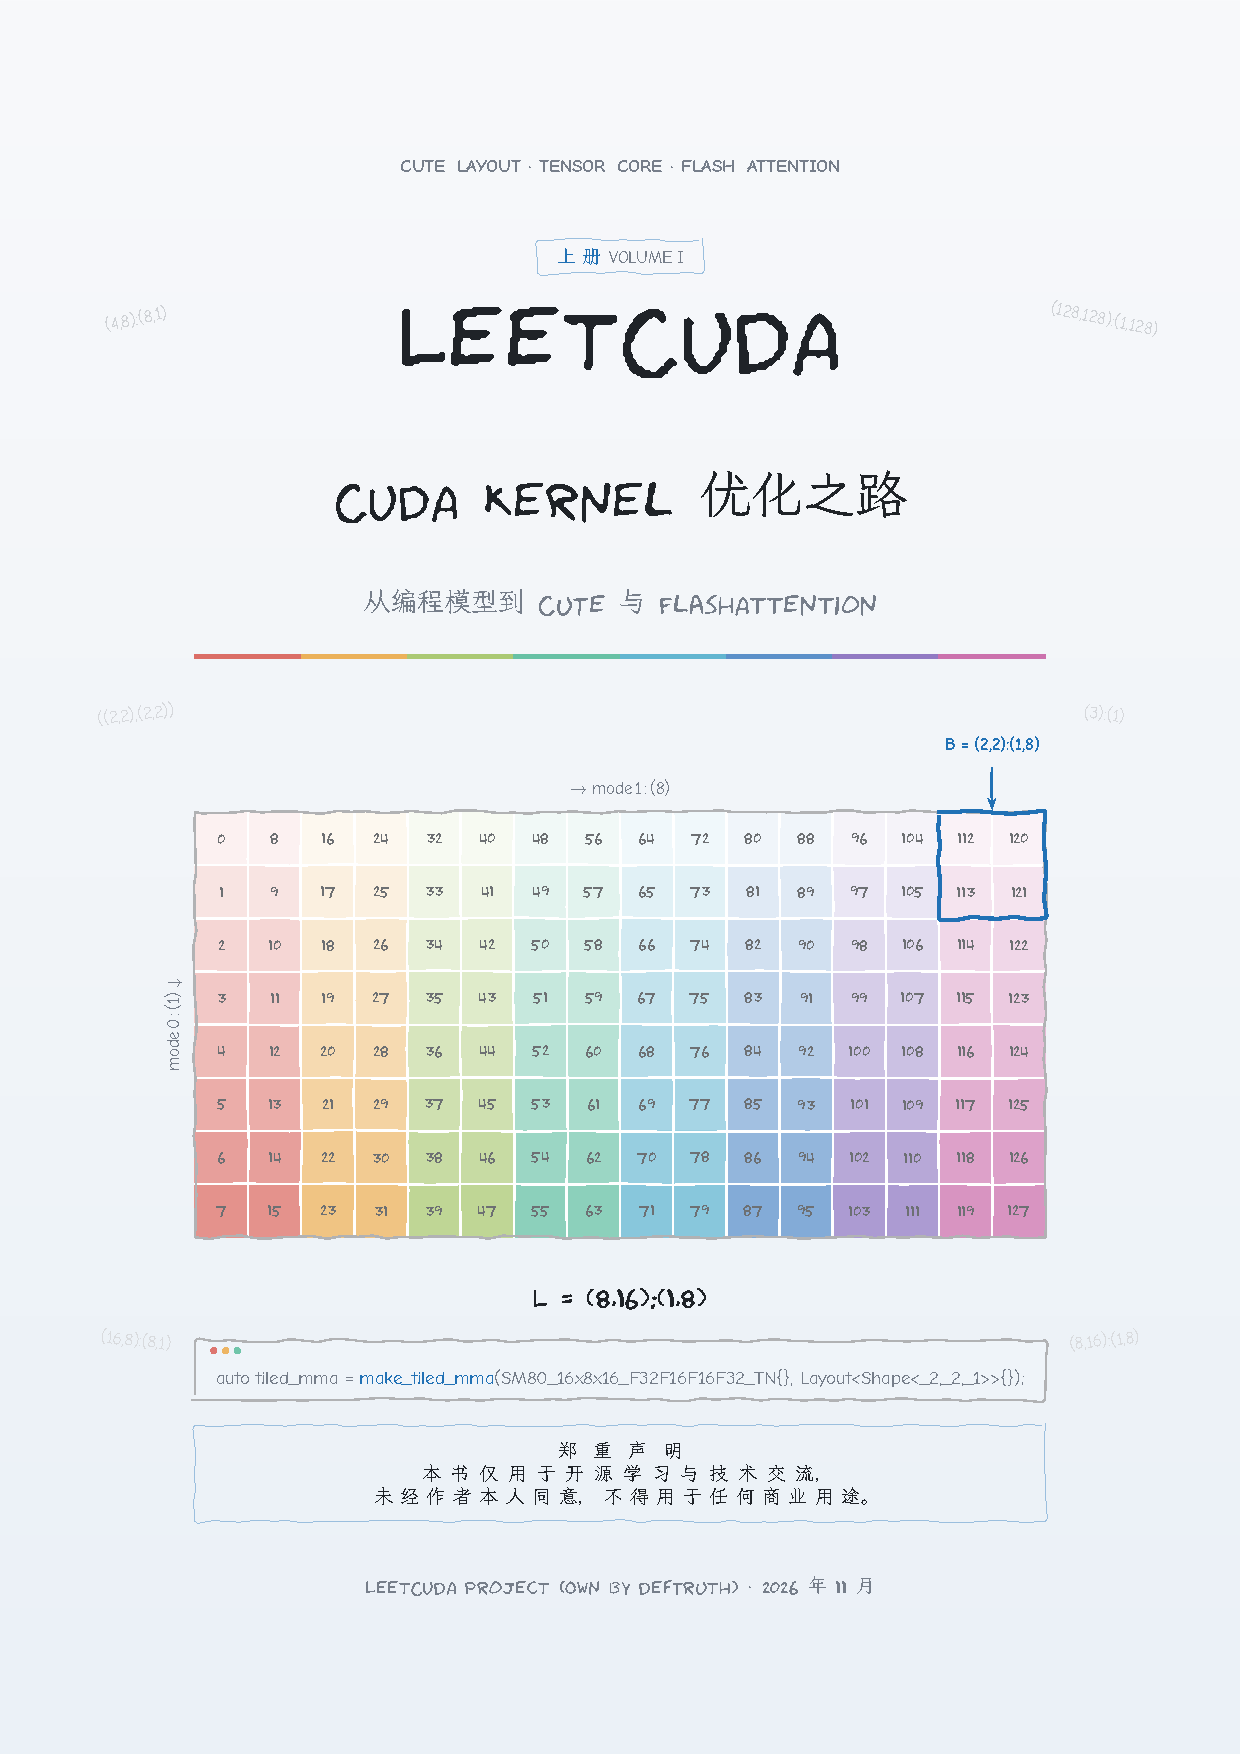
\includegraphics[width=\paperwidth,height=\paperheight]{figures/misc/cover-vol1.pdf}}}
\thispagestyle{empty}
\null
\clearpage

% 分册说明（主书不含此页）
\thispagestyle{empty}
\vspace*{0.18\textheight}
\begin{center}
  {\Large\bfseries 分册说明}\\[1.6em]
  \begin{minipage}{0.76\textwidth}
    \normalsize\linespread{1.4}\selectfont
    本书分上下两册。本册为\mbox{\textbf{上册}}，收录第一～四部分（第 1--29 章）：
    基础篇、GEMM 篇、Attention 篇与 CuTe 篇。\mbox{\textbf{下册}}收录第五～九部分
    （第 30--45 章）与附录 A--E。\par\vspace{1em}
    两册沿用全一册版的章号、图号、表号与公式编号，正文中的交叉引用可跨册对照；
    上册正文提到的附录 A、附录 B 均在下册。
  \end{minipage}
\end{center}
\clearpage

% 消除 frontmatter 的奇数开页空页，目录紧跟封面/说明
\begingroup
\let\cleardoublepage\clearpage
\frontmatter
\tableofcontents
\endgroup

% openany 电子书不强制右页起始：否则目录尾后 \mainmatter 的 \cleardoublepage 会补一页空白
\let\cleardoublepage\clearpage
\mainmatter

\part{基础篇：编程模型、访存与归约}
% ch00-profiling.tex — 性能分析先于优化：nsys 与 ncu（RFC-C0）
% 工具方法论章：无对应源码区间，无编译宏限定，全 arch 通用
% 本章无 device kernel：book/tests/ 不设 ch00 测试；实战数据引自作者参与的 CUDA kernel 开发 NCU/NSYS 分析记录
\chapter{性能分析先于优化：nsys 与 ncu}\label{ch:00}

\section{本章导读}

在动手写第一个 kernel 之前，本书先约定一条工程规则：\textbf{profile 永远都是最重要的}。
优化 GPU kernel 的正确循环不是改完跑一下看快没快，而是先测量、再假设、改一处、
再测量。凭直觉的优化，快了不知道为什么快，慢了也找不到原因。这一章讲两件测量
工具：\textbf{Nsight Systems}（nsys，全局时间线）与 \textbf{Nsight Compute}（ncu，
单 kernel 计数器），从原理、命令行用法到核心指标的含义逐一拆开，并给出一张
症状 $\to$ 证据 $\to$ 结论 $\to$ 对策的瓶颈判断决策树。

本章不含 kernel（与 ch01 及 Part IV 的原理章 ch20--22 一样，是纯理论/工具章）。
没有新代码可讲，但有大量实战教训，全部来自真实的 CUDA kernel 开发记录，涉及
寄存器压力、spill、warp stall、Tensor Core 饱和度、L1/L2 命中率、bank conflict，
每一个指标都配一个真实的指标驱动优化或指标否决优化案例。后续各章的性能分析节
都默认读者已掌握本章的工具与词汇表。

\textbf{前置}：无（与 ch01 互为入口，roofline 词汇见 ch01）。
\textbf{源码区间}：无（工具方法论章）。\textbf{编译宏与架构限定}：无。

\section{问题与动机：不 profile 就优化的代价}

三个真实的开发反例说明不 profile 就优化会错在哪里。

\textbf{反例一：感觉是装载瓶颈，其实是依赖链}。一个 sm\_89 上的 fp8
attention kernel（persist-D 结构）对标业界最快实现慢 28\%（909.4$\mu$s vs
710$\mu$s）。直觉方案是加深装载流水、减指令、缩 tile，全部实测无效；
NCU 的 stall 剖析结果直接给出结论：\texttt{math\_\allowbreak{}pipe\_\allowbreak{}throttle} 1.32
主导、\texttt{wait} 0.82、\texttt{long\_\allowbreak{}scoreboard} 仅
0.04，\textbf{装载根本不是瓶颈}：瓶颈是单 CTA 内 softmax$\to$PV 的串行
依赖链，唯一有效的改动是拆链（2 CTA/SM），实测 $-5\%$。

\textbf{反例二：感觉主 kernel 慢，其实差距在别处}。e2e 落后时先对主 kernel
跑 ncu，做完整套指标分析才发现主 kernel 已占 e2e 时间 86--92\%、前处理链
已优于对照，一次 nsys 的时间线本可以三分钟得出同样结论，避免在错误的
kernel 上浪费半天 ncu 分析。

\textbf{反例三：感觉融合更快，其实更慢}。把 softmax 的 bias 注入从分离 kernel
改成单 pass 融合 + smem tile，直觉上少一次读写应该更快，实测反而慢 4.2ms：
NCU 显示融合把 LDS（shared load）拉进了 consumer 关键路径，\texttt{sleeping}
stall 从 3.5\% 升到 22.3\%。指标否决了这次优化。

三个反例的共同教训：GPU 上的性能瓶颈很少出现在直觉指向的位置。成熟的优化
工作流会把它固化成一条硬规则：\textbf{没有 NCU 数据，不改 kernel}；每条优化结论必须
引用具体 metric 数值作为证据。

\section{工具链总览与顺序方法论}\label{sec:ch00-tools}

\subsection{两个工具回答两个不同的问题}

nsys 与 ncu 的采集原理完全不同：

\begin{itemize}
\item \textbf{nsys（Nsight Systems）}：trace 型。在驱动层记录 API
  调用、kernel launch、内存拷贝、流与事件的时间戳，拼出一张全局时间线。
  它回答时间花在哪：哪个 kernel 占比最大、kernel 之间有没有空隙（gap）、
  CPU launch 是否跟不上、多流是否真的在重叠。代价低：不需要 GPU 性能
  计数器权限，任何环境都能跑，被测程序几乎不失真。
\item \textbf{ncu（Nsight Compute）}：counter replay 型。要读一个
  kernel 的成百上千个硬件计数器（SM 吞吐、cache 命中、warp stall 等），
  而一遍执行采不完这么多计数器，于是 ncu 把 kernel 回放多遍，
  每遍采一组；为了数据可比还会锁定时钟。它回答这个 kernel 内部慢在哪。
  代价高：单 kernel 深挖、时间被串行化与放大，ncu 报告里的 kernel 耗时
  \textbf{不能当 bench 时间用}。
\end{itemize}

\subsection{顺序：先 nsys，后 ncu}

顺序不是习惯问题，是成本问题：

\begin{enumerate}
\item \textbf{nsys 先行}：一次采集拿到全部 kernel 的时间占比排序。如果主
  kernel 占 86\%，那么辅助 kernel 再慢也只有 14\% 的优化上限：先确认
  该优化谁，再谈怎么优化。nsys 还能立刻暴露三类结构性问题：launch
  gap（CPU 跟不上，一个真实案例 wall-GPU 差 129$\mu$s vs 对照 50$\mu$s，
  原因在 dispatch 而非 kernel）、该并行的流没重叠、意外的 fallback kernel。
\item \textbf{ncu 跟进}：只对 nsys 排出的 Top-1/Top-2 kernel 做
  \texttt{-{}-set full} 深挖，读 roofline、occupancy、stall、memory 各维
  指标，形成假设。
\item \textbf{单变量修改 $\to$ 复测}：每次只改一处，re-profile 后用
  \texttt{-{}-diff} 对照前后指标；无效或负优化立即回退。
\end{enumerate}

反着来的代价见反例二：先 ncu 后 nsys，等于把半天的深挖时间花在一个可能
不重要的 kernel 上。

\begin{figure}[H]
\centering
\begin{tikzpicture}[
  font=\footnotesize,
  box/.style={draw, rounded corners=2pt, align=center, inner sep=3pt,
    font=\scriptsize, text width=2.2cm, minimum height=1.0cm},
  ar/.style={-{Stealth[length=1.8mm]}, semithick}
]
  \node[box, text width=1.3cm, draw=tkRed, fill=tkFillRed, text=tkRed!80!black] (e2e) at (0.95, 0)
    {e2e\\落后};
  \node[box, draw=tkBlue, fill=tkFillBlue] (nsys) at (3.4, 0)
    {nsys 全局时间线\\\texttt{-t cuda} 单域\\kern\_sum 占比排序};
  \node[box, draw=tkBlue!70!tkPurple, fill=tkFillBlue!50!white] (top) at (6.35, 0)
    {Top-1/2 kernel\\主 kernel 占 86--92\%\\$\to$ 辅助链上限仅 14\%};
  \node[box, draw=tkBlue, fill=tkBlue!30!white] (ncu) at (9.3, 0)
    {ncu 单 kernel 深挖\\\texttt{-{}-set full}\\\texttt{regex:} 名字前缀};
  \node[box, draw=tkPurple, fill=tkFillPurple] (judge) at (12.35, 0)
    {指标判读\\（接决策树\\图~\ref{fig:0-1}）};
  \draw[ar] (e2e.east) -- (nsys.west);
  \draw[ar] (nsys.east) -- (top.west);
  \draw[ar] (top.east) -- (ncu.west);
  \draw[ar] (ncu.east) -- (judge.west);
  \node[box, draw=tkOrange, fill=tkFillOrange] (modi) at (12.35, -2.35)
    {单变量修改\\每次只改一处};
  \node[box, draw=tkOrange, fill=tkFillOrange] (diff) at (8.9, -2.35)
    {复测 \texttt{-{}-diff}\\前后指标对照};
  \node[box, draw=tkGreen, fill=tkFillGreen] (keep) at (5.2, -2.35) {有效 $\to$ 保留};
  \draw[ar] (judge.south) -- (modi.north);
  \draw[ar] (modi.west) -- (diff.east);
  \draw[ar, tkGreen] (diff.west) -- (keep.east)
    node[midway, above, font=\scriptsize, text=tkGreen] {有效};
  \node[box, draw=tkRed, dashed, fill=white, text=tkRed!80!black] (revert) at (8.9, -4.1)
    {无效 / 负优化\\$\to$ 回退};
  \draw[ar] (diff.south) -- (revert.north)
    node[midway, right, font=\scriptsize, text=tkRed] {无效};
  \draw[ar, dashed, tkRed] (revert.east) -- (14.1, -4.1) -- (14.1, 0) -- (judge.east);
  \node[font=\scriptsize, anchor=west, text=tkRed!70] at (14.25, -2.0)
    {回到判读};
\end{tikzpicture}
\caption{nsys $\to$ ncu $\to$ 单变量修改 $\to$ 复测 \texttt{-{}-diff} 的闭环工作流：nsys 先给全局占比与优化预算（主 kernel 占 86--92\%，辅助链上限仅 14\%，对应 \S\ref{sec:ch00-cases} 例一）；ncu 只深挖 Top-1/2 kernel；每次只改一处，复测后无效立即回退、回到指标判读。配色：红=问题起点，蓝=采集/分析链，紫=判读决策点，橙=修改/复测动作，绿=有效保留，红虚线=无效回退。}
\label{fig:0-2}
\end{figure}

\section{nsys 命令行实战}\label{sec:ch00-nsys}

\subsection{最小采集}

原则是只采需要的域、只采最短的窗口。对看 kernel 占比这个目标，
一条 trace 域 \texttt{-t cuda} 就够，CPU 采样与上下文切换全部关掉，warmup
与 repeat 降到最小：

\begin{lstlisting}[style=console, title={nsys 最小采集（kernel 时间占比场景）}]
nsys profile -t cuda --sample=none --cpuctxsw=none \
  -o .tmp/ch00/report.nsys-rep python bench.py
\end{lstlisting}

\subsection{stats 报表：两个最常用的 report}

采集产物是 \texttt{.nsys-rep}，用 \texttt{nsys stats} 导出统计：

\begin{lstlisting}[style=console, title={nsys stats 两个高频 report}]
nsys stats -r cuda_gpu_kern_sum report.nsys-rep   # per-kernel 时间占比（最常用）
nsys stats -r cuda_gpu_trace   report.nsys-rep   # per-launch 时间线（看 gap/流重叠）
\end{lstlisting}

\texttt{cuda\_\allowbreak{}gpu\_\allowbreak{}kern\_\allowbreak{}sum} 按 kernel 聚合总时长与占比，直接回答该优化谁
的问题；\texttt{cuda\_\allowbreak{}gpu\_\allowbreak{}trace} 逐 launch 列时间戳，用来看相邻 kernel
间的空隙与多流 overlap。首次对旧 report 运行时报
\texttt{Existing SQLite export found} 时，加 \texttt{-{}-force-export=\allowbreak{}true}
强制重新导出。

\subsection{体积控制：一次 500GB 事故}

nsys 的中间数据默认写到 \texttt{/\allowbreak{}tmp/\allowbreak{}nvidia/\allowbreak{}nsight\_\allowbreak{}systems}，体积 $\approx$
单事件字节数 $\times$ 事件数，而事件数随时长线性增长。对大模型推理（多模型链、大 seqlen、多次 repeat）不加
限制地全量采集，曾把 \texttt{/tmp} 写到 500GiB+ 直到磁盘写满系统卡死
（真实事故，2026-09）。
三条铁律：

\begin{enumerate}
\item \textbf{输出与临时文件落项目目录}：显式设 \texttt{TMPDIR} 指向项目
  \texttt{.tmp/} 下的目录并用 \texttt{-o} 指定输出，事后清理。注意 TMPDIR
  路径要短，过长的路径会超过 Unix domain socket 的 107 字节路径上限，导致
  Ray 的 plasma store 构造失败。
\item \textbf{禁止对大模型 e2e 不加限制地全量采集}：repeat 降到 0--1，单域
  \texttt{-t cuda}，关采样。
\item \textbf{优先 torch.profiler}：只想看 kernel 时间表时，
  \texttt{torch.\allowbreak{}profiler} 输出 chrome trace 落在 \texttt{.tmp/}，零外部临时
  文件风险；nsys 只在必须看时间线/同步事件时使用。
\end{enumerate}

\subsection{窗口化采集：cudaProfilerApi}

只想采推理中的一小段（比如 50 个 denoise step 中的 1 步）时，用
\texttt{-{}-capture-range=\allowbreak{}cuda\allowbreak{}Profiler\allowbreak{}Api} 配合代码里的开关，把采集窗口限定在
目标区间：

\begin{lstlisting}[style=console, title={窗口化采集（Python 侧）}]
nsys profile -t cuda --capture-range=cudaProfilerApi \
  --sample=none --cpuctxsw=none -o .tmp/ch00/win python bench.py
# bench.py 内：
#   torch.cuda.profiler.start()   # 窗口开始
#   ... 目标 step ...
#   torch.cuda.profiler.stop()    # 窗口结束
\end{lstlisting}

\section{ncu 命令行实战}\label{sec:ch00-ncu}

\subsection{基础采集与 section}

\begin{lstlisting}[style=console, title={ncu 全量采集与 CSV 导出}]
ncu --set full -o .tmp/ch00/report_v1 --target-processes all ./kernel_app
ncu --import .tmp/ch00/report_v1.ncu-rep --page raw --csv > report_v1.csv
\end{lstlisting}

\texttt{-{}-set full} 采全部 section（roofline、occupancy、warp state、
memory workload、instruction mix 等），单 kernel 回放多遍、耗时可观；快速
确认可用默认 basic set。交互式 \texttt{ncu-ui} 看报告，命令行用
\texttt{-{}-page details}（rule-based 汇总）或 \texttt{-{}-page raw}（原始
metric，见下）。

\subsection{-{}-kernel-name 必须用 regex: 前缀}

C++ 模板 kernel 的完整名带一长串后缀（如
\texttt{persist\_\allowbreak{}d\_\allowbreak{}ws\_\allowbreak{}fwd\_\allowbreak{}cute\_\allowbreak{}fp8\_\allowbreak{}sm120}，实际实例化名比这更长）。
\texttt{-{}-kernel-name} 默认精确匹配，拿名字前缀去匹配会报
\texttt{No kernels were profiled} 且生成空 report。必须加 \texttt{regex:}
前缀走部分匹配：

\begin{lstlisting}[style=console, title={kernel 名过滤：regex 前缀}]
ncu --set full -o rep --kernel-name regex:persist_d_ws_fwd_cute_fp8 \
  --target-processes all ./app     # OK：部分匹配
ncu --kernel-name persist_d_ws_fwd_cute_fp8_sm120 ...  # 错：精确匹配，0 命中
\end{lstlisting}

\subsection{-{}-page raw 提取原始 metric}

ncu 的 \texttt{-{}-csv} 默认输出是 rule-based 的 section 汇总（按
诊断规则组织），不是逐个原始计数器。要拿具体 stall reason 的数值，必须走
\texttt{-{}-page raw}。raw 输出里每个 metric 占三行：名字、单位、数值，
用 \texttt{grep -A3} 抓：

\begin{lstlisting}[style=console, title={从 raw page 提取 stall 指标}]
ncu --import rep.ncu-rep --page raw 2>&1 | \
  grep -A3 "warps_issue_stalled_\(wait\|math_pipe_throttle\|sleeping\)"
\end{lstlisting}

\subsection{权限限制与同架构代理 GPU}

读性能计数器需要驱动授权。容器/云主机上常见
\texttt{/proc/\allowbreak{}driver/\allowbreak{}nvidia/\allowbreak{}params} 里
\texttt{Rm\allowbreak{}Profiling\allowbreak{}Admin\allowbreak{}Only} 标志为 1，
此时 \texttt{-{}-set full} 直接报 \texttt{ERR\_\allowbreak{}NVGPUCTRPERM}，且容器内无法
reload 驱动。可行解法是同架构代理：找一块相同微架构的本地 GPU 跑
ncu，例如用本地 RTX PRO 5000（sm\_120a）代理远端 RTX 5090（sm\_120）。
stall reasons、指令 mix、occupancy 这类架构级结论可以迁移，绝对
性能数字（SM 数、频率、L2 容量）不可迁移；ncu 验证完架构结论后，回目标
硬件跑 timing bench 收数。

\subsection{replay 的干扰与 A/B 规则}

ncu 锁频 + 多遍回放 + 串行执行，因此报告内耗时只用于相对比较。做优化 A/B
时回到真实 bench，并遵守两条规则：

\begin{itemize}
\item \textbf{校验公共参照}：许多 bench 会同时输出被测实现与公共参照
  （如 PyTorch SDPA）两组时间；对比前先核对两轮参照是否吻合（$\pm$1\%）。
  被 GPU 级干扰（并发进程/时钟态）污染的一轮，两者会同比例膨胀
  （实测约 $2\times$），直接对比会得出 $-50\%$ 全面加速这种物理上不可能
  的假结论。
\item \textbf{min-of-N 口径}：单轮抖动大的实现（如 tma 变体）取 N 次最小值
  对比；归因 race 类问题必须 stash $\to$ 重建 $\to$ 同 probe 的 HEAD 对照，
  单次好结果不可信。
\end{itemize}

\section{核心指标字典}\label{sec:ch00-metrics}

以下每个指标按含义、怎么读、异常意味着什么、对策逐项展开。数值口径以
sm\_120 上的实测为参照。

\subsection{SpeedOfLight：SM\% 与 MEM\%（roofline 定位）}

\texttt{sm\_\allowbreak{}\_\allowbreak{}throughput}（SM\%）与 \texttt{gpu\_\allowbreak{}\_\allowbreak{}compute\_\allowbreak{}memory\_\allowbreak{}throughput}
（MEM\%）分别是计算管线与内存管线的峰值利用率，是 NCU 报告的第一行。
两者把 kernel 放上 ch01 的 roofline：SM\% 高 MEM\% 低是 compute-bound，
反之 memory-bound；\textbf{双低}（如 SM/MEM 都在 30\% 附近）则是
latency-bound：两条管线都没有饱和，问题在并行度或依赖链，这是 roofline 图上
看不出的第三态，必须回到 stall 指标找证据。

\subsection{Occupancy：理论、达到与三类限制源}

区分两个数：\textbf{理论 occupancy}（kernel 资源能驻留多少 warp，受寄存器、
smem、block/warp 上限三类限制源钳制）与\textbf{达到 occupancy}
（\texttt{sm\_\allowbreak{}\_\allowbreak{}warps\_\allowbreak{}active}，实际运行均值，受 tail effect 与负载不均
拖累）。NCU 的 Occupancy section 会明确指出 \texttt{launch\_\allowbreak{}\_\allowbreak{}occupancy\_\allowbreak{}limit\_\allowbreak{}registers} /
\texttt{\_\allowbreak{}\_\allowbreak{}shared\_\allowbreak{}mem} / \texttt{\_\_blocks} 哪个是当前限制源。一个
fp8 attention kernel 的实例：WS 结构（4 producer + 8 consumer，共 384 线程）的
launch 配置按 $65536/384$ 把静态寄存器压到 168，\texttt{Block Limit Registers} 因此恒为 1；
稳态再按 \texttt{setmaxnreg} 分成 $128\times32 + 256\times232 = 63{,}488$ 个，占满寄存器池，
第二个 CTA 需要 126{,}976，故 1 CTA/SM、12 warps，理论 occupancy
25\%（12/48），此时想提并行度只有降寄存器或换结构
（见 \S\ref{sec:ch00-cases} 例二）。注意 ch01 的告诫：occupancy 是手段不是
KPI，GEMM 类 kernel 用大 tile + 低 occupancy + 高 ILP 换性能是常态。

\begin{figure}[H]
\centering
\begin{tikzpicture}[font=\footnotesize,
  lab/.style={font=\scriptsize, inner sep=1pt}]
  \draw[-{Stealth[length=1.8mm]}] (0, 0) -- (13.3, 0);
  \draw[-{Stealth[length=1.8mm]}] (0, 0) -- (0, 6.75);
  \foreach \x/\t in {1.44/32, 2.88/64, 5.76/128, 8.64/192, 11.52/256}
    {
      \draw (\x, 0) -- (\x, -0.08);
      \node[lab, anchor=north] at (\x, -0.1) {\t};
    }
  \foreach \y/\t in {0.92/8, 1.84/16, 2.76/24, 3.68/32, 4.60/40}
    {
      \draw (0, \y) -- (-0.08, \y);
      \node[lab, anchor=east] at (-0.1, \y) {\t};
    }
  \draw (0, 5.52) -- (-0.08, 5.52);
  \node[lab, anchor=east, font=\scriptsize\bfseries] at (-0.1, 5.52) {48};
  \draw[tkBlue, semithick] plot[smooth] coordinates
    {(1.44,5.52) (1.92,5.52) (2.16,4.91) (2.52,4.21) (2.88,3.68) (3.24,3.27) (3.60,2.94)
     (4.32,2.45) (5.04,2.10) (5.76,1.84) (7.20,1.47) (8.64,1.23) (10.08,1.05)
     (11.52,0.92)};
  \draw[tkOrange, semithick] (0.3, 2.76) -- (7.9, 2.76);
  \draw[tkPurple, semithick] (0.3, 5.52) -- (11.8, 5.52);
  \draw[very thick]
    (0.3,2.76) -- (3.83,2.76) -- (3.83,1.84)
    -- (5.76,1.84) -- (5.76,0.92) -- (11.52,0.92);
  \node[lab, anchor=south west, text=tkPurple] at (4.7, 5.72) {block/warp 槽位上限：48 warps};
  \node[lab, anchor=north west, align=left, text=tkOrange] at (0.4, 2.56)
    {smem 约束（示例：\\smem/block=32KB，T=256）\\$\to$ 3 blocks = 24 warps};
  \node[lab, anchor=west, align=left, text=tkBlue] at (11.68, 0.92)
    {寄存器约束\\$65536/(32r)$};
  \node[lab, anchor=west, align=left] at (11.68, 2.35)
    {粗黑阶梯 = min\\（整 block 量化，\\T=256 $\to$ 8 warps/级）};
  \fill (11.48, 1.38) circle (0.07);
  \draw[black!60, thin] (9.8, 4.1) -- (11.42, 1.47);
  \node[lab, anchor=north west, align=left] at (8.45, 5.25)
    {实测点（WS 结构，例二）：\\consumer REG 232 / producer 32\\
     1 CTA/SM = 12 warps（384T）\\理论 occupancy 25\%（12/48）};
  \node[lab, anchor=north] at (6.65, -0.42) {每线程寄存器数 $r$（regs/thread）};
  \node[lab, rotate=90, anchor=south] at (-0.95, 3.3) {可驻留 warp/SM};
\end{tikzpicture}
\caption{理论 occupancy 的三限制源取 min（sm\_120，48 warp 槽位口径）：寄存器约束 $65536/(32r)$（warp 粒度简化）随每线程寄存器数 $r$ 下降；smem 与槽位为水平约束（示例：smem/block=32KB、T=256，sm\_120 的 100KB/SM $\to$ 3 blocks $=$ 24 warps）。粗黑阶梯为按整 block（T=256，8 warps/block）量化的 min 包络；实测点为 WS 结构（producer 32 / consumer 232 regs）1 CTA/SM = 12 warps（384T），理论 occupancy 25\%（12/48）。}
\label{fig:0-3}
\end{figure}

\subsection{寄存器与 spill：255 墙}

\texttt{launch\_\allowbreak{}\_\allowbreak{}registers\_\allowbreak{}per\_\allowbreak{}thread} 给出每线程寄存器数，硬上限
255（每线程）。超限时编译器把变量溢出到 local memory（SASS 里表现为
\texttt{LDL}/\texttt{STL} 指令，NCU 里看
\texttt{l1tex\_\allowbreak{}\_\allowbreak{}t\_\allowbreak{}bytes\_\allowbreak{}pipe\_\allowbreak{}lsu\_\allowbreak{}mem\_\allowbreak{}\allowbreak{}local\_\allowbreak{}op\_\allowbreak{}\_\allowbreak{}ld/\allowbreak{}st.sum} 是否非零）。
编译期排查用 \texttt{-{}-ptxas-options=\allowbreak{}-v} 与
\texttt{cuobjdump -{}-dump-resource-usage} 的 STACK 字节。两个实战要点：

\begin{itemize}
\item spill 的代价主要不是流量。一个 fp4 attention kernel 在 D=512 时
  spill 总量 234MB，但 local 流量仅 12.8GB/s，带宽不是瓶颈；真正的代价是
  \textbf{延迟暴露}：8 warps/SM 意味着每 scheduler 只有 2 个 warp 可切换，
  LDL 的几百 cycle 延迟藏不住，同时指令数也变多。
\item 寄存器预算可以算出来。attention 的 O 累加器每线程占
  $k_{Br}\cdot D/256$ 个 f32 寄存器（M8N1 布局，$256=32$ lanes $\times 8$
  个 warp，对应 consumer 全部 256 线程）；$k_{Br}{=}128$ 时为
  $D/2$，D=512 要 256 个，超出 255 寄存器上限。大 D 必须换
  M4N2 atom（列拆给两个 warp，每线程 $D/4$）的数学来源就在这里（ch19）。
\end{itemize}

\subsection{Warp State：stall reasons，好 stall 与坏 stall}

warp 每个周期若不能发射，必有一个停滞原因。sm\_120 上的口径是
\texttt{smsp\_\allowbreak{}average\_\allowbreak{}warps\_\allowbreak{}issue\_\allowbreak{}stalled\_\allowbreak{}*\_\allowbreak{}per\_\allowbreak{}issue\_\allowbreak{}active.\allowbreak{}ratio}
，即每个发射周期停在该原因上的平均 warp 数。表~\ref{tab:00-stall}
是实战中最常读的八项：

\begin{table}[htbp]
\centering
\caption{warp stall 指标字典（sm\_120 实测口径）}
\label{tab:00-stall}
\begin{tabular}{lp{5.2cm}p{5.6cm}}
\toprule
指标后缀 & 含义 & 高值时怎么办 \\
\midrule
\texttt{wait} & 固定延迟依赖（寄存器/ALU 结果未就绪） & 依赖链问题：拆链、增并行 warp、重排指令；attention 的 softmax$\to$PV 串行链是典型来源 \\
\texttt{long\_\allowbreak{}scoreboard} & 等 gmem/TMA 数据 & 装载不足：\texttt{cp.async}/TMA、加深 stage、prefetch \\
\texttt{short\_\allowbreak{}scoreboard} & 等 smem（MIO 队列） & LDS 链太长：swizzle 布局、减少 smem 往返 \\
\texttt{math\_\allowbreak{}pipe\_\allowbreak{}throttle} & 数学管线排队满 & \textbf{好信号}：计算饱和。保持或进一步减 FLOPs \\
\texttt{sleeping} & warp 休眠（mbarrier 退避） & \textbf{纯浪费}：producer/consumer 失衡或空转自旋，查 WS 结构 \\
\texttt{barrier} & 等显式栅栏 & 同步过频：减少 \texttt{\_\allowbreak{}\_\allowbreak{}syncthreads} 点、缩 block \\
\texttt{not\_\allowbreak{}selected} & 就绪但调度器选中了其他 warp & \textbf{健康}：有冗余并行度可隐藏延迟 \\
\texttt{selected} & 正在发射（非停滞） & 基线，越大越好 \\
\bottomrule
\end{tabular}
\end{table}

读 stall 剖析结果的关键是分好坏：\texttt{math\_\allowbreak{}pipe\_\allowbreak{}throttle} 与
\texttt{not\_\allowbreak{}selected} 高说明计算与调度资源在正常工作（但
\texttt{math\_\allowbreak{}pipe\_\allowbreak{}throttle} 高还须与 \texttt{pipe\_\allowbreak{}tensor} 交叉验证：
例三中 mpt $=1.32$ 而 tensor pipe 仅 $49\%$，并非 Tensor Core 饱和）；\texttt{sleeping} 高几乎总是结构
问题；\texttt{wait} 与 \texttt{long\_\allowbreak{}scoreboard} 的相对大小直接
区分依赖链受限与装载受限，例见 \S\ref{sec:ch00-cases} 例三。

\subsection{Memory Workload：L1/L2/DRAM 分层归因}

三层各看命中率与吞吐两个数：

\begin{itemize}
\item \textbf{L1/TEX}：\texttt{l1tex\_\allowbreak{}\_\allowbreak{}t\_\allowbreak{}sector\_\allowbreak{}hit\_\allowbreak{}rate.pct}。低于
  20\% 且数据本该复用时，考虑 tiling 进 smem 或改访问模式。注意 smem 与 L1
  共池（GB202 实测每多占 16KB smem，kernel 约慢 4--5$\mu$s），
  多分 smem 不是免费的。
\item \textbf{L2}：\texttt{lts\_\allowbreak{}\_\allowbreak{}t\_\allowbreak{}sector\_\allowbreak{}hit\_\allowbreak{}rate.\allowbreak{}pct}。大 GEMM 上低
  命中可用 CTA swizzle / StreamK 提数据局部性；推理场景 K/V 重复读高命中
  是常态。
\item \textbf{DRAM}：\texttt{dram\_\allowbreak{}\_\allowbreak{}throughput}（峰值百分比）。接近饱和
  （$>$70\%）说明带宽墙已到，优化方向只剩减流量（混合精度、融合、去
  物化）。一条量化前处理链实测达到饱和带宽 1.04TB/s（约为理论峰值
  1344GB/s 的 77\%）。此时融合省 launch 已无杠杆，只有减流量才有收益。
\item \textbf{load/store 与合并访问}：global load 的每请求扇区数
  （\texttt{l1tex} 前缀的
  \texttt{average\_\allowbreak{}t\_\allowbreak{}sectors\_\allowbreak{}\_\allowbreak{}per\_\allowbreak{}request\_\allowbreak{}\allowbreak{}...} 系列指标）
  衡量合并访问质量：32-bit 连续访问的理想值是 4（一个 warp 的 128B 恰好
  4 个 32B sector）。明显超标说明访存发散，流量被放大，对策是内维连续、
  向量化（\texttt{float4} 128-bit 访存，ch03）与 AoS$\to$SoA。IO 压力要从
  三个正交维度一起看：吞吐（哪层饱和）、命中率（数据该由哪层负责）、
  合并度（流量有没有被访问模式放大）。
\end{itemize}

分层归因顺序：DRAM 饱和先看是不是 L2 miss 推的（L2 hit 低 + DRAM 高 =
工作集溢出），L2 高命中但 L1 低命中 = smem/L1 复用不足。IO 压力的层
定位错了，对策就全错。

\subsection{bank conflict 与 smem 指标}

\texttt{l1tex\_\allowbreak{}\_\allowbreak{}data\_\allowbreak{}bank\_\allowbreak{}conflicts\_\allowbreak{}pipe\_\allowbreak{}lsu\_\allowbreak{}mem\_\allowbreak{}\_\allowbreak{}shared\_\allowbreak{}op\_\allowbreak{}ld/\allowbreak{}st.sum}
直接数冲突次数（ch12 表 12-1 的数据来源）。判读要点是先看占比再动手：
曾有一个消除 O 写回 bank conflict 的优化立项，NCU 一查 ld conflict 仅 0.39\%，
且 MUFU 等待被 MMA 掩盖，整个方向当场否决。冲突计数要换算成每 warp 每 cycle
的额外重放次数才能反映实际影响，绝对数大不等于值得修。

\subsection{指令 mix 与 tensor pipe 利用率}

各执行管线的活跃占比（\texttt{pipe\_fma} / \texttt{pipe\_alu} /
\texttt{pipe\_lsu} / \texttt{pipe\_tensor}）回答指令都花在哪。
对本书 Part II--IV 的主线而言，tensor pipe 利用率就是 Tensor Core 饱和度：
fp16 GEMM 类 kernel 若 \texttt{pipe\_fma} 高而 \texttt{pipe\_tensor}
低，说明还在用 CUDA Core 算乘加，应该换 MMA 指令（ch10--11 的主题）。
一个 fp8 kernel 的实例：tensor pipe 从 49\% 提到 59.5\% 的那次优化，
判据是 \texttt{math\_\allowbreak{}pipe\_\allowbreak{}throttle} 降了、tensor pipe 升了，两条
指标共同确认依赖链被拆开、Tensor Core 利用率提高。

\section{瓶颈判断决策树}\label{sec:ch00-tree}

把上述指标串成一条判断流程（数值阈值为工程经验值，非硬边界）：

\begin{figure}[H]
\centering
\begin{tikzpicture}[
  font=\footnotesize,
  box/.style={draw, rounded corners=2pt, align=center, inner sep=3pt,
    text width=2.6cm, minimum height=8mm},
  dec/.style={box, draw=tkBlue, fill=tkFillBlue},
  memb/.style={box, draw=tkOrange, fill=tkFillOrange},
  cpub/.style={box, draw=tkPurple, fill=tkFillPurple},
  latb/.style={box, draw=tkRed, fill=tkFillRed},
  balb/.style={box, draw=tkGreen, fill=tkFillGreen},
  det/.style={draw, align=left, inner sep=3pt, font=\scriptsize,
    text width=5.1cm, fill=white},
  detm/.style={det, draw=tkOrange!85},
  detc/.style={det, draw=tkPurple!85},
  detl/.style={det, draw=tkRed!85},
  badge/.style={circle, draw=tkBlue!80!black, fill=tkBlue!30, inner sep=0pt,
    minimum size=3.6mm, font=\scriptsize\bfseries, anchor=south east},
  ar/.style={-{Stealth[length=1.8mm]}, semithick},
  arm/.style={ar, draw=tkOrange},
  arc/.style={ar, draw=tkPurple},
  arl/.style={ar, draw=tkRed!85}
]
  \node[dec] (root) at (0, 0.55) {读 SOL\\（SM\% / MEM\%）};
  \node[badge] at (root.north west) {1};
  \node[memb] (mcond) at (3.8, 4.2) {MEM\% $\gg$ SM\%\\（差 $>$20）};
  \node[memb] (mver) at (7.9, 4.2) {memory-bound\\分层归因};
  \node[badge] at (mver.north west) {4};
  \node[detm] (md1) at (12.9, 5.4) {DRAM $>$70\% $\to$ 带宽墙\\对策：减流量（融合 / 低精度 / 去物化）};
  \node[detm] (md2) at (12.9, 4.2) {L2 hit $<$50\% 且 DRAM $>$40\%\\$\to$ 工作集 / L2 局部性（CTA swizzle）};
  \node[detm] (md3) at (12.9, 3.0) {L1 hit $<$20\% 而 L2 高\\$\to$ smem tiling / 复用不足};
  \node[cpub] (ccond) at (3.8, 1.2) {SM\% $\gg$ MEM\%};
  \node[cpub] (cver) at (7.9, 1.2) {compute-bound\\查饱和质量};
  \node[badge] at (cver.north west) {5};
  \node[detc] (cd1) at (12.9, 1.8) {tensor pipe 高 = 健康\\$\to$ 减 FLOPs 或更低精度};
  \node[detc] (cd2) at (12.9, 0.6) {pipe\_fma / alu 高、tensor 低\\$\to$ 该上 MMA 指令（ch10--11）};
  \node[latb] (lcond) at (3.8, -1.8) {双低\\（都 $<$40）};
  \node[latb] (lver) at (7.9, -1.8) {latency-bound\\stall 前二名分流};
  \node[badge] at (lver.north west) {2};
  \node[detl] (ld1) at (12.9, -0.6) {\texttt{wait} / \texttt{math\_pipe\_throttle} 主导\\$\to$ 拆链、增并行 warp};
  \node[detl] (ld2) at (12.9, -1.8) {\texttt{long\_scoreboard} 主导\\$\to$ 异步装载（TMA / cp.async）};
  \node[detl] (ld3) at (12.9, -3.0) {\texttt{sleeping} / \texttt{barrier} 主导\\$\to$ 重排 producer/consumer（WS）};
  \node[detl, dashed, text width=5.5cm] (occ) at (7.9, -4.55) {先查 occupancy 限制源：\\limiter = regs/smem $\to$ 先解资源\\（缩 tile、降 stage、launch\_bounds）\\\textbf{增并行 warp}以有 warp 可增为前提};
  \node[badge] at (occ.north west) {3};
  \node[balb] (dcond) at (3.8, -6.15) {双高\\（都 $>$60）};
  \node[balb] (dver) at (7.9, -6.15) {接近平衡上限\\$\to$ 停止优化};
  \draw[ar, draw=tkBlue] (root.east) -- (mcond.west);
  \draw[ar, draw=tkBlue] (root.east) -- (ccond.west);
  \draw[ar, draw=tkBlue] (root.east) -- (lcond.west);
  \draw[ar, draw=tkBlue] (root.east) -- (dcond.west);
  \draw[arm] (mcond) -- (mver);
  \draw[arc] (ccond) -- (cver);
  \draw[arl] (lcond) -- (lver);
  \draw[ar, draw=tkGreen] (dcond) -- (dver);
  \draw[arm] (mver.east) -- (md1.west);
  \draw[arm] (mver.east) -- (md2.west);
  \draw[arm] (mver.east) -- (md3.west);
  \draw[arc] (cver.east) -- (cd1.west);
  \draw[arc] (cver.east) -- (cd2.west);
  \draw[arl] (lver.east) -- (ld1.west);
  \draw[arl] (lver.east) -- (ld2.west);
  \draw[arl] (lver.east) -- (ld3.west);
  \draw[arl, dashed] (lver.south) -- (occ.north);
\end{tikzpicture}
\caption{瓶颈判断决策树：先读 SOL（SM\%/MEM\%）四分流——蓝为入口判断，橙为 memory-bound 链，紫为 compute-bound 链，红为 latency-bound 链，绿为双高（停止优化）；对策框白底、边框沿用所属分支色。节点角标 1--5 对应正文 enumerate 步骤（阈值为工程经验值）。}
\label{fig:0-1}
\end{figure}

\begin{enumerate}
\item \textbf{先看 SOL}：MEM\% $\gg$ SM\%（差 $>$20）$\to$ memory-bound，
  进第 4 步；SM\% $\gg$ MEM\% $\to$ compute-bound，进第 5 步。双低
  （都 $<$40）$\to$ latency/依赖链问题，进第 2 步；双高（都 $>$60）$\to$
  已接近平衡上限，停止优化。
\item \textbf{latency-bound 分流}（看 stall 前二名）：\texttt{wait} 或
  \texttt{math\_\allowbreak{}pipe\_\allowbreak{}throttle} 主导 $\to$ 依赖链/发射受限，对策是拆链
  （拆 CTA、拆 warp 分工）或增并行 warp。\texttt{long\_\allowbreak{}scoreboard} 主导
  $\to$ 数据供给不足，对策是异步装载（\texttt{cp.async}/TMA）与加深流水。
  \texttt{sleeping}/\texttt{barrier} 主导 $\to$ 同步结构问题，对策是重排
  producer/consumer 与栅栏。
\item \textbf{查 occupancy 是否是限制源}：若 achieved 低且 limiter 是
  registers/smem，先解决资源（缩 tile、降 stage、\texttt{\_\allowbreak{}\_\allowbreak{}launch\_\allowbreak{}bounds\_\allowbreak{}}），
  因为第 2 步的增并行 warp 以有 warp 可增为前提。
\item \textbf{memory-bound 分层}：DRAM $>$70\% $\to$ 带宽墙，减流量；
  L2 hit $<$50\% 且 DRAM $>$40\% $\to$ 工作集/L2 局部性问题；L1 hit $<$20\%
  而 L2 高 $\to$ smem tiling/复用不足。顺带查 coalescing 与 bank conflict。
\item \textbf{compute-bound 查饱和质量}：tensor pipe 高 = 健康，优化转向
  减 FLOPs 或换更低精度；tensor pipe 低而 fma/alu 高 = 该上 MMA；指令数
  本身异常大时查发散与编译器胶水指令。
\end{enumerate}

\begin{table}[htbp]
\centering
\caption{症状 $\to$ 证据 $\to$ 结论 $\to$ 对策速查}
\label{tab:00-tree}
\begin{tabular}{p{3.4cm}p{4.2cm}p{2.6cm}p{4.4cm}}
\toprule
症状 & 指标证据 & 结论 & 对策 \\
\midrule
e2e 慢但不知谁慢 & nsys kern\_sum 占比 & 定位目标 kernel & 只对 Top-1/2 跑 ncu \\
kernel 慢、带宽未饱和 & MEM\%$\le$40，wait/mpt 主导 & 依赖链受限 & 拆链、2 CTA/SM、增并行 warp \\
装载等数据 & long\_scoreboard 高 & 供给不足 & TMA/cp.async、加深 stage \\
并行度上不去 & occupancy 低 + limiter=regs & 寄存器上限 & 缩 tile、M4N2 拆列、launch\_bounds \\
local ld/st 非零 & LDL/STL、local bytes & spill & 降每线程状态、查 255 寄存器上限 \\
空转严重 & sleeping 高 & WS 失衡 & 重排 producer/consumer \\
带宽饱和 & DRAM $>$70\% & 带宽墙 & 减流量：融合/低精度/去物化 \\
smem 访问慢 & bank conflicts 高 & 冲突重放 & swizzle/pad（ch12） \\
TC 没用上 & pipe\_tensor 低 & CUDA Core 算矩阵 & 换 mma/wgmma 指令 \\
\bottomrule
\end{tabular}
\end{table}

\section{实战三例：占比、寄存器与 stall}\label{sec:ch00-cases}

\subsection{例一：nsys 先行——占比决定优化预算}

场景：一个 fp8/fp4 量化 attention 库的 e2e（含量化前处理链）对标业界实现。
e2e 一度落后，最初的直觉是辅助链 kernel 太多（每 call 约 13 个），应该融合成
一个 Mega Kernel。先用全局视角（nsys + 每 kernel 带宽核算）确认：大 N 场景
主 kernel 占 e2e 时间 86--92\%，而 aux 链每个 kernel 都已达到实测饱和带宽
1.04TB/s：融合只能省 launch 不能减流量，大 N wall 差实测 $<$0.2\%，方向证伪；
真正的杠杆在主 kernel 与引擎层 overlap。方法论上，占比数据先给出优化预算上限
（占 e2e 14\% 的部分提不出 30\% 的收益），带宽核算再判这部分还有没有优化空间。

\subsection{例二：寄存器压力——255 墙、spill 与 setmaxnreg 的取舍}

场景：fp8 persist-D kernel 采用 warp specialization（WS）：1 个 producer
warp group（128T，专职 TMA）+ 1 个 consumer（256T，全计算），用
\texttt{setmaxnreg} 把寄存器从 producer（32 个）再分配给 consumer（232 个）。
寄存器压力的证据链分三层：

\begin{itemize}
\item \textbf{静态}：\texttt{cuobjdump -{}-dump-resource-usage}（D=768，
  sm\_120f）：fp8 split\_d REG:255 + STACK 1104--1944B（重 spill）；fp8
  m4n2 REG:255 + STACK 0--264B（几乎无 spill）；fp16 split\_d REG:196--254
  + STACK 约 1536B。STACK 字节就是溢出到 local 的体积。（REG:255 是非 WS 的
  128T 变体静态值；本章例二的 384T WS 变体 launch 分配是 168，见下条。）
\item \textbf{动态}：NCU 确认 \texttt{Block Limit Registers=1}——384 线程的静态上限
  168（$65536/384$ 按 8 寄存器/线程的分配粒度向下取整）只够 1 个 CTA，稳态 WS 配额 $128\times32 + 256\times232 = 63{,}488$ 又占满寄存器池
  （第二个 CTA 需 126{,}976）；理论 occupancy 25\%（12 warps/48），smem 守卫恒空转，
  限制源唯一。
\item \textbf{取舍}：consumer 需要更多寄存器（\texttt{setmaxnreg} 上限
  232，实测 224--232 区间性能平坦），但 O 累加器 $D/2$（M8N1）在 D=512 时
  要 256 个，超出 255 寄存器上限，于是 split-D 的 WS 变体被整体禁用，大 D 改走
  M4N2 把每线程压力降到 $D/4$。这是寄存器文件利用率、occupancy 与算法结构
  三方权衡的标准案例：把寄存器降下来不一定有利，要看选出的工作点能否让 tile、
  并行度与 spill 同时可接受。
\end{itemize}

（注意 \texttt{setmaxnreg} 是否被丢弃与 arch 后缀无关：\texttt{sm\_120a} 与
\texttt{sm\_120f} 都完整支持并保留该指令。真正决定它的是 TMA 的目的地址
空间：写成 \texttt{shared::cluster} 会被 ptxas 以 C7506 静默丢弃，写成
\texttt{shared::cta} 则保留。此外还有
\texttt{\_\allowbreak{}\_\allowbreak{}launch\_\allowbreak{}bounds\_\allowbreak{}} 的第二参数
（缺则 C7508 丢弃）。见第~\ref{ch:14}~章坑二。）

\subsection{例三：stall 证据链——好 stall 与坏 stall 的判读}

场景：sm\_89 fp8 persist-D 909.4$\mu$s vs 业界实现 710$\mu$s
（慢 28\%）。NCU 剖析结果：

\begin{itemize}
\item \texttt{math\_\allowbreak{}pipe\_\allowbreak{}throttle} 1.32（第一名）、
  \texttt{wait} 0.82、\texttt{long\_\allowbreak{}scoreboard} 0.04、tensor
  pipe 49\%、255 regs、1 CTA/SM。
\item 判读：\texttt{long\_\allowbreak{}scoreboard} 近零 $\Rightarrow$ 装载不是瓶颈，
  一切加深流水、减指令、缩 tile 的尝试全部无效（后续 6 项实验全部证伪，
  原因就是没先读这组数）；\texttt{mpt} 高但 tensor pipe 只有 49\% $\Rightarrow$
  管线在排队却没排满 Tensor Core，说明依赖链/发射受限。
\item 对策与验证：kBr=64 + kBc=64 + 128T（2 CTA/SM 拆链）$\to$ 864$\mu$s
  （$-5\%$），ncu 确认 2 blocks/SM、每线程寄存器降到 250；
  指标闭环：mpt 1.32$\to$0.72、tensor pipe 49\%$\to$59.5\%，
  排队变短、TC 利用率更高，与 wall 时间下降互为印证。
\end{itemize}

同族的坏 stall 案例：bias 注入的 smem tile 版本 \texttt{sleeping} 从
3.5\% 涨到 22.3\%（SASS 采样里 \texttt{SYNCS.\allowbreak{}PHASECHK} mbarrier 自旋占
18\%）：LDS 进了 consumer 关键路径、两级 QK 流水供不上，全 warp 自旋等 K，
该版本被指标否决。

\section{常见坑}

\begin{enumerate}
\item \textbf{\texttt{-{}-kernel-name} 精确匹配陷阱}：模板 kernel 名带长
  后缀，前缀匹配报 \texttt{No kernels were profiled} 且生成空 report；
  一律 \texttt{regex:} 前缀。
\item \textbf{ncu 辅助工具与 bench 配置不一致}：profiling 用的配置必须与
  bench 默认逐 flag 对齐；显式传 flag 会覆盖 bench 内部的默认值，实测逐
  flag 传参 vs 全默认可差 13\%，指标分析对象可能根本不是 bench 跑的那个
  kernel 形态。
\item \textbf{A/B 不校验公共参照}：GPU 级干扰让两轮\textbf{同比例膨胀}
  （约 $2\times$），对比出假加速。先核对 bench 输出里的 SDPA 参照时间
  （$\pm$1\% 内）再谈结论；抖动大的实现用 min-of-N。
\item \textbf{把 section 输出当 raw metric}：\texttt{-{}-csv} 默认输出是
  rule-based 汇总；要具体计数器数值必须 \texttt{-{}-page raw}（配合
  \texttt{grep -A3} 抓多行结构）。
\item \textbf{拿 ncu 的耗时报性能}：replay 多遍 + 锁频 + 串行化，报告内
  时间只做相对比较；性能数字一律回真实 bench 采。
\item \textbf{不标性能口径}：写结论必须标注 GPU 型号/架构/日期（PRO 5000
  sm\_120a 与 5090 sm\_120 的架构级结论可互证，绝对数字不可）；fallback
  也要查：小 seqlen（$<$512）时库可能自动 fallback 到 PyTorch SDPA，profile
  到的根本不是目标 kernel。
\item \textbf{nsys 全量采集写满磁盘}：大模型 e2e 无限制采集曾写满
  \texttt{/tmp}（500GiB+）。TMPDIR 落项目目录、单域、最小 repeat、事后必清
  （\S\ref{sec:ch00-nsys}）。
\end{enumerate}

\section{小结}

本章没有写一行 kernel，却给出了全书其余 40 章共同的工作流程：
nsys 定位（谁慢）$\to$ ncu 定性（为什么慢）$\to$ 单变量修改 $\to$
复测 diff $\to$ 指标闭环。指标字典里最值得带走的三句话：SOL 双低不等于
没有问题，而是 latency-bound，答案在 stall 剖析结果里；stall 分好坏，
\texttt{math\_\allowbreak{}pipe\_\allowbreak{}throttle} 高说明 Tensor Core 已饱和，\texttt{sleeping}
高是结构问题的信号；寄存器 255 墙、spill 与 occupancy 由同一份资源预算
决定，读数时要一起读。工具路径：ncu/nsys 随 CUDA Toolkit 安装（通常在
\texttt{/\allowbreak{}usr/\allowbreak{}local/\allowbreak{}cuda/\allowbreak{}bin}），不在 PATH 时用绝对路径调用。

\section*{延伸阅读}
\begin{itemize}
\item NVIDIA Nsight Systems 文档：
  \href{https://developer.nvidia.com/nsight-systems}{developer.nvidia.com/nsight-systems}
\item NVIDIA Nsight Compute 文档（含 Profiling Guide 的完整指标索引）：
  \href{https://developer.nvidia.com/nsight-compute}{developer.nvidia.com/nsight-compute}
\item 本书各章\textbf{性能分析}节：ch09--14（GEMM/TMA/WS 的指标判读）、ch12
  （bank conflict 计数器实战）、ch19（大 D 寄存器压力模型）、ch01
  （roofline 与 occupancy 的理论侧）。
\end{itemize}

% ch01-arch-roofline.tex — GPU 架构、执行模型与 Roofline（RFC-C1）
% 源码区间: base.cuh L1-86（Phase 0 面试速查表扩写）；无编译宏限定，全 arch 通用
\chapter{GPU 架构、执行模型与 Roofline}\label{ch:01}

\section{本章导读}

这是全书的第一章。动手写任何 kernel 之前，先回答一个更基本的问题：
GPU 到底是怎么跑代码的，瓶颈到底在哪里？这一章把 base.cuh 开头的
Phase 0\textbf{面试速查表}（L1--86）扩写成一篇完整的第一课：从 SM（Streaming
Multiprocessor，流式多处理器）的内部结构讲起，穿过 SIMT 执行模型与内存层级，
最后落到 \textbf{Roofline 模型}：只靠乘除法就能预估 kernel 的性能上限。

本章不引入任何新的编译宏与架构限定（全 arch 通用），也没有 device kernel，
配套的最小测试 ch01\_roofline.cu 是一个 host 侧演示程序：对一组典型算子计算
算术强度并与解析期望值核对，同时打印本机 GPU 的资源与理论带宽。后续所有章节
的\textbf{性能分析}节都会反复使用本章建立的词汇表：算术强度（AI）、ridge point、
memory-bound 与 compute-bound、occupancy 与延迟隐藏。

\textbf{前置}：无。\textbf{源码区间}：base.cuh L1--86。

\section{问题与动机}

先建立一个直觉：CPU 和 GPU 是两种设计哲学的产物。CPU 的目标是尽快完成
一个任务（低延迟），于是它把晶体管花在大容量 cache、复杂的分支预测与乱序执行
引擎上。GPU 的目标是同时完成海量任务（高吞吐），于是它把晶体管花在
成千上万个算术逻辑单元（ALU）上，寄存器文件巨大而 cache 相对很小，分支预测
几乎不存在。GPU 根本不打算\textbf{预测}分支，它靠成千上万个线程之间的快速
切换把内存延迟藏起来。

直接后果是：同一个算法在 GPU 上快慢与否，几乎完全由它的访存-计算比例决定。
一个向量加法（读两个数、加一次、写一个数）与一个
矩阵乘法（读两个数要做几十上百次乘加）在 CPU 上差异不大，在 GPU 上差异
极大：前者把大部分时间花在等数据上（memory-bound），后者才能让计算单元
饱和（compute-bound）。base.cuh L22--30 把这种判断浓缩成三条判据，外加一条
occupancy 公式：

\begin{itemize}
\item \textbf{Memory-bound}：AI（Arithmetic Intensity，算术强度）低于
  机器的 FLOPS$/$带宽比值；
\item \textbf{Compute-bound}：AI 足够大，受限于计算吞吐；
\item \textbf{Latency-bound}：线程不够多，无法隐藏内存延迟。
\end{itemize}

\begin{equation*}
  \mathrm{occupancy} = \frac{\text{active\ warps}}{\text{max\ warps\ per\ SM}},
\end{equation*}
受三类资源分别取下限：每线程寄存器数 $\to$ threads/SM；每 block 的
shared memory $\to$ blocks/SM；block 大小 $\to$ blocks/SM。

前两条给出判断标准，即比较算术强度与机器的转折点；第三条是容易被忽略的瓶颈：
latency-bound，即并行度不足或依赖链过长，使访存与指令延迟无法被隐藏；它并非与算法无关。
要看懂这三条判据，需要先弄清两件事：机器的算力与带宽从哪里来
（\S\ref{sec:ch01-sm}），以及算术强度怎么算（\S\ref{sec:ch01-math}）。

\section{SM 内部结构与内存层级}\label{sec:ch01-sm}

\subsection{SM：GPU 的基本计算单元}

GPU 是由大量 SM 组成的阵列。以本章测试机 RTX PRO 5000（Blackwell，sm\_120）
为例，一块芯片上有 110 个 SM；base.cuh L7--21 为 SM 内部结构与内存层级留了
一份速查清单，部件规格如下：

\begin{center}
\begin{tabular}{lp{10.6cm}}
\toprule
部件 & 规格（速查口径） \\
\midrule
Warp Scheduler $\times$ 4 & 每 SM 4 个 warp scheduler，每个每周期可发射 1 条指令 \\
Register File & 每 SM $65536 \times 32$-bit（4 bytes）$= 256$ KB \\
Shared Memory / L1 & 可配置划分，最大 shared memory $\sim$228 KB（Hopper） \\
Tensor Cores & Hopper 每 SM 4 个；Blackwell 数量随型号/定义不同，建议以官方 ISV guide 为准 \\
Warp & 32 threads，最小调度单元，SIMT 执行模型 \\
\bottomrule
\end{tabular}
\end{center}

清单的另一半是内存层级带宽数量级（H100 参考：HBM3 $\sim$3.35 TB/s 理论、
L2 $\sim$12 TB/s、L1/SMEM $\sim$19 TB/s、Register $\sim$100+ TB/s），
见下一小节的速率/容量金字塔。部件清单逐条展开：

\begin{itemize}
\item \textbf{Warp Scheduler $\times$ 4}：每个 SM 有 4 个 warp scheduler，
  每个每周期可以发射 1 条指令。这意味着一个 SM 每周期最多发出 4 条指令，
  发射带宽本身就是一种资源。
\item \textbf{Register File}：每 SM $65536 \times 32$-bit $= 256$ KB。
  这是 GPU 上最快也最稀缺的存储：所有活跃线程的寄存器都从这里分配。寄存器
  分配以 warp 为粒度均分，若 kernel 每线程用 64 个寄存器，一个 256 线程的
  block 就要占 $256 \times 64 \times 4\,\mathrm{B} = 64$ KB，SM 里最多驻留
  4 个这样的 block。
\item \textbf{Shared Memory / L1}：同一块片上 SRAM 中可配置划分出
  的共享内存部分（Hopper 上这块 SRAM 为 256 KB，SM120 本机为 128 KB 量级），
  Hopper 上最多约 228 KB/SM 可用作 smem（SM80 为 164 KB/SM，per-block
  opt-in 上限 163 KB；SM120 本机实测
  opt-in 上限为 99 KB，见 \S\ref{sec:ch01-test}）。block 内线程交换数据
  靠的就是它，后续章节 bank conflict（ch07）、swizzle（ch12）也都在这块
  SRAM 上展开。
\item \textbf{Tensor Cores}：Hopper 每 SM 4 个第四代 Tensor Core，专门执行
  矩阵乘加（MMA）；Blackwell 的数量与形态随型号有差异，源码注释提醒\textbf{以
  官方 ISV guide 为准}，本书 Part II--IV 的大量篇幅都在围绕
  如何充分利用这些 Tensor Core。
\item \textbf{Warp = 32 threads}：warp 是\textbf{最小调度与指令发射单元}，
  32 个线程锁步执行同一条指令（SIMT）。注意区分两个概念：线程是执行
  的最小粒度，warp 是调度与发射的最小粒度。硬件把 32 条线程通道
  捆绑成一个 warp，用一套取指-译码-发射逻辑服务 32 个计算 lane，控制逻辑
  的开销因此被摊薄，能以少量控制电路驱动大量 ALU。
\end{itemize}

\begin{figure}[H]
\centering
\begin{tikzpicture}[font=\footnotesize]
  \draw[very thick] (0, 0) rectangle (13.2, 8.6);
  \node[anchor=south west, font=\footnotesize\bfseries] at (0.25, 8.15)
    {SM（Streaming Multiprocessor）};
  \foreach \i in {0,...,3}
    \node[draw=tkBlue, fill=tkFillBlue, minimum width=1.9cm, minimum height=1.3cm,
      align=center] at (3.25+2.15*\i, 7.0)
      {Warp\\Scheduler \i\\{\scriptsize 每周期发射 1 条}};
  \foreach \i in {0,...,3}
    \draw[-{Stealth[length=1.8mm]}, semithick, draw=tkBlue!70] (3.25+2.15*\i, 6.35)
      -- (3.25+2.15*\i, 1.58);
  \draw[thick, fill=tkFillPurple] (0.35, 2.2) rectangle (1.75, 7.4);
  \node[rotate=90, font=\footnotesize\bfseries, text=tkPurple] at (1.05, 4.8)
    {Register File\ \ 256KB};
  \draw[thick, fill=tkFillGreen] (11.45, 2.2) rectangle (12.85, 7.4);
  \node[rotate=90, font=\footnotesize\bfseries, text=tkGreen] at (12.15, 4.8)
    {Shared Memory / L1};
  \node[font=\scriptsize, text=black!55, align=center] at (6.6, 4.5)
    {驻留 warp 池\\occupancy $\le$ min(regs, smem, block 大小)};
  \foreach \i in {0,...,3}
    \node[draw=tkOrange, fill=tkFillOrange, minimum width=1.55cm, minimum height=1.0cm,
      align=center, font=\scriptsize] at (3.075+1.75*\i, 1.0) {Tensor\\Core};
  \node[draw, fill=gray!60, minimum width=2.1cm, minimum height=1.0cm,
    align=center, font=\scriptsize] at (10.2, 1.0) {CUDA Core\\ALU / LSU};
  \node[anchor=north, font=\scriptsize, align=center, text width=3.8cm]
    at (1.05, -0.35) {64 regs/thread $\times$ 256T = 64KB/block\\$\to$ SM 最多驻留 4 个 block};
  \node[anchor=north, font=\scriptsize\bfseries, align=center]
    at (6.6, -0.35) {warp = 32 线程锁步执行（SIMT）};
  \node[anchor=north, font=\scriptsize, align=center, text width=3.8cm]
    at (12.15, -0.35) {SM120：SRAM 128KB 量级\\smem per-block opt-in 上限 99KB};
\end{tikzpicture}
\caption{SM 内部结构示意（Blackwell sm\_120 口径）：顶部 4 个 warp scheduler（各每周期发射 1 条指令），左侧 256KB 寄存器文件与右侧 smem/L1 共池 SRAM 共同钳制驻留 block 数，底部 4 个 Tensor Core 与 CUDA Core 阵列执行发射来的指令。}
\label{fig:1-4}
\end{figure}

\subsection{内存层级：带宽与容量的权衡}

base.cuh L16--21 给出了 H100 参考下的带宽数量级：HBM3 约 3.35 TB/s（理论值，
实际约 2.5--3.0 TB/s）、L2 约 12 TB/s、L1/SMEM 约 19 TB/s、寄存器等效带宽
100+ TB/s。把这些数字画成金字塔（图 ch01-1），层级规律直接呈现出来：\textbf{越靠近
计算单元，带宽越高、容量越小}，相邻层级的带宽差在 1.5 倍到 5 倍之间（寄存器一档
按 $100+$ TB/s 的下界计，实测比值约 $5.3$）；
容量上寄存器与 smem 同量级，再往上每升一级差两个数量级以上。

\begin{figure}[htbp]
\centering
\resizebox{0.95\textwidth}{!}{%
\begin{tikzpicture}[font=\scriptsize,
  tier/.style={draw=black!55, line width=0.5pt, anchor=west,
    minimum height=0.9cm, inner xsep=4pt, font=\small\bfseries},
  tag/.style={anchor=west, inner sep=1pt}]
  \node[anchor=west, font=\small\bfseries] at (0.67, 5.24)
    {速率/容量金字塔（H100 数量级参考，base.cuh L16--21）};
  \node[tier, fill=gray!12, minimum width=3.17cm] at (1.33, 4.05) {Register};
  \node[tier, fill=gray!25, minimum width=5.00cm] at (1.33, 2.95) {SMEM / L1};
  \node[tier, fill=gray!40, minimum width=7.50cm] at (1.33, 1.85) {L2 Cache};
  \node[tier, fill=gray!55, minimum width=10.67cm] at (1.33, 0.75) {HBM3};
  \node[tag] at (4.85, 4.24) {$\sim$100+ TB/s};
  \node[tag] at (4.85, 3.87) {256 KB/SM};
  \node[tag] at (6.70, 3.14) {$\sim$19 TB/s};
  \node[tag] at (6.70, 2.77) {$\sim$228 KB/SM};
  \node[tag] at (9.20, 2.04) {$\sim$12 TB/s};
  \node[tag] at (9.20, 1.67) {50 MB};
  \node[tag] at (12.36, 0.94) {$\sim$3.35 TB/s};
  \node[tag] at (12.36, 0.57) {80 GB};
  \node[tag, text=black!55] at (14.15, 4.07) {(thread)};
  \node[tag, text=black!55] at (14.15, 2.97) {(block)};
  \node[tag, text=black!55] at (14.15, 1.87) {(device)};
  \node[tag, text=black!55] at (14.15, 0.77) {(device)};
  \draw[-{Stealth}, black!55, line width=0.8pt] (0.80, 4.60) -- (0.80, 0.27);
  \node[anchor=center, text=black!70] at (8.17, -0.42)
    {离 SM 越远：带宽越低、容量越大};
\end{tikzpicture}}
\caption{GPU 内存层级金字塔：离 SM 越远带宽越低、容量越大（H100 数量级）。}
\label{fig:1-1}
\end{figure}

这张图给出 GPU 编程的一条基本规律：数据每上移一层，带宽就高一级，kernel
优化就是让数据尽量驻留在高层级。ch02 让归约的中间量全部驻留寄存器
（warp shuffle），ch09--12 用 tiling 把矩阵块搬进 smem 复用，ch13--14 用
TMA+Warp Specialization 把搬运与计算解耦成流水线，走的都是同一条路。

\section{数学原理：Roofline 与算术强度}\label{sec:ch01-math}

\subsection{算术强度（Arithmetic Intensity, AI）}

定义一个算法（或一段 kernel）的算术强度：
\begin{equation}
  AI \;=\; \frac{\mathrm{FLOPs}}{\mathrm{Bytes}},
  \label{eq:ch01-ai}
\end{equation}
其中 FLOPs 是算法需要的浮点运算次数（\textbf{总量}，单位 FLOP，不是每秒），
Bytes 是它必然要在最外层存储（通常是 HBM）上搬运的字节数，口径是
每个数据读一次、写一次。AI 的单位是 FLOP/Byte，物理含义是：每搬运 1 字节，
能换来多少次浮点运算。

三个注意点。第一，FLOPs 数的是算法固有的量：乘加各记 1 次，因此一个点积
$a\cdot b$（$N$ 项）是 $2N$ 次。第二，Bytes 是\textbf{不可再省的下界}：
若算法要读一遍 $a$ 写一遍 $y$，无论 cache 命中率多高，HBM 流量都不会低于
$4(|a|+|y|)$ 字节（fp32）。第三，中间量不算：softmax 的逐元素 max、exp、
sum 都在寄存器里完成，不出 HBM，所以不计入 Bytes。

\subsection{三个典型算子的 AI 逐项推导}

GEMM（$C = AB$，尺寸 $M{\times}K$ 乘 $K{\times}N$）：输出 $C$ 有
$M \times N$ 个元素，每个元素 $c\sb{ij} = \sum\sb{k} a\sb{ik} b\sb{kj}$ 需要
$K$ 次乘与 $K$ 次加，共 $2K$ 次；所以
\begin{equation}
  \mathrm{FLOPs} = 2MNK .
\end{equation}
Bytes 按三个矩阵各读写一次计：
\begin{equation}
  \mathrm{Bytes} = 4\,(MK + KN + MN).
\end{equation}
当 $M = N = K$ 时有简洁的解析形式：
\begin{equation}
  AI\sb{\mathrm{GEMM}} = \frac{2K^3}{3K^2 \cdot 4} = \frac{K}{6},
  \label{eq:ch01-gemm-ai}
\end{equation}
$K = 4096$ 时 $AI = 682.7$ FLOP/Byte，base.cuh L75--79 注释里写的
$\approx 685$ 由此而来（注释取了 $137\mathrm{G}/200\mathrm{M}$ 的粗略值，
精确值是 682.67，见 \S\ref{sec:ch01-kaogu}）。AI 随 $K$ 线性增长：
GEMM 天然是 compute-bound 算法，矩阵越大每字节访存对应的计算量越多，这也是它
适合 GPU 与 Tensor Core 的根本原因。

GEMV（$y = Ax$）：$A$ 是 $M{\times}K$，$x$ 是 $K$ 维向量，$y$ 是
$M$ 维输出。$y$ 的每个元素要 $K$ 次乘 $K$ 次加，$\mathrm{FLOPs} = 2MK$；
而 $\mathrm{Bytes} = 4(MK + K + M)$。大 $MK$ 主导下：
\begin{equation}
  AI\sb{\mathrm{GEMV}} \approx \frac{2MK}{4MK} = 0.5 \ \mathrm{FLOP/Byte}.
\end{equation}
矩阵 $A$ 的每个元素只读取一次，没有任何复用，AI 就固定在 0.5，比 GEMM 低
三个数量级，是彻底的 memory-bound。ch08 将看到三种 warp 划分方式如何逼近这
0.5 对应的理论带宽。

Softmax（逐 token，宽度 $N$）：对长度 $N$ 的行做 softmax：$N$ 次减法、
$N$ 次 exp（每条计 2 FLOP，共 $2N$）、$N$ 次求和、$N$ 次除法，共约 $5N$
FLOPs（max 比较不计 FLOP）；访存是读入 $x$、写出 $y$ 各一次，$4 \times 2N$ 字节：
\begin{equation}
  AI\sb{\mathrm{softmax}} = \frac{5N}{8N} = \frac{5}{8} = 0.625,
\end{equation}
与 base.cuh L85 的口径一致。ch04 的三级递进（naive $\to$ safe $\to$ online）
优化的是访存趟数与同步次数（全局扫描与 block 同步同为 1 $\to$ 2 $\to$ 1），而该口径下
AI $=0.625$ 告诉我们：无论怎么优化，它始终是 memory-bound，最终性能用离理论带宽多近来
衡量。（第~\ref{ch:04}~章按每元素 2 FLOP 的省算口径得 $0.25$，两者都远低于
$AI^*$，bound 类别不变。）

\subsection{Roofline 模型与 ridge point}

把峰值算力 $P\sb{peak}$（FLOP/s）与峰值带宽 $BW$（Byte/s）放在一起，
Roofline 模型给出任意算子的可达性能上界。
\begin{equation}
  P \;=\; \min\bigl(P\sb{peak},\; AI \times BW\bigr).
  \label{eq:ch01-roofline}
\end{equation}
它的图像（图 ch01-2）是一整条屋顶线：左边是一段斜率为 $BW$ 的斜坡
（强度每多 1 FLOP/Byte，性能就多 $BW$，带宽是瓶颈），右边是一段水平的
天花板（$P\sb{peak}$，算力是瓶颈）。两段交点的横坐标叫
\textbf{ridge point}：
\begin{equation}
  AI^{*} \;=\; \frac{P\sb{peak}}{BW}.
  \label{eq:ch01-ridge}
\end{equation}
判断规则由此而来：$AI < AI^{*}$ 则 memory-bound，$AI > AI^{*}$ 则
compute-bound。

\begin{figure}[htbp]
\centering
\resizebox{0.95\textwidth}{!}{%
\begin{tikzpicture}[font=\scriptsize,
  axlab/.style={anchor=west, black!65},
  note/.style={anchor=west, black!70}]
  \node[anchor=west, font=\small\bfseries] at (0.62, 7.75)
    {Roofline 模型：$P = \min(P_{\mathrm{peak}},\ \mathrm{AI}\times\mathrm{BW})$};
  \draw[-{Stealth}, black!65, line width=0.8pt] (1.85, 0.92) -- (13.54, 0.92);
  \draw[-{Stealth}, black!65, line width=0.8pt] (1.85, 0.92) -- (1.85, 6.77);
  \node[axlab] at (12.60, 0.66) {AI (FLOP/Byte)};
  \node[axlab] at (1.20, 6.62) {P (TFLOPS)};
  \draw[red, line width=1.2pt] (1.85, 0.92) -- (5.08, 6.77);
  \draw[red, line width=1.2pt] (5.08, 6.77) -- (13.08, 6.77);
  \draw[black!45, dashed, line width=0.6pt] (5.08, 0.92) -- (5.08, 6.77);
  \node[anchor=west, red, font=\bfseries] at (6.00, 7.06)
    {compute-bound: $P = P_{\mathrm{peak}}$};
  \node[anchor=west, orange!85!black, font=\bfseries, align=left] at (3.22, 2.88)
    {memory-bound: \\ $P = \mathrm{AI}\times\mathrm{BW}$};
  \node[anchor=west, orange!85!black] at (2.90, 2.28) {(斜率 $=$ BW)};
  \node[axlab] at (4.40, 0.66)
    {$\mathrm{AI}^* = P_{\mathrm{peak}}/\mathrm{BW}$};
  \fill[blue!65!black] (10.25, 6.31) circle (2.2pt);
  \node[anchor=west, blue!65!black, align=left, text width=5.8cm] at (7.70, 5.74)
    {GEMM $K{=}4096$：$\mathrm{AI}{=}683$ 高于 $\mathrm{AI}^*{=}295$
     $\to$ compute-bound};
  \fill[green!50!black] (3.11, 1.51) circle (2.2pt);
  \node[anchor=west, green!40!black, align=left, text width=3.4cm] at (3.30, 1.72)
    {softmax $\mathrm{AI}{=}0.625$ 远低于 $\mathrm{AI}^*{=}20$
     $\to$ 严重 memory-bound};
  \node[note] at (0.62, 0.20)
    {例：H100 SXM（BW 与 ridge 取自 base.cuh L16--21、L75--79，989 TFLOPS 取官方 spec）FP16 TC dense $P_{\mathrm{peak}}$ 约 989 TFLOPS，BW${=}3.35$ TB/s $\to$ $\mathrm{AI}^*$ 约 295；};
  \node[note] at (0.62, -0.10)
    {FP32 CUDA core 约 67 TFLOPS $\to$ $\mathrm{AI}^*$ 约 20};
\end{tikzpicture}}
\caption{Roofline 模型：$P = \min(P_{\mathrm{peak}}, \mathrm{AI} \times \mathrm{BW})$，脊点 $\mathrm{AI}^* = P_{\mathrm{peak}} / \mathrm{BW}$。GEMM $K{=}4096$（AI$=683$）落在计算屋顶，softmax（AI$=0.625$）落在带宽斜线区。}
\label{fig:1-2}
\end{figure}

同一个 GPU 上有多条屋顶线。FP32 CUDA core 与 FP16 Tensor Core 的
$P\sb{peak}$ 相差约 15 倍，于是 ridge point 也相差 15 倍：在 H100 上，
AI=100 的算子用 FP32 跑是 compute-bound（$100 > 20$），切到 FP16 TC 反而是
memory-bound（$100 < 295$）。这解释了一个反直觉的现象：把 kernel 迁移到
Tensor Core 上未必变快。如果它本是 memory-bound，算力提高 15 倍也无法
提升性能。

同理，把 ridge point 算错（比如把 sparse 峰值当 dense 用，见
\S\ref{sec:ch01-pitfall}）会把 bound 类别判反，整个优化方向就全错了。

\begin{figure}[H]
\centering
\begin{tikzpicture}[font=\footnotesize,
  lab/.style={font=\scriptsize, inner sep=1pt}]
  \draw[-{Stealth[length=1.8mm]}] (0, 0) -- (13.2, 0);
  \draw[-{Stealth[length=1.8mm]}] (0, 0) -- (0, 6.7);
  \foreach \x/\t in {3.1/100, 6.2/200, 9.3/300, 12.4/400}
    {
      \draw (\x, 0) -- (\x, -0.08);
      \node[lab, anchor=north] at (\x, -0.1) {\t};
    }
  \foreach \y/\t in {1.45/250, 2.9/500, 4.35/750, 5.8/1000}
    {
      \draw (0, \y) -- (-0.08, \y);
      \node[lab, anchor=east] at (-0.1, \y) {\t};
    }
  \draw[tkBlue, thick] (0,0) -- (9.145,5.736) -- (12.4,5.736);
  \draw[tkOrange, thick] (0,0) -- (0.62,0.389) -- (12.4,0.389);
  \fill[tkOrange] (0.62,0.389) circle (0.055);
  \fill[tkBlue] (9.145,5.736) circle (0.055);
  \node[lab, anchor=north west, text=tkOrange] at (0.72, 0.33) {ridge = 20};
  \node[lab, anchor=south east, text=tkBlue] at (8.55, 5.8) {ridge = 295};
  \node[lab, anchor=south, text=tkOrange] at (11.2, 0.45) {FP32 屋顶 $P_{peak}=67$};
  \node[lab, anchor=south, text=tkBlue] at (10.9, 5.82)
    {FP16 TC 屋顶 $P_{peak}=989$（dense）};
  \draw[dashed, black!60] (3.1, 0) -- (3.1, 2.1);
  \fill[tkOrange] (3.1, 0.389) circle (0.055);
  \fill[tkBlue] (3.1, 1.943) circle (0.055);
  \node[lab, anchor=south west, align=left, text=tkOrange] at (3.5, 0.58)
    {FP32：$100 > 20$\\compute-bound（落在 67 屋顶）};
  \node[lab, anchor=west, align=left, text=tkBlue] at (3.75, 1.94)
    {FP16 TC：$100 < 295$\\memory-bound（仍在斜坡：$P=335$）};
  \node[lab, anchor=north west, align=left] at (0.4, 4.6)
    {两条斜坡共线\\（同一带宽 BW = 3.35 TB/s，\\$P = AI \times BW$，H100 SXM）};
  \node[lab, anchor=west, align=left, font=\scriptsize\bfseries]
    at (6.9, 3.5) {算力差 15 倍 $\ne$ 更快\\（若 kernel 本就 memory-bound）};
  \node[lab, anchor=north] at (6.6, -0.42) {算术强度 AI（FLOP/Byte）};
  \node[lab, rotate=90, anchor=south] at (-0.95, 3.3) {可达性能 P（TFLOP/s）};
\end{tikzpicture}
\caption{同一 GPU 的两条屋顶线（H100 SXM）：FP32（$P_{peak}=67$ TFLOP/s，ridge $=20$）与 FP16 TC dense（$P_{peak}=989$，ridge $=295$）共用同一条带宽斜坡（BW = 3.35 TB/s），脊点相差约 15 倍。AI=100 的竖虚线在两条线上落点相反：FP32 侧已 compute-bound（$100>20$），FP16 TC 侧仍 memory-bound（$100<295$）——把 kernel 迁到 Tensor Core 未必变快；ridge 口径算错（如 sparse 当 dense）会把 bound 类别判反。}
\label{fig:1-5}
\end{figure}

\subsection{Occupancy 与延迟隐藏}

Roofline 描述算法与机器的匹配，occupancy 描述实现的并行度。
GPU 隐藏内存延迟靠的不是 cache（容量太小），而是\textbf{warp 切换}：当
warp A 因等 HBM 数据而停顿时，scheduler 立刻切到 warp B 发射指令；等到
A 的数据到了再切回来。设单次 HBM 访问约 $500 \sim 800$ 个时钟周期，若要
发射口持续有指令可发，SM 上必须常驻足够多的活跃 warp。活跃 warp 数与硬件上限之比
就是 occupancy（base.cuh L27--30）。
\begin{equation}
  \mathrm{occupancy} = \frac{\text{active warps / SM}}
                            {\text{max warps / SM}},
\end{equation}
它同时受三类资源钳制，实际值取各约束下的最小值：每线程寄存器数（寄存器
用得越多，能驻留的 warp 越少）、每 block 的 smem 用量（smem 用得多，
block 数就少）、block 大小（block 太小则凑不满 SM 的线程槽位）。本书后续
反复出现这类权衡：ch12 的寄存器双缓冲用更多寄存器换流水线，ch14 的
setmaxnreg 干脆在 producer/consumer 之间动态重新分配寄存器池，
都是在 occupancy 这个维度上做取舍。

\section{设计与实现}

本章没有 device kernel，Phase 0 的资产是一张速查表，它的实现就是
把 9 条优化手段清单（base.cuh L32--69）与全书章节对应起来，形成一张路线图。
先把前三条摘出来：

\begin{itemize}
\item \textbf{Coalesced Memory Access（合并访问）}：同一 warp 的线程访问
  连续的 128B 对齐地址，只需 1 次内存事务；否则产生多次事务（最坏 32 次）。
\item \textbf{Tiling（分块）}：将数据从 HBM 分块加载到 shared memory 复用，
  减少 HBM 访问；GEMM 的形态是 Block Tile（BM$\times$BN）加 K Tile（BK）。
\item \textbf{Vectorized Memory Access（向量化）}：使用 \texttt{float4}/
  \texttt{half2} 等向量类型，减少 load/store 指令数；\texttt{float4} 是
  128-bit，单条指令加载 16 bytes。
\end{itemize}

清单的第 1--3 条构成 Part I 前三章的骨架：coalescing 是 ch03 的主题，
vectorize 也在 ch03，tiling 的初级形态（warp/block reduce 中的两级结构）
在 ch02 就能见到。第 4--6 条（thread tile、bank conflict、pipeline）在
Part II GEMM 篇逐一兑现；第 7--9 条（Tensor Core、Warp Specialization、
TMA）属于 Part II 后半与 Part III/IV。本书的章节顺序，就是这张清单逐条
展开的顺序。

\begin{figure}[H]
\centering
\begin{tikzpicture}[font=\footnotesize,
  item/.style={draw, fill=white, align=center, inner sep=2.5pt,
    font=\scriptsize, text width=2.55cm, minimum height=0.95cm},
  tag/.style={font=\scriptsize, anchor=west},
  ar/.style={-{Stealth[length=1.6mm]}, semithick}]
  \fill[gray!15, rounded corners=3pt] (0.7, 3.5) rectangle (14.9, 5.0);
  \fill[gray!40, rounded corners=3pt] (0.7, 1.7) rectangle (14.9, 3.2);
  \fill[gray!65, rounded corners=3pt] (0.7, -0.1) rectangle (14.9, 1.4);
  \node[rotate=90, align=center, font=\scriptsize\bfseries] at (1.05, 4.25)
    {Part I\\（基础篇）};
  \node[rotate=90, align=center, font=\scriptsize\bfseries] at (1.05, 2.45)
    {Part II\\（GEMM 篇）};
  \node[rotate=90, align=center, font=\scriptsize\bfseries] at (1.05, 0.65)
    {Part II 后半\\+ III/IV};
  \node[item] (i1) at (3.05, 4.25) {\textbf{1}~Coalescing\\（合并访问）};
  \node[item] (i2) at (7.35, 4.25) {\textbf{2}~Tiling\\（分块复用）};
  \node[item] (i3) at (11.65, 4.25) {\textbf{3}~Vectorize\\（向量化）};
  \node[item] (i4) at (3.05, 2.45) {\textbf{4}~Thread Tile\\（寄存器分块）};
  \node[item] (i5) at (7.35, 2.45) {\textbf{5}~Bank Conflict\\（冲突避免）};
  \node[item] (i6) at (11.65, 2.45) {\textbf{6}~Pipeline\\（双缓冲）};
  \node[item] (i7) at (3.05, 0.65) {\textbf{7}~Tensor Core\\（MMA / WGMMA）};
  \node[item] (i8) at (7.35, 0.65) {\textbf{8}~Warp Spec.\\（warp 专业化）};
  \node[item] (i9) at (11.65, 0.65) {\textbf{9}~TMA\\（硬件 DMA）};
  \node[tag] (t1) at (4.5, 4.25) {ch03};
  \node[tag] (t2) at (8.8, 4.25) {ch02, 09--12};
  \node[tag] (t3) at (13.1, 4.25) {ch03};
  \node[tag] (t4) at (4.5, 2.45) {ch09--11};
  \node[tag] (t5) at (8.8, 2.45) {ch12};
  \node[tag] (t6) at (13.1, 2.45) {ch13--14};
  \node[tag] (t7) at (4.5, 0.65) {ch10--11+};
  \node[tag] (t8) at (8.8, 0.65) {ch14, 17--18};
  \node[tag] (t9) at (13.1, 0.65) {ch13--14, 17};
  \draw[ar] (i1) -- (t1);
  \draw[ar] (i2) -- (t2);
  \draw[ar] (i3) -- (t3);
  \draw[ar] (i4) -- (t4);
  \draw[ar] (i5) -- (t5);
  \draw[ar] (i6) -- (t6);
  \draw[ar] (i7) -- (t7);
  \draw[ar] (i8) -- (t8);
  \draw[ar] (i9) -- (t9);
  \node[font=\scriptsize, anchor=north west, align=left, text width=13.5cm]
    at (0.75, -0.35)
    {行分组沿用 base.cuh 清单 1--3 / 4--6 / 7--9：第 1--3 条是 Part I 前三章
     骨架；第 7--9 条的兑现章节横跨 Part II 后半（ch13--14）与 Part III/IV};
\end{tikzpicture}
\caption{base.cuh 九条优化手段与全书章节路线图：第 1--3 条构成 Part I 前三章的骨架（coalescing 与 vectorize 在 ch03，tiling 的初级形态在 ch02）；第 4--6 条在 Part II GEMM 篇兑现；第 7--9 条横跨 Part II 后半与 Part III/IV。泳道灰度随 Part 递增（15\%/40\%/65\%）。}
\label{fig:1-6}
\end{figure}

\section{图示}

图 ch01-1（内存层级金字塔）与图 ch01-2（Roofline 示意）已分别在
\S\ref{sec:ch01-sm} 与 \S\ref{sec:ch01-math} 给出正式版。
这里补充一张一次 HBM 读的全程，
把本章的概念串成时间线：

\begin{figure}[htbp]
\centering
\begin{tikzpicture}[
  font=\footnotesize,
  seg/.style={draw, minimum height=0.75cm, inner sep=2pt, align=center,
    font=\scriptsize},
  bar/.style={draw, minimum height=0.5cm, inner sep=0pt},
  lab/.style={font=\scriptsize, align=right, anchor=east},
  tlab/.style={font=\scriptsize, anchor=west}
]
  \node[lab] at (-0.4, 3.3) {warp A\\（发射视角）};
  \node[seg, draw=tkBlue, fill=tkFillBlue, minimum width=1.15cm] at (0.575, 3.3) {发射\\LDG};
  \node[seg, draw=tkOrange, fill=tkFillOrange, minimum width=6.0cm] at (4.15, 3.3) {stall：等数据（warp 挂起）};
  \node[seg, draw=tkGreen, fill=tkFillGreen, minimum width=1.45cm] at (7.875, 3.3) {数据到达\\恢复执行};
  \draw[{Stealth[length=1.5mm]}-{Stealth[length=1.5mm]}] (0, 4.2) -- (8.6, 4.2);
  \draw (0, 4.05) -- (0, 4.35);
  \draw (8.6, 4.05) -- (8.6, 4.35);
  \node[anchor=south, font=\scriptsize] at (4.3, 4.3)
    {一次 HBM 读全程 $\approx 0.25$--$0.40\,\mu\mathrm{s}$（H100，500--800 cycle）};
  \node[lab] at (-0.4, 1.45) {访存路径\\（三档延迟）};
  \node[bar, draw=tkGreen, fill=tkFillGreen, minimum width=0.9cm] at (1.6, 2.15) {};
  \node[tlab] at (2.25, 2.15) {L1 命中：$\sim$30 cycle（最快，就地结束）};
  \node[bar, draw=tkOrange, fill=tkFillOrange, minimum width=2.6cm] at (2.45, 1.45) {};
  \node[tlab] at (3.95, 1.45) {L2 命中：$\sim$200 cycle（回填 L1）};
  \node[bar, draw=tkRed, fill=tkFillRed, minimum width=6.0cm] at (4.15, 0.75) {};
  \node[tlab] at (7.35, 0.75) {HBM：$\sim$500--800 cycle（经 L2 回填）};
  \node[font=\scriptsize, anchor=east, text=black!60] at (8.6, 2.75) {（横轴不按比例）};
  \node[lab] at (-0.4, 0) {scheduler\\（发射口）};
  \node[seg, draw=tkBlue, fill=tkFillBlue, minimum width=1.15cm, minimum height=0.6cm] at (0.575, 0) {A};
  \node[seg, draw=tkGreen!75, fill=tkFillGreen!55, minimum width=1.4cm, minimum height=0.6cm] at (1.85, 0) {B};
  \node[seg, draw=tkGreen, fill=tkFillGreen, minimum width=1.4cm, minimum height=0.6cm] at (3.25, 0) {C};
  \node[seg, draw=tkGreen!75, fill=tkFillGreen!55, minimum width=1.4cm, minimum height=0.6cm] at (4.65, 0) {B};
  \node[seg, draw=tkGreen, fill=tkFillGreen, minimum width=1.4cm, minimum height=0.6cm] at (6.05, 0) {C};
  \node[seg, draw=tkGreen!75, fill=tkFillGreen!55, minimum width=0.4cm, minimum height=0.6cm, inner sep=1pt] at (6.95, 0) {B};
  \node[seg, draw=tkBlue, fill=tkFillBlue, minimum width=1.45cm, minimum height=0.6cm] at (7.875, 0) {A};
  \draw[dashed, black!50] (7.15, -0.5) -- (7.15, 4.05);
  \node[anchor=north, font=\scriptsize, align=center] at (4.3, -0.55)
    {occupancy = 可切换的 warp 数：A 挂起期间切到 warp B / C，发射口不空转};
  \draw[-{Stealth[length=1.8mm]}] (0, -1.25) -- (9.3, -1.25);
  \node[anchor=west, font=\scriptsize] at (9.35, -1.25) {时间};
\end{tikzpicture}
\caption{一次访存的全程与延迟隐藏（蓝=发射/执行，橙=等待/过渡延迟，绿=命中与恢复，红=直达 HBM 的最长延迟）}
\label{fig:1-3}
\end{figure}

\section{性能分析}\label{sec:ch01-perf}

本章无 kernel，性能分析给两张标尺表，供全书各章对照。

\textbf{表 1：H100 SXM 参考口径}（取自 base.cuh L16--21 与 L75--79，
官方 spec 与微基准口径混排，见 \S\ref{sec:ch01-kaogu}）：

\begin{center}
\begin{tabular}{lrrr}
\toprule
层级 & 带宽 & 容量 & 作用域 \\
\midrule
Register & $\sim$100+ TB/s & 256 KB/SM & thread \\
SMEM/L1 & $\sim$19 TB/s & $\sim$228 KB/SM & block \\
L2 & $\sim$12 TB/s & 50 MB & device \\
HBM3 & $\sim$3.35 TB/s（理论） & 80 GB & device \\
\bottomrule
\end{tabular}
\end{center}

ridge point：FP16 TC dense $989/3.35 \approx 295$，FP32 $67/3.35 \approx 20$。
对照三个算子：GEMM $K{=}4096$（AI 683）在两条线上都 compute-bound；GEMV
（AI 0.5）与 softmax（AI 0.625）远低于 $AI^{*}$，天花板是带宽本身。

\textbf{表 2：本机 RTX PRO 5000（sm\_120a，2026-09-11 实测，来自
ch01\_roofline.cu 属性查询）}：110 SM，L2 96 MB，smem/block opt-in 99 KB，
GDDR7 理论带宽 1344 GB/s（14 GHz $\times$ 384-bit $\times$ 2），FP32 峰值
估算 66.9 TFLOPS（128 FMA/clk/SM $\times$ 110 SM $\times$ 2.376 GHz 峰值时钟口径），
ridge point $\approx 49.8$
FLOP/Byte。本机复测的 bench 以这台机器为默认口径；其他 GPU 或归档数据会单独标注。
对这台机器的数据，请用这张表换算各章 kernel 达到了理论带宽的百分之几。ch03 的 bench（\S\ref{sec:ch03-perf}）
会在只有 16 MB 数据的情况下测出 1862 GB/s，超过 HBM 理论值，
原因是数据集装进了 96 MB 的 L2，实测反映的是 L2 带宽。由此得出一条硬约束：
roofline 里的 $BW$ 必须用数据实际所在层级的带宽。

\section{实践经验}\label{sec:ch01-kaogu}

本章对 base.cuh L1--86 注释逐条核查（F1 架构事实/F3 数学/F4 性能断言），
以下两条记在此处，全量记录见 book/CHECKLOG.md：

\begin{kaogu}[F4]{L16--21 内存层级带宽数量级}
\textbf{L2 约 12 TB/s、L1/SMEM 约 19 TB/s}属于微基准口径的数量级估计，随测量
方法（读/写比例、跨 SM 通信模式）浮动明显；HBM 3.35 TB/s 则是 H100 SXM 的
官方 spec 值。混排时建议在正文口径中分别标注官方 spec 与微基准量级，
避免读者按同一精度理解这组数字。
\end{kaogu}

\begin{kaogu}[F3]{L89 GEMM 算例单位}
注释\textbf{FLOPs $= 2 \times 4096^3 \approx 137$ GFLOPS}中单位应为
GFLOP（运算量），FLOPS（每秒）是速率单位；该段实为 Roofline 的
静态算例，与时间无关。精确值 $2 \times 4096^3 / (3 \times 4096^2 \times 4)
= 682.7$ FLOP/Byte，注释的 685 为四舍五入口径。
\end{kaogu}

\section{常见坑}\label{sec:ch01-pitfall}

\begin{enumerate}
\item \textbf{Bytes 漏算写回}：AI 分母必须包含输出写回（读 $a,b$ 写 $y$
  是 $3 \times 4N$ 字节，不是 $2 \times 4N$）；漏算会把 memory-bound 算成
  compute-bound。
\item \textbf{sparse 峰值当 dense 用}：NVIDIA 规格表上带 sparsity 的
  TFLOPS 是稠密口径的两倍；ridge point 差一倍，bound 类别可能判反
  （H100 FP16 TC：1979 sparse vs 989 dense，对应 $AI^{*}$ 590 vs 295）。
\item \textbf{把 occupancy 当唯一 KPI}：occupancy 上限 100\% 需要少用
  寄存器、少用 smem，但 GEMM 类 kernel 恰恰要用大 thread tile 与多级
  smem 流水换性能；低 occupancy + 高 ILP 常优于高 occupancy + 低 ILP。
  occupancy 是手段，roofline 位置才是目标。
\item \textbf{用小数据集标定带宽}：16 MB 的输入可装入 96 MB 的 L2；在本 bench 的 warmup 与稳定工作集下可保持高 L2 命中，
  测出的带宽是 L2 的（ch03 实测 1862 GB/s $>$ HBM 理论 1344 GB/s），但容量关系本身不保证永不换出。
  标定 HBM 带宽时数据集至少要数倍于 L2 容量。
\item \textbf{混淆 FLOP 与 FLOPS}：AI 的分子是运算量（FLOP），roofline
  纵轴是速率（FLOP/s）；单位写错，量纲就全乱了（参见
  \S\ref{sec:ch01-kaogu} 第二条）。
\end{enumerate}

\section{面试要点速查}

\begin{itemize}
\item \textbf{Q：warp 是什么？为什么是 32？}\\
  A：最小调度与指令发射单元，32 线程锁步（SIMT）。32 与 warp scheduler 的
  每周期发射粒度、寄存器文件 bank 宽度匹配；发散（divergence）会让一个
  warp 内的分支两条路径串行执行，等效指令数翻倍。
\item \textbf{Q：怎么区分 memory-bound 与 compute-bound？}\\
  A：算 AI，与 ridge point $AI^{*} = P\sb{peak}/BW$ 比较：低于则带宽瓶颈，
  高于则算力瓶颈。优化方向完全不同：前者靠 coalescing/向量化/tiling，
  后者靠 Tensor Core/指令效率。
\item \textbf{Q：为什么需要 occupancy？}\\
  A：延迟隐藏。GPU 不做分支预测与深级乱序，靠大量活跃 warp 之间的快速切换
  填满发射口；occupancy 低则切换不了，HBM 延迟（约 500--800 cycle）直接
  暴露。但 occupancy 受寄存器/smem/block 大小三重钳制，是权衡不是越大越好。
\item \textbf{Q：寄存器溢出（spill）是什么？}\\
  A：每线程寄存器需求超过分配上限时，编译器把局部变量挪到 local memory
  （实际在 HBM/L1），访存量大幅增加、延迟暴露。用
  \texttt{-{}-ptxas-options=\allowbreak{}-v} 观察 spill 次数，出现即优先重估
  thread tile 大小。
\item \textbf{Q：L1 与 shared memory 的关系？}\\
  A：同一块片上 SRAM 的两种角色，可配置划分。L1 对所有访存透明缓存；
  smem 由程序员显式管理、block 内共享。Hopper 上 smem 上限约 228 KB/SM；后续架构须另查，SM120 的本机 per-block opt-in 上限为 99 KB。
\end{itemize}

\section{最小测试与动手实验}\label{sec:ch01-test}

测试文件：book/tests/ch01\_roofline.cu（host 侧演示，无 GPU kernel）。
它做两件事：(1) 对 GEMM/GEMV/softmax/eadd/relu/dot 六个算子，按
\S\ref{sec:ch01-math} 的口径计算 FLOPs、Bytes 与 AI，并与解析期望常数
（682.67、0.5、0.625、1/12、1/8、0.25）核对；(2) 打印本机 GPU 的 SM 数、
L2、smem 上限、GDDR7 理论带宽与 FP32 峰值估算，是全书 bench 的标尺来源。

编译与运行（CWD：book/tests/）：\texttt{.\allowbreak{}/\allowbreak{}build\_\allowbreak{}tests.\allowbreak{}sh -{}-ch ch01}。

实测输出（RTX PRO 5000，sm\_120a，2026-09-11；末行设备名照录自驱动返回，
含架构代号 sm120）：
\begin{lstlisting}[style=console]
  PASS GEMM     FLOPs=1.3744e+11 Bytes=2.0133e+08 AI= 682.6667
  PASS GEMV     FLOPs=3.3554e+07 Bytes=6.7142e+07 AI=   0.4998
  PASS softmax  FLOPs=2.0480e+04 Bytes=3.2768e+04 AI=   0.6250
  PASS eadd     FLOPs=4.0960e+03 Bytes=4.9152e+04 AI=   0.0833
  PASS relu     FLOPs=4.0960e+03 Bytes=3.2768e+04 AI=   0.1250
  PASS dot      FLOPs=8.1920e+03 Bytes=3.2768e+04 AI=   0.2500
  name=NVIDIA RTX PRO 5000 72GB Blackwell sm120 SMs=110
  mem-theoretical-BW ~ 1344 GB/s   fp32-peak ~ 66.9 TFLOPS
  ridge-point ~ 49.8 FLOP/Byte
\end{lstlisting}

动手实验：把 softmax 的 FLOPs 口径从 $5N$ 改成 $3N$（不含减法与
除法的近似），观察 AI 变为 0.375，结论不变（仍然 memory-bound）：roofline
对 FLOPs 计数的容错性很高，AI 相差一倍通常不会翻转 bound 类别，
但把分母的 Bytes 算漏一项就可能翻转。

\section*{延伸阅读}
\begin{itemize}
\item @reed《GPU 指令集架构-前言》：
  \href{https://zhuanlan.zhihu.com/p/686198447}{zhuanlan.zhihu.com/p/686198447}
\item @reed《GPU 指令集架构-寄存器》：
  \href{https://zhuanlan.zhihu.com/p/688616037}{zhuanlan.zhihu.com/p/688616037}
\item @reed《GPU 指令集架构-Load 和 Cache》：
  \href{https://zhuanlan.zhihu.com/p/692445145}{zhuanlan.zhihu.com/p/692445145}
\item @紫气东来《CUDA（一）编程基础》：
  \href{https://zhuanlan.zhihu.com/p/645330027}{zhuanlan.zhihu.com/p/645330027}
\item @紫气东来《CUDA（二）内存体系》：
  \href{https://zhuanlan.zhihu.com/p/654027980}{zhuanlan.zhihu.com/p/654027980}
\end{itemize}

% ch02-reduce-dot.tex — 归约原语：Warp/Block Reduce 与 Dot（RFC-C2）
% 源码区间: base.cuh L87-305；无编译宏限定
\chapter{归约原语：Warp/Block Reduce 与 Dot}\label{ch:02}

\section{本章导读}

归约（reduce）是 GPU 上一切多对一计算的总称：求和、求 max、点积、softmax
的分母、LayerNorm 的均值方差、attention 里的 $\mathrm{LSE}$ 等，全部是归约的
变体。归约写得好不好，直接决定上层算子的下限。本章拆解
base.cuh Phase 1（L87--305）的四类实现：warp 内蝶形归约（warp\_reduce\_sum /
warp\_reduce\_max）、block 两级归约（block\_reduce\_sum / block\_reduce\_max）、
跨 block 全局归约（block\_reduce\_all）以及它的直接应用点积（dot /
dot\_vec4）。

本章按层层放大的顺序讲：先用 1 条 shuffle 指令在 warp 内归约 32 个数
（\S\ref{sec:ch02-warp}），再用 shared memory 把 8 个 warp 合并成一个 block
（\S\ref{sec:ch02-block}），最后用 atomicAdd 把上万个 block 汇成一个全局
结果（\S\ref{sec:ch02-global}）。每一层引入新的硬件机制，也带出新的坑。

\textbf{前置}：第 \ref{ch:01} 章（warp/SIMT/延迟隐藏）。\textbf{源码区间}：
base.cuh L87--305。无编译宏限定。

\section{问题与动机}

在串行世界里，归约是平凡的：一个 for 循环，$N$ 个元素 $N-1$ 次加法。但这个
循环是严格串行的依赖链：第 $k$ 次加法必须等第 $k-1$ 次的结果。
放进 GPU 的语境，问题就来了：无论你启动多少线程，一条长依赖链上的
指令永远无法并行，延迟（数周期的 ALU + 数百周期的访存）完全无法隐藏。

归约优化的核心，就是把这条深链条改造成浅树：$N$ 个数两两
相加（$N/2$ 个并行加法），再对结果两两相加（$N/4$ 个），如此递推，树高
$\lceil \log\sb 2 N \rceil$，1024 个数只要 10 层。树形化也有代价：
谁跟谁相加变成了结构化的信息，硬件与代码都要按约定交换数据。这套约定
在 GPU 三级存储（寄存器/shuffle、smem、global/atomic）上有三种实现。

\begin{figure}[H]
\centering
\begin{tikzpicture}[font=\footnotesize,
  sq/.style={draw=tkOrange, fill=tkFillOrange, minimum size=0.48cm, inner sep=0pt,
    font=\tiny},
  ar/.style={-{Stealth[length=1.6mm]}, semithick}]
  \node[font=\scriptsize, anchor=south] at (5.2, 6.3)
    {串行链：$N=1024$，1023 次加法严格串行——每步依赖上一步，延迟无法缩短};
  \draw[-{Stealth[length=1.6mm]}, semithick] (0.05, 6.1) -- (10.75, 6.1);
  \foreach \k in {0,...,15}
    \node[sq] at (0.35+0.62*\k, 5.6) {$x_{\k}$};
  \node[font=\footnotesize] at (10.35, 5.6) {$\cdots$};
  \node[sq, circle, minimum size=0.55cm, font=\scriptsize] (sum) at (11.1, 5.6)
    {$\Sigma$};
  \node[font=\scriptsize\bfseries, anchor=west, text=tkOrange] at (11.7, 5.6)
    {串行深度 $= N-1 = 1023$ 步};
  \draw[ar, dashed, semithick] (5.2, 5.3) -- (5.2, 4.62);
  \node[font=\scriptsize\bfseries, anchor=west, text=tkGreen] at (5.45, 4.95)
    {压缩成浅树：$1023 \to 10$ 层};
  \draw[-{Stealth[length=1.6mm]}, semithick] (0, 0) -- (0, 4.45);
  \node[font=\scriptsize, rotate=90, anchor=south] at (-0.5, 2.2)
    {树高 $\lceil\log_2 1024\rceil = 10$ 层};
  \foreach \k in {0,...,15}
    \node[draw, fill=gray!70, minimum size=0.28cm, inner sep=0pt]
      at (0.6+0.42*\k, 0) {};
  \foreach \k in {0,...,7}
    \node[draw, fill=gray!60, minimum size=0.28cm, inner sep=0pt]
      at (1.02+0.84*\k, 0.85) {};
  \foreach \k in {0,...,3}
    \node[draw, fill=gray!45, minimum size=0.28cm, inner sep=0pt]
      at (1.86+1.68*\k, 1.7) {};
  \node[font=\footnotesize] at (3.75, 2.5) {$\vdots$};
  \node[draw, fill=gray!25, minimum size=0.28cm, inner sep=0pt]
    at (2.92, 3.25) {};
  \node[draw, fill=gray!25, minimum size=0.28cm, inner sep=0pt]
    at (4.58, 3.25) {};
  \node[draw, fill=gray!15, minimum size=0.34cm, inner sep=0pt]
    at (3.75, 4.1) {};
  \draw[thin, black!50] (0.6, 0.14) -- (1.02, 0.71);
  \draw[thin, black!50] (1.02, 0.14) -- (1.02, 0.71);
  \draw[thin, black!50] (1.44, 0.14) -- (1.86, 0.71);
  \draw[thin, black!50] (1.86, 0.14) -- (1.86, 0.71);
  \draw[thin, black!50] (1.02, 0.99) -- (1.86, 1.56);
  \draw[thin, black!50] (1.86, 0.99) -- (1.86, 1.56);
  \draw[thin, black!50] (2.92, 3.39) -- (3.75, 3.93);
  \draw[thin, black!50] (4.58, 3.39) -- (3.75, 3.93);
  \node[font=\scriptsize, anchor=west] at (7.25, 0) {层 1：512 个并行加法（$N/2$）};
  \node[font=\scriptsize, anchor=west] at (7.25, 0.85) {层 2：256（$N/4$）};
  \node[font=\scriptsize, anchor=west] at (7.25, 1.7) {层 3：128（$N/8$）};
  \node[font=\scriptsize, anchor=west] at (7.25, 2.5) {层 4--8：64、32、16、8、4};
  \node[font=\scriptsize, anchor=west] at (7.25, 3.25) {层 9：2};
  \node[font=\scriptsize, anchor=west] at (7.25, 4.1) {层 10：1（全和 $\Sigma$）};
  \node[font=\scriptsize, anchor=north] at (3.9, -0.45)
    {每层内加法全部并行（层间汇合一次）：深度 $10 \ll 1023$};
\end{tikzpicture}
\caption{串行依赖链与二叉归约树对照（$N=1024$）：上半为串行链——1023 次加法严格依序，无论启动多少线程延迟都无法隐藏；下半为两两相加的归约树——树高 $\lceil\log_2 N\rceil = 10$ 层，每层内加法全部并行（灰度自底向上随节点数减半渐浅）。深度从 $N-1$ 压缩到 $\log_2 N$，代价是\textbf{谁跟谁相加}成为必须显式约定的结构信息。}
\label{fig:2-4}
\end{figure}

\section{数学原理}\label{sec:ch02-math}

\subsection{warp shuffle 与蝶形归约}

CUDA 提供 warp 级寄存器交换指令 shuffle：同 warp 的线程可以直接读
对方寄存器，不经过任何存储器。本章用到的两条：

\begin{itemize}
\item \texttt{\_\allowbreak{}\_\allowbreak{}shfl\_\allowbreak{}xor\_\allowbreak{}sync\allowbreak{}(mask,\allowbreak{} var,\allowbreak{} lane\allowbreak{}Mask,\allowbreak{} width)}：返回
  $\mathrm{srcLane} = \mathrm{laneId} \oplus \mathrm{laneMask}$ 线程的
  \texttt{var} 值，其中 $\oplus$ 是按位异或；\texttt{width} 把交换限制在
  大小为 width 的 segment 内（lane 地址先对 width 取模再异或）。
\item \texttt{\_\allowbreak{}\_\allowbreak{}shfl\_\allowbreak{}sync\allowbreak{}(mask,\allowbreak{} var,\allowbreak{} src\allowbreak{}Lane,\allowbreak{} width)}：所有线程读同一
  srcLane 的值，用于广播。
\end{itemize}

蝶形归约（butterfly reduction）用 xor 指令构造两两相对的 lane 对。设 warp
宽度 $W = 2^{R}$（$R = 5$），第 $r$ 轮（$r = 1, \dots, R$）的掩码为
$m\sb r = 2^{R-r}$，每个 lane 把自己的值与 lane $i \oplus m\sb r$ 的值相加。
这个过程可以解析地刻画。定义 $S(r, i)$ 为 $r$ 轮之后 lane $i$ 持有的
部分和，则
\begin{equation}
  S(r, i) \;=\; \sum\sb{j \,\bmod\, 2^{R-r} \;=\; i \,\bmod\, 2^{R-r}} x\sb j,
  \label{eq:ch02-invariant}
\end{equation}
即 $r$ 轮之后，lane $i$ 持有所有与它低 $R-r$ 位相同的原始元素之和。

用归纳法证明：$r = 0$ 时模 $2^{R} = W$ 的剩余类只含 $i$ 自己，
$S(0, i) = x\sb i$，成立。归纳步：第 $r$ 轮掩码 $m\sb r = 2^{R-r}$，lane $i$
执行 $S(r, i) = S(r-1, i) + S(r-1, i \oplus m\sb r)$。按归纳假设，第一项是
模 $2^{R-r+1}$ 的剩余类 $i$ 的和，第二项是剩余类 $i \oplus m\sb r$ 的和；
这两个剩余类恰好是模 $2^{R-r}$ 的剩余类 $i$ 按权 $2^{R-r}$ 的那一位切成的两半，
拼起来正是模 $2^{R-r}$ 的剩余类 $i$。$\square$

$R$ 轮之后 $2^{R-R} = 1$，模 1 相同对所有 $j$ 成立，于是
$S(R, i) = \sum\sb j x\sb j$，即\textbf{每个 lane 都持有完整的归约结果}
（all-reduce 语义）。这个证明顺带给出 xor 成对交换的三条性质，源码注释
（L144--147）把它们总结为：成对对称（$(i \oplus m) \oplus m = i$）、每轮
一对一无冲突（$m \neq 0$ 时 $i \oplus m \neq i$）、距离逐轮减半而信息量
翻倍。

\begin{figure}[htbp]
\centering
\resizebox{0.95\textwidth}{!}{%
\begin{tikzpicture}[font=\scriptsize,
  lane/.style={draw=black!55, line width=0.4pt, minimum width=1.73cm,
    minimum height=0.45cm, inner sep=1pt},
  panel/.style={anchor=west, font=\bfseries}]
  \node[anchor=west, font=\small\bfseries] at (0.32, 7.14)
    {warp shuffle 蝶形归约（$W{=}8$，$R{=}3$ 轮；5 步同理，base.cuh L111--148）};
  \node[panel, blue!55!black] at (0.53, 6.61) {round 1（mask $= 4$）};
  \node[panel, green!45!black] at (5.49, 6.61) {round 2（mask $= 2$）};
  \node[panel, orange!75!black] at (10.45, 6.61) {round 3（mask $= 1$）};
  \foreach \li in {0,...,7}{
    \node[lane, fill=gray!22] at (1.40, 6.12 - 0.533*\li) {lane \li};
    \node[lane, fill=gray!22] at (6.36, 6.12 - 0.533*\li) {lane \li};
    \node[lane, fill=gray!22] at (11.32, 6.12 - 0.533*\li) {lane \li};}
  \foreach \lx/\la/\lb in {2.32/6.12/3.99, 2.53/5.59/3.45,
      2.75/5.05/2.92, 2.96/4.52/2.39}{
    \draw[-{Stealth}, blue!55!black, line width=0.7pt] (\lx, \la) -- (\lx, \lb);}
  \foreach \lx/\la/\lb in {7.28/6.12/5.05, 7.49/5.59/4.52,
      7.71/3.99/2.92, 7.92/3.45/2.39}{
    \draw[-{Stealth}, green!45!black, line width=0.7pt] (\lx, \la) -- (\lx, \lb);}
  \foreach \lx/\la/\lb in {12.24/6.12/5.59, 12.45/5.05/4.52,
      12.67/3.99/3.45, 12.88/2.92/2.39}{
    \draw[-{Stealth}, orange!75!black, line width=0.7pt] (\lx, \la) -- (\lx, \lb);}
  \node[anchor=west, blue!55!black] at (0.53, 1.61)
    {round1：lane $i$ 加上 lane $i \oplus 4$ —— $v$ = [0+4] [1+5] [2+6] [3+7] [4+0] [5+1] [6+2] [7+3]};
  \node[anchor=west, green!45!black] at (0.53, 1.29)
    {round2：lane $i$ 加上 lane $i \oplus 2$ —— 偶数 lane 各含 $\{0,2,4,6\}$ 族的和，奇数 lane 各含 $\{1,3,5,7\}$ 族的和};
  \node[anchor=west, orange!75!black] at (0.53, 0.97)
    {round3：lane $i$ 加上 lane $i \oplus 1$ —— 全和 $x_0+\cdots+x_7$ 出现在每一个 lane};
  \node[draw=black!60, line width=0.5pt, fill=gray!12, minimum width=14.7cm,
    minimum height=0.56cm, font=\small\bfseries] at (7.73, 0.36)
    {成对跨度 $4 \to 2 \to 1$：每轮 XOR 掩码减半，$\log_2(W)$ 轮后全 lane 持全和};
\end{tikzpicture}}
\caption{warp shuffle 蝶形归约：三轮 XOR 成对相加（mask $4 \to 2 \to 1$）后全和出现在每一个 lane（以 $W{=}8$ 为例，5 步同理）。}
\label{fig:2-1}
\end{figure}

为什么不用 \_\_shfl\_down\_sync？down 模式下 lane $i$ 每轮读
lane $i + m\sb r$，越界 lane 读自己（复制）。$R$ 轮后只有 lane 0 凑齐全和，
其余 lane 持有的是被越界复制污染的错误部分和；且每轮真正有效的 lane
数逐轮减半（第一轮只有一半 lane 的加法是有意义的），硬件却仍为全 warp 执行这些指令。
xor 模式所有 lane 每轮都做有效加法、结束时全员拿到结果，正如 base.cuh
L95 注释所说\textbf{xor 模式所有线程做相同工作量，更均衡}。后文 block 归约的
广播步骤也因此免费：所有 lane 已经都有结果（sum 场景），或只需一次
shfl 广播（见 \S\ref{sec:ch02-block}）。

\begin{figure}[H]
\centering
\begin{tikzpicture}[font=\footnotesize,
  cell/.style={draw, minimum size=0.52cm, inner sep=0pt, font=\tiny},
  v/.style={cell, fill=gray!20},
  iv/.style={cell, fill=gray!80}]
  \node[font=\scriptsize\bfseries] at (4.68, 6.95)
    {down 模式（\texttt{\_\_shfl\_down\_sync}）};
  \node[font=\scriptsize\bfseries] at (10.58, 6.95)
    {xor 模式（\texttt{\_\_shfl\_xor\_sync}）};
  \node[font=\scriptsize, anchor=east] at (2.3, 6.1) {lane};
  \foreach \c in {0,...,7}
    \node[cell] at (2.86+0.52*\c, 6.1) {\c};
  \foreach \c in {0,...,7}
    \node[cell] at (9.02+0.52*\c, 6.1) {\c};
  \node[font=\scriptsize, anchor=east] at (2.3, 5.25) {初始};
  \foreach \c in {0,...,7}
    \node[v] at (2.86+0.52*\c, 5.25) {$x_{\c}$};
  \foreach \c in {0,...,7}
    \node[v] at (9.02+0.52*\c, 5.25) {$x_{\c}$};
  \node[font=\scriptsize, anchor=east] at (2.3, 4.4) {轮 1 m=4};
  \foreach \c in {0,...,3}
    \node[v] at (2.86+0.52*\c, 4.4) {};
  \foreach \c in {4,...,7}
    \node[iv] at (2.86+0.52*\c, 4.4) {};
  \foreach \c in {0,...,7}
    \node[v] at (9.02+0.52*\c, 4.4) {};
  \node[font=\scriptsize, anchor=east] at (2.3, 3.55) {轮 2 m=2};
  \foreach \c in {0,...,1}
    \node[v] at (2.86+0.52*\c, 3.55) {};
  \foreach \c in {2,...,7}
    \node[iv] at (2.86+0.52*\c, 3.55) {};
  \foreach \c in {0,...,7}
    \node[v] at (9.02+0.52*\c, 3.55) {};
  \node[font=\scriptsize, anchor=east] at (2.3, 2.7) {轮 3（终态）};
  \node[v] at (2.86, 2.7) {$\Sigma$};
  \foreach \c in {1,...,7}
    \node[iv] at (2.86+0.52*\c, 2.7) {};
  \foreach \c in {0,...,7}
    \node[v] at (9.02+0.52*\c, 2.7) {$\Sigma$};
  \node[font=\scriptsize, anchor=west] at (7.0, 4.4) {有效 4};
  \node[font=\scriptsize, anchor=west] at (7.0, 3.55) {有效 2};
  \node[font=\scriptsize, anchor=west, align=left, text width=1.55cm] at (7.0, 2.7)
    {有效 1，仅 lane0 $=\Sigma$};
  \node[font=\scriptsize, anchor=west] at (13.16, 4.4) {有效 8};
  \node[font=\scriptsize, anchor=west] at (13.16, 3.55) {有效 8};
  \node[font=\scriptsize, anchor=west] at (13.16, 2.7) {有效 8，全员 $=\Sigma$};
  \node[font=\scriptsize, anchor=north, align=center, text width=4.4cm]
    at (4.68, 2.15)
    {lane $i$ 读 lane $i+m$；\\$i+m \ge 8$ 越界读自己（复制），\\污染逐轮扩散};
  \node[font=\scriptsize, anchor=north, align=center, text width=4.4cm]
    at (10.58, 2.15)
    {lane $i$ 读 lane $i \oplus m$；\\成对对称，每轮全员\\做有效加法};
  \node[draw, fill=gray!20, minimum size=0.3cm, inner sep=0pt] at (4.9, 0.5) {};
  \node[font=\scriptsize, anchor=west] at (5.15, 0.5) {有效（正确部分和）};
  \node[draw, fill=gray!80, minimum size=0.3cm, inner sep=0pt] at (8.4, 0.5) {};
  \node[font=\scriptsize, anchor=west] at (8.65, 0.5) {无效 / 被污染（越界读自己）};
\end{tikzpicture}
\caption{down 与 xor 两种 shuffle 逐轮对比（$W{=}8$，与图~\ref{fig:2-1} 同尺度，灰 20 = 有效 / 灰 80 = 无效污染）：down 模式 lane $i$ 读 lane $i+m$，越界者读自己（复制），有效 lane 数逐轮减半（$4 \to 2 \to 1$），终态仅 lane0 持正确全和；xor 模式成对对称、每轮全员有效，终态 8 个 lane 全部持有 $\Sigma$（all-reduce）——block 归约的广播步骤因此不再需要。}
\label{fig:2-5}
\end{figure}

\subsection{Block 两级归约的步数统计}

一个 block 有 $T$ 个线程、$W = T/32$ 个 warp。两级归约的总开销：
\begin{equation}
  \underbrace{\log\sb 2 32}\sb{\text{warp 内 5 轮 shuffle}}
  \;+\;
  \underbrace{1}\sb{\text{smem 写 + sync}}
  \;+\;
  \underbrace{\log\sb 2 W}\sb{\text{二次归约}}
  \;=\;
  6 + \log\sb 2 W \ \text{步},
\end{equation}
$T = 256$（$W = 8$）时共 9 步：5 轮 warp shuffle + 1 次 smem 写/同步 + 3 轮二次归约。
smem 流量是 $W$ 次写（$W$ 个 float）加 $W$ 条读事务（每个 warp 一条，
合计 $W^2$ 个 float）。对比所有中间量走 smem 的朴素树形归约
（$\log\sb 2 T = 8$ 轮 smem 往返），两级结构把 smem 流量降了一个量级。
这就是 ch01 图 ch01-1 那条规律的局部应用：\textbf{能在寄存器层完成的
（warp 内 5 轮），绝不下放到 smem 层}。

\subsection{跨 block 求和与浮点非结合性}

$N \gg T$ 时需要多个 block 分摊元素，每个 block 产出部分和后，还差把
$G$ 个 block 的和汇成一个的最后一步。base.cuh 用
\texttt{atomic\allowbreak{}Add\allowbreak{}(y,\allowbreak{} val)}：$G$ 次全局原子累加直接打进同一个地址 $y$。
原子性保证结果正确，但有两个代价：$G$ 次原子操作在 L2 的
原子单元上是\textbf{串行化}的（对同一地址的 read-modify-write 无法并行），
\S\ref{sec:ch02-perf} 的 bench 结果与同址原子瓶颈一致，但归因尚未闭合。此外浮点
加法不满足结合律，$G$ 个部分和的累加顺序取决于 block 完成顺序，
run-to-run 不确定。这就是 ch02 测试用 CPU fp64 参考 + 容差
（TOL\_F32ACC）而不是 bitwise 比对的原因，也是所有 atomic 求和型 kernel
（含 Part II 的 split-K GEMM）精度对齐时要记住的背景。

\section{设计与实现}

\subsection{第一层：warp 内蝶形归约}\label{sec:ch02-warp}

Phase 1 的开场注释（L87--95）把要点总结为三条：

\begin{itemize}
\item \texttt{warp\_reduce}：用 \texttt{\_\_shfl\_xor\_sync} 做蝶形归约，
  $O(\log N)$ 步，无需 shared memory；
\item \texttt{block\_reduce}：两级归约（warp $\to$ shared memory $\to$
  warp0 broadcast），注意最后必须 broadcast 回所有线程
  （\texttt{\_\_shfl\_sync}），否则只有 warp0 知道结果；
\item 为什么不用 \texttt{\_\_shfl\_down\_sync}？xor 模式所有线程做相同
  工作量，更均衡。
\end{itemize}

再看实现：

\lstinputlisting[linerange={105-110,149-156},firstnumber=auto,
  title={base.cuh L105-110, L149-156（warp reduce sum：模板参数与实现）}]{../base.cuh}

实现只有一行循环体，但模板参数的语义值得展开。\texttt{kWarpWidth} 既是循环起点
（\texttt{mask = kWarpWidth >> 1}）也是 shuffle 的 \texttt{width} 实参：
当它小于 32 时（如后续 FA 章节的 $W = 4$），异或被限制在 segment 内，
相邻 segment 互不串扰，一个模板参数同时实现了归约宽度与通信域，
这是本书第一处用编译期参数把语义固化进指令的示范。\texttt{mask} 从
$W/2$ 递减到 1，正是 \S\ref{sec:ch02-math} 推导中 $m\sb r = 2^{R-r}$ 的代码
形态；\texttt{\#pragma unroll} 让 5 轮循环在编译期完全展开成 5 条独立
shuffle。warp reduce max（L158--166）与 sum 完全同构，只是把 \texttt{+}
换成 \texttt{max}，不再赘述。

源码注释里还附了一张以 $W=8$ 为例的逐轮成对图（L111--148），它就是
图 ch02-1 的底稿：初始时每个 lane 持有自己的值 $v_0 \dots v_7$，此后每一轮
lane $i$ 与 lane $i \oplus \mathrm{mask}$ 交换并累加，掩码 $4 \to 2 \to 1$
逐轮减半，掩码归零后循环终止、归约完成。逐轮的成对相加与部分和演化如下
（记 $\Sigma\{i_1, i_2, \dots\}$ 为括号内下标元素之和）：

\begin{center}
\begin{tabular}{clp{4.2cm}p{6.2cm}}
\toprule
轮次 & mask & 本轮成对元素 & 轮后各 lane 持有 \\
\midrule
初始 & --- & --- & 各持己值 $v_0,\, v_1,\, \dots,\, v_7$ \\
1 & 4 & (0,4) (1,5) (2,6) (3,7) & $v_0{+}v_4,\ v_1{+}v_5,\ \dots,\ v_7{+}v_3$（两两之和） \\
2 & 2 & (0,2) (1,3) (4,6) (5,7) & 偶数 lane 持 $\Sigma\{0,2,4,6\}$，奇数 lane 持 $\Sigma\{1,3,5,7\}$ \\
3 & 1 & (0,1) (2,3) (4,5) (6,7) & 所有 lane 持全和 $v_0 + v_1 + \cdots + v_7$ \\
\bottomrule
\end{tabular}
\end{center}

注释末尾还总结了蝶形成对交换的关键性质。XOR 成对对称（$(i \oplus m) \oplus m
= i$），每轮每个 lane 恰与 1 个其他 lane 通信，一对一无冲突。每轮信息传递
距离减半（$W{=}32$ 时 $16 \to 8 \to 4 \to 2 \to 1$）、信息量翻倍；全程
$O(\log_2 N)$ 步、纯寄存器操作、无需 shared memory。\texttt{\_\_shfl\_xor\_sync}
的第四个参数 \texttt{kWarpWidth} 限制 segment width（如 $W{=}4$ 时只有同
segment 的 lane 参与 shuffle），即前文模板参数所述的通信域行为。

\subsection{第二层：block 两级归约}\label{sec:ch02-block}

\lstinputlisting[linerange={172-197},firstnumber=auto,
  title={base.cuh L172-197（block reduce sum：注释与实现）}]{../base.cuh}

对照 \S\ref{sec:ch02-math} 的步数统计读这段代码。第 1 步
\texttt{warp\_\allowbreak{}reduce\_\allowbreak{}sum\allowbreak{}<k\allowbreak{}Warp\allowbreak{}Size>} 是 warp 内 5 轮；第 2 步 lane 0 把
warp 部分和写进 smem，\texttt{\_\allowbreak{}\_\allowbreak{}syncthreads\allowbreak{}()} 划出读写边界：没有它，
先读的 warp 可能读到其它 warp 尚未写入的部分和。第 3 步是本实现的关键：不是让
warp 0 独自做二次归约，而是每个 warp 的前 $W$ 个 lane 都读入全部 $W$ 个
部分和、各自再归约一遍。多余的 $W-1$ 份计算是冗余的（只是寄存器加法），
换来的是不需要第二次 smem 往返与第二次同步。第 4 步
\texttt{\_\allowbreak{}\_\allowbreak{}shfl\_\allowbreak{}sync\allowbreak{}(0xffffffff,\allowbreak{} value,\allowbreak{} 0,\allowbreak{} 32)} 把 lane 0 的结果广播给
所有 256 个线程。源码注释\textbf{关键！否则每个 warp 只有 lane 小于
kNumWarps 知道结果}说的就是这一步：归约函数的约定是 block 内全员可见，
后续 softmax 除以 $\ell$、norm 除以 $\sigma$ 都依赖它。block reduce max
（L198--214）同构，初值从 0 换成 \texttt{-FLT\_MAX}。

\subsection{第三层：跨 block 全局归约与点积}\label{sec:ch02-global}

\lstinputlisting[linerange={216-243},firstnumber=auto,
  title={base.cuh L216-243（block reduce all：多 block 求和 + atomicAdd）}]{../base.cuh}

\lstinputlisting[linerange={245-271},firstnumber=auto,
  title={base.cuh L245-271（dot：elementwise 乘法 + block reduce + atomicAdd）}]{../base.cuh}

两个 kernel 共享同一骨架：守卫式加载（\texttt{idx < N} 时取数、否则取
加法单位元 0，这保证不满的最后一个 block 不污染求和；max 版对应
\texttt{-FLT\_MAX}）$\to$ warp 归约 $\to$ smem 汇合 $\to$ warp 0
二次归约 $\to$ 单个线程写全局。与 block\_reduce\_sum 有两处差异：
二次归约只留给 warp 0（\texttt{if (warp == 0)}），因为这里的结果只需被写出、
不必广播全员。写出者是
\texttt{tid == 0}，源码注释特意强调\textbf{tid == 0, not lane 0. 只有 block
内的一个线程负责写回全局结果，避免重复累加}：lane 0 是每个 warp 的第 0
线程（一个 block 里有 $W$ 个），tid 0 才是全 block 唯一。多 block 之间
则靠 \texttt{atomicAdd} 汇合，如 \S\ref{sec:ch02-math} 所述。

dot 把逐元素乘并入加载阶段（\texttt{prod = a[idx] * b[idx]}），归约
骨架保持不变。这也是本源码库反复出现的设计范式：算子 = 元素级
预变换 + 归约 + 后处理，ch04 的 softmax（预变换 exp、后处理除法）与
ch06 的 norm（预变换平方）都是这个模板的具体实例。dot\_vec4（L273--303）则
把加载换成 \texttt{FLOAT4} 一次取 4 元素、每线程先局部乘加 4 项再进归约
（ch03 详述向量化原理），线程数降为 $T/4$：

\lstinputlisting[linerange={273-303},firstnumber=auto,
  title={base.cuh L273-303（dot vec4：向量化加载版点积）}]{../base.cuh}

注意这里的 \texttt{FLOAT4(a[idx])} 是\textbf{无条件}执行的：\texttt{idx < N} 只写在三元
表达式里把乘积清零，并不覆盖这次读。grid 为 $(N+255)/256$、每个 block 覆盖 256 个
元素，所以\textbf{$N$ 不是 256 的倍数时}$\texttt{idx} \ge N$ 的那些线程会整段越界读；
$N$ 是 4 的倍数并不够（例如 $N = 520$ 仍会读到 \texttt{a[520..767]}）。这一隐患与
处理策略见 \S\ref{sec:ch02-kaogu} 与 ch03。

\section{图示}

\begin{figure}[htbp]
\centering
\begin{tikzpicture}[
  font=\footnotesize,
  warp/.style={draw=tkBlue, fill=tkFillBlue, minimum width=0.92cm, minimum height=0.7cm,
    inner sep=1pt, font=\scriptsize},
  flow/.style={draw, align=center, inner sep=3pt},
  ar/.style={-{Stealth[length=1.8mm]}, semithick},
  sl/.style={font=\scriptsize, align=right, anchor=east}
]
  \foreach \i in {0,...,7}
    \node[warp] at (0.6+\i, 6.1) {warp\i};
  \node[sl] at (-0.35, 6.1) {warp 内\\5 轮 shuffle};
  \node[anchor=west, font=\scriptsize, align=left] at (8.6, 6.1)
    {\_\_shfl\_xor\_sync\\蝶形归约};
  \foreach \i in {0,...,7}
    \draw[ar] (0.6+\i, 5.75) -- (0.6+\i, 4.99);
  \node[anchor=west, font=\scriptsize] at (8.6, 5.35) {lane0 写 smem};
  \draw[dashed, black!60] (-0.15, 4.95) -- (8.45, 4.95);
  \node[sl] at (-0.35, 4.95) {\_\_syncthreads()};
  \begin{scope}[every node/.style={minimum size=1cm, outer sep=0pt,
    font=\footnotesize}]
    \node[fill=gray!10] at (0.6, 4.2) {s0};
    \node[fill=gray!20] at (1.6, 4.2) {s1};
    \node[fill=gray!30] at (2.6, 4.2) {s2};
    \node[fill=gray!40] at (3.6, 4.2) {s3};
    \node[fill=gray!50] at (4.6, 4.2) {s4};
    \node[fill=gray!60] at (5.6, 4.2) {s5};
    \node[fill=gray!70] at (6.6, 4.2) {s6};
    \node[fill=gray!80] at (7.6, 4.2) {s7};
  \end{scope}
  \draw[thick, shift={(-0.5,-0.5)}] (0.6,4.2) grid (8.1,4.2);
  \node[anchor=west, font=\scriptsize, align=left] at (8.6, 4.2) {smem[0..7]\\灰度渐深};
  \draw[ar, thick] (4.3, 3.41) -- (4.3, 2.72);
  \node[anchor=west, font=\scriptsize, align=left] at (4.55, 3.06)
    {每 warp 前 8 lane\\读入全部 s0--s7};
  \node[flow, text width=7.3cm, font=\scriptsize, draw=tkGreen, fill=tkFillGreen] (red2)
    at (4.3, 2.15) {各 warp 前 8 lane \textbf{各自再归约一遍}（3 轮 shuffle）\\
    冗余 $W-1$ 份 $\to$ 换掉第二次 smem 往返与第二次同步};
  \draw[ar, thick] (4.3, 1.78) -- (4.3, 0.95);
  \node[anchor=west, font=\scriptsize, align=left] at (4.55, 1.37)
    {\_\_shfl\_sync(mask, v, src=0, width=32)\\lane0 结果广播到全 warp};
  \node[flow, draw=tkGreen, fill=tkFillGreen, minimum width=8.35cm, minimum height=0.7cm]
    at (4.3, 0.55) {256 线程全员持有结果（all-reduce 语义）};
  \node[flow, dashed, draw=tkPurple, text width=3.3cm, font=\scriptsize] (cross)
    at (12.3, 2.15) {跨 block 版\\（block\_reduce\_all）\\warp0 二次归约 $\to$ tid0 写\\$\to$ atomicAdd(y)};
  \draw[dashed, black!60] (8.0, 2.15) -- (10.45, 2.15);
\end{tikzpicture}
\caption{block 两级归约数据流}
\label{fig:2-2}
\end{figure}

\section{性能分析}\label{sec:ch02-perf}

Roofline 定性：归约每元素只有 1--2 FLOPs、读 4B（dot 读 $a,b$
共 8B），$AI \le 0.25$，明显落在 memory-bound 区；理想成绩 = 理论带宽。
block\_reduce\_all 与 dot 额外带一个串行尾巴：$G$ 次对同一地址的
atomicAdd。实测（RTX PRO 5000，sm\_120a，2026-09-11，bench 口径：warmup 3
+ 计时 10 次均值，$N = 4{,}194{,}304$，数据 16/32 MB 全部落在 96 MB L2 内，
见 ch01 \S\ref{sec:ch01-perf} 关于 L2 口径的提醒）：

\begin{center}
\begin{tabular}{lrr}
\toprule
kernel & 均值 (ms) & 有效带宽 \\
\midrule
block\_reduce\_all & 0.04164 & 402.93 GB/s \\
dot & 0.04162 & 806.16 GB/s \\
dot\_vec4 & 0.04155 & 807.53 GB/s \\
\bottomrule
\end{tabular}
\end{center}

三行时间几乎完全相同（约 42 $\mu$s），说明瓶颈已经转移：
32 MB 的 dot 数据流只要 $32\,\mathrm{MB} / 1344\,\mathrm{GB/s} \approx
24\,\mu$s（HBM 口径）甚至更少（L2 口径）。实测 42 $\mu$s 由另一个因素决定：
$G = N/256 = 16384$ 个 block 各做一次 \texttt{atomic\allowbreak{}Add\allowbreak{}(y)}。把总时长按
原子次数摊开，得到\textbf{等效}同址原子吞吐 $42\,\mu s / 16384 \approx 2.6\,\mathrm{ns/op}$；
这个数由总时长反推，不能单独当因果证据。三行等时对比说明流量差 2 倍而时间不变，
可排除 DRAM 带宽是唯一瓶颈，并与同址原子瓶颈一致；但共同的固定开销或发射限制也可造成等时，
仍需用减少 $G$ 的 A/B 实验闭合归因。dot\_vec4 把访存指令数降为 $1/4$（字节数不变），
总时长却完全不变，同样只说明访存指令优化没有触及当前限制。改进方向：把每 block 一次全局原子改成两级 kernel，先让
每 block 写出自己的和（$G$ 个地址，无冲突），再起一个小 kernel 归约 $G$ 个数；
或 block 内先 smem 累积再少次原子，atomic 次数从 $G$ 降到
$\lceil G/K \rceil$；若原子确为瓶颈，耗时应随原子数下降。

\begin{figure}[H]
\centering
\begin{tikzpicture}[
  font=\footnotesize,
  ar/.style={-{Stealth[length=1.8mm]}, semithick},
  note/.style={font=\scriptsize, align=left}
]
  \node[note, anchor=south, align=center] at (1.33, 4.25) {16384 个 block（示意）};
  \foreach \i in {0,...,3}
    \foreach \j in {0,...,4}
      \node[draw=gray!55, thin, fill=gray!22, minimum size=0.5cm, inner sep=0pt]
        at (0.4+0.62*\i, 1.6+0.62*\j) {};
  \node[font=\large] at (1.33, 1.05) {$\vdots$};
  \node[note, anchor=north, align=center] at (1.33, 0.8)
    {共 $G = 16384$ 个 block\\每 block 一次 \texttt{atomicAdd(\&y)}};
  \foreach \y [count=\k from 0] in {3.85, 3.2, 2.55, 1.9, 1.25}
    \draw[ar, black!70] (2.4, \y) -- (5.85, 3.55-0.6*\k);
  \draw[thick, draw=tkRed, fill=tkFillRed] (5.95, 0.9) rectangle (6.65, 4.0);
  \foreach \y in {1.21, 1.52, ..., 3.69}
    \draw[tkRed!40] (5.95, \y) -- (6.65, \y);
  \node[note, anchor=west] at (6.9, 3.6) {L2 原子单元};
  \node[note, anchor=west] at (6.9, 3.0) {同一地址 y 的 RMW};
  \node[note, anchor=west] at (6.9, 2.4) {逐格串行：2.6 ns/op};
  \node[anchor=west, font=\footnotesize\bfseries, text=tkRed]
    at (6.9, 1.7) {$16384 \times 2.6\,\mathrm{ns} \approx 42\,\mu\mathrm{s}$};
  \draw[fill=tkRed!70] (0.4, -1.0) rectangle (6.7, -0.5);
  \draw[draw=tkRed] (0.4, -1.0) rectangle (6.7, -0.5);
  \node[anchor=west, font=\scriptsize] at (6.9, -0.75)
    {atomicAdd 同址串行 $\approx 42\,\mu\mathrm{s}$};
  \draw[fill=tkBlue!70] (0.4, -1.6) rectangle (4.0, -1.1);
  \draw[draw=tkBlue] (0.4, -1.6) rectangle (4.0, -1.1);
  \node[anchor=west, font=\scriptsize] at (4.2, -1.35)
    {dot 数据流 32MB / 1344GB/s $\approx 24\,\mu\mathrm{s}$};
  \draw[-{Stealth[length=1.8mm]}, black!60] (0.4, -2.1) -- (7.0, -2.1);
  \node[anchor=west, font=\scriptsize] at (7.05, -2.1) {时间};
  \node[note, anchor=north west] at (0.4, -2.35)
    {同一时间里数据搬运只需 24 $\mu\mathrm{s}$ $<$ 42 $\mu\mathrm{s}$
     $\Rightarrow$ 可排除纯带宽模型；原子归因仍需 A/B};
\end{tikzpicture}
\caption{全局原子开销的等效量化口径：$G=16384$ 个 block 的 atomicAdd 全部汇入同一地址 y。把总耗时按 $G$ 均摊为 2.6 ns/op，长于 dot 本身的数据流时间（约 24 $\mu$s）；等时结果排除纯带宽模型，但原子队列的因果归因仍需减少 $G$ 的 A/B 实验。}
\label{fig:2-3}
\end{figure}

\section{实践经验}\label{sec:ch02-kaogu}

\begin{kaogu}[F1]{L93--94 两级归约流程注释与实现不一致}
面试要点注释写\textbf{block\_reduce: 两级归约（warp $\to$ shared memory $\to$
warp0 broadcast）}。但 block\_reduce\_sum 的实现（L183--196）是\textbf{每个
warp 都}从 smem 读入全部部分和并各自二次归约，再用
\texttt{\_\_shfl\_sync} 从 lane0 广播回全员；\textbf{warp0 broadcast}更像
block\_reduce\_all 的流程（仅 warp0 归约、tid0 写出）。同文件 L172--181 的
五步详细注释与实现一致，两处口径建议统一为\textbf{warp $\to$ smem $\to$ 各 warp
冗余二次归约 $\to$ lane0 经 shfl 广播}。
\end{kaogu}

\begin{kaogu}[F1]{L285--289 dot\_vec4 边界守卫不足（越界读隐患）}
注释\textbf{该版本默认输入地址满足 float4 对齐；最适合 N 按 4 对齐的场景}，但
实现把两次 \texttt{FLOAT4} 读放在守卫之外（L285--286），\texttt{idx < N} 的三元只作用于
乘积（L287--289）。grid 为 $(N+255)/256$、block 64，每 block 覆盖 $64\times4=256$
个元素，因此\textbf{$N$ 不是 256 的倍数时}尾部线程整段越界读；$N$ 是 4 的倍数
并不足够（$N = 520$ 即为一例）。本测试 $N = 512$ 之所以 PASS，是因为 512
同时是 256 的倍数、grid 恰好铺满，而不是“4 的倍数”这一条。同文件
elementwise\_add\_vec4（L358--374）用 \texttt{(idx + 3) < N} 主路径 + 标量尾部
处理，是安全范式，建议三处 vec4 kernel（dot/relu/eadd）统一。relu\_vec4 的读
在守卫之内（L332--334），只有 4 元素跨尾问题，比本条窄，详见 ch03。
\end{kaogu}

\section{常见坑}

\begin{enumerate}
\item \textbf{漏掉 \_\_syncthreads()}：smem 写与读之间没有同步，先完成的
  warp 会读/覆盖到脏数据；且同步必须放在\textbf{所有线程都能到达}的位置
  （发散分支内的 syncthreads 会死锁）。
\item \textbf{归约后不广播}：block\_reduce\_sum 若删掉最后的
  \texttt{\_\_shfl\_sync}，只有每个 warp 的前 $W$ 个 lane 持有正确结果，
  后续全员除以 sum 的代码会读到错误结果，而且这种错在小例子里可能
  不触发（warp0 的 lane 恰好是对的）。
\item \textbf{把 lane0 当 tid0 用}：跨 block 写出时用 lane0，一个 block
  会写出 $W$ 次，结果系统性偏大 $W$ 倍（sum），源码注释专门用\textbf{tid == 0,
  not lane 0}提醒。
\item \textbf{二次归约的 width 传错}：第二次 warp\_reduce 的模板参数是
  \texttt{kNumWarps} 不是 \texttt{kWarpSize}；传错不会算错结果：smem 读取
  带 \texttt{lane < kNumWarps} 守卫，越界 lane 持单位元，但会多做
  $\log_2 32 - \log_2 W$ 轮无效 shuffle，归约域也超出了有效数据范围。
\item \textbf{期望 atomic 求和的结果逐位可复现}：浮点加法非结合 + block
  调度不定序 $\Rightarrow$ run-to-run 抖动；对齐测试要么用容差，要么改
  用确定序的两级归约。
\item \textbf{warp 内归约后忘记处理 partial warp}：若活跃线程数不足 32
  （如最后一个不满的 warp），参与归约的 lane 携带中性值即可（sum 用 0、
  max 用 \texttt{-FLT\_MAX}），本实现的守卫式加载已处理；自行修改实现时别丢掉这一步。
\end{enumerate}

\section{面试要点速查}

\begin{itemize}
\item \textbf{Q：warp reduce 为什么用 \_\_shfl\_xor\_sync 而不是 down？}\\
  A：xor 成对对称、每轮全员有效、结束后 all-reduce（全员持有结果）；
  down 只有 lane0 有结果、每轮有效 lane 减半。见 \S\ref{sec:ch02-math}
  的不变量证明。
\item \textbf{Q：写出一个 block 求和的完整步骤？}\\
  A：warp 归约（5 轮 shuffle）$\to$ lane0 写 smem $\to$ syncthreads $\to$
  各 warp 前 $W$ lane 读入再归约（$\log\sb 2 W$ 轮）$\to$ shfl 广播全员。
  $T=256$ 共 8 轮 shuffle + 1 次同步。
\item \textbf{Q：跨 block 归约有哪些方案，各自瓶颈？}\\
  A：atomicAdd 直写（瓶颈：同地址原子串行化，本机实测约
  2.6 ns/op，见 \S\ref{sec:ch02-perf}）；两级 kernel（多一次 launch，
  无冲突）；网格级
  协作组或原子计数 + 最后 block 归约（threadfence 技巧）。
\item \textbf{Q：\_\_shfl\_xor\_sync 的 width 参数是干什么的？}\\
  A：限制 shuffle 的 segment 宽度，异或在 segment 内取模进行；用于
  子 warp 粒度的独立归约（FA 里 kWarpWidth=4 每组 4 lane 独立 softmax
  统计量）。
\item \textbf{Q：为什么归约测试不能用 bitwise 断言？}\\
  A：浮点加法非结合，原子汇合的加法顺序 run-to-run 不定；工程口径是
  CPU fp64 参考 + 相对容差（本书 TOL\_F32ACC=$10^{-3}$，实测该组 kernel
  误差 $10^{-7}$ 量级）。
\end{itemize}

\section{最小测试与动手实验}

测试文件：book/tests/ch02\_reduce.cu，逻辑抽取自 bench/base.cu 的
test\_block\_reduce（L22）与 test\_dot（L57），改用 common\_test.h 的
CPU fp64 参考与 book\_check 容差判定：$N = 512$ 随机 fp32，分别验证
block\_reduce\_all / dot / dot\_vec4 对 CPU 求和与点积。

运行（CWD：book/tests/，\texttt{.\allowbreak{}/\allowbreak{}build\_\allowbreak{}tests.\allowbreak{}sh -{}-ch ch02}）：
\begin{lstlisting}[style=console]
  PASS block-reduce-all(N=512): max-err=7.161e-07 (tol=1.0e-03)
  PASS dot(N=512):             max-err=4.480e-07 (tol=1.0e-03)
  PASS dot-vec4(N=512):        max-err=9.248e-07 (tol=1.0e-03)
\end{lstlisting}
（输出 kernel 名按本书排版把下划线转写为连字符；实测 max\_abs\_err 均为
$10^{-7}$ 量级，远低于 $10^{-3}$ 容差，与 \S\ref{sec:ch02-math} 的浮点
抖动分析一致：512 项求和的 fp32 误差在 $10^{-7}$，跨 block 原子顺序抖动
未放大误差。）

动手实验：(1) 把 block\_reduce\_all 的写回从 tid0 改成 lane0，
观察结果放大约 8 倍（$W$ 倍），体会 tid 与 lane 的区别；(2) 把 grid 减为 1 个
block 再跑 bench，观察时长从 42 $\mu$s 掉到远小于原值，验证瓶颈在
$G$ 次全局原子而非归约本身；(3) 把 $N$ 改成 510 再编译运行 dot\_vec4，
用 compute-sanitizer 的 memcheck 观察越界读（对应
\S\ref{sec:ch02-kaogu} 第二条）。

\section*{延伸阅读}
\begin{itemize}
\item @懒蚂蚁呀不嘿《CUDA reduce 算子详解》：
  \href{https://zhuanlan.zhihu.com/p/1905661893739283464}{zhuanlan.zhihu.com/p/1905661893739283464}
\item @reed《GPU 指令集架构-Warp 级和 Uniform 操作》：
  \href{https://zhuanlan.zhihu.com/p/712357647}{zhuanlan.zhihu.com/p/712357647}
\end{itemize}

% ch03-vectorize-atomic.tex — 向量化访存与原子操作（RFC-C3）
% 源码区间: base.cuh L306-386；无编译宏限定
\chapter{向量化访存与原子操作}\label{ch:03}

\section{本章导读}

逐元素（elementwise）算子是 GPU kernel 世界的 Hello World：结构最简单，
却浓缩了 GPU 性能工程的两条第一性原理：\textbf{coalescing}（访存合并）与
\textbf{向量化}（vectorized load/store）。前者决定一次访存搬多少有效数据，
后者决定一条指令搬多少数据。本章以 base.cuh Phase 2（L306--386）的
五个实现为线索：relu / relu\_vec4（激活）、elementwise\_add /
elementwise\_add\_vec4（残差连接的原型）、histogram（原子操作）。

前四个 kernel 是如何达到峰值带宽的正反教材；histogram 则引入本章第二个
关键机制 atomicAdd：它把访问模式从读-算-写扩展到读-改-写，ch02
末尾的跨 block 归约已经用到它，这里系统讨论它的代价。LLM 推理引擎里，激活、
残差、直方图统计（如 MoE 路由计数）无处不在，这几个小算子在端到端延迟里的
占比不小。

\textbf{前置}：第 \ref{ch:01} 章（roofline/带宽）、第 \ref{ch:02} 章
（归约骨架，本章 vec4 版点积会回指）。\textbf{源码区间}：base.cuh
L306--386。无编译宏限定。

\section{问题与动机}

先把这两个算子放上 roofline（口径沿用 ch01）：relu 每元素读 4B 写 4B、做 1 FLOP，
$AI = 1/8 = 0.125$；elementwise\_add 读 $a,b$ 写 $c$ 共 12B、做 1 FLOP，
$AI = 1/12 \approx 0.083$。对照本机 ridge point（约 49.8 FLOP/Byte），它们
是纯粹的 memory-bound 算子，性能上限就是带宽本身。于是问题转化为：
怎么让每一个字节、每一条访存指令都发挥最大作用？

两个互补的杠杆。其一是 coalescing：硬件以 32B sector 为粒度搬运数据，若
一个 warp 的 32 个线程访问的是连续地址，128B 恰好铺满 4 个 sector，零浪费；
反之若地址发散，最坏要搬 32 个 sector 共 1024B，有效仅 128B，效率 12.5\%。
其二是向量化：用 float4 让一条指令搬 16B，指令数降为 1/4。这两个杠杆都
不改变算法的 FLOPs 与 Bytes（roofline 位置不变），改变的是实际带宽向
理论带宽的逼近程度。

而 histogram 提出另一个问题：当多个线程要写同一个位置时怎么办？
朴素方案会丢失更新（lost update）；atomicAdd 给出正确性保证，代价是
冲突串行化。ch02 的 bench 已经量化过全局原子的代价（约 2.6 ns/op），本章
在一个更极端的场景（256-bin 直方图、四百万次插入）里进一步量化它。

\section{数学原理}\label{sec:ch03-math}

\subsection{Coalescing：sector 与事务合并}

现代 NVIDIA GPU（Volta 起）的访存以 \textbf{32 字节 sector} 为最小搬运
粒度，L2 与 HBM 之间以 32B sector、L1 与 L2 之间以更大粒度的 cache line
组织。当一条访存指令在一个 warp（32 线程）上执行时，硬件把 32 个线程的
地址按 sector 归类合并（coalesce），每个被触及的 sector 生成一次搬运请求。
定义一次 warp 访存的\textbf{有效率}：
\begin{equation}
  \eta \;=\; \frac{\text{线程实际读写的字节数}}
                  {\text{被搬运的 sector 总字节数}}
  \;=\; \frac{32 \times b}{S \times 32},
  \label{eq:ch03-eta}
\end{equation}
其中 $b$ 是每线程访问的字节数（fp32 标量 $b = 4$），$S$ 是 32 个地址触及的
sector 数。三种典型情形（图 ch03-1）：

\begin{itemize}
\item \textbf{连续（coalesced）}：32 个 4B 地址恰好铺满 $[base,\, base+128)$，
  $S = 4$，$\eta = 128/128 = 100\%$。
\item \textbf{stride 为 2}：地址铺满 $256$B 跨度但只用一半，$S = 8$，
  $\eta = 50\%$，有效带宽直接减半。
\item \textbf{大 stride}：每线程落在不同 sector，$S = 32$，$\eta =
  128/1024 = 12.5\%$（若按 L1$\leftrightarrow$L2 的 128B cache line 口径
  则为 $128/4096 \approx 3\%$），矩阵转置的朴素版本（ch07 专题）正是
  这种形态。
\end{itemize}

\begin{figure}[htbp]
\centering
\resizebox{0.95\textwidth}{!}{%
\begin{tikzpicture}[font=\scriptsize,
  hdr/.style={anchor=west, font=\bfseries},
  cellG/.style={fill=green!35, draw=green!50!black, line width=0.3pt},
  cellW/.style={fill=gray!12, draw=gray!40, line width=0.3pt},
  lab/.style={anchor=west, font=\tiny, text=black!70},
  box/.style={line width=0.5pt, minimum height=0.4cm, font=\scriptsize\bfseries}]
  \node[anchor=west, font=\small\bfseries] at (0.32, 5.14)
    {一条 warp 访存指令的合并过程（fp32，每格 4B，一个 sector = 8 格 = 32B）};
  \node[hdr, green!45!black] at (0.53, 4.56)
    {coalesced：lane0..31 访问连续 128B};
  \foreach \sx/\nv in {40/8, 150/8, 260/8, 370/8}{
    \foreach \gk in {0,...,7}{
      \pgfmathsetmacro{\gx}{\sx/75 + 0.1733*\gk}
      \ifnum\gk<\nv
        \draw[cellG] (\gx, 3.95) rectangle (\gx+0.147, 4.35);
      \else
        \draw[cellW] (\gx, 3.95) rectangle (\gx+0.147, 4.35);
      \fi}}
  \foreach \sx in {40, 150, 260, 370}{
    \pgfmathsetmacro{\lx}{\sx/75}
    \node[lab] at (\lx, 3.80) {sector\pgfmathparse{int((\sx-40)/110)}\pgfmathresult};}
  \node[box, fill=gray!10, draw=green!35!black] at (8.27, 4.15) {S = 4 个 sector};
  \node[box, fill=gray!10, draw=green!35!black] at (11.28, 4.15) {有效率 100\%};
  \node[hdr, orange!75!black] at (0.53, 3.23)
    {stride = 2：访问 0, 2, 4, ..., 62 号元素，跨度 256B};
  \foreach \sx/\nv in {40/4, 150/4, 260/4, 370/4, 480/4, 590/4}{
    \foreach \gk in {0,...,7}{
      \pgfmathsetmacro{\gx}{\sx/75 + 0.1733*\gk}
      \ifnum\gk<\nv
        \draw[cellG] (\gx, 2.61) rectangle (\gx+0.147, 3.01);
      \else
        \draw[cellW] (\gx, 2.61) rectangle (\gx+0.147, 3.01);
      \fi}}
  \foreach \sx in {40, 150, 260, 370, 480, 590}{
    \pgfmathsetmacro{\lx}{\sx/75}
    \node[lab] at (\lx, 2.46) {sector\pgfmathparse{int((\sx-40)/110)}\pgfmathresult};}
  \node[anchor=center, text=black!70] at (9.47, 2.81) {...};
  \node[box, fill=gray!18, draw=orange!75!black] at (11.28, 2.81) {S = 8，有效率 50\%};
  \node[hdr, red!75!black] at (0.53, 1.89)
    {大 stride：每线程各落一个 sector};
  \foreach \sx/\nv in {40/1, 150/1, 260/1, 370/1, 480/1, 590/1}{
    \foreach \gk in {0,...,7}{
      \pgfmathsetmacro{\gx}{\sx/75 + 0.1733*\gk}
      \ifnum\gk<\nv
        \draw[cellG] (\gx, 1.28) rectangle (\gx+0.147, 1.68);
      \else
        \draw[cellW] (\gx, 1.28) rectangle (\gx+0.147, 1.68);
      \fi}}
  \foreach \sx in {40, 150, 260, 370, 480, 590}{
    \pgfmathsetmacro{\lx}{\sx/75}
    \node[lab] at (\lx, 1.13) {sector\pgfmathparse{int((\sx-40)/110)}\pgfmathresult};}
  \node[anchor=center, text=black!70] at (9.60, 1.48) {... x32};
  \node[box, fill=gray!24, draw=red!70!black] at (11.28, 1.48) {S = 32，有效率 12.5\%};
  \node[anchor=west, black!70] at (0.53, 0.92)
    {绿格 = 本次指令真正用到的字节；灰格 = 同 sector 内被一起搬上来的无用字节};
  \node[draw=orange!75!black, line width=0.6pt, fill=gray!12, minimum width=14.8cm,
    minimum height=0.56cm, font=\small\bfseries] at (7.73, 0.36)
    {事务粒度 = 32B sector：无用字节照样从 HBM 搬上来 —— 有效率 = 有用字节 / 搬运字节};
\end{tikzpicture}}
\caption{coalescing 与非合并访存对比（fp32，每格 4B，一个 sector 8 格 32B）：coalesced 一条指令落 4 个 sector 有效率 100\%；stride=2 落 8 个、50\%；大 stride 每线程各占一个 sector、仅 12.5\%——事务粒度是 32B sector，无用字节照样从 HBM 搬上来。}
\label{fig:3-1}
\end{figure}

一维排布的逐元素算子天然满足连续性：线程 $t$ 处理元素
$\mathrm{idx} = \mathrm{blockIdx} \times T + t$，warp 内 32 个连续 idx
对应连续 4B 地址。这就是源码注释\textbf{grid/block 维度设计：grid(N/threads),
block(threads)，一维即可}背后的全部数学：只要 idx 映射是线性的，
coalescing 是免费的；它昂贵的时候，是高维张量的维度交错（ch07 转置、
ch16 的 BHND 布局）。

\subsection{向量化：一条指令 128 bit}

向量化把每线程的处理粒度从 1 个标量提升到 4 个（float4）。对 $N$ 个
元素、block 大小 $T$：

\begin{equation}
  \text{标量版}:\ N \text{ 线程} \times 2 \text{ 条访存指令},
  \qquad
  \text{vec4 版}:\ \frac{N}{4} \text{ 线程} \times 2 \text{ 条访存指令},
\end{equation}
warp 级访存指令数从 $N/32$（标量，每方向）降到 $N/128$（vec4，每方向），每元素摊得的访存指令数从 2 降到
$1/2$（线程数与总指令数降为 1/4，每线程仍是 1 条 128-bit load + 1 条
128-bit store），load/store 指令发射压力降为 1/4，同时每线程拿到 4 个独立的
计算输入，ILP（指令级并行）翻两番。地址也依然连续：vec4 线程 $t$ 处理
$[4t, 4t+3]$，warp 的 32 个线程覆盖连续 512B $= 16$ 个 sector，$\eta$ 仍
是 100\%。可见向量化与 coalescing 正交：前者减指令，后者减无效字节；
最好的情况是两者兼得：标量 warp 的一次 32-bit load 覆盖 128 B（4 个 sector），vec4 warp 的一次 128-bit load 覆盖 512 B（16 个 sector），两者的 sector 利用率都可达到 100\%。

向量化的代价是对齐约束。float4 类型要求 16B 对齐：cudaMalloc
返回的基址满足 256B 对齐，因此只要\textbf{元素偏移 idx 是 4 的倍数}
（vec4 版 idx $= 4 \times$ 全局线程号，天然满足），地址即对齐。反过来，
若 $N$ 不是 4 的倍数，最后一组 \texttt{FLOAT4\allowbreak{}(a[idx])} 的 4 元素读取会
越过数组末尾。三个 vec4 kernel 的守卫并不相同：relu\_vec4 把读放在
\texttt{if (idx < N)} 之内（L332--334），问题只是这组 4 元素跨尾；dot\_vec4 的两次
FLOAT4 读落在守卫之外（L285--286，\texttt{idx < N} 的三元只把乘积清零），于是
\textbf{只要 $N$ 不是 256 的倍数}（grid 按每 block 覆盖 256 元素切分）尾部线程就整段
读越界，$N$ 是 4 的倍数并不足够；elementwise\_add\_vec4 用 \texttt{idx + 3 < N}
加标量尾部兜底，是安全范式。逐条核查见 \S\ref{sec:ch03-kaogu}。

\subsection{原子操作与直方图的冲突量}

histogram 要维护 $y[a\sb i] \mathrel{+}= 1$：读 $y[a\sb i]$、加 1、写回，
即 read-modify-write（RMW）。若两个线程同时 RMW 同一 bin 且无同步，两次加法
会丢失一次（lost update）。atomicAdd 把 RMW 变成硬件级的不可分割操作：
在 L2 的原子处理单元上排队执行，同地址操作串行化，不同地址并行。

串行化的代价可以直接建模：设一次全局原子延迟约 $\tau$（ch02 实测约
2.6 ns），若全部 $N$ 次插入都落在同一个 bin，吞吐上限为 $1/\tau$；
若 $B$ 个 bin 均匀承压，理论上限约 $B/\tau$ op/s。真实情形介于两者之间，
且 atomic 路径与请求排队会进一步压低实测值；具体到 L1 队列或 L2 slice 的归因需要 NCU 证据：
\S\ref{sec:ch03-perf} 的 bench 会看到，4M 次 256-bin 插入实测有效带宽只有
26.7 GB/s，比相邻的 elementwise\_add（2654 GB/s）低两个数量级。
这也解释了为什么生产级实现都要做 smem 私有化：先在 block 内用 smem 直方图
（冲突域缩小到 block 内、且 smem 原子远快于全局），最后每个 block 对全局
做 $B$ 次合并写。全局原子总次数变为 $G \times B$（$G = N/T$ 为 block
数），仅当 $T > B$ 时才低于 $N$；$T = B$ 时持平、$T < B$ 时增至 $B/T$ 倍；
当全局原子次数不下降时，收益来自 smem 原子远快于全局原子与写模式去热点。

\begin{figure}[H]
\centering
\begin{tikzpicture}[font=\footnotesize,
  box/.style={draw, align=center, inner sep=3pt, font=\scriptsize},
  ar/.style={-{Stealth[length=1.8mm]}, semithick}]
  \node[box, text width=3.0cm, draw=tkBlue, fill=tkFillBlue] (src) at (1.7, 5.2)
    {histogram kernel\\atomicAdd(\&y[a[i]],~1)\\$\times\ N = 4{,}194{,}304$ 次};
  \fill[gray!40] (4.6, 6.0) rectangle (13.56, 8.24);
  \draw[black!12, very thin, step=0.28cm] (4.6, 6.0) grid (13.56, 8.24);
  \draw[thick] (4.6, 6.0) rectangle (13.56, 8.24);
  \node[font=\scriptsize, anchor=south] at (9.08, 8.34)
    {均匀分布：每 bin $\approx$ 16K 次，全格同承压（灰 40）};
  \fill[gray!10] (4.6, 1.3) rectangle (13.56, 3.54);
  \draw[black!12, very thin, step=0.28cm] (4.6, 1.3) grid (13.56, 3.54);
  \draw[thick] (4.6, 1.3) rectangle (13.56, 3.54);
  \foreach \c/\r in {7/2, 8/2, 7/3, 8/3, 20/5, 21/5, 12/6}
    \fill[gray!90] (4.6+0.28*\c, 1.3+0.28*\r) rectangle ++(0.28, 0.28);
  \node[font=\scriptsize, anchor=south] at (9.08, 3.64)
    {尖峰分布：少数 bin 深灰热点（灰 90），其余近乎空转（灰 10）};
  \node[font=\tiny, anchor=north west] at (4.6, 5.9) {bin 0};
  \node[font=\tiny, anchor=north east] at (13.56, 5.9) {bin 255};
  \node[font=\tiny, anchor=north west] at (4.6, 1.2) {bin 0};
  \node[font=\tiny, anchor=north east] at (13.56, 1.2) {bin 255};
  \draw[ar] (src.east) -- (3.6, 5.2) -- (3.6, 7.12) -- (4.6, 7.12);
  \draw[ar] (src.east) -- (3.6, 5.2) -- (3.6, 2.42) -- (4.6, 2.42);
  \node[box, text width=4.6cm, draw=tkOrange, fill=tkFillOrange] (l2) at (5.8, -0.95)
    {L2 原子单元：同 bin 串行（2.6 ns/op）\\异 bin 并行 $\to$ 吞吐 $\propto$ 活跃 bin 数};
  \node[box, text width=5.2cm, draw=tkRed, fill=tkFillRed] (key) at (11.6, -0.95)
    {实测 26.7 GB/s（vs elementwise\_add 2654，低两个数量级）\\
     均摊 0.15 ns/op；理想 42 $\mu$s vs 实测 0.63 ms\\
     （$\approx$ 15$\times$ 缺口：原子路径与排队，层级待 NCU 核验）};
  \draw[ar] (5.8, 1.3) -- (5.8, -0.46);
  \draw[ar] (11.6, 1.3) -- (11.6, -0.24);
\end{tikzpicture}
\caption{256-bin 直方图的原子冲突热力图（bin 排成 $8\times32$ 网格示意）：4M 次 atomicAdd 从左侧注入；上格均匀分布时各 bin 等承压（灰 40），下格尖峰分布时少数 bin 形成深灰热点（灰 90）、其余近乎空转（灰 10）——bin 分布决定同址串行化程度。下方案框汇总实测：26.7 GB/s 比 elementwise\_add 的 2654 GB/s 低两个数量级，均摊 0.15 ns/op；按\textbf{256 bin 理想并行 + 同址 2.6 ns 串行}估算理想 42 $\mu$s，实测 0.63 ms。约 15 倍缺口说明理想模型遗漏了原子路径与排队成本，具体归因到 L1 队列或 L2 slice 仍需 NCU 证据。}
\label{fig:3-3}
\end{figure}

\section{设计与实现}

Phase 2 的开场注释给出了本章的考点清单：

\begin{itemize}
\item 逐元素操作是最简单的 kernel，核心考点是 memory coalescing；
\item \texttt{float4} 向量化可将内存事务数减为 $1/4$，大幅提升 bandwidth
  utilization；
\item grid/block 维度设计：\texttt{grid(N/threads)}、\texttt{block(threads)}，
  一维即可。
\end{itemize}

\subsection{relu：标量基线与 vec4 对照}

\lstinputlisting[linerange={314-322},firstnumber=auto,
  title={base.cuh L314-322（relu：标量版）}]{../base.cuh}

三行代码，两条考点：一维 idx 映射保证 warp 内连续 coalesced；
\texttt{fmaxf(0.0f, x)} 表达的是逐元素无分支：若写成
\texttt{if (x > 0) ... else ...}，warp 会因 lane 间条件不同而发散
（divergence），两条路径串行执行；\texttt{fmaxf} 编译为单条
\texttt{max.f32} 指令，无发散。逐元素算子的分支要写进指令选择
而不是控制流，这个原则在 ch04 的 \texttt{\_\_expf} 选择、ch06 的
rsqrt 中反复出现。

\lstinputlisting[linerange={324-342},firstnumber=auto,
  title={base.cuh L324-342（relu vec4：单条 128-bit load/store）}]{../base.cuh}

\texttt{FLOAT4\allowbreak{}(x[idx])} 是 common.cuh 的宏：把任意标量引用重解释为
float4 引用，编译为一条 \texttt{LDG.E.128}；\texttt{FLOAT4\allowbreak{}(y[idx]) =\allowbreak{} reg\_\allowbreak{}y}
同理是一条 \texttt{STG.E.128}。四个 fmaxf 是 4 条独立的寄存器指令。向量化改变了指令构成，
但指令条数或占比本身不能判定 kernel 瓶颈已转向计算；本章实测仍主要受 L2/互联搬运能力限制。

\begin{figure}[H]
\centering
\begin{tikzpicture}[font=\scriptsize,
  ibox/.style={draw, minimum width=0.95cm, minimum height=0.38cm, inner sep=1pt,
    font=\tiny},
  ld/.style={ibox, draw=tkBlue, fill=tkFillBlue},
  cc/.style={ibox, draw=tkOrange, fill=tkFillOrange},
  ar/.style={-{Stealth[length=1.3mm]}, semithick}]
  \node[anchor=south west] at (0.05, 0.3)
    {标量版：每元素一条 \texttt{LDG.E.32} + 一条 \texttt{fmaxf} + 一条 \texttt{STG.E.32}};
  \foreach \gi in {0,1,2,3}{
    \node[ld] (l\gi) at ({3.2*\gi+0.6}, 0) {LDG.32};
    \node[cc] (c\gi) at ({3.2*\gi+1.7}, 0) {fmaxf};
    \node[ld] (s\gi) at ({3.2*\gi+2.8}, 0) {STG.32};
    \draw[ar] (l\gi) -- (c\gi);
    \draw[ar] (c\gi) -- (s\gi);
  }
  \draw[black!55, semithick] (0.05,-0.42) -- (0.05,-0.56) -- (12.85,-0.56)
    -- (12.85,-0.42);
  \node[anchor=north] at (6.45,-0.64)
    {4 个元素逐元素处理：$4\times3 = 12$ 条指令（访存 8、计算 4）};
  \node[anchor=north west] at (0.05,-1.15)
    {vec4 版：4 个元素打包——指令总数 $12 \to 6$，访存指令 $8 \to 2$（$1/4$）};
  \node[ld, minimum width=1.6cm, minimum height=0.44cm] (vld) at (0.9,-2.7)
    {LDG.E.128};
  \foreach \ki in {0,1,2,3}{
    \node[cc, minimum width=1.3cm] (vc\ki) at (3.25,{-1.8-0.6*\ki}) {fmaxf};
    \draw[ar] (2.15,{-1.8-0.6*\ki}) -- (2.6,{-1.8-0.6*\ki});
    \draw[ar] (3.9,{-1.8-0.6*\ki}) -- (4.35,{-1.8-0.6*\ki});
  }
  \draw[ar] (vld.east) -- (2.15,-2.7);
  \draw[black!55] (2.15,-1.8) -- (2.15,-3.6);
  \draw[black!55] (4.35,-1.8) -- (4.35,-3.6);
  \draw[ar] (4.35,-2.7) -- (4.8,-2.7);
  \node[ld, minimum width=1.6cm, minimum height=0.44cm] (vst) at (5.6,-2.7)
    {STG.E.128};
  \node[anchor=west, align=left, text width=6.6cm] at (6.7,-2.7)
    {4 条 \texttt{fmaxf} 相互独立：ILP $\times4$，与 2 条访存指令之比 $2:1$\\
     计算指令占比 $33\% \to 67\%$；但占比变化\textbf{不等于瓶颈转移}——\\
     本章实测仍受 L2/互联搬运能力限制};
\end{tikzpicture}
\caption{标量与 vec4 的指令流对照（relu，以 4 个元素为例）：标量版每元素 $3$ 条指令（\texttt{LDG.E.32} $\to$ \texttt{fmaxf} $\to$ \texttt{STG.E.32}），4 元素共 $12$ 条、其中访存 $8$ 条；vec4 版用一条 \texttt{LDG.E.128} 取回 4 个元素，4 条 \texttt{fmaxf} 互不依赖（ILP $\times4$）后由一条 \texttt{STG.E.128} 写回，总数降到 $6$ 条、访存只剩 $2$ 条。访存 $:$ 计算从 $8:4$ 变为 $2:4$，指令构成随之改变；但指令条数或占比本身不能判定瓶颈转移（本章实测仍受 L2/互联搬运能力限制）。}
\label{fig:3-4}
\end{figure}

\subsection{elementwise add：安全范式}

\lstinputlisting[linerange={343-374},firstnumber=auto,
  title={base.cuh L343-374（elementwise add：标量版与 vec4 安全版）}]{../base.cuh}

vec4 版的守卫值得逐行读：主路径 \texttt{(idx + 3) < N} 一次性保证 4 个
元素都在界内；否则进入标量尾部循环 \texttt{for (i = 0; idx + i < N; i++)}
逐个补齐。这个主路径快、尾路径对的二段式是向量化 kernel 的通用范式
（Part II 的 GEMM 主 K 循环 + 尾部处理同构）。它同时示范了另一种工程判断：
\texttt{else if (idx < N)} 里 idx 不足 4 时（如 N=510，idx=508）循环最多
跑 2 次，正确但慢：尾部牺牲性能换正确性，主路径保住 99\% 的流量。

\subsection{histogram：原子操作的应用}

\lstinputlisting[linerange={376-385},firstnumber=auto,
  title={base.cuh L376-385（histogram：atomicAdd 计数）}]{../base.cuh}

一行有效代码。\texttt{atomic\allowbreak{}Add\allowbreak{}(\&\allowbreak{}(y[a[idx]]),\allowbreak{} 1)} 把 RMW 交给硬件：地址
相同则串行、不同则并行，正确性由硬件保证。按 \S\ref{sec:ch03-math} 的
冲突量估算：bin 分布越尖（少数 bin 承压越多），串行化越严重。调用约定也别忽略：
输入值必须落在 $[0, B)$ 内，越界即写坏全局内存：kernel 层不检查（性能
优先），这是调用方的责任。

\section{图示}

图 ch03-1（coalescing 对比）已见 \S\ref{sec:ch03-math}。补充一张三条
优化路线的收益分解图：

\begin{figure}[H]
\centering
\begin{tikzpicture}[font=\footnotesize]
  \draw[thick, fill=gray!80] (0.9, 0) rectangle (3.8, 1.7);
  \draw[thick, fill=gray!55] (4.15, 0) rectangle (7.05, 2.7);
  \draw[thick, fill=gray!30] (7.4, 0) rectangle (10.3, 3.7);
  \draw[thick, fill=gray!15] (10.65, 0) rectangle (13.55, 4.7);
  \node[anchor=north, align=center, font=\scriptsize, text=white,
    text width=2.7cm] at (2.35, 1.55)
    {级 1：朴素 stride 访存\\搬运 $8\times$--$32\times$ 数据\\有效 3\%--12.5\%};
  \node[anchor=north, align=center, font=\scriptsize, text width=2.7cm]
    at (5.6, 2.55) {级 2：coalesced\\idx 连续映射\\$\eta = 100\%$，搬运字节最小化};
  \node[anchor=north, align=center, font=\scriptsize, text width=2.7cm]
    at (8.85, 3.55) {级 3：+ vectorize\\float4 单条 128-bit\\访存指令 /4、ILP $\times 4$\\16B 对齐 + 标量尾部};
  \node[anchor=north, align=center, font=\scriptsize, text width=2.7cm]
    at (12.1, 4.55) {级 4：+ privatize\\（histogram 专用）\\冲突域 全局 $\to$ smem\\block 内直方图 + $G \times B$ 合并写};
  \draw[dashed, semithick, black!60, -{Stealth[length=2mm]}]
    (0.9, 1.95) -- (4.15, 2.95) -- (7.4, 3.95) -- (10.65, 4.95);
  \draw[-{Stealth[length=1.8mm]}] (0.35, 0) -- (0.35, 5.4);
  \draw[-{Stealth[length=1.8mm]}] (0.35, 0) -- (14.1, 0);
  \node[rotate=90, font=\scriptsize\bfseries, anchor=south] at (0.1, 2.8)
    {逼近峰值带宽};
  \node[anchor=west, font=\scriptsize] at (14.15, 0) {优化手段逐级叠加};
\end{tikzpicture}
\caption{逐元素算子的四级优化阶梯：朴素 stride → coalescing → 向量化 → smem 私有化，纵轴为逼近峰值带宽的程度，灰度越浅越接近上限（级 4 为 histogram 专用的原子冲突域收缩）。}
\label{fig:3-2}
\end{figure}

\section{性能分析}\label{sec:ch03-perf}

Roofline 定性：relu（AI 0.125）与 elementwise\_add（AI 0.083）
都是极深 memory-bound 区的算子，性能分数只看实测带宽与数据所在层级理论带宽
的比值。实测（RTX PRO 5000，sm\_120a，2026-09-11；bench 口径：warmup 3
+ 计时 10 次均值，$N = 4{,}194{,}304$，输入 16 MB 全部落在 96 MB L2 内，
故实测带宽是 L2 口径而非 HBM 口径，见 ch01 \S\ref{sec:ch01-perf}）：

\begin{center}
\begin{tabular}{lrrl}
\toprule
kernel & 均值 (ms) & 有效带宽 & 口径 \\
\midrule
relu & 0.01802 & 1862.15 GB/s & 读+写 8B/元素 \\
relu\_vec4 & 0.01798 & 1866.46 GB/s & 同上 \\
elementwise\_add & 0.01897 & 2653.73 GB/s & 两读一写 12B/元素 \\
elementwise\_add\_vec4 & 0.01927 & 2611.86 GB/s & 同上 \\
histogram (256 bins) & 0.62860 & 26.69 GB/s & 按读 4B/元素计，原子另计 \\
\bottomrule
\end{tabular}
\end{center}

（以上为与 ch02 相同口径的 bench 复测结果。）三条观察：

L2 命中让实测超过 HBM 理论值。1862 GB/s $>$ 本机 GDDR7 理论 1344 GB/s：
数据 16 MB 可装入 96 MB 的 L2；在本 bench 的 warmup 与稳定工作集下保持高命中，
实测是 L2 到 SM 的带宽。ch01 提醒过 $BW$
要用数据实际所在层级的带宽，这里是它的实证；若要测 HBM 口径，应把 $N$
放大到数倍于 L2。容量关系本身并不保证数据永不换出。

vec4 与标量在 L2 口径下几乎打平（1862 vs 1866、2654 vs 2612，差异在
$\pm 2\%$ 噪声内）。因为此时瓶颈在 L2/互联的搬运能力而非指令发射：
4 倍的指令缩减没有释放空间。但不要据此断言 vec4 无用：当指令发射或请求吞吐成为瓶颈时，
vec4 的 1/4 指令量与 4 倍 ILP 可能带来收益；工作集大于 L2 并不单独保证这一点，
仍需按层级实测。工程结论是先看清瓶颈层级，再选优化手段。

histogram 比 elementwise 慢约 33 倍（0.63 vs 0.019 ms）、有效带宽低约两个数量级（26.7 vs 2654 GB/s）。4M 次原子均摊每次约 $0.63\,\mathrm{ms}/4.2\mathrm{M}
\approx 0.15\,\mathrm{ns}$，单看均摊延迟并不差（256 个 bin 提供了并行度，
反而低于 ch02 同址全局求和的 2.6 ns/op）。慢在总量：按 256 bin 理想并行
+ 同址 2.6 ns 串行的模型，理想耗时约 $4.2\mathrm{M}/256 \times 2.6\,\mathrm{ns}
\approx 42\,\mu$s，实测 0.63 ms 慢了约 15 倍，说明理想模型遗漏了原子路径与排队成本；
具体到 L1 队列或 L2 slice 的归因仍需 NCU 证据。优化方向即 \S\ref{sec:ch03-math} 的 smem
私有化：全局原子次数 $N \to G \times B$（$G$ 为 block 数、$B$ 为
bin 数）。注意本配置 $T{=}B{=}256$ 时 $G \times B = N$，次数并不下降，
收益来自 smem 原子远快于全局原子与写热点消除，预期可把 0.63 ms 压低一个
数量级以上，留作动手实验。

\section{实践经验}\label{sec:ch03-kaogu}

\begin{kaogu}[F1]{L311\textbf{内存事务数减为 1/4}口径过时}
注释称\textbf{float4 向量化可将内存事务数减为 1/4}。Volta 起访存以 32B sector
为粒度：coalesced 场景下搬运的 sector 数由总数据量决定（每元素都要搬一次），
向量化并不减少 sector 事务数；它减少的是\textbf{每线程 load/store 指令数}
（4 条 32-bit $\to$ 1 条 128-bit）。无论按 32B sector 还是按 128B 事务计数，
搬同样多字节就要同样多事务：向量化放大的是每条 warp 指令覆盖的字节数，
指令数随之下降，事务总数不变。1/4 只对\textbf{访存指令数}成立（旧文档里的
transaction 常被当作 warp 请求用），建议改为\textbf{访存指令数减为 1/4}。
\end{kaogu}

\begin{kaogu}[F1]{L324--329 relu\_vec4 边界守卫不足（越界读隐患）}
守卫 \texttt{idx < N} 包住了整段读（L332--334），但一次 \texttt{FLOAT4} 取 4 个元素，
$N$ 非 4 的倍数时最后一组会跨尾读 \texttt{x[idx.\allowbreak{}.\allowbreak{}idx+3]}。它与 ch02 的
dot\_vec4 不是同一类问题：dot 的两次读落在守卫之外，只要 $N$ 不是 256 的倍数
尾部就整段越界；这里只要 $N \% 4 = 0$ 就安全。注释\textbf{最适合 N 按 4 对齐的
场景}是隐含免责，未明示越界后果。同文件 elementwise\_add\_vec4（L358--374）的
\texttt{(idx + 3) < N} 主路径 + 标量尾部是安全范式，建议统一。
\end{kaogu}

\begin{kaogu}[F4]{L325\textbf{与基础版吞吐相同}表述不准}
\textbf{block(64)×4(float4)=256 元素/block，与基础版吞吐相同}：相同的是
每 block 处理规模（256 元素）；吞吐（带宽利用率）两者通常不同，
取决于瓶颈层级（本机 L2 口径下两者差异在 $\pm 2\%$ 噪声内，见
\S\ref{sec:ch03-perf}）。建议改为\textbf{每 block 处理元素数相同}。
\end{kaogu}

\section{常见坑}

\begin{enumerate}
\item \textbf{float4 未对齐}：基址非 16B 对齐时（例如对子数组
  \texttt{a + 1} 做 FLOAT4）触发 CUDA misaligned address 运行时错误。
  约定：vec4 主路径的 idx 必须是 4 的倍数、指针必须来自整块分配的基址。
\item \textbf{用浅守卫的 vec4 kernel}：relu\_vec4 的 \texttt{idx < N} 覆盖不到 4 元素
  跨尾（$N$ 非 4 倍数）；dot\_vec4 更弱，读本身在守卫之外，只要 $N$ 不是 256 的
  倍数就会整段越界读（见 \S\ref{sec:ch03-kaogu}）。生产代码应统一为
  elementwise\_add\_vec4 的二段式守卫；用 compute-sanitizer memcheck 可以稳定复现。
\item \textbf{histogram 忘记清零}：atomicAdd 是加在旧值上，复用缓冲区
  时若不 memset，两轮结果会叠加，本测试每轮 bench 前显式 memset。
\item \textbf{把原子当免费}：全局原子吞吐有上限（同址串行化），热点地址
  会让 kernel 慢百倍（\S\ref{sec:ch03-perf} 实测 99 倍差）。先问冲突域
  能不能缩小：smem 私有化、分桶、thread-warp 内先归约再提交。
\item \textbf{原子还破坏确定性}：与 ch02 的浮点 atomicAdd 同理，冲突
  顺序不定 $\Rightarrow$ 累加型原子的结果 run-to-run 抖动；int 计数
  （histogram）无此问题，浮点累加要留意。
\item \textbf{grid 尺寸截断}：grid 计算要向上取整
  \texttt{(N + T - 1) / T}，配合 kernel 内 \texttt{idx < N} 守卫；向上取整后漏守卫会越界，
  漏向上取整则会漏处理尾部元素，二者不能混为一谈。
\end{enumerate}

\section{面试要点速查}

\begin{itemize}
\item \textbf{Q：什么是 coalescing？怎么保证？}\\
  A：warp 的 32 个地址按 32B sector 合并搬运；保证手段是让相邻线程访问
  相邻地址（一维线性 idx 映射），高维场景靠布局分析与 padding/swizzle
  （ch07/ch12）。
\item \textbf{Q：float4 向量化的收益来源？}\\
  A：访存指令数减为 1/4（单条 128-bit load/store）、每线程 ILP 增至 4；
  前提是 16B 对齐。收益大小取决于当前瓶颈是发射带宽还是数据搬运带宽
  （本机 L2 口径下收益不足 2\%；工作集大于 L2 能否放大收益须按层级实测，不能直接外推）。
\item \textbf{Q：histogram 为什么慢？如何优化？}\\
  A：RMW 原子在冲突 bin 上串行化。优化：smem 私有直方图（冲突域缩到
  block 内）+ 全局合并（每 block 每 bin 一次合并写，总次数 $(N/T) \times B$，
  仅当 $T > B$ 时下降）；进一步可按 bin 分块或用 warp 级聚合。
\item \textbf{Q：atomicAdd 的硬件代价模型？}\\
  A：L2 原子单元排队 RMW，同地址严格串行（本机实测全局求和约
  2.6 ns/op）、不同地址并行；吞吐上限约 $B/\tau$（$B$ 为活跃地址数）。
\item \textbf{Q：逐元素 kernel 怎么打到峰值带宽？}\\
  A：连续 idx 映射（coalesced）+ 足够多的线程覆盖访存延迟（occupancy）
  + vec4 降指令量 + 尾部安全处理；最后用实测带宽与所在层级理论带宽之比
  衡量（本机 L2 口径实测 1862--2654 GB/s）。
\end{itemize}

\section{最小测试与动手实验}

测试文件：book/tests/ch03\_elementwise.cu，逻辑抽取自 bench/base.cu 的
test\_relu（L108）/ test\_elementwise（L153）/ test\_histogram（L201），
改用 common\_test.h 判定：$N = 512$ 验证 relu/relu\_vec4 与 CPU 逐元素
精确一致（误差 0）、elementwise\_add 两版误差 $6 \times 10^{-8}$、
histogram（16 bins）与 CPU 计数完全一致；另附 5 个 kernel 的 cudaEvent
bench（warmup 3 + 10 次均值）。

运行（CWD：book/tests/，\texttt{.\allowbreak{}/\allowbreak{}build\_\allowbreak{}tests.\allowbreak{}sh -{}-ch ch03}；kernel 名
按本书排版把下划线转写为连字符，实测 max\_abs\_err 见各行）：
\begin{lstlisting}[style=console]
  PASS relu(N=512):              err=0.000e+00 (tol=1.0e-03)
  PASS relu-vec4(N=512):         err=0.000e+00 (tol=1.0e-03)
  PASS elementwise-add(N=512):   err=5.960e-08 (tol=1.0e-03)
  PASS elementwise-add-vec4:     err=5.960e-08 (tol=1.0e-03)
  PASS histogram(BINS=16,N=512): err=0.000e+00 (tol=1.0e-03)
\end{lstlisting}

动手实验：(1) 把 bench 的 $N$ 从 $2^{22}$ 放大到 $2^{26}$
（256 MB $>$ L2），观察 relu 带宽从 1862 GB/s 回落到 HBM 口径，亲手
验证 ch01 的层级带宽提醒。(2) 给 histogram 加 smem 私有直方图
（\texttt{\_\_shared\_\_ int cnt[B]} + block 内原子 + 合并），对比
0.63 ms 基线。(3) 把 relu\_vec4 的 $N$ 改成 510，用 compute-sanitizer
memcheck 复现越界读（对应 \S\ref{sec:ch03-kaogu} 第二条）。

\section*{延伸阅读}
\begin{itemize}
\item @懒蚂蚁呀不嘿《CUDA element-wise 算子详解》：
  \href{https://zhuanlan.zhihu.com/p/1888630735520391519}{zhuanlan.zhihu.com/p/1888630735520391519}
\item @紫气东来《ops(5) 激活与残差》：
  \href{https://zhuanlan.zhihu.com/p/695703671}{zhuanlan.zhihu.com/p/695703671}
\item @reed《GPU 指令集架构-程序控制和原子操作》：
  \href{https://zhuanlan.zhihu.com/p/712357443}{zhuanlan.zhihu.com/p/712357443}
\end{itemize}

% ch04-softmax.tex — Softmax 三级递进：从 naive 到 online（RFC-C4，2026-09-11）
\chapter{Softmax 三级递进：从 naive 到 online}\label{ch:04}

\section{本章导读}

Softmax 是深度学习里使用最频繁的归一化算子：语言模型输出头的概率分布、注意力机制中的
$\mathrm{softmax}(QK^{\top}/\sqrt{d})$（第~\ref{ch:15}~章的核心算子）、MoE 的门控权重，都离不开它。
它的数学定义只有一行，但在 GPU 上写对一个又快又稳的 softmax，要同时解决两个问题：
数值稳定性（$e^{x}$ 的溢出）与归约遍数（多一遍全局扫描就多一倍同步与访存）。
本章沿着教学源码的三级递进，依次解决这两个问题：

\begin{itemize}
  \item \textbf{Level 1 naive}（base.cuh~L544，\texttt{softmax\_\allowbreak{}per\_\allowbreak{}token}）：
        直接按定义实现，演示溢出风险与最基本的 block 归约用法；
  \item \textbf{Level 2 safe}（base.cuh~L564，\texttt{safe\_\allowbreak{}softmax\_\allowbreak{}per\_\allowbreak{}token}）：
        减 max 的两遍扫描（2 次 block reduce），数值稳定的工业标配形态；
  \item \textbf{Level 3 online}：\texttt{online\_\allowbreak{}safe\_\allowbreak{}softmax\_\allowbreak{}per\_\allowbreak{}token}
        （base.cuh~L632）：$(m,\ell)$ 双状态单遍联动更新（1 次融合归约），
        是 FlashAttention online rescale 的数学内核。
\end{itemize}

\textbf{前置章节}：第~\ref{ch:02}~章的 warp/block 归约原语，本章的三版实现分别建立在其
\texttt{block\_\allowbreak{}reduce\_\allowbreak{}sum}、\allowbreak\texttt{block\_\allowbreak{}reduce\_\allowbreak{}max} 与 XOR 蝶形归约之上；不熟悉
\texttt{\_\allowbreak{}\_\allowbreak{}shfl\_\allowbreak{}xor\_\allowbreak{}sync}
蝶形归约的读者请先回看第~\ref{ch:02}~章。
\textbf{源码区间}：base.cuh~L520--665（Phase 3a），无编译宏限定，全部架构适用；
配套最小测试为 \texttt{book/\allowbreak{}tests/\allowbreak{}ch04\_\allowbreak{}softmax.\allowbreak{}cu}。
\textbf{后继}：本章 4.3~节推导的 online 递推与二元合并公式，将在第~\ref{ch:05}~章以
LSE 的形式压缩成一个标量状态，并在第~\ref{ch:15}~章发展为 FlashAttention 的
online rescale。

\section{问题与动机}

\textbf{动机一：$e^{x}$ 会溢出。}直觉上 softmax 的输入都是分数，量级应该有限，但
attention 里，logit 是 $Q$、$K$ 行向量的内积，量级随训练状态与序列位置漂移；语言模型
logits 在训练早期破百也不罕见。而 fp32 能表示的最大正规数约 $3.4\times 10^{38}$，
$e^{89}$ 就已经越界变成 \texttt{inf}。一旦有元素溢出，分母随之同归于 \texttt{inf}：
溢出元素自身输出 \texttt{inf}/\texttt{inf} 型的 \texttt{NaN}，未溢出元素被压成 0，
整行概率分布全毁。所以减 max 不是可选的优化技巧，
而是正确性的底线。

\textbf{动机二：每多一遍扫描，就多一遍代价。}教科书的 safe softmax 要读两遍输入
（求 max、求指数和）再加一遍写回。每次扫描在 GPU 上至少意味着一遍全局内存读取，或者
一次 block 级同步归约。本章三版实现的差距就在全局扫描次数上：naive 直译定义（1 遍）、
safe 两次归约（2 遍）、online 融合成一遍，图~\ref{fig:4-1} 给出三者的数据流对比。

\textbf{动机三：行内自足性。}\allowbreak{}softmax 沿一行（一个 token、一个 query）独立计算，
行与行之间零依赖。这意味着一行数据可以完整驻留在一个 block 的寄存器/共享内存里，
为一遍扫描的 online 形态提供了条件。FlashAttention 后来把它纳入 KV 分块流水线，
根本原因也在这里：分块后的部分结果可以用一个 $(m,\ell)$（或 LSE）状态无损概括。

\section{数学原理}

\subsection{定义与平移不变性}

设一行输入 $x^{(1)}, x^{(2)}, \dots, x^{(n)}$，softmax 的定义为
\begin{equation}
  y^{(i)} \;=\; \mathrm{softmax}\bigl(x\bigr)^{(i)}
  \;=\; \frac{e^{x^{(i)}}}{\sum\sb{j=1}^{n} e^{x^{(j)}}},
  \qquad i = 1, \dots, n .
  \label{eq:4-softmax-def}
\end{equation}
输出 $y^{(i)} \in (0,1)$ 且 $\sum\sb{i} y^{(i)} = 1$。对任意常数 $c$，softmax 具有\textbf{平移不变性}：
\begin{equation}
  \frac{e^{x^{(i)} - c}}{\sum\sb{j} e^{x^{(j)} - c}}
  \;=\; \frac{e^{-c}\, e^{x^{(i)}}}{e^{-c} \sum\sb{j} e^{x^{(j)}}}
  \;=\; \frac{e^{x^{(i)}}}{\sum\sb{j} e^{x^{(j)}}} ,
  \label{eq:4-shift}
\end{equation}
即 $\mathrm{softmax}(x - c\cdot \mathbf{1}) = \mathrm{softmax}(x)$：分子分母同乘
$e^{-c}$，严格约掉。平移不变性就是一切数值稳定手段的数学基础：
减 max 不改变结果，只改变中间量的量级。

\subsection{为什么必须减 max：$e^{x}$ 的溢出界}

fp32 的最大正规数（\texttt{FLT\_MAX}）为
\begin{equation}
  \mathrm{FLT\_MAX} \;=\; \bigl(2 - 2^{-23}\bigr) \times 2^{127}
  \;\approx\; 3.4028 \times 10^{38},
  \qquad
  \ln\bigl(\mathrm{FLT\_MAX}\bigr) \;\approx\; 88.72 .
  \label{eq:4-fltmax}
\end{equation}
因此 $e^{t}$ 不溢出的充要条件是 $t \lesssim 88.72$。两个锚点数字：$e^{88} \approx 1.65\times 10^{38}$
（尚可表示），$e^{89} \approx 4.49\times 10^{38} > \mathrm{FLT\_MAX}$（已经是 \texttt{inf}）。
源码注释 base.cuh~L556 写的\textbf{溢出阈值约 88.7}正是这个界（核校无误）。

一旦有元素溢出，分母 $s$ 也随之变成 \texttt{inf}（$s \ge e^{x^{(i)}}$）：
溢出元素自身 $y^{(i)} = \texttt{inf}/\texttt{inf} = \texttt{NaN}$，未溢出元素
$y^{(j)} = e^{x^{(j)}}/\texttt{inf} = 0$，该行输出已无有效概率。还有一种更隐蔽的
形态：没有元素越界、仅指数和溢出（如整行取 $88$：$e^{88}$ 尚可表示，和越界）时，
naive 输出是全 0 而没有 \texttt{NaN}。本章测试
Case~C 用 $x \in [80, 120]$（含越过 $88.72$ 的元素）复现的是前一种形态：naive 版输出
\texttt{NaN}，safe/online 版结果正常；``全 0 无 NaN''形态需按整行取 $88$ 另行构造。

利用平移不变性（式~\ref{eq:4-shift}），取 $c = m = \max\sb{j} x^{(j)}$，得到 safe softmax：
\begin{equation}
  m = \max\sb{j} x^{(j)},
  \qquad
  y^{(i)} \;=\; \frac{e^{x^{(i)} - m}}{\sum\sb{j} e^{x^{(j)} - m}} .
  \label{eq:4-safe}
\end{equation}
减去 max 之后每个指数参数 $x^{(i)} - m \le 0$，故 $e^{x^{(i)} - m} \le 1$，分子绝不溢出，
分母是 $n$ 个不超过 1 的正数之和（最大为 $n$），也绝不溢出。下溢方向（极小值被舍入为 0）
只会让本来就权重趋零的元素更趋零，不影响结果的相对结构。

\subsection{online 递推：$(m, \ell)$ 双状态单遍更新}

safe 版的问题是要先知道全行的 max 才能再算指数和，这强制了两遍扫描。
online softmax（Milakov \& Gimelshein，arXiv:1805.02867）的思路是：维护一对
运行状态，让它随时都等价于已见元素构成的 safe softmax 中间量：
\begin{equation}
  m^{(k)} = \max\sb{j \le k} x^{(j)},
  \qquad
  \ell^{(k)} = \sum\sb{j=1}^{k} e^{\,x^{(j)} - m^{(k)}} ,
  \label{eq:4-invariant}
\end{equation}
即 $\ell^{(k)}$ 始终以前 $k$ 个元素自己的 max 为基准计算指数和。
现在考虑第 $k+1$ 个元素 $x^{(k+1)}$，逐项推导新状态。第一步，新 max 是
\begin{equation}
  m^{\mathrm{new}} = \max\bigl(m,\; x^{(k+1)}\bigr) .
\end{equation}
第二步，按定义展开 $\ell^{\mathrm{new}}$ 并把求和拆成旧元素与新元素两段：
\begin{align}
  \ell^{\mathrm{new}}
  &= \sum\sb{j=1}^{k+1} e^{\,x^{(j)} - m^{\mathrm{new}}}
   = \sum\sb{j=1}^{k} e^{\,x^{(j)} - m^{\mathrm{new}}} \;+\; e^{\,x^{(k+1)} - m^{\mathrm{new}}}
   \notag \\
  &= \underbrace{\sum\sb{j=1}^{k} e^{\,x^{(j)} - m}}\sb{\text{这正是 } \ell}
     \;\cdot\; e^{\,m - m^{\mathrm{new}}}
     \;+\; e^{\,x^{(k+1)} - m^{\mathrm{new}}} ,
  \label{eq:4-online-l}
\end{align}
其中第二个等号在旧元素一项上同时乘除 $e^{m - m^{\mathrm{new}}}$（$e^{m-m^{\mathrm{new}}}$ 是
常数可以提到求和外）。于是得到 online 递推的核心公式：
\begin{equation}
  m^{\mathrm{new}} = \max(m,\, x^{(k+1)}),
  \qquad
  \ell^{\mathrm{new}} = \ell\; e^{\,m - m^{\mathrm{new}}}
                        + e^{\,x^{(k+1)} - m^{\mathrm{new}}} .
  \label{eq:4-online}
\end{equation}
两种情形的直觉：
\begin{itemize}
  \item 若 $x^{(k+1)} \le m$（新元素不刷新 max）：$m^{\mathrm{new}} = m$，
        修正因子 $e^{m - m^{\mathrm{new}}} = e^{0} = 1$，旧的和保持不变，
        $\ell$ 只需累加一个新项；
  \item 若 $x^{(k+1)} > m$（新元素刷新 max）：旧的 $\ell$ 以旧 max 为基准，
        基准抬高了 $m^{\mathrm{new}} - m$，所以整体乘 $e^{m - m^{\mathrm{new}}} < 1$
        做\textbf{ rescale（缩放）}，再加新项。缩放是全局一次乘法，代价 $O(1)$。
\end{itemize}

\begin{figure}[htbp]
\centering
\begin{tikzpicture}[font=\small,
  statebox/.style={draw=tkBlue, rounded corners=3pt, fill=tkFillBlue, inner sep=5pt, align=center, minimum height=9mm},
  branch/.style={draw, rounded corners=2pt, inner sep=4pt, align=center, text width=2.35cm, minimum height=12mm}]
  \node[statebox] (old) at (0,0.4) {旧状态\\$(m,\;\ell)$};
  \node[font=\scriptsize, align=center, anchor=north] at (0,-0.35)
    {$m$~$\leftrightarrow$~\texttt{MD.m}~$\leftrightarrow$~\texttt{block\_row\_max}\\
     $\ell$~$\leftrightarrow$~\texttt{MD.d}~$\leftrightarrow$~\texttt{block\_row\_sum}};
  \node[statebox] (newx) at (0,-2.6) {新元素\\$x^{(k+1)}$};
  \draw[rounded corners=4pt, draw=tkBlue!60, fill=tkFillBlue] (2.3,1.7) rectangle (7.6,-2.5);
  \node[align=center] at (4.95,1.35) {\textbf{合并算子}（式~\ref{eq:4-online}）};
  \node[align=center] at (4.95,0.75) {$m^{\mathrm{new}} = \max\bigl(m,\,x^{(k+1)}\bigr)$};
  \node[branch, fill=gray!10] (b1) at (3.55,-0.55)
    {情形一\\$x^{(k+1)} \le m$\\$e^{\,m-m^{\mathrm{new}}} = 1$\\旧 $\ell$ 原样保留};
  \node[branch, fill=gray!80, text=white] (b2) at (6.35,-0.55)
    {情形二\\$x^{(k+1)} > m$\\$e^{\,m-m^{\mathrm{new}}} < 1$\\\textbf{rescale}};
  \node[align=center] at (4.95,-1.95)
    {$\ell^{\mathrm{new}} = \ell\cdot e^{\,m-m^{\mathrm{new}}} + e^{\,x^{(k+1)}-m^{\mathrm{new}}}$};
  \draw[-{Latex}] (old.east) -- (2.3,0.4) node[midway, above, font=\scriptsize] {$m,\ell$};
  \draw[-{Latex}] (newx.east) -- (2.3,-2.6) node[midway, above, font=\scriptsize] {$x^{(k+1)}$};
  \node[statebox] (newst) at (9.9,0.4) {新状态\\$(m^{\mathrm{new}},\,\ell^{\mathrm{new}})$};
  \draw[-{Latex}] (7.6,0.4) -- (newst.west);
  \node[statebox] (out) at (13.3,0.4) {末轮输出\\$y^{(i)} = \dfrac{e^{\,x^{(i)}-m^{(n)}}}{\ell^{(n)}}$};
  \draw[-{Latex}] (newst.east) -- (out.west) node[midway, above, font=\scriptsize] {流过全部 $n$ 个元素};
  \node[draw, dashed, rounded corners=2pt, fill=tkFillOrange, inner sep=4pt, align=center,
        font=\scriptsize, text width=3.7cm] (corr) at (9.9,-1.75)
    {输出修正：已累加的部分输出同乘 $e^{\,m-m^{\mathrm{new}}}$\\（FlashAttention 的 online rescale，第~\ref{ch:15}~章）};
  \draw[-{Latex}, dashed, thick, tkOrange] (b2.south) to[bend right=16] (corr.west);
\end{tikzpicture}
\caption{online softmax 单步递推的数据流：旧状态 $(m,\ell)$ 与新元素 $x^{(k+1)}$ 经合并算子（式~\ref{eq:4-online}）产出新状态。新元素不刷新 max 时修正因子为 $1$、旧 $\ell$ 原样累加；刷新 max 时旧 $\ell$ 需乘 $e^{m-m^{\mathrm{new}}} < 1$ 做一次 rescale（最深灰），FlashAttention 中已写出的输出累加器 $O$ 同乘该因子。源码对照：$m$/$\ell$ 即本章 Level~3 的 \texttt{MD.m}/\texttt{MD.d}，对应 FlashAttention 源码的 \texttt{block\_row\_max}/\texttt{block\_row\_sum}。}
\label{fig:4-2}
\end{figure}

全部 $n$ 个元素流过后，输出为 $y^{(i)} = e^{x^{(i)} - m^{(n)}} / \ell^{(n)}$。
注意：真正的 online 实现（含 FlashAttention）里，$x$ 之外还有加权对象 $V$，
输出 $O$ 也要跟着 rescale，那正是第~\ref{ch:15}~章 online rescale 的内容，
本章先只关注 $(m, \ell)$ 这对状态。符号约定上，本章的 $m$、$\ell$ 即全书记号表中的
running max / running sum，在 FlashAttention 实现里对应源码变量
\texttt{block\_\allowbreak{}row\_\allowbreak{}max} 与 \texttt{block\_\allowbreak{}row\_\allowbreak{}sum}（联动更新量为
\texttt{block\_\allowbreak{}row\_\allowbreak{}max\_\allowbreak{}new}、\texttt{block\_\allowbreak{}row\_\allowbreak{}sum\_\allowbreak{}new}）。本章 Level~3
实现中它们由 \texttt{MD} 结构体的 \texttt{m}、\texttt{d} 两个字段承载。

\subsection{二元合并：把递推广广成可归约的运算}

式~\ref{eq:4-online} 是状态加单元素的更新，GPU 归约需要的是状态加状态。
设两段各自算好了部分状态 $\bigl(m^{(1)}, \ell^{(1)}\bigr)$（覆盖集合
$S^{(1)}$）与 $\bigl(m^{(2)}, \ell^{(2)}\bigr)$（覆盖集合 $S^{(2)}$）。合并公式为
\begin{equation}
  m = \max\bigl(m^{(1)}, m^{(2)}\bigr),
  \qquad
  \ell = \ell^{(1)} e^{\,m^{(1)} - m} + \ell^{(2)} e^{\,m^{(2)} - m} .
  \label{eq:4-merge}
\end{equation}
推导与式~\ref{eq:4-online-l} 同构：合并后的基准是两段 max 的较大者，两段的和各乘一个
基准抬升修正因子后相加。当 $m^{(1)} \ge m^{(2)}$ 时退化为
$\ell = \ell^{(1)} + \ell^{(2)} e^{m^{(2)} - m^{(1)}}$，只有较小者需要 rescale，
较大者原样保留。把式~\ref{eq:4-online} 看作式~\ref{eq:4-merge} 的特例也很自然：
单元素 $x^{(k+1)}$ 就是一个 $\bigl(x^{(k+1)}, 1\bigr)$ 状态（$e^{0}=1$）。

\begin{lemma}[二元合并的结合律]\label{lem:md-assoc}
  定义运算 $\bigl(m^{(1)},\ell^{(1)}\bigr) \oplus \bigl(m^{(2)},\ell^{(2)}\bigr)$
  为式~\ref{eq:4-merge}。若各部分状态都满足不变量式~\ref{eq:4-invariant}
  （即 $\ell = \sum\sb{x \in S} e^{x - m}$ 且 $m = \max S$），则合并结果也满足同一不变量，
  且 $\oplus$ 满足结合律。
\end{lemma}
\begin{proof}
  合并后的 max 是 $\max\bigl(S^{(1)} \cup S^{(2)}\bigr)$；而
  \begin{equation*}
    \ell^{(1)} e^{m^{(1)}-m} + \ell^{(2)} e^{m^{(2)}-m}
    = \sum\sb{x \in S^{(1)}} e^{x-m^{(1)}} e^{m^{(1)}-m}
    + \sum\sb{x \in S^{(2)}} e^{x-m^{(2)}} e^{m^{(2)}-m}
    = \sum\sb{x \in S^{(1)} \cup S^{(2)}} e^{x - m},
  \end{equation*}
  不变量保持。有了不变量，
  三个状态无论先结合哪两个，结果都是全集上的 $(\max, \text{指数和})$，由全集唯一决定，
  故任意归约树（结合顺序）在实数域给出同一结果（浮点求和的舍入与结合顺序相关）。
\end{proof}

引理~\ref{lem:md-assoc} 是本章实现能直接套用第~\ref{ch:02}~章 XOR 蝶形归约的合法性证明：
32 个 lane 携带各自的 $(m, d)$，按 XOR 蝶形任意两两合并，5 步后所有 lane 拿到的都是全行的
正确状态，与归约顺序无关。

最后预告两个后继。LSE 把状态取对数压缩，
\begin{equation}
  \mathrm{LSE}(x) \;=\; \log \sum\sb{j} e^{x^{(j)}} \;=\; m + \log \ell ,
  \label{eq:4-lse}
\end{equation}
它把 $(m, \ell)$ 两个数打包成一个标量（正式定义见第~\ref{ch:05}~章定义~\ref{def:lse}），
是分块合并的核心状态。另一个后继是 FlashAttention 的 online rescale：在 attention 里，
与 $(m,\ell)$ 联动更新的还有输出累加器
$O^{\mathrm{new}} = e^{m - m^{\mathrm{new}}}\, O + e^{s - m^{\mathrm{new}}} V$，
分母 $\ell$ 留到最后统一除，第~\ref{ch:15}~章展开。

\section{设计与实现}

三版实现的公共骨架都是第~\ref{ch:02}~章的 per-token 模式：一个 block 处理一行
（一个 token），grid 维度携带 token 维度。注意一个容易踩坑的约定：
kernel 形参 $N$ 的语义是\textbf{总元素数}（原始工程入口传 $N = S \times H$，
$S$ 为 token 数、$H$ 为每 token 长度；见 4.7~节勘误一）。

\subsection{Level 1：naive——按定义直译}

\lstinputlisting[linerange={540-552},firstnumber=auto,
  title={base.cuh L540-552（Level 1：naive softmax，无 max 减法）}]{../base.cuh}

数据流只有三步：每个线程算自己元素的 $e^{x^{(i)}}$；\texttt{block\_\allowbreak{}reduce\_\allowbreak{}sum} 把
$2^{8}$ 个指数加起来（warp 内蝶形 + shared memory 二级 + 广播，见第~\ref{ch:02}~章）；
每线程做一次除法写回。访存上是每元素读 4~B 写 4~B，归约开销是 1 次
\texttt{\_\allowbreak{}\_\allowbreak{}syncthreads} 级的 block 同步。它就是式~\ref{eq:4-softmax-def} 的直译，
也因此继承了定义的全部缺陷：输入一旦有元素超过 $88.72$，$e^{x}$ 变
\texttt{inf}，分母同归于 \texttt{inf}，溢出元素输出 \texttt{NaN}、其余元素被压成 0。
它的存在价值是充当反面教材与归约骨架：
后两版只改数据流，不改这套归约基建。

\subsection{Level 2：safe——两遍扫描的工业标配}

\lstinputlisting[linerange={563-578},firstnumber=auto,
  title={base.cuh L563-578（Level 2：safe softmax，2 次 block reduce）}]{../base.cuh}

对照式~\ref{eq:4-safe}，实现是两次 block 归约的串联：
\begin{itemize}
  \item \textbf{Pass 1（求 max）}：边界线程填 \texttt{-FLT\_MAX}（求和的单位元换成了
        max 的单位元），\texttt{block\_\allowbreak{}reduce\_\allowbreak{}max} 返回全行最大值并广播到所有线程。
  \item \textbf{Pass 2（指数和）}：每线程算 $e^{x^{(i)} - m}$（上界 1，永不溢出），
        \texttt{block\_\allowbreak{}reduce\_\allowbreak{}sum} 求和并广播。
  \item \textbf{写回}：除法与写回融合，不再单独占一遍扫描。
\end{itemize}
实现上有个细节：Pass~2 里 \texttt{expf(x[idx] - max\_val)} 重新读了一次
\texttt{x[idx]}，$x$ 实际被全局读了两次（第二次通常 L1 命中，代价远小于一次完整 DRAM 遍历，
但不是零）。同步开销上是 2 次 block 级同步（两次归约各一次）。safe 版换来的保证是：
\textbf{任何有限输入都不产生 \texttt{inf}/\texttt{NaN}}，这是它成为推理引擎默认形态的原因。

\subsection{Level 3：online——$(m,d)$ 融合归约}

\lstinputlisting[linerange={603-625},firstnumber=auto,
  title={base.cuh L603-625（MD 状态与 warp\_reduce\_md 二元合并）}]{../base.cuh}

\texttt{MD} 结构体就是式~\ref{eq:4-invariant} 的运行状态：\texttt{m} 对应 max、
\texttt{d} 对应 $\ell$（denominator，分母），8 字节对齐使它可以整体进 shared memory。
\texttt{warp\_\allowbreak{}reduce\_\allowbreak{}md} 把式~\ref{eq:4-merge} 装进了蝶形归约的骨架，逐行对照：
\begin{itemize}
  \item 每轮 mask 下，lane $i$ 与 lane $i \oplus \text{mask}$ 交换各自的
        $(m, d)$，得到对称的两个输入（\texttt{md1} 与 \texttt{md2}）。
  \item \texttt{b\_m}/\texttt{s\_m} 分别是 max 较大/较小的那个状态（bigger/smaller 的缩写）。
  \item 合并时\textbf{只有较小者需要 rescale}：\texttt{b\_m} 的基准已经是二者共同的 max，
        它的 $d$ 原样保留；\texttt{s\_m} 的 $d$ 乘修正因子
        \texttt{\_\allowbreak{}\_\allowbreak{}expf\allowbreak{}(s\_\allowbreak{}m.\allowbreak{}m - b\_\allowbreak{}m.\allowbreak{}m)}。
        这就是式~\ref{eq:4-merge} 退化形式 $m^{(1)} \ge m^{(2)}$ 的情形。
  \item 结合律由引理~\ref{lem:md-assoc} 保证，因此 XOR 蝶形的归约顺序不影响结果。
\end{itemize}

\begin{figure}[H]
\centering
\begin{tikzpicture}[font=\scriptsize,
  mdn/.style={draw, rounded corners=2pt, fill=gray!12, minimum size=4.4mm, inner sep=0pt},
  xlink/.style={gray!70, thin}]
  \foreach \la in {0,...,7}
    \node[anchor=east, font=\tiny] at (-0.42,{-\la*0.82}) {lane \la};
  \foreach \la in {0,...,7}
    \foreach \co in {0,...,3}
      \node[mdn] (n-\la-\co) at ({\co*2.9},{-\la*0.82}) {};
  \node[anchor=south] at (0,0.42) {初始};
  \node[anchor=south] at (2.9,0.42) {轮 1：mask $=4$};
  \node[anchor=south] at (5.8,0.42) {轮 2：mask $=2$};
  \node[anchor=south] at (8.7,0.42) {轮 3：mask $=1$};
  \foreach \a/\b in {0/4,1/5,2/6,3/7} {
    \draw[xlink] (n-\a-0) -- (n-\b-1);
    \draw[xlink] (n-\b-0) -- (n-\a-1);
    \fill[gray!45] ($(n-\a-0)!0.5!(n-\b-1)$) circle (0.06);
    \fill[gray!85] ($(n-\b-0)!0.5!(n-\a-1)$) circle (0.06);
  }
  \foreach \a/\b in {0/2,1/3,4/6,5/7} {
    \draw[xlink] (n-\a-1) -- (n-\b-2);
    \draw[xlink] (n-\b-1) -- (n-\a-2);
    \fill[gray!45] ($(n-\a-1)!0.5!(n-\b-2)$) circle (0.06);
    \fill[gray!85] ($(n-\b-1)!0.5!(n-\a-2)$) circle (0.06);
  }
  \foreach \a/\b in {0/1,2/3,4/5,6/7} {
    \draw[xlink] (n-\a-2) -- (n-\b-3);
    \draw[xlink] (n-\b-2) -- (n-\a-3);
    \fill[gray!45] ($(n-\a-2)!0.5!(n-\b-3)$) circle (0.06);
    \fill[gray!85] ($(n-\b-2)!0.5!(n-\a-3)$) circle (0.06);
  }
  \draw[very thick, gray!90] (n-0-0) -- (n-4-1);
  \draw[very thick, gray!90] (n-4-0) -- (n-0-1);
  \node[draw, rounded corners=3pt, fill=gray!6, anchor=north west, align=left,
        text width=5.0cm, inner sep=6pt] at (10.1,1.1)
    {\textbf{每对交换 $=$ 一次式~\ref{eq:4-merge} 合并}\\[3pt]
     lane $i$ 与 lane $i\oplus\mathrm{mask}$ 互换 $(m,d)$，\\
     双方各得 \texttt{md1}、\texttt{md2} 两个输入：\\[3pt]
     \textcolor{gray!45}{\rule{1.4mm}{1.4mm}}~$b\_m$（$m$ 较大者）：$d$ 原样保留\\
     \textcolor{gray!85}{\rule{1.4mm}{1.4mm}}~$s\_m$（$m$ 较小者）：$d\times$\texttt{\_\_expf(}\\
     \phantom{\textcolor{gray!85}{\rule{1.4mm}{1.4mm}}~}$s\_m.m-b\_m.m)$（rescale）\\[3pt]
     合并结果同写回两个 lane};
  \node[anchor=north, align=center] at (4.35,-6.55)
    {初始每 lane 打包 $\bigl(x^{(i)},1\bigr)$（边界 lane 填 $(-\texttt{FLT\_MAX},0)$）；轮 3 后\textbf{每个 lane 都持有全行} $(m,\ell)$\\
     结合律（引理~\ref{lem:md-assoc}）$\Rightarrow$ 任意归约顺序结果相同；真实 warp 为 32 lane、5 步（mask $=16,8,4,2,1$），本图以 8 lane 示意};
\end{tikzpicture}
\caption{MD 状态的 XOR 蝶形归约（8 lane 示意，mask $=4\to2\to1$）：每轮 lane $i$ 与 $i\oplus\text{mask}$ 互换 $(m,d)$ 并按式~\ref{eq:4-merge} 合并——$m$ 较大一侧（中灰点）$d$ 原样保留，较小一侧（深灰点）$d$ 乘 \texttt{\_\_expf(s\_m.m - b\_m.m)} 做 rescale（深粗线强调首对交换）。成对骨架同第~\ref{ch:02}~章图~\ref{fig:2-1}，本图聚焦 MD 合并语义；结合律（引理~\ref{lem:md-assoc}）保证归约顺序无关。}
\label{fig:4-3}
\end{figure}

\lstinputlisting[linerange={631-664},firstnumber=auto,
  title={base.cuh L631-664（Level 3：online safe softmax 主 kernel）}]{../base.cuh}

主 kernel 的流程：
（1）初始化：每个线程把自己的那一个元素打包成状态
$\bigl(x^{(i)}, 1\bigr)$（边界线程填 $\bigl(\texttt{-FLT\_MAX}, 0\bigr)$：
max 用单位元，$d$ 用加法单位元 0，这样它们参与归约但不污染结果）。
（2）第一级：warp 内 5 步 \texttt{warp\_\allowbreak{}reduce\_\allowbreak{}md} 蝶形。
（3）warp leader 把 warp 状态写入 shared memory，\texttt{\_\allowbreak{}\_\allowbreak{}syncthreads} 一次。
（4）第二级：每个 warp 的前 \texttt{kNumWarps}（本配置 8）个 lane 各读一个 warp 状态、
其余 lane 填中性元 $(-\mathrm{FLT\_MAX}, 0)$，随后 32 个 lane 做一次
\texttt{warp\_\allowbreak{}reduce\_\allowbreak{}md}，注释里\textbf{用 kWarpSize 确保每个 lane 都拿到最终结果}的用意是：
第二级不只在 warp 0 做，而是\textbf{每个 warp 都独立算一遍}，免去了第二次
\texttt{\_\allowbreak{}\_\allowbreak{}syncthreads} 加广播。
（5）写回 $y^{(i)} = e^{x^{(i)} - m} \cdot d^{-1}$，除法用近似倒数
\texttt{\_\_fdividef} 配一次乘法完成，指数用快速数学 \texttt{\_\_expf}。
与 safe 版对比：扫描遍数从 2 降到 1（$x$ 只读一次、一直保留在寄存器里），
block 级同步从 2 次降到 1 次；代价是归约算子从单个加法变成合并运算，
且写回阶段的 \texttt{\_\_expf}/\texttt{\_\_fdividef} 是近似指令（精度见 4.8~节坑三）。

\needspace{93mm}

\section{图示}

\begin{figure}[htbp]
\centering
\resizebox{0.95\textwidth}{!}{%
\begin{tikzpicture}[font=\scriptsize,
  card/.style={line width=0.5pt, minimum width=4.57cm, minimum height=3.51cm},
  hdr/.style={line width=0.6pt, minimum width=4.57cm, minimum height=0.57cm,
    font=\footnotesize\bfseries},
  col/.style={anchor=west, inner sep=1pt}]
  \node[anchor=west, font=\small\bfseries] at (0.43, 5.35)
    {Softmax 三级递进：naive 1-pass $\to$ safe 2-pass $\to$ online 1-pass};
  \node[card, draw=red!75!black, fill=white] at (3.00, 2.47) {};
  \node[card, draw=orange!75!black, fill=white] at (8.00, 2.47) {};
  \node[card, draw=green!45!black, fill=green!8] at (13.00, 2.47) {};
  \node[hdr, draw=red!75!black, fill=gray!12, text=red!75!black] at (3.00, 4.57)
    {naive / Level 1（1-pass，无 max）};
  \node[hdr, draw=orange!75!black, fill=gray!12, text=orange!75!black] at (8.00, 4.57)
    {safe / Level 2（2-pass）};
  \node[hdr, draw=green!45!black, fill=gray!12, text=green!45!black] at (13.00, 4.57)
    {online / Level 3（1-pass）};
  \node[col] at (0.91, 3.90) {gmem x $\to$ regs（唯一一次读）};
  \node[col] at (0.91, 3.41) {$e^{x}$ 直接算（无 max 减法）};
  \node[col] at (0.91, 2.93) {$e^{x}$ 可能上溢 inf};
  \node[col] at (0.91, 2.44) {reduce sum $\to s$；$y = e^{x}/s$};
  \node[col] at (0.91, 1.96) {1 次 gmem 读 + 1 次写};
  \node[col] at (5.91, 3.90) {gmem x $\to$ regs（第 1 次读）};
  \node[col] at (5.91, 3.41) {block reduce max $\to$ $m$};
  \node[col] at (5.91, 2.93) {gmem x 第 2 次读（L1 命中）};
  \node[col] at (5.91, 2.44) {$e^{x-m}$ 不超 1，无溢出};
  \node[col] at (5.91, 1.96) {reduce sum $\to$ $s$；$y = e^{x-m}/s$};
  \node[col] at (5.91, 1.47) {2 次 block sync};
  \node[col] at (10.91, 3.90) {gmem x $\to$ regs（唯一一次读）};
  \node[col] at (10.91, 3.41) {init $(m, d) = (x, 1)$};
  \node[col] at (10.91, 2.93) {MD 蝶形归约：};
  \node[col] at (10.91, 2.44) {$\quad d = d_1 + d_2\,e^{m_2-m_1}$};
  \node[col] at (10.91, 1.96) {$\quad m, d$ 同步重标定};
  \node[col] at (10.91, 1.47) {$y = e^{x-m}/d$，1 次 sync};
  \draw[-{Stealth}, black!60, line width=1.1pt] (5.43, 3.14) -- (5.74, 3.14);
  \draw[-{Stealth}, black!60, line width=1.1pt] (10.43, 3.14) -- (10.74, 3.14);
  \node[anchor=west, black!70] at (0.43, 0.26)
    {箭头方向 = 演进：读 gmem 次数 $1 \to 2 \to 1$；溢出风险 naive 有、后两版无；block sync $1 \to 2 \to 1$（fast math：expf / \_\_fdividef）};
\end{tikzpicture}}
\caption{Softmax 三级递进的数据流：左为 naive 版（式~\ref{eq:4-softmax-def} 的直译，无 max 减法、$e^x$ 可能上溢，1 读 1 写）；中为 safe 版两次归约（2 次读）；右为 online 版 $(m,d)$ 状态一次融合归约。}
\label{fig:4-1}
\end{figure}

图~\ref{fig:4-1} 的三条泳道对应本章三级实现。读图的关键维度是全局扫描次数：
naive 版读 $x$ 一遍、$e^x$ 留在寄存器，归约只有一次，但输不起溢出；
safe 版为求 max 与指数和各读一遍 $x$（第二遍通常 L1 命中），换来任意有限输入不溢出；
online 版把 $(m, d)$ 放进蝶形归约，读一遍 $x$、一次同步完成。
FlashAttention 把右列的 $(m,d)$ 再加一列 $O$，就是第~\ref{ch:15}~章的 online rescale。

\section{性能分析}

算术强度：per-token softmax 每个元素的有效访存是读 4~B + 写 4~B = 8~B；
计算上除一次超越函数 $e^{x}$（SFU 指令，不占 FMA 流水）外只有 $O(1)$ 次乘加。
按每元素 2 FLOP 的最省 FLOP 口径，$AI \approx 2/8 = 0.25$ FLOP/B，远低于现代 GPU
数十至上百 FLOP/B 的 roofline 拐点，softmax 是典型的 \textbf{memory-bound} 算子，
优化重心在扫描遍数与同步次数，而不是 FLOP。

以下为历史性能记录（RTX PRO 5000 72GB Blackwell，sm\_120，2026-09-11；
$S = 4096$ 个 token、每 token $H = 256$、block = 256）。审核发现旧
\texttt{book/tests} bench 曾把每 token 的 $N$ 误作总元素数，已改为传 $S\cdot N$；
本表数字尚未按修复后的 bench 复测，只作历史参考，不作为修复后的实测结论。

\begin{table}[htbp]
\centering
\caption{ch04 三版 softmax 历史耗时记录（10 次均值，带宽按每元素 8~B 流量计；旧 bench 参数已修正，尚未复测）}
\label{tab:4-bench}
\begin{tabular}{lrr}
\toprule
实现 & ms/iter & 有效带宽 (GB/s) \\
\midrule
naive（1 次归约，无 max 减法） & 0.0121 & 690.6 \\
safe（2 次归约）              & 0.0146 & 572.9 \\
online（1 次 MD 融合归约）     & 0.0142 & 591.6 \\
\bottomrule
\end{tabular}
\end{table}

三个观察：
（1）naive 最快：它比 safe 少一次 block 归约（少一次全局同步），比 online 的合并运算轻；
在输入保证有界时它确实是三者中最便宜的，可惜这个前提在生产环境不可保证。
（2）online 比 safe 略快：扫描遍数与同步次数的优势
（1 次 vs 2 次）压过了更重的合并算子与快速数学指令；差距在小 $N$ 下不明显，
当 $N$ 变大、第二次全局读取不再能被 L1 完全吸收时，online 的优势会拉大。
（3）三者的绝对带宽都不高（数百 GB/s）：单次 kernel 只有十几个微秒，
launch 与同步的固定开销占比大；附录~B 的汇总口径会注明这是短 kernel、小形状数据，
不与 README 的大形状 GEMM/attention 带宽直接比较。

\section{实践经验}

\begin{kaogu}[F3]{base.cuh L538-539 与 L541-542：启动配置注释的两处含混}
  L538 的\textbf{grid(S*h/h, h), block(h)}中 $S h / h$ 化简后就是 $S$，写法混乱；
  实际启动为 grid$(S,1,1)$、block$(H,1,1)$，与 L541-542 一致。
  更实质的问题是：三版 kernel 内的边界守卫都是全局索引 \texttt{idx < N}，
  但注释没有说明 $N$ 的语义是总元素数 $S \times H$（原始工程
  \texttt{softmax.cu} 入口有 \texttt{const int N = S * H;}，base.cuh 精简版丢掉了这行）。
  本章测试曾因把 $N$ 理解成每 token 长度并以 $S=2$ 调用而复现故障：
  block 1 的全部线程被守卫剪掉，token 1 的输出\textbf{不写回}（旧值残留）。
  抽取源 bench/base.cu 的 test\_softmax（L359）固定 grid$(1)$、$N = 256$（单 token），
  恰好绕开了该歧义。建议读者牢记约定：grid$(S)$ 时必须传 $N = S \times H$，
  且 $H$ 恰等于 blockDim（一个 token 装满一个 block）。
\end{kaogu}

\begin{kaogu}[F3 核校通过]{base.cuh L556：溢出阈值 88.7}
  $\ln(\mathrm{FLT\_MAX}) \approx 88.72$；$e^{88} \approx 1.65\times 10^{38} < \mathrm{FLT\_MAX}$，
  $e^{89} \approx 4.49\times 10^{38} > \mathrm{FLT\_MAX}$。注释数字与独立推导一致。
\end{kaogu}

\begin{kaogu}[F5 核校通过]{base.cuh L590：算法出处 arXiv:1805.02867}
  Online normalizer calculation for softmax（M. Milakov, N. Gimelshein, 2018），
  arXiv 编号正确。该文同时给出了本文式~\ref{eq:4-merge} 的二元合并形式。
\end{kaogu}

\begin{kaogu}[F3]{base.cuh L583-585 与 L586-589：两套公式并存需辨析}
  注释同时给出单元素增量更新与二元合并两组公式，数学上等价
  （后者视为前者的推广，见式~\ref{eq:4-online} 与式~\ref{eq:4-merge} 的关系），
  但注意实现细节：\texttt{warp\_\allowbreak{}reduce\_\allowbreak{}md} 中的指数用的是快速数学
  \texttt{\_\_expf}，与 safe 版的 \texttt{expf} 精度语义不同（见 4.8~节坑三），
  两版输出逐位对比会有 $10^{-8}$ 量级差异，属预期现象（本章测试的一致性判定按此放宽）。
\end{kaogu}

\section{常见坑}

\textbf{坑一：$N$ 传错语义，静默丢输出。}见 4.7~节勘误一：grid$(S)$ 且 $S>1$ 时
必须传 $N = S \times H$，否则 block $1, \dots, S-1$ 整体被 \texttt{idx < N} 剪掉，
输出缓冲残留旧值：不报错、不崩溃，纯静默。建议自测时先以 $S=2$ 跑一遍
输出缓冲先 memset 填充特定值的检查。

\begin{figure}[H]
\centering
\begin{tikzpicture}[font=\scriptsize,
  cell/.style={minimum size=5mm, inner sep=0pt, font=\tiny},
  cut/.style={cell, pattern=north east lines, pattern color=tkRed!60, fill=tkFillRed}]
  \node[anchor=south, font=\small\bfseries] at (1.52,1.24) {block 0（token 0）};
  \node[anchor=south, font=\small\bfseries] at (5.2,1.24) {block 1（token 1）};
  \draw[very thick, rounded corners=3pt] (-0.25,0.05) rectangle (3.3,0.95);
  \draw[very thick, rounded corners=3pt] (3.72,0.05) rectangle (6.68,0.95);
  \foreach \p/\idx in {0/0,1/1,2/2}
    \node[cell, fill=tkFillGreen, draw=tkGreen, minimum size=5mm] at ({0.25+\p*0.52},0.5) {\idx};
  \node[font=\tiny] at (1.85,0.5) {$\cdots$};
  \foreach \p/\idx in {0/254,1/255}
    \node[cell, fill=tkFillGreen, draw=tkGreen, minimum size=5mm] at ({2.42+\p*0.52},0.5) {\idx};
  \foreach \p/\idx in {0/256,1/257}
    \node[cut] at ({4.02+\p*0.52},0.5) {\idx};
  \node[font=\tiny] at (5.1,0.5) {$\cdots$};
  \foreach \p/\idx in {0/510,1/511}
    \node[cut] at ({5.66+\p*0.52},0.5) {\idx};
  \draw[dashed, very thick] (3.51,1.08) -- (3.51,-0.9);
  \node[anchor=north] at (1.52,-0.3) {idx $0$–$255$：全部存活（写回）};
  \node[anchor=north] at (5.2,-0.3) {idx $256$–$511$：全部被剪（斜线）};
  \node[anchor=north, align=center] at (3.51,-1.02)
    {grid$(S{=}2)$，block$(H{=}256)$：共 $512$ 线程\\
     守卫 \texttt{idx < N}，错传 $N=256$（应传 $S\times H=512$）};
  \node[draw, very thick, draw=tkGreen, fill=tkFillGreen, text=tkGreen, minimum width=3.0cm,
        minimum height=0.62] (y0) at (11.9,0.5) {y[0]：新值};
  \node[draw, dashed, draw=tkRed, fill=tkFillRed, text=tkRed, minimum width=3.6cm,
        minimum height=0.62] (y1) at (11.9,-0.55) {y[1]：旧值残留（\textbf{不写回}）};
  \node[anchor=south] at (11.9,1.05) {输出缓冲 y};
  \draw[-{Latex}, draw=tkGreen] (2.75,0.95) -- (2.75,1.75) -- (10.9,1.75) -- (10.9,0.84);
  \node[above, font=\tiny, text=tkGreen] at (6.8,1.75) {写回 token 0};
  \draw[-{Latex}, dashed, draw=tkRed] (6.68,0.5) -- (7.75,0.5) -- (7.75,-1.35) -- (10.9,-1.35) -- (10.9,-0.88);
  \node[above, font=\tiny, text=tkRed] at (9.3,-1.33) {$\times$ 静默不写回};
\end{tikzpicture}
\caption{坑一\textbf{$N$ 传错语义}的静默丢输出：grid$(S{=}2)$、block$(H{=}256)$ 时正确应传 $N=S\times H=512$；若按\textbf{每 token 长度}错传 $N=256$，\texttt{idx < N} 守卫线落在 block 0/block 1 边界上，block 1 的全部线程（idx $256$–$511$，斜线格）被剪掉，token 1 的输出缓冲残留旧值——不报错、不崩溃（见 4.7~节勘误一）。}
\label{fig:4-4}
\end{figure}

\textbf{坑二：边界填充值要和运算匹配。}求和的填充是 $0$（加法单位元），
求 max 的填充是 \texttt{-FLT\_MAX}（max 单位元），online 版状态填充是
$\bigl(\texttt{-FLT\_MAX},\, 0\bigr)$。三者各自成对，混用（比如 max 归约填 0）
会让 max 被钳在 0：基准被抬高，指数参数 $x - 0$ 比正确的 $x - m$ 整体
偏小（$m$ 为真实行最大值；输出在不下溢时因平移不变性式~\ref{eq:4-shift}
保持不变，差异仅在 fp32 舍入的量级），真正的风险
是整行强负值触发下溢时：$e^x<2^{-149}$ 并不必然舍入为 0；在本机 CUDA 13.2 的 \texttt{expf} 实测中，$x=-103.3$ 仍返回 $2^{-149}$，直到约 $x<-103.97$（低于 $2^{-150}$ 的 RN 零边界）才变为 0。若整行指数均舍入为 0，
得到 $0/0$ 的
NaN（naive 上溢故障的镜像）。若整行全为边界线程（空行），$d = 0$ 会出现
除零，per-token 场景下由调用方保证行非空。

\textbf{坑三：\texttt{\_\_expf}/\texttt{\_\_fdividef} 的精度语义。}\texttt{\_\_expf}
是 SFU 硬件指数，最大误差约 $2+\lfloor|1.16x|\rfloor$ ulp（小参数下约 2 ulp）；
\texttt{expf} 是软件精确版。推理路径用快速数学通常精度足够（softmax 输出本身
已有 fp32 舍入），但\textbf{不是无损}：\texttt{\_\_expf} 有 2+ ulp 误差，
\texttt{\_\_fdividef} 也是近似除法；参考实现、精度回归、数值实验必须用
\texttt{expf}。
同理 online 版写回的 \texttt{\_\_fdividef} 是近似除法。第~\ref{ch:19}~章量化注意力对
LSE 的精度更敏感，届时这类选择要重新评估。

\textbf{坑四：fp16 输入必须升 fp32 累加。}\allowbreak{}half 的最大值约 65504，
$e^{x}$ 在 $x \gtrsim 11.1$（$\ln 65504 \approx 11.09$）越界。所以 fp16 softmax 的正确做法永远是：减 max 后用 fp32
做指数与累加（F32Acc），最后再落回 fp16。第~\ref{ch:06}~章的 RMSNorm/LayerNorm
同理，容差分级也沿用 F32Acc 档。

\textbf{坑五：blockDim 必须与模板参数一致。}三版 kernel 的模板参数
\texttt{kNumThreads} 决定二级归约的 shared 数组大小与参与线程数，launch 时
blockDim 不一致会越界或归约错位。这是第~\ref{ch:02}~章 block 归约的既有约束，
本章沿用。

\section{面试要点速查}

\textbf{Q1：为什么 softmax 要减 max？不减会怎样？}\\
A：数学上平移不变（式~\ref{eq:4-shift}），工程上 $e^{x}$ 在 $x > 88.72$ 时溢出为
\texttt{inf}，输出变 \texttt{NaN}；减 max 后指数参数非正、指数值 $\le 1$，绝对安全。

\textbf{Q2：safe 版比 naive 版多花了什么？}\\
A：一次额外的 block 归约（一次全局同步点），以及写回阶段对 $x$ 的第二次读取
（通常 L1 命中）。本章实测约慢 $21\%$（表~\ref{tab:4-bench}），换来的是任意有限输入下的确定性。

\textbf{Q3：online softmax 的不变量是什么？为什么能套 XOR 蝶形归约？}\\
A：不变量是式~\ref{eq:4-invariant}；二元合并满足结合律（引理~\ref{lem:md-assoc}），
所以任意归约树结果唯一（数学意义下；fp32 求和逐位可能不同），XOR 蝶形 5 步即可全 warp 收敛。

\textbf{Q4：单元素更新和二元合并两套公式什么关系？}\\
A：后者是前者的一般化：单元素 $x$ 等价于状态 $(x, 1)$。$m^{(1)} \ge m^{(2)}$ 时合并退化为
$\ell = \ell^{(1)} + \ell^{(2)} e^{m^{(2)} - m^{(1)}}$，即大者不动、小者 rescale。

\textbf{Q5：FlashAttention 为什么必须要 online softmax？}\\
A：attention 若先物化整张分数矩阵 $S$ 再 softmax，显存是 $O(N^{2})$；online rescale 让
softmax 依附在 KV 分块循环上流式完成，$S$ 从不被完整物化，显存 $O(N)$。这正是
第~\ref{ch:15}~章的主题，而它的状态打包形式 LSE 就是下一章的核心对象。

\section{最小测试与动手实验}

测试文件：\texttt{book/\allowbreak{}tests/\allowbreak{}ch04\_\allowbreak{}softmax.\allowbreak{}cu}（逻辑抽取自 bench/base.cu 的
test\_softmax，L359，对照改为 CPU fp64 参考）。三个 case：
A（$S=2$、$N=256$，$x \in [-5,5]$，三版正确性 + 两两一致性）；
B（$S=1$、$N=100$、block=128，边界线程守卫路径）；
C（$x \in [80,120]$，naive 溢出 vs safe/online 稳定的演示）。

在 \texttt{book/tests/} 目录、\texttt{CUDA\_\allowbreak{}VISIBLE\_\allowbreak{}DEVICES=\allowbreak{}7} 下执行
\texttt{.\allowbreak{}/\allowbreak{}build\_\allowbreak{}tests.\allowbreak{}sh --ch ch04}（编译 + 运行一体）。本机运行输出
（RTX PRO 5000，2026-09-11，PASS 行的误差数值见表~\ref{tab:4-pass}）：

\begin{lstlisting}[style=console]
case A: S=2 N=256 block=256 x in [-5,5]
case B: S=1 N=100 block=128 x in [-5,5]
case C: S=1 N=256 block=256 x in [80,120]
INFO naive with large x: y[0]=nan (non-finite expected)
ALL OK
\end{lstlisting}

\begin{table}[htbp]
\centering
\caption{ch04 测试 PASS 行数值摘录（完整行式输出见
\texttt{tests/\allowbreak{}.\allowbreak{}build/\allowbreak{}ch04\_\allowbreak{}softmax} 运行日志；tol 为判定容差）}
\label{tab:4-pass}
\begin{tabular}{llrr}
\toprule
case & 判定项 & 最大绝对误差 & tol \\
\midrule
A & softmax naive           & 3.914e-09 & 1.0e-03 \\
A & softmax safe            & 3.624e-09 & 1.0e-03 \\
A & softmax online          & 3.914e-09 & 1.0e-03 \\
A & consistency naive vs safe  & 3.725e-09 & 2.0e-05 \\
A & consistency safe vs online & 3.725e-09 & 2.0e-05 \\
A & consistency naive vs online & 3.725e-09 & 2.0e-05 \\
B & softmax naive / safe / online & $<$ 1.2e-08 & 1.0e-03 \\
C & softmax safe            & 1.150e-08 & 1.0e-03 \\
C & softmax online          & 8.146e-09 & 1.0e-03 \\
\bottomrule
\end{tabular}
\end{table}

判据：三版对 CPU fp64 参考的误差都在 $10^{-8}$ 量级（远小于 F32Acc 档 $10^{-3}$）；
case~C 中 naive 输出 \texttt{NaN} 而 safe/online 与参考吻合，直观展示了 4.3~节的溢出界。
动手实验建议：（1）把 Case~A 的 scale 逐步增大到 90 以上，观察 naive 从正确到
fp32 指数溢出的临界点；（2）把 launch 改成 $S=2$ 但只传 $N=256$，复现勘误一的静默丢输出；
（3）bench 用 \texttt{.\allowbreak{}/\allowbreak{}build/\allowbreak{}ch04\_\allowbreak{}softmax bench} 运行修复后的 $S\cdot N$ 口径；
表~\ref{tab:4-bench} 的数字尚未按新 bench 复测，不能直接作为复现目标。

\section*{延伸阅读}

\begin{itemize}
  \item @紫气东来《CUDA 算子系列(二)： SoftMax》，
        \url{https://zhuanlan.zhihu.com/p/695307283}
        （naive/safe/online 的 CUDA 实现对照）；
  \item @DefTruth《图解大模型训练之：推理加速——从 Online-Softmax 到 FlashAttention
        V1/V2/V3》，\url{https://zhuanlan.zhihu.com/p/668888063}
        （online softmax $\to$ FA 的完整推导链，本章 4.3 节的风格基线）；
  \item M. Milakov, N. Gimelshein. Online normalizer calculation for softmax.
        arXiv:1805.02867, 2018（online 递推与二元合并的原始出处）。
\end{itemize}

% ch05-lse-merge.tex — LSE 与分块合并：merge\_attn\_states（RFC-C5，2026-09-11）
\chapter{LSE 与分块合并：merge\_attn\_states}\label{ch:05}

\section{本章导读}

第~\ref{ch:04}~章末尾我们预告了 LSE：它把 online softmax 的双状态 $(m, \ell)$
压缩成一个标量。本章讲清楚两件事：为什么这个压缩是无损的，以及
拿到两份分块的部分结果后，如何只靠 LSE 就把它们合并成与一次性算完
逐元素相等的结果。教学载体是 base.cuh 的 \texttt{merge\_\allowbreak{}attn\_\allowbreak{}states}
（base.cuh~L437 起）：它实现 FlashInfer 论文（arXiv 2501.01005）Section~2.2
描述的 attention 状态合并逻辑，也是 vLLM/FlashInfer 里 chunked prefill、
FlashDecoding 等分块方案共用的最终合并环节。

\textbf{前置章节}：第~\ref{ch:04}~章（online 递推与二元合并式）。
\textbf{源码区间}：base.cuh~L387--519（Phase 2 末尾），无编译宏限定，全部架构适用。
\textbf{后继}：第~\ref{ch:15}~章 FlashAttention 的 online rescale 把本章的事后合并
搬进主循环内部；第~\ref{ch:19}~章 FFPA Split-D 则在大 head\_dim 切分后用同一套
公式跨 D-chunk 合并。

\section{问题与动机}

长序列推理有一条基本的工程规律：注意力要沿 KV 维分块。原因有两个：KV cache
随序列增长，一次性装不下或不想装（chunked prefill、PagedAttention 的分页调度）；
以及把 KV 沿序列切给多个 SM 并行（FlashDecoding 的 split-KV），用并行度换延迟。
分块之后立刻产生一个新问题：每个分块各自做了一次独立的 softmax，它们的输出
不能直接相加。softmax 不是线性算子，分母（指数和）被各自的 max 归一化过，
直接相加等于把两份各自除过各自分母的概率混在一起。

好在第~\ref{ch:04}~章的 online 递推已经给出：只要每块额外输出一个状态
$(m, \ell)$（或其打包形式 LSE），两块就能严格合并，且结果与把两块拼起来一次算完
逐元素相等。于是整个分块体系拆成两层：
\begin{itemize}
  \item \textbf{块内}：各块独立跑标准 attention kernel，输出已归一化的
        $O^{A}, O^{B}$ 与各自的 $\mathrm{LSE}^{A}, \mathrm{LSE}^{B}$；
  \item \textbf{块间}：一个极轻量的合并 kernel（本章的分析对象）按指数权重把两份
        $O$ 加权混合。它每个输出元素只有 3 次 FLOP、约 12~B 流量，
        完全并行、无任何同步，是一个纯粹 bandwidth-bound 的 elementwise kernel。
\end{itemize}
这个设计的关键在于状态接口极窄：块与块之间只传一个标量 LSE
（外加那份本来就要传的 $O$），主 kernel 不需要为可合并做任何特殊化改造。

\section{数学原理}

\subsection{分块状态与 LSE 的无损打包}

沿用第~\ref{ch:04}~章记号：某 query 行的打分为 $s^{(j)}$，KV 被切成两个分块
$A$（$j \in A$，共 $n$ 个）与 $B$（$j \in B$，共 $m$ 个）。每个分块独立跑完
attention 后持有四个量：
\begin{equation}
  m^{A} = \max\sb{j \in A} s^{(j)}, \quad
  \ell^{A} = \sum\sb{j \in A} e^{\,s^{(j)} - m^{A}}, \quad
  O^{A} = \frac{1}{\ell^{A}} \sum\sb{j \in A} e^{\,s^{(j)} - m^{A}}\, v^{(j)}, \quad
  \mathrm{LSE}^{A} = m^{A} + \log \ell^{A},
  \label{eq:5-chunk-state}
\end{equation}
分块 $B$ 同理（上标 $A$ 换 $B$）。$O^{A}$ 是已归一化的分块输出
（除过自己的 $\ell^{A}$），这正是 FlashAttention kernel 落盘的形态；
$\mathrm{LSE}^{A}$ 是对数求和指数（log-sum-exp），它是 $m$ 与 $\ell$ 的可逆打包：

\begin{definition}[LSE]\label{def:lse}
  对集合 $S$ 上的分数 $\{s^{(j)}\}$，
  $\mathrm{LSE}(S) = \log \sum\sb{j \in S} e^{s^{(j)}}$。若以 $m = \max\sb{j\in S} s^{(j)}$
  与 $\ell = \sum\sb{j \in S} e^{s^{(j)} - m}$ 表示，则
  \begin{equation}
    \mathrm{LSE}(S) = m + \log \ell .
    \label{eq:5-lse-def}
  \end{equation}
  而对任意基准 $\tilde m$，$e^{\mathrm{LSE} - \tilde m}
  = \sum\sb{j \in S} e^{s^{(j)} - \tilde m}$ 都成立（取 $\tilde m = m$ 时
  即 $\ell$）。LSE 单个标量即可还原任意基准下的指数和，无损携带
  $(m, \ell)$ 状态的全部信息。
\end{definition}

\subsection{合并公式：从真值形式到 LSE 形式}

先写真值形式。把两块拼起来一次性做 safe softmax，基准取
$m = \max(m^{A}, m^{B})$：
\begin{equation}
  O \;=\; \frac{\displaystyle\sum\sb{j \in A \cup B} e^{\,s^{(j)} - m}\, v^{(j)}}
               {\displaystyle\ell}, \qquad
  \ell \;=\; e^{\,m^{A} - m}\,\ell^{A} \;+\; e^{\,m^{B} - m}\,\ell^{B} ,
  \label{eq:5-merge-true}
\end{equation}
其中分母正是第~\ref{ch:04}~章式~\ref{eq:4-merge} 的二元合并。把分子的求和按
$A$、$B$ 拆开并凑因子：
\begin{equation}
  \sum\sb{j \in A} e^{\,s^{(j)} - m}\, v^{(j)}
  = \underbrace{e^{\,m^{A} - m}\,\ell^{A}}\sb{\textstyle \triangleq\, W^{A}}
    \cdot \underbrace{\frac{1}{\ell^{A}} \sum\sb{j \in A} e^{\,s^{(j)} - m^{A}}\, v^{(j)}}\sb{\textstyle =\, O^{A}} ,
  \label{eq:5-split}
\end{equation}
于是真值合并可以写成未归一化权重 $W^{A}, W^{B}$ 对已归一化输出的凸组合：
\begin{equation}
  O \;=\; \frac{W^{A} O^{A} + W^{B} O^{B}}{W^{A} + W^{B}},
  \qquad W^{A} = e^{\,m^{A} - m}\,\ell^{A}, \;\;
          W^{B} = e^{\,m^{B} - m}\,\ell^{B} .
  \label{eq:5-convex}
\end{equation}

现在做关键替换：问题要求我们手上只有 $\mathrm{LSE}^{A}, \mathrm{LSE}^{B}$
（没有分开的 $m^{A}, \ell^{A}$）。利用定义~\ref{def:lse} 的还原性，对合并基准
$L \triangleq \max\bigl(\mathrm{LSE}^{A}, \mathrm{LSE}^{B}\bigr)$ 计算
\begin{equation}
  w^{A} \;\triangleq\; e^{\,\mathrm{LSE}^{A} - L}
         \;=\; e^{\,m^{A} + \log \ell^{A} - L}
         \;=\; e^{\,m - L} \cdot \underbrace{e^{\,m^{A} - m}\,\ell^{A}}\sb{\textstyle W^{A}} .
  \label{eq:5-key}
\end{equation}
\textbf{用 LSE 算出的权重 $w^{A}$ 与真值权重 $W^{A}$ 只差一个对两块
完全相同的常数因子 $e^{\,m - L}$}。在式~\ref{eq:5-convex} 的分子分母里，
这个常数同时出现、同时约掉。定义归一化权重
\begin{equation}
  \alpha = \frac{w^{A}}{w^{A} + w^{B}}, \qquad
  \beta  = \frac{w^{B}}{w^{A} + w^{B}}, \qquad \alpha + \beta = 1 ,
  \label{eq:5-alpha-beta}
\end{equation}
则 $\alpha = W^{A}/(W^{A}+W^{B})$、$\beta = W^{B}/(W^{A}+W^{B})$，立刻得到
本章的核心定理。

\begin{theorem}[LSE 合并等价于整体 softmax 加权]\label{thm:merge-eq}
  设两分块状态由式~\ref{eq:5-chunk-state} 给出，$L = \max(\mathrm{LSE}^{A},
  \mathrm{LSE}^{B})$，$\alpha, \beta$ 由式~\ref{eq:5-alpha-beta} 定义，则
  \begin{equation}
    O \;=\; \alpha\, O^{A} + \beta\, O^{B}
      \;=\; \frac{\sum\sb{j \in A \cup B} e^{\,s^{(j)} - m}\, v^{(j)}}
                 {\sum\sb{j \in A \cup B} e^{\,s^{(j)} - m}} ,
    \label{eq:5-theorem}
  \end{equation}
  即两步合并（先块内归一化、后 LSE 加权）与拼接后一次性 softmax 加权逐元素相等。
\end{theorem}
\begin{proof}
  由式~\ref{eq:5-key}，$w^{A}/(w^{A}+w^{B}) = W^{A}/(W^{A}+W^{B})$（常数因子
  $e^{m-L}$ 约去）。代入式~\ref{eq:5-convex}：
  $\alpha O^{A} + \beta O^{B} = (W^{A} O^{A} + W^{B} O^{B})/(W^{A}+W^{B})$。
  再由式~\ref{eq:5-split} 反向展开，分子为
  $\sum\sb{j \in A} e^{s^{(j)}-m} v^{(j)} + \sum\sb{j \in B} e^{s^{(j)}-m} v^{(j)}
  = \sum\sb{j \in A \cup B} e^{s^{(j)}-m} v^{(j)}$，分母为式~\ref{eq:5-merge-true}
  的 $\ell = \sum\sb{j \in A \cup B} e^{s^{(j)}-m}$。得证。
\end{proof}

定理~\ref{thm:merge-eq} 可以拆成三个点。shift 基准可以任选：用
$L = \max(\mathrm{LSE})$ 还是 $m = \max(m)$ 做基准只改变常数因子，不影响凸组合
系数，所以 kernel 可以直接在 LSE 域上取 max，无需还原 $m$。同时
$w^{A}, w^{B} \le e^{0} = 1$，数值安全性与 safe softmax 相同。
其次，$\alpha + \beta = 1$ 意味着合并是凸组合：
$O$ 落在 $[O^{A}, O^{B}]$ 的凸包内，不会放大任何一方的量级。

上述推导对两块成立，对任意多块也成立（逐对两两合并即可，对应第~\ref{ch:15}~章
FA 主循环里的 online rescale 与第~\ref{ch:19}~章跨 D-chunk 的两阶段合并）。

\subsection{空段与 $\pm\infty$ 语义}

causal mask 等机制会产生空段：某分块内全部打分被 mask 成 $-\infty$，
此时 $\ell = 0$，按定义 LSE $= -\infty$；FlashAttention 系实现习惯把空段写成
$+\infty$ 作哨兵，两者\textbf{不可互换}（未清洗的 $+\infty$ 会让
$L=\max(\mathrm{LSE})=+\infty$、$\mathrm{LSE}-L=\mathrm{NaN}$）。合并层的
正确语义是空段权重必须为 0。源码的防御是：先把 $+\infty$ 的 LSE
清洗成 $-\infty$（base.cuh~L484-485），此后 $w = e^{-\infty - L} = 0$，
该块权重自然退化为 0（数学上严格成立，核校通过）。但要小心一个残留边界：
\textbf{两段同时为空}时 $L = -\infty$，$w = e^{-\infty - (-\infty)} = e^{\mathrm{NaN}}$，
输出 \texttt{NaN}，kernel 未处理；真实合并场景（prefix+suffix 至少一段非空）
不会触发，但做单元测试与泛化改造时必须知道这条边界的存在。

\section{设计与实现}

\lstinputlisting[linerange={437-457},firstnumber=auto,
  title={base.cuh L437-457（merge\_attn\_states 签名与线程规划）}]{../base.cuh}

这里有本章最容易犯错的一处\textbf{转置陷阱}：
\begin{itemize}
  \item $O$ 相关的三个数组（\texttt{output}/\texttt{prefix\_\allowbreak{}output}/
        \texttt{suffix\_\allowbreak{}output}）布局是 $[\text{num\_tokens}, \text{num\_heads},
        \text{head\_size}]$，token 维在最外，与 attention 输出惯例一致。
  \item 而 LSE 的两个数组布局是 $[\text{num\_heads}, \text{num\_tokens}]$，
        head 维在最外（FlashAttention-2 惯例里 LSE 逐 head 连续存放便于后续
        逐 head 处理）。于是同一个逻辑对 $(t, h)$ 在两边的寻址分别是
        $t \cdot H \cdot D + h \cdot D$ 与 $h \cdot T + t$，一个是行优先的块下标
        一个是转置后的下标，写测试时极易弄反（见 5.8~节坑二）。
\end{itemize}

\begin{figure}[htbp]
\centering
\begin{tikzpicture}[x={(0cm,-1cm)},y={(1cm,0cm)},%
  every node/.style={minimum size=1cm, outer sep=0pt}]
% 左面板：O[T,H,D] 的 (t,h) 平面，格内为线性偏移（T=2,H=2,D=8）
\node[fill=gray!20,align=center] at (0,0) {0\\[-2pt]{\tiny (t0,h0)}};
\node[fill=gray!40,align=center] at (0,1) {8\\[-2pt]{\tiny (t0,h1)}};
\node[fill=gray!60,align=center] at (1,0) {16\\[-2pt]{\tiny (t1,h0)}};
\node[fill=gray!80,align=center] at (1,1) {24\\[-2pt]{\tiny (t1,h1)}};
\draw[color=black,thick,shift={(-0.5,-0.5)}] (0,0) grid (2,2);
\node[minimum size=0mm, anchor=east] at (0,-0.7) {t0};
\node[minimum size=0mm, anchor=east] at (1,-0.7) {t1};
\node[minimum size=0mm] at (-0.7,0) {h0};
\node[minimum size=0mm] at (-0.7,1) {h1};
\node[minimum size=0mm, anchor=north, align=center] at (2.7,0.5)
  {$O$：行 $t$、列 $h$\\\texttt{off} $= t\,H\,D + h\,D$};
% 右面板：LSE[H,T]，格内为线性偏移
\begin{scope}[shift={(0,5.2)}]
\node[fill=gray!20,align=center] at (0,0) {0\\[-2pt]{\tiny (h0,t0)}};
\node[fill=gray!60,align=center] at (0,1) {1\\[-2pt]{\tiny (h0,t1)}};
\node[fill=gray!40,align=center] at (1,0) {2\\[-2pt]{\tiny (h1,t0)}};
\node[fill=gray!80,align=center] at (1,1) {3\\[-2pt]{\tiny (h1,t1)}};
\draw[color=black,thick,shift={(-0.5,-0.5)}] (0,0) grid (2,2);
\node[minimum size=0mm, anchor=east] at (0,-0.7) {h0};
\node[minimum size=0mm, anchor=east] at (1,-0.7) {h1};
\node[minimum size=0mm] at (-0.7,0) {t0};
\node[minimum size=0mm] at (-0.7,1) {t1};
\node[minimum size=0mm, anchor=north, align=center] at (2.7,0.5)
  {$\mathrm{LSE}$：行 $h$、列 $t$\\\texttt{off} $= h\,T + t$};
\end{scope}
\node[minimum size=0mm] at (1.0,3.6) {$\rightleftarrows$};
\node[minimum size=0mm, anchor=north] at (3.6,2.6)
  {{\small 同一逻辑 $(t,h)$：两面板同灰度格对应，布局互为转置}};
\end{tikzpicture}
\caption{坑二的布局转置陷阱（$T{=}2,H{=}2,D{=}8$）：同一个逻辑对 $(t,h)$（同灰度）在 $O[T,H,D]$ 中的偏移是 $t\cdot H\cdot D + h\cdot D$（行优先的块），在 $\mathrm{LSE}[H,T]$ 中的偏移是 $h\cdot T + t$（转置的下标）。索引公式写反不报任何错，但合并的是错配的 (token, head)。}
\label{fig:5-2}
\end{figure}

线程规划是三维切分：\texttt{threads\_\allowbreak{}per\_\allowbreak{}head =\allowbreak{} head\_\allowbreak{}size /\allowbreak{} k\allowbreak{}Pack\allowbreak{}Size} 个线程
覆盖一个 (token, head) 对的 $D$ 个元素，\texttt{total\_\allowbreak{}threads} 为全局有效线程数，
超过它的线程直接返回（block 按 128 对齐分配，最后一个 block 会多出空闲线程）。

\lstinputlisting[linerange={459-485},firstnumber=auto,
  title={base.cuh L459-485（global\_idx 三级解包与 LSE 读取、inf 清洗）}]{../base.cuh}

这段是一维线程号到三维数据坐标的解包：\texttt{global\_idx} 先除/模
\texttt{threads\_\allowbreak{}per\_\allowbreak{}head} 得到（第几个 (token,head) 对，pack 内第几个 128-bit 包），
再除/模 \texttt{num\_heads} 分出 token（变化慢的外维）与 head（变化快的内维）。
以头注释的示例（$T{=}2, H{=}2, D{=}8$）：8 个线程的
\texttt{token\_\allowbreak{}head\_\allowbreak{}idx} 依次为 $0,0,1,1,2,2,3,3$、\texttt{pack\_idx} 为
$0,1,0,1,0,1,0,1$。同一个 warp 里相邻线程访问相邻 pack，两次 $O$ 的读与一次写
都是 128-bit 完全 coalesced，这是它达到 TB/s 级带宽的直接原因。
LSE 读取只有每 (token, head) 2 次标量加载（\texttt{p\_lse}、\texttt{s\_lse}），
随后立即做 $+\infty \to -\infty$ 清洗（5.3~节）。

\begin{figure}[htbp]
\centering
\begin{tikzpicture}[x={(0cm,-1cm)},y={(1cm,0cm)},%
  every node/.style={minimum size=1cm, outer sep=0pt}]
% 2×4 网格：行 = token，行内粗边框子块 = head，列 = pack；格内为 global_idx
\node[fill=gray!12,align=center] at (0,0) {0\\[-2pt]{\tiny (t0,h0,p0)}};
\node[fill=gray!12,align=center] at (0,1) {1\\[-2pt]{\tiny (t0,h0,p1)}};
\node[fill=gray!12,align=center] at (0,2) {2\\[-2pt]{\tiny (t0,h1,p0)}};
\node[fill=gray!12,align=center] at (0,3) {3\\[-2pt]{\tiny (t0,h1,p1)}};
\node[fill=gray!35,align=center] at (1,0) {4\\[-2pt]{\tiny (t1,h0,p0)}};
\node[fill=gray!35,align=center] at (1,1) {5\\[-2pt]{\tiny (t1,h0,p1)}};
\node[fill=gray!35,align=center] at (1,2) {6\\[-2pt]{\tiny (t1,h1,p0)}};
\node[fill=gray!35,align=center] at (1,3) {7\\[-2pt]{\tiny (t1,h1,p1)}};
\draw[color=black,thick,shift={(-0.5,-0.5)}] (0,0) grid (2,4);
\draw[very thick] (-0.5,-0.5) rectangle (1.5,1.5);
\draw[very thick] (-0.5,1.5) rectangle (1.5,3.5);
\node[minimum size=0mm, anchor=east] at (0,-0.7) {t0};
\node[minimum size=0mm, anchor=east] at (1,-0.7) {t1};
\node[minimum size=0mm] at (-0.6,0.5) {h0};
\node[minimum size=0mm] at (-0.6,2.5) {h1};
\node[minimum size=0mm] at (2.78,0) {p0};
\node[minimum size=0mm] at (2.78,1) {p1};
\node[minimum size=0mm] at (2.78,2) {p0};
\node[minimum size=0mm] at (2.78,3) {p1};
\draw[-{Latex[length=2mm]},thick] (3.25,-0.3) -- (3.25,3.3);
\node[minimum size=0mm, anchor=north, align=center] at (3.65,1.5)
  {warp 内相邻线程 $\to$ 相邻 pack\\{\scriptsize 128-bit coalesced}};
\node[minimum size=0mm, anchor=east] at (-1.4,1.5) {$T{=}2,\;H{=}2,\;D{=}8$};
\node[minimum size=0mm, anchor=west, align=left, font=\ttfamily\scriptsize,
  text width=5.1cm] at (-0.7,4.7)
  {三级解包（threads\_per\_head = D/4 = 2）：\\
   token\_head\_idx = idx / 2\\
   token = th\_idx / H,\; head = th\_idx \% H\\
   pack\_idx = idx \% 2\\
   head\_offset = t*H*D + h*D};
\end{tikzpicture}
\caption{\texttt{global\_idx} 三级解包（$T{=}2,H{=}2,D{=}8$，共 8 个线程）：行 = token（两级灰度区分），行内粗边框子块 = head，列 = pack（\texttt{threads\_per\_head = D/4 = 2}）；格内为 \texttt{global\_idx}，小字为解包结果 $(t,h,p)$。warp 内相邻线程命中相邻 pack，$O$ 的两次读与一次写均为 128-bit 完全 coalesced。}
\label{fig:5-3}
\end{figure}

\lstinputlisting[linerange={487-497},firstnumber=auto,
  title={base.cuh L487-497（Step 1--3：max 归一、指数还原、归一化权重）}]{../base.cuh}

对照定理~\ref{thm:merge-eq} 的推导链，加上最前面的清洗，实现共五步：
\begin{itemize}
  \item \textbf{Step 0（清洗）}：\texttt{isinf ? -INFINITY : lse}，
        把空段的 $+\infty$ 约定归一到 $-\infty$。
  \item \textbf{Step 1（max 归一）}：$L = \max(\mathrm{LSE}^{A}, \mathrm{LSE}^{B})$，
        两数各减 $L$，与 safe softmax 的减 max 完全同构，保证后续指数参数非正。
  \item \textbf{Step 2（指数还原）}：$w^{A} = e^{\mathrm{LSE}^{A} - L}$、
        $w^{B} = e^{\mathrm{LSE}^{B} - L}$（源码 \texttt{p\_se}/\texttt{s\_se}），
        即式~\ref{eq:5-key}。
  \item \textbf{Step 3（归一化）}：$\alpha = w^{A}/(w^{A}+w^{B})$、
        $\beta = w^{B}/(w^{A}+w^{B})$（源码 \texttt{p\_scale}/\texttt{s\_scale}），
        即式~\ref{eq:5-alpha-beta}，常数因子 $e^{m-L}$ 在此处被约掉。
  \item \textbf{Step 4（凸组合）}：$O = \alpha O^{A} + \beta O^{B}$，
        见下一段。
\end{itemize}
源码头注释写\textbf{Step 1--4}而概括为\textbf{5 步推导}，本书按
\textbf{清洗 + Step 1--4}共 5 步展开（见 5.7~节勘误一）。
另外 Step 0--3 由覆盖每个 (token, head) 对的全部线程各自冗余执行
（输入相同、结果一致；LSE 同址加载经合并后实际流量仍为每对 8B），
计算被该 head 的 $D$ 个输出元素摊薄，这就是为什么合并层的计算开销
可以忽略不计。

\lstinputlisting[linerange={499-517},firstnumber=auto,
  title={base.cuh L499-517（Step 4：128-bit 向量化凸组合）}]{../base.cuh}

Step 4 的主体是 \texttt{uint4}（$=4 \times$ float，128-bit）打包加载：
\texttt{prefix}/\texttt{suffix} 各取一个 pack，逐元素做一次乘加
$o = p \cdot \alpha + s \cdot \beta$（硬件可融合为 FMA），再整包写回。
每个输出元素 3 次 FLOP、2 次读 1 次写；128-bit 粒度让每线程的 4 个元素
共享同一份 $\alpha, \beta$ 与同一份 LSE 读取。收尾的
\texttt{if \allowbreak{}(pack\_\allowbreak{}offset \allowbreak{}< head\_\allowbreak{}size)} 在 $D$ 是 4 的倍数的约定下恒为真
（见 5.7~节勘误三），属于防御性写法。

\needspace{122mm}

\section{图示}

\begin{figure}[htbp]
\centering
\resizebox{0.95\textwidth}{!}{%
\begin{tikzpicture}[font=\scriptsize,
  sbody/.style={line width=0.5pt, minimum width=6.0cm, minimum height=2.45cm},
  shead/.style={line width=0.5pt, minimum width=6.0cm, minimum height=0.46cm,
    font=\footnotesize\bfseries},
  sline/.style={anchor=west, inner sep=1pt}]
  \node[anchor=west, font=\small\bfseries] at (0.43, 7.66)
    {两个分块 attention 状态的合并 $=$ 整体 softmax 加权（定理 5.1）};
  \node[sbody, draw=vscKeyword, fill=gray!5] at (3.71, 5.92) {};
  \node[shead, draw=vscKeyword, fill=gray!16, text=vscKeyword] at (3.71, 6.91)
    {KV chunk A: $s(1..n)$};
  \node[sline] at (0.94, 6.37) {$m(A) = \max\ s(1..n)$};
  \node[sline] at (0.94, 5.91) {$l(A) = \sum e^{s - m(A)}$};
  \node[sline] at (0.94, 5.46) {$O(A) = \sum e^{s-m(A)} \cdot V / l(A)$};
  \node[sline] at (0.94, 5.00) {$\mathrm{LSE}(A) = m(A) + \log l(A)$};
  \node[sbody, draw=green!45!black, fill=gray!5] at (11.71, 5.92) {};
  \node[shead, draw=green!45!black, fill=gray!16, text=green!45!black] at (11.71, 6.91)
    {KV chunk B: $s(n{+}1..n{+}m)$};
  \node[sline] at (8.94, 6.37) {$m(B) = \max\ s(n{+}1..n{+}m)$};
  \node[sline] at (8.94, 5.91) {$l(B) = \sum e^{s - m(B)}$};
  \node[sline] at (8.94, 5.46) {$O(B) = \sum e^{s-m(B)} \cdot V / l(B)$};
  \node[sline] at (8.94, 5.00) {$\mathrm{LSE}(B) = m(B) + \log l(B)$};
  \draw[-{Stealth}, black!55, line width=0.7pt]
    (3.71, 4.63) -- (6.14, 3.71) -- (7.14, 3.71);
  \draw[-{Stealth}, black!55, line width=0.7pt]
    (11.71, 4.63) -- (9.29, 3.71) -- (8.29, 3.71);
  \node[draw=orange!75!black, fill=gray!8, minimum width=8.57cm,
    minimum height=2.26cm] at (7.71, 2.50) {};
  \node[draw=orange!75!black, fill=gray!16, minimum width=8.57cm,
    minimum height=0.43cm, font=\footnotesize\bfseries, text=orange!75!black]
    at (7.71, 3.41) {merge：以 $L = \max(\mathrm{LSE}(A), \mathrm{LSE}(B))$ 为 shift 基准};
  \node[sline] at (3.66, 2.87)
    {$w(A) = e^{\mathrm{LSE}(A)-L}$ \qquad $w(B) = e^{\mathrm{LSE}(B)-L}$};
  \node[sline] at (3.66, 2.39)
    {$\alpha = w(A)/(w(A)+w(B))$ \qquad $\beta = w(B)/(w(A)+w(B))$};
  \node[sline] at (3.66, 1.90) {$O = \alpha \cdot O(A) + \beta \cdot O(B)$};
  \draw[-{Stealth}, orange!75!black, line width=0.7pt] (7.71, 1.32) -- (7.71, 0.91);
  \node[draw=green!45!black, fill=green!10, line width=0.6pt, minimum width=12.0cm,
    minimum height=0.66cm, font=\small\bfseries] at (7.71, 0.53)
    {$O = \mathrm{softmax}\bigl([s(1..n);\ s(n{+}1..n{+}m)]\bigr)$ 作用于 $[V(A);\ V(B)]$ —— 与一次性 attention 逐元素相等};
\end{tikzpicture}}
\caption{两个分块 attention 状态的合并：块内各自输出（已归一化 $O$ 与单标量 LSE），块间以 $L = \max(\mathrm{LSE})$ 为 shift 基准计算凸组合系数 $\alpha, \beta$，合并结果与整体 softmax 直接加权逐元素相等（定理~\ref{thm:merge-eq}）。}
\label{fig:5-1}
\end{figure}

\section{性能分析}

算术强度：每个输出元素读 $O^{A}$（4~B）、读 $O^{B}$（4~B）、写
$O$（4~B），共 12~B；LSE 是每 (token, head) 8~B 的标量流量，摊到元素上是
$8/D$~B。计算是每元素 3 FLOP（2 乘 1 加）。$D = 128$ 时
$AI \approx 3 / 12.06 \approx 0.25$ FLOP/B，位于 roofline 拐点左侧，
是典型的 \textbf{severely memory-bound} 算子，头注释的结论正确，
但 20 bytes 的口径把 LSE 读按每元素计了（见 5.7~节勘误二）。
优化方向也因此明确：向量化宽度（128-bit 已到位）、coalescing（三维解包保证）、
以及避免任何分支/同步（本 kernel 无共享内存、无同步点）。

本章 bench 复测（RTX PRO 5000 72GB Blackwell，sm\_120，2026-09-11；
$T = 16384$、$H = 32$、$D = 128$；每次迭代净流量为两份 $O$ 读取与一份 $O$ 写入
$3 \times 268.4~\text{MB}$，加两份 LSE 共 $2 \times 2.1~\text{MB}$，合计约
$809.5~\text{MB}$；warmup 3 次 + 10 次取均值）：

\begin{table}[htbp]
\centering
\caption{ch05 merge\_attn\_states 耗时与带宽（10 次均值）}
\label{tab:5-bench}
\begin{tabular}{lrr}
\toprule
kernel & ms/iter & 有效带宽 (GB/s) \\
\midrule
merge\_attn\_states & 0.7849 & 1031.4 \\
\bottomrule
\end{tabular}
\end{table}

单 kernel 0.78~ms 完成 809.5~MB 访存，有效带宽 $1031~\text{GB/s}$，
已达到该卡理论带宽的约 77\%，对读两份、写一份的纯流式访存是合理水平
（读写切换与 LSE 的零散标量访问会损失一部分）。作为对比参照：同卡上
ch04 的 softmax 小形状只有数百 GB/s，差距主要来自形状规模
（本 kernel 每次迭代有 1600 万个线程、13 万个 block，launch 开销完全摊薄）。
若要继续提升，可尝试的方向是 256-bit 访问或 LSE 的 warp 级广播复用，
但收益预计在个位数百分比。

\section{实践经验}

\begin{kaogu}[F3]{base.cuh L393：\textbf{5 步推导}只列了 Step 1--4}
  头注释称\textbf{数学公式（5 步推导）}，随后仅列出 Step 1（max 归一）、Step 2（指数还原）、
  Step 3（归一化混合比例）、Step 4（加权合并）四步。按实现数，第 5 步应是
  L484-485 的 $+\infty \to -\infty$ 清洗（或把\textbf{$w\sb{1} + w\sb{2}$ 归一化}与
  \textbf{逐元素加权}拆开计数）。本章 5.4~节按\textbf{清洗 + Step 1--4}共 5 步展开，
  与代码行一一对应；建议后续修订注释时明确第 5 步所指。
\end{kaogu}

\begin{kaogu}[F4]{base.cuh L412：\textbf{AI $\approx$ 3 FLOP / 20 bytes $\approx$ 0.15}口径需注明}
  20~B 的口径把两次 LSE 读（8~B）按每个输出元素计入，仅在
  $D = 1$ 量级成立；LSE 是每 (token, head) 一份的标量，摊销后每元素流量为
  $12 + 8/D$~B（$D = 128$ 时约 12.06~B，$AI \approx 0.25$）。\textbf{severely
  memory-bound}的定性结论不受影响，数值口径建议标注为\textbf{LSE 不摊销的上界}。
\end{kaogu}

\begin{kaogu}[F3]{base.cuh L450 与 L501：head\_size 须为 4 的倍数是隐含约定}
  \texttt{threads\_\allowbreak{}per\_\allowbreak{}head =\allowbreak{} head\_\allowbreak{}size /\allowbreak{} k\allowbreak{}Pack\allowbreak{}Size} 是整除写法：若
  head\_size 不是 4 的倍数，尾部 head\_size\,\% 4 个元素\textbf{没有任何线程覆盖}，
  输出静默不写（无报错）。而 L501 的守卫 \texttt{if \allowbreak{}(pack\_\allowbreak{}offset \allowbreak{}< head\_\allowbreak{}size)}
  在整除约定下恒为真，非整除时也覆盖不到尾部元素，属防御性死代码。
  调用方应保证 head\_size \% 4 == 0（现实中 attention 的 head\_dim 均满足），
  泛化改造则需补尾部标量路径。
\end{kaogu}

\begin{kaogu}[F5 核校通过]{base.cuh L388：FlashInfer 论文引用}
  arXiv 2501.01005 即 FlashInfer: Efficient and Customizable Attention Engine
  for LLM Inference Serving（2025-01），编号正确；其 attention 合并逻辑
  （本章 5.3 节同款公式）出自该文 Section~2.2 附近，小节号未逐页复核，引用整体成立。
  另核校 L407-409：空段 $+\infty$ 清洗后 $e^{-\infty - L} = 0$ 的权重退化数学正确；
  补充边界：两段同时为空时 $L = -\infty$、出现 $\mathrm{NaN}$（见 5.3 节末），
  注释未提及，做泛化测试时需自行防护。
\end{kaogu}

\section{常见坑}

\textbf{坑一：输入 $O$ 必须是已归一化的。}本章推导（式~\ref{eq:5-split}）假设
$O^{A}$ 已除过 $\ell^{A}$（FA kernel 落盘形态）。若误用未归一化的分块输出
（还带着自己的 $\ell$），合并结果会整体错一个 $\ell$ 因子，数值上看起来
量级差不多，精度上已经全错。改造或复用该 kernel 前先确认上游约定。

\textbf{坑二：$O$ 与 LSE 的布局转置。}$O$ 是 $[T, H, D]$、LSE 是 $[H, T]$
（源码 L479-481 的寻址 \texttt{lse[h * num\_tokens + t]}）。两者转置关系，
索引公式写反不会报任何错，但合并的是错配的 $(token, head)$，输出表现为
与参考完全对不上。本章测试的 build\_case 里两个布局分别独立排布，可作为对照。

\textbf{坑三：head\_size 必须是 4 的倍数。}见 5.7~节勘误三。另注意
\texttt{uint4} 访问要求 16~B 对齐：\texttt{head\_offset} 以元素计是
$(t \cdot H + h) \cdot D$，$D$ 为 4 的倍数时自然对齐；若在张量切片视图上
直接取指针（如从大 tensor 切出非对齐段），会触发 misaligned address 崩溃。

\textbf{坑四：两段同时为空会输出 NaN。}见 5.3~节末。真实分块场景
（prefix + suffix、split-KV 的各段）至少一段非空；但做泛化工具或单测时，
应显式防护双空段或将其定义为约定俗成的输出（例如全零或直接透传）。

\textbf{坑五：区分事后合并与在线合并。}本 kernel 是分块计算完成之后
的合并，需要落盘两份 $O$；FlashAttention 主循环内部（第~\ref{ch:15}~章）与
FFPA 跨 D-chunk（第~\ref{ch:19}~章）用的是同一套数学、但在寄存器里在线
rescale，从不物化两份 $O$。两者数学同源（定理~\ref{thm:merge-eq}），工程取舍不同：
前者换来主 kernel 的零侵入，后者省一整轮显存往返。

\section{面试要点速查}

\textbf{Q1：LSE 是什么？为什么它能代替 $(m, \ell)$ 两个状态？}\\
A：$\mathrm{LSE} = m + \log \ell$（定义~\ref{def:lse}）。给定任意 shift 基准
$L$，$e^{\mathrm{LSE} - L}$ 同时还原出以 $L$ 为基准的未归一化指数和，
即 $(m, \ell)$ 的全部信息；一个 float 就够，这是分块方案接口极窄的原因。

\textbf{Q2：写出两块合并的完整流程。}\\
A：五步：清洗（$+\infty \to -\infty$）$\to L = \max(\mathrm{LSE}^{A},
\mathrm{LSE}^{B}) \to w = e^{\mathrm{LSE} - L} \to
\alpha = w^{A}/(w^{A}+w^{B}), \beta = w^{B}/(w^{A}+w^{B}) \to
O = \alpha O^{A} + \beta O^{B}$，且 $\alpha + \beta = 1$（凸组合）。

\textbf{Q3：为什么用 $\max(\mathrm{LSE})$ 而不是 $\max(m)$ 做 shift 基准也正确？}\\
A：定理~\ref{thm:merge-eq} 的证明核心：LSE 域的权重 $w$ 与真值权重 $W$ 只差一个
两块共享的常数因子 $e^{m - L}$，归一化后约掉；shift 基准只影响数值安全
（保证指数参数非正），不影响数学结果。

\textbf{Q4：这个 kernel 为什么是 memory-bound？瓶颈怎么估？}\\
A：每元素 12~B 流量对 3 FLOP，$AI \approx 0.25$ FLOP/B；
实测 0.78~ms 搬 809.5~MB（表~\ref{tab:5-bench}），约 1.03~TB/s。
优化空间在访存粒度与 coalescing（已做 128-bit），而非计算。

\textbf{Q5：空段的 LSE 该如何处理？}\\
A：约定 $+\infty$（或 $-\infty$）的空段先统一清洗成 $-\infty$，使其权重
$e^{-\infty - L} = 0$；注意两段同时为空时会出现 $-\infty - (-\infty) = \mathrm{NaN}$，
需要上游保证至少一段非空或显式防护。

\textbf{Q6：它与 FlashAttention 内部的 online rescale 什么关系？}\\
A：同一套合并数学（比较式~\ref{eq:5-convex} 与第~\ref{ch:15}~章的
$O \leftarrow e^{m^{old} - m^{new}} O + PV$）：本 kernel 是事后、落盘、
elementwise 的版本；FA 是在线、寄存器、随 KV 分块流水推进的版本。

\section{最小测试与动手实验}

测试文件：\texttt{book/\allowbreak{}tests/\allowbreak{}ch05\_\allowbreak{}merge\_\allowbreak{}attn.cu}（逻辑抽取自 bench/base.cu 的
test\_merge\_attn\_states，L235；对照改为 CPU fp64 的整体 softmax 直接加权）。
每个 case 为每个 (token, head) 构造两个 KV 分块（各 32 个 score），以 float 模拟
FA 分块输出（$O^{A}, O^{B}$ 已归一化、$\mathrm{LSE} = m + \log \ell$），
验证两件事：合并结果 $\stackrel{!}{=}$ 全序列 softmax 直接计算
（定理~\ref{thm:merge-eq} 的数值版）；prefix LSE 置 $+\infty$ 后该段输出精确
退化为 suffix。

在 \texttt{book/tests/} 目录、\texttt{CUDA\_\allowbreak{}VISIBLE\_\allowbreak{}DEVICES=\allowbreak{}7} 下执行
\texttt{.\allowbreak{}/\allowbreak{}build\_\allowbreak{}tests.\allowbreak{}sh --ch ch05}（编译 + 运行一体）。本机运行输出
（RTX PRO 5000，2026-09-11，PASS 行的误差数值见表~\ref{tab:5-pass}）：

\begin{lstlisting}[style=console]
case A: T=2 H=2 D=8 kv=2x32
case B: T=3 H=4 D=128 kv=2x32
ALL OK
\end{lstlisting}

\begin{table}[htbp]
\centering
\caption{ch05 测试 PASS 行数值摘录（完整行式输出见
\texttt{tests/\allowbreak{}.build/\allowbreak{}ch05\_\allowbreak{}merge\_\allowbreak{}attn} 运行日志；tol 为判定容差）}
\label{tab:5-pass}
\begin{tabular}{llrr}
\toprule
case & 判定项 & 最大绝对误差 & tol \\
\midrule
A & merge == direct full-softmax & 9.624e-08 & 1.0e-03 \\
A & inf-lse $\to$ suffix only    & 0.000e+00 & 1.0e-06 \\
B & merge == direct full-softmax & 2.049e-07 & 1.0e-03 \\
B & inf-lse $\to$ suffix only    & 0.000e+00 & 1.0e-06 \\
\bottomrule
\end{tabular}
\end{table}

两处细节。合并 == 直接计算的误差是 $10^{-7}$ 量级
（fp32 分块状态 + fp32 合并累积），远小于 F32Acc 档 $10^{-3}$，
说明该合并路径的数值质量足以支撑真实 attention 的分块方案；
inf 段测试误差\textbf{精确为 0}：$\alpha = 0, \beta = 1$ 时
FMA 的 $0 \cdot p + 1 \cdot s$ 不引入任何舍入，权重退化是位精确的。
动手实验建议：（1）把某一段的 score 整体抬高 20（模拟一段压倒另一段），
观察 $\alpha$ 趋近 1、$O$ 趋近 $O^{A}$；（2）故意把 LSE 布局按 $[T, H]$ 传
（复现坑二），确认输出全面失配；（3）bench 用
\texttt{.\allowbreak{}/\allowbreak{}build/\allowbreak{}ch05\_\allowbreak{}merge\_\allowbreak{}attn bench} 复现表~\ref{tab:5-bench}。

\section*{延伸阅读}

\begin{itemize}
  \item @DefTruth《vLLM 源码解读 1.4：Merge Attention States 算子》：
        \newline \url{https://zhuanlan.zhihu.com/p/1904937907703243110}
        （vLLM 中该合并算子的工程上下文与 CUDA/Triton 双实现）；
  \item @DefTruth《图解大模型训练之：推理加速——从 Online-Softmax 到 FlashAttention
        V1/V2/V3》，\url{https://zhuanlan.zhihu.com/p/668888063}
        （online softmax $\to$ 在线合并的推导链，本章定理的前置视角）；
  \item FlashInfer: Efficient and Customizable Attention Engine for LLM
        Inference Serving. arXiv:2501.01005, 2025（attention 状态合并的论文出处，
        源码头注释引用）。
\end{itemize}

% ch06-norm.tex — 归一化：RMSNorm 与 LayerNorm（RFC.md C6）
% 源码区间：base.cuh L666-801（冻结锚点，RFC-A）；测试：book/tests/ch06_norm.cu
\chapter{归一化：RMSNorm 与 LayerNorm}\label{ch:06}

\section{本章导读}

深度学习推理引擎里出现频率最高的两类归一化算子，是 RMSNorm 与 LayerNorm。本章讲它们
的数学原理与 GPU kernel 实现。这两类算子与第 \ref{ch:04} 章的 softmax 同属一个计算
家族：一行（row）内所有元素协作计算出一个统计量，再把统计量广播回行内做逐元素缩放。
差别只在于统计量是 $\{\mu,\sigma\}$ 还是 RMS，以及由此带来的归约次数差异。

\textbf{前置章节}：第 \ref{ch:02} 章的 warp/block 归约原语（本章直接复用 \texttt{block\_\allowbreak{}reduce\_\allowbreak{}sum}）；第 \ref{ch:03} 章的向量化访存（本章 vec4 版本的前置）。

\textbf{源码区间}：\texttt{base.cuh} L666-801，共 4 个 kernel：\texttt{rms\_norm}（L677）、\texttt{rms\_\allowbreak{}norm\_\allowbreak{}vec4}（L699）、\texttt{layer\_norm}（L733）、\texttt{layer\_\allowbreak{}norm\_\allowbreak{}vec4}（L765）。\textbf{编译宏与架构限定}：无，fp32 纯 CUDA 实现，任意 arch 可编译运行。配套最小测试 \texttt{tests/\allowbreak{}ch06\_\allowbreak{}norm.\allowbreak{}cu}。

\section{问题与动机}

Transformer 的每个 block 至少包含两个归一化层（pre-norm 结构中位于 attention 与 MLP 之前）。对 LLaMA 系列模型，这两处全部使用 RMSNorm；对 GPT-2、BERT 及大量多模态模型，两处是 LayerNorm。一次 7B 模型的前向推理，归一化层的调用次数与 attention 层同阶，是典型的高频算子。

从计算结构上看，归一化算子由三段组成：
\begin{enumerate}
  \item \textbf{行内归约}：对长度为 $K$ 的一行求统计量（和、平方和）；
  \item \textbf{统计量广播}：把一个标量从算出它的线程传递给行内所有线程；
  \item \textbf{逐元素变换}：读原值、减均值（LayerNorm）、乘缩放、加偏置、写回。
\end{enumerate}

这个结构与 softmax 的行内 max/sum 归约加广播同构，因此第 \ref{ch:04} 章的分析手段
可以原样迁移。RMSNorm 与 LayerNorm 之间的差异落在归约几次、同步几次上，这一对算子
正好用来讲 1-pass 与 2-pass 两种归约结构。

性能特征先给结论：归一化是典型的 memory-bound 算子。每个元素读 4B、写 4B，浮点运算
只有 2-3 次，算术强度 $AI \approx 0.3$ FLOP/Byte，远低于现代 GPU Roofline 拐点
（第 \ref{ch:01} 章）。优化的两条主线很清楚：把访存做满（coalescing 与向量化），
减少归约与同步的开销（1-pass 优于 2-pass）。

\section{数学原理}

\subsection{LayerNorm：均值与方差的双重归约}

LayerNorm（Ba et al., 2016）对一行输入 $x = (x_1, x_2, \dots, x_K)$ 定义如下。首先计算行均值
\begin{equation}
  \mu = \frac{1}{K}\sum_{k=1}^{K} x_k ,
\end{equation}
再计算\textbf{有偏}行方差（除以 $K$ 而非 $K-1$，与 PyTorch \texttt{nn.\allowbreak{}Layer\allowbreak{}Norm} 口径一致）
\begin{equation}
  \sigma^2 = \frac{1}{K}\sum_{k=1}^{K}\left(x_k - \mu\right)^2 .
\end{equation}
归一化值与输出分别为
\begin{equation}
  \hat{x}_k = \frac{x_k - \mu}{\sqrt{\sigma^2 + \epsilon}}, \qquad
  y_k = \hat{x}_k \cdot g + b ,
  \label{eq:ch06-ln}
\end{equation}
其中 $g$（gain/scale）与 $b$（bias）在源码实现中是标量；生产实现里它们是逐通道可学习参数向量，逐元素乘加的形状不变。$\epsilon = 10^{-5}$ 是数值稳定项，\textbf{加在根号之内}，即分母是 $\sqrt{\sigma^2 + \epsilon}$ 而不是 $\sqrt{\sigma^2} + \epsilon$：若一行全零，$\sigma^2=0$，没有 $\epsilon$ 时除零得到 NaN。

\subsection{RMSNorm：去掉中心化的单归约形式}

RMSNorm（Zhang \& Sennrich, 2019）只保留\textbf{缩放}而不做\textbf{中心化}。先定义均方根
\begin{equation}
  \mathrm{RMS}(x) = \sqrt{\frac{1}{K}\sum_{k=1}^{K} x_k^2 + \epsilon},
\end{equation}
输出为
\begin{equation}
  y_k = \frac{x_k}{\mathrm{RMS}(x)} \cdot g .
  \label{eq:ch06-rms}
\end{equation}

\subsection{RMSNorm 与 LayerNorm 的关系：去均值化简}

两者不是孤立的设计。对 LayerNorm 的方差做逐项展开：
\begin{align}
  \sigma^2
  &= \frac{1}{K}\sum_{k=1}^{K}\left(x_k-\mu\right)^2
   = \frac{1}{K}\sum_{k=1}^{K}\left(x_k^2 - 2\mu x_k + \mu^2\right) \notag \\
  &= \underbrace{\frac{1}{K}\sum_{k=1}^{K} x_k^2}_{\text{平方均值}}
   \;-\; 2\mu \cdot \underbrace{\frac{1}{K}\sum_{k=1}^{K} x_k}_{=\,\mu}
   \;+\; \mu^2
   = \frac{1}{K}\sum_{k=1}^{K} x_k^2 - \mu^2 .
  \label{eq:ch06-var-identity}
\end{align}
移项即得恒等式 $\frac{1}{K}\sum_k x_k^2 = \sigma^2 + \mu^2$。代入式~\eqref{eq:ch06-rms} 的分母：
\begin{equation}
  \mathrm{RMS}(x) = \sqrt{\sigma^2 + \mu^2 + \epsilon}.
\end{equation}
对照式~\eqref{eq:ch06-ln} 可以读出三层关系：
\begin{enumerate}
  \item 当输入近似零中心（$\mu \approx 0$）时，$\mathrm{RMS}(x) \approx \sqrt{\sigma^2+\epsilon}$；在两者 gain 相同且 LayerNorm 的 bias 为零或可忽略时，RMSNorm 与 LayerNorm 的输出才几乎重合。神经网络中间激活的均值通常远小于二阶矩，这直观解释了 RMSNorm 去掉中心化后精度几乎不受影响。
  \item RMSNorm 分母比 LayerNorm 分母多出 $\mu^2$ 项：LayerNorm 只除波动幅度，RMSNorm 除总能量（波动 + 直流）。
  \item 由此产生一个重要差别：LayerNorm 具备\textbf{平移不变性}，$x \to x + c$ 时 $\mu \to \mu + c$、$\sigma^2$ 不变，输出不变；RMSNorm 不具备（$\mu^2$ 项改变）。LLaMA 系列许多线性层同时省略 bias，但这是独立的架构与实现选择，不能由上述性质推出 bias 无收益：bias 会同时改变 RMSNorm 的分子和分母，逐通道 bias 还会改变 $\sigma^2$。
\end{enumerate}

\begin{figure}[H]
\centering
\begin{tikzpicture}[font=\scriptsize]
  \node[anchor=east] at (-0.25,0.35) {$x$：总能量 $\frac{1}{K}\sum_k x_k^2$};
  \fill[tkBlue!70] (0,0) rectangle (5.2,0.7);
  \node[white] at (2.6,0.35) {波动 $\sigma^2$（中心化后）};
  \fill[tkFillOrange] (5.2,0) rectangle (8.8,0.7);
  \fill[pattern=north east lines, pattern color=tkOrange!55] (5.2,0) rectangle (8.8,0.7);
  \node at (7.0,0.35) {直流 $\mu^2$};
  \draw[thick] (0,0) rectangle (8.8,0.7);
  \draw (5.2,0) -- (5.2,0.7);
  \draw[thick, draw=tkGreen] (0,-0.3) -- (0,-0.55) -- (5.2,-0.55) -- (5.2,-0.3);
  \node[anchor=north, text=tkGreen] at (2.6,-0.72)
    {LayerNorm 分母 $\sqrt{\sigma^2+\epsilon}$（式~\eqref{eq:ch06-ln}）：只除\textbf{波动}};
  \draw[thick, draw=tkPurple] (0,-1.45) -- (0,-1.7) -- (8.8,-1.7) -- (8.8,-1.45);
  \node[anchor=north, text=tkPurple] at (4.4,-1.87)
    {RMSNorm 分母 $\sqrt{\sigma^2+\mu^2+\epsilon}$（式~\eqref{eq:ch06-rms}）：\textbf{波动 $+$ 直流}全除};
  \node[anchor=east] at (-0.25,-2.85) {$x+c$（平移）};
  \fill[tkBlue!70] (0,-3.2) rectangle (5.2,-2.5);
  \node[white] at (2.6,-2.85) {波动 $\sigma^2$（不变）};
  \fill[tkFillOrange] (5.2,-3.2) rectangle (11.6,-2.5);
  \fill[pattern=north east lines, pattern color=tkOrange!55] (5.2,-3.2) rectangle (11.6,-2.5);
  \node at (8.4,-2.85) {直流 $(\mu+c)^2$（改变）};
  \draw[thick] (0,-3.2) rectangle (11.6,-2.5);
  \draw (5.2,-3.2) -- (5.2,-2.5);
  \draw[-{Latex}] (8.8,-3.75) -- (11.6,-3.75);
  \node[anchor=north] at (10.2,-3.9) {$(\mu+c)^2 \ne \mu^2$：直流段改变};
  \node[anchor=north, align=center, text width=5.0cm, text=tkGreen] at (2.5,-4.5)
    {LayerNorm：$\sigma^2$ 段不变\\$\Rightarrow$ \textbf{输出不变}（平移不变性）};
  \node[anchor=north, align=center, text width=6.0cm, text=tkOrange!85!black] at (8.6,-4.5)
    {RMSNorm：分母改变 $\Rightarrow$ 平移不变性被破坏\\（是否保留 bias 是独立架构选择）};
\end{tikzpicture}
\caption{分母的能量分解（恒等式~\eqref{eq:ch06-var-identity}：$\frac{1}{K}\sum_k x_k^2 = \sigma^2 + \mu^2$）：LayerNorm 只除\textbf{波动}$\sigma^2$，RMSNorm 除\textbf{总能量（波动 $+$ 直流）}。平移 $x \to x+c$ 时 $\sigma^2$ 段宽度不变而 $\mu^2$ 段改变——LayerNorm 输出不变，RMSNorm 分母改变；这一性质本身不能推出模型应省略 bias。}
\label{fig:6-2}
\end{figure}

\subsection{1-pass 与 2-pass：归约结构的形式化}

从 kernel 视角重新审视上述公式。记两个基本归约量为 $S_1 = \sum_k x_k$、$S_2 = \sum_k x_k^2$：
\begin{itemize}
  \item \textbf{RMSNorm 是 1-pass}：只需要 $S_2$ 一个归约量，一次 block reduce 完成，随后 $\mathrm{RMS}^{-1} = \mathrm{rsqrtf}(S_2/K + \epsilon)$ 广播，行内每个元素乘回去。全程只有一次归约、两次块级同步。
  \item \textbf{LayerNorm 的定义式是 2-pass}：$\mu$ 依赖 $S_1$（第一次归约），而 $\sigma^2$ 依赖 $\mu$（定义式 $\frac{1}{K}\sum_k (x_k-\mu)^2$ 必须等 $\mu$ 广播后才能计算），依赖链强制两次归约。
\end{itemize}

LayerNorm 能否也做成 1-pass？利用恒等式~\eqref{eq:ch06-var-identity}，
$\sigma^2 = S_2/K - \mu^2$，可以在一次归约中同时求 $S_1$ 与 $S_2$（warp shuffle 时打包
两个 float，或在同一线程内做两次独立归约），从而把 LayerNorm 压成 1-pass。代价是数值
风险：$S_2/K - \mu^2$ 在 $|\mu| \gg \sigma$（分布整体远离零点，且数据
动态范围大）时变成两个相近大数相减，发生 catastrophic cancellation，fp32 精度下
方差可能出现明显误差甚至为负。

数值稳定且仍只过一遍数据的方案是 Welford 递推（增量维护
$\mu$ 与 $M_2 \equiv \sum_k (x_k-\bar{x})^2$，分块结果可用合并公式汇总），但它的归约
合并逻辑复杂得多。工程权衡：fp32 输入下 2-pass 简单可靠；fp16/bf16 输入的生产 kernel
通常升 fp32 累加后沿用 2-pass，或采用 Welford。这份源码选择最直白的结构：RMSNorm
1-pass、LayerNorm 2-pass。

\subsection{rsqrtf：倒数平方根的硬件路径}

两个 kernel 的分母最终都写成
\begin{equation}
  s = \frac{1}{\sqrt{v + \epsilon}} = \mathrm{rsqrtf}(v + \epsilon),
\end{equation}
其中 $v$ 是行内归约量。CUDA 的 \texttt{rsqrtf} 映射到 MUFU.RSQ 硬件近似指令，最大相对误差约 2 ulp；对归一化这种得到 $s$ 后还要乘一个 $O(1)$ 量级元素值的场景，该误差与 fp32 输出精度同阶，通常小于下游容差，工程上可视为精度代价可忽略的\textbf{近似加速}，但不能称为无损或低于 1 ulp 的可分辨精度。对比手写 $1.0f\,/\,\texttt{sqrtf}(v)$（\texttt{sqrtf} 加一次除法，两条慢指令），\texttt{rsqrtf} 一条指令完成。

\section{设计与实现}

\subsection{行划分：one-row-one-block}

四个 kernel 的 grid 相同（\texttt{grid(N)}，一行一个 block；$N$ 是行数，
$K = 128$ 是列数），但 block 线程数分两档：标量版
\texttt{block\allowbreak{}(k\allowbreak{}Num\allowbreak{}Threads=\allowbreak{}128)}，
每线程一列；vec4 版
\texttt{block\allowbreak{}(32)}，每线程处理一条 \texttt{float4}（4 列）。
两种划分都保证 warp 内相邻线程读连续地址，天然 coalesced。

\begin{figure}[H]
\centering
\begin{tikzpicture}[font=\scriptsize]
  \foreach \r in {0,...,3} {
    \draw[thin, gray!60] (0,{-\r*0.42}) grid (3.2,{-\r*0.42-0.36});
    \draw[very thick] (0,{-\r*0.42}) rectangle (3.2,{-\r*0.42-0.36});
    \node[anchor=east, font=\tiny] at (-0.12,{-\r*0.42-0.18}) {行 \r};
  }
  \node[anchor=west, align=left] at (3.7,-0.75)
    {grid$(N)$：一行归一个 block（$N=\mathrm{batch}\times\mathrm{seq\_len}$）\\
     block$(128)$：行内 $K=128$ 列，一线程一列\\
     （左图每行示意 $8$ 列）};
  \node[anchor=south] at (1.45,-2.1) {warp 0：32 线程读连续 $128$B（1 事务，coalesced）};
  \draw[dashed, thick] (-0.05,-2.42) rectangle (2.95,-2.66);
  \node[anchor=east] at (-0.25,-3.26) {第 0 行放大（$1\times128$）};
  \fill[gray!18] (0,-3.56) rectangle (2.9,-2.96);
  \fill[gray!32] (3.08,-3.56) rectangle (5.98,-2.96);
  \fill[gray!46] (6.16,-3.56) rectangle (9.06,-2.96);
  \fill[gray!60] (9.24,-3.56) rectangle (12.14,-2.96);
  \foreach \gs in {0,3.08,6.16,9.24} {
    \foreach \s in {1,...,5}
      \draw[thin, gray!85] ({\gs+\s*0.4},-3.56) -- ({\gs+\s*0.4},-2.96);
    \node at ({\gs+2.55},-3.26) {$\cdots$};
  }
  \draw[thick] (0,-3.56) rectangle (12.14,-2.96);
  \draw[very thick] (3.0,-3.56) -- (3.0,-2.96);
  \draw[very thick] (6.08,-3.56) -- (6.08,-2.96);
  \draw[very thick] (9.16,-3.56) -- (9.16,-2.96);
  \node[anchor=north, font=\tiny] at (1.45,-3.62) {warp 0（k $0$–$31$）};
  \node[anchor=north, font=\tiny] at (4.53,-3.62) {warp 1（k $32$–$63$）};
  \node[anchor=north, font=\tiny] at (7.61,-3.62) {warp 2（k $64$–$95$）};
  \node[anchor=north, font=\tiny] at (10.69,-3.62) {warp 3（k $96$–$127$）};
  \node[anchor=north] at (6.07,-4.15)
    {标量版：每线程 1 列，tid $=k$，\texttt{kNumThreads}$=128$（4 warp，两级归约）};
  \node[anchor=east] at (-0.25,-5.96) {vec4 版};
  \foreach \t/\ts in {0/0, 1/1.45, 2/2.9, 31/5.3} {
    \fill[gray!30] ({\ts},-6.36) rectangle ({\ts+1.2},-5.76);
    \draw[thin, gray!85] ({\ts+0.3},-6.36) -- ({\ts+0.3},-5.76);
    \draw[thin, gray!85] ({\ts+0.6},-6.36) -- ({\ts+0.6},-5.76);
    \draw[thin, gray!85] ({\ts+0.9},-6.36) -- ({\ts+0.9},-5.76);
    \draw[thick] ({\ts},-5.76) -- ({\ts},-5.68) -- ({\ts+1.2},-5.68) -- ({\ts+1.2},-5.76);
    \node[anchor=south, font=\tiny] at ({\ts+0.6},-5.62) {t\t};
  }
  \node at (4.55,-5.96) {$\cdots$};
  \draw[thick] (0,-6.36) rectangle (6.5,-5.76);
  \node[anchor=north, align=center] at (3.25,-6.52)
    {\texttt{kNumThreads}$=32$（单 warp）：每线程一条 \texttt{float4}，连续 $4$ 列（16B）};
\end{tikzpicture}
\caption{one-row-one-block 行划分：上，$N\times K$ 矩阵每行归一个 block（\texttt{grid(N)}）；中，单行放大为 $1\times128$ 条带，4 个 warp 各占 32 列（各一档灰度），warp 0 的 32 线程读连续 $128$B，单事务合并；下，vec4 版改为 $32$ 线程、每线程一条 \texttt{float4}（连续 4 列），指令数降为 $1/4$。}
\label{fig:6-3}
\end{figure}

归约本身直接复用第 \ref{ch:02} 章的 \texttt{block\_\allowbreak{}reduce\_\allowbreak{}sum}（base.cuh L179-196）：warp 内蝶形 shuffle 归约、warp leader 写 shared memory、\texttt{\_\allowbreak{}\_\allowbreak{}syncthreads\allowbreak{}()}、第二级 warp 归约，最后 \texttt{\_\_shfl\_sync} 把结果广播到每个线程。这一步广播无法省略：行内所有线程都要拿到同一个 $s$ 才能各自完成缩放。

\lstinputlisting[linerange={179-196},firstnumber=auto,
  title={base.cuh L179-196（block\_reduce\_sum：两级归约 + 全员广播，详见第 \ref{ch:02} 章）}]{../base.cuh}

模板参数的编译期特化：标量版传 \texttt{k\allowbreak{}Num\allowbreak{}Threads=\allowbreak{}128}（4 个 warp，两级归约）；vec4 版传 \texttt{k\allowbreak{}Num\allowbreak{}Threads=\allowbreak{}32}（单 warp，此时 \texttt{kNumWarps=1}，第二级归约的 shuffle 循环在编译期折叠为空，shared memory 中转退化成一次额外同步）。同一个模板，参数不同即得到两级或一级结构。

\subsection{rms\_norm：单归约 + 单广播}

\lstinputlisting[linerange={666-692},firstnumber=auto,
  title={base.cuh L666-692（rms\_norm：1-pass RMSNorm）}]{../base.cuh}

逐段拆解：
\begin{enumerate}
  \item \textbf{载入与越界 padding}：\texttt{value = (idx < N*K) ? x[idx] : 0.0f}。越界线程贡献 $0$，而 $0^2 = 0$ 不影响平方和。padding 值的选择取决于归约量的物理含义。对照第 \ref{ch:04} 章 softmax 的行 max 归约必须 pad $-\mathrm{FLT\_MAX}$，如果这里错 pad 成 $\mathrm{FLT\_MAX}$，平方和直接溢出。
  \item \textbf{单次归约}：\texttt{block\_\allowbreak{}reduce\_\allowbreak{}sum\allowbreak{}<k\allowbreak{}Num\allowbreak{}Threads>\allowbreak{}(variance)} 一次得到整行平方和。变量名 \texttt{variance} 在此处尚不是方差，只是平方和的中间量，除以 $K$ 才是均方。
  \item \textbf{tid 0 写共享标量}：\texttt{if \allowbreak{}(tid =\allowbreak{}=\allowbreak{} 0) s\_\allowbreak{}variance =\allowbreak{} rsqrtf\allowbreak{}(variance /\allowbreak{} K + epsilon)}。先除 $K$ 再加 $\epsilon$ 再开根号取倒数，与式~\eqref{eq:ch06-rms} 逐项对应；顺序若写成 $\mathrm{rsqrtf}((v + \epsilon)/K)$，$\epsilon$ 的相对作用被缩小 $K$ 倍（近乎失效），分母偏小使输出系统性偏大。
  \item \textbf{第二次同步}：\texttt{\_\allowbreak{}\_\allowbreak{}syncthreads\allowbreak{}()}。\texttt{block\_\allowbreak{}reduce\_\allowbreak{}sum} 内部的同步只保证 warp leader 写 \texttt{shared[]} 的可见性；\texttt{s\_variance} 是另一个共享变量，写在 reduce 之后，必须再加一次屏障，否则其他线程可能读到未初始化的 \texttt{s\_variance}。这是数据竞争，错误值非确定。
  \item \textbf{缩放写回}：\texttt{y[idx] = (value * s\_variance) * g}。所有线程拿到同一个 $s = 1/\mathrm{RMS}$，乘各自的 $x_k$ 与 gain。
\end{enumerate}

\subsection{rms\_norm\_vec4：一次搬运四个元素}

\lstinputlisting[linerange={693-721},firstnumber=auto,
  title={base.cuh L693-721（rms\_norm\_vec4：float4 向量化访存）}]{../base.cuh}

与标量版的差异全部围绕访存：
\begin{itemize}
  \item 线程索引步长变为 4：\texttt{idx = (blockIdx * blockDim + tid) * 4}，block 线程数相应从 128 降到 32（$K/4$）。
  \item \texttt{FLOAT4} 宏把相邻 4 个 float 一次 16B 装入 \texttt{float4} 寄存器；写回同样一条 \texttt{FLOAT4} 存储。每线程的有效访存宽度翻 4 倍，load/store 指令数减为 1/4。
  \item 归约的输入改为局部 4 元素平方和 \texttt{reg\_\allowbreak{}x.\allowbreak{}x*reg\_\allowbreak{}x.\allowbreak{}x + .\allowbreak{}.\allowbreak{}.\allowbreak{} + reg\_\allowbreak{}x.\allowbreak{}w*reg\_\allowbreak{}x.\allowbreak{}w}：先在寄存器内串行折叠 4 项（编译器可映射为 FMA 链），再交给 block reduce。归约树形状变化带来的舍入差异在 fp32 下可以忽略（本章测试实测 $\sim 4 \times 10^{-7}$）。
  \item \textbf{对齐前提}：\texttt{float4} 访问要求地址 16B 对齐，即行首地址对齐（$K \% 4 = 0$ 保证行内不破对齐）加基址对齐（\texttt{cudaMalloc} 返回 256B 对齐，自然满足）。不满足时触发 misaligned address 错误而非静默出错。
\end{itemize}

\subsection{layer\_norm：两次归约 + 两次同步}

\lstinputlisting[linerange={723-758},firstnumber=auto,
  title={base.cuh L723-758（layer\_norm：2-pass LayerNorm）}]{../base.cuh}

结构上相当于把 rms\_norm 的归约-广播结构做两遍，两次归约的依赖关系与第 \ref{ch:04} 章 safe softmax 先 max 后 sum 的依赖链完全相同：
\begin{itemize}
  \item \textbf{Pass 1}：归约 $S_1$ 得 \texttt{s\_mean = sum / K}，\texttt{\_\allowbreak{}\_\allowbreak{}syncthreads\allowbreak{}()} 广播。这一次同步不可省：Pass 2 中每个线程都要读 \texttt{s\_mean}。
  \item \textbf{Pass 2}：用广播后的均值计算 $\sum_k (x_k - \mu)^2$，再次 block reduce，tid 0 写 \texttt{s\_\allowbreak{}variance =\allowbreak{} rsqrtf\allowbreak{}(variance /\allowbreak{} K + epsilon)}，再一次 \texttt{\_\allowbreak{}\_\allowbreak{}syncthreads\allowbreak{}()} 广播。
  \item 输出 \texttt{y = ((value - s\_mean) * s\_variance) * g + b}，与式~\eqref{eq:ch06-ln} 逐项对应。
\end{itemize}

同步开销精确计数：layer\_norm 全程 \texttt{\_\allowbreak{}\_\allowbreak{}syncthreads\allowbreak{}()} 共 4 次（两次 block reduce 内部各 1 次 + 显式 2 次），rms\_norm 只有 2 次。源码注释说\textbf{比 Layer Norm 少 1 次同步}，指的是\textbf{显式}同步（2 次 vs 1 次）；按总数计则是 4 次 vs 2 次，差额来自那一次多余的归约（连带其内部同步）。$K = 128$ 时每次块级同步的绝对延迟在微秒以下，但归一化算子本身访存量极小（一行 $128 \times 4\mathrm{B} \times 2$ 的访存在 $\sim\mathrm{TB/s}$ 带宽下不足 $1\,\mu s$），相对占比可观，本章第 6 节的实测数据会量化这一点。

\subsection{layer\_norm\_vec4：寄存器复用的两遍结构}

\lstinputlisting[linerange={765-800},firstnumber=auto,
  title={base.cuh L765-800（layer\_norm\_vec4：Vec4 的 2-pass 版本）}]{../base.cuh}

vec4 化带来一个标量版没有的实现细节：Pass 2 需要再次用到 $x_k$，但 gmem 里的值早已
读入 \texttt{reg\_x} 寄存器，重读 gmem 既慢又可能与其他线程的写入不一致。源码的做法是
把 Pass 1 的减法结果直接物化到 \texttt{reg\_x\_hat}（4 个寄存器），Pass 2 的平方和与
最后的缩放输出都从它出发，做到一次读、全程寄存器复用。中间量的生命周期管理
（\texttt{reg\_x} 用完即弃、\texttt{reg\_x\_hat} 跨 Pass 存活）是 2-pass 向量化 kernel
的通用模式，第 \ref{ch:04} 章 online softmax 的 $m/\ell/O$ 寄存器组是同一思想的更复杂
形态。

\section{图示}

图 ch06-1 对比两类归一化的归约结构。RMSNorm 的关键在于归约量只有一个 $S_2$；LayerNorm 的 $\sigma^2$ 依赖 $\mu$，依赖链把结构拉长为两段。

\begin{figure}[htbp]
\centering
\begin{tikzpicture}[font=\scriptsize,
  elem/.style={circle, draw, fill=gray!10, minimum size=4.6mm, inner sep=1pt, font=\tiny},
  op/.style={draw, rounded corners=2pt, fill=gray!12, inner sep=4pt, align=center, minimum height=6mm},
  stat/.style={draw=tkPurple, rounded corners=2pt, fill=tkFillPurple, inner sep=4pt, align=center, minimum height=6mm},
  rdc/.style={draw=tkBlue, rounded corners=2pt, fill=tkFillBlue, text=tkBlue, inner sep=4pt, align=center, minimum height=7mm},
  cnt/.style={draw, fill=gray!18, inner sep=4pt, align=center, minimum height=6mm},
  arr/.style={-{Latex[length=1.8mm]}},
  sync/.style={anchor=east, font=\tiny}]
  % 左泳道：RMSNorm（1-pass）
  \node[font=\small\bfseries] at (-3.6,0.85) {RMSNorm（1-pass）};
  \node[elem] at (-4.4,0) {$x_0$};
  \node[elem] at (-3.6,0) {$x_1$};
  \node[elem] at (-2.8,0) {$x_{K-1}$};
  \node[op] (sq) at (-3.6,-1.15) {$(x_k)^{2}$（逐元素平方）};
  \node[rdc] (rd) at (-3.6,-2.35) {block reduce\\$S_2=\sum_k x_k^2$};
  \node[font=\tiny, anchor=west] at (rd.east) {（warp 蝶形，第~\ref{ch:02}~章）};
  \node[stat] (st) at (-3.6,-4.0) {tid0：$s=\mathrm{rsqrtf}(S_2/K+\epsilon)$，写入 smem};
  \node[op] (el) at (-3.6,-5.6) {$y_k = x_k\cdot s\cdot g$};
  \node[cnt, draw=tkGreen, fill=tkFillGreen] at (-3.6,-6.6) {归约 1 次\quad\texttt{\_\_syncthreads} 2 次};
  \draw[arr] (-4.4,-0.26) -- (-3.98,-0.68);
  \draw[arr] (-3.6,-0.26) -- (-3.6,-0.68);
  \draw[arr] (-2.8,-0.26) -- (-3.22,-0.68);
  \draw[arr] (sq.south) -- (rd.north);
  \fill[tkOrange!55] (-4.7,-3.31) rectangle (-2.5,-3.19);
  \draw[arr] (rd.south) -- (-3.6,-3.31);
  \draw[arr] (-3.6,-3.19) -- (st.north);
  \node[sync, anchor=west] at (-2.44,-3.25) {（reduce 内部）};
  \fill[tkOrange!55] (-4.7,-4.91) rectangle (-2.5,-4.79);
  \draw[arr] (st.south) -- (-3.6,-4.91);
  \draw[arr] (-3.6,-4.79) -- (el.north);
  \node[sync, anchor=west] at (-2.44,-4.85) {（显式）};
  \draw[-{Latex[length=1.8mm]}, dashed, gray] (st.east) -- (-1.2,-4.0) -- (-1.2,-5.6) -- (el.east);
  \node[font=\tiny, gray, anchor=west] at (-1.12,-4.8) {$s$ 广播};
  % 右泳道：LayerNorm（2-pass）
  \node[font=\small\bfseries] at (3.8,0.85) {LayerNorm（2-pass）};
  \node[elem] at (3.0,0) {$x_0$};
  \node[elem] at (3.8,0) {$x_1$};
  \node[elem] at (4.6,0) {$x_{K-1}$};
  \node[rdc] (rd1) at (3.8,-1.0) {block reduce \#1\\$S_1=\sum_k x_k$};
  \node[stat] (mu) at (3.8,-2.6) {tid0：$\mu = S_1/K$，写入 smem};
  \node[op] (sq2) at (3.8,-4.2) {$(x_k-\mu)^{2}$（逐元素平方）};
  \node[rdc] (rd2) at (3.8,-5.3) {block reduce \#2\\$S_2'=\sum_k (x_k-\mu)^2$};
  \node[stat] (st2) at (3.8,-6.9) {tid0：$s=\mathrm{rsqrtf}(S_2'/K+\epsilon)$，写入 smem};
  \node[op] (el2) at (3.8,-8.5) {$y_k=(x_k-\mu)\cdot s\cdot g+b$};
  \node[cnt, draw=tkOrange, fill=tkFillOrange] at (3.8,-9.5) {归约 2 次\quad\texttt{\_\_syncthreads} 4 次};
  \draw[arr] (3.0,-0.26) -- (3.42,-0.53);
  \draw[arr] (3.8,-0.26) -- (3.8,-0.53);
  \draw[arr] (4.6,-0.26) -- (4.18,-0.53);
  \draw[arr] (rd1.south) -- (3.8,-1.86);
  \fill[tkOrange!55] (2.7,-1.96) rectangle (4.9,-1.84);
  \draw[arr] (3.8,-1.84) -- (mu.north);
  \node[sync] at (2.62,-1.9) {（reduce \#1 内部）};
  \draw[arr] (mu.south) -- (3.8,-3.56);
  \fill[tkOrange!55] (2.7,-3.56) rectangle (4.9,-3.44);
  \draw[arr] (3.8,-3.44) -- (sq2.north);
  \node[sync] at (2.62,-3.5) {（显式，广播 $\mu$）};
  \draw[arr] (sq2.south) -- (rd2.north);
  \draw[arr] (rd2.south) -- (3.8,-6.14);
  \fill[tkOrange!55] (2.7,-6.26) rectangle (4.9,-6.14);
  \draw[arr] (3.8,-6.14) -- (st2.north);
  \node[sync] at (2.62,-6.2) {（reduce \#2 内部）};
  \draw[arr] (st2.south) -- (3.8,-7.86);
  \fill[tkOrange!55] (2.7,-7.86) rectangle (4.9,-7.74);
  \draw[arr] (3.8,-7.74) -- (el2.north);
  \node[sync] at (2.62,-7.8) {（显式）};
  \draw[-{Latex[length=2mm]}, very thick] (mu.east) -- (5.9,-2.6) -- (5.9,-4.2) -- (sq2.east);
  \node[font=\tiny, align=left, anchor=west] at (6.0,-3.4)
    {$\mu$ 广播（加粗）\\$\sigma^2$ 依赖 $\mu$：依赖链\\流程分为两段};
  \draw[-{Latex[length=1.8mm]}, dashed, gray] (st2.east) -- (6.3,-6.9) -- (6.3,-8.5) -- (el2.east);
  \node[font=\tiny, gray, anchor=west] at (6.4,-7.7) {$s$ 广播};
\end{tikzpicture}
\caption{RMSNorm 1-pass 与 LayerNorm 2-pass 的归约结构对比}
\label{fig:6-1}
\end{figure}

\section{性能分析}

\subsection{Roofline 定位}

每元素运算量：RMSNorm 约 3 FLOP（平方、累加、缩放；rsqrt 每行摊薄一次），LayerNorm 约 5 FLOP（多出减均值）。流量固定 8B（读 4B + 写 4B），$AI \approx 0.3\text{-}0.6$ FLOP/Byte。对照第 \ref{ch:01} 章的 Roofline 模型，这类算子远在拐点左侧的带宽受限区，优化目标就是逼近访存带宽上限，一切同步与指令开销都在与访存竞争关键路径。

\subsection{实测数据}

测试环境：NVIDIA RTX PRO 5000 72GB（Blackwell，sm\_120a，110 SM，L2 96MB），CUDA 13，cudaEvent 计时取 20 次 min，warmup 3 次；$K=128$，fp32；有效带宽按读 + 写 $2NK \cdot 4\,\mathrm{B}$ 计：

\begin{center}
\begin{tabular}{lcccc}
\toprule
$N$（行） & rms\_norm & rms\_norm\_vec4 & layer\_norm & layer\_norm\_vec4 \\
\midrule
8192   & 0.0104 ms / 809 GB/s  & 0.0101 ms / 832 GB/s  & 0.0109 ms / 771 GB/s  & 0.0107 ms / 783 GB/s \\
131072 & 0.1289 ms / 1041 GB/s & 0.1107 ms / 1212 GB/s & 0.1384 ms / 970 GB/s  & 0.1118 ms / 1201 GB/s \\
524288 & 0.5019 ms / 1070 GB/s & 0.5059 ms / 1061 GB/s & 0.5369 ms / 1000 GB/s & 0.5084 ms / 1056 GB/s \\
\bottomrule
\end{tabular}
\end{center}

三个规模对应两种访存口径（工作集按读集 $x+y$ 合计计，与第 \ref{ch:07}~章同口径）。
$N = 8192$ 时合计约 $8\,\mathrm{MB}$ 完全落在 96MB L2 之内，是 L2 口径。
$N = 131072$ 时输入合计约 $128\,\mathrm{MB}$ 已超出 L2：输入数组（$64\,\mathrm{MB}$）
可基本驻留、写集引起部分逐出，实测带宽（1041--1212 GB/s）介于 HBM 饱和值与 L2 之间。
$N = 524288$ 时读写流量 $512\,\mathrm{MB}$ 远超 L2，是 HBM 口径。两个结构性结论：

\begin{enumerate}
  \item \textbf{vec4 的收益出现在输入基本驻留 L2 的中等规模档}：$N = 131072$ 行时 rms\_norm $1041 \to 1212\,\mathrm{GB/s}$（$+16\%$），layer\_norm $970 \to 1201\,\mathrm{GB/s}$（$+24\%$）。这一档输入数组（64MB）基本驻留 L2、写集引起部分逐出，向量化把 warp 访存指令数压到 1/4 后带宽随之上升（sector 数与字节数都不变，见第~\ref{ch:03}~章）。这说明减少访存指令/请求在该档有效，但仅凭这组 A/B 不能把收益唯一归因于指令发射，L1TEX 请求与 wavefront 开销也需区分。$N = 8192$ 的纯 L2 小规模档只有 $+1.6\%\sim+2.8\%$：工作集仅 8MB、kernel 时长约 $10\,\mu$s，启动开销与并行度不足掩盖了这部分收益。而 HBM 口径（$N = 524288$）下四个 kernel 全部收敛到 $1000\text{-}1070\,\mathrm{GB/s}$，上限由 DRAM 决定，标量版也能达到同一水平，vec4 的收益被吸收。
  \item \textbf{1-pass 收益在两种口径下都稳定约 $7\%$}：同精度对比标量版 rms\_norm vs layer\_norm：$0.1289$ vs $0.1384\,\mathrm{ms}$（L2 口径，$-6.9\%$）；$0.5019$ vs $0.5369\,\mathrm{ms}$（HBM 口径，$-6.5\%$）。减少的那一次 block reduce 与两次同步在两种口径下都没有被访存完全掩盖：归一化算子的访存量太小，结构开销始终在关键路径上。这正是 LLaMA 选择 RMSNorm 在 kernel 层面的直接收益。
\end{enumerate}

\section{实践经验}

\begin{kaogu}[F3 | 模板参数与 K 的隐含约定]
源码注释只提示\textbf{kNumThreads=K=128（K>128 时调整模板参数）}，但 $K < 128$ 且不改模板参数同样出错：网格按 \texttt{idx =\allowbreak{} block\allowbreak{}Idx*128 + tid} 线性展开，一个 block 会覆盖到相邻行的数据，行归约被跨行污染（\texttt{idx < N*K} 只防全局越界，不防跨行）。正确约定是 $K$ 必须等于模板参数；支持任意 $K$ 需要行内 padding 或行内循环分块，当前实现未包含。
\end{kaogu}

\begin{kaogu}[F3 | $\epsilon$ 的语义未在注释中写明]
源码 \texttt{rsqrtf\allowbreak{}(variance /\allowbreak{} (float)K + epsilon)} 的 $\epsilon$ 加在均值之后、根号之内，与 PyTorch LayerNorm/RMSNorm 的 $\sqrt{v + \epsilon}$ 口径一致；个别实现把 $\epsilon$ 加在根号外或除在 $K$ 上（\texttt{variance/\allowbreak{}(K+eps)}），语义不同。本章正文式~\eqref{eq:ch06-rms} 已固定记号。
\end{kaogu}

\begin{kaogu}[F1 | Llama 使用 RMSNorm 且常省略 bias]
\textbf{Llama 系列使用 RMS Norm}与公开实现一致（LLaMA/LLaMA 2/LLaMA 3 及 Mistral 等），许多线性层也确实省略 bias。但这是独立的架构选择，不能用 RMSNorm 无平移不变性证明 bias 无收益；后者会改变归一化表达的分子与分母，不能只看 $\mu^2$ 项。
\end{kaogu}

\section{常见坑}

\begin{enumerate}
  \item \textbf{模板参数与 $K$ 不匹配}：标量版要求 \texttt{kNumThreads == K}；$K > 128$ 需调大模板参数，$K < 128$ 会跨行污染（见勘误框注）。
  \item \textbf{vec4 对齐}：$K \% 4 \neq 0$ 或张量基址非 16B 对齐时，\texttt{FLOAT4} 触发 misaligned address；此时回退标量版或做尾部标量处理。
  \item \textbf{写共享标量后漏同步}：\texttt{s\_mean}/\texttt{s\_variance} 写后的 \texttt{\_\allowbreak{}\_\allowbreak{}syncthreads\allowbreak{}()} 一旦遗漏，竞争窗口小、错误非确定性，表现为偶尔个别行结果错误，极难复现定位。
  \item \textbf{越界 padding 值与归约量不匹配}：平方和 pad $0$ 正确，pad 大数则溢出；同理行 max 归约必须 pad $-\mathrm{FLT\_MAX}$（第 \ref{ch:04} 章）。
  \item \textbf{fp16 输入直接用 fp16 累加}：$K$ 较大时平方和可能溢出 fp16 上限（65504），且舍入误差快速累积；正确做法是升 fp32 累加（本章 fp32 演示天然规避，第 \ref{ch:11} 章的 F32Acc/F16Acc 容差分级会再遇到它）。
  \item \textbf{\texttt{rsqrtf} 精度预期}：MUFU.RSQ 是近似指令（约 2 ulp），推理场景下影响可忽略；训练反向中 norm 层梯度含 $s^3$ 因子，对精度敏感的实现可在关键路径换 \texttt{1.0f/\allowbreak{}sqrtf\allowbreak{}()} 换取 IEEE 精度。
\end{enumerate}

\section{面试要点速查}

\begin{enumerate}
  \item \textbf{Q：LayerNorm 与 RMSNorm 的数学关系？} A：恒等式 $\frac{1}{K}\sum x_k^2 = \sigma^2 + \mu^2$；RMSNorm 等价于 LayerNorm 去掉中心化、分母换成 $\sqrt{\sigma^2+\mu^2+\epsilon}$；在 gain 相同且 LayerNorm 的 bias 为零或可忽略时，$\mu \approx 0$ 才使两者输出近似相等。
  \item \textbf{Q：为什么 RMSNorm 更快？} A：归约量从两个（依赖链）降到一个：1 次 block reduce + 2 次同步 vs 2 次 + 4 次；实测 fp32 下快约 $7\%$（本章第 6 节）。
  \item \textbf{Q：LayerNorm 能做 1-pass 吗？} A：可以（$\sigma^2 = S_2/K - \mu^2$ 或 Welford），但两个相近大数相减有 catastrophic cancellation 风险；fp32 且 $|\mu| \ll \sigma$ 时可安全使用，否则 Welford。
  \item \textbf{Q：GPU 上实现行归一化的标准结构？} A：one-row-one-block；block reduce 求统计量；tid 0 写 shared 标量；\texttt{\_\allowbreak{}\_\allowbreak{}syncthreads\allowbreak{}()} 后全块读出广播；最后逐元素缩放。
  \item \textbf{Q：为什么写 \texttt{s\_variance} 后还需要一次 \texttt{\_\allowbreak{}\_\allowbreak{}syncthreads\allowbreak{}()}？} A：reduce 内部的同步只覆盖 reduce 自己的 shared 数组；新共享变量的写读对必须另行建立块级可见性。
  \item \textbf{Q：vec4 化的前提？} A：$K \% 4 = 0$、基址与行首 16B 对齐；越界线程的 padding 值必须与归约量语义一致。
\end{enumerate}

\section{最小测试与动手实验}

测试文件 \texttt{tests/\allowbreak{}ch06\_\allowbreak{}norm.\allowbreak{}cu}（$\le 300$ 行），逻辑抽取自 \texttt{bench/base.cu} 的 \texttt{test\_\allowbreak{}rms\_\allowbreak{}norm}（L432）与 \texttt{test\_\allowbreak{}layer\_\allowbreak{}norm}（L490），对照参考改为 CPU fp64 手算（\texttt{double} 累加求 $S_1, S_2$，再按式~\eqref{eq:ch06-rms}~\eqref{eq:ch06-ln} 生成参考），容差取 \texttt{TOL\_F32ACC} $= 10^{-3}$。规模 $N=512, K=128$，覆盖 4 个 kernel：

\begin{lstlisting}[style=console]
cd kernels/interview/book/tests && CUDA_VISIBLE_DEVICES=7 ./build_tests.sh --ch ch06
  PASS rms_norm: max_abs_err=4.392e-07 (tol=1.0e-03)
  PASS rms_norm_vec4: max_abs_err=4.392e-07 (tol=1.0e-03)
  PASS layer_norm: max_abs_err=4.991e-07 (tol=1.0e-03)
  PASS layer_norm_vec4: max_abs_err=5.318e-07 (tol=1.0e-03)
  ch06 ALL PASS
\end{lstlisting}

性能实验：\texttt{.\allowbreak{}/\allowbreak{}.\allowbreak{}build/\allowbreak{}ch06\_\allowbreak{}norm --bench} 复现本章第 6 节表格（cudaEvent min-of-20）。建议动手：把 \texttt{kNumThreads} 改成 256 而 $K=128$ 不变，观察归约结果如何被跨行污染；删除写 \texttt{s\_variance} 后的 \texttt{\_\allowbreak{}\_\allowbreak{}syncthreads\allowbreak{}()} 并用 \texttt{compute-sanitizer --tool racecheck} 捕获竞争。

\subsection*{延伸阅读}

\begin{itemize}
  \item 紫气东来，《OneFlow 之 LayerNorm 的 CUDA 实现拆解》：\url{https://zhuanlan.zhihu.com/p/694974164}，生产级 LayerNorm kernel（逐通道 gain/beta 向量、fp32 累加）的工程化拆解，与本章教学版互补。
\end{itemize}

% ch07-rope-transpose.tex — RoPE 与矩阵转置/Bank Conflict 专题（RFC.md C7）
% 源码区间：base.cuh L802-909（冻结锚点，RFC-A）；测试：book/tests/ch07_rope_transpose.cu
\chapter{RoPE 与矩阵转置（Bank Conflict 专题）}\label{ch:07}

\section{本章导读}

本章处理两个表面无关、内核相通的算子。\textbf{RoPE}（Rotary Position Embedding，旋转位置编码）是逐元素数学型算子：每对分量做一个 2D 旋转，难点在数学形式的等价变换与超越函数的计算策略。\textbf{矩阵转置}是访存型算子的典型教学载体：读合并则写不合并的矛盾要求引入 shared memory 中转，而中转本身又引出本章的重点问题：\textbf{bank conflict}。转置 kernel 中学到的 padding 思想，会在第 \ref{ch:12} 章升级为 XOR swizzle。

\textbf{前置章节}：第 \ref{ch:03} 章 coalescing（合并访存事务的概念）；第 \ref{ch:01} 章 shared memory 层级。

\textbf{源码区间}：\texttt{base.cuh} L802-909，3 个 kernel：\texttt{rope}（L817）、\texttt{mat\_\allowbreak{}transpose}（L858）、\texttt{mat\_\allowbreak{}transpose\_\allowbreak{}padded}（L871）。\textbf{编译宏与架构限定}：无，fp32，任意 arch。配套最小测试 \texttt{tests/\allowbreak{}ch07\_\allowbreak{}rope\_\allowbreak{}transpose.\allowbreak{}cu}。

\section{问题与动机}

RoPE 是当前 LLM 位置编码的事实标准（LLaMA、Qwen、PaLM、Mistral 等全部采用），每层 attention 的 Q/K 在进入 attention 计算之前都要经过一次 RoPE 变换。它的核心性质是\textbf{内积只依赖相对位置}，这让它天然兼容 KV cache 的增量推理。作为独立算子，RoPE 是逐元素访存 + 少量超越函数；作为融合对象，它常被并入 attention kernel（第 \ref{ch:16} 章起会看到 attention kernel 的结构，RoPE 的预计算与融合策略是工程上的常见分叉点）。

矩阵转置则应用广泛：内存布局变换（NHWC $\leftrightarrow$ NCHW）、attention 的 QKV 重排、GEMM 中把 B 矩阵预先转置成行主以获得合并访存（第 \ref{ch:09} 章起大量出现）。它的计算量为零，性能完全由访存模式决定，于是存在一个无法回避的矛盾：

\begin{center}
\textit{按行读就是合并的，那么按列写必然是跨步的。}
\end{center}

naive 转置一半访存（写）退化到 $1/8$ 的有效利用率（32B sector 口径；若按 L1$\leftrightarrow$L2 的 128B cache line 口径则 $1/32$）；引入 shared memory 中转可以两边都合并，但「按列读 shared memory」又会撞上 shared memory 的物理结构限制：32 个 bank。如何量化冲突、如何用最小的改动消除主要冲突，就是本章 bank conflict 专题的全部内容。

\section{数学原理}

\subsection{二维旋转与复数形式}

RoPE 的基本操作是把一对分量 $(x_1, x_2)$ 视作平面上的一个点，绕原点旋转角度 $\theta$：
\begin{equation}
  \begin{pmatrix} x_1' \\ x_2' \end{pmatrix}
  = R(\theta)\begin{pmatrix} x_1 \\ x_2 \end{pmatrix}
  = \begin{pmatrix} \cos\theta & -\sin\theta \\ \sin\theta & \cos\theta \end{pmatrix}
  \begin{pmatrix} x_1 \\ x_2 \end{pmatrix},
  \label{eq:ch07-2d-rot}
\end{equation}
即 $x_1' = x_1\cos\theta - x_2\sin\theta$，$x_2' = x_1\sin\theta + x_2\cos\theta$。把 $(x_1,x_2)$ 视作复数 $z = x_1 + i x_2$，旋转等价于乘一个模为 1 的复数：
\begin{equation}
  R(\theta)\, z \;\equiv\; e^{i\theta} z = (\cos\theta + i\sin\theta)(x_1 + i x_2),
  \label{eq:ch07-complex}
\end{equation}
展开实部虚部与式~\eqref{eq:ch07-2d-rot} 逐项一致。复数形式的好处是利用乘法结合律可直接推出相对位置性质（下一小节）。

\subsection{相对位置不变性：RoPE 的核心性质}

设位置 $m$ 的 query 对 $(q_1,q_2)$、位置 $n$ 的 key 对 $(k_1,k_2)$，分别旋转 $m\theta$ 与 $n\theta$。attention 打分用的内积（2D 情形即复数内积的实部）满足
\begin{align}
  \big(e^{im\theta} z_q\big)^{*}\,\big(e^{in\theta} z_k\big)
  &= e^{-im\theta}\, z_q^{*}\, e^{in\theta}\, z_k
   = e^{i(n-m)\theta}\, z_q^{*} z_k
   = z_q^{*}\, R\big((n-m)\theta\big)\, z_k .
  \label{eq:ch07-relative}
\end{align}
第一步用了共轭 $ (e^{im\theta})^{*} = e^{-im\theta}$ 与乘法结合律；结果只含位置差 $n - m$，与绝对位置 $m, n$ 无关，这就是「内积只依赖相对位置」。矩阵形式同样简洁：旋转矩阵是正交阵且 $R(a)^{\top} = R(-a)$，故
\begin{equation}
  R(m\theta)^{\top} R(n\theta) = R(-m\theta)\,R(n\theta) = R\big((n-m)\theta\big).
\end{equation}
训练时模型看到的打分只随相对位移变化，位置信息以「旋转相位」的形式注入，RoPE 的外推性质就建立在这条数学性质上。

\subsection{高维形式：分块对角旋转矩阵}

$d$ 维向量（$d$ 为偶数）不整体做一个 $d$ 维旋转，而是切成 $d/2$ 个独立的 2D 子空间，各自旋转一个角度：
\begin{equation}
  R^{d}_{\Theta}
  = \mathrm{diag}\big(R(\theta_0),\, R(\theta_1),\, \dots,\, R(\theta_{d/2-1})\big)
  \in \mathbb{R}^{d \times d},
  \qquad
  \theta_i = 10000^{-2i/d},
  \label{eq:ch07-blockdiag}
\end{equation}
$R^{d}_{\Theta}$ 是 $d/2$ 个 $2\times 2$ 旋转块排布在主对角线上的\textbf{分块对角}矩阵；位置 $m$ 的变换是 $R^{d}_{\Theta}(m)$，即每个块的角度乘 $m$。频率序列 $\theta_i = 10000^{-2i/d}$ 是等比数列：$i = 0$ 时 $\theta_0 = 1$（波长 $2\pi$，最高频，分辨局部），$i = d/2 - 1$ 时 $\theta_i \approx 10^{-4}$（波长 $\approx 2\pi \times 10^4$，最低频，分辨远距）。基 10000 与第 \ref{ch:15} 章 attention 的 $\mathrm{softmax}$ 温度一样是经验超参，控制「波长谱」的覆盖范围。

\begin{figure}[H]
\centering
\begin{tikzpicture}[font=\scriptsize]
  \node[anchor=south, text=tkBlue!85!black] at (2.48,0.4) {$R^{d}_{\Theta}\in\mathbb{R}^{d\times d}$（$d=8$ 示意）};
  \node[anchor=south, text=tkPurple!85!black] at (8.1,0.4) {第一块展开：$2\times2$ 旋转};
  \fill[gray!22, draw=gray!55] (0,0) rectangle (4.96,-4.96);
  \fill[gray!85] (0,0) rectangle (1.24,-1.24);
  \fill[gray!72] (1.24,-1.24) rectangle (2.48,-2.48);
  \fill[gray!60] (2.48,-2.48) rectangle (3.72,-3.72);
  \fill[gray!48] (3.72,-3.72) rectangle (4.96,-4.96);
  \draw[thin, gray!55] (0,0) grid (4.96,-4.96);
  \draw[very thick, draw=tkBlue!85!black] (0,0) rectangle (1.24,-1.24);
  \draw[very thick, draw=tkBlue!85!black] (1.24,-1.24) rectangle (2.48,-2.48);
  \draw[very thick, draw=tkBlue!85!black] (2.48,-2.48) rectangle (3.72,-3.72);
  \draw[very thick, draw=tkBlue!85!black] (3.72,-3.72) rectangle (4.96,-4.96);
  \node[white] at (0.62,-0.62) {$R(\theta_0)$};
  \node at (1.86,-1.86) {$R(\theta_1)$};
  \node at (3.1,-3.1) {$R(\theta_2)$};
  \node at (4.34,-4.34) {$R(\theta_3)$};
  \node[anchor=north, font=\tiny] at (0.62,-5.12) {$\theta_0=1$};
  \node[anchor=north, font=\tiny] at (3.1,-5.12) {$\theta_2\approx10^{-2}$};
  \node[anchor=north, font=\tiny] at (1.86,-5.56) {$\theta_1\approx10^{-1}$};
  \node[anchor=north, font=\tiny] at (4.34,-5.56) {$\theta_3\approx10^{-3}$};
  \draw[dashed, draw=tkPurple!75!black, thin] (1.24,0) -- (6.6,-0.7);
  \draw[dashed, draw=tkPurple!75!black, thin] (1.24,-1.24) -- (6.6,-3.7);
  \node[fill=gray!85, text=white] at (7.35,-1.45) {$\cos\theta_0$};
  \node[fill=gray!85, text=white] at (8.85,-1.45) {$-\sin\theta_0$};
  \node[fill=gray!85, text=white] at (7.35,-2.95) {$\sin\theta_0$};
  \node[fill=gray!85, text=white] at (8.85,-2.95) {$\cos\theta_0$};
  \draw[very thick, draw=tkPurple] (6.6,-0.7) rectangle (9.6,-3.7);
  \draw[thin, white] (8.1,-0.7) -- (8.1,-3.7);
  \draw[thin, white] (6.6,-2.2) -- (9.6,-2.2);
  \node[anchor=north, align=center] at (4.8,-6.15)
    {非对角区全零（浅灰）：$d/2$ 个 2D 旋转互相独立；位置 $m$ 的变换为 $R^{d}_{\Theta}(m)$——每块角度 $\times m$\\
     灰度语义同图~\ref{fig:7-2}：同 $\theta_i$ 同灰度，$\theta_0$ 最深（最高频）$\to$ 渐浅（最低频）};
\end{tikzpicture}
\caption{分块对角旋转矩阵 $R^{d}_{\Theta}$ 的结构（$d=8$ 示意，即 4 个 $2\times2$ 旋转块；式~\eqref{eq:ch07-blockdiag}）：第一块展开为 $\bigl(\begin{smallmatrix}\cos\theta_0 & -\sin\theta_0\\[3pt] \sin\theta_0 & \cos\theta_0\end{smallmatrix}\bigr)$，其余块同构、角度按 $\theta_i=10000^{-2i/d}$ 等比衰减；非对角区全零，各对独立旋转。块灰度沿 $i$ 渐变，与图~\ref{fig:7-2} 的分组灰度语义一致。}
\label{fig:7-4}
\end{figure}

需要特别注意\textbf{分组约定}：式~\eqref{eq:ch07-blockdiag} 只规定了「哪两个分量组成一对」，没有规定分组的枚举顺序。常见的两种是\textbf{相邻对}（interleaved：$(x_0,x_1), (x_2,x_3), \dots$，原始论文与本源码采用）与\textbf{半分对}（half-split：$(x_0, x_{d/2}), (x_1, x_{d/2+1}), \dots$，HuggingFace transformers 的 \texttt{rotate\_half} 实现）。两者是同一数学对象在不同分量排列下的表现形式，两两重排即可互相转换；但 checkpoint 权重与 KV cache 布局如果不做对应重排，结果就是错的，对齐 HuggingFace 权重时这是经典坑（见本章实践经验）。

\begin{figure}[htbp]
\centering
\begin{tikzpicture}[font=\scriptsize,
  cell/.style={minimum size=0mm, inner sep=0pt, align=center, text width=1.9em}]
  \node[anchor=west, font=\small\bfseries, text=tkBlue!85!black] at (-0.3,1.42)
    {相邻对（interleaved）——本源码：\texttt{idx*2, idx*2+1}};
  \node[cell, fill=gray!85] at (0.310,0.350) {$x_{0}$\\[-1pt]{\tiny $\theta_{0}$}};
  \node[cell, fill=gray!85] at (0.930,0.350) {$x_{1}$\\[-1pt]{\tiny $\theta_{0}$}};
  \node[cell, fill=gray!72] at (1.550,0.350) {$x_{2}$\\[-1pt]{\tiny $\theta_{1}$}};
  \node[cell, fill=gray!72] at (2.170,0.350) {$x_{3}$\\[-1pt]{\tiny $\theta_{1}$}};
  \node[cell, fill=gray!60] at (2.790,0.350) {$x_{4}$\\[-1pt]{\tiny $\theta_{2}$}};
  \node[cell, fill=gray!60] at (3.410,0.350) {$x_{5}$\\[-1pt]{\tiny $\theta_{2}$}};
  \node[cell, fill=gray!48] at (4.030,0.350) {$x_{6}$\\[-1pt]{\tiny $\theta_{3}$}};
  \node[cell, fill=gray!48] at (4.650,0.350) {$x_{7}$\\[-1pt]{\tiny $\theta_{3}$}};
  \node[cell, fill=gray!40] at (5.270,0.350) {$x_{8}$\\[-1pt]{\tiny $\theta_{4}$}};
  \node[cell, fill=gray!40] at (5.890,0.350) {$x_{9}$\\[-1pt]{\tiny $\theta_{4}$}};
  \node[cell, fill=gray!33] at (6.510,0.350) {$x_{10}$\\[-1pt]{\tiny $\theta_{5}$}};
  \node[cell, fill=gray!33] at (7.130,0.350) {$x_{11}$\\[-1pt]{\tiny $\theta_{5}$}};
  \node[cell, fill=gray!27] at (7.750,0.350) {$x_{12}$\\[-1pt]{\tiny $\theta_{6}$}};
  \node[cell, fill=gray!27] at (8.370,0.350) {$x_{13}$\\[-1pt]{\tiny $\theta_{6}$}};
  \node[cell, fill=gray!22] at (8.990,0.350) {$x_{14}$\\[-1pt]{\tiny $\theta_{7}$}};
  \node[cell, fill=gray!22] at (9.610,0.350) {$x_{15}$\\[-1pt]{\tiny $\theta_{7}$}};
  \draw[thick, draw=tkBlue!60] (0.000,0.000) grid (9.920,0.700);
  \draw[tkBlue!85!black] (0.000,0.760) -- (0.000,0.920) -- (1.240,0.920) -- (1.240,0.760);
  \draw[tkBlue!85!black] (1.240,0.760) -- (1.240,0.920) -- (2.480,0.920) -- (2.480,0.760);
  \draw[tkBlue!85!black] (2.480,0.760) -- (2.480,0.920) -- (3.720,0.920) -- (3.720,0.760);
  \draw[tkBlue!85!black] (3.720,0.760) -- (3.720,0.920) -- (4.960,0.920) -- (4.960,0.760);
  \draw[tkBlue!85!black] (4.960,0.760) -- (4.960,0.920) -- (6.200,0.920) -- (6.200,0.760);
  \draw[tkBlue!85!black] (6.200,0.760) -- (6.200,0.920) -- (7.440,0.920) -- (7.440,0.760);
  \draw[tkBlue!85!black] (7.440,0.760) -- (7.440,0.920) -- (8.680,0.920) -- (8.680,0.760);
  \draw[tkBlue!85!black] (8.680,0.760) -- (8.680,0.920) -- (9.920,0.920) -- (9.920,0.760);
  \node[anchor=west, font=\tiny] at (10.55,0.55) {每对做一次 2D 旋转};
  \draw[-{Latex[length=1.4mm]}] (10.35,0.05) arc[start angle=310, end angle=30, radius=0.20];
  \node[anchor=west] at (10.62,0.18) {$R(m\theta_i)$};
  \node[anchor=west, font=\small\bfseries, text=tkOrange!85!black] at (-0.3,-1.62)
    {半分对（half-split）——HuggingFace：\texttt{rotate\_half}（$(x_i,\,x_{i+d/2})$）};
  \node[cell, fill=gray!85] at (0.310,-2.250) {$x_{0}$\\[-1pt]{\tiny $\theta_{0}$}};
  \node[cell, fill=gray!72] at (0.930,-2.250) {$x_{1}$\\[-1pt]{\tiny $\theta_{1}$}};
  \node[cell, fill=gray!60] at (1.550,-2.250) {$x_{2}$\\[-1pt]{\tiny $\theta_{2}$}};
  \node[cell, fill=gray!48] at (2.170,-2.250) {$x_{3}$\\[-1pt]{\tiny $\theta_{3}$}};
  \node[cell, fill=gray!40] at (2.790,-2.250) {$x_{4}$\\[-1pt]{\tiny $\theta_{4}$}};
  \node[cell, fill=gray!33] at (3.410,-2.250) {$x_{5}$\\[-1pt]{\tiny $\theta_{5}$}};
  \node[cell, fill=gray!27] at (4.030,-2.250) {$x_{6}$\\[-1pt]{\tiny $\theta_{6}$}};
  \node[cell, fill=gray!22] at (4.650,-2.250) {$x_{7}$\\[-1pt]{\tiny $\theta_{7}$}};
  \node[cell, fill=gray!85] at (5.270,-2.250) {$x_{8}$\\[-1pt]{\tiny $\theta_{0}$}};
  \node[cell, fill=gray!72] at (5.890,-2.250) {$x_{9}$\\[-1pt]{\tiny $\theta_{1}$}};
  \node[cell, fill=gray!60] at (6.510,-2.250) {$x_{10}$\\[-1pt]{\tiny $\theta_{2}$}};
  \node[cell, fill=gray!48] at (7.130,-2.250) {$x_{11}$\\[-1pt]{\tiny $\theta_{3}$}};
  \node[cell, fill=gray!40] at (7.750,-2.250) {$x_{12}$\\[-1pt]{\tiny $\theta_{4}$}};
  \node[cell, fill=gray!33] at (8.370,-2.250) {$x_{13}$\\[-1pt]{\tiny $\theta_{5}$}};
  \node[cell, fill=gray!27] at (8.990,-2.250) {$x_{14}$\\[-1pt]{\tiny $\theta_{6}$}};
  \node[cell, fill=gray!22] at (9.610,-2.250) {$x_{15}$\\[-1pt]{\tiny $\theta_{7}$}};
  \draw[thick, draw=tkOrange!60] (0.000,-2.600) grid (9.920,-1.900);
  \draw[-{Latex[length=1.6mm]},thick, draw=tkOrange!85!black] (0.310,-2.650) to[bend right=32] (5.270,-2.650);
  \node[text=tkOrange!85!black] at (2.790,-3.780) {$(x_0,x_8)$};
  \draw[-{Latex[length=1.6mm]},thick, draw=tkOrange!85!black] (4.650,-2.650) to[bend right=14] (9.610,-2.650);
  \node[text=tkOrange!85!black] at (7.130,-3.220) {$(x_7,x_{15})$};
  \node[anchor=west, font=\tiny, align=left] at (0,-4.35)
    {同灰度 = 同一旋转对（共用同一 $\theta_i$）；灰度随 $i$ 从最深（$\theta_0=1$，最高频）渐浅（$\theta_{d/2-1}\approx 10^{-4}$，最低频）。\\
     \textcolor{tkRed!85!black}{两种排列两两重排即可互相转换；checkpoint 权重 / KV cache 不做对应重排直接套用即错。}};
\end{tikzpicture}
\caption{RoPE 两种分组约定（示意 $d{=}16$，即 8 对；源码测试为每 token $N{=}64$ 对）：相邻对 interleaved（源码 \texttt{idx*2}/\texttt{idx*2+1}）与半分对 half-split（HuggingFace \texttt{rotate\_half}）。同灰度格属于同一旋转对、共用同一 $\theta_i$；两行是同一分块对角旋转在不同分量排列下的形态。}
\label{fig:7-2}
\end{figure}

\subsection{转置的「数学」}

转置本身没有数学难度：$y_{ji} = x_{ij}$。需要形式化的是访存代价。行主存储下 $x_{ij}$ 位于地址 $i \cdot \mathrm{col} + j$。第 \ref{ch:03} 章的 coalescing 原则要求同 warp 的 32 线程访问连续地址；转置的读与写不可能同时满足：行主读合并意味着列主写跨步，反之亦然。这就是下一节用 shared memory 中转的动机。

\section{设计与实现}

\subsection{rope：每线程一对元素}

\lstinputlisting[linerange={805-834},firstnumber=auto,
  title={base.cuh L805-834（rope：按相邻对分组的 RoPE kernel）}]{../base.cuh}

\textbf{索引解码}。\texttt{idx} 是「维度对」的全局编号，范围 $[0, \text{seq\_len} \times N)$，其中参数 $N$ 是\textbf{每 token 的对数}（$N = d/2$，hidden size 为 $2N$）。\texttt{token\_pos = idx / N} 解出序列位置 $m$，\texttt{token\_idx = idx \% N} 解出 token 内的对号 $i$。一对分量占两个连续地址 \texttt{x[idx*2]} 与 \texttt{x[idx*2+1]}。

\textbf{频率计算}。\texttt{exp\_\allowbreak{}v =\allowbreak{} 1.0f /\allowbreak{} powf\allowbreak{}(10000.0f,\allowbreak{} 2 * token\_\allowbreak{}idx /\allowbreak{} (N * 2.0f))} 实现式~\eqref{eq:ch07-blockdiag} 的 $\theta_i = 10000^{-2i/d}$：分子 \texttt{2 * token\_idx} 是整数乘法，除以 \texttt{(N * 2.0f)}（即 $d$）时提升为浮点除法，不会截断。角度 \texttt{token\_pos * exp\_v} 即 $m\theta_i$。注意分母用的是 $d = N \times 2$ 而不是 $N$：若误用 $N$，频率谱整体偏移一个平方量级，这是把「对数」当「维度数」的经典笔误。

\textbf{旋转与写回}。两行乘加 $x_1' = x_1\cos\theta - x_2\sin\theta$、$x_2' = x_1\sin\theta + x_2\cos\theta$ 与式~\eqref{eq:ch07-2d-rot} 逐项对应，编译器可映射为 FMA。

\textbf{访存与计算策略}。相邻线程访问相邻对，warp 的 32 线程读 64 个连续 float（256B，合并为 2 个事务），写同理，已接近最优但还差一步：一对元素本可用一条 \texttt{float2} load 完成。计算侧的问题更大：\texttt{powf/\allowbreak{}sinf/\allowbreak{}cosf} 三个超越函数在每个线程重算，而 $\theta_i$ 只依赖对号 $i$（整张 batch 复用）、$m\theta_i$ 只依赖 $(m, i)$（每层每次 forward 都相同）。生产实现普遍改为预计算 cos/sin 缓存表（\texttt{seq\_len} $\times d/2$ 个元素，启动时一次生成）或把 RoPE 融合进 attention/elementwise 链。本章 kernel 保留「每线程重算」的教学形态，把减少重复计算的优化作为练习留给读者实验。

\subsection{mat\_transpose：矛盾的直接呈现}

\lstinputlisting[linerange={839-865},firstnumber=auto,
  title={base.cuh L839-865（mat\_transpose：naive 转置及其访存注释）}]{../base.cuh}

每线程搬运一个元素：\texttt{y[c * row + r] = x[r * col + c]}。读侧：warp 内 32 线程的 $r$ 固定、$c$ 连续，读 128B 连续段，合并。写侧：$c$ 每加 1，地址跳一整行（\texttt{row} 个 float），32 线程写到 32 个互不相邻的 4B，每个 4B 落在各自的内存事务里，产生 32 次写事务（$32 \times 32\mathrm{B} = 1024\mathrm{B}$），只运了 128B 有效数据。源码注释「非合并写入 $\to$ 32 次内存事务」说的正是这个。读侧利用率 100\%，写侧仅 $1/8$（32B sector 口径；按 128B cache line 口径则 $1/32$），总带宽主要受写侧限制（本章第 6 节实测 512 规模只有 $\sim 350\,\mathrm{GB/s}$，是 padded 版的 69\%）。

\begin{figure}[htbp]
\centering
\begin{tikzpicture}[font=\scriptsize]
  % 左面板：读 x —— 32 线程连续 32 格，单事务 128B
  \node[anchor=west, font=\small\bfseries, text=tkGreen!65!black] at (0,0.97) {读 $x$：$r$ 固定、$c$ 连续——合并};
  \foreach \c in {0,...,31}
    \node[fill=tkGreen!45, minimum size=0.3cm, inner sep=0pt] at ({\c*0.3+0.15},0) {\phantom{0}};
  \draw[very thick, draw=tkGreen!65!black] (0,-0.15) rectangle (9.6,0.15);
  \node[anchor=south] at (4.8,0.22) {1 个 128B 事务（32 线程 $\times$ 4B 连续段）};
  \foreach \c in {0,8,16,24,31}
    \node[below=1pt, font=\tiny] at ({\c*0.3+0.15},-0.15) {t\c};
  \node at (4.8,-0.85) {32 线程 / 1 事务 / 128B，\textbf{利用率 100\%}};
  \node[font=\tiny] at (4.8,-1.28) {线程 $c$ → 地址 $r\cdot\mathrm{col}+c$：$c{+}1$ 步长 4B（连续）};
  % 右面板：写 y —— 32 行同列各 1 有效格，每格独占一个 32B sector
  \begin{scope}[shift={(10.8,0)}]
    \node[anchor=west, font=\small\bfseries, text=tkOrange!85!black] at (-0.3,0.97) {写 $y$：$c$ 连续、行号跨步——非合并};
    \foreach \r in {0,...,31} {
      \foreach \cc in {0,1,3,4,5,6,7}
        \node[pattern=north east lines, pattern color=tkRed!55, minimum size=0.3cm, inner sep=0pt]
          at ({\cc*0.3+0.15},{-\r*0.3+0.15}) {\phantom{0}};
      \node[fill=gray!60, minimum size=0.3cm, inner sep=0pt] at (0.75,{-\r*0.3+0.15}) {\phantom{0}};
      \draw[thick] (0,{-\r*0.3}) rectangle (2.4,{-\r*0.3+0.3});
    }
    \foreach \r in {0,8,16,24,31}
      \node[anchor=east, font=\tiny] at (-0.12,{-\r*0.3+0.15}) {c=\r};
    \node[anchor=west, font=\tiny, align=left] at (2.6,-4.4)
      {每格 4B；深灰 = 线程有效写\\斜纹 = 同一 32B sector\\\phantom{斜纹 =}内浪费的 28B};
    \node at (1.2,-10.15) {32 线程 / 32 事务 $\times$ 32B $= 1024$B，\textbf{利用率 $1/8$}};
    \node[font=\tiny] at (1.2,-10.58) {线程 $c$ → 地址 $c\cdot\mathrm{row}+r$：$c{+}1$ 步长 \texttt{row} 个 float};
  \end{scope}
\end{tikzpicture}
\caption{naive 转置（一线程一元素）的访存矛盾：读侧 warp 32 线程（$r$ 固定、$c$ 连续）合并为 1 个 128B 事务、利用率 100\%（左）；写侧 32 个 4B 写分散到 $y$ 的 32 行（$c$ 固定列位置），各自命中独立的 32B sector，32 次事务共搬运 1024B 却只有 128B 有效，利用率 $1/8$（右，斜纹为浪费字节）。}
\label{fig:7-3}
\end{figure}

\subsection{mat\_transpose\_padded：shared memory 中转 + PAD}

\lstinputlisting[float=t,linerange={871-907},firstnumber=auto,
  title={base.cuh L871-907（mat\_transpose\_padded：smem 中转 + PAD = 1）}]{../base.cuh}

整体思路是「两侧各自合并，中间经 shared memory 中转」：
\begin{enumerate}
  \item \textbf{Step 1（gmem $\to$ smem，合并读）}：\texttt{tile[ty*4+i][tx] =\allowbreak{} x[\allowbreak{}(x\_\allowbreak{}r*4+i)*col + x\_\allowbreak{}c]}。每线程负责 4 行 $\times$ 1 列（\texttt{\#pragma unroll} 展开 4 次读），warp 内 $x\_c$ 连续，读合并。写入 smem 是按行连续写。
  \item \textbf{Step 2（smem 转置读 $\to$ gmem，合并写）}：\texttt{reg\_trans} 的 4 个分量取 \texttt{tile[tx*4+j][ty]}（$j = 0..3$）：行号与列号互换，正是「转置读 smem」。随后 \texttt{FLOAT4\allowbreak{}(y[y\_\allowbreak{}r * row + y\_\allowbreak{}c]) =\allowbreak{} reg\_\allowbreak{}trans} 把 4 个连续输出元素一条 16B 指令写回；同 warp 内 16 线程覆盖 64 个连续输出 float，合并写。
\end{enumerate}
两个坐标换算值得展开细讲：$y$ 的行号 $= x$ 的列号，故 \texttt{y\_r = blockIdx.x * TILE + ty}；$y$ 的列号 $= x$ 的行号 $\times 1$，但每线程覆盖 4 个连续行，故 \texttt{y\_c = (blockIdx.y * TILE + tx) * 4}。\texttt{FLOAT4} 写回要求 \texttt{y\_c} 起 4 个元素 16B 对齐，即 $x$ 的行号是 4 的倍数，这由 \texttt{y\_c} 的构造天然保证。

smem tile 的形状是 \texttt{[TILE*4][TILE+PAD]} $= [64][17]$：第二维多出的 \texttt{PAD = 1} 不是防越界，而是\textbf{消除 bank conflict} 的关键，下一节就讲它。

\section{图示：Bank Conflict 专题}

\subsection{shared memory 的物理结构}

shared memory 被切成 32 个 bank（对应一个 warp 的 32 线程），每个 bank 宽 4B；地址按每 4B 一次循环映射到 bank：
\begin{equation}
  \mathrm{bank}(addr) = \Big(\frac{addr}{4\,\mathrm{B}}\Big) \bmod 32 .
\end{equation}
硬件每个周期允许每个 bank 服务一次访问。同一 warp 内多个线程访问\textbf{同一 bank 的不同地址}时，访问被迫串行成 $n$ 次（$n$-way bank conflict，带宽除以 $n$）；访问\textbf{同一地址}则是广播（broadcast），一个周期完成，不冲突。分析任何 bank 冲突问题都是固定三步：第一步，确认 warp 到线程坐标的映射；第二步，写出每线程的地址表达式；第三步，对地址做 mod-32 直方图。

\subsection{本 kernel 的精确冲突分析}

\texttt{mat\_\allowbreak{}transpose\_\allowbreak{}padded} 的 block 是 $(16,16)$，线程坐标 $(tx, ty)$，warp 内线性映射为 \texttt{tid = tx + 16*ty}，即 warp 0 覆盖 $ty \in \{0,1\}$、$tx \in [0,16)$ 的 32 线程。设 tile 列宽 $W$（无 PAD 时 $W = 16$，PAD=1 时 $W = 17$），按 4B 字计地址。

\textbf{Step 2 转置读}（每条 LD 指令，$j$ 固定）：地址 $(4\,tx + j)\,W + ty$。
\begin{itemize}
  \item 无 PAD（$W = 16$）：$64\,tx + 16j + ty$，对 32 取模后 $tx$ 项整体消失（$64 \equiv 0 \pmod{32}$），bank 号 $= (16j + ty) \bmod 32$ \textbf{与 $tx$ 无关}，32 个线程全部落在 2 个 bank，每个 bank 16 线程等待，\textbf{16-way conflict}，读 shared memory 的吞吐降为 $1/16$。
  \item PAD=1（$W = 17$）：地址 $68\,tx + 17j + ty$，而 $68 \equiv 4 \pmod{32}$：$tx$ 每加 1，bank 号前进 4。16 个线程的 bank 号构成 $\{b, b{+}4, b{+}8, \dots, b{+}60\} \bmod 32$，恰好覆盖 8 个 bank、每个 bank 2 线程，\textbf{16-way 降到 2-way}，事务数从 16 降到 2（读吞吐 $\times 8$）。
\end{itemize}

\textbf{Step 1 写 smem}（每条 ST 指令，$i$ 固定）：地址 $(4\,ty + i)\,W + tx$。无 PAD 时 bank 号 $= (16i + tx) \bmod 32$ 与 $ty$ 无关：warp 的两排 $ty$ 并行写相同 bank 序列，每 bank 2 线程，\textbf{2-way}；PAD=1 时行距变为 $68 \equiv 4 \pmod{32}$，两排 bank 序列错开 4，仍有部分重叠，模拟结果\textbf{仍是 2-way}（写侧 PAD 前后无改善）。

\begin{figure}[htbp]
\centering
\begin{tikzpicture}[font=\scriptsize]
  \node[anchor=east] at (-0.35,0.6) {写侧（ST）};
  \node[anchor=east] at (-0.35,-3.0) {读侧（LD）};
  \node[align=center, anchor=south] at (3.2,1.52)
    {\textbf{Step 1 写 smem（ST）}：PAD=0（$W{=}16$）\\ bank $=(16i{+}tx)\bmod 32$，与 $ty$ 无关};
  \foreach \bk in {0,...,15}
    \fill[gray!50] ({\bk*0.2},0) rectangle ++(0.16,0.1625);
  \draw[thin] (0,0) -- (6.4,0);
  \foreach \bk in {0,8,16,24,31}
    \node[anchor=north, font=\tiny] at ({\bk*0.2+0.08},-0.06) {\bk};
  \node[anchor=north] at (3.2,-0.68) {\textbf{2-way}：$16$ bank $\times$ 2 线程};
  \node[align=center, anchor=south] at (10.6,1.52)
    {\textbf{Step 1 写 smem（ST）}：PAD=1（$W{=}17$）\\ bank $=(4ty{+}17i{+}tx)\bmod 32$，两排错开 4};
  \foreach \bk in {0,...,3}
    \fill[gray!50] ({7.4+\bk*0.2},0) rectangle ++(0.16,0.081);
  \foreach \bk in {4,...,15}
    \fill[gray!50] ({7.4+\bk*0.2},0) rectangle ++(0.16,0.1625);
  \foreach \bk in {16,...,19}
    \fill[gray!50] ({7.4+\bk*0.2},0) rectangle ++(0.16,0.081);
  \draw[thin] (7.4,0) -- (13.8,0);
  \foreach \bk in {0,8,16,24,31}
    \node[anchor=north, font=\tiny] at ({7.4+\bk*0.2+0.08},-0.06) {\bk};
  \node[anchor=north] at (10.6,-0.68) {\textbf{2-way}：$12\times2$ $+$ $8\times1$（PAD 无改善）};
  \node[align=center, anchor=south] at (3.2,-2.08)
    {\textbf{Step 2 读 smem（LD）}：PAD=0（$W{=}16$）\\ bank $=(16j{+}ty)\bmod 32$，与 $tx$ 无关};
  \foreach \bk in {0,1}
    \fill[gray!85] ({\bk*0.2},-3.6) rectangle ++(0.16,1.3);
  \draw[thin] (0,-3.6) -- (6.4,-3.6);
  \foreach \bk in {0,8,16,24,31}
    \node[anchor=north, font=\tiny] at ({\bk*0.2+0.08},-3.66) {\bk};
  \node[anchor=west, align=left, font=\tiny] at (0.62,-2.75)
    {16 线程落在同一 bank\\柱高 $=$ 该 bank 线程数};
  \node[anchor=north] at (3.2,-4.28) {\textbf{16-way}：$2$ bank $\times$ 16 线程（吞吐 $1/16$）};
  \node[align=center, anchor=south] at (10.6,-2.08)
    {\textbf{Step 2 读 smem（LD）}：PAD=1（$W{=}17$）\\ bank $=(4tx{+}17j{+}ty)\bmod 32$};
  \foreach \bk in {0,4,...,28} {
    \fill[gray!50] ({\bk*0.2},-3.6) rectangle ++(0.16,0.1625);
    \fill[gray!50] ({\bk*0.2+0.2},-3.6) rectangle ++(0.16,0.1625);
  }
  \draw[thin] (7.4,-3.6) -- (13.8,-3.6);
  \foreach \bk in {0,8,16,24,31}
    \node[anchor=north, font=\tiny] at ({7.4+\bk*0.2+0.08},-3.66) {\bk};
  \node[anchor=north] at (10.6,-4.28) {\textbf{2-way}：$16$ bank $\times$ 2 线程（吞吐 $\times 8$）};
  \node[anchor=north, align=center] at (6.9,-5.0)
    {写侧 PAD 前后均为 2-way（无改善）；读侧 16-way $\to$ 2-way，读 smem 吞吐 $\times 8$（与图~\ref{fig:7-1} 及本章思考题衔接）};
\end{tikzpicture}
\caption{bank 占用直方图（2 指令 $\times$ 2 配置，每格为 32 bank 的线程计数，取 $i=j=0$ 的一条指令）：写侧（ST）PAD=0 与 PAD=1 都是每 bank 至多 2 线程——写侧 PAD 前后无改善；读侧（LD）PAD=0 时 32 线程落在 2 个 bank（16-way，深灰柱），PAD=1 后 $tx$ 每加 1 bank 前进 4，16 个 bank 各 2 线程（2-way）。图~\ref{fig:7-1} 讲「步长 64B$\to$68B 为何打破对齐」，本图给出两指令两配置的完整占用结果。}
\label{fig:7-5}
\end{figure}

\begin{figure}[htbp]
\centering
\begin{tikzpicture}[font=\scriptsize]
  \node[font=\small\bfseries] at (7.9,0)
    {转置读的 bank 分布：PAD=1 使步长 64B 变 68B，$tx$ 项在 $\bmod 32$ 下重新出现};
  \node[anchor=west, font=\scriptsize\bfseries, text=vscAccent] at (0,-0.75)
    {[无 PAD] \texttt{tile[64][16]}：\texttt{addr = 64*tx + ty}};
  \node[anchor=west, font=\tiny, text=gray!80] at (0,-1.18)
    {$ty{=}0$ 列 16 线程与 $ty{=}1$ 列 16 线程落在同 2 个 bank};
  \foreach \fmi/\xa in {0/0.3, 1/3.3} {
    \node[draw=vscAccent!75, fill=gray!12, text=vscAccent, font=\scriptsize\bfseries,
      minimum width=2.8cm, minimum height=0.6cm] at ({\xa+1.4},-1.85) {bank \fmi};
    \node[text=vscAccent, font=\tiny] at ({\xa+1.4},-2.32) {16 线程};
  }
  \node[draw=vscAccent, fill=white, text=vscAccent, font=\scriptsize\bfseries,
    minimum width=6.4cm, minimum height=0.62cm] at (3.2,-3.32)
    {$\Rightarrow$ 16-way conflict，读 smem 吞吐 $1/16$};
  \draw[-{Latex}, very thick, gray!75] (6.75,-1.85) -- (9.05,-1.85);
  \node[font=\scriptsize\bfseries] at (7.9,-1.52) {+PAD=1};
  \node[anchor=west, font=\scriptsize\bfseries, text=vscKeyword] at (9.4,-0.75)
    {[PAD=1] \texttt{tile[64][17]}：\texttt{addr = 68*tx + 17*j + ty}};
  \node[anchor=west, font=\tiny, text=gray!80] at (9.4,-1.18)
    {$tx$ 步进 $+4$：8 个 bank 各 2 线程（$tx{=}0$ 与 $tx{=}8$ 同 bank）};
  \foreach \fmi/\bv in {0/0, 1/4, 2/8, 3/12, 4/16, 5/20, 6/24, 7/28} {
    \pgfmathsetmacro{\bx}{9.4+\fmi*0.78}
    \node[draw=vscKeyword!75, fill=gray!12, text=vscKeyword, font=\tiny\bfseries,
      minimum width=0.66cm, minimum height=0.6cm] at ({\bx+0.33},-1.85) {\bv};
    \node[text=vscKeyword, font=\tiny] at ({\bx+0.33},-2.32) {2 线程};
  }
  \node[anchor=west, font=\tiny, text=gray!80] at (9.4,-2.72)
    {bank 编号 $= 4\,tx \bmod 32$（$tx = 0..7$ 示意）};
  \node[draw=vscKeyword, fill=white, text=vscKeyword, font=\scriptsize\bfseries,
    minimum width=6.4cm, minimum height=0.62cm] at (12.6,-3.32)
    {$\Rightarrow$ 2-way conflict，读 smem 吞吐 $1/2$};
  \node[anchor=north west, align=left, font=\tiny, text width=15.8cm] at (0,-3.78)
    {原因：$64 \bmod 32 = 0$（$tx$ 项消失），$68 \bmod 32 = 4$（$tx$ 项以 $+4$ 步进重新出现）；\\
     warp0: $ty=\{0,1\}$, $tx=0..15$, $j=0$（\texttt{base.cuh} 转置读 Step2）};
\end{tikzpicture}
\caption{bank conflict vs padding——PAD=1 使步长 64B 变为 68B，$tx$ 项在 mod 32 下重新出现，16-way 冲突降为 2-way（读 smem 吞吐 $1/16 \to 1/2$）。}
\label{fig:7-1}
\end{figure}

这里留两个思考题：（1）为什么经典「一线程一元素」的 $32 \times 32$ tile 加 PAD=1 能做到零冲突，而本 kernel 的 4 行版本不能？（提示：经典版 warp 内 32 线程读同一列，地址步长 $33 \times 4\mathrm{B} \equiv 4\mathrm{B}$，32 线程 bank 号两两不同；本版每线程 4 行、warp 只跨 2 列，自由度更小。）（2）残留的 2-way 怎么彻底消除？把行距从 4 改成别的值、或直接重排 tile 内的物理布局，第 \ref{ch:12} 章的 XOR swizzle 会给出系统性答案：用地址位异或代替加法 padding，在不浪费 smem 容量的前提下打散 bank 映射。

\subsection{模拟验证}

上述推导可以不依赖 GPU 复现：按 warp 映射逐指令统计 bank 直方图的模拟（几十行 Python 即可完成），输出与推导一致：

\begin{lstlisting}[style=console]
tile[64][16] (PAD=0):  Step1 write: 2-way   Step2 read: 16-way
tile[64][17] (PAD=1):  Step1 write: 2-way   Step2 read:  2-way
\end{lstlisting}

\section{性能分析}

转置是零计算算子（$AI \approx 0$），性能上限 $=$ 带宽上限，优化就是把事务数降到理论最小：读 $M^2/32$ 个事务 + 写 $M^2/32$ 个事务（每 warp 每向一个 128B 段）。

测试环境与口径：NVIDIA RTX PRO 5000 72GB（Blackwell，sm\_120a，L2 96MB），cudaEvent 取 20 次 min；$M \times M$ fp32 方阵；有效带宽按读 + 写 $2M^2 \cdot 4\,\mathrm{B}$ 计：

\begin{center}
\begin{tabular}{lccc}
\toprule
$M$ & mat\_transpose (naive) & mat\_transpose\_padded & 加速比 \\
\midrule
512  & 0.0060 ms / 351 GB/s  & 0.0041 ms / 508 GB/s   & 1.45$\times$ \\
1024 & 0.0112 ms / 751 GB/s  & 0.0068 ms / 1242 GB/s  & 1.65$\times$ \\
2048 & 0.0347 ms / 966 GB/s  & 0.0145 ms / 2320 GB/s  & 2.40$\times$ \\
8192 & 0.5909 ms / 909 GB/s  & 0.5318 ms / 1010 GB/s  & 1.11$\times$ \\
\bottomrule
\end{tabular}
\end{center}

\textbf{口径划分}：$M \le 2048$ 时数据（最大 34MB）完全落在 96MB L2 工作集内，测的是 L2 口径；$M = 8192$ 时读写流量 512MB 远超 L2，是 HBM 口径。

\begin{enumerate}
  \item \textbf{L2 口径下收益放大到 2.4$\times$}：L2 延迟低、带宽高，事务数（而非 DRAM 流量）成为第一瓶颈。naive 的 32 次写事务在 L2 上全部计入开销；padded 的 float4 合并写加上 smem 读从 16-way 降到 2-way，两处共同压低了事务开销。$M = 2048$ 时 padded 有效带宽 2320 GB/s，这是 L2 量级的数字，不代表 HBM。
  \item \textbf{HBM 口径下收益降至 1.11$\times$}：$M = 8192$ 时数据穿透 L2 落到 DRAM，L2 的 write-back 聚合会把 naive 分散的 4B 写在写回 DRAM 前重新拼成整段，非合并写的惩罚被部分吸收；此时两者都逼近 DRAM 带宽，剩余差距主要来自 smem 2-way 与调度差异。结论：\textbf{转置优化的收益必须按数据规模/L2 行为分口径报告}，拿 L2 口径的 2.4$\times$ 去外推大矩阵会严重高估。
\end{enumerate}

\section{实践经验}

\begin{kaogu}[F3 | 「PAD 消除 bank conflict」在本 kernel 中是大幅降低而非消除]
源码注释把 PAD 表述为「Bank conflict fix：每行多 1 个元素，打破 32-bank 对齐」与「解决方案：PAD……打破地址对齐」。按本章第 5 节的逐指令 bank 直方图：PAD=1 把 Step 2 转置读从 16-way 降到 2-way（主要收益），Step 1 写侧 PAD 前后均为 2-way。即注释的结论在数量级上成立（读事务 16 $\to$ 2），但「消除」并不准确，要彻底消除需要第 \ref{ch:12} 章的 swizzle 或改变每线程 4 行的分工。经典「一线程一元素 + $32\times33$ tile」布局才是 PAD 完全消除冲突的形态。
\end{kaogu}

\begin{kaogu}[F5 | RoPE 的分组约定考据]
本 kernel 按相邻对（interleaved）分组：\texttt{idx*2} 与 \texttt{idx*2+1} 成对，$\theta_i$ 作用于 $(x_{2i}, x_{2i+1})$。HuggingFace transformers 主流实现（\texttt{rotate\_half}）按半分（half-split）分组：$(x_i, x_{i+d/2})$。两者经两两重排后数学等价，但直接套用权重不做重排会得到错误结果；社区若干「RoPE 精度不对」的 issue 根因即在此。
\end{kaogu}

\begin{kaogu}[F3 | 参数 N 的语义易误读]
rope 的参数 $N$ 是每 token 的\textbf{对数}（$d/2$），而非 hidden size；频率分母用的是 $N \times 2$。与第 \ref{ch:06} 章中 $N$ 表示行数、本章 transpose 中 $N$ 无出现等用法对照，读多文件时需逐处确认参数语义。
\end{kaogu}

\section{常见坑}

\begin{enumerate}
  \item \textbf{padded 版的对齐前提}：grid 按 $(col+15)/16 \times (row+63)/64$ 覆盖，分支只判 \texttt{x\_r*4 < row}；若 $row$ 不是 64 的倍数，边界 tile 的 4 行批读写会越界（例如 $row = 66$ 时访问第 66、67 行）。\texttt{FLOAT4} 写回还要求 \texttt{row \% 4 == 0}（行首 16B 对齐）。测试与 bench 全部使用 64 的倍数规模。
  \item \textbf{warp 到 $(tx,ty)$ 的映射想当然}：bank 分析第一步就是确认映射，\texttt{(16,16)} block 是 \texttt{tid = tx + 16*ty}（x 优先）。映射记错，直方图全错，冲突度结论随之全错。
  \item \textbf{同地址是 broadcast 不是 conflict}：同 bank 同地址（全 warp 读同一标量）一个周期完成；先判地址是否相同，再判 bank 是否相同。
  \item \textbf{grid 尺寸复制粘贴}：naive 的 $y$ 向是 $(row+15)/16$，padded 是 $(row+63)/64$，每线程覆盖行数变了 4 倍，漏改 grid 会让输出一半是旧值（本测试刻意先清零 $y$ 再启动 padded kernel，防止「读到残值也算对」的假阳性）。
  \item \textbf{超越函数精度}：\texttt{powf} 相对误差 $\sim 10^{-6}$，经 $m\theta_i$ 放大后（$m = 512, \theta_0 = 1$ 时角度绝对误差 $\sim 5 \times 10^{-4}$）仍在本章容差内；长序列（$m$ 上万）时误差线性放大，生产实现用 fp64 预计算或查表规避。
  \item \textbf{转置 kernel 的写侧假阳性}：若不清零输出缓冲，未覆盖区域的旧值可能与参考「碰巧一致」，掩盖 grid 覆盖不全的 bug。
\end{enumerate}

\section{面试要点速查}

\begin{enumerate}
  \item \textbf{Q：shared memory 的 bank 结构？} A：32 个 bank、每 bank 4B 宽、每周期每 bank 服务一次；连续 4B 字按 $(addr/4) \bmod 32$ 轮转映射。
  \item \textbf{Q：什么是 $n$-way bank conflict？和 broadcast 的区别？} A：同 warp 多线程访问同 bank \textbf{不同}地址 $\to$ 串行 $n$ 次，带宽 $1/n$；同地址 $\to$ 广播，无代价。
  \item \textbf{Q：为什么 +1 padding 能打破冲突？} A：Step 2 中相邻 tx 相隔 4 行，字步长从 $4 \times 16 = 64 \equiv 0 \pmod{32}$（对 32 bank 周期整除，列访问全部命中同一 bank）变为 $4 \times 17 = 68 \equiv 4 \pmod{32}$（行距 $17 \times 4 = 68\mathrm{B}$），bank 号每线程前进 4，不再对齐回绕。代价是每行多 4B smem（本例 64 行多 256B，约 $6\%$）。
  \item \textbf{Q：RoPE 为什么满足相对位置不变性？} A：旋转矩阵正交，$R(m\theta)^{\top}R(n\theta) = R((n-m)\theta)$；复数形式即 $e^{-im\theta}e^{in\theta} = e^{i(n-m)\theta}$。
  \item \textbf{Q：$\theta_i = 10000^{-2i/d}$ 的设计意图？} A：波长 $\lambda_i = 2\pi/\theta_i$ 构成 $2\pi$ 到 $\sim 2\pi \times 10^4$ 的等比谱，高频分量分辨局部、低频分量分辨远距，多尺度覆盖长程依赖。
  \item \textbf{Q：interleaved 与 half-split 分组的区别？} A：同一分块对角旋转的不同分量排列，两两重排互相等价；权重/cache 对齐时必须按 checkpoint 约定处理。
  \item \textbf{Q：转置为什么要经过 shared memory？} A：读合并与写合并不可兼得（行主存储下二者互斥）；smem 中转让 gmem 两侧都合并，代价是 smem 容量、一次 \texttt{\_\allowbreak{}\_\allowbreak{}syncthreads\allowbreak{}()} 与潜在的 bank conflict。
\end{enumerate}

\section{最小测试与动手实验}

测试文件 \texttt{tests/\allowbreak{}ch07\_\allowbreak{}rope\_\allowbreak{}transpose.\allowbreak{}cu}（$\le 300$ 行），逻辑抽取自 \texttt{bench/base.cu} 的 \texttt{test\_rope}（L554）与 \texttt{test\_\allowbreak{}mat\_\allowbreak{}transpose}（L610）、\texttt{test\_\allowbreak{}mat\_\allowbreak{}transpose\_\allowbreak{}padded}（L656）。RoPE 的 CPU 参考用 \texttt{double} 直接按旋转矩阵计算（\texttt{std::\allowbreak{}pow/\allowbreak{}std::\allowbreak{}cos/\allowbreak{}std::\allowbreak{}sin}）；转置的参考是纯数据搬运，两个 kernel 的 \texttt{max\_abs\_err} 应为 0，且测试显式断言两 kernel 输出逐元素 bitwise 一致。规模：RoPE \texttt{seq\_len}=128、$N=64$（对/token）；转置 $512 \times 512$。

\begin{lstlisting}[style=console]
cd kernels/interview/book/tests && CUDA_VISIBLE_DEVICES=7 ./build_tests.sh --ch ch07
  PASS rope: max_abs_err=7.099e-06 (tol=1.0e-03)
  PASS mat_transpose: max_abs_err=0.000e+00 (tol=1.0e-03)
  PASS mat_transpose_padded: max_abs_err=0.000e+00 (tol=1.0e-03)
  ch07 ALL PASS
\end{lstlisting}

性能实验：\texttt{./\allowbreak{}.build/\allowbreak{}ch07\_\allowbreak{}rope\_\allowbreak{}transpose --bench} 复现本章第 6 节表格；bank 直方图可用本章第 5 节的模拟复现。建议动手：把 \texttt{PAD} 改成 2、4，观察 Step 2 的冲突度如何随步长变化（模拟脚本改一行即可）；把每线程 4 行改成 2 行（tile 变 $[32][17]$、grid 相应调整），看 2-way 残留是否消失，同时体会第 \ref{ch:12} 章为什么需要 swizzle。

\subsection*{延伸阅读}

\begin{itemize}
  \item Jianlin Su, Yu Lu, Shengfeng Pan, Ahmed Murtadha, Bo Wen, Yunfeng
        Liu. RoFormer: Enhanced Transformer with Rotary Position Embedding.
        arXiv:2104.09864, 2021（RoPE 的第一出处：$\theta_i = 10000^{-2i/d}$
        等比频率谱、内积只依赖相对位置与原始 interleaved 分组约定的来源，
        对应本章式~\eqref{eq:ch07-2d-rot} 与分组约定考据）。
  \item 懒蚂蚁呀不嘿，《CUDA matrix transpose 优化（bank conflict 消除）专题》：\url{https://zhuanlan.zhihu.com/p/1899760505733756129}，转置四步演进（naive $\to$ smem $\to$ padding $\to$ merge write）的完整实验，与本章源码的 Level 1/Level 4 对照阅读。
  \item frankshi，《GPU shared memory bank conflict 与 swizzle》：\url{https://zhuanlan.zhihu.com/p/4746910252}，swizzle 的位运算原理，本章 padding 残留问题的进阶答案，第 \ref{ch:12} 章的预告篇。
\end{itemize}


\part{GEMM 篇：从 CUDA Core 到 Tensor Core}
% ch08-sgemv.tex — SGEMV：memory-bound 的三种划分（RFC-C D1，2026-09-11）
\chapter{SGEMV：memory-bound 的三种划分}\label{ch:08}

\section{本章导读}

GEMV（GEneral Matrix-Vector multiplication，矩阵向量乘）是 GEMM 在 $N = 1$ 时的退化形式，也是大模型推理 decode 阶段最基本的算子形态：每次前向只处理一个 token，权重矩阵乘以 activation 向量。它没有 GEMM 那种靠分块换来的复用收益：输出只剩一个向量，第~\ref{ch:09}~章金字塔的第一级（block tile 复用）在 $N=1$ 时不再存在。本章沿教学源码 sgemv.cuh 的三个 kernel，把纯 memory-bound 算子怎么写这条线走完整：

\begin{itemize}
  \item \textbf{sgemv\_k32}（sgemv.cuh~L24）：基础 \textbf{warp-per-row}，一个 warp 负责矩阵的一行，
        32 个 lane 沿 $K$ 维铺开，每轮覆盖 32 个元素；
  \item \textbf{sgemv\_k128}（sgemv.cuh~L53）：\textbf{float4 向量化}，每个 lane 每轮用一条
        128-bit load 处理 4 个元素，一个 warp 一轮覆盖 128 个 $K$ 元素；
  \item \textbf{sgemv\_k16}（sgemv.cuh~L85）：$K < 32$ 时的\textbf{双行复用}，
        \texttt{k\allowbreak{}Row\allowbreak{}Per\allowbreak{}Warp=\allowbreak{}2}，前 16 个 lane 与后 16 个 lane 各算一行，
        用分段宽度的 XOR 蝶形归约各自收敛。
\end{itemize}

\textbf{前置章节}：第~\ref{ch:01}~章的 roofline 模型（算术强度决定优化方向，本章全篇都在用它）、
第~\ref{ch:02}~章的 warp 归约原语（三个 kernel 的收尾都落在 \texttt{warp\_\allowbreak{}reduce\_\allowbreak{}sum} 上）、
第~\ref{ch:03}~章的向量化访存与合并访问。
\textbf{源码区间}：sgemv.cuh~L1--102，无编译宏限定，全部架构适用；
配套最小测试为 \texttt{book/\allowbreak{}tests/\allowbreak{}ch08\_\allowbreak{}sgemv.\allowbreak{}cu}。
\textbf{后继}：第~\ref{ch:09}~章把 $N$ 维度放开，复用维度回归，算术强度从 $O(1)$
变为随 tile 尺寸增长，重点也从带宽利用转向分块复用。

\section{问题与动机}

\textbf{动机一：decode 阶段的形状就是 GEMV。}语言模型自回归推理分两个阶段：prefill 一次处理
整段 prompt，是大 $M$、大 $N$ 的 GEMM。decode 每步只生成一个 token，投影矩阵
$W \in \mathbb{R}^{M \times K}$ 乘以单个 activation 向量 $x \in \mathbb{R}^{K}$，
输出 $y \in \mathbb{R}^{M}$，$N = 1$，典型的 GEMV（工程上常把若干步 decode 的请求
拼成 $N = 2, 4, \dots$ 的 skinny GEMM，但单请求视角仍是 GEMV）。权重矩阵一遍推理要被读
成百上千次，GEMV 的效率直接决定 decode 吞吐。

\textbf{动机二：复用维度消失，AI 是常数。}第~\ref{ch:09}~章会看到，GEMM 的核心机制在于
一个 $B$ tile 服务 $B\sb{M}$ 个输出行、一个 $A$ tile 服务 $B\sb{N}$ 个输出列。$N=1$ 时输出只有
$M$ 个元素，$y\sb{m}$ 需要 $A$ 的第 $m$ 行整行与 $x$ 的完整拷贝；行与行之间没有共享
（$A$ 的每个元素只被用一次），唯一的复用是 $x$ 被 $M$ 行共享，这层复用交给 L2 缓存即可，
kernel 层面无事可做。于是算术强度本身就是 $O(1)$ 量级的常数（8.3~节精确推导为
$0.25 \sim 0.5$ FLOP/B），比现代 GPU 的 roofline 拐点低两个数量级。
GEMV 的全部优化目标只有一个：让有效访存带宽逼近机器上限，计算侧无论怎么安排都不是瓶颈。

\textbf{动机三：$K$ 的大小决定 32 个 lane 能否占满。}\allowbreak{}warp-per-row 的自然形态是 32 个 lane
铺满一行。$K \gg 32$ 时，每个 lane 要串行累加多个元素，也就有了向量化（每 lane 每轮
搬 4 个）的余地；$K$ 恰为 32 的倍数时，一轮覆盖整行、循环次数为整数。$K < 32$（比如
head 维度、或某些量化场景下的 16）时，一个 warp 铺不满一行，直接写会浪费一半 lane，
这时应该让一个 warp 同时负责多行，把 32 个 lane 切成两段各 16 个。三个 kernel
正是对这三种 $K$ 形态的针对性设计，源码头注释（L9--12）把这套决策浓缩成了三行。

\section{数学原理}

\subsection{定义与算术强度：两种计数口径}

GEMV 的定义为
\begin{equation}
  y\sb{m} \;=\; \sum\sb{k=0}^{K-1} a\sb{m,k}\, x\sb{k},
  \qquad m = 0, 1, \dots, M-1 ,
  \label{eq:8-gemv-def}
\end{equation}
即 $A \in \mathbb{R}^{M \times K}$（row-major）、$x \in \mathbb{R}^{K}$、
$y \in \mathbb{R}^{M}$。总 FLOPs 为 $2MK$（乘、加各计一次）；访存量：读 $A$ 一遍
$4MK$ 字节，读 $x$、写 $y$ 各 $4K$、$4M$ 字节。关键在 $x$ 怎么计数：
\begin{align}
  \text{AI}\sb{\text{乐观}} &\approx \frac{2MK}{4MK + 4K + 4M} \;\approx\; \frac{1}{2}
  && \text{（$x$ 只读一次：$M$ 大时 $x$ 常驻 L2，边际成本趋零），}
  \label{eq:8-ai-optimistic}\\
  \text{AI}\sb{\text{悲观}} &= \frac{2MK}{4MK + 4MK} \;=\; \frac{1}{4}
  && \text{（每个行 warp 都从显存重读一遍 $x$）。}
  \label{eq:8-ai-pessimistic}
\end{align}
两个口径都与 $M$、$K$ 无关，GEMV 的 AI 是常数，这就是源码头注释
「AI $\approx$ O(1)，瓶颈在内存带宽」（sgemv.cuh~L7）的精确含义（定性核校通过）。

放进第~\ref{ch:01}~章的 roofline：$P \le \min(P\sb{peak},\ \mathrm{AI} \cdot \mathrm{BW})$。
以本章实测口径（RTX PRO 5000，fp32 峰值按运行时查询折算约 $66.9$ TFLOPS；
可达带宽以 8.6~节 k128 实测的 $934$~GB/s 为参照），拐点约
$66.9 / 0.934 \approx 71.6$~FLOP/B。GEMV 的 AI $\approx 0.25 \sim 0.5$ 落在拐点左侧
两个数量级：计算上限 $\approx 0.5 \times 934 \approx 0.47$ TFLOPS，只占峰值的
$0.7\%$。kernel 写得再聪明，FLOPs 侧也毫无收益；能优化的只有带宽：
减少指令数（向量化）、消灭闲置 lane（多行复用）、保证合并访问（coalescing），
目标都是使 DRAM 带宽达到饱和。

\subsection{warp-per-row 的覆盖数学}

三版共同的启动形状是 \texttt{block(32,4)}、\texttt{grid\allowbreak{}(ceil\allowbreak{}(M/\allowbreak{}4))}。CUDA 把 block 内线程
按 $x$ 最快线性化，于是每个 warp 恰好是 \texttt{threadIdx.x} $\in [0,32)$、
\texttt{threadIdx.y} 固定的一组线程，一个 warp 天然对应一行：
\begin{equation}
  m = \mathrm{blockIdx.x} \cdot 4 + \texttt{threadIdx.y} ,
  \qquad
  k = 32\,w + \mathrm{lane},\quad w = 0, \dots, \lceil K/32 \rceil - 1 .
  \label{eq:8-k32-cover}
\end{equation}
第 $w$ 轮 32 个 lane 连续覆盖 $[32w,\ 32w+32)$，轮数
$\texttt{NUM\_ITERS} = \lceil K/32 \rceil$。每 lane 串行累加 $\texttt{NUM\_ITERS}$ 项后，
做一次第~\ref{ch:02}~章的 5 步 XOR 蝶形归约，lane 0 写回 $y\sb{m}$。
行守卫 \texttt{if (m < M)} 是 \textbf{warp 一致}的（同一 warp 内所有 lane 共享 $m$，
要么全体执行要么全体跳过），因此蝶形归约里 \texttt{\_\allowbreak{}\_\allowbreak{}shfl\_\allowbreak{}xor\_\allowbreak{}sync} 的掩码
\texttt{0xffffffff} 是安全的；这个一致与否的判别在 k16 那里会反过来，
见 8.7~节勘误二。

\subsection{float4 的覆盖与对齐}

k128 把每 lane 每轮的工作量从 1 个元素提到 4 个：
\begin{equation}
  k = 4(32\,w + \mathrm{lane}), \quad
  \texttt{NUM\_ITERS} = \lceil\lceil K/32 \rceil / 4\rceil = \lceil K/128 \rceil .
  \label{eq:8-k128-cover}
\end{equation}
一条 \texttt{float4} load（128-bit）取回 $a\sb{m,k..k+3}$，与 $x\sb{k..k+3}$ 做 4 次 FMA 后
累入同一个 \texttt{sum}。对齐需要三个条件同时成立：（1）$K$ 是 128 的倍数，这同时保证
每一行的起点 $a + mK$ 也是 16B 对齐；（2）基址本身 16B 对齐（\texttt{cudaMalloc}
返回 256B 对齐，天然满足）；（3）步进恒为 4 个 float（式~\ref{eq:8-k128-cover} 保证）。
三个条件的交集就是源码注释「最适合 K 按 128 对齐」（L51）。

\subsection{K=16：双行复用与分段蝶形归约}

$K = 16 < 32$ 时，单行数据占不满一个 warp。k16 的做法是把 warp 沿行方向分成两半：
\begin{equation}
\begin{aligned}
  &\texttt{k\allowbreak{}Num\allowbreak{}Lane\allowbreak{}Per\allowbreak{}Row} = \lceil 32 / \texttt{kRowPerWarp} \rceil = 16, \\
  &k = \mathrm{lane} \bmod 16, \qquad
  m = (\mathrm{blockIdx.x} \cdot 4 + \texttt{threadIdx.y}) \cdot 2 + \lfloor \mathrm{lane} / 16 \rfloor .
\end{aligned}
\label{eq:8-k16-map}
\end{equation}
lane $0\,\dots\,15$ 算第 $m$ 行、lane $16\,\dots\,31$ 算第 $m+1$ 行，每 lane 恰好一个元素。

收尾的归约换成 \texttt{warp\_\allowbreak{}reduce\_\allowbreak{}sum\allowbreak{}<16>}：蝶形掩码序列退化为 $8, 4, 2, 1$，
且 \texttt{\_\allowbreak{}\_\allowbreak{}shfl\_\allowbreak{}xor\_\allowbreak{}sync} 的第 4 个参数（width$=16$）把数据交换限制在
16-lane \textbf{segment} 之内，前 16 个 lane 与后 16 个 lane 各自独立收敛、互不干扰。
第~\ref{ch:02}~章讲 \texttt{\_\allowbreak{}\_\allowbreak{}shfl\_\allowbreak{}xor\_\allowbreak{}sync} 时提到的 width 参数划分 segment，
在这里就是实战用法。写回条件相应变成 \texttt{k == 0}（\textbf{不是} \texttt{lane == 0}）：
满足条件的 lane 是 0 和 16 两个，分别写 $y\sb{m}$ 与 $y\sb{m+1}$，
逐步数据流见图~\ref{fig:08-k16-butterfly}。

\begin{figure}[H]
\centering
\begin{tikzpicture}[font=\tiny, >=Stealth]
  \def\cs{0.42}
  \foreach \li in {0,...,31}{
    \pgfmathtruncatemacro{\kv}{mod(\li,16)}
    \ifnum\li<16
      \node[fill=gray!20, minimum width=\cs cm, minimum height=0.42cm, inner sep=0pt]
        at ({(\li+0.5)*\cs},0) {\kv};
    \else
      \node[fill=gray!55, minimum width=\cs cm, minimum height=0.42cm, inner sep=0pt]
        at ({(\li+0.5)*\cs},0) {\kv};
    \fi
    \node[anchor=south] at ({(\li+0.5)*\cs},0.28) {\li};
  }
  \draw[thick] (0,0.21) rectangle ({32*\cs},-0.21);
  \draw[very thick, vscAccent] ({16*\cs},0.21) -- ({16*\cs},-0.21);
  \node[anchor=south, text=vscAccent] at ({16*\cs},0.7) {segment 边界（width$=$16）};
  \node[anchor=south, font=\scriptsize] at ({8*\cs},1.12) {行 $m$（lane 0--15）};
  \node[anchor=south, font=\scriptsize] at ({24*\cs},1.12) {行 $m{+}1$（lane 16--31）};
  \foreach \st/\mk/\sn in {0/8/1,1/4/2,2/2/3,3/1/4}{
    \pgfmathsetmacro{\yr}{-0.85-1.0*\st}
    \node[anchor=east, align=right] at (-0.3,\yr) {step \sn\\mask=\mk};
    \foreach \li in {0,...,31}{
      \fill ({(\li+0.5)*\cs},\yr) circle (0.6pt);
    }
    \foreach \sg in {0,16}{
      \ifnum\mk=8
        \foreach \q [evaluate=\q as \dp using 0.2+0.055*\q] in {0,...,7}{
          \pgfmathtruncatemacro{\pa}{\sg+\q}
          \pgfmathtruncatemacro{\pb}{\sg+\q+8}
          \draw[thin] ({(\pa+0.5)*\cs},\yr) .. controls ({(\pa+0.5)*\cs},{\yr-\dp}) and ({(\pb+0.5)*\cs},{\yr-\dp}) .. ({(\pb+0.5)*\cs},\yr);
        }
      \fi
      \ifnum\mk=4
        \foreach \hh in {0,8}{
          \foreach \q [evaluate=\q as \dp using 0.2+0.05*\q] in {0,...,3}{
            \pgfmathtruncatemacro{\pa}{\sg+\hh+\q}
            \pgfmathtruncatemacro{\pb}{\sg+\hh+\q+4}
            \draw[thin] ({(\pa+0.5)*\cs},\yr) .. controls ({(\pa+0.5)*\cs},{\yr-\dp}) and ({(\pb+0.5)*\cs},{\yr-\dp}) .. ({(\pb+0.5)*\cs},\yr);
          }
        }
      \fi
      \ifnum\mk=2
        \foreach \hh in {0,4,8,12}{
          \foreach \q [evaluate=\q as \dp using 0.18+0.05*\q] in {0,1}{
            \pgfmathtruncatemacro{\pa}{\sg+\hh+\q}
            \pgfmathtruncatemacro{\pb}{\sg+\hh+\q+2}
            \draw[thin] ({(\pa+0.5)*\cs},\yr) .. controls ({(\pa+0.5)*\cs},{\yr-\dp}) and ({(\pb+0.5)*\cs},{\yr-\dp}) .. ({(\pb+0.5)*\cs},\yr);
          }
        }
      \fi
      \ifnum\mk=1
        \foreach \hh in {0,2,...,14}{
          \pgfmathtruncatemacro{\pa}{\sg+\hh}
          \pgfmathtruncatemacro{\pb}{\sg+\hh+1}
          \draw[thin] ({(\pa+0.5)*\cs},\yr) .. controls ({(\pa+0.5)*\cs},{\yr-0.15}) and ({(\pb+0.5)*\cs},{\yr-0.15}) .. ({(\pb+0.5)*\cs},\yr);
        }
      \fi
    }
  }
  \draw[->, thick, vscAccent] (0.21,-4.1) -- (0.21,-4.6);
  \node[anchor=north, align=center] at (0.21,-4.68) {$y\sb m$\\{\tiny lane 0（\texttt{k==0}）}};
  \draw[->, thick, vscAccent] ({16*\cs+0.21},-4.1) -- ({16*\cs+0.21},-4.6);
  \node[anchor=north, align=center] at ({16*\cs+0.21},-4.68) {$y\sb{m+1}$\\{\tiny lane 16（\texttt{k==0}）}};
  \node[draw, align=left, anchor=north west, text width=13.2cm] at (0,-5.35)
    {条带格值 $=k=\mathrm{lane}\bmod 16$（灰 20：行 $m$；灰 55：行 $m{+}1$）。
     4 步交换弧（lane$\leftrightarrow$lane$\oplus$mask）全部落在 segment 内部、
     永不跨越红线的 segment 边界，两个 16-lane segment 各自收敛、互不干扰；
     收敛结果落在各自 segment 的 lane 0 与 lane 16，写回判据是 \texttt{k==0}
     而非 \texttt{lane==0}。};
\end{tikzpicture}
\caption{k16 分段蝶形归约逐步数据流：width$=$16 把一个 32-lane warp 切成两套独立归约（红线为 segment 边界）。上：lane 条带（格值 $k=\mathrm{lane}\bmod 16$，前 16 个 lane 算行 $m$、后 16 个算行 $m{+}1$）；下：4 步 \texttt{\_\_shfl\_xor\_sync}（mask $8/4/2/1$）的交换弧，弧线均在 segment 内部；收敛后 lane 0 与 lane 16（\texttt{k==0}）分别写回 $y\sb{m}$、$y\sb{m+1}$（式~\ref{eq:8-k16-map}）。}
\label{fig:08-k16-butterfly}
\end{figure}

\section{设计与实现}

源码文件头的策略注释把 8.2~节的三个动机浓缩成了一张可执行的选型表：GEMV
（$a \in \mathbb{R}^{M \times K}$，$x \in \mathbb{R}^{K}$，$y \in \mathbb{R}^{M}$，$y = a \cdot x$，
$N = 1$）是典型的纯 memory-bound 算子：AI $\approx O(1)$，瓶颈在内存带宽；核心
策略是 warp-per-row：每个 warp 负责矩阵的一行。不同 $K$ 值对应不同分块策略：

\begin{itemize}
  \item $K$ 为 32 的倍数：一个 warp 的 32 线程恰好覆盖 $K$ 维；
  \item $K$ 为 128 的倍数：每个线程用 \texttt{float4} 处理 4 个元素，一个 warp
        覆盖 128 个 $K$ 元素；
  \item $K = 16 < 32$：一个 warp 用不满，用
        \texttt{k\allowbreak{}Row\allowbreak{}Per\allowbreak{}Warp=\allowbreak{}2} 让每个 warp 处理 2 行。
\end{itemize}

\subsection{sgemv\_k32：基础 warp-per-row}

\lstinputlisting[linerange={16-45},firstnumber=auto,
  title={sgemv.cuh L16-45（Level 1：warp-per-row 基础版）}]{../sgemv.cuh}

对照式~\ref{eq:8-k32-cover} 逐行读：（1）\texttt{lane = tx \% kWarpSize} 在
\texttt{block\allowbreak{}Dim.\allowbreak{}x=\allowbreak{}32} 时就是 \texttt{tx} 本身，取模是防御性写法。
（2）内层循环每轮做一次 \texttt{a[m*K+k] * x[k]}，\texttt{a} 的 32 个 lane 地址连续
（合并访问，128B 事务），\texttt{x} 的 32 个 lane 地址同样连续。\texttt{x} 只有 16KB
（$K=4096$ 口径），第一轮之后基本驻留在 L1/L2，所以重读 $x$ 的悲观口径
（式~\ref{eq:8-ai-pessimistic}）在实际上是乐观口径。（3）\texttt{warp\_\allowbreak{}reduce\_\allowbreak{}sum}
收尾后只有 lane 0 写回，一个 warp 写出 4 字节，写流量占比可忽略。

注意 kernel \textbf{没有} $k < K$ 的守卫：$K$ 不是 32 的倍数时最后一轮会越界读
（8.8~节坑一），这是对齐换简洁的明确约定。

\subsection{sgemv\_k128：float4 向量化}

\lstinputlisting[linerange={47-75},firstnumber=auto,
  title={sgemv.cuh L47-75（Level 2：float4 向量化）}]{../sgemv.cuh}

三处值得停下来看。（1）\texttt{FLOAT4(v)} 宏（common.cuh~L26）把任意左值
\texttt{reinterpret\_\allowbreak{}cast} 成 \texttt{float4*} 再解引用，load 与 store 都能用，
是全书向量化的标配工具。（2）\texttt{NUM\_ITERS} 的双层取整
（式~\ref{eq:8-k128-cover}）写成了 \texttt{ceil\allowbreak{}(ceil\allowbreak{}(K/\allowbreak{}32)/\allowbreak{}4)} 的展开式，
语义等价于 \texttt{ceil(K/128)}。（3）累加把 4 次 FMA 折成一行括号表达式，
编译器会生成 4 条独立的 \texttt{FFMA}，但对 memory-bound kernel 这不重要
（计算只占峰值 1\% 不到），真正的好处是 load 指令数与事务数：
每 warp 每轮 32 条 128-bit load 替代 128 条 32-bit load，指令发射压力降为 1/4，
内存管线更容易饱和。8.6~节实测它带来约 $5\%$ 带宽提升。

\subsection{sgemv\_k16：K=16 双行复用}

\lstinputlisting[linerange={77-100},firstnumber=auto,
  title={sgemv.cuh L77-100（Level 3：kRowPerWarp=2 分段归约）}]{../sgemv.cuh}

对照式~\ref{eq:8-k16-map}：（1）模板参数 \texttt{kRowPerWarp} 把一个 warp 几行
做成编译期常量，\texttt{k\allowbreak{}Num\allowbreak{}Lane\allowbreak{}Per\allowbreak{}Row} 随之推导为 16。（2）每个 lane 只做一次乘加
（$K=16$ 恰好等于 segment 宽度，无循环）。（3）\texttt{warp\_\allowbreak{}reduce\_\allowbreak{}sum\allowbreak{}<16>} 内部
蝶形掩码从 8 开始递减，width 参数保证前 16 与后 16 两个 segment 互不干扰。
（4）写回判据 \texttt{k == 0} 有两个命中 lane（0 与 16），分别写回两行的结果。

一个附带的好处：row-major 下第 $m$ 行与第 $m+1$ 行在内存里首尾相接，
warp 的 32 个 lane 恰好拼出一段 128B 连续地址，合并访问没有因为 K=16 而损失。
但要注意行守卫的粒度变了：\texttt{if (m < M)} 在 lane $0\,\dots\,15$ 与
$16\,\dots\,31$ 之间可能分叉（$M$ 为奇数时的最后一个 warp），这违反 shuffle
掩码的语义要求，8.7~节勘误二详细展开，测试也据此固定 $M \% 8 = 0$。

\needspace{92mm}

\section{图示}

\begin{figure}[htbp]
\centering
\begin{tikzpicture}[font=\scriptsize]
  \node[font=\small\bfseries] at (8.2,0)
    {warp-per-row：\texttt{block(32,4)} $\to$ 每 block 4 行，1 warp $=$ 1 行};
  \foreach \fmi in {0,1,2} {
    \node[draw=tkBlue, fill=tkFillBlue, font=\scriptsize\bfseries,
      minimum width=1.9cm, minimum height=0.62cm] at ({1.15+\fmi*2.05},-0.75) {block\fmi};
  }
  \node[anchor=west, font=\tiny, text=gray!80] at (0.2,-1.28)
    {\texttt{grid.x = ceil(M/4)}};
  \foreach \fmi in {0,1,2,3} {
    \node[anchor=west, font=\tiny] at (8.2,{-0.5-\fmi*0.3}) {warp \fmi\ ($ty{=}\fmi$)};
    \node[anchor=west, font=\tiny, text=vscKeyword] at (10.3,{-0.5-\fmi*0.3})
      {$\to$ row $m{+}\fmi$};
  }
  \node[anchor=west, font=\tiny, text=gray!80] at (8.2,-1.72)
    {\texttt{block(32,4)} $=$ 4 warps，one block covers 4 rows};
  \node[anchor=west, font=\scriptsize\bfseries] at (0,-2.25)
    {\texttt{k32}（\texttt{K = 32 * NUM-ITERS}）：lane $l$ 取 $k = 32w + l$};
  \foreach \fmi in {0,1} {
    \pgfmathtruncatemacro{\xlo}{\fmi*32}
    \pgfmathtruncatemacro{\xhi}{\fmi*32+31}
    \node[draw=tkBlue, fill=tkFillBlue, font=\tiny, minimum width=7.4cm, minimum height=0.5cm]
      at ({4.1+\fmi*8.0},-2.75)
      {pass $w{=}\fmi$: \ lane0\ lane1\ \ldots\ lane31 $\ \to\ k = 32\times\fmi + l$};
    \node[anchor=west, font=\tiny, text=gray!80] at ({0.4+\fmi*8.0},-3.14)
      {$x[\xlo]$ \ldots\ $x[\xhi]$，每 lane 串行累加
       \texttt{sum += a[m][k] * x[k]}};
  }
  \node[anchor=west, font=\tiny, text=gray!80] at (0.4,-3.55)
    {累加完成后 5 步 XOR 蝶形归约 $\to$ lane 0 写 \texttt{y[m]}};
  \node[anchor=west, font=\scriptsize\bfseries] at (0,-4.1)
    {\texttt{k16}（\texttt{K=16}，\texttt{kRowPerWarp=2}）：段宽 16，两行各 16 lane};
  \foreach \fmi in {0,1} {
    \pgfmathtruncatemacro{\klo}{\fmi*16}
    \pgfmathtruncatemacro{\khi}{\fmi*16+15}
    \node[draw=tkPurple, fill=tkFillPurple, font=\tiny, minimum width=7.4cm, minimum height=0.52cm]
      at ({4.1+\fmi*8.0},-4.6)
      {lane \klo..\khi $\ \to\ $ row $m{+}\fmi$ \ \ ($k = \mathrm{lane} \bmod 16$)};
  }
  \node[anchor=north west, align=left, font=\tiny, text width=16.4cm] at (0,-4.95)
    {reduce 小于 16 的 mask 序列 8,4,2,1；row-major $A$ 中 $m$ 与 $m{+}1$ 行连续
     $\to$ 32 lane 仍是 1 个 128B 合并事务；\\
     \texttt{k128} 变体：单行 \texttt{float4} 加宽（4 lane 一组）};
\end{tikzpicture}
\caption{warp-per-row 的划分：k32 单行 32 lane 铺满、k16 双行各 16 lane 分段归约（mask 8/4/2/1）；k128 变体单行 float4 加宽。}
\label{fig:8-1}
\end{figure}

图~\ref{fig:8-1} 的三段对应三个 kernel。读图的关键维度是 warp 的 32 个 lane
怎么分派给 $(m, k)$：k32/k128 是一行独占一个 warp，差异只在每 lane 每轮搬几个 $k$；
k16 则把行方向也用上了：当 $K$ 维度不足以占满 32 个 lane 时，把多余的 lane
调去算下一行，而不是让它们空转。

\section{性能分析}

复测口径（RTX PRO 5000 72GB Blackwell，sm\_120，110 SMs；时钟按运行时查询
2.38~GHz，fp32 峰值按每 SM 128 条 FMA 流水（256 FLOP/cycle）折算，
约 $66.9$ TFLOPS；warmup 5 + 50 次均值
（k16 为 100 次））：

\begin{table}[htbp]
\centering
\caption{ch08 三版 SGEMV 耗时与有效带宽（有效流量 $= 4MK + 4K + 4M$ 字节）}
\label{tab:8-bench}
\begin{tabular}{llrr}
\toprule
实现 & 形状 & ms/iter & 有效带宽 (GB/s) \\
\midrule
k32  & $M{=}8192,\ K{=}4096$   & 0.1512 & 888.3 \\
k128 & $M{=}8192,\ K{=}4096$   & 0.1437 & 934.2 \\
k16  & $M{=}1048576,\ K{=}16$  & 0.1078 & 661.4 \\
\bottomrule
\end{tabular}
\end{table}

四个观察：
（1）k128 就是本机可达带宽的参照。$A$ 矩阵 128MB 远大于 L2，每 iter 把它完整读一遍，
934~GB/s 的有效带宽已经把 launch、写回等固定开销摊薄到可忽略，后续章节（如
第~\ref{ch:09}~章的 roofline 定位）直接引用这个数作为实测带宽口径。
（2）float4 带来 $+5.2\%$（934 vs 888）。对纯带宽型 kernel 这已是全部收益空间：
指令数降为 1/4、事务利用率更高；它不改变字节数，所以不可能有数量级的变化。
（3）k16 是 661~GB/s。原因有二：每 lane 只有一个元素可累加，没有任何 ILP
去藏访存延迟；每个 block 只有 128 线程、block 数高达 13 万，调度与收尾开销占比上升。
仍能到参照值的 71\%，说明双行复用的设计是有效的。
（4）roofline 定位：AI $\approx 0.5$（式~\ref{eq:8-ai-optimistic}）意味着计算侧上限
仅 $\approx 0.47$ TFLOPS（峰值的 0.7\%），三版 kernel 的差距全部来自带宽利用
是否充分，与计算速度无关。

\section{实践经验}

\begin{kaogu}[F3]{sgemv.cuh L17：「否则内层循环 kNumWarps 次」表述错误}
  该行注释描述 k32 在 $K$ 非 32 倍数时的行为，写「否则内层循环 kNumWarps 次」。
  首先 \texttt{kNumWarps} 这个名字在本文件中不存在（block 内 warp 数实为 4，见 L21）；
  其次内层循环次数是 \texttt{NUM\_ITERS} $= \lceil K/32 \rceil$（L33），与 warp 数无关，
  仅当 $K = 128$ 时 $\lceil K/32 \rceil = 4$ 与 warp 数巧合相等。建议按 L31--33 的
  代码事实理解：一轮覆盖 32 个元素，轮数由 $K$ 唯一决定。
\end{kaogu}

\begin{kaogu}[F2]{sgemv\_k16：行守卫在半 warp 粒度分叉，掩码 0xffffffff 属未定义行为}
  k32/k128 的行守卫 \texttt{if (m < M)} 是 warp 一致的；k16 由于一个 warp 携带两行
  （式~\ref{eq:8-k16-map}），当 $M$ 为奇数且该 warp 恰好覆盖最后一行时，前 16 个 lane
  通过守卫、后 16 个 lane 不通过，\texttt{warp\_\allowbreak{}reduce\_\allowbreak{}sum\allowbreak{}<16>} 里的
  \texttt{\_\allowbreak{}\_\allowbreak{}shfl\_\allowbreak{}xor\_\allowbreak{}sync\allowbreak{}(0xffffffff,\allowbreak{} .\allowbreak{}.\allowbreak{}.\allowbreak{})} 把未执行该指令的 lane 命名进了掩码。
  按 CUDA C++ Programming Guide 的规定，「掩码中命名的所有线程必须都执行同一条
  shuffle」，否则行为未定义。实践中当前硬件通常「碰巧」正确（分段宽度限制了实际交换
  范围），但这是不能依赖的语义。规避方式：保证 $M \% 8 = 0$（每 block 8 行，守卫
  warp 一致），或改用协同组、或让掩码与活跃 lane 精确匹配。本章测试固定
  $M \% 8 = 0$ 以避开该路径。
\end{kaogu}

\begin{kaogu}[F3 核校通过]{sgemv.cuh L7：「AI $\approx$ O(1)」的定性判断}
  精确推导见式~\ref{eq:8-ai-optimistic} 与式~\ref{eq:8-ai-pessimistic}：
  AI 是与 $M$、$K$ 无关的常数（$0.25 \sim 0.5$ FLOP/B），「O(1)、瓶颈在带宽」
  的定性结论成立。另 L10--12 的三种 $K$ 形态选型与三个 kernel 的实际设计一一对应。
\end{kaogu}

\section{常见坑}

\textbf{坑一：$K$ 不对齐，静默越界。}\allowbreak{}k32/k128 没有 $k < K$ 守卫：$K$ 不是 32（或 128）
的倍数时，最后一轮 \texttt{a[m*K+k]} 与 \texttt{x[k]} 直接越界读。它不报错、不崩溃，
结果看起来还基本对，越是接近边界越是隐蔽。\texttt{compute-sanitizer} 一测即能发现。
调用方必须保证对齐，或在外层把尾块切给通用路径。

\textbf{坑二：float4 的 16B 对齐三条件。}$K \% 128 = 0$（保证行内偏移与行起点同时
对齐）、基址 16B 对齐（\texttt{cudaMalloc} 天然满足；但若传入的是某大 buffer 的
\texttt{offset} 视图就要小心）、步进是 4 的倍数（式~\ref{eq:8-k128-cover} 自动满足）。
任何一个不满足都是 misaligned access，kernel 直接异常终止；相比坑一的静默越界更容易暴露，
但同样在生产环境不可接受。

\textbf{坑三：k16 的 $M$ 必须是 8 的倍数。}不是正确性一定会坏，而是 8.7~节勘误二所述的
掩码语义约束。另外：k32/k128 只要求调用方处理 $M \% 4$（守卫内消化），
两个 kernel 的边界约定粒度不同，混用时要分开记。

\textbf{坑四：写回条件 \texttt{lane==0} 与 \texttt{k==0} 不可互换。}\allowbreak{}k32/k128 每 warp
一个写者（lane 0）；k16 每个 segment 一个写者（k==0 命中 lane 0 与 16）。把 k16 的
写回写成 \texttt{lane == 0} 会丢一半输出：第 $m+1$ 行永远不写，症状同样是静默残留旧值。

\textbf{坑五：M 小 K 大的形状会使 GPU 大量空闲。}\allowbreak{}warp-per-row 的并行度上限是 $M$：
$M = 8$ 时 grid 只有 2 个 block，110 个 SM 中 108 个空闲。正确做法是沿 $K$ 切分
（split-K：多个 block 各算一段部分和，再原子累加或二次归并），教学源码未实现，
读者可参照第~\ref{ch:02}~章的两级归约自行补全，这也是面试高频追问点。

\section{面试要点速查}

\textbf{Q1：为什么 GEMV 是 memory-bound？给出数量级。}\\
A：$AI = 2MK / (4MK + \dots) \approx 0.25 \sim 0.5$ FLOP/B（$x$ 计数口径不同），
与 $M$、$K$ 无关；对现代 GPU（拐点数十 FLOP/B）低两个数量级，计算上限不足峰值 1\%，
优化只剩带宽一件事。

\textbf{Q2：warp-per-row 与 block-per-row 怎么选？}\\
A：warp-per-row 用一次 warp 内蝶形归约（5 步、零同步）收尾，行间零依赖、
扩展性好；block-per-row 让一个 block 跨 warp 归约一行，$K$ 很大时每 block 累加更深、
归约要两级（第~\ref{ch:02}~章），换来的好处是 $M$ 极小时仍能提供 block 级并行度。
常规形状选前者，$M$ 小 $K$ 大时后者或 split-K 更合适。

\textbf{Q3：$K = 16 < 32$ 时怎么设计？}\\
A：让一个 warp 服务 \texttt{kRowPerWarp} 行，lane 按 segment 分组
（$k = \mathrm{lane} \bmod 16$，行号 $\lfloor \mathrm{lane}/16 \rfloor$），
归约用 width$=16$ 的分段蝶形（掩码 $8,4,2,1$），写回判据是 \texttt{k == 0}
（每 segment 一个写者）。

\textbf{Q4：\texttt{\_\allowbreak{}\_\allowbreak{}shfl\_\allowbreak{}xor\_\allowbreak{}sync} 第四个参数（width）是什么语义？}\\
A：把 warp 切成宽度为 width 的 segment，lane 只与本 segment 内的
$\mathrm{lane} \oplus \mathrm{mask}$ 交换；掩码序列相应从 width/2 开始递减。
k16 用它实现一个 warp、两套独立归约。同时注意掩码命名的线程必须都执行该指令
（8.7~节勘误二的 UB 边界）。

\textbf{Q5：GEMV 与 GEMM 优化的本质区别？}\\
A：GEMM 有 $N$ 维，$A$、$B$ 的 tile 都能被多个输出复用，AI 随 tile 尺寸增长
（第~\ref{ch:09}~章的 $B\sb{M}B\sb{N}/(2(B\sb{M}+B\sb{N}))$）；GEMV 的 $N=1$ 使
$A$ 元素零复用、AI 是常数，优化只剩带宽利用一条路。GEMM 靠分块复用抬高 AI，GEMV 只能优化带宽利用。

\section{最小测试与动手实验}

测试文件：\texttt{book/\allowbreak{}tests/\allowbreak{}ch08\_\allowbreak{}sgemv.\allowbreak{}cu}（逻辑抽取自 bench/sgemv.cu 的
test\_sgemv，L21，对照改为 CPU fp64 参考）。三个 case：
A（$M{=}64$、$K{=}512$，$K$ 同时被 32/128 整除，k32 与 k128 同形状对比）；
B（$M{=}7$、$K{=}128$，行守卫路径，grid 2 个 block、第二个 block 有 warp 被剪）；
C（$M{=}40$、$K{=}16$，k16 双行分段归约，$M \% 8 = 0$ 避开勘误二的 UB 路径）。

在 \texttt{book/tests/} 目录、\texttt{CUDA\_\allowbreak{}VISIBLE\_\allowbreak{}DEVICES=\allowbreak{}7} 下执行
\texttt{.\allowbreak{}/\allowbreak{}build\_\allowbreak{}tests.\allowbreak{}sh --ch ch08}（编译 + 运行一体）。本机运行输出
（RTX PRO 5000，2026-09-11；PASS 行的 \texttt{max\_abs\_err} 数值见表~\ref{tab:8-pass}）：

\begin{lstlisting}[style=console]
case A: M=64 K=512 (K%128==0)
case B: M=7 K=128 (M guard)
case C: M=40 K=16 (2 rows/warp)
ALL OK
\end{lstlisting}

\begin{table}[htbp]
\centering
\caption{ch08 测试 PASS 行数值摘录（GPU 输出 vs CPU fp64 参考；tol 为判定容差）}
\label{tab:8-pass}
\begin{tabular}{llrr}
\toprule
case & 判定项 & 最大绝对误差 & tol \\
\midrule
A & sgemv-k32  & 2.043e-06 & 1.0e-03 \\
A & sgemv-k128 & 2.550e-06 & 1.0e-03 \\
B & sgemv-k32  & 2.458e-07 & 1.0e-03 \\
B & sgemv-k128 & 3.744e-06 & 1.0e-03 \\
C & sgemv-k16  & 2.566e-07 & 1.0e-03 \\
\bottomrule
\end{tabular}
\end{table}

判据：三版对 CPU fp64 参考的最大绝对误差均在 $10^{-6}$ 量级（F32Acc 档
$10^{-3}$ 的千分之一），行守卫路径（case B）与分段归约路径（case C）覆盖到位。
注意 case B 的 k16 不可照抄：把 $M{=}7$ 用于 k16 会落入勘误二的 UB 路径。

动手实验建议：（1）把 case A 的 $K$ 改成 4096 重跑，观察误差随 $\sqrt{K}$
缓涨但仍远离容差。（2）用 \texttt{compute-sanitizer --tool memcheck} 跑一遍
$K = 40$（非对齐）的调用，直接查看坑一的越界报告。（3）运行
\texttt{.\allowbreak{}/\allowbreak{}.\allowbreak{}build/\allowbreak{}ch08\_\allowbreak{}sgemv bench} 复现表~\ref{tab:8-bench}，
并把 k16 的 $M$ 从 $2^{20}$ 降到 $2^{16}$，观察 L2 驻留如何使有效带宽虚高。

\section*{延伸阅读}

\begin{itemize}
  \item @有了琦琦的棍子《深入浅出 GPU 优化系列：gemv 优化》，
        \url{https://zhuanlan.zhihu.com/p/494144694}
        （GEMV 从 naive 到向量化、多行复用的完整演进实验，与本章三个 kernel 对照）；
  \item @紫气东来《CUDA（二）：GPU 的内存体系及其优化指南》，
        \url{https://zhuanlan.zhihu.com/p/654027980}
        （内存层级与带宽利用的背景，本章带宽优化思路的底层依据）；
  \item @白牛《CUDA 入门的正确姿势：how-to-optimize-gemm》，
        \url{https://zhuanlan.zhihu.com/p/478846788}
        （GEMM 优化阶梯总览，下一章的主参考，可作为复用维度回归的预告阅读）。
\end{itemize}

% ch09-sgemm-tiling.tex — SGEMM 阶梯一：Block Tile、Vec4 与 Thread Tile（RFC-C D2，2026-09-11）
\chapter{SGEMM 阶梯一：Block Tile、Vec4 与 Thread Tile}\label{ch:09}

\section{本章导读}

GEMM（GEneral Matrix Multiply）是 GPU 上最重要的算子：大模型里除 norm/softmax 外
几乎所有的线性层、attention 里的 $QK^{\top}$ 与 $PV$，最终都落到 GEMM 上。
它决定了 GPU 硬件的诸多设计取向，也是 kernel 工程师面试的核心考点。
本章是 Part II GEMM 篇的第一章，把教学源码 sgemm.cuh 头部的\textbf{优化五层金字塔}
里 CUDA Core 路径的前三级走完：

\begin{itemize}
  \item \textbf{Level 1 — Block Tile}（\texttt{sgemm}，sgemm.cuh~L33）：
        $32 \times 32 \times 32$ 分块 + shared memory，一个线程算一个 C 元素，
        是最小但完整的 tiling 骨架，两级 \texttt{\_\allowbreak{}\_\allowbreak{}syncthreads} 的正确性语义在此详细展开；
  \item \textbf{Level 2 + Level 3 — Thread Tile 与 Vectorize}（\texttt{sgemm\_vec4}，
        sgemm.cuh~L108）：$128 \times 128 \times 32$ 分块 + 每线程 $4 \times 4$
        寄存器 tile + \texttt{float4} 加载，三个优化叠加后的工程实现。
\end{itemize}

\textbf{前置章节}：第~\ref{ch:01}~章 roofline（本章的每一级提升都要用 AI 定量核证）、
第~\ref{ch:03}~章合并访问与向量化、第~\ref{ch:08}~章 GEMV（作为复用维度消失的
对照组）。\textbf{源码区间}：sgemm.cuh~L6--183；无编译宏限定，全部架构适用；
配套最小测试为 \texttt{book/\allowbreak{}tests/\allowbreak{}ch09\_\allowbreak{}sgemm.\allowbreak{}cu}。
\textbf{后继}：第~\ref{ch:10}~章阶梯二（TF32 WMMA + cp.async 双缓冲）消除等数据
的空转；第~\ref{ch:11}~章起进入 Tensor Core；第~\ref{ch:12}~章解决本章留下的
bank conflict 与 swizzle 问题。

\section{问题与动机}

\textbf{动机一：naive GEMM 的算术强度只有 0.25。}按定义直译，
$C\sb{m,n} = \sum\sb{k} A\sb{m,k} B\sb{k,n}$：每个输出元素要读 $A$ 的一行片段
（$K$ 个 float）和 $B$ 的一列片段（$K$ 个 float），做 $K$ 次乘加。
算术强度 $\mathrm{AI} = 2K \text{ FLOP} / (8K \text{ B}) = 0.25$~FLOP/B，为与
$K$ 无关的常数，与第~\ref{ch:08}~章 GEMV 同一量级。$K$ 越大只是把流量按比例
放大，AI 保持不变。在本机 roofline（拐点约 71.6 FLOP/B，见 9.6~节）下，
naive 的计算上限被限制在带宽 $\times 0.25$，离 fp32 峰值差近两个数量级。

\textbf{动机二：复用一直存在，只是 naive 没有利用。}观察一：同一行块
$A[m{:}m{+}B\sb{M},\ :]$ 上的所有输出共享同一段 $A$；同一列块
$B[:,\ n{:}n{+}B\sb{N}]$ 上的所有输出共享同一段 $B$。把这两段搬进 shared memory，
一次搬运、$B\sb{N}$ 次（对 $A$）与 $B\sb{M}$ 次（对 $B$）复用，这就是 Block Tile，
金字塔第一级。观察二：进一步让一个线程负责多个输出，则它从 smem 取出的每个
$A$ 元素能服务 $T\sb{N}$ 个输出、每个 $B$ 元素能服务 $T\sb{M}$ 个输出，即
Thread Tile，复用从 smem 级下沉到寄存器级。观察三：搬运本身（gmem$\to$smem）
可以用 \texttt{float4} 把指令数降到 1/4，即 Vectorize。
三级叠加后，本章的 \texttt{sgemm\_vec4} 在 $2048^3$ 上比 naive 快 $4.76\times$
（9.6~节实测），而它使用的仍然只是 CUDA Core 与 shared memory。

\textbf{动机三：金字塔的每一级解决一个不同的瓶颈。}\allowbreak{}Block Tile 解决
gmem 带宽（AI 从 0.25 到 32）；Thread Tile 解决 smem 带宽与指令数（每 FMA 的
smem 读从 2 次降到 0.5 次）；再往上，剩下的瓶颈依次是访存延迟
（$\to$ 双缓冲，第~\ref{ch:10}~章）、CUDA Core 吞吐本身
（$\to$ Tensor Core，第~\ref{ch:10}--\ref{ch:11}~章）、生产者消费者同步
（$\to$ Warp Specialization + TMA，第~\ref{ch:13}--\ref{ch:14}~章）。

\section{数学原理}

\subsection{记号与总 FLOPs}

沿用全书记号表：$M, N, K$ 为行/列/归约维，$B\sb{M}, B\sb{N}, B\sb{K}$ 为 block tile
尺寸（源码 \texttt{BM/BN/BK}），$T\sb{M}, T\sb{N}$ 为 thread tile 尺寸。
$C = A \times B$ 共 $2MNK$ FLOPs。row-major 下
$\mathrm{addr}(A\sb{m,k}) = mK + k$、$\mathrm{addr}(B\sb{k,n}) = kN + n$
（以 float 为单位）。

\subsection{naive：AI 与 $K$ 无关}

每输出 $C\sb{m,n}$：读 $K$ 个 $A$ 元素 + $K$ 个 $B$ 元素 $= 8K$ 字节，做 $2K$ FLOPs，
\begin{equation}
  \mathrm{AI}\sb{naive} \;=\; \frac{2K}{8K} \;=\; 0.25 \ \text{FLOP/B},
  \label{eq:9-ai-naive}
\end{equation}
常数。常见误区是以为 $K$ 大了 AI 会变好：分子分母同乘 $K$，恰好相消。

\subsection{Block Tile：AI 与 $K$ 切片深度无关，只随输出面增长}

一个 block 负责 $C$ 的 $B\sb{M} \times B\sb{N}$ 子块。沿 $K$ 按 $B\sb{K}$ 切片循环，
每个 k-slice 从 gmem 搬入 $A$ 的 $B\sb{M} \times B\sb{K}$ 与 $B$ 的 $B\sb{K} \times B\sb{N}$
两块 smem，然后完成 $B\sb{M} \times B\sb{N} \times B\sb{K}$ 的乘加。按 block 计数：
\begin{equation}
  \mathrm{AI}\sb{tile}
  \;=\; \frac{2\, B\sb{M} B\sb{N} B\sb{K}}
             {4 B\sb{K} \bigl( B\sb{M} + B\sb{N} \bigr)}
  \;=\; \frac{B\sb{M} B\sb{N}}{2 \bigl( B\sb{M} + B\sb{N} \bigr)} ,
  \label{eq:9-ai-tile}
\end{equation}
$B\sb{K}$ 在分子分母间相消，加深 $B\sb{K}$ 不提升 AI，只增加 smem 驻留量与
单次同步覆盖的计算量。AI 由 $B\sb{M} \times B\sb{N}$ 这个输出面唯一决定——严格说
上式还省略了 $C$ 的写回，计入后
$\mathrm{AI}=2B_MB_NK/\bigl(4K(B_M+B_N)+4B_MB_N\bigr)$，$K\gg B_K$ 时退回上式
（本章 $2048^3$ 实测下两者差 0.7\%）。
代入本章两个实现：$32 \times 32 \to \mathrm{AI} = 8$~FLOP/B；
$128 \times 128 \to \mathrm{AI} = 32$~FLOP/B，恰好是三级递进（naive $0.25 \to 8 \to 32$）。
方形 tile 时式~\ref{eq:9-ai-tile} 简化为 $B/4$：每边翻倍，AI 翻倍。

\subsection{Thread Tile：换一层计数——smem 到寄存器}

Thread tile 不改变 gmem 流量（那是 block tile 决定的），它优化的是
smem$\to$寄存器这一跳。每线程算 $T\sb{M} \times T\sb{N}$ 个输出，则沿 $k$ 每一步：
从 smem 取 $T\sb{M}$ 个 $A$ 与 $T\sb{N}$ 个 $B$（$4(T\sb{M} + T\sb{N})$ 字节），
做 $2 T\sb{M} T\sb{N}$ FLOPs：
\begin{equation}
  \mathrm{AI}\sb{smem}
  \;=\; \frac{2\, T\sb{M} T\sb{N}}{4\,(T\sb{M} + T\sb{N})}
  \;=\; \frac{T\sb{M} T\sb{N}}{2\,(T\sb{M} + T\sb{N})} .
  \label{eq:9-ai-thread}
\end{equation}
$1 \times 1$（naive，每线程一个输出）时 $= 0.25$；$4 \times 4$ 时 $= 1.0$，
每 FMA 的 smem 读次数从 $2$ 降到 $0.5$，即 4 倍。这些值看着仍小，
但 smem 的可用带宽比 DRAM 高一个数量级以上，瓶颈的上限完全不同；
另外 $4 \times 4 = 16$ 个输出给出 16 条互相独立的 FMA 链，ILP 充分。

\subsection{Vectorize：不改字节数，改指令数与事务}

\texttt{float4} 把 4 次 32-bit 访问合并成 1 次 128-bit 访问：load/store 指令数 1/4，
内存管线事务利用率更高（一个 warp 一条指令发起 512B 连续请求）。它对
式~\ref{eq:9-ai-tile} 的分子分母都不动，AI 不变，但带宽更容易达到上限。
对第~\ref{ch:08}~章的 GEMV 实测是 $+5\%$；对 GEMM 的 gmem$\to$smem 搬运同样成立。

\subsection{roofline 定位与两级同步的正确性}

以第~\ref{ch:08}~章实测的 $934$~GB/s 为本机可达带宽口径、fp32 峰值 $66.9$ TFLOPS
（运行时查询折算），拐点 $\approx 71.6$~FLOP/B。于是：
naive（AI $0.25$）计算上限 $\approx 0.23$ TFLOPS；
\texttt{sgemm}（AI $8$）上限 $\approx 7.5$ TFLOPS，仍在 memory-bound 区；
\texttt{sgemm\_vec4}（AI $32$）上限 $\approx 29.9$ TFLOPS，逼近拐点，
进入带宽与算力都吃紧的过渡区，这也是要引入阶梯二（双缓冲 + Tensor Core）的原因。

形式化之外，tiling 循环的正确性依赖两道栅栏，缺一不可。
\begin{itemize}
  \item \textbf{第一道 \texttt{\_\allowbreak{}\_\allowbreak{}syncthreads}}（消费前）：保证本 k-slice 的
        \texttt{s\_a}、\texttt{s\_b} 已被全部线程写完，才能开始读，
        否则会读到其他线程尚未写完的数据。
  \item \textbf{第二道 \texttt{\_\allowbreak{}\_\allowbreak{}syncthreads}}（覆写前）：保证所有线程已读完
        本 slice，才允许下一轮加载覆写同一块 smem，否则慢的线程读到的数据
        被快的线程提前覆写。
\end{itemize}

两道栅栏之间是计算窗口，之外是搬运窗口。本章两版 kernel 都是串行的
\textbf{搬一算一}，空转时序见图~\ref{fig:09-single-barrier}；第~\ref{ch:10}~章的
双缓冲会让两个窗口重叠起来。

\begin{figure}[H]
\centering
\begin{tikzpicture}[>=Stealth, font=\scriptsize]
  \foreach \kk in {0,1,2}{
    \pgfmathsetmacro{\xo}{5.05*\kk}
    \node[draw=tkBlue!60, fill=tkFillBlue, minimum width=1.55cm, minimum height=0.6cm, inner sep=0pt]
      at ({\xo+0.775},0.85) {load k\kk};
    \draw[very thick] ({\xo+1.86},1.45) -- ({\xo+1.86},-1.45);
    \node[circle, draw, inner sep=0.5pt, font=\tiny] at ({\xo+1.86},1.66) {1};
    \node[draw=tkPurple!60, fill=tkFillPurple, minimum width=1.95cm, minimum height=0.6cm, inner sep=0pt]
      at ({\xo+3.145},-0.85) {compute k\kk};
    \draw[very thick] ({\xo+4.43},1.45) -- ({\xo+4.43},-1.45);
    \node[circle, draw, inner sep=0.5pt, font=\tiny] at ({\xo+4.43},1.66) {2};
    \ifnum\kk=0
      \node[draw=tkOrange!80, fill=tkFillOrange, dashed, minimum width=1.55cm, minimum height=0.6cm,
            inner sep=0pt, text=tkOrange!60!black, font=\tiny] at ({\xo+0.775},-0.85) {CUDA Core idle};
      \node[draw=tkOrange!80, fill=tkFillOrange, dashed, minimum width=1.95cm, minimum height=0.6cm,
            inner sep=0pt, text=tkOrange!60!black, font=\tiny] at ({\xo+3.145},0.85) {搬运 idle};
    \fi
  }
  \node[anchor=east, align=right, text=tkBlue] at (-0.25,0.85) {搬运窗口\\{\tiny gmem$\to$smem}};
  \node[anchor=east, align=right, text=tkPurple] at (-0.25,-0.85) {计算窗口\\{\tiny CUDA Core}};
  \draw[->] (-0.1,-1.85) -- (15.2,-1.85) node[right, font=\tiny] {时间};
  \node[anchor=north west, align=left, font=\tiny] at (0,-2.1)
    {1：消费前 \texttt{\_\_syncthreads}——tile $k$ 全部写完才准读；\quad
     2：覆写前 \texttt{\_\_syncthreads}——tile $k$ 全部读完才准覆写};
  \node[draw, align=left, anchor=north west, font=\tiny] at (10.9,-2.6)
    {对照第~\ref{ch:10}~章图~\ref{fig:10-1}（S$=$2 双缓冲）：\\
     load $k{+}1$ 与 compute $k$ 重叠，\\两类空转消失};
  \draw[->, dashed] (11.5,-2.6) -- (9.3,-1.25);
\end{tikzpicture}
\caption{单缓冲 k-slice 循环的双栅栏时序（3 个迭代）：load（蓝）$\to$ 栅栏 1（消费前）$\to$ compute（紫）$\to$ 栅栏 2（覆写前）。load 期间 CUDA Core 空转、compute 期间搬运单元空转——\textbf{搬一算一}串行使两个窗口无法重叠；双缓冲（图~\ref{fig:10-1}）正是为消除这两类空转而设计。}
\label{fig:09-single-barrier}
\end{figure}

\section{设计与实现}

\subsection{五层金字塔总览}

源码头部的金字塔注释是整个 Part II 的总纲，各层的手段与计算密度递进见
表~\ref{tab:9-pyramid}。

\begin{table}[htbp]
\centering
\caption{GEMM 优化五层金字塔与计算密度递进}
\label{tab:9-pyramid}
\begin{tabular}{cp{0.36\textwidth}p{0.40\textwidth}}
\toprule
Level & 手段 & 计算密度递进 \\
\midrule
1 & Tiling（分块 + shared memory）：将数据从 HBM 搬到 SMEM 复用 &
  AI $\approx B\sb{K}/(2\times\mathrm{sizeof}) \approx 32/8 = 4$，仍是 memory-bound \\
2 & Thread Tile（寄存器分块）：每个线程计算 $\mathrm{TM}\times\mathrm{TN}$ 个元素，提高计算密度 &
  AI $\approx \mathrm{TM}{\times}\mathrm{TN}{\times}B\sb{K}/(2\times\mathrm{sizeof}) \approx 8\times8\times8/8 = 64$，compute-bound \\
3 & Vectorize（向量化访存）：\texttt{float4}/\texttt{half2}，减少 load/store 指令数 & —— \\
4 & Tensor Core（MMA \texttt{m16n8k16}）：硬件矩阵乘单元，warp 级指令 &
  提供硬件加速的 256 FMA/cycle/warp，提升吞吐 \\
5 & Warp Specialization + TMA（WGMMA \texttt{m64n128k16}）：Hopper 异步执行 & —— \\
\bottomrule
\end{tabular}
\end{table}

五级中本章覆盖 Level 1/2/3（Tiling、Thread Tile 与 Vectorize）。表中
Level 1/2 两行的 AI 公式经核校存在量纲问题（AI 实际与 $B\sb{K}$ 无关，正确值见
式~\ref{eq:9-ai-tile}），定性结论不受影响，详见 9.7~节勘误一。

\subsection{Level 1：\texttt{sgemm}，Block Tile $32 \times 32 \times 32$}

\lstinputlisting[linerange={26-54},firstnumber=auto,
  title={sgemm.cuh L26-54（Level 1：设计注释、线程到 smem 的索引映射）}]{../sgemm.cuh}

索引映射就是这个 kernel 的全部设计。注释 L45--48 给出一条经验法则：
「\texttt{/} 表示线程在该维不连续排布，\texttt{\%} 表示连续排布」，
要把连续的 tid 映射到需要合并访问的维度（$K$ 维，stride 1）就用 \texttt{\%}，
映射到跨步维度（$M$、$N$ 维）就用 \texttt{/}。于是
$\mathrm{tid} \to (\mathrm{tid}/32,\ \mathrm{tid}\%32)$ 同时服务 $A$ 的 $(m, k)$ 与
$B$ 的 $(k, n)$：一个 warp 的 32 个 lane 读 \texttt{a} 的一行连续 32 个 float
（128B 合并事务），读 \texttt{b} 的一行连续 32 个 float，都是理想合并。
这两张网格全等、只是轴语义不同，一图两读见图~\ref{fig:09-tid-map}。

\begin{figure}[H]
\centering
\begin{tikzpicture}[font=\tiny]
  \def\cs{0.37}
  \foreach \r [evaluate={\r as \gr using int(10+12*mod(\r,2))}, evaluate=\r as \tb using int(32*\r)] in {0,...,7}{
    \foreach \c in {0,...,31}{
      \node[fill=tkBlue!\gr, minimum size=\cs cm, inner sep=0pt, outer sep=0pt]
        at ({\c*\cs},{-\r*\cs}) {{\fontsize{4}{4.5}\selectfont\the\numexpr\tb+\c\relax}};
    }
  }
  \foreach \k in {0,...,32} { \draw[tkBlue!70, thick] ({\k*\cs-0.5*\cs},{-0.5*\cs}) -- ({\k*\cs-0.5*\cs},{-7.5*\cs}); }
  \foreach \k in {0,...,8} { \draw[tkBlue!70, thick] ({-0.5*\cs},{-\k*\cs-0.5*\cs}) -- ({31.5*\cs},{-\k*\cs-0.5*\cs}); }
  \node[anchor=south, font=\scriptsize, text=tkBlue] at ({16*\cs},0.55) {$s_a[m][k]$（A tile）：行 $m=\mathrm{tid}/32$，列 $k=\mathrm{tid}\%32$（连续）};
  \foreach \r in {0,...,7}{
    \node[anchor=west] at ({31.5*\cs+0.15},{-\r*\cs}) {warp \r};
  }
  \node[anchor=center, font=\tiny, rotate=90, text=tkBlue] at ({-0.5*\cs-0.22},{-4*\cs}) {$m$（行 $=$ warp）};
  \draw[<->, thick, tkGreen] (0,-3.6) -- ({32*\cs},-3.6);
  \node[anchor=north, font=\scriptsize, draw=tkGreen!65, fill=tkFillGreen, rounded corners=1pt, inner sep=2pt] at ({16*\cs},-3.85) {warp 内列连续 32 float $=$ 128B $\to$ 1 个合并事务（两图网格全等，仅轴语义不同）};
  \begin{scope}[shift={(0,-5.35)}]
    \foreach \r [evaluate={\r as \gr using int(10+12*mod(\r,2))}, evaluate=\r as \tb using int(32*\r)] in {0,...,7}{
      \foreach \c in {0,...,31}{
        \node[fill=tkPurple!\gr, minimum size=\cs cm, inner sep=0pt, outer sep=0pt]
          at ({\c*\cs},{-\r*\cs}) {{\fontsize{4}{4.5}\selectfont\the\numexpr\tb+\c\relax}};
      }
    }
    \foreach \k in {0,...,32} { \draw[tkPurple!70, thick] ({\k*\cs-0.5*\cs},{-0.5*\cs}) -- ({\k*\cs-0.5*\cs},{-7.5*\cs}); }
    \foreach \k in {0,...,8} { \draw[tkPurple!70, thick] ({-0.5*\cs},{-\k*\cs-0.5*\cs}) -- ({31.5*\cs},{-\k*\cs-0.5*\cs}); }
    \node[anchor=south, font=\scriptsize, text=tkPurple] at ({16*\cs},0.55) {$s_b[k][n]$（B tile）：行 $k=\mathrm{tid}/32$，列 $n=\mathrm{tid}\%32$（连续）};
    \node[anchor=center, font=\tiny, rotate=90, text=tkPurple] at ({-0.5*\cs-0.22},{-4*\cs}) {$k$（行 $=$ warp）};
  \end{scope}
  \node[draw=gray!60, fill=white, align=left, anchor=west, font=\scriptsize, inner sep=3pt] at ({32*\cs+0.45},-6.83)
    {映射法则（sgemm.cuh L45--48）\\
     \textcolor{tkBlue}{\texttt{/}} $\to$ 跨步维：线程\textbf{不}连续（$M$、$N$ 维）\\
     \textcolor{tkGreen}{\texttt{\%}} $\to$ stride-1 维：线程连续（$K$ 维）};
\end{tikzpicture}
\caption{Level 1 的 tid$\to$(m,k)/(k,n) 映射双网格（格内数字为 tid 0--255，行 $=\mathrm{tid}/32$、列 $=\mathrm{tid}\%32$，8 行即 8 个 warp，行间同色系深浅相间）。上：$s_a[m][k]$（蓝）；下：$s_b[k][n]$（紫）——两图数字排布完全相同，一条映射同时服务 A 与 B；warp 内 32 个列地址连续，构成 128B 合并事务。}
\label{fig:09-tid-map}
\end{figure}

\lstinputlisting[linerange={55-79},firstnumber=auto,
  title={sgemm.cuh L55-79（Level 1：k-slice 主循环与写回）}]{../sgemm.cuh}

主循环就是 9.3.6 节的两道栅栏夹一个计算窗口：加载 $\to$ 同步 $\to$
$B\sb{K}=32$ 次读一行 $A$、读一列 $B$、一次 FMA $\to$ 同步。计算阶段的
smem 访问天然无 bank conflict：warp 内所有 lane 的
$\mathrm{tid}/32$ 相同（读同一个 \texttt{s\_a[m][k]}，广播），
$\mathrm{tid}\%32$ 连续（读 \texttt{s\_b[k][n]}，stride 1）。写回同样合并。
它慢在两处：AI 只有 8（带宽上限 7.5 TFLOPS），且每 FMA 要 2 次 smem 读
（式~\ref{eq:9-ai-thread} 的 $1 \times 1$ 档）。

\subsection{Level 1+：\texttt{sgemm\_vec4} 的设计注释}

\texttt{sgemm\_vec4}（Block Tile $128\times128$ + K Tile 32 + Thread Tile
$4\times4$）在 Level 1 基础上叠了两层优化。先用 \texttt{float4} 做向量化加载，
$A$/$B$ 各用 1 条 128-bit load 取代 4 条 32-bit load。再把每线程的输出扩到
Thread Tile $4\times4$，即 16 个 $C$ 元素，计算/访存比从 $B\sb{K}/2\approx16$ 提升
到 $\mathrm{TM}\cdot\mathrm{TN}\cdot B\sb{K}/2\approx256$，同时减少线程总数带来的同步开销
（此处沿引源码注释的写法，量纲问题与正确归属见 9.7~节勘误二：按式~\ref{eq:9-ai-thread}
的正确值是 $0.25 \to 1.0$，4 倍）。
问题设定 $C = A \times B$，即 $C[M,N] = A[M,K] \times B[K,N]$（$A$/$B$ 均
row-major）；$B\sb{M}=B\sb{N}=128$、$B\sb{K}=32$，block $(32,32)$ 共 1024 线程，
每线程负责 $4\times4=16$ 个 $C$ 元素，$1024\times16=16384=128\times128$，恰好
铺满；Grid $((N+127)/128,\ (M+127)/128,\ 1)$。边界假设与 Level 1 naive 版
一致：$M$/$N$ 为 128 的倍数、$K$ 为 32 的倍数。线程到 $4\times4$ tile 的映射
与加载映射解耦（独立计算更清晰）；注释还提示了计算阶段 \texttt{s\_b} 的
bank conflict（4-way，生产代码可用 \texttt{s\_b[BK][BN+1]} PAD 打散，这里保持
最简布局便于讲解）。

先独立验证注释里的两套映射（都能对上）。加载映射，$A$ 块 $128 \times 32$：
每线程 4 个元素，$8$ 线程铺满一行 32 列（$\mathrm{tid}/8$ 定行、$(\mathrm{tid}\%8) \cdot 4$ 定列组），
$1024$ 线程恰好 $128 \times 32$；$B$ 块 $32 \times 128$：$32$ 线程铺满一行
（$\mathrm{tid}/32$ 定行、$(\mathrm{tid}\%32) \cdot 4$ 定列组），$1024$ 线程恰好
$32 \times 128$；row-major 下两条映射的 4 元素都连续，\texttt{float4} 合法。
计算映射，与加载映射完全解耦（源码 L130--133 特意强调这一点）：
线程 $\mathrm{tid}$ 负责输出的 $4 \times 4$ 子块，行基址 $(\mathrm{tid}/32) \cdot 4$、
列基址 $(\mathrm{tid}\%32) \cdot 4$；$32 \times 32$ 个线程 $\times$ 每人 16 个输出
$= 16384 = 128 \times 128$，不重不漏（vec4 落点见图~\ref{fig:09-vec4-map}）。

\begin{figure}[H]
\centering
\begin{tikzpicture}[font=\tiny]
  \def\aw{0.36}
  \def\bw{0.26}
  \def\ah{0.4}
  \node[anchor=south, font=\scriptsize] at ({16*\aw},0.1)
    {$s_a$ tile $128\times32$：行 $m=\mathrm{tid}/8$，列组 $k=(\mathrm{tid}\%8)\cdot4$——8 线程铺满一行 32 列};
  \foreach \rw in {0,...,5}{
    \node[anchor=east] at (-0.12,{-\rw*\ah-\ah/2}) {$m{=}\rw$};
    \foreach \gp in {0,...,7}{
      \pgfmathtruncatemacro{\tidn}{8*\rw+\gp}
      \pgfmathtruncatemacro{\cidx}{mod(\gp,8)+1}
      \fill[colorx\cidx!35] ({4*\gp*\aw},{-\rw*\ah-\ah}) rectangle ({4*\gp*\aw+4*\aw},{-\rw*\ah});
      \foreach \sp in {1,2,3}{
        \draw[white, thin] ({4*\gp*\aw+\sp*\aw},{-\rw*\ah-\ah}) -- ({4*\gp*\aw+\sp*\aw},{-\rw*\ah});
      }
      \node at ({(4*\gp+2)*\aw},{-\rw*\ah-\ah/2}) {\tidn};
    }
  }
  \draw[very thick, vscAccent] ({12*\aw},{-2*\ah}) rectangle ({16*\aw},{-\ah});
  \draw[thin] (0,0) grid[xstep=1.44cm, ystep=0.4cm] ({32*\aw},{-6*\ah});
  \foreach \gp in {0,...,7}{
    \node[anchor=north] at ({(4*\gp+2)*\aw},{-6*\ah-0.05}) {$\the\numexpr4*\gp\relax$--$\the\numexpr4*\gp+3\relax$};
  }
  \node at ({16*\aw},{-6*\ah-0.5}) {$\vdots$（共 128 行；1024 线程恰好铺满 $128\times32$）};
  \begin{scope}[shift={(0,-4.8)}]
    \node[anchor=south, font=\scriptsize] at ({24*\bw+0.6},0.1)
      {$s_b$ tile $32\times128$：行 $k=\mathrm{tid}/32$，列组 $n=(\mathrm{tid}\%32)\cdot4$——32 线程铺满一行（图示前 12 组）};
    \foreach \rw in {0,...,3}{
      \node[anchor=east] at (-0.12,{-\rw*\ah-\ah/2}) {$k{=}\rw$};
      \foreach \gp in {0,...,11}{
        \pgfmathtruncatemacro{\tidn}{32*\rw+\gp}
        \pgfmathtruncatemacro{\cidx}{mod(\gp,8)+1}
        \fill[colorx\cidx!35] ({4*\gp*\bw},{-\rw*\ah-\ah}) rectangle ({4*\gp*\bw+4*\bw},{-\rw*\ah});
        \foreach \sp in {1,2,3}{
          \draw[white, thin] ({4*\gp*\bw+\sp*\bw},{-\rw*\ah-\ah}) -- ({4*\gp*\bw+\sp*\bw},{-\rw*\ah});
        }
        \node at ({(4*\gp+2)*\bw},{-\rw*\ah-\ah/2}) {\tidn};
      }
      \node at ({48*\bw+0.3},{-\rw*\ah-\ah/2}) {$\cdots$};
    }
    \draw[very thick, vscAccent] ({44*\bw},{-\ah}) rectangle ({48*\bw},0);
    \draw[thin] (0,0) grid[xstep=1.04cm, ystep=0.4cm] ({48*\bw},{-4*\ah});
    \foreach \gp in {0,...,11}{
      \node[anchor=north] at ({(4*\gp+2)*\bw},{-4*\ah-0.05}) {$\the\numexpr4*\gp\relax$--$\the\numexpr4*\gp+3\relax$};
    }
    \node[anchor=west, align=left] at ({48*\bw+0.62},{-2*\ah}) {$n$ 至 127\\（共 32 个列组）};
    \node at ({24*\bw},{-4*\ah-0.5}) {$\vdots$（共 32 行；1024 线程恰好铺满 $32\times128$）};
  \end{scope}
  \node[draw, very thick, vscAccent, minimum width=0.5cm, minimum height=0.26cm, inner sep=0pt] at (0.4,-7.55) {};
  \node[anchor=west, align=left, text width=13.2cm] at (0.85,-7.55)
    {红框 $=$ tid 11 的落点：A 取 $a[1][12..15]$（$m=11/8$、$k$ 起点 12），B 取 $b[0][44..47]$（$k=11/32$、$n$ 起点 44），各一条 16B \texttt{float4}（格内数字为 tid）。\\
     覆盖算术：$1024$ 线程 $\times\,4$ 元素 $= 4096 = 128\times32 = 32\times128$，两 tile 恰好铺满；计算映射与加载映射解耦——每人 $4\times4$ 输出，$32\times32$ 线程 $\times\,16 = 16384 = 128\times128$。};
\end{tikzpicture}
\caption{Vec4 加载映射双网格：上 $s_a$，行 $m=\mathrm{tid}/8$、列组 $k=(\mathrm{tid}\%8)\cdot4$，8 线程铺满一行；下 $s_b$，行 $k=\mathrm{tid}/32$、列组 $n=(\mathrm{tid}\%32)\cdot4$，32 线程铺满一行。每个 4 小格组 $=$ 一个 tid 的一条 \texttt{float4}（row-major 下 4 元素连续，加载合法）；红框为 tid 11 在两 tile 中的落点。}
\label{fig:09-vec4-map}
\end{figure}

注释 L99--102 的 bank conflict 提示也经推导属实。计算阶段读 \texttt{s\_b[k][n]}
时，warp 内列地址步进 4 个 float（16B），32 个 lane 只命中 8 个 bank，
4-way conflict；生产代码用 \texttt{s\_\allowbreak{}b[BK][BN+1]} 加一列 PAD 打散，
本章保持最简布局，把系统解法（swizzle）留给第~\ref{ch:12}~章
（bank 命中模式见图~\ref{fig:09-bank-conflict}）。

\begin{figure}[H]
\centering
\begin{tikzpicture}[font=\tiny]
  \def\bw{0.46}
  \def\bh{0.42}
  \node[anchor=south, font=\scriptsize] at ({16*\bw},0.55)
    {计算阶段读 \texttt{s\_b[k][n]}：$n=4\cdot\mathrm{lane}$，$\mathrm{bank}=(4\cdot\mathrm{lane})\bmod 32$};
  \foreach \wv in {0,...,3}{
    \node[anchor=east, align=right] at (-0.12,{-\wv*\bh-\bh/2})
      {事务 \the\numexpr\wv+1\relax\\lane \the\numexpr8*\wv\relax--\the\numexpr8*\wv+7\relax};
    \foreach \bk in {0,...,31}{
      \pgfmathtruncatemacro{\bmr}{mod(\bk,4)}
      \ifnum\bmr=0
        \pgfmathtruncatemacro{\grp}{\bk/4}
        \pgfmathtruncatemacro{\lnt}{\grp+8*\wv}
        \pgfmathtruncatemacro{\gr}{8+9*\grp}
        \node[fill=gray!\gr, minimum width=\bw cm, minimum height=\bh cm, inner sep=0pt]
          at ({(\bk+0.5)*\bw},{-\wv*\bh-\bh/2}) {L\lnt};
      \fi
    }
  }
  \draw[thin] (0,0) grid[xstep=0.46cm, ystep=0.42cm] ({32*\bw},{-4*\bh});
  \foreach \bk in {0,...,31}{
    \pgfmathtruncatemacro{\bmr}{mod(\bk,4)}
    \ifnum\bmr=0
      \node[anchor=north, font=\tiny\bfseries, text=vscAccent] at ({(\bk+0.5)*\bw},{-4*\bh-0.05}) {\bk};
    \else
      \node[anchor=north] at ({(\bk+0.5)*\bw},{-4*\bh-0.05}) {\bk};
    \fi
  }
  \node[anchor=south, text=vscAccent] at ({16*\bw},{-4*\bh-0.6}) {红色 bank 号 $=$ 被命中的 8 个 bank（$0/4/8/\dots/28$）};
  \node[draw, align=left, anchor=north west, text width=14.2cm] at (0,{-4*\bh-0.95})
    {同一列的 4 个 lane（如 L0/L8/L16/L24 $\to$ bank 0）同时命中同一 bank 的不同地址——4-way conflict，
     一次 warp 访问被拆成 4 个串行事务；其余 24 个 bank 本轮空闲（灰度 $=$ bank$/4$ 分组，8 档循环）。
     生产代码用 \texttt{s\_b[BK][BN+1]} 补 1 列 PAD 打散；系统解法 XOR swizzle 见第~\ref{ch:12}~章。};
\end{tikzpicture}
\caption{$s\_b$ 计算访问的 4-way bank conflict：warp 内 32 lane 按 $n=4\cdot\mathrm{lane}$ 步进 4 个 float（16B），$\mathrm{bank}=(4\cdot\mathrm{lane})\bmod32$ 只命中 $0/4/8/\dots/28$ 共 8 个 bank——每列 4 个 lane（L$j$/L$j{+}8$/L$j{+}16$/L$j{+}24$）同 bank 不同地址，一次访问拆成 4 个事务。}
\label{fig:09-bank-conflict}
\end{figure}

\subsection{Level 1+：\texttt{sgemm\_vec4} 的实现}

\lstinputlisting[linerange={108-137},firstnumber=auto,
  title={sgemm.cuh L108-137（Level 1+：常量、加载映射与 4x4 thread tile 基址）}]{../sgemm.cuh}

\lstinputlisting[linerange={138-167},firstnumber=auto,
  title={sgemm.cuh L138-167（Level 1+：float4 搬运、双栅栏与 4x4 FMA 内核）}]{../sgemm.cuh}

计算内核逐行对照式~\ref{eq:9-ai-thread}：每个 $k$ 取 4 个 $A$、4 个 $B$ 进寄存器
（\texttt{a\_vals}/\texttt{b\_vals}），做 $4 \times 4 = 16$ 次 FMA，\texttt{sum[4][4]}
是 16 条独立累加链，编译器可以充分乱序；16 次 FMA 只花 8 次 smem 读。

\lstinputlisting[linerange={168-182},firstnumber=auto,
  title={sgemm.cuh L168-182（Level 1+：4x4 写回，每行一条 float4 store）}]{../sgemm.cuh}

写回把每行 4 个连续输出拼成一条 \texttt{float4} store（要求 $N \% 4 = 0$）。
源码没有显式写出来的一点是隐式 warp tile：warp 由 32 个连续 tid 组成，
行基址 $(\mathrm{tid}/32) \cdot 4$ 在 warp 内相同、列基址
$(\mathrm{tid}\%32) \cdot 4$ 以 4 递增，于是一个 warp 实际负责一条
$4 \times 128$ 的 C 横带。金字塔的 warp 级在本章无需额外代码；
第~\ref{ch:10}~章的 WMMA 版会把它显式化为 $4 \times 2$ 的 warp 排布。

\section{图示}

\begin{figure}[htbp]
\centering
\begin{tikzpicture}[font=\scriptsize]
  \node[font=\small\bfseries] at (8.2,0)
    {grid $\to$ block $\to$ warp $\to$ thread 四级 tiling（$C$ 矩阵视角）};
  \node[anchor=west, fill=colorx1!12, inner sep=2.5pt, font=\scriptsize\bfseries] at (0,-0.62)
    {grid 级：$C[M,N]$ 切成 $(M/BM) \times (N/BN)$ 个 block tile};
  \node[draw=colorx1!70, fill=colorx1!30, font=\tiny\bfseries,
    minimum width=1.75cm, minimum height=0.85cm] at (1.18,-1.75) {tile 0,0};
  \node[draw=colorx1!45, fill=colorx1!8, font=\tiny,
    minimum width=1.75cm, minimum height=0.85cm] at (3.03,-1.75) {tile 0,1};
  \node[draw=colorx1!45, fill=colorx1!8, font=\tiny,
    minimum width=1.75cm, minimum height=0.85cm] at (1.18,-2.7) {tile 1,0};
  \node[anchor=north west, align=left, font=\tiny, text width=4.4cm] at (2.1,-2.35)
    {\texttt{BM=BN=128}, \texttt{BK=32}：每 block 1024 线程；\\
     \texttt{smem = sA[128][32]}\\\texttt{+ sB[32][128]} $= 32$KB；\\
     沿 $K$ 循环 $K/32$ 轮，\\每轮两道栅栏夹计算窗口};
  \node[anchor=west, fill=colorx6!12, inner sep=2.5pt, font=\scriptsize\bfseries] at (7.2,-0.62)
    {warp 级（隐式）：每个 warp 负责 $4 \times 128$ C 横带};
  \node[draw=colorx6!55, fill=colorx6!25, font=\tiny, minimum width=6.4cm, minimum height=0.34cm]
    at (10.3,-1.55) {row band $(tid/32){\times}4$ \ $\times$ 128 cols};
  \node[draw=colorx6!55, fill=colorx6!10, font=\tiny, minimum width=6.4cm, minimum height=0.34cm]
    at (10.3,-1.95) {row band $(tid/32){\times}3$ \ $\times$ 128 cols};
  \node[draw=colorx6!55, fill=colorx6!25, font=\tiny, minimum width=6.4cm, minimum height=0.34cm]
    at (10.3,-2.35) {row band $(tid/32){\times}2$ \ $\times$ 128 cols};
  \node[draw=colorx6!55, fill=colorx6!10, font=\tiny, minimum width=6.4cm, minimum height=0.34cm]
    at (10.3,-2.75) {row band $(tid/32){\times}1$ \ $\times$ 128 cols};
  \node[anchor=west, fill=colorx2!15, inner sep=2.5pt, font=\scriptsize\bfseries] at (0,-3.75)
    {thread 级：每线程一个 $4 \times 4$ 寄存器 tile（16 输出 \texttt{sum[4][4]}）};
  \node[anchor=west, font=\tiny] at (0.4,-4.25)
    {$n$: $n_0..n_0{+}3$ \quad $n_0 = (tid \% 32) \times 4$};
  \foreach \fmi in {0,...,3} {
    \foreach \fj in {0,...,3} {
      \pgfmathtruncatemacro{\ramp}{12+3*(\fmi*4+\fj)}
      \node[fill=colorx2!\ramp, font=\tiny, minimum width=0.5cm, minimum height=0.4cm, inner sep=0pt]
        at ({0.65+\fj*0.5},{-4.75-\fmi*0.4}) {tt};
    }
  }
  \foreach \fj in {1,...,3} {
    \draw[thin] ({0.4+\fj*0.5},-4.55) -- ({0.4+\fj*0.5},-6.15);
    \draw[thin] (0.4,{-4.55-\fj*0.4}) -- (2.4,{-4.55-\fj*0.4});
  }
  \draw[thick] (0.4,-4.55) rectangle (2.4,-6.15);
  \node[anchor=north west, align=left, font=\scriptsize, text width=9.2cm] at (3.2,-4.62)
    {每 $k$ 步：16 FMAs、8 次 smem 读（4 A $+$ 4 B）；\\
     AI(smem) $= 1.0$ FLOP/B（naive 0.25）};
  \node[draw=gray!50, fill=gray!14, font=\scriptsize\bfseries,
    minimum width=16.2cm, minimum height=0.55cm] at (8.2,-6.6)
    {AI 阶梯：naive 0.25 $\to$ block $32{\times}32$: 8 $\to$ block $128{\times}128$: 32 FLOP/B（借 smem 复用逐级放大）};
\end{tikzpicture}
\caption{四级 tiling 递进：grid 级切 $C$ 为 block tile；block 级用 smem 承载 $A$/$B$ 切片；warp 级是隐式的 $4\times128$ 横带；thread 级是 $4\times4$ 寄存器 tile。AI 阶梯：naive $0.25 \to$ block $32{\times}32{:}\ 8 \to$ block $128{\times}128{:}\ 32$ FLOP/B。}
\label{fig:9-1}
\end{figure}

图~\ref{fig:9-1} 把 9.3 节的三级公式落到同一张图上。读图建议从下往上：
thread tile 决定每个线程负责多少输出，warp 横带是它的自然分组，
block tile 决定 smem 里驻留多少输入，grid 决定 C 被切成几份。
第~\ref{ch:10}~章起 warp 级会从隐式变为显式编排（$4 \times 2$ warp 排布），
图的骨架不变。

\section{性能分析}

复测口径（RTX PRO 5000 72GB Blackwell，sm\_120，110 SMs，threads/SM $=1536$，
smem/SM $=100$KB；时钟按运行时查询 2.38~GHz，fp32 峰值按 128 FMA/SM/cycle 折算
$\approx 66.9$ TFLOPS；warmup 3 + 10 次均值）：

\begin{table}[htbp]
\centering
\caption{ch09 两版 SGEMM 实测（方阵 $M{=}N{=}K$；blocks 为 grid 尺寸；
模型带宽按式~\ref{eq:9-ai-tile} 的流量模型折算）}
\label{tab:9-bench}
\begin{tabular}{lrrrrrr}
\toprule
实现 & MNK & blocks & ms/iter & TFLOPS & \%peak & 模型带宽 (GB/s) \\
\midrule
naive & 512  & 256  & 0.065 & 4.13  & 6.2  & 516 \\
vec4  & 512  & 16   & 0.057 & 4.68  & 7.0  & 147 \\
naive & 1024 & 1024 & 0.418 & 5.14  & 7.7  & 642 \\
vec4  & 1024 & 64   & 0.114 & 18.92 & 28.3 & 589 \\
naive & 2048 & 4096 & 3.145 & 5.46  & 8.2  & 683 \\
vec4  & 2048 & 256  & 0.661 & 25.97 & 38.8 & 813 \\
\bottomrule
\end{tabular}
\end{table}

五个观察：
（1）$2048^3$ 上 vec4 快 $4.76\times$（$3.144 \to 0.661$~ms），且形状越大差距越
稳定，小形状下两版都未达到各自的瓶颈。
（2）naive 被带宽限制在 $\approx 5.5$ TFLOPS：AI $=8$ 对应的带宽隐含上限
$8 \times 934 \approx 7.5$ TFLOPS，实测拿到其中 73\%（差值来自同步空转与
访存延迟未被隐藏）；模型带宽 683~GB/s 也印证带宽是上限。
（3）vec4 到 25.97 TFLOPS：AI $=32$ 的上限是 29.9，实测 87\%，
介于带宽上限与算力上限 66.9 之间（不带双缓冲、不用 Tensor Core）。距峰值
剩下的 61\% 缺口是后两章要解决的问题：访存延迟（cp.async 双缓冲）与算力
（TF32/FP16 Tensor Core）。
（4）512 规模的 vec4 受并行度不足限制：$128^2$ 的 block tile 在 $512^2$ 上只切出
$4 \times 4 = 16$ 个 block，110 个 SM 有 94 个空闲；naive 同形状有 256 个 block 反而
铺得更满。tile 不是越大越好：block 数 $\ge$ SM 数的若干倍是形状适配的底线。
（5）从占用率看，两版都是 1024 线程的 block，而本机 threads/SM $=1536$，
单个 SM 同时只能驻留 1 个 block，vec4 的 32KB smem 与 1024 线程都不再是
第一瓶颈，瓶颈回到每 SM 同时在飞（in-flight）的加载与 FMA 数。

\section{实践经验}

\begin{kaogu}[F3]{sgemm.cuh L18-19：金字塔注释的两个 AI 公式量纲不一致}
  注释原文给出「Level 1: \texttt{AI ≈ B\_\allowbreak{}K/\allowbreak{}(2×sizeof) ≈ 32/\allowbreak{}8=\allowbreak{}4}」与
  「Level 2: \texttt{AI ≈ TM×TN×B\_\allowbreak{}K/\allowbreak{}(2×sizeof) ≈ 8×8×8/\allowbreak{}8=\allowbreak{}64}」。
  问题一：正确的 block tile 推导（式~\ref{eq:9-ai-tile}）中 $B\sb{K}$ 在分子分母间
  相消，AI 与 $B\sb{K}$ 无关，把 $B\sb{K}$ 放进分子会得出\textbf{加深 K 切片
  就能提升 AI}的错误直觉；数值上 $32 \times 32$ tile 的 AI 是 8 而非 4。
  问题二：Level 2 公式代入 $T\sb{M}{=}T\sb{N}{=}B\sb{K}{=}8$ 得 64，与任何计数口径都对不上：
  thread tile 不改变 gmem AI（仍由 block tile 决定），它提升的是 smem 级计算密度
  （式~\ref{eq:9-ai-thread}，$1 \times 1$ 的 0.25 到 $4 \times 4$ 的 1.0，即 4 倍）。
  两个公式的定性结论（Level 1 仍 memory-bound、Level 2 起向 compute-bound
  迈进）在本机 roofline 下均成立（9.6 节），但推导与数值应按本章 9.3 节修正。
\end{kaogu}

\begin{kaogu}[F3]{sgemm.cuh L84-85：「AI 从 BK/2 提升到 TM*TN*BK/2」同族问题}
  \texttt{sgemm\_vec4} 头注释写「AI 从 \texttt{BK/2} $\approx$16 提升到
  \texttt{TM*TN*BK/2} $\approx 256$」，与勘误一同源的量纲问题（分子含 $B\sb{K}$、
  分母是\textbf{2 个 float 的字节数}）。
  按本章口径改写应为：gmem AI 从 8（$32^2$ tile）升到 32（$128^2$ tile，来自
  block tile 放大）；smem 级计算密度从 0.25 升到 1.0（来自 $4 \times 4$ thread tile）；
  \texttt{float4} 不改 AI、只降指令数。三个数字各有归属，不宜混在一个公式里。
\end{kaogu}

\begin{kaogu}[F5 排版]{sgemm.cuh L11-15：金字塔注释换行错位}
  L11--15 的物理换行把 Level 2 的描述与 Level 3/4/5 的内容挤在同一行
  （如「提高计算密度 Level 3 — Vectorize」），阅读时需按 Level 关键字自行断句。
  源码冻结不改，仅提示读者。
\end{kaogu}

\begin{kaogu}[核校通过]{sgemm.cuh 三处关键断言}
  第一处在 L99--102 的 4-way bank conflict：计算阶段 \texttt{s\_b[k][n]} 的 warp 内
  地址步进 4 float，$32$ lane 命中 $\{j, j{+}4, \dots\}$ 共 8 个 bank、4-way，
  推导成立。
  第二处是 L87--88 的覆盖算术 $1024 \times 16 = 16384 = 128 \times 128$，与 9.4.3
  节映射推导一致。第三处是 L106 的边界约定（$M$、$N$ 为 128 倍数、$K$ 为 32 倍数），
  与两个 kernel 的无守卫实现一致，naive 版相应为 32 倍数。
\end{kaogu}

\section{常见坑}

\textbf{坑一：省掉第二道 \texttt{\_\allowbreak{}\_\allowbreak{}syncthreads}。}最常见的优化笔误，是以为计算完
就能直接加载下一片。后果是 race：快线程覆写 smem、慢线程读到新数据，
症状随形状与调度变化，难以稳定复现。本章测试的动手实验（1）演示复现方法。

\textbf{坑二：边界约定由调用方保证。}两个 kernel 对 $M$、$N$、$K$ \textbf{均无守卫}：
naive 要求三者都是 32 的倍数，vec4 要求 $M$、$N$ 是 128 的倍数、$K$ 是 32 的倍数。
不满足时越界读且越界写，比第~\ref{ch:08}~章 GEMV 的只读越界更危险。
生产代码要么切尾块专用路径，要么在 tile 边界加条件读（写 0）。

\textbf{坑三：\texttt{/} 与 \texttt{\%} 用反。}把合并维度（$K$/$N$，stride 1）交给
\texttt{/}，warp 内地址立刻变成跨步 32/128 的散访，合并访问与 bank conflict
双重退化，性能会下降一个数量级。记住 9.4.2 节的法则：连续的维度用 \texttt{\%}。

\textbf{坑四：\texttt{float4} 的对齐。}与第~\ref{ch:08}~章坑二同源：\texttt{vec4} 的
加载/写回要求 16B 对齐。本章形状约束（$M$、$N$ 为 128 倍数、$K$ 为 32 倍数）
自动保证；一旦放松（比如 $K$ 只保证 4 的倍数），$B$ 矩阵行起点
$b + kN$（$N$ 为 4 倍数即可）仍对齐，但 \texttt{s\_a} 行内偏移 $(\mathrm{tid}\%8)\cdot4$
恒对齐，逐项检查三处（基址、行起点、列偏移）再动手。

\textbf{坑五：tile 并非越大越好。}\allowbreak{}9.6 节观察（4）：$512^2$ 上 $128^2$ tile 只有
16 个 block，SM 大量闲置；同时 1024 线程的 block 在 1536 threads/SM 的机器上
每 SM 只驻留 1 个。tile 尺寸是 AI（越大越好）与并行度/占用（tile 越大则越低）
的折中，形状适配（split-K、尾块处理）是工程上必须处理的问题。

\section{面试要点速查}

\textbf{Q1：为什么 tiling 能提升 GEMM 性能？给出 AI 公式。}\\
A：block tile 让每份 gmem 数据被 $B\sb{N}$（或 $B\sb{M}$）个输出复用，
$\mathrm{AI} = B\sb{M}B\sb{N} / (2(B\sb{M}+B\sb{N}))$，与 $B\sb{K}$ 无关；
$32^2 \to 8$、$128^2 \to 32$ FLOP/B。naive 的 0.25 是常数，与 $K$ 无关。

\textbf{Q2：两道 \texttt{\_\allowbreak{}\_\allowbreak{}syncthreads} 各防什么？}\\
A：第一道防读到没写完的 smem（生产者/消费者），第二道防读还没读完就被
下一轮覆写（消费者/生产者）。双缓冲（第~\ref{ch:10}~章）用两份 smem 交替，
可以把第二道栅栏变成流水线的一个同步点。

\textbf{Q3：block tile 与 thread tile 分别优化哪一层的复用？}\\
A：block tile 优化 gmem$\to$smem（AI 式~\ref{eq:9-ai-tile}）；
thread tile 优化 smem$\to$寄存器（式~\ref{eq:9-ai-thread}，每 FMA 的 smem 读
从 2 降到 0.5），并同时给出 16 条独立 FMA 链的 ILP。二者正交、可叠加。

\textbf{Q4：vec4 的加载为什么是合并访问？}\\
A：$A$ 侧 8 个 lane 的 16B 请求拼出一行 32 float（128B）；$B$ 侧 32 个 lane 的
16B 请求拼出 512B 连续段。warp 一条指令 512B，事务利用率最高档。

\textbf{Q5：既然 AI 与 $B\sb{K}$ 无关，为什么不把 $B\sb{K}$ 取得尽量大？}\\
A：加大 $B\sb{K}$ 只增加 smem 驻留（占用率下降）与单次同步覆盖的计算量，
AI 不变。$B\sb{K}$ 的选择受 smem 容量与 k 循环指令开销摊薄两方面约束，
32 或 64 是常见值；真正提升 AI 的是 $B\sb{M} \times B\sb{N}$。

\textbf{Q6：本章的 warp tile 在哪里？}\\
A：隐式的：32 个连续 tid 的 $4 \times 4$ tile 恰好拼成 $4 \times 128$ 的 C 横带
（行基址 warp 内相同）。显式 warp tile 排布（如 $4 \times 2$）在第~\ref{ch:10}~章
WMMA 版出现。

\section{最小测试与动手实验}

测试文件：\texttt{book/\allowbreak{}tests/\allowbreak{}ch09\_\allowbreak{}sgemm.\allowbreak{}cu}（逻辑抽取自 bench/sgemm.cu 的
test\_sgemm，L21，对照由 cuBLAS 改为 CPU fp64 参考）。两个 case：
A（$128^3$：naive 16 blocks vs vec4 1 block）；B（$256^3$：64 vs 4 blocks）。
两版 kernel 输出与参考逐元素比对，容差取 F32Acc 档（$10^{-3}$）。

在 \texttt{book/tests/} 目录、\texttt{CUDA\_\allowbreak{}VISIBLE\_\allowbreak{}DEVICES=\allowbreak{}7} 下执行
\texttt{.\allowbreak{}/\allowbreak{}build\_\allowbreak{}tests.\allowbreak{}sh --ch ch09}。本机运行输出（RTX PRO 5000，2026-09-11；
PASS 行的 \texttt{max\_abs\_err} 数值见表~\ref{tab:9-pass}）：

\begin{lstlisting}[style=console]
case A: M=N=K=128 (16 vs 1 blocks)
case B: M=N=K=256 (64 vs 4 blocks)
ALL OK
\end{lstlisting}

\begin{table}[htbp]
\centering
\caption{ch09 测试 PASS 行数值摘录（GPU 输出 vs CPU fp64 参考；tol 为判定容差）}
\label{tab:9-pass}
\begin{tabular}{llrr}
\toprule
case & 判定项 & 最大绝对误差 & tol \\
\midrule
A & sgemm (32x32x32)      & 7.322e-06 & 1.0e-03 \\
A & sgemm-vec4 (128x128x32) & 7.322e-06 & 1.0e-03 \\
B & sgemm (32x32x32)      & 1.362e-05 & 1.0e-03 \\
B & sgemm-vec4 (128x128x32) & 1.362e-05 & 1.0e-03 \\
\bottomrule
\end{tabular}
\end{table}

判据：两 kernel 对 CPU fp64 参考的误差在 $10^{-5}$ 量级（$K \le 256$ 的
串行 fp32 累加噪声），远小于 F32Acc 档容差。两 kernel 输出一致（同形状同累加顺序
时误差完全相同，亦可作交叉印证）。注意测试形状必须满足倍数约束
（坑二），否则越界写会直接破坏堆。

动手实验建议：
（1）注释掉 \texttt{sgemm} 的第二道 \texttt{\_\allowbreak{}\_\allowbreak{}syncthreads}（在自己的副本上），
用 $K = 512$ 反复跑 case A 100 次，统计错误率，观察坑一错误的间歇出现。
（2）把 $M$ 改成 33（不满足倍数约束）跑 \texttt{compute-sanitizer}，观察越界报告。
（3）运行 \texttt{.\allowbreak{}/\allowbreak{}.\allowbreak{}build/\allowbreak{}ch09\_\allowbreak{}sgemm bench} 复现表~\ref{tab:9-bench}，
并解释 $512^3$ 时 vec4 相对 naive 只有 $1.13\times$ 的原因（9.6 节观察四）。

\section*{延伸阅读}

\begin{itemize}
  \item @白牛《CUDA 入门的正确姿势：how-to-optimize-gemm》，
        \url{https://zhuanlan.zhihu.com/p/478846788}
        （寄存器/共享内存分块的逐级推导与实验，本章 9.3 节 AI 阶梯的独立佐证）；
  \item @紫气东来《CUDA（三）：通用矩阵乘法：从入门到熟练》，
        \url{https://zhuanlan.zhihu.com/p/657632577}
        （naive $\to$ tiling $\to$ 向量化 $\to$ Tensor Core 的完整实现链，
        与本章两个 kernel 及第~\ref{ch:10}~章衔接）；
  \item @紫气东来《CUDA（二）：GPU 的内存体系及其优化指南》，
        \url{https://zhuanlan.zhihu.com/p/654027980}
        （smem/L2/DRAM 层级与带宽背景，理解 9.6 节 roofline 定位的底层依据）。
\end{itemize}

% ch10-sgemm-tf32-wmma.tex — SGEMM 阶梯二：TF32 WMMA 与 cp.async 双缓冲（RFC-D3）
\chapter{SGEMM 阶梯二：TF32 WMMA 与 cp.async 双缓冲}\label{ch:10}

\section{本章导读}

第~\ref{ch:09}~章把 SGEMM 从 naive 的 Block Tile 一路优化到 Vec4 + Thread Tile，
但无论怎么划分，乘加始终跑在 CUDA Core 的 FFMA 流水线上，这是 CUDA Core
路径的性能上限。本章完成两处架构切换：第一处把乘加搬进
\textbf{Tensor Core}，用 \textbf{TF32} 数据格式与 WMMA 编程模型重写
SGEMM；第二处用 cp.async 异步拷贝 + 双缓冲（double buffering）把 global
memory 到 shared memory 的搬运与计算重叠起来。两件事合起来，就是教学源码里的
\texttt{sgemm\_tf32}（sgemm.cuh~L229）。

本章源码区间为 sgemm.cuh~L184--434（Phase 7a+），包含两个 kernel：
\texttt{f32x4\_\allowbreak{}tf32x4\_\allowbreak{}kernel}（L205，FP32$\to$TF32 原地转换）与
\texttt{sgemm\_tf32}（L229，WMMA $m16n16k8$ + dynamic shared memory + 2 级流水）。
无编译宏限定，WMMA TF32 路径要求 \texttt{sm\_80} 及以上（Ampere 起）；
配套最小测试为 \texttt{book/\allowbreak{}tests/\allowbreak{}ch10\_\allowbreak{}sgemm\_\allowbreak{}tf32.cu}。

\textbf{前置章节}：第~\ref{ch:09}~章的 tiling 金字塔（Block Tile / Thread Tile /
向量化加载），本章的 block/warp 划分直接建立在它之上；第~\ref{ch:03}~章的
coalescing 与 float4 向量化（本章加载路径全部是 16~B 的 \texttt{cp.async}）。
\textbf{后继}：第~\ref{ch:11}~章将抛弃 WMMA 的布局黑盒，直接手写
\texttt{mma.sync} PTX 指令并引入 \texttt{ldmatrix} 与更深的多级流水；
第~\ref{ch:12}~章在其上加 XOR swizzle。

\section{问题与动机}

\textbf{动机一：CUDA Core 的 FFMA 吞吐上限。}一条 FFMA 指令每个线程每周期至多
完成 1 对乘加（2 FLOP）；一个 128 线程的 block 每 cycle 的理论峰值就是
256 FLOP 的量级。而 Tensor Core 是专为矩阵乘设计的矩阵乘累加单元：以
Ampere 为例，一条 warp 级的 TF32 MMA 指令（$m16n8k8$）一次完成
$16\times 8\times 8 = 1024$ 个乘加，是同宽度 FFMA 的 32 倍密度。想继续提升
GEMM 吞吐，就必须把循环核从每线程一个 FMA 换成每 warp 一条矩阵指令。

\textbf{动机二：舍弃 13 个尾数位换 8 倍吞吐。}\allowbreak{}Tensor Core 不直接接受
fp32 输入。Ampere 为 fp32 输入准备的是 TF32（TensorFloat-32）：去掉
fp32 尾数的低 13 位、保留 8 位指数，得到 1+8+10 共 19 位、精度与 fp16 相同
的格式。指数域不变意味着动态范围与 fp32 完全一致（约 $10^{\pm38}$），
深度学习里绝大多数 fp32 GEMM 都能直接迁移。这是典型的\textbf{精度换吞吐}取舍，
10.3~节会给出定量分析。

\textbf{动机三：同步搬运制造的流水线空泡。}第~\ref{ch:09}~章的加载路径是
\texttt{ld.global} 到寄存器、再 \texttt{st.shared}，每搬一个 tile 都要
全 block 同步等待：加载阶段 Tensor Core 空闲，计算阶段加载单元空闲。Ampere 起
提供的 \texttt{cp.async} 让 global$\to$shared 的搬运绕过寄存器、由异步单元
完成，程序员可以先发出下一块的拷贝、再计算当前块，用双缓冲把
搬运延迟掩盖在计算时间内。本章 kernel 的 \texttt{kStages}=2 正是两级缓冲。

\section{数学原理}

\subsection{TF32：去掉 13 个尾数位的 fp32}

一个 IEEE 754 fp32 数是 1 位符号 $s$、8 位指数 $e$、23 位尾数 $m$。TF32 保持
$s$ 与 $e$ 的位宽与语义不变，只把显式尾数位从 23 压到 10，共 19 位，存储时
仍占用一个 32 位字（低 13 位填 0 或在硬件路径中直接忽略）。四种格式的对照：
\begin{table}[htbp]
\centering
\caption{fp32 / TF32 / bf16 / fp16 位域对照}
\label{tab:10-fmt}
\begin{tabular}{lrrrrr}
\toprule
格式 & 符号 & 指数 & 尾数(显式) & 有效位 $p$ & 十进制有效数字 \\
\midrule
fp32 & 1 & 8 & 23 & 24 & $\approx 7.2$ \\
TF32 & 1 & 8 & 10 & 11 & $\approx 3.3$ \\
bf16 & 1 & 8 & 7  & 8  & $\approx 2.4$ \\
fp16 & 1 & 5 & 10 & 11 & $\approx 3.3$ \\
\bottomrule
\end{tabular}
\end{table}
源码注释（sgemm.cuh~L188）写\textbf{TF32 精度：mantissa 10bit，$\sim$3 位十进制有效数字}，
对照表~\ref{tab:10-fmt}：$p=11$ 位二进制有效位对应 $11 \log\sb {10} 2 \approx 3.31$
位十进制，注释核校通过。注意 TF32 与 fp16 的尾数完全相同（10 位），
差别全在指数：TF32 用 fp32 的 8 位指数换来与 fp32 相同的动态范围，
代价是它通常只在 Tensor Core 数据路径里出现。
四种格式按位宽比例的对照见图~\ref{fig:10-tf32-bits}。

\begin{figure}[H]
\centering
\begin{tikzpicture}[font=\tiny]
  \def\u{0.4}
  \def\bh{0.5}
  \fill[tkBlue] (0,0.72) rectangle (0.25,0.9);
  \node[anchor=west] at (0.35,0.81) {符号 $s$（1 位）};
  \fill[tkGreen] (2.2,0.72) rectangle (2.45,0.9);
  \node[anchor=west] at (2.55,0.81) {指数 $e$};
  \fill[tkOrange] (3.6,0.72) rectangle (3.85,0.9);
  \node[anchor=west] at (3.95,0.81) {尾数 $m$（显式位）};
  \node[anchor=east, font=\scriptsize\bfseries] at (-0.15,0.25) {fp32};
  \fill[tkBlue] (0,0) rectangle (\u,\bh);
  \node[white] at (0.5*\u,0.25) {1};
  \fill[tkGreen] (\u,0) rectangle ({9*\u},\bh);
  \node at ({5*\u},0.25) {8};
  \fill[tkOrange] ({9*\u},0) rectangle ({32*\u},\bh);
  \node at ({20.5*\u},0.25) {23};
  \draw[thin] (0,0) rectangle ({32*\u},\bh);
  \node[anchor=west] at ({32*\u+0.15},0.25) {32 位};
  \node[anchor=east, font=\scriptsize\bfseries] at (-0.15,-1.05) {TF32};
  \fill[tkBlue] (0,-1.3) rectangle (\u,{-1.3+\bh});
  \node[white] at (0.5*\u,-1.05) {1};
  \fill[tkGreen] (\u,-1.3) rectangle ({9*\u},-0.8);
  \node at ({5*\u},-1.05) {8};
  \fill[tkOrange] ({9*\u},-1.3) rectangle ({19*\u},-0.8);
  \node at ({14*\u},-1.05) {10};
  \node at ({25.5*\u},-1.05) {填 0 / 忽略（13 位）};
  \draw[thin] (0,-1.3) rectangle ({32*\u},-0.8);
  \draw[dashed, thick, tkRed] ({19*\u},-1.3) rectangle ({32*\u},-0.8);
  \draw[<->, >=Stealth] (0,-0.6) -- ({19*\u},-0.6);
  \node[anchor=south] at ({9.5*\u},-0.54) {19 位有效（$1{+}8{+}10$）};
  \node[anchor=west] at ({32*\u+0.15},-1.05) {19 位（占 32 位字）};
  \node[anchor=east, font=\scriptsize\bfseries] at (-0.15,-2.25) {bf16};
  \fill[tkBlue] (0,-2.5) rectangle (\u,-2.0);
  \node[white] at (0.5*\u,-2.25) {1};
  \fill[tkGreen] (\u,-2.5) rectangle ({9*\u},-2.0);
  \node at ({5*\u},-2.25) {8};
  \fill[tkOrange] ({9*\u},-2.5) rectangle ({16*\u},-2.0);
  \node at ({12.5*\u},-2.25) {7};
  \draw[thin] (0,-2.5) rectangle ({16*\u},-2.0);
  \node[anchor=west] at ({16*\u+0.15},-2.25) {16 位};
  \node[anchor=east, font=\scriptsize\bfseries] at (-0.15,-3.45) {fp16};
  \fill[tkBlue] (0,-3.7) rectangle (\u,-3.2);
  \node[white] at (0.5*\u,-3.45) {1};
  \fill[tkGreen] (\u,-3.7) rectangle ({6*\u},-3.2);
  \node at ({3.5*\u},-3.45) {5};
  \fill[tkOrange] ({6*\u},-3.7) rectangle ({16*\u},-3.2);
  \node at ({11*\u},-3.45) {10};
  \draw[thin] (0,-3.7) rectangle ({16*\u},-3.2);
  \node[anchor=west] at ({16*\u+0.15},-3.45) {16 位};
  \node[anchor=north west, align=left, text width=13cm] at (0,-4.0)
    {TF32 与 fp16 的尾数完全相同（10 位，$p=11$），精度一致；差别全在指数域——
     TF32 用 fp32 的 8 位指数保留动态范围（约 $10^{\pm38}$）。
     TF32 存储仍占一个 32 位字，低 13 位填 0 或被硬件路径直接忽略（虚线段），
     通常只出现在 Tensor Core 数据通路里。};
\end{tikzpicture}
\caption{四种浮点格式的位域条（与表~\ref{tab:10-fmt} 同序，按位宽比例绘制）：蓝 $=$ 符号位、绿 $=$ 指数、橙 $=$ 显式尾数。TF32 去掉 fp32 尾数低 13 位（红色虚线框：填 0 / 忽略），保留 $1{+}8{+}10$ 共 19 位；bf16/fp16 只有 16 位，指数域分别为 8 与 5。}
\label{fig:10-tf32-bits}
\end{figure}

\subsection{舍入误差界：TF32 内积到底差多少}

设 $x$ 为 fp32 数，$fl\sb {\mathrm{tf32}}(x)$ 表示把 $x$ 舍入到最近的 TF32
（round-to-nearest）。TF32 有 $p = 11$ 位有效精度（1 隐含位 + 10 显式位），
单位舍入误差（unit roundoff）
\begin{equation}
  u \;=\; 2^{-p} \;=\; 2^{-11} \;\approx\; 4.88 \times 10^{-4},
  \label{eq:10-u}
\end{equation}
即对任意有限 fp32 数 $x$（不在舍入溢出的极端区间），
\begin{equation}
  fl\sb {\mathrm{tf32}}(x) = x\,(1+\delta), \qquad |\delta| \le u .
  \label{eq:10-round}
\end{equation}
TF32 的乘法在 Tensor Core 内部以 fp32 精度执行（PTX 对 \texttt{.tf32} MMA 的
规定是\textbf{元素乘按指明精度执行，累加至少单精度}，见第~\ref{ch:11}~章
11.3.1~节的原文引述），因此误差只在输入舍入这一步发生。
对内积 $s = \sum\sb {j=1}^{K} a\sb j b\sb j$，设 $\hat a\sb j = fl(a\sb j)$、
$\hat b\sb j = fl(b\sb j)$，逐项展开：
\begin{align}
  \hat a\sb j \hat b\sb j
  &= a\sb j(1+\delta\sb j)\, b\sb j(1+\epsilon\sb j)
   = a\sb j b\sb j \,(1+\delta\sb j)(1+\epsilon\sb j) \notag \\
  &\approx a\sb j b\sb j \,\bigl(1 + \delta\sb j + \epsilon\sb j\bigr),
  \qquad |\delta\sb j|,|\epsilon\sb j| \le u,
  \label{eq:10-term}
\end{align}
其中二阶小量 $\delta\sb j\epsilon\sb j$ 已略去。把 $K$ 项加总，得到 TF32 输入舍入带来的
误差上界
\begin{equation}
  \Bigl|\, \mathrm{TF32}\text{-}\mathrm{GEMM}(s) - s \,\Bigr|
  \;\le\; 2u \sum\sb {j=1}^{K} |a\sb j|\,|b\sb j| \;+\; O(K u^2) \;+\; \text{(fp32 累加误差)} .
  \label{eq:10-bound}
\end{equation}
两个直接推论：
（1）误差按 $\sum |a\sb j b\sb j|$ 增长：对固定的元素幅值，它随 $K$ 线性增长。
（2）相对误差约为 $2u \cdot \frac{\sum|a\sb j b\sb j|}{|\sum a\sb j b\sb j|}$，
随机独立元素下分母量级 $\sqrt{K}\,\sigma$（$\sigma$ 为单项标准差）而分子量级
$K\mu$（$\mu$ 为 $|a\sb jb\sb j|$ 均值），比值 $\propto \sqrt{K}$：内积越长，
TF32 的相对误差越差，但 $\sqrt{K}$ 的增速远慢于 $K$。
以 $[-1,1]$ 均匀随机输入、$K = 512$ 为例：$\sum|a\sb jb\sb j| \approx K/4 = 128$，
式~\ref{eq:10-bound} 的界 $\approx 2 \times 4.88\times10^{-4} \times 128 \approx 0.125$，
而输出自身量级 $\approx \sqrt{K/9} \approx 7.5$，相对误差界约 $1.7\%$（最坏界，
约 1.8 位十进制）。实际随机输入下舍入符号互抵，误差 std 只有
$\sqrt{2u^2\Sigma(a\sb jb\sb j)^2/3}\approx 3.0\times10^{-3}$，相对 $\approx 4\times10^{-4}$
——这才是\textbf{$\sim$3 位十进制有效数字}的来源。深度学习权重与激活的数值噪声通常
远大于此，TF32 在生产环境被广泛接受。

\subsection{双缓冲的时序数学}

设搬运一个 k-tile（global$\to$shared）需要时间 $T\sb {\mathrm{ld}}$，计算一个
k-tile 需要 $T\sb {\mathrm{cmp}}$。无流水（单缓冲）时每步总代价是两者串行相加
$T\sb {\mathrm{ld}} + T\sb {\mathrm{cmp}}$。双缓冲提供两份 smem 缓冲 $S\sb 0, S\sb 1$，
稳态下第 $k$ 步一边用 $S\sb {k\bmod 2}$ 计算 tile $k$，一边向
$S\sb {(k+1)\bmod 2}$ 发出 tile $k+1$ 的搬运，稳态周期收敛到
\begin{equation}
  T\sb {\mathrm{step}} \;=\; \max\!\bigl(T\sb {\mathrm{ld}},\, T\sb {\mathrm{cmp}}\bigr),
  \label{eq:10-pipe}
\end{equation}
即完全掩盖较短的一侧。图~\ref{fig:10-1} 画出了这个时序。

推广到 $S$ 级（$S$\,=\,kStages）流水，允许 in-flight 的搬运组数为 $S-2$
（本章 $S{=}2$ 时为 0 组、靠迭代末 \texttt{wait\_group} 收口；第~\ref{ch:11}~章
$S{=}3$ 时为 1 组）。更深的流水能容忍更长的搬运抖动，但 smem 消耗按 $S$
线性增长，第~\ref{ch:11}~章讨论 kStages 权衡时会回到这个事实。

\section{设计与实现}

\subsection{配置金字塔：从 block 到 fragment}

kernel 的 tile 配置由模板参数逐层相乘得到（sgemm.cuh~L225--236）：
\begin{itemize}
  \item \textbf{block tile}：$B\sb M \times B\sb N \times B\sb K = 128 \times 128 \times 8$，
        其中 $B\sb M = \mathrm{kWMma\_M}\times\mathrm{kWMmaTile\_M}\times\mathrm{kValTile\_M}
        = 16\times4\times2$，$B\sb N = 16\times2\times4$，$B\sb K = \mathrm{kWMma\_K} = 8$；
  \item \textbf{warp tile}：256 线程 = 8 warp，按 $4\times2$ 排布
        （\texttt{warp\_m}=0--3、\texttt{warp\_n}=0--1），每 warp 负责
        $32\times64$ 的 C 子块；
  \item \textbf{fragment tile}：每 warp 内部再摆 $2\times4 = 8$ 个
        $m16n16k8$ 的 WMMA fragment（源码命名 \texttt{kValTileM/N}），
        $32\times64$ 恰好被 $16\times16$ 的 fragment 阵列铺满。
\end{itemize}
参数命名即语义：\texttt{kWMmaTileM/N}（$4\times2$）是 warp 间的排布数，
\texttt{kValTileM/N}（$2\times4$）是 warp 内 fragment 的值重复数，
与 \texttt{warp\_m = warp\_id / 2}、\texttt{warp\_n = warp\_id \% 2}（L247--249）
给出的真实几何一一对应，读代码时可按名字直接还原排布
（历史注记见 10.7~节）。三层分解全景见图~\ref{fig:10-wmma-hierarchy}。

\begin{figure}[H]
\centering
\begin{tikzpicture}[font=\scriptsize]
  \foreach \wm in {0,...,3}{
    \foreach \wn in {0,1}{
      \pgfmathtruncatemacro{\wid}{2*\wm+\wn}
      \pgfmathtruncatemacro{\cnum}{\wid+1}
      \fill[colorx\cnum!55] ({3.2*\wn},{-1.6*\wm}) rectangle ++(3.2,-1.6);
      \node[font=\footnotesize\bfseries] at ({3.2*\wn+1.6},{-1.6*\wm-0.7}) {\wid};
    }
  }
  \foreach \wm in {0,...,3}{
    \draw[white, semithick] (0,{-1.6*\wm-0.8}) -- (6.4,{-1.6*\wm-0.8});
  }
  \foreach \x in {0.8,1.6,2.4,4.0,4.8,5.6}{
    \draw[white, semithick] (\x,0) -- (\x,-6.4);
  }
  \draw[thick] (0,0) rectangle (6.4,-6.4);
  \draw[thick] (3.2,0) -- (3.2,-6.4);
  \foreach \wm in {1,2,3}{
    \draw[thick] (0,{-1.6*\wm}) -- (6.4,{-1.6*\wm});
  }
  \foreach \mm/\ml in {0/0,1/32,2/64,3/96,4/128}{
    \node[anchor=east, font=\tiny] at (-0.08,{-1.6*\mm}) {\ml};
  }
  \node[anchor=east, font=\tiny, rotate=90] at (-0.5,-3.2) {M（$32\cdot$warp\_m）};
  \foreach \nn/\nl in {0/0,1/64,2/128}{
    \node[anchor=south, font=\tiny] at ({3.2*\nn},0.08) {\nl};
  }
  \node[font=\tiny] at (3.2,0.42) {N（$64\cdot$warp\_n）};
  \node[anchor=north west, font=\tiny] at (0,-6.5) {块内数字 $=$ warp\_id；每块为 $32\times64$ warp tile，白线切出 $2\times4$ 个 $m16n16$ fragment};
  \draw[dashed, ->] (6.55,-0.9) -- (7.9,-0.9);
  \begin{scope}[shift={(8.0,0)}]
    \foreach \fmi in {0,1}{
      \foreach \fj in {0,...,3}{
        \pgfmathtruncatemacro{\fidx}{4*\fmi+\fj}
        \pgfmathsetmacro{\fgr}{{5,20,40,60}[\fj]}
        \fill[gray!\fgr] ({1.2*\fj},{-1.2*\fmi}) rectangle ++(1.2,-1.2);
        \node[font=\tiny] at ({1.2*\fj+0.6},{-1.2*\fmi-0.6}) {f\fidx};
      }
    }
    \draw[thick] (0,0) rectangle (4.8,-2.4);
    \node[anchor=south, font=\tiny] at (2.4,0.1) {N：$4\times16=64$};
    \node[anchor=east, font=\tiny, rotate=90] at (-0.12,-1.2) {M：$2\times16=32$};
    \node[anchor=north west, font=\scriptsize] at (0,-2.55) {单个 warp 子块（$32\times64$）放大：};
    \node[anchor=north west, font=\tiny, align=left] at (0,-2.95) {$2\times4=8$ 个 $m16n16k8$ fragment，\\灰度 $=$ 块内位置 $f_0..f_7$};
    \node[draw=tkBlue!70, fill=tkFillBlue, align=left, anchor=north west, font=\scriptsize] at (0,-3.9)
      {\textbf{命名即语义}：\\
       \texttt{kWMmaTileM/N} $= 4/2$：warp \textbf{间}排布\\
       \texttt{kValTileM/N} $= 2/4$：warp \textbf{内} fragment 值重复\\[2pt]
       \texttt{warp\_m} $=$ \texttt{warp\_id}/2，\texttt{warp\_n} $=$ \texttt{warp\_id}\%2\\
       （主图色相 $=$ warp\_id，第一列自上而下 0/2/4/6）};
  \end{scope}
\end{tikzpicture}
\caption{$128\times128$ block tile 的三层分解：外层按 $4\times2$ 切 8 个 $32\times64$ warp 子块（色相 $=$ warp\_id，$B_M = 16\times4\times2$、$B_N = 16\times2\times4$）；每子块内再摆 $2\times4=8$ 个 $m16n16k8$ fragment（右：放大图，灰度 $=$ 块内位置）。侧栏：\texttt{kWMmaTileM/N} 表 warp 间排布、\texttt{kValTileM/N} 表 warp 内 fragment 值重复，名字即语义。}
\label{fig:10-wmma-hierarchy}
\end{figure}

\subsection{FP32 到 TF32 的原地转换}

\lstinputlisting[linerange={205-216},firstnumber=auto,
  title={sgemm.cuh L205-216（FP32$\to$TF32 原地转换，float4 向量化）}]{../sgemm.cuh}

Tensor Core 不会自动完成 fp32$\to$TF32 的舍入。送进
\texttt{load\_\allowbreak{}matrix\_\allowbreak{}sync} 的数据必须已经是 TF32 精度：
WMMA 的 \texttt{precision::\allowbreak{}tf32} fragment 不保证隐式转换的位置，
其行为取决于编译器生成的指令，与 cuBLAS 等先舍入输入的
参考实现不可比。这个 kernel 用
\texttt{\_\allowbreak{}\_\allowbreak{}float\_\allowbreak{}to\_\allowbreak{}tf32} 把输入矩阵原地转换：每线程处理连续
4 个 float（16~B 一条指令搬运），转换在寄存器里完成后写回原地址。
本章测试 case~A 验证了该转换的舍入模式：4096 个随机 fp32 上，GPU 结果与
host 端 round-to-nearest 实现逐位一致（见 10.10~节）。

\subsection{WMMA 编程模型：fragment 三件套}

WMMA 是 CUDA 对 warp 级矩阵乘的官方 C++ 抽象
（全称 Warp Matrix Multiply Accumulate），
核心是三种 \texttt{wmma::\allowbreak{}fragment} 与配套的四个 collective 调用：
\begin{itemize}
  \item \texttt{fragment\allowbreak{}<matrix\_\allowbreak{}a,\allowbreak{}16,\allowbreak{}16,\allowbreak{}8,\allowbreak{} tf32,\allowbreak{} row\_\allowbreak{}major>}：
        A 矩阵碎片；\texttt{matrix\_b} 同理（B 也声明为 row-major，因为 smem 中
        两个矩阵都按行主序存放）；
  \item \texttt{fragment\allowbreak{}<accumulator,\allowbreak{} 16,\allowbreak{} 16,\allowbreak{} 8,\allowbreak{} float>}：累加器，元素类型恒为
        \texttt{float}（TF32 MMA 的累加在 fp32 精度执行）；
  \item \texttt{load\_\allowbreak{}matrix\_\allowbreak{}sync\allowbreak{}(frag,\allowbreak{} ptr,\allowbreak{} ldm)}：warp 协作地从 smem 装载
        fragment，\texttt{ldm} 是矩阵在 smem 里的实际行距：
        本章 A 用 $B\sb K + \mathrm{kPadA} = 12$、B 用 $B\sb N + \mathrm{kPadB} = 132$，
        用错 ldm 是这类代码最典型的静默错误；
  \item \texttt{mma\_sync(D, A, B, C)}：一条（逻辑上的）warp 级矩阵乘累加
        $\mathrm{D} = \mathrm{A}\times\mathrm{B} + \mathrm{C}$；
  \item \texttt{store\_\allowbreak{}matrix\_\allowbreak{}sync\allowbreak{}(ptr,\allowbreak{} frag,\allowbreak{} ldm,\allowbreak{} mem\_\allowbreak{}row\_\allowbreak{}major)}：把累加器
        写回 global。
\end{itemize}
寄存器占用：$m16n16k8$ 的 TF32 fragment 每 warp 持
$16\times8 = 128$ 个 A 元素（每 lane 4 个 32 位寄存器）、B 同为 128、
累加器 $16\times16 = 256$ 个 fp32（每 lane 8 个）。本章每 warp 同时持有
$2$ 个 A fragment $+\ 4$ 个 B fragment $+\ 8$ 个累加器
$\approx 2{\times}4 + 4{\times}4 + 8{\times}8 = 88$ 个 32 位寄存器
（每 lane），再加上地址与循环变量，128 上限的寄存器预算已经相当紧张。
后续第~\ref{ch:12}~章引入寄存器双缓冲前，先得理解 fragment 即寄存器
这句话。

\subsection{shared memory 布局与 padding}

\lstinputlisting[linerange={225-243},firstnumber=auto,
  title={sgemm.cuh L225-243（模板参数、$B\sb M/B\sb N/B\sb K$ 与两级 smem 布局）}]{../sgemm.cuh}

smem 分两段：\texttt{s\_a} 是 $\mathrm{kStages}\times 128\times(8+4)$ 的
A tile（行距 12，$\mathrm{kPadA}=4$ 个 float），\texttt{s\_b} 是
$\mathrm{kStages}\times 8\times(128+4)$ 的 B tile（行距 132，
$\mathrm{kPadB}=4$），两段共 $2\times128\times12 + 2\times8\times132 = 5184$
个 float $= 20736$~B。padding 的目的与第~\ref{ch:07}~章 transpose 的补列
同理：bank 宽 4~B、32 个 bank 一轮，A 的行长恰好 32~B 时每 4 行行首回到
同一 bank（行首 bank $=8r \bmod 32$），补 16~B 打散行首的对齐关系，避免 \texttt{load\_\allowbreak{}matrix\_\allowbreak{}sync}
内部按行取数时的 bank conflict。（注意 L238 与 L242--243 注释里写的
\textbf{16384 bytes}\textbf{1024 floats}是陈旧数字，实际值见 10.7~节勘误一、二。）
两段布局的 PAD 与行距见图~\ref{fig:10-smem-pad}。

\begin{figure}[htbp]
\centering
\begin{tikzpicture}[font=\tiny]
  \def\cw{0.5}
  \def\ch{0.5}
  \node[anchor=south, font=\scriptsize, text=colorx6!75!black] at ({6*\cw},0.32)
    {$s\_a$ 单 stage：$128\times(8{+}4)$，行距 $\mathrm{ldm}=12$};
  \foreach \rw in {0,...,5}{
    \node[anchor=east] at (-0.1,{-\rw*\ch-\ch/2}) {$r{=}\rw$};
    \foreach \cl in {0,...,11}{
      \pgfmathtruncatemacro{\bnk}{mod(12*\rw+\cl,32)}
      \ifnum\cl<8
        \fill[colorx6!20] ({\cl*\cw},{-\rw*\ch-\ch}) rectangle ({\cl*\cw+\cw},{-\rw*\ch});
      \else
        \path[preaction={fill=gray!12}, pattern=north east lines, pattern color=black!45]
          ({\cl*\cw},{-\rw*\ch-\ch}) rectangle ({\cl*\cw+\cw},{-\rw*\ch});
      \fi
      \node at ({(\cl+0.5)*\cw},{-\rw*\ch-\ch/2}) {\bnk};
    }
  }
  \draw[thin] (0,0) grid[xstep=0.5cm, ystep=0.5cm] ({12*\cw},{-6*\ch});
  \draw[semithick] (0,0) rectangle ({12*\cw},{-6*\ch});
  \draw[semithick] ({8*\cw},0) -- ({8*\cw},{-6*\ch});
  \foreach \cl in {0,...,7}{
    \node[anchor=south] at ({(\cl+0.5)*\cw},0.04) {\cl};
  }
  \node[anchor=south] at ({10*\cw},0.04) {PAD$\times$4};
  \node[anchor=north, align=center] at (0,-3.35) {$\vdots$\\共 128 行};
  \node[anchor=north west, align=left, text width=5.6cm] at (1.3,-3.35)
    {格值 $=$ bank 号 $=(12r{+}c)\bmod32$：行首序列 $0,12,24,4,\dots$——
     PAD $=4$ float $=16$~B 打散行首对齐；无 PAD 时行长 8~word $=32$~B，
     每 4 行行首回到同一 bank。};
  \begin{scope}[shift={(7.4,0)}]
    \def\bw{0.42}
    \node[anchor=south, font=\scriptsize, text=colorx2!80!black] at (3.7,0.32)
      {$s\_b$ 单 stage：$8\times(128{+}4)$，行距 $\mathrm{ldm}=132$};
    \foreach \rw in {0,...,7}{
      \node[anchor=east] at (-0.1,{-\rw*\bw-\bw/2}) {$k{=}\rw$};
      \foreach \cl in {0,...,7}{
        \pgfmathtruncatemacro{\bnk}{mod(4*\rw+\cl,32)}
        \fill[colorx2!20] ({\cl*\bw},{-\rw*\bw-\bw}) rectangle ({\cl*\bw+\bw},{-\rw*\bw});
        \node at ({(\cl+0.5)*\bw},{-\rw*\bw-\bw/2}) {\bnk};
      }
      \node at ({8*\bw+0.3},{-\rw*\bw-\bw/2}) {$\cdots$};
      \foreach \cj in {0,...,3}{
        \pgfmathtruncatemacro{\bnk}{mod(4*\rw+28+\cj,32)}
        \fill[colorx2!20] ({8*\bw+0.6+\cj*\bw},{-\rw*\bw-\bw}) rectangle ({8*\bw+0.6+\cj*\bw+\bw},{-\rw*\bw});
        \node at ({8*\bw+0.6+(\cj+0.5)*\bw},{-\rw*\bw-\bw/2}) {\bnk};
      }
      \foreach \cj in {0,...,3}{
        \pgfmathtruncatemacro{\bnk}{mod(4*\rw+\cj,32)}
        \path[preaction={fill=gray!12}, pattern=north east lines, pattern color=black!45]
          ({12*\bw+0.6+\cj*\bw},{-\rw*\bw-\bw}) rectangle ({12*\bw+0.6+\cj*\bw+\bw},{-\rw*\bw});
        \node at ({12*\bw+0.6+(\cj+0.5)*\bw},{-\rw*\bw-\bw/2}) {\bnk};
      }
    }
    \draw[thin] (0,0) grid[xstep=0.42cm, ystep=0.42cm] ({8*\bw},{-8*\bw});
    \draw[thin] ({8*\bw+0.6},0) grid[xstep=0.42cm, ystep=0.42cm] ({16*\bw+0.6},{-8*\bw});
    \draw[semithick] (0,0) rectangle ({8*\bw},{-8*\bw});
    \draw[semithick] ({8*\bw+0.6},0) rectangle ({16*\bw+0.6},{-8*\bw});
    \draw[semithick] ({12*\bw+0.6},0) -- ({12*\bw+0.6},{-8*\bw});
    \node[anchor=south] at ({4*\bw},0.04) {$n=0..7$};
    \node[anchor=south] at ({10*\bw+0.6},0.04) {$n=124..127$};
    \node[anchor=south] at ({14*\bw+0.6},0.04) {PAD$\times$4};
    \node[anchor=north west, align=left, text width=6.9cm] at (0,{-8*\bw-0.3})
      {格值 $=$ bank 号 $=(132r{+}c)\bmod32$：行首序列 $0,4,8,\dots,28$——
       8 行行首互异，\texttt{load\_matrix\_sync} 按行取数避开同一组 bank。};
  \end{scope}
  \node[anchor=north, align=left, text width=13.5cm, draw=tkBlue!60, fill=tkFillBlue, rounded corners=1pt, inner sep=3pt] at (7.4,-4.6)
    {\texttt{load\_matrix\_sync} 的 \texttt{ldm} 传\textbf{行距}（12 / 132）而非逻辑宽度（8 / 128），
     传错即整块错位（本章坑二）；\texttt{kStages}$=2$，两个 stage 同构轮转（图中单 stage）。};
\end{tikzpicture}
\caption{$s\_a$ / $s\_b$ 的 padded 行距布局（单 stage，格值为该 word 的 bank 号 $=$ 行距$\times r+$列 $\bmod 32$，斜线格为 PAD）。左 $s\_a$：$128\times(8{+}4)$，\texttt{ldm}=12，行首 bank 序列 $0,12,24,4,\dots$；右 $s\_b$：$8\times(128{+}4)$，\texttt{ldm}=132，行首 bank 序列 $0,4,\dots,28$。补 4 float（16~B）PAD 打散行首对齐、消除 \texttt{load\_matrix\_sync} 按行取数的 bank conflict——\texttt{ldm} 取行距而非逻辑宽度。}
\label{fig:10-smem-pad}
\end{figure}

\subsection{GMEM 到 SMEM：每线程一个 float4}

\lstinputlisting[linerange={246-263},firstnumber=auto,
  title={sgemm.cuh L246-263（warp 划分与加载坐标映射）}]{../sgemm.cuh}

256 个线程每线程为两级缓冲各搬 2 个 16~B（A、B 各一），坐标映射按
每线程 4 元素规划：A 的 $128\times8$ 需要 $128\times2$ 个 4 元组
（\texttt{tid/2} 定行、\texttt{tid\%2} 定列半），B 的 $8\times128$ 需要
$8\times32$ 个 4 元组（\texttt{tid/32} 定行、\texttt{tid\%32} 定列组），
两个方向都恰好被 256 线程整除，无需循环。

\subsection{cp.async 双缓冲流水线}

\lstinputlisting[linerange={281-303},firstnumber=auto,
  title={sgemm.cuh L281-303（预加载 $\mathrm{kStages}-1$ 个 tile 并等待）}]{../sgemm.cuh}

三条 PTX 指令构成异步拷贝的完整协议（宏定义见 common.cuh~L41--51）。
\texttt{cp.\allowbreak{}async.\allowbreak{}cg.\allowbreak{}shared.\allowbreak{}global} 发起 16~B 的 global$\to$shared 搬运
（\texttt{.cg} 表示只走 L2、不分配 L1，16~B 是 \texttt{.cg} 唯一合法宽度）。
\texttt{cp.\allowbreak{}async.\allowbreak{}commit\_\allowbreak{}group} 把此前发出的未提交拷贝打包成一个
per-thread 的组。\texttt{cp.\allowbreak{}async.\allowbreak{}wait\_\allowbreak{}group N} 阻塞直到最多剩 $N$ 个组
未完成。预加载阶段发出 tile~0 的 A、B 两条 16~B 拷贝、commit 成一个组后 \texttt{wait\_\allowbreak{}group\allowbreak{}(0)}，
因为第一次计算前必须保证数据就位。

\lstinputlisting[linerange={307-330},firstnumber=auto,
  title={sgemm.cuh L307-330（主循环：先预取 tile $k$，再计算 tile $k-1$）}]{../sgemm.cuh}

主循环的迭代索引故意从 $k = \mathrm{kStages}-1 = 1$ 开始：迭代 $k$ 发出
tile $k$ 的搬运（写入 stage $k \bmod 2$），然后计算 tile $k-1$
（读 stage $(k+1)\bmod 2 = (k-1)\bmod 2$，见 L308 的 \texttt{smem\_sel}）。
所以搬运永远比计算领先一个 tile，两个 stage 交替读/写，
图~\ref{fig:10-1} 画的就是这个时序。

\lstinputlisting[linerange={332-348},firstnumber=auto,
  title={sgemm.cuh L332-348（TF32 fragment 声明与 A 碎片装载）}]{../sgemm.cuh}

装载 A 碎片时，warp 只读取自己负责的 $32$ 行：起始行
\texttt{warp\_\allowbreak{}m * \allowbreak{}(kWMmaM * kValTileM)}（$=32\,w\sb m$），再由
$i\in\{0,1\}$ 平移 $16$。B 碎片同理按 \texttt{warp\_n} 平移列起点。
注意 fragment 每次迭代都在循环体内重新声明、重新装载：WMMA 不提供
寄存器双缓冲，这是它与第~\ref{ch:11}~章手写路径的差距之一。

\lstinputlisting[linerange={350-371},firstnumber=auto,
  title={sgemm.cuh L350-371（B 碎片装载、$2\times4$ 次 mma、迭代末收口）}]{../sgemm.cuh}

计算核只有一行的 \texttt{wmma::\allowbreak{}mma\_\allowbreak{}sync} 双重循环（$2\times4=8$ 个
fragment 对），整个 kernel 的计算都发生在这里：每个 block 每 k-step 完成
$2\times128\times128\times8$ FLOP。迭代末尾 \texttt{wait\_\allowbreak{}group\allowbreak{}(K\_\allowbreak{}STAGE-2)}
对本章即 \texttt{wait\_\allowbreak{}group\allowbreak{}(0)}，在迭代粒度收口：发出的 tile-$k$
搬运必须在本迭代结束前完成，下一个迭代才能安全地写另一个 stage 并读
本 stage。更深的流水（第~\ref{ch:11}~章）把这一收口放宽为
\texttt{wait\_\allowbreak{}group\allowbreak{}(k\allowbreak{}Stages-2)}，允许一组搬运跨迭代 in-flight。

\lstinputlisting[linerange={373-379,419-432},firstnumber=auto,
  title={sgemm.cuh L373-379, L419-432（尾部排空与 store\_matrix\_sync 写回）}]{../sgemm.cuh}

主循环只计算到 tile $\mathrm{NUM\_K\_TILES}-2$，最后一个 tile 的数据已经在
最后一次迭代里搬进 smem、但还没算；尾部块（L379--417，与主循环同构，节选）
负责排空；kStages$=2$ 时主循环末尾的 \texttt{wait\_\allowbreak{}group\allowbreak{}(0)} 已保证拷贝完成，
L375 的条件等待被编译期剪掉。写回阶段每个 warp 把 8 个累加器
\texttt{store\_\allowbreak{}matrix\_\allowbreak{}sync} 到 C 的对应 $32\times64$ 子块，行距传
\texttt{N}（C 是 row-major 全矩阵）。

\section{图示}

\begin{figure}[htbp]
\centering
\begin{tikzpicture}[font=\scriptsize]
  \node[font=\small\bfseries] at (8.2,0)
    {2-stage double buffering：\texttt{load(k)} 与 \texttt{compute(k-1)} 重叠};
  \draw[-{Latex}, thin, gray!70] (13.8,-0.55) -- (16.3,-0.55);
  \node[anchor=south east, font=\tiny, text=gray!80] at (16.3,-0.45) {time};
  \node[anchor=west, font=\scriptsize\bfseries, text=tkBlue] at (0,-1.4) {LD unit};
  \foreach \fmi in {0,...,3} {
    \node[draw=tkBlue!70, fill=tkFillBlue, font=\tiny\bfseries,
      minimum width=2.8cm, minimum height=0.6cm] at ({3.0+\fmi*3.1},-1.4) {ld \fmi};
  }
  \node[anchor=west, font=\tiny, text=gray!80] at (1.6,-1.85)
    {cp.async 分组：\ldots\ wait group 0 at first barrier\ \ldots};
  \node[anchor=west, font=\tiny, text=gray!80] at (7.4,-1.85)
    {首迭代 $k{=}1$：load 1 写 $S_1$，compute 0 读 $S_0$};
  \draw[dashed, thin, gray!70] (4.7,-1.75) -- (4.7,-2.12);
  \node[anchor=west, font=\scriptsize\bfseries, text=tkPurple] at (0,-2.45) {TC unit};
  \foreach \fmi in {0,...,3} {
    \node[draw=tkPurple!75, fill=tkFillPurple, font=\tiny\bfseries,
      minimum width=2.8cm, minimum height=0.6cm] at ({4.55+\fmi*3.1},-2.45) {cp \fmi};
  }
  \node[anchor=west, font=\scriptsize\bfseries] at (0,-3.3)
    {smem 双缓冲：$S_0$ 承载偶数 tile，$S_1$ 承载奇数 tile};
  \node[draw=colorx6!70, fill=colorx6!12, font=\tiny, minimum width=7.7cm, minimum height=0.6cm]
    at (4.05,-3.85) {$S_0$: tile 0 | tile 2 | tile 4 \ldots\ (even $k$)};
  \node[draw=colorx2!75, fill=colorx2!12, font=\tiny, minimum width=7.7cm, minimum height=0.6cm]
    at (12.35,-3.85) {$S_1$: tile 1 | tile 3 | tile 5 \ldots\ (odd $k$)};
  \node[draw=tkGreen!65, fill=tkFillGreen, font=\scriptsize\bfseries,
    minimum width=16.2cm, minimum height=0.55cm] at (8.2,-4.6)
    {steady state：$T_{\mathrm{step}} = \max(T_{\mathrm{load}}, T_{\mathrm{compute}})$，短的一侧被完全隐藏；compute 读 $(k{-}1)\bmod 2$，load 写 $k\bmod 2$};
\end{tikzpicture}
\caption{cp.async 双缓冲时序：搬运单元与 Tensor Core 各自的流水线交替占用 $S_0/S_1$ 两级缓冲；迭代 $k$ 内\textbf{向 $k\bmod 2$ 写 tile $k$}与\textbf{从 $(k-1)\bmod 2$ 读 tile $k-1$}并行，稳态步长 $T_{\mathrm{step}} = \max(T_{\mathrm{load}}, T_{\mathrm{compute}})$。}
\label{fig:10-1}
\end{figure}

图~\ref{fig:10-1} 里两条流水的错位正好是一个 tile，这由预加载 $S-1$ 个 tile
加主循环先发加载再计算共同保证。迭代末的
\texttt{wait\_\allowbreak{}group + \_\allowbreak{}\_\allowbreak{}syncthreads} 则是写读换向的安全点；
没有它，下一迭代的 cp.async 可能覆盖本 warp 尚未读完的 stage。

\section{性能分析}

按 block 内 smem 复用口径算算术强度。每 k-step 从 global 搬入
$(B\sb M B\sb K + B\sb K B\sb N)\times4$~B $= (128{\times}8{+}8{\times}128)\times4 = 8$~KB，
完成 $2 B\sb M B\sb N B\sb K = 262{,}144$ FLOP。$AI \approx 32$ FLOP/B，低于
本机 roofline 拐点（PRO 5000 Blackwell：FP32 CUDA Core $\sim$60 TFLOPS 级、
GDDR7 带宽 $\approx$1.34 TB/s（1344 GB/s）级，拐点 $\sim$45 FLOP/B 的量级，为标称口径；按
8.3 与 9.3.6 节实测 66.9 TFLOPS / 934 GB/s 折算则为 71.6 FLOP/B）。按 roofline 上限
$32\times934 \approx 29.9$ TFLOPS 计，实测 28.19 已达其 94\%，说明 $1024^3$ 这一档仍贴着带宽线。
要把 Tensor Core 变成瓶颈，须把 $AI$ 抬过拐点：换 f16 输入使字节减半（$AI \to 64$，
已越过 45 的标称拐点；实测 71.6 口径下还需 f16 自身更高峰值配合，第~\ref{ch:11}~章）
或加大 $B\sb M/B\sb N$。
按全局口径（每个 C tile 读整条 A 行块与 B 列块），
$AI = \frac{2MNK}{4(MK+KN)} = \frac{MN}{2(M+N)}$，$M{=}N{=}1024$ 时约 256 FLOP/B，
更加 compute-bound。

复测口径（RTX PRO 5000 72GB，sm\_120，2026-09-11；$M{=}N{=}K{=}1024$，
warmup 3 + 10 次均值）：
\texttt{sgemm\_tf32} 单卡 28.19 TFLOPS。两点口径说明：
（1）该数值为共享开发机上的单次短测，仅作章节间相对对照，不与 README
大形状数据直接比较；（2）TF32 理论峰与实测的差距主要来自 $B\sb K{=}8$ 的窄
k-tile（MMA 指令发射密度低）与每迭代一次的迭代末同步。第~\ref{ch:11}~章
把 $B\sb K$ 提到 16、同步放宽到 \texttt{wait\_\allowbreak{}group\allowbreak{}(1)} 后，同机实测
76.55 TFLOPS（f16 累加路径），可见这两处设计确有代价。

\section{实践经验}

\begin{kaogu}[F4]{sgemm.cuh L193 与 L238：dynamic smem 大小注释前后矛盾}
  L193 头注释写\textbf{Dynamic SMEM：16KB（s\_a 8KB + s\_b 8KB）}、L238 又写
  \textbf{调用时指定大小：16384 bytes}，但 L222 的注释（20736 bytes）与实际
  模板参数才是自洽的：$2\times128\times12\times4 + 2\times8\times132\times4
  = 20736$~B（bench/sgemm.cu 的 \texttt{tf32\_\allowbreak{}smem\_\allowbreak{}bytes} 同为 20736）。
  L193/L238 是早期无 padding 版本（$2\times128\times8\times4\times2=16$KB）
  的陈旧数字，已记入 \texttt{book/\allowbreak{}CHECKLOG.\allowbreak{}md}，正文以 20736 为准。
\end{kaogu}

\begin{kaogu}[F3]{sgemm.cuh L242-243：stage offset 注释\textbf{1024 floats}错误}
  实际 $s\_a\_stage\_offset = 128\times12 = 1536$、
  $s\_b\_stage\_offset = 8\times132 = 1056$；\textbf{1024}是无 padding 的
  $128\times8$ 旧值。代码取值正确，仅注释陈旧。
\end{kaogu}

\begin{kaogu}[F4]{sgemm.cuh L196-198：计算密度注释的 MAC 数错误}
  注释称\textbf{64 个 MMA/block，每个 MMA 64 个 TF32 MAC，总计 4096 个
  MAC/cycle/block}。核对：$m16n16k8$ 的一个 WMMA tile 是
  $16\times16\times8 = 2048$ 个 MAC；每 warp $2\times4=8$ 个 tile、
  8 warp 共 64 tile $= 131{,}072$ MAC（每 k-step，即 $262{,}144$ FLOP）。
  \textbf{每个 MMA 64 个 MAC}与\textbf{4096 MAC/cycle}两个数字均不能由配置推出
  （且\textbf{每 cycle}的断言无依据），应按上述口径理解；注释问题已记录。
\end{kaogu}

\begin{kaogu}[F3 核校通过]{sgemm.cuh L188：TF32\textbf{mantissa 10bit、约 3 位十进制}}
  $p=11$ 位二进制有效位 $\approx 3.31$ 位十进制（表~\ref{tab:10-fmt}），
  注释数字与独立推导一致。
\end{kaogu}

\begin{kaogu}[F3 历史注记]{sgemm.cuh L226-227：WMMA\_TILE/WARP\_TILE 命名陷阱已修正}
  早期版本中，warp 间排布数叫 \texttt{WMMA\_TILE\_M/N}（4/2）、warp 内
  fragment 重复数叫 \texttt{WARP\_TILE\_M/N}（2/4），两个名字的直觉正好
  对调，读者极易把两组参数的几何含义读反。现已重命名为
  \texttt{kWMmaTileM/N}（warp 间排布）与 \texttt{kValTileM/N}（warp 内
  fragment 值重复），名字即语义，并与 hgemm 的 \texttt{kMmaTile}/
  \texttt{kValTile} 命名体系对齐（详见 10.4.1）。
\end{kaogu}

\section{常见坑}

\textbf{坑一：忘做 fp32$\to$TF32 输入转换就拿 cuBLAS TF32 对数。}
WMMA 的 tf32 fragment 只保证按 TF32 精度消费数据；输入没先过
\texttt{\_\allowbreak{}\_\allowbreak{}float\_\allowbreak{}to\_\allowbreak{}tf32}，与 \texttt{CUBLAS\_\allowbreak{}TF32\_\allowbreak{}TENSOR\_\allowbreak{}OP\_\allowbreak{}MATH}
参考的误差里就混入了谁在何处舍入的不可控差异。正确做法是
bench/sgemm.cu 的三步：保存 fp32 参考 $\to$ 原地 TF32 转换 $\to$ 与 TF32 参考对数。
本章测试直接用转换后数据的 CPU fp64 做参考，把舍入差异彻底移出判定。

\textbf{坑二：\texttt{load\_\allowbreak{}matrix\_\allowbreak{}sync} 的 ldm 传了逻辑宽度而非物理行距。}
A 碎片的 ldm 必须是 $B\sb K+\mathrm{kPadA}=12$（不是 8）、B 是 $132$（不是 128）。
padding 改变了 smem 行距，ldm 不跟着改，fragment 会按错误的 stride 拼装
数据：不越界、不报错，只是结果错了。

\textbf{坑三：\texttt{cp.async.cg} 只支持 16~B。}\texttt{.ca} 支持 4/8/16~B
且会分配 L1；\texttt{.cg} 只能 16~B、只走 L2。本 kernel 每线程恰好搬一个
float4（16~B）才用 \texttt{.cg}；若加载映射是 4 元素一组的其它倍数，
必须改用 \texttt{.ca} 或重排映射。

\textbf{坑四：wait 之后必须 \texttt{\_\allowbreak{}\_\allowbreak{}syncthreads}。}
\texttt{cp.async} 的组是 per-thread 的：wait 只保证本线程发出的
搬运完成。计算要读的 smem 可能由别的线程搬入，所以
wait 后必须再全 block 同步一次（L302--303、L369--370 两处都是这个匹配）。
漏掉 sync 是 warp 间数据竞争，症状是偶发错数，属于最难查的一类。

\textbf{坑五：fragment 布局不可假设。}\allowbreak{}WMMA 规范不保证 fragment 内元素到
线程/寄存器的映射，\texttt{x[i]} 式直读 accumulator 属未定义行为；要取出
单个元素只能走 \texttt{store\_\allowbreak{}matrix\_\allowbreak{}sync}。需要显式控制布局时，
换第~\ref{ch:11}~章的手写 \texttt{mma.sync} 路径。

\section{面试要点速查}

\textbf{Q1：TF32 是什么？为什么用它？}\\
A：fp32 的 Tensor Core 变体：指数 8 位不变（动态范围同 fp32）、尾数 10 位
（精度同 fp16）。牺牲 13 位尾数换取 Tensor Core 吞吐（Ampere 上约为 fp32
CUDA Core 的 8 倍密度）；舍入误差界 $2u\sum|a\sb jb\sb j|$，$u = 2^{-11}$，
约 3 位十进制有效数字，深度学习容差内。

\textbf{Q2：WMMA 与底层 \texttt{mma.sync} 什么关系？}\\
A：WMMA 是 warp 级 C++ 抽象：fragment 封装寄存器布局、
\texttt{load/\allowbreak{}mma/\allowbreak{}store} 三件套封装装载-计算-写回。编译器把
$m16n16k8$ TF32 WMMA 拆成两条 $m16n8k8$ 的 \texttt{mma.sync} 指令。
代价是布局黑盒、寄存器不可控、无寄存器双缓冲；要拿到这些控制权，
得手写 PTX（第~\ref{ch:11}~章）。

\textbf{Q3：双缓冲如何掩盖搬运延迟？}\\
A：两级 smem 交替读/写，迭代 $k$ 向 $k\bmod2$ 级写入 tile $k$ 的同时从
$(k{-}1)\bmod2$ 级计算 tile $k{-}1$；稳态周期从
$T\sb {\mathrm{ld}}+T\sb {\mathrm{cmp}}$ 降到 $\max$（式~\ref{eq:10-pipe}）。
协议三件套：\texttt{cp.async} 发起、\texttt{commit\_\allowbreak{}group} 打包、
\texttt{wait\_group N} 等\textbf{至多剩 N 组未完成}。

\textbf{Q4：\texttt{wait\_\allowbreak{}group\allowbreak{}(0)} 与 \texttt{wait\_\allowbreak{}group\allowbreak{}(1)} 的区别？}
何时用哪个？\\
A：N 表示允许保留的未完成组数。流水建立期与排空期用 0（数据马上要算），
稳态满载期用 kStages$-$2（允许 $S{-}2$ 组跨迭代 in-flight）。本章
$S{=}2$ 恒为 0；第~\ref{ch:11}~章 $S{=}3$ 稳态用 1。

\textbf{Q5：为什么 kPadA/kPadB 都是 4？}\\
A：4 个 float = 16~B = 一条 \texttt{cp.async} 的搬运宽度；行长从 32~B 变
48~B（A）后相邻行 bank 起点错开，消除 \texttt{load\_\allowbreak{}matrix\_\allowbreak{}sync} 按行取数的
bank conflict。pad 同时要保证 16~B 对齐不被破坏（4 float 恰好满足）。

\section{最小测试与动手实验}

测试文件：\texttt{book/\allowbreak{}tests/\allowbreak{}ch10\_\allowbreak{}sgemm\_\allowbreak{}tf32.cu}（逻辑抽取自
bench/sgemm.cu 的 \texttt{test\_sgemm}，L21，TF32 段；参考改为 CPU fp64）。
三个 case + bench：
A（转换核逐位验证：GPU \texttt{\_\allowbreak{}\_\allowbreak{}float\_\allowbreak{}to\_\allowbreak{}tf32} vs host 舍入）、
B（$128\times128\times128$，grid $1\times1$ 全流水）、
C（$256\times256\times64$，grid $2\times2$ 多 block）。
参考构造与 bench/sgemm.cu 相同：先用 GPU 转换核把 A/B 原地转成 TF32，
拷回 host 后以转换后的数据做 CPU fp64 三重循环，误差只剩 fp32 累加顺序，
判定用 TF32 档 \texttt{TOL\_TF32} $= 10^{-2}$。

在 \texttt{book/tests/} 目录、\texttt{CUDA\_\allowbreak{}VISIBLE\_\allowbreak{}DEVICES=\allowbreak{}7} 下执行
\texttt{.\allowbreak{}/\allowbreak{}build\_\allowbreak{}tests.\allowbreak{}sh --arch sm\_\allowbreak{}120a --ch ch10}（编译 + 运行一体）。
本机运行输出（RTX PRO 5000，2026-09-11；PASS 行的误差数值见
表~\ref{tab:10-pass}）：

\begin{lstlisting}[style=console]
case A: f32->tf32 convert kernel (n=4096)
case B: M=128 N=128 K=128
case C: M=256 N=256 K=64
ALL OK
\end{lstlisting}

\begin{table}[htbp]
\centering
\caption{ch10 测试 PASS 行数值摘录（完整行式输出见
\texttt{tests/\allowbreak{}.build/\allowbreak{}ch10\_\allowbreak{}sgemm\_\allowbreak{}tf32} 运行日志；tol 为判定容差）}
\label{tab:10-pass}
\begin{tabular}{llrr}
\toprule
case & 判定项 & 最大绝对误差 & tol \\
\midrule
A & f32x4\_tf32x4\_kernel（GPU vs host 舍入） & 逐位一致（rne/rna 均 $4096/4096$） & 位级 \\
B & sgemm\_tf32 $128\times128\times128$ & 1.155e-05 & 1.0e-02 \\
C & sgemm\_tf32 $256\times256\times64$  & 5.327e-06 & 1.0e-02 \\
\bottomrule
\end{tabular}
\end{table}

case~A 的括号里 rne 与 rna 都 4096/4096 命中：随机数据落在恰好 tie
（低 13 位恰为 $0x1000$）的概率近乎为零，两种最近舍入在无 tie 样本上
逐位等价。本测试只证明了 GPU 转换属 round-to-nearest 族，
不足以区分 even/away（构造 tie 样本留给动手实验）。
case~B/C 的误差 $10^{-5}$ 量级远小于容差，符合预期：输入舍入已被参考吸收，
剩余差异只来自 fp32 累加顺序。动手实验建议：
（1）用 \texttt{.\allowbreak{}/\allowbreak{}.\allowbreak{}build/\allowbreak{}ch10\_\allowbreak{}sgemm\_\allowbreak{}tf32 bench} 复现 28.19 TFLOPS；
（2）把 \texttt{kStages} 改成 3 观察是否还能通过（模板会多占一级 smem，
launch 字节数须同步改）；（3）构造低 13 位为 $0x1000$ 的 tie 输入，
判定 GPU 转换的 tie 行为是 even 还是 away。

\section*{延伸阅读}

\begin{itemize}
  \item @木子知《CUDA 编程：WMMA API》，\\
        \url{https://zhuanlan.zhihu.com/p/620766588}\\
        （fragment/load\_matrix\_sync/mma\_sync 的 API 级讲解与示例）；
  \item @Frank Wang《CUDA 编程：Async Copy》，\\
        \url{https://zhuanlan.zhihu.com/p/685168850}\\
        （cp.async 三件套语义、多级流水与 \texttt{wait\_group} 的工程细节）；
  \item NVIDIA. Parallel Thread Execution ISA, §9.7.9.25
        Asynchronous Copy（\texttt{cp.async} 官方语义；
        本地副本：cuda-cpp-kernel skill \texttt{references/\allowbreak{}ptx-docs}）。
\end{itemize}

% ch11-hgemm-mma.tex — HGEMM：mma.sync m16n8k16 + ldmatrix + 多级流水（RFC-D4）
\chapter{HGEMM：mma.sync m16n8k16、ldmatrix 与多级流水}\label{ch:11}

\section{本章导读}

第~\ref{ch:10}~章用 WMMA 用上了 Tensor Core，但 WMMA 是一层
厚抽象：fragment 布局是黑盒、寄存器数量不可控、没有寄存器双缓冲、
流水线只能两级。本章把这层抽象整个去掉，直接用 PTX 内联汇编写
HGEMM：\texttt{mma.\allowbreak{}sync.\allowbreak{}aligned.\allowbreak{}m16n8k16} 矩阵指令 + \texttt{ldmatrix}
碎片装载 + \texttt{cp.async} 三级流水（kStages$=$3）。本章的教学源码是
\texttt{hgemm\_\allowbreak{}mma\_\allowbreak{}stages\_\allowbreak{}tn}（hgemm.cuh~L129，TN 布局，
$B\sb M\times B\sb N\times B\sb K = 128\times128\times16$，block 256 线程）。

本章源码区间为 hgemm.cuh~L3--397（Phase 7b-2），PTX 宏
（\texttt{HMMA16816}、\texttt{LDMATRIX\_X4}、\texttt{LDMATRIX\_X2}、
\texttt{CP\_ASYNC\_CG} 等）定义在 common.cuh~L32--109（附录 A）。
无编译宏限定，\texttt{mma.\allowbreak{}m16n8k16} 要求 \texttt{sm\_80} 及以上；
配套最小测试为 \texttt{ch11\_\allowbreak{}hgemm\_\allowbreak{}mma.\allowbreak{}cu}（\texttt{book/tests/}）。

本章是全书\textbf{指令级细节最重}的一章：11.3~节把 \texttt{mma} 指令的每个
限定符逐字段对照 PTX ISA 讲解，把 A/B/C 三个 fragment 在 32 个 lane 上的
寄存器分布逐格画出来；\texttt{ldmatrix} 的寻址协议（哪个线程提供哪个地址）
也同样逐线程推导。第~\ref{ch:12}~章的 swizzle、
第~\ref{ch:16}~章的 FlashAttention 全部建立在这套 fragment 几何之上。
\textbf{前置}：第~\ref{ch:09}~章 tiling 金字塔、第~\ref{ch:10}~章 cp.async 协议。

\section{问题与动机}

\textbf{动机一：WMMA 的四个局限。}（1）布局黑盒：fragment 里哪个元素落在
哪个寄存器不可知，epilogue 只能整块 \texttt{store\_\allowbreak{}matrix\_\allowbreak{}sync}；
（2）寄存器失控：fragment 数组完全交给编译器，溢出与否取决于编译器；
（3）无寄存器双缓冲：每迭代必须等 ldmatrix 完成才能 mma，装载延迟暴露；
（4）流水线深度只有 2，搬运延迟稍有波动就覆盖不住。手写 PTX 后这四点全部可控：
布局白盒（11.3.2--11.3.4）、寄存器显式声明（\texttt{RA/RB/RC} 数组）、
装载与计算的重叠可以手工编排。

\textbf{动机二：TN 布局让 ldmatrix 零转置。}\allowbreak{}BLAS 的布局记号
T/N 来自 Fortran 的列主序约定：N（Normal）$=$ 列主序原生、
T（Transposed）$=$ 行主序。于是 \textbf{TN} $=$ A 行主序 $+$ B 列主序，
即 $C\sb {M\times N} = A\sb {M\times K}\times B\sb {K\times N}$，其中 B 以
$B^{\top}\sb {N\times K}$ 行主序存放（源码头注释 hgemm.cuh~L10--22 对此有一段
很好的辨析）。这个转置存储的好处：A 与 $B^{\top}$ \textbf{都是行主序、
内维都是 K}，cp.async 搬运完全对称；而 mma 指令要求的
\texttt{.row.col}（A 行、B 列）也不是问题：逐行装载 $B^{\top}$ 就是逐列装载 B，
天然满足，\texttt{ldmatrix} 一个 \texttt{.trans} 都不用加（11.4.4）。

\textbf{动机三：更深的流水线。}$B\sb K$ 从 8 提到 16 后单个 tile 变大变慢，
两级缓冲的每迭代收口不再够用；kStages$=$3 让一组搬运可以跨迭代
in-flight，搬运延迟的容忍窗口翻倍。代价是 smem 线性涨到 24~KB
（$3\times(128{\times}16{+}128{\times}16)\times2$~B）。

\section{数学原理}

\subsection{\texttt{mma.\allowbreak{}sync.\allowbreak{}aligned.\allowbreak{}m16n8k16.row.\allowbreak{}col.\allowbreak{}f16.f16.f16.f16} 逐字段}

common.cuh~L81--88 的 \texttt{HMMA16816} 宏展开后就是这一条指令：

\begin{lstlisting}[language={}]
mma.sync.aligned.m16n8k16.row.col.f16.f16.f16.f16
    {d0, d1}, {a0, a1, a2, a3}, {b0, b1}, {c0, c1};
\end{lstlisting}

按 PTX ISA（§9.7.14.5.14，本地 ptx-docs）逐限定符拆开：

\begin{table}[htbp]
\centering
\caption{\texttt{mma} 指令限定符逐字段解释（对照 PTX ISA §9.7.14.5）}
\label{tab:11-mma-fields}
\begin{tabular}{lp{10.6cm}}
\toprule
限定符 & 语义 \\
\midrule
\texttt{mma} & 矩阵乘累加：$D = A\times B + C$（warp 集体指令）。 \\
\texttt{.sync} & 发起线程须等到 warp 内\textbf{所有}线程都到达同一指令才继续。 \\
\texttt{.aligned} & 要求全 warp 执行\textbf{同一条}指令；条件分歧下使用属未定义行为。 \\
\texttt{.m16n8k16} & 形状：$M{=}16$（A 的行）、$N{=}8$（B 的列）、$K{=}16$（归约维）。A 是 $16\times16$、B 是 $16\times8$、C/D 是 $16\times8$；每条指令 $2\times16\times8\times16 = 4096$ FLOP。 \\
\texttt{.row} & A 以行主序 fragment 参与（A 的行方向连续）。 \\
\texttt{.col} & B 以列主序 fragment 参与（B 的列方向即 K，连续）。 \\
\texttt{.\allowbreak{}f16.f16.f16.f16} & 依次为 D/A/B/C 的元素类型：输入输出全 fp16（寄存器均为 \texttt{.b32} 打包的 f16x2）。另有 \texttt{f32.f16.f16.f32} 变体（common.cuh~L92，fp32 累加）。 \\
\bottomrule
\end{tabular}
\end{table}

三条精度语义（PTX 原文，写 epilogue 时必须了解）：
（1）\textbf{元素乘至少单精度}执行；
（2）当 C 与 D 都是 \texttt{.f16} 时，\textbf{累加至少半精度}，
即本章 \texttt{f16.f16.f16.f16} 变体的累加链在每条 \texttt{mma} 指令
边界处都舍回 fp16；K 很长时误差沿 $\sqrt{K}$ 增长（11.9~节实测约
$1.5\times10^{-2}$，K$=$128）。要高精度就换 \texttt{HMMA16816\allowbreak{}F32}
（4 个累加寄存器的 fp32 版本）。
（3）PTX 明确声明：累加顺序、舍入与次正规处理均未指定。
不同架构/驱动上逐位结果可不同，正确性判定必须用容差。

寄存器带宽（每 warp、每条指令）：A 输入 4 个 \texttt{.b32}
（8 个 f16）、B 输入 2 个 \texttt{.b32}（4 个 f16）、C/D 各 2 个 \texttt{.b32}
（4 个 f16）。32 个 lane 合计持 A 的 $16\times16$、B 的 $16\times8$、
C 的 $16\times8$。每个 lane 持多少、在矩阵的什么位置，就是 fragment 布局。

\subsection{A fragment：每 lane 8 个 f16，四个象限}

\begin{figure}[htbp]
\centering
\begin{tikzpicture}[font=\tiny]
  \node[font=\small\bfseries] at (8.2,1.30)
    {A fragment 寄存器布局（$m16 \times k16$ row-major）：$g = \mathrm{lane} \gg 2$，$\mathrm{tig} = \mathrm{lane} \bmod 4$};
  \node[text=gray!80] at (8.2,0.92)
    {T$n$ = lane $n$ 持有该元素；同一列对的 2 个相邻 f16 装一条 \texttt{.b32}；底色 $=$ lane 组 $g = m \bmod 8$（行 $m$ 与 $m{+}8$ 同色）};
  \def\cwa{0.62}
  \def\cha{0.42}
  \foreach \fmi in {0,...,15} {
    \pgfmathtruncatemacro{\gr}{7+9*mod(\fmi,8)}
    \foreach \fj in {0,...,15} {
      \pgfmathtruncatemacro{\gval}{mod(\fmi,8)}
      \pgfmathtruncatemacro{\tigv}{mod(\fj,8)/2}
      \pgfmathtruncatemacro{\lanv}{4*\gval+\tigv}
      \pgfmathtruncatemacro{\aiv}{4*int(\fj/8)+2*int(\fmi/8)+mod(\fj,2)}
      \node[fill=tkPurple!\gr, minimum width=\cwa cm, minimum height=\cha cm, inner sep=0pt]
        at ({(\fj+0.5)*\cwa},{-\fmi*\cha-\cha/2}) {T\lanv\ a\aiv};
    }
  }
  \foreach \fj in {0,...,16} \draw[thin] ({\fj*\cwa},0) -- ({\fj*\cwa},{-16*\cha});
  \foreach \fmi in {0,...,16} \draw[thin] (0,{-\fmi*\cha}) -- ({16*\cwa},{-\fmi*\cha});
  \draw[very thick] (0,0) rectangle ({16*\cwa},{-16*\cha});
  \draw[thick, tkBlue] (0,0) rectangle ({8*\cwa},{-8*\cha});
  \draw[thick, tkBlue!75!tkPurple] (0,{-8*\cha}) rectangle ({8*\cwa},{-16*\cha});
  \draw[thick, tkBlue!50!tkPurple] ({8*\cwa},0) rectangle ({16*\cwa},{-8*\cha});
  \draw[thick, tkBlue!25!tkPurple] ({8*\cwa},{-8*\cha}) rectangle ({16*\cwa},{-16*\cha});
  \draw[thick, dashed, tkOrange] ({8*\cwa},0) -- ({8*\cwa},{-16*\cha});
  \draw[thick, dashed, tkOrange] (0,{-8*\cha}) -- ({16*\cwa},{-8*\cha});
  \foreach \fj in {0,...,15}
    \node[anchor=south, font=\tiny] at ({(\fj+0.5)*\cwa},0.10) {\fj};
  \node[anchor=south, font=\scriptsize, fill=gray!22, draw=gray!55, inner sep=1.5pt] at ({4*\cwa},0.42)
    {$k$ 0--7：$a_0$--$a_3$ 列区};
  \node[anchor=south, font=\scriptsize, fill=gray!22, draw=gray!55, inner sep=1.5pt] at ({12*\cwa},0.42)
    {$k$ 8--15：$a_4$--$a_7$ 列区};
  \foreach \fmi in {0,...,15}
    \node[anchor=east, font=\tiny] at (-0.15,{-\fmi*\cha-\cha/2}) {\fmi};
  \node[rotate=90, font=\scriptsize, fill=gray!22, draw=gray!55, inner sep=1.5pt] at (-0.85,{-4*\cha})
    {行 $m$ 0--7};
  \node[rotate=90, font=\scriptsize, fill=gray!22, draw=gray!55, inner sep=1.5pt] at (-0.85,{-12*\cha})
    {行 $m$ 8--15};
  \node[anchor=north west, font=\scriptsize\bfseries] at (10.7,-0.35)
    {每 lane 4 条 \texttt{.b32}：};
  \node[draw=tkBlue, fill=tkFillBlue, anchor=north west, align=left, font=\scriptsize,
    inner sep=3pt] at (10.7,-0.78) {\textbf{R0} $= a_0,a_1$（UL）\\行 $m$ 0--7，列 $k$ 0--7};
  \node[draw=tkBlue!75!tkPurple, fill=tkFillBlue!75!tkFillPurple, anchor=north west, align=left, font=\scriptsize,
    inner sep=3pt] at (10.7,-1.7) {\textbf{R1} $= a_2,a_3$（LL）\\行 $m$ 8--15，列 $k$ 0--7};
  \node[draw=tkBlue!50!tkPurple, fill=tkFillBlue!50!tkFillPurple, anchor=north west, align=left, font=\scriptsize,
    inner sep=3pt] at (10.7,-2.62) {\textbf{R2} $= a_4,a_5$（UR）\\行 $m$ 0--7，列 $k$ 8--15};
  \node[draw=tkBlue!25!tkPurple, fill=tkFillBlue!25!tkFillPurple, anchor=north west, align=left, font=\scriptsize,
    inner sep=3pt] at (10.7,-3.54) {\textbf{R3} $= a_6,a_7$（LR）\\行 $m$ 8--15，列 $k$ 8--15};
  \node[anchor=north west, align=left, font=\tiny, text width=5.6cm] at (10.7,-4.55)
    {虚线把 $m16{\times}k16$ 切成四象限：左/右半 $=$ 列对是否 $+8$（$a_0..a_3$ 与 $a_4..a_7$），\\
     上/下半 $=$ 行号是否 $+8$；象限序 $\mathrm{R0}(UL), \mathrm{R1}(LL), \mathrm{R2}(UR), \mathrm{R3}(LR)$ 即 mma 期望的寄存器序。};
  \node[anchor=north west, align=left, font=\tiny, text width=16.4cm] at (0,-6.95)
    {每 lane 4 条 \texttt{.b32}：R0 取行 $g$ 的列 $(2\,\mathrm{tig},\,2\,\mathrm{tig}{+}1)$；R1 取行 $g{+}8$ 同列；R2/R3 再取列 $+8$。\\
     每格为 1 个 f16（底色 $=$ lane 组 $g$）：一行 16 个元素由 $\mathrm{tig}=0..3$ 的 4 个 lane 拼成，列对 $(2\mathrm{tig},2\mathrm{tig}{+}1)$ 归同一 lane。};
\end{tikzpicture}
\caption{A fragment 寄存器布局（依据 PTX ISA Figure 79 的行/列公式绘制；T$n$ 表示 lane $n$ 持有该元素，每格 2 个相邻 f16 装一条 \texttt{.b32}；四象限 $R0/R1/R2/R3$ 分别对应 UL/LL/UR/LR）。}
\label{fig:11-2a}
\end{figure}

PTX 给出的坐标公式（$\mathrm{g} = \mathrm{lane} \gg 2$，
$\mathrm{tig} = \mathrm{lane} \bmod 4$）：元素 $a\sb i$（$i = 0..7$，每
\texttt{.b32} 装 $a\sb {2t}, a\sb {2t+1}$）的行、列为
\begin{equation}
  \mathrm{row}(a\sb i) =
  \begin{cases}
    \mathrm{g} & 0 \le i < 2 \ \text{或}\ 4 \le i < 6, \\
    \mathrm{g} + 8 & \text{否则},%
  \end{cases}
  \qquad
  \mathrm{col}(a\sb i) = 2\,\mathrm{tig} + (i \bmod 2) + 8\cdot[i \ge 4].
  \label{eq:11-apos}
\end{equation}
翻译成直观表述：每个 lane 持 A 的\textbf{两行}（$\mathrm{g}$ 与 $\mathrm{g}{+}8$）、
每行\textbf{两个相邻列对}（$k$ 半区的 $2\,\mathrm{tig}, 2\,\mathrm{tig}{+}1$）；
四个寄存器恰好按 [左上, 左下, 右上, 右下] 四象限排布（图~\ref{fig:11-2a}）。
一行 16 个元素由 4 个 lane（$\mathrm{tig} = 0..3$）拼成。

\subsection{B fragment：每 lane 4 个 f16，按列分布}

B 是 $k16 \times n8$，列主序参与。坐标公式：
\begin{equation}
  \mathrm{row}(b\sb i) = 2\,\mathrm{tig} + (i \bmod 2) + 8\cdot[i \ge 2],
  \qquad \mathrm{col}(b\sb i) = \mathrm{g}.
  \label{eq:11-bpos}
\end{equation}
即每 lane 持 B 的\textbf{一列}（第 $\mathrm{g}$ 列，8 行）中的两对：
$R0 = \{b\sb 0,b\sb 1\}$ 是 $k \in \{2\mathrm{tig}, 2\mathrm{tig}{+}1\}$（上半
$k$ 区），$R1 = \{b\sb 2,b\sb 3\}$ 再加 8（下半 $k$ 区）。8 个 lane 组
（$\mathrm{g} = 0..7$）拼齐 8 列。与 A 对照记忆：A 按行分、B 按列分，
$k$ 方向都是 4 个 lane 各持 2 个相邻元素。B 侧逐格布局见
图~\ref{fig:11-b-fragment}（图~\ref{fig:11-2a} 的 B 侧对照图）。

\begin{figure}[H]
\centering
\begin{tikzpicture}[font=\tiny]
  \def\cwd{0.62}
  \def\chd{0.42}
  \foreach \r in {0,...,15}{
    \foreach \c [evaluate=\c as \gr using int(7+9*\c)] in {0,...,7}{
      \pgfmathtruncatemacro{\tigan}{int(mod(\r,8)/2)}
      \pgfmathtruncatemacro{\tbi}{int(mod(\r,2)+2*int(\r/8))}
      \pgfmathtruncatemacro{\tlan}{4*\c+\tigan}
      \node[fill=tkPurple!\gr, minimum width=\cwd cm, minimum height=\chd cm, inner sep=0pt]
        at ({(\c+0.5)*\cwd},{-(\r+0.5)*\chd}) {T\tlan\ b\tbi};
    }
  }
  \draw[thin] (0,0) grid[xstep=0.62cm, ystep=0.42cm] ({8*\cwd},{-16*\chd});
  \draw[very thick] (0,0) rectangle ({8*\cwd},{-16*\chd});
  \draw[thick, dashed, tkOrange] (0,{-8*\chd}) -- ({8*\cwd},{-8*\chd});
  \foreach \c in {0,...,7}{
    \node[anchor=south] at ({(\c+0.5)*\cwd},0.12) {\c};
  }
  \node[anchor=south, font=\scriptsize] at ({4*\cwd},0.48) {列 $n=\mathrm{g}=\mathrm{lane}\gg2$（同列同底色，8 档）};
  \foreach \r in {0,...,15}{
    \node[anchor=east] at (-0.14,{-\r*\chd-0.21}) {\r};
  }
  \node[anchor=center, font=\tiny, rotate=90] at (-0.75,{-8*\chd}) {行 $k$};
  \node[anchor=east, font=\scriptsize] at (-1.15,{-4*\chd}) {上半 $k$ 区 $=RB[0]$};
  \node[anchor=east, font=\scriptsize] at (-1.15,{-12*\chd}) {下半 $k$ 区 $=RB[1]$};
  \node[anchor=west, font=\scriptsize\bfseries] at (5.7,{-8*\chd}) {每 lane 寄存器视图};
  \node[anchor=west, font=\tiny, align=left] at (5.7,{-8*\chd-0.38})
    {lane $=4\,\mathrm{g}+\mathrm{tig}$，持第 $\mathrm{g}$ 列的 4 个 f16，\\打包为 2 条 \texttt{.b32}：};
  \draw[draw=tkBlue, fill=tkFillBlue, thick] (5.7,{-8*\chd-1.25}) rectangle (7.5,{-8*\chd-0.85});
  \draw[thick] (6.6,{-8*\chd-1.25}) -- (6.6,{-8*\chd-0.85});
  \node at (6.15,{-8*\chd-1.05}) {$b\sb 0$};
  \node at (6.95,{-8*\chd-1.05}) {$b\sb 1$};
  \node[anchor=west, font=\tiny] at (7.62,{-8*\chd-1.05}) {$RB[0]$：$k=2\,\mathrm{tig},\ 2\,\mathrm{tig}{+}1$};
  \draw[draw=tkBlue!75!tkPurple, fill=tkFillBlue!55!tkPurple, thick] (5.7,{-8*\chd-1.95}) rectangle (7.5,{-8*\chd-1.55});
  \draw[thick] (6.6,{-8*\chd-1.95}) -- (6.6,{-8*\chd-1.55});
  \node at (6.15,{-8*\chd-1.75}) {$b\sb 2$};
  \node at (6.95,{-8*\chd-1.75}) {$b\sb 3$};
  \node[anchor=west, font=\tiny] at (7.62,{-8*\chd-1.75}) {$RB[1]$：$k=8{+}2\,\mathrm{tig},\ 8{+}2\,\mathrm{tig}{+}1$};
\end{tikzpicture}
\caption{B fragment（$k16\times n8$）寄存器布局，式~\ref{eq:11-bpos} 的网格化（图~\ref{fig:11-2a} 的 B 侧对照图）：列 $n=\mathrm{g}=\mathrm{lane}\gg2$（同列同底色 8 档），行 $k$ 按 $b\sb 0\to2\,\mathrm{tig}$、$b\sb 1\to2\,\mathrm{tig}{+}1$、$b\sb 2/b\sb 3$ 再 $+8$ 分布。右：每 lane 4 个 f16 打包为 $RB[0]/RB[1]$ 两条 \texttt{.b32}。与 A 对照：A 按行分、B 按列分。}
\label{fig:11-b-fragment}
\end{figure}

\subsection{C fragment：epilogue 的出发点}

C/D 是 $m16 \times n8$，fp16 版每 lane 2 个 \texttt{.b32}（4 个 f16）：
\begin{equation}
  \mathrm{row}(c\sb i) = \mathrm{g} + 8\cdot[i \ge 2],
  \qquad \mathrm{col}(c\sb i) = 2\,\mathrm{tig} + (i \bmod 2).
  \label{eq:11-cpos}
\end{equation}
每 lane 持两行（$\mathrm{g}$、$\mathrm{g}{+}8$）各一对相邻列；
$RC[0]$（第一个 \texttt{.b32}）覆盖行 0--7，$RC[1]$ 覆盖行 8--15。
源码 epilogue 的大注释（hgemm.cuh~L311--333）画的就是这张图，
与式~\ref{eq:11-cpos} 逐格一致（核校通过）；其 TikZ 版见
图~\ref{fig:11-c-fragment}。

\begin{figure}[H]
\centering
\begin{tikzpicture}[font=\tiny]
  \def\cwd{0.62}
  \def\chd{0.42}
  \foreach \r in {0,...,15}{
    \pgfmathtruncatemacro{\rg}{int(7+9*mod(\r,8))}
    \foreach \c in {0,...,7}{
      \pgfmathtruncatemacro{\tlan}{4*mod(\r,8)+int(\c/2)}
      \node[fill=tkPurple!\rg, minimum width=\cwd cm, minimum height=\chd cm, inner sep=0pt]
        at ({(\c+0.5)*\cwd},{-(\r+0.5)*\chd}) {T\tlan\ c\c};
    }
  }
  \draw[thin] (0,0) grid[xstep=0.62cm, ystep=0.42cm] ({8*\cwd},{-16*\chd});
  \draw[very thick] (0,0) rectangle ({8*\cwd},{-16*\chd});
  \draw[thick, dashed, tkOrange] (0,{-8*\chd}) -- ({8*\cwd},{-8*\chd});
  \foreach \c in {0,...,7}{
    \node[anchor=south] at ({(\c+0.5)*\cwd},0.12) {\c};
  }
  \node[anchor=south, font=\scriptsize] at ({4*\cwd},0.48) {列 $n$（$c\sb n$ 的下标即列号）};
  \foreach \r in {0,...,15}{
    \node[anchor=east] at (-0.14,{-\r*\chd-0.21}) {\r};
  }
  \node[anchor=center, font=\tiny, rotate=90] at (-0.75,{-8*\chd}) {行 $m$（底色 $=\mathrm{g}=m\bmod 8$）};
  \draw[semithick, tkBlue] ({8*\cwd+0.15},0.1) -- ({8*\cwd+0.3},0.1) -- ({8*\cwd+0.3},{-8*\chd-0.1}) -- ({8*\cwd+0.15},{-8*\chd-0.1});
  \node[anchor=west, font=\scriptsize, align=left, text=tkBlue] at ({8*\cwd+0.4},{-4*\chd}) {$RC[0]$（.b32）\\行 0--7};
  \draw[semithick, tkBlue!75!tkPurple] ({8*\cwd+0.15},{-8*\chd+0.1}) -- ({8*\cwd+0.3},{-8*\chd+0.1}) -- ({8*\cwd+0.3},{-16*\chd-0.1}) -- ({8*\cwd+0.15},{-16*\chd-0.1});
  \node[anchor=west, font=\scriptsize, align=left, text=tkBlue!75!tkPurple] at ({8*\cwd+0.4},{-12*\chd}) {$RC[1]$（.b32）\\行 8--15};
  \node[anchor=north west, font=\tiny, align=left] at ({8*\cwd+0.4},{-13.6*\chd})
    {寄存器序（式~\ref{eq:11-cpos}）：\\$i=(n\bmod 2)+2\cdot[m\ge 8]$\\行 $=\mathrm{g}+8\cdot[i\ge2]$，列 $=2\,\mathrm{tig}+(i\bmod2)$};
  \node[anchor=east, font=\scriptsize] at (-0.15,{-16*\chd-0.45}) {4-lane 组};
  \foreach \t [evaluate=\t as \ca using int(2*\t), evaluate=\t as \cb using int(2*\t+1)] in {0,...,3}{
    \node[draw=tkOrange, fill=tkFillOrange, minimum width=1.15cm, minimum height=0.5cm, font=\tiny]
      at ({\t*1.25+0.625},{-16*\chd-0.45}) {T\t\ $\{c\sb\ca,c\sb\cb\}$};
    \node[font=\tiny] at ({\t*1.25+0.625},{-16*\chd-0.82}) {tig=\t};
  }
  \node[anchor=west, font=\tiny, align=left] at (5.35,{-16*\chd-0.55})
    {同一 $\mathrm{g}$ 的 tig $=0..3$ 各持一对，\\拼出行 $\mathrm{g}$（与 $\mathrm{g}{+}8$）的 8 列};
  \draw[->, dashed, tkOrange] (0.63,{-16*\chd-0.2}) -- (0.63,{-16*\chd+0.1});
\end{tikzpicture}
\caption{C fragment（$m16\times n8$）寄存器布局（式~\ref{eq:11-cpos}）：行 $m=\mathrm{g}=\mathrm{lane}\gg2$（底色 8 档，行 0--7 与 8--15 由同批 lane 重复覆盖），列对由 $\mathrm{tig}=\mathrm{lane}\%4$ 决定；$RC[0]$ 装行 0--7、$RC[1]$ 装行 8--15。底部：4-lane 组内 tig $=0..3$ 各持一对 $\{c\sb{2t},c\sb{2t+1}\}$，拼齐一行 8 个 half——11.4.6 节 epilogue shuffle 的出发点。}
\label{fig:11-c-fragment}
\end{figure}

\subsection{\texttt{ldmatrix}：warp 集体装载指令逐字段}

\begin{lstlisting}[language={}]
ldmatrix.sync.aligned.m8n8.x4.shared.b16 {r0, r1, r2, r3}, [addr];
ldmatrix.sync.aligned.m8n8.x2.shared.b16 {r0, r1},         [addr];
\end{lstlisting}

\begin{table}[htbp]
\centering
\caption{\texttt{ldmatrix} 限定符与寻址协议（对照 PTX ISA §9.7.14.5.15）}
\label{tab:11-ldm-fields}
\begin{tabular}{lp{10.6cm}}
\toprule
限定符 & 语义 \\
\midrule
\texttt{.m8n8} & 每个矩阵 $8\times8$、元素 16 位（b16）；一条指令装载 1/2/4 个矩阵。 \\
\texttt{.x1/.x2/.x4} & 矩阵个数；x1 用 lane 0--7 的地址，x2 用 lane 0--15，x4 用全部 32 lane。 \\
\texttt{.shared} & 地址处于 shared 状态空间（.b16 版无 \texttt{.trans} 时按行装载）。 \\
\texttt{.trans} & 可选：按\textbf{列}装载（转置）。PTX 原文：``.trans indicates that the matrix is loaded in column-major format''——即不加 \texttt{.trans} 就是普通行装载。 \\
\texttt{.\allowbreak{}sync/\allowbreak{}.\allowbreak{}aligned} & 同 \texttt{mma}：warp 集体执行、禁止分歧。 \\
对齐 & 「一组 4 个连续线程装载 16 字节」，地址须 16~B 自然对齐。 \\
\bottomrule
\end{tabular}
\end{table}

寻址协议是 \texttt{ldmatrix} 的核心：\textbf{每个矩阵 8 行，需要 8 个地址
（每地址是一行的 16~B 起点）}；x4 共 32 个地址由 32 个 lane 一人一个提供，
lane $t$ 的地址属于第 $t/8$ 个矩阵的第 $t\bmod 8$ 行；x2 只需 16 个地址
（lane 16--31 的地址被忽略，PTX 允许把低位 lane 的地址复制过来凑数）。
装载结果天然匹配 mma fragment：矩阵 $i$ 的行 $r$ 落在
lane $4r + \mathrm{tig}$ 的寄存器 $r\sb i$ 的 $\mathrm{tig}$ 列对，
恰好是式~\ref{eq:11-apos} 要求的分布。这正是 \texttt{ldmatrix} 与
\texttt{mma} 配套设计之处：一条指令完成 32 lane 的碎片协同装载，
若用普通 \texttt{ld.shared}，同样的事需要每 lane 独立寻址 4 次
且极易 bank conflict。

\begin{figure}[htbp]
\centering
\begin{tikzpicture}[font=\scriptsize]
  \node[font=\small\bfseries] at (8.2,0)
    {\texttt{ldmatrix} 寻址：A x4 一次装载 $m16k16$ 四象限；B x2 装载 $k16n8$};
  \node[anchor=west, fill=tkFillBlue, draw=tkBlue, inner sep=2.5pt, font=\scriptsize\bfseries] at (0,-0.62)
    {A $m16k16$ tile $\to$ four $8{\times}8$ matrices（x4，每 lane 一个地址）};
  \node[draw=colorx6!70!black, fill=colorx6!12, align=center, font=\tiny,
    minimum width=3.6cm, minimum height=0.82cm] at (2.2,-1.85)
    {\textbf{matrix0}\ \ $m$ 0--7, $k$ 0--7\\rows $= t \bmod 16$\\cols $= (t/16)\times 8$};
  \node[draw=colorx6!70!black, fill=colorx6!20, align=center, font=\tiny,
    minimum width=3.6cm, minimum height=0.82cm] at (6.1,-1.85)
    {\textbf{matrix1}\ \ $m$ 8--15, $k$ 0--7\\rows $= t \bmod 16$\\cols $= (t/16)\times 8$};
  \node[draw=colorx6!70!black, fill=colorx6!28, align=center, font=\tiny,
    minimum width=3.6cm, minimum height=0.82cm] at (2.2,-2.85)
    {\textbf{matrix2}\ \ $m$ 0--7, $k$ 8--15\\rows $= t \bmod 16$\\cols $= (t/16)\times 8$};
  \node[draw=colorx6!70!black, fill=colorx6!36, align=center, font=\tiny,
    minimum width=3.6cm, minimum height=0.82cm] at (6.1,-2.85)
    {\textbf{matrix3}\ \ $m$ 8--15, $k$ 8--15\\rows $= t \bmod 16$\\cols $= (t/16)\times 8$};
  \node[anchor=west, font=\tiny, text=gray!80] at (0.4,-3.45)
    {t=0-7 $\to$ m0; \ t=8-15 $\to$ m1; \ t=16-23 $\to$ m2; \ t=24-31 $\to$ m3};
  \node[draw=tkBlue, fill=tkFillBlue, align=center, font=\tiny\bfseries,
    minimum width=8.0cm, minimum height=0.5cm] at (4.0,-4.0)
    {象限序 [UL, LL, UR, LR] $=$ mma 期望序（Eq 11.1），无需重排};
  \node[anchor=west, fill=tkFillGreen, draw=tkGreen, inner sep=2.5pt, font=\scriptsize\bfseries] at (8.8,-0.62)
    {B $k16n8$（存成 $B^{\top}$ 的 $n16k16$ 行主序）$\to$ two $8{\times}8$（x2）};
  \node[draw=colorx4!70!black, fill=colorx4!12, align=center, font=\tiny,
    minimum width=3.6cm, minimum height=0.82cm] at (10.9,-1.85)
    {\textbf{matrix0}\ \ $n$ 0--7, $k$ 0--7\\rows $= t \bmod 8$\\cols $= ((t/8) \bmod 2)\times 8$};
  \node[draw=colorx4!70!black, fill=colorx4!22, align=center, font=\tiny,
    minimum width=3.6cm, minimum height=0.82cm] at (14.6,-1.85)
    {\textbf{matrix1}\ \ $n$ 0--7, $k$ 8--15\\rows $= t \bmod 8$\\cols $= ((t/8) \bmod 2)\times 8$};
  \node[anchor=west, font=\tiny, text=gray!80] at (9.2,-3.45)
    {t=0-7 $\to$ $k$ 低半；t=8-15 $\to$ $k$ 高半（只用 $t < 16$）};
  \node[draw=tkGreen, fill=tkFillGreen, align=center, font=\tiny\bfseries,
    minimum width=7.5cm, minimum height=0.5cm] at (12.6,-4.0)
    {装载 $B^{\top}$ 的行 $=$ 装载 $B$ 的列：无需 \texttt{.trans}};
  \node[anchor=north west, align=left, font=\tiny, text width=16.4cm] at (0,-4.45)
    {地址公式：A row $=$ \texttt{warpM*64 + i*16 + (t\%16)}，col $k = (t/16)\times 8$；\\
     B row $n =$ \texttt{warpN*32 + j*8 + (t\%8)}};
\end{tikzpicture}
\caption{本章 kernel 的 \texttt{ldmatrix} 寻址映射：A 用 x4 一次装载 $m16\times k16$ 的四象限（象限序恰为 mma 期望序）；B 用 x2 装载 $k16\times n8$（借 $B^{\top}$ 行主序存储，无需 .trans）。}
\label{fig:11-1}
\end{figure}

\subsection{kStages $= 3$ 的多级流水}

三级缓冲 $S\sb 0,S\sb 1,S\sb 2$ 轮转，迭代 $k$ 读 $k \bmod 3$、预取
$(k{+}2) \bmod 3$（即 tile $k{+}2$ 的搬运在迭代 $k$ 就发出）。
稳态期 \texttt{wait\_\allowbreak{}group\allowbreak{}(k\allowbreak{}Stages-2) =\allowbreak{} wait\_\allowbreak{}group\allowbreak{}(1)}，允许 1 组搬运
in-flight，即迭代 $k$ 结束时，tile $k{+}1$ 必须就位（供迭代 $k{+}1$ 读），
tile $k{+}2$ 的那组允许还没到。尾部（$k + \mathrm{kStages} - 1 \ge
\mathrm{NUM\_K\_TILES}$，没有新 tile 可预取）切到 \texttt{wait\_\allowbreak{}group\allowbreak{}(0)}
排空。与第~\ref{ch:10}~章对比：两级流水每个迭代都要 wait(0) 收口，
三级流水稳态只 wait(1)。「组」这个计数单位让同步粒度从「每迭代全等」
放松为「保持距离即可」。三级轮转的稳态与尾部时序见图~\ref{fig:11-kstages3}。

\begin{figure}[H]
\centering
\begin{tikzpicture}[font=\tiny, >=Stealth]
  \def\u{1.5}
  \def\stageset#1{\ifcase#1 \def\sdark{tkBlue!45}\def\slight{tkBlue!18}\or
    \def\sdark{tkGreen!45}\def\slight{tkGreen!18}\else
    \def\sdark{tkOrange!45}\def\slight{tkOrange!18}\fi}
  \draw[gray!55, fill=gray!22] (-1.85,0.35) rectangle (0,-3.45);
  \node[align=center, text width=1.8cm] at (-0.92,-1.35)
    {prologue：\\装载 tile 0/1\\（wait\_group(0)）};
  \foreach \kk in {0,...,7}{
    \draw[dashed, black!55, thin] ({\u*(\kk+1)},0.5) -- ({\u*(\kk+1)},-3.5);
    \node[anchor=south] at ({\u*(\kk+1)},0.56) {\ifnum\kk<6 w(1)\else w(0)\fi};
  }
  \node[anchor=east] at (-1.98,0) {cp.async};
  \node[anchor=east] at (-1.98,-0.95) {mma};
  \node[anchor=east, text=tkBlue] at (-1.98,-1.9) {$S\sb 0$};
  \node[anchor=east, text=tkGreen] at (-1.98,-2.55) {$S\sb 1$};
  \node[anchor=east, text=tkOrange] at (-1.98,-3.2) {$S\sb 2$};
  \foreach \kk in {0,...,5}{
    \pgfmathtruncatemacro{\tl}{\kk+2}
    \pgfmathtruncatemacro{\sidx}{mod(\tl,3)}
    \stageset{\sidx}
    \fill[\sdark] ({\u*\kk+0.06},-0.2) rectangle ({\u*\kk+0.72},0.2);
    \node at ({\u*\kk+0.39},0) {ld \tl};
    \draw[dashed, semithick, \sdark] ({\u*\kk+0.72},0) -- ({\u*\kk+1.32},0);
  }
  \foreach \kk in {0,...,7}{
    \pgfmathtruncatemacro{\sidx}{mod(\kk,3)}
    \stageset{\sidx}
    \fill[\sdark] ({\u*\kk+0.78},-1.15) rectangle ({\u*\kk+1.44},-0.75);
    \node at ({\u*\kk+1.11},-0.95) {mma \kk};
  }
  \foreach \tl in {0,...,7}{
    \pgfmathtruncatemacro{\srow}{mod(\tl,3)}
    \pgfmathsetmacro{\ys}{-1.9-0.65*\srow}
    \pgfmathsetmacro{\xs}{\tl<2 ? -1.8 : \u*(\tl-2)+0.05}
    \pgfmathsetmacro{\xe}{\u*(\tl+1)-0.05}
    \pgfmathsetmacro{\xw}{min(\xs+\u-0.1,\xe)}
    \stageset{\srow}
    \fill[\slight] (\xs,{\ys-0.2}) rectangle (\xw,{\ys+0.2});
    \fill[\sdark] (\xw,{\ys-0.2}) rectangle (\xe,{\ys+0.2});
    \node at ({(\xs+\xe)/2},\ys) {tile \tl};
    \draw[thin] (\xs,{\ys-0.2}) rectangle (\xe,{\ys+0.2});
  }
  \draw[->] (-1.85,-3.85) -- (12.35,-3.85);
  \foreach \kk in {0,...,7}{
    \node[anchor=north] at ({\u*(\kk+0.5)},-3.9) {\kk};
  }
  \node[anchor=east] at (-1.98,-3.85) {迭代 $k$};
  \node[anchor=north west, align=left, text width=14.6cm] at (-1.98,-4.25)
    {填充色 $=$ tile $\bmod 3$（即所在 stage：蓝/绿/橙 $=S_0/S_1/S_2$）；stage 条内浅色段为 cp.async 写入期、
     深色段为就绪驻留；w(1)/w(0) $=$ 迭代末 \texttt{wait\_group(1)/(0)}。\\
     稳态 w(1)：tile $k{+}1$ 就位即可，tile $k{+}2$ 的搬运（load 泳道虚线尾）允许一组在途；
     尾部（$k\ge6$，无新 tile 可预取）切 w(0) 排空。\\
     对照图~\ref{fig:10-1}（S$=$2）：每迭代 wait(0) 收口，同步粒度「每迭代全等」；
     三级流水放宽为「保持距离即可」。};
\end{tikzpicture}
\caption{kStages$=3$ 三级流水时序：迭代 $k$ 读 $S\sb{k\bmod3}$（tile $k$）、同时预取 $(k{+}2)\bmod3$（tile $k{+}2$），三个 stage 按 tile $\bmod 3$ 轮转。稳态迭代末 \texttt{wait\_group(1)} 允许一组搬运在途；尾部无 tile 可预取时切 \texttt{wait\_group(0)} 排空。与图~\ref{fig:10-1} 的两级流水（每迭代 wait(0)）相比，同步粒度从「每迭代全等」放松为「保持距离即可」。}
\label{fig:11-kstages3}
\end{figure}

\section{设计与实现}

\subsection{Tile 金字塔与 256 线程}

\lstinputlisting[linerange={119-139},firstnumber=auto,
  title={hgemm.cuh L119-139（模板参数与 $B\sb M/B\sb N/B\sb K$ 推导）}]{../hgemm.cuh}

三级相乘：\texttt{MMA atom} $m16n8k16$（一条指令）$\to$
\texttt{MMA tile} $32\times32$（$2\times4 = 8$ 个 warp 的 atom 排布，按列主序摆成
$2\sb {M}\times4\sb {N}$，\texttt{warp\_m = warp\_id\%2}、\texttt{warp\_n = warp\_id/2}，
见 L157--169 的排布图）$\to$ \texttt{block tile} $128\times128$
（每 warp 的 \texttt{warp tile} 为 $64\times32$，用
$kValTileM\times kValTileN = 4\times4$ 个 atom 重复）。
用记号表写：$B\sb M = kMmaM \cdot kMmaTileM \cdot kValTileM = 16\cdot2\cdot4$，
$B\sb N = 8\cdot4\cdot4$，$B\sb K = kMmaK = 16$。源码注释把两层重复分别对应到
CuTe 的 TiledMMA 与 Value Tile 概念（L180--183），
第~\ref{ch:22}~章会回到这个对应。整个排布的几何全景见图~\ref{fig:11-mma-layout}。

\begin{figure}[H]
\centering
\begin{tikzpicture}[font=\scriptsize]
  \foreach \wm in {0,1}{
    \foreach \wn in {0,...,3}{
      \pgfmathtruncatemacro{\midw}{2*\wn+\wm}
      \pgfmathtruncatemacro{\mmod}{mod(\midw,3)}
      \ifnum\mmod=0\relax\def\mfill{tkFillBlue}\fi
      \ifnum\mmod=1\relax\def\mfill{tkFillPurple}\fi
      \ifnum\mmod=2\relax\def\mfill{tkFillGreen}\fi
      \fill[\mfill] ({1.6*\wn},{-3.2*\wm}) rectangle ++(1.6,-3.2);
      \node[font=\footnotesize\bfseries] at ({1.6*\wn+0.8},{-3.2*\wm-1.45}) {MMA\midw};
      \node[font=\tiny] at ({1.6*\wn+0.8},{-3.2*\wm-2.05}) {warp\midw};
    }
  }
  \foreach \wm in {0,1}{
    \foreach \ai in {1,2,3}{
      \draw[black!25, thin] (0,{-3.2*\wm-0.8*\ai}) -- (6.4,{-3.2*\wm-0.8*\ai});
    }
  }
  \foreach \wn in {0,...,3}{
    \foreach \aj in {1,2,3}{
      \draw[black!25, thin] ({1.6*\wn+0.4*\aj},0) -- ({1.6*\wn+0.4*\aj},-6.4);
    }
  }
  \draw[thick] (0,0) rectangle (6.4,-6.4);
  \draw[thick] (0,-3.2) -- (6.4,-3.2);
  \foreach \wn in {1,2,3}{
    \draw[thick] ({1.6*\wn},0) -- ({1.6*\wn},-6.4);
  }
  \node[anchor=south, font=\tiny, text=tkBlue] at (3.2,0.42) {N direction（\texttt{warp\_n = warp\_id/2}，$0\to3$ 向右）};
  \node[anchor=center, font=\tiny, rotate=90, text=tkBlue] at (-0.32,-3.2) {M direction（\texttt{warp\_m = warp\_id\%2}，变化快）};
  \foreach \mm/\ml in {0/0,1/64,2/128}{
    \node[anchor=east, font=\tiny] at (-0.45,{-3.2*\mm}) {\ml};
  }
  \foreach \nn/\nl in {0/0,1/32,2/64,3/96,4/128}{
    \node[anchor=south, font=\tiny] at ({1.6*\nn},0.08) {\nl};
  }
  \node[anchor=north west, font=\tiny, align=left, text width=6.5cm] at (0,-6.5) {MMA0--7 按列主序（$=$ hgemm.cuh L158--159 字符画）：warp\_id $= 2\cdot$warp\_n $+$ warp\_m};
  \draw[dashed, ->, tkBlue] (6.55,-0.9) -- (7.9,-0.9);
  \begin{scope}[shift={(8.0,0)}]
    \foreach \ai in {0,...,3}{
      \foreach \aj in {0,...,3}{
        \pgfmathtruncatemacro{\aidx}{4*\ai+\aj}
        \pgfmathtruncatemacro{\agr}{10+3*\aidx}
        \fill[tkBlue!\agr] ({0.6*\aj},{-1.2*\ai}) rectangle ++(0.6,-1.2);
      }
    }
    \draw[thick] (0,0) rectangle (2.4,-4.8);
    \node[font=\tiny, rotate=90] at (1.85,-0.9) {$m16n8$};
    \node[anchor=south, font=\tiny, text=tkBlue] at (1.2,0.08) {N：$4\times8=32$};
    \node[anchor=center, font=\tiny, rotate=90, text=tkBlue] at (-0.3,-2.4) {M：$4\times16=64$};
    \node[anchor=west, font=\scriptsize] at (3.0,-0.55) {单 warp 块放大};
    \node[anchor=north west, font=\tiny, align=left] at (3.0,-0.82)
      {（warp tile $64\times32$）：\\$4\times4=16$ 个 $m16n8k16$ atom，\\强度 $=$ 块内位置\\（$kValTileM\times kValTileN$）};
    \node[draw=gray!60, fill=white, inner sep=3pt, align=left, anchor=north west, font=\scriptsize] at (0,-5.3)
      {三层相乘：MMA atom $m16n8k16$ $\to$ MMA tile $2\sb M\times4\sb N$\\warp（列主序 MMA0--7，$32\times32$）$\to$ warp tile $64\times32$\\$\to$ block tile $128\times128$\\[2pt]
       $B\sb M = 16\cdot2\cdot4 = 128$，\quad $B\sb N = 8\cdot4\cdot4 = 128$};
  \end{scope}
\end{tikzpicture}
\caption{MMA warp $2\times4$ 排布（左，$128\times128$ block tile，浅色 $=$ warp\_id）：MMA0--7 按列主序——N 向 MMA0/2/4/6、M 向 MMA1/3/5/7（\texttt{warp\_m = warp\_id\%2} 变化快）；每 warp 块内 $4\times4$ 个 $m16n8$ atom 小格。右：单 warp 块放大（warp tile $64\times32$，蓝深 $=$ atom 块内位置）；侧栏三层记号 $B\sb M=16\cdot2\cdot4$、$B\sb N=8\cdot4\cdot4$。}
\label{fig:11-mma-layout}
\end{figure}

\subsection{smem 布局与 cp.async 预载}

\lstinputlisting[linerange={141-152},firstnumber=auto,
  title={hgemm.cuh L141-152（kStages 级 smem：$s\_a$ 与 $s\_b$ 均按 $[128][16]$ 行主序）}]{../hgemm.cuh}

本章不 pad（PAD$=$0，swizzle 留给第~\ref{ch:12}~章，那里会讲为什么
无 pad 的 $[128][16]$ half 行距在 \texttt{ldmatrix} 按行装载时恰好
躲开 bank conflict 的多数情形、以及何时躲不开）。预加载与加载映射：

\lstinputlisting[linerange={190-210},firstnumber=auto,
  title={hgemm.cuh L190-210（预载 kStages-1 级；每线程每矩阵一个 16~B 搬运）}]{../hgemm.cuh}

加载坐标与第~\ref{ch:10}~章相同但搬 half：\texttt{tid/2} 定行（0--127）、
\texttt{tid\%2} 选 16~B 半行（$k$ 的 0--7 或 8--15，恰 8 个 half $=$ 16~B）。
注意两个 gmem 索引\textbf{形式对称}：A 用 \texttt{m*K + k}、B 用
\texttt{n*K + k}，后者就是 B 以 $B^{\top}$ 行主序存储的落点，
也是 TN 布局在代码里的全部体现（L194 与 L197 的两行注释）。

\subsection{统一循环：预取、条件加载与自适应等待}

\lstinputlisting[linerange={212-241},firstnumber=auto,
  title={hgemm.cuh L212-241（统一主循环：条件预取 tile $k{+}\mathrm{kStages}{-}1$）}]{../hgemm.cuh}

与第~\ref{ch:10}~章主循环从 $k{=}\mathrm{K\_STAGE}{-}1$ 开始、尾部单独
排空的写法不同，这里用\textbf{统一循环}：$k$ 从 0 开始、迭代 $k$ 负责计算
tile $k$、同时预取 tile $k+\mathrm{kStages}-1$（前 $\mathrm{kStages}{-}1$
个 tile 已由预载填满）。预取带边界条件（L220 的 \texttt{if}），
尾部迭代不再发搬运；等待也自适应（L297--304）：满载期
\texttt{wait\_\allowbreak{}group\allowbreak{}(k\allowbreak{}Stages-2)}、排空期 \texttt{wait\_\allowbreak{}group\allowbreak{}(0)}。
好处是消除了尾部的重复代码块，对 K 不是 kStages 倍数的形状也更稳健；
代价是每迭代多两次分支判断。

\subsection{ldmatrix 装载 A（x4）与 B（x2）}

\lstinputlisting[linerange={243-264},firstnumber=auto,
  title={hgemm.cuh L243-264（ldmatrix.x4 装载 A：lane 地址到 $m16k16$ 四象限）}]{../hgemm.cuh}

地址生成只有两行（L257--258）：行 \texttt{lane\%16}、列 \texttt{(lane/16)*8}。
把它对到 11.3.5 的协议上：lane 0--7 给出矩阵 0（$m$ 0--7 $\times$ $k$ 0--7）
的 8 行地址，落在 \texttt{RA[i][0]}（左上）；lane 8--15 给矩阵 1
（$m$ 8--15 $\times$ $k$ 0--7）$\to$ \texttt{RA[i][1]}（左下）；
lane 16--23 给矩阵 2（$m$ 0--7 $\times$ $k$ 8--15）$\to$ \texttt{RA[i][2]}
（右上）；lane 24--31 给矩阵 3（右下）$\to$ \texttt{RA[i][3]}。
四个目的寄存器的到达顺序恰好就是式~\ref{eq:11-apos} 要求的
[左上, 左下, 右上, 右下]，一行汇编都不用重排。

\lstinputlisting[linerange={266-285},firstnumber=auto,
  title={hgemm.cuh L266-285（ldmatrix.x2 装载 B：借 $B^{\top}$ 行主序免 .trans）}]{../hgemm.cuh}

B 侧地址：行 \texttt{lane\%8}（$B^{\top}$ 的 $n$ 0--7）、列
\texttt{\allowbreak{}(\allowbreak{}(lane/\allowbreak{}8)\%2)*8}（$k$ 半区）。x2 只消费 lane 0--15 的 16 个地址，
lane 16--31 传的重复地址被硬件忽略（PTX 允许；sm\_75 以下才强制全 warp
合法地址）。装载语义值得再念一遍：\texttt{ldmatrix}（无 \texttt{.trans}）
\textbf{按行}装载 $8\times8$ 的 $B^{\top}$ 子块，即按 $n$ 行取 $k$ 方向
8 个 half；而 mma 的 \texttt{.col} B fragment 恰好要每 lane 一列 $n$、
$k$ 方向 2 对（式~\ref{eq:11-bpos}）。两者统一的方式：$B^{\top}$ 的行
就是 B 的列。源码 L267--268 注释「为什么不用 .trans」说的正是这件事。

\subsection{计算核：每 warp 每迭代 16 条 mma}

\lstinputlisting[linerange={287-304},firstnumber=auto,
  title={hgemm.cuh L287-304（$4\times4$ 个 atom 的 mma 双重循环与自适应等待）}]{../hgemm.cuh}

每 warp 每 k-迭代执行 $kValTileM \times kValTileN = 16$ 条
\texttt{HMMA16816}（4 个 A 碎片 $\times$ 4 个 B 碎片全组合，C 累加器
\texttt{RC[4][4][2]} 常驻寄存器、跨 k 累加）。整 block 每迭代
$8\times16 = 128$ 条指令 $\times 4096$ FLOP $= 524{,}288$ FLOP。
累加器寄存器每 lane $4\times4\times2 = 32$ 个 \texttt{.b32}，
加上 \texttt{RA} 16 个、\texttt{RB} 8 个与地址变量，
\texttt{\_\allowbreak{}\_\allowbreak{}launch\_\allowbreak{}bounds\_\allowbreak{}\_\allowbreak{}(256)}（L129）下编译器仍有余量不溢出，
这便是手写路径寄存器白盒的直接收益。

\subsection{Epilogue：shuffle 收拢 C fragment}

\lstinputlisting[linerange={336-350},firstnumber=auto,
  title={hgemm.cuh L336-350（用 \texttt{\_\_shfl\_sync} 从 4 lane 组收齐一行 8 个 half）}]{../hgemm.cuh}

按式~\ref{eq:11-cpos}，C 的一行 8 个 half 分散在 4 个 lane
（$\mathrm{tig}=0..3$ 各持一对）。要合并成一条 16~B（8 个 half）的
向量化写回，每个 lane 先把邻居的半行 shuffle 过来：
\texttt{RC0[j]} 凑 $\mathrm{g}$ 行（行 0--7 之一）的 4 条 \texttt{.b32}，
\texttt{RC1[j]} 凑 $\mathrm{g}{+}8$ 行的。随后只有
\texttt{lane\%4==0} 的 lane 执行写回：

\lstinputlisting[linerange={365-382},firstnumber=auto,
  title={hgemm.cuh L365-382（每 4-lane 组的首 lane 两条 128-bit store 写回）}]{../hgemm.cuh}

行号映射 \texttt{lane\_id/4} $= \mathrm{g}$：lane 0/4/8/.../28 分别对
$\mathrm{g}$ 行与 $\mathrm{g}{+}8$ 行各写一条
\texttt{float4}（即 16~B）store，各覆盖 8 个 half；列起点由
\texttt{warp\_n} 与 $j$ 平移。每个 warp 负责 $64\times32$ 子块，
与 11.4.1 的排布完全一致。写回没有经过 smem 中转：
寄存器布局白盒后 epilogue 可以走 shuffle $\to$ 直接宽写的捷径，
WMMA 做不到这一点（对照第~\ref{ch:10}~章坑五）。收拢与写回的数据流见图~\ref{fig:11-epilogue-shuffle}。

\begin{figure}[H]
\centering
\begin{tikzpicture}[font=\tiny, >=Stealth]
  \def\lw{2.6}
  \foreach \ti in {0,...,3}{
    \pgfmathsetmacro{\yc}{1.05-0.75*\ti}
    \pgfmathtruncatemacro{\ca}{2*\ti}
    \pgfmathtruncatemacro{\cb}{2*\ti+1}
    \draw[fill=gray!8, thin] (0,{\yc-0.28}) rectangle (\lw,{\yc+0.28});
    \node[font=\scriptsize\bfseries] at (0.4,{\yc+0.075}) {T\ti};
    \node[anchor=east] at (-0.12,\yc) {lane $4\mathrm{g}{+}\ti$};
    \node[anchor=east] at (0.98,{\yc+0.17}) {行 g};
    \draw[fill=gray!25] (1.05,{\yc+0.03}) rectangle (1.75,{\yc+0.25});
    \draw[fill=gray!25] (1.75,{\yc+0.03}) rectangle (2.45,{\yc+0.25});
    \node at (1.4,{\yc+0.14}) {$c\sb\ca$};
    \node at (2.1,{\yc+0.14}) {$c\sb\cb$};
    \node[anchor=east] at (0.98,{\yc-0.20}) {行 g+8};
    \draw[fill=gray!45] (1.05,{\yc-0.25}) rectangle (1.75,{\yc-0.03});
    \draw[fill=gray!45] (1.75,{\yc-0.25}) rectangle (2.45,{\yc-0.03});
    \node at (1.4,{\yc-0.14}) {$c\sb\ca$};
    \node at (2.1,{\yc-0.14}) {$c\sb\cb$};
  }
  \draw[very thick, vscAccent] (0,0.77) rectangle (\lw,1.33);
  \node[anchor=south, text=vscAccent] at (1.3,1.42) {\texttt{lane\%4==0} 写回};
  \draw[->, thick] (2.7,0.3) .. controls +(0.5,0.1) and +(0.5,-0.12) .. (2.68,1.05);
  \draw[->, thick] (2.7,-0.45) .. controls +(0.85,0.18) and +(0.85,-0.2) .. (2.68,1.05);
  \draw[->, thick] (2.7,-1.2) .. controls +(1.2,0.28) and +(1.2,-0.3) .. (2.68,1.05);
  \node[anchor=west, align=left] at (4.2,-0.85)
    {\texttt{\_\_shfl\_sync}\\从 lane+1/+2/+3\\各收 2 个 half\\（RC0、RC1 同步收）};
  \draw[->, thick] (2.68,1.05) .. controls +(2.2,0.55) .. (7.05,0.93);
  \draw[->, thick] (2.68,0.85) .. controls +(2.2,-0.2) .. (7.05,0.33);
  \foreach \sg in {0,1}{
    \pgfmathsetmacro{\yb}{0.93-0.6*\sg}
    \node[anchor=east] at (7.0,\yb) {\ifnum\sg=0 RC0[$j$]\else RC1[$j$]\fi};
    \foreach \cc in {0,...,3}{
      \pgfmathtruncatemacro{\ca}{2*\cc}
      \pgfmathtruncatemacro{\cb}{2*\cc+1}
      \draw[fill=gray!35, thin] ({7.1+0.85*\cc},{\yb-0.21}) rectangle ({7.95+0.85*\cc},{\yb+0.21});
      \node at ({7.1+0.85*\cc+0.425},\yb) {$c\sb\ca\,c\sb\cb$};
    }
  }
  \node[anchor=south] at ({8.8},1.19) {.b32$\times$4 $=$ float4 $=$ 16B $=$ 8 half};
  \draw[->] (10.5,0.93) -- (10.9,0.93);
  \node[anchor=west, align=left] at (10.95,0.93) {st.global.v4 $\to$ 行 $\mathrm{g}$\\（\texttt{lane\_id/4} $= \mathrm{g}$）};
  \draw[->] (10.5,0.33) -- (10.9,0.33);
  \node[anchor=west, align=left] at (10.95,0.33) {st.global.v4 $\to$ 行 $\mathrm{g}{+}8$\\（同一 16B 起点）};
  \node[anchor=north west, align=left, text width=13.4cm] at (-0.12,-1.75)
    {每个 4-lane 组的 T0--T3 各持一对 $\{c\sb{2t},c\sb{2t+1}\}$（上行：行 g 的 RC[i][j][0]；
     下行：行 g{+}8 的 RC[i][j][1]，深浅两档同图~\ref{fig:11-b-fragment} 的寄存器条）。
     shuffle 后首 lane 的 RC0[j]/RC1[j] 凑齐整行 8 个 half，仅 \texttt{lane\%4==0}
     的 lane 每 $j$ 写两条 128-bit store——列起点由 \texttt{warp\_n} 与 $j$ 平移，
     整 warp 铺满 $64\times32$ 子块，不经 smem 中转。};
\end{tikzpicture}
\caption{Epilogue shuffle 收拢与写回：4-lane 组内 T0--T3 各持一对 $\{c\sb{2t},c\sb{2t+1}\}$（上行 $=$ 行 g、下行 $=$ 行 g{+}8 的寄存器对），\texttt{\_\_shfl\_sync} 从 lane+1/+2/+3 各收 2 个 half，把 RC0[j]（行 g）与 RC1[j]（行 g{+}8）各凑成 4 条 \texttt{.b32} $=$ 一条 16B \texttt{float4}；随后仅 \texttt{lane\%4==0} 的 lane 执行写回，行号 $=$ \texttt{lane\_id/4} $=$ g，两条 128-bit store 分别写行 g 与 g{+}8。}
\label{fig:11-epilogue-shuffle}
\end{figure}
\section{性能分析}

每条 \texttt{mma.\allowbreak{}m16n8k16} 4096 FLOP、每 warp 每迭代 16 条、
每 block（8 warp）每 k-迭代 $2\times128\times128\times16 = 524{,}288$ FLOP、
搬入 $(128{+}128)\times16\times2$~B $= 8$~KB，smem 口径
$AI = 64$ FLOP/B，判定为 compute-bound。
本章复测（RTX PRO 5000 72GB，sm\_120，2026-09-11；$M{=}N{=}K{=}1024$，
warmup 3 + 10 次均值；\texttt{.\allowbreak{}tmp/\allowbreak{}book-bench/\allowbreak{}ch11/\allowbreak{}}）：
\texttt{hgemm\_\allowbreak{}mma\_\allowbreak{}stages\_\allowbreak{}tn} 76.55 TFLOPS（f16 累加）。
同机同形状下第~\ref{ch:10}~章 TF32 WMMA 版为 28.19 TFLOPS，
2.7 倍的差距来自三层：f16 数据通路本身快于 TF32、
$B\sb K{=}16$ 的指令发射密度翻倍、三级流水的同步更松。
精度口径见 11.3.1：f16 累加在 K$=$1024 时误差还会放大
（本章正确性测试 K$\le$128 实测 $1.5\times10^{-2}$），
生产环境常用 \texttt{HMMA16816\allowbreak{}F32} 的 fp32 累加变体换精度。
（数值为共享开发机单次短测，仅供章节间相对对照。）

更大形状的 A/B 复测（RTX PRO 5000 110~SM，CUDA 13.2；
\texttt{notes\_\allowbreak{}v2\_\allowbreak{}sm120a.\allowbreak{}bin}
\texttt{--bench} \texttt{--bench\_\allowbreak{}all}，
$M{=}N{=}K{=}8192$ fp16，cuBLAS f16 参照 246.9~TFLOPS；同批 \texttt{--bench-all} 内 cuBLAS 逐行成对计时，本章与第~\ref{ch:12}、\ref{ch:14}~章分别取到 246.9/246.5/246.6~T，各行分母相差 $\le1\%$，不做归一）见
表~\ref{tab:ch11-perf}：

\begin{table}[H]
\centering
\caption{HGEMM mma.sync 实测（RTX PRO 5000，M=N=K=8192，fp16）}
\label{tab:ch11-perf}
\small
\begin{tabular}{lrr}
\toprule
Kernel & Max Err & TFLOPS/cuBLAS（加速比） \\
\midrule
HGEMM MMA (S=2, BLK\_SW=0) & 0.000e+00 & 119.7/246.9 (0.48x) \\
HGEMM MMA (S=2, BLK\_SW=1) & 0.000e+00 & 124.6/246.9 (0.50x) \\
HGEMM MMA (S=3, BLK\_SW=1) & 0.000e+00 & 127.3/246.9 (0.52x) \\
\bottomrule
\end{tabular}
\end{table}

三点读数：（1）mma.sync 基础实现仅达 cuBLAS 的约一半（0.48$\sim$0.52$\times$）：指令用对不等于流水编排到位，装载与计算的重叠窗口、epilogue 写回都还有可观浪费；（2）S=3 比 S=2 略好（同 BLK\_SW 下 +2.2\%），与 11.3.6 的判断一致：更深的缓冲摊薄 cp.async 的搬运抖动，但 smem 占用同步上涨，边际收益递减；（3）block swizzle（BLK\_SW 0 $\to$ 1）带来约 4\% 改善（119.7 $\to$ 124.6 TFLOPS），大形状下 CTA 的调度顺序对 gmem 局部性影响不可忽略。

最后回答一个实操问题：\textbf{怎么确认 kernel 真的跑在 Tensor Core 上？}
两级证据：（1）SASS 级：对可执行文件
\texttt{cuobjdump -sass} 后检索 \texttt{HMMA.16816} 指令，
本 kernel 主循环应出现成串的 \texttt{HMMA.16816.F16}（每 warp 每迭代 16 条）
与 \texttt{LDSM}（ldmatrix 的 SASS 形态，x4 对应 \texttt{LDSM.128}）；
（2）profile 级：ncu 的指令混合指标里
\texttt{sm\_\allowbreak{}\_\allowbreak{}inst\_\allowbreak{}executed\_\allowbreak{}pipe\_\allowbreak{}tensor\_\allowbreak{}op} 应占主导。
若 HMMA 计数为零而 \texttt{FFMA}/\texttt{HFMA2} 居高，
说明源码被宏门控剪掉、走了 CUDA Core 的 fallback 路径，
这是改造这类教学 kernel 时最常见的失败模式。

\section{实践经验}

\begin{kaogu}[F2]{hgemm.cuh L35：「ldmatrix 默认加载 col-major」与 PTX 文档相反}
  注释原文（\texttt{\_nn} 布局对比段）称 B 行主序时「需要 .trans」的理由是
  「ldmatrix 默认加载 col-major」。PTX ISA §9.7.14.5.15 原文：
  \emph{``Optional qualifier .trans indicates that the matrix is loaded in
  column-major format''}，即\textbf{不加} \texttt{.trans} 是普通（行）装载，
  加了才是列装载。结论方向恰好写反。本章 kernel 的实际用法（TN 布局、
  A/B 都用非 trans 装载）不受影响；但按该注释推理会在 NN 布局下
  选错 trans 与否。已记入 \texttt{book/\allowbreak{}CHECKLOG.\allowbreak{}md}，正文以 PTX 文档为准。
\end{kaogu}

\begin{kaogu}[F2 核校通过]{hgemm.cuh L6 与 L73-80：m16n8k16 形状与寄存器数}
  「$[16\times8] = [16\times16]\times[16\times8]$」与 PTX 的
  $M{\times}K \times K{\times}N$ 定义一致；HMMA16816 的
  「2 输出寄存器 + 4 A + 2 B」「每线程 4 half」亦与
  Figure 79/81/83 的 fragment 公式一致。
\end{kaogu}

\begin{kaogu}[F2 核校通过]{hgemm.cuh L311-333：epilogue C fragment 大注释}
  注释的行/列映射（\texttt{row = t/4}、列对 \texttt{t\%4}、
  RC[0] 行 0--7 / RC[1] 行 8--15）与 PTX Figure 83 公式逐格一致，
  是源码注释中少见的完整准确版本。
\end{kaogu}

\begin{kaogu}[F3 核校通过]{common.cuh L46-53：commit/wait 语义注释}
  「commit\_group 归组、wait\_group N 等 pending $\le$ N、wait\_all $=$
  commit + wait 0」与 PTX §9.7.9.25.3 的描述一致
  （第~\ref{ch:10}~章 10.4.6 已展开）。
\end{kaogu}

\section{常见坑}

\textbf{坑一：B 没转置直接传入 kernel。}\allowbreak{}kernel 要求的输入是 $B^{\top}$（$N\times K$
行主序）。把 $K\times N$ 的 B 原样传入，gmem 索引
\texttt{n*K + k} 会按错误布局取数：不越界（总元素数相同）、不报错、
结果系统性错误。测试须像 bench/hgemm.cu 一样显式构造 $B^{\top}$
（本章测试的 \texttt{hbt} 循环）。

\textbf{坑二：\texttt{.aligned} 与 early return 不相容。}\allowbreak{}mma/ldmatrix 要求
全 warp 无分歧。本 kernel L174--175 的
\texttt{if (... >= M ...) return;} 依赖
M/N 按 128 对齐时条件恒假这一前提才安全；若形状未对齐，
同一 warp 的 32 个 lane（跨 16 个 $m$ 行）可能部分返回部分继续，
后续 mma 即未定义行为。对齐假设写在头注释里（L225 上方），
改造 kernel 支持非对齐形状时必须先处理这里。

\textbf{坑三：x2/x1 的高位 lane 地址。}\allowbreak{}PTX 允许 x2 时 lane 16--31 传
复制低位的地址；但传\textbf{无效值}（未映射地址）在部分架构上仍会出错。
本 kernel 的 \texttt{lane\%8} / \texttt{(lane/8)\%2} 天然循环复用合法行号，
属安全写法；自己写 kernel 时建议保持这种地址周期化的习惯。

\textbf{坑四：\texttt{wait\_group} 之后漏 \texttt{\_\allowbreak{}\_\allowbreak{}syncthreads}。}
与第~\ref{ch:10}~章坑四同理但更容易漏：统一循环里 wait 在迭代末，
读数据在迭代头，中间隔着 \texttt{\_\allowbreak{}\_\allowbreak{}syncthreads}（L303）。
删掉它，warp 0 可能已经读到 warp 7 还没写完的 stage。
另外注意 \texttt{if \allowbreak{}(k + k\allowbreak{}Stages - 1 \allowbreak{}< NUM\_\allowbreak{}K\_\allowbreak{}TILES)} 的条件加载分支：
\textbf{wait\_group 在分支外}（L297--304 自适应版本），
而 \texttt{commit\_\allowbreak{}group} 在分支内。尾部迭代不 commit 却 wait(0)，
per-thread 组计数对不上会提前放行（好在上一次的 sync 兜底；
本 kernel 尾部迭代 \texttt{wait\_\allowbreak{}group\allowbreak{}(0)} 等到的是「至多 0 组」，
语义仍安全）。改造时保持 commit/wait 匹配的对称性。

\textbf{坑五：f16 累加的精度陡降。}\texttt{f16.f16.f16.f16} 的累加
至少半精度：每条 mma 边界舍回 f16。K$=$128 实测
$1.5\times10^{-2}$；K 到千级、或输入幅值大于 1 时，误差进入
$10^{-1}$ 量级并在个别元素上溢出 f16 范围（65504）。
长 K / 大动态范围请换 \texttt{HMMA16816\allowbreak{}F32}（C 用 4 个 f32 寄存器）。

\textbf{坑六：改完模板参数忘了改 launch 侧。}$B\sb M/B\sb N/B\sb K$ 全由模板参数
推导，但 smem 字节数（\texttt{kStages}$\times(B\sb M B\sb K + B\sb N B\sb K)\times2$）
与 grid/blockDim 由\textbf{调用方}计算。改 \texttt{kStages} 或 tile 参数
而不同步 launch 参数，轻则 launch 直接报 smem 超限错误，
重则静默算错（blockDim 与 warp 排布假设不符）。本章测试把
\texttt{smem\_bytes} 与 blockDim 都写死为 24576/256，
正是要与模板默认值形成显式互检。

\section{面试要点速查}

\textbf{Q1：\texttt{mma.\allowbreak{}sync.\allowbreak{}aligned.\allowbreak{}m16n8k16.row.\allowbreak{}col.\allowbreak{}f16.f16.f16.f16}
每个字段什么意思？}\\
A：见表~\ref{tab:11-mma-fields}。要点：$m16n8k16$ 是
A$16\times16$、B$16\times8$、C$16\times8$；\texttt{.row/.col} 是 A/B 的
fragment 主序；四个类型依次 D/A/B/C；一条 4096 FLOP；
\texttt{.\allowbreak{}sync/\allowbreak{}.\allowbreak{}aligned} 要求全 warp 同步执行同一条指令。

\textbf{Q2：A/B/C fragment 每个 lane 持哪些元素？}\\
A：A：每 lane 8 个 f16、四个象限寄存器（行 $\mathrm{g}$/$\mathrm{g}{+}8$
$\times$ 列 $2\mathrm{tig}$/$2\mathrm{tig}{+}8$）；
B：每 lane 4 个、按列（列 $\mathrm{g}$、行 $2\mathrm{tig}$/$+8$）；
C：每 lane 4 个、两行各一对（式~\ref{eq:11-apos}--\ref{eq:11-cpos}）。
口诀：$\mathrm{g} = \mathrm{lane} \gg 2$ 管行/列块，$\mathrm{tig} = \mathrm{lane} \bmod 4$ 管 2 元素对。

\textbf{Q3：\texttt{ldmatrix} 的寻址协议？为什么它的装载结果直接匹配 mma？}\\
A：每矩阵 8 行 $\to$ 8 个 lane 各供一行 16~B 首地址；x4 全 warp 4 矩阵、
x2 前 16 lane 2 矩阵。装载结果直接落在 mma fragment 的期望分布上，
一条指令替代 32 lane 各自的 \texttt{ld.shared} 寻址，且天然规避多数
bank conflict。\texttt{.trans} 才是列装载（见 11.6 勘误）。

\textbf{Q4：TN 布局为什么是 Tensor Core GEMM 的默认选择？}\\
A：A 行主序、$B^{\top}$ 行主序 $\Rightarrow$ 内维都是 K：gmem$\to$smem
搬运两侧对称且 16~B 连续；$B^{\top}$ 的行 $=$ B 的列，
非 trans 的 \texttt{ldmatrix} 直接给出 \texttt{.col} 的 B fragment；
mma \texttt{row.col} 与 TN 天然对齐，一条 \texttt{.trans} 都不用。

\textbf{Q5：kStages 越大越好吗？}\\
A：不是。深流水容忍更长的搬运延迟（稳态 \texttt{wait\_\allowbreak{}group\allowbreak{}(k\allowbreak{}Stages-2)}），
但 smem 随 $S$ 线性增长（本章 24~KB$@$3 级）、占用 limit occupancy 与
后续 swizzle/padding 的空间预算；且 $S$ 超过搬运延迟与迭代时间之比后
收益归零。$S\in\{2,3,4\}$ 是常见区间，靠 profile 定。

\section{最小测试与动手实验}

测试文件：\texttt{book/\allowbreak{}tests/\allowbreak{}ch11\_\allowbreak{}hgemm\_\allowbreak{}mma.cu}（逻辑抽取自
bench/hgemm.cu 的 \texttt{test\_\allowbreak{}hgemm\_\allowbreak{}mma}，L40；参考改为 CPU fp64：
half 输入转 double 精确累加，half 输出 \texttt{\_\allowbreak{}\_\allowbreak{}half2float} 后比较）。
case A（$128\times128\times128$，grid $1\times1$，K 为 8 个 k-tile，
覆盖满载 + 尾部排空）、case B（$256\times128\times64$，grid $(1,2)$，
M 方向多 block、K 非 kStages 倍数）；容差 F16Acc 档
\texttt{TOL\_F16ACC} $= 5\times10^{-2}$。
B$^{\top}$ 在 host 构造（坑一的根源演示）。

在 \texttt{book/tests/} 目录、\texttt{CUDA\_\allowbreak{}VISIBLE\_\allowbreak{}DEVICES=\allowbreak{}7} 下执行
\texttt{.\allowbreak{}/\allowbreak{}build\_\allowbreak{}tests.\allowbreak{}sh --arch sm\_\allowbreak{}120a --ch ch11}。本机运行输出
（RTX PRO 5000，2026-09-11；PASS 行的误差数值见
表~\ref{tab:11-pass}）：

\begin{lstlisting}[style=console]
case A: M=128 N=128 K=128
case B: M=256 N=128 K=64
ALL OK
\end{lstlisting}

\begin{table}[htbp]
\centering
\caption{ch11 测试 PASS 行数值摘录（完整行式输出见
\texttt{tests/\allowbreak{}.\allowbreak{}build/\allowbreak{}ch11\_\allowbreak{}hgemm\_\allowbreak{}mma} 运行日志；tol 为判定容差）}
\label{tab:11-pass}
\begin{tabular}{llrr}
\toprule
case & 判定项 & 最大绝对误差 & tol \\
\midrule
A & hgemm\_mma $128\times128\times128$ & 1.469e-02 & 5.0e-02 \\
B & hgemm\_mma $256\times128\times64$  & 7.919e-03 & 5.0e-02 \\
\bottomrule
\end{tabular}
\end{table}

两个 case 的误差量级（$10^{-2}$）远大于第~\ref{ch:10}~章 TF32 版的
$10^{-5}$，这正是 f16 累加（11.3.1 语义（2））的实测特征：
fp64 参考没有半精度舍入，差异全部来自每条 mma 边界的 f16 舍回。
动手实验建议：
（1）把 \texttt{HMMA16816} 换成 \texttt{HMMA16816\allowbreak{}F32}（C 寄存器改 4 个、
epilogue 相应调整），观察误差跌回 $10^{-3}$ 以下；
（2）故意把 B（而非 $B^{\top}$）传给 kernel，复现坑一的静默错误；
（3）用 \texttt{.\allowbreak{}/\allowbreak{}.\allowbreak{}build/\allowbreak{}ch11\_\allowbreak{}hgemm\_\allowbreak{}mma bench} 复现 76.55 TFLOPS，
再把 kStages 模板参数改成 2/4 对比 smem 与吞吐的取舍。

\section*{延伸阅读}

\begin{itemize}
  \item @木子知《CUDA 编程：MMA PTX 编程入门》，
        \url{https://zhuanlan.zhihu.com/p/621855199}
        （\texttt{mma.sync} 与 fragment 布局的入门级推导，本章
        11.3 节的互证材料）；
  \item @Anonymous《GEMM 优化细节(一)：ldmatrix 的选择》，
        \url{https://zhuanlan.zhihu.com/p/702818267}
        （x4/x2/x2\_trans 的选型逻辑与 TN/NN 布局的配合，
        对应本章 11.2 与 11.4.4）；
  \item NVIDIA. Parallel Thread Execution ISA, §9.7.14.5
        （\texttt{mma}/\texttt{ldmatrix} 官方语义与 Figure 79/81/83；
        本地副本：cuda-cpp-kernel skill \texttt{references/\allowbreak{}ptx-docs}）。
\end{itemize}

% ch12-hgemm-swizzle.tex — HGEMM：XOR Swizzle、寄存器双缓冲与 Block Swizzle（RFC-C12，2026-09-11）
\chapter{HGEMM：XOR Swizzle、寄存器双缓冲与 Block Swizzle}\label{ch:12}

\section{本章导读}

第~\ref{ch:11}~章把 HGEMM 推进到了 \texttt{mma.sync} m16n8k16 + \texttt{ldmatrix} +
cp.async 多级流水的形态，但那条流水线上还存在三个瓶颈：shared memory bank
conflict 让 \texttt{ldmatrix} 的读取被串行化。k\_step 内 ldmatrix 与 MMA
的依赖让数据搬运与数值计算无法重叠。grid 的光栅化顺序让同时在飞（in-flight）的
block 在 L2 里摊成一条宽条带、复用率低下。本章沿教学源码 Phase~7b-3 的
\texttt{hgemm\_\allowbreak{}mma\_\allowbreak{}stages\_\allowbreak{}tn\_\allowbreak{}swizzle}（hgemm.cuh~L434）逐一解决这三个瓶颈：

\begin{itemize}
  \item \textbf{smem XOR swizzle}（common.cuh~L110--348）：不花一个字节的 padding，
        用地址位异或把 ldmatrix 的冲突访问打散。本章给出逐 bit 推导、可逆性证明，
        以及 v1（手写 XOR 分支）与 v2（\texttt{Swizzle\allowbreak{}<B,\allowbreak{}M,\allowbreak{}S>} 位级镜像）两套实现。
  \item \textbf{寄存器双缓冲}（\texttt{RA[2][*][4]}/\texttt{RB[2][*][2]} 乒乓切换）：
        与 smem 双缓冲（kStages）分工，一个掩盖 gmem 延迟，一个掩盖 ldmatrix 延迟。
  \item \textbf{Block Swizzle}（\texttt{k\allowbreak{}Block\allowbreak{}Swizzle} + 3D grid）：重排 block
        坐标映射，让同时在飞（in-flight）的 block 集合成近似方形，L2 footprint 显著缩小。
\end{itemize}

\textbf{前置章节}：第~\ref{ch:11}~章（mma fragment 布局、ldmatrix 语义、cp.async
流水线）；第~\ref{ch:09}~章的五层金字塔分块。\textbf{源码区间}：hgemm.cuh~L388--716
（派发器 L388、kernel L434）与 common.cuh~L110--348（\texttt{permuted}/\texttt{swizzle\_\allowbreak{}v1\_\allowbreak{}impl}/
\texttt{SwizzleBMS}/\texttt{swizzle\_\allowbreak{}v2\_\allowbreak{}impl}）。\textbf{编译宏}：
\texttt{NOTES\_\allowbreak{}V2\_\allowbreak{}ENABLE\_\allowbreak{}SWIZZLE\_\allowbreak{}V2}（默认关闭走 v1，打开走 v2，两者 bit-exact
等价）；kernel 本体需 sm\_80+，无其它架构限定。配套最小测试
\texttt{book/\allowbreak{}tests/\allowbreak{}ch12\_\allowbreak{}hgemm\_\allowbreak{}swizzle.cu}。\textbf{后继}：第~\ref{ch:23}~章把
本章手写的 XOR swizzle 接入 CuTe 的 \texttt{Swizzle\allowbreak{}<B,\allowbreak{}M,\allowbreak{}S>} 布局代数，第~\ref{ch:24}~章
的 CuTe HGEMM 将与本章手写版逐项对照。

\section{问题与动机}

HGEMM 是 compute-bound 算子：$2MNK$ 次乘加对应 $O(MN+MK+NK)$ 的访存，算术强度极高。
此时优化只有一条要义：不让 Tensor Core 空等数据。第~\ref{ch:11}~章的
多级流水已经把 gmem$\to$smem 的一段用 cp.async 双缓冲掩盖了，但数据链路还有两段、调度
还有一层，各有一个具体的瓶颈：

\textbf{瓶颈一：ldmatrix 的 bank conflict（S$\to$R 段）。}\allowbreak{}MMA 的输入数据必须先由
\texttt{ldmatrix} 从 shared memory 搬进寄存器。smem 的 32 个 bank 每周期只能各出
4~B，一个 warp 的 \texttt{ldmatrix.x4} 要读 $32\times16$\,B；若 8 个 lane 的地址
落在同一组 bank 上，硬件只能串行重放（n-way conflict = 同一请求拆成 n 次传递）。
而不做任何处理时，\texttt{[BM][BK]} row-major 的 smem tile 恰好是 ldmatrix
按行取数的最坏布局（12.3 节逐步推导）。传统解法是给行加 padding 打散
stride，代价是浪费 smem、且破坏 16\,B 对齐粒度；XOR swizzle 用地址位异或
零成本解决。

\textbf{瓶颈二：k\_step 内 ldmatrix 与 MMA 的串行（R$\to$计算段）。}一个 BK tile 内含
多个 $k_{\mathrm{step}}$ slice；若只有一套 fragment 寄存器，每个 slice 都要
先 ldmatrix 等 smem、再 MMA 等寄存器，顺序执行，lsu 与 tensor core 交替空转。
寄存器双缓冲让加载 slice $t{+}1$ 与用 slice $t$ 计算同周期进行：它是
smem 双缓冲（掩盖 gmem 延迟）之下的第二级流水，两者分工明确。

\textbf{瓶颈三：grid 光栅化把 L2 复用摊薄（调度层）。}\allowbreak{}CUDA block 的分发顺序是
$x$ 最快、$y$ 次之。C tile 网格 $T_m\times T_n$ 若按默认光栅铺开，同时在飞（in-flight）的
$R$ 个 block（$R\approx$ SM 数 $\times$ 每 SM 常驻 block 数）呈
$T_n\times\lceil R/T_n\rceil$ 的宽条带：A tile 复用好（行少），
B tile 却要 $T_n$ 份同时驻留 L2，footprint 巨大。Block swizzle 用 3D grid
重排坐标，把条带折成近似方块，footprint 从 $(H\!\cdot\!B_M+W\!\cdot\!B_N)\cdot K$
里的\textbf{大 $W$}压成 $\sqrt{}$ 级；12.3.8 节推导，实测 L2 命中率 64.45\%$\to$96.15\%。

\section{数学原理}

\subsection{bank 模型：32 bank、4\,B 宽、128\,B 一行}

现代 GPU（自 Fermi 以来的各代）的 smem 均由 32 个 bank 组成，每 bank 宽 4\,B，一个 bank 周期全体最多交付
$32\times4=128$\,B。字节地址 $a$ 所属 bank 为
\begin{equation}
  \mathrm{bank}(a) \;=\; \left\lfloor \tfrac{a}{4} \right\rfloor \bmod 32 .
  \label{eq:12-bank}
\end{equation}
一个 16\,B 数据块（本章的所有访问都以 16\,B chunk 为粒度，即 half 的 8 元素，
恰是 ldmatrix 一行、cp.async.cg 一次搬运的宽度）占据\textbf{连续 4 个 bank}（一个\textbf{quad}），
下文记其起始 bank 编号为
\begin{equation}
  q(a) \;=\; 4\left\lfloor \tfrac{a}{16} \right\rfloor \bmod 32, \qquad
  q \in \{0,4,\dots,28\}\ \text{（占 bank}\ q,\dots,q{+}3\text{）}.
\end{equation}
硬件按 \textbf{phase} 处理 128-bit 向量访问：warp 的 32 lane 分成 4 组、每组
8 lane 依次服务，一组 8 lane $\times$ 16\,B $=$ 128\,B 恰好用满全部 bank。同一
phase 内两 lane 落同一 bank 的不同 word 即冲突：n-way 冲突把该 phase 拆成 n 个
bank 周期。\texttt{ldmatrix.x4} 的 4 个 8$\times$8 矩阵正对应 4 个 phase（PTX 语义：
每 8 个连续 lane 提供一个矩阵 8 行的地址）。

\begin{figure}[H]
\centering
\begin{tikzpicture}[
  clab/.style={font=\tiny, anchor=south, align=center, inner sep=1pt},
  pbox/.style={draw, rounded corners=2pt, inner sep=2pt, font=\scriptsize,
    align=center, text width=1.95cm, minimum height=1.0cm},
  pbox0/.style={pbox, very thick, tkBlue, fill=tkFillBlue},
]
  \foreach \c in {0,...,7}{
    \pgfmathtruncatemacro{\gf}{6+9*\c}
    \pgfmathtruncatemacro{\qv}{4*\c}
    \fill[gray!\gf] ({1.36*\c},0) rectangle ({1.36*\c+1.36},-0.5);
    \node[clab] at ({1.36*\c+0.68},0.06) {$c{=}\c$\\$q{=}\qv$};
  }
  \foreach \b in {1,...,31}{
    \draw[gray!60,very thin] ({0.34*\b},0) -- ({0.34*\b},-0.5);
  }
  \foreach \c in {1,...,7}{
    \draw[thick] ({1.36*\c},0) -- ({1.36*\c},-0.5);
  }
  \draw[thick] (0,0) rectangle (10.88,-0.5);
  \node[font=\scriptsize,anchor=east] at (-0.12,-0.25) {128\,B};
  \node[pbox0] at (1.55,-2.2) {\textbf{phase 0}\\lanes 0--7\\行 0--7 $\cdot$ $c{=}0$};
  \node[pbox] at (4.15,-2.2) {phase 1\\lanes 8--15\\行 8--15 $\cdot$ $c{=}0$};
  \node[pbox] at (6.75,-2.2) {phase 2\\lanes 16--23\\行 0--7 $\cdot$ $c{=}1$};
  \node[pbox] at (9.35,-2.2) {phase 3\\lanes 24--31\\行 8--15 $\cdot$ $c{=}1$};
  \draw[-{Stealth}, tkBlue] (1.55,-1.69) -- (0.55,-0.72);
  \draw[-{Stealth}] (4.15,-1.69) -- (0.82,-0.72);
  \draw[-{Stealth}] (6.75,-1.69) -- (1.90,-0.72);
  \draw[-{Stealth}] (9.35,-1.69) -- (2.18,-0.72);
  \node[font=\scriptsize, align=center, text width=12.8cm, anchor=north] at (5.3,-3.05)
    {lane$\to$地址映射（hgemm.cuh~L526--528）：$\mathrm{row}=\mathrm{lane}\bmod 16$、
     $c=\lfloor\mathrm{lane}/16\rfloor$（$c{=}0$ 取列 0--7，$c{=}1$ 取列 8--15）；\\
     同一 phase 内 8 lane $\times$ 16\,B $=$ 128\,B 恰好用满 32 bank，仅当两 lane 落进
     同一 quad 的不同 word 才冲突（$n$-way）；\\
     这组 8 行各自落进哪个 quad 由 smem 行宽决定：BK=16（32\,B 行）2-way、
     BK=64（128\,B 行）8-way（12.3.2/12.3.3 节推导）};
\end{tikzpicture}
\caption{bank/phase 硬件模型（12.3.1 节）：32 bank $\times$ 4\,B 每周期最多交付
128\,B，任一连续 128\,B 地址窗切成 8 个 16\,B chunk，chunk $c$ 占一个 quad
（起始 bank $q=4\lfloor a/16\rfloor \bmod 32$，同 quad 同灰度）。warp 的 32 lane
按 phase 分 4 组依次服务，\texttt{ldmatrix.x4} 的 4 个 $8\times8$ 矩阵正对应 4 个
phase：phase $p$ 由 lanes $8p \dots 8p{+}7$ 按 $\mathrm{row}=\mathrm{lane}\bmod 16$、
$c=\lfloor\mathrm{lane}/16\rfloor$ 提供地址（高亮 phase 0 = lanes 0--7 读行 0--7 的
chunk 0；phase 0/1 同读 chunk 0，phase 2/3 同读 chunk 1）。phase 内是否冲突取决于
该组 8 行落进的 quad 分布——12.3.2/12.3.3 节按行宽推导 2-way/8-way、以及
图~\ref{fig:12-quad-swizzle} 的三档 swizzle 对比，都基于这个机制。}
\label{fig:12-bank-phase}
\end{figure}

本 kernel 中 A fragment 的 lane$\to$地址映射为（hgemm.cuh~L526--528）：
$\mathrm{row}=\mathrm{lane}\bmod 16$，chunk $c=\lfloor \mathrm{lane}/16\rfloor$
（$c=0$ 取列 0--7，$c=1$ 取列 8--15）。于是 phase 0 = lanes 0--7 = 行 0--7、
chunk 0。

\subsection{无 swizzle 的冲突推导：BK=16（32\,B 行宽）为 2-way}

Phase 7b-1 的 \texttt{hgemm\_\allowbreak{}mma\_\allowbreak{}stages\_\allowbreak{}tn}（第~\ref{ch:11}~章）中 $B_K=16$，
smem tile 为 $[128][16]$ half，行宽 32\,B。行 $i$ chunk $c$ 的字节地址
$a=32i+16c$，四联组
\begin{equation}
  q(i,c) \;=\; 4\left\lfloor \tfrac{32i+16c}{16} \right\rfloor \bmod 32
          \;=\; (8i+4c)\bmod 32 .
  \label{eq:12-q16}
\end{equation}
逐行展开（$c=0$）：$i=0,1,2,3 \to q=0,8,16,24$；$i=4,5,6,7 \to q=(32,40,48,56)\bmod32
=0,8,16,24$。\textbf{行 4--7 与行 0--3 两两同组}，每个 phase 2-way 冲突
（$c=1$ 同理，$q=4,12,20,28$ 重复一遍）。

这个数字可以做定量校验：一次 \texttt{ldmatrix.x4} 有 4 个 phase、每 phase 多 1 次
重放，即每条 x4 多 4 个冲突周期；\texttt{x2} 多 2 个。每个 warp 每个 k 迭代搬
4 个 A fragment（x4）与 4 个 B fragment（x2），共多 $4\times4+4\times2=24$ 次重放。
NCU 实测（RTX PRO 5000，
$M{=}N{=}K{=}512$，16 block $\times$ 8 warp $\times$ 32 个 k 迭代）：
\begin{equation}
  128 \times 32 \times 24 \;=\; 98{,}304
  \;=\; \text{实测 \texttt{shared\_\allowbreak{}op\_\allowbreak{}ld} 冲突计数} ,
\end{equation}
phase 模型与硬件计数完全对齐。

\subsection{无 swizzle 的冲突推导：BK=64（128\,B 行宽）为 8-way}

Phase 7b-3 把 4 个 $k_{\mathrm{step}}$ slice 统一进 $[128][64]$ 的宽 tile，行宽
64 half $=$ 128\,B。行 $i$、slice $s$、chunk $c$ 的地址 $a=128i+32s+16c$：
\begin{equation}
  q(i,s,c) \;=\; 4\left\lfloor \tfrac{128i+32s+16c}{16} \right\rfloor \bmod 32
            \;=\; (8s+4c)\bmod 32 .
  \label{eq:12-q64}
\end{equation}
注意\textbf{行号 $i$ 的贡献消失了}：bank 计数环 128\,B（32 bank $\times$ 4\,B）、
四联组编号环同为 128\,B（$\lfloor a/16\rfloor \bmod 8$，周期 8 个 chunk）；
行 stride 128\,B 恰为两者各一圈，任何一行的同一 (slice, chunk) 都映射到同一个
起始 bank $q$。phase 0 的 8 个 lane（行 0--7、$c$ 固定）全部落在 $q=8s+4c$ 上，
即 8-way 冲突。NCU 实测同形状下 691{,}067 次（把 kernel 中 10 处 swizzle
调用置 0 的对照版，见 12.6 节表~\ref{tab:12-bank}）。统一宽 tile 省了同步与
寻址开销，却把 ldmatrix 的冲突度放大了 4 倍，必须引入 swizzle 才行。

\subsection{XOR swizzle：v1 的位运算与逐 bit 解释}

XOR swizzle 的想法是：写入 smem 时就把 chunk 的物理位置按行号置换，
让按列读的 lanes 天然散开。对 16 列（两个 chunk）的 tile，v1 的置换是
（common.cuh~L116、L176）：
\begin{equation}
  c' \;=\; c \oplus \left(\left\lfloor \tfrac{i}{4} \right\rfloor \bmod 2\right),
  \qquad\text{即}\quad
  \texttt{swizzle\allowbreak{}<16>\allowbreak{}(i,\allowbreak{}j)} = \Bigl(\bigl((j{\gg}3)\oplus(i{\gg}2)\bigr)\And 1\Bigr)\ll 3 .
  \label{eq:12-xor-v1}
\end{equation}
逐 bit 看（图~\ref{fig:12-3}）：字节地址 $a=32i+16c+w$（$w\in[0,16)$ 为 chunk 内偏移），
则 \texttt{bit4(a)}$=c$（chunk 选择位）、\texttt{bit5+}$=i$（行）；而
$\lfloor i/4\rfloor \bmod 2$ 恰是 \texttt{bit7(a)}（$32i$ 把行号左移到 bit5 起，
bit7 即 $i$ 的 bit2）。所以式~\ref{eq:12-xor-v1} 的净效果是
\begin{equation}
  \texttt{bit4}(a') \;=\; \texttt{bit4}(a) \oplus \texttt{bit7}(a)\;:\;
  \quad \text{每 4 行一组，用行号 bit2 翻转 chunk 位}.
\end{equation}
代入式~\ref{eq:12-q16}（BK=16）：行 4--7 的 chunk 0 被搬去 $q=4{,}12{,}20{,}28$，
chunk 1 搬去 $q=0{,}8{,}16{,}24$，phase 0 的 8 行四联组变为
$\{0,8,16,24,4,12,20,28\}$：8 个互不相同，恰好铺满 32 个 bank，即 1-way、
零冲突。源码注释\textbf{原来 n-way 的 bank conflict 降低到 1-way}说的正是这个 32\,B
行宽布局（common.cuh~L185--234 的 bank 分布表即此布局，也是图~\ref{fig:12-1} 的蓝本）。

\subsection{可逆性：swizzle 是对合，写读同函数即互逆}

\begin{lemma}[XOR swizzle 的可逆性]\label{lem:12-invol}
  设 $\sigma(a)=a\oplus m(a)$，其中 $m(a)=((a\And M_{\mathrm{hi}})\gg S)$ 且
  XOR 的目标位域与源位域不相交（源取自 bit $[M{+}S,\,M{+}S{+}B)$，写到 bit
  $[M,\,M{+}B)$，$S\ge B>0$）。则 $\sigma(\sigma(a))=a$。
\end{lemma}
\begin{proof}
  记 $h=a\And M_{\mathrm{hi}}$（源位域的值）。第一次作用后
  $a'=a\oplus(h\gg S)$，只改动了 bit $[M,M{+}B)$。再算第二次的源：
  $a'\And M_{\mathrm{hi}}$，由于目标位域 $[M,M{+}B)$ 与 $M_{\mathrm{hi}}$
  覆盖的 $[M{+}S,M{+}S{+}B)$ 在 $S\ge B$ 时不相交，$a'$ 在源位域上的取值仍是
  $h$，于是 $m(a')=h\gg S=m(a)$，第二次异或同一个值与第一次抵消：
  $\sigma(a')=a\oplus(h\gg S)\oplus(h\gg S)=a$。
\end{proof}
推论：编码与解码用同一个函数。cp.async 写入 smem
时用 $\texttt{swizzle}(i,j)$ 计算物理列，ldmatrix 读出时用同一个
$\texttt{swizzle}(i,j)$ 再算一遍物理列：两次互逆，逻辑坐标无损还原，不需要
维护任何逆置换表。对 12.3.4 节的 v1：源位 bit7、目标位 bit4，$S{=}3\ge B{=}1$，
不相交，对合成立；对 v2 的 $(B,M,S){=}(2,4,3)/(3,4,3)$ 同理（bit $[7,9)$ 对
$[4,6)$、bit $[7,10)$ 对 $[4,7)$，均不相交）。

\subsection{Swizzle$\langle B,M,S\rangle$ 一般形式与 v1/v2 等价}

CuTe 把这类 bit 级置换统一为 $\mathrm{Swizzle}\langle B,M,S\rangle$（记号沿用
全书记号表）：把一维 byte offset 重新解释成二维逻辑空间，再做列置换：
$2^M$ 字节为一个基本元素（fp16 的 16\,B chunk $\Rightarrow M{=}4$），
每行 $2^S$ 个基本元素（8 chunk $\Rightarrow S{=}3$），共 $2^B$ 行参与置换。
位级公式（common.cuh~L271--273，与 cutlass \texttt{swizzle.hpp} 一致）：
\begin{equation}
  \mathrm{apply}(a) \;=\; a \oplus \bigl((a \And \mathit{yyy}) \gg S\bigr),
  \qquad \mathit{yyy} = \bigl(2^B{-}1\bigr)\ll (M{+}S) ,
  \label{eq:12-apply}
\end{equation}
即\textbf{把 bit $[M{+}S,\,M{+}S{+}B)$（行号低 $B$ 位）异或到 bit $[M,\,M{+}B)$
（chunk 号）}。三个常用档位与 TMA 硬件 swizzle 模式同名：
\begin{equation}
  (B,M,S)=(1,4,3)=\text{SWIZZLE\_32B},\quad
  (2,4,3)=\text{SWIZZLE\_64B},\quad
  (3,4,3)=\text{SWIZZLE\_128B},
\end{equation}
分别对应 32/64/128\,B 行宽（kColStride $=16/32/64$ half）。

v1 的三个手写分支与 v2 的统一公式\textbf{逐档等价}，独立核验如下
（$a=2(k_{\mathrm{cs}}\,i+j)$，$j<k_{\mathrm{cs}}$）。
$k_{\mathrm{cs}}{=}16$ 时 $a=32i+2j$，bit4 恰为 $(j{\gg}3)\And1$（$2j<32$ 不上探），
bit7 恰为 $(i{\gg}2)\And1$，apply 即式~\ref{eq:12-xor-v1}。
$k_{\mathrm{cs}}{=}32$ 时 $a=64i+2j$，bit $[4,6)$ 为 $(j{\gg}3)\And3$、bit $[7,9)$
为 $i$ 的 bit $[1,3)$，与 v1 的 \texttt{chunk\^{}xor\_\allowbreak{}mask} 逐位相同。
$k_{\mathrm{cs}}{=}64$ 同理（bit $[4,7)$ 对 bit $[7,10)$）。

源码注释 common.cuh~L320--325 的等价性证明与上述独立推导一致，且 host 端全遍历测试
（$i<256$、$j<k_{\mathrm{cs}}$、四档共 30{,}720 点）bit-exact 通过（本章 case~C）。
$k_{\mathrm{cs}}{=}8$ 无对应 TMA 模式，v2 回退 v1（当前无 kernel 使用）。

\subsection{关键勘误：BK=64 下 per-slice swizzle 只到 4-way，不是 1-way}

以上 1-way 全消的结论有个隐含前提：\textbf{swizzle 的作用域行宽 $=k_{\mathrm{cs}}$}
（32\,B 行、chunk 位 bit4 直接被行号 bit 翻转）。而 Phase 7b-3 kernel 的统一 tile
是 $[128][64]$、行宽 128\,B，调用的是 $\texttt{swizzle}<k_{\mathrm{MmaK}}{=}16>$，
把 XOR 限制在每个 16 列的 slice 内部（$\texttt{swizzle}(i,j)$ 只在
$\{0,8\}$ 间搬 chunk，slice 基址 $32s$ 另行相加）。代入式~\ref{eq:12-q64}：
\begin{equation}
  q\bigl(i,s,c'\bigr) = \bigl(8s + 4\,(c\oplus(\lfloor i/4\rfloor\bmod2))\bigr)\bmod 32 .
\end{equation}
phase 0（行 0--7，$c$ 固定）：行 0--3 落 $q=8s$、行 4--7 落 $q=8s{+}4$，
每四联组 4 个 lane，\textbf{4-way 冲突}（无 swizzle 是 8-way：全部 8 行挤在
$q=8s+4c$）。行号更高的 bit 乘上行 stride 128\,B 后落在 bit7 以上，无法进入
bank 位 $[2,7)$，\textbf{单个 XOR bit 最多把 phase 内 8 lane 分到 2 个四联组，
4-way 是该方案在这类布局下的下界}。NCU 三点实测（同形状 $512^3$，
表~\ref{tab:12-bank}）：swizzle 版 297{,}628 次冲突、对照无 swizzle 版 691{,}067 次、
BK=16 基线 98{,}304 次；两版比值 $691067/297628=2.32$，与模型预测的
8-way$\to$4-way 比值（$688128/294912=2.33$，即 BK=16 基线 98{,}304 的 7 倍与
3 倍；实测与模型误差 $<$1\%）一致。要在 128\,B 行宽下真正 1-way，
应使用 \texttt{swizzle<64>}（SWIZZLE\_128B，$B{=}3$）：$c'=c\oplus(i\And7)$，
行 0--7 的 8 个 chunk 恰好铺满 $q=0,4,\dots,28$。common.cuh 的
\texttt{permuted\allowbreak{}<64>} 已实现该档位，CuTe 版 HGEMM（第~\ref{ch:24}~章）使用的
\texttt{Swizzle\allowbreak{}<3,\allowbreak{}3,\allowbreak{}3>} 正是同一思路。本 kernel 选择 per-slice 的
16 档位，冲突从 8-way 降到 4-way 后，剩余延迟由寄存器双缓冲的流水覆盖
（表~\ref{tab:12-bank} 耗时列）。

\begin{figure}[H]
\centering
\begin{tikzpicture}[
  cell/.style={minimum width=2.05cm, minimum height=0.5cm, inner sep=1.5pt, font=\footnotesize},
  pttl/.style={font=\scriptsize\bfseries, align=center},
  psub/.style={font=\scriptsize, align=center},
  pncu/.style={font=\scriptsize, align=center},
]
  \foreach \i/\qa/\ga/\qb/\gb/\qc/\gc in {
      0/0/10/0/10/0/10, 1/0/10/0/10/4/19, 2/0/10/0/10/8/29,
      3/0/10/0/10/12/38, 4/0/10/4/19/16/48, 5/0/10/4/19/20/57,
      6/0/10/4/19/24/66, 7/0/10/4/19/28/76}{
    \node[font=\scriptsize, anchor=east] at (-0.22, -0.62*\i-0.45) {$i=\i$};
    \node[cell, fill=gray!\ga] at (1.02, -0.62*\i-0.45) {$q{=}\qa$};
    \node[cell, fill=gray!\gb] at (3.32, -0.62*\i-0.45) {$q{=}\qb$};
    \node[cell, fill=gray!\gc] at (5.62, -0.62*\i-0.45) {$q{=}\qc$};
  }
  \foreach \xa/\xc in {0/tkRed!55, 2.3/tkOrange!55, 4.6/tkGreen!55}{
    \draw[thick, \xc] (\xa, -0.13) rectangle (\xa+2.04, -5.11);
  }
  \node[pttl, text=tkRed] at (1.02, 1.05) {(a) 无 swizzle};
  \node[psub, text=tkRed, anchor=north] at (1.02, 0.58) {8 行同 quad\\\textbf{8-way}};
  \node[pttl, text=tkOrange] at (3.32, 1.05) {(b) per-slice\\\texttt{swizzle<16>}};
  \node[psub, text=tkOrange, anchor=north] at (3.32, 0.58) {两组 quad\\\textbf{4-way}};
  \node[pttl, text=tkGreen] at (5.62, 1.05) {(c) \texttt{swizzle<64>}\\（SW128）};
  \node[psub, text=tkGreen, anchor=north] at (5.62, 0.58) {铺满 32 bank\\\textbf{1-way}};
  \node[pncu, anchor=north] at (1.02, -5.25) {NCU 实测\\691{,}067 次\\每 launch};
  \node[pncu, anchor=north] at (3.32, -5.25) {NCU 实测\\297{,}628 次\\每 launch};
  \node[pncu, anchor=north] at (5.62, -5.25) {模型 1-way\\BK=16 基线\\98{,}304 次（2-way）};
  \node[font=\scriptsize\bfseries] at (8.35, 1.0) {起始 bank 号 $q$};
  \foreach \q/\g [count=\r from 0] in {0/10, 4/19, 8/29, 12/38, 16/48, 20/57, 24/66, 28/76}{
    \node[fill=gray!\g, minimum width=0.62cm, minimum height=0.38cm, inner sep=0pt] at (7.55, 0.55-0.46*\r) {};
    \node[font=\scriptsize, anchor=west] at (7.92, 0.55-0.46*\r) {$q{=}\q$};
  }
  \node[font=\scriptsize, anchor=north, align=center] at (8.35, -3.3)
    {每格 = 一个 16\,B chunk\\（占 4 个连续 bank）\\同色 = 同 quad = 同 phase 冲突};
  \node[font=\scriptsize, anchor=north west] at (0, -6.45)
    {$q(i,s,c)=(8s+4c)\bmod 32$（式~\ref{eq:12-q64}）；phase~0 = lanes 0--7 = 行 $i{=}0$--7、$s{=}0$、chunk $c$ 固定；};
  \node[font=\scriptsize, anchor=north west] at (0, -6.87)
    {(b) 行 0--3 落 $q{=}8s$、行 4--7 落 $q{=}8s{+}4$；(c) $c'=c\oplus(i\,\&\,7)$，行 0--7 铺满 $q=0,4,\dots,28$。};
\end{tikzpicture}
\caption{BK=64（128\,B 行宽）下三档 swizzle 的 phase-0 quad 映射对比（12.3.7 节）：
固定 $s{=}0$、$c{=}0$，逐行给出 ldmatrix 读到的起始 bank 号 $q$，灰度按 $q$ 着色——
同色格即同一 quad、即同一 phase 内冲突。(a) 无 swizzle 时 $q=8s+4c$ 与行号无关，
8 行落在同一 quad，8-way 冲突（NCU 实测 691{,}067 次/launch）；(b) per-slice
\texttt{swizzle<16>} 只拿行号 bit2 翻转 chunk 位，行 0--3 与行 4--7 分落两个 quad，
降到 4-way（297{,}628 次）——单个 XOR bit 的下界；(c) \texttt{swizzle<64>}
（SWIZZLE\_128B，$B{=}3$）以 $c'=c\oplus(i\,\&\,7)$ 让 8 行恰好铺满 32 个 bank，
1-way（BK=16 基线 98{,}304 次为 2-way 参照）。数字见表~\ref{tab:12-bank}。}
\label{fig:12-quad-swizzle}
\end{figure}

\subsection{Block Swizzle：坐标重映射与 L2 footprint 推导}

默认 grid 的两个维度就是 $T_n$ 与 $T_m$（x 维即 N-tile 编号）。Block swizzle 改用
3D grid 并在 kernel 头部做一次线性化（hgemm.cuh~L440）：
\begin{equation}
  bx \;=\; k_{\mathrm{BS}}\cdot \mathrm{blockIdx.z}\cdot \mathrm{gridDim.x}
         + \mathrm{blockIdx.x}, \qquad by=\mathrm{blockIdx.y},
  \label{eq:12-bs}
\end{equation}
\begin{equation}
  \mathrm{grid} = \bigl(\lceil T_n/S\rceil,\; T_m,\; S\bigr),\qquad
  S=\lceil N/2048\rceil=\lceil T_n/16\rceil ,
\end{equation}
即把 $T_n$ 个 N-tile 顺序切成 $S$ 组、每组 $\lceil T_n/S\rceil\approx16$ 个，
组号记录在 blockIdx.z 里。$k_{\mathrm{BS}}{=}0$ 时式~\ref{eq:12-bs} 退化为
$bx=\mathrm{blockIdx.x}$，与默认完全一致，开关零成本。注意 kernel 只使用
\textbf{$z\cdot\mathrm{gridDim.x}+x$}这个线性式，$S$ 取多少组由启动方决定
（源码注释的 $S{=}\lceil N/2048\rceil$ 是推荐值：每组 16 个 tile $\approx$
$\sqrt{R}$，$R$ 为常驻 block 数）。

为什么重排能提升 L2 命中？设同时在飞（in-flight）的 block 数为 $R$（PRO 5000：110 SM、
smem/SM 100\,KB 对 64\,KB 动态 smem 只容 1 块常驻，$R \approx 110$）。每个 C tile
block 要读 $B_M\times K$ 的 A 条带与 $B_N\times K$ 的 B 条带。常驻集合覆盖 $H$ 个
M-tile 行、$W$ 个 N-tile 列时，L2 必须同时容纳的 unique 数据量（footprint）为
\begin{equation}
  F \;=\; \bigl(H\!\cdot\!B_M \;+\; W\!\cdot\!B_N\bigr)\cdot K\cdot 2\,\mathrm{B},
  \label{eq:12-footprint}
\end{equation}

而常驻集合的计算量固定为 $R\cdot B_M B_N K$，footprint 越小、命中越高。默认光栅
（x 最快）：$W=\min(T_n,R)$、$H=\lceil R/W\rceil$。取 $T_m{=}16$、$T_n{=}128$
（$M{=}2048$、$N{=}16384$）：$W{=}110$、$H{=}1$，
$F=(1{\cdot}128+110{\cdot}128)K\cdot2\,\mathrm{B}=14208K\cdot2\,\mathrm{B}$。

开启 swizzle 后 $W'=\lceil T_n/S\rceil=16$、$H'=\lceil R/16\rceil=7$，
$F'=(7{\cdot}128+16{\cdot}128)K\cdot2\,\mathrm{B}=2944K\cdot2\,\mathrm{B}$，
\textbf{缩小 4.8 倍}：条带被折成了近似方块（$\sqrt{R}\times\sqrt{R}$ 量级）。
实测（同形状）：L2 sector 命中率 64.45\%$\to$96.15\%，端到端 117.9$\to$122.9
TFLOPS（+4.2\%）。收益取决于默认排布的常驻条带是否已经造成 L2 容量压力，
而不只取决于 $T_n/T_m$。$4096^3$ 时默认与重排后的 footprint 分别约
$37.7$ 与 $24.1$\,MB，均小于本机 96\,MB L2，故实测仅 $+0.3\%$；上例则从约
$116.4$\,MB 降到 $24.1$\,MB，重排才真正消除了容量性 miss。

\section{设计与实现}

\subsection{swizzle 函数族：v1、v2 与派发器}

Phase 7b-3 的 kernel 是 \texttt{m16n8k16} + multistage pipeline + TN
布局 + XOR swizzle 降低 smem bank conflict 的统一循环版，其头部注释把
swizzle 原理（smem Bank Conflict 消除）总结为五点：

\begin{itemize}
  \item \textbf{问题}：\texttt{ldmatrix} 以 $8\times8$ 片段（m8n8）从 smem 加载
        $16\times16$ 的矩阵，同一 warp 中不同 lane 访问的地址在 bank 上产生
        冲突 $\to$ 串行化（most common: 2/4-way）。
  \item \textbf{XOR swizzle 方案}：对列地址做 \texttt{((j>>3)\^{}(i>>2))\%2<<3} 的
        XOR 置换，将连续 4 行的 bank 映射打散。每 4 行为一组的 pattern 交替：
        rows $0{\sim}3$：列 $0\to$ 地址偏移 $0$、列 $8\to$ 地址偏移 $8$；rows
        $4{\sim}7$：列 $0\to$ 地址偏移 $8$、列 $8\to$ 地址偏移 $0$（XOR 翻转）；
        rows $8{\sim}11$ 重复 rows $0{\sim}3$ 的 pattern，rows $12{\sim}15$ 重复
        rows $4{\sim}7$ 的 pattern。
  \item \textbf{效果}：原来 $n$-way 的 bank conflict 降低到 1-way（fully
        conflict-free）。
  \item \textbf{优势}：无需 smem PAD（不浪费空间），原理上完全消除特定
        pattern 的 bank conflict。
  \item \textbf{局限}：要求 kColStride $\le 16$（即 BK $\le 16$）、kStep
        $\in \{4, 8\}$；对 MMA \texttt{m16n8k16} 的 BK$=16$ 而言刚好满足。
\end{itemize}

（参考实现 \texttt{hgemm\_mma\_stage\_tn\_swizzle.cu}；原理详解见
\url{https://zhuanlan.zhihu.com/p/4746910252}。）

\lstinputlisting[linerange={158-183},firstnumber=auto,
  title={common.cuh L158-183（permuted：v1 手写 XOR 分支，四档位展开）}]{../common.cuh}

v1 按 $k_{\mathrm{cs}}$ 模板分支：16 档位即式~\ref{eq:12-xor-v1}；32/64 档位把
2/3 个行号位与 chunk 多位异或（SWIZZLE\_64B/128B）；8 档位（kStep=4 legacy）
只服务旧 FA 路径。每档返回的都是\textbf{chunk 级列偏移}（0/8/16/…），chunk 内
的偏移由调用方保留，\textbf{地址 = 行基址 + slice 基址 + swizzle + chunk 内偏移}
的拼装式（hgemm.cuh~L497--500）靠的就是这条约定。

v2 的位级实现与 \texttt{cutlass/include/cute/swizzle.hpp} 一致。byte offset 的
bit 布局为 \texttt{0b\allowbreak{}xxxxxxxxxxxxxxx\allowbreak{}YYY\allowbreak{}xxxxxxx\allowbreak{}ZZZ\allowbreak{}xxxx}（自左向右高位$\to$低位）：
低 $M$ 位（MBase）是基本元素内部偏移，保留、不参与置换；$\mathit{yyy}$ 与
$\mathit{zzz}$ 两段各占 $B$ 位（BBits，XOR 掩码位数）；$\mathit{yyy}$ 相对 $\mathit{zzz}$
的位移为 SShift。三条公式：

\begin{itemize}
  \item \texttt{apply(off) = off \^{} shiftr(off \& yyy\_msk, S)}；
  \item \texttt{yyy\_msk = ((1<<B)-1) << (M + max(0,S))}\quad（$\mathit{yyy}$ 掩码位置）；
  \item \texttt{zzz\_msk = ((1<<B)-1) << (M - min(0,S))}\quad（$\mathit{zzz}$ 掩码位置，
        文档用）。
\end{itemize}

模板参数的物理/语义含义：

\begin{itemize}
  \item \textbf{B（BBits）}：二维逻辑空间的行数位 $= 2^B$ 行，即 swizzle 周期
        覆盖 $2^B$ 个 chunk（这些 chunk 互相置换）；同时是 TMA 硬件 swizzle
        模式 \texttt{SWIZZLE\_\{32,64,128\}B} 的位数（$B=1/2/3$）。
  \item \textbf{M（MBase）}：基本元素宽度位 $= 2^M$ 字节组成一个基本元素。
        对 fp16 + 8-element chunk，基本元素 $= 16\,\mathrm{B} = 2^4$，故
        $M=4$（第~\ref{ch:24}~章的
        \texttt{Swizzle\allowbreak{}<3,\allowbreak{}3,\allowbreak{}3>} 以 half 元素计，
        $M{=}3$ 是同一个 16\,B 基本元素）；地址 bit$[0..M{-}1]$ 在 apply 中
        保持不变（保留）。
  \item \textbf{S（SShift）}：二维空间每行列数位 $= 2^S$ 个基本元素组成一行；
        同时是 $\mathit{yyy}$ 掩码相对 $\mathit{zzz}$ 掩码的位移。$S>0$ 表示
        $\mathit{yyy}$ 在更高位，向右移 $S$ 位到 $\mathit{zzz}$ 位置后 XOR。本
        common.cuh 三模式 $S$ 恒为 3（$\mathit{yyy}$ 在 bit$[7..7{+}B{-}1]$，即行索引
        $i$ 的低 $B$ 位；$\mathit{zzz}$ 在 bit$[4..4{+}B{-}1]$，即列 chunk 索引）。
\end{itemize}

完整 swizzle 周期覆盖 $2^{M+S+B}$ \textbf{字节}（$M$ 是字节地址位宽，fp16 下即
$2^{M+S+B-1}$ 个元素）：$(B,M,S)=(1,4,3)$：256\,B / 128 elem（SWIZZLE\_32B）；
$(2,4,3)$：512\,B / 256 elem（SWIZZLE\_64B）；$(3,4,3)$：1024\,B / 512 elem
（SWIZZLE\_128B，$=8$ 行 $\times$128\,B）。注意 \texttt{SWIZZLE\_*B} 的数值是
$2^{M+B}$（XOR 窗口宽），与周期 $2^{M+S+B}$ 不是同一个量。

\lstinputlisting[linerange={288-316},firstnumber=auto,
  title={common.cuh L288-316（SwizzleBMS：cute::Swizzle 位级镜像，$\mathit{yyy}$ 掩码 + apply）}]{../common.cuh}

\lstinputlisting[linerange={318-342},firstnumber=auto,
  title={common.cuh L318-342（swizzle\_v2\_impl：offset $\to$ apply $\to$ 取 $[M,M{+}B)$ 位还原列偏移）}]{../common.cuh}

v2 的三步：$(i,j)\to$ byte offset $\to$ 式~\ref{eq:12-apply} 的 apply $\to$ 取
bit $[M,M{+}B)$ 乘回 $k_{\mathrm{step}}{=}8$。它算不上新算法，只是把 v1 的手写
展开重写成 cute 的统一置换公式（便于脱离 cute 框架理解 swizzle 本质），两者
bit-exact 等价（12.3.6 节）。派发器只有 9 行，宏门控：

\lstinputlisting[linerange={388-396},firstnumber=auto,
  title={hgemm.cuh L388-396（swizzle 派发器：宏门控 v1/v2，调用点零改动）}]{../hgemm.cuh}

\subsection{kernel 骨架：模板参数、block swizzle 重映射与 smem 布局}

Phase 7b-3（\texttt{m16n8k16} + multistage pipeline + TN 布局 + XOR swizzle +
Register Double Buffering，通用 \texttt{kValTileK}，默认 BK$=64$）在 Phase 7b-2
的 smem XOR swizzle 基础上增加寄存器双缓冲，设计要点五条：

\begin{itemize}
  \item \texttt{kValTileK}：每个 BK tile 包含 \texttt{kValTileK} 个 \texttt{kMmaK}
        slice（BK $=$ \texttt{kMmaK} $\times$ \texttt{kValTileK}）。
  \item 统一 BK tile 指所有 k\_step slice 连续存放在同一个 BK 宽的 smem tile 中。
  \item \texttt{RA[2][kValTileM][4]} / \texttt{RB[2][kValTileN][2]}：双份寄存器
        乒乓切换（与 \texttt{kValTileK} 无关）。
  \item \texttt{ldmatrix} 与 MMA 计算重叠：加载 k\_step$+1$ 的同时用另一组
        寄存器做 k\_step 计算。
  \item 支持任意 \texttt{kValTileK} $\ge 2$。默认 \texttt{kValTileK}$=4$
        （BK$=64$），\texttt{kStages}$=2$ 推荐 64\,KB smem。
\end{itemize}

smem 布局：\texttt{s\_a} 按 \texttt{[stage0][stage1]...[stage(kStages-1)]} 排布，
每个 stage 为 $\mathrm{BM} \times \mathrm{BK} = 128 \times \mathrm{BK}$；\texttt{s\_b}
紧接 \texttt{s\_a} 之后；每个 stage 内 k\_step slice 的列偏移为 k\_step $\times$
\texttt{kMmaK}。寄存器双缓冲时间线（每个 k 迭代内五步）：

\begin{enumerate}
  \item G$\to$S：\texttt{cp.async} 预取 \texttt{stage(k+kStages-1)} 的全部
        k\_step（条件）。
  \item MMA k\_step$=0$（用 \texttt{reg[load]}，已在上轮 post-wait 中
        \texttt{ldmatrix}）。
  \item 对 k\_step$=1..\,$\texttt{kValTileK}$-1$ 循环：\texttt{ldmatrix}（列偏移
        k\_step$\times$\texttt{kMmaK}）$\to$ \texttt{reg[store]}，flip，MMA $\to$
        \texttt{reg[load]}。
  \item adaptive wait + \texttt{\_\_syncthreads}。
  \item S$\to$R：\texttt{ldmatrix} 预加载 \texttt{stage(k+1)} 的 k\_step$=0$
        $\to$ \texttt{reg[store]}（条件）。
\end{enumerate}

Grid $((N{+}127)/128/S,\ (M{+}127)/128,\ S)$，$S=(N{+}2047)/2048$，3D block
swizzle；Block $(256,1,1)$，8 warps；参考实现
\texttt{hgemm\_mma\_stage\_tn\_swizzle\_x2.cu}。模板参数前七项定档：
\texttt{kMmaM}$=16$ / \texttt{kMmaN}$=8$ / \texttt{kMmaK}$=16$（MMA atom
\texttt{m16n8k16} 的 M/N/K 维）；\texttt{kMmaTileM}$=2$（warps along M，warp
tile M $= 32$）、\texttt{kMmaTileN}$=4$（warps along N，warp tile N $= 32$）；
\texttt{kValTileM}$=4$（value-repeat along M，$\mathrm{BM} = 16\times2\times4 =
128$）、\texttt{kValTileN}$=4$（value-repeat along N，$\mathrm{BN} = 8\times4\times4
= 128$）。

\lstinputlisting[linerange={431-460},firstnumber=auto,
  title={hgemm.cuh L431-460（模板参数 + 式~\ref{eq:12-bs} 坐标重映射 + 双缓冲 smem）}]{../hgemm.cuh}

相对第~\ref{ch:11}~章的新模板参数是 \texttt{kValTileK}（每 BK tile 的 slice 数，
$B_K=16\,k_{\mathrm{ValTileK}}$）与 \texttt{k\allowbreak{}Block\allowbreak{}Swizzle}。smem 侧是经典的
kStages 级双缓冲：$S$ 个 stage 轮转，cp.async 预取 $k{+}S{-}1$、MMA 消费 $k$。
\texttt{kValTileK}{=}4 时每 stage $128{\times}64$ half，$S{=}2$ 共 64\,KB，
上文 \texttt{kStages}{=}2 推荐 64\,KB smem 的说法由此而来（$S{=}3$ 需 96\,KB，sm\_120 可容；
在 100KB/SM 预算下两档 smem 都只容 1 个 block，不会仅因 64$\to$96KB 再降低 CTA 数）。

\subsection{G$\to$S：swizzle 进地址的 cp.async}

\lstinputlisting[linerange={482-512},firstnumber=auto,
  title={hgemm.cuh L482-512（prefetch：物理列 = slice 基址 + swizzle(row, chunk 列)）}]{../hgemm.cuh}

写入地址拼装：$\mathrm{addr} = \mathrm{stage}\cdot\mathrm{off} +
\mathrm{row}\cdot B_K + k_{\mathrm{step}}\cdot16 +
\texttt{swizzle}<16>(\mathrm{row}, j)$，$j\in\{0,8\}$。与 ldmatrix 读出
（L535--537 等）用完全相同的拼装，引理~\ref{lem:12-invol} 保证两者互逆。
主循环内的 G$\to$S 与此同构（L560--585），只是 stage 选择换成
$\mathrm{sel\_next}=(k{+}S{-}1)\bmod S$。

\subsection{寄存器双缓冲与 k\_step 乒乓}

\lstinputlisting[linerange={514-548},firstnumber=auto,
  title={hgemm.cuh L514-548（RA/RB 双份寄存器 + 初始 ldmatrix 预装载）}]{../hgemm.cuh}

\lstinputlisting[linerange={587-612},firstnumber=auto,
  title={hgemm.cuh L587-612（k\_step 循环：flip + 预取下一 slice 的 A fragment）}]{../hgemm.cuh}

\lstinputlisting[linerange={613-640},firstnumber=auto,
  title={hgemm.cuh L613-640（B fragment 预取 + 用另一组寄存器发 HMMA16816）}]{../hgemm.cuh}

两级双缓冲的分工明确：smem 双缓冲（kStages）掩盖 gmem$\to$smem
的跨 k 迭代延迟，寄存器双缓冲（\texttt{reg\_st\_idx}/\texttt{reg\_ld\_idx}
的乒乓）掩盖 smem$\to$寄存器的 k\_step 级延迟。每个 k\_step 先 flip 再
ldmatrix 到 \texttt{reg[st]}、随后 HMMA 使用 \texttt{reg[ld]}：加载 slice $t{+}1$
与计算 slice $t$ 在指令流里交替发出，tensor core 不必等 ldmatrix（也把
12.3.7 节残留的 4-way 冲突延迟吸收进流水）。最后一段收尾：

\lstinputlisting[linerange={642-681},firstnumber=auto,
  title={hgemm.cuh L642-681（自适应 wait：满载 kStages-2 / 排空 0；预载下一 k 的 slice 0）}]{../hgemm.cuh}

自适应等待是 cp.async 计数语义的直接应用（第~\ref{ch:10}~章）：满载期
\texttt{WAIT\_\allowbreak{}GROUP\allowbreak{}(k\allowbreak{}Stages-2)} 允许还有 1 组在飞（in-flight）；尾 tile 无新预取时退化为
\texttt{WAIT\_\allowbreak{}GROUP\allowbreak{}(0)} 排空。Epilogue（L683--716）复用 \texttt{RA} 寄存器做
warp shuffle 拼出 128-bit 向量写回 C，思路与第~\ref{ch:11}~章一致，此处不展开。

\begin{figure}[H]
\centering
\begin{tikzpicture}[
  blk/.style={draw, rounded corners=1pt, inner sep=2pt, font=\tiny, align=center},
  lds/.style={blk, fill=tkFillPurple, draw=tkPurple},
  mma/.style={blk, fill=white, pattern=north east lines, pattern color=black!55},
  unit/.style={font=\tiny, inner sep=1pt},
]
  \foreach \x in {1.8, 5.8, 9.8}{
    \draw[dashed, gray] (\x, 2.42) -- (\x, -1.1);
  }
  \node[font=\scriptsize\bfseries] at (0.9, 2.7) {prologue};
  \node[font=\scriptsize\bfseries] at (3.8, 2.7) {k 迭代 0};
  \node[font=\scriptsize\bfseries] at (7.8, 2.7) {k 迭代 1};
  \node[font=\scriptsize\bfseries] at (10.9, 2.7) {$\cdots$};
  \node[rotate=90, font=\scriptsize\bfseries] at (-0.85, 1.86) {cp.async 预取};
  \node[blk, fill=tkFillBlue, draw=tkBlue, minimum width=1.5cm] at (0.9, 1.86) {tile 0 $\to$ S$_0$};
  \node[blk, fill=tkFillBlue, draw=tkBlue, minimum width=3.5cm] at (3.8, 1.86)
    {cp.async：tile $k{+}S{-}1$\\$\to$ stage $(k{+}S{-}1)\bmod S$\\（tile 1 $\to$ S$_1$，$S{=}$kStages$=2$）};
  \node[blk, fill=tkFillBlue, draw=tkBlue, minimum width=3.5cm] at (7.8, 1.86) {tile 2 $\to$ S$_0$};
  \node[blk, fill=tkFillBlue, draw=tkBlue, minimum width=1.3cm] at (10.85, 1.86) {tile 3 $\to$ S$_1~\cdots$};
  \node[rotate=90, font=\scriptsize\bfseries] at (-0.85, 0.0) {k\_step 乒乓};
  \node[lds, minimum width=1.5cm] at (0.9, 0.45) {预装 ldmatrix\\slice 0 $\to$ reg[0]};
  \foreach \j/\st/\ld in {0/1/0, 1/0/1, 2/1/0, 3/0/1}{
    \node[lds, minimum width=0.9cm] at ({2.275+0.95*\j}, 0.45) {ldmatrix\\$\to$reg[\st]};
    \node[mma, minimum width=0.9cm] at ({2.275+0.95*\j}, -0.35) {HMMA\\reg[\ld]};
    \node[unit] at ({2.275+0.95*\j}, -0.95) {st\st~ld\ld};
  }
  \foreach \j in {0,...,3}{
    \node[lds, minimum width=0.9cm] at ({6.275+0.95*\j}, 0.45) {ldmatrix};
    \node[mma, minimum width=0.9cm] at ({6.275+0.95*\j}, -0.35) {HMMA};
    \node[unit] at ({6.275+0.95*\j}, -0.95) {k\_step \j};
  }
  \draw[-{Stealth}, dashed, gray] (0.9, 1.45) to[bend right=20] node[font=\tiny, sloped, above]{wait 后消费} (2.75, 0.83);
  \draw[-{Stealth}, dashed, gray] (3.8, 1.45) to[bend right=20] (6.75, 0.83);
  \node[draw, rounded corners=2pt, fill=tkFillBlue, draw=tkBlue!70, text width=3.8cm, align=left,
        font=\scriptsize, anchor=north west] at (12.0, 2.42)
    {\textbf{自适应 wait}\\（cp.async 计数语义）：\\[1pt]
     满载期：\texttt{wait\_group(kStages-2)}\\
     \quad 允许还有 1 组在飞\\[1pt]
     尾 tile：\texttt{wait\_group(0)} 排空\\[1pt]
     （hgemm.cuh L642--681）};
  \node[font=\scriptsize, align=center, anchor=north] at (5.8, -1.35)
    {每个 k\_step 先 flip：\texttt{reg\_st\_idx\^{}=1}、\texttt{reg\_ld\_idx\^{}=1}——ldmatrix 预载 slice $t{+}1$ 进 reg[st]\\（末 k\_step 预载下一 tile 的 slice 0），HMMA 同时用 reg[ld] 里已就绪的 slice $t$，加载与计算交替发出};
  \node[font=\scriptsize, align=center, anchor=north] at (5.8, -2.35)
    {两级分工：\textbf{第一级} smem 双缓冲（kStages 轮转）掩盖 gmem$\to$smem 的跨 k 迭代延迟；\\
     \textbf{第二级} 寄存器双缓冲（reg[st]/reg[ld] 乒乓）掩盖 k\_step 级 ldmatrix 延迟（含 12.3.7 节残余 4-way 冲突）};
\end{tikzpicture}
\caption{两级双缓冲叠加的流水时间线（12.4.4 节）：上泳道是
第一级——cp.async 按 stage $(k{+}S{-}1)\bmod S$ 预取下一 K-tile（$S{=}$kStages$=2$ 时
k 迭代 0 预取 tile 1 进 S$_1$、迭代 1 预取 tile 2 回 S$_0$）；下泳道是第二级——
每个 k 迭代内 4 个 k\_step 逐个过：先 flip（\texttt{reg\_st\_idx}/\texttt{reg\_ld\_idx}
各异或 1），ldmatrix 把 slice $t{+}1$ 写进 reg[st]，同周期 HMMA 使用 reg[ld] 里已就绪的
slice $t$，tensor core 不必等 ldmatrix。右侧为自适应等待：满载期
\texttt{wait\_group(kStages-2)} 允许 1 组在飞、尾 tile 退化为 \texttt{wait\_group(0)} 排空。}
\label{fig:12-dual-pipeline}
\end{figure}

\section{图示}

\begin{figure}[htbp]
\centering
\begin{tikzpicture}[
  x=0.0163cm, y=-0.0163cm,
  c78/.style={draw, line width=0.3pt, inner sep=1pt, font=\scriptsize,
    minimum width={78*0.0163cm}, minimum height={34*0.0163cm}},
  c64/.style={c78, minimum width={64*0.0163cm}, fill=gray!22, draw=black!45},
  q56/.style={draw, line width=0.3pt, inner sep=0pt, font=\scriptsize,
    minimum width={56*0.0163cm}, minimum height={40*0.0163cm}},
  cardL/.style={draw, line width=0.5pt, align=center, inner sep=2pt, font=\tiny,
    minimum width={350*0.0163cm}, minimum height={60*0.0163cm}},
  cardS/.style={draw, line width=0.5pt, align=center, inner sep=2pt, font=\tiny,
    minimum width={350*0.0163cm}, minimum height={46*0.0163cm}},
  ttl/.style={font=\small\bfseries, anchor=west},
  hdr/.style={font=\footnotesize\bfseries, anchor=west},
  sub/.style={font=\tiny, anchor=west},
]
  \definecolor{figred}{RGB}{163,21,21}
  \definecolor{figgreen}{RGB}{46,133,64}
  \definecolor{figorange}{RGB}{217,119,6}
  \node[ttl] at (30,27)
    {smem XOR swizzle 前后：$8\times16$ fp16 tile（32\,B 行宽），quad $=(8i{+}4c)\bmod 32$};
  \node[sub] at (30,54)
    {quad $=$ 16\,B 四联组（4 个 bank）；ldmatrix.x4 phase0 由 lanes 0..7 按行 0..7 读 chunk0};
  \node[hdr, text=figred] at (80,126) {[before] 直接排布};
  \node[sub, text=figred] at (290,126) {行 4--7 重复行 0--3 的 quad};
  \node[hdr, text=figgreen] at (600,126) {[after] $c'=c\oplus((i\gg2)\,\&\,1)$};
  \node[sub, text=figgreen] at (850,126) {行 4--7 两 chunk 对调};
  \node[c64] at (112,165) {row $i$};
  \node[c78, fill=gray!22, draw=black!45] at (187,165) {chunk0};
  \node[c78, fill=gray!22, draw=black!45] at (269,165) {chunk1};
  \node[c64] at (632,165) {row $i$};
  \node[c78, fill=gray!22, draw=black!45] at (707,165) {chunk0};
  \node[c78, fill=gray!22, draw=black!45] at (789,165) {chunk1};
  \foreach \ri/\qa/\qb/\gf in {0/0/4/0, 1/8/12/4, 2/16/20/0, 3/24/28/4}{
    \pgfmathsetmacro{\ry}{148 + (\ri+1.5)*34}
    \node[c64] at (112,\ry) {$\ri$};
    \node[c78, fill=gray!\gf] at (187,\ry) {$\qa$};
    \node[c78, fill=gray!\gf] at (269,\ry) {$\qb$};
    \node[c64] at (632,\ry) {$\ri$};
    \node[c78, fill=gray!\gf] at (707,\ry) {$\qa$};
    \node[c78, fill=gray!\gf] at (789,\ry) {$\qb$};
  }
  \foreach \ri/\qa/\qb/\hc/\hd in {4/0/4/0/4, 5/8/12/8/12, 6/16/20/16/20, 7/24/28/24/28}{
    \pgfmathsetmacro{\ry}{148 + (\ri+1.5)*34}
    \node[c64] at (112,\ry) {$\ri$};
    \node[c78, fill=gray!45, draw=figred, line width=0.7pt] at (187,\ry) {$\qa$};
    \node[c78, fill=gray!45, draw=figred, line width=0.7pt] at (269,\ry) {$\qb$};
    \node[c64] at (632,\ry) {$\ri$};
    \node[c78, fill=gray!18, draw=figgreen, line width=0.7pt] at (707,\ry) {$\hd$};
    \node[c78, fill=gray!18, draw=figgreen, line width=0.7pt] at (789,\ry) {$\hc$};
  }
  \draw[-{Stealth}, figorange, line width=1.2pt] (384,301) -- (598,301);
  \node[sub, text=figorange, font=\tiny\bfseries] at (452,285) {XOR $(i\gg2)\,\&\,1$};
  \node[font=\footnotesize\bfseries, anchor=west] at (30,501)
    {ldmatrix.x4 phase0 读到的 quad 序列（lanes 0..7 $=$ rows 0..7, chunk0）：};
  \foreach \cq [count=\ki from 0] in {0,8,16,24,0,8,16,24}{
    \pgfmathsetmacro{\qx}{80 + \ki*60}
    \node[q56, fill=white] at ({\qx+28},540) {$\cq$};
  }
  \foreach \cq [count=\ki from 0] in {0,8,16,24,4,12,20,28}{
    \pgfmathsetmacro{\qx}{80 + \ki*60}
    \node[q56, fill=white] at ({\qx+28},644) {$\cq$};
  }
  \foreach \cq [count=\ki from 4] in {0,8,16,24}{
    \pgfmathsetmacro{\qx}{80 + \ki*60}
    \node[q56, fill=gray!45, draw=figred, line width=0.7pt] at ({\qx+28},540) {$\cq$};
  }
  \foreach \cq [count=\ki from 4] in {4,12,20,28}{
    \pgfmathsetmacro{\qx}{80 + \ki*60}
    \node[q56, fill=gray!18, draw=figgreen, line width=0.7pt] at ({\qx+28},644) {$\cq$};
  }
  \foreach \lab [count=\ki from 0] in {row0,row1,row2,row3,row4,row5,row6,row7}{
    \pgfmathsetmacro{\qx}{80 + \ki*60}
    \node[font=\tiny, anchor=center] at ({\qx+28},573) {\lab};
  }
  \node[sub, text=figred, font=\tiny\bfseries] at (80,527) {before};
  \node[sub, text=figgreen, font=\tiny\bfseries] at (80,631) {after};
  \node[cardL, fill=gray!45, draw=figred] at (875,544)
    {before: quads $\{0,8,16,24,0,8,16,24\}$};
  \node[cardS, fill=white, draw=figred] at (875,603)
    {每个 quad 服务 2 行 $\to$ 2-way bank conflict};
  \node[cardL, fill=gray!18, draw=figgreen] at (875,682)
    {after: quads $\{0,8,16,24,4,12,20,28\}$};
  \node[cardS, fill=white, draw=figgreen] at (875,741)
    {8 个互异 quad 铺满 32 bank $\to$ 1-way};
  \node[sub] at (30,673) {chunk1（lanes 16..31）镜像同一模式。};
  \node[sub] at (30,693) {BK=64 统一 tile 中只有 slice 内翻转存活 $\to$ 每 phase 4-way，见 FIG-12-3};
\end{tikzpicture}
\caption{smem XOR swizzle 前后的 bank 四联组分布（32\,B 行宽布局，即 BK=16 /
FA 风格 $[\ast][16]$ tile）。同一 8$\times$16 tile：置换前每 4 行重复一轮 quad，
按列读取 2-way 冲突；置换后行 4--7 的两个 chunk 对调，8 行恰好铺满 32 个
bank——ldmatrix.x4 phase0 读到的 quad 序列从 $\{0,8,16,24,0,8,16,24\}$
变为 $\{0,8,16,24,4,12,20,28\}$。}\label{fig:12-1}
\end{figure}

\begin{figure}[htbp]
\centering
\begin{tikzpicture}[
  x=0.0160cm, y=-0.0160cm,
  gn/.style={line width=0.2pt, fill=gray!22, draw=black!25,
    minimum width={17*0.0160cm}, minimum height={17*0.0160cm}, inner sep=0pt},
  gr/.style={gn, fill=gray!45, draw=figorange},
  gg/.style={gn, fill=gray!18, draw=figgreen},
  ttl/.style={font=\small\bfseries, anchor=west},
  ph/.style={font=\footnotesize\bfseries, anchor=west},
  sub/.style={font=\tiny, anchor=west},
  card/.style={draw, line width=0.5pt, minimum width={330*0.0160cm},
    minimum height={70*0.0160cm}, align=center, inner sep=2pt}
]
  \definecolor{figred}{RGB}{163,21,21}
  \definecolor{figgreen}{RGB}{46,133,64}
  \definecolor{figorange}{RGB}{217,119,6}
  \definecolor{figblue}{RGB}{33,113,181}
  \node[ttl] at (30,25) {block swizzle：C-tile 光栅化前后（L2 footprint 对比）};
  \node[sub] at (30,52)
    {T\_m$=16 \times$ T\_n$=128$，常驻集 $R \approx 110$ blocks（110 SM $\times$ 1 block/SM），组宽 $S{=}16$；resident set $=$ 一个 wave 里同时驻留 SM 的 C-tile 集合};
  \node[ph, text=figred] at (30,107) {[default] 2D grid：x 最快，行优先光栅};
  \node[sub, text=figred] at (30,127) {y$=$0 一行即被 110 blocks 填满};
  \foreach \ri in {0,...,7}{
    \foreach \ci in {0,...,23}{
      \pgfmathsetmacro{\gx}{88.5 + \ci*19}
      \pgfmathsetmacro{\gy}{168.5 + \ri*19}
      \ifnum\ri<1
        \node[gr] at (\gx,\gy) {};
      \else
        \node[gn] at (\gx,\gy) {};
      \fi
    }
  }
  \draw[-{Stealth}, figred, line width=0.9pt] (66,160) -- (66,178);
  \node[font=\tiny, text=figred, anchor=east] at (56,181) {H$=$1 行};
  \node[sub] at (80,329) {x: 0 ......... 109（W$=$110 块，网格 T\_n$=$128 列）};
  \node[sub, text=figred, font=\tiny\bfseries] at (80,350) {resident $=$ W$=$110 $\times$ H$=$1 宽条带};
  \draw[-{Stealth}, figblue, line width=1.2pt] (546,240) -- (638,240);
  \node[font=\tiny\bfseries, text=figblue, anchor=west] at (546,206) {bx $=$ z*gridDim.x};
  \node[font=\tiny, text=figblue, anchor=west] at (546,228) {(z 组折叠进 bx)};
  \node[ph, text=figgreen] at (656,107) {[swizzle] 3D grid：z 组内 16 列，近似方块};
  \node[sub, text=figgreen] at (656,127) {z$=$0: bx$=$0..15；共 7 组 $\times$ 16 tiles（112 槽驻留 110 块）};
  \foreach \ri in {0,...,10}{
    \foreach \ci in {0,...,19}{
      \pgfmathsetmacro{\gx}{664.5 + \ci*19}
      \pgfmathsetmacro{\gy}{168.5 + \ri*19}
      \ifnum\ri>1
        \ifnum\ri<9
          \ifnum\ci>1
            \ifnum\ci<18
              \node[gg] at (\gx,\gy) {};
            \else
              \node[gn] at (\gx,\gy) {};
            \fi
          \else
            \node[gn] at (\gx,\gy) {};
          \fi
        \else
          \node[gn] at (\gx,\gy) {};
        \fi
      \else
        \node[gn] at (\gx,\gy) {};
      \fi
    }
  }
  \node[sub, text=figgreen, font=\tiny\bfseries] at (656,387)
    {resident $=$ 16 $\times$ 7 近方块（同 110 tiles）};
  \node[sub] at (656,408) {launch 顺序 x $\to$ y $\to$ z 不变，bx 重排实现};
  \node[font=\footnotesize\bfseries, anchor=west] at (30,501)
    {L2 footprint $F$（每个 K-slab 的 unique A$+$B tiles）：$F=(H{\cdot}\mathrm{BM} + W{\cdot}\mathrm{BN})\cdot K\cdot 2\mathrm{B}$};
  \node[card, fill=gray!45, draw=figred] at (205,555) {};
  \node[font=\tiny, anchor=center] at (211,540) {default：(1*128 $+$ 110*128) * K * 2B};
  \node[font=\scriptsize\bfseries, anchor=center] at (211,568) {$=$ 14208 * K * 2B};
  \node[card, fill=gray!18, draw=figgreen] at (565,555) {};
  \node[font=\tiny, anchor=center] at (571,540) {swizzle：(7*128 $+$ 16*128) * K * 2B};
  \node[font=\scriptsize\bfseries, anchor=center] at (571,568) {$=$ 2944 * K * 2B};
  \node[card, fill=gray!22, draw=figblue, font=\footnotesize\bfseries] at (925,555)
    {footprint 缩小 4.8x};
  \node[sub] at (40,608)
    {实测 L2 sector hit rate：64.45\% $\to$ 96.15\%，端到端 117.9 $\to$ 122.9 TFLOPS（$+$4.2\%，PRO 5000，2048x16384x4096 HGEMM）};
\end{tikzpicture}
\caption{Block swizzle 的 grid 重排前后：默认光栅的常驻集合是
$W{\times}H$ 宽条带（$W{=}\min(T_n,R)$），重排后折叠为组宽 16 的近似方块，L2 footprint
按式~\ref{eq:12-footprint} 缩小 4.8 倍；实测 L2 sector hit rate
64.45\,$\to$\,96.15\%（PRO 5000）。}\label{fig:12-2}
\end{figure}

\begin{figure}[htbp]
\centering
\begin{tikzpicture}[
  x=0.0158cm, y=-0.0158cm,
  bf/.style={draw, line width=0.4pt, align=center, inner sep=1pt, font=\tiny},
  ln/.style={draw, line width=0.4pt, align=center, inner sep=2pt, font=\tiny,
    minimum height={34*0.0158cm}},
  ttl/.style={font=\small\bfseries, anchor=west},
  ph/.style={font=\footnotesize\bfseries, anchor=west},
  sub/.style={font=\tiny, anchor=west},
]
  \definecolor{figgreen}{RGB}{46,133,64}
  \definecolor{figorange}{RGB}{217,119,6}
  \definecolor{figblue}{RGB}{33,113,181}
  \node[ttl] at (30,27) {XOR swizzle 位运算：Swizzle$=$B,M,S（fp16 tile 字节偏移）};
  \node[ph] at (50,66) {BK$=$16 tile 字节偏移 $a = 32i + 16c + w$ 的 bit 布局：};
  \node[bf, fill=gray!12, draw=figblue, minimum width={240*0.0158cm},
    minimum height={40*0.0158cm}] at (180,104) {bit 11-7: $i$（行）高位};
  \node[bf, fill=white, draw=black!45, minimum width={180*0.0158cm},
    minimum height={40*0.0158cm}] at (394,104) {bit 6-5: $i$ 低位};
  \node[bf, fill=gray!45, draw=figorange, minimum width={200*0.0158cm},
    minimum height={40*0.0158cm}] at (588,104) {bit 4: $c$（chunk）};
  \node[bf, fill=white, draw=black!45, minimum width={260*0.0158cm},
    minimum height={40*0.0158cm}] at (822,104) {bit 3-0: $w$（chunk 内）};
  \node[sub] at (60,142)
    {行号从 bit5 起 $\to$ bit7 $=$ ($i$ 右移 2 且 mod 2) 是 XOR 源位；chunk 位 bit4 是 XOR 目标位};
  \node[draw, line width=0.5pt, fill=gray!12, draw=figblue, align=center,
    inner sep=2pt, minimum width={460*0.0158cm}, minimum height={60*0.0158cm}] at (290,194) {};
  \node[font=\footnotesize\bfseries, text=figblue, anchor=center] at (294,181)
    {apply($a$) $=$ a \textasciicircum{} ((a 和 0x80) 右移 3)};
  \node[font=\tiny, anchor=center] at (294,205)
    {$=$ a \textasciicircum{} (bit7(a) 左移 4) \quad //\ bit4 异或 bit7（B$=$1,M$=$4,S$=$3）};
  \node[ph] at (50,254) {行宽决定\textbf{多少行号位能进入 bank 位 [2,7)}$\to$ 最小冲突度：};
  \node[ln, fill=gray!18, draw=figgreen, text width={960*0.0158cm},
    minimum width={980*0.0158cm}] at (550,289)
    {32B 行（BK$=$16）：bit4$=$c，bit7$=$row 右移 2 $\to$ 可达 1-way};
  \node[ln, fill=gray!12, draw=figblue, text width={960*0.0158cm},
    minimum width={980*0.0158cm}] at (550,329)
    {128B 行（BK$=$64）：$a = 128i+32s+16c+w$，bits [i:7..][s:5-6][c:4][w:0-3]};
  \node[ln, fill=white, draw=figblue, text width={460*0.0158cm},
    minimum width={480*0.0158cm}] at (300,369)
    {per-slice swizzle 小于 16：仅 bit4 异或 bit7 $\to$ 2 quad/phase $=$ 4-way};
  \node[ln, fill=gray!18, draw=figgreen, text width={460*0.0158cm},
    minimum width={480*0.0158cm}] at (800,369)
    {全宽 swizzle 小于 64（B$=$3）：bits 4-6 异或 bits 7-9 $\to$ 8 quad $=$ 1-way};
  \node[ln, fill=gray!22, draw=figblue, text width={960*0.0158cm},
    minimum width={980*0.0158cm}] at (550,415)
    {源位域 [M$+$S, M$+$S$+$B) 与目标位域 [M, M$+$B) 不相交（S 不小于 B）$\to$ 两次应用复原：对合（引理 12.1）};
\end{tikzpicture}
\caption{XOR 位运算示意：源位域（行号低位）经右移 $S$ 异或到目标位域（chunk 号）。行宽决定\textbf{有多少行号位能进入 bank 位 $[2,7)$}，从而决定可达到的最小冲突度；源/目标位域不相交（$S \ge B$）保证对合性（引理 12.1）。}
\label{fig:12-3}
\end{figure}

\section{性能分析}

bank conflict 三点实测（RTX PRO 5000，sm\_120，$M{=}N{=}K{=}512$，
NCU shared-load bank conflict 计数器
\texttt{l1tex\_\allowbreak{}\_\allowbreak{}data\_\allowbreak{}bank\_\allowbreak{}conflicts\_\allowbreak{}pipe\_\allowbreak{}lsu\_\allowbreak{}mem\_\allowbreak{}\allowbreak{}shared\_\allowbreak{}op\_\allowbreak{}ld.sum}，
每 launch 稳态值）：

\begin{table}[htbp]
\centering
\caption{swizzle 前后的 shared load bank conflict 与 kernel 耗时（NCU，2026-09-11）}
\label{tab:12-bank}
\begin{tabular}{lrrl}
\toprule
配置 & 冲突计数/launch & 耗时 ($\mu$s) & 模型 \\
\midrule
BK=16，无 swizzle（7b-1） & 98{,}304 & 17.6 & 2-way；$=128{\times}32{\times}24$ 精确命中 \\
BK=64，无 swizzle（对照） & 691{,}067 & 30.2 & 8-way；sed 置 0 的对照版 \\
BK=64，swizzle（7b-3）    & 297{,}628 & 20.7 & 4-way；本章 kernel \\
\bottomrule
\end{tabular}
\end{table}

模型与实测的对齐度：BK=16 行逐次精确；BK=64 两行为模型 688{,}128 /
294{,}912（$=98{,}304\times7$ 与 $98{,}304\times3$）对实测 691{,}067 / 297{,}628，
误差 $<$1\%；比值 $691067/297628=2.32$ 对模型比值 $2.33$，12.3.7 节的 8-way$\to$4-way
结论由此得到证实。同时注意：BK=64 档内耗时从无 swizzle 对照版的 30.2 降到 20.7\,$\mu$s
（1.46$\times$），冲突并没有被全消，但寄存器双缓冲把残余 4-way 的重放延迟掩盖在
MMA 流水里。

端到端吞吐（cudaEvent，warmup 3 + 10 次均值）：

\begin{table}[htbp]
\centering
\caption{ch12 三配置 TFLOPS 对照（RTX PRO 5000 72GB，110 SM，2026-09-11）}
\label{tab:12-tflops}
\begin{tabular}{lrr}
\toprule
配置 & $4096^3$ & $2048\times16384\times4096$ \\
\midrule
7b-1：BK=16、kS=3、无 swizzle       & 124.7 & 123.3 \\
7b-3：BK=64、kS=2、BS=0             & 118.6 & 117.9 \\
7b-3：BK=64、kS=2、BS=1             & 119.0 & \textbf{122.9} \\
\bottomrule
\end{tabular}
\end{table}

三个观察：（1）宽 N 形状下 block swizzle +4.2\%（L2 命中 64.45\%$\to$96.15\%），
方形形状（$4096^3$）收益仅 +0.3\%，与 12.3.8 节 footprint 推导一致，收益取决于
常驻条带是否过宽。（2）swizzle 版（BS=0）在两种形状下都比 BK=16 基线慢
4--5\%（开 block swizzle 后宽 N 形状收窄到 0.3\%）：
统一宽 tile 换来了更少的同步与 cp.async 组数，代价是 ldmatrix 冲突从 2-way 涨到
4-way（表~\ref{tab:12-bank}），两者相抵后略有损失。若按 12.3.7 节改用
\texttt{swizzle<64>}（SW128）应能超过 BK=16 基线，这是一个现成的动手实验（见 12.10 节）。
（3）绝对值口径为 fp16 累加（\texttt{f16.f16.f16.f16}）+ 本机 PRO 5000，与
README 的 5090 口径不可直接比较。

上述对照只覆盖手写版的三个配置。把 stage 数 $S$、block swizzle（BLK\_SW）与
累加精度（F16Acc/F32Acc）全部扫开的那组数据属于第~\ref{ch:24}~章的 \textbf{CuTe
实现}（\texttt{leetcuda\_\allowbreak{}bench\_\allowbreak{}sm120a.bin --bench --bench-all}，
$M{=}N{=}K{=}8192$，fp16），列在这里只作同机同形状的参照，\textbf{不是本章这个
手写 kernel 的数字}：本章 kernel 的三档配置在 $8192^3$ 上是
119.7/124.6/127.3 TFLOPS（表~\ref{tab:ch11-perf}），量级约为 CuTe 版的一半，
差距来自 pipeline 深度与寄存器编排，与 swizzle 本身无关，不要把两章的读数混用。

\begin{table}[H]
\centering
\caption{第~\ref{ch:24}~章 CuTe 实现的 HGEMM 全参数实测（RTX PRO 5000，M=N=K=8192，fp16；\textbf{非本章手写 kernel}）}
\label{tab:ch12-perf}
\small
\setlength{\tabcolsep}{4pt}
\begin{tabular}{lrr}
\toprule
Kernel & Max Err & TFLOPS/cuBLAS（加速比） \\
\midrule
HGEMM CuTe Swizzle (S=2, BLK\_SW=0, F16Acc) & 0.000e+00 & 243.0/246.5 (0.99x) \\
HGEMM CuTe Swizzle (S=2, BLK\_SW=0, F32Acc) & 0.000e+00 & 201.3/164.2 (1.23x) \\
HGEMM CuTe Swizzle (S=2, BLK\_SW=1, F16Acc) & 0.000e+00 & 250.2/246.5 (1.01x) \\
HGEMM CuTe Swizzle (S=2, BLK\_SW=1, F32Acc) & 0.000e+00 & 226.0/164.2 (1.38x) \\
HGEMM CuTe Swizzle (S=3, BLK\_SW=0, F16Acc) & 0.000e+00 & 257.2/246.5 (1.04x) \\
HGEMM CuTe Swizzle (S=3, BLK\_SW=1, F16Acc) & 0.000e+00 & 265.9/246.5 (1.08x) \\
HGEMM CuTe Swizzle (S=3, BLK\_SW=1, F32Acc) & 0.000e+00 & 242.4/164.2 (1.48x) \\
\bottomrule
\end{tabular}
\end{table}

七个配置在该批（低熵填充）输入下 Max Err 均为 $0$，说明三种流水走的是同一条数学路径；
它不代表 f16 累加没有精度损失（第~\ref{ch:11}~章 $K{=}128$ 为 $1.5\times10^{-2}$，
本章 case 的 $K{=}256$ 为 $2.5\times10^{-2}$）。
F16Acc 各行对比 cuBLAS 的 f16 累加（246.5 TFLOPS）：最低 0.99x、
S=3 + BLK\_SW=1 达 1.08x，CuTe Swizzle 流水整体达到并小幅超过
cuBLAS。F32Acc 各行对比 cuBLAS 的 f32 累加（164.2 TFLOPS）则大幅
超越，最高 1.48x：同样的双缓冲与 swizzle 骨架，换成 f32 累加后
相对 cuBLAS f32 的优势远大于 f16 档位。两个可调参数的收益方向一致：$S$ 从 2
加到 3、BLK\_SW 从 0 开到 1 都带来正收益（如 F16Acc 下 243.0$\to$250.2$\to$
257.2$\to$265.9 TFLOPS 单调上行）。

\section{实践经验}

\begin{kaogu}[F3 + NCU 实证]{common.cuh L122--125：\textbf{降低到 1-way（fully conflict-free）}对本章 kernel 不成立}
  注释的 1-way 结论只在\textbf{swizzle 作用域 = 整行}（32\,B 行宽，BK=16 / FA 的
  $[\ast][16]$ 布局，即 common.cuh L185--234 表格对应的布局）时成立。本章核心
  kernel \texttt{hgemm\_\allowbreak{}mma\_\allowbreak{}stages\_\allowbreak{}tn\_\allowbreak{}swizzle} 的统一 tile 行宽 128\,B（BK=64），
  swizzle 以 per-slice 方式作用于 16 列窗口：行 stride 128\,B 恰为 bank 计数环
  （128\,B）的一圈，行号位无法进入 bank 位，单个 XOR bit 最多把 phase 内
  8 lane 分到 2 个四联组，下界即 4-way。NCU 实测 297{,}628 次
  冲突/launch（无 swizzle 对照 691{,}067，BK=16 基线 98{,}304，
  表~\ref{tab:12-bank}）。注释 L124--125 的\textbf{局限：要求 kColStride $\le$16
  （即 BK $\le$16）}其实已经预设了行宽前提，但 kernel 在 BK=64 下仍调用
  \texttt{swizzle<16>}，两处合读容易让人误以为本 kernel 已零冲突。修正表述：
  per-slice swizzle 把 8-way 降为 4-way；128\,B 行宽下零冲突需
  \texttt{swizzle<64>}（SWIZZLE\_128B，$B{=}3$）。
\end{kaogu}

\begin{kaogu}[F3 核校通过]{common.cuh L320-325：v1/v2 等价性证明注释}
  独立推导（12.3.6 节）：$a=2(k_{\mathrm{cs}}i+j)$、$j<k_{\mathrm{cs}}$ 时，
  bit $[4,4{+}B)$ 恰为 $(j{\gg}3)$ 低 $B$ 位、bit $[7,7{+}B)$ 恰为 $i$ 低 $B$
  位（$k_{\mathrm{cs}}\in\{16,32,64\}$ 逐一验证），apply 的异或结果与 v1 的
  \texttt{chunk\^{}xor\_\allowbreak{}mask} 逐位相同。host 全遍历 30{,}720 点 bit-exact
  （本章 case~C，复现 bench/base.cu \texttt{test\_\allowbreak{}swizzle\_\allowbreak{}equiv} L721）。
  注释证明无误。
\end{kaogu}

\begin{kaogu}[F1 核校通过]{common.cuh L141-146：kColStride $\leftrightarrow$ Swizzle$\langle$B,M,S$\rangle$ $\leftrightarrow$ TMA 模式映射}
  16/32/64 half 行宽 $\leftrightarrow$ (1,4,3)/(2,4,3)/(3,4,3) $\leftrightarrow$
  SWIZZLE\_32B/64B/128B，与 cutlass \texttt{swizzle.hpp} 及 TMA descriptor 的
  swizzle 模式编码一致（第~\ref{ch:13}~章 descriptor 位域、第~\ref{ch:23}~章
  CuTe Swizzle 将再次用到该映射）。
\end{kaogu}

\begin{kaogu}[位置考据]{common.cuh L344-347 注释悬置}
  \textbf{swizzle: 公开派发器……}这条注释紧接在 \texttt{swizzle\_\allowbreak{}v2\_\allowbreak{}impl} 之后，
  但 common.cuh 内\textbf{并没有}它描述的 \texttt{swizzle\allowbreak{}<k\allowbreak{}Col\allowbreak{}Stride>} 函数，
  派发器实际定义在 hgemm.cuh~L388--396（各 kernel 的 include 链上游）。
  阅读时按注释在 common.cuh、实体在 hgemm.cuh 来理解即可，行为无影响。
\end{kaogu}

\section{常见坑}

\textbf{坑一：swizzle 写入与读取必须是同一个函数。}可逆性来自对合
（引理~\ref{lem:12-invol}）：写读各调一次 \texttt{swizzle} 恰好还原。漏掉任意
一侧不会越界、不会报错：数据在 chunk 粒度上错位，输出看起来差不多但不对，
是典型的静默错误。本章测试的 2D/3D grid 一致性检查（逐位相等）可兜住这类错位。

\textbf{坑二：形状对齐约束。}\allowbreak{}kernel 无 K 边界守卫：$K\bmod 64\neq0$ 时
cp.async 静默读越界并把垃圾累进结果；M/N 非 128 倍数时 epilogue 的 128-bit
写回越界（读侧有 \texttt{load\_\allowbreak{}gmem\_\allowbreak{}a\_\allowbreak{}m >=\allowbreak{} M} 守卫，写侧没有）。调用方必须
保证 $M,N\equiv0\pmod{128}$、$K\equiv0\pmod{64}$。

\textbf{坑三：64\,KB 动态 smem 要 opt-in。}默认每 block 动态 smem 上限 48\,KB，
$k_{\mathrm{ValTileK}}{=}4$、$S{=}2$ 恰好 64\,KB，不调
\texttt{cuda\allowbreak{}Func\allowbreak{}Set\allowbreak{}Attribute} 直接 launch 会得到 \texttt{invalid argument}。

\textbf{坑四：block swizzle 的冗余 CTA。}$\lceil T_n/S\rceil\cdot S\ge T_n$，
多出来的 block（$bx\ge T_n$）靠入口守卫整体返回。守卫在所有 cp.async 之前，
因此是安全的；若把守卫下移到预取之后，冗余 block 会发出越界 cp.async 并可能触发非法访问，
改动本 kernel 时务必保持守卫在最前。stage 是 CTA 私有资源，不会被其它 block 写入。

\textbf{坑五：v1/v2 与 \texttt{swizzle<8>} legacy 档。}$k_{\mathrm{cs}}{=}8$
（kStep=4）无 TMA 对应模式，v2 显式回退 v1；该路径当前无 kernel 使用，
新代码不要再往里加功能。

\textbf{坑六：不要把 swizzle 后零冲突当作通用结论。}冲突度由\textbf{行宽}决定
（图~\ref{fig:12-3}）：32\,B 行宽 + 16 档位 = 1-way；128\,B 行宽 + 16 档位 per-slice =
4-way；128\,B 行宽 + 64 档位（SW128）= 1-way。面试或调优时先看布局再谈结论。

\section{面试要点速查}

\textbf{Q1：smem bank conflict 怎么产生的？n-way 怎么数？}\\
A：32 bank $\times$ 4\,B，bank$(a)=\lfloor a/4\rfloor\bmod32$；128-bit 访问按
8 lane 一组分 phase 服务，同 phase 内两 lane 落同 bank 不同 word 即冲突，
n 路冲突拆成 n 个 bank 周期。

\textbf{Q2：XOR swizzle 的原理？为什么可逆？}\\
A：把 chunk 号位（bit $[M,M{+}B)$）与行号低位（bit $[M{+}S,M{+}S{+}B)$）异或，
写入时置换、读取时用同一公式再置换一次即还原。可逆性 $=$ 对合：两 bit 域不相交
（$S\ge B$），第二次 XOR 的源不变、与第一次抵消（引理~\ref{lem:12-invol}）。

\textbf{Q3：swizzle 比 padding 好在哪？}\\
A：零 smem 浪费、保持 16\,B 对齐粒度、地址计算是几条位运算（编译器还能并入
寻址强度削减）；padding 改变行 stride、破坏对齐假设，且不同访问方向要不同
pad 量。

\textbf{Q4：寄存器双缓冲和 smem 多级流水各掩盖什么延迟？}\\
A：smem 双缓冲（kStages 个 stage + cp.async）掩盖 gmem$\to$smem 的跨 k 迭代
延迟；寄存器双缓冲（RA/RB 两套乒乓）掩盖 smem$\to$寄存器的 k\_step 级
ldmatrix 延迟，让加载下一 slice 与 MMA 上一 slice 同周期发射。

\textbf{Q5：block swizzle 为什么能提升 L2 命中？}\\
A：默认光栅常驻集合是 $T_n\times\lceil R/T_n\rceil$ 宽条带，footprint
$(H B_M+W B_N)K$ 被 $W$ 撑大；3D grid 重排（$bx=z\cdot\mathrm{gridDim.x}+x$）
把条带折成 $\sqrt{R}\times\sqrt{R}$ 级方块，实测 L2 命中 64.45\%$\to$96.15\%、
宽 N 形状 +4.2\%。收益取决于常驻条带的 footprint 是否超过 L2 容量：
$4096^3$ 的 37.7/24.1\,MB 均小于本机 96\,MB L2，故仅 +0.3\%；上例则从
116.4\,MB 降到 24.1\,MB，重排才真正消除了容量性 miss。

\textbf{Q6：这个 kernel swizzle 之后还有 bank conflict 吗？}\\
A：有，4-way/phase（NCU 实测 29.8 万次/launch）。128\,B 行宽下 per-slice 的
16 档位 XOR 只能利用 1 个行号 bit；要 1-way 需 64 档位（SWIZZLE\_128B，
$c'=c\oplus(i\And7)$）。残余冲突被寄存器双缓冲的流水吸收，kernel 仍比无
swizzle 快 1.46$\times$（$512^3$）。

\textbf{Q7：CuTe 的 Swizzle$\langle$B,M,S$\rangle$ 三个参数什么含义？}\\
A：$B$ = 参与置换的行数位（$2^B$ 行，即 SWIZZLE\_32/64/128B 的 1/2/3）；
$M$ = 基本元素位宽（16\,B chunk $\Rightarrow M{=}4$，低 $M$ 位不动）；
$S$ = 每行 chunk 数位（8 chunk $\Rightarrow S{=}3$，也是源/目标 bit 域的位移）。
完整周期覆盖 $2^{M+S+B}$ 字节（$M$ 为字节地址位宽）。

\section{最小测试与动手实验}

测试文件：\texttt{book/\allowbreak{}tests/\allowbreak{}ch12\_\allowbreak{}hgemm\_\allowbreak{}swizzle.cu}（逻辑抽取自 bench/hgemm.cu
的 test\_hgemm\_swizzle（L115）与 bench/base.cu 的 test\_swizzle\_equiv（L721），正确性对照改为
CPU fp64 参考；文件顶部 \texttt{\#define NOTES\_\allowbreak{}V2\_\allowbreak{}ENABLE\_\allowbreak{}SWIZZLE\_\allowbreak{}V2 1}，使
kernel 走 v2 路径，build\_tests.sh 不传额外宏，宏必须写在 include 之前）。
三个 case：A（$256^3$，swizzle kernel vs fp64）；B（$M{=}384$、$N{=}512$、
$K{=}256$，2D grid 与 3D 分组 grid 各跑一遍，除各自 vs fp64 外还要求两种 grid
逐位一致：坐标重排只是 tile 重编号，同 tile 计算路径必须相同）；
C（host 端 v1/v2 全遍历等价，$k_{\mathrm{cs}}\in\{8,16,32,64\}$ 共 30{,}720 点）。

在 \texttt{book/tests/} 目录、\texttt{CUDA\_\allowbreak{}VISIBLE\_\allowbreak{}DEVICES=\allowbreak{}7} 下执行
\texttt{.\allowbreak{}/\allowbreak{}build\_\allowbreak{}tests.\allowbreak{}sh --arch sm\_\allowbreak{}120a --ch ch12}。本机运行输出
（RTX PRO 5000，2026-09-11）：

\begin{lstlisting}[style=console]
case A: M=256 N=256 K=256 (2D vs 3D grid)
PASS hgemm swizzle reg2x (2D grid): max_abs_err=2.477e-02 (tol=5.0e-02)
PASS hgemm swizzle reg2x (3D grid BS=1): max_abs_err=2.477e-02 (tol=5.0e-02)
PASS 2D vs 3D grid bitwise-equal: max_diff=0.0e+00
case B: M=384 N=512 K=256 (2D vs 3D grid)
PASS hgemm swizzle reg2x (2D grid): max_abs_err=2.869e-02 (tol=5.0e-02)
PASS hgemm swizzle reg2x (3D grid BS=1): max_abs_err=2.869e-02 (tol=5.0e-02)
PASS 2D vs 3D grid bitwise-equal: max_diff=0.0e+00
case C: swizzle v1/v2 host equivalence
PASS swizzle v1/v2 equiv: total=30720 fail=0
ALL OK
\end{lstlisting}

判据说明：fp16 累加（\texttt{f16.f16.f16.f16}）对 fp64 参考的误差随 $K$ 增长，
$K{=}256$ 时约 $2.5{\sim}2.9\times10^{-2}$，落在 F16Acc 档 $5\times10^{-2}$ 内；
$K{=}512$ 实测 5.8$\times10^{-2}$ 超档，故 case~B 固定 $K{=}256$。

动手实验：
（1）把 case~B 的 3D grid 换成 $\lceil T_n/4\rceil\times T_m\times 4$ 验证
kernel 对任意分组的正确性。（2）复制 kernel 把 10 处 \texttt{swizzle\allowbreak{}<k\allowbreak{}Mma\allowbreak{}K>}
换成 \texttt{swizzle<64>} 并把 slice 基址并入 $j$（SW128 方案，12.3.7 节），
用 NCU 复测冲突计数是否归零、端到端是否超过 7b-1。（3）用
bench\_leetcuda.cu bench 复跑 $2048\times16384\times4096$ 口径对照表~\ref{tab:12-tflops}。

\section*{延伸阅读}

\begin{itemize}
  \item @frankshi《浅谈 CUDA 中的 swizzling 机制（以 ldmatrix 为例）》，
        \url{https://zhuanlan.zhihu.com/p/4746910252}
        （本章主参考：bank 冲突模式与 XOR 置换的图解推导）；
  \item @reed《cute 之 Swizzle》，
        \url{https://zhuanlan.zhihu.com/p/671419093}
        （$\mathrm{Swizzle}\langle B,M,S\rangle$ 的布局代数视角）；
  \item @Titus《cutlass 中的 Swizzle（一）（二）》，
        \url{https://zhuanlan.zhihu.com/p/710337546}、
        \url{https://zhuanlan.zhihu.com/p/711398930}
        （SW32/64/128B atom 与 TMA 硬件 swizzle 模式）；
  \item @进击的Killua《cute Swizzle 细谈》，
        \url{https://zhuanlan.zhihu.com/p/684250988}
        （bit 域图示与 v2 实现细节对照）；
  \item @JoeNomad《GEMM 优化中的 block swizzle》，
        \url{https://zhuanlan.zhihu.com/p/679929705}
        （grid 重排与 L2 复用的 footprint 分析，12.3.8 节同源）；
  \item @Anonymous《GEMM 细节(三)：Swizzle$\langle$B,M,S$\rangle$ 参数取值》，
        \url{https://zhuanlan.zhihu.com/p/713713957}
        （$B/M/S$ 与行宽、chunk 宽的对应表）。
\end{itemize}

% ch13-hopper-tma-wgmma.tex — Hopper 之路：TMA、mbarrier 与 WGMMA（RFC D6，2026-09-11）
% 教学顺序（BOOK\_PLAN 决策 D6）：前半 TMA + mbarrier，后半 WGMMA。
% 源码冻结基线：hgemm.cuh L1428-1857 / common.cuh L350-803（linerange 引用，勿改源文件）。
\chapter{Hopper 之路：TMA、mbarrier 与 WGMMA}\label{ch:13}

\section{本章导读}

第~\ref{ch:11}~章的 \texttt{mma.sync} 与第~\ref{ch:12}~章的 XOR swizzle 已把 GEMM 做到
Ampere 时代的效率水平，但这条路线有三个先天约束：搬运靠线程，每个线程
各自计算 gmem$\to$smem 的地址并搬运数据，整数地址指令与边界判断占掉了大量 issue 槽。
同步靠栅栏，\texttt{\_\allowbreak{}\_\allowbreak{}syncthreads} 只能表达全部到齐，无法表达
数据到齐。计算是同步的，\texttt{mma.sync} 发射后要等结果，数据搬运与
矩阵乘难以深度重叠。Hopper（sm\_90a）用三个硬件级新原语分别解决这三个约束：
\texttt{TMA}（Tensor Memory Accelerator，张量搬运的专用 DMA 引擎）、
\texttt{mbarrier}（带事务计数与相位轮转的异步屏障）、\texttt{WGMMA}
（warpgroup 级异步 Tensor Core 指令）。

本章先讲搬运与同步、后讲计算。前半讲 TMA 的 descriptor 编码与
\texttt{cp.\allowbreak{}async.\allowbreak{}bulk.\allowbreak{}tensor} 搬运指令、mbarrier 的 arrive/tx
双计数事务模型，它们是 Hopper 异步流水线的基础设施。后半讲 WGMMA 的 warpgroup
编程模型、smem descriptor 的 64-bit 逐字段编码，以及 producer/consumer
warp specialization 的完整协作协议。

\textbf{源码区间}：hgemm.cuh~L1428--1857（\texttt{hgemm\_\allowbreak{}wgmma\_\allowbreak{}stages\_\allowbreak{}tn}@L1477）；
common.cuh~L350--803（TMA/mbarrier helpers、\texttt{setmaxnreg}、WGMMA 宏、
smem descriptor 位域注释 L545--587、TensorMap helpers）。
\textbf{编译宏与架构限定}：\texttt{NOTES\_\allowbreak{}V2\_\allowbreak{}ENABLE\_\allowbreak{}WGMMA}，\textbf{仅 sm\_90a}；
mbarrier 自 sm\_80、TMA（\texttt{cp.async.bulk.tensor}）自 sm\_90 起可用，Blackwell 同样支持，
只有 WGMMA 是 sm\_90a 专属（详见 13.8~节坑一）。
\textbf{前置}：第~\ref{ch:11}~章（mma.sync、ldmatrix、多级流水）与第~\ref{ch:12}~章
（swizzle 与 bank conflict）；\textbf{后继}：第~\ref{ch:14}~章把 TMA+mbarrier 协议
搬到 SM120 配 \texttt{mma.sync}，第~\ref{ch:17}--\ref{ch:18}~章把它搬进 FlashAttention。
\textbf{验证条件}：本机 GPU 为 sm\_120a（无 Hopper），本章采用编译级验证 + 运行时
SKIP 的策略，完整数值验证需 H100/H200/H800（13.10~节给出复现命令）。

\section{问题与动机}

把第~\ref{ch:11}~章的 \texttt{hgemm\_\allowbreak{}mma\_\allowbreak{}stages\_\allowbreak{}tn} 放到 roofline 下审视：BM=BN=128、
BK=64 的 block tile，每装载一个 K-tile（A 16KB + B 16KB）可做
$2 \times 128 \times 128 \times 64 \approx 2.1\,\mathrm{M}$ FLOP，算术强度高达
64~FLOP/B，计算本该远超访存成为瓶颈。但 Ampere 路线的实际执行中，仍有三类
非计算开销在挤占 Tensor Core 的执行时间：

\begin{itemize}
  \item 每线程地址算术：cp.async 路径下每个线程都要计算自己的 gmem 源地址、
        smem 目的地址、边界掩码，一个 $128 \times 64$ 的 tile 意味着数百条整数指令，
        它们与 Tensor Core 指令竞争同一个发射端口。
  \item 搬运线程的开销：smem$\to$寄存器的 \texttt{ldmatrix} 也占线程、占寄存器、
        占发射槽。搬运与计算没有分工，全部线程既搬运又计算。
  \item 同步粒度太粗：\texttt{\_\allowbreak{}\_\allowbreak{}syncthreads} 只能回答所有线程是否都到达，
        无法回答这块数据是否到达。多级流水（kStages）只能靠 cp.async 的
        commit/wait group 间接拼装，且无法把搬运本身变成独立的执行流。
\end{itemize}

Hopper 的解法是让三类工作分别交给专用机制。搬运交给 TMA，一条
\texttt{cp.\allowbreak{}async.\allowbreak{}bulk.\allowbreak{}tensor.2d} 指令由单个线程提交，硬件 DMA 引擎搬运整块
2D tile，地址计算、边界处理（OOB 填充）、smem swizzle 全部在 descriptor 里
声明式配置，搬运过程零寄存器开销。数据到齐交给 mbarrier，屏障自带
arrive count（多少个线程/信号到达）与 tx count（多少字节的事务完成）两个独立计数器，
TMA 搬完指定字节数后硬件自动计数，phase 翻转即代表数据可见。
计算交给 WGMMA，矩阵乘从 warp 级（32 线程）升级到 warpgroup 级（128 线程），
A/B 操作数直接从 shared memory 读取（无需 ldmatrix 中转），且指令异步执行：发射后
warpgroup 可以继续推进，用 \texttt{wgmma.\allowbreak{}wait\_\allowbreak{}group} 等待并取回结果。

三者组合带来 Hopper 最重要的编程模型变化，即\textbf{warp specialization}：一个
warpgroup 专职 producer（提交 TMA），另一个专职 consumer（发射 WGMMA），两支
执行流通过 mbarrier 阵列解耦推进，搬运延迟被计算完全掩盖。

\section{数学原理}

\subsection{TMA 的 box 几何与坐标}

TMA 把 global memory 中的张量看作多维结构、把 shared memory 看作线性空间，
两者之间的映射由 host 侧创建的 \texttt{CUtensorMap}（TMA descriptor）声明。
对 row-major 的 $A \in \mathbb{R}^{M \times K}$（行 stride 为 $K$ 个元素），
元素 $(m, k)$ 的全局线性偏移是
\begin{equation}
  \mathrm{off}(m, k) \;=\; m \cdot K + k ,
  \label{eq:13-gmem-off}
\end{equation}
即 $k$ 是连续维（minor）、$m$ 是跨步维（major）。TMA descriptor 的
\texttt{globalDim} 因此写作 $(K, M)$，\textbf{minor 在前}，这是最容易记反的一个约定
（hgemm.cuh~L1484 起的注释专门强调了它）。每次拷贝由指令操作数
\texttt{tensor\allowbreak{}Coords} $= (k\sb{0}, m\sb{0})$ 给出 box 左上角，搬运一个
$\mathrm{boxDim} = (B\sb{K}, B\sb{M})$ 的矩形块：
\begin{equation}
  \mathrm{box}(k\sb{0}, m\sb{0}) \;=\; \{\, A[m\sb{0}+i,\; k\sb{0}+j] \;:\;
  0 \le i < B\sb{M},\; 0 \le j < B\sb{K} \,\} ,
\end{equation}
整块共 $B\sb{M} \cdot B\sb{K} \cdot \mathrm{sizeof}(T)$ 字节落进 smem 的连续区间，
并在 128B swizzle 模式下按第~\ref{ch:12}~章讲过的 swizzle 原子模式重排（13.4.5~节
会看到它与 WGMMA descriptor 的呼应）。

PTX 对 box 的硬约束：box 总字节数是 16~B 的
倍数、地址 16B 对齐；越界（OOB）行为由 descriptor 的 fill mode 决定，取 zero fill
或 OOB-NaN fill（PTX ISA §5.5.3.3），本 kernel 的网格构造保证不越界。另注意 box 内维
$B\sb{K} = 64$ 个 half $= 128$~B，恰好等于 \texttt{SWIZZLE\_\allowbreak{}128\allowbreak{}B} 的宽度，原因
是：128B swizzle 模式下内维字节不能超过 swizzle 档位宽度，64 half 正是按该约束的标准取值。

\subsection{mbarrier 的双计数代数}

mbarrier 是一个 8 字节对齐、驻留 shared memory 的 \texttt{.b64} 对象，内部维护
四个量（PTX ISA §9.7.13.15.2）：当前相位 $\pi \in \{0, 1, 2, \dots\}$、
本相位\textbf{待到达数} $P$（pending arrivals）、\textbf{期望到达数} $E$
（expected arrivals，供下一相位使用）、本相位\textbf{待完成事务量} $T$（tx-count，
单位由被跟踪的异步操作决定，TMA 场景是字节）。\texttt{mbarrier.\allowbreak{}init} 把
$(\pi, E, P, T)$ 置为 $(0, N, N, 0)$。三类操作各改一个计数器：
\begin{align}
  \text{arrive-on（count 默认 1）:} \quad & P \leftarrow P - \mathrm{count},
  \label{eq:13-arrive}\\
  \text{expect-tx（}\Delta T\text{）:} \quad & T \leftarrow T + \Delta T,
  \label{eq:13-expect}\\
  \text{complete-tx（}\Delta C\text{）:} \quad & T \leftarrow T - \Delta C .
  \label{eq:13-complete}
\end{align}
其中 complete-tx 不由软件调用：TMA 指令带 \texttt{.mbarrier::\allowbreak{}complete\_\allowbreak{}tx::\allowbreak{}bytes}
限定符，DMA 引擎在数据真正写入 smem 时自动按搬运字节数计数（PTX ISA
§9.7.9.25）。

相位翻转的条件是两个计数器同时归零：
\begin{equation}
  P = 0 \;\wedge\; T = 0
  \quad\Longrightarrow\quad
  \pi \leftarrow \pi + 1,\;\; P \leftarrow E \;\;(\text{原子完成}) .
  \label{eq:13-phase-flip}
\end{equation}
等待方（\texttt{mbarrier.\allowbreak{}try\_\allowbreak{}wait}）阻塞到自己 arrive 时拿到的旧相位 $\pi\sb{old}$
已不是当前相位，即 $\pi \ne \pi\sb{old}$。这里的计数条件有两个：多少个
信号、多少字节数据，彼此独立；只有全部信号到齐\emph{且}全部字节落盘，
数据才算就绪，producer/consumer 之间因此不需要任何 \texttt{\_\allowbreak{}\_\allowbreak{}syncthreads}。

本章 kernel 的具体数字：每个 stage 配两个 barrier（\texttt{full[s]} 表示数据就绪、
\texttt{empty[s]} 表示 stage 可覆盖），arrive count 都是
\begin{equation}
  N \;=\; \underbrace{128}\sb{\text{consumer 全体 arrive}}
  \;+\; \underbrace{1}\sb{\text{producer 提交线程}}
  \;=\; 129 ,
  \label{eq:13-129}
\end{equation}
而 producer 在 \texttt{full[s]} 上用 \texttt{mbarrier.\allowbreak{}arrive.\allowbreak{}expect\_\allowbreak{}tx} 一次完成
+1 个到达并声明预期事务量：一个 K-tile 的 A+B 共
$(B\sb{M} B\sb{K} + B\sb{N} B\sb{K}) \times 2\,\mathrm{B} = (128 \cdot 64 + 128 \cdot 64)
\times 2 = 32768$~B。于是 \texttt{full[s]} 的相位翻转条件被精确地表述为：
129 个 arrive \emph{且} 32768~B 全部落入 smem。多报字节会留下正的 tx-count，
使相位无法完成；少报则取决于 complete-tx 的落点：计数恰好经过 0 时会提前放行并可能读到
半新半旧数据，跨过 0 变为负值时相位同样无法完成。

\subsection{WGMMA 的形状与寄存器分布}

\texttt{wgmma.\allowbreak{}mma\_\allowbreak{}async.\allowbreak{}sync.\allowbreak{}aligned.\allowbreak{}m64n128k16.f16.f16.f16} 一条指令完成
\begin{equation}
  D\sb{64 \times 128} \;+\!=\; A\sb{64 \times 16} \times B\sb{16 \times 128},
  \qquad
  \mathrm{FLOP} = 2 \times 64 \times 128 \times 16 = 262{,}144 ,
\end{equation}
是 \texttt{mma.\allowbreak{}m16n8k16}（4{,}096 FLOP）的 64 倍。输出 $D$ 的 8192 个 half 分布在
warpgroup 的 128 个线程上：每线程 64 个 half，按 \texttt{.f16x2} 打包为 32 个
32-bit 寄存器。分布规则（13.4.7~节 epilogue 直接照此写回）：
\begin{equation}
  \mathrm{row} = 16\,w + \lfloor \mathrm{lane} / 4 \rfloor,
  \qquad
  \mathrm{col} = 16\,g + 2\,(\mathrm{lane} \bmod 4),
  \label{eq:13-d-layout}
\end{equation}
其中 $w \in [0,4)$ 是 warp 序号、$g \in [0, 8)$ 是 16 列一组的组号。每线程在
$(\mathrm{row}, \mathrm{col})$ 起的 4 个 $8 \times 8$ 象限里各持一条打包的寄存器
（覆盖 $(\mathrm{row}, \mathrm{col})$、$(\mathrm{row}+8, \mathrm{col})$、
$(\mathrm{row}, \mathrm{col}+8)$、$(\mathrm{row}+8, \mathrm{col}+8)$）。

块级组装：$B\sb{M} = 128 = 2 \times 64$ 个 M-atom、$B\sb{K} = 64 = 4 \times 16$
个 K-step，每个 K-tile 需要发射 $2 \times 4 = 8$ 条 WGMMA（M 方向 2 个 atom
$\times$ K 方向 4 次累加），每条用 $\mathrm{scaleD} = 1$ 在累加器上累加。

\begin{figure}[H]
\centering
\begin{tikzpicture}[
  colab/.style={font=\tiny, anchor=south, inner sep=1pt},
]
  \foreach \m in {0,1}{
    \foreach \k in {0,...,3}{
      \pgfmathtruncatemacro{\gf}{10+9*\k}
      \fill[gray!\gf] ({2.2+1.02*\k},{-1.02*\m}) rectangle ++(1.02,-1.02);
    }
  }
  \draw[thick] (2.2,0) rectangle (6.28,-2.04);
  \draw[thick] (2.2,-1.02) -- (6.28,-1.02);
  \foreach \k in {1,2,3}{
    \draw[thick] ({2.2+1.02*\k},0) -- ({2.2+1.02*\k},-2.04);
  }
  \node[colab] at (2.71,0.08) {0--15};
  \node[colab] at (3.73,0.08) {16--31};
  \node[colab] at (4.75,0.08) {32--47};
  \node[colab] at (5.77,0.08) {48--63};
  \node[font=\scriptsize, anchor=south] at (4.24,0.56)
    {A tile $128\times64$：2 个 M-atom $\times$ 4 个 K-step};
  \node[font=\scriptsize, anchor=east, align=center] at (2.05,-0.51)
    {M-atom 0\\（行 0--63）};
  \node[font=\scriptsize, anchor=east, align=center] at (2.05,-1.53)
    {M-atom 1\\（行 64--127）};
  \draw[-{Stealth}, tkBlue] (2.3,-2.3) -- (3.5,-2.3);
  \node[font=\scriptsize, anchor=west] at (3.62,-2.3)
    {\texttt{wgmma\_sA} 沿 K 前进（$+16$/步）};
  \node[draw, very thick, rounded corners=2pt, tkBlue, fill=tkFillBlue, font=\scriptsize,
        align=center, text width=2.15cm, minimum height=1.5cm] (atom) at (8.2,-1.02)
    {\textbf{wgmma}\\m64n128k16\\$A[64{\times}16] \times B[16{\times}128]$\\
     $\to D[64{\times}128]$\\\texttt{scaleD}=1};
  \node[circle, draw, fill=white, font=\tiny, minimum size=0.42cm,
        anchor=south east] at (atom.north west) {$\times8$};
  \node[font=\tiny, align=center, text width=2.7cm, anchor=north] at (8.2,-2.02)
    {B 同步切片：$B_k=[16\times128]$（\texttt{s\_b} + k\_step $\cdot$ kWgmmaK）};
  \draw[-{Stealth},thick, tkBlue] (6.29,-0.51) -- (7.03,-0.82);
  \draw[-{Stealth},thick, tkBlue] (6.29,-1.53) -- (7.03,-1.24);
  \draw[-{Stealth},thick, tkBlue] (9.37,-0.82) -- (10.04,-0.51);
  \draw[-{Stealth},thick, tkBlue] (9.37,-1.24) -- (10.04,-1.53);
  \foreach \bb in {0,1}{
    \foreach \k in {1,...,4}{
      \pgfmathtruncatemacro{\gf}{15*\k}
      \fill[gray!\gf, draw=black, rounded corners=1pt, thin]
        ({10.3+0.32*(\k-1)},{-1.02*\bb-0.14-0.08*(\k-1)}) rectangle ++(3.5,-0.6);
      \node[font=\tiny] at ({10.3+0.32*(\k-1)+0.16},{-1.02*\bb-0.44-0.08*(\k-1)}) {k\k};
    }
  }
  \draw[thick] (10.05,0) rectangle (15.55,-2.04);
  \draw[thick] (10.05,-1.02) -- (15.55,-1.02);
  \node[font=\scriptsize, anchor=south] at (12.8,0.56)
    {C tile $128\times128$（累加器 $d[m]$，K-step 逐次累加）};
  \node[font=\scriptsize, anchor=west] at (15.7,-0.51) {行 0--63};
  \node[font=\scriptsize, anchor=west] at (15.7,-1.53) {行 64--127};
  \node[font=\scriptsize, align=center, text width=13.5cm, anchor=north] at (8.0,-2.95)
    {每个 K-tile 发射 2（M-atom）$\times$ 4（K-step）$=$ 8 条 WGMMA：M 方向 2 个 atom
     各持独立累加器 $d[0]/d[1]$ 互不干扰；\\
     K 方向 4 步靠 $\mathrm{scaleD}{=}1$ 在同一 $d[m]$ 上逐次累加（右侧 $k{=}1\to4$
     灰度渐深、逐层覆盖，输出 D 的寄存器分布见图~\ref{fig:13-wgmma-dlayout}）};
\end{tikzpicture}
\caption{一个 K-tile 的 8 条 WGMMA 拼出 C tile（C2 双层
循环）：A tile $128\times64$ 按 M 方向切 2 个 64 行 M-atom、K 方向切 4 个
$kWgmmaK{=}16$ 的 K-step，对每个 (M-atom, K-step) 发射一条
\texttt{wgmma.m64n128k16}——A 指针 \texttt{wgmma\_sA} 沿 K 每步前进 16（本 kernel
即 $m$ 循环 $\times$ k\_step 循环），B 从 \texttt{s\_b} 同步切 $[16\times128]$ 片；
4 次 K-step 靠 $\mathrm{scaleD}{=}1$ 在同一累加器 $d[m]$ 上逐次累加（C tile 内
$k{=}1\to4$ 灰度渐深），2 个 M-atom 各持独立累加器 $d[0]/d[1]$。}
\label{fig:13-wgmma-assembly}
\end{figure}

\begin{figure}[H]
\centering
\begin{tikzpicture}[
  cell/.style={minimum size=0.42cm, inner sep=0pt, font=\tiny},
  mblk/.style={draw, minimum size=0.6cm, inner sep=0pt},
]
  \foreach \w/\wc in {0/colorx6, 1/colorx5, 2/colorx7, 3/colorx8}{
    \foreach \g in {0,...,7}{
      \node[mblk, fill=\wc!25] at (\g*0.64, -\w*0.64) {};
    }
  }
  \draw[very thick] (-0.38, 0.38) rectangle (1.02, -0.38);
  \foreach \w in {0,...,3}{
    \node[font=\tiny, anchor=east] at (-0.48, -\w*0.64) {$w{=}\w$};
  }
  \node[font=\tiny, anchor=south] at (2.56, 0.52) {$g$};
  \node[font=\scriptsize, align=left, anchor=north west, text width=2.9cm] at (-1.05, -2.55)
    {$D_{64\times128}$ 全局缩略：\\4 warp（行）$\times$ 8 组 $g$（列），\\每块 = 16 行 $\times$ 16 列；\\粗框 = 右侧放大的切片};
  \draw[-{Stealth}, thick] (0.95, 0.7) .. controls (1.9, 1.35) .. (3.05, 1.35);
  \foreach \r in {0,...,15}{
    \foreach \cc in {0,...,15}{
      \pgfmathtruncatemacro{\rr}{mod(\r,8)}
      \pgfmathtruncatemacro{\th}{4*\rr + mod(\cc,4)}
      \pgfmathtruncatemacro{\gf}{12+8*\rr}
      \node[cell, fill=gray!\gf] at ({3.3+\cc*0.42}, {1.5-\r*0.42}) {\th};
    }
  }
  \draw[thick] (3.09, 1.71) rectangle (9.81, -5.13);
  \draw[thick] (6.45, 1.71) -- (6.45, -5.13);
  \draw[dashed] (3.09, -1.65) -- (9.81, -1.65);
  \draw[dashed] (4.77, 1.71) -- (4.77, -5.13);
  \draw[dashed] (8.13, 1.71) -- (8.13, -5.13);
  \node[font=\scriptsize\bfseries] at (4.77, 1.95) {$g{=}0$（col 0--15）};
  \node[font=\scriptsize\bfseries] at (8.13, 1.95) {$g{=}1$（col 16--31）};
  \node[font=\tiny, anchor=north] at (3.09, -5.2) {0};
  \node[font=\tiny, anchor=north] at (4.77, -5.2) {8};
  \node[font=\tiny, anchor=north] at (6.45, -5.2) {16};
  \node[font=\tiny, anchor=north] at (8.13, -5.2) {24};
  \node[font=\tiny, anchor=north] at (9.81, -5.2) {32};
  \node[font=\tiny, anchor=south] at (6.45, -5.75) {列号 col（每格 = 2 列 half = 1 条 f16x2）};
  \node[font=\tiny, anchor=east] at (3.0, 1.5) {$r{=}0$};
  \node[font=\tiny, anchor=east] at (3.0, 0.24) {$r{=}3$};
  \node[font=\tiny, anchor=east] at (3.0, -1.14) {$r{=}7$};
  \node[font=\tiny, anchor=east] at (3.0, -1.56) {$r{=}8$};
  \node[font=\tiny, anchor=east] at (3.0, -2.7) {$r{=}11$};
  \node[font=\tiny, anchor=east] at (3.0, -4.92) {$r{=}15$};
  \node[font=\scriptsize, anchor=west] at (0.2, 2.5)
    {粗框（$g{=}0$）+ 虚框（$g{=}1$）= thread 5 持有的 8 格};
  \foreach \px/\py in {3.72/1.08, 5.40/1.08, 3.72/-2.28, 5.40/-2.28}{
    \draw[very thick, tkGreen, rounded corners=1pt] (\px-0.21, \py-0.21) rectangle (\px+0.21, \py+0.21);
  }
  \foreach \px/\py in {7.08/1.08, 8.76/1.08, 7.08/-2.28, 8.76/-2.28}{
    \draw[dashed, thick, tkOrange, rounded corners=1pt] (\px-0.21, \py-0.21) rectangle (\px+0.21, \py+0.21);
  }
  \node[font=\scriptsize, align=left, anchor=north west] at (10.15, 0.35)
    {\textbf{索引律}（式~\ref{eq:13-d-layout}）：\\
     row $= 16w+\lfloor\mathrm{lane}/4\rfloor$\\
     col $= 16g+2(\mathrm{lane}\bmod 4)$\\[3pt]
     格内数字 = 持有者线程号\\（thread $=32w+$lane，此处 $w{=}0$）\\
     灰度 = 行带 $\lfloor\mathrm{lane}/4\rfloor$\\[3pt]
     每线程：8 组 $g$ $\times$ 4 象限 $\times$ 1 条\\
     $= 32$ 个 f16x2 $= 64$ half};
  \node[draw, rounded corners=2pt, fill=gray!8, font=\scriptsize, align=left,
        anchor=north west] at (10.15, -2.85)
    {\textbf{epilogue}：每个 $(m,g)$ 内 4 次写覆盖\\4 个 8$\times$8 象限——每象限 1 条\\uint32（f16x2），分别写\\(row, col)、(row+8, col)、\\(row, col+8)、(row+8, col+8)\\（每线程另有 $2\times8$ 组循环）};
\end{tikzpicture}
\caption{WGMMA m64n128k16 输出 $D$ 的寄存器分布（13.3.3 节，式~\ref{eq:13-d-layout}）：
左为 $64\times128$ 全局缩略（4 warp $\times$ 8 组 $g$，每块 16 行 $\times$ 16 列）；
右侧放大 warp $w{=}0$ 的 16 行切片（$g{=}0,1$ 两组，每格一条 f16x2 = 相邻 2 列），
格内数字为持有该输出的线程号、灰度按行带 $\lfloor\mathrm{lane}/4\rfloor$ 区分。索引律
row $=16w+\lfloor\mathrm{lane}/4\rfloor$、col $=16g+2(\mathrm{lane}\bmod4)$ 使每个线程
在每组 $g$ 内恰好持有 4 个 8$\times$8 象限里各一条寄存器（粗框/虚框标出 thread 5 的
8 格），epilogue 据此用 4 次写覆盖 4 个象限。}
\label{fig:13-wgmma-dlayout}
\end{figure}

\section{设计与实现}

\subsection{warpgroup：Hopper 的最小执行单元}

PTX ISA §9.7.15.1 定义 warpgroup 为\textbf{4 个连续 warp 的集合，且首 warp 的 warp-rank
是 4 的倍数}，warp-rank 由线程线性序号 $\mathrm{tid} = x + y \cdot n\sb{x} +
z \cdot n\sb{x} n\sb{y}$ 除以 32 得出。本 kernel 启动 256 线程 $=$ 2 个 warpgroup：
WG0（线程 0--127）做 producer，WG1（线程 128--255）做 consumer；
\texttt{\_\allowbreak{}\_\allowbreak{}launch\_\allowbreak{}bounds\_\allowbreak{}(256,\allowbreak{} 1)} 为 \texttt{setmaxnreg} 寄存器再分配
（producer 释放、consumer 多占）预留编译器许可，该机制留待第~\ref{ch:14}~章展开。

\lstinputlisting[linerange={1468-1481},firstnumber=auto,breakatwhitespace=true,
  title={hgemm.cuh L1468-1481（模板参数即 tile 层级与 kernel 签名）}]{../hgemm.cuh}

tile 层级与第~\ref{ch:11}~章完全同构：MMA atom 从
$16 \times 8 \times 16$ 升到 $64 \times 128 \times 16$（源码 L1451--1466 的 Tile
Hierarchy 注释给出了逐层对照表），warp tile 与 block tile 的分层数学不变，变的
只是谁在搬运（TMA）与谁在计算（warpgroup 异步指令）。

\subsection{TMA descriptor：cuTensorMapEncodeTiled 逐参数}

TMA descriptor 在 host 侧由 driver API \texttt{cu\allowbreak{}Tensor\allowbreak{}Map\allowbreak{}Encode\allowbreak{}Tiled} 创建
（128 字节的不透明对象，使用时传 device 侧拷贝的指针），kernel 侧只需把
\texttt{CUtensor\allowbreak{}Map*} 当作 \texttt{cp.\allowbreak{}async.\allowbreak{}bulk.\allowbreak{}tensor} 的操作数：

\lstinputlisting[linerange={764-785},firstnumber=auto,breakatwhitespace=true,
  title={common.cuh L764-785（create\_tensor\_map：host 侧 TMA descriptor）}]{../common.cuh}

逐参数对照（以 $A[M, K]$ row-major、box $= (B\sb{K}, B\sb{M}) = (64, 128)$ 为例）：
\begin{itemize}
  \item \texttt{globalDim $=$ (K, M)}：minor（连续维）在前。对 row-major
        矩阵即列数在前、行数在后，与直觉的 $(M, K)$ 相反；
  \item \texttt{global\allowbreak{}Strides} 只接收 $\mathrm{rank} - 1$ 个值，最内维 stride 恒为
        $\mathrm{sizeof}(T)$，隐式不传。源码数组 \texttt{gmem\_\allowbreak{}prob\_\allowbreak{}stride} 的
        $[0]$ 槽放着隐式内维（2 字节）、$[1]$ 槽是 $2K$（行 stride 字节数），因此 API
        调用传 \texttt{gmem\_\allowbreak{}prob\_\allowbreak{}stride + 1} 跳过首元素，这个 \texttt{+1} 是
        数组名退化为指针、跳过隐式维的双重语义；
  \item \texttt{boxDim $=$ (64, 128)}：同样 minor 在前；总字节
        $64 \times 128 \times 2\,\mathrm{B} = 16$~KB；
  \item \texttt{element\allowbreak{}Strides $=\allowbreak{}$ \allowbreak{}(1,\allowbreak{} 1)}：无跨步采样（非 1 时可用于 dilation）；
  \item \texttt{interleave}：NONE（8B/16B 交织仅用于卷积的 NHWC 型布局）；
  \item \texttt{swizzle $=$ 128B}：搬运时按 128B swizzle 原子重排进 smem，与
        WGMMA descriptor 的 \texttt{layout\_type} 编码共享同一套物理排布
        （13.4.5~节）；
  \item \texttt{L2 promotion / OOB fill}：L2 驻留提示与越界填充策略
        （NONE/zero fill；OOB-NaN 用于 fp16 场景的非法值标记）。
\end{itemize}

\begin{kaogu}[F2·社区考据]{TMA descriptor 的隐藏第 21bit}
  PTX ISA 把 tensorMap 当作\textbf{不透明对象}（"opaque tensor-map object"），
  对外只承诺 tiled 模式的 box/OOB 语义（zero/NaN fill，§5.5.3.3）；其 128B 内部
  位域布局并无官方文档。知乎 @reed 逆向 \texttt{cu\allowbreak{}Tensor\allowbreak{}Map\allowbreak{}Encode\allowbreak{}Tiled} 的输出
  发现：control word 的第 21bit 在张量总大小 $\ge$ 128KB 时被置 1，硬件据此
  \textbf{跳过 OOB 检查}（大张量的越界地址通常仍落在可访问页内，跳过检查换性能）。
  隐患在于 \texttt{tensormap.\allowbreak{}replace}（device 端动态改写 globalDim/globalAddress，
  变长序列推理的标准手法）\textbf{不会联动更新该 bit}：先用大 shape 建模板（bit 为
  1）、再 replace 成小 shape，得到的 descriptor 自相矛盾：globalDim 说很小、bit21 说无需
  OOB 保护；越界地址一旦跨过实际页映射边界即 \texttt{illegal memory access}
  （评论区指出 driver $\ge$ 13010 已修复，CUTLASS/Triton 均按此规避）。
  本章 kernel 网格不越界、无 replace，不受影响；但变长场景优先重建 descriptor
  而非 replace 这一条应记入风险清单。以本地 ptx-docs 为准的结论：\textbf{该 bit 属实现
  细节，非指令集约定}，依赖它（无论利用还是规避）都应锁 driver 版本。
\end{kaogu}

\subsection{发起搬运：cp.async.bulk.tensor.2d}

\lstinputlisting[linerange={379-407},firstnumber=auto,breakatwhitespace=true,
  title={common.cuh L379-407（tma\_load\_2d：raw PTX 形式）}]{../common.cuh}

指令 \texttt{cp.\allowbreak{}async.\allowbreak{}bulk.\allowbreak{}tensor.2d.\allowbreak{}shared::\allowbreak{}cluster.\allowbreak{}global.\allowbreak{}mbarrier::\allowbreak{}complete\_\allowbreak{}tx::\allowbreak{}bytes}
的操作数逐个看。\texttt{[dst]} 是 smem 目的地址（32-bit shared 偏移，由
\texttt{\_\allowbreak{}\_\allowbreak{}cvta\_\allowbreak{}generic\_\allowbreak{}to\_\allowbreak{}shared} 转换）。\texttt{tensorMap} 是 descriptor 的
\textbf{generic 地址}（device 显存中的 \texttt{CUtensorMap} 指针）。坐标
$\{c\sb{0}, c\sb{1}\} = (k\sb{0}, m\sb{0})$ 是 box 左上角（minor 在前，元素坐标而非
字节）。\texttt{[mbar]} 是与该 stage 配套的 mbarrier 地址。语义上它是
非阻塞单线程提交：一条指令、一个线程，DMA 引擎搬运整个 $64 \times 128$
tile，完成后自动对 mbarrier 执行 complete-tx（计入的字节数 $=$ 实际搬运量）。
cp.async 是每线程一条 16B 搬运指令 + 软件 commit/wait group；TMA 是每 tile
一条指令 + 硬件 mbarrier 计数，寄存器开销为零。producer 只需要 1 个线程的
根源也在这里，其余 127 个 producer 线程仅用于满足 warpgroup 对齐要求（warp
specialization 的角色以 warpgroup 为粒度划分）。

\subsection{mbarrier 协作协议：full/empty 双屏障}

\lstinputlisting[linerange={1577-1598},firstnumber=auto,breakatwhitespace=true,
  title={hgemm.cuh L1577-1598（barrier 初始化：arrive count = 129）}]{../hgemm.cuh}

源码用 CUDA C++ 的 \texttt{cuda::\allowbreak{}barrier} 封装，底层内联展开为
\texttt{mbarrier.\allowbreak{}init/\allowbreak{}arrive/\allowbreak{}try\_\allowbreak{}wait.\allowbreak{}parity} 原语：\texttt{init\allowbreak{}(\&full[i],\allowbreak{} 129)}
即 \texttt{mbarrier.\allowbreak{}init.\allowbreak{}shared::\allowbreak{}cta.\allowbreak{}b64 [addr],\allowbreak{} 129}；\texttt{bar.\allowbreak{}arrive\allowbreak{}()} 返回
携带旧相位的 token，\texttt{bar.\allowbreak{}wait\allowbreak{}(token)} 即按相位奇偶等待翻转。初始化尾部
\texttt{fence.\allowbreak{}proxy.\allowbreak{}async.\allowbreak{}shared::\allowbreak{}cta} 不可省略：它建立 generic proxy（普通
st/ld）与 async proxy（TMA/WGMMA）之间的内存序，保证线程写好的 barrier 状态
对异步引擎可见，这是 Hopper 异步模型的一类 fence（另一类是 13.4.6~节的
\texttt{wgmma.fence}，管的是寄存器序）。

producer 侧每个 K-tile 的三步（P1/P2/P3）。P1 只需看骨架：
\texttt{empty[s].\allowbreak{}wait\allowbreak{}(empty[s].\allowbreak{}arrive\allowbreak{}())} 的 arrive-then-wait 模式与
consumer 的 C1 完全对称，语义留到本节末统一拆解：

\lstinputlisting[linerange={1621-1628},firstnumber=auto,breakatwhitespace=true,
  title={hgemm.cuh L1621-1628（P1 骨架：producer 循环与 stage 轮转）}]{../hgemm.cuh}

\lstinputlisting[linerange={1655-1673},firstnumber=auto,breakatwhitespace=true,
  title={hgemm.cuh L1655-1673（P2/P3：提交两次 TMA + arrive.expect\_tx 32KB）}]{../hgemm.cuh}

P1 的 \texttt{empty[stage].\allowbreak{}wait\allowbreak{}(empty[stage].\allowbreak{}arrive\allowbreak{}())} 模式（L1651，骨架后续）
逐句看：
\texttt{arrive()} 先贡献 1 次到达并拿到旧相位 token，如果 consumer 在上一轮
（或 C0 预热）已积累 128 次，加上这次恰好 129，相位立即翻转，\texttt{wait} 立即
返回；否则阻塞等 consumer 积累满 129。P3 的
\texttt{tma\_\allowbreak{}arrive\_\allowbreak{}expect\_\allowbreak{}tx\allowbreak{}(full[stage],\allowbreak{} 32768)} 展开为
\texttt{mbarrier.\allowbreak{}arrive.\allowbreak{}expect\_\allowbreak{}tx.\allowbreak{}shared::\allowbreak{}cta.\allowbreak{}b64 \_\allowbreak{},\allowbreak{} [mbar],\allowbreak{} 32768}：
一条指令同时完成 +1 到达与 $T \mathrel{+}= 32768$（PTX 规定
arrive 与 expect\_tx 合并时 count 固定为 1）。此后相位翻转的条件是两个：
128 个 consumer 的 arrive 到齐 + 两次 TMA 的 32768 字节全部落盘。

consumer 侧的 C0 预热是新手最容易漏的一步：

\lstinputlisting[linerange={1682-1695},firstnumber=auto,breakatwhitespace=true,
  title={hgemm.cuh L1682-1695（C0：128 线程预 arrive 所有 empty——流水线的启动）}]{../hgemm.cuh}

不做 C0 的后果是：producer 第一轮 P1 在 \texttt{empty[0]} 上只有自己 1 次 arrive，
$P = 129 - 1 = 128 \ne 0$，相位永不翻转，整个 kernel 挂死。C0 用 128 个线程把
$S = 3$ 个 empty 各预存 128 次到达，producer 的 1 次 arrive 恰好补满 129，首轮立即
放行。同一套 arrive count 同时编码了两个事件：全部 consumer 已读完、producer 已就位。
consumer 读完某 stage 的 128 次 arrive 存进下一相位的计数里，
与 producer 下一轮的 1 次合成完整的翻转条件。

\subsection{WGMMA smem descriptor：64-bit 逐字段编码}

WGMMA 与 TMA 之间的衔接约定就是 smem descriptor：TMA 按 128B swizzle 写入 smem，
WGMMA 按同一个 128B swizzle 读出，descriptor 向硬件声明 tile 的地址、跨步与
swizzle 档位。64-bit 位域布局（PTX ISA §9.7.15.5.1.2.2；源码
common.cuh~L558--587 的注释表与图~\ref{fig:13-1} 逐字段一致，此处不重复引用）。
编码实现分上下两半，上半只动 start\_address 与 LBO 两个字段（表~\ref{tab:13-desc-upper}）：

\begin{table}[htbp]
\centering
\caption{make\_smem\_desc 上半：start\_address 与 LBO}
\label{tab:13-desc-upper}
\small
\begin{tabular}{@{}p{3.7cm}p{3.3cm}p{10.45cm}@{}}
\toprule
字段 & 填入与编码 & 语义 \\
\midrule
bits $[0,14)$ start\_address &
  \texttt{SMEM\_\allowbreak{}DESC\_\allowbreak{}ENCODE(addr)}：右移 4 位
  （丢弃低 4 个恒为 0 的 bit），只保留 14 位 &
  硬件解码时左移 4 位恢复完整的 16B 对齐地址。可寻址范围
  $2^{14+4} = 2^{18} = 256$\,KB（$=128$K 个 half）共享内存 \\
bits $[16,30)$ leading\_byte\_offset &
  填 16（字节），编码 $(16 \,\&\, \mathrm{0x3FFFF}) \gg 4 = 1$，再
  \texttt{<< 16} 放进 bits $[16, 30)$ &
  K-major + 128B swizzle 下该字段硬件未使用（assumed 为 1，PTX ISA
  §9.7.15.5.1.2.1.1），填 16 仅为占位、使编码值为 1 满足硬件预期。若为
  MN-major 布局（interleave / swizzle 两档），LBO 有实际含义：INTERLEAVE 布局是前
  8 列到后 8 列的字节偏移；MN-major swizzle 是首
  $(\text{swizzle-byte-size}/16)$ 行到下一组行的偏移 \\
\bottomrule
\end{tabular}
\end{table}

\lstinputlisting[linerange={612-631},firstnumber=auto,breakatwhitespace=true,
  title={common.cuh L612-631（make\_smem\_desc 下半：SBO 与 layout\_type）}]{../common.cuh}

逐字段拆解（编码函数 $\mathrm{enc}(x) = (x \,\&\, \mathrm{0x3FFFF}) \gg 4$，
对三个地址/偏移字段统一适用）：

\begin{itemize}
  \item bits $[0, 14)$：start\_address。填的是
        \texttt{\_\allowbreak{}\_\allowbreak{}cvta\_\allowbreak{}generic\_\allowbreak{}to\_\allowbreak{}shared} 得到的 smem 绝对偏移再编码。
        右移 4 位的前提是地址 16B 对齐（低 4 位恒 0，PTX §9.7.15.5.1 要求矩阵起始
        16B 对齐）；$14 + 4 = 18$ bit 可表达 256KB smem 空间，覆盖 H100 的 228KB 上限。
        编码时 \texttt{\& 0x3FFFF} 先截断到 18 bit，防止高位污染相邻字段；
  \item bits $[16, 30)$：leading\_byte\_offset（LBO）。K-major + swizzle
        布局下硬件不使用该字段（assumed 为 1），源码填 16B 使编码值恰为 1；
        在 MN-major swizzle 布局下它表示首组 swizzle-byte-size/16 行到下一组行的
        偏移，interleave 布局下是前 8 列到后 8 列的偏移；
  \item bits $[32, 46)$：stride\_byte\_offset（SBO）。K-major 下定义为
        首个 8 行到下一个 8 行的字节偏移。128B swizzle 的原子是
        $8\,\text{行} \times 64\,\text{half}$（以 128-bit 元素为单位是 $8 \times 8$，
        half 的归一化因子 $T = 128/16 = 8$），故
        $\mathrm{SBO} = 8 \times 64 \times 2\,\mathrm{B} = 1024$，编码值
        $1024 \gg 4 = 64$；
  \item bits $[49, 52)$：base\_offset。swizzle 模式周期起点到 tile 基址的
        相位差：128B swizzle 的重复模式以 1024B 为周期，tile 起点恰在 1024B
        边界时为 0；否则按 $(\mathrm{addr} \gg 7) \,\&\, 7$ 计算 3-bit 偏移
        （该公式对 32B/64B/128B 三档 swizzle 通用，no-swizzle 模式下字段无效）。
        本 kernel 填 0 并配合 \texttt{\_\allowbreak{}\_\allowbreak{}align\_\allowbreak{}\_\allowbreak{}(1024)} 的声明。
        若 tile 基址只在 128B 边界上，必须在 descriptor 中显式写入上述非零偏移；
        start\_address 的全量编码不能代替 base\_offset，硬件不会从该字段反推相位补偿；
  \item bits $[62, 64)$：layout\_type。0 = 无 swizzle、1 = 128B、2 = 64B、
        3 = 32B。填 1 与 TMA descriptor 的 \texttt{CU\_\allowbreak{}TENSOR\_\allowbreak{}MAP\_\allowbreak{}SWIZZLE\_\allowbreak{}128\allowbreak{}B}
        严格对应，\textbf{写入端与读取端必须声明同一档 swizzle}，否则读到的是
        被 XOR 打乱的数据。
\end{itemize}

\begin{figure}[H]
\centering
\begin{tikzpicture}[
  scell/.style={minimum size=0.5cm, inner sep=0pt, font=\tiny},
  dcell/.style={scell, dashed},
]
  \foreach \cv [count=\idx from 0] in
    {0,1,2,3,4,5,6,7, 1,0,3,2,5,4,7,6, 2,3,0,1,6,7,4,5, 3,2,1,0,7,6,5,4,
     4,5,6,7,0,1,2,3, 5,4,7,6,1,0,3,2, 6,7,4,5,2,3,0,1, 7,6,5,4,3,2,1,0}{
    \pgfmathtruncatemacro{\ci}{mod(\idx,8)}
    \pgfmathtruncatemacro{\ri}{div(\idx,8)}
    \pgfmathtruncatemacro{\gf}{4+9*\cv}
    \node[scell, fill=gray!\gf] at ({2.55+0.5*\ci},{-0.25-0.5*\ri}) {\cv};
  }
  \draw[thin, gray!45] (2.3,0) grid (6.3,-4.0);
  \draw[very thick] (2.3,0) rectangle (6.3,-4.0);
  \draw[very thick, tkBlue] (2.24,-0.06) rectangle (2.86,-3.94);
  \foreach \cv [count=\idx from 0] in {0,1,2,3,4,5,6,7, 1,0,3,2,5,4,7,6}{
    \pgfmathtruncatemacro{\ci}{mod(\idx,8)}
    \pgfmathtruncatemacro{\ri}{div(\idx,8)}
    \pgfmathtruncatemacro{\gf}{4+9*\cv}
    \node[dcell, fill=gray!\gf] at ({2.55+0.5*\ci},{-4.75-0.5*\ri}) {\cv};
  }
  \draw[dashed, thin, gray!45] (2.3,-4.5) grid (6.3,-5.5);
  \draw[dashed, very thick] (2.3,-4.5) rectangle (6.3,-5.5);
  \node at (4.3,-4.25) {$\vdots$};
  \foreach \ri in {0,...,7}{
    \node[font=\tiny, anchor=east] at (2.2,{-0.25-0.5*\ri}) {$i{=}\ri$};
  }
  \node[font=\tiny, anchor=east] at (2.2,-4.75) {$i{=}8$};
  \node[font=\tiny, anchor=east] at (2.2,-5.25) {$i{=}9$};
  \node[font=\scriptsize, rotate=90] at (0.9,-2.0) {行 $i$（每行 128\,B，64 half）};
  \foreach \ci in {0,...,7}{
    \node[font=\tiny, anchor=south] at ({2.55+0.5*\ci},0.06) {$c{=}\ci$};
  }
  \node[font=\scriptsize, anchor=south] at (4.3,0.5)
    {逻辑 chunk $c$（每 chunk 16\,B $=$ 8 half）};
  \draw[{Stealth}-{Stealth}, very thick, tkPurple] (6.55,0) -- (6.55,-4.5);
  \node[font=\scriptsize, rotate=90, text=tkPurple] at (6.82,-2.25) {SBO $=$ 1024\,B（编码 64）};
  \node[draw, rounded corners=3pt, fill=gray!6, font=\scriptsize, align=left,
        text width=6.3cm, anchor=north west] at (7.7,-0.1)
    {\textbf{descriptor 字段与 atom 几何}（位域图~\ref{fig:13-1}）\\[2pt]
     SBO：\textbf{首个 8 行 $\to$ 下一个 8 行}的字节偏移 $=8\times64\times2$\,B$=1024$，
     编码 $1024\gg4=64$；\\[2pt]
     LBO：K-major swizzle 下不使用，填 16\,B $\to$ 编码 1；\\[2pt]
     base\_offset $=(\mathrm{addr}\gg7)\,\&\,7$：tile 基址在 1024\,B 周期内的行相位，
     \texttt{\_\_align\_\_(1024)} $\Rightarrow$ 恒 0；\\[2pt]
     layout\_type $=1$（128B 档，TMA 写端与 WGMMA 读端必须同档）；\\[2pt]
     周期 $=$ 8 行 $=$ 1024\,B：行 8 与行 0 图案相同（$i\,\&\,7$ 的来源）};
  \node[font=\scriptsize, align=center, text width=11cm, anchor=north] at (5.0,-6.1)
    {格内数字 $=$ 物理 chunk 号 $c' = c \oplus (i\,\&\,7)$，灰度按 $c'$ 渐变
     （同灰度 $=$ 同 quad）；\\
     任一固定逻辑列（粗框 $c{=}0$）沿 8 行取遍 8 个不同 quad——按列读无冲突};
\end{tikzpicture}
\caption{128B swizzle 的 atom 几何与 WGMMA descriptor 字段对应（13.4.5 节）：
atom 为 8 行 $\times$ 8 chunk（每 chunk 16\,B，即 $8\times64$ half），TMA 写入后
物理 chunk 号 $c'=c\oplus(i\,\&\,7)$——固定逻辑列（粗框 $c{=}0$）沿行取遍 8 个
quad，按列读无 bank 冲突；周期 8 行 $=1024$\,B（行 8 与行 0 同图案），对应
$\mathrm{SBO}=1024$\,B（编码 64）、base\_offset 为 tile 基址在周期内的行相位
（\texttt{\_\_align\_\_(1024)} 时恒 0）。位域编码见图~\ref{fig:13-1}；CuTe 的 SW128
原子视角（第~\ref{ch:23}~章图~\ref{fig:23-1}）与本章互为对照。}
\label{fig:13-swizzle-atom}
\end{figure}

另一个高频考点是 \textbf{SS 与 RS 模式}：A 操作数可以来自 smem（SS 模式，用 descA
描述，本 kernel 的选择）或来自寄存器（RS 模式，A fragment 以 4 个 \texttt{.f16x2}
寄存器直接内联进指令，省一次 smem 读但要求软件自行摆放布局）。\textbf{B 操作数永远
必须在 smem}（RS 模式下 descB 仍要构造）。指令尾部五个立即数
$\mathrm{scaleD}, \mathrm{scaleA}, \mathrm{scaleB}, \mathrm{transA}, \mathrm{transB}$
分别是：累加/清零（K 维迭代必须用 1）、A/B 符号翻转（$\pm 1$）、A/B 的
major-ness（0 = K-major，1 = M/N-major）。本 kernel 全部取 $(1, 1, 1, 0, 0)$。

\subsection{wgmma.fence / commit\_group / wait\_group 三件套}

\lstinputlisting[linerange={539-552},firstnumber=auto,breakatwhitespace=true,
  title={common.cuh L539-552（WGMMA 异步三件套宏 + 编码函数）}]{../common.cuh}

WGMMA 是 fire-and-forget 指令，正确用法是固定四步：先 \texttt{fence}，再发射
WGMMA，再 \texttt{commit\_\allowbreak{}group}，最后 \texttt{wait\_group} 等待完成。
\texttt{wgmma.\allowbreak{}fence.\allowbreak{}sync.\allowbreak{}aligned}
建立 warpgroup 此前对这些寄存器的访问与 WGMMA 对同一批寄存器的异步访问之间的
\textbf{寄存器序}，发射前不动累加器、等待完成前不再改写。官方文档同时强调它在
warpgroup 内必须对齐执行（.aligned 限定符），且连续同 shape 的 WGMMA 共享累加器时
默认有序、无需重复 fence。\texttt{wgmma.\allowbreak{}commit\_\allowbreak{}group} 把此前未提交的 WGMMA 打包成
一个 group（可为空组）；\texttt{wgmma.\allowbreak{}wait\_\allowbreak{}group~$N$} 阻塞到最近 $N$ 个 group
之外全部完成。

注意语义是\textbf{至多保留 $N$ 个 pending}，不是等第 $N$ 个，
与 \texttt{cp.\allowbreak{}async.\allowbreak{}wait\_\allowbreak{}group} 完全同构（源码注释专门做了这组对照，核校
无误）。双缓冲时可以 commit 两组、wait(1)，让上一组计算与下一组发射重叠；
本 kernel 每轮只 commit 一组，故 wait(0) 全收。

\subsection{kernel 主体：consumer 四步与写回}

第一步 C1（wait full，等数据也等相位）是
\texttt{full[stage].wait(full[stage].arrive())}，这行 wait 自己的 arrive 需要
把 mbarrier 的到达次数拆开数才能理解：
\begin{itemize}
  \item 128 个 consumer 线程各调用一次 \texttt{arrive()}，共 128 次到达。
  \item 当前 phase 累积 $128/129$，phase 尚未翻转。
  \item \texttt{wait(token)} 阻塞，直到 producer 的 \texttt{barrier\_arrive\_tx}
        （P3）贡献第 129 次到达、且 TMA 字节全部写完 $\Rightarrow$ phase
        翻转，\texttt{wait} 返回。
\end{itemize}

语义即 consumer 先报告自己准备好读当前 stage，再等待数据已到。

\lstinputlisting[linerange={1724-1763},firstnumber=auto,breakatwhitespace=true,
  title={hgemm.cuh L1724-1763（C2：fence 后发射 2$\times$4 条 m64n128k16）}]{../hgemm.cuh}

C2 的双层循环里，A 的地址推进方式如下：\texttt{wgmma\_sA} 指向当前 stage 中第
$m$ 个 $64 \times B\sb{K}$ 子块，K-step 每次前进 \texttt{kWgmmaK=16} 个 half；
由于 TMA 已把 tile 按 128B swizzle 写好、descriptor 声明了同一档 swizzle，
这里没有任何软件 swizzle 计算。对比第~\ref{ch:12}~章手工 XOR 的
\texttt{swizzle\allowbreak{}<64>\allowbreak{}()} 调用，swizzle 从软件层下沉到 descriptor 层的
收益直接体现在这里。B 的物理存储是 $[B\sb{N}, B\sb{K}]$ row-major（TMA 直写形态），
其第 $n$ 行就是逻辑 $B$ 的第 $n$ 列；WGMMA 以 K-major descriptor 直接读取该布局，
不需要转置。128B swizzle 只负责行内 16B chunk 的地址置换，与主序/转置语义无关。

\lstinputlisting[linerange={1775-1788},firstnumber=auto,breakatwhitespace=true,
  title={hgemm.cuh L1775-1788（C3/C4：commit+wait 全收，arrive empty 释放 stage）}]{../hgemm.cuh}

\lstinputlisting[linerange={1822-1842},firstnumber=auto,breakatwhitespace=true,
  title={hgemm.cuh L1822-1842（epilogue 前半：row/col 映射计算）}]{../hgemm.cuh}

写回按式~\ref{eq:13-d-layout} 的映射展开（写回四象限的双层循环见 L1843--1856）：
每线程持 $d[2][8][4]$ 共 64 个
\texttt{uint32}；在每个 $(m,g)$ 内用 4 次写覆盖 4 个 $8 \times 8$ 象限，每次写一个
\texttt{uint32} $=$ 2 个相邻列的 half，故每线程合计 64 次写。128 线程 $\times$ 128 half $= 16384 =
128 \times 128$，恰好铺满一个 C tile。源码 NOTE 处提示了进一步优化方向
（R$\to$S$\to$G 走 128-bit 写回），第~\ref{ch:14}~章会看到它的实现。

\needspace{79mm}

\section{图示}

\begin{figure}[htbp]
\centering
\begin{tikzpicture}[
  x=0.0158cm, y=-0.0158cm,
  fld/.style={draw, line width=0.4pt, align=center, inner sep=1pt, font=\tiny,
    minimum height={84*0.0158cm}},
  card/.style={draw, line width=0.4pt, minimum height={34*0.0158cm},
    minimum width={500*0.0158cm}, align=center, inner sep=3pt, font=\tiny},
  ttl/.style={font=\small\bfseries, anchor=west},
  sub/.style={font=\tiny, anchor=west},
]
  \definecolor{figgreen}{RGB}{46,133,64}
  \definecolor{figorange}{RGB}{217,119,6}
  \definecolor{figblue}{RGB}{33,113,181}
  \node[ttl] at (30,27)
    {WGMMA smem descriptor：64-bit 位域（enc(x) $=$ (x 和 0x3FFFF) 右移 4，18-bit 窗口 16B 对齐）};
  \node[fld, fill=gray!12, draw=figblue, minimum width={86*0.0158cm}] at (83,108)
    {63-62\\type\\2b $=$ 1};
  \node[fld, fill=white, draw=black!45, minimum width={126*0.0158cm}] at (193,108)
    {61-52\\unused\\10b};
  \node[fld, fill=gray!45, draw=figorange, minimum width={106*0.0158cm}] at (313,108)
    {51-49\\base off\\3b $=$ 0};
  \node[fld, fill=white, draw=black!45, minimum width={66*0.0158cm}] at (403,108)
    {48-46\\u\\3b};
  \node[fld, fill=gray!18, draw=figgreen, minimum width={186*0.0158cm}] at (533,108)
    {45-32 SBO enc\\14b\\1024 右移 4};
  \node[fld, fill=white, draw=black!45, minimum width={56*0.0158cm}] at (658,108)
    {31-30\\u\\2b};
  \node[fld, fill=gray!18, draw=figgreen, minimum width={196*0.0158cm}] at (788,108)
    {29-16* LBO enc\\14b\\16 右移 4 $=$ 1};
  \node[fld, fill=white, draw=black!45, minimum width={56*0.0158cm}] at (918,108)
    {15-14\\u\\2b};
  \node[fld, fill=gray!12, draw=figblue, minimum width={186*0.0158cm}] at (1043,108)
    {13-0\\addr enc\\14b\\smem 右移 4};
  \node[sub] at (40,168)
    {type$=$1（128B swizzle）；u $=$ unused；数值列为本章 kernel BK$=$64 half $+$ 128B swizzle 取值};
  \node[card, fill=gray!22, draw=figblue] at (290,213)
    {swizzle 模式：0$=$none\quad 1$=$128B\quad 2$=$64B\quad 3$=$32B};
  \node[card, fill=gray!22, draw=figblue] at (810,213)
    {phase $=$ (addr 右移 7) mod 8（1024B 边界）};
  \node[card, fill=gray!22, draw=figgreen] at (290,255)
    {SBO：8 行 stripe 间隔（K-major swizzle 布局）};
  \node[card, fill=gray!22, draw=figgreen] at (810,255)
    {LBO：K 方向 stride；base addr：绝对 smem 偏移};
  \node[sub] at (30,312)
    {对照 common.cuh L532-565 注释与 PTX ISA 9.7.15.5.1.2.2 逐字段核校；enc 取 16B 单位使 14b 编码覆盖 256KB smem 空间（18-bit 窗口 右移 4）};
\end{tikzpicture}
\caption{WGMMA smem descriptor 的 64-bit 位域（对照 PTX ISA \S9.7.15.5.1.2.2；u = unused；数值列为本章 kernel $B_K{=}64$ half + 128B swizzle 的取值；\texttt{enc(x)} = (x \& 0x3FFFF) 右移 4，18-bit 窗口 16B 对齐）。}
\label{fig:13-1}
\end{figure}

\begin{figure}[htbp]
\centering
\begin{tikzpicture}[
  x=0.0158cm, y=-0.0158cm,
  colh/.style={draw, line width=0.4pt, fill=gray!22, draw=black!40,
    align=center, inner sep=2pt, font=\footnotesize\bfseries},
  tbox/.style={draw, line width=0.4pt, align=center, inner sep=2pt, font=\tiny},
  ttl/.style={font=\small\bfseries, anchor=west},
  code/.style={font=\tiny, anchor=west},
  alab/.style={font=\tiny, anchor=west},
  sub/.style={font=\tiny, anchor=west},
]
  \definecolor{figgreen}{RGB}{46,133,64}
  \definecolor{figorange}{RGB}{217,119,6}
  \definecolor{figblue}{RGB}{33,113,181}
  \node[ttl] at (30,27) {Warp specialization 数据流（kStages $=$ 3）};
  \node[colh] at (160,86) {HBM (global)};
  \node[colh] at (560,86) {smem (per CTA)};
  \node[colh] at (970,86) {C (global)};
  \node[tbox, fill=gray!12, draw=figblue, minimum width={220*0.0158cm},
    minimum height={30*0.0158cm}] at (160,131) {A tile 16KB};
  \node[tbox, fill=gray!12, draw=figblue, minimum width={220*0.0158cm},
    minimum height={30*0.0158cm}] at (160,167) {B tile 16KB};
  \node[tbox, fill=gray!18, draw=figgreen, minimum width={260*0.0158cm},
    minimum height={38*0.0158cm}] at (560,135) {s0: A $+$ B\quad full[0]};
  \node[tbox, fill=white, draw=figgreen, minimum width={260*0.0158cm},
    minimum height={38*0.0158cm}] at (560,181) {s1: A $+$ B\quad full[1]};
  \node[tbox, fill=white, draw=figgreen, minimum width={260*0.0158cm},
    minimum height={38*0.0158cm}] at (560,227) {s2: A $+$ B\quad full[2]};
  \node[tbox, fill=gray!45, draw=figorange, minimum width={220*0.0158cm},
    minimum height={60*0.0158cm}] at (970,146) {C tile 128 $\times$ 128};
  \node[tbox, fill=gray!45, draw=figorange, minimum width={220*0.0158cm},
    minimum height={56*0.0158cm}] at (970,212) {d[2][8][4] $=$ 64 $\times$ u32/thread};
  \draw[-{Stealth}, figblue, line width=1.3pt] (270,131) -- (426,131);
  \node[alab, text=figblue, font=\tiny\bfseries] at (280,106) {TMA（1 线程）};
  \node[alab, text=figblue] at (280,158) {cp.async.bulk.tensor.2d};
  \draw[-{Stealth}, figgreen, line width=1.3pt] (690,135) -- (856,135);
  \node[alab, text=figgreen, font=\tiny\bfseries] at (700,110) {WGMMA（128 线程）};
  \draw[-{Stealth}, figorange, line width=0.9pt] (970,178) -- (970,240) -- (790,240);
  \draw[figblue, line width=0.6pt, fill=gray!12] (50,268) rectangle (530,448);
  \draw[figgreen, line width=0.6pt, fill=gray!8] (560,268) rectangle (1040,448);
  \node[colh, minimum width={480*0.0158cm}, minimum height={30*0.0158cm},
    text=figblue] at (290,283) {WG0 producer（128 线程，1 活跃）};
  \node[colh, minimum width={480*0.0158cm}, minimum height={30*0.0158cm},
    text=figgreen] at (800,283) {WG1 consumer（128 线程 warpgroup）};
  \node[code] at (64,314) {P1\quad wait(empty[s])\quad 等待 stage 被读空};
  \node[code] at (64,338) {P2\quad TMA(A), TMA(B)\quad 单线程提交两次搬运};
  \node[code] at (64,362) {P3\quad arrive $+$ expect-tx(full[s], 32KB)};
  \node[code] at (64,390) {相位翻转条件：129 次 arrive（128 consumer $+$ 1 producer）};
  \node[code] at (64,408) {且 32768B 落盘 —— 二者同时成立};
  \node[code] at (574,314) {C1\quad wait(full[s])};
  \node[code] at (574,338) {C2\quad 8 $\times$ wgmma\quad m64n128k16（异步）};
  \node[code] at (574,362) {C3\quad commit $+$ wait(0)};
  \node[code] at (574,386) {C4\quad arrive(empty[s])\quad $\times$128（读空信号）};
  \node[code] at (574,418) {epilogue：累加器 d[][] 写回 C tile};
  \draw[-{Stealth}, figgreen, dashed, line width=0.9pt] (560,430) -- (300,430);
  \node[alab, text=figgreen] at (300,442) {C4 arrive 满足 P1 的 wait};
  \node[sub] at (30,476)
    {kStages$=$3：计算与搬运最多重叠 2 个 tile；full[]/empty[] 双屏障阵列按 stage 解耦两支执行流};
\end{tikzpicture}
\caption{producer/consumer 双 warpgroup 数据流：TMA 单线程提交搬运，WGMMA 全 warpgroup 计算，\texttt{full[]}/\texttt{empty[]} 双屏障阵列按 stage 解耦两支执行流，kStages=3 使计算与搬运最多重叠 2 个 tile。}
\label{fig:13-2}
\end{figure}

\begin{figure}[htbp]
\centering
\begin{tikzpicture}[
  x=0.0158cm, y=-0.0158cm,
  st/.style={draw, line width=0.5pt, align=center, inner sep=2pt},
  ttl/.style={font=\small\bfseries, anchor=west},
  code/.style={font=\tiny, anchor=west},
]
  \definecolor{figgreen}{RGB}{46,133,64}
  \definecolor{figorange}{RGB}{217,119,6}
  \definecolor{figblue}{RGB}{33,113,181}
  \node[ttl] at (30,27) {mbarrier 状态机（单个 barrier 对象，如 full[s]）};
  \node[st, fill=gray!22, draw=black!40, font=\footnotesize\bfseries,
    minimum width={340*0.0158cm}, minimum height={50*0.0158cm}] at (510,85)
    {init(bar, 129) $\to$ phase $= p$};
  \draw[-{Stealth}, black!55, line width=0.8pt] (500,110) -- (500,146);
  \node[st, fill=gray!12, draw=figblue, font=\footnotesize\bfseries,
    minimum width={340*0.0158cm}, minimum height={64*0.0158cm}] at (510,182)
    {pending $= P$, tx $= T$};
  \node[st, fill=gray!45, draw=figorange, font=\tiny,
    minimum width={220*0.0158cm}, minimum height={34*0.0158cm}] at (170,173)
    {arrive（计数 1）：$P$ 减 1};
  \draw[-{Stealth}, figorange, line width=0.8pt] (280,173) -- (336,173);
  \node[st, fill=gray!45, draw=figorange, font=\tiny,
    minimum width={220*0.0158cm}, minimum height={34*0.0158cm}] at (170,217)
    {expect-tx（dT）：$T$ 加 dT};
  \draw[-{Stealth}, figorange, line width=0.8pt] (280,217) -- (336,196);
  \node[st, fill=white, draw=black!45, font=\scriptsize,
    minimum width={300*0.0158cm}, minimum height={40*0.0158cm}] at (910,170)
    {$P$ 大于 0 或 $T$ 大于 0 ?};
  \draw[-{Stealth}, black!55, line width=0.8pt] (680,182) -- (756,172);
  \node[font=\tiny, text=black!55, anchor=west] at (690,150) {未完成};
  \draw[-{Stealth}, black!45, dashed, line width=0.7pt]
    (1060,150) -- (1060,120) -- (682,120) -- (682,178);
  \draw[-{Stealth}, figgreen, line width=1.3pt]
    (760,176) -- (760,236) -- (500,236) -- (500,266);
  \node[font=\tiny\bfseries, text=figgreen, anchor=west] at (540,248)
    {$P == 0$ 且 $T == 0$（原子翻转）};
  \node[st, fill=gray!18, draw=figgreen, font=\scriptsize\bfseries,
    minimum width={340*0.0158cm}, minimum height={56*0.0158cm}] at (510,296)
    {phase $= p + 1$，pending 重置为 expected};
  \draw[-{Stealth}, figgreen, dashed, line width=0.8pt] (340,296) -- (150,296) -- (150,250);
  \node[font=\tiny, text=figgreen, anchor=west] at (60,312) {waiter 按 parity 唤醒};
  \draw[figorange, line width=0.5pt, fill=gray!8] (60,350) rectangle (540,426);
  \draw[figorange, line width=0.5pt, fill=gray!8] (560,350) rectangle (1060,426);
  \node[code] at (74,365)
    {full[s] 翻转 $=$ 128 consumer arrive $+$ 1 producer arrive.expect-tx(32768B)};
  \node[code] at (74,383) {$+$ 32768B complete-tx};
  \node[code] at (74,401) {$\to$ 翻转后 consumer 读数据（TMA 字节落盘时 $T$ 减 dC）};
  \node[code] at (574,365)
    {empty[s] 翻转 $=$ 128 consumer arrive（C4 / C0 warmup）};
  \node[code] at (574,383) {$+$ 1 producer arrive（P1）};
  \node[code] at (574,401) {$\to$ 翻转后 producer 覆写该 stage（C0 预热补 128 次 arrive）};
\end{tikzpicture}
\caption{mbarrier 状态机：arrive 与 tx 两个独立的计数条件同时归零才翻转相位；翻转瞬间原子地重置 pending 为 expected。下半部分给出 \texttt{full[s]} 与 \texttt{empty[s]} 各自的翻转条件。}
\label{fig:13-3}
\end{figure}

\section{性能分析}

\textbf{tile 级 roofline（理论推算，非实测）}：每 K-tile 搬运
$(B\sb{M} B\sb{K} + B\sb{N} B\sb{K}) \times 2\,\mathrm{B} = 32$~KB，计算
$2 B\sb{M} B\sb{N} B\sb{K} = 2.1\,\mathrm{M}$ FLOP，算术强度
\begin{equation}
  AI \;=\; \frac{2 B\sb{M} B\sb{N} B\sb{K}}
  {(B\sb{M} B\sb{K} + B\sb{N} B\sb{K}) \cdot 2}
  \;=\; \frac{2 \times 128 \times 128 \times 64}{32768}
  \;=\; 64 \ \mathrm{FLOP/B} .
\end{equation}
以 H100 SXM（fp16 dense 约 990 TFLOPS、HBM3 约 3.35 TB/s）计，roofline 拐点在
$\approx 295$~FLOP/B：单看一个 CTA 的装载流，访存仍是短板，靠两级补偿补回来。
B tile 被同一 tile 行的所有 CTA 复用、A tile 被同 tile 列复用，L2 命中后有效
$AI$ 成倍提高，kBlockSwizzle 用 3D grid 打散 block 改善 L2 局部性的动机即在此
（hgemm.cuh L1464--1466 注释）；kStages=3 的深流水则让搬第 $i{+}2$ 块与算第
$i$ 块重叠，访存延迟不再串行计入关键路径。

指令数与发射开销：一条 \texttt{m64n128k16} 承载 262K FLOP，是
\texttt{m16n8k16} 的 64 倍；每 K-tile 只需 8 条 WGMMA 加少量 fence/commit/wait
指令，指令发射不再成为 Tensor Core 吞吐的约束。同时 TMA 把数百条地址整数
指令压缩成 2 条搬运指令，producer 释放的发射槽与寄存器（配合
\texttt{setmaxnreg} 可转移百个以上）全部转移给 consumer，warp specialization
的本质就是按角色重新分配一个 SM 的执行资源。

\textbf{实测口径声明（F4）}：本机为 sm\_120a（无 Hopper 执行单元），本章未做
性能复测；源码头注释与 README 均未给出 WGMMA kernel 的量化 TFLOPS，正文不引用
任何未经复现的数字。复现条件：H100/H200/H800 上以 13.10~节命令编译运行并扩展
bench（对照 bench\_leetcuda.cu 的 bench 口径），数据落 \texttt{.\allowbreak{}tmp/\allowbreak{}book-bench/\allowbreak{}ch13/\allowbreak{}}
供附录~B 汇总。本章 TMA+mbarrier 协议在 SM120 上配 mma.sync 的实现
（TMA+MMA+WS）已在本机实测，见表~\ref{tab:ch14-perf}（14.6~节）。

\section{实践经验与考据说明}

\begin{kaogu}[F2 核校通过]{common.cuh L558-587 descriptor 位域注释 vs PTX ISA}
  逐字段对照 PTX ISA §9.7.15.5.1.2.2：start\_address $[0,14)$、LBO $[16,30)$、
  SBO $[32,46)$、base\_offset $[49,52)$、layout\_type $[62,64)$（0/1/2/3 $=$
  无/128B/64B/32B），编码函数 $(x \,\&\, \mathrm{0x3FFFF}) \gg 4$，base\_offset
  在 1024B 边界（128B swizzle）时为 0、否则 $(\mathrm{addr} \gg 7) \,\&\, 7$，
  源码注释与指令集文档\textbf{完全一致}，无需勘误。
\end{kaogu}

\begin{kaogu}[F2 核校通过]{\textbf{K-major swizzle 下 LBO assumed 为 1}的表述}
  PTX ISA §9.7.15.5.1.2.1.1 对 K-major swizzled 布局的 LBO 定义即
  "not used, assumed to be 1"；SBO 定义 "offset from the first 8 rows to the
  next 8 rows"（§9.7.15.5.1.2.1.2），源码的 $1024 = 8 \times 64 \times 2$
  推导与之一致。common.cuh 与 hgemm.cuh（WgmmaSMem 注释）两处的几何推导均核校
  无误。
\end{kaogu}

\begin{kaogu}[F2 核校通过]{wgmma.wait\_group 与 cp.async.wait\_group 的同构表述}
  PTX ISA §9.7.15.7.3 原文 "wait until only N or fewer of the most recent
  wgmma-groups are pending"，与 cp.async.wait\_group（§9.7.9.25.3.3）语义逐词
  同构；common.cuh L538 与 hgemm.cuh C3 注释的对应表述核校通过。
\end{kaogu}

\begin{kaogu}[F2 核校通过]{mbarrier 双计数与 129 协议}
  arrive-on 使 pending $-=$ count（默认 1）、expect-tx 使 tx $+=$ 期望值、
  complete-tx 使 tx $-=$ 完成值、相位翻转条件为双归零，hgemm.cuh 的
  barrier 速查注释（L1516 起）与 PTX ISA §9.7.13.15.5--.7 逐条一致；
  \textbf{\texttt{mbarrier.\allowbreak{}arrive.\allowbreak{}expect\_\allowbreak{}tx} 合并指令的 arrive count 固定为 1}的
  细节与 §9.7.13.15.13 一致。
\end{kaogu}

\begin{kaogu}[F1·工具链实测]{CUDA 13.2：\texttt{-arch sm\_90a} 完整编译丢失 a 后缀}
  以 \texttt{nvcc -v -arch sm\_90a} 完整编译本章测试（2026-09-11，V13.2.51），
  cicc/ptxas 实际收到 \texttt{-arch compute\_90}（a 丢失），\texttt{wgmma.*}
  被 ptxas 以 "not supported on .target sm\_90" 拒绝；而同参数的 \texttt{-ptx}
  模式正确产出 \texttt{.target sm\_90a}。规避：完整编译一律改用
  \texttt{-gencode} 双参形式（\texttt{arch=\allowbreak{}compute\_\allowbreak{}90a} 与
  \texttt{code=sm\_90a}，build.sh 内的单 arch 命令即此形式）。该事实影响 \texttt{book/\allowbreak{}tests/\allowbreak{}build\_\allowbreak{}tests.\allowbreak{}sh}（内部传 \texttt{-arch}
  形式），13.8~节坑一与 13.10~节命令给出替代方案。
\end{kaogu}

全量核查记录汇总于 \texttt{book/\allowbreak{}CHECKLOG.\allowbreak{}md}，结论以上述框注为准。

\section{常见坑}

\textbf{坑一：WGMMA 只认 sm\_90a，且 CUDA 13.2 的 \texttt{-arch sm\_90a} 简写有坑。}
只有 WGMMA 是 sm\_90a 专属（PTX 文档 Target ISA Notes 明示 \texttt{sm\_90a}）；
mbarrier 自 sm\_80、\texttt{cp.async.bulk.tensor} 自 sm\_90 起可用，Blackwell 的
sm\_100/sm\_120 同样支持（第~\ref{ch:14}~章就在 sm\_120a 上跑 TMA+mbarrier）。
本机 sm\_120a 只能对本章做编译级验证，原因是本章用了 WGMMA，不是 TMA/mbarrier 不可用。
实测 CUDA 13.2 完整编译时 \texttt{-arch sm\_90a} 会退化成 \texttt{compute\_90}
（见 13.7~节末条勘误），必须改用
\texttt{-gencode arch=\allowbreak{}compute\_\allowbreak{}90a,\allowbreak{}code=\allowbreak{}sm\_\allowbreak{}90a}。

\textbf{坑二：漏掉 C0 预热，kernel 静默挂死。}\allowbreak{}producer 首轮 \texttt{wait(empty)}
需要 129 次 arrive，其中 128 次必须由 consumer 在 C0 预存。漏掉 C0 不会报错，
只是 GPU 上的 kernel 永不返回（watchdog 超时）。同理，任何 barrier 的
arrive count 与实际参与线程数不匹配，都会表现为挂死或数据竞争。

\textbf{坑三：expect-tx 字节数必须与 TMA 实际搬运量严格相等。}多报会留下正的
tx-count，使 consumer 永远等不到相位完成。少报若让某次 complete-tx 恰好把计数减到 0，
相位会提前翻转，consumer 可能读到半新半旧的数据；若 complete-tx 跨过 0 使计数变负，
则同样表现为挂死。本 kernel 两次 TMA 之和为
$(128 \cdot 64 + 128 \cdot 64) \times 2 = 32768$~B。

\textbf{坑四：三类 fence 必须齐全。}\allowbreak{}smem 供异步引擎读前的
\texttt{fence.\allowbreak{}proxy.\allowbreak{}async.\allowbreak{}shared::\allowbreak{}cta}（proxy 序）、发射 WGMMA 前的
\texttt{wgmma.fence}（寄存器序）、访问累加器前的 \texttt{wgmma.\allowbreak{}wait\_\allowbreak{}group}
（完成序）。漏 fence 是
未定义行为，ptxas 不检查，运行时也不一定立即报错，属最难排查的一类错误。

\textbf{坑五：swizzle 对齐与 base\_offset。}\allowbreak{}128B swizzle 的周期是 1024B：tile
基址不在 1024B 边界时，必须按 $(\mathrm{addr} \gg 7) \,\&\, 7$ 显式计算并写入
base\_offset，start\_address 的全量编码不能代替这个字段。本 kernel 选择
base\_offset $=0$ 配合 \texttt{\_\allowbreak{}\_\allowbreak{}align\_\allowbreak{}\_\allowbreak{}(1024)}，并非只按 128B 对齐。
第~\ref{ch:14}~章的 ldmatrix 消费者路径没有这种硬件补偿通道，也必须显式声明
\texttt{\_\allowbreak{}\_\allowbreak{}align\_\allowbreak{}\_\allowbreak{}(1024)}。

\textbf{坑六：96KB 动态 smem 要 opt-in。}\allowbreak{}kStages=3 共 96KB，超过 48KB 默认上限，
launch 前必须 \texttt{cuda\allowbreak{}Func\allowbreak{}Set\allowbreak{}Attribute} 声明，否则 launch 直接失败。

\textbf{坑七：descriptor 的维度顺序处处反直觉。}\allowbreak{}globalDim 是 (K, M)、
boxDim 是 $(B\sb{K}, B\sb{M})$、tensorCoords 是 $(k\sb{0}, m\sb{0})$，三处全是
minor（连续维）在前；\texttt{global\allowbreak{}Strides} 又要跳过隐式内维（\texttt{+1}）。
任何一处弄反，TMA 搬运得到的都是形状正确、内容错位的 tile。

\section{面试要点速查}

\textbf{Q1：TMA 与 cp.async 的本质区别？}\\
A：一条 \texttt{cp.\allowbreak{}async.\allowbreak{}bulk.\allowbreak{}tensor.2d} 就能搬完整个 2D tile，TMA 是
单线程提交的块级 DMA；对比 cp.async 的线程级 4/8/16B 搬运 + 软件
commit/wait group，TMA 把地址生成、OOB 填充、smem swizzle 全部声明在
descriptor 里，零寄存器开销，完成时硬件自动对 mbarrier 执行 complete-tx 计数。

\textbf{Q2：mbarrier 的相位翻转条件？}\\
A：pending arrivals 与 tx-count \textbf{同时}归零（式~\ref{eq:13-phase-flip}）；
翻转原子完成：phase 加一、pending 重置为 expected。等待方按相位奇偶
（try\_wait.parity）阻塞。本章 \texttt{full[s]} 的翻转 $=$ 128 consumer arrive
+ 1 producer arrive.expect-tx + 32768B 落盘。

\textbf{Q3：arrive count 为何是 129？}\\
A：128 个 consumer 线程各自 arrive（C1 读数据、C4 释放 stage）+ 1 个 producer
提交线程（P1 确认覆盖、P3 声明事务）。同一计数值让 consumer 全体就绪与
producer 就位在同一相位汇合。

\textbf{Q4：WGMMA smem descriptor 的五个字段与编码函数？}\\
A：start\_address $[0,14)$、LBO $[16,30)$、SBO $[32,46)$、base\_offset $[49,52)$、
layout\_type $[62,64)$；前三个经 $\mathrm{enc}(x) = (x \,\&\,
\mathrm{0x3FFFF}) \gg 4$ 编码（16B 对齐故丢低 4 位，18 bit 表达 256KB）。
K-major + 128B swizzle 下 LBO 未使用（assumed 1）、
SBO $= 8 \times 64 \times 2 = 1024$（8 行 stripe 间距）、layout\_type $= 1$。

\textbf{Q5：SS 与 RS 模式？}\\
A：A 可来自 smem（SS，descA 描述）或寄存器（RS，A fragment 以 \texttt{.f16x2}
内联）；B 恒在 smem（RS 下 descB 仍要构造）。RS 省 smem 读但需软件摆布局；
本 kernel 用 SS，A/B 都由 TMA 写入、descriptor 描述。

\textbf{Q6：wgmma.fence / commit\_group / wait\_group 各管什么？}\\
A：fence 管发射前后的寄存器序（另需 proxy fence 管 smem 的
generic/async 跨代理可见性）；commit 把未提交 WGMMA 打包成组；wait($N$) 等到
至多 $N$ 组 pending，与 cp.async.wait\_group 同构，双缓冲时可 wait(1) 换重叠。

\textbf{Q7：为什么 producer 127 个线程闲置还要存在？}\\
A：warpgroup 是 WGMMA/setmaxnreg 等指令的对齐单位（4 连续 warp 整体发射）；
warp specialization 以 warpgroup 为粒度划分角色，producer warpgroup 只需 1 个
线程提交 TMA，其余线程不执行实际工作、仅满足 warpgroup 对齐要求，并通过 \texttt{setmaxnreg.\allowbreak{}dec} 把寄存器
转移给 consumer。

\textbf{Q8：WGMMA 为什么不能在 sm\_120 上跑？}\\
A：Hopper 的 warpgroup 异步 MMA（含 smem 直读操作数）是 sm\_90a 的架构特定
指令（Target ISA Notes 标注）；Blackwell 走 tcgen05（第五代 Tensor Core +
tensor memory）路线，不含 wgmma。SM120 的替代组合是 TMA + \texttt{mma.sync}
（第~\ref{ch:14}~章）。

\section{最小测试与动手实验}

测试文件：\texttt{book/\allowbreak{}tests/\allowbreak{}ch13\_\allowbreak{}hgemm\_\allowbreak{}wgmma.cu}（逻辑抽取自 bench/hgemm.cu 的
\texttt{test\_\allowbreak{}hgemm\_\allowbreak{}wgmma}@L272，参考实现由 cuBLAS F16 换成 CPU fp64）。
规模 $M = N = K = 256$：被 $B\sb{M} = B\sb{N} = 128$、$B\sb{K} = 64$ 整除，
$K / B\sb{K} = 4$ 个 K-tile 恰好覆盖 kStages=3 的 stage 回绕（$0 \to 1 \to 2 \to 0$）；
输入压到 $[-0.25, 0.25]$，使 f16 累加误差稳定落在 F16Acc 档 $5 \times 10\sp{-2}$ 内
（误差随累加幅度增长，notes-v2 原版用同量级的 cuBLAS 16F 参考对照）。

本机（sm\_120a，无 Hopper）验证二态：
编译级：device pass 非 sm\_90a 直接 \#error 拒绝；sm\_90a 完整编译通过。
运行级：运行时精确判定 sm\_90 家族后输出 SKIP、退出码 0。注意
\texttt{book\_\allowbreak{}require\_\allowbreak{}sm} 的 \texttt{>=} 语义无法排除 120 $\ge$ 90 但无 WGMMA 的
假阳性，故测试内用精确家族判断：

在 \texttt{book/tests/} 目录下编译运行（CUDA 13.2 完整编译必须用 \texttt{-gencode}
形式，\texttt{-arch sm\_90a} 会退化为 \texttt{compute\_90}，见 13.7~节勘误；并链接
\texttt{-lcuda}，因 \texttt{cu\allowbreak{}Tensor\allowbreak{}Map\allowbreak{}Encode\allowbreak{}Tiled} 是 driver API）：

\begin{lstlisting}[style=console]
$ /usr/local/cuda/bin/nvcc -gencode arch=compute_90a,code=sm_90a \
  -O2 -std=c++17 -I../../../third-party/cutlass/include -I../../.. \
  -lcuda -o .build/ch13_hgemm_wgmma ch13_hgemm_wgmma.cu

$ CUDA_VISIBLE_DEVICES=7 .build/ch13_hgemm_wgmma
--> SKIP(ch13): requires sm_90 (Hopper WGMMA), device is sm_120 (exit 0)
\end{lstlisting}

在 H100/H200/H800（sm\_90a）上同命令编译运行，预期输出
\texttt{PASS hgemm wgmma m64n128k16 TMA+WS (F16Acc)}，\texttt{max\_abs\_err}
在 $10\sp{-3}$ 量级（f16 累加、$K = 256$、输入 $\pm 0.25$），以 \texttt{ALL OK}
收尾。

动手实验建议：（1）把 expect-tx 字节数故意减半，观察第一笔 TMA 完成后的提前放行与潜在错值；
再改成多报，观察 consumer 挂死（坑三）。
（2）删掉 C0 预热循环复现坑二。（3）\texttt{k\allowbreak{}Block\allowbreak{}Swizzle} 置 1 观察网格形态变化。
（4）把 K 改成 320（5 个 K-tile），在 kStages=3 下覆盖 $0\to1\to2\to0\to1$ 的 stage 回绕路径。

\section*{延伸阅读}

\begin{itemize}
  \item @reed《cute 之 TMA Descriptor 编码与隐藏的第 21bit》\\
        \url{https://zhuanlan.zhihu.com/p/2037200219700449995}\\
        （CUtensorMap 128B 内部位域的逆向分析与 bit21/OOB 语义，本章 13.4.2~节
        考据框的出处）；
  \item @竹熙佳处《cute 之 TMA Copy》\\
        \url{https://zhuanlan.zhihu.com/p/2003198909405763007}\\
        （cute 视角的 TMA 拷贝抽象与 descriptor 封装，第~\ref{ch:23}~章的先导）；
  \item @Frank Wang《Async Copy 及 Memory Barrier》\\
        \url{https://zhuanlan.zhihu.com/p/685168850}\\
        （cp.async 到 mbarrier 的异步同步体系，本章 13.2 与 13.4.4~节的补充视角）；
  \item NVIDIA PTX ISA §9.7.15（WGMMA）、§9.7.13.15（mbarrier）、§9.7.9.25
        （cp.async.bulk.tensor），本章全部指令语义的核查基准
        （本地镜像：cuda-cpp-kernel skill 的 ptx-docs）。
\end{itemize}

% ch14-sm120-tma-ws.tex — SM120：TMA + mma.sync + Warp Specialization（RFC D7，2026-09-11）
% 源码冻结基线：hgemm.cuh L1859-2100（hgemm\_tma\_mma\_ws\_tn@L1874）/ common.cuh L467-517。
% 本章是全书中第一个本机 GPU（sm\_120a）可直接运行验证的异步流水线章节。
% \url 由 book.tex 的 hyperref 提供；单章编译（无 hyperref）时退化为 \texttt。
\providecommand{\url}[1]{\texttt{#1}}
\chapter{SM120：TMA + mma.sync + Warp Specialization}\label{ch:14}

\section{本章导读}

第~\ref{ch:13}~章在 Hopper（sm\_90a）上把\textbf{TMA 搬运 + mbarrier 计数 + WGMMA 计算}
组装成 producer/consumer 双 warpgroup 流水线。本章把同一套基础设施搬到
SM120，即消费级与工作站 Blackwell（RTX 5090 / PRO 5000 / PRO 6000，
compute capability 12.0）：TMA 与 mbarrier 原样保留，但 WGMMA
（warpgroup 级异步矩阵乘）不存在。SM120 没有 Hopper/数据中心 Blackwell 的
warpgroup MMA 路径，也没有 tcgen05 第五代 Tensor Core 的 tensor memory（TMEM）与
thread block cluster；它的 Tensor Core 退回 warp 级同步指令
\texttt{mma.\allowbreak{}sync.\allowbreak{}m16n8k16}，即第~\ref{ch:11}~章使用的同一条指令。于是本章 kernel
\texttt{hgemm\_\allowbreak{}tma\_\allowbreak{}mma\_\allowbreak{}ws\_\allowbreak{}tn} 组合了新旧两代机制：搬运用 Hopper 的 TMA 协议，
计算用 Ampere 时代的 mma.sync + ldmatrix，两者靠 mbarrier 的 full/empty 双屏障
阵列解耦。这个组合恰好回答了一个面试高频问题：warp specialization 的收益
到底来自搬运端还是计算端？本章实测（14.6~节）显示，保持同一 mma 指令族并升级搬运端与同步协议后，
2048$^3$ HGEMM 从 104.66 提升到 164.64 TFLOPS（PRO 5000，$1.57\times$）。
对照同时调整了 BK、stage 数与 warp 组织，因此该比值属于整体方案，不是严格的单变量因果分解。

\textbf{源码区间}：kernel 主体 \texttt{hgemm\_\allowbreak{}tma\_\allowbreak{}mma\_\allowbreak{}ws\_\allowbreak{}tn}@L1874 位于
hgemm.cuh L1859--2100；common.cuh L467--517
（\texttt{setmaxnreg} 与 \texttt{NOTES\_\allowbreak{}V2\_\allowbreak{}ENABLE\_\allowbreak{}SETMAXNREGS} 门控）。
\textbf{编译宏与架构限定}：\texttt{NOTES\_\allowbreak{}V2\_\allowbreak{}ENABLE\_\allowbreak{}TMA\_\allowbreak{}MA\_\allowbreak{}WS}，要求
CUDART $\ge$ 13.0（common.cuh~L21--23 直接 \#error）；TMA+mbarrier 需
sm\_90+，本章在 sm\_120a 上编译运行。\textbf{前置}：第~\ref{ch:11}~章
（mma.sync、ldmatrix、fragment 布局）、第~\ref{ch:12}~章（XOR swizzle）、
第~\ref{ch:13}~章（TMA descriptor、mbarrier 事务模型，本章直接复用其协议，
不重复推导 descriptor 编码）。

\section{问题与动机}

SM120 的能力是 Blackwell 的一个子集：它有第五代 Tensor Core（与数据中心
GB100 同代，支持 FP4/FP8）、GDDR7 与超大 L2（96--128MB），但没有 WGMMA、
没有 tcgen05、没有 TMEM、没有 cluster 与 multicast TMA。CUTLASS 的
sm120 优化指南总结：sm120 在 warp 组织与 block 限制上更接近 Ada（sm\_89），
只是额外暴露了 TMA。对 GEMM 而言，这意味着第~\ref{ch:13}~章流水线的三层收益
必须逐层重估：

\begin{itemize}
  \item 搬运层（保留）。TMA 的收益与计算指令完全正交：单线程提交整块
        2D tile、地址计算与 OOB 填充零寄存器开销、搬运完成由硬件对 mbarrier
        执行 complete-tx 计数。这些收益在 SM120 上全部保留。
  \item 同步层（保留）。mbarrier 的 arrive/tx 双计数与相位轮转是
        sm\_90+ 的通用机制，数据到齐语义不依赖任何计算指令。
  \item 计算层（退化）。WGMMA 不可用，consumer 只能改用
        \texttt{mma.\allowbreak{}sync.\allowbreak{}m16n8k16} + \texttt{ldmatrix}。代价有两处：
        smem$\to$寄存器的搬运重新变成显式指令，且\textbf{软件必须自己感知 TMA
        写入 smem 时的 128B swizzle 相位}：WGMMA 靠 descriptor 的
        base\_offset 字段让硬件补偿相位，ldmatrix 路径没有等价机制（14.4.2~节）。
        同时 warp 级指令的发射开销回到第~\ref{ch:11}~章的口径，每个
        K-tile 要发射 128 条 HMMA 而不是 8 条 WGMMA。
\end{itemize}

但退化的计算层并不推翻 warp specialization 的价值：producer/consumer 分工
消除的是\textbf{搬运与计算竞争发射槽}的结构性开销，这与计算指令是哪一代无关。
SM120 的 \texttt{setmaxnreg}（寄存器池再分配）指令存在且可以生效，但存在
一个隐蔽的工程陷阱：当 kernel 里的
\texttt{cp.\allowbreak{}async.\allowbreak{}bulk.\allowbreak{}tensor} 把目的地址写成
\texttt{shared::cluster} 时，ptxas（CUDA 13.2）会把它当作隐式 extern-call
边界，把同 kernel 的 setmaxnreg \textbf{全部静默丢弃}（C7506）。写成
\texttt{shared::cta} 则两种目标后缀（sm\_120a/sm\_120f）下都完整保留
（2026-09-17 PTX 级取证，见坑二）。一条状态空间后缀决定 80 条指令是否
被保留，这条工程教训在 14.3.3、14.8~节展开记录。

\section{数学原理}

\subsection{SM120 与 Hopper 的能力差集}

\begin{table}[htbp]
\centering\footnotesize
\begin{tabular}{@{}llll@{}}
\toprule
能力 & Hopper sm\_90a & SM120 & 本章对策 \\
\midrule
TMA（bulk.tensor） & 有 & 有（无 multicast） & 原样复用 \\
mbarrier & 有 & 有 & full/empty 协议复用 \\
WGMMA（warpgroup MMA） & 有 & \textbf{无} & mma.sync + ldmatrix（ch11） \\
swizzle 相位补偿 & descriptor base\_offset & \textbf{无} & \_\_align\_\_(1024) \\
setmaxnreg & 可用 & 支持；避免 cluster 形式 TMA & cta dst + 宏开启 \\
cluster / TMEM & cluster 有 / TMEM 无 & 均无 & 不涉及 \\
每 SM 寄存器 & 65536 & 65536 & 池数学相同（14.3.3） \\
smem / SM & 228KB & 100KB（L1 共 128KB） & kStages $\le$ 3 \\
\bottomrule
\end{tabular}
\caption{SM120 与 Hopper 在本章流水线相关能力上的差集（依据 cutlass sm120
optimization guide 与 PTX ISA Target ISA Notes）。}
\end{table}

\subsection{producer/consumer 到达数：逐 phase 计数}

mbarrier 的双计数模型（arrive 计数与 tx 字节数同时归零才翻转相位）已在
13.3.2~节形式化，本章直接用其结论算数字。每个 stage 配一对屏障：
\texttt{full[s]}（第 $s$ 级的数据已就绪）与 \texttt{empty[s]}（第 $s$ 级
已被读空、可覆盖）。两者的期望到达数相同：
\begin{equation}
  E \;=\; \underbrace{128}\sb{\text{consumer 全体线程}}
  \;+\; \underbrace{1}\sb{\text{producer 提交线程}} \;=\; 129 ,
  \label{eq:14-129}
\end{equation}
即 \texttt{init\allowbreak{}(\&full[stage],\allowbreak{} k\allowbreak{}Consumer\allowbreak{}Threads + 1)}（hgemm.cuh~L1937）。
数字 129 与 ch13 相同只是巧合：那边 consumer 是 128 线程的 WGMMA warpgroup，
这边是 128 线程的 4 个 mma.sync warp；协议只认线程数，不认指令。

\texttt{full[s]} 的 tx 侧：producer 每轮对它声明一次预期事务量
\begin{equation}
  T\sb{\text{full}} \;=\; (B\sb{M} B\sb{K} + B\sb{N} B\sb{K}) \times 2\,\mathrm{B}
  \;=\; (128 \times 64 + 128 \times 64) \times 2 \;=\; 32768\ \mathrm{B} ,
  \label{eq:14-tx}
\end{equation}
由 A、B 两次 TMA（各 16KB）搬运完成时硬件自动执行 complete-tx 计数。
于是 \texttt{full[s]} 第 $p$ 相位的翻转条件是：
\begin{equation}
  \underbrace{128\ \text{consumer arrive}}\sb{\texttt{full[s].\allowbreak{}wait\allowbreak{}(full[s].\allowbreak{}arrive\allowbreak{}())}}
  + \underbrace{1\ \text{producer arrive}}\sb{\texttt{arrive.\allowbreak{}expect\_\allowbreak{}tx}}
  + \underbrace{32768\,\mathrm{B}\ \text{落盘}}\sb{\text{TMA complete-tx}}
  \quad\Longrightarrow\quad \pi \leftarrow \pi + 1 .
\end{equation}
注意 consumer 的 arrive-then-wait 模式：每个 consumer 线程先贡献 1 次
到达再阻塞等相位，128 次 arrive 说明全体 consumer 都到了屏障前，加上
producer 的 1 次恰好凑满 129。

\texttt{empty[s]} 更微妙，它的 129 次 arrive 在时间上分两批到达：

\begin{table}[htbp]
\centering
\begin{tabular}{lll}
\toprule
相位 & arrive 来源（共需 129） & 翻转后谁受益 \\
\midrule
$\pi = 0$ & C0 预热：128 次 consumer arrive（kernel 启动时） & producer 首轮 P1 \\
       & $+$ producer P1 的 1 次 & 立即放行 \\
$\pi = 1$ & C4：上一轮 128 个 consumer 读空该 stage 后 arrive & producer 下一轮 P1 \\
       & $+$ producer 下一轮 P1 的 1 次 & 覆盖该 stage \\
$\pi = 2$ & 同 $\pi = 1$，循环 & \ldots \\
\bottomrule
\end{tabular}
\caption{\texttt{empty[s]} 的逐相位到达计数：consumer 的\textbf{读空信号}与 producer
的\textbf{就位信号}在不同时间点到达，同一计数器把它们合并进同一相位。}
\end{table}

为什么漏掉 C0 预热会挂死：producer 首轮在 \texttt{empty[0]} 上只有自己
1 次 arrive，$P = 129 - 1 = 128 \ne 0$ 且无 tx，相位永不翻转，GPU 上表现为
kernel 永不返回。C0（hgemm.cuh~L1967--1969）把 $S$ 个 empty 各预存 128 次，
producer 的 1 次补满即翻。这套计数规则与 ch13 完全一致，本章不再重复状态机图
（见图~\ref{fig:13-3}），差异只在 consumer 的 128 线程从\textbf{WGMMA warpgroup 整体
arrive}变成\textbf{4 个 warp 各自 arrive}，对 mbarrier 而言无区别。

\subsection{setmaxnreg 池数学与满池死锁}

warp specialization 的配套机制是\textbf{寄存器池再分配}：producer 只提交 TMA、
几乎不需要寄存器，consumer 持有 64 个 f16x2 累加器碎片
（$4 \times 8 \times 2$ 个 \texttt{uint32}/线程）需要更多寄存器。
\texttt{setmaxnreg.\allowbreak{}dec} 把本 warp 的寄存器上限降到 $N$ 并把差额还给
CTA 级寄存器池，\texttt{setmaxnreg.\allowbreak{}inc} 从池里请求补足到 $N$。

PTX ISA §9.7.19.5 给出四条硬约束：立即数 $N \in [24, 256]$ 且为 8 的倍数。
warpgroup 内 4 个 warp 必须\textbf{对齐执行同一条}指令（.aligned）。.dec 的
目标值不得高于当前值（当前 $\ge$ 目标），.inc 的目标值不得低于当前值
（当前 $\le$ 目标）；方向反了就是未定义行为。最关键的一条是
\texttt{setmaxnreg.\allowbreak{}inc} 的\textbf{阻塞语义}：池中寄存器不够时 warp 停在原地，
不报错、不超时、永不返回。

每 SM 寄存器文件共 65536 个 32-bit 寄存器，CTA 池从 warp 已声明配额中回收。于是
任一 warp specialization 配置必须满足\textbf{池不等式}：
\begin{equation}
  \sum\sb{\text{warp } w} 32 \times r\sb{w} \;<\; 65536, \qquad
  \text{且留} \;\ge 2048\; \text{slack（工程安全界）} ,
  \label{eq:14-pool}
\end{equation}
其中 $r\sb{w}$ 是 warp $w$ 经 setmaxnreg 调整后的每线程寄存器数。本章源码的取值
是 producer \texttt{dealloc<40>}、consumer \texttt{alloc<232>}：
\begin{equation}
  \underbrace{4 \times 32 \times 40}\sb{\text{producer WG}}
  + \underbrace{4 \times 32 \times 232}\sb{\text{consumer WG}}
  = 5120 + 29696 = 34816 \;<\; 65536 ,
\end{equation}
余量 30720，满足 slack 要求。满池即死锁的一个真实案例（ffpa-attn 调优实录）：
producer \texttt{dealloc} 到 64（$4\times32\times64 = 8192$）+ 双 consumer
共 8 个 warp \texttt{alloc} 到 224（$8\times32\times224 = 57344$），
$8192 + 57344 = 65536$ 恰好占满，而驱动/SM 对寄存器文件有保留份额，
有效池 $< 65536$，consumer 的 \texttt{alloc 224} 永远凑不齐，warp 阻塞在
setmaxnreg 上。producer 等 consumer 的 barrier arrive，consumer 卡在
setmaxnreg，\textbf{双向互等，构成无报错死锁}：无 illegal instruction、无 error code、
watchdog 超时前没有任何征兆。而 alloc 从 224 降到 208（总 61440，余 4096）后运行
正常。诊断口诀：kernel 无报错挂起、唯一变量是 setmaxnreg 数字时，先查池数学。

\begin{figure}[H]
\centering
\begin{tikzpicture}[
  slb/.style={font=\scriptsize, align=center, anchor=east},
  tnum/.style={font=\tiny, inner sep=1pt},
]
  \node[fill=tkFillBlue, draw=tkBlue, minimum width=0.5cm, minimum height=0.25cm, inner sep=0pt] at (0.3, 0.85) {};
  \node[font=\scriptsize, anchor=west] at (0.62, 0.85) {producer warp（\texttt{dealloc} 释放）};
  \node[fill=tkFillGreen, draw=tkGreen, minimum width=0.5cm, minimum height=0.25cm, inner sep=0pt] at (5.1, 0.85) {};
  \node[font=\scriptsize, anchor=west] at (5.42, 0.85) {consumer warp（\texttt{alloc} 补足）};
  \node[pattern=north east lines, pattern color=gray!45, draw, minimum width=0.5cm, minimum height=0.25cm, inner sep=0pt] at (9.9, 0.85) {};
  \node[font=\scriptsize, anchor=west] at (10.22, 0.85) {池剩余};
  \draw[tkRed, thick, dashed] (12.4, 0.55) -- (12.4, -4.95);
  \node[tkRed, font=\scriptsize, align=center, anchor=south] at (12.4, 0.78)
    {安全 slack\\（池余 $\ge$ 2048）};
  \node[slb] at (-0.25, 0) {本章源码\\dealloc\texttt{<40>} / alloc\texttt{<232>}};
  \fill[tkFillBlue] (0, -0.3) rectangle (1.0, 0.3);
  \fill[tkFillGreen] (1.0, -0.3) rectangle (6.8, 0.3);
  \fill[pattern=north east lines, pattern color=gray!45] (6.8, -0.3) rectangle (12.8, 0.3);
  \draw (6.8, -0.3) rectangle (12.8, 0.3);
  \node[tnum] at (0.5, 0.08) {5120};
  \node[tnum] at (3.9, 0) {29696};
  \node[tnum] at (9.8, 0) {池余 30{,}720 $\to$ 安全};
  \node[font=\scriptsize, anchor=east] at (12.8, 0.5) {$\Sigma=34{,}816$};
  \node[slb] at (-0.25, -1.9) {死锁实录（ffpa-attn）\\dealloc\texttt{<64>} / 8 warp alloc\texttt{<224>}};
  \fill[tkFillBlue] (0, -2.2) rectangle (1.6, -1.6);
  \fill[tkFillGreen] (1.6, -2.2) rectangle (12.8, -1.6);
  \draw[tkRed, very thick] (0, -2.2) rectangle (12.8, -1.6);
  \node[tnum] at (0.8, -1.52) {8192};
  \node[tnum] at (6.4, -1.9) {57344};
  \node[tkRed, font=\scriptsize, anchor=east] at (12.8, -1.4) {$\Sigma=65{,}536$ 恰好占满};
  \node[tkRed, font=\scriptsize, align=center, anchor=north] at (6.4, -2.3)
    {alloc\texttt{<224>} 的 \texttt{.inc} 永久阻塞 $\leftrightarrow$ producer 等 consumer 的 barrier arrive——双向互等死锁（无报错）};
  \node[slb] at (-0.25, -4.1) {修正\\alloc\texttt{<224>}$\to$\texttt{<208>}};
  \fill[tkFillBlue] (0, -4.4) rectangle (1.6, -3.8);
  \fill[tkFillGreen] (1.6, -4.4) rectangle (12.0, -3.8);
  \fill[pattern=north east lines, pattern color=gray!45] (12.0, -4.4) rectangle (12.8, -3.8);
  \draw (12.0, -4.4) rectangle (12.8, -3.8);
  \node[tnum] at (0.8, -3.72) {8192};
  \node[tnum] at (6.0, -4.1) {53248};
  \node[font=\scriptsize, anchor=east] at (12.8, -3.6) {$\Sigma=61{,}440$，池余 4{,}096 $\to$ 正常};
  \draw[->] (0, -4.95) -- (13.15, -4.95);
  \foreach \v/\x in {0/0, 16384/3.2, 32768/6.4, 49152/9.6, 65536/12.8}{
    \draw (\x, -4.95) -- (\x, -4.85);
    \node[font=\scriptsize, anchor=south] at (\x, -4.8) {\v};
  }
\end{tikzpicture}
\caption{setmaxnreg 的 CTA 寄存器池三配置对照（式~\ref{eq:14-pool}，每 SM 寄存器
文件共 65{,}536 个 32-bit 寄存器）：条形按 $\sum_w 32\,r_w$ 堆叠 producer
（dealloc 释放）与 consumer（alloc 补足）两段，红色虚线为工程安全界（池余
$\ge$ 2048）。\textcircled{1} 本章源码 dealloc\texttt{<40>}/alloc\texttt{<232>}：
$5120+29696=34816$，池余 30720，安全；\textcircled{2} ffpa-attn 调优实录的死锁配置
dealloc\texttt{<64>} $+$ 8 warp $\times$ alloc\texttt{<224>}：$8192+57344=65536$ 恰好占满
——有效池 $<65536$，\texttt{.inc} 永远凑不齐而阻塞在 setmaxnreg 上，与 producer 等
barrier arrive 形成双向互等死锁；\textcircled{3} alloc 降到 208：总 61440、池余
4096，恢复正常。}
\label{fig:14-regpool}
\end{figure}

Blackwell 上的 TMA 地址空间陷阱与解法：即便池数学正确，还有一道隐蔽的
门槛：CUDA 13.2 的 ptxas 在 kernel 同时含有 setmaxnreg 与目的地址为
\texttt{shared::cluster} 的 \texttt{cp.\allowbreak{}async.\allowbreak{}bulk.\allowbreak{}tensor} 时，会把后者当作隐式
extern-call 边界，将 setmaxnreg 连同警告 C7506（"ignored to maintain
compatibility into 'extern' call"）一起丢弃。历史上这里曾发生过一次误诊：
本仓手写 raw-asm 的 \texttt{tma\_\allowbreak{}load\_\allowbreak{}2d}（沿袭 Hopper
pingpong 示例的 cluster 写法）在 sm\_120a/sm\_120f 下都受影响，而 CuTe 路径
kernel（cute 在 SM120 门控下发射 \texttt{shared::cta}）不受影响。被保留的 kernel
恰好都用了 sm\_120f 构建这一巧合，让旧版本文档得出了必须 family-specific
目标的错误结论。2026-09-17 的 PTX 级取证证明：把指令改成
\texttt{shared::cta} 后，\textbf{sm\_120a 与 sm\_120f 都完整保留 setmaxnreg}
（112/112），arch 后缀根本不是变量；完整证据链见 14.8~节坑二的取证记录。
本仓 kernel 从不使用 cluster launch 与分布式 smem，dst 恒为 CTA 本地，两种
写法语义等价。这也是
\texttt{NOTES\_\allowbreak{}V2\_\allowbreak{}ENABLE\_\allowbreak{}SETMAXNREGS} 宏门控（默认关闭）存在的原因：默认
构建保持无警告、也避免
\texttt{\_\allowbreak{}\_\allowbreak{}launch\_\allowbreak{}bounds\_\allowbreak{}\_\allowbreak{}(N,\allowbreak{}1)} 副作用；要做 setmaxnreg 实验，
用 build.sh 的 sm\_120f 目标（预设该宏与 raw-PTX/cta 路径）构建即可。
PTX ISA 的 Target ISA Notes 确认 setmaxnreg 的支持列表覆盖 sm\_90a、
sm\_100a/sm\_110a/sm\_120a 架构目标与 sm\_100f/sm\_110f/sm\_120f 家族目标
（sm\_100f/sm\_120f 自 PTX 8.8、sm\_110f 自 PTX 9.0 起），指令集对两种
后缀都支持，真正丢弃指令的是 ptxas 对 cluster 形式 TMA 的边界认定，
不是目标后缀。

\subsection{TMA box：回指与本章坐标}

TMA box 的几何（descriptor 的 boxDim、tensorCoords、minor 在前约定）已在
13.3.1~节展开，这里只给出本章数字。A 是 $[M, K]$ row-major，descriptor 视角
globalDim $= (K, M)$、boxDim $= (B\sb{K}, B\sb{M}) = (64, 128)$；每个
$(m\sb{0}, k\sb{0})$ 处的 box 搬运
$\{A[m\sb{0}+i,\, k\sb{0}+j] : 0 \le i < 128,\ 0 \le j < 64\}$ 共 16KB。
producer 第 $k$ 轮提交的两个 box 左上角是
\begin{equation}
  A:\ (k\sb{0}, m\sb{0}) = (k \cdot B\sb{K},\; \mathrm{by} \cdot B\sb{M}),
  \qquad
  B^{T}:\ (k\sb{0}, n\sb{0}) = (k \cdot B\sb{K},\; \mathrm{bx} \cdot B\sb{N}) ,
\end{equation}
即行坐标固定在本 CTA 的 tile 行、列坐标随 K 循环推进（B 以转置形态
$[N, K]$ row-major 存储，N 当作它的 major 维）。每个 box 落进 smem 时被
CU\_TENSOR\_MAP\_SWIZZLE\_128B 按 128B 原子重排，重排公式与 consumer 的
\texttt{swizzle\allowbreak{}<64>\allowbreak{}()} 必须逐位互逆，这是 14.4.6~节的主题。

\section{设计与实现}

\subsection{kernel 签名与 tile 层级}

\lstinputlisting[linerange={1863-1893},firstnumber=auto,breakatwhitespace=true,
  title={hgemm.cuh L1863-1893（模板参数即 tile 层级，MMA atom 与 ch11 相同）}]{../hgemm.cuh}

tile 层级的乘法结构与第~\ref{ch:11}~章完全相同：$B\sb{M} = 16 \times 2 \times 4$、
$B\sb{N} = 8 \times 2 \times 8$、$B\sb{K} = 16 \times 4$，四条 static\_assert 把
atom $=$ m16n8k16、consumer 4 warp、tile 恰好 128$\times$128$\times$64
固定为硬约束，因为 TMA descriptor 的 box 与 128B swizzle 都按这套数字硬编码。与
ch11 的分歧点只有一处：256 线程不再是 8 个同质计算 warp，而是
\texttt{k\allowbreak{}Consumer\allowbreak{}Threads =\allowbreak{} 128} 的 consumer warpgroup + 128 线程的 producer
warpgroup（实际只有 \texttt{wg\_tid == 0} 的 1 个线程提交指令）。consumer 内部，
4 个 warp 排成 $2\times2$ 网格（\texttt{warp\_m}, \texttt{warp\_n}），每 warp
负责 $64 \times 64$ 的输出子块：M 方向 $16 \times 4 = 64$ 行、N 方向
$8 \times 8 = 64$ 列。

\subsection{smem 布局与 1024B 对齐：本章最重要的差异点}

\lstinputlisting[linerange={714-722},firstnumber=auto,breakatwhitespace=true,
  title={common.cuh L714-722（TmaMmaWSSMem：plain 数组 + 128B swizzle 由 TMA 写入）}]{../common.cuh}

\lstinputlisting[linerange={1920-1932},firstnumber=auto,breakatwhitespace=true,
  title={hgemm.cuh L1920-1932（\_\_align\_\_(1024) 的 smem 与 full/empty 屏障阵列）}]{../hgemm.cuh}

注意结构体本身只有两个 plain half 数组，没有软件 swizzle 的写入端：
TMA 在搬运时按 descriptor 声明的 SWIZZLE\_128B 模式直接写好重排后的布局，swizzle
从软件写、软件读下沉为硬件写、软件读。而 \texttt{\_\allowbreak{}\_\allowbreak{}align\_\allowbreak{}\_\allowbreak{}(1024)}
划分了本章与 ch13 的界线：128B swizzle 的重排模式以 1024B（8 行
$\times$ 128B）为周期，硬件按 smem 目的地址相对 1024B 边界的相位决定
从周期的哪一步开始。WGMMA 消费端在 smem descriptor 里显式编码
base\_offset $= (\mathrm{addr} \gg 7) \,\&\, 7$ 让硬件补偿任意相位，因此 ch13
只要求 128B 对齐。本章的 ldmatrix 消费端用纯软件公式 \texttt{swizzle\allowbreak{}<64>\allowbreak{}()}
算物理地址，它\textbf{默认相位为 0}，基址只有 128B 对齐时 TMA 以非零相位
写入而软件按零相位读出，物理地址整体错位，输出全错（不越界、不报错，完全静默
的错误）。

所以要么 1024B 对齐（本章做法），要么在软件公式里把基址相位加上
（更繁琐且易错）。源码 L1898--1919 的注释对这段取舍有完整展开。

\begin{figure}[H]
\centering
\begin{tikzpicture}[
  gbox/.style={draw, thick, fill=gray!10, minimum width=1.5cm, minimum height=1.0cm, font=\scriptsize, align=center},
  rbox/.style={draw, thick, minimum width=2.4cm, minimum height=1.0cm, font=\scriptsize, align=center},
  sw/.style={-{Stealth}, semithick, tkBlue},
  hw/.style={-{Stealth}, very thick, tkPurple},
  wlab/.style={font=\tiny, align=center},
  sum/.style={font=\scriptsize, align=left, anchor=west},
  rowlab/.style={font=\scriptsize\bfseries, align=center, anchor=east},
]
  \draw[sw] (0.1, 1.25) -- (0.9, 1.25);
  \node[font=\scriptsize, anchor=west] at (1.02, 1.25) {软件计算地址};
  \draw[hw] (3.4, 1.25) -- (4.2, 1.25);
  \node[font=\scriptsize, anchor=west] at (4.32, 1.25) {硬件引擎执行};
  \begin{scope}[yshift=0cm]
    \node[rowlab] at (-0.3, 0) {ch12\\cp.async +\\ldmatrix（sm\_80）};
    \node[gbox] at (1.7, 0) {gmem};
    \draw[sw] (2.55, 0) -- node[wlab, above=1pt] {cp.async + \texttt{swizzle<16>}\\手写 XOR} node[wlab, below=1pt] {（软件写）} (4.85, 0);
    \draw[thick, tkBlue] (5.0, -0.75) rectangle (7.4, 0.75);
    \foreach \r in {0,...,3}{
      \foreach \cc in {0,...,7}{
        \pgfmathtruncatemacro{\gf}{15+22*mod(\r+\cc,3)}
        \node[fill=colorx6!\gf, minimum size=0.23cm, inner sep=0pt] at ({5.36+\cc*0.24}, {0.455-\r*0.24}) {};
      }
    }
    \node[font=\scriptsize] at (6.2, -0.51) {smem};
    \draw[sw] (7.55, 0) -- node[wlab, above=1pt] {ldmatrix\\同 \texttt{swizzle} 公式} node[wlab, below=1pt] {（软件读）} (9.85, 0);
    \node[rbox, draw=tkBlue, fill=tkFillBlue] at (11.2, 0) {ldmatrix $\to$ reg\\$\to$ mma.sync};
    \node[sum, text=tkBlue] at (12.45, 0) {软件写 $\leftrightarrow$ 软件读\\（对合：写读同函数）};
  \end{scope}
  \begin{scope}[yshift=-2.5cm]
    \node[rowlab] at (-0.3, 0) {ch13\\TMA + WGMMA\\（sm\_90a）};
    \node[gbox] at (1.7, 0) {gmem};
    \draw[hw] (2.55, 0) -- node[wlab, above=1pt] {TMA \texttt{SWIZZLE\_128B}\\descriptor 声明} node[wlab, below=1pt] {（硬件写）} (4.85, 0);
    \draw[thick, tkPurple] (5.0, -0.75) rectangle (7.4, 0.75);
    \foreach \r in {0,...,3}{
      \foreach \cc in {0,...,7}{
        \pgfmathtruncatemacro{\gf}{15+22*mod(\r+\cc,3)}
        \node[fill=colorx7!\gf, minimum size=0.23cm, inner sep=0pt] at ({5.36+\cc*0.24}, {0.455-\r*0.24}) {};
      }
    }
    \node[font=\scriptsize] at (6.2, -0.51) {smem};
    \draw[hw] (7.55, 0) -- node[wlab, above=1pt] {WGMMA smem descriptor\\base\_offset=(addr$\gg$7)\&7 补偿} node[wlab, below=1pt] {（硬件读）} (9.85, 0);
    \node[rbox, draw=tkPurple, fill=tkFillPurple] at (11.2, 0) {WGMMA\\（A/B 直读 smem）};
    \node[sum, text=tkPurple] at (12.45, 0) {硬件写 + 硬件读\\（零软件 swizzle 计算）};
  \end{scope}
  \begin{scope}[yshift=-5.0cm]
    \node[rowlab] at (-0.3, 0) {ch14\\TMA + ldmatrix\\（sm\_120）};
    \node[gbox] at (1.7, 0) {gmem};
    \draw[hw] (2.55, 0) -- node[wlab, above=1pt] {TMA \texttt{SWIZZLE\_128B}\\descriptor 声明} node[wlab, below=1pt] {（硬件写）} (4.85, 0);
    \draw[thick, tkOrange] (5.0, -0.75) rectangle (7.4, 0.75);
    \foreach \r in {0,...,3}{
      \foreach \cc in {0,...,7}{
        \pgfmathtruncatemacro{\gf}{15+22*mod(\r+\cc,3)}
        \node[fill=colorx2!\gf, minimum size=0.23cm, inner sep=0pt] at ({5.36+\cc*0.24}, {0.455-\r*0.24}) {};
      }
    }
    \node[font=\scriptsize] at (6.2, -0.51) {smem};
    \draw[sw] (7.55, 0) -- node[wlab, above=1pt] {ldmatrix + \texttt{swizzle<64>}\\软件公式，相位固定 0} node[wlab, below=1pt] {（软件读）} (9.85, 0);
    \node[rbox, draw=tkOrange, fill=tkFillOrange] at (11.2, 0) {ldmatrix $\to$ reg\\$\to$ mma.sync};
    \node[sum, text=tkOrange] at (12.45, 0) {硬件写 + 软件读\\（零相位公式，\\需 1024B 对齐）};
    \node[draw=tkRed, thick, rounded corners=2pt, font=\scriptsize, align=center]
      at (6.2, -1.45)
      {必须 \texttt{\_\_align\_\_(1024)}：基址只有 128B 对齐时，\\TMA 按非零相位写入而软件按零相位读出 $\to$ 地址整体错位（静默错误）};
  \end{scope}
\end{tikzpicture}
\caption{swizzle 的三代演化——写入端与读取端的\textbf{软件/硬件}分工（14.4.2 节）：
ch12 用 cp.async 手写 XOR 写入、ldmatrix 用同一个 swizzle 公式读出——软件写
$\leftrightarrow$ 软件读，靠对合性（引理~\ref{lem:12-invol}）保证互逆；ch13 把两端都
交给硬件——TMA 按 descriptor 声明的 SWIZZLE\_128B 直接写好重排布局，WGMMA 在
smem descriptor 里编码 layout\_type 与 base\_offset 由硬件补偿任意相位，零软件
swizzle 计算；ch14 折中——TMA 硬件写 $+$ 软件公式 \texttt{swizzle<64>} 零相位读，
此时 smem 基址必须 \texttt{\_\_align\_\_(1024)}（红框）：否则 TMA 以非零相位写入而
软件按零相位读出，物理地址整体错位，输出全错且不报错。}
\label{fig:14-swizzle-evolution}
\end{figure}

\subsection{barrier 初始化}

\lstinputlisting[linerange={1934-1942},firstnumber=auto,breakatwhitespace=true,
  title={hgemm.cuh L1934-1942（单线程初始化 129 计数 + proxy fence + syncthreads）}]{../hgemm.cuh}

初始化要做三件事。cuda::barrier 的 \texttt{init\allowbreak{}(\&full[s],\allowbreak{} 129)}
展开为 \texttt{mbarrier.\allowbreak{}init.\allowbreak{}shared::\allowbreak{}cta.\allowbreak{}b64}
\texttt{[addr], 129}，两个屏障阵列的期望到达数都是式~\ref{eq:14-129} 的 129。
尾部 \texttt{fence.\allowbreak{}proxy.\allowbreak{}async.\allowbreak{}shared::\allowbreak{}cta} 建立 generic proxy（软件写屏障对象）
到 async proxy（TMA/mbarrier 硬件）的可见性，否则初始化数据不被异步引擎看见，
后面的 arrive/tx 全是空转。\texttt{\_\allowbreak{}\_\allowbreak{}syncthreads\allowbreak{}()} 是全 kernel
\textbf{唯一一次}线程块级栅栏，此后 producer 与 consumer 的全部同步都走 mbarrier，
这也是 warp specialization 的定义性特征。

\subsection{producer：三步循环}

\lstinputlisting[linerange={1944-1961},firstnumber=auto,breakatwhitespace=true,
  title={hgemm.cuh L1944-1961（WG0：dealloc 后单线程 P1/P2/P3 循环）}]{../hgemm.cuh}

P1 \texttt{empty[stage].\allowbreak{}wait\allowbreak{}(empty[stage].\allowbreak{}arrive\allowbreak{}())}：先 arrive 后 wait，
producer 的 1 次到达补足 empty 相位翻转所需的第 129 次 arrive（表 14.2 的逐相位计数），
翻转即代表上一轮 consumer 已读空该 stage。P2 两条
\texttt{tma\_load\_2d}：A box 从 $(k \cdot 64,\ \mathrm{by} \cdot 128)$、
B$^T$ box 从 $(k \cdot 64,\ \mathrm{bx} \cdot 128)$，各 16KB，目标分别是
\texttt{s\_a}、\texttt{s\_b} 在该 stage 的偏移，完成时自动对
\texttt{full[stage]} complete-tx。P3 \texttt{tma\_\allowbreak{}arrive\_\allowbreak{}expect\_\allowbreak{}tx} 一条指令
同时完成 +1 到达与 $T \mathrel{+}= 32768$（式~\ref{eq:14-tx}）。整轮
producer 只发 3 类共 3--4 条指令，寄存器占用几乎为零，\texttt{dealloc} 到 40
留有充分余量。

\subsection{consumer：C0 预热与无 \_\_syncthreads 的主循环}

\lstinputlisting[linerange={1962-1991},firstnumber=auto,breakatwhitespace=true,
  title={hgemm.cuh L1962-1991（WG1：alloc、C0 预 arrive、wait full + proxy fence）}]{../hgemm.cuh}

C0 预热（L1967--1969）的 128 次 arrive 已在 14.3.2 节计入。主循环头
（L1987--1988）是 consumer 版的 arrive-then-wait 加一条
\texttt{tma\_\allowbreak{}fence\_\allowbreak{}proxy\_\allowbreak{}async\_\allowbreak{}shared\_\allowbreak{}cta\allowbreak{}()}。为什么整条 consumer 路径
\textbf{不需要 \_\_syncthreads}？

源码 L1990--2013 的注释给了三条理由，归纳：
（1）搬运完成由 \texttt{full[s]} 的 tx 计数保证，\texttt{wait} 返回时硬件
已确认 32768B 真正落进 smem，这是 CTA 级同步语义，覆盖了 cp.async 路径里
\texttt{\_\allowbreak{}\_\allowbreak{}syncthreads} 的职责。（2）async proxy 写（TMA）到 generic proxy 读
（ldmatrix）的\textbf{内存序}由 \texttt{fence.\allowbreak{}proxy.\allowbreak{}async} 建立，它不阻塞、
不等待任何线程，只约束两个代理间的可见顺序。（3）4 个 consumer warp 读写
smem 中互不重叠的 A/B 子块（\texttt{warp\_m}/\texttt{warp\_n} 划分），
warp 间没有数据依赖，mma.sync 本身保证 warp 内 32 线程同步。三条合起来：
同步有 barrier、顺序有 fence、依赖不存在，\texttt{\_\allowbreak{}\_\allowbreak{}syncthreads} 没有存在的必要。

\subsection{swizzle<64> 与 k\_step 的位置：与 ch12 的关键分歧}

\lstinputlisting[linerange={2015-2036},firstnumber=auto,breakatwhitespace=true,
  title={hgemm.cuh L2015-2036（k\_step 循环与 A 的 ldmatrix：偏移进 swizzle 公式）}]{../hgemm.cuh}

第~\ref{ch:12}~章的 swizzle 作用于 $B\sb{K} = 16$ 列的 tile，每个 k-slice 独立
swizzle、slice 之间互不跨越，所以 \texttt{k\_step * kMmaK} 可以作为普通偏移
加在 swizzle 结果外部。本章 $B\sb{K} = 64$，\texttt{swizzle<64>} 的 XOR
周期覆盖整行 64 列（8 个 16B chunk 一起参与置换），k\_step 偏移的高位会改变
chunk 编号，所以必须把\textbf{完整列坐标} $j = k\sb{step} \times 16 + (\mathrm{lane}
/ 16) \times 8$ 传入公式内部参与 XOR。公式本身
（common.cuh~L177--186 的 \texttt{permuted\allowbreak{}<64,\allowbreak{}8>}）：
\begin{equation}
  j' \;=\; j \;+\; \Big( \big( (j \gg 3) \oplus \sigma(i) \big) - (j \gg 3)
  \Big) \times 8, \qquad
  \sigma(i) = (i\,\&\,1) \,\vert\, \big((i \gg 1)\,\&\,1\big) \ll 1 \,\vert\,
  \big((i \gg 2)\,\&\,1\big) \ll 2 ,
\end{equation}
即 16B 粒度的 chunk 号 $(j \gg 3) \in [0, 8)$ 与行号的低 3 位做 XOR、chunk 内
偏移 $j \,\&\, 7$ 保留。公式就是 CuTe \texttt{Swizzle\allowbreak{}<3,\allowbreak{}4,\allowbreak{}3>}（SWIZZLE\_128B
模式）的位级定义，与 TMA 写入端的重排严格互逆。行号 $i$ 与列号 $j$ 的来源：
\texttt{lane\_\allowbreak{}smem\_\allowbreak{}a\_\allowbreak{}m =\allowbreak{} warp\_\allowbreak{}m} 的 64 行基址 $+$ \texttt{lane \% 16}，
\texttt{lane\_\allowbreak{}smem\_\allowbreak{}a\_\allowbreak{}k =\allowbreak{} k\_\allowbreak{}step * 16 + \allowbreak{}(lane /\allowbreak{} 16) * 8}，配合 ldmatrix.x4 的
地址模式（每 lane 提供一个 8 行片的首地址，4 个 8$\times$8 矩阵一次加载）与
ch11 完全一致，此处不再展开。

\subsection{B 的加载与 mma 发射、epilogue}

\lstinputlisting[linerange={2038-2058},firstnumber=auto,breakatwhitespace=true,
  title={hgemm.cuh L2038-2058（B 的 ldmatrix.x2 与 4$\times$8 条 HMMA16816）}]{../hgemm.cuh}

每个 k\_step：4 次 \texttt{LDMATRIX\_X4}（A，$4\times4$ 寄存器）+
8 次 \texttt{LDMATRIX\_X2}（B$^T$，$8\times2$ 寄存器）+
$4 \times 8 = 32$ 条 \texttt{HMMA16816}，每 warp 每 k\_step 完成
$64 \times 64 \times 16$；一轮 K-tile 4 个 k\_step，4 个 warp 合计
$2 \times 128 \times 128 \times 64$ FLOP，与一个 16KB+16KB 的 TMA 装载量
对应，算术强度 64 FLOP/B（同 ch13）。循环尾
\texttt{empty[stage].\allowbreak{}arrive\allowbreak{}()}（L2062）是 C4：128 线程各贡献 1 次到达，
为 empty 的下一相位累计到达数（表 14.2 的 $\pi = 1$ 行）。

\lstinputlisting[linerange={2064-2098},firstnumber=auto,breakatwhitespace=true,
  title={hgemm.cuh L2064-2098（epilogue：shuffle 汇聚 fragment + float4 写回）}]{../hgemm.cuh}

epilogue 与 ch11/ch12 相同：mma m16n8k16 的 C fragment 中，同一 8$\times$8
矩阵的一行 2 个 f16x2 分布在 4 个相邻 lane（行 $=$ \texttt{lane/4}），通过
\texttt{\_\_shfl\_sync} 把 4 个 lane 的寄存器汇聚到 \texttt{lane\%4==0} 的
线程，拼成连续 8 个 half 的 16B \texttt{float4} 写回 gmem，两个 16B store
覆盖 $(r, c)$ 与 $(r{+}8, c)$ 两个行片。这一步是第~\ref{ch:13}~章末尾预告的
R$\to$G 128-bit 写回在寄存器直写路径下的实现（不经过 smem 中转）。

\needspace{100mm}

\section{图示}

\begin{figure}[htbp]
\centering
\begin{tikzpicture}[
  x=0.0155cm, y=-0.0155cm,
  cell/.style={draw, line width=0.3pt, align=center, inner sep=0pt, font=\tiny,
    minimum width={44*0.0155cm}, minimum height={32*0.0155cm}},
  hcell/.style={cell, fill=gray!22, draw=black!40},
  lcell/.style={cell, fill=gray!22, draw=black!40, minimum width={52*0.0155cm}},
  ttl/.style={font=\small\bfseries, anchor=west},
  sub/.style={font=\tiny, anchor=west},
]
  \definecolor{figgreen}{RGB}{46,133,64}
  \definecolor{figorange}{RGB}{217,119,6}
  \definecolor{figblue}{RGB}{33,113,181}
  \node[ttl] at (30,27) {TMA box：global 张量 $\to$ smem 128B-swizzled tile};
  \node[font=\footnotesize\bfseries, text=figblue, anchor=west] at (50,62)
    {A in gmem（row-major [M,K]，minor $=$ K）};
  \draw[black!45, line width=0.5pt] (80,80) rectangle (460,310);
  \node[draw, line width=0.5pt, fill=gray!12, draw=figblue, align=center,
    inner sep=2pt, font=\tiny\bfseries, text=figblue,
    minimum width={120*0.0155cm}, minimum height={120*0.0155cm}] at (260,200)
    {box 64x128\\$=$ 16KB};
  \node[sub, text=black!55] at (96,101) {k0 $\to$};
  \node[sub, text=black!55] at (96,195) {m0};
  \node[sub] at (50,332)
    {boxDim $=$ (BK$=$64, BM$=$128)，坐标 minor-first：A box (k*64, by*128)};
  \node[font=\footnotesize\bfseries, text=figorange, anchor=west] at (560,50)
    {smem tile（BM $\times$ BK，chunk $=$ 16B $=$ 8 half）};
  \node[sub, text=figorange] at (560,70) {chunk 异或 行低 3 位};
  \node[font=\tiny, text=black!55, anchor=east] at (616,98) {chunk};
  \foreach \ci in {0,...,7}{
    \pgfmathsetmacro{\cx}{642 + \ci*44}
    \node[hcell] at (\cx,98) {$\ci$};
  }
  \foreach \ri in {0,...,7}{
    \pgfmathsetmacro{\cy}{130 + \ri*32}
    \node[lcell] at (590,\cy) {i$=\ri$};
  }
  \foreach \vx [count=\ki from 0] in {%
      0,1,2,3,4,5,6,7, 1,0,3,2,5,4,7,6, 2,3,0,1,6,7,4,5, 3,2,1,0,7,6,5,4,
      4,5,6,7,0,1,2,3, 5,4,7,6,1,0,3,2, 6,7,4,5,2,3,0,1, 7,6,5,4,3,2,1,0}{
    \pgfmathtruncatemacro{\ri}{int(\ki/8)}
    \pgfmathtruncatemacro{\ci}{mod(\ki,8)}
    \pgfmathsetmacro{\cx}{642 + \ci*44}
    \pgfmathsetmacro{\cy}{130 + \ri*32}
    \ifnum\ri>0
      \ifnum\ri<3
        \ifnum\ci<4
          \node[cell, fill=gray!45, draw=figorange, line width=0.6pt] at (\cx,\cy) {$\vx$};
        \else
          \node[cell, fill=white, draw=black!30] at (\cx,\cy) {$\vx$};
        \fi
      \else
        \node[cell, fill=white, draw=black!30] at (\cx,\cy) {$\vx$};
      \fi
    \else
      \node[cell, fill=white, draw=black!30] at (\cx,\cy) {$\vx$};
    \fi
  }
  \node[sub] at (560,380)
    {c$'$ $=$ c 异或 (i mod 8)：i$=$0 恒等，i$=$1 成对交换，i$=$7 逆序};
  \draw[-{Stealth}, figorange, line width=1.3pt] (470,195) -- (553,195);
  \node[font=\tiny\bfseries, text=figorange, align=center] at (517,170) {SWIZZLE\\128B};
  \node[draw, line width=0.5pt, fill=gray!18, draw=figgreen, align=center,
    inner sep=2pt, font=\scriptsize\bfseries, text width={1000*0.0155cm},
    minimum width={1030*0.0155cm}] at (565,422)
    {smem 基址 1024B 对齐 $\to$ 硬件从相位 0 开始重排；consumer 用同一公式（chunk 异或 (i mod 8)）逆推零相位地址};
\end{tikzpicture}
\caption{TMA box：descriptor 以 minor-first 坐标指定 $64\times128$ 的 2D 搬运块，落盘时按 SWIZZLE\_128B 原子（16B chunk 号与行低 3 位 XOR）重排；smem 基址 1024B 对齐保证硬件从相位 0 开始重排，consumer 的软件公式才能按零相位逆推。}
\label{fig:14-1}
\end{figure}

\begin{figure}[htbp]
\centering
\begin{tikzpicture}[
  x=0.0155cm, y=-0.0155cm,
  slot/.style={draw, line width=0.5pt, align=center, inner sep=2pt, font=\tiny},
  ttl/.style={font=\small\bfseries, anchor=west},
  side/.style={font=\tiny\bfseries, anchor=west},
  code/.style={font=\tiny, anchor=west, align=left},
]
  \node[ttl] at (30,27) {producer/consumer 时序（kStages $=$ 2，单 CTA）};
  \draw[-{Stealth}, black!45, line width=0.7pt] (80,56) -- (1080,56);
  \node[font=\tiny, text=black!55, anchor=west] at (1010,44) {time};
  \node[side, text=tkBlue, font=\scriptsize\bfseries, anchor=east] at (88,94) {WG0 producer};
  \node[font=\tiny, text=black!55, anchor=east] at (88,122) {（1 线程活跃）};
  \node[slot, fill=tkFillBlue, draw=tkBlue, text=tkBlue, font=\tiny\bfseries,
    minimum width={230*0.0155cm}, minimum height={40*0.0155cm}] at (255,102)
    {P1(s0) P2 P3};
  \node[slot, fill=tkFillBlue, draw=tkBlue, text=tkBlue, font=\tiny\bfseries,
    minimum width={230*0.0155cm}, minimum height={40*0.0155cm}] at (515,102)
    {P1(s1) P2 P3};
  \node[slot, fill=tkFillBlue, draw=tkBlue, text=tkBlue, font=\tiny\bfseries,
    minimum width={230*0.0155cm}, minimum height={40*0.0155cm}] at (775,102)
    {P1(s0) ...};
  \node[side, text=tkGreen, font=\scriptsize\bfseries, anchor=east] at (88,174) {WG1 consumers};
  \node[font=\tiny, text=black!55, anchor=east] at (88,202) {（128 线程 $=$ 4 warp）};
  \node[slot, fill=gray!22, draw=black!40, font=\scriptsize\bfseries,
    minimum width={80*0.0155cm}, minimum height={44*0.0155cm}] at (180,180) {C0};
  \node[slot, fill=tkFillGreen, draw=tkGreen, text=tkGreen, font=\tiny\bfseries,
    minimum width={300*0.0155cm}, minimum height={44*0.0155cm}] at (390,180)
    {C1(s0) C2 mma x128};
  \node[slot, fill=tkFillGreen, draw=tkGreen, text=tkGreen, font=\tiny\bfseries,
    minimum width={240*0.0155cm}, minimum height={44*0.0155cm}] at (680,180)
    {C1(s1) C2};
  \node[slot, fill=tkFillGreen, draw=tkGreen, text=tkGreen, font=\tiny\bfseries,
    minimum width={220*0.0155cm}, minimum height={44*0.0155cm}] at (930,180)
    {C1(s0) ...};
  \node[font=\tiny, text=tkGreen, anchor=west] at (250,219) {在 s0 上计算（ldmatrix $+$ mma）};
  \draw[-{Stealth}, tkOrange, dashed, line width=0.8pt] (400,122) -- (400,154);
  \draw[-{Stealth}, tkOrange, dashed, line width=0.8pt] (560,156) -- (620,122);
  \node[font=\tiny, text=tkOrange, anchor=west] at (430,141) {与 producer 写 s1 重叠};
  \draw[tkOrange, line width=0.5pt, fill=tkFillOrange] (760,252) rectangle (1090,442);
  \node[font=\scriptsize\bfseries, text=tkOrange, anchor=west] at (774,268) {屏障翻转条件};
  \node[code] at (774,296) {full[s]：128 consumer arrive\\$+$ 1 producer arrive\\$+$ 32768B 落盘};
  \node[code] at (774,356) {empty[s]：128 consumer arrive\\（C4 或 C0 预热）$+$ 1 producer arrive};
  \node[code] at (774,412) {C0：启动时对 empty[0..S-1]\\各预存 128 次 arrive，预热流水线};
  \draw[-{Stealth}, black!45, dashed, line width=0.7pt]
    (140,122) -- (100,122) -- (100,250) -- (250,250) -- (250,226);
  \node[font=\tiny, text=black!55, anchor=west] at (60,268) {P1 等 empty[s0] 翻转};
  \node[draw, line width=0.5pt, fill=tkFillBlue, draw=tkBlue, align=center,
    inner sep=3pt, font=\tiny\bfseries, text width={640*0.0155cm},
    minimum width={660*0.0155cm}] at (380,306)
    {overlap：TMA(s1) 在飞时 mma(s0) 在算 $\to$ 搬运延迟被掩盖；稳态 producer 领先至多 kStages-1 个 tile};
\end{tikzpicture}
\caption{producer/consumer 时序：C0 预热启动流水线；此后 producer 的 TMA 提交与 consumer 的 ldmatrix+mma 在不同 stage 上重叠，搬运延迟被计算掩盖；稳态 producer 领先至多 kStages-1 个 tile。}
\label{fig:14-2}
\end{figure}

\section{性能分析}

tile 级 roofline 与 ch13 相同：每 K-tile 装 32KB、算 $2.1\,\mathrm{M}$ FLOP，
$AI = 64$~FLOP/B。按 PRO 5000（110 SMs，sm\_120a）与 GDDR7 $\approx$ 1.34\,TB/s（1344\,GB/s）
估算，纯 HBM 供给的计算上限 $\approx 64 \times 1.344\,\mathrm{TB/s} \approx
86$ TFLOPS。实测 164.64 TFLOPS 已经越过这条线，说明 96MB 级 L2
吸收了相当比例的 tile 流量（同行 CTA 复用 B tile、同列复用 A tile），有效
带宽远高于 HBM 名义值；这也解释了 \texttt{k\allowbreak{}Block\allowbreak{}Swizzle} 3D 网格（L2 局部性）
的价值。

\textbf{实测口径（F4，2026-09-11，RTX PRO 5000 72GB，sm\_120a，110 SMs，
CUDA 13.2）}：M$=$N$=$K$=$2048，f16 in/out + f16 累加（HMMA16816 的 .f16
累加形态），cudaEvent 计时，warmup 3 + 平均 10 次：

\begin{center}
\begin{tabular}{lcc}
\toprule
kernel & ms/iter & TFLOPS \\
\midrule
\texttt{hgemm\_\allowbreak{}tma\_\allowbreak{}mma\_\allowbreak{}ws\_\allowbreak{}tn}（TMA+WS，S=2） & 0.1043 & \textbf{164.64} \\
\texttt{hgemm\_\allowbreak{}mma\_\allowbreak{}stages\_\allowbreak{}tn}（ch11，cp.async，S=3） & 0.1641 & 104.66 \\
\bottomrule
\end{tabular}
\end{center}

同一颗 GPU、同一个 mma 指令族、同规模 tile（128$\times$128），采用 TMA + mbarrier + warp specialization 后得 $1.57\times$。
由于 BK、stage 数与 warp 组织也随实现改变，该比值是整体方案收益；其中与搬运/同步直接相关的机制包括：
（1）producer/consumer 分工后，consumer 循环里不再有 gmem 地址算术与
cp.async 提交指令，发射槽全部留给 ldmatrix 与 mma。（2）TMA 单线程提交
替代 256 线程的逐线程搬运，地址/OOB 全部在 descriptor 里预计算。
（3）数据驱动的 full/empty 协议替代 \texttt{\_\allowbreak{}\_\allowbreak{}syncthreads} 栅栏，warp 间
不再相互等待。

大矩阵实测（RTX PRO 5000，sm\_120，CUDA 13.2，
\texttt{leetcuda\_\allowbreak{}bench\_\allowbreak{}sm120a.\allowbreak{}bin\allowbreak{} --bench\allowbreak{} --bench-all}，f16 累加，
cuBLAS f16 参照 246.6~TFLOPS）：

\begin{table}[H]
\centering
\caption{HGEMM TMA MMA WS 实测（RTX PRO 5000，M=N=K=8192，fp16）}
\label{tab:ch14-perf}
\small
\begin{tabular}{lrr}
\toprule
Kernel & Max Err & TFLOPS/cuBLAS（加速比） \\
\midrule
HGEMM TMA MMA WS (S=1, BLK\_SW=0) & 0.000e+00 & 199.6/246.6 (0.81x) \\
HGEMM TMA MMA WS (S=1, BLK\_SW=1) & 0.000e+00 & 231.4/246.6 (0.94x) \\
\bottomrule
\end{tabular}
\end{table}

$8192^3$ 规模下 TMA+MMA+WS 组合把纯 MMA 基础实现（第~\ref{ch:11}~章
\texttt{hgemm\_\allowbreak{}mma\_\allowbreak{}stages\_\allowbreak{}tn} 约 127~TFLOPS 量级）提升
57\%--82\%，搬运端与同步协议的升级在大矩阵上依然成立。开启 block swizzle
（BLK\_SW=1）后 f16 累加路径从 0.81x 提升到 0.94x，L2 局部性的收益与上文
2048$^3$ 的结论一致，且两配置在该批输入下 Max Err 为 0；这不代表 f16 累加无精度损失
（本章自述 $K{=}256$ 的 f16 累加误差 $1.9\times10^{-3}$，第~\ref{ch:11}~章同机为
$1.5\times10^{-2}$——两章测试输入幅值相差 4 倍（ch11 为 $[-1,1]$，本章为 $[-0.25,0.25]$，单个乘积的幅值尺度相差约 16 倍），这两个数只能
各自按本章口径读，不能用来比较两个 kernel 谁更准）。

\section{实践经验与考据说明}

\begin{kaogu}[F2 核校通过]{\textbf{SWIZZLE\_128B 要求 smem 基地址 1024 字节对齐}的表述}
  hgemm.cuh L1898 起的注释如此声明，并区分了 WGMMA（base\_offset 硬件补偿，
  128B 即可）与 ldmatrix（软件公式假设相位 0，须 1024B）两条路径。对照 PTX
  ISA：\texttt{cp.\allowbreak{}async.\allowbreak{}bulk.\allowbreak{}tensor} 对目的地址的硬性要求是对齐到 swizzle
  模式宽度（128B），\textbf{1024B 并非指令集要求}，而是让 consumer 的零相位
  软件公式成立的充分条件，与 CUTLASS 对 Sw$\langle$3,4,3$\rangle$ tile 的
  对齐实践一致。注释逻辑自洽、结论正确，仅要求二字的归属（指令集 vs 软件
  消费端）宜读作后者。
\end{kaogu}

\begin{kaogu}[F2·API 约束]{cuda.h 对 tensorRank 的真实约束：rank 2 本就合法}
  CUDA 13.2 的 \texttt{cu\allowbreak{}Tensor\allowbreak{}Map\allowbreak{}Encode\allowbreak{}Tiled} 头文件原话（\texttt{cuda.h} L24095--24096）是
  \emph{\texttt{tensorRank must be non-zero and less than or equal to the maximum
  supported dimensionality of 5. If interleave is not
  CU\_TENSOR\_MAP\_INTERLEAVE\_NONE, then tensorRank must additionally be greater
  than or equal to 3.}}——即 rank 取 $1\sim5$ 都合法，只有开启 interleave 时才要求
  rank $\ge 3$。common.cuh 与本章测试用 rank$=$2 且 interleave 为
  \texttt{CU\_TENSOR\_MAP\_INTERLEAVE\_NONE}，与注释完全一致，\textbf{不存在}“文档与
  实现不一致”，升级 CUDA 时也不需要为这条额外回归。初版考据把 interleave 分支的
  条件读成了全局约束（“只能是 3/4/5”），本版更正。
\end{kaogu}

\begin{kaogu}[F1·2026-09-17 修正]{setmaxnreg 丢失的归因：地址空间，非目标后缀}
  旧版注释（common.cuh L467--517）断言\textbf{sm\_120a 上 ptxas 把
  \texttt{cp.\allowbreak{}async.\allowbreak{}bulk.\allowbreak{}tensor} 的使用当作隐式 extern-call 边界丢弃
  setmaxnreg，改用 \texttt{-arch sm\_120f} 则保留}。该结论后被 PTX 级
  取证推翻：真正的触发条件是 TMA 的目的状态空间 \texttt{shared::cluster}
  （两个 arch 目标下都丢），\texttt{shared::cta} 则两个目标下都保留
  （各 112/112）。旧结论是 cluster 写法 + 存活 kernel 恰好用 120f 构建
  这一巧合共同造成的误诊，ffpa-attn cute kernel 存活的真实原因是 CUTLASS
  在 SM120 门控（\texttt{CUTE\_\allowbreak{}ARCH\_\allowbreak{}TMA\_\allowbreak{}SM120\_\allowbreak{}ENABLED}）下发射
  \texttt{shared::cta}。源码注释与 build.sh/README 措辞已于 2026-09-17 同步
  修正（commit f4b759f）。
\end{kaogu}

\begin{kaogu}[F2·已修正]{注释\textbf{require \_\_launch\_bounds\_\_(N, 1)}与实现不一致}
  common.cuh 注释称 setmaxnreg 需要 \texttt{\_\allowbreak{}\_\allowbreak{}launch\_\allowbreak{}bounds\_\allowbreak{}\_\allowbreak{}(N,\allowbreak{} 1)}
  （每 SM 1 block，给满每线程 256 regs 的编译许可），而
  \texttt{hgemm\_\allowbreak{}tma\_\allowbreak{}mma\_\allowbreak{}ws\_\allowbreak{}tn} 当时只写
  \texttt{\_\allowbreak{}\_\allowbreak{}launch\_\allowbreak{}bounds\_\allowbreak{}\_\allowbreak{}\allowbreak{}(k\allowbreak{}Num\allowbreak{}Threads)}。2026-09-17
  实证了后果：缺第二参数时 PTX 不带 \texttt{.minnctapersm}，ptxas 以 C7508
  （"unable to determine register count at entry"）丢弃 setmaxnreg，与
  PTX ISA §9.7.19.5\textbf{须以编译期选项/调优指令声明每线程最大寄存器数，否则
  可能无效}的措辞吻合。该 kernel 已补 \texttt{, 1}（f4b759f），与其余 WS
  kernel 声明一致。
\end{kaogu}

\section{常见坑}

\textbf{坑一：setmaxnreg 满池死锁，静默挂死无报错。}式~\ref{eq:14-pool} 的池数学
必须规划期就算：$\sum 32 r\sb{w} < 65536$ 且留 $\ge$ 2048 slack。
\texttt{setmaxnreg.\allowbreak{}inc} 是阻塞语义，凑不齐就永远停在那，kernel 表现为
无 error、无 illegal access、永不返回。诊断口诀：唯一变量是 setmaxnreg
数字的挂起，先查池数学。

\textbf{坑二：setmaxnreg 被 ptxas 静默丢弃（C7506/C7508），触发原因是 TMA 的目的地址
空间而非 arch 后缀。}\allowbreak{}kernel 里的
\texttt{cp.\allowbreak{}async.\allowbreak{}bulk.\allowbreak{}tensor} 若把目的地址写成
\texttt{shared::cluster}，ptxas（CUDA 13.2）会把它当隐式 extern-call 边界，
把同 kernel 的 setmaxnreg 全部丢弃，只留一条 info 级 C7506（默认不
打印，\texttt{-Xptxas -v} 才可见），功能静默失效；写成 \texttt{shared::cta}
则 sm\_120a 与 sm\_120f 下都完整保留。另有一个独立的丢弃触发：
\texttt{\_\allowbreak{}\_\allowbreak{}launch\_\allowbreak{}bounds\_\allowbreak{}\_\allowbreak{}(N)} 缺第二参数时 PTX 不带
\texttt{.minnctapersm}，ptxas 以 C7508 丢弃，WS kernel 声明一律写
\texttt{(N, 1)}。本章宏门控默认关闭是为了保持默认构建无警告；做实验用
build.sh 的 sm\_120f 目标（预设 \texttt{NOTES\_\allowbreak{}V2\_\allowbreak{}ENABLE\_\allowbreak{}SETMAXNREGS}
与 raw-PTX/cta 路径）。本坑的完整取证见下节。

\subsection*{取证：一次 \texttt{shared::cluster} 引起的 80 条指令静默丢弃}

这是 2026-09-17 在本仓真实发生的一次调查，全程只用 ptxas/cuobjdump 与文本工具。

\paragraph{现象} \texttt{sm\_120f} 实验构建（开
\texttt{NOTES\_\allowbreak{}V2\_\allowbreak{}ENABLE\_\allowbreak{}SETMAXNREGS}）编译通过、bench 数值全对，
但 \texttt{cuobjdump --dump-resource-usage} 里 WS kernel 的寄存器数没有出现
producer/consumer 分层的迹象。展开核查：PTX 层 112 条
\texttt{setmaxnreg}，SASS 层只剩 32 条，\textbf{80 条被静默丢弃}，且被保留的
全部是 CuTe 路径 kernel（\texttt{ffpa\_\allowbreak{}attn\_\allowbreak{}cuh} 的
\texttt{split\_\allowbreak{}d\_\allowbreak{}cute} 家族），手写 raw-asm 路径
（flash\_attn FA2/FA3 WS、hgemm WS）全部被丢弃，伴随
\texttt{-Xptxas -v} 下 C7506$\times$36 与 C7508$\times$4。

\paragraph{定位方法} 第一步，\texttt{nvcc -ptx -arch=compute\_120f} 生成完整
PTX。注意：\texttt{-gencode arch=compute\_120f,\allowbreak{}code=sm\_120f} 只产
cubin，fatbin 不嵌 PTX，故 \texttt{cuobjdump --dump-ptx} 在链接产物上查不到。
确认 112 条都在 \texttt{.entry} 里、PTX 层无任何 \texttt{call}，排除内联不足
与函数边界两类解释。第二步，脚本把每个 \texttt{.entry} 块单独提取后用
\texttt{ptxas -arch=sm\_120f} 编译，40 个 kernel 精确复现各自的 C7506/C7508。
第三步，对其中一个触发 kernel 做指令删除实验：按类删除整条指令再重编，
删 \texttt{mbarrier.*}、\texttt{fence.proxy}、cluster barrier 均无效（警告
依旧），唯独删除全部 \texttt{cp.\allowbreak{}async.\allowbreak{}bulk.\allowbreak{}tensor} 后 C7506 消失。边界
就在 TMA 指令本身。

\paragraph{根因} 差别在被保留与被丢弃 kernel 的 PTX 文本里：CuTe 路径生成
\begin{lstlisting}[style=console]
cp.async.bulk.tensor.2d.shared::cta.global.mbarrier::complete_tx::bytes ...
\end{lstlisting}
而手写 \texttt{tma\_\allowbreak{}load\_\allowbreak{}2d}（沿袭 Hopper pingpong 示例的写法）
是 \texttt{shared::cluster.global}。决定性实验：把触发 kernel PTX 里的
\texttt{cluster} 全局替换为 \texttt{cta}，C7506 消失、SASS 里出现
\texttt{USETMAXREG}。CUTLASS 源码可交叉印证：
\texttt{cute/arch/copy\_\allowbreak{}sm90\_\allowbreak{}tma.\allowbreak{}hpp} 在
\texttt{CUTE\_\allowbreak{}ARCH\_\allowbreak{}TMA\_\allowbreak{}SM120\_\allowbreak{}ENABLED} 门控下专门切到
\texttt{shared::cta}（sm\_90 路径仍发 cluster），上游早已知道这个差别。
本仓 kernel 无 cluster launch、无 \texttt{mapa}，dst 恒为 CTA 本地 smem，
两种写法\textbf{语义等价}，仅是指令形式不同而编译结果不同。

\paragraph{反转与教训} 修复（\texttt{cluster}$\to$\texttt{cta} + hgemm WS 补
\texttt{\_\_launch\_bounds\_\_(N,1)}）后复测：\textbf{sm\_120a 与 sm\_120f 都
112/112 保留}。此前必须 family-specific 目标的结论是 cluster 形式下的
假象：当时两组 kernel 一组（手写）用 cluster、一组（cute）用 cta，而保留
的那组恰好以 120f 构建，两个变量混在一起，归因归错了列。验证侧：
SASS \texttt{USETMAXREG}=112=PTX 计数。FA bench Max Err 与基线一致。
\texttt{-{}-tma-mma-ws 4096} 全 0。sm\_90a/sm\_120a 默认构建无回归。

\paragraph{排查方法三条} （1）\textbf{SASS 助记符是 \texttt{USETMAXREG}，没有
\texttt{n}}。\texttt{grep setmaxnreg} 在 SASS 上全程假阴性，本次调查一度据此
得出连最小 PTX 都被丢弃的错误结论；跨层数指令先核对两层的助记符拼写
（PTX \texttt{setmaxnreg} $\ne$ SASS \texttt{USETMAXREG}）。（2）ptxas 聚合
的 C750x 警告打印在第一条\textbf{Compiling entry function}\textbf{之前}，不能按
行号就近归属到相邻 kernel，逐 entry 单独用 ptxas 编译才是可靠口径。
（3）\textbf{警告消失}$\ne$\textbf{指令回来了}：删 TMA 消警告的中间版本曾让人以为
找到了解法，而 SASS 依旧为空，警告与 SASS 必须分别验证。

\textbf{坑三：smem 基址只对齐 128B，输出全错但不越界。}\allowbreak{}ldmatrix + 手写
\texttt{swizzle\allowbreak{}<64>\allowbreak{}()} 假设硬件以相位 0 写入；非 1024B 对齐时 TMA 按非零相位
重排，软件公式逆推的物理地址整体错位。诊断特征：错误是系统性的
（大片输出错、错值有结构），不是随机数，遇到这种错位先查对齐。

\textbf{坑四：k\_step 偏移加在 swizzle 外部。}从 ch12 的 \texttt{swizzle<16>}
搬到 \texttt{swizzle<64>} 时最容易不自觉地把 \texttt{k\_step * kMmaK} 仍当外部
偏移，而 swizzle 周期覆盖整行 64 列时 k\_step 改变 chunk 号高位，必须进公式
内部参与 XOR（14.4.6~节）。症状同样是系统性错位。

\textbf{坑五：CUDART $<$ 13.0 编不过。}\texttt{NOTES\_\allowbreak{}V2\_\allowbreak{}ENABLE\_\allowbreak{}TMA\_\allowbreak{}MA\_\allowbreak{}WS}
在 common.cuh~L21--23 有 \#error 门控（\texttt{cuda::ptx} 的 bulk-tensor
封装需要新 CUDART）。旧工具链要么升级，要么改用 raw PTX 分支。

\textbf{坑六：kStages=3 的 96KB 动态 smem 要 opt-in。}\allowbreak{}launch 前必须用
\texttt{cuda\allowbreak{}Func\allowbreak{}Set\allowbreak{}Attribute} 把 \texttt{Max\allowbreak{}Dynamic\allowbreak{}Shared\allowbreak{}Memory\allowbreak{}Size}
提到 96KB；正确性测试规模要覆盖 stage 回绕（$K/B\sb{K} > kStages$，
如 256/64 $= 4 > 3$）。

\textbf{坑七：忘记转置 B。}\allowbreak{}kernel 的 TMA descriptor 期望 B 以 $[N, K]$
row-major（TN 布局）存储，host 侧要先转置；未转置时 box 形状仍匹配、
数值全错。本章测试与 bench/hgemm.cu 相同：host 显式转置后再上传。

\section{面试要点速查}

\textbf{Q1：SM120 没有 WGMMA，warp specialization 还成立吗？}\\
A：成立。WS 的收益在搬运端（TMA 单线程提交、零地址指令）与同步端
（mbarrier 数据驱动、无 \_\_syncthreads），与计算指令代际正交。SM120 的
consumer 用 mma.sync + ldmatrix 同样获得 $1.57\times$（本章实测）。

\textbf{Q2：full[s] 与 empty[s] 的 arrive count 各是多少？怎么推？}\\
A：都是 129 $=$ 128 consumer 线程各 1 次 $+$ 1 producer 提交线程。full 的翻转
还需 32768B complete-tx（A+B 两 box）；empty 靠 C0 预热预存首轮 128 次，
此后每轮由 consumer 的 C4 累计 128 次、producer 的 P1 补最后 1 次。

\textbf{Q3：为什么本章 consumer 全程不需要 \_\_syncthreads？}\\
A：完成性由 barrier 保证（wait 返回即数据落盘）、内存序由
\texttt{fence.\allowbreak{}proxy.\allowbreak{}async} 保证（async proxy 写对 generic proxy 读可见）、
warp 间无共享数据（2$\times$2 warp grid 读写互不重叠的子块）。

\textbf{Q4：为什么必须 \_\_align\_\_(1024) 而 WGMMA 版只要 128？}\\
A：128B swizzle 周期 1024B；WGMMA 的 smem descriptor 有 base\_offset 字段
硬件补偿相位，ldmatrix+软件 swizzle 没有，只能用对齐将相位固定为 0。

\textbf{Q5：setmaxnreg 的池数学与死锁边界？}\\
A：$\sum\sb{warp} 32 \times r\sb{w} < 65536$，工程上留 $\ge$ 2048 slack；
恰满 65536 时 \texttt{.inc} 永久阻塞（无报错），与 producer 互等成死锁。
立即数范围 $[24, 256]$ 且 8 的倍数，warpgroup 对齐执行。

\textbf{Q6：SM120 上 setmaxnreg 为什么默认关？怎么正确开启？}\\
A：CUDA 13.2 ptxas 把目的地址为 \texttt{shared::cluster} 的
\texttt{cp.\allowbreak{}async.\allowbreak{}bulk.\allowbreak{}tensor} 视作隐式 extern-call 边界，以 C7506
丢弃同 kernel 的 setmaxnreg（sm\_90a 上 cute/cutlass 路径不受影响）；
指令集本身对 sm\_120a/sm\_120f 都支持。\textbf{解法是 TMA 的 dst 写
\texttt{shared::cta} + WS kernel 带
\texttt{\_\_launch\_bounds\_\_(N,1)} + 打开
\texttt{NOTES\_\allowbreak{}V2\_\allowbreak{}ENABLE\_\allowbreak{}SETMAXNREGS}}，build.sh 的 sm\_120f
目标预设了全部三项配置（见 14.8 节坑二取证）。

\textbf{Q7：\texttt{swizzle<64>} 与 ch12 \texttt{swizzle<16>} 用法差异？}\\
A：swizzle 周期覆盖整行 64 列时，k\_step 偏移参与 chunk 号高位，必须把完整列
坐标传入 XOR 公式内部；16 列 slice 各自独立 swizzle 时偏移可加在外部。

\textbf{Q8：TMA 与 cp.async 的指令开销对比？}\\
A：cp.async 每线程一条 16B 指令 + 软件成组等待；TMA 每 tile 一条指令（A、B
共 2 条）+ 硬件计数，地址/OOB/swizzle 全在 descriptor。producer 全轮
3--4 条指令 vs 256 线程数千条地址算术。

\section{最小测试与动手实验}

测试文件：\texttt{book/\allowbreak{}tests/\allowbreak{}ch14\_\allowbreak{}hgemm\_\allowbreak{}tma\_\allowbreak{}ws.cu}（逻辑抽取自
bench/hgemm.cu 的 \texttt{test\_\allowbreak{}hgemm\_\allowbreak{}tma\_\allowbreak{}mma\_\allowbreak{}ws}@L435 与 launch wrapper（L382），
参考实现由 cuBLAS F16 换成 CPU fp64）。两个正确性 case 均 $256^3$：
被 $B\sb{M} = B\sb{N} = 128$、$B\sb{K} = 64$ 整除，$K/B\sb{K} = 4$ 个 K-tile
覆盖 kStages=2 与 3 两种回绕；case A（S=2、block swizzle=0）走主线协议，
case B（S=3、BLK\_SW=1）额外覆盖 3D grid 的越界早退分支。输入压到
$[-0.25, 0.25]$，f16 累加误差稳定落在 F16Acc 档 $5\times10^{-2}$ 内
（实测 max\_abs\_err $\approx 1.9\times10^{-3}$）。

一个工程细节：\texttt{cu\allowbreak{}Tensor\allowbreak{}Map\allowbreak{}Encode\allowbreak{}Tiled} 是 driver API，链接需要
\texttt{-lcuda}；而 \texttt{build\_\allowbreak{}tests.\allowbreak{}sh} 统一不传该参数。测试改用
\texttt{cuda\allowbreak{}Get\allowbreak{}Driver\allowbreak{}Entry\allowbreak{}Point\allowbreak{}By\allowbreak{}Version} 在运行时取函数指针（参数序列与
common.cuh 的 \texttt{create\_\allowbreak{}tensor\_\allowbreak{}map\allowbreak{}<128,\allowbreak{}64>} 逐项一致），这也顺带
演示了不链接 libcuda 使用 driver API 的标准做法。编译运行（本机
sm\_120a 可直接跑）：

\begin{lstlisting}[style=console]
$ cd book/tests && CUDA_VISIBLE_DEVICES=6 ./build_tests.sh --arch sm_120a --ch ch14
-> PASS hgemm tma ws 256x256x256 S=2: max_abs_err=1.871e-03
-> PASS hgemm tma ws 256x256x256 S=3 sw: max_abs_err=1.871e-03
-> ALL OK
\end{lstlisting}

bench 子命令输出 14.6~节的对照表（\texttt{CUDA\_\allowbreak{}VISIBLE\_\allowbreak{}DEVICES=\allowbreak{}6
.\allowbreak{}build/\allowbreak{}ch14\_\allowbreak{}hgemm\_\allowbreak{}tma\_\allowbreak{}ws bench}）。

动手实验建议：（1）把
\texttt{tma\_\allowbreak{}arrive\_\allowbreak{}expect\_\allowbreak{}tx} 的字节数减半，观察第一笔 TMA 完成即令 tx 归零、
consumer 提前放行并可能读到半新半旧数据；改大多报则会挂死。（2）删掉 C0 预热循环，复现首轮 empty 永不翻转。（3）把
\texttt{\_\allowbreak{}\_\allowbreak{}align\_\allowbreak{}\_\allowbreak{}(1024)} 改成 128，观察系统性错位输出（坑三）。（4）用
\texttt{build.sh -{}-arch sm\_120f} 构建并跑
\texttt{cuobjdump --dump-sass leetcuda\_bench\_sm120f.bin | grep -c USETMAXREG}
（应为 112；注意 SASS 助记符没有字母 n），再对照把 common.cuh 的
\texttt{shared::cta} 临时改回 \texttt{shared::cluster} 重编，计数掉到 32，
复现坑二的静默丢弃与取证过程。

\section*{延伸阅读}

\begin{itemize}
  \item @竹熙佳处《cute 之 TMA Copy》\\
        \url{https://zhuanlan.zhihu.com/p/2003198909405763007}\\
        （cute 视角的 TMA 拷贝与 descriptor 封装，box/swizzle 语义的先导阅读）；
  \item @Frank Wang《Async Copy 及 Memory Barrier》\\
        \url{https://zhuanlan.zhihu.com/p/685168850}\\
        （cp.async $\to$ mbarrier 异步同步体系的另一视角，补充 14.3.2/14.4.5~节）；
  \item NVIDIA PTX ISA §9.7.19.5（setmaxnreg）、§9.7.13.15（mbarrier）、
        §9.7.9.25（cp.async.bulk.tensor），本章指令语义核查基准
        （本地镜像：cuda-cpp-kernel skill 的 ptx-docs）；
  \item CUTLASS sm120 optimization guide（cutlass-cpp-kernel skill），
        SM120 与 sm\_100/sm\_90 能力差集的架构事实来源。
\end{itemize}


\part{Attention 篇：FlashAttention 2/3 与大 head\_dim}
% ch15-attn-math.tex — Attention 数学基础与 FlashAttention 原理（RFC-E1，2026-09-11）
% \url 由 book.tex 的 hyperref 提供；单章独立编译时降级为 texttt（providecommand 不覆盖已有定义）
\providecommand{\url}[1]{\texttt{#1}}
\chapter{Attention 数学基础与 FlashAttention 原理}\label{ch:15}

\section{本章导读}

前两部分已经备齐了 FlashAttention 需要的基础组件：第~\ref{ch:04}~章的 online softmax 给出
$(m,\ell)$ 双状态的联动递推（式~\ref{eq:4-online}）。第~\ref{ch:05}~章的 LSE 合并证明
分块状态可以严格拼回整体（定理~\ref{thm:merge-eq}），第~\ref{ch:09}--\ref{ch:11}~章的
GEMM 阶梯给出把分块矩阵乘法交给 Tensor Core 的工程手段。本章把这些组件组装成完整的
FlashAttention 数学内核，作为 Part III 的理论总纲：后续第~\ref{ch:16}~章（FA2
split-Q + MMA 多级流水）、第~\ref{ch:17}~章（FA2 TMA + Warp Specialization）、
第~\ref{ch:18}~章（FA3 双 consumer warpgroup）与第~\ref{ch:19}~章（FFPA Split-D）里
的每一个 kernel 步骤，都能回指到本章的某条公式。

本章回答五个问题：
\begin{enumerate}[itemsep=0pt,topsep=2pt]
  \item $\mathrm{softmax}\!\left(QK^{\top}/\sqrt{d}\right)V$ 逐项是什么？点积为什么要
        除以 $\sqrt{d}$（15.3.2~节：点积方差 $=d$ 的推导与 softmax 饱和论证）；
  \item 朴素实现的 FLOPs、显存、HBM 流量三项开销（15.3.3~节：为什么显存带宽才是真瓶颈）；
  \item 分块计算 + online rescale 的逐块推导（15.3.4~节：核心更新式
        $O \leftarrow \mathrm{diag}\bigl(e^{\,m^{\mathrm{old}}-m^{\mathrm{new}}}\bigr) O
        + PV$，与 ch04/ch05 显式衔接）；
  \item 分块循环不变量及其归纳法证明（15.3.5~节：非空行且按处理顺序首块非空时，任意 KV 分块遍历结束后，输出严格等于
        $\mathrm{Attn}(Q,K,V)$）；
  \item FA1 $\to$ FA2 $\to$ FA3 三代演进各自改了什么（15.3.7~节，逐条与论文对照）。
\end{enumerate}

\textbf{前置章节}：第~\ref{ch:04}~章与第~\ref{ch:05}~章（必须，本章大量回指其公式），
第~\ref{ch:09}~章（GEMM block tile 直觉，建议）。
\textbf{源码区间}：flash\_attn.cuh~L5--110 头注释（本章只引用该区间，kernel 本体留待
ch16--18 展开）；历史与性能指标陈述以 FA1/FA2/FA3 三篇论文为核验源（F5 类）。
\textbf{测试}：本章无独立 kernel 测试，数学正确性由第~\ref{ch:04}~章（softmax 三级
递进）与第~\ref{ch:05}~章（merge\_attn\_states）的测试覆盖，见 15.10~节的显式声明。

\section{问题与动机}

Transformer 的序列建模能力建立在 attention 之上，而 attention 的代价随序列长度平方
增长。上下文从 2K 到 32K 再到 128K+，最先撞上的限制不是算力，而是中间矩阵的显存与
访存。以本仓库 bench 的典型形状 $B{=}1$、$H{=}32$、$N{=}4096$、$D{=}64$ 为例
（fp16）：分数矩阵 $S = QK^{\top}$ 每个头是 $4096 \times 4096 \times 2\,\mathrm{B}
\approx 33.5\,\mathrm{MB}$，32 个头共约 $1\,\mathrm{GiB}$；$P = \mathrm{softmax}(S)$
再翻一倍。训练时这些中间量还要为反向传播保存（或者重算，见 15.3.7~节 FA1 的
recomputation），显存开销随 $O(N^{2})$ 增长而迅速超出可用容量。

其次，即使显存装得下，朴素实现的执行流程是三个分离的 kernel：
$S = QK^{\top}$（写 $N^2$）$\to$ softmax（读 $N^2$、写 $N^2$）$\to$
$O = PV$（读 $N^2$）。仅中间矩阵的 HBM 往返就是
$4 \times 1\,\mathrm{GiB} \approx 4.3\,\mathrm{GB}$ 的流量，而有效数据
（Q/K/V 读入 + O 写出，$4Nd \cdot H \cdot 2\,\mathrm{B} \approx 67\,\mathrm{MB}$）
只有它的 $1/64$。15.3.3~节会算出：在这类形状下，搬中间矩阵的时间下界就已经超过
整个计算的时间下界，所以朴素 attention 的第一瓶颈是显存带宽，不是 Tensor Core。

第三：$S$ 和 $P$ 都是一次性中间量，$S$ 算出来只为了做 softmax，$P$ 算出来只为了
乘 $V$，之后不再被使用。既然如此，就没有必要让它离开芯片。直觉上的做法是分块：
把 $Q,K,V$ 切成小块，在 SRAM/寄存器里走完乘、归一化、乘的全部中间步骤，只把最终
$O$ 写回 HBM。

但 softmax 的分母把整行耦合在一起：
某一行 query 的归一化需要它对所有 key 的分数，逐块处理时后面的块尚未参与计算，分母
无法立即得到。第~\ref{ch:04}~章 online softmax（$(m,\ell)$ 联动更新）与第~\ref{ch:05}~章
分块合并（LSE 等价拼回）解决的就是这个问题。把那两章的数学直接搬进
attention 的分块循环，再补上带着 $V$ 一起 rescale 这一步，就得到 FlashAttention。

\section{数学原理}

\subsection{Attention 的定义与逐项含义}

对每个 (batch, head) 独立计算，为记号简洁省略 $(b,h)$ 下标。设序列长度 $N$、head
维数 $d$（即全书记号表中的 $D$，源码模板参数 \texttt{kHeadDim}）。三个输入：
\begin{equation}
  Q \in \mathbb{R}^{N \times d}\ \text{（query）}, \qquad
  K \in \mathbb{R}^{N \times d}\ \text{（key）}, \qquad
  V \in \mathbb{R}^{N \times d}\ \text{（value）},
\end{equation}
scaled dot-product attention 定义为
\begin{equation}
  \mathrm{Attn}(Q,K,V) \;=\; \mathrm{softmax}\!\left(\frac{QK^{\top}}{\sqrt{d}}\right) V ,
  \label{eq:15-attn-def}
\end{equation}
逐项拆开：$S \triangleq QK^{\top}/\sqrt{d} \in \mathbb{R}^{N \times N}$ 是
\textbf{打分矩阵}（score，记号 $S$），$S_{ik} = q_i \cdot k_k / \sqrt{d}$ 表示
query $i$ 与 key $k$ 的相似度；$P \triangleq \mathrm{softmax}(S) \in \mathbb{R}^{N
\times N}$（按行）是\textbf{概率矩阵}，$P_{ik} \ge 0$、$\sum_{k} P_{ik} = 1$。
$O \triangleq PV \in \mathbb{R}^{N \times d}$ 是输出矩阵。按第 $i$ 行写开，
式~\ref{eq:15-attn-def} 等价于对每个 query 独立地做
\begin{equation}
  s^{(i)} = \frac{K q_i}{\sqrt{d}} \in \mathbb{R}^{N},
  \qquad
  P_{ik} = \frac{e^{\,s^{(i)}_k}}{\sum_{k'} e^{\,s^{(i)}_{k'}}},
  \qquad
  O_i = \sum_{k=1}^{N} P_{ik}\, v_k ,
  \label{eq:15-attn-rows}
\end{equation}
即打分、归一化成权重、再对 value 加权求和。行与行之间零依赖，这条
\textbf{行内自足性}与 softmax 完全一致（第~\ref{ch:04}~章动机三），是后面能把一行
query 的全部状态（$m_i, \ell_i, O_i$）放进一个 block 的寄存器/共享内存的根本原因。

\subsection{为什么除以 $\sqrt{d}$：点积方差推导}

式~\ref{eq:15-attn-def} 里的 $1/\sqrt{d}$ 不是工程调参，而是有统计动机的定标。设
$q, k \in \mathbb{R}^{d}$ 的各分量独立同分布、零均值、单位方差，且 $q$ 与 $k$
相互独立（网络初始化附近的大致情形）。考察点积
$s = q \cdot k = \sum_{i=1}^{d} q_i k_i$。均值为零：
\begin{equation}
  \mathbb{E}[s] = \sum_{i=1}^{d} \mathbb{E}[q_i]\,\mathbb{E}[k_i] = 0 .
\end{equation}
方差展开时交叉项 $i \ne j$ 的期望按独立性因子化，
$\mathbb{E}[q_i k_i q_j k_j] = \mathbb{E}[q_i k_i]\,\mathbb{E}[q_j k_j] = 0$
（各因子期望为零），故交叉项全部消失：
\begin{equation}
  \mathrm{Var}(s) = \mathbb{E}\Bigl[\Bigl(\sum_i q_i k_i\Bigr)^{2}\Bigr]
  = \sum_{i=1}^{d} \mathbb{E}\bigl[q_i^{2}\bigr]\,\mathbb{E}\bigl[k_i^{2}\bigr]
  = d ,
  \label{eq:15-dot-var}
\end{equation}
即 $\mathrm{std}(s) = \sqrt{d}$。$d = 128$ 时 logit 的标准差约 $11.3$，softmax 会
严重饱和。看两元素的最简情形，$p = \sigma(s_1 - s_2)$
（$\sigma$ 为 sigmoid），对 logit 差 $\Delta$ 的梯度是
\begin{equation}
  \frac{\partial p}{\partial \Delta} = \sigma(\Delta)\bigl(1 - \sigma(\Delta)\bigr)
  \;\le\; \tfrac{1}{4},
  \qquad
  \Delta = 11.3 \;\Rightarrow\; \sigma(1-\sigma) \approx 1.2 \times 10^{-5} :
  \label{eq:15-sat}
\end{equation}
梯度从峰值 $0.25$ 跌到 $10^{-5}$ 量级，softmax 输出近似 one-hot，反向传播梯度近乎消失。
除以 $\sqrt{d}$ 后 $\mathrm{Var}(s/\sqrt{d}) = 1$，logit 回到 $O(1)$ 量级，
softmax 处于梯度健康的敏感区。两点考据说明：（1）Transformer 原论文
（Vaswani et al., 2017, \S 3.2.1）给出的其实是启发式陈述：\textbf{我们怀疑 $d_k$ 较大时
点积量级变大，把 softmax 推进极小梯度区，故除以 $\sqrt{d_k}$}；式~\ref{eq:15-dot-var}
的方差推导是后续文献的通行严格化解读，并非原文内容（考据框注见 15.7~节）。
（2）训练后的真实分布并不满足 i.i.d. 假设（Q/K 各维方差不等、存在 outlier），
$1/\sqrt{d}$ 仍是事实标准，方差更不均匀的情形由量化方案处理
（15.3.7~节 FA3 的 smoothing/block 量化思想）。

\begin{figure}[H]
\centering
\begin{tikzpicture}[
  tick/.style={font=\tiny, inner sep=1pt},
]
  \fill[gray!10] (-0.6,0) rectangle (0.6,2.5);
  \draw[gray!30, dashed] (0,0.48) -- (4.5,0.48);
  \draw[gray!30, dashed] (0,0.96) -- (4.5,0.96);
  \draw[gray!30, dashed] (0,1.44) -- (4.5,1.44);
  \draw[gray!30, dashed] (0,1.92) -- (4.5,1.92);
  \draw[gray!30, dashed] (0,2.40) -- (4.5,2.40);
  \draw[thick, tkBlue, domain=-15:15, samples=161, smooth]
    plot ({0.3*\x},{exp(-abs(\x))/(1+exp(-abs(\x)))^2*9.6});
  \draw[-{Stealth}] (-5.0,0) -- (5.15,0);
  \draw[-{Stealth}] (0,0) -- (0,2.75);
  \foreach \dv in {-15,-10,-5,5,10,15}{
    \draw ({0.3*\dv},0.03) -- ({0.3*\dv},-0.03);
    \node[tick, anchor=north] at ({0.3*\dv},-0.05) {$\dv$};
  }
  \node[tick, anchor=north east] at (-0.05,-0.05) {$0$};
  \foreach \yv/\yl in {0.48/0.05,0.96/0.10,1.44/0.15,1.92/0.20,2.40/0.25}{
    \draw (-0.04,\yv) -- (0.04,\yv);
    \node[tick, anchor=east] at (-0.1,\yv) {$\yl$};
  }
  \node[font=\scriptsize, rotate=90] at (-0.95,1.25) {$\sigma(\Delta)(1{-}\sigma(\Delta))$};
  \node[font=\scriptsize, anchor=north west] at (-4.9,-0.5) {$\Delta$（logit 差）};
  \fill[tkBlue] (0,2.4) circle (1.4pt);
  \node[font=\scriptsize, anchor=south west] at (0.28,2.44) {峰值 $1/4$（$\Delta{=}0$）};
  \node[font=\scriptsize, align=center, anchor=south] at (-3.4,2.42)
    {÷$\sqrt{d}$ 定标后：Var $=1$，\\$\Delta = O(1)$ 梯度健康区（灰带）};
  \draw[red, dashed, thick] (3.39,0) -- (3.39,1.9);
  \fill[red] (3.39,0.04) circle (1.4pt);
  \node[font=\scriptsize, red, align=left, anchor=north west] at (3.52,-0.5)
    {$\Delta = 11.3$（$d{=}128$ 未定标，$\mathrm{std}(s)=\sqrt{d}$）：\\
     $\sigma(1{-}\sigma) \approx 1.2\times10^{-5}$，\\
     softmax 近 one-hot $\to$ 反向传播梯度消失};
  \begin{scope}[shift={(0,-0.55)}]
  \draw[thick] (5.7,0.55) rectangle (8.9,2.99);
  \foreach \gk/\gy in {1/2.79, 2/2.39, 3/1.99, 4/1.59, 5/1.19, 6/0.79}{
    \draw[gray!30, dashed] (5.7,\gy) -- (8.9,\gy);
    \node[tick, anchor=west] at (8.95,\gy) {$10^{-\gk}$};
  }
  \foreach \dv in {0,5,10,15}{
    \draw ({5.7+0.2*\dv},0.52) -- ({5.7+0.2*\dv},0.58);
    \node[tick, anchor=north] at ({5.7+0.2*\dv},0.47) {$\dv$};
  }
  \draw[thick, tkBlue, domain=0:15, samples=101, smooth]
    plot ({5.7+0.2*\x},{0.55+2.4*(1-((\x+2*ln(1+exp(-\x)))/2.302585-0.6)/6)});
  \fill[tkBlue] (5.7,2.95) circle (1.4pt);
  \draw[red, dashed, thick] (7.96,0.55) -- (7.96,1.23);
  \fill[red] (7.96,1.23) circle (1.4pt);
  \node[font=\scriptsize, anchor=south] at (7.3,3.06) {对数纵轴（$\log_{10}$）放大};
  \end{scope}
\end{tikzpicture}
\caption{$1/\sqrt{d}$ 定标的饱和论证（15.3.2 节，式~\ref{eq:15-sat}）：sigmoid 梯度
$\sigma(\Delta)(1-\sigma(\Delta))$ 的峰值 $1/4$ 在 $\Delta=0$；除以 $\sqrt{d}$ 后
$\mathrm{Var}=1$、$\Delta=O(1)$（灰带），梯度处于健康敏感区。不定标时
$\mathrm{std}(s)=\sqrt{d}$（式~\ref{eq:15-dot-var}），$d=128$ 即 $\Delta\approx11.3$，
梯度跌到 $\approx1.2\times10^{-5}$——线性纵轴上接近零，右侧对数纵轴面板可见其仍在
$10^{-5}$ 量级（红点，恰在 $10^{-5}$ 网格线上方），softmax 近 one-hot、反向传播
梯度近乎消失。曲线偶对称，$\Delta=-11.3$ 同理。}
\label{fig:15-sqrt-d-scale}
\end{figure}

\subsection{朴素实现：FLOPs、显存与带宽三项开销}

FLOPs 量（约定：一次乘法 + 一次加法计 2 FLOP，故 $M{\times}K$ 乘 $K{\times}N$
的 GEMM 为 $2MNK$ FLOP）。式~\ref{eq:15-attn-def} 的两个矩阵乘是对称的两大项：
$S = QK^{\top}$ 为 $2N^{2}d$，$O = PV$ 为 $2N^{2}d$；softmax 本身只有指数与求和，
是 $O(N^{2})$ 的非 matmul 项。合计每 (b,h)
\begin{equation}
  \mathrm{FLOPs} = 4N^{2}d + O(N^{2}) ,
  \label{eq:15-naive-flops}
\end{equation}
乘上 $B \times H$ 个 (b,h)。仍取 $B{=}1, H{=}32, N{=}4096, d{=}64$：总 FLOPs 约
$4 \times 4096^{2} \times 64 \times 32 \approx 137\,\mathrm{GFLOP}$；参照本仓库
FlashAttention kernel 在同形状 SM120 上的实测 $166.6\,\mathrm{TFLOPS}$
（flash\_attn.cuh~L68，头注释口径），折算的纯计算时间约 $0.83\,\mathrm{ms}$
（按 fp16/f32acc 峰值 $209.5$ TFLOPS 计则 $0.66\,\mathrm{ms}$）。

显存占用：$S$ 与 $P$ 各占 $N^{2}$ 元素，
\begin{equation}
  \mathrm{mem} = \Theta(N^{2}) \;\text{每 (b,h)} ,
  \label{eq:15-naive-mem}
\end{equation}
上例中 $S$、$P$ 各 $\approx 1\,\mathrm{GiB}$。$N$ 翻倍它翻四倍，这就是长上下文的显存墙。

带宽需求：朴素三 kernel 的 HBM 流量为
读 $Q,K,V$（$3Nd$）$+$ 写 $S$、读 $S$、写 $P$、读 $P$（$4N^{2}$）$+$ 写 $O$（$Nd$）。
即 FA1 论文所述的 $\Theta(Nd + N^{2})$：
\begin{equation}
  \mathrm{IO}_{\text{naive}} = \Theta\bigl(Nd + N^{2}\bigr)
  \quad\text{元素，主导项 } 4N^{2} .
  \label{eq:15-naive-io}
\end{equation}
上例的中间矩阵往返 $4.3\,\mathrm{GB}$：即使按 $2\,\mathrm{TB/s}$ 的乐观带宽假设
（多数 GPU 的 HBM/显存带宽在数百 GB/s 到 $2$--$3\,\mathrm{TB/s}$ 量级），仅搬运就要
$\approx 2.2\,\mathrm{ms}$，是 $0.83\,\mathrm{ms}$ 折算计算时间的 $2.6$ 倍以上；
按本机 1344 GB/s 口径则是 $3.2\,\mathrm{ms}$、约 $3.9$ 倍。
而有效数据（$Q,K,V$ 读入 + $O$ 写出，$\approx 67\,\mathrm{MB}$）只占流量的 $1/64$。

中间矩阵往返把算术强度压到极低。按主导项计，
\begin{equation}
  AI_{\text{naive}} \;\approx\; \frac{4N^{2}d\ \text{FLOP}}{4N^{2} \cdot 2\,\mathrm{B}}
  \;=\; \frac{d}{2}\ \text{FLOP/B} \;=\; 32\ \ (d{=}64, \text{fp16}) ,
  \label{eq:15-ai-naive}
\end{equation}
远低于现代 GPU 数百 TFLOPS 峰值除以 TB/s 级带宽得到的 roofline 拐点（$100{+}$
FLOP/B 量级），kernel 落在 memory-bound 区。改进方向只有一个：让 $N^{2}$
中间量根本不经过 HBM。

\begin{figure}[H]
\centering
\begin{tikzpicture}[
  kbox/.style={draw=tkBlue!70, thick, fill=tkFillBlue, minimum width=2.3cm, minimum height=1.1cm, font=\scriptsize, align=center},
  arr/.style={-{Stealth[length=4pt]}, very thick, draw=tkOrange},
  tlab/.style={font=\scriptsize, align=center},
  nlab/.style={font=\scriptsize, align=center},
]
  \node[nlab, font=\scriptsize\bfseries] at (6.1, 2.75)
    {朴素三 kernel：中间量 HBM 往返 $\Sigma = 4\times 1\,\mathrm{GiB} \approx 4.3\,\mathrm{GB}$};
  \node[nlab, anchor=east] at (-0.15, 1.6) {Q, K};
  \draw[-{Stealth}] (-0.1, 1.6) -- (0.35, 1.6);
  \node[kbox] at (1.6, 1.6) {GEMM (1)\\$S = QK^{\top}$};
  \node[kbox] at (6.1, 1.6) {softmax\\$S \to P$};
  \node[kbox] at (10.6, 1.6) {GEMM (2)\\$O = PV$（V 读入）};
  \draw[-{Stealth}] (11.9, 1.6) -- (12.35, 1.6);
  \node[nlab, anchor=west] at (12.4, 1.6) {O};
  \fill[gray!75] (0.4, -1.35) rectangle (11.75, -0.75);
  \node[white, font=\scriptsize\bfseries] at (6.1, -1.05) {HBM（$\sim$2 TB/s 量级）};
  \draw[arr] (0.9, 1.05) -- node[tlab, right=1pt] {写 S\\1 GiB} (0.9, -0.75);
  \draw[arr] (5.4, -0.75) -- node[tlab, right=1pt] {读 S\\1 GiB} (5.4, 1.05);
  \draw[arr] (6.8, 1.05) -- node[tlab, right=1pt] {写 P\\1 GiB} (6.8, -0.75);
  \draw[arr] (10.2, -0.75) -- node[tlab, right=1pt] {读 P\\1 GiB} (10.2, 1.05);
  \node[font=\scriptsize, anchor=west] at (0.4, -2.05) {4.3 GB（全部往返）};
  \fill[tkOrange] (3.6, -2.25) rectangle (7.9, -1.95);
  \node[font=\scriptsize, anchor=west] at (0.4, -2.75) {67 MB（有效数据）};
  \fill[tkGreen] (3.6, -2.95) rectangle (3.67, -2.65);
  \node[font=\scriptsize, anchor=west] at (3.85, -2.8) {$\approx$ 1/64};
  \node[nlab, align=left, anchor=west] at (8.25, -2.45)
    {搬运 $\approx$ 2.2 ms（4.3 GB / 2 TB/s）\\$\gg$ 计算下界 0.83 ms $\Rightarrow$ \textbf{2.6$\times$}};
  \node[nlab, font=\scriptsize\bfseries, anchor=south, text=tkGreen] at (4.3, -3.95)
    {FlashAttention：Q 块常驻 SRAM/寄存器，K/V 流式扫过};
  \node[draw=tkGreen!70, thick, dashed, minimum width=8.6cm, minimum height=2.0cm] at (4.3, -4.95) {};
  \node[draw=tkGreen!70, fill=tkFillGreen, minimum width=2.0cm, minimum height=0.9cm,
        font=\scriptsize, align=center] at (1.5, -5.2) {Q 块 $B_r{\times}d$\\常驻 SRAM};
  \node[draw=tkGreen!70, dashed, minimum width=2.6cm, minimum height=0.9cm,
        font=\scriptsize, align=center] at (4.3, -5.2) {S/P 只在寄存器 fragment\\（不落 HBM）};
  \node[draw=tkGreen!70, fill=tkFillGreen, minimum width=2.0cm, minimum height=0.9cm,
        font=\scriptsize, align=center] at (7.1, -5.2) {online 更新\\$(m, \ell, O)$};
  \node[nlab, anchor=east] at (-0.35, -4.95) {Q, K, V\\（$4Nd \approx 67$ MB）};
  \draw[-{Stealth}] (-0.3, -4.95) -- (0.0, -4.95);
  \draw[-{Stealth}] (8.6, -4.95) -- (8.9, -4.95);
  \node[nlab, anchor=west] at (8.95, -4.95) {O};
  \node[draw, rounded corners=2pt, fill=gray!8, font=\scriptsize, align=left,
        anchor=north west] at (9.5, -4.05)
    {朴素：4.3 GB HBM 往返，\\搬运 2.2 ms vs 计算 0.83 ms\\（memory-bound，2.6$\times$）\\[2pt]
     FA：$\Theta(Nd) \approx 67$ MB，\\S/P 全程不过 HBM\\$\to$ 带宽不再是瓶颈};
\end{tikzpicture}
\caption{朴素 attention 与 FlashAttention 的 HBM 往返流量对比（15.3.3 节，
$B{=}1$、$H{=}32$、$N{=}4096$、$d{=}64$）：上行三个 kernel 之间，$S$ 与 $P$
（各 $\approx$1 GiB）必须经 HBM 往返——写 S、读 S、写 P、读 P 共
$4\times1\,\mathrm{GiB}\approx4.3\,\mathrm{GB}$，而有效数据（Q,K,V 读入 $+$ O 写出）只有
$\approx$67 MB，占全部流量的 1/64；按 2 TB/s 乐观带宽，仅搬运就要 $\approx$2.2 ms，
已是 0.83 ms 计算下界的 2.6 倍——kernel 落在 memory-bound 区。下行
FlashAttention 把 $S$、$P$ 限制在 SRAM/寄存器 fragment 里（虚线框），HBM 只传输
Q,K,V 输入与 O 输出（$\Theta(Nd)$，式~\ref{eq:15-naive-io} 的另一端），中间量全程不过 HBM。}
\label{fig:15-hbm-traffic}
\end{figure}

\subsection{分块计算与 online rescale：逐块推导}

FlashAttention 的做法：$Q$ 按 $B_r$ 行切成 $\lceil N/B_r \rceil$ 个 Q 块
（一个 thread block 拿一块，常驻 SRAM）。$K,V$ 按 $B_c$ 行切成 $T_c = \lceil N/B_c
\rceil$ 个 KV 块，沿序列方向流式扫过：
\begin{equation}
  K = \begin{bmatrix} K^{[1]} \\ \vdots \\ K^{[T_c]} \end{bmatrix},\quad
  V = \begin{bmatrix} V^{[1]} \\ \vdots \\ V^{[T_c]} \end{bmatrix},\quad
  K^{[j]}, V^{[j]} \in \mathbb{R}^{B_c \times d},
  \qquad
  S^{[j]} \;\triangleq\; \frac{Q\,K^{[j]\top}}{\sqrt{d}} \in \mathbb{R}^{N \times B_c} .
  \label{eq:15-blocks}
\end{equation}
整行分数矩阵被按列切成 $S = \bigl[\,S^{[1]} \mid S^{[2]} \mid \cdots \mid S^{[T_c]}\,\bigr]$。
对每个 query 行 $i$，维护三个运行状态：标量 $m_i$（已见分数的行 max，即第~\ref{ch:04}~章
的 running max）、标量 $\ell_i$（running sum，即第~\ref{ch:04}~章的 $\ell$；源码变量
\texttt{block\_\allowbreak{}row\_\allowbreak{}max}/\texttt{block\_\allowbreak{}row\_\allowbreak{}sum}）、以及新增的一行输出累加器
$O_i \in \mathbb{R}^{1 \times d}$。处理第 $j$ 块时，逐项推导四步更新。

\textbf{第一步：新 max}。已见集合扩大为前 $j$ 块，行 max 只能变大或不变：
\begin{equation}
  m^{\mathrm{new}} = \max\bigl(m^{\mathrm{old}},\ \mathrm{rowmax}(S^{[j]})\bigr)
  \qquad\text{（逐行取 max，向量 } m \in \mathbb{R}^{N}\text{）} .
  \label{eq:15-upd-m}
\end{equation}

\textbf{第二步：块内概率}（尚缺分母，先记未归一化概率）。按行减去新 max
（而非旧 max），指数参数非正、数值安全（第~\ref{ch:04}~章式~\ref{eq:4-safe} 的安全性
论证原样适用）：
\begin{equation}
  P^{[j]} \;=\; \exp\bigl(S^{[j]} - m^{\mathrm{new}}\,\mathbf{1}^{\top}\bigr)
  \in \mathbb{R}^{N \times B_c},
  \qquad P^{[j]}_{ik} = e^{\,S_{ik}^{[j]} - m^{\mathrm{new}}_i} \le 1 .
  \label{eq:15-upd-p}
\end{equation}

\textbf{第三步：$\ell$ 更新}。目标是 $\ell^{\mathrm{new}}_i =
\sum_{k \le jB_c} e^{\,S_{ik} - m^{\mathrm{new}}_i}$，把它拆成旧块与新块两部分，
在旧块上凑因子，与第~\ref{ch:04}~章式~\ref{eq:4-online-l} 的推导逐步同构：
\begin{align}
  \ell^{\mathrm{new}}
  &= \sum_{k \le (j{-}1)B_c} e^{\,S_{ik} - m^{\mathrm{new}}_i}
     + \sum_{k \in \text{block } j} e^{\,S_{ik} - m^{\mathrm{new}}_i}
  \notag \\
  &= \underbrace{\sum_{k \le (j{-}1)B_c} e^{\,S_{ik} - m^{\mathrm{old}}_i}}\sb{\textstyle =\ \ell^{\mathrm{old}}_i}
     \cdot e^{\,m^{\mathrm{old}}_i - m^{\mathrm{new}}_i}
     + \underbrace{\sum_{k \in \text{block } j} e^{\,S_{ik} - m^{\mathrm{new}}_i}}\sb{\textstyle =\ \mathrm{rowsum}(P^{[j]})_i} ,
  \label{eq:15-upd-l-long}
\end{align}
即（$\odot$ 为逐元素乘）
\begin{equation}
  \ell^{\mathrm{new}} = e^{\,m^{\mathrm{old}} - m^{\mathrm{new}}} \odot
  \ell^{\mathrm{old}} + \mathrm{rowsum}\bigl(P^{[j]}\bigr) .
  \label{eq:15-upd-l}
\end{equation}

\textbf{第四步：$O$ 更新（online rescale）}。这一步是 bare softmax 没有的：
$V$ 也乘在指数权重上，旧块的加权和是以旧 max 为基准的，基准抬高后必须整体
缩放。目标 $O^{\mathrm{new}}_i = \sum_{k \le jB_c} e^{\,S_{ik} - m^{\mathrm{new}}_i}
v_k$，同样拆成旧块与新块并凑因子：
\begin{align}
  O^{\mathrm{new}}_i
  &= \sum_{k \le (j{-}1)B_c} e^{\,S_{ik} - m^{\mathrm{old}}_i}
     e^{\,m^{\mathrm{old}}_i - m^{\mathrm{new}}_i} v_k
     + \sum_{k \in \text{block } j} e^{\,S_{ik} - m^{\mathrm{new}}_i} v_k
  \notag \\
  &= e^{\,m^{\mathrm{old}}_i - m^{\mathrm{new}}_i}\,
     \underbrace{\sum_{k \le (j{-}1)B_c} e^{\,S_{ik} - m^{\mathrm{old}}_i} v_k}\sb{\textstyle =\ O^{\mathrm{old}}_i}
     + \bigl(P^{[j]} V^{[j]}\bigr)_i ,
  \label{eq:15-upd-o-long}
\end{align}
写成矩阵形式，就得到核心公式（flash\_attn.cuh~L23 的
\texttt{O\_\allowbreak{}new =\allowbreak{} diag\allowbreak{}(exp\allowbreak{}(m\_\allowbreak{}old - m\_\allowbreak{}new)) * O\_\allowbreak{}old + P\_\allowbreak{}cur @ V}）：
\begin{equation}
  \boxed{\;
  O \;\leftarrow\; \mathrm{diag}\bigl(e^{\,m^{\mathrm{old}} - m^{\mathrm{new}}}\bigr)\, O
  \;+\; P^{[j]} V^{[j]}
  \;}
  \label{eq:15-upd-o}
\end{equation}
（$\mathrm{diag}(e^{\,m^{\mathrm{old}}-m^{\mathrm{new}}})$ 左乘 = 逐行缩放 $O$ 的第
$i$ 行乘 $e^{\,m^{\mathrm{old}}_i - m^{\mathrm{new}}_i}$；源码步骤 3e。）整列
$T_c$ 块扫完后，做唯一一次最终归一化：
\begin{equation}
  O \;\leftarrow\; \mathrm{diag}\bigl(1/\ell\bigr)\,O
  \qquad\text{（源码步骤 8：\texttt{O\_final = (1/l\_final) * O\_final}）} .
  \label{eq:15-final}
\end{equation}

式~\ref{eq:15-upd-l} 就是第~\ref{ch:04}~章 online 递推式~\ref{eq:4-online} 的
批量化版本（一次处理 $B_c$ 个元素而非 1 个）。带 $O$ 的合并运算是第~\ref{ch:04}~章
二元合并式~\ref{eq:4-merge} 的直接扩展：
\begin{equation}
  (m^{A}, \ell^{A}, O^{A}) \oplus (m^{B}, \ell^{B}, O^{B}) =
  \Bigl(m,\;\; \ell^{A} e^{m^{A}-m} + \ell^{B} e^{m^{B}-m},\;\;
  e^{m^{A}-m} O^{A} + e^{m^{B}-m} O^{B}\Bigr),
  \quad m = \max(m^{A}, m^{B}) :
  \label{eq:15-merge-o}
\end{equation}
$\ell$ 与 $O$ 用同一个 rescale 因子修正。与第~\ref{ch:05}~章的关系是同一
套数学的 kernel 视角：定理~\ref{thm:merge-eq} 的凸组合
$O = \alpha O^{A} + \beta O^{B}$（式~\ref{eq:5-convex}）里，$O^{A}, O^{B}$ 是
\textbf{已归一化}的分块输出。把 $\alpha = W^{A}/(W^{A}{+}W^{B})$ 的分子分母同乘
$W^{A}{+}W^{B}$ 展开即可改写成\textbf{未归一化}形式
$O = \bigl(W^{A} O^{A}_{\text{norm}} + W^{B} O^{B}_{\text{norm}}\bigr)/\ell$
（其中 $W^{A}=e^{m^{A}-m}\ell^{A}$ 已含 $\ell^{A}$），正是式~\ref{eq:15-upd-o} 逐块折叠的形态。

ch05 是\textbf{事后合并}（两块各自落盘 $O$ 与 LSE，再用一个 elementwise kernel 拼回，
服务于 split-KV / FlashDecoding），本章是\textbf{在线合并}（寄存器里一份 $O$ 随 KV 循环
滚动更新，从不物化两份 $O$）。式~\ref{eq:15-merge-o} 的结合律由引理~\ref{lem:md-assoc}
同样的全集唯一决定论证立刻推广到带 $O$ 的三元组。另注意一个精度口径：本仓库
\texttt{merge\_\allowbreak{}attn\_\allowbreak{}states} 的接口要求输入 $O$ 已除过 $\ell$（ch05 坑一），而 FA
主循环的累加器 $O$ 必须\textbf{未}归一化，两套口径的公式不可混用（见 15.8~节坑一）。

\subsection{分块循环不变量与归纳法证明}

式~\ref{eq:15-upd-m}--\ref{eq:15-upd-o} 看似只是顺带维护三个量，正确性由一个
严格的不变量保证。记 $s_{ik} \triangleq S_{ik} = q_i \cdot k_k/\sqrt{d}$。

\begin{definition}[分块循环不变量]\label{def:15-inv}
  处理完前 $j$ 块（即 key 序号 $1, \dots, jB_c$）后，状态满足
  \begin{equation}
    \mathrm{I}(j):\qquad
    m^{(j)}_i = \max_{k \le jB_c} s_{ik}, \qquad
    \ell^{(j)}_i = \sum_{k \le jB_c} e^{\,s_{ik} - m^{(j)}_i}, \qquad
    O^{(j)}_i = \sum_{k \le jB_c} e^{\,s_{ik} - m^{(j)}_i}\, v_k .
    \label{eq:15-invariant}
  \end{equation}
\end{definition}

\begin{theorem}[分块 online 计算的正确性]\label{thm:15-invariant}
  设初始状态 $m^{(0)}_i = -\infty$、$\ell^{(0)}_i = 0$、$O^{(0)}_i = \mathbf{0}$，
  并假设每个考察的行至少有一个有限分数（非空行），且按给定处理顺序
  首个被处理的 KV 块在该行至少有一个有限分数（首块非空）。若首块全
  mask，实现必须跳过该块或用有限哨兵清洗，否则首轮 rescale 会产生
  NaN（见本节 remark 第 (3) 条）。每步按
  式~\ref{eq:15-upd-m}--\ref{eq:15-upd-o} 更新，则对一切
  $j \in \{1, \dots, T_c\}$ 不变量 $\mathrm{I}(j)$ 成立，且最终输出
  \begin{equation}
    \frac{O^{(T_c)}_i}{\ell^{(T_c)}_i}
    \;=\; \sum_{k=1}^{N} \frac{e^{\,s_{ik}}}{\sum_{k'} e^{\,s_{ik'}}}\, v_k
    \;=\; \mathrm{Attn}(Q,K,V)_i ,
  \end{equation}
  与 KV 的分块方式（$B_c$ 大小、块边界）及处理顺序无关——前提是上述
  “首块非空”条件对所选处理顺序成立。
\end{theorem}

\begin{proof}
  对 $j$ 归纳。\textbf{基础}：$j = 0$ 时已见集合为空，$\max$ 取 $-\infty$、
  空和为 $0$，$\mathrm{I}(0)$ 成立。对非空行，首个被处理的块提供有限
  $m^{(1)}$，于是 $e^{-\infty - m^{(1)}} = 0$ 与
  $e^{m^{(0)} - m^{(1)}} = 0$ 一致，首轮 rescale 因子恰为 $0$，旧零状态被安全
  丢弃。  若首个被处理的块整块为 $-\infty$，则 $m^{(1)} = -\infty$，
  $e^{-\infty-(-\infty)}$ 是 NaN；这正是定理要额外要求“首块非空”的原因——
  一行可以整体非空，只是首个块恰好全 mask，这种情形不是“全 mask 行”。
  remark 第 (3) 条把它与整行全 mask 的情形一起覆盖。

  \textbf{归纳步}：设 $\mathrm{I}(j{-}1)$ 成立。先看 $m$：$m^{(j)} = \max\bigl(
  m^{(j-1)}, \mathrm{rowmax}(S^{[j]})\bigr) = \max_{k \le jB_c} s_{ik}$，即
  式~\ref{eq:15-upd-m}。再看 $\ell$：把式~\ref{eq:15-upd-l-long} 的推导
  套用 $\mathrm{I}(j{-}1)$ 的 $\ell^{(j-1)}_i = \sum_{k \le (j-1)B_c}
  e^{s_{ik} - m^{(j-1)}_i}$，得
  \begin{equation*}
    \ell^{(j)}_i = \sum_{k \le (j{-}1)B_c} e^{\,s_{ik} - m^{(j)}_i}
    + \sum_{k \in \text{block } j} e^{\,s_{ik} - m^{(j)}_i}
    = \sum_{k \le jB_c} e^{\,s_{ik} - m^{(j)}_i} .
  \end{equation*}
  最后看 $O$：同理用式~\ref{eq:15-upd-o-long} 与 $\mathrm{I}(j{-}1)$ 中的
  $O^{(j-1)}_i = \sum_{k \le (j-1)B_c} e^{s_{ik} - m^{(j-1)}_i} v_k$，得到
  \begin{equation*}
    O^{(j)}_i = e^{\,m^{(j-1)}_i - m^{(j)}_i} O^{(j-1)}_i
    + \sum_{k \in \text{block } j} e^{\,s_{ik} - m^{(j)}_i} v_k
    = \sum_{k \le jB_c} e^{\,s_{ik} - m^{(j)}_i}\, v_k .
  \end{equation*}
  故 $\mathrm{I}(j)$ 成立。\textbf{终态}：由 $\mathrm{I}(T_c)$，
  \begin{equation*}
    \frac{O^{(T_c)}_i}{\ell^{(T_c)}_i}
    = \frac{\sum_{k \le N} e^{\,s_{ik} - m^{(T_c)}_i} v_k}
           {\sum_{k \le N} e^{\,s_{ik} - m^{(T_c)}_i}}
    = \sum_{k=1}^{N} \mathrm{softmax}(s^{(i)})_k\, v_k ,
  \end{equation*}
  其中最后一个等号用了 softmax 的平移不变性（第~\ref{ch:04}~章式~\ref{eq:4-shift}），
  公共因子 $e^{-m^{(T_c)}_i}$ 分子分母约掉。\textbf{次序无关性}：不变量只依赖已见
  key 的集合而非顺序，而带 $O$ 的合并运算（式~\ref{eq:15-merge-o}）满足结合律
  （全集的 $(\max, \text{指数和}, \text{加权和})$ 唯一决定，引理~\ref{lem:md-assoc}
  的论证逐字推广），故任意归约树给出同一结果。
\end{proof}

\begin{remark}[不变量的三个直接推论]
（1）\textbf{mask 无损}：causal/变长 mask 把非法位置置 $-\infty$，当该行的
运行 max 仍有限时，$e^{-\infty - m} = 0$，该项从 $\ell$ 与 $O$ 的求和中自然消失，
不变量与定理不受影响。
（2）\textbf{任意切分合法}：KV 可以按序列切（FlashAttention、FlashDecoding 的
split-KV）；按 $d$ 维切分则不同（第~\ref{ch:19}~章 FFPA Split-D）：所有 D-chunk 共享同一
$(m,\ell)$，PV 结果按输出列拼接，不做 split-KV 式的 LSE 合并。
（3）\textbf{空行/空前缀防护}：若某行所有位置都被 mask，或某个非空行的
首个被处理块整块被 mask，首个块就可能让 $m = -\infty$，
$e^{-\infty-(-\infty)}$ 立即产生 \texttt{NaN}，不必等到最终除法；即便后续块有
有限分数，这个 NaN 也会被 $0\times\texttt{NaN}$ 带到输出。因此工程上必须由
调用方保证行非空，或在首个全 mask 块处初始化有限哨兵/显式清洗状态；只靠
最终除法的 $0/0$ 判断是不够的。与第~\ref{ch:04}~章坑二、第~\ref{ch:05}~章坑四同源。
\end{remark}

\subsection{复杂度总结与 IO 分析}

FLOPs 不变：分块只是重排了计算顺序，两个 GEMM 的总工作量仍是
$4N^{2}d$，FlashAttention 不省 FLOPs，省的是 HBM 流量与显存。
显存：不再物化 $S, P$，每行只需标量 $(m_i, \ell_i)$ 与累加器行 $O_i \in
\mathbb{R}^{d}$，加上 SRAM 里的 $B_r \times d$、$B_c \times d$ tile，激活显存从
$\Theta(N^{2})$ 降到 $\Theta(Nd)$。名字里的 \emph{Flash}（不写中间矩阵到 HBM）
由此而来。

IO：每个 Q 块要把 $K, V$ 从头到尾读一遍。设 SRAM 容量为 $M$（元素数），
受 $B_r \cdot d + (\text{KV stage 数}) \cdot 2 B_c d \le M$ 约束，量级上
$B_r \sim M/d$。于是 $K/V$ 的总读取量为
\begin{equation}
  \underbrace{\frac{N}{B_r} \cdot 2Nd}\sb{\text{元素}}
  \;\sim\; \frac{2N^{2}d^{2}}{M}
  \qquad\Longrightarrow\qquad
  \mathrm{IO}_{\mathrm{FA}} = \Theta\Bigl(Nd + \frac{N^{2}d^{2}}{M}\Bigr) ,
  \label{eq:15-io-fa}
\end{equation}
即 FA1 论文的结论：当 $d^{2} < M$（fp16 下 $d = 64/128$ 时 $d^{2}$ 只有
$8$--$32\,\mathrm{KB}$，远小于十万元素量级的 SRAM）时，$\mathrm{IO}_{\mathrm{FA}} <
\mathrm{IO}_{\text{naive}}$，且差距随 $M/d^{2}$ 线性放大。

按主导项计的算术强度则从式~\ref{eq:15-ai-naive} 的 $d/2$ 提升到
\begin{equation}
  AI_{\mathrm{FA}} \;\approx\; \frac{4N^{2}d\ \text{FLOP}}
  {\dfrac{N}{B_r} \cdot 2Nd \cdot 2\,\mathrm{B}}
  \;=\; B_r\ \text{FLOP/B} ,
  \label{eq:15-ai-fa}
\end{equation}
$B_r = 128$ 时约 $128\,\mathrm{FLOP/B}$，仍低于本机 fp16 Tensor 口径的拐点
（$\approx300$ FLOP/B，见第~\ref{ch:17}~章）：单看 tile 流量仍偏 memory-bound 侧，
实际 kernel 靠 L2 对 $K/V$ 的跨 block 复用把有效带宽压下来，才进入 compute-bound 侧。
一阶模型未计这项复用（实际 HBM 流量更低），也未计 softmax/归约的非 matmul 开销；
compute-bound 只是对理想实现的上界描述，真实 kernel 能达到的比例取决于流水线工程，
FA2/FA3 两代论文的优化对象正是这一段（下一节）。

\subsection{FA1 $\to$ FA2 $\to$ FA3：三代演进}

以下历史陈述逐条与三篇论文对照（F5 类核验；不一致处记入 15.7~节与本章报告）。

\textbf{FA1（arXiv:2205.14135，NeurIPS 2022）}：Dao et al. 提出 IO-aware 的精确
attention：tiling + online softmax（式~\ref{eq:15-upd-m}--\ref{eq:15-upd-o}），
$S/P$ 从不落 HBM；反向传播用 recomputation，只存 $Q,K,V,O$ 与
$\mathrm{LSE}$，反向时重算 $S, P$，以 $30\%$ 量级的重算换 $O(N^{2})$ 激活显存的
节省；给出式~\ref{eq:15-io-fa} 的 IO 复杂度 $\Theta(N^{2}d^{2}/M)$。论文口径：
BERT-large（$N{=}512$）训练比 MLPerf~1.1 纪录快 $15\%$，GPT-2（$N{=}1$K）端到端
$3\times$ 加速，激活显存省 $10$--$20\times$。

\textbf{FA2（arXiv:2307.08691，2023）}：算法内核不变，三处工程级重构提高利用率：
\begin{enumerate}[itemsep=0pt,topsep=2pt]
  \item 削减非 matmul FLOPs。A100 上 fp16 Tensor Core 约 $312\,\mathrm{TFLOPS}$
        而 fp32 CUDA core 仅 $19.5\,\mathrm{TFLOPS}$（差 $16\times$），因此
        exp/max/rowsum/rescale 这类慢指令的开销要压到最低。具体改动：scale $1/\sqrt{d}$
        \textbf{预乘进 $Q$}（而不是每块乘进 $S$）；$O$ 全程保持\textbf{未归一化}，
        只在式~\ref{eq:15-final} 除一次 $\ell$（FA1 每块维护已归一化 $O$，每步两次
        对角修正）。
  \item 并行度。FA1 只在 $(B, H)$ 维开 thread block，长序列小 batch 时 SM 占用
        不足；FA2 把 seqlen(Q) 维也做成并行，query 序列切成多段，每段独立
        一个 thread block（本仓库 \texttt{flash\_\allowbreak{}attn\_\allowbreak{}mma\_\allowbreak{}stages\_\allowbreak{}split\_\allowbreak{}q}
        的 \texttt{grid = ((N+127)/128, B*H)}（$B_r{=}128$；头注释的 $(N{+}63)/64$
        是 4-warp 旧口径），第~\ref{ch:16}~章展开）。
  \item warp 分工。FA1 的 4 个 warp 沿 KV 维切分，各算部分分数后必须经 shared
        memory 做跨 warp 归约合并；FA2 改为 warp 沿 $Q$ 行切分（split-Q）：
        4 个 warp（FA2 论文 $d{=}64$ 示例；本仓库默认 8 warp）共享同一块 $K, V$、
        各持独立 $(m, \ell, O)$，零跨 warp 归约、
        零额外 shuffle，$Q$ 只加载一次。
\end{enumerate}
论文口径：比 FA1 快约 $2\times$；A100 前向最高 $230\,\mathrm{TFLOPS}$（峰值的
$73\%$）。

\textbf{FA3（arXiv:2407.08608，2024）}：面向 Hopper（H100）的异步化 + 低精度：
\begin{enumerate}[itemsep=0pt,topsep=2pt]
  \item GEMM 与 softmax 的 overlap。softmax 在 CUDA core 上跑、GEMM 在 Tensor
        Core 上跑，二者本可并行。FA3 用 warp specialization：producer warp 发 TMA
        异步拷贝（第~\ref{ch:13}~章），两个 consumer warpgroup 以 pingpong 方式
        交替：一个 warpgroup 做 GEMM 时另一个做 softmax，$15$--$25\%$ 的 softmax
        时间与 GEMM 重叠执行（第~\ref{ch:18}~章双 consumer 结构图）。
  \item FP8。Hopper 的 FP8 Tensor Core 吞吐再翻一倍，但 naive 量化会损精度。
        FA3 的两个机制：\emph{block 量化}（按块维护缩放因子，而非全局或
        per-tensor）；\emph{incoherent processing}，对 $Q, K$ 右乘同一个正交矩阵
        $U$（随机化 Hadamard），点积严格不变：
        $(QU)(KU)^{\top} = QUU^{\top}K^{\top} = QK^{\top}$，
        而 outlier 能量被打散到各维，FP8 量化误差显著下降。
\end{enumerate}
论文口径：比 FA2 快 $1.5$--$2\times$；H100 fp16 前向最高 $740\,\mathrm{TFLOPS}$
（峰值的 $75\%$），FP8 前向接近 $1.2\,\mathrm{PFLOPS}$。

\begin{table}[htbp]
\centering
\caption{FA 三代演进对照（指标均引自各自论文；FA1 的 MLPerf/$3\times$ 口径见正文）}
\label{tab:15-fa-evo}
\small
\begin{tabular}{@{}p{1.5cm}p{4.1cm}p{4.6cm}p{4.9cm}@{}}
\toprule
 & FA1 (2022) & FA2 (2023) & FA3 (2024) \\
\midrule
论文 & arXiv:2205.14135 & arXiv:2307.08691 & arXiv:2407.08608 \\
概括 & tiling + online softmax，中间矩阵不落 HBM；反向 recomputation &
少非 matmul FLOPs、加 seqlen(Q) 并行、warp 改 split-Q &
异步 overlap（warp spec.\ + pingpong）+ FP8 \\
硬件口径 & A100 & A100 / H100 & H100 \\
CTA 级并行 & $(B, H)$ & $(B, H) \times$ seqlen(Q)（split-Q） & 同 FA2 \\
warp 级分工 & 4 warp 分 KV，跨 warp 归约 & 4--8 warp 分 $Q$ 行，无跨 warp 归约 &
producer(TMA) + 2 consumer WG，GEMM/softmax 交替 \\
精度 & fp16/bf16 & fp16/bf16 & fp16 + FP8（block 量化 + incoherent processing）\\
代表指标 & GPT-2 $3\times$ 端到端；显存省 $10$--$20\times$ &
$\approx 2\times$ vs FA1；A100 $230$ TFLOPS（$73\%$）&
$1.5$--$2\times$ vs FA2；H100 fp16 $740$ TFLOPS（$75\%$）\\
\bottomrule
\end{tabular}
\end{table}

对照本仓库：flash\_attn.cuh~L5--790 是 FA2 的手写 MMA 版（第~\ref{ch:16}~章），
L792--1440 是 FA2 的 TMA + Warp Specialization 版（第~\ref{ch:17}~章），
L1441--2192 是 FA3 的双 consumer warpgroup 版（第~\ref{ch:18}~章），
L2196--3488 是三者的 CuTe 复刻对照（第~\ref{ch:25}~章）。

\section{设计与实现}

\subsection{flash\_attn.cuh 的总体结构}

flash\_attn.cuh 全文 $4179$ 行，按编译宏分成四段六族 kernel（行号见
BOOK\_PLAN \S 1.3 核验表）：FA2 MMA 版
（\texttt{flash\_\allowbreak{}attn\_\allowbreak{}mma\_\allowbreak{}stages\_\allowbreak{}split\_\allowbreak{}q}，L112 起）。\texttt{TMA\_MMA\_WS} 宏块
（L791--2194）内含 FA2 TMA+WS 版（L889）与 FA3 版
（\texttt{flash\_\allowbreak{}attn\_\allowbreak{}3\_\allowbreak{}tma\_\allowbreak{}ws\_\allowbreak{}stages\_\allowbreak{}split\_\allowbreak{}q}，L1516）。\texttt{CUTE} 宏块
（L2196--3488）内含 FA2/FA3 的 CuTe traits 与三个复刻 kernel；最后一个 CUTE
宏块（L3490--4177）是 Phase 8 的 persist-D 版，第~\ref{ch:26b}~章专讲。本章只引用头部设计
注释（L5--110），五条要点逐一对应 15.3~节的推导。

\subsection{头注释导读：五条要点}

头注释 L5--30 以\textbf{面试要点（FlashAttention-2 算法）}为题，共五条。

\textbf{要点 1，核心问题}：标准 Attention 的 $O(N^{2})$ 中间矩阵
（$S = QK^{\top}$）必须写入 HBM，但 HBM 带宽是瓶颈，FlashAttention-2 用
tiling + online softmax 避免写回。

\textbf{要点 2，FA 的三项核心机制}：
\begin{itemize}
  \item \textbf{Tiling}：Q 分块 $[B_r, d]$，K/V 沿 seqlen 分块 $[B_c, d]$；
  \item \textbf{Online Softmax}：迭代更新 $m$（行 max）与 $\ell$（行 sum），
        无需全局同步；
  \item \textbf{Recomputation}（反向）：反向传播时重新计算 S/P，而非存储
        中间矩阵。
\end{itemize}

\textbf{要点 3，split-Q 设计}：所有 warp 共享同一块 K，各 warp 处理 Q 的不同
行片段：\texttt{warp\_KV=0}（所有 warp 共享 K），\texttt{warp\_QP=warp\_id}
（各 warp 不同 Q 行）；优点是减少 warp 间通信和 shuffle。

\textbf{要点 4，online rescaling 公式}（FA 核心，arXiv:2307.08691）：对每个
K/V tile，
\begin{align*}
  S_{\text{cur}} &= Q\,K^{\top}
    && \text{（未缩放，存入 \texttt{R\_S}）}\\
  m_{\text{new}} &= \max\bigl(m_{\text{old}},\
    \mathrm{row\_max}(S_{\text{cur}} \cdot \mathrm{scale})\bigr)\\
  P_{\text{cur}} &= \exp(S_{\text{cur}} \cdot \mathrm{scale} - m_{\text{new}})
    && \text{（写回 \texttt{R\_S} 寄存器！）}\\
  \ell_{\text{new}} &= \exp(m_{\text{old}} - m_{\text{new}})\,\ell_{\text{old}}
    + \mathrm{row\_sum}(P_{\text{cur}})\\
  O_{\text{new}} &= \mathrm{diag}\bigl(\exp(m_{\text{old}} - m_{\text{new}})\bigr)
    \,O_{\text{old}} + P_{\text{cur}} V\\
  O_{\text{final}} &= O_{\text{new}} \,/\, \ell_{\text{final}}
\end{align*}

\textbf{要点 5，为什么 \texttt{R\_S} 可以直接用作 $P@V$ 的 A 矩阵}：
\begin{itemize}
  \item \texttt{R\_S} 经过 softmax 后，存储的是 $P = \exp(S - m)$，数据仍然
        是 half 精度。
  \item 当前实现依赖 m16n8k16 这一路径下约定好的 fragment 布局，使 softmax
        后的 P 可以继续留在 \texttt{R\_S} 中，供后面的 $P@V$ 直接消费。
  \item 这是此实现的寄存器布局复用技巧，不要推广成\textbf{所有 MMA A/C fragment
        都天然同构}的通用结论。
\end{itemize}

要点 1（L8--9）即 15.3.3~节的带宽需求：$O(N^{2})$ 中间矩阵必须过 HBM，而 HBM 是瓶颈。
要点 2（L10--13）的三项机制中，tiling 对应式~\ref{eq:15-blocks}，online softmax
对应式~\ref{eq:15-upd-m}--\ref{eq:15-upd-l}，recomputation 是 FA1 的反向技巧
（15.3.7~节），注意这组贡献按论文口径属 FA1，FA2 的主题是并行与分工，见 15.7~节
考据框注一。要点 3（L14--16）是 FA2 的 warp 级 split-Q。要点 4（L17--24）的五行伪代码
逐行对应式~\ref{eq:15-upd-m}（\texttt{m\_new}）、\ref{eq:15-upd-p}（\texttt{P\_cur}）、
\ref{eq:15-upd-l}（\texttt{l\_new}）、\ref{eq:15-upd-o}（\texttt{O\_new}）与
\ref{eq:15-final}（\texttt{O\_final}），$O$ 保持未归一化、最后统一除 $\ell$，这构成
FA2 对 FA1 的关键改动。要点 5（L25--30）是一个工程细节：softmax 后的
$P$ 直接写回 $S$ 的 fragment 寄存器 \texttt{R\_S} 供 $P@V$ 消费，省掉一次 fragment
重组。但这只是 m16n8k16 布局约定下的复用技巧，不是 MMA fragment 的通用性质
（注释原文也强调了这一点；机制在第~\ref{ch:16}~章展开）。

\subsection{launch 配置与 tile 参数化}

头注释 L31--46 交代出处与 launch 口径：本实现参考 FlashAttention-2（Dao
et al., arXiv:2307.08691），提取自 LeetCUDA
\texttt{flash-attn/mma/basic/flash\_attn\_mma\_split\_q.cu}。张量形状：Q/K/V/O
均为 \texttt{[batch\_size, num\_heads, seq\_len, head\_dim]}，简记 $[B, H, N, d]$。
默认实例化（\texttt{kHeadDim=64}、\texttt{kStagesK=2}）的 block 配置是 $(256, 1, 1)$，
线程数 \texttt{kNumThreads} $=$ \texttt{kWarpSize} $\times$ \texttt{kMmaTileSeqLenQ}
$\times$ \texttt{kMmaTileSeqLenK} $= 32 \times 8 \times 1 = 256$。头注释 L31--46 以
\texttt{kMmaTileSeqLenQ=4} 为例（128 线程、4 warp），那是旧口径；第~\ref{ch:16}~章
16.7~节的勘误已说明 bench 与测试的唯一实例化是 $B_r{=}128$，本章按后者叙述。
tile 设计（以 \texttt{kHeadDim=64} 为例）把两个块尺寸分解到 mma 原子：
\begin{itemize}
  \item $B_r$：\texttt{kMmaAtomM} $\times$ \texttt{kMmaTileSeqLenQ} $\times$
        \texttt{kValTileSeqLenQ}，即 $16 \times 8 \times 1 = 128$（模板允许
        \texttt{kMmaTileSeqLenQ} 取 $\{4,8\}$，对应 $\{64,128\}$）；
  \item $B_c$：\texttt{kMmaAtomN} $\times$ \texttt{kMmaTileSeqLenK} $\times$
        \texttt{kValTileSeqLenK}，即 $8 \times 1 \times 8 = 64$；
  \item warp 布局：8 个 warp，\texttt{warp\_QP} 取 $0 \sim 7$ 各处理 16 行
        Q，\texttt{warp\_KV} $= 0$ 共享 K。
\end{itemize}

\texttt{Grid = ((N + 127)/128,\ B*H,\ 1)} 清楚展示了 FA2 的两层并行：
\texttt{gridDim.x} 是 seqlen(Q) 维的 split-Q 并行（15.3.7~节 FA2 改动 2），
\texttt{gridDim.y} 是 $(B, H)$ 维；每个 thread block 负责连续 $B_r = 128$ 行 query。
$B_r, B_c$ 不是随意取的：$B_r = 16 \times 8 = 128$ 来自 mma.sync.m16n8k16 原子
（第~\ref{ch:11}~章）在 $M$ 维的 $8$ 倍堆叠，$B_c = 8 \times 8 = 64$ 来自 $N$ 维原子的
$8$ 倍堆叠，tile 尺寸被 Tensor Core 指令形状整除，这是分块参数化的硬约束。

\lstinputlisting[linerange={93-110},firstnumber=auto,
  title={flash\_attn.cuh L93-110（kernel 模板参数：tile 的原子化分解）}]{../flash_attn.cuh}

模板参数把 15.3.4~节的 $B_r, B_c$ 分解到指令原子：\texttt{k\allowbreak{}Mma\allowbreak{}Tile\allowbreak{}Seq\allowbreak{}Len\allowbreak{}Q} 对应
$B_r$ 的堆叠数、\texttt{k\allowbreak{}Mma\allowbreak{}Tile\allowbreak{}Seq\allowbreak{}Len\allowbreak{}K}/\texttt{k\allowbreak{}Val\allowbreak{}Tile\allowbreak{}Seq\allowbreak{}Len\allowbreak{}K} 对应 $B_c$。
\texttt{kStagesK} 是 $K$ tile 的流水级数（cp.async 多级缓冲，第~\ref{ch:10}~章），
\texttt{kPadQ/K/V} 控制 shared memory 的 padding 与 XOR swizzle 策略
（第~\ref{ch:12}~章）。符号对应关系：$B_r \leftrightarrow$
\texttt{k\allowbreak{}Mma\allowbreak{}Tile\allowbreak{}Seq\allowbreak{}Len\allowbreak{}Q} 族、$B_c \leftrightarrow$ \texttt{k\allowbreak{}Mma\allowbreak{}Tile\allowbreak{}Seq\allowbreak{}Len\allowbreak{}K} 族
（全书记号表的源码对应列）。

\subsection{执行流程：九步与本章公式的对应}

头注释 L48--59 的执行流程共九步（编号沿用源码：3a--3e 为外循环体，源码把
它们计作步骤 3--7，故后续步骤直接从 8 接续）：
\begin{itemize}
  \item \textbf{1）}预加载 $Q[B_r, d]$ 到 smem（只加载一次，split-Q 的核心
        优势）。
  \item \textbf{2）}外循环：沿 K 的 seqlen 分块迭代（$T_c =
        \mathrm{seqlen}/B_c$）。
  \item \textbf{3a）}\texttt{cp.async} 加载当前 V $+$ 预加载下一个 K（多
        stage pipeline）。
  \item \textbf{3b）}$QK^{\top}$：沿 head dim 内循环 $\to$ \texttt{ldmatrix}
        Q/K $\to$ \texttt{HMMA16816}。
  \item \textbf{3c）}Online Safe Softmax：warp reduce max/row $\to$
        $\exp(S \cdot \mathrm{scale} - \mathrm{max})$；关键：将 P 写回
        \texttt{R\_S} 寄存器（替换 S），\texttt{R\_S} 现在存储 P matrix。
  \item \textbf{3d）}$P@V$：沿 V 的 $B_c$ 维内循环 $\to$ \texttt{ldmatrix}
        V (transposed) $\to$ 直接用 \texttt{R\_S} 做 A 矩阵；当前实现依赖
        同一组寄存器布局约定，避免为 $P@V$ 额外重组 P fragment。
  \item \textbf{3e）}Online rescaling：$O_{\text{new}} =
        \exp(m_{\text{old}} - m_{\text{new}})\,O_{\text{old}} + P@V$。
  \item \textbf{8）}最终 rescale：$O_{\text{final}} =
        (1/\ell_{\text{final}})\,O_{\text{final}}$。
  \item \textbf{9）}Epilogue：warp shuffle $+$ 128-bit collective store。
\end{itemize}

九步里每一步的归属：步骤 1（$Q$ 只加载一次）是 split-Q 的结构性优势；步骤 2 的外循环
即 $j = 1..T_c$ 的 KV 分块遍历。步骤 3a 是 cp.async 多级预取（加载当前 $V$ 与下一个
$K$ 重叠）；步骤 3b 对应 $S^{[j]} = QK^{[j]\top}$（式~\ref{eq:15-blocks}）。步骤 3c
对应式~\ref{eq:15-upd-m}--\ref{eq:15-upd-p}，其中 $P$ 写回 \texttt{R\_S} 即头注释
要点 5；步骤 3d 对应 $P^{[j]}V^{[j]}$。步骤 3e 对应 online rescale
式~\ref{eq:15-upd-o}；步骤 8 对应最终归一化式~\ref{eq:15-final}；步骤 9 是写出
epilogue。

整个循环期间，每个 query 行的状态 $(m_i, \ell_i, O_i)$ 常驻寄存器，
$S^{[j]}, P^{[j]}$ 只存在于 \texttt{R\_S} 的 fragment 里，$N \times N$ 的矩阵从头
到尾没有存在过。

头注释 L61--71 是 Pad 与手动 XOR swizzle 的 profile 结论（SM120）：
\begin{itemize}
  \item XOR 能消除目标 \texttt{ldmatrix} lane pattern 的 bank conflict，但
        收益是局部的；XOR 本身及 \texttt{\% 2} 的计算不是主要瓶颈，nvcc
        已能将该式化简为 bit operations；
  \item compact Q/K/V XOR 改变了 \texttt{cp.async} 的 shared destination
        pattern：LDGSTS wavefronts 从 pad 的 30.15M 增至 68.16M
        （$2.26\times$），long-scoreboard、LG-throttle、MIO-throttle 分别约为
        pad 的 $3.25\times$、$2.74\times$、$1.60\times$；
  \item compact XOR 虽节省约 5\,KiB smem，但没有提高此 kernel 的 occupancy；
        最终约 120.0 TFLOPS，显著低于 Q/K/V \texttt{kPad=8} 的 166.6
        TFLOPS；
  \item 所以当前 kernel 默认对 Q/K/V 都用 \texttt{kPad=8}。保留 swizzle
        路径是为了学习和消融：评价 shared layout 必须同时观察
        \texttt{ldmatrix} reads 与 \texttt{cp.async}/LDGSTS writes，不能只看
        bank-conflict counter，也不能只优化 XOR 地址算术。
\end{itemize}

L61--71 的考据参数（SM120，$B{=}1, H{=}32, N{=}4096, D{=}64$）。机理细节（XOR 地址
变换、pad 列的取值）属第~\ref{ch:12}~章，FA 场景的完整消融在第~\ref{ch:16}~章。

\needspace{134mm}

\section{图示}

\begin{figure}[htbp]
\centering
\begin{tikzpicture}[font=\tiny, x=0.0149cm, y=-0.0149cm]
  \colorlet{tBlue}{tkBlue}
  \colorlet{tGreen}{tkGreen}
  \colorlet{tOrange}{tkOrange}
  \node[anchor=west, font=\scriptsize\bfseries] at (24,26)
    {FlashAttention online softmax：单个 Q 块（$B_r$ 行）流式扫过全部 $T_c$ 个 KV 块};
  \node[draw=tBlue, fill=tkFillBlue, text=tBlue, font=\tiny\bfseries, inner sep=1pt,
        minimum width=3.73cm, minimum height=0.69cm] at (149,73)
    {$m\ [B_r]$ 运行行最大};
  \node[draw=tGreen, fill=tkFillGreen, text=tGreen, font=\tiny\bfseries, inner sep=1pt,
        minimum width=2.68cm, minimum height=0.69cm] at (376,73)
    {$\ell\ [B_r]$ 运行行和};
  \node[draw=tOrange, fill=tkFillOrange, text=tOrange, font=\tiny\bfseries, inner sep=1pt,
        minimum width=3.87cm, minimum height=0.69cm] at (608,73)
    {$O\ [B_r,d]$ 未归一化累加器};
  \node[draw=black!55, fill=gray!18, align=center, text width=4.32cm, inner sep=1pt,
        minimum height=0.69cm] at (905,73)
    {Q tile $[B_r,d]$：Step1 一次性进 smem，\\外循环不再读 HBM};
  \node[anchor=west, text=black!65] at (24,108)
    {三状态全程驻留寄存器，跨整个 KV 循环存活};
  \node[draw=black!60, fill=gray!25, font=\tiny\bfseries, inner sep=1pt,
        minimum width=15.44cm, minimum height=0.51cm] at (542,143)
    {for $j = 1\,..\,T_c$\quad（外层循环流式扫 KV，每块一遍）};
  \node[draw=tBlue, fill=white, inner sep=1pt, minimum width=8.94cm,
        minimum height=0.63cm] at (340,191)
    {$K^{[j]}\,[B_c,d] \overset{\text{cp.async / TMA}}{\longrightarrow} \mathrm{smem}$};
  \node[anchor=west, text=tBlue, font=\tiny\bfseries] at (660,191) {(3a) load};
  \node[draw=tBlue, fill=white, inner sep=1pt, minimum width=8.94cm,
        minimum height=0.63cm] at (340,243)
    {$S^{[j]} = Q\,(K^{[j]})^{\top}/\sqrt{d}$\quad$[B_r \times B_c]$};
  \node[anchor=west, text=tBlue, font=\tiny\bfseries] at (660,243)
    {$QK^{\top} \to R_S$};
  \node[draw=tGreen, fill=white, inner sep=1pt, minimum width=8.94cm,
        minimum height=0.63cm] at (340,295)
    {$m_{\text{new}} = \max\bigl(m,\ \mathrm{rowmax}(S^{[j]})\bigr)$};
  \node[anchor=west, text=tGreen, font=\tiny\bfseries] at (660,295) {(3c) online};
  \node[draw=tGreen, fill=white, inner sep=1pt, minimum width=8.94cm,
        minimum height=0.63cm] at (340,347)
    {$P^{[j]} = \exp\bigl(S^{[j]} - m_{\text{new}}\bigr)$\quad$[B_r \times B_c]$};
  \node[anchor=west, text=tGreen, font=\tiny\bfseries] at (660,347)
    {softmax：$P$ 原地写回 $R_S$};
  \node[draw=tGreen, fill=white, inner sep=1pt, minimum width=8.94cm,
        minimum height=0.63cm] at (340,399)
    {$\ell_{\text{new}} = \exp(m - m_{\text{new}})\cdot \ell + \mathrm{rowsum}(P^{[j]})$};
  \node[draw=tOrange, fill=white, inner sep=1pt, minimum width=8.94cm,
        minimum height=0.63cm] at (340,451)
    {$PV = P^{[j]} V^{[j]}$\quad$[B_r \times d]$};
  \node[anchor=west, text=tOrange, font=\tiny\bfseries] at (660,451) {(3d) PV};
  \node[draw=tOrange, fill=white, inner sep=1pt, minimum width=8.94cm,
        minimum height=0.63cm] at (340,503)
    {$O \leftarrow \mathrm{diag}\bigl(\exp(m - m_{\text{new}})\bigr)\,O + PV$};
  \node[anchor=west, text=tOrange, font=\tiny\bfseries] at (660,503) {(3e) rescale};
  \node[draw=tGreen, fill=tkFillGreen, text=tGreen!60!black, font=\tiny\bfseries,
        inner sep=1pt, minimum width=15.44cm, minimum height=0.63cm] at (542,569)
    {循环结束后：$O \leftarrow O/\ell$\quad（全程只做一次最终除法）(8) epilogue};
  \node[draw=tOrange, fill=tkFillOrange, text=tOrange!60!black, font=\tiny\bfseries,
        inner sep=1pt, minimum width=15.44cm, minimum height=0.63cm] at (542,619)
    {$N \times N$ 矩阵 $S$ 从不存在：任意时刻只有 $[B_r \times B_c]$ tile 驻留 $R_S$
     寄存器里};
\end{tikzpicture}
\caption{Attention 分块计算：单个 Q 块（$B_r$ 行）流式扫过全部 $T_c$ 个 KV 块（$B_c \times d$），每块依次执行 $S^{[j]} \to P^{[j]} \to P^{[j]}V^{[j]}$，并把 $(m, \ell, O)$ 三状态按式~\ref{eq:15-upd-m}--\ref{eq:15-upd-o} 联动更新，循环结束后统一除 $\ell$。}
\label{fig:15-1}
\end{figure}

\begin{figure}[htbp]
\centering
\begin{tikzpicture}[font=\tiny, x=0.01446cm, y=-0.01446cm]
  \colorlet{tBlue}{tkBlue}
  \colorlet{tGreen}{tkGreen}
  \colorlet{tOrange}{tkOrange}
  \colorlet{tRed}{tkRed}
  \node[anchor=west, font=\scriptsize\bfseries] at (24,26)
    {FA1 $\to$ FA2 $\to$ FA3：三代时间结构对照};
  \node[draw=tBlue, fill=tkFillBlue, text=tBlue, font=\tiny\bfseries, inner sep=1pt,
        minimum width=15.50cm, minimum height=0.46cm] at (560,64)
    {FA1 (A100)：warp 沿 K/V 切分，softmax 串行夹在两次 GEMM 之间};
  \foreach \k/\lb in {0/GEMM1, 1/softmax, 2/GEMM2, 3/GEMM1, 4/softmax, 5/GEMM2}{
    \ifnum\k=1 \node[draw=tRed, fill=tkFillRed, text=tRed, font=\tiny\bfseries,
        inner sep=1pt, minimum width=2.39cm, minimum height=0.52cm]
        at ({106.5+170*\k},106) {\lb};
    \else \ifnum\k=4 \node[draw=tRed, fill=tkFillRed, text=tRed, font=\tiny\bfseries,
        inner sep=1pt, minimum width=2.39cm, minimum height=0.52cm]
        at ({106.5+170*\k},106) {\lb};
    \else \node[draw=tBlue, fill=tkFillBlue, text=tBlue, font=\tiny\bfseries,
        inner sep=1pt, minimum width=2.39cm, minimum height=0.52cm]
        at ({106.5+170*\k},106) {\lb};
    \fi\fi
  }
  \node[anchor=west, text=black!65] at (24,138)
    {... 串行重复；partial $(m, \ell, O)$ per warp，跨 warp 归约必须走 smem（merge\_attn\_states）};
  \node[draw=tGreen, fill=tkFillGreen, text=tGreen, font=\tiny\bfseries, inner sep=1pt,
        minimum width=15.50cm, minimum height=0.46cm] at (560,178)
    {FA2 (A100/H100)：warp 沿 Q 行切分，消除跨 warp 归约};
  \foreach \w in {0,...,3}{
    \node[anchor=west, text=black!75, font=\tiny\bfseries] at (24,{216+34*\w})
      {warp\w};
    \node[draw=tGreen, fill=tkFillGreen, text=tGreen, font=\tiny\bfseries, inner sep=1pt,
          minimum width=2.17cm, minimum height=0.40cm] at (183,{216+34*\w}) {GEMM1};
    \node[draw=tRed, fill=tkFillRed, text=tRed, font=\tiny\bfseries, inner sep=1pt,
          minimum width=2.17cm, minimum height=0.40cm] at (338,{216+34*\w}) {softmax};
    \node[draw=tGreen, fill=tkFillGreen, text=tGreen, font=\tiny\bfseries, inner sep=1pt,
          minimum width=2.17cm, minimum height=0.40cm] at (493,{216+34*\w}) {GEMM2};
  }
  \node[anchor=west, text=black!65] at (620,220)
    {每 warp 独占 16 行 Q：私有 $(m, \ell, O)$，K/V 全 warp 共享};
  \node[anchor=west, text=black!65] at (620,248)
    {另加 CTA 级并行：grid.x = N/Br，沿 seqlen(Q) 提高 SM 占用};
  \node[anchor=west, text=black!65] at (620,276)
    {$O$ 保持未归一化 $\to$ 尾部一次 $\mathrm{diag}(1/\ell)$};
  \node[draw=tOrange, fill=tkFillOrange, text=tOrange, font=\tiny\bfseries, inner sep=1pt,
        minimum width=15.50cm, minimum height=0.46cm] at (560,362)
    {FA3 (H100)：warp specialization + pingpong，softmax 与 GEMM 在不同运算单元上重叠};
  \node[draw=black!55, fill=gray!18, inner sep=1pt, align=center, text width=4.1cm,
        minimum height=0.43cm] at (174,401)
    {producer warp：TMA 异步提交（单线程）};
  \node[anchor=west, text=tOrange, font=\tiny\bfseries] at (24,433) {WG1 tensor};
  \foreach \k in {0,1,2}{
    \node[draw=tOrange, fill=tkFillOrange, text=tOrange, font=\tiny\bfseries, inner sep=1pt,
          minimum width=2.53cm, minimum height=0.38cm] at ({195.5+190*\k},433) {GEMM};
  }
  \node[anchor=west, text=tRed, font=\tiny\bfseries] at (24,467) {WG2 CUDA};
  \foreach \k in {0,1,2}{
    \node[draw=tRed, fill=tkFillRed, text=tRed, font=\tiny\bfseries, inner sep=1pt,
          minimum width=2.53cm, minimum height=0.38cm] at ({285.5+190*\k},467) {softmax};
  }
  \node[anchor=west, text=black!65] at (24,500)
    {pingpong：WG1 跑 GEMM 时 WG2 跑 softmax（反之亦然）；再加 FP8 GEMM（block scaling + incoherent processing）};
\end{tikzpicture}
\caption{三代 FlashAttention 的时间结构：FA1 的 softmax 串行夹在两次 GEMM 之间且 warp 间需要归约；FA2 靠 warp 级 split-Q 消除归约、靠 seqlen(Q) 维并行提高 SM 占用、靠未归一化 $O$ 把归一化推迟到末尾（每块仍保留一次 online rescale）；FA3 用 warp specialization + pingpong 让 softmax 与 GEMM 在不同运算单元上重叠，并引入 FP8。}
\label{fig:15-2}
\end{figure}

\section{性能分析}

本章是数学章，不做 kernel 复测（attention kernel 的 bench 落在
第~\ref{ch:16}--\ref{ch:18}~章，数据将落 \texttt{.\allowbreak{}tmp/\allowbreak{}book-bench/\allowbreak{}ch\allowbreak{}NN/\allowbreak{}}）。这里只做
一阶 roofline 对照，把 15.3.6~节的两个算术强度落到实处：

\begin{itemize}
  \item \textbf{朴素实现}：$AI \approx d/2 = 32\,\mathrm{FLOP/B}$（$d{=}64$，fp16，
        式~\ref{eq:15-ai-naive}）。按第~\ref{ch:01}~章的 roofline 模型
        $P = \min(P_{\mathrm{peak}}, AI \cdot BW)$，任何现代 GPU 的拐点
        （$P_{\mathrm{peak}}/BW \sim 10^{2}\,\mathrm{FLOP/B}$）都把它压在
        memory-bound 区；且 $O(N^{2})$ 的显存开销在长序列下先于运行时间使方案不可行。
  \item \textbf{FlashAttention}：$AI \approx B_r = 64$--$128\,\mathrm{FLOP/B}$
        （式~\ref{eq:15-ai-fa}，未计 L2 对 $K/V$ 的跨 block 复用）。单看 tile
        流量仍低于本机 fp16 口径的拐点（$\approx300$，15.3.6~节），要靠 L2 复用
        把有效带宽压下来才进入 compute-bound 侧。两个外部锚点：FA2 论文在 A100 前向实测峰值利用
        $73\%$（$230\,\mathrm{TFLOPS}$）；本仓库手写 FA2 在 SM120
        （$B{=}1, H{=}32, N{=}4096, D{=}64$，\texttt{kPad=8}）实测
        $166.6\,\mathrm{TFLOPS}$（flash\_attn.cuh~L68 头注释口径，F4 类，完整
        复测与本机峰值占比的口径在第~\ref{ch:16}~章给出）。
\end{itemize}

同一 kernel 内部的布局选择也能差出 $28\%$：L61--71 的消融显示 compact XOR
（$120.0\,\mathrm{TFLOPS}$）反而输给 \texttt{kPad=8}（$166.6\,\mathrm{TFLOPS}$），
因为 swizzle 把代价从 ldmatrix 读端转移到了 cp.async 写端。这说明进入 compute-bound
区只是必要条件，shared memory 读写的两端平衡才是把 $73\%$
变成 $90\%$ 的关键，第~\ref{ch:12}~章（swizzle）与第~\ref{ch:16}~章（FA 的
smem 布局）继续展开。

\section{实践经验与考据说明}

\begin{kaogu}[F5]{flash\_attn.cuh L7--13：三项机制的代际归属}
  头注释以\textbf{面试要点（FlashAttention-2算法）}为题列出三项机制：tiling、online
  softmax、recomputation。按论文口径，这三项是 \textbf{FA1}（arXiv:2205.14135）的
  算法贡献；FA2（arXiv:2307.08691）的主题是削减非 matmul FLOPs、seqlen 维并行与
  warp 级 split-Q 分工，其算法内核（online rescale）与 FA1 相同。注释把两代贡献
  合并在 FA2 标签下叙述，不算错误（本仓库实现确实是 FA2 形态），但面试或引述时
  应按 15.3.7~节的代际划分表述。已与论文逐条对照，无其它出入。
\end{kaogu}

\begin{kaogu}[F3 核校通过]{flash\_attn.cuh L17--24：online rescaling 五行公式}
  与本章式~\ref{eq:15-upd-m}--\ref{eq:15-final} 逐项一致：\texttt{m\_new}、
  \texttt{P\_cur}（行减新 max）、\texttt{l\_new}（旧和乘 $e^{m^{old}-m^{new}}$ 再加
  新块行和）、\texttt{O\_new}（对角 rescale 后加 $PV$）、\texttt{O\_final} 统一除
  $\ell$。$O$ 未归一化 + 最终单次除法，即 FA2 论文 Algorithm~1 的形态。
\end{kaogu}

\begin{kaogu}[F5]{flash\_attn.cuh L19--21：scale 的安放位置与 FA2 论文不同}
  注释按块缩放：\texttt{m\_\allowbreak{}new =\allowbreak{} max\allowbreak{}(m,\allowbreak{} row\_\allowbreak{}max\allowbreak{}(S\_\allowbreak{}cur * scale))}、
  \texttt{P\_cur = exp(S\_cur * scale - m\_new)}，scale 在每个 KV 块内乘进 $S$
  （FA1 式）。FA2 论文为削减非 matmul FLOPs，把 $1/\sqrt{d}$ \textbf{预乘进 $Q$}，
  块内不再乘。数学上等价（scale 是常数，先乘后乘只影响舍入路径），工程上是 FA2
  non-matmul 最小化的一个条目。非错误，记录以备考。
\end{kaogu}

\begin{kaogu}[F5 核校通过]{引用与演进指标}
  L32 的 arXiv:2307.08691 编号正确（FA2，Dao 2023）。本章 15.3.7~节引用的论文
  指标（FA1：BERT-large 比 MLPerf~1.1 快 $15\%$、GPT-2 端到端 $3\times$、显存省
  $10$--$20\times$；FA2：约 $2\times$ vs FA1、A100 $230\,\mathrm{TFLOPS}$（$73\%$）；
  FA3：$1.5$--$2\times$ vs FA2、H100 fp16 $740\,\mathrm{TFLOPS}$（$75\%$）、FP8
  前向近 $1.2\,\mathrm{PFLOPS}$）均与三篇论文摘要一致。
\end{kaogu}

\begin{kaogu}[F3/F5 考据]{$1/\sqrt{d}$ 的论证出处}
  式~\ref{eq:15-dot-var} 的方差推导（点积方差 $= d$）是通行教科书写法，但
  Transformer 原论文（Vaswani et al., 2017）\S 3.2.1 只给了启发式陈述
  （"We suspect that for large values of $d_k$..."），未做方差计算。引述时应区分
  \textbf{论文原文（启发式）}与\textbf{通行严格化解读（本节推导）}。
\end{kaogu}

\section{常见坑}

\textbf{坑一：$O$ 的归一化口径要全局统一。}\allowbreak{}FA 主循环的 $O$ 是\textbf{未归一化}
累加器（式~\ref{eq:15-upd-o}），ch05 \texttt{merge\_\allowbreak{}attn\_\allowbreak{}states} 的输入 $O$ 是
\textbf{已归一化}输出（坑一原文见第~\ref{ch:05}~章）。两套公式不可混用：把已除过
$\ell$ 的 $O$ 再按式~\ref{eq:15-upd-o} 累加，等于漏乘旧块的 $\ell$；反之亦然。
写任何分块再合并的 attention 代码前，先在纸上写清楚每个 $O$ 的口径。

\textbf{坑二：初始化与空行/空前缀。}$m$ 初始化 $-\infty$（工程上 \texttt{-FLT\_MAX}）、
$\ell = 0$、$O = \mathbf{0}$。首个非空块的 rescale 因子
$e^{m^{(0)} - m^{(1)}} = 0$ 恰好把零状态丢弃，是安全的。但若首个被处理的块
整块被 mask（可能是全 mask 行，也可能是非空行的空前缀），用 $-\infty$ 哨兵时
$e^{-\infty-(-\infty)}$ 在首轮 rescale 就产生 \texttt{NaN}；若工程改用
\texttt{-FLT\_MAX}，首轮不产生 NaN，但全 mask 行最终仍有 $\ell = 0$，式~\ref{eq:15-final}
的 $0/0$ 仍要由调用方兜底。两条路径都不能只靠“最终除法再判断”，见坑四与
remark 第 (3) 条。

\textbf{坑三：rescale 的时机。}必须先算出 $m^{\mathrm{new}}$、再同时用
$e^{m^{\mathrm{old}} - m^{\mathrm{new}}}$ 修正 $\ell$ 与 $O$、最后累加新块的
$\mathrm{rowsum}(P^{[j]})$ 与 $P^{[j]}V^{[j]}$。顺序颠倒（例如先加 $PV$ 再 rescale）
会把新块贡献也错误缩放。自查方法：对照不变量式~\ref{eq:15-invariant}，任何实现
写完都对一遍这三条此刻是否成立。

\textbf{坑四：$-\infty$ 参与运算的 inf$-$inf。}\allowbreak{}mask 位置填 $-\infty$ 时，若某行
当前 $m$ 也是 $-\infty$（首块全 mask），$\exp(S - m)$ 计算出 $-\infty - (-\infty) =
\mathrm{NaN}$。CPU 参考实现里 \texttt{np.exp(-inf)} 返回 0，看似安全，但
\texttt{-inf-(-inf)} 在减法阶段已得 \texttt{NaN}（numpy 抛
\texttt{invalid value encountered in subtract}），CUDA 上 \texttt{\_\_expf}
同样要防：先把 mask 位置替换成极小有限值（ch05 勘误的 $+\infty$ 清洗同类），或保证
块内至少一个非 mask 位置。

\textbf{坑五：精度分层要求指数与累加必须在 fp32。}$P^{[j]} \le 1$ 但累加器 $O$ 要
跨 $T_c$ 个块累加，fp16 累加会迅速漂移；exp 的溢出界（第~\ref{ch:04}~章
$88.72$）在 fp16 下只有 $11$。因此 exp、$(m, \ell)$、$O$ 的 rescale 全部走 fp32，
$P$ 只在进 $PV$ 的 GEMM 时才降回 fp16（模板参数 \texttt{kMmaAccF32} 控制 mma 累加
精度，第~\ref{ch:16}~章展开）。

\textbf{坑六：scale 二次施加或漏施加。}若上游已把 $1/\sqrt{d}$ 预乘进 $Q$（FA2
论文形态），kernel 再乘 \texttt{S\_cur * scale} 就是二次缩放，表现为注意力过尖、
输出塌缩；反过来两头都不乘则过平。本仓库 kernel 走块内乘形态（考据框注三），
替换或对比实现时要先核对 scale 归属。

\section{面试要点速查}

\textbf{Q1：写出 scaled dot-product attention 并说明每个矩阵的形状。}\\
A：$\mathrm{Attn}(Q,K,V) = \mathrm{softmax}(QK^{\top}/\sqrt{d})V$（式~\ref{eq:15-attn-def}）；
每 (b,h) 内 $Q, K, V, O \in \mathbb{R}^{N \times d}$，$S, P \in \mathbb{R}^{N \times N}$，
softmax 按行。

\textbf{Q2：为什么除以 $\sqrt d$？}\\
A：i.i.d. 单位方差假设下点积方差为 $d$（式~\ref{eq:15-dot-var}），logit 标准差
$\sqrt d$ 使 softmax 饱和、梯度消失（两元素情形梯度 $\le 1/4$，$\Delta{=}11$ 时跌到
$10^{-5}$ 量级）；除以 $\sqrt d$ 后方差归一为 1。（原论文是启发式陈述，方差推导是
通行解读。）

\textbf{Q3：朴素 attention 的三项开销？}\\
A：FLOPs $4N^{2}d$（两大 GEMM 各 $2N^{2}d$）；显存 $\Theta(N^{2})$（$S, P$ 物化）；
HBM 流量 $\Theta(Nd + N^{2})$，主导项 $4N^{2}$ 的中间矩阵往返。算术强度只有
$d/2\,\mathrm{FLOP/B}$，memory-bound。

\textbf{Q4：默写 online rescale 更新。}\\
A：$m^{\mathrm{new}} = \max(m, \mathrm{rowmax}(S^{[j]}))$；
$P^{[j]} = \exp(S^{[j]} - m^{\mathrm{new}})$；
$\ell^{\mathrm{new}} = e^{m^{\mathrm{old}}-m^{\mathrm{new}}}\ell^{\mathrm{old}} +
\mathrm{rowsum}(P^{[j]})$；
$O \leftarrow \mathrm{diag}(e^{m^{\mathrm{old}}-m^{\mathrm{new}}})O + P^{[j]}V^{[j]}$；
循环结束后 $O \leftarrow O/\ell$（只除一次）。

\textbf{Q5：为什么分块算出的结果和整体算严格相等？}\\
A：循环不变量（定义~\ref{def:15-inv}）：任意时刻 $(m, \ell, O)$ 是已见 key 集合的
max / 指数和 / 指数加权和；归纳法证明不变量逐块保持（定理~\ref{thm:15-invariant}），
终态除 $\ell$ 后由 softmax 平移不变性精确等于整体计算，且与分块方式、顺序无关。

\textbf{Q6：FlashAttention 不减少 FLOPs，为什么快？}\\
A：省的是 HBM 流量与显存：IO 从 $\Theta(Nd + N^{2})$ 降到 $\Theta(Nd + N^{2}d^{2}/M)$，
激活显存从 $\Theta(N^{2})$ 降到 $\Theta(Nd)$；算术强度从 $d/2$ 升到 $B_r$ 量级，
配合 L2 对 $K/V$ 的跨 block 复用，kernel 从 memory-bound 变 compute-bound，
Tensor Core 才能达到高利用率。

\textbf{Q7：FA1、FA2、FA3 各自的贡献？}\\
A：FA1 = tiling + online softmax + 反向 recomputation（IO-aware，$\Theta(N^{2}d^{2}/M)$）；
FA2 = 削非 matmul FLOPs + seqlen(Q) 维并行 + warp 级 split-Q（A100 峰值 $73\%$）；
FA3 = warp specialization + pingpong 让 softmax 与 GEMM 重叠 + FP8（block 量化 +
incoherent processing，H100 fp16 峰值 $75\%$、FP8 近 $1.2\,\mathrm{PFLOPS}$）。

\textbf{Q8：FA2 的 warp 级 split-Q 为什么优于 FA1 的 split-KV？}\\
A：split-KV 下各 warp 只拿到部分 key 的 $(m, \ell, O)$，必须经 shared memory 做
跨 warp 合并（一次同步 + 一轮读写）；split-Q 下 4 个 warp（论文示例口径；本仓库默认
8 warp）共享同一块 $K, V$、各持
$Q$ 的不同行片段，行间零依赖（行内自足性），各自独立跑完全程，零跨 warp 归约，
$Q$ 也只加载一次。

\textbf{Q9：FP8 attention 为什么需要 incoherent processing？}\\
A：$Q, K$ 各维方差不均、存在 outlier，直接 FP8 量化时少数维度占用大量量化格点。右乘
同一个正交矩阵 $U$（随机 Hadamard）后 $(QU)(KU)^{\top} = QK^{\top}$ 严格不变，而
能量被打散到各维，block 量化的相对误差下降；配合按块缩放因子，FP8 精度可追平
fp16。

\section{最小测试与动手实验}

\textbf{本章无独立 kernel 测试}：ch15 是纯数学章，全部可执行结论都由前两章的
测试覆盖：
\begin{itemize}
  \item online rescale 的 $(m, \ell)$ 内核即第~\ref{ch:04}~章的三级 softmax 递进
        测试（\texttt{tests/\allowbreak{}ch04\_\allowbreak{}softmax.\allowbreak{}cu}：case~A/B/C 覆盖递推正确性、边界
        线程、大 logit 溢出）。
  \item 分块状态的等价合并即第~\ref{ch:05}~章的 \texttt{tests/\allowbreak{}ch05\_\allowbreak{}merge\_\allowbreak{}attn.\allowbreak{}cu}
        （\textbf{合并 == 整体 softmax 直接计算}，正是定理~\ref{thm:15-invariant} 的
        数值版：任意切分 + 合并还原整体）。
\end{itemize}
kernel 层面的 FlashAttention 正确性入口在第~\ref{ch:16}~章的
\texttt{tests/\allowbreak{}ch16\_\allowbreak{}*.\allowbreak{}cu}（对照 CPU fp64 参考，容差按 F32Acc/F16Acc 档）。

动手实验（建议在 \texttt{.\allowbreak{}tmp/\allowbreak{}book-bench/\allowbreak{}ch15/\allowbreak{}} 下进行，用 numpy/pytorch 对拍）：

\begin{enumerate}[itemsep=0pt,topsep=2pt]
  \item \textbf{对拍在线分块与整体计算}（15.3.4/15.3.5~节的数值版）：
\begin{lstlisting}
import numpy as np
def attn_ref(Q, K, V):                    # (N,d) x (N,d) x (N,d)
    S = Q @ K.T / np.sqrt(Q.shape[1])
    P = np.exp(S - S.max(axis=1, keepdims=True))
    return (P / P.sum(axis=1, keepdims=True)) @ V

def attn_online(Q, K, V, Bc=32):          # tiled + online rescale
    N, d = Q.shape
    m = np.full(N, -np.inf); l = np.zeros(N); O = np.zeros((N, d))
    for j in range(0, N, Bc):
        Sj = Q @ K[j:j+Bc].T / np.sqrt(d)                 # (3b)
        m_new = np.maximum(m, Sj.max(axis=1))             # (3c)
        Pj = np.exp(Sj - m_new[:, None])                  #      P -> R_S
        l = np.exp(m - m_new) * l + Pj.sum(axis=1)        # l update
        O = np.exp(m - m_new)[:, None] * O + Pj @ V[j:j+Bc]  # (3d)(3e)
        m = m_new
    return O / l[:, None]                                 # (8) final

rng = np.random.default_rng(0); N, d = 256, 64
Q, K, V = (rng.standard_normal((N, d)) for _ in range(3))
print(abs(attn_online(Q, K, V) - attn_ref(Q, K, V)).max())  # ~1e-13
\end{lstlisting}
  \item \textbf{次序不变性}：把 \texttt{attn\_online} 的循环改为倒序或随机打乱块序，
        输出应逐元素不变（定理~\ref{thm:15-invariant} 的次序无关性）。
  \item \textbf{不变量逐块自检}：在循环内断言 $\ell_i \ge e^{0}$ 当
        $\max$ 恰在本块，以及 $O/\ell$ 最终收敛到参考值；部分输出不保证随块数单调变化
        （等权标量例子可先升后降），但每一步都与部分 softmax 严格等价。
\end{enumerate}

\section*{延伸阅读}

\begin{itemize}
  \item @DefTruth《图解大模型训练之：推理加速——从 Online-Softmax 到
        FlashAttention V1/V2/V3》，
        \url{https://zhuanlan.zhihu.com/p/668888063}
        （本章主参考与风格基线：online softmax $\to$ FA 分块 $\to$ V1/V2/V3 演进的
        完整图解推导链）；
  \item @紫气东来《CUDA 算子系列(七)： Self-Attention（上）》，
        \url{https://zhuanlan.zhihu.com/p/695898274} 与
        《CUDA 算子系列(八)： Self-Attention（下）》，
        \url{https://zhuanlan.zhihu.com/p/696197013}
        （attention 算子从数学到 CUDA 实现的工程视角，衔接第~\ref{ch:16}~章）；
  \item T. Dao et al. FlashAttention. arXiv:2205.14135, 2022；
        T. Dao. FlashAttention-2. arXiv:2307.08691, 2023；
        J. Shah, G. Bikshandi, Y. Zhang, V. Thakkar, P. Ramani, T. Dao.
        FlashAttention-3. arXiv:2407.08608, 2024
        （三代演进的一手出处，本章 15.3.7~节的核验源）。
\end{itemize}

% ch16-fa2-splitq-mma.tex — FA2（一）：Split-Q + MMA 多级流水（RFC-E2）
% \url 由 book.tex 的 hyperref 提供；单章独立编译时降级为 texttt（providecommand 不覆盖已有定义）
\providecommand{\url}[1]{\texttt{#1}}
\chapter{FA2（一）：Split-Q + MMA 多级流水}\label{ch:16}

\section{本章导读}

第~\ref{ch:15}~章完成了 FlashAttention 的数学推导：分块
（tiling）+ online softmax 让 $O(N^2 d)$ 的计算不再伴随 $O(N^2)$ 的
HBM 中间矩阵读写。本章进入工程实现：教学源码里的
\texttt{flash\_\allowbreak{}attn\_\allowbreak{}mma\_\allowbreak{}stages\_\allowbreak{}split\_\allowbreak{}q}（flash\_attn.cuh~L112），
一个用 \texttt{mma.\allowbreak{}sync.\allowbreak{}m16n8k16} 手写的 FlashAttention-2 前向 kernel。
它把 FA2 论文（arXiv:2307.08691）的两项核心改造落到了寄存器级：split-Q 的
warp 行划分（更好的 work partitioning）与 Q 常驻 smem / KV 流过 smem 的多级
流水（better parallelism）。

本章源码区间为 flash\_attn.cuh~L5--790（Phase 8 手写 MMA 路径；
L791 起的 TMA/Warp Specialization 版留给第~\ref{ch:17}~章）。
无编译宏限定，\texttt{mma.\allowbreak{}m16n8k16} 要求 \texttt{sm\_80} 及以上；
默认实例化（kHeadDim$=$64、kStagesK$=$2、Q/K/V pad$=$8）的配置为
$B_r{=}128$、$B_c{=}64$、256 线程（8 warp）。配套最小测试为
\texttt{ch16\_\allowbreak{}fa2\_\allowbreak{}mma.\allowbreak{}cu}（\texttt{book/tests/}）。

\textbf{前置}：第~\ref{ch:15}~章（online softmax 与 online rescale 的
推导，本章直接引用其结论）、第~\ref{ch:11}~章（mma.sync 指令逐字段、
A/B/C fragment 坐标公式、ldmatrix 寻址协议，本章所有 fragment 几何
全部建立在式~\ref{eq:11-apos}--\ref{eq:11-cpos} 之上）、
第~\ref{ch:10}~章（cp.async 的 commit/wait\_group 计数）、
第~\ref{ch:04}/\ref{ch:05}~章（online softmax 与 LSE 合并）。

\section{问题与动机}

\textbf{动机一：标准 attention 的 $O(N^2)$ 中间矩阵。}
$\mathrm{Attn}(Q,K,V)=\mathrm{softmax}(QK^\top/\sqrt{d})V$ 若按定义式
materialize $S=QK^\top$ 与 $P=\mathrm{softmax}(S)$，序列长 $N$ 时
要向 HBM 写回两个 $N\times N$ 矩阵。HBM 带宽比 SRAM 低一至两个数量级，
注意力计算被内存读写而非计算本身支配。FA 的答案是分块：$Q$ 按
$B_r$ 行一块、K/V 按 $B_c$ 行一块，$S$/$P$ 只在寄存器/smem 里以
$B_r\times B_c$ 的 tile 存在，配合 online softmax（第~\ref{ch:04}~章）
跨 tile 维护 $(m,\ell)$ 状态：$O(N^2 d)$ 的 FLOPs 一个不少，但不再产生 $O(N^2)$ 的
$S/P$ 中间矩阵 HBM 流量。K/V 仍会随 Q block 重读，总 IO 仍含第~\ref{ch:15}~章的
$\Theta(N^2d^2/M)$ 项，不能直接写成 $O(Nd)$。

\textbf{动机二：split-KV 的 warp 划分使 softmax 状态分裂到多个 warp。}
分块之后，\textbf{block 内 warp 怎么分工}是 FA1 到 FA2 的关键差异。
LeetCUDA 的 FA1 式实现（\texttt{flash\_\allowbreak{}attn\_\allowbreak{}mma\_\allowbreak{}stages\_\allowbreak{}split\_\allowbreak{}kv}）
把 $B_r\times B_c$ 的 tile 同时按行列切给 warp：warp\_QP 分行、
warp\_KV 分列（8-warp 版为 $2\times4$ warp 网格）。

问题在列方向：行 $r$ 的 $S$ 值分布在多个 warp 上，
每个 warp 只见到该行部分 KV 的打分，它们各自维护的
$(m,\ell,O)$ 都是部分状态。每个 KV tile 结束必须经 smem 中转、
用第~\ref{ch:05}~章 \texttt{merge\_\allowbreak{}attn\_\allowbreak{}states} 的 LSE 合并语义跨
warp 归并，通信与同步的开销随 tile 迭代次数 $T_c$ 线性重复。

\textbf{动机三：split-Q 让 softmax 状态 warp 私有。}
FA2 的观察（论文 §3.2）：既然 online softmax 的状态是按行的
（每行一个 $m$、一个 $\ell$），那就按行切 warp，每个 warp 独占
16 行 Q（一个 \texttt{m16} atom 的行数），KV tile 全 warp 共享
（warp\_KV$\equiv$0）。行状态从头到尾留在本 warp 的寄存器里，
跨 tile 迭代零归并、零 smem 中转。按独立 online softmax 状态数计并行度：
split-KV 下列向分裂的状态终究要归并，行方向的有效并行单元是 warp\_QP 组。
split-Q 下 8 个 warp 各持 16 行的终态，并行度从
$B\cdot H\cdot\lceil N/B_r\rceil$（block 级）直接乘上 warp 数到
$B\cdot H\cdot\lceil N/B_r\rceil\cdot 8$，且每个单元免通信。附带收益是
Q tile 整个外循环只从 gmem 搬一次，K/V 分块流过 smem。

\section{数学原理}

\subsection{记号与配置}

沿用记号表：$B,H,N,D$ 为 batch/heads/seqlen/head dim；
$B_r,B_c$ 为 Q 块/KV 块行数；$m,\ell$ 为 online softmax 的行
running max/sum；$s = 1/\sqrt{D}$ 为缩放因子（源码
\texttt{scale}，L128）。默认配置
\begin{equation}
  B_r = \underbrace{16}_{kMmaAtomM}\cdot\underbrace{8}_{kMmaTileSeqLenQ}\cdot\underbrace{1}_{kValTileSeqLenQ} = 128,\qquad
  B_c = \underbrace{8}_{kMmaAtomN}\cdot 1\cdot\underbrace{8}_{kValTileSeqLenK} = 64,
  \label{eq:16-brbc}
\end{equation}
外循环次数 $T_c=\lceil N/B_c\rceil$，$D=64$。
三层参数的含义：\texttt{kMmaAtom*} 是一条 \texttt{mma.\allowbreak{}m16n8k16}
指令的形状；\texttt{kMmaTile*} 决定 warp 数
（\texttt{kNumThreads}$=32\cdot kMmaTileSeqLenQ\cdot kMmaTileSeqLenK$，
L124）；\texttt{kValTile*} 是每 warp 在该方向上重复的次数
（默认除 $kValTileSeqLenK{=}8$ 外全 1，即每个 warp 一次算满 $B_c$ 列）。

\subsection{Split-Q 行划分与状态的 warp 私有化}

block 处理一个 Q tile：全局行区间
$[\,\texttt{Q\_tile\_id}\cdot B_r,\ \texttt{Q\_tile\_id}\cdot B_r + B_r)$
（\texttt{Q\_tile\_id}$=$blockIdx.x）。warp $w\in[0,8)$ 独占其中 16 行：
\begin{equation}
  \mathcal{R}_w = [\,w\cdot 16,\ (w+1)\cdot 16),\qquad
  \bigcup_{w=0}^{7}\mathcal{R}_w = [0,128),\quad \mathcal{R}_w\cap\mathcal{R}_{w'}=\emptyset\ (w\neq w').
\end{equation}
整个外循环期间，warp $w$ 私有维护
\begin{equation}
  m_w,\ell_w\in\mathbb{R}^{16},\qquad O_w\in\mathbb{R}^{16\times D},
\end{equation}
源码对应 \texttt{lane\_\allowbreak{}block\_\allowbreak{}row\_\allowbreak{}max/\allowbreak{}sum\_\allowbreak{}old}（L181--182，
fp32 寄存器）与累加器 fragment \texttt{R\_D}（L194）。第~\ref{ch:15}~章
的 online rescale 递推按 warp 局部化执行。

对第 $t$ 个 KV tile：
\begin{align}
  S_w^{(t)} &= Q_w K_t^{\top}\cdot s
  &&\text{（\texttt{R\_S}，16 行}\times B_c\text{ 列）},\\
  m_w^{\text{new}} &= \max\!\big(m_w^{\text{old}},\ \mathrm{rowmax}(S_w^{(t)})\big),\\
  P_w^{(t)} &= \exp\!\big(S_w^{(t)} - m_w^{\text{new}}\big)
  &&\text{（写回 \texttt{R\_S} 原地替换）},\\
  \ell_w^{\text{new}} &= e^{\,m_w^{\text{old}}-m_w^{\text{new}}}\,\ell_w^{\text{old}} + \mathrm{rowsum}\!\big(P_w^{(t)}\big),\\
  O_w &\leftarrow \mathrm{diag}\!\big(e^{\,m_w^{\text{old}}-m_w^{\text{new}}}\big)\,O_w + P_w^{(t)} V_t,
\end{align}
循环结束后统一 $O_w \leftarrow O_w / \ell_w$。注意两个工程口径与
第~\ref{ch:15}~章纯数学版的差异：（1）源码把 $s$ 乘进 $S$ 的读出与
$\exp$ 的输入（\texttt{\_\allowbreak{}\_\allowbreak{}fmaf\_\allowbreak{}rn\allowbreak{}(x,\allowbreak{} scale,\allowbreak{} -m)}），max 也在乘 $s$
之后取（L484/L491），与数学上 $\max(sS)=s\max(S)$ 等价（$s>0$）。
（2）$O$ 的 rescale 与累加融合为一次 FMA（3e 步），且首个 tile 用
$m^{\text{new}}$ 直接顶替 $-\infty$ 的旧值（L661--664 的三元判断），
避免首轮乘 $0$ 的空操作。本 kernel 是 dense、无 mask 的，$\mathrm{rowmax}$
恒有限，本来不会产生 NaN；只有带 mask 或空行的变体才需要额外防
$e^{-\infty-(-\infty)}$。

\subsection{$S$ 的 C fragment 如何变成 $P@V$ 的 A fragment}

这个 kernel 的关键一步：softmax 算完的 $P$ 不离开 \texttt{R\_S} 寄存器，直接
作为下一段 $P@V$ 的 mma A 操作数。可行性完全由 fragment 几何决定，用
第~\ref{ch:11}~章的坐标公式验证。

$S_w$ 的一个 \texttt{m16n8} tile（记列基 $c_0=8j$）落在
\texttt{R\_\allowbreak{}S[i][j][*]}，每 lane 4 个元素，按式~\ref{eq:11-cpos}：
行 $\mathrm{g}$ 与 $\mathrm{g}{+}8$，列 $c_0 + 2\,\mathrm{tig} + (i\bmod 2)$。
而 $P@V$ 需要的 A 是 \texttt{m16k16}（$k$ 维即 KV 方向 16 列），按
式~\ref{eq:11-apos} 每 lane 8 个元素、四个象限：行 $\mathrm{g}$/
$\mathrm{g}{+}8$ $\times$ 列 $k_0+\{2\mathrm{tig},2\mathrm{tig}{+}1\}$ 与
$+8$。两者逐 lane 对照：
\begin{equation}
  \underbrace{\{S{:}c_0\},\{S{:}c_0\}_{+8\text{行}}}_{\texttt{R\_\allowbreak{}S[i][w][0..1]}},\quad
  \underbrace{\{S{:}c_0{+}8\},\{S{:}c_0{+}8\}_{+8\text{行}}}_{\texttt{R\_\allowbreak{}S[i][w{+}1][0..1]}}
  \;\longrightarrow\;
  \{a_0,a_1,a_2,a_3\}\ \oplus\ \{a_4,a_5,a_6,a_7\},
\end{equation}
即列相邻的两个 \texttt{m16n8} C tile 拼成一个 \texttt{m16k16} A fragment。
左 tile 给 A 的 $k$ 左半区（$a_0$--$a_3$），右 tile 给
右半区（$a_4$--$a_7$），行半区的对应关系原样保留。这就是 3d 步里
\texttt{w = tile\_V\_Bc * 2}（L622）的来源：$B_c=64$ 按 16 列一段共
4 次 \texttt{tile\_V\_Bc}，第 $t$ 段消费 \texttt{R\_S[i][2t]} 与
\texttt{R\_\allowbreak{}S[i][2t+1]}，恰覆盖列 $16t..16t{+}15$。源码注释
（L602--621）画了 4-warp 版的整表，并特别提醒：这是本路径的布局约定，
不是任意 MMA 的 C 与 A fragment 天然同构的通用结论（见 16.7 节勘误与
16.8 节坑五）。

\begin{figure}[H]
\centering
\begin{tikzpicture}[font=\tiny]
  \def\cwd{0.46}
  \def\chd{0.30}
  \def\px{9.96}
  \def\gx{8.66}
  % 面板 1：P 的 C fragment（两个列相邻 m16n8 tile，cell = 持有该元素的 lane 号）
  \foreach \r in {0,...,15}{
    \foreach \c [evaluate=\c as \gr using {int(8+8*mod(\r,8)+16*int(\r/8))}] in {0,...,15}{
      \pgfmathtruncatemacro{\tlan}{4*mod(\r,8)+int(mod(\c,8)/2)}
      \node[fill=gray!\gr, minimum width=\cwd cm, minimum height=\chd cm, inner sep=0pt]
        at ({(\c+0.5)*\cwd},{-(\r+0.5)*\chd}) {\tlan};
    }
  }
  % 面板 2：A fragment（m16k16），同一 lane 同灰度，标签换成寄存器号 a0..a7
  \foreach \r in {0,...,15}{
    \foreach \c [evaluate=\c as \gr using {int(8+8*mod(\r,8)+16*int(\r/8))},
                 evaluate=\c as \aidx using {int(2*int(\r/8)+4*int(\c/8)+mod(\c,2))}] in {0,...,15}{
      \node[fill=gray!\gr, minimum width=\cwd cm, minimum height=\chd cm, inner sep=0pt]
        at ({\px+(\c+0.5)*\cwd},{-(\r+0.5)*\chd}) {$a_{\aidx}$};
    }
  }
  \draw[thin] (0,0) grid[xstep=\cwd cm, ystep=\chd cm] ({16*\cwd},{-16*\chd});
  \draw[very thick, tkBlue] (0,0) rectangle ({16*\cwd},{-16*\chd});
  \draw[very thick, tkBlue] ({8*\cwd},0) -- ({8*\cwd},{-16*\chd});
  \draw[dashed, tkBlue!55] (0,{-8*\chd}) -- ({16*\cwd},{-8*\chd});
  \draw[thin] ({\px},0) grid[xstep=\cwd cm, ystep=\chd cm] ({\px+16*\cwd},{-16*\chd});
  \draw[very thick, tkBlue] ({\px},0) rectangle ({\px+16*\cwd},{-16*\chd});
  \draw[very thick, tkBlue] ({\px+8*\cwd},0) -- ({\px+8*\cwd},{-16*\chd});
  \draw[dashed, tkBlue!55] ({\px},{-8*\chd}) -- ({\px+16*\cwd},{-8*\chd});
  \foreach \c in {0,2,...,14}{
    \node[anchor=south] at ({(\c+0.5)*\cwd},0.06) {\c};
    \node[anchor=south] at ({\px+(\c+0.5)*\cwd},0.06) {\c};
  }
  \foreach \r in {0,2,...,14}{
    \node[anchor=east] at (-0.06,{-\r*\chd-0.15}) {\r};
  }
  \node[anchor=south, font=\tiny] at ({8*\cwd},0.30) {列 $c_0{+}0..7$（左 tile）$\mid$ $c_0{+}8..15$（右 tile）};
  \node[anchor=south, font=\tiny] at ({\px+8*\cwd},0.30) {列 $k_0{+}0..7$ $\mid$ $k_0{+}8..15$};
  \node[anchor=south, font=\scriptsize\bfseries] at ({8*\cwd},0.62) {左：P 的 C fragment（QK$^\top$ 输出，\texttt{R\_S} 寄存器）};
  \node[anchor=south, font=\scriptsize\bfseries] at ({\px+8*\cwd},0.62) {右：A fragment（PV 的 mma A 操作数）};
  \node[anchor=east, font=\scriptsize, rotate=90] at (-0.42,{-8*\chd}) {行 $r$（0--15）};
  % 中缝映射箭头：左 tile -> a0..a3，右 tile -> a4..a7
  \draw[-{Stealth}, semithick, tkOrange] ({16*\cwd+0.10},{-1.0}) -- ({\px-0.10},{-1.0});
  \node[text=tkOrange!80!black] at (\gx,{-0.55}) {$R\_S[i][2t]$};
  \node[text=tkOrange!80!black] at (\gx,{-1.45}) {$\to a_0..a_3$};
  \draw[-{Stealth}, semithick, tkOrange] ({16*\cwd+0.10},{-3.8}) -- ({\px-0.10},{-3.8});
  \node[text=tkOrange!80!black] at (\gx,{-3.35}) {$R\_S[i][2t{+}1]$};
  \node[text=tkOrange!80!black] at (\gx,{-4.25}) {$\to a_4..a_7$};
  % 图例：灰度 = lane 组，深浅 = 寄存器号
  \node[anchor=north west, font=\scriptsize] at (0,{-16*\chd-0.16}) {灰度 = lane 组 $\mathrm{g}=r\bmod 8$：};
  \foreach \g [evaluate=\g as \gl using int(8+8*\g)] in {0,...,7}{
    \node[fill=gray!\gl, draw=gray!55, very thin, minimum width=0.30cm, minimum height=0.20cm, inner sep=0pt]
      at ({0.22+\g*0.40},{-16*\chd-0.66}) {};
    \node at ({0.22+\g*0.40},{-16*\chd-0.96}) {\g};
  }
  \node[anchor=west, font=\scriptsize, align=left] at (3.55,{-16*\chd-0.62})
    {浅 = 行 0--7（\texttt{reg[0]}，$R\_S[i][w][0]$）\\深 = 行 8--15（\texttt{reg[1]}，$R\_S[i][w][1]$）};
  % 底部横条：Bc=64 的 4 段 tile_V_Bc 消费表
  \node[anchor=north, font=\scriptsize] at ({\px+8*\cwd},{-16*\chd-0.20})
    {$B_c{=}64$：4 段 \texttt{tile\_V\_Bc} 覆盖全部列（$w=2t$，源码注释 L612--616）};
  \node[very thick, draw=tkOrange!80!black, fill=tkOrange!30, minimum width=1.78cm, minimum height=0.60cm, align=center]
    at ({\px+0.89},{-16*\chd-0.85}) {\texttt{tile\_V\_Bc=0}\\$w{=}0$，列 0:16};
  \node[thin, draw=gray!55, fill=gray!22, minimum width=1.78cm, minimum height=0.60cm, align=center]
    at ({\px+2.73},{-16*\chd-0.85}) {\texttt{tile\_V\_Bc=1}\\$w{=}2$，列 16:32};
  \node[thin, draw=gray!55, fill=gray!22, minimum width=1.78cm, minimum height=0.60cm, align=center]
    at ({\px+4.57},{-16*\chd-0.85}) {\texttt{tile\_V\_Bc=2}\\$w{=}4$，列 32:48};
  \node[thin, draw=gray!55, fill=gray!22, minimum width=1.78cm, minimum height=0.60cm, align=center]
    at ({\px+6.41},{-16*\chd-0.85}) {\texttt{tile\_V\_Bc=3}\\$w{=}6$，列 48:64};
  \node[anchor=north, font=\tiny, align=center] at (\gx,{-16*\chd-1.75})
    {\texttt{C layout: 8 x (16 x 8) layout -> A layout: 4 x (16 x 16) layout}\\（flash\_attn.cuh L620--621 注释原文）};
\end{tikzpicture}
\caption{P 如何不出寄存器直接变成 PV 的 A fragment——两个 $16\times 16$ 网格的逐 lane 对照（16.3.3 节式的图形化）。左：softmax 后 P 在 \texttt{R\_S} 里的 C fragment 视角，两个列相邻 \texttt{m16n8} tile（列 $c_0{+}0..7$ 与 $c_0{+}8..15$），cell 填持有该元素的 lane 号 $=4(r\bmod 8)+\lfloor (c\bmod 8)/2\rfloor$；右：同一条 mma 需要的 \texttt{m16k16} A fragment，cell 填寄存器号 $a_0..a_7$（四象限：行 $\times$ 列半区）。灰度编码 lane 组 $\mathrm{g}=r\bmod 8$（8 档）、深浅区分 \texttt{reg[0]}/\texttt{reg[1]}——两面板同色格子即同 lane 同数据，只是换一种解读、不需要数据搬运。中缝箭头：左 tile（\texttt{R\_S[i][2t]}）供 $a_0..a_3$、右 tile（\texttt{R\_S[i][2t+1]}）供 $a_4..a_7$。底部：$B_c{=}64$ 共 4 段 \texttt{tile\_V\_Bc}，每段消费两个 \texttt{m16n8} tile（$w=2t$），高亮段即上图所示的 16 列。}
\label{fig:16-pa-fragment}
\end{figure}

B 操作数两侧不对称：$S=QK^\top$ 是 TN 布局，K 以 $[B_c,d]$ 行主序
存储，等价于 $K^\top$ 列主序，\texttt{ldmatrix.x2} 不带 \texttt{.trans}
即得 \texttt{.col} 的 B fragment（与第~\ref{ch:11}~章 11.4.6 完全相同）。
$P@V$ 则是 NN 布局：B 是 $V_t$ 的 $[B_c,d]$，mma 要求列主序而 V 是
行主序存储，必须 \texttt{LDMATRIX\_\allowbreak{}X2\_\allowbreak{}T}（.trans，L600）转置装载。

\subsection{行归约为什么是 4-lane 蝶形}

3c 步要对 $P$ 的每一行求 max 与 sum。由式~\ref{eq:11-cpos}，行
$r\in[0,8)$ 的 8 个列元素分布在 lane $4r..4r{+}3$（$\mathrm{g}=r$，
$\mathrm{tig}=0..3$ 各持 2 个），行 $r{+}8$ 同一组 lane 的第二个寄存器。
所以正确的归约宽度是 4：先在 lane 内跨 8 个 $j$ tile 做局部归约
（覆盖 $B_c$ 列），再 \texttt{warp\_\allowbreak{}reduce\_\allowbreak{}max\allowbreak{}<4>} /
\texttt{warp\_\allowbreak{}reduce\_\allowbreak{}sum\allowbreak{}<4>}（L500/L553），用 XOR 掩码 $\{2,1\}$ 两步
蝶形（第~\ref{ch:02}~章），只在本 4-lane 组内交换。若误用整宽 32
的归约，会把不同行的 max/sum 混在一起，结果静默错误。

\begin{figure}[H]
\centering
\begin{tikzpicture}[font=\tiny]
  \def\cwd{0.55}
  \def\chd{0.34}
  % 单个 m16n8 tile：cell = lane 号 = 4*(r mod 8) + floor(c/2)
  \foreach \r in {0,...,15}{
    \foreach \c [evaluate=\c as \gr using {int(8+8*mod(\r,8)+16*int(\r/8))}] in {0,...,7}{
      \pgfmathtruncatemacro{\tlan}{4*mod(\r,8)+int(\c/2)}
      \node[fill=gray!\gr, minimum width=\cwd cm, minimum height=\chd cm, inner sep=0pt]
        at ({(\c+0.5)*\cwd},{-(\r+0.5)*\chd}) {\tlan};
    }
  }
  \draw[thin] (0,0) grid[xstep=\cwd cm, ystep=\chd cm] ({8*\cwd},{-16*\chd});
  \draw[very thick, tkBlue] (0,0) rectangle ({8*\cwd},{-16*\chd});
  \draw[dashed, tkBlue!55] (0,{-8*\chd}) -- ({8*\cwd},{-8*\chd});
  \foreach \c in {0,...,7}{
    \node[anchor=south] at ({(\c+0.5)*\cwd},0.06) {\c};
  }
  \node[anchor=south, font=\tiny] at ({4*\cwd},0.30) {列 $n$（$c\sb n$ 的下标即列号）};
  \foreach \r in {0,2,...,14}{
    \node[anchor=east] at (-0.06,{-\r*\chd-0.17}) {\r};
  }
  \node[anchor=south, font=\scriptsize\bfseries] at ({4*\cwd},0.62) {m16n8 C fragment：行 $\times$ lane 映射};
  % 左侧寄存器半区括线
  \draw[semithick, tkBlue] (-0.40,0.05) -- (-0.55,0.05) -- (-0.55,{-8*\chd-0.05}) -- (-0.40,{-8*\chd-0.05});
  \node[anchor=east, font=\tiny, align=center, text=tkBlue!80!black] at (-0.64,{-4*\chd}) {行 0--7\\\texttt{reg[0]}};
  \draw[semithick, tkBlue] (-0.40,{-8*\chd+0.05}) -- (-0.55,{-8*\chd+0.05}) -- (-0.55,{-16*\chd-0.05}) -- (-0.40,{-16*\chd-0.05});
  \node[anchor=east, font=\tiny, align=center, text=tkBlue!80!black] at (-0.64,{-12*\chd}) {行 8--15\\\texttt{reg[1]}};
  % 右侧：行 0 的 4-lane 组两步 XOR 蝶形归约
  \node[anchor=west, font=\scriptsize, align=left] at (5.25,0.35)
    {行 $r$ 的 8 个 half 由 lane $4r..4r{+}3$ 各持 2 个\\（列对 $2\,\mathrm{tig}{+}\{0,1\}$，$\mathrm{tig}=\mathrm{lane}\bmod 4$）};
  \draw[-{Stealth}, dashed, tkOrange] ({8*\cwd+0.10},{-0.5*\chd}) -- (5.62,-0.45);
  \node[circle, draw=tkBlue!70!black, fill=tkFillBlue, minimum size=0.36cm, inner sep=0pt] at (5.9,-0.45) {0};
  \node[circle, draw=tkBlue!70!black, fill=tkFillBlue, minimum size=0.36cm, inner sep=0pt] at (5.9,-1.05) {1};
  \node[circle, draw=tkBlue!70!black, fill=tkFillBlue, minimum size=0.36cm, inner sep=0pt] at (5.9,-1.65) {2};
  \node[circle, draw=tkBlue!70!black, fill=tkFillBlue, minimum size=0.36cm, inner sep=0pt] at (5.9,-2.25) {3};
  \node[circle, draw=tkBlue!70!black, fill=tkBlue!18, minimum size=0.36cm, inner sep=0pt] at (7.5,-0.45) {0};
  \node[circle, draw=tkBlue!70!black, fill=tkBlue!18, minimum size=0.36cm, inner sep=0pt] at (7.5,-1.05) {1};
  \node[circle, draw=tkBlue!70!black, fill=tkBlue!18, minimum size=0.36cm, inner sep=0pt] at (7.5,-1.65) {2};
  \node[circle, draw=tkBlue!70!black, fill=tkBlue!18, minimum size=0.36cm, inner sep=0pt] at (7.5,-2.25) {3};
  \node[circle, draw=tkBlue!70!black, fill=tkBlue!30, minimum size=0.36cm, inner sep=0pt] at (9.1,-0.45) {0};
  \node[circle, draw=tkBlue!70!black, fill=tkBlue!30, minimum size=0.36cm, inner sep=0pt] at (9.1,-1.05) {1};
  \node[circle, draw=tkBlue!70!black, fill=tkBlue!30, minimum size=0.36cm, inner sep=0pt] at (9.1,-1.65) {2};
  \node[circle, draw=tkBlue!70!black, fill=tkBlue!30, minimum size=0.36cm, inner sep=0pt] at (9.1,-2.25) {3};
  \draw[Stealth-Stealth, thin, tkOrange] (6.09,-0.52) -- (7.31,-1.58);
  \draw[Stealth-Stealth, thin, tkOrange] (6.09,-1.58) -- (7.31,-0.52);
  \draw[Stealth-Stealth, thin, tkOrange] (6.09,-1.12) -- (7.31,-2.18);
  \draw[Stealth-Stealth, thin, tkOrange] (6.09,-2.18) -- (7.31,-1.12);
  \node[anchor=north, font=\tiny, text=tkOrange!80!black] at (6.7,-2.42) {\texttt{shfl\_xor} mask=2};
  \draw[Stealth-Stealth, thin, tkOrange] (7.69,-0.52) -- (8.91,-0.98);
  \draw[Stealth-Stealth, thin, tkOrange] (7.69,-0.98) -- (8.91,-0.52);
  \draw[Stealth-Stealth, thin, tkOrange] (7.69,-1.72) -- (8.91,-2.18);
  \draw[Stealth-Stealth, thin, tkOrange] (7.69,-2.18) -- (8.91,-1.72);
  \node[anchor=north, font=\tiny, text=tkOrange!80!black] at (8.3,-2.42) {mask=1};
  \node[draw=tkGreen!80!black, fill=tkFillGreen, anchor=west, font=\tiny, align=center, text=tkGreen!80!black] at (9.5,-1.35) {两步后组内 4 lane\\同持行 $r$ 的 max/$\ell$};
  % 红色反例：整宽 32 会混入别的行
  \node[anchor=north west, font=\scriptsize, align=left, text=tkRed] at (5.25,-3.15)
    {误用整宽 32（mask 16/8/4 也会交换）：\\会把行 1..7 的 max/sum 混进来——静默错误};
  \node[anchor=north west, font=\scriptsize] at (0,{-16*\chd-0.22})
    {行 $r$ 与 $r{+}8$ 由同一 4-lane 组分别用 \texttt{reg[0]}/\texttt{reg[1]} 归约——这正是
     \texttt{warp\_reduce\_max<4>}/\texttt{sum<4>}（L500/L553）宽度取 4 的依据。};
\end{tikzpicture}
\caption{m16n8 C fragment 的行 $\times$ lane 映射与 \texttt{warp\_reduce<4>} 的宽度依据。左：行 $r$ 与 $r{+}8$ 的 8 个列元素同由 lane $4r..4r{+}3$ 持有（$\mathrm{tig}=0..3$ 各一对），行 0--7 走 \texttt{reg[0]}、行 8--15 走 \texttt{reg[1]}；右：组内两步 XOR 蝶形（mask 2 $\to$ mask 1）后 4 个 lane 同持该行归约值。若误用整宽 32，mask 16/8/4 的交换会把别的行的值混进来——这是 3c 步最典型的静默错误。}
\label{fig:16-cfrag-lane}
\end{figure}

\section{设计与实现}

源码头注释（L41--59）交代 tile 设计、warp 布局，再给出 9 步执行流程
总览。Q/K/V/O 的形状均为 $[B, H, N, d]$；tile 设计
（以 \texttt{kHeadDim=64} 为例）：
\begin{itemize}
  \item $B_r$：\texttt{kMmaAtomM} $\times$ \texttt{kMmaTileSeqLenQ} $\times$
        \texttt{kValTileSeqLenQ}，即 $16 \times \{4, 8\} \times 1 = \{64, 128\}$。
  \item $B_c$：\texttt{kMmaAtomN} $\times$ \texttt{kMmaTileSeqLenK} $\times$
        \texttt{kValTileSeqLenK}，即 $8 \times 1 \times 8 = 64$。
  \item warp 布局：4 个 warp，\texttt{warp\_QP} 取 $0 \sim 3$ 各处理 16 行
        Q，\texttt{warp\_KV} $= 0$ 共享 K。
\end{itemize}

执行流程九步（编号沿用源码：3a--3e 为外循环体，后续步骤从 8 接续）：
\begin{itemize}
  \item \textbf{1）}预加载 $Q[B_r, d]$ 到 smem（只加载一次，split-Q 的核心
        优势）。
  \item \textbf{2）}外循环：沿 K 的 seqlen 分块迭代（$T_c =
        \mathrm{seqlen}/B_c$）。
  \item \textbf{3a）}\texttt{cp.async} 加载当前 V $+$ 预加载下一个 K（多
        stage pipeline）。
  \item \textbf{3b）}$QK^{\top}$：沿 head dim 内循环 $\to$ \texttt{ldmatrix}
        Q/K $\to$ \texttt{HMMA16816}。
  \item \textbf{3c）}Online Safe Softmax：warp reduce max/row $\to$
        $\exp(S \cdot \mathrm{scale} - \mathrm{max})$；关键一步是把 P 写回
        \texttt{R\_S} 寄存器（替换 S），\texttt{R\_S} 现在存储 P matrix。
  \item \textbf{3d）}$P@V$：沿 V 的 $B_c$ 维内循环 $\to$ \texttt{ldmatrix}
        V (transposed) $\to$ 直接用 \texttt{R\_S} 做 A 矩阵；当前实现依赖
        同一组寄存器布局约定，避免为 $P@V$ 额外重组 P fragment。
  \item \textbf{3e）}Online rescaling：$O_{\text{new}} =
        \exp(m_{\text{old}} - m_{\text{new}})\,O_{\text{old}} + P@V$。
  \item \textbf{8）}最终 rescale：$O_{\text{final}} =
        (1/\ell_{\text{final}})\,O_{\text{final}}$。
  \item \textbf{9）}Epilogue：warp shuffle $+$ 128-bit collective store。
\end{itemize}

（该注释以 $B_r{=}64$、4-warp 配置为例；本章默认实例化是
$B_r{=}128$、8-warp，行划分逻辑相同，见 16.7 节勘误。）

\subsection{模板参数、线程索引与 smem 布局}

\lstinputlisting[linerange={93-124},firstnumber=auto,
  title={flash\_attn.cuh L93-124（17 个模板参数与 $B_r/B_c$/kNumThreads 推导）}]{../flash_attn.cuh}

\lstinputlisting[linerange={131-145},firstnumber=auto,
  title={flash\_attn.cuh L131-145（block 索引、warp\_QP/warp\_KV 与 per-head 基址）}]{../flash_attn.cuh}

grid 为 $(\lceil N/B_r\rceil,\ B\cdot H)$：blockIdx.y 打包 batch 与
head（L132--133 拆包），blockIdx.x 是 Q tile 号。\texttt{warp\_QP =
warp\_id}、\texttt{warp\_KV = 0}（L137--138），split-Q 的全部含义
就这两行。Q/K/V/O 共享同一 per-head 基址（L143--145，
self-attention 场景），O 与 Q 同形。

\lstinputlisting[linerange={147-176},firstnumber=auto,
  title={flash\_attn.cuh L147-176（协作加载映射、越界早退与 smem 三段布局）}]{../flash_attn.cuh}

smem 三段：Q 一段（$B_r\times(D{+}\mathrm{pad})$）、K $kStagesK$ 段、
V 一段（L165--172）。行距 \texttt{k\allowbreak{}Smem\allowbreak{}Stride\allowbreak{}Q/\allowbreak{}K/\allowbreak{}V} $= D + kPad$
（L167--169），默认 pad$=$8 个 half：行距 $72$ half $=144$~B
$=36$ 个 bank 字，相邻行错开 $36 \bmod 32 = 4$ 个 bank。ldmatrix 的
每个 $8\times8$ 矩阵相位读 8 行 $\times$ 16~B：8 行的起始 bank
$\{4r{+}4h\}_{r=0}^{7}$ 相隔 4 个 bank，每段 16~B 覆盖连续 4 个 bank，
8 段合起来恰好铺满 32 个 bank 各一次，conflict-free；
若不 pad（行距 128~B），8 行起始 bank 全相同，同一相位的 8 段 16~B
全部压在 4 个 bank 上串行化。这与第~\ref{ch:07}~章 transpose 的
padding 分析、第~\ref{ch:12}~章的 swizzle 是同一主题的三种解法；
本章性能节会给出 pad 与 XOR swizzle 的实测对比（源码注释 L61--71）。

\begin{figure}[H]
\centering
\begin{tikzpicture}[font=\tiny]
  \def\cwd{0.60}
  \def\chd{0.32}
  % 上：pad=8，行距 72 half = 144 B = 36 bank 字，相邻行错开 4 bank
  \foreach \r in {0,...,7}{
    \foreach \c [evaluate=\c as \bk using {int(mod(4*\r+4*\c,32))},
                 evaluate=\c as \gr using {int(10+8*mod(\r+\c,8))}] in {0,...,7}{
      \node[fill=gray!\gr, minimum width=\cwd cm, minimum height=\chd cm, inner sep=0pt]
        at ({(\c+0.5)*\cwd},{-(\r+0.5)*\chd}) {\bk};
    }
  }
  \draw[thin, draw=tkGreen!50] (0,0) grid[xstep=\cwd cm, ystep=\chd cm] ({8*\cwd},{-8*\chd});
  \draw[very thick, tkGreen] (0,0) rectangle ({8*\cwd},{-8*\chd});
  \node[anchor=south west, font=\scriptsize\bfseries, text=tkGreen!80!black] at (0,0.14)
    {pad$=8$：行距 $36$ bank 字（$36 \bmod 32 = 4$）};
  \foreach \r in {0,...,7}{
    \node[anchor=east] at (-0.08,{-(\r+0.5)*\chd}) {\r};
  }
  \node[anchor=east, font=\scriptsize, rotate=90, text=tkGreen!80!black] at (-0.56,{-4*\chd}) {行 $r$};
  \node[anchor=north, font=\tiny] at ({4*\cwd},{-8*\chd-0.10})
    {每格 $=$ 一个 16~B 段，格内为该段的起始 bank 号（列 $c=0..7$ 覆盖 $D{=}64$ half）};
  \draw[thick, tkGreen] (5.15,0.14) -- (5.15,{-8*\chd});
  \node[anchor=north west, font=\tiny, align=left, text width=6.4cm, text=tkGreen!80!black] at (5.35,0.14)
    {同一列 $c$（ldmatrix 同一相位要读的 8 行）：\\
     起始 bank $=\{4r{+}4c\}_{r=0}^{7}$ 互不相同，\\
     取遍 $32$ 个 bank 各一次 $\to$ conflict-free};
  % 下：不 pad —— 行距 32 bank 字，整周期回绕后 8 行起始 bank 全相同
  \foreach \r in {0,...,7}{
    \foreach \c [evaluate=\c as \bk using {int(4*\c)},
                 evaluate=\c as \gr using {int(10+8*\c)}] in {0,...,7}{
      \node[fill=gray!\gr, minimum width=\cwd cm, minimum height=\chd cm, inner sep=0pt]
        at ({(\c+0.5)*\cwd},{-3.52-(\r+0.5)*\chd}) {\bk};
    }
  }
  \draw[thin, draw=tkRed!45] (0,-3.52) grid[xstep=\cwd cm, ystep=\chd cm] ({8*\cwd},{-3.52-8*\chd});
  \draw[very thick, tkRed] (0,-3.52) rectangle ({8*\cwd},{-3.52-8*\chd});
  \node[anchor=south west, font=\scriptsize\bfseries, text=tkRed] at (0,-3.38)
    {不 pad：行距 $32$ bank 字（$32 \bmod 32 = 0$）};
  \foreach \r in {0,...,7}{
    \node[anchor=east] at (-0.08,{-3.52-(\r+0.5)*\chd}) {\r};
  }
  \node[anchor=north, font=\tiny, text=tkRed] at ({4*\cwd},{-3.52-8*\chd-0.22})
    {同一列 8 行的起始 bank 全为 $4c$（行间整周期回绕，相位不变）};
  \draw[thick, tkRed] (5.15,-3.38) -- (5.15,{-3.52-8*\chd});
  \node[anchor=north west, font=\tiny, align=left, text width=6.4cm, text=tkRed] at (5.35,-3.38)
    {$\to$ 同一相位的 8 段 16~B 全压在同一组 $4$ 个 bank 上，\\
     8 个访问被迫串行化；\\
     这就是\textbf{不 pad}的默认代价，pad$=$8 是三种解法中最省事的一种};
\end{tikzpicture}
\caption{pad$=$8 与不 pad 的 ldmatrix bank 相位对照（16.4.1 节 smem 三段布局中 pad 分析的图形化）。上：\texttt{kSmemStride}$=D{+}\mathrm{pad}=72$ half 时一行 144~B $=36$ bank 字，第 $r$ 行相对第 0 行整体错开 $36r \bmod 32 = 4r$ 个 bank；任一列 $c$（ldmatrix 同一相位读的 8 行）的起始 bank 为 $\{4r{+}4c\}$，取遍 32 个 bank 各一次——8 段 16~B 恰好铺满全部 bank，conflict-free。下：不 pad 时行距 128~B $=32$ bank 字，整周期回绕后 8 行起始 bank 全为 $4c$，同一相位的 8 段 16~B 压在同一组 4 个 bank 上串行化。格内数字为\textbf{该 16~B 段的起始 bank 号}，灰度按 bank 号每 4 个一档。}
\label{fig:16-bank-phase}
\end{figure}

加载映射：256 线程协作搬 $B_r{=}128$ 行 Q，每线程负责半行
（\texttt{load\_\allowbreak{}smem\_\allowbreak{}Q\_\allowbreak{}Br =\allowbreak{} tid/\allowbreak{}2}，$d$ 向 64 个 half 分给 2 线程
$\times$ 4 段 16~B）；K/V 按 $B_c{=}64$ 行、每 4 个线程管一行
（\texttt{tid/4} 定行、\texttt{tid\%4} 定列段，每线程 2 段 16~B）。
\texttt{CP\_ASYNC\_CG} 每次 16~B，与第~\ref{ch:11}~章的搬运粒度一致。

\subsection{寄存器工作集：状态、操作数与累加器}

\lstinputlisting[linerange={178-197},firstnumber=auto,
  title={flash\_attn.cuh L178-197（online softmax 状态与 $R\_Q/R\_K/R\_V/R\_S/R\_O/R\_D$ 寄存器组）}]{../flash_attn.cuh}

每 lane 常驻工作集（f16 acc 路径）：\texttt{R\_Q[1][4]} 4 个
\texttt{.b32}、\texttt{R\_K[8][2]} 16 个、\texttt{R\_V[8][2]} 16 个、
\texttt{R\_\allowbreak{}S[1][8][2]} 16 个、\texttt{R\_\allowbreak{}O/\allowbreak{}R\_\allowbreak{}D[1][8][2]} 各 16 个，
加 $(m,\ell)$ 4 个 fp32 与地址变量，约百个寄存器。手写路径的
寄存器白盒收益（第~\ref{ch:11}~章动机一）在 attention 里同样成立。
\texttt{R\_S} 先后存储两种数据（先 $S$ 后 $P$）、\texttt{R\_D} 跨 tile 持有
未归一化的 $O$，是本 kernel 寄存器编排的两条主线。

\subsection{Step 1/2：Q 一次性预载，K 预热 kStagesK$-$1 级}

\lstinputlisting[linerange={199-226},firstnumber=auto,
  title={flash\_attn.cuh L199-226（Step 1：Q tile 只搬一次；pad 路径逐 16~B cp.async）}]{../flash_attn.cuh}

\lstinputlisting[linerange={228-266},firstnumber=auto,
  title={flash\_attn.cuh L228-266（Step 2：预载前 kStagesK$-$1 个 K tile 并 wait 排水）}]{../flash_attn.cuh}

Step 1 结束只 \texttt{commit} 不 \texttt{wait}，Q 的搬运与 Step 2 的
K 预载同批在途。Step 2 预载 $kStagesK{-}1=1$ 个 K tile 后
\texttt{wait\_\allowbreak{}group\allowbreak{}(k\allowbreak{}Stages\allowbreak{}K$-$2)=\allowbreak{}wait\allowbreak{}(0)} 排空在途组并同步（L264--265）。
注意 Q 的就绪并没有单独的 wait：cp.async 的组计数对本线程是全局的，
Step 2 末的 wait(0) 已把 Q 组连带等完，L265 的一次
\texttt{\_\allowbreak{}\_\allowbreak{}syncthreads\allowbreak{}()} 同时保护了 Q 与 $K_0$ 的写侧可见性。

\subsection{Step 3 外循环：3a 多级流水加载}

\lstinputlisting[linerange={273-307},firstnumber=auto,
  title={flash\_attn.cuh L273-307（外循环头 + 3a：当前 V tile 加载，单级即可）}]{../flash_attn.cuh}

\lstinputlisting[linerange={309-340},firstnumber=auto,
  title={flash\_attn.cuh L309-340（3a 续：$kStagesK{>}1$ 时预取下一 K tile）}]{../flash_attn.cuh}

流水编排的要点是 K 双缓冲、V 单级：迭代 $t$ 内 3a 依次提交两组搬运，
$V_t$（当前）与 $K_{t+1}$（预取，写 \texttt{smem\_\allowbreak{}sel\_\allowbreak{}next} 缓冲）。$V_t$ 的
在途窗口恰好覆盖 3b（QK mma）与 3c（softmax）两段计算：softmax 全在
CUDA Core/SFU 上跑，掩盖了 V 的搬运延迟；$K_{t+1}$ 则有整整一个迭代的
余量。这与第~\ref{ch:11}~章 GEMM 的 kStages 全操作数统一多级不同：
attention 的两段 mma 中间夹了一段非 mma 计算，天然提供了第二级的隐藏
窗口，所以 \texttt{kStagesK}$=$2 就够（源码注释 L281\textbf{one stage is enough
for V}）。

\texttt{\#pragma unroll 1}（L272）刻意不展开外循环：$T_c$ 是运行期
值，展开只会膨胀代码。$kStagesK{=}1$ 的退化分支（L341--374）每轮
现搬当前 K 并在 3b 前 wait(0)，无流水，用于消融对照。

\begin{figure}[H]
\centering
\begin{tikzpicture}[font=\tiny]
  \def\u{0.92}
  \def\lh{0.40}
  % 迭代标题与分隔线
  \foreach \tk/\tn in {0/{t-1},1/{t},2/{t+1}}{
    \node[anchor=south, font=\scriptsize\bfseries] at ({(4*\tk+2)*\u},0.55) {迭代 $\tn$};
  }
  \foreach \xx in {0,4,8,12}{
    \draw[dashed, gray!60] ({\xx*\u},0.28) -- ({\xx*\u},-2.10);
  }
  % 迭代 t 的重叠窗口：V_t 在途区间与 3b+3c 完全重合
  \fill[gray!12] ({(4+0.02)*\u},0.24) rectangle ({(4+2.40)*\u},-0.72);
  % 计算泳道：3b QK / 3c softmax / 3d PV / 3e rescale
  \foreach \tk [evaluate=\tk as \pa using {4*\tk+0.60},
                evaluate=\tk as \pb using {4*\tk+1.80},
                evaluate=\tk as \pc using {4*\tk+2.90},
                evaluate=\tk as \pd using {4*\tk+3.70}] in {0,1,2}{
    \node[thin, draw, fill=gray!68, minimum width=1.10cm, minimum height=\lh cm, inner sep=0pt]
      at ({\pa*\u},-0.45) {3b QK};
    \node[thin, draw=tkPurple!80!black, preaction={fill=tkFillPurple}, pattern=north east lines, pattern color=tkPurple!45,
          minimum width=1.10cm, minimum height=\lh cm, inner sep=0pt]
      at ({\pb*\u},-0.45) {3c softmax};
    \node[thin, draw, fill=gray!68, minimum width=0.92cm, minimum height=\lh cm, inner sep=0pt]
      at ({\pc*\u},-0.45) {3d PV};
    \node[thin, draw, fill=gray!45, minimum width=0.55cm, minimum height=\lh cm, inner sep=0pt]
      at ({\pd*\u},-0.45) {3e};
  }
  % 搬运泳道：每个迭代 3a 提交两组（先 V_t、后 K_{t+1}）
  \foreach \tk/\tv/\tkv [evaluate=\tk as \va using {4*\tk+0.02},
                         evaluate=\tk as \vb using {4*\tk+2.40},
                         evaluate=\tk as \ka using {4*\tk+0.25},
                         evaluate=\tk as \kb using {min(4*\tk+4.00,12)}] in {0/{t-1}/t,1/t/{t+1},2/{t+1}/{t+2}}{
    \draw[thin, draw=tkBlue!80!black, fill=tkFillBlue] ({\va*\u},-1.23) rectangle ({\vb*\u},-0.97);
    \node at ({(\va+\vb)/2*\u},-1.10) {$V_{\tv}$ 在途｜3b+3c};
    \fill[tkBlue] ({\va*\u},-1.10) circle (0.045);
    \draw[thin, draw=tkGreen!80!black, fill=tkFillGreen] ({\ka*\u},-1.83) rectangle ({\kb*\u},-1.57);
    \node at ({(\ka+\kb)/2*\u},-1.70) {$K_{\tkv}$ 在途｜整迭代余量};
    \node[draw=tkGreen!80!black, fill=white, minimum size=0.10cm, inner sep=0pt] at ({\ka*\u},-1.70) {};
  }
  % 等待点
  \draw[dashed, thin, tkOrange!60] ({6.4*\u},0.28) -- ({6.4*\u},-2.30);
  \draw[dashed, thin, tkOrange!60] ({8.0*\u},0.28) -- ({8.0*\u},-2.30);
  \node[circle, draw=tkOrange!85!black, fill=tkFillOrange, minimum size=0.34cm, inner sep=0pt] at ({6.4*\u},-2.32) {1};
  \node[circle, draw=tkOrange!85!black, fill=tkFillOrange, minimum size=0.34cm, inner sep=0pt] at ({8.0*\u},-2.32) {2};
  \node[anchor=north west, align=left, text width=10.9cm, text=tkOrange!80!black] at (0.2,-2.72)
    {(1) 3d 前 \texttt{wait\_group(1)}：只等 $V_t$——$K_{t+1}$ 是唯一允许继续在途的组};
  \node[anchor=north west, align=left, text width=10.9cm, text=tkOrange!80!black] at (0.2,-3.16)
    {(2) 迭代末 \texttt{wait\_group(0)}：$K_{t+1}$ 到齐后才进下一轮 3b（排空）};
  \node[anchor=north west, align=left, text width=10.9cm] at (0.2,-3.60)
    {实心圆 $=$ $V$ 的 commit；空心方 $=$ $K$ 的 commit（同一次 3a 内\textbf{先 V 后 K}，所以离栈顶最近的是 $K$）};
  % 泳道标签
  \node[anchor=east, font=\scriptsize] at (-0.12,-0.45) {计算（3b--3e）};
  \node[anchor=east, font=\scriptsize, text=tkBlue!80!black] at (-0.12,-1.10) {搬运 $V$（3a）};
  \node[anchor=east, font=\scriptsize, text=tkGreen!80!black] at (-0.12,-1.70) {搬运 $K$（3a 预取）};
\end{tikzpicture}
\caption{\textbf{K 双缓冲、V 单级}的流水时序（16.4.4 节 3a 步）。三个稳态迭代 $t{-}1/t/t{+}1$：每个迭代内 3a 依次提交两组搬运——$V_t$（实心圆，写当前 V buffer）与 $K_{t+1}$（空心方，写 \texttt{smem\_sel\_next}）。$V_t$ 的在途窗口（蓝条）恰好覆盖同迭代的 3b（QK mma）与 3c（softmax）——softmax 全在 CUDA Core/SFU 上跑，掩盖了 V 的搬运延迟；$K_{t+1}$ 则有整整一个迭代的余量。两处等待：(1) 3d 前的 \texttt{wait\_group(1)} 只等 $V_t$，把 $K_{t+1}$ 留在途；(2) 迭代末（3e 之后）的 \texttt{wait\_group(0)} 等 $K_{t+1}$ 到齐才进下一轮 3b。与第~\ref{ch:11}~章 GEMM 的\textbf{kStages 全操作数统一多级}不同——attention 两段 mma 之间夹着一段非 mma 计算，天然提供了第二级的隐藏窗口，所以 \texttt{kStagesK}$=$2 就够（\textbf{one stage is enough for V}）。}
\label{fig:16-kv-pipeline}
\end{figure}

\subsection{3b：$S=QK^\top$ 的 ldmatrix + mma}

\lstinputlisting[linerange={383-408},firstnumber=auto,
  title={flash\_attn.cuh L383-408（沿 $d$ 内循环：Q 的 ldmatrix.x4，行由 warp\_QP 定位）}]{../flash_attn.cuh}

\lstinputlisting[linerange={410-436},firstnumber=auto,
  title={flash\_attn.cuh L410-436（K 的 ldmatrix.x2：行主序存储免 .trans，stage 由 smem\_sel 选择）}]{../flash_attn.cuh}

\lstinputlisting[linerange={438-455},firstnumber=auto,
  title={flash\_attn.cuh L438-455（$8$ 个 \texttt{m16n8} tile 的 mma：$R\_S = R\_Q \times R\_K + R\_S$）}]{../flash_attn.cuh}

沿 $d$ 方向 $D/kMmaAtomK = 4$ 次内循环，每次：Q 用
\texttt{ldmatrix.x4} 装 \texttt{m16k16}（每 warp 只有 1 个
\texttt{k\allowbreak{}Val\allowbreak{}Tile\allowbreak{}Seq\allowbreak{}Len\allowbreak{}Q} 块，地址 \texttt{warp\_QP*16 + lane\%16} 行、
\texttt{tile\_K\_d*16 + (lane/16)*8} 列，与第~\ref{ch:11}~章
图~\ref{fig:11-1} 的四象限映射相同）。K 用 \texttt{ldmatrix.x2} 装
\texttt{k16n8}（8 个 $j$ 块覆盖 $B_c$ 列，读 \texttt{smem\_sel} 级）；
然后 8 条 \texttt{HMMA16816}。每 warp 每 tile 共 $4\times 8 = 32$ 条
mma，产出 $\mathcal{R}_w$ 行 $\times$ $B_c$ 列的完整 $S_w$。Q fragment
\texttt{R\_Q} 沿 $d$ 循环重装。它不像 GEMM 的 A 那样跨 $k$ 复用，
但 smem 源数据跨整个外循环 $T_c$ 次迭代不变，重装命中 L1 常驻数据，
代价极低。\texttt{k\allowbreak{}Mma\allowbreak{}Acc\allowbreak{}F32=\allowbreak{}1} 时换 \texttt{HMMA16816\allowbreak{}F32}（fp32
累加，4 个累加寄存器，L443--447），语义见第~\ref{ch:11}~章 11.3.1。

\subsection{3c：online softmax——寄存器内的三遍扫描}

\lstinputlisting[linerange={458-474},firstnumber=auto,
  title={flash\_attn.cuh L458-474（3c 头注释：C fragment 的 lane 分布与 4-lane 归约依据）}]{../flash_attn.cuh}

\lstinputlisting[linerange={477-503},firstnumber=auto,
  title={flash\_attn.cuh L477-503（Pass 1：lane 内跨 $j$ tile 求 max，再 4-lane 蝶形）}]{../flash_attn.cuh}

\lstinputlisting[linerange={505-531},firstnumber=auto,
  title={flash\_attn.cuh L505-531（Pass 2 之 f32 acc 路径：$P=\exp(Ss-m)$ 写回、累加 $\ell$）}]{../flash_attn.cuh}

\lstinputlisting[linerange={532-556},firstnumber=auto,
  title={flash\_attn.cuh L532-556（Pass 2 之 f16 acc 路径与 4-lane sum 归约）}]{../flash_attn.cuh}

Pass 1 求本 tile 的行 max：每 lane 先在 8 个 $j$ tile 上局部归约
（每 tile 贡献 max 的一对元素，f16 路径经 \texttt{\_\allowbreak{}\_\allowbreak{}half22float2}
升精度再乘 $s$，L487--492），再 \texttt{warp\_\allowbreak{}reduce\_\allowbreak{}max\allowbreak{}<4>}。Pass 2
完成 $m^{\text{new}}=\max(m^{\text{old}}, m_{\text{tile}})$（L512--515）、
逐元素 $P=\exp(\mathrm{FMA}(S, s, -m^{\text{new}}))$ 原地写回 \texttt{R\_S}
（f16 路径 \texttt{\_\allowbreak{}\_\allowbreak{}float22half2\_\allowbreak{}rn}，L545--546；
f32 路径写 half 视图，L528--531，两条路径的 $P$ 都落 half 精度，
这是精度分析的关键输入）、行内求和得 $\ell$ 增量并 4-lane 归约。
exp 用 \texttt{\_\_expf}（SFU 快速近似），max/sum 全程 fp32。

\subsection{3d：$P@V$——P 不出寄存器}

\lstinputlisting[linerange={562-601},firstnumber=auto,
  title={flash\_attn.cuh L562-601（V 就绪等待 + \texttt{ldmatrix.\allowbreak{}x2.trans} 装载 V）}]{../flash_attn.cuh}

\lstinputlisting[linerange={602-641},firstnumber=auto,
  title={flash\_attn.cuh L602-641（P 布局约定注释、$w{=}2t$ 索引与 $R\_O = P \times R\_V$）}]{../flash_attn.cuh}

进 3d 前先等 $V_t$：非尾部迭代 \texttt{wait\_\allowbreak{}group\allowbreak{}(1)}（允许 $K_{t+1}$
那一组仍在途），尾部 \texttt{wait\_\allowbreak{}group\allowbreak{}(0)}（L562--571）。装载侧
沿 KV 方向 $B_c/kMmaAtomK=4$ 次 \texttt{tile\_V\_Bc}，每次
\texttt{ldmatrix.\allowbreak{}x2.trans} 装 16 行 $\times$ 8 列的 $V$ 块（B 侧），
A 侧直接把 \texttt{R\_S[i][w]}, \texttt{R\_S[i][w+1]} 四个寄存器按
[左上, 左下, 右上, 右下] 作为 \texttt{HMMA16816} 的输入（L633--636），
16.3.3 节的拼接几何在此落地。每 warp 每 tile 又是 $4\times 8=32$ 条
mma，产出 \texttt{R\_O}（16 行 $\times$ 64 列，本 tile 的
$P V_t$，未 rescale）。

\subsection{3e：online rescale 与状态推进}

\lstinputlisting[linerange={643-669},firstnumber=auto,
  title={flash\_attn.cuh L643-669（$m$ 合并、首迭代边界处理与 rescale 系数）}]{../flash_attn.cuh}

\lstinputlisting[linerange={671-694},firstnumber=auto,
  title={flash\_attn.cuh L671-694（$O \leftarrow \alpha O_{\text{old}} + PV$ 的融合 FMA，f16/f32 两路）}]{../flash_attn.cuh}

\lstinputlisting[linerange={696-716},firstnumber=auto,
  title={flash\_attn.cuh L696-716（$\ell \leftarrow \alpha\ell_{\text{old}} + \ell_{\text{new}}$、$m$ 推进与下轮 K 就绪等待）}]{../flash_attn.cuh}

$\alpha = e^{m^{\text{old}}-m^{\text{new}}}$ 在 L666--669 对 16 行各算
一份（$\pm 8$ 行两个寄存器各一）。rescale 与累加融合：
$\texttt{R\_D} = \mathrm{FMA}(\alpha, \texttt{R\_D}, \texttt{R\_O})$
（L687--690），$(m,\ell)$ 同步推进（L699--705）。迭代末若还有下一轮，
\texttt{wait\_\allowbreak{}group\allowbreak{}(0)} 确保 $K_{t+1}$ 就绪再进下一轮 3b（L710--714）：
K 的等待点放在外循环\textbf{末}而非 3b 前，使 $K_{t+1}$ 的搬运
与整段 3b--3e 计算重叠，这是 \texttt{kStagesK}$=$2 流水时序的最后一个等待点。

\subsection{Step 4/5：最终归一化与 epilogue 写回}

\lstinputlisting[linerange={718-745},firstnumber=auto,
  title={flash\_attn.cuh L718-745（Step 4：$O \leftarrow O/\ell$，\texttt{\_\_frcp\_rn} 倒数）}]{../flash_attn.cuh}

\lstinputlisting[linerange={750-789},firstnumber=auto,
  title={flash\_attn.cuh L750-789（Step 5：warp shuffle 收拢 4-lane 组，128-bit 向量化写回）}]{../flash_attn.cuh}

epilogue 与第~\ref{ch:11}~章 11.4.7 同构：$O$ 的 C fragment 一行 8 个
half 分散在 4 个 lane，\texttt{\_\_shfl\_sync}（width$=$4）把邻居的
半行收拢到 \texttt{R\_Z}，\texttt{lane\%4==0} 的 lane 用两条
\texttt{float4}（16~B）store 写出本 4-lane 组负责的行 $\mathrm{g}$ 与
$\mathrm{g}{+}8$（L782--785），行号由 \texttt{Q\_tile\_id}、
\texttt{warp\_QP} 与 \texttt{lane\_id/4} 合成（L768--771）。每 warp
写出 $16\times64$ 的 $O$ 切片，8 warp 拼回 $B_r\times D$。

\needspace{181mm}

\section{图示}

\begin{figure}[htbp]
\centering
\begin{tikzpicture}[font=\scriptsize, x=0.01966cm, y=-0.01966cm]
  \definecolor{tBlue}{RGB}{33,100,160}
  \definecolor{tGreen}{RGB}{40,105,60}
  \definecolor{tOrange}{RGB}{165,95,15}
  \definecolor{tRed}{RGB}{165,40,40}
  \node[anchor=west, font=\small\bfseries] at (24,26)
    {Split-Q warp 划分（$B_r{=}128$, $B_c{=}64$, $D{=}64$, 8 warps, $\mathrm{kStagesK}{=}2$）};
  \node[anchor=west, text=black!65] at (24,50)
    {（升级自 LeetCUDA README 的 4-warp ASCII 底稿）};
  \node[anchor=west, text=tBlue, font=\footnotesize\bfseries] at (24,80)
    {Q tile $[B_r{=}128, D]$（blockIdx.x）};
  \node[anchor=west, text=tGreen, font=\footnotesize\bfseries] at (500,80)
    {K/V tiles $[B_c{=}64, D] \times T_c$};
  \foreach \w [evaluate=\w as \cy using {110.5+33*\w},
               evaluate=\w as \gr using {int(0+8*mod(\w,2))}] in {0,...,7}{
    \node[draw=tBlue, fill=gray!\gr, inner sep=1pt, minimum width=8.26cm,
          minimum height=0.57cm, anchor=west] at (24,\cy)
      {\texttt{warp\_QP \w}\quad rows $16\w$ -- $16\w{+}15$};
  }
  \node[anchor=west, text=black!65] at (24,372)
    {Q 仅 Step1 加载一次，整个外循环驻留 smem};
  \node[draw=tGreen, fill=gray!15, text=tGreen!70!black, align=center,
        text width=5.4cm, inner sep=1pt, minimum height=1.49cm] at (650,134)
    {K：2-stage 环形缓冲（$t$, $t{+}1$）};
  \node[draw=tGreen, fill=gray!15, text=tGreen!70!black, align=center,
        text width=5.4cm, inner sep=1pt, minimum height=1.49cm] at (650,218)
    {V：1-stage，在 3b+3c 期间在途};
  \node[anchor=west, text=black!65] at (500,266) {全部 8 warp 读同一 $K_t$ / $V_t$};
  \node[anchor=west, text=black!65] at (500,286) {（$\mathrm{warp\_KV} = 0$，smem 广播）};
  \draw[-{Stealth}, tGreen, thick] (498,134) -- (450,218);
  \node[anchor=west, font=\footnotesize\bfseries] at (24,392)
    {per-warp 私有状态（纯寄存器，零跨 warp 通信）：};
  \node[draw=tBlue, fill=gray!8, align=center, text width=7.2cm, inner sep=1pt,
        minimum height=0.79cm] at (214,426)
    {$m, \ell \in \mathbb{R}^{16}$\quad lane\_block\_row\_max / sum\_old (fp32)};
  \node[draw=tOrange, fill=gray!8, align=center, text width=7.2cm, inner sep=1pt,
        minimum height=0.79cm] at (610,426)
    {$O \in \mathbb{R}^{16 \times D}$\quad $R_D$ 累加器 fragment（f16/f32 acc）};
  \node[anchor=west, font=\footnotesize\bfseries] at (24,467)
    {per KV tile $t$，每个 warp 执行三段（全部落在寄存器 fragment）：};
  \node[draw=tBlue, fill=white, align=center, text width=14.8cm, inner sep=1pt,
        minimum height=0.75cm] at (412,501)
    {$S_w = Q_w @ K_t^{\top} \to R_S$\quad（$8\times$ m16n8，32 条 HMMA）};
  \node[draw=tGreen, fill=white, align=center, text width=14.8cm, inner sep=1pt,
        minimum height=0.75cm] at (412,545)
    {$P_w = \exp(S_w \cdot s - m) \to R_S$ 原地覆盖\quad（softmax pass 2）};
  \node[draw=tOrange, fill=white, align=center, text width=14.8cm, inner sep=1pt,
        minimum height=0.75cm] at (412,589)
    {$O_w \mathrel{+}= P_w @ V_t \to R_O \to R_D$\quad（A 操作数 $=$ $R_S$ 直接复用）};
  \node[draw=tRed, fill=gray!22, text=tRed!70!black, align=center, text width=7.0cm,
        inner sep=1.5pt, minimum height=1.30cm] at (214,659)
    {Split-KV（FA1 式）：warp 各持 16 列，行状态按列切分，每 tile 走 smem 归并（merge\_attn\_states）};
  \node[draw=tGreen, fill=gray!15, text=tGreen!70!black, font=\scriptsize\bfseries,
        align=center, text width=7.0cm, inner sep=1.5pt, minimum height=1.30cm]
        at (610,659)
    {Split-Q：一个 warp 全程独占 16 行 Q —— 零归并、零通信};
\end{tikzpicture}
\caption{Split-Q warp 行划分与状态私有化（默认 $B_r{=}128$/8-warp 配置）。左：Q 行按 warp 独占、KV 全 warp 共享；中：每 warp 私有的 $(m,\ell,O)$ 与每 tile 的三段计算；下：与 split-KV 的对比——后者行状态按列分裂到多个 warp、须逐 tile 归并。}
\label{fig:16-1}
\end{figure}

\section{性能分析}

先算算术强度。稳态下每个外循环迭代：计算量
$4 B_r B_c D$ FLOP（$QK^\top$ 与 $PV$ 各 $2B_rB_cD$）；搬运量
$(K_t + V_t) = 2 B_c D \cdot 2$~B（Q 已摊销到 $T_c$ 次迭代）。
$AI = \frac{4 B_r B_c D}{4 B_c D} = B_r = 128$~FLOP/B（half 口径），
与第~\ref{ch:11}~章 $128\times128$ tile 的 smem 口径 $AI=64$~FLOP/B 相比是后者的 2 倍，
相当于把 $K/V$ 流量摊薄到 $B_r$ 行上。$128$ 仍低于本机 fp16 Tensor 口径的拐点
（见第~\ref{ch:17}~章）：单看 tile 流量仍偏 memory-bound 侧，
compute-bound 要靠 L2 对 $K/V$ 的跨 block 复用把有效带宽压下来（第~\ref{ch:17}~章 17.3.3~节）。

\textbf{本章复测}（RTX PRO 5000 72GB，sm\_120a，2026-09-11；
\texttt{B=\allowbreak{}1,\allowbreak{}H=\allowbreak{}32,\allowbreak{}N=\allowbreak{}4096,\allowbreak{}D=\allowbreak{}64}，warmup 3 + 10 次均值，event 计时；
数据与命令存 \texttt{.\allowbreak{}tmp/\allowbreak{}book-bench/\allowbreak{}ch16/\allowbreak{}}）：

\begin{table}[htbp]
\centering
\caption{fa2 splitq 复测：pad$=$8、kStagesK$=$2}
\label{tab:16-bench}
\begin{tabular}{lrrr}
\toprule
变体 & ms/iter & TFLOPS & 对照 \\
\midrule
F16Acc（kMmaAccF32$=$0） & 0.8251 & 166.56 & 源码注释 L61--71：166.6（吻合） \\
F32Acc（kMmaAccF32$=$1） & 0.7814 & 175.88 & — \\
\bottomrule
\end{tabular}
\end{table}

两点观察：（1）F16Acc 复测与源码注释的 166.6 TFLOPS 基本吻合，
说明该注释口径可复现（注释未注明 acc 变体，对照时应以 F16Acc 为准）。
（2）F32Acc 反而更快（$+5.6\%$）：f32 累加寄存器翻倍（每 tile
4 个 \texttt{.b32}）没有拖慢执行，反而省掉了 3c/3e 里 half$\leftrightarrow$float
的整簇转换指令（f16 路径每元素两次打包/拆包），ALU 压力更小。
这与第~\ref{ch:11}~章 GEMM 的直觉（f16 acc 更快）相反，直接体现了
attention 的 mma 占比低于 GEMM、softmax 转换指令占比更高。

pad 与 XOR swizzle 的取舍（源码注释 L61--71，SM120 同形状
profile 消融）：compact XOR swizzle（kPad$=$0，物理布局
$[\mathrm{col}/16][\mathrm{row}][16]$）虽省 5~KiB smem 并消除了目标
ldmatrix pattern 的 bank conflict，却把 cp.async（LDGSTS）的
destination pattern 打散：wavefront 从 30.15M 涨到 68.16M（2.26x），
long-scoreboard / LG-throttle / MIO-throttle stall 分别放大
3.25x/2.74x/1.60x，整体只有 120.0 TFLOPS，显著低于 pad$=$8 的
166.6。评价 shared layout 要同时看 ldmatrix 读与 cp.async 写两个方向，
只优化 bank-conflict counter 会牺牲另一方向（该结论出自源码注释，属
作者实测口径；本章复测 pad 路径与其吻合）。

\textbf{FA2 MMA Stages 全变体 bench}（RTX PRO 5000 72GB，sm\_120，
110 SM，CUDA 13.2；\texttt{leetcuda\_\allowbreak{}bench\_\allowbreak{}sm120a.\allowbreak{}bin}
\texttt{--bench-all}；FA 问题规模
\texttt{B=\allowbreak{}1,\allowbreak{}H=\allowbreak{}32,\allowbreak{}N=\allowbreak{}8192,\allowbreak{}D=\allowbreak{}128}，
dense 无 causal，对比 cuDNN 同精度基线）：

\begin{table}[H]
\centering
\caption{FA2 MMA Stages 实测（RTX PRO 5000，B=1 H=32 N=8192 D=128）}
\label{tab:ch16-perf}
\footnotesize
\setlength{\tabcolsep}{4pt}
\begin{tabular}{lrr}
\toprule
Kernel & Max Err & TFLOPS/cuDNN（加速比） \\
\midrule
FA2 MMA Stages (Sk=1, Pad, F16Acc) & 2.441e-04 & 127.6/231.1 (0.55x) \\
FA2 MMA Stages (Sk=2, Pad, F16Acc) & 2.441e-04 & 156.3/231.1 (0.68x) \\
FA2 MMA Stages (Sk=1, Pad, F32Acc) & 1.526e-05 & 140.9/230.2 (0.61x) \\
FA2 MMA Stages (Sk=2, Pad, F32Acc) & 1.526e-05 & 163.5/230.2 (0.71x) \\
FA2 MMA Stages (Sk=2, SwizzleQ, F32Acc) & 1.526e-05 & 163.8/230.2 (0.71x) \\
\bottomrule
\end{tabular}
\end{table}

三点观察：（1）$kStagesK{=}2$ 双 stage 相比 $kStagesK{=}1$ 提升明显：
f16 路径 127.6$\to$156.3（$+22\%$），f32 路径 140.9$\to$163.5（$+16\%$），
多一级 K 流水把 cp.async 的加载与 mma 计算更好地重叠，掩盖了 $B_c$ 列
K tile 的装载延迟。（2）F32Acc 在精度提升约 16 倍（1.526e-05 vs
2.441e-04，f32 vs f16 累加）的同时速度反而更快（同 Sk 下
$+4.6\%\sim10.4\%$），与上文复测结论一致：省掉 3c/3e 的
half$\leftrightarrow$float 整簇转换指令的收益大于 f32 累加器的寄存器
开销。（3）SwizzleQ 相对 Pad 的边际改善很小（163.8 vs 163.5，$+0.2\%$），
大 $N$ 下 swizzle 只微调 bank/wavefront 分布，不改变 compute-bound 本质。
整体上该教学 kernel 为可读性牺牲了不少优化（约为 cuDNN 的
0.55--0.71x），但 stages 流水、累加精度两个可调参数的收益方向与
生产级 FA 实现一致。

\section{实践经验与考据说明}

\begin{kaogu}[F5 配置口径]{头注释 L33--37\textbf{Br=64 / Block(128,1,1) / 4 warps}与默认实例化不符}
  头注释的 grid/block 描述取 $kMmaTileSeqLenQ{=}4$（$B_r{=}64$、
  4 warp、128 线程）配置，而 L44--45 的 tile 公式又写
  $B_r = 16\cdot\{4,8\}\cdot1 = \{64,128\}$；leetcuda bench 与本章测试的
  默认实例化是 $kMmaTileSeqLenQ{=}8$（$B_r{=}128$、8 warp、256 线程）。
  注释无错但口径未标注适用配置，读者按 128 线程推 smem/blockDim 会
  对不上。已记 \texttt{book/\allowbreak{}CHECKLOG.\allowbreak{}md}；正文一律以式~\ref{eq:16-brbc}
  的默认配置为准。
\end{kaogu}

\begin{kaogu}[F5 陈旧注释]{L575--576\textbf{Bc=kMmaAtomK=16 $\to$ 1 iteration for kHeadDim$\le$64}}
  3d 步的循环上界是 \texttt{Bc / kMmaAtomK}，默认配置 $B_c{=}64$
  应迭代 4 次；该注释描述的是 $B_c{=}16$（$kValTileSeqLenK{=}2$）的
  非默认配置，且\textbf{for kHeadDim$\le$64}的条件与 $B_c$ 无关，易误导
  读者以为默认只迭代一次。已记 CHECKLOG。
\end{kaogu}

\begin{kaogu}[工程观察]{flash\_attn.cuh 头文件不自包含：\texttt{swizzle} 派发器定义在 hgemm.cuh}
  本 kernel 的 compact XOR 路径（kPad$=$0 时）调用
  \texttt{swizzle\allowbreak{}<k\allowbreak{}Mma\allowbreak{}Atom\allowbreak{}K>}（L426/L593 等），而该模板的公开派发器
  定义在 \textbf{hgemm.cuh~L389--396}（common.cuh 里只有
  \texttt{swizzle\_\allowbreak{}v1\_\allowbreak{}impl/\allowbreak{}swizzle\_\allowbreak{}v2\_\allowbreak{}impl}）。单独 include
  flash\_attn.cuh 编译报 ``identifier swizzle is undefined''；
  bench/flash\_attn.cu 靠 L4--5 的 include 顺序（hgemm.cuh 在前）才通过。
  本章测试按同序 include。已记 CHECKLOG（F5 工程类）。
\end{kaogu}

\begin{kaogu}[F3 核校通过]{L17--24 online rescaling 公式注释}
  注释的五步递推（$S\to m^{\text{new}}\to P\to \ell^{\text{new}}\to O$
  rescale）与 FA2 论文 Eq.(2)(3) 及第~\ref{ch:15}~章推导一致；
  \textbf{P 写回 R\_S}的前提条件在 L52--58 有专门 caveat（布局约定，非
  通用结论），表述严谨。
\end{kaogu}

\begin{kaogu}[F2 核校通过]{L459--470 C fragment 行/lane 分布注释}
  \textbf{lane 0--3 持 row 0、lane 4--7 持 row 1、\ldots、reg[1] 对应
  rows 8--15}与 PTX Figure 83 的坐标公式（式~\ref{eq:11-cpos}）
  逐条一致，是 \texttt{warp\_\allowbreak{}reduce\allowbreak{}<4>} 宽度选择的直接依据。
\end{kaogu}

\section{常见坑}

\textbf{坑一：$N$ 不是 $B_c$ 的倍数。}外循环
$T_c=\lceil N/B_c\rceil$ 用了 ceil 写法，但 3a 的 K/V 加载没有任何
尾 tile 边界处理，最后一个不完整 tile 会越界读 gmem 并把
越界数据算进 softmax（L125--127 注释已自我声明\textbf{不等于当前实现已经完整
处理了尾 tile}）。同理 store 侧要求 $N\%B_r=0$。正确用法：seqlen
按 64/128 对齐，或在调用前 pad。

\textbf{坑二：smem 45~KiB 逼近上限。}默认配置
$(128{+}2{\times}64{+}64)\times72\times2 = 46080$~B，恰在 48~KiB
动态 smem 默认上限之下；把 $B_r$ 提到 256 或 \texttt{kStagesK}$=$3
立刻超限，launch 报 \texttt{invalid argument}，必须先
\texttt{cuda\allowbreak{}Func\allowbreak{}Set\allowbreak{}Attribute} 抬高
\texttt{cuda\allowbreak{}Func\allowbreak{}Attribute\allowbreak{}Max\allowbreak{}Dynamic\allowbreak{}Shared\allowbreak{}Memory\allowbreak{}Size}。leetcuda bench 与
本章测试即使在 45~KiB 下也显式设置，作为防御性习惯。

\textbf{坑三：早退 \texttt{return} 与 warp 集体指令冲突。}\allowbreak{}L156--157 的
\texttt{if \allowbreak{}(load\_\allowbreak{}gmem\_\allowbreak{}Q\_\allowbreak{}Br >=\allowbreak{} N) return;} 依赖\textbf{$N\%B_r=0$ 时条件
恒假}才安全：一旦部分线程早退，后续 \texttt{\_\allowbreak{}\_\allowbreak{}syncthreads\allowbreak{}()} 数量
不齐（死锁）且 ldmatrix/mma 的 \texttt{.aligned} 语义被破坏
（同第~\ref{ch:11}~章坑二）。形状对齐假设要写进 kernel 的调用约定。

\textbf{坑四：f16 累加路径的精度预算。}$P$ 写回 \texttt{R\_S} 是 half
（两 acc 路径都是），且 f16 acc 下 \texttt{R\_O/R\_D} 每条 mma 边界
舍回 half、$O$ 的跨 tile rescale 也在 half 域。好在本配置下量级有利：
$P\in(0,1]$、$|V|\le 1$、$O$ 是凸组合，实测对 fp64 参考误差
$\sim 1.4\times10^{-4}$（$N{=}256$）。但若输入幅值大、$N$ 上千，
误差沿 $T_c$ 与幅值双轴增长，生产口径建议 F32Acc 变体
（实测还更快，见表~\ref{tab:16-bench}）。

\textbf{坑五：把 C fragment 拼 A fragment 当通用结论。}$P$ 直接
留在 \texttt{R\_S} 直接作下一段 mma 的输入，依赖 16.3.3 节推导的
特定布局约定：列相邻两个 \texttt{m16n8} C tile 的寄存器对，
恰好按 mma 期望的四象限序拼成 \texttt{m16k16} A。换了 atom 形状
（如 \texttt{m16n8k8}）、换了 tile 排布方向，或对 fragment 做了重排，
这条捷径就静默出错。源码 L52--58 与 L618--620 两处注释都在防这个
过度泛化，面试中也常考查这一限制。

\textbf{坑六：cp.async 的组计数要跨步骤核对。}一个迭代内两组 commit
（$V_t$、$K_{t+1}$），等待点却分布在 3d 前（wait(1)，只保证 $V_t$）
与 3e 后（wait(0)，保 $K_{t+1}$）；尾部迭代 $K$ 分支不 commit，
组计数少一组但 wait(0) 语义仍是\textbf{在途组 $\le 0$}，安全。改造流水
（如加 \texttt{kStagesV}$\ge$2）时必须重新推每处 wait 的在途组数，
并与第~\ref{ch:10}~章的组语义对照：wait 等的是\textbf{未完成组
$\le N$}而非\textbf{第 $N$ 组完成}。

\section{面试要点速查}

\textbf{Q1：FA2 的 split-Q 与 FA1 式 split-KV 本质区别？}\\
A：切分轴。split-KV 按 KV 列切 warp，行 softmax 状态分裂在多个
warp，每 tile 末要 smem 中转 + LSE 语义归并（\texttt{merge\_\allowbreak{}attn\_\allowbreak{}states}）；
split-Q 按 Q 行切 warp（每 warp 独占 16 行、KV 共享，warp\_KV$\equiv$0），
$(m,\ell,O)$ 全程 warp 私有，零跨 warp 通信，且独立 softmax 状态数
乘上 warp 数。FA2 论文层面还叠加了外层并行度的提升
（序列长时沿 $\lceil N/B_r\rceil$ 增 grid）。

\textbf{Q2：为什么 Q 只加载一次、V 只有一级缓冲？}\\
A：Q tile 由 blockIdx.x 固定，整个外循环复用，一次 cp.async 进 smem
后每轮 ldmatrix 重装 fragment（数据 L1 常驻）；$V_t$ 的搬运窗口天然被
3b（mma）+3c（softmax，非 mma 指令）两段计算覆盖，单级即可掩盖
延迟；K 承担跨迭代预取（\texttt{kStagesK}$=$2 环形缓冲），因为 3b
一开始就要读它，没有其他计算段可以掩盖其装载延迟。

\textbf{Q3：softmax 后的 P 为什么可以不搬出寄存器直接做 mma 的 A？}\\
A：布局约定（16.3.3 节）：列相邻两个 \texttt{m16n8} C fragment
（\texttt{R\_S[i][w]}, \texttt{R\_S[i][w+1]}）的每 lane 寄存器对，
按 [左上,左下]/[右上,右下] 恰好拼成 \texttt{m16k16} A fragment 的
$\{a_0..a_3\}$/$\{a_4..a_7\}$，$w=2\,\texttt{tile\_V\_Bc}$ 的索引
由此而来。仅对本 atom 与本 tile 排布成立。

\textbf{Q4：online softmax 的行 max/sum 归约宽度为什么是 4 不是 32？}\\
A：C fragment 的行 $r$ 只由 lane $4r..4r{+}3$ 持有（$\mathrm{g}$ 定行、
$\mathrm{tig}$ 分列对），\texttt{warp\_\allowbreak{}reduce\_\allowbreak{}max\allowbreak{}<4>}/\texttt{sum<4>}
用 XOR 掩码 $\{2,1\}$ 在 4-lane 组内蝶形；整宽 32 会把不同行混进来。

\textbf{Q5：K 用 ldmatrix 不加 \texttt{.trans}、V 却要加，为什么？}\\
A：mma 的 B 一律要 \texttt{.col} fragment。K 以 $[B_c,d]$ 行主序
存储，其行即 $K^\top$ 的列，非 trans 装载直接给出列主序 B
（TN 布局，同第~\ref{ch:11}~章）；V 参与 $P@V$（NN 布局），B 是
$V_t$ 本身而 V 按行主序存，必须 \texttt{.trans} 按列装载。

\textbf{Q6：本 kernel 的 smem 布局为什么选 pad$=$8 而不是 XOR swizzle？}\\
A：两者都能让 ldmatrix 读 conflict-free，但 compact XOR 改变了
cp.async 写侧 pattern：LDGSTS wavefront 2.26x、多种 stall 放大，
实测 120 vs 166.6 TFLOPS。shared layout 优化必须读写两个方向一起看
（16.6 节）。

\section{最小测试与动手实验}

测试文件：\texttt{book/\allowbreak{}tests/\allowbreak{}ch16\_\allowbreak{}fa2\_\allowbreak{}mma.\allowbreak{}cu}（逻辑抽取自
bench/flash\_attn.cu 的 \texttt{test\_\allowbreak{}flash\_\allowbreak{}attn}，L662；参考改为 CPU fp64
直接算 softmax attention，half 输出 \texttt{\_\allowbreak{}\_\allowbreak{}half2float} 转 float
比较）。case A（$B{=}1,H{=}2,N{=}256$：多 head、每 head 2 个 Q tile，$T_c{=}4$
覆盖流水满载与尾部排空）、case B（$B{=}1,H{=}1,N{=}512$：grid.x$=$4
多 Q tile）；每 case 测 F16Acc/F32Acc 两变体，容差分别取
\texttt{TOL\_F16ACC}$=5\times10^{-2}$ 与 \texttt{TOL\_F32ACC}$=10^{-3}$。
include 顺序需要注意（见 16.7 节工程观察）：\texttt{hgemm.cuh} 必须在
\texttt{flash\_\allowbreak{}attn.\allowbreak{}cuh} 之前。

在 \texttt{book/tests/} 目录、\texttt{CUDA\_\allowbreak{}VISIBLE\_\allowbreak{}DEVICES=\allowbreak{}6} 下执行
\texttt{.\allowbreak{}/\allowbreak{}build\_\allowbreak{}tests.\allowbreak{}sh --arch sm\_\allowbreak{}120a --ch ch16}，本机输出
（RTX PRO 5000 72GB，2026-09-11）：

\begin{lstlisting}[style=console]
case A: B=1 H=2 N=256 D=64
PASS fa2 splitq F16Acc B1 H2 N256 D64: max_abs_err=1.417e-04 (tol=5.0e-02)
PASS fa2 splitq F32Acc B1 H2 N256 D64: max_abs_err=6.614e-05 (tol=1.0e-03)
case B: B=1 H=1 N=512 D=64
PASS fa2 splitq F16Acc B1 H1 N512 D64: max_abs_err=9.811e-05 (tol=5.0e-02)
PASS fa2 splitq F32Acc B1 H1 N512 D64: max_abs_err=4.084e-05 (tol=1.0e-03)
ALL OK
\end{lstlisting}

误差量级 $10^{-4}$（远低于 hgemm f16 acc 的 $10^{-2}$）：attention
的 $O$ 是 $V$ 行的凸组合、$P\in(0,1]$，幅值约束使 half 舍入的绝对
误差保持较小；F32Acc 只比 F16Acc 好 2--3 倍（$P$ 的 half 写回是两条
路径共同的精度下限）。动手实验建议：
（1）\texttt{.\allowbreak{}/\allowbreak{}.\allowbreak{}build/\allowbreak{}ch16\_\allowbreak{}fa2\_\allowbreak{}mma bench} 复现表~\ref{tab:16-bench}
（166.56/175.88 TFLOPS）。
（2）把模板参数 \texttt{kStagesK} 改成 1 重新编译，观察退化路径
的吞吐变化（每轮 3b 前 wait(0)，流水消失）。
（3）把三个 pad 置 0（compact XOR swizzle 路径，注意 16.7 节的
include 坑此时才真正被触发），复现 120 TFLOPS 量级的退化，
再用 ncu 对比 \texttt{LDGSTS} wavefront。
（4）故意传 $N\%64\neq0$ 的形状（如 $N{=}200$），复现坑一的越界/
脏数据症状。

\section*{延伸阅读}

\begin{itemize}
  \item @DefTruth《图解大模型训练之：推理加速——从 Online-Softmax 到
        FlashAttention V1/V2/V3》，
        \url{https://zhuanlan.zhihu.com/p/668888063}
        （online softmax $\to$ FA1/2/3 的递进图解；本章 split-Q 与
        work partitioning 的直觉材料，配合第~\ref{ch:15}~章推导阅读）；
  \item Tri Dao. \emph{FlashAttention-2: Faster Attention with Better
        Parallelism and Work Partitioning}, arXiv:2307.08691
        （split-Q 循环重排与并行度分析的原始出处；本章 3e 步对应其
        rescale 公式）；
  \item @66RING《[cute系列详解][实践]使用cutlass cute复现flash attention》，
        \url{https://zhuanlan.zhihu.com/p/696323042}
        （CuTe 视角的 FA2 复现，第~\ref{ch:25}~章的对照实现；
        与本章手写 fragment 几何互为印证）。
\end{itemize}

% ch17-fa2-tma-ws.tex — FA2（二）：TMA + Warp Specialization（RFC E3，2026-09-11）
% 源码冻结基线：flash_attn.cuh L792-1440（kernel flash_attn_tma_mma_ws_stages_split_q@L889，
% 头部 mbarrier arrive_count 协议注释 L808 起）。TMA/mbarrier 机制已在 ch13 讲透，
% 本章只做回指，重点在协议逐条解读 + FA 特有的双流水结构。
\chapter{FA2（二）：TMA + Warp Specialization}\label{ch:17}

\section{本章导读}

第~\ref{ch:16}~章的 \texttt{flash\_\allowbreak{}attn\_\allowbreak{}mma\_\allowbreak{}stages\_\allowbreak{}split\_\allowbreak{}q} 用 cp.async +
\texttt{mma.sync} 把 FlashAttention-2 跑到了可用的水平，但它的 256 个线程
既负责搬运又负责计算：每个 warp 在 ldmatrix/mma 的间隙里还要发 cp.async、
算地址、等 commit group，装载与计算在同一支执行流里交替占用发射资源。本章讲它的后续版本
\texttt{flash\_\allowbreak{}attn\_\allowbreak{}tma\_\allowbreak{}mma\_\allowbreak{}stages\_\allowbreak{}split\_\allowbreak{}q}（flash\_attn.cuh~L889）：把
搬运整体剥离给一个专职的 producer warpgroup（TMA 单线程提交），把计算留给
8 个 consumer warp。两条执行流靠 mbarrier 的 full/empty 双屏障阵列解耦，
这就是 \textbf{warp specialization}（ws）在 attention 上的完整形态。SM120
（Blackwell 消费级）没有 WGMMA（第~\ref{ch:13}~章坑一），所以这里的 consumer
仍用 \texttt{mma.sync} + ldmatrix；TMA/mbarrier 这套基础设施跨 Hopper/Blackwell
通用，计算指令则按架构选型。

\textbf{源码区间}：flash\_attn.cuh~L792--1440；其中 L792--842 是约 50 行的
头部设计注释，包含本章的核心素材，即 mbarrier arrive\_count 协议注释
（L808 起：257 $=$ 256 consumer $+$ 1 producer、full/empty 相位循环、V 的
装载时机）。本章将逐条解读这份协议注释，并与实际代码逐点核验一致性。

\textbf{编译宏与架构限定}：\texttt{NOTES\_\allowbreak{}V2\_\allowbreak{}ENABLE\_\allowbreak{}TMA\_\allowbreak{}MMA\_\allowbreak{}WS}，sm\_90a 与
sm\_120a 可编译运行；要求 CUDART $\ge$ 13.0（common.cuh L21--23 有 \#error 兜底）。
本机 GPU 为 sm\_120a（RTX PRO 5000），本章测试与 bench 复测均在本机完成。

\textbf{前置}：第~\ref{ch:13}~章（TMA descriptor、mbarrier 双计数事务模型，本章
不再重复其机制，只回指）、第~\ref{ch:15}~章（attention 数学与 online softmax）、
第~\ref{ch:16}~章（split-Q 划分与 FA2 的寄存器流）；\textbf{后继}：第~\ref{ch:18}~章
把 consumer 从 1 个 warpgroup 扩成 2 个（FA3 双 consumer 结构）。

\section{问题与动机}

第~\ref{ch:16}~章结尾的性能数据（见 17.6~节复测表）暴露了 cp.async 版的三个
结构性短板，它们都指向同一个根源，即\textbf{没有角色分工}：

\begin{itemize}
  \item 装载指令挤占计算发射槽。cp.async 路径下，每个线程各自计算 gmem 源地址
        与 smem 目的地址；一次 $B_c \times D = 64 \times 64$ 的 K tile 装载要由
        256 个线程合作完成，地址整数指令与 ldmatrix/mma 争抢同一个 warp 调度器的
        发射窗口。FA 与 GEMM 不同，它的在线 softmax（max/exp/sum）本来就有大量
        非 Tensor Core 指令，装载指令再加入后，Tensor Core 指令的发射占比进一步
        被稀释。
  \item 同步粒度粗。cp.async 的 commit/wait group 只能表达\textbf{我发出的这批搬运
        完成了}，无法表达\textbf{stage $s$ 的数据到齐了、stage $s$ 可以被覆盖了}这类
        按 stage 的状态；装载与消费的衔接只能靠
        \texttt{\_\allowbreak{}\_\allowbreak{}syncthreads} 加软件 stage 计数拼装。
  \item V 的装载深度不足。FA 每个 KV 迭代要依次用 K（算 $S = QK^\top$）和 V
        （算 $PV$），cp.async 版里 V 的装载只能与 QK 部分重叠；理想情况下
        V[$k$] 的搬运应当与 QK[$k$] $+$ softmax[$k$] $+$ PV[$k{-}1$] 三段全部
        重叠。这需要一个独立于计算进度的装载执行流。
\end{itemize}

warp specialization 的回答是把 384 个线程切成两支：\textbf{producer WG}
（128 线程，实际只有 1 个线程执行提交）专职提交 TMA，一条
\texttt{cp.\allowbreak{}async.\allowbreak{}bulk.\allowbreak{}tensor.2d} 搬完整个 tile，地址计算/OOB 填充/128B swizzle
全部由 descriptor 声明；\textbf{consumer WG}（256 线程 = 8 warp）专职
ldmatrix + \texttt{mma.sync} + online softmax。两支流之间没有任何
\texttt{\_\allowbreak{}\_\allowbreak{}syncthreads}，全靠 mbarrier 阵列传递数据就绪（full）与
stage 可覆盖（empty）两类事件。收益是双重的：装载延迟被流水深度
（kStagesK）完整掩盖；producer 空闲出来的 127 个线程的执行资源与寄存器
（经 \texttt{setmaxnreg} 转移；TMA dst 须为 \texttt{shared::cta}，见 17.8~节坑七）归 consumer 使用。

源码头注释（L792--803）把这套结构压缩成了三条面试要点：

\begin{itemize}
  \item \textbf{Producer}（WG0, 128T）用 TMA 128B SWIZZLE 搬运 Q/K/V tile 到
        smem。
  \item \textbf{Consumer}（WG1, 256T）用 ldmatrix $+$
        \texttt{mma.\allowbreak{}sync.\allowbreak{}m16n8k16} 做 $QK^\top$ / $PV$。
  \item 与 \texttt{hgemm\_tma\_mma\_ws\_tn} 的对比：HGEMM 只做一次 GEMM、沿
        K 维迭代，FA 做 $QK^\top$ 和 $PV$ 两次 GEMM、沿 KV seqlen 迭代；
        HGEMM 的 A/B 都 staged，FA 中 Q 只 load 一次（split-Q）、K staged、
        V 单 buffer。
\end{itemize}

前两条的角色划分、第三条的三处差异（两次 GEMM/KV 迭代/Q 只装一次）分别对应
17.4.1、17.3.1 与 17.4.3 节；其中 Q 只 load 一次是 attention 特有的：
GEMM 的 A/B 都随 K 迭代刷新，而 split-Q 的 Q tile 在整个 KV 遍历中不变，
这让 Q 的同步协议退化成一次性 full 屏障。

\section{数学原理}

\subsection{split-Q 网格与循环不变量}

沿用第~\ref{ch:16}~章的记号（$B, H, N, D$ 为 batch/heads/seqlen/head dim，
$B_r, B_c$ 为 Q/KV block 行数）。本章取 $B_r = 128$、$B_c = 64$（派生自模板
参数 $16 \times 8 \times 1$ 与 $8 \times 1 \times 8$，17.4.2 节展开）。网格与
循环结构：
\begin{equation}
  \text{grid} = (N / B_r,\; B \cdot H), \qquad
  T_c = N / B_c ,
  \label{eq:17-grid}
\end{equation}
即 blockIdx.x 索引 Q tile（沿 seqlen 切块并行）、blockIdx.y 索引
(batch, head)。每个 block 都要遍历完整的 KV seqlen（$T_c$ 个 tile），
block 内的 online softmax 状态 $(m, \ell, O)$ 跨 $T_c$ 轮迭代持续更新。
循环不变量与第~\ref{ch:16}~章完全一致，其中 $\gamma = 1/\sqrt{D}$：
\begin{equation}
  m^{\text{new}} = \max(m^{\text{old}},\, \mathrm{rowmax}(S_k \cdot \gamma)),
  \qquad
  \ell^{\text{new}} = e^{m^{\text{old}} - m^{\text{new}}} \ell^{\text{old}}
    + \mathrm{rowsum}(P_k),
  \label{eq:17-online}
\end{equation}
\begin{equation}
  O^{\text{new}} = \mathrm{diag}\!\left(e^{m^{\text{old}} - m^{\text{new}}}\right)
  O^{\text{old}} + P_k V_k, \qquad
  P_k = \exp(S_k \gamma - m^{\text{new}}),
  \label{eq:17-rescale}
\end{equation}

split-Q 的关键收益在装载侧：Q tile $[B_r, D]$ 只需在进入 KV 循环前装载一次，
此后 $T_c$ 轮迭代全部复用 smem 中的同一份 Q。GEMM 每轮都要刷 A，FA 的 Q 通道
则是一次装载、全程只读，因此 Q 只需要 full 屏障（数据就绪），不需要 empty
屏障（没有谁会覆盖它）。头注释
（L801--806）对 split-Q 语义的完整表述澄清了 Q tile 的确切含义：它是
\textbf{block-level} 的，不是全局 Q：

\begin{itemize}
  \item grid $= (N/B_r,\; B \cdot H)$：每个 block 处理一个 block-level Q
        tile $[B_r, D]$（不是全局 Q），对 Q 的 seqlen 做 block 级并行。
  \item 每个 block 遍历完整的 KV seqlen（$T_c = N/B_c$ 次外循环）。
  \item 因此每个 block 的 Q tile 只需 load 一次到 smem、在整个 KV 遍历中
        复用 $\to$ 只需 \texttt{full\_Q} barrier（无 \texttt{empty\_Q}）。
\end{itemize}

\subsection{mbarrier arrive\_count 协议：257 的代数}

第~\ref{ch:13}~章式~(13.4)（相位翻转条件）给出 mbarrier 的一般模型：pending
arrivals 与 tx-count \textbf{双计数同时归零}才翻转相位。本章把这套代数落到
attention 的具体数字上。flash\_attn.cuh~L808--811 的头注释用四行给出整套
Pipeline 同步协议：arrive\_count $=$ 257 $=$ 256 consumer $+$ 1 producer，
三条通道各有一组屏障：Q 走 \texttt{full\_Q}，producer 发 \texttt{arrive\_tx}，
consumer 在主循环前 wait 一次。K 走 \texttt{full\_K[kStagesK]} 与
\texttt{empty\_K[kStagesK]}，多 stage pipeline；V 走 \texttt{full\_V} /
\texttt{empty\_V} 单 buffer 串行，QK 前发 TMA、与 QK 重叠、PV 前等、
PV 后释放。

逐条拆解。首先是 257 的构成：
\begin{equation}
  N_{\text{arrive}} \;=\;
  \underbrace{256}_{\text{consumer 全体（8 warp $\times$ 32）}}
  \;+\; \underbrace{1}_{\text{producer 提交线程}} \;=\; 257 ,
  \label{eq:17-257}
\end{equation}
与第~\ref{ch:13}~章 WGMMA 版的 129（$128 + 1$）同构，但数字由软件协议的参与线程数决定，
不是 mma.sync 或 WGMMA 指令强制。当前实现让 256 个 consumer 线程分别 arrive，
用“数据到齐且全体 consumer 都已就位”作为翻转条件；producer 的 expect\_tx 再贡献 1 次。
WGMMA 版则按 128 个 consumer 线程加 1 设计。理论上也可按 warp/warpgroup 聚合并相应改 init，
只要完成追踪与计数一致。这是把 ws 协议从 Hopper 移植到 SM120 时最
容易算错的数字（源码 L960--962 的 WARN 注释专门警告了另一个相关的除数错误，
见 17.8~节坑一）。

其次是 full/empty 双屏障的相位循环。每个 K stage $s \in [0,
\mathrm{Sk})$ 配一对屏障，各自维护独立的相位 $\pi$：
\begin{itemize}
  \item \texttt{full\_K[s]}：stage $s$ 的数据已就绪。producer 提交 TMA 后
        调 \texttt{tma\_\allowbreak{}arrive\_\allowbreak{}expect\_\allowbreak{}tx}（一条指令同时完成：
        到达数 $+1$、声明期望事务量 $\Delta T = $ K tile 字节数，PTX 规定合并
        指令的 arrive count 固定为 1）；TMA 引擎搬完时硬件自动 complete-tx
        计数。consumer 每线程
        \texttt{full\_\allowbreak{}K[s].wait\allowbreak{}(full\_\allowbreak{}K[s].arrive\allowbreak{}())}：先 arrive（贡献
        256 份到达之一）再等翻转。翻转条件：
        \begin{equation}
          \text{flip(full\_K[s])} \iff
          \underbrace{256 \text{ consumer arrives}}_{\text{wait 时逐线程 arrive}}
          + \underbrace{1 \text{ producer arrive}}_{\text{expect\_tx 附带}}
          + \underbrace{\text{tx landed} = \Delta T}_{\text{TMA 硬件计数}} ;
          \label{eq:17-flip-full}
        \end{equation}
  \item \texttt{empty\_K[s]}：stage $s$ 可被覆盖。consumer 在 QK$^\top$
        消费完 K smem 的那一刻（softmax/PV 只访问寄存器与 V）逐线程
        arrive 释放；producer 下一轮要写 stage $s$ 时
        \texttt{empty\_\allowbreak{}K[s].wait\allowbreak{}(empty\_\allowbreak{}K[s].arrive\allowbreak{}())}：自己 arrive 补上第
        257 份再等翻转。翻转条件：
        \begin{equation}
          \text{flip(empty\_K[s])} \iff
          256 \text{ consumer arrives（读毕释放）} +
          1 \text{ producer arrive（写前报到）} .
          \label{eq:17-flip-empty}
        \end{equation}
\end{itemize}

两张屏障构成一个每相位恰好闭合的计数循环：对固定 stage $s$，
每轮 KV 迭代消耗 full 相位 1 次（256 consumer arrive $+$ 1 producer
arrive\_tx $+$ 字节落盘）、empty 相位 1 次（256 consumer arrive $+$ 1
producer arrive）。两边的 arrive 预算都是 257/轮，与 init 值精确对齐。
若 expected-count 配少，屏障会提前翻转（读到半新半旧数据）；配多则永不翻转（挂死）。
若指实际 arrive 调用，少来会因计数不足而挂死，多来则破坏后续相位，两个“多少”不能混用。这套计数循环与第~\ref{ch:13}~章
图~13-3 的 mbarrier 状态机完全同构，只是参与方从 $128+1$ 换成了 $256+1$。

\begin{figure}[H]
\centering
\begin{tikzpicture}[font=\tiny]
  \def\rw{7.4}
  % (1) producer 提交
  \draw[thin, fill=gray!12] (0,-0.05) rectangle ({\rw},-0.90);
  \node[anchor=north west, align=left] at (0.15,-0.16)
    {(1) \textbf{producer}：提交 TMA，\texttt{tma\_arrive\_expect\_tx} 一条指令同时完成：};
  \node[anchor=north west, align=left] at (0.15,-0.44)
    {arrive $+1$（合并指令固定为 1）与期望事务量 $\Delta T =$ K tile 字节数};
  \draw[-{Stealth}, thin] (1.0,-0.90) -- (1.0,-1.30);
  \node[anchor=west] at (1.15,-1.10) {写 stage $s$};
  % (2) full_K[s] 翻转
  \draw[thin, fill=gray!12] (0,-1.30) rectangle ({\rw},-2.80);
  \node[anchor=north west, align=left] at (0.15,-1.40)
    {(2) \texttt{full\_K[s]} 翻转条件（预算 $257$ arrive/相位，与 init 精确对齐）};
  \draw[thin, fill=gray!35] (0.15,-2.15) rectangle (5.55,-1.85);
  \node at (2.85,-2.00) {256 consumer arrive（wait 时逐线程）};
  \draw[thin, fill=gray!55] (5.62,-2.15) rectangle (6.45,-1.85);
  \node at (6.035,-2.00) {1};
  \node[anchor=north west, align=left, text width=7.1cm] at (0.15,-2.30)
    {窄段 $=1$：producer 的 arrive\_tx；$\Delta T$ 字节由 TMA 硬件 complete-tx 计数};
  \draw[-{Stealth}, thin] (1.0,-2.80) -- (1.0,-3.15);
  \node[anchor=west] at (1.15,-2.97) {翻转 $\to$ wait 返回};
  % (3) consumer 读
  \draw[thin, fill=gray!12] (0,-3.15) rectangle ({\rw},-4.00);
  \node[anchor=north west, align=left] at (0.15,-3.26)
    {(3) \textbf{consumer} 256 线程：\texttt{full\_K[s].wait(arrive())} 返回，读 K 做 QK$^\top$};
  \node[anchor=north west, align=left] at (0.15,-3.54)
    {（softmax 与 PV 只碰寄存器与 V，不读 K smem）};
  \draw[-{Stealth}, thin] (1.0,-4.00) -- (1.0,-4.35);
  \node[anchor=west] at (1.15,-4.17) {读毕释放};
  % (4) empty_K[s] 翻转
  \draw[thin, fill=gray!12] (0,-4.45) rectangle ({\rw},-5.80);
  \node[anchor=north west, align=left] at (0.15,-4.55)
    {(4) \texttt{empty\_K[s]} 翻转条件（同样 $257$/相位）};
  \draw[thin, fill=gray!35] (0.15,-5.25) rectangle (5.55,-4.95);
  \node at (2.85,-5.10) {256 consumer arrive（QK 读毕即释放）};
  \draw[thin, fill=gray!55] (5.62,-5.25) rectangle (6.45,-4.95);
  \node at (6.035,-5.10) {1};
  \node[anchor=north west, align=left, text width=7.1cm] at (0.15,-5.40)
    {窄段 $=1$：producer 写前报到（下一轮要覆盖 stage $s$ 时）};
  % 回到 (1)：下一轮迭代、相位 +1
  \draw[thin] ({\rw},-5.12) -- (8.3,-5.12) -- (8.3,-0.45) -- ({\rw},-0.45);
  \draw[-{Stealth}, thin] (8.3,-0.45) -- ({\rw+0.02},-0.45);
  \node[rotate=90, anchor=center] at (8.78,-2.80) {下一轮 KV 迭代：相位 $\pi \to \pi{+}1$（循环闭合）};
  % 两侧错算的后果
  \node[anchor=north west, align=left, text=vscAccent] at (0.15,-6.15)
    {少算一次 arrive $\to$ 屏障提前翻转：读到半新半旧的 K 数据（静默错误）};
  \node[anchor=north west, align=left, text=vscAccent] at (0.15,-6.55)
    {多算一次 arrive $\to$ 永不翻转：consumer 永远等不到 full（挂死）};
\end{tikzpicture}
\caption{固定 stage $s$ 上 full/empty 两张屏障的相位循环（式~\ref{eq:17-flip-full} 与式~\ref{eq:17-flip-empty} 的图形化）。每轮 KV 迭代：producer 提交 TMA 时用 \texttt{tma\_arrive\_expect\_tx} 一条指令完成\textbf{arrive $+1$}与\textbf{声明 $\Delta T$}两件事，TMA 硬件搬完后自动 complete-tx 计数；consumer 256 线程在 \texttt{full\_K[s].wait()} 时各贡献一份 arrive（$256+1+\text{tx}$ 构成翻转条件），读毕 K 再各 arrive 一次释放 \texttt{empty\_K[s]}，producer 下一轮写前补上第 257 份。两边的 arrive 预算都是 $257$/轮，与 init 值精确对齐——\textbf{多算一次挂死、少算一次静默错}。窄段为可读放大，实际只占 $1/257$。}
\label{fig:17-arrive-cycle}
\end{figure}

最后是 Q 与 V 的两个特例。\texttt{full\_Q}：init 257，producer 装完
Q tile 后 arrive\_tx 一次（$B_r D \times 2$ 字节，D$=$64 时 16 KB），consumer
在进主循环前只对 \texttt{full\_\allowbreak{}Q.\allowbreak{}wait\allowbreak{}(arrive\allowbreak{}())} 走一次。此后再无人
arrive，屏障永久停留在翻转后的相位，天然表达了一次性事件。
\texttt{full\_\allowbreak{}V/\allowbreak{}empty\_\allowbreak{}V}：结构与 K 相同，但默认 $S_v = 1$（单 buffer），
V[$k$] 的 TMA 与 QK$^\top$/softmax 同迭代重叠（17.4.5 节的时序细节）；
模板参数 \texttt{kStagesV} $\ge 2$ 时升级为真流水（P1b 预取分支）。

\subsection{双流水的重叠窗口}

把上述协议画成时间轴（图~\ref{fig:17-1}），producer 的装载流与 consumer 的计算流
按 stage 错开。以 $\mathrm{Sk} = 2$、$S_v = 1$ 为例，稳态下第 $k$ 轮迭代：
consumer 在算 tile $k$（QK$^\top \to$ softmax $\to$ PV $\to$ rescale），
producer 在搬 tile $k{+}1$（V[$k{+}1$] 先发、K[$k{+}1$] 后发）。只要搬运一个
tile 的时间短于计算一个 tile 的时间，TMA 延迟就不会进入关键路径。理论算术强度
（不含 Q，Q 被 $T_c$ 轮摊薄）：
\begin{equation}
  AI \;=\; \frac{\overbrace{2 \times 2\, B_r B_c D}^{\text{QK}^\top\text{ 与 PV}}}
  {\underbrace{2 \times B_c D \times 2\,\mathrm{B}}_{\text{K+V tile 字节}}}
  \;=\; B_r \;=\; 128 \ \mathrm{FLOP/B} ,
  \label{eq:17-ai}
\end{equation}
FA tile 级算术强度恰好等于 $B_r$，与 $D$ 无关（$D$ 同时放大分子分母）。
128 FLOP/B 在 SM120 上低于 roofline 拐点（fp16 Tensor 峰值按数百
TFLOPS 量级、GDDR7 $\approx$ 1.34 TB/s 计，拐点显著高于 $128$），
单看 tile 流量偏 memory-bound 侧，所以装载效率直接决定 FA 性能。这个 kernel 把装载交给专职的 TMA 执行流，并用 Sk 流水
把它移出关键路径；相邻 block 共享 K/V tile 的 L2 复用（固定 grid.y 所标识的 (b,h)，
沿 grid.x 的 $N/B_r$ 个 Q-tile block 读同一份 K/V）进一步抬升有效 AI。

\subsection{smem 占用与 stage 上限}

smem 需求是三个通道之和（half 元素 2 B）：
\begin{equation}
  \mathrm{smem} \;=\; \underbrace{B_r D \cdot 2}_{Q\text{（1 份）}}
  + \underbrace{\mathrm{Sk} \cdot B_c D \cdot 2}_{K\text{（Sk 级流水）}}
  + \underbrace{S_v \cdot B_c D \cdot 2}_{V\text{（}S_v\text{ 级）}} .
  \label{eq:17-qbytes}
\end{equation}
头注释给出了完整的占用表与 SM120 的可行性结论（L825--842）。逐格复算无误
（如 $\mathrm{Sk}{=}2, S_v{=}1, D{=}128$：$(128 + 2 \times 64 + 64) \times 128
\times 2 = 80$ KB）：

\begin{center}
\begin{tabular}{cccc}
\toprule
\texttt{kStagesK} & \texttt{kStagesV} & $D{=}64$ & $D{=}128$ \\
\midrule
1 & 1 & 32 KB & 64 KB \\
2 & 1 & 40 KB & 80 KB \\
2 & 2 & 48 KB & 96 KB \\
3 & 1 & 48 KB & 96 KB \\
3 & 2 & 56 KB & 112 KB \\
4 & 1 & 56 KB & 112 KB \\
\bottomrule
\end{tabular}
\end{center}

SM120（RTX PRO 5000）的 optin smem 上限约 100 KB：$D{=}64$ 时
$\mathrm{Sk} = 1/2/3/4$ 全部可行（32--56 KB）；$D{=}128$ 时
$\mathrm{Sk} = 1/2/3$ 可行（64--96 KB），$\mathrm{Sk}{=}4$（112 KB）超出
optin 上限，会被 \texttt{check\_smem\_feasible} 兜底判为 SMEM SKIP，
$D{=}128$ 的推荐档位是 $\mathrm{Sk}{=}2$（最优平衡点：80 KB，1 block/SM——
99 KB 的 optin 上限装不下两份，pipeline 深度仍足够隐藏 TMA 延迟）。另有 v1 限制：\texttt{kHeadDim} 只支持
64 或 128，且要求 seqlen $\%\, B_r = 0$、seqlen $\%\, B_c = 0$（不处理
尾 tile）。

本机实测 optin 上限 $101376\,\mathrm{B} = 99.0$ KB（17.10~节测试首行输出），
注释\textbf{$\sim$100KB}为近似正确的口径；$\mathrm{Sk}{=}4, D{=}128$ 的 112 KB
超限 $\to$ 运行时 SMEM SKIP 的兜底逻辑在辅助工具中同样可观察。

\section{设计与实现}

\subsection{总体结构：从 warp 各自流水到角色分化}

与第~\ref{ch:16}~章的逐点对照（warp 布局本身不变，变的是谁在搬运、
怎么同步）：

\begin{center}
\begin{tabular}{lll}
\toprule
 & ch16 \texttt{mma\_stages} & 本章 \texttt{tma\_mma\_ws} \\
\midrule
线程数 & 256（8 warp） & 384 $=$ 128 producer $+$ 256 consumer \\
装载 & 各 warp cp.async & producer 单线程提交 TMA \\
同步 & \texttt{\_\allowbreak{}\_\allowbreak{}syncthreads} $+$ wait group & mbarrier full/empty（257） \\
swizzle & 软件手动（pad 或 XOR） & TMA descriptor 128B 硬件 swizzle \\
Q 装载 & 一次 & 一次（full\_Q 单屏障） \\
K 流水 & kStagesK（cp.async group） & kStagesK（empty/full 屏障对） \\
V 流水 & 独立单 buffer，与 K 通道分开 & 独立通道 kStagesV（$\ge$ 2 真流水） \\
consumer 计算体 & ldmatrix $+$ mma $+$ softmax & 同左（逐行相同） \\
寄存器 & 全员同额 & REG\_DEALLOC(40)/REG\_ALLOC(80/168) \\
\bottomrule
\end{tabular}
\end{center}

最后一行是 \texttt{setmaxnreg} 的寄存器再分配声明：producer 降到 40、
consumer 扩到 80（$D{=}64$）或 168（$D{=}128$，对齐 Triton
\texttt{flash\_attn\_v2} 在 Blackwell 上的 \texttt{maxnreg} 策略）。
另注意该指令对 TMA 的目的地址空间敏感：dst 写成 \texttt{shared::cluster}
会被 ptxas 以 C7506 丢弃（第~\ref{ch:14}~章已考据），写成
\texttt{shared::cta} 则 sm\_120a/sm\_120f 都保留（build.sh 的 sm\_120f
目标预设了正确组合）。默认编译宏关闭时是 no-op，寄存器
预算实际由编译器按 \texttt{\_\allowbreak{}\_\allowbreak{}launch\_\allowbreak{}bounds\_\allowbreak{}(384,\allowbreak{}1)} 自行分配（17.8~节坑七）。

\subsection{模板参数与 tile 派生}

\lstinputlisting[linerange={872-896},firstnumber=auto,breakatwhitespace=true,
  title={flash\_attn.cuh L872-896（16 个模板参数：tile 层级 $+$ 流水深度 $+$ 384 线程）}]{../flash_attn.cuh}

tile 派生链与 ch16 同一套代数：$B_r = \mathrm{atom}_M \times
\mathrm{tile}_Q \times \mathrm{val}_Q = 16 \times 8 \times 1 = 128$、
$B_c = 8 \times 1 \times 8 = 64$；consumer 8 warp 排成 $8 \times 1$
（warp\_QP $=$ warp\_id，各管 16 行 Q；warp\_KV $=$ 0 共享 KV）。
consumer 侧的 warp 布局与 ch16 完全一致，这就是角色分化但计算几何不变：
把 ch16 kernel 的装载段整体替换成 barrier wait，计算段原样保留。
新增参数主要看两个：\texttt{kStagesV}（V 流水深度，1 $=$ 单 buffer）与
\texttt{kNumThreads} $= 384$（static\_assert 固定 128 $+$ 256 的编队）。

\subsection{smem 布局：1024B 对齐与 chunk-major}

\lstinputlisting[linerange={926-956},firstnumber=auto,breakatwhitespace=true,
  title={flash\_attn.cuh L926-956（smem 三通道布局 $+$ barrier 阵列声明）}]{../flash_attn.cuh}

三段线性布局：Q $[B_r, D]$、K $[\mathrm{Sk}, B_c, D]$、V $[S_v, B_c, D]$，
基址 \texttt{\_\allowbreak{}\_\allowbreak{}align\_\allowbreak{}\_\allowbreak{}(1024)}。两个约束都来自 TMA 的 128B swizzle 模式
（第~\ref{ch:12}~章的 XOR 原子在这里由硬件执行）：

\begin{itemize}
  \item \textbf{1024B 对齐}：128B swizzle 的物理周期是 1024B，基址不在
        1024B 边界时 swizzle 相位非零；consumer 的 \texttt{swizzle\_\allowbreak{}fa\allowbreak{}()}
        地址计算假定 phase $=$ 0（没有 WGMMA descriptor 那种硬件相位补偿），
        所以对齐是\textbf{正确性}约束而非优化；
  \item \textbf{box 内维 $\le$ 128B}：D $=$ 128 的行有 256B，超出单个
        box 的上限。解法是 box 固定 $(64, B)$、沿 head\_dim 发
        $D/64$ 次 TMA，写入 \textbf{chunk-major} 布局 $[D/64,\, B,\, 64]$。
        这些 TMA 共享同一个 mbarrier：每次搬运各自 complete-tx
        计数，\texttt{expect\_tx} 一次声明总字节：协议数学完全不变，只是
        $\Delta T$ 变成 $\mathrm{kTmaChunks} \times$ 单 chunk 字节。
\end{itemize}

\begin{figure}[H]
\centering
\begin{tikzpicture}[font=\tiny]
  \def\cwd{0.5}
  \def\chd{0.36}
  \def\cxx{11.0}
  % 左：gmem 逻辑视图 [B, D] 行主序（缩尺 8x16），cell = 逻辑线性 idx = b*16+d
  % cute_gemm：hue = tile 身份（head_dim 前后 64 列半区），intensity = 行位置 ramp
  \foreach \r [evaluate=\r as \rv using {10+15*mod(\r,4)}] in {0,...,7}{
    \foreach \c [evaluate=\c as \ci using {int(\c/8)}] in {0,...,15}{
      \pgfmathtruncatemacro{\lgi}{16*\r+\c}
      \ifnum\ci=0 \def\cfill{colorx6!\rv} \else \def\cfill{colorx2!\rv} \fi
      \node[fill=\cfill, minimum width=\cwd cm, minimum height=\chd cm, inner sep=0pt]
        at ({(\c+0.5)*\cwd},{-(\r+0.5)*\chd}) {\lgi};
    }
  }
  % 右：smem 物理视图，chunk-major 两个 8x8 面板，cell = 同一逻辑 idx
  \foreach \k in {0,1}{
    \foreach \r [evaluate=\r as \rv using {10+15*mod(\r,4)}] in {0,...,7}{
      \foreach \c in {0,...,7}{
        \pgfmathtruncatemacro{\lgi}{16*\r+8*\k+\c}
        \ifnum\k=0 \def\cfill{colorx6!\rv} \else \def\cfill{colorx2!\rv} \fi
        \node[fill=\cfill, minimum width=\cwd cm, minimum height=\chd cm, inner sep=0pt]
          at ({\cxx+(\c+0.5)*\cwd},{-\k*3.78-(\r+0.5)*\chd}) {\lgi};
      }
    }
  }
  \draw[thin] (0,0) grid[xstep=\cwd cm, ystep=\chd cm] ({16*\cwd},{-8*\chd});
  \draw[very thick] (0,0) rectangle ({16*\cwd},{-8*\chd});
  \draw[thick] ({8*\cwd},0) -- ({8*\cwd},{-8*\chd});
  % \cxx 若非 xstep 整数倍，grid 按坐标原点相位画线会整体错位半格并穿格内数字，故显式画格边界线
  \foreach \cc in {0,...,8}{
    \draw[thin] ({\cxx+\cc*\cwd},0) -- ({\cxx+\cc*\cwd},{-8*\chd});
    \draw[thin] ({\cxx+\cc*\cwd},{-3.78}) -- ({\cxx+\cc*\cwd},{-3.78-8*\chd});
  }
  \foreach \rr in {0,...,8}{
    \draw[thin] ({\cxx},{-\rr*\chd}) -- ({\cxx+8*\cwd},{-\rr*\chd});
    \draw[thin] ({\cxx},{-3.78-\rr*\chd}) -- ({\cxx+8*\cwd},{-3.78-\rr*\chd});
  }
  \draw[very thick] ({\cxx},0) rectangle ({\cxx+8*\cwd},{-8*\chd});
  \draw[very thick] ({\cxx},{-3.78}) rectangle ({\cxx+8*\cwd},{-3.78-8*\chd});
  % TMA box 框：沿 head_dim 的两个 64 列半区；边界坐标 = cell 尺寸整数倍，与网格线完全重合
  \draw[thick, dashed, colorx2!80!black] ({8*\cwd},0) rectangle ({16*\cwd},{-8*\chd});
  \draw[thick, colorx6!75!black] (0,0) rectangle ({8*\cwd},{-8*\chd});
  \node[anchor=south, font=\tiny, text=colorx6!75!black] at ({4*\cwd},0.22) {TMA box \#0：$(64,B)$};
  \node[anchor=south, font=\tiny, text=colorx2!80!black] at ({12*\cwd},0.22) {TMA box \#1：$(64,B)$};
  \node[anchor=south, font=\scriptsize\bfseries] at ({8*\cwd},0.62)
    {左：gmem 逻辑视图 $[B,D]$ 行主序（缩尺 $8{\times}16$，真实 $64{\times}128$）};
  \node[anchor=south, font=\scriptsize\bfseries] at ({\cxx+4*\cwd},0.62)
    {右：smem 物理视图 chunk-major $[D/64,B,64]$};
  \node[anchor=north, font=\tiny] at ({8*\cwd},{-8*\chd-0.18})
    {一行 $D{=}128 \to 256$~B $>$ 128~B 单 box 上限 $\to$ 沿 head\_dim 拆 $D/64$ 次 TMA};
  \node[anchor=west, font=\tiny, text=colorx6!75!black] at ({\cxx+8*\cwd+0.06},-1.44) {chunk 0（head\_dim 0--63）};
  \node[anchor=west, font=\tiny, text=colorx2!80!black] at ({\cxx+8*\cwd+0.06},{-3.78-1.44}) {chunk 1（64--127）};
  \node[anchor=north, font=\tiny, align=center] at ({\cxx+4*\cwd},{-3.78-8*\chd-0.18})
    {物理偏移 $=$ chunk$\,\cdot\!(B\cdot 64) + b\cdot 64 + d_{\mathrm{loc}}$\\
     行 $b$ 的前 64 维 $\to$ chunk 0 行 $b$，后 64 维 $\to$ chunk 1 行 $b$};
  % 两支 TMA 箭头
  \draw[-{Stealth}, semithick, colorx6!75!black] ({16*\cwd+0.22},{-1.44}) -- ({\cxx-0.12},{-1.44});
  \node[anchor=south, font=\tiny, text=colorx6!75!black] at ({(\cxx+16*\cwd)/2},{-1.30}) {TMA \#0 $\to$ chunk 0};
  \draw[-{Stealth}, semithick, colorx2!80!black] ({16*\cwd+0.22},{-2.30}) -- (8.75,-2.30) -- (8.75,-5.22) -- ({\cxx-0.12},{-5.22});
  \node[anchor=south, font=\tiny, text=colorx2!80!black] at (9.85,-5.00) {TMA \#1 $\to$ chunk 1};
  \node[anchor=north, font=\tiny] at (8.6,{-3.78-8*\chd-1.05})
    {两次 TMA 共享同一 mbarrier：\texttt{expect\_tx} 一次声明 $2\times$8~KB，每次搬运各自 complete-tx 计数};
\end{tikzpicture}
\caption{chunk-major 布局与双 TMA 拆分（17.4.3 节，缩尺示意：$8\times 16$ 代表真实 $64\times 128$）。左：gmem 里 K/V 的逻辑视图 $[B,D]$ 行主序，cell 填逻辑线性 idx（$=b\cdot D+d$ 的缩尺版本）；$D{=}128$ 时一行 256~B 超出 128B swizzle box 的维上限，两个 box（head\_dim 0--63 / 64--127）各搬一半。右：smem 物理视图写成 chunk-major $[D/64,B,64]$——同一批数据（idx 一一对应）被拆成两个连续的 $64\times 64$ chunk 面板，行 $b$ 的前后 64 维分别落在 chunk 0/1 的行 $b$。两次 TMA 共享同一个 mbarrier，\texttt{expect\_tx} 一次声明总字节、两次 complete-tx 各自计数，协议数学不变。}
\label{fig:17-chunk-major}
\end{figure}

消费端地址由 \texttt{swizzle\_fa} 统一给出（D $=$ 64 时退化为 ch12 的
\texttt{swizzle<64>}，无回归）：

\lstinputlisting[linerange={849-870},firstnumber=auto,breakatwhitespace=true,
  title={flash\_attn.cuh L849-870（box $\le$ 128B 约束、chunk-major 方案与 swizzle\_fa）}]{../flash_attn.cuh}

V 通道的消费用 \texttt{ldmatrix.\allowbreak{}x2.trans}（转置读）。头注释对 swizzle 与 trans
组合是否正确给了专门的论证（flash\_attn.cuh~L813--816）：
TMA 128B SWIZZLE 是一一映射，ldmatrix 按 \texttt{swizzle<64>(row,col)} 算出的
物理地址就是 TMA 写入的物理地址（smem 1024B 对齐保证 phase $=$ 0）。
\texttt{ldmatrix.\allowbreak{}x2.trans} 的转置语义在寄存器层面工作，与 smem 物理布局
无关，因此必然正确。

\subsection{barrier 初始化与线程编队}

\lstinputlisting[linerange={958-977},firstnumber=auto,breakatwhitespace=true,
  title={flash\_attn.cuh L958-977（除数 WARN $+$ init 257 $+$ proxy fence）}]{../flash_attn.cuh}

除数 WARN（L960--962）：\texttt{wg\_tid} 的划分必须以
\texttt{k\allowbreak{}Producer\allowbreak{}Threads}（128）为阈值；若误用 256 做除数，384/256 非整，
producer 会分到 256 个线程而 consumer 只剩 128 个线程，屏障却等着 256 个
consumer arrive，直接挂死。这类编队算错导致协议数字对不上的故障没有任何
编译期征兆。\texttt{init} 全部由 thread 0 完成（cuda::barrier 内联为
\texttt{mbarrier.\allowbreak{}init}，expected $=$ 257）。init 之后的两条指令各管一件事：
\texttt{fence.\allowbreak{}proxy.\allowbreak{}async.\allowbreak{}shared::\allowbreak{}cta} 让线程写好的 barrier 状态对 async proxy 可见
（第~\ref{ch:13}~章 13.4.4 节），\texttt{\_\allowbreak{}\_\allowbreak{}syncthreads} 保证全员看到初始化完成的
屏障后才进入角色分支。

\subsection{producer：P0/P1/P1b/P2 四个阶段}

\lstinputlisting[linerange={979-1010},firstnumber=auto,breakatwhitespace=true,
  title={flash\_attn.cuh L979-1010（P0：Q 一次装载；P1：预取 Sk$-$1 个 K）}]{../flash_attn.cuh}

P0 的坐标计算：\texttt{major\_coord} 要加上 \texttt{qkv\_\allowbreak{}major\_\allowbreak{}base} $=$
$(N_b H + N_h) N$。descriptor 覆盖整个 $[B H N, D]$ 的 2D 大矩阵，producer
必须把 (batch, head) 的行偏移折进坐标，否则所有 block 都在读 head 0（17.8~节
坑四）。

P1 只预取 $\mathrm{Sk} - 1$ 块：第 0 块由 consumer 的 C0 预热放行
（empty 的首轮翻转靠 consumer 预存 256 arrive），后续块由 consumer 读毕释放
继续放行。预取量与放行量恰好配平，这是 257 计数循环的首次应用。$S_v \ge 2$ 时 P1b 再预取 $S_v - 1$ 块 V（L1012--1025，结构同 P1，
此处不引）。稳态循环 P2：

\lstinputlisting[linerange={1027-1064},firstnumber=auto,breakatwhitespace=true,
  title={flash\_attn.cuh L1027-1064（P2：先发 V[k+Sv-1]，再预取 K[k+Sk-1]）}]{../flash_attn.cuh}

P2 内部的发射顺序（V 先于 K）是刻意的：consumer 第 $k$ 轮先等
\texttt{full\_K}（QK 要用 K[$k$]，而 K[$k$] 早在上一轮预取完），K 的预取
（K[$k{+}\mathrm{Sk}{-}1$]）只服务于更后续的迭代，紧迫性最低。V[$k$]
（$S_v{=}1$ 时 \texttt{v\_tile} $= k$）则要在本轮 PV（3d 步）前落盘，窗口
只有 QK$^\top +$ softmax 两段，先发先到。两个 \texttt{if}（\texttt{v\_tile <
Tc}、\texttt{k + Sk - 1 < Tc}）处理流水排空的尾部：最后几轮不再发无用的
预取，producer 自然退出循环。

\subsection{consumer：C0 预热 $+$ 五个阶段主循环}

\lstinputlisting[linerange={1066-1096},firstnumber=auto,breakatwhitespace=true,
  title={flash\_attn.cuh L1066-1096（C0：REG\_ALLOC $+$ 预热全部 empty $+$ 等 Q）}]{../flash_attn.cuh}

C0 负责启动流水线：256 个 consumer 线程把每个 \texttt{empty\_K[s]}、
\texttt{empty\_V[s]} 各预存 256 次 arrive；producer 的 P1/P1b/P2 每次写
stage 前自己 arrive 一次补满 257，首轮立即放行。\textbf{漏掉 C0 $=$ 全体
挂死}（与第~\ref{ch:13}~章坑二相同，本章坑二）。随后 \texttt{full\_Q.wait}
一次，Q 到齐，进入主循环。寄存器声明（L1097--1112，不引）与 ch16 逐行相同：
online softmax 状态 $m/\ell$（每 warp 每行对 2 份）、Q/K/V/S/O/D 六组
fragment，$S$ 与 $O$ 的 fragment 布局复用技巧（softmax 后的 $P$ 直接作
PV 的 A 操作数）也原样继承。主循环五个阶段：

\lstinputlisting[linerange={1113-1145},firstnumber=auto,breakatwhitespace=true,
  title={flash\_attn.cuh L1113-1145（阶段一：等 K 就绪 $+$ 3b 前半：ldmatrix Q/K）}]{../flash_attn.cuh}

\lstinputlisting[linerange={1146-1183},firstnumber=auto,breakatwhitespace=true,
  title={flash\_attn.cuh L1146-1183（3b 后半：HMMA 累加 $+$ 尽早释放 K stage）}]{../flash_attn.cuh}

阶段一的核心是 wait 与 arrive 合并为一条调用（\texttt{full\_\allowbreak{}K[stage].\allowbreak{}wait\allowbreak{}(
full\_\allowbreak{}K[stage].\allowbreak{}arrive\allowbreak{}())}）与随后的 \texttt{fence.\allowbreak{}proxy.\allowbreak{}async}（TMA 写入对
generic proxy 读可见，第~\ref{ch:13}~章 13.4.4 节）；阶段二 3b 沿 head\_dim 的
$D/16$ 个 MMA k-slice 做 ldmatrix $+$ \texttt{HMMA16816}（F16Acc）或
\texttt{HMMA16816\allowbreak{}F32}（F32Acc）。紧接着的释放 K 是本章相对 ch16 的时序
收益点：QK$^\top$ 一算完，K[$k$] 的 smem 就再无人读（softmax 只访问寄存器、
PV 只读 V），立刻 arrive \texttt{empty\_K}，producer 最早可在 consumer 的
softmax 阶段就开始覆盖该 stage。ch16 用 \texttt{\_\allowbreak{}\_\allowbreak{}syncthreads} 在整轮末尾
统一释放，这里把 K 的 stage 周期压缩了 softmax $+$ PV 两段的长度。

\lstinputlisting[linerange={1185-1216},firstnumber=auto,breakatwhitespace=true,
  title={flash\_attn.cuh L1185-1216（阶段三 3c：online safe softmax，只碰寄存器）}]{../flash_attn.cuh}

阶段三的 online safe softmax（max pass $+$ exp pass，式~\ref{eq:17-online}）
\textbf{只读写寄存器}。这正是 V 通道 TMA 的重叠窗口：V[$k$] 的搬运与整段
softmax 并行，因此 \texttt{full\_V} 的 wait 被刻意推迟到 3d 之前
（下一代码段首行），不牺牲任何重叠窗口。exp 用 \texttt{\_\_expf} 快速近似、
行归约用 \texttt{warp\_\allowbreak{}reduce\_\allowbreak{}max/\allowbreak{}sum\allowbreak{}<4>}（每线程持 2 行、4 线程组归约，
第~\ref{ch:02}~章），与 ch16 相同。

\lstinputlisting[linerange={1260-1312},firstnumber=auto,breakatwhitespace=true,
  title={flash\_attn.cuh L1260-1312（阶段四 3d：PV 前 wait full\_V $+$ R\_S 复用 $+$ 释放 V）}]{../flash_attn.cuh}

阶段四的 PV 沿 $B_c$ 的 4 个 k-slice 推进：V 用 \texttt{LDMATRIX\_\allowbreak{}X2\_\allowbreak{}T}
（转置装载，正确性见 17.4.3 节引用的论证），A 操作数直接取
\texttt{R\_S[i][w]}、\texttt{R\_S[i][w+1]}。softmax 写回 R\_S 的布局恰好
就是 mma 的 A fragment 布局（ch16 的布局复用技巧，头注释 L24--27 有专门
警告：这是\textbf{本路径的布局约定}，不是通用结论）。PV 完成即释放
\texttt{empty\_\allowbreak{}V[stage\_\allowbreak{}v]}。

阶段五 3e 的 online rescale（L1314--1372，式~\ref{eq:17-rescale}
的实现，逐行同 ch16）把 $O$、$\ell$、$m$ 三态更新，随后进入下一轮。
$m^{\text{old}}$ 首轮为 $-\infty$ 的分支由 \texttt{tile\_\allowbreak{}K\_\allowbreak{}seqlen $> 0$}
三目处理。

\subsection{epilogue：终归一化与集体写回}

循环结束后 Step 4 做 $O \leftarrow O / \ell$（\texttt{\_\_frcp\_rn}，
L1374--1399），Step 5 的写回是 ch16 的原版方案，warp 内 shuffle 收拢
128-bit、\texttt{lane\%4==0} 的线程一次写 8 个 half：

\lstinputlisting[linerange={1401-1420},firstnumber=auto,breakatwhitespace=true,
  title={flash\_attn.cuh L1401-1420（Step 5：shuffle $+$ 128-bit 集体写回）}]{../flash_attn.cuh}

写回不走 TMA（epilogue 每 block 只发生一次、非关键路径，直接 \texttt{float4}
写 gmem 已足够）。384 线程全部退出：producer 循环比 consumer 早结束
若干轮（尾部不再发预取），两支流各自运行到结束即可，无需终点汇合。ws
结构里\textbf{没有 kernel 级的收尾同步}。这本身就是 mbarrier 协议自洽的一个佐证。

\needspace{120mm}

\section{图示}

\begin{figure}[htbp]
\centering
\begin{tikzpicture}[font=\tiny, x=0.013729cm, y=-0.013729cm]
  \colorlet{tBlue}{tkBlue}
  \colorlet{tGreen}{tkGreen}
  \colorlet{tOrange}{tkOrange}
  \node[anchor=west, font=\scriptsize\bfseries] at (24,26)
    {producer/consumer 双流水时序（$\mathrm{Sk}{=}2$, $S_v{=}1$, $D{=}64$）};
  \node[draw=tBlue, fill=tkFillBlue, text=tBlue, font=\tiny\bfseries, inner sep=1pt,
        minimum width=7.41cm, minimum height=0.44cm] at (294,66)
    {producer WG0（1 个活跃线程，TMA 提交）};
  \node[draw=tGreen, fill=tkFillGreen, text=tGreen, font=\tiny\bfseries, inner sep=1pt,
        minimum width=7.41cm, minimum height=0.44cm] at (886,66)
    {consumer WG1（8 warps, 256 线程）};
  \node[draw=tBlue, fill=white, align=center, text width=7.0cm, inner sep=1pt,
        minimum height=0.52cm] at (294,111)
    {P0：TMA Q $\overset{\text{expect\_tx 16KB}}{\longrightarrow}$ full\_Q};
  \node[draw=tGreen, fill=white, align=center, text width=7.0cm, inner sep=1pt,
        minimum height=0.52cm] at (886,111)
    {C0：256$\times$ arrive empty\_K[0..1]；256$\times$ arrive empty\_V[0]};
  \node[draw=tBlue, fill=white, align=center, text width=7.0cm, inner sep=1pt,
        minimum height=0.52cm] at (294,157)
    {P1：TMA K[0]$\to$st0（只预取 $\mathrm{Sk}{-}1=1$ 个 tile；K[1] 由 P2 首轮补上）};
  \node[draw=tGreen, fill=white, align=center, text width=7.0cm, inner sep=1pt,
        minimum height=0.47cm] at (886,155) {wait full\_Q（一次，Q 就位）};
  \node[anchor=west, text=tGreen, font=\tiny\bfseries] at (616,189)
    {---- iter $k = 0$ ----};
  \node[draw=tBlue, fill=white, align=center, text width=7.0cm, inner sep=1pt,
        minimum height=0.82cm] at (294,214)
    {P2（每轮 $k$）：TMA V[k]$\to$v0，随后 TMA K[k+1]$\to$st（覆盖已被 consumer 释放的空槽）};
  \node[draw=tBlue, fill=tkFillBlue, align=center, text width=7.0cm, inner sep=1pt,
        minimum height=0.60cm] at (294,276)
    {producer 领先 consumer 至多 $\mathrm{Sk}{-}1$ 个 K tile / $S_v$ 个 V tile};
  \node[draw=tGreen, fill=white, align=center, text width=6.9cm, inner sep=1pt,
        minimum height=0.47cm] at (891,219) {wait full\_K[0]：QK 用 K[0]};
  \node[draw=tGreen, fill=white, align=center, text width=6.9cm, inner sep=1pt,
        minimum height=0.47cm] at (891,259)
    {3b QK$^{\top}$：ldmatrix + HMMA $\longrightarrow$ arrive empty\_K[0]（用完即提前释放）};
  \node[draw=tGreen, fill=white, align=center, text width=6.9cm, inner sep=1pt,
        minimum height=0.47cm] at (891,299) {3c softmax（纯寄存器，不碰 smem）};
  \node[draw=tGreen, fill=white, align=center, text width=6.9cm, inner sep=1pt,
        minimum height=0.47cm] at (891,339)
    {wait full\_V[0]（恰在 3d 前）—— 3d PV：R\_S 复用 + X2\_T(V) —— arrive empty\_V[0]};
  \node[draw=tGreen, fill=white, align=center, text width=6.9cm, inner sep=1pt,
        minimum height=0.47cm] at (891,379) {3e rescale（$m$, $\ell$, $O$）};
  \node[draw=tGreen, fill=tkFillGreen, align=center, text width=7.0cm, inner sep=1pt,
        minimum height=0.52cm] at (886,425)
    {iter $k = 1$：同构（wait full\_K[1] $\to$ QK$^{\top}$ $\to$ softmax $\to$ PV $\to$ rescale）};
  \draw[-{Stealth}, tOrange, dashed, thick] (564,214) -- (616,214);
  \draw[-{Stealth}, tOrange, dashed, thick] (564,300) -- (616,300);
  \node[draw=tOrange, fill=tkFillOrange, text=tOrange!65!black, font=\tiny\bfseries,
        inner sep=1pt, minimum width=15.54cm, minimum height=0.60cm] at (590,484)
    {overlap：计算 tile $k$ 与搬运 tile $k{+}1$ 完全重叠 —— 搬运延迟被计算掩盖};
  \node[draw=tBlue, fill=white, align=center, text width=15.2cm, inner sep=1pt,
        minimum height=0.58cm] at (590,535)
    {K[k+1] 装载窗口 $=$ 整轮 $k$（首轮 st1 由 C0 预热放行，之后由 empty\_K 在 QK 末释放）};
  \node[draw=tGreen, fill=white, align=center, text width=15.2cm, inner sep=1pt,
        minimum height=0.58cm] at (590,583)
    {V[k] 装载窗口 $=$ 本轮 QK $+$ softmax（要等 PV[k$-$1] 释放 empty\_V[0]，$S_v{=}1$ 时窗口比 K 窄）};
\end{tikzpicture}
\caption{FA2 TMA + WS 的 producer/consumer 双流水时序（$\mathrm{Sk}{=}2$、$S_v{=}1$、$D{=}64$）。producer 的 P2 每轮先发 V 再预取 K；consumer 的 empty 释放点（K 在 QK 后、V 在 PV 后）决定了每个 stage 的可覆盖窗口。}
\label{fig:17-1}
\end{figure}

\begin{figure}[htbp]
\centering
\begin{tikzpicture}[font=\tiny, x=0.015283cm, y=-0.015283cm]
  \colorlet{tBlue}{tkBlue}
  \colorlet{tGreen}{tkGreen}
  \colorlet{tOrange}{tkOrange}
  \node[anchor=west, font=\scriptsize\bfseries] at (24,26)
    {mbarrier 阵列拓扑：谁 arrive / 谁 wait（init count $= 257$）};
  \node[anchor=west, text=black!65] at (580,50)
    {$D{=}128$：$\mathrm{kTmaChunks}$ 次 load 共享同一 full 屏障};
  \node[anchor=west, text=tBlue, font=\scriptsize\bfseries] at (24,60)
    {Q：一对一单屏障};
  \node[draw=tBlue, fill=tkFillBlue, text=tBlue, font=\scriptsize\bfseries, inner sep=1pt,
        minimum width=3.67cm, minimum height=0.67cm] at (420,66) {full\_Q};
  \draw[-{Stealth}, tBlue, thick] (280,66) -- (300,66);
  \draw[-{Stealth}, tGreen, thick] (420,90) -- (420,68);
  \node[anchor=west, text=black!65] at (580,70)
    {多次 complete-tx 计数，一次 expect\_tx 声明总量};
  \node[anchor=west, text=black!65] at (24,106)
    {producer：arrive\_tx($\mathrm{kQTileBytes} = 16$KB, $D{=}64$)};
  \node[anchor=west, text=black!65] at (300,102)
    {consumer：256$\times$ arrive $+$ wait（一次性，无 empty\_Q）};
  \node[draw=black!60, fill=gray!25, font=\tiny\bfseries, align=center,
        text width=15.2cm, inner sep=1pt, minimum height=0.49cm] at (530,166)
    {stage $s \in [0, \mathrm{Sk})$：K 屏障对（V 同形，$S_v$ 份；V 在 PV 后释放）};
  \node[anchor=west, text=black!65] at (300,207) {producer：arrive\_tx(8/16KB)};
  \node[draw=tBlue, fill=tkFillBlue, text=tBlue, font=\scriptsize\bfseries, inner sep=1pt,
        minimum width=3.21cm, minimum height=0.73cm] at (165,224) {full\_K[s]};
  \draw[-{Stealth}, tBlue, thick] (296,207) -- (274,207);
  \node[anchor=west, text=black!65] at (300,237)
    {consumer：256$\times$ arrive（随后 wait —— QK$^{\top}$ 前阻塞在相位）};
  \draw[-{Stealth}, tGreen, thick] (296,237) -- (274,237);
  \node[draw=tGreen, fill=tkFillGreen, text=tGreen!70!black, font=\scriptsize\bfseries,
        inner sep=1pt, minimum width=3.21cm, minimum height=0.73cm] at (165,344)
    {empty\_K[s]};
  \node[anchor=west, text=black!65] at (300,327)
    {consumer（QK$^{\top}$ 用完 K 即刻）：256$\times$ arrive(free)};
  \draw[-{Stealth}, tGreen, thick] (296,327) -- (274,327);
  \node[anchor=west, text=black!65] at (300,357)
    {producer 写覆盖前：wait（等自己那一份 arrive 凑齐）};
  \draw[-{Stealth}, tBlue, thick] (296,357) -- (274,357);
  \node[anchor=west, font=\scriptsize\bfseries] at (24,412)
    {per-phase 计数（每轮预算恰好 257/round，相位循环永不错位）：};
  \node[draw=tGreen, fill=tkFillGreen, text=tGreen!70!black, align=center,
        text width=7.4cm, inner sep=1pt, minimum height=0.73cm] at (272,452)
    {full[s] 每轮 $=$ 256（consumer arrive）$+$ 1（producer arrive\_tx）$+$ tx 落地};
  \node[draw=tGreen, fill=tkFillGreen, text=tGreen!70!black, align=center,
        text width=7.4cm, inner sep=1pt, minimum height=0.73cm] at (788,452)
    {empty[s] 每轮 $=$ 256（consumer free）$+$ 1（producer 写前 arrive）};
  \node[draw=tOrange, fill=tkFillOrange, text=tOrange!65!black, font=\tiny\bfseries,
        align=center, text width=15.2cm, inner sep=1pt, minimum height=0.64cm]
        at (530,509)
    {$D = 128$ 时同一 tile 的多次 TMA 共享一个 full 屏障：多次 complete-tx 计数、一次 expect\_tx 声明总量};
\end{tikzpicture}
\caption{本章 kernel 的 mbarrier 阵列拓扑：Q 一对一单屏障、K/V 各 $\mathrm{Sk}/S_v$ 对 full/empty 屏障，全部 init 257。D $=$ 128 时同一 tile 的多次 TMA 共享一个 full 屏障（多次 complete-tx 计数、一次 expect\_tx 声明总量）。}
\label{fig:17-2}
\end{figure}

\section{性能分析}

本书复测口径（2026-09-11，RTX PRO 5000 sm\_120a，CUDA 13.2，
\texttt{book/\allowbreak{}tests/\allowbreak{}ch17\_\allowbreak{}fa2\_\allowbreak{}tma\_\allowbreak{}ws.cu bench}：B$=$1、H$=$32、warmup$=$5、
iters$=$20 取均值，FLOPS $= 4BHN^2D$；两轮复测差 $< 0.5\%$）：

\begin{center}
\begin{tabular}{lcc}
\toprule
配置 & $N{=}4096$ & $N{=}16384$ \\
\midrule
$D{=}128$，Sk$=$1，Sv$=$1，F16Acc & 146.9 & — \\
$D{=}128$，Sk$=$2，Sv$=$1，F16Acc & \textbf{172.5} & \textbf{183.8} \\
$D{=}128$，Sk$=$3，Sv$=$1，F16Acc & 172.1 & 183.2 \\
$D{=}128$，Sk$=$2，Sv$=$1，F32Acc & \textbf{191.1} & \textbf{195.2} \\
$D{=}128$，Sk$=$3，Sv$=$1，F32Acc & 191.0 & — \\
$D{=}64$，\;Sk$=$2，Sv$=$1，F16Acc & 141.8 & 151.8 \\
\bottomrule
\end{tabular}
\end{center}

Sk $=$ 2 即达饱和（Sk 2 $\to$ 3 收益 $<$ 0.5\%）：$B_r{=}128$ 的计算阶段
足够长，两级 K 流水已把 TMA 延迟推出关键路径，更深的流水只多耗 smem
（Sk$=$3 的 96 KB 已逼近 99 KB 的单 block 上限，只剩 1 block/SM 且不再有 smem 余量；
头注释推荐 $D{=}128$ 用 Sk$=$2 恰是两者的平衡点）。TMA+WS 相对 ch16 cp.async 版的稳定收益约
$+20\%$：同卡同时刻原版辅助工具对照
（\texttt{leetcuda\_\allowbreak{}bench --bench --bhnd 1,\allowbreak{}32,\allowbreak{}16384,\allowbreak{}128}，warmup$=$2/repeat$=$3）
测得 FA2 MMA Stages（Sk$=$2, Pad, F16Acc）158.7T $\to$ FA2 TMA WS（Sk$=$2）
190.4T；这 $+20\%$ 的收益来自装载专职化加 stage 级同步。F32Acc 反而快于 F16Acc
（195 vs 184）：F16Acc 路径的 softmax 需要在 f32 计算与 f16 写回 R\_S 之间
反复转换（\texttt{\_\allowbreak{}\_\allowbreak{}float22half2\_\allowbreak{}rn}）；F32Acc 在 softmax
计算及 R\_O/R\_D rescale 中直接保持 f32，减少多条 half$\leftrightarrow$float 转换。
但 R\_S 在 PV MMA 前仍须转成 half，两条路径的 $P$ 操作数精度相同。在 attention
这种 softmax 指令占比高的算子里，累加精度档位同时影响数值与速度。

README 口径勘误（F4）：README 的 SM120a 表给出 FA2 TMA WS
（Sk$=$2, F16Acc）292.0 TFLOPS（1.31x vs cuDNN），与本书复测（183.8T）
及原版辅助工具同卡复跑（190.4T）均不可复现，且 F16/F32 的相对高低相反
（README：F16 292 $>$ F32 202；复测：F16 184 $<$ F32 195）。README 数字
应测自早期代码状态或不同时钟/驱动环境（其 bench 输出还经
\texttt{should\_\allowbreak{}print\_\allowbreak{}tflops} 的 max-of-N 过滤，见 17.7~节考据框）；本书
统一采用本书复测 $+$ 原版辅助工具同卡对照的双口径，不引用不可复现数字。
算术强度侧的定性结论不变：式~\ref{eq:17-ai} 的 $AI = B_r = 128$ FLOP/B
低于 SM120 roofline 拐点，FA 是典型的装载敏感型算子，这也解释了为何
装载专职化的收益（$+20\%$）远大于再加深一级流水（$\approx$ 0）。

原版辅助工具全量 bench（\texttt{leetcuda\_\allowbreak{}bench\_\allowbreak{}sm120a\_\allowbreak{}bin --bench
--bench-all}，B$=$1、H$=$32、$N{=}8192$、$D{=}128$，dense）的逐配置结果
如下表，含与 cuDNN 同精度基线的加速比对照：

\begin{table}[H]
\centering
\caption{FA2 TMA MMA WS 实测（RTX PRO 5000，B=1 H=32 N=8192 D=128）}
\label{tab:ch17-perf}
\small
\setlength{\tabcolsep}{4pt}
\begin{tabular}{lrr}
\toprule
Kernel & Max Err & TFLOPS/cuDNN（加速比） \\
\midrule
{\footnotesize FA2 TMA MMA WS (1 Consumer WG) (Sk=1, Sv=1, F16Acc)} & 2.441e-04 & 156.9/231.1 (0.68x) \\
{\footnotesize FA2 TMA MMA WS (1 Consumer WG) (Sk=2, Sv=1, F16Acc)} & 2.441e-04 & 188.6/231.1 (0.82x) \\
{\footnotesize FA2 TMA MMA WS (1 Consumer WG) (Sk=2, Sv=2, F16Acc)} & 2.441e-04 & 189.7/231.1 (0.82x) \\
{\footnotesize FA2 TMA MMA WS (1 Consumer WG) (Sk=2, Sv=1, F32Acc)} & 1.526e-05 & 203.9/230.2 (0.89x) \\
\bottomrule
\end{tabular}
\end{table}

Sk $=$ 2 较 Sk $=$ 1 提升约 $+20\%$（156.9 $\to$ 188.6），两级 K 流水把 TMA
延迟推出关键路径，与上文复测表的 Sk 饱和结论一致。Sv 由 1 加深到 2 的边际
收益极小（188.6 $\to$ 189.7，约 $0.6\%$）：V 的单 buffer 消费已饱和，V tile
传输能被 QK $+$ softmax 段完全掩盖，再加深 V 流水只多耗 smem。F32Acc 达
0.89x（203.9）为四配置最快，且 Max Err 由 2.441e-04 降至 1.526e-05，更快也
更准，与上文累加档位同时影响数值与速度的读数一致。四个配置均低于 cuDNN
同精度基线（0.68x$\sim$0.89x），差距随流水参数与累加档位收窄。

\section{实践经验与考据说明}

\begin{kaogu}[F2/F3 核校通过]{mbarrier 257 协议注释 vs 实际代码（L808 起）}
  逐条核验：（1）arrive\_count $=$ 257 $=$ 256 $+$ 1，与 L968--975 的
  \texttt{init\allowbreak{}(\&full/\allowbreak{}empty\_\allowbreak{}\{Q,\allowbreak{}K,\allowbreak{}V\},\allowbreak{} k\allowbreak{}Consumer\allowbreak{}Threads + 1)} 一致（256
  consumer 每线程 arrive $+$ producer 1 次）；（2）\textbf{Q：full\_Q——Producer
  发 arrive\_tx，Consumer 在主循环前 wait 一次}与 P0（L987--998，TMA $+$
  arrive\_tx 一次）及 L1096 的单次 \texttt{full\_Q.wait} 一致，无 empty\_Q
  $\to$ Q 一次装载语义一致；（3）\textbf{K：full\_K[kStagesK]/empty\_K[kStagesK]
  多 stage pipeline}与声明（L951--952）、P1 预取 Sk$-$1、P2 稳态预取一致；
  （4）\textbf{V：单 buffer 串行（QK 前发 TMA $\to$ QK 重叠 $\to$ PV 前等 $\to$
  PV 后释放）}与 P2 的 V 先发（L1035--1048）、3d 前才 wait（L1264）、PV 后
  释放（L1311）逐点一致；（5）D$=$128 多次 TMA 共享 barrier 的计数描述
  （L980--983）与 P0/P1/P2 的 \texttt{kTmaChunks} 次装载 $+$ 单次
  expect\_tx 一致。协议注释整体与代码一致。
\end{kaogu}

\begin{kaogu}[F4·口径差异]{README FA2 TMA WS 数字不可复现}
  见 17.6~节：README 292T（F16Acc）vs 本书复测 183.8T / 原版同卡 190.4T，
  F16/F32 相对高低亦相反。README 的 bench 打印经 \texttt{should\_\allowbreak{}print\_\allowbreak{}
  tflops}（bench/flash\_attn.cu L44）max-of-N 过滤，只在超过本次运行历史最大值时
  打印，天然系统性偏高；叠加 warmup$=$2/repeat$=$3 的小样本均值，口径与
  本书（warmup$=$5/iters$=$20 两轮复现）不可比。正文一律标注复测口径。
\end{kaogu}

\begin{kaogu}[F1·注释过时]{flash\_attn.cuh L873 模板参数注释\textbf{head dim: v1 only 64}}
  模板注释写 \texttt{kHeadDim // head dim: v1 only 64}，但同 kernel 的
  static\_assert（L895--896）明确接受 64 与 128，swizzle\_fa（L859--870）、
  smem 占用表（L826--834 的 D$=$128 列）、P0/P1/P2 的 kTmaChunks 分支与
  bench/flash\_attn.cu 的 D$=$128 测试全部支持 128。该注释是 D$=$128 支持加入前的
  残留，与 L842\textbf{v1 限制：kHeadDim=64 or 128}自相矛盾（结论以本框注为准）。
\end{kaogu}

\begin{kaogu}[F1 核校通过]{\textbf{SM120 optin $\sim$100KB}与 smem 占用表}
  本机实测 \texttt{cuda\allowbreak{}Dev\allowbreak{}Attr\allowbreak{}Max\allowbreak{}Shared\allowbreak{}Memory\allowbreak{}Per\allowbreak{}Block\allowbreak{}Optin} $=$ 101376 B
  $=$ 99.0 KB（17.10~节首行输出），注释\textbf{$\sim$100KB}近似正确；占用表
  六个组合（32/40/48/56 KB 与 64/80/96/112 KB）逐格复算与式~\ref{eq:17-qbytes}
  一致；\textbf{D$=$128 推荐 S$=$2（80 KB 甜点）}的判断与 17.6~节复测的
  Sk$=$2 饱和现象互相印证。
\end{kaogu}

\begin{kaogu}[F5·依赖关系考据]{flash\_attn.cuh 未自含 swizzle 符号}
  \texttt{flash\_\allowbreak{}attn.\allowbreak{}cuh} 只 \#include \texttt{base.cuh}，但其 L212 起调用
  的 \texttt{swizzle<64>} 定义在 \texttt{hgemm.cuh} L390，单编 flash\_attn.cuh
  会报 identifier undefined，必须按 bench/flash\_attn.cu L4--5 的顺序先引 hgemm.cuh。
  属头文件依赖不自含的历史遗留，book/tests 的 include 顺序已按此固定。
\end{kaogu}

\section{常见坑}

\textbf{坑一：线程编队的除数。}\texttt{wg\_idx}/\texttt{wg\_tid} 的阈值必须是
\texttt{k\allowbreak{}Producer\allowbreak{}Threads}（128）。误用 256 时 384/256 非整，producer 分到 256
个线程、consumer 剩 128 个线程，屏障却等 256 个 consumer arrive，挂死且无编译期征兆
（源码 L960--962 的 WARN 注释即为此而写）。

\textbf{坑二：漏 C0 预热，静默挂死。}\allowbreak{}producer 首轮 \texttt{wait(empty)} 需要
257 个 arrive，其中 256 个必须由 consumer 在 C0 预存。本章比 ch13 多一层：
\texttt{empty\_K} 与 \texttt{empty\_V} 两个阵列都要预热，漏任一个，
对应通道首轮即死。

\textbf{坑三：expect-tx 字节数按 chunk 计数。}\allowbreak{}D $=$ 128 时一个 tile 的 TMA
拆成 2 次（box 内维 $\le$ 128B 硬约束），\texttt{expect\_tx} 却只发一次、
声明总量。漏乘 kTmaChunks 会把声明值减半，第一个 chunk 完成即令 tx 归零，
consumer 提前放行并可能读到第二个 chunk 尚未写完的数据；多算则留下正的 tx-count，
使 wait 永不满足（ch13 坑三同此计数方向）。

\textbf{坑四：TMA 坐标忘了 major\_base。}\allowbreak{}descriptor 覆盖 $[BHN, D]$ 全量
2D 矩阵，(batch, head) 的偏移 $(N_b H + N_h) N$ 必须折进
\texttt{major\_coord}。漏加时所有 block 都读 head 0，\textbf{形状对、数值
错}，且 B$=$1 或 H$=$1 的测试单例恰好测不出来（偏移恒 0）。

\textbf{坑五：\texttt{full\_V} 的 wait 不能提前也不能拖后。}提前到 QK 前：
V TMA 的重叠窗口直接损失（softmax 段本可继续装 V）；拖到 rescale 后：
PV 空等 V 到达。正确位置是 PV 前的最后一条 wait，源码 L1260--1264
的位置就是最优点。

\textbf{坑六：smem opt-in 与 stage 上限。}$D{=}128$、Sk$=$2 需 80 KB 动态
smem，超过 48 KB 默认上限，launch 前必须 \texttt{cuda\allowbreak{}Func\allowbreak{}Set\allowbreak{}Attribute}；
Sk$=$4 的 112 KB 超 99 KB optin 上限，只能 SKIP（占用表见 17.3.4 节）。

\textbf{坑七：setmaxnreg 是 TMA 地址空间敏感的。}\texttt{NOTES\_\allowbreak{}V2\_\allowbreak{}REG\_\allowbreak{}
ALLOC/\allowbreak{}DEALLOC} 默认宏关闭；TMA dst 为 \texttt{shared::cluster} 时 ptxas 以 C7506
丢弃该指令（第~\ref{ch:14}~章考据），\texttt{shared::cta} 下 sm\_120a/sm\_120f
均保留（build.sh sm\_120f 目标为实验预设组合）。默认构建里源码的
40/80/168 预算只是注释性意图；真实寄存器分配靠
\texttt{\_\allowbreak{}\_\allowbreak{}launch\_\allowbreak{}bounds\_\allowbreak{}(384,\allowbreak{} 1)}。排查寄存器溢出时不应把注释数字当作事实。

\textbf{坑八：seqlen 对齐限制。}\allowbreak{}v1 要求 seqlen $\%$ $B_r{=}128$ $=$ 0 且
$\%$ $B_c{=}64$ $=$ 0（无尾 tile 处理），实际部署的变长序列需先 pad 或走
分桶。测试辅助工具的 unaligned SKIP 分支即此约束的运行时表达。

\section{面试要点速查}

\textbf{Q1：FA 的 TMA+WS 与 HGEMM 的 TMA+WS 差在哪？}\\
A：三次 GEMM 结构差异。HGEMM 一次 GEMM、K 维迭代、A/B 都 staged；FA
两次 GEMM（QK$^\top$ 与 PV）共用一个 KV 迭代、K staged 但 V 独立通道
（$S_v$ 可选深度）、Q 因 split-Q 只装一次（无 empty\_Q）。同步协议因此从
单一屏障对变成 Q 单屏障加 K/V 两对通道。

\textbf{Q2：arrive count 为何是 257 而不是 129？}\\
A：当前协议让 256 个 consumer 线程逐线程 arrive，再加 producer 的 1 次 arrive，所以是 257；
WGMMA 版按 128 个 consumer 线程加 1，所以是 129。差别来自软件选择的参与者与完成追踪方式，
不是计算指令的对齐粒度；改成按 warp/warpgroup 聚合并同步调整 init 也可以成立。

\textbf{Q3：full 与 empty 各在什么时机翻转？}\\
A：full[s]：256 consumer arrive（wait 时）$+$ producer arrive\_tx（1 次）$+$
TMA 字节落盘（complete-tx 硬件计数）三者齐；empty[s]：256 consumer arrive
（读毕释放）$+$ producer arrive（写前报到）。每相位预算恒 257，计数闭合。

\textbf{Q4：为什么 empty\_K 的释放点在 QK 之后而不是轮末？}\\
A：QK$^\top$ 算完 K smem 即无人读（softmax 只访问寄存器、PV 只读 V），早释放
让 producer 提前 softmax $+$ PV 两段时间覆盖该 stage，stage 周期变短，等价于
同深度流水下更高的迭代密度。

\textbf{Q5：D $=$ 128 时 TMA 怎么装 256B 的行？}\\
A：128B swizzle 模式硬约束 box 内维 $\le$ 128B（64 half）。拆成 2 次 box
(64, B) 沿 head\_dim 发射，写 chunk-major 布局 $[2, B, 64]$；多次 TMA 共享
同一 full 屏障，complete-tx 各自计数、expect\_tx 一次声明总量。

\textbf{Q6：TMA swizzle 写入 + ldmatrix.trans 读取为何天然正确？}\\
A：128B swizzle 是 smem 地址的 1-1 重排；ldmatrix 用同一 \texttt{swizzle\_fa}
公式算物理地址（1024B 对齐保证 phase $=$ 0），读写两端一致；\texttt{.trans}
的转置发生在寄存器分配层，与 smem 物理布局正交。

\textbf{Q7：FA tile 级算术强度？}\\
A：$AI = B_r$ FLOP/B（式~\ref{eq:17-ai}，与 D 无关）。Q 被整个 KV 遍历摊薄，
K/V 每 tile $2 B_c D \times 2$ B 的字节对应 $2 \times 2 B_r B_c D$ FLOP 的计算。$B_r$
越大装载摊薄越充分，但 smem/寄存器/尾 tile 代价同步增大，128 是当前平衡点。

\textbf{Q8：ws kernel 的收尾为什么没有全局同步？}\\
A：producer 尾部不再发预取、自然退出；consumer 算完最后一块做 epilogue
退出。两支流通过 mbarrier 的相位闭合保证\textbf{consumer 读的一定是最后写入的
数据}，无需 \texttt{\_\allowbreak{}\_\allowbreak{}syncthreads}，同步已按数据依赖局部化。

\section{最小测试与动手实验}

测试文件：\texttt{book/\allowbreak{}tests/\allowbreak{}ch17\_\allowbreak{}fa2\_\allowbreak{}tma\_\allowbreak{}ws.cu}（逻辑抽取自 bench/flash\_attn.cu
\texttt{test\_\allowbreak{}flash\_\allowbreak{}attn\_\allowbreak{}tma\_\allowbreak{}mma\_\allowbreak{}ws\_\allowbreak{}impl}@L808，参考实现由 cuDNN SDPA
换成 CPU fp64，softmax 全程 double 累加）。覆盖 $D \in \{64, 128\}$ $\times$
seqlen $\in \{128, 512\}$ $\times$ F16Acc/F32Acc 共 8 例：seqlen $=$ 128 时
$T_c{=}2$ 只覆盖两个 stage 的首轮使用；512 时 8 轮迭代覆盖 stage 回绕与
流水排空；$D{=}128$ 走 \texttt{swizzle\_fa} 的 chunk-major 双 TMA 路径。
两档精度分别按容差表 F16Acc $5 \times 10^{-2}$ / F32Acc $10^{-3}$ 判定。
一个工程细节：\texttt{cu\allowbreak{}Tensor\allowbreak{}Map\allowbreak{}Encode\allowbreak{}Tiled} 是 driver API 而
\texttt{build\_\allowbreak{}tests.\allowbreak{}sh} 不带 \texttt{-lcuda}，测试经 \texttt{dlopen} 解析
该符号（字段填法与 common.cuh \texttt{create\_\allowbreak{}tensor\_\allowbreak{}map} 逐字段一致）；
另按 bench/flash\_attn.cu L4--5 的 include 顺序先引 hgemm.cuh（swizzle 符号所在，17.7~节
考据框五）。

在 \texttt{book/tests/} 目录下编译运行（本机 sm\_120a，6 号卡）：

\begin{lstlisting}[style=console]
$ ./build_tests.sh --arch sm_120a --ch ch17
max shared memory per block (optin): 101376 B (99.0 KB)
PASS fa2_tma_ws D=64 N=128 Sk=2 Sv=1 F16Acc: max_abs_err=1.746e-04
PASS fa2_tma_ws D=64 N=128 Sk=2 Sv=1 F32Acc: max_abs_err=8.149e-05
...（8 例全 PASS，F16Acc ~ 2e-04 / F32Acc ~ 5e-05）... ALL OK
\end{lstlisting}

bench 子命令输出 17.6~节复测表（\texttt{.\allowbreak{}/\allowbreak{}.\allowbreak{}build/\allowbreak{}ch17\_\allowbreak{}fa2\_\allowbreak{}tma\_\allowbreak{}ws bench}，
数据落 \texttt{.\allowbreak{}tmp/\allowbreak{}book-bench/\allowbreak{}ch17/\allowbreak{}}）。动手实验建议：（1）把 3d 步的
\texttt{full\_V} wait 上移到 QK 之前，对比 bench 中 Sk$=$1 与 Sk$=$2 的
差距如何变化（体会 wait 位置对重叠窗口的影响，坑五）；（2）删掉 C0 的
\texttt{empty\_V} 预热循环，观察挂死（坑二）。（3）\texttt{expect\_tx} 的
\texttt{kVTileBytes} 故意少乘 \texttt{kTmaChunks}（D$=$128 例），观察
第一个 chunk 完成后的提前放行与静默错；再把声明值改大，观察挂死（坑三）；
（4）把测试 seqlen 换成 192（$\%$ 128 $\ne$ 0），
确认 unaligned SKIP 分支。

\section*{延伸阅读}

\begin{itemize}
  \item @Frank Wang《Async Copy 及 Memory Barrier》\\
        \url{https://zhuanlan.zhihu.com/p/685168850}\\
        （cp.async 到 mbarrier 的异步同步体系，本章 17.3.2 节双计数协议的
        补充视角）；
  \item @竹熙佳处《cute 之 TMA Copy》\\
        \url{https://zhuanlan.zhihu.com/p/2003198909405763007}\\
        （TMA 拷贝与 descriptor 的封装视角，第~\ref{ch:23}~章的先导；本章
        17.4.3 节 box/SWIZZLE 约束的另一路推导）；
  \item NVIDIA PTX ISA §9.7.13.15（mbarrier）、§9.7.9.25
        （cp.async.bulk.tensor）：协议语义核查基准（本地镜像：cuda-cpp-kernel
        skill 的 ptx-docs）；
  \item FlashAttention-2（Dao, arXiv:2307.08691），式~\ref{eq:17-online}--\ref{eq:17-rescale}
        的算法出处，第~\ref{ch:15}~章有完整推导。
\end{itemize}

% ch18-fa3-dual-consumer.tex — FA3：双 Consumer Warpgroup（RFC E4，2026-09-11）
% 源码冻结基线：flash_attn.cuh L1441-2192（kernel flash_attn_3_tma_ws_stages_split_q@L1516，
% 头部设计注释自 L1441 起）。TMA/mbarrier 协议已在 ch13/ch17 讲透，本章聚焦
% 1 producer + 2 consumer 带来的三个结构性新问题：奇偶 tile 路由、per-WG
% 独立流水/屏障、split-KV 终态 merge 与三 warpgroup 的寄存器池再分配。
\chapter{FA3：双 Consumer Warpgroup}\label{ch:18}

\section{本章导读}

第~\ref{ch:17}~章的 \texttt{flash\_\allowbreak{}attn\_\allowbreak{}tma\_\allowbreak{}mma\_\allowbreak{}ws\_\allowbreak{}stages\_\allowbreak{}split\_\allowbreak{}q} 用一个
producer warpgroup（128 线程，只有 thread 0 真正干活）$+$ 一个 consumer
warpgroup（256 线程 $=$ 8 个 \texttt{mma.sync} warp）把 FA2 的装载与计算彻底
分离。本章讲它的下一代 \texttt{flash\_\allowbreak{}attn\_\allowbreak{}3\_\allowbreak{}tma\_\allowbreak{}ws\_\allowbreak{}stages\_\allowbreak{}split\_\allowbreak{}q}
（flash\_attn.cuh~L1516）：把 consumer 从 1 个 warpgroup 扩成 2 个
（各 128 线程 $=$ 4 个 warp），让两条互相独立的计算流在同一 SM 上并发
推进，最后把两流的未归一化中间状态做一次稳定归并。这就是
FlashAttention-3 论文（arXiv:2407.08608）warp specialization 思路在本仓库
SM120 平台上的具体实现。

\textbf{源码区间}：flash\_attn.cuh~L1441--2192。其中 L1441--1503 是约 60 行的
头部设计注释，覆盖本章三个核心素材：线程布局与奇偶 tile 路由（L1449--1452、
L1472--1480）、per-WG 独立 stage 语义（L1454--1462）、split-KV 的稳定归并公式
与 $T_c{=}1$ 退化（L1482--1496）。本章逐条解读这份注释，并与代码逐点核验。

\textbf{编译宏与架构限定}：\texttt{NOTES\_\allowbreak{}V2\_\allowbreak{}ENABLE\_\allowbreak{}TMA\_\allowbreak{}MMA\_\allowbreak{}WS}，sm\_90a 与
sm\_120a 均可编译；要求 CUDART $\ge$ 13.0（common.cuh L21--23 有 \#error 兜底）。
本机 GPU 为 sm\_120a（RTX PRO 5000），本章测试与 bench 复测均在本机完成。

\textbf{前置}：第~\ref{ch:15}~章（attention 数学与 online softmax）、
第~\ref{ch:16}~章（split-Q 与 fragment 流转）、第~\ref{ch:17}~章（TMA + WS 的
mbarrier 协议、full/empty 计数、early release 时机）、第~\ref{ch:14}~章
（SM120 上的 warp specialization 与 \texttt{setmaxnreg} 池数学）、
第~\ref{ch:13}~章（TMA descriptor 与 mbarrier 双计数事务模型）。
\textbf{后续}：第~\ref{ch:25}~章会看到同一结构的 CuTe 重写
（\texttt{flash\_\allowbreak{}attn\_\allowbreak{}3\_\allowbreak{}tma\_\allowbreak{}mma\_\allowbreak{}ws\_\allowbreak{}split\_\allowbreak{}q\_\allowbreak{}cute}）。

\section{问题与动机}

第~\ref{ch:17}~章的复测给出一组数据：TMA $+$ WS 相对 cp.async 版的
收益稳定在 $+20\%$ 量级，但再加深 K 流水（$\mathrm{Sk}: 2 \to 3$）几乎不再涨
（$<0.5\%$）。这说明\textbf{装载已经不在关键路径上了}，瓶颈退回到计算侧的两件
事。一是 consumer 内部的 \texttt{mma.sync} 与 softmax 串行，QK$^\top$ 算完
才能算 softmax，softmax 算完才能发 PV，任何一个 warp 都处在这条依赖链内。
二是 \texttt{mma.sync} 是同步指令，指令在 Tensor Core 上执行期间该
warp 只能空等（第~\ref{ch:13}~章的 WGMMA 则可以把 GEMM 发出去就返回，
指令与后续 CUDA Core 指令并行）。

FA3 论文给出的定量背景是：在 Hopper 上，一次 $128 \times 128$ tile 的
attention 里两个 GEMM 合计 $8.4$ MFLOP（FP16 Tensor Core
$\approx 4096$ FLOP/cycle $\Rightarrow \approx 2048$ cycles），而 softmax 的
$128 \times 128$ 个 $\exp$（MUFU.EX2 吞吐 $\approx 16$ OPS/cycle）要
$\approx 1024$ cycles，\textbf{softmax 占约三分之一的时间}；若 GEMM 降到
FP8（算力翻倍），softmax 的占比还要涨到一半。这些非 matmul 的慢指令若不被
overlap，Tensor Core 就有一段时间在空转。注意上述数字是 Hopper 口径
（论文与@杨远航解析一致），本机 sm\_120a 的绝对吞吐不同，本章只取量级结论：
\textbf{softmax 与 GEMM 是两条可并行的硬件通路}（CUDA Core/SFU 与 Tensor Core）。

于是引出本章的结构性改动：把 KV tile 序列按奇偶拆成两半，交给两个
独立推进的 consumer warpgroup，各自维护自己的 online-softmax 状态与 K 流水，
最后合并。两条流各自的相位（QK/PV 的 Tensor Core 段与 softmax 的 MUFU/ALU 段）
在时间上自然错开：当 WG1 处在 QK$^\top$ 的 MMA 段时，WG2 往往正处在
softmax 段，硬件 warp 调度器把两者的发射槽交错填满，Tensor Core 与
CUDA Core/SFU 的利用率同时抬高。这条路径不需要 WGMMA，代价是需要一套
分治-合并的数值方案与更复杂的屏障/寄存器预算。

\section{数学原理}

\subsection{split-KV 双流划分与合并不变量}

沿用第~\ref{ch:15}~章的记号：$B, H, N, D$ 为 batch/heads/seqlen/head dim，
$B_r = B_c = 64$ 为 Q/KV block 行数，$\gamma = 1/\sqrt{D}$，$T_c = N/B_c$ 为
KV tile 数。设 Q 的第 $i$ 行（$i \in [0, B_r)$）对应的分数为
$S_{ik} = \gamma\, q_i^\top k_k$。本章 kernel 把 tile 集合按奇偶分成
\begin{equation}
  \mathcal{T}_0 = \{0, 2, 4, \dots\}, \qquad
  \mathcal{T}_1 = \{1, 3, 5, \dots\} ,
  \label{eq:18-split}
\end{equation}
$\mathcal{T}_0$ 交给 \texttt{consumer\_id}$=0$（线程 128--255），$\mathcal{T}_1$
交给 \texttt{consumer\_id}$=1$（线程 256--383）。令 $\mathcal K_c=\bigcup_{t\in\mathcal T_c}\{tB_c,\dots,\min((t+1)B_c,N)-1\}$
表示对应 tile 内的 key 下标集合，两流各自维护一套
\textbf{未归一化}的 online-softmax 状态：
\begin{equation}
  m_0 = \max_{k \in \mathcal K_0} S_{ik}, \qquad
  \ell_0 = \sum_{k \in \mathcal K_0} e^{S_{ik} - m_0}, \qquad
  O_0 = \sum_{k \in \mathcal K_0} e^{S_{ik} - m_0}\, v_k ,
  \label{eq:18-partial}
\end{equation}
$m_1, \ell_1, O_1$ 对 $\mathcal{T}_1$ 同构。因为
$\mathcal{T}_0 \cup \mathcal{T}_1 = \{0, \dots, T_c-1\}$ 且两半互不相交，
全局 softmax 可以精确地由两个 partial 重组：
\begin{equation}
  m = \max(m_0, m_1), \qquad
  \ell = e^{m_0 - m}\,\ell_0 + e^{m_1 - m}\,\ell_1, \qquad
  O = e^{m_0 - m}\,O_0 + e^{m_1 - m}\,O_1 ,
  \label{eq:18-merge}
\end{equation}
最终输出 $O/\ell$。源码把两个权重命名为
\begin{equation}
  \alpha = e^{m_0 - m} \le 1, \qquad \beta = e^{m_1 - m} \le 1 ,
  \label{eq:18-weights}
\end{equation}
即 kernel 头注释 L1489--1490 的 \texttt{WG1/WG2 rescale factor}。
把式~\ref{eq:18-partial} 的指数统一改写成以全局 $m$ 为基准，
$e^{S_{ik}-m_0} = e^{S_{ik}-m}\cdot e^{m-m_0}$，两个求和因此可以逐项相加；
由于 $m \ge m_0$ 且 $m \ge m_1$，式~\ref{eq:18-weights} 的两个指数
\textbf{非正}，绝不会上溢。取全局 max 作 pivot 的数值意义就在这里，与
第~\ref{ch:15}~章 online rescale 的 $e^{m^{\mathrm{old}}-m^{\mathrm{new}}}$
是同一个思想，只是从跨迭代搬到了跨 warpgroup。

一个容易忽略的细节：$\ell$ 的合并与 $O$ 的合并必须用同一组
$\alpha, \beta$，而它们又必须由合并后的 $m$ 定义；源码里是先取 max、再算
两个 exp（L2091--2096），顺序勿调换；反过来写虽然数值上仍近似正确，却会
引入一次多余的 $e^{m-m}$ 往返。

\subsection{$T_c = 1$ 的退化：$-\infty$ 参与的 merge}

$N = B_c$（即 $T_c = 1$）时 \texttt{consumer\_id}$=1$ 一个 tile 都没有，它的
partial 停在初始化值：$m_1 = -\infty$、$\ell_1 = 0$、$O_1 = 0$。代入
式~\ref{eq:18-merge}：$m = \max(m_0, -\infty) = m_0$，
$\beta = e^{-\infty - m_0} = e^{-\infty} = 0$，
$\ell = 1 \cdot \ell_0 + 0 \cdot 0 = \ell_0$，$O = O_0$，
\textbf{自然退化为单 WG 结果}，不需要任何特判分支（头注释 L1495--1496 即此
结论）。

这里有一个数值陷阱，也是未归一化累加这一约定的第二个理由（第一个是
第~\ref{ch:15}~章 FA2 把归一化推迟到末尾、减少每块对角修正次数）：如果 $O$ 以已归一化形态
参与合并，就必须算 $O_1/\ell_1$，$0/0$ 直接产 NaN 并污染整个输出。而
式~\ref{eq:18-merge} 只做乘加（$0 \times 0 = 0$，$e^{-\infty} = 0$ 由硬件
\texttt{ex2.approx} 精确给出），NaN 无从产生。$O$ 全程未归一化、只在
epilogue 除一次 $\ell$ 的收益在本章显现。

奇数 $T_c$ 也不需要特判：$T_c = 3$ 时 $\mathcal{T}_0 = \{0,2\}$、
$\mathcal{T}_1 = \{1\}$，两流 partial 规模不等，但式~\ref{eq:18-merge} 对任意
两半都成立（只要求并集完整、交集为空）。源码里这表现为 consumer 循环的终止
条件 \texttt{tile < Tc}（L1742）：warpgroup 之间\textbf{不交换}各自做了几个
tile 这类元信息，归并公式对不对称划分天然鲁棒。

\subsection{每 WG 独立 stage：屏障计数从 257 缩到 129}

第~\ref{ch:17}~章的 K/V 是跨 WG 共享的：$\mathrm{Sk}$ 个 K slot 与
$S_v$ 个 V buffer 由 8 个 consumer warp 共用，屏障 \texttt{full\_K[s]} 的期望
到达数是 $256 + 1 = 257$。这个 kernel 把 bank 按 \texttt{consumer\_id} 切开
（L1552--1553 的布局注释），于是每个 WG 拥有自己的一套 $\mathrm{Sk}$
个 K slot 与 1 个 V buffer，屏障也随之按 \texttt{[cid][stage]} 二维声明
（L1568--1574）：

\begin{center}
\begin{tabular}{lll}
\toprule
屏障 & 期望到达数（init 值） & 语义 \\
\midrule
\texttt{full\_Q} & $256 + 1 = 257$ & Q tile 就绪（两 WG 共用，一次性） \\
\texttt{full\_\allowbreak{}K[cid][s]} & $128 + 1 = 129$ & cid 的 K stage $s$ 数据落盘 \\
\texttt{empty\_\allowbreak{}K[cid][s]} & $128 + 1 = 129$ & cid 的 K stage $s$ 可覆盖 \\
\texttt{full\_V[cid]} / \texttt{empty\_\allowbreak{}V[cid]} & $128 + 1 = 129$ & cid 的 V buffer（深度 1）\\
\bottomrule
\end{tabular}
\end{center}

数字 129 与第~\ref{ch:14}~章 hgemm 版完全相同，含义却不同：那边是
128 consumer 线程加 1 producer 线程，这边是一个 consumer WG 的
128 线程加 1 producer 线程。协议只认线程数、不认角色，两个 kernel 的数字
恰好相同。把共享 $\mathrm{Sk}$ 个 slot 改成每 WG 各 $\mathrm{Sk}$ 个的收益写在
头注释 L1461--1462：$\mathrm{Sk} = 2$ 时，共享方案里每个 WG 的实际深度只有 1
（两个 WG 竞争同一对 slot 与同一对屏障）。而现在每个 WG 都获得真正的深度 2，
两个 WG 不会使用同一个 slot 或同一张屏障（L1458--1459），producer 因此可以
连续不断地按 $\mathrm{cid} = \mathrm{tile}\,\&\,1$ 投递数据，不存在等另一个
WG 释放 slot 的耦合。

\begin{figure}[H]
\centering
\begin{tikzpicture}[font=\tiny]
  \def\blw{1.90}
  \def\bh{0.42}
  % 上：共享 Sk=2 —— 释放要等两个 WG 都 arrive，串行化
  \node[anchor=west, font=\scriptsize\bfseries] at (-3.15,0.30)
    {共享 $\mathrm{Sk}{=}2$（第~\ref{ch:17}~章形态）：一对 slot 与一对屏障（257）被两个 WG 共用};
  \foreach \k [evaluate=\k as \cx using {0.95+2*\k},
               evaluate=\k as \sl using {int(mod(\k,2))},
               evaluate=\k as \gr using {int(28+28*\sl)}] in {0,...,4}{
    \node[thin, draw, fill=gray!\gr, minimum width=\blw cm, minimum height=\bh cm, inner sep=0pt]
      at ({\cx},-0.35) {$t_{\k}$};
  }
  \node[anchor=east, font=\scriptsize] at (-0.15,-0.35) {共享 slot 对};
  \foreach \k [evaluate=\k as \cx using {0.95+4*\k}] in {0,1,2}{
    \node[thin, draw, fill=gray!18, minimum width=\blw cm, minimum height=\bh cm, inner sep=0pt]
      at ({\cx},-1.00) {算 $t_{2\k}$};
  }
  \foreach \k [evaluate=\k as \cx using {2.95+4*\k}] in {0,1}{
    \node[dashed, thin, draw=tkOrange, fill=tkFillOrange, minimum width=\blw cm, minimum height=\bh cm,
          inner sep=0pt, text=tkOrange] at ({\cx},-1.00) {等另一 WG 释放};
  }
  \node[anchor=east, font=\scriptsize] at (-0.15,-1.00) {WG0（偶 tile）};
  \foreach \k [evaluate=\k as \cx using {2.95+4*\k}] in {0,1}{
    \node[thin, draw, fill=gray!18, minimum width=\blw cm, minimum height=\bh cm, inner sep=0pt]
      at ({\cx},-1.65) {算 $t_{2\k+1}$};
  }
  \foreach \k [evaluate=\k as \cx using {0.95+4*\k}] in {0,1,2}{
    \node[dashed, thin, draw=tkOrange, fill=tkFillOrange, minimum width=\blw cm, minimum height=\bh cm,
          inner sep=0pt, text=tkOrange] at ({\cx},-1.65) {等另一 WG 释放};
  }
  \node[anchor=east, font=\scriptsize] at (-0.15,-1.65) {WG1（奇 tile）};
  \node[anchor=west, align=left, text width=12.9cm] at (-3.15,-2.25)
    {每个 WG 的\textbf{有效深度 $\approx 1$}：屏障 257 要两个 WG 的 256 份 arrive 全到齐才翻转，谁也不能领先（浅 $=$ slot 0，深 $=$ slot 1）};
  % 下：每 WG 独立 bank —— 两个 WG 并行推进、互不相遇
  \node[anchor=west, font=\scriptsize\bfseries] at (-3.15,-2.95)
    {每 WG 独立 bank（本章）：\texttt{slot[cid][s]} 与 \texttt{full/empty\_K[cid][s]}，屏障各 $129$};
  \foreach \k [evaluate=\k as \cx using {0.95+2*\k},
               evaluate=\k as \sl using {int(mod(\k,2))},
               evaluate=\k as \gr using {int(22+23*\sl)}] in {0,...,4}{
    \node[thin, draw, fill=tkGreen!\gr, minimum width=\blw cm, minimum height=\bh cm, inner sep=0pt]
      at ({\cx},-3.60) {$t_{2\k}$};
  }
  \node[anchor=east, font=\scriptsize] at (-0.15,-3.60) {WG0 的 bank 0};
  \foreach \k [evaluate=\k as \cx using {0.95+2*\k},
               evaluate=\k as \sl using {int(mod(\k,2))},
               evaluate=\k as \gr using {int(22+23*\sl)}] in {0,...,4}{
    \node[thin, draw, fill=tkGreen!\gr, minimum width=\blw cm, minimum height=\bh cm, inner sep=0pt]
      at ({\cx},-4.25) {$t_{2\k+1}$};
  }
  \node[anchor=east, font=\scriptsize] at (-0.15,-4.25) {WG1 的 bank 1};
  \node[anchor=west, align=left, text width=12.9cm] at (-3.15,-4.85)
    {两 WG \textbf{不再共享任何 slot 或屏障}：各自 $129 = 128{+}1$ 的屏障独立翻转，\textbf{有效深度即 2}、行内无等待块};
  \node[anchor=west, align=left, text width=12.9cm] at (-3.15,-5.45)
    {$\mathrm{cid} = \mathrm{tile}\,\&\,1$ 三处复用：tile 路由（哪块 KV 归谁）$=$ smem bank（写哪一块）$=$ 屏障/槽下标};
\end{tikzpicture}
\caption{共享 $\mathrm{Sk}{=}2$ slot 与每 WG 独立 bank 的对照（18.3.3 节；浅 $=$ slot 0，深 $=$ slot 1，$t$ 的下标即 KV tile 号）。上：共享方案里两个 WG 竞争同一对 slot 与同一对屏障——\texttt{full\_K[s]}/*\texttt{empty\_K[s]} 的 257 份 arrive 要求\textbf{两个} WG 的 256 个 consumer 线程全部到齐才翻转，于是任何一方都不能比另一方多跑一块：$t_0,t_1,t_2,\dots$ 被两 WG 交替消费，各自的有效流水深度只有 1。下：本章把 bank 按 \texttt{consumer\_id} 切开后，每个 WG 拥有自己的一套 $\mathrm{Sk}$ 个 slot 与自己的屏障（$129 = 128{+}1$），两个 WG 并行推进、互不干扰，深度 2 为实际深度。}
\label{fig:18-perwg-stage}
\end{figure}

\subsection{setmaxnreg 池数学：三 warpgroup 的寄存器预算}

第~\ref{ch:14}~章已给出池不等式：每 SM 寄存器文件 65536 个 32-bit 寄存器，
CTA 池按 warp 配额回收/发放，任意配置须满足
$\sum_{w} 32\,r_w < 65536$ 并留 $\ge 2048$ 的 slack；同时
\texttt{setmaxnreg.\allowbreak{}inc} 是\textbf{阻塞语义}，池中寄存器暂时不足时
阻塞等待；若所需额度始终不可满足，才永久挂起
（PTX ISA §9.7.19.5，本地镜像 ptx-docs）。这个 kernel 的配置是三个 warpgroup：
producer 128 线程 \texttt{dealloc(40)}、两个 consumer 各 128 线程
\texttt{alloc(168)}（$D{=}128$）或 \texttt{alloc(80)}（$D{=}64$），见
L1614 与 L1702--1706。把每 warpgroup 128 线程这个公因子提出来，不等式可以
写成更好记的\textbf{每线程等效配额}形式：
\begin{equation}
  r_p + 2\,r_c \;\le\; \frac{65536}{128} \;=\; 512 ,
  \qquad\text{即}\qquad
  \underbrace{40}_{r_p} + 2 \times \underbrace{168}_{r_c} = 376 \;\le\; 512
  \quad (D{=}128) ,
  \label{eq:18-pool}
\end{equation}
$D{=}64$ 时为 $40 + 2 \times 80 = 200$。两者余量 136 / 312（等价于
$136 \times 128 = 17408$ 与 $312 \times 128 = 39936$ 个寄存器），远离危险区。
反过来看第~\ref{ch:14}~章引用的那次事故配置：producer 64、两个 consumer
各 224，$64 + 2 \times 224 = 512$ \textbf{恰好等于}上界。驱动对寄存器文件
另有保留份额，有效池小于 65536，\texttt{alloc} 永远凑不齐，于是 consumer
卡在 \texttt{setmaxnreg}、producer 卡在等 consumer 的 barrier arrive，
\textbf{双向互等导致挂死}（无 illegal instruction、无 error code、无超时）。
事故修复版（64/208/208 或 32/232/232）分别给出 $480$ 与 $496$，即每线程等效
余量留 $\ge 16$，恰好是工程规则留 $\ge 2048$ slack 除以 128 的结果。

\begin{figure}[H]
\centering
\begin{tikzpicture}[font=\tiny]
  % 横轴标尺：512 个每线程等效配额= 65536/128，1 单位 = 0.0155 cm
  \draw[dashed, thick, vscAccent] (7.936,0.45) -- (7.936,-3.30);
  \node[anchor=south, text=vscAccent] at (7.936,0.62) {$512 = 65536/128$（每线程等效上限）};
  % (a) 本章 D=128：40 + 2 x 168 = 376，余量 136
  \node[thin, draw, preaction={fill=gray!8}, pattern=north east lines, pattern color=gray!50,
        minimum width=2.108cm, minimum height=0.50cm, inner sep=0pt] at (6.882,0) {136};
  \foreach \wc/\cx/\lb/\fc in {0.62/0.31/40/18, 2.604/1.922/168/38, 2.604/4.526/168/58}{
    \node[thin, draw, fill=tkBlue!\fc, minimum width=\wc cm, minimum height=0.50cm, inner sep=0pt]
      at ({\cx},0) {\lb};
  }
  \node[anchor=east, font=\scriptsize] at (-0.15,0) {(a) 本章};
  \node[anchor=west, align=left, text width=5.2cm] at (8.15,0)
    {$40 + 2\times168 = 376$：余量 136/线程\\（$=17408$ 个寄存器，远离危险区）};
  % (b) 事故配置：64 + 2 x 224 = 512，恰好触上限
  \foreach \wc/\cx/\lb in {0.992/0.496/64, 3.472/2.728/224, 3.472/6.20/224}{
    \node[thin, draw=tkRed, fill=tkFillRed, minimum width=\wc cm, minimum height=0.50cm, inner sep=0pt]
      at ({\cx},-1.05) {\lb};
  }
  \node[anchor=east, font=\scriptsize] at (-0.15,-1.05) {(b) 事故};
  \node[anchor=west, align=left, text width=5.2cm, text=tkRed] at (8.15,-1.05)
    {$64 + 2\times224 = 512$：恰好触上限\\
     驱动另有保留份额 $\to$ \texttt{alloc} 永远凑不齐：双向互等导致挂死};
  % (c) 修复版：480 与 496，各留 >=16 的余量
  \node[thin, draw, preaction={fill=gray!8}, pattern=north east lines, pattern color=gray!50,
        minimum width=0.496cm, minimum height=0.50cm, inner sep=0pt] at (7.688,-2.10) {};
  \foreach \wc/\cx/\lb/\fc in {0.992/0.496/64/18, 3.224/2.604/208/38, 3.224/5.228/208/58}{
    \node[thin, draw, fill=tkBlue!\fc, minimum width=\wc cm, minimum height=0.50cm, inner sep=0pt]
      at ({\cx},-2.10) {\lb};
  }
  \node[anchor=east, font=\scriptsize] at (-0.15,-2.10) {(c) 修复 1};
  \node[anchor=west, align=left, text width=5.2cm] at (8.15,-2.10)
    {$64 + 208 + 208 = 480$：余量 32/线程};
  \node[thin, draw, preaction={fill=gray!8}, pattern=north east lines, pattern color=gray!50,
        minimum width=0.248cm, minimum height=0.50cm, inner sep=0pt] at (7.812,-3.00) {};
  \foreach \wc/\cx/\lb/\fc in {0.496/0.248/32/18, 3.596/2.294/232/38, 3.596/5.89/232/58}{
    \node[thin, draw, fill=tkBlue!\fc, minimum width=\wc cm, minimum height=0.50cm, inner sep=0pt]
      at ({\cx},-3.00) {\lb};
  }
  \node[anchor=east, font=\scriptsize] at (-0.15,-3.00) {(c) 修复 2};
  \node[anchor=west, align=left, text width=5.2cm] at (8.15,-3.00)
    {$32 + 232 + 232 = 496$：余量 16/线程（$\ge 16$ 经验线）};
  % 图例
  \node[anchor=west, align=left, text width=13.3cm] at (-0.15,-3.72)
    {每段宽 $=$ 每线程等效配额（producer $r_p$ 浅 $\mid$ 两个 consumer 各 $r_c$ 中、深）；斜纹 $=$ 余量（slack）；横轴口径 $=$ 三个 warpgroup 各 128 线程};
\end{tikzpicture}
\caption{65536 个寄存器按角色分配的三种方案（式~\ref{eq:18-pool} 与 18.3.4 节事故分析的图形化）。横轴为每线程等效配额 $r_p + 2r_c \le 512 = 65536/128$：(a) 本章 $D{=}128$ 的 $40+2\times168=376$，余量 136/线程（$=17408$ 个寄存器），远离危险区；(b) 第~\ref{ch:14}~章那次事故的 $64+2\times224$ 恰好等于 512——驱动对寄存器文件另有保留份额，有效池小于 65536，于是 consumer 卡在 \texttt{setmaxnreg}、producer 卡在等 barrier arrive，\textbf{双向互等导致挂死}；(c) 修复版的 480 与 496 分别留出 32 与 16 的每线程余量，后者正是工程规则\textbf{$\ge 2048$ slack}除以 128 的下界。}
\label{fig:18-reg-pool}
\end{figure}

为什么 FA3 这类结构必须做寄存器再分配？因为两个 consumer 需要持有的活跃
集比自己发装载的 producer 大一个量级：每线程持有 $S$ fragment
（\texttt{k\allowbreak{}Val\allowbreak{}Tile\allowbreak{}Seq\allowbreak{}Len\allowbreak{}K}$=8$ 列 $\times$ \texttt{kNRegs}）、$O/D$ 累加器
（\texttt{k\allowbreak{}Val\allowbreak{}Tile\allowbreak{}Head\allowbreak{}Dim\allowbreak{}V}$= D/8$ 列 $\times$ \texttt{kNRegs}$\in\{2,4\}$）、
Q/K/V 操作数碎片与 $m/\ell$ 统计量（L1725--1731）。$D{=}128$ 的 F16Acc 路径
下，单是 $R\_D$ 就占 $16 \times 2 = 32$ 个 \texttt{uint32}，$R\_O$ 又是 32 个；
不给它 168 的上限，ptxas 只能把溢出量写入 local memory，每轮 KV 迭代多出
成百上千字节的 local 往返。producer 侧正相反：它只做地址计算与 TMA 提交，
40 个就够；同一份 64K 寄存器文件按角色重新分配，两边都不会溢出。

还有一条现实约束（第~\ref{ch:14}~章已考据）：若
\texttt{cp.\allowbreak{}async.\allowbreak{}bulk.\allowbreak{}tensor} 的目的地址写成 \texttt{shared::cluster}，
ptxas 就会以 C7506 丢弃 \texttt{setmaxnreg}（CUDA 13.2，与 arch 后缀无关）；
写成 \texttt{shared::cta} 后 sm\_120a 与 sm\_120f 都完整保留。默认构建产物里
40/168/80 是意图注释而非既成事实，真正决定分配的是
\texttt{\_\allowbreak{}\_\allowbreak{}launch\_\allowbreak{}bounds\_\allowbreak{}\_\allowbreak{}(384,\allowbreak{} 1)}（L1515）与 ptxas 的分配器。池数学的
价值在于：一旦开启寄存器再分配（正确的 TMA 形式 + 宏），这套数字必须先
算对，否则会重演上面那次挂死事故。

\section{设计与实现}

\subsection{总体结构：三分线程与奇偶路由}

头部注释（L1445--1452）先列明\textbf{与 8b 的核心区别}：

\begin{itemize}
  \item 8b：1 个 producer WG（128T）$+$ 1 个 consumer WG（256T，8 warp），
        全 KV 遍历；
  \item 8c：1 个 producer WG（128T）$+$ 2 个 consumer WG（各 128T，4 warp），
        KV tile 奇偶拆分。
\end{itemize}

线程布局共 384 线程，三支 WG 的分工：

\begin{itemize}
  \item WG0 占 $[0,127]$，是 TMA producer（仅 thread 0 发 TMA）；
  \item WG1 $[128,255]$：\texttt{consumer\_id}$\,{=}\,0$，处理偶数 KV tile
        （0, 2, 4, $\dots$）；
  \item WG2 $[256,383]$：\texttt{consumer\_id}$\,{=}\,1$，处理奇数 KV tile
        （1, 3, 5, $\dots$）。
\end{itemize}

角色判定只有两行（L1577--1581）：\texttt{threadIdx.x < 128} 为 producer；
其余按 \texttt{\allowbreak{}(thread\allowbreak{}Idx.\allowbreak{}x - 128) /\allowbreak{} 128} 得 \texttt{consumer\_id}
$\in \{0, 1\}$，组内序号 \texttt{wg\_tid} $\in [0, 128)$ 再切 warp/lane。
注意 \texttt{consumer\_id} 在本 kernel 里\textbf{三处复用}：既标识我处理哪一半
tile（\texttt{tile =\allowbreak{} consumer\_\allowbreak{}id; tile +=\allowbreak{} 2}），也标识我用哪一套 smem
bank / 屏障（\texttt{[cid]} 下标），还标识我用哪些 stage 槽。数据划分、存储
划分、同步划分三者的对应关系，是奇偶拆分最大的工程优势（三者的完整角色与
数据流见图~\ref{fig:18-1}）。

\lstinputlisting[linerange={1550-1565},firstnumber=auto,breakatwhitespace=true,
  title={flash\_attn.cuh L1550-1565（smem 三分：Q 一份 $+$ 每 WG 独立 K/V bank）}]{../flash_attn.cuh}

smem 于是是三段之和（half 元素 2 B）：
\begin{equation}
  \mathrm{smem} = \underbrace{B_r D \cdot 2}_{\text{Q（两 WG 共用）}}
  + \underbrace{2 \cdot \mathrm{Sk} \cdot B_c D \cdot 2}_{\text{K：每 WG 各 Sk 个 slot}}
  + \underbrace{2 \cdot B_c D \cdot 2}_{\text{V：每 WG 1 个 buffer}} .
  \label{eq:18-smem}
\end{equation}
逐档复算（$B_r = B_c = 64$）：$D{=}64$ 时 Sk $=$ 1/2/3/4 分别为
40.0/56.0/72.0/88.0 KB。$D{=}128$ 时 Sk $=1$ 为 80.0 KB，Sk $=2$ 则是
\textbf{112 KB $>$ 99 KB} 的 optin 上限（本机实测 101376 B $=$ 99.0 KB，
18.7~节的考据框核对注释口径），因此 $D{=}128$ \textbf{只支持 Sk $= 1$}
（头注释 L1500--1501）。这解释了为什么更深流水在本章并非没有代价：
bank 一分为二后，smem 的 $O(\mathrm{Sk})$ 项直接翻倍。

\subsection{producer：单线程 TMA 与 cid 路由}

producer 仍是 128 线程里只有 \texttt{wg\_tid == 0} 执行装载的原有结构：
\texttt{dealloc(40)} 之后先装 Q（P0，两 WG 共用，一次 \texttt{arrive\_tx}
声明 $B_r D \times 2$ 字节），再进入全局顺序的 tile 循环（P2）。
与第~\ref{ch:17}~章的关键差异只有一处：每轮的
$\mathrm{cid} = \mathrm{tile}\,\&\,1$ 决定数据落到哪个 bank、走哪张屏障。

\lstinputlisting[linerange={1647-1677},firstnumber=auto,breakatwhitespace=true,
  title={flash\_attn.cuh L1647-1677（P2 前半：K 先行；Sk=1 就地装载，Sk$\ge$2 预取 tile$+$2）}]{../flash_attn.cuh}

\lstinputlisting[linerange={1679-1686},firstnumber=auto,breakatwhitespace=true,
  title={flash\_attn.cuh L1679-1686（P2 后半：V 装载，release 依赖 PV）}]{../flash_attn.cuh}

先发 K 再发 V 的顺序来自两个释放点的位置：K 的 empty 信号在 consumer 的 QK
阶段末尾（最后一组 \texttt{ldmatrix} 之后）就发出，V 的 empty 信号要等 PV 的
\texttt{ldmatrix} 完毕，故 K 的等待窗口比 V 短，应先发射 K。Sk $\ge 2$ 时 K 走
真正的乒乓预取：第 $t$ 轮把 tile $t+2$ 装进
$\mathrm{stg}_{\mathrm{next}} = (\mathrm{local\_tile}+1) \bmod \mathrm{Sk}$；
注意 \texttt{local\_tile} $= (t - \mathrm{cid})/2$ 是本 WG 视角的
序号（L1663），producer 侧重新算了一遍，必须与 consumer 的
\texttt{local\_iter}（L1743）严格对齐。

\subsection{consumer 主循环：五个阶段与两个 early release}

consumer 的入口是 C0 预热：先给自己那套 \texttt{empty\_\allowbreak{}K[cid][*]}
与 \texttt{empty\_\allowbreak{}V[cid]} 各预存 128 次 arrive（不是第~\ref{ch:17}~章的 256
次，每张屏障只放行一个 WG），然后等 \texttt{full\_Q}：

\lstinputlisting[linerange={1702-1717},firstnumber=auto,breakatwhitespace=true,
  title={flash\_attn.cuh L1702-1717（REG\_ALLOC 分支 $+$ C0 预热 $+$ 等 Q）}]{../flash_attn.cuh}

主循环 \texttt{for \allowbreak{}(tile =\allowbreak{} consumer\_\allowbreak{}id; tile \allowbreak{}< Tc; tile +=\allowbreak{} 2)} 内的五个阶段与
第~\ref{ch:17}~章逐行同构（QK$^\top$ $\to$ safe softmax $\to$ PV $\to$
rescale），只有两处 \textbf{early release} 的位置值得复述，它们决定 producer
的重填窗口：

\lstinputlisting[linerange={1789-1810},firstnumber=auto,breakatwhitespace=true,
  title={flash\_attn.cuh L1789-1810（K 的 early release：最后一组 ldmatrix 之后立即放行 slot）}]{../flash_attn.cuh}

\lstinputlisting[linerange={1887-1914},firstnumber=auto,breakatwhitespace=true,
  title={flash\_attn.cuh L1887-1914（V 的 early release：PV 的 ldmatrix 完毕即放行 V buffer）}]{../flash_attn.cuh}

两处的共同点是 smem 一进寄存器就放行。K 的最后一组 \texttt{LDMATRIX\_X2}
之后 K 数据已全部在 $R\_K$，后续 HMMA 与 softmax 不再读 K smem；V 同理
（$R\_V$）。放行越早，producer 的下一笔 TMA 越早发出。在
$\mathrm{Sk}{=}1$ 的 $D{=}128$ 配置下，这几乎是唯一的重叠窗口。

\subsection{merge epilogue：scratch 复用与两步同步}

主循环退出后两 WG 各持一份 partial。归并的要点是谁写谁读：
\texttt{consumer\_id}$=1$ 把 $R\_D, m, \ell$ 写进 smem scratch，
\texttt{consumer\_id}$=0$ 读回、与自己的 partial 合并、归一化并写 gmem。
scratch 复用动态 smem（主循环的 Q/K/V 区），不增加 launch 的 smem
预算：

\lstinputlisting[linerange={2001-2026},firstnumber=auto,breakatwhitespace=true,
  title={flash\_attn.cuh L2001-2026（scratch 复用前提与布局：R\_D 区 $+$ m/l interleaved 区）}]{../flash_attn.cuh}

\lstinputlisting[linerange={2037-2053},firstnumber=auto,breakatwhitespace=true,
  title={flash\_attn.cuh L2037-2053（WG2 写出未归一化 partial：128-bit 连续 store）}]{../flash_attn.cuh}

按 \texttt{wg\_tid} 索引是关键设计：$R\_D[i][j][*]$ 覆盖的 Q 行与 $m/\ell$
数组的 \texttt{[i][0/1]} 行段严格对齐（\texttt{[i][0]} 管 rows
$i\cdot16 \sim i\cdot16{+}7$，\texttt{[i][1]} 管 $+8 \sim +15$，见 L2069
注释），因此\textbf{同一 \texttt{wg\_tid} 的两个 WG 覆盖完全相同的 Q 行}，
可以逐元素归并而无需任何跨 lane 通信。第二次 \texttt{\_\allowbreak{}\_\allowbreak{}syncthreads} 之后，
\texttt{consumer\_id}$=0$ 执行式~\ref{eq:18-merge}：

\lstinputlisting[linerange={2078-2101},firstnumber=auto,breakatwhitespace=true,
  title={flash\_attn.cuh L2078-2101（稳定归并：$m$ $\to$ $\alpha/\beta$ $\to$ $\ell$ 与 Oacc 加权）}]{../flash_attn.cuh}

随后是一次 $O = O_{\mathrm{acc}}/\ell$ 的终归一化（L2127--2152）与
第~\ref{ch:16}~章的 shuffle $+$ 128-bit 集体写回（L2154--2190），二者与
ch16/ch17 逐行相同，不再重复。关键在由谁写回：只有
\texttt{consumer\_id}$=0$ 做归一化与写回（\texttt{if \allowbreak{}(consumer\_\allowbreak{}id =\allowbreak{}=\allowbreak{} 0)}，
L2057），\texttt{consumer\_id}$=1$ 写完后直接退出，省掉单侧的重复计算。

\begin{figure}[H]
\centering
\begin{tikzpicture}[font=\tiny]
  \def\mh{0.40}
  % 顶部：两个 WG 与 scratch 的 wg_tid 对齐
  \node[draw=tkBlue, fill=tkFillBlue, minimum width=2.9cm, minimum height=0.72cm, align=center, font=\scriptsize]
    at (1.6,-0.70) {WG1（\texttt{consumer\_id=0}）\\寄存器 $R\_D,\ m,\ \ell$};
  \node[draw=tkGreen, fill=tkFillGreen, minimum width=2.9cm, minimum height=0.72cm, align=center, font=\scriptsize]
    at (11.2,-0.70) {WG2（\texttt{consumer\_id=1}）\\寄存器 $R\_D,\ m,\ \ell$};
  % R_D 区（宽块，8 段 wg_tid 行段与右侧 m/l 网格对齐）
  \draw[fill=gray!20, thick] (4.35,-2.1) rectangle (6.75,{-2.1-8*\mh});
  \foreach \rr in {1,...,7}{
    \draw[thin] (4.35,{-2.1-\rr*\mh}) -- (6.75,{-2.1-\rr*\mh});
  }
  \node[anchor=south, font=\tiny] at (5.55,-1.70) {$R\_D$ 区（16~KB）};
  % m/l 区：8 行 x 2 列网格
  \foreach \gi in {0,...,7}{
    \pgfmathtruncatemacro{\rb}{\gi*16}
    \pgfmathtruncatemacro{\re}{\gi*16+15}
    \node[fill=gray!14, minimum width=1.05cm, minimum height=\mh cm, inner sep=0pt]
      at (7.85,{-2.3-\gi*\mh}) {$[\gi][0]$};
    \node[fill=gray!42, minimum width=1.05cm, minimum height=\mh cm, inner sep=0pt]
      at (8.95,{-2.3-\gi*\mh}) {$[\gi][1]$};
    \node[anchor=east, font=\tiny] at (6.6,{-2.3-\gi*\mh}) {rows \rb--\re};
  }
  % 行边界 -2.1-k*\mh 非 ystep 整数倍：grid 按坐标原点相位画线会错位穿字，故按格边界显式画线；
  % 原 very thick 线 7.875 落在 [i][0] 文字内，对齐到列边界 8.375
  \foreach \rr in {0,...,8}{
    \draw[thin] (7.325,{-2.1-\rr*\mh}) -- (9.475,{-2.1-\rr*\mh});
  }
  \draw[thick] (7.325,-2.1) rectangle (9.475,{-2.1-8*\mh});
  \draw[very thick] (8.375,-2.1) -- (8.375,{-2.1-8*\mh});
  \draw[thick] (8.425,-2.1) -- (8.425,{-2.1-8*\mh});
  \node[anchor=south, font=\tiny] at (8.4,-1.38) {m/$\ell$ interleaved 区（2~KB）};
  % 高亮行 i=2：同一 wg_tid 的两个 WG 命中同一行段
  \draw[vscAccent, very thick] (7.30,{-2.1-2*\mh-0.02}) rectangle (9.50,{-2.1-3*\mh+0.02});
  \draw[vscAccent, very thick] (4.32,{-2.1-2*\mh-0.02}) rectangle (6.78,{-2.1-3*\mh+0.02});
  \draw[-{Stealth}, thick, vscAccent] (3.10,-1.02) -- (3.10,{-2.1-2.5*\mh}) -- (4.20,{-2.1-2.5*\mh});
  \node[anchor=east, font=\tiny, text=vscAccent] at (3.02,-1.56) {读：同一 \texttt{wg\_tid} 槽位};
  \draw[-{Stealth}, thick, vscAccent] (9.70,-1.02) -- (9.70,{-2.1-2.5*\mh}) -- (9.62,{-2.1-2.5*\mh});
  \node[anchor=west, font=\tiny, text=vscAccent] at (9.98,-1.56) {写：按 \texttt{wg\_tid} 索引（128-bit store）};
  \node[anchor=west, font=\scriptsize, text=vscAccent, align=left] at (10.0,{-2.1-2.5*\mh})
    {同一 \texttt{wg\_tid} $\Rightarrow$ 相同 Q 行段\\$\Rightarrow$ 逐元素归并、零跨 lane 通信};
  % 底部流程链
  \node[draw, fill=gray!12, minimum width=2.30cm, minimum height=0.80cm, align=center, font=\tiny]
    at (1.25,-6.5) {mainloop 退出\\（TMA 全部完成）};
  \node[draw=tkOrange, fill=tkFillOrange, minimum width=2.10cm, minimum height=0.80cm, align=center, font=\tiny]
    at (3.65,-6.5) {(1) \texttt{\_\_syncthreads}\\然后才写 scratch};
  \node[draw=tkGreen, fill=tkFillGreen, minimum width=2.10cm, minimum height=0.80cm, align=center, font=\tiny]
    at (6.05,-6.5) {WG2 写出\\$R\_D,\ m,\ \ell$};
  \node[draw=tkOrange, fill=tkFillOrange, minimum width=2.10cm, minimum height=0.80cm, align=center, font=\tiny]
    at (8.45,-6.5) {(2) \texttt{\_\_syncthreads}\\WG1 可见全部写入};
  \node[draw=tkBlue, fill=tkFillBlue, minimum width=2.60cm, minimum height=0.80cm, align=center, font=\tiny]
    at (11.05,-6.5) {WG1 归并：$m{=}\max$，$\alpha/\beta$\\$\ell$、$O_{\mathrm{acc}}$ 加权};
  \node[draw=tkBlue, fill=tkFillBlue, minimum width=2.60cm, minimum height=0.80cm, align=center, font=\tiny]
    at (13.85,-6.5) {$O = O_{\mathrm{acc}}/\ell$，仅\\ \texttt{consumer\_id=0} 写 gmem};
  \draw[-{Stealth}] (2.42,-6.5) -- (2.58,-6.5);
  \draw[-{Stealth}] (4.72,-6.5) -- (4.98,-6.5);
  \draw[-{Stealth}] (7.12,-6.5) -- (7.38,-6.5);
  \draw[-{Stealth}] (9.52,-6.5) -- (9.73,-6.5);
  \draw[-{Stealth}] (12.37,-6.5) -- (12.53,-6.5);
  \node[anchor=north west, font=\tiny] at (0.4,-7.05)
    {$T_c{=}1$ 退化分支：WG2 未进循环，$m_1{=}-\infty,\ \beta{=}0$，merge 自然退化为 WG1 单侧结果。};
\end{tikzpicture}
\caption{merge scratch 的 \texttt{wg\_tid} 对齐设计（18.4.4 节）。scratch 复用主循环的 Q/K/V 动态 smem：$R\_D$ 区每 \texttt{wg\_tid} 一段 float4 包；m/$\ell$ 区按 $[i][0/1]$ 行段组织——$[i][0]$ 管 rows $i\cdot 16..{+}7$、$[i][1]$ 管 $+8..{+}15$，与 $R\_D$ fragment 覆盖的 Q 行严格对齐。WG2（\texttt{consumer\_id=1}）按 \texttt{wg\_tid} 写入（高亮行即某个 \texttt{wg\_tid} 命中的行段），WG1 用\textbf{同一个} \texttt{wg\_tid} 读回——两个 WG 的 partial 覆盖完全相同的 Q 行，可逐元素归并而无需任何跨 lane 通信。下方：两步 \texttt{\_\_\allowbreak{}syncthreads} 的完整时序（第一次保证 TMA/ldmatrix 全部完成后才写 scratch，第二次让 WG1 看到 WG2 的全部写入）。}
\label{fig:18-merge-scratch}
\end{figure}

\subsection{与第~\ref{ch:14}~章 SM120 WS 的对照：同思想，不同硬件}

两章都在 SM120（无 WGMMA）上做 warp specialization，骨架一致（单线程 TMA
producer $+$ mbarrier 双屏障 $+$ \texttt{setmaxnreg} 池），差异集中在
consumer 有几个、彼此什么关系：

\begin{center}
\begin{tabular}{lll}
\toprule
 & ch14 \texttt{hgemm\_\allowbreak{}tma\_\allowbreak{}mma\_\allowbreak{}ws\_\allowbreak{}tn} & 本章 FA3 双 consumer \\
\midrule
角色 & 1 producer WG $+$ 1 consumer WG & 1 producer WG $+$ \textbf{2} consumer WG \\
划分对象 & GEMM 的 K 维分块（共享 A/B 行） & \textbf{KV tile 奇偶拆分}（各持 partial） \\
consumer 间通信 & 无（写同一份输出） & 终态 merge（smem scratch，两步 barrier）\\
屏障到达数 & $128 + 1 = 129$（单组） & per-WG $128{+}1{=}129$ / \texttt{full\_Q} $257$ \\
寄存器池 & 40 / 232（2 个 WG） & 40 / 168 / 168（3 个 WG，式~\ref{eq:18-pool}）\\
收尾 & 直接 epilogue & merge $\to$ 归一化 $\to$ epilogue \\
\bottomrule
\end{tabular}
\end{center}

ch14 的 WS 把搬运从计算中分离，本章的 WS 在搬运分离之后，再用第二个
consumer 把计算与计算重叠。前者解决 memory latency，后者针对
softmax 与 GEMM 的 overlap。FA3 论文（§3.2/§3.3）把后者的完整形态称为
\emph{pingpong scheduling}：借助 WGMMA 的异步性，同一 WG 内部 GEMM 与
softmax 也能重叠（intra-warpgroup overlapping），两个 WG 再交替执行 GEMM
以填满 Tensor Core。

本 kernel 的 consumer 用同步的 \texttt{mma.sync}，
做不到 WG 内重叠；它靠的是两个独立流在硬件调度器上\textbf{统计性交错}
（WG1 处于 MMA 段时 WG2 大概率处于 softmax 段），加上 TMA 窗口被完整隐藏。
这是无 WGMMA 约束下的近似；第~\ref{ch:25}~章的 CuTe 版会在 sm\_90a 上用
\texttt{wgmma} 把这层差距补上。

\begin{figure}[htbp]
\centering
\begin{tikzpicture}[font=\tiny]
  \def\u{1.26}
  \def\lh{0.44}
  % 时间网格
  \foreach \tk in {0,2,...,10}{
    \draw[dashed, gray!60] ({\tk*\u},0.12) -- ({\tk*\u},-4.9);
    \node[anchor=south, font=\tiny] at ({\tk*\u},0.12) {\tk};
  }
  \node[anchor=south, font=\scriptsize] at ({5*\u},0.42) {时间（一个 KV tile 的本 WG 工作量为 4 段；两 WG 由争用自然错相，理想情况接近 $1/4$ 周期）};
  % WG1 泳道
  \node[anchor=east, font=\scriptsize] at (-0.15,-0.97) {WG1（偶数 tile）};
  \node[thin, draw=tkBlue, fill=tkBlue!45, minimum width=2.48cm, minimum height=\lh cm, inner sep=0pt, font=\tiny]
    at ({1*\u},{-0.97}) {QK MMA};
  \node[thin, draw=tkPurple, preaction={fill=tkPurple!14}, pattern=north east lines, pattern color=tkPurple,
        minimum width=2.48cm, minimum height=\lh cm, inner sep=0pt, font=\tiny]
    at ({3*\u},{-0.97}) {softmax};
  \node[thin, draw=tkBlue, fill=tkBlue!45, minimum width=2.48cm, minimum height=\lh cm, inner sep=0pt, font=\tiny]
    at ({5*\u},{-0.97}) {PV MMA};
  \node[thin, draw=tkPurple, fill=tkPurple!35, minimum width=1.22cm, minimum height=\lh cm, inner sep=0pt, font=\tiny]
    at ({6.5*\u},{-0.97}) {rescale};
  \node[dotted, draw, minimum width=1.22cm, minimum height=\lh cm, inner sep=0pt, font=\tiny]
    at ({7.5*\u},{-0.97}) {等};
  % WG2 泳道（相位差 1/4 周期 = 2 单位）
  \node[anchor=east, font=\scriptsize] at (-0.15,-1.87) {WG2（奇数 tile）};
  \node[thin, draw=tkBlue, fill=tkBlue!45, minimum width=2.48cm, minimum height=\lh cm, inner sep=0pt, font=\tiny]
    at ({3*\u},{-1.87}) {QK MMA};
  \node[thin, draw=tkPurple, preaction={fill=tkPurple!14}, pattern=north east lines, pattern color=tkPurple,
        minimum width=2.48cm, minimum height=\lh cm, inner sep=0pt, font=\tiny]
    at ({5*\u},{-1.87}) {softmax};
  \node[thin, draw=tkBlue, fill=tkBlue!45, minimum width=2.48cm, minimum height=\lh cm, inner sep=0pt, font=\tiny]
    at ({7*\u},{-1.87}) {PV MMA};
  \node[thin, draw=tkPurple, fill=tkPurple!35, minimum width=1.22cm, minimum height=\lh cm, inner sep=0pt, font=\tiny]
    at ({8.5*\u},{-1.87}) {rescale};
  \node[dotted, draw, minimum width=1.22cm, minimum height=\lh cm, inner sep=0pt, font=\tiny]
    at ({9.5*\u},{-1.87}) {等};
  % producer 泳道
  \node[anchor=east, font=\scriptsize] at (-0.15,-2.7) {producer（TMA）};
  \draw[-{Stealth}, very thick, tkGreen] ({0.3*\u},-2.7) -- ({9.7*\u},-2.7);
  \node[anchor=south, font=\tiny] at ({5*\u},-2.58) {搬运 tile $t{+}1/t{+}2$ 的 K/V $\to$ 对应 stage（全程并行，隐藏在计算之下）};
  \foreach \ta in {2,4,6,8}{
    \draw[-{Stealth}, thin, tkOrange] ({\ta*\u},-2.55) -- ({\ta*\u},-2.32);
  }
  \node[anchor=north, font=\tiny, text=tkOrange] at ({6*\u},-2.86) {full[s] arrive-tx：TMA 完成即翻转};
  % 资源占用条
  \node[anchor=east, font=\scriptsize] at (-0.15,-3.7) {Tensor Core};
  \node[thin, draw=tkBlue, fill=tkBlue!45, minimum width=10.04cm, minimum height=0.30cm, inner sep=0pt] at ({4*\u},-3.7) {};
  \node[dotted, draw, minimum width=2.48cm, minimum height=0.30cm, inner sep=0pt] at ({9*\u},-3.7) {空};
  \node[anchor=east, font=\scriptsize] at (-0.15,-4.25) {CUDA Core/SFU};
  \node[thin, draw=tkPurple, preaction={fill=tkPurple!14}, pattern=north east lines, pattern color=tkPurple,
        minimum width=6.26cm, minimum height=0.30cm, inner sep=0pt] at ({4.5*\u},-4.25) {};
  \node[thin, draw=tkPurple, preaction={fill=tkPurple!14}, pattern=north east lines, pattern color=tkPurple,
        minimum width=1.22cm, minimum height=0.30cm, inner sep=0pt] at ({8.5*\u},-4.25) {};
  \node[dotted, draw, minimum width=2.48cm, minimum height=0.30cm, inner sep=0pt] at ({1*\u},-4.25) {};
  \node[dotted, draw, minimum width=1.22cm, minimum height=0.30cm, inner sep=0pt] at ({9.5*\u},-4.25) {};
  \node[anchor=west, font=\tiny] at ({10.15*\u},-3.7) {被两 WG 的 MMA 段交替填满};
  \node[anchor=west, font=\tiny] at ({10.15*\u},-4.25) {softmax/rescale 填另一通路};
  % 对照：单 consumer
  \node[anchor=west, font=\scriptsize\bfseries] at (0,-5.5) {对照：单 consumer（第~\ref{ch:17}~章形态）——softmax 段 Tensor Core 空转};
  \node[anchor=east, font=\scriptsize] at (-0.15,-6.1) {单 WG};
  \node[thin, draw=tkBlue, fill=tkBlue!45, minimum width={1.7cm}, minimum height=0.40cm, inner sep=0pt, font=\tiny]
    at (1.0,-6.1) {QK};
  \node[thin, draw=tkPurple, preaction={fill=tkPurple!14}, pattern=north east lines, pattern color=tkPurple,
        minimum width=1.7cm, minimum height=0.40cm, inner sep=0pt, font=\tiny] at (2.8,-6.1) {softmax};
  \node[thin, draw=tkBlue, fill=tkBlue!45, minimum width=1.7cm, minimum height=0.40cm, inner sep=0pt, font=\tiny]
    at (4.6,-6.1) {PV};
  \node[thin, draw=tkPurple, fill=tkPurple!35, minimum width=1.2cm, minimum height=0.40cm, inner sep=0pt, font=\tiny]
    at (6.1,-6.1) {rs};
  \node[anchor=east, font=\scriptsize] at (-0.15,-6.75) {Tensor Core};
  \node[thin, draw=tkBlue, fill=tkBlue!45, minimum width=1.7cm, minimum height=0.30cm, inner sep=0pt] at (1.0,-6.75) {};
  \node[thin, draw=tkBlue, fill=tkBlue!45, minimum width=1.7cm, minimum height=0.30cm, inner sep=0pt] at (4.6,-6.75) {};
  \node[draw=tkRed, thick, preaction={fill=tkFillRed}, pattern=north east lines, pattern color=tkRed,
        minimum width=1.7cm, minimum height=0.30cm, inner sep=0pt] at (2.8,-6.75) {};
  \node[font=\tiny, text=tkRed] at (2.8,-7.12) {TC 空转};
\end{tikzpicture}
\caption{双 consumer 的相位交错时序（18.4.5 节统计性交错的图形化）。上：WG1/WG2 各按\textbf{QK MMA $\to$ softmax $\to$ PV MMA $\to$ rescale}四段推进自己的 KV tile 子序列，两 WG 由 Tensor Core 争用自然错相（统计上接近 $1/4$ 周期，非设计约束）——WG1 处于 MMA 段时 WG2 大概率处于 softmax/rescale 段；producer 的 TMA 全程并行，完成即 arrive-tx 翻转 \texttt{full[s]}。中：Tensor Core 与 CUDA Core/SFU 两条资源条被两路计算交替填满（同步 \texttt{mma.sync} 做不到 WG 内重叠，靠两路独立流在硬件调度器上统计性交错）。下：单 consumer（第~\ref{ch:17}~章形态）的对照——softmax 段 Tensor Core 只能空转，这正是第二个 consumer 要填补的空档。}
\label{fig:18-dual-phase}
\end{figure}

\section{图示}

\begin{figure}[htbp]
\centering
\begin{tikzpicture}[font=\tiny, x=0.013966cm, y=-0.013966cm]
  \definecolor{tBlue}{RGB}{33,100,160}
  \definecolor{tGreen}{RGB}{40,105,60}
  \node[anchor=west, font=\scriptsize\bfseries] at (24,26)
    {FA3 双 consumer 角色图（384 线程，$B_r = B_c = 64$）};
  \node[draw=tBlue, fill=gray!10, text=tBlue, font=\tiny\bfseries, inner sep=1pt,
        minimum width=15.53cm, minimum height=0.45cm] at (580,64)
    {WG0 [0,127] producer：单线程提交 TMA};
  \node[draw=tBlue, fill=white, align=center, text width=4.4cm, inner sep=1pt,
        minimum height=0.61cm] at (210,110)
    {P0：TMA Q $\to$ full\_Q（257 $=$ 2 WG $\times$ 128 $+$ 1）};
  \node[draw=tBlue, fill=white, align=center, text width=9.8cm, inner sep=1pt,
        minimum height=0.61cm] at (758,110)
    {P2：for tile：$\mathrm{cid} = \mathrm{tile}\,\&\,1$；K[tile]（$\mathrm{Sk}{=}1$）/ K[tile+2]（$\mathrm{Sk}{\ge}2$）$\to$ K\_smem[cid][stg]；V[tile] $\to$ V\_smem[cid]（wait empty $\to$ full）};
  \node[draw=tBlue, fill=gray!10, text=tBlue, font=\tiny\bfseries, align=center,
        text width=7.3cm, inner sep=1pt, minimum height=0.45cm] at (295,168)
    {WG1 [128,255] $\mathrm{consumer\_id} = 0$：tiles 0,2,4,...（$\lceil T_c/2 \rceil$）};
  \node[draw=tGreen, fill=gray!10, text=tGreen, font=\tiny\bfseries, align=center,
        text width=7.3cm, inner sep=1pt, minimum height=0.45cm] at (865,168)
    {WG2 [256,383] $\mathrm{consumer\_id} = 1$：tiles 1,3,5,...（$\lfloor T_c/2 \rfloor$）};
  \node[draw=tBlue, fill=white, align=center, text width=7.3cm, inner sep=1pt,
        minimum height=0.50cm] at (295,212)
    {C0：128$\times$ arrive empty\_K[cid][s] $+$ empty\_V[cid]};
  \node[draw=tGreen, fill=white, align=center, text width=7.3cm, inner sep=1pt,
        minimum height=0.50cm] at (865,212)
    {C0：128$\times$ arrive empty\_K[cid][s] $+$ empty\_V[cid]};
  \node[draw=tBlue, fill=white, align=center, text width=7.3cm, inner sep=1pt,
        minimum height=0.50cm] at (295,254)
    {wait full\_Q（两 WG 共享同一屏障，257）};
  \node[draw=tGreen, fill=white, align=center, text width=7.3cm, inner sep=1pt,
        minimum height=0.50cm] at (865,254)
    {wait full\_Q（两 WG 共享同一屏障，257）};
  \node[draw=tBlue, fill=white, align=center, text width=7.3cm, inner sep=1pt,
        minimum height=0.50cm] at (295,296)
    {loop it：wait full\_K[cid][it \% Sk] $\to$ QK$^{\top}$（ldmatrix+HMMA）$-$ arrive empty\_K[cid][..]};
  \node[draw=tGreen, fill=white, align=center, text width=7.3cm, inner sep=1pt,
        minimum height=0.50cm] at (865,296)
    {loop it：wait full\_K[cid][it \% Sk] $\to$ QK$^{\top}$（ldmatrix+HMMA）$-$ arrive empty\_K[cid][..]};
  \node[draw=tBlue, fill=white, align=center, text width=7.3cm, inner sep=1pt,
        minimum height=0.50cm] at (295,338) {softmax（$m$, $\ell$；纯寄存器）};
  \node[draw=tGreen, fill=white, align=center, text width=7.3cm, inner sep=1pt,
        minimum height=0.50cm] at (865,338) {softmax（$m$, $\ell$；纯寄存器）};
  \node[draw=tBlue, fill=white, align=center, text width=7.3cm, inner sep=1pt,
        minimum height=0.50cm] at (295,380)
    {wait full\_V[cid] $\to$ PV（R\_S 复用 + X2\_T）$-$ arrive empty\_V[cid] $\to$ rescale R\_D};
  \node[draw=tGreen, fill=white, align=center, text width=7.3cm, inner sep=1pt,
        minimum height=0.50cm] at (865,380)
    {wait full\_V[cid] $\to$ PV（R\_S 复用 + X2\_T）$-$ arrive empty\_V[cid] $\to$ rescale R\_D};
  \node[draw=black!60, fill=gray!25, font=\tiny\bfseries, align=center,
        text width=15.2cm, inner sep=1pt, minimum height=0.47cm] at (580,431)
    {收尾：\_\_syncthreads（全部 TMA 完成，K/V smem 生命周期结束）};
  \node[draw=tBlue, fill=white, align=center, text width=7.3cm, inner sep=1pt,
        minimum height=0.67cm] at (295,484)
    {WG1：读 scratch 归并后写出 $O \to$ gmem};
  \node[draw=tGreen, fill=white, align=center, text width=7.3cm, inner sep=1pt,
        minimum height=0.67cm] at (865,484)
    {WG2：$(R_D, m_1, \ell_1) \to$ smem scratch（按 wg\_tid 索引）后 \_\_syncthreads};
  \draw[-{Stealth}, tGreen, thick] (594,484) -- (570,484);
  \node[draw=tGreen, fill=gray!15, text=tGreen!70!black, align=center,
        text width=15.2cm, inner sep=1pt, minimum height=0.89cm] at (580,556)
    {$m = \max(m_0, m_1)$；$a = \exp(m_0-m)$，$b = \exp(m_1-m)$；$\ell = a\,\ell_0 + b\,\ell_1$；$O_{acc} = a\,O_{acc0} + b\,O_{acc1}$；$O = O_{acc}/\ell$};
\end{tikzpicture}
\caption{FA3 双 consumer 的角色图：WG0 单线程提交 TMA，并按 $\mathrm{cid} = \mathrm{tile}\,\&\,1$ 把 K/V 投递到两个独立 bank；WG1/WG2 各自遍历一半 KV tile、维护独立 partial 与独立流水；收尾在 smem scratch 上做一次稳定归并后由 WG1 写出。}
\label{fig:18-1}
\end{figure}

\section{性能分析}

本书复测口径（2026-09-11，RTX PRO 5000 sm\_120a，CUDA 13.2，
与第~\ref{ch:17}~章同机同批；\texttt{book/\allowbreak{}tests/\allowbreak{}ch18\_\allowbreak{}fa3.cu bench}：
B$=$1、H$=$32、warmup$=$5、iters$=$20 取均值，FLOPS $= 4BHN^2D$）：

\begin{center}
\begin{tabular}{lccc}
\toprule
配置 & $D{=}64$, $N{=}4096$ & $D{=}64$, $N{=}16384$ & $D{=}128$, $N{=}4096$ / $N{=}16384$ \\
\midrule
Sk$=$1, F16Acc & \textbf{159.8} & — & \textbf{190.4} / 185.2 \\
Sk$=$2, F16Acc & 155.1 & 159.5 & \emph{n/a}（112 KB 超限）\\
Sk$=$3, F16Acc & 154.3 & 158.6 & — \\
Sk$=$4, F16Acc & 155.4 & — & — \\
Sk$=$1, F32Acc & \textbf{170.0} & — & 194.2 / 189.7 \\
Sk$=$2, F32Acc & 153.7 & — & — \\
\bottomrule
\end{tabular}
\end{center}

双 consumer 结构在两种 head dim 上都拿到了与第~\ref{ch:17}~章同档或更好的
吞吐：$D{=}128$ 单 K 级流水（Sk$=1$）即达 190.4 T（F16Acc）/ 194.2 T
（F32Acc），而同卡同刻 FA2 TMA WS（$B_r{=}128$，Sk$=2$）为 172.5 / 191.1 T。
FA3 式的 $B_r{=}64$ 小 tile 算术强度只有 $AI = B_r = 64$ FLOP/B
（第~\ref{ch:17}~章 $AI = B_r$ 结论的一半，因为 Q tile 行数减半），却靠两条
独立流交错，用多余的线程预算换回了吞吐；$D{=}64$ 上差距更明显
（159.8 vs 141.8 T，$+13\%$）。Sk 加深在本章不再有收益（$D{=}64$：Sk$=1$
159.8 $>$ Sk$=2$ 155.1 $>$ Sk$=3$ 154.3）：per-WG bank 把 smem 的
$O(\mathrm{Sk})$ 项翻倍（式~\ref{eq:18-smem}），而装载早已不在关键路径上，
这与第~\ref{ch:17}~章 Sk$=$2 即饱和的结论同源，只是本章的饱和点更低。F32Acc
依旧不慢于 F16Acc（170.0 vs 159.8；194.2 vs 190.4），与第~\ref{ch:17}~章观察
一致：F16Acc 路径要在 f32 计算与 f16 写回之间反复
\texttt{\_\allowbreak{}\_\allowbreak{}float22half2\_\allowbreak{}rn}，而 attention 的 softmax 指令占比高，这笔
转换开销对速度的影响比累加精度更大。

这组数字\textbf{不是受控 A/B}：两个 kernel 的 $B_r$ 不同（128 vs 64）、Sk 不同，
网格形状（$N/B_r$ 与 $B_c$ 的块数）也不同，只能读作两条路线在同一张卡上的
量级对照，不能当作 FA3 比 FA2 快 $x\%$ 的结论。真正受控的对照需要固定 tile
与流水深度；附录 B 目前只汇总现有非同构口径，不能替代这项 A/B 实验。

另一条数据线来自 \texttt{leetcuda\_\allowbreak{}bench\_\allowbreak{}sm120a.bin --bench --bench-all} 的
FA 基准（$B{=}1$、$H{=}32$、$N{=}8192$、$D{=}128$，dense，同机 RTX PRO 5000
sm\_120、110 SM、CUDA 13.2），以同轮 cuDNN 为基线（表~\ref{tab:ch18-perf}）：
F16Acc 对照 cuDNN f16（231.1），F32Acc 对照 cuDNN f32（230.2）。

\begin{table}[H]
\centering
\caption{FA3 TMA MMA WS（2 Consumer WG）实测（RTX PRO 5000，B=1 H=32 N=8192 D=128）}
\label{tab:ch18-perf}
\footnotesize
\setlength{\tabcolsep}{4pt}
\begin{tabular}{lrr}
\toprule
Kernel & Max Err & TFLOPS/cuDNN（加速比） \\
\midrule
FA3 TMA MMA WS (2 Consumer WG) (Sk=1, Sv=1, F16Acc) & 1.068e-04 & 206.2/231.1 (0.89x) \\
FA3 TMA MMA WS (2 Consumer WG) (Sk=1, Sv=1, F32Acc) & 1.526e-05 & 205.7/230.2 (0.89x) \\
\bottomrule
\end{tabular}
\end{table}

双 consumer（2 Consumer WG）把同规模吞吐从单 consumer 的 188--204~TFLOPS
（第~\ref{ch:17}~章）进一步抬到 206~TFLOPS 量级（206.2 / 205.7），两条独立流
交错填满发射槽的结构收益在更大规模下依然成立。F16Acc 与 F32Acc 速度基本持平
（206.2 vs 205.7，差别 $<0.5\%$，落在 run 间波动内），而 \textbf{F32Acc 精度
更优}：最大误差 1.526e-05 比 F16Acc 的 1.068e-04 小约一个量级，本规模下
F32Acc 是更合适的默认选择。两档对 cuDNN 均为 0.89x，说明剩余差距在 kernel
结构而非累加精度。

\section{实践经验与考据说明}

\begin{kaogu}[F1·注释与代码相反]{L1606 \textbf{Per-tile load order: V first, then K}}
  该行位于 producer 段注释块（L1601--1612），写作\textbf{每 tile 先 V 后 K}，但
  代码是\textbf{先 K 后 V}：\texttt{Step 1} 处理 K（Sk$=$1 就地装载 /
  Sk$\ge2$ 预取 tile$+$2，L1650--1677），\texttt{Step 2} 才发 V（L1679--1686）。
  同一文件的另一处注释 L1643--1646 明确写着\textbf{K 优先于 V……先发 K
  让 consumer 尽早开始 QK, V 的 TMA 在 K 之后发出}，与代码一致。两处注释
  自相矛盾，L1606 是早期版本（V 先行）的残留。结论：以代码与 L1642--1646
  为准，L1606 应读作\textbf{K first, then V}（结论以本框注为准）。
\end{kaogu}

\begin{kaogu}[F3·论证链补强]{merge scratch 的 alias 安全前提}
  L2003--2011 列出三条前提，第一条写\textbf{producer 已退出 mainloop（所有 TMA 已
  \texttt{arrive\_\allowbreak{}expect\_\allowbreak{}tx}）}。但\textbf{发出并声明事务量}不等于\textbf{数据已落盘}，
  若某笔 TMA 仍 in-flight，其目标写会与 scratch 写竞争。真正排除风险的是第二条
  （两个 consumer 都已 release 自己的 K/V stage）加上\textbf{full 屏障的
  语义}：每个 tile 的 K/V 都被某个 WG 在 \texttt{full\_K}/\texttt{full\_V}
  上等过，而 tx-count 归零意味着搬运完成。两 WG 走完各自的 tile 序列，即
  覆盖了全部 $T_c$ 个 tile，故第一处 \texttt{\_\allowbreak{}\_\allowbreak{}syncthreads} 时\textbf{已无
  inflight TMA}。另一处需要写明的细节：scratch 尺寸并非只占 Q 区。以
  $D{=}128$、F16Acc 计，$R\_D$ 区 $128 \times 8$ 个 \texttt{float4}
  $= 16$\,KB，m/l 区 $128 \times 1$ 个 \texttt{float4} $= 2$\,KB，合计
  18\,KB 比 Q 区（16\,KB）多出 2\,KB，会切进 \texttt{K[cid=0][0]} 的头部
  （$D{=}64$：10\,KB vs 8\,KB，同样多 2\,KB）。结论\textbf{仍然安全}（此
  时 K/V 已无读者、无写者），但整个 dynamic smem 生命周期结束这句话要配合
  上述 TMA 落盘论证才严谨。
\end{kaogu}

\begin{kaogu}[F2 核校通过]{setmaxnreg 语义与池数学}
  与 PTX ISA §9.7.19.5（本地 ptx-docs）逐条核对：\texttt{imm-reg-count}
  $\in [24, 256]$ 且为 8 的倍数（本 kernel 40/168/80 均满足）；
  \texttt{.dec} 要求当前值 $\ge$ 目标、\texttt{.inc} 要求当前值 $\le$ 目标；
  \texttt{.inc} \textbf{阻塞}直到 CTA 池中有足够寄存器（满池即永久挂起）；
  池是 \textbf{per-CTA}。源码的 40/168/168 组合满足
  式~\ref{eq:18-pool}（376 $\le$ 512），余 17408 个寄存器；$D{=}64$ 的
  40/80/80 余 39936。数字与代码 L1614、L1702--1706 逐字一致。
\end{kaogu}

\begin{kaogu}[F1·口径]{L1501 \textbf{Sk$=$2 需 112KB $>$ 101KB optin 上限}}
  $D{=}128$、Sk$=2$ 的动态 smem 按式~\ref{eq:18-smem} 复算为
  $114688$\,B $= 112$\,KB（正确）；但本机实测 optin 上限
  \texttt{cuda\allowbreak{}Dev\allowbreak{}Attr\allowbreak{}Max\allowbreak{}Shared\allowbreak{}Memory\allowbreak{}Per\allowbreak{}Block\allowbreak{}Optin} $= 101376$\,B
  $= 99.0$\,KB（18.10~节测试首行），注释写的\textbf{101KB}比实测大 $2\%$，
  属宽松表述，结论（超限 $\to$ 只支持 Sk$=$1）不受影响。第~\ref{ch:17}~章
  对同一常量记为\textbf{$\sim$100KB 近似正确}，口径已统一为\textbf{实测 101376 B}。
\end{kaogu}

\begin{kaogu}[F1/F3 核校通过]{头注释的协议描述与代码逐条一致}
  （1）线程布局（L1449--1452）与 L1577--1581 的角色划分一致；
  （2）奇偶路由 $\mathrm{cid} = \mathrm{tile}\,\&\,1$（L1459、L1475）与
  L1648、L1742 一致；（3）arrive 数：\texttt{init\allowbreak{}(\&full\_\allowbreak{}Q,\allowbreak{} 256 + 1)}
  （L1584，注释\textbf{2 consumer WGs * 128 $+$ 1 producer}）与 per-WG 屏障
  \texttt{k\allowbreak{}Consumer\allowbreak{}Threads\allowbreak{}Per\allowbreak{}WG + 1 =\allowbreak{} 129}（L1587--1591）与式~\ref{eq:18-pool}
  上方的计数表一致；（4）稳定归并公式（L1487--1493）与 L2091--2123 实现一致
  （含 F16Acc 提升到 float2 计算的写法）；（5）$T_c{=}1$ 退化结论
  （L1495--1496）与 L2035 注释、以及 18.3.2 节的推导一致。
\end{kaogu}

\section{常见坑}

\textbf{坑一：merge scratch 的安全前提是无 in-flight TMA，不是 producer 已发完
TMA。}\allowbreak{}producer 退出 mainloop 只说明事务已声明；保证搬运已
落盘的是 consumer 侧 \texttt{full\_K}/\texttt{full\_V} 的等待（tx-count 归零）。
改动 scratch 布局或提前 merge 点时，必须重新确认这条链成立，否则会读到
正被 TMA 覆盖的 scratch 数据，出间歇性错误，且只在大 $T_c$（流水深）
时暴露。

\textbf{坑二：$T_c = 1$ 的退化路径（$0/0$ NaN）。}$N = B_c$ 时 WG2 的
$m_1 = -\infty$、$\ell_1 = 0$，若按先归一化再合并的顺序写会算出
$0/0$。本章 kernel 用未归一化 $O_{\mathrm{acc}}$ 只做乘加，天然安全
（18.3.2 节）；换成归一化后相加的实现必须显式特判。测试里的
\texttt{N=64}（$T_c{=}1$）例专门覆盖这条路径。

\textbf{坑三：\texttt{local\_tile}/\texttt{local\_iter} 必须严格对齐。}
producer 在 L1663 重算本 WG 视角的序号 $(t-\mathrm{cid})/2$ 以确定
\texttt{stg\_next}，consumer 在 L1743 用 \texttt{local\_iter} 确定
\texttt{k\_stg}。两处是同一序列的两份实现，改动任一处（例如把划分改成
前半区/后半区）都会让 producer 把数据写进 consumer 当前正在读的槽。
后果是\textbf{静默数值错误}，而非挂死。

\textbf{坑四：两套屏障数字不能混用。}\texttt{full\_Q} 是
$2 \times 128 + 1 = 257$（两 WG 共用），per-WG 的 K/V 屏障是
$128 + 1 = 129$。把两套数字写混（例如把 per-WG 屏障也 \texttt{init} 成
257）只会出现两种结果：\textbf{多算则首轮挂死}，\textbf{少算则读到半新半旧
的数据}（静默错误）。C0 预热也必须逐 WG 进行（每张
\texttt{empty\_\allowbreak{}K[cid][s]}/\texttt{empty\_\allowbreak{}V[cid]} 各 128 次 arrive），
漏一个 bank 就死一个 WG。

\textbf{坑五：\texttt{setmaxnreg} 满池死锁。}式~\ref{eq:18-pool} 的余量是
硬约束：producer 提预算（如 40 $\to$ 64）时 consumer 必须同步下调
（168 $\to$ 152），保持 $r_p + 2r_c \le 496$（即 $\ge 2048$ 寄存器 slack）。
满池的表现是\textbf{无任何报错的挂起}：consumer 阻塞在 \texttt{setmaxnreg.\allowbreak{}inc}，
producer 阻塞在 barrier；排查口诀见第~\ref{ch:14}~章（唯一变量是
\texttt{setmaxnreg} 数字时，先查池数学）。

\textbf{坑六：$D{=}128$ 只支持 Sk$=1$。}\allowbreak{}112\,KB 超出 99\,KB 的 optin 上限，
测试辅助工具必须按 smem 可行性 SKIP（本章测试对超限组合打印
\texttt{SKIP(ch18)} 并非跳过失败）。想给 $D{=}128$ 加深流水，只能减小
$B_c$ 或让两个 WG 共享一套更大 bank。前者改变 tile 几何，后者退回
第~\ref{ch:17}~章的结构。

\textbf{坑七：\texttt{setmaxnreg} 是 TMA 地址空间敏感的（cluster 形式丢，
C7506）。}\allowbreak{}TMA dst 为 \texttt{shared::cluster} 时（\texttt{cp.\allowbreak{}async.\allowbreak{}bulk.\allowbreak{}tensor}），
ptxas 视其为隐式 extern-call 边界，丢弃同 kernel 的 \texttt{setmaxnreg}；
dst 为 \texttt{shared::cta} 时 sm\_120a/sm\_120f 均保留（第~\ref{ch:14}~章
坑二取证，与 arch 后缀无关）。
所以默认构建跑出的性能里\textbf{不包含}寄存器再分配的贡献；用 build.sh
的 sm\_120f 目标重建、或在 sm\_90a 上复测才是式~\ref{eq:18-pool} 的真实检验。

\textbf{坑八：seqlen 对齐。}\allowbreak{}v1 要求 $N \% B_r = 0$ 且 $N \% B_c = 0$，
本章 $B_r = B_c = 64$，比第~\ref{ch:17}~章的 128 宽松一档（无尾 tile 处理，
无 causal/varlen/GQA）。变长序列要么 pad，要么走分桶。

\section{面试要点速查}

\textbf{Q1：FA3 相对 FA2 的结构性差异是什么？}\\
A：FA2 解决非 matmul FLOPs、并行度与 warp 划分；FA3 解决异步 overlap：
producer 用 TMA 异步搬运，两个 consumer warpgroup 让 softmax（CUDA Core/SFU）
与 GEMM（Tensor Core）并行。本仓库的实现是 1 producer $+$ 2 consumer 的
384 线程结构 $+$ KV 奇偶拆分 $+$ 终态归并（flash\_attn.cuh L1441--2192）。

\textbf{Q2：为什么按奇偶拆 tile，而不是让两个 WG 各管前后半区？}\\
A：producer 必须按全局顺序 0,1,2,\dots 连续投递 TMA，而 bank 由
$\mathrm{cid} = \mathrm{tile}\,\&\,1$ 静态路由（L1459、L1475）。奇偶拆分让
两个 bank 在整个 tile 序列上交替被服务；producer 仍按全局顺序投递，但两个独立 WG
的瞬时进度并不保证始终相邻，只要求各自消费的 tile 与自己的 bank 对应。若改成前后半区，过渡期两个 WG 的需求会同时压向同一个
cid，另一个 bank 空转，且远端 tile 的数据可能还没被搬运到（注释 L1479--1480）。

\textbf{Q3：per-WG 独立 stage 带来什么？}\\
A：共享方案里 $\mathrm{Sk}$ 个 slot 由两个 WG 竞争使用（每个 WG 实际深度
$\approx \mathrm{Sk}/2$）；独立 bank 后每个 WG 真正拥有 $\mathrm{Sk}$ 级深度，
且两个 WG 不会使用同一 slot/屏障（L1456--1462），屏障到达数从 257 降到
129（18.3.3 节的计数表）。

\textbf{Q4：merge 为什么要用 $\max$ 作 pivot？}\\
A：式~\ref{eq:18-merge} 用全局 $m = \max(m_0, m_1)$，使
$\alpha, \beta \le 1$，两项都是向小指数缩放，不会上溢；若以 $m_0$ 或
$m_1$ 中较小者作基准，另一个指数就会 $> 1$，极端情况下 $e^{\Delta}$ 溢出。
第~\ref{ch:15}~章 online rescale 的 $e^{m^{\mathrm{old}}-m^{\mathrm{new}}}$
是同一条数值原则。

\textbf{Q5：$T_c$ 为奇数或为 1 时 Merge 会怎样？}\\
A：无需特判。奇数 $T_c$ 只是两半大小不等（并集完整、交集为空即成立）；
$T_c{=}1$ 时 WG2 的 $m_1 = -\infty, \ell_1 = 0, O_1 = 0$，$\beta = 0$，
退化回单 WG 结果（18.3.2 节）。前提是全程用未归一化的 $O_{\mathrm{acc}}$。

\textbf{Q6：为什么需要 \texttt{setmaxnreg}？}\\
A：consumer 需要持有 $S/O/D$ fragment 与 Q/K/V 操作数，producer 只发 TMA。
把 producer 降到 40、consumer 升到 168（$D{=}128$），等于把同一份 64K
寄存器文件按角色重切，避免 consumer 溢出到 local memory。约束是
$r_p + 2r_c \le 496$（留 $\ge 2048$ slack）；\texttt{.inc} 是阻塞语义，
满池即死锁（第~\ref{ch:14}~章事故复盘）。

\textbf{Q7：本章的双 consumer 与 FA3 论文的 pingpong 是一回事吗？}\\
A：不是。论文的 pingpong 依赖 \textbf{WGMMA 的异步性}，同一 WG 内 GEMM 与
softmax 可重叠（intra-warpgroup overlapping），两个 WG 再交替发 GEMM。
本章 consumer 用同步的 \texttt{mma.sync}，没有 WG 内重叠，靠的是两条
独立流在硬件调度器上统计性交错 $+$ TMA 窗口隐藏。第~\ref{ch:25}~章的 CuTe
版在 sm\_90a 上用 \texttt{wgmma} 才是论文形态。

\textbf{Q8：为什么收尾要一次全 CTA 的 \texttt{\_\allowbreak{}\_\allowbreak{}syncthreads}？}\\
A：merge 需要 WG2 的 partial 写完后再读（第二次 barrier），并把 K/V smem 的
生命周期结束变成全 CTA 的共识（第一次 barrier，可在其上复用 scratch）；
归并完成后
\texttt{consumer\_id}$=0$ 独占写 gmem，无需第三次同步（第二次 barrier 只保证
WG1 看到 WG2 的写入）。

\section{最小测试与动手实验}

测试文件：\texttt{book/\allowbreak{}tests/\allowbreak{}ch18\_\allowbreak{}fa3.cu}（逻辑抽取自 bench/flash\_attn.cu
\texttt{test\_\allowbreak{}flash\_\allowbreak{}attn\_\allowbreak{}3\_\allowbreak{}tma\_\allowbreak{}ws\_\allowbreak{}impl}@L1085；参考实现由 cuDNN SDPA 换成
CPU fp64，softmax 全程 double 累加）。覆盖 7 组 $\times$ F16Acc/F32Acc 双档
$=14$ 例：$(D{=}64,\mathrm{Sk}{=}1,N{=}64/128)$、$(64,2,128/512)$、$(64,3,512)$、
$(D{=}128,\mathrm{Sk}{=}1,N{=}128/512)$，其中 $N{=}64$ 专门覆盖
$T_c{=}1$ 的 merge 退化路径，
$N{=}128$ 是两 WG 各一个 tile 的最小非退化形态，$N{=}512$（$T_c{=}8$）让每个
WG 完成 4 个 tile 并触发 $\mathrm{Sk}{\ge}2$ 的 stage 回绕。判定用容差表：
F16Acc $5\times10^{-2}$、F32Acc $10^{-3}$。工程细节与
第~\ref{ch:17}~章的测试一致：\texttt{cu\allowbreak{}Tensor\allowbreak{}Map\allowbreak{}Encode\allowbreak{}Tiled} 经
\texttt{dlopen} 解析（build\_tests.sh 不带 \texttt{-lcuda}）；include 顺序先引
hgemm.cuh（\texttt{swizzle\_fa} 依赖它的 \texttt{swizzle<64>}）。

在 \texttt{book/tests/} 目录下编译运行（6 号卡；建议 arch 用 \texttt{sm\_120f}，
本章测试不含 setmaxnreg 路径，sm\_120a 亦可跑，但 sm\_120f 与
leetcuda bench 实验构建保持同一目标口径，见本节坑七与第~\ref{ch:14}~章的考据）：

\begin{lstlisting}[style=console]
./build_tests.sh --arch sm_120f --ch ch18
max shared memory per block (optin): 101376 B (99.0 KB)
PASS fa3_2wg D=64 N=64 Sk=1 Tc=1 F16Acc: max_abs_err=2.388e-04 (tol=5.0e-02)
PASS fa3_2wg D=64 N=64 Sk=1 Tc=1 F32Acc: max_abs_err=1.368e-04 (tol=1.0e-03)
PASS fa3_2wg D=64 N=512 Sk=3 Tc=8 F32Acc: max_abs_err=4.646e-05 (tol=1.0e-03)
PASS fa3_2wg D=128 N=512 Sk=1 Tc=8 F16Acc: max_abs_err=1.194e-04 (tol=5.0e-02)
ALL OK
\end{lstlisting}

以上为照录（截取头尾），14 例全 PASS：F16Acc $\sim$1.1--2.4e-04、
F32Acc $\sim$4.5e-05--1.4e-04。

bench 子命令输出 18.6~节的复测表（\texttt{.\allowbreak{}/\allowbreak{}.\allowbreak{}build/\allowbreak{}ch18\_\allowbreak{}fa3 bench}）。
动手实验建议：（1）把 \texttt{N=64} 例改成 $N{=}192$（$T_c{=}3$，两 WG 分别
2/1 个 tile），验证 18.3.2 节不对称划分无需特判的结论；（2）把 producer 的
prefetch 目标从 $t+2$ 改成 $t+1$（Sk$=$2 时），观察数值立刻出错（坑三），
这是两处 \texttt{local\_*} 索引错位的直接演示。（3）把 consumer 的
\texttt{empty\_K} early release 提前到最后一组 \texttt{ldmatrix} 之前，观察挂死或读脏数据
（当前位置已在 HMMA 前、最后一个 ldmatrix 后，继续前移才会破坏依赖）；（4）给测试补一行 $D{=}128$、$\mathrm{Sk}{=}2$
的实例化，确认辅助工具打出
\texttt{SKIP(ch18): smem 114688 B > optin 101376 B}（坑六）。

\section*{延伸阅读}

\begin{itemize}
  \item J. Shah, G. Bikshandi, Y. Zhang, V. Thakkar, P. Ramani, T. Dao.
        《FlashAttention-3: Fast and Accurate Attention
        with Asynchrony and Low-precision》\\
        \url{https://arxiv.org/abs/2407.08608}\\
        （pingpong scheduling、warp specialization 与 FP8 的原始出处；本章
        18.4.5~节与其对照，第~\ref{ch:15}~章 15.3.7~节有全代际梳理）；
  \item @DefTruth《图解:从Online-Softmax到FlashAttention V1/V2/V3》\\
        \url{https://zhuanlan.zhihu.com/p/668888063}\\
        （split-KV 与 online rescale 的图示化推导，式~\ref{eq:18-merge} 的
        另一路直观解释）；
  \item @杨远航《Flash Attention 3 深度解析》\\
        \url{https://zhuanlan.zhihu.com/p/17533058076}\\
        （Hopper 上 producer/consumer 的微观时序、pingpong 与
        intra-warpgroup overlapping 三层次对照；18.4.5~节关于同步
        \texttt{mma.sync} 做不到 WG 内重叠的结论，就是相对该文方案而言的）；
  \item NVIDIA PTX ISA §9.7.19.5（\texttt{setmaxnreg}）：池语义与
        \texttt{.inc} 阻塞行为的核验基准（本地镜像：cuda-cpp-kernel skill 的
        ptx-docs）；式~\ref{eq:18-pool} 与 18.8~节坑五的规范来源。
\end{itemize}

% ch19-ffpa-split-d.tex — FFPA Split-D：大 head_dim 分块注意力（RFC E5，2026-09-11）
% 源码冻结基线：ffpa_attn.cuh L1-641（anchors.yaml ch19）。
%   结构：头注释 L1-28 / FFPAAttnSplitDCuTeTraits L31-79 / cp.async 版 L80-375 / TMA+WS 版 L377-641。
% 主线：三个瓶颈（smem / 寄存器 / ldmatrix 几何）→ 跨 chunk 的在线 rescale 推导 →
%   两实现（cp.async 与 TMA+WS）对照 → O 累加器的寄存器占用。
% 图 FIG-19-1/2 已 drawio 化（figures/drawio/fig-19-*/）。
\chapter{FFPA Split-D：大 head\_dim 分块注意力}\label{ch:19}

\section{本章导读}

第~\ref{ch:16}--\ref{ch:18}~章的三套 FA 实现共享同一个隐含前提：head dim $D \le 128$。
本章的 \texttt{ffpa\_\allowbreak{}split\_\allowbreak{}d\_\allowbreak{}cute} 与
\texttt{ffpa\_attn\_}\allowbreak\texttt{tma\_}\allowbreak\texttt{mma\_ws\_}\allowbreak\texttt{split\_\allowbreak{}d\_\allowbreak{}cute}
（ffpa\_attn.cuh~L80 与 L380）把这个前提拆掉。它们支持任意 $D = 64k$，方法是
把 $D$ 方向切成 64 宽的小块（chunk），让 QK${}^\top$ 与 $PV$ 两次 GEMM 都沿
chunk 流式推进。这套结构叫 \textbf{Split-D}，也是生产库
\texttt{ffpa-attn} 在大 head dim 场景下的主力形态（另见第~\ref{ch:26}~章）。

本章先说明 $D > 128$ 为什么不能照搬 FA2：障碍是三条互相独立的硬约束，即
shared memory 容量、O 累加器寄存器数、ldmatrix/swizzle 的几何粒度（19.2~节）。
随后给出 Split-D 在数学上的做法：QK 的 chunk 求和是精确归约，PV 的
chunk 输出各占一部分列，两者都不需要 LSE 式的重标定；要小心的是
\textbf{跨 chunk 广播同一个在线 rescale 因子}（19.3~节给出不变量及其归纳证明）。
接着对照两版实现如何驱动 chunk 流水：cp.async 版用 \texttt{cp.async} 的 group
计数，TMA+WS 版用 mbarrier 的 (stage, phase) 计数，两者对 Q、K、V 的 chunk 池
是同一套布局（19.4~节）。最后算代价：O 累加器每线程 $D/2$ 个 f32，$D = 512$
时是 256 个，已经越过 255 的硬上限（19.4.6~节）。

\textbf{源码区间}：\texttt{ffpa\_\allowbreak{}attn.\allowbreak{}cuh}~L1--641。L1--28 是头注释（动机、优化点、
性能口径），L31--79 是 \texttt{FFPAAttn}\allowbreak\texttt{SplitDCuTe}\allowbreak\texttt{Traits}（双 TiledMma 与 smem
layout atom），L80--375 是 cp.async 版 kernel，L377--641 是 TMA+WS 版 kernel。
本章的每个代码片段都用 \texttt{linerange} 按源码绝对行号引用，行号与源文件一致。

\textbf{编译宏与架构限定}：两个 kernel 都在
\texttt{NOTES\_V2\_}\allowbreak\texttt{ENABLE\_}\allowbreak\texttt{CUTE} 下；TMA+WS 版额外要求
\texttt{NOTES\_V2\_}\allowbreak\texttt{ENABLE\_}\allowbreak\texttt{TMA\_}\allowbreak\texttt{MMA\_WS}。cp.async 版基于
\texttt{SM80\_CP\_}\allowbreak\texttt{ASYNC\_}\allowbreak\texttt{CACHEGLOBAL} 与 \texttt{mma.sync}，sm\_80 及以上都能
编译；TMA 版需要 \texttt{cp.async.}\allowbreak\texttt{bulk.}\allowbreak\texttt{tensor}，即 sm\_90a 或 sm\_120a。本机为
sm\_120a（RTX PRO 5000），本章测试与 CUDA 编译均在此架构完成。

\textbf{前置与后续}：第~\ref{ch:15}~章（attention 数学、online softmax 与
$m/\ell/O$ 递推）、第~\ref{ch:16}~章（\texttt{mma.sync} fragment 与
\texttt{ldmatrix}）、第~\ref{ch:17}~章（TMA + mbarrier 的 257 协议）、
第~\ref{ch:18}~章（双 consumer 与 merge）。CuTe 侧的前置是
第~\ref{ch:20}--\ref{ch:23}~章：\texttt{TiledMma}/\texttt{partition\_\allowbreak{}fragment\_\allowbreak{}*}
的语义在第~\ref{ch:22}~章会以本章的 traits 为样本逐字段拆开。
第~\ref{ch:26}~章会用同一份代码做 CuTe 视角的复访。

\section{问题与动机}

假设不切 $D$：Q、K、V 的 tile 都是
$[B_r, D] = [64, D]$ 的半精度矩阵，一块占 $64 \cdot D \cdot 2$ 字节。表~\ref{tab:19-walls}
把它与 SM120 的 shared memory 上限（本机
\texttt{cuda\allowbreak{}Dev\allowbreak{}Attr\allowbreak{}Max\allowbreak{}Shared\allowbreak{}Memory\allowbreak{}Per\allowbreak{}Block\allowbreak{}Optin} $= 101376$\,B $= 99.0$\,KB，
第~\ref{ch:17}/\ref{ch:18}~章同机实测）摆在一起：

\begin{center}
\begin{tabular}{rcccc}
\toprule
$D$ & 单个 $[64,D]$ tile & $Q{+}K{+}V$ 各 1 份 & O 累加器（f32/线程） & 结论 \\
\midrule
128 & 16\,KB & 48\,KB & 64 & 可行（第~\ref{ch:17}~章的形态） \\
192 & 24\,KB & 72\,KB & 96 & 可行但只剩单份，无流水 \\
256 & 32\,KB & 96\,KB & 128 & smem 已达上限 \\
512 & \textbf{64\,KB} & \textbf{192\,KB} & \textbf{256} & 双向越界 \\
\bottomrule
\end{tabular}
\label{tab:19-walls}
\end{center}

O 累加器一列的口径见 19.4.6~节：$O$ 的碎片是 $[B_r, D]$ 的 f32 累加器，按 128 个
consumer 线程均分，每线程 $B_r D / 128 = D/2$ 个寄存器。$D = 512$ 时单是累加器
就要 256 个 f32 寄存器，而每线程寄存器上限是 255（NVCC 静态分配限制；\texttt{setmaxnreg}
的立即数须为 $[24,256]$ 内 8 的倍数，其中不超过 255 的最大可申请值为 248，见 19.4.4 节）。$S/P$ 碎片与 Q/K/V 操作数尚未计入，
寄存器用量已经超出上限。

于是大 head dim 的障碍是三条互相独立的硬约束，任何一条都足以否决整块常驻
方案：

\begin{enumerate}[itemsep=2pt,topsep=2pt]
  \item \textbf{smem 容量瓶颈}：$[B_r, D]$ 与 $[B_c, D]$ 的整块 tile 随 $D$ 线性膨胀
        （式~\ref{eq:19-smem}），$D \ge 320$ 时连\textbf{Q/K/V 各一份}都放不下
        （$D{=}256$ 的 96\,KB 恰好只够各一份，留不出任何流水余量；$D{=}320$ 已到
        120\,KB），
        更不用说多级流水要的多份。
  \item \textbf{寄存器瓶颈}：O 累加器的总量由输出 tile 的形状 $[B_r, D]$ 决定，
        与怎么切 chunk 无关（式~\ref{eq:19-oacc}）。$D = 512$ 时它是 256 个
        f32，必然溢出到 local memory。
  \item \textbf{几何粒度瓶颈}：smem 里的 swizzle atom
        （\texttt{GMMA::\allowbreak{}Layout\_\allowbreak{}K\_\allowbreak{}SW128\_\allowbreak{}Atom}）行宽 128\,B，正好是 64 个 f16；
        \texttt{ldmatrix} 每次装载 $8 \times 8$ 个 f16，其一行 16\,B 的粒度和
        128\,B 行宽是同一套约定。把 $D$ 切成 64 列，恰好是一个 swizzle atom
        宽 $=$ 8 个 $n8$ 原子宽，每个 chunk 都能独立套用现成的
        \texttt{SW128} 布局，不需要设计新的 swizzle。
\end{enumerate}

不切 $D$、改小 tile 行数是 FA2 在 $D=128$ 时代常用的退路：把 $B_r$ 或 $B_c$
调小，让 $[B, D]$ 放得进 smem。但第~\ref{ch:17}~章已经推出 attention 的算术强度
满足 $AI \lesssim B_r$：$B_r$ 缩到 16，算术强度就掉到 16 FLOP/B 量级，离
fp16 Tensor Core 与 HBM 的平衡点（数百 FLOP/B）差一个数量级，kernel 立刻变成
memory-bound。缩小 tile 换来的 smem 节省，代价是算术强度同步下降；$D$ 越大，
tile 需要缩得越小，这个代价也越大。

\begin{equation}
  \mathrm{smem}_{[B,D]\text{ 整块}} = 3 \cdot B \cdot D \cdot 2\ \text{B} ,
  \qquad
  \mathrm{smem}_{\text{chunk 池}} = \bigl(2\,\mathrm{Sk} + \mathrm{Sv}\bigr)\cdot 64 \cdot 64 \cdot 2\ \text{B}
  \label{eq:19-smem}
\end{equation}

式~\ref{eq:19-smem} 左端是\textbf{整块}方案的 smem 需求（Q/K/V 各一份），右端是
Split-D 的 chunk 池：每个 chunk 是 $[64,64]$ 的 f16，占 8\,KB；$\mathrm{Sk}$ 级
QK 流水需要 $2\mathrm{Sk}$ 个 chunk（每个 stage 一份 Q、一份 K），$\mathrm{Sv}$
级 PV 流水需要 $\mathrm{Sv}$ 份 V。$\mathrm{Sk}=\mathrm{Sv}=2$ 时右端是
48\,KB，同一张卡上 $D=512$ 的左端是 192\,KB。整块方案的 smem 是 $O(D)$，
chunk 池是 $O(\mathrm{Sk} + \mathrm{Sv})$。

Split-D 的做法是把 $D$ 方向按 64 宽切成 $C = D/64$ 个 chunk，让两次 GEMM 都沿
chunk 方向流水。

\begin{itemize}[itemsep=2pt,topsep=2pt]
  \item QK${}^\top$ 的收缩维就是 $D$。切成 chunk 后，$S = \sum_c Q^{(c)} K^{(c)\top}$
        是一组 $[64,64]$ 小 GEMM 的精确累加：没有 softmax、没有权重，
        纯粹是点积内部加数的分组（式~\ref{eq:19-dotsplit}）。
  \item $PV$ 的输出维就是 $D$。切成 chunk 后，$O = [\,P V^{(0)}, P V^{(1)}, \dots\,]$
        是输出列方向的\textbf{直和}：每个 chunk 持有一段独立的 O 累加器
        （式~\ref{eq:19-chunk}）。
\end{itemize}

与 Split-KV 的区别（19.3.5~节展开）：Split-KV 切的是键的下标集合，
每一片算出一份部分
softmax 状态 $(m_p, \ell_p, O_p)$，合并时必须用 LSE 重新加权（各片的最大值
不同，要算 $e^{m_p - m}$）。Split-D 切的是特征维：$S$ 的 chunk 求和与 softmax
无关，$O$ 的 chunk 之间共享同一个 $(\ell, m)$，合并只是先沿列拼起来、
再统一除一次 $\ell$。所以 Split-D 没有第二个 max，也就没有那一次跨片
exp 往返。两者是正交的：生产库的解码路径可以同时做 split-KV（切序列）与
split-D（切特征）。

生产库中的对应形态：\texttt{ffpa-attn} 按 $D$ 分三个家族：$D \le 128$ 走
persist-D（Q 常驻寄存器的 WS 结构），中段走 split-D（非 WS，即本章这版形态），
$D \ge 768$ 换成 M4N2（\texttt{atom\_layout} $(4,2,1)$，4 个 M-warp $\times$ 2 个
N-warp（共 8 warp）分摊，O 寄存器降到 $D/4$）。交叉点分两档：寄存器硬上限给出
$D \approx 512$（式~\ref{eq:19-oacc}，$R_O = D/2 \le 255$）；$D \ge 768$ 换 M4N2 则是
生产库按 spill 后的吞吐代价选的经验门限（此时 $R_O = D/4 = 192$ 重回可控区，19.4.6~节）。
本章的两个 kernel 是这条路线在教学仓库里的最小形态。

\section{数学原理}

\subsection{记号}

沿用第~\ref{ch:15}~章的记号：$B, H, N, D$ 为 batch/heads/seqlen/head dim，
$B_r = B_c = 64$ 为 Q 与 KV 的 block 行数，$T_c = N/B_c$ 为 KV tile 数，
$\gamma = 1/\sqrt D$ 为 softmax 缩放。对 Q 的第 $i$ 行与 K 的第 $j$ 行定义
$S_{ij} = \gamma\, q_i^\top k_j$。本章新增记号：$C = D/64$ 为 chunk 数，
$c \in [0, C)$ 为 chunk 下标，$t \in [0, 64)$ 为 chunk 内偏移；
上标 $(c)$ 表示\textbf{只取该 chunk 的 64 个分量}，例如
$q_i^{(c)} \in \mathbb{R}^{64}$、
$V^{(c)} \in \mathbb{R}^{B_c \times 64}$ 是 V 的第 $c$ 段列。

\subsection{QK 的 chunk 分解：精确、无权重}

把点积按加数分组即可：

\begin{equation}
  S_{ij} = \gamma \sum_{d=0}^{D-1} q_{i,d}\, k_{j,d}
         = \gamma \sum_{c=0}^{C-1} \sum_{t=0}^{63} q_{i,64c+t}\, k_{j,64c+t}
         = \sum_{c=0}^{C-1} S^{(c)}_{ij} ,
  \qquad
  S^{(c)} = \gamma\, Q^{(c)} K^{(c)\top} .
  \label{eq:19-dotsplit}
\end{equation}

式~\ref{eq:19-dotsplit} 里没有任何近似：它只是把同一个和式重新括起来。工程上的
含义是：$S$ 的累加器与 $D$ 无关，永远是 $[B_r, B_c] = [64,64]$（每线程 32 个
f32），chunk 循环只是往同一个累加器里做 $C$ 次 \texttt{mma.sync}。浮点上唯一的
差别是求和顺序（chunk 内先累、再跨 chunk 累，而非一条长链），因此
结果与\textbf{整块算}不是 bitwise 相同，但在 fp32 累加下差异远小于 fp16 输入本身的
舍入。本章测试就是按 F16Acc 档（$5\times10^{-2}$）判定的，实测最大绝对误差
$6.6\times10^{-5}$（19.10~节）。

\subsection{分块 online softmax 的两条不变量}

第~\ref{ch:15}~章把 FlashAttention 的 KV 循环写成三条递推。设第 $t$ 个 KV tile
的分数矩阵为 $S^{(t)} \in \mathbb{R}^{B_r \times B_c}$，
$m_{t-1}, \ell_{t-1}, O_{t-1}$ 为进入该 tile 时的运行状态（$m$ 是行最大值、
$\ell$ 是未归一的指数和、$O$ 是未归一的加权和），则

\begin{equation}
  \begin{aligned}
    m_t &= \max\bigl(m_{t-1},\ \mathrm{rowmax}(S^{(t)})\bigr), \qquad
    \rho_t = e^{\,m_{t-1} - m_t} \le 1 , \\
    \ell_t &= \rho_t\, \ell_{t-1} + \mathrm{rowsum}\bigl(e^{\,S^{(t)} - m_t}\bigr), \qquad
    O_t = \rho_t\, O_{t-1} + e^{\,S^{(t)} - m_t} V^{(t)} .
  \end{aligned}
  \label{eq:19-online}
\end{equation}

源码把 $\rho_t$ 记作 \texttt{row\_scale}（L286 计算、L327--335 使用），把
$e^{S - m_t}$ 原地写回 $S$ 的碎片（L290--292），$m/\ell$ 只保留每线程负责的两行
（\texttt{kORows}$=2$，见 19.4.1~节）。式~\ref{eq:19-online} 的正确性在第~\ref{ch:15}~章
已证：对任意 $t$ 都有 $O_t = \sum_{j < t B_c} e^{S_{ij} - m_t} v_j$，
$\ell_t = \sum_{j<tB_c} e^{S_{ij}-m_t}$，最终 $O = O_{T_c}/\ell_{T_c}$。

一处口径差别要记牢：源码把 $\log_2 e$ 折进了缩放因子（\texttt{scale = rsqrtf(kHeadDim) * M\_LOG2E}，
L168 与 L517），softmax 全程走 \texttt{exp2f}。于是代码里的 $m$、$\rho$ 与 $\ell$ 都落在
$\log_2$ 域，权重写成 $2^{(\log_2 e)\,S - m}$ 而不是 $e^{S-m}$；本章公式一律按 $e$ 记，
两者只差一次基准换算（$m_{\log_2} = m_{\ln}\cdot\log_2 e$，代入即 $2^{-m_{\log_2}} = e^{-m_{\ln}}$），
归一化后完全等价。读代码时不要按“$e$ 的指数 + 自然对数 $\gamma$”心算，否则会误判
温度差了一个 $\ln 2$。

\subsection{把 $O$ 拆成 $C$ 个 chunk 分量}

关键在输出维：$PV$ 的输出维是 $D$，而 softmax 的权重 $p_j = e^{S_{ij}-m}$
是行内的量，与输出列无关。把 $V$ 按列切成 $C$ 段，乘积天然分列：

\begin{equation}
  O = P V = \bigl[\, P V^{(0)} \mid P V^{(1)} \mid \cdots \mid P V^{(C-1)} \,\bigr] .
  \label{eq:19-direct-sum}
\end{equation}

于是每个 chunk 各持一个独立的 O 累加器 $O^{(c)}$，其递推与
式~\ref{eq:19-online} 同形，唯一区别是 $V^{(t)}$ 换成 $V^{(t,c)}$：

\begin{equation}
  O^{(c)}_t = \rho_t\, O^{(c)}_{t-1} + e^{\,S^{(t)} - m_t} V^{(t,c)} ,
  \qquad c = 0,\dots,C-1 .
  \label{eq:19-chunk}
\end{equation}

注意式~\ref{eq:19-chunk} 里同一个 $\rho_t$ 出现在所有 $C$ 个递推式里。
源码把 rescale 写在 V-chunk 循环内部、用的却是循环外算好的
\texttt{row\_\allowbreak{}scale[row]}（L327--335）：rescaling 必须广播，不能由各 chunk
独立处理。原因是一个不变量：

\begin{theorem}[chunk 累加器的不变量]\label{thm:19-invariant}
  若 $m_0 = -\infty,\ \ell_0 = 0,\ O^{(c)}_0 = 0$，且按式~\ref{eq:19-chunk} 更新，
  则对一切 $t$ 与一切 $c$：
  \begin{equation}
    O^{(c)}_t = \sum_{j < t B_c} e^{\,S_{ij} - m_t}\, v^{(c)}_j
    \qquad\text{(逐行，对每个输出列分量都成立)} .
    \label{eq:19-invariant}
  \end{equation}
\end{theorem}

\begin{proof}
  对 $t$ 归纳。$t=0$ 时两边都是 0。设 $t-1$ 成立。rescale 项由
  $e^{S_{ij}-m_{t-1}} \cdot e^{m_{t-1}-m_t} = e^{S_{ij}-m_t}$ 得
  \begin{equation*}
    \rho_t\, O^{(c)}_{t-1}
      = \sum_{j < (t-1)B_c} e^{\,S_{ij} - m_t}\, v^{(c)}_j ,
  \end{equation*}
  即把旧部分的指数基准从 $m_{t-1}$ 换成 $m_t$；这步成立的代价是
  $\rho_t \le 1$（因为 $m_t \ge m_{t-1}$），两项都只向小指数方向缩放，永不溢出。
  再加上新 tile 的 $\sum_{j \in [tB_c, (t+1)B_c)} e^{S_{ij}-m_t} v^{(c)}_j$
  即得式~\ref{eq:19-invariant}。证毕。
\end{proof}

由此可得三个推论。先看终值：各 chunk 的结果按输出列拼接，再统一除以 $\ell$：
\begin{equation}
  O_{i,\,64c+d} = \frac{O^{(c)}_{T_c}\big|_{i,d}}{\ell_{T_c}} ,
  \label{eq:19-final}
\end{equation}
即累加器全程未归一化、epilogue 只除一次 $\ell$（L364）。这与第~\ref{ch:15}/\ref{ch:18}~章
的数值约定一致：避免中间量的尺度漂移，也避免 $C$ 次额外的除法。

漏乘的情形：
若某个 chunk 的 $O^{(c)}$ 忘了 rescale，它对应的就不是全局 max 基准，误差会随
KV tile 数 $T_c$ 累积（每次漏乘一个 $\rho \le 1$，尺度和基准不一致；$V$ 可正可负，
不能保证输出逐元素“偏大”），这是本章最
容易犯的\textbf{静默错误}（19.8~节坑三）。最后是状态量：$\ell$ 与 $m$ 都是
每行一份、与 chunk 无关，$C$ 个累加器共享两个标量数组，没有额外状态。

\subsection{与 Split-KV 的合并方式对照}

第~\ref{ch:18}~章已经见过 split-KV 的合并：两片各自维护 $(m_p, \ell_p, O_p)$，
合并时以 $\max$ 为 pivot 算权重 $\alpha = e^{m_0-m}$、$\beta = e^{m_1-m}$，再
$\ell = \alpha \ell_0 + \beta \ell_1$、$O = \alpha O_0 + \beta O_1$。把两者摆在一起：

\begin{center}
\begin{tabular}{lll}
\toprule
 & \textbf{Split-KV}（第~\ref{ch:18}~章） & \textbf{Split-D}（本章） \\
\midrule
切分对象 & 键下标集合 $\{0..N\}$ & 特征维 $[0, D)$ \\
每片持有什么 & 部分 softmax 状态 $(m_p,\ell_p,O_p)$ & $S$ 的部分和 / $O$ 的部分列 \\
是否需要第二个 max & 需要（各片 max 不同） & \textbf{不需要}（共享同一个 $m$） \\
合并动作 & LSE 重标定：$\alpha,\beta$ 加权求和 & 沿 $D$ 求和（QK）/ 拼接（PV） \\
额外 exp 次数 & $O(\text{片数})$ & \textbf{0} \\
典型场景 & decode、长序列并行 & 大 head dim（本章） \\
\bottomrule
\end{tabular}
\end{center}

split-KV 的\textbf{合并}是数值问题（要把两份不同基准的 partial 归一到同一基准），
split-D 的\textbf{合并}是索引问题（不同 chunk 落在不同的输出列上，互不重叠）。
这也是大 head dim 能保持 FA2 级数值性质的原因。

\subsection{chunk 数、stage 数与相位}

最后把流水槽位的计数规则定下来。TMA 版把 QK chunk 的流水槽编号写成一个扁平计数器
（L443--445、L539--542）：

\begin{equation}
  \mathrm{idx} = t \cdot C + c , \qquad
  \mathrm{stage} = \mathrm{idx} \bmod \mathrm{Sk} , \qquad
  \mathrm{phase} = \left\lfloor \mathrm{idx} / \mathrm{Sk} \right\rfloor \bmod 2 .
  \label{eq:19-phase}
\end{equation}

\begin{figure}[H]
\centering
\begin{tikzpicture}[font=\tiny]
  \def\cw{1.52}
  \def\chh{0.88}
  % 主网格：行 t=0..3，列 c=0..2，cell = idx 与 (stage, phase)
  \foreach \t in {0,...,3}{
    \foreach \c [evaluate=\c as \ix using {int(3*\t+\c)},
                 evaluate=\c as \stg using {int(mod(3*\t+\c,2))},
                 evaluate=\c as \pht using {int(mod(int((3*\t+\c)/2),2))}] in {0,...,2}{
      \ifnum\stg=0 \def\cfill{colorx6!15} \else \def\cfill{colorx2!32} \fi
      \node[fill=\cfill, minimum width=\cw cm, minimum height=\chh cm, inner sep=0pt, align=center]
        at ({(\c+0.5)*\cw},{-(\t+0.5)*\chh}) {\bfseries \ix\\$(s\stg,\,p\pht)$};
    }
  }
  % phase=1 的格子加粗描边：idx 2,3 / 6,7 / 10,11
  \draw[very thick] ({2*\cw+0.02},{-0.02}) rectangle ({3*\cw-0.02},{-\chh+0.02});
  \draw[very thick] ({0.02},{-\chh+0.02}) rectangle ({\cw-0.02},{-2*\chh-0.02});
  \draw[very thick] ({0.02},{-2*\chh+0.02}) rectangle ({2*\cw-0.02},{-3*\chh-0.02});
  \draw[very thick] ({\cw+0.02},{-3*\chh+0.02}) rectangle ({3*\cw-0.02},{-4*\chh-0.02});
  \draw[thin] (0,0) grid[xstep=\cw cm, ystep=\chh cm] ({3*\cw},{-4*\chh});
  \draw[very thick, rounded corners=4pt] (-0.14,0.14) rectangle ({3*\cw+0.14},{-4*\chh-0.14});
  \foreach \c in {0,...,2}{
    \node[anchor=south, font=\scriptsize] at ({(\c+0.5)*\cw},0.20) {$c{=}\c$};
  }
  \node[anchor=south, font=\scriptsize] at ({1.5*\cw},0.55) {chunk $c$（沿 head\_dim 每 64 维一档）};
  \foreach \t in {0,...,3}{
    \node[anchor=east, font=\scriptsize] at (-0.10,{-\t*\chh-0.5*\chh}) {$t{=}\t$};
  }
  \node[anchor=east, font=\scriptsize, rotate=90] at (-0.85,{-2*\chh}) {KV tile $t$};
  \node[anchor=north, font=\scriptsize, align=center, text width=6.2cm] at ({1.5*\cw},{-4*\chh-0.24})
    {$\mathrm{Sk}{=}2$、$C{=}3$（互质）：联合周期 $\mathrm{lcm}(C,2\,\mathrm{Sk})/C = 4$ 个 KV tile 后 (s,p) 模式重复};
  % 图例
  \node[anchor=west, fill=colorx6!15, draw, very thin, minimum width=0.5cm, minimum height=0.3cm, inner sep=0pt] at (5.4,{-0.9}) {};
  \node[anchor=west, font=\scriptsize] at (6.0,-0.9) {$s{=}0$（stage 0 槽）};
  \node[anchor=west, fill=colorx2!32, draw, very thin, minimum width=0.5cm, minimum height=0.3cm, inner sep=0pt] at (5.4,{-1.4}) {};
  \node[anchor=west, font=\scriptsize] at (6.0,-1.4) {$s{=}1$（stage 1 槽）};
  \draw[very thick] (5.42,{-1.85}) rectangle (5.88,{-2.11});
  \node[anchor=west, font=\scriptsize] at (6.0,-1.98) {加粗框 $=$ phase $p{=}1$};
  \node[anchor=west, font=\tiny, align=left] at (5.4,{-2.7})
    {stage $=$ idx mod Sk（TMA 写哪个 smem 槽）\\phase $=$ $\lfloor$idx/Sk$\rfloor$ mod 2（mbarrier 第几圈）\\idx $=$ t$\cdot$C $+$ c：每 KV tile 前进 $C{=}3$ 格};
  % 生产/消费两端同公式
  \draw[-{Stealth}, semithick] ({3*\cw+0.30},{-1.5*\chh}) -- (5.30,{-0.55});
  \node[anchor=south, font=\tiny] at (7.90,{-0.48}) {生产端：idx$=4$ $\to$ TMA 写 $s{=}0$ 槽、complete-tx 计数};
  \draw[-{Stealth}, semithick] ({3*\cw+0.30},{-2.5*\chh}) -- (5.30,{-3.35});
  \node[anchor=west, font=\tiny] at (6.1,{-3.50}) {消费端：wait 同一格的 phase 后读 $s{=}0$ 槽——同公式推导、零通信};
  % 下方对照带：C=2 与 C=8
  \node[anchor=north west, font=\scriptsize\bfseries] at (0,{-4*\chh-0.96}) {对照带（Sk=2）};
  \node[anchor=east, font=\scriptsize] at (-0.10,{-4*\chh-1.62}) {$C{=}2$};
  \foreach \t in {0,...,1}{
    \foreach \c [evaluate=\c as \stg using int(\c),
                 evaluate=\c as \pht using int(\t)] in {0,...,1}{
      \ifnum\stg=0 \def\cfill{colorx6!15} \else \def\cfill{colorx2!32} \fi
      \node[fill=\cfill, minimum width=1.0cm, minimum height=0.44cm, inner sep=0pt, font=\tiny]
        at ({\t*2.14+\c*1.07+0.53},{-4*\chh-1.62}) {$(\stg,\pht)$};
    }
  }
  \foreach \k in {0,...,2} {
    \draw[thin] ({\k*1.07},{-4*\chh-1.40}) -- ({\k*1.07},{-4*\chh-1.84});
  }
  \draw[dashed] (1.07,{-4*\chh-1.40}) -- (1.07,{-4*\chh-1.84});
  \node[anchor=west, font=\tiny] at (4.5,{-4*\chh-1.62}) {$D{=}128$：phase $= t\bmod 2$，逐 tile 翻转};
  \node[anchor=east, font=\scriptsize] at (-0.10,{-4*\chh-2.26}) {$C{=}8$};
  \foreach \t in {0,...,1}{
    \foreach \c [evaluate=\c as \stg using {int(mod(\c,2))},
                 evaluate=\c as \pht using {int(mod(int(\c/2),2))}] in {0,...,7}{
      \ifnum\stg=0 \def\cfill{colorx6!15} \else \def\cfill{colorx2!32} \fi
      \node[fill=\cfill, minimum width=0.56cm, minimum height=0.44cm, inner sep=0pt, font=\tiny]
        at ({\t*4.56+\c*0.57+0.285},{-4*\chh-2.26}) {$(\stg,\pht)$};
    }
  }
  \foreach \k in {0,...,8} {
    \draw[thin] ({\k*0.57},{-4*\chh-2.04}) -- ({\k*0.57},{-4*\chh-2.48});
  }
  \draw[dashed] (2.28,{-4*\chh-2.04}) -- (2.28,{-4*\chh-2.48});
  \node[anchor=west, font=\tiny] at (9.4,{-4*\chh-2.26}) {$D{=}512$：两行逐 tile 相同（相位模式固定）};
\end{tikzpicture}
\caption{idx $= t\cdot C + c \to$ (stage, phase) 的相位展开（式~\ref{eq:19-phase} 的图形化，$\mathrm{Sk}{=}2$）。主网格取 $C{=}3$（$D{=}192$，与 $\mathrm{Sk}$ 互质的最易错档）：行方向为 KV tile $t$、列方向为 chunk $c$，cell 填 idx 与其 (stage, phase)——灰度编码 stage 槽位、加粗框标记 phase $=1$；4 个 KV tile 后 (s,p) 模式才重复（周期 $=\mathrm{lcm}(C,2\,\mathrm{Sk})/C$）。右：生产/消费两端用\textbf{同一个公式}各自推导（写/读同一 stage 槽、以同一 phase 为准），不需要额外通信。下：$C{=}2$（逐 tile 翻转）与 $C{=}8$（逐 tile 相同）两条对照带，覆盖 19.10 节测试矩阵的三种形态。}
\label{fig:19-phase-idx}
\end{figure}

生产者与消费者用\textbf{同一个公式}推导 (stage, phase)，因此不需要任何额外通信
就能保持一致（19.4.4~节细讲）。相位在 stage 回绕时翻转：stage 随 chunk 计数
idx 的周期是 $\mathrm{Sk}$、phase 的周期是 $2\,\mathrm{Sk}$，(stage, phase) 联合
周期 $2\,\mathrm{Sk}$；idx 每个 KV tile 前进 $C$，故 stage 与 phase 的
联合周期是 $\mathrm{lcm}(C, 2\,\mathrm{Sk}) / C$ 个 KV tile：

\begin{center}
\begin{tabular}{rcccl}
\toprule
$D$ & $C = D/64$ & $\mathrm{Sk}$ & 相位周期（KV tile 数） & 形态 \\
\midrule
64 & 1 & 2 & 4 & 退化：每 KV tile 只推 1 个 chunk，流水到不了稳态 \\
128 & 2 & 2 & 2 & 一个 KV tile 恰好推满一轮 stage，phase $= t \bmod 2$，每 tile 翻转 \\
192 & 3 & 2 & 4 & $C$ 与 $\mathrm{Sk}$ 互质，相位模式要跨 4 个 KV tile 才重复 \\
512 & 8 & 2 & 1 & 每 KV tile 走 4 轮，相位模式逐 tile 相同 \\
\bottomrule
\end{tabular}
\end{center}

本章测试特意覆盖了 $C=1$、$C=2$、$C=3$（与 $\mathrm{Sk}{=}2$ 互质）、$C=8$
四种情形（19.10~节）。其中 $C=3$ 的相位模式要跨 4 个 KV tile 才重复，
也是最容易暴露 (stage, phase) 推导错误的一档。

\section{设计与实现}

\subsection{traits：双 TiledMma 与 SW128 chunk 布局}

先看 \texttt{FFPAAttn}\allowbreak\texttt{SplitDCuTe}\allowbreak\texttt{Traits}（L31--79）。它只做四件事：定 chunk 的 smem
布局、定两个 TiledMma、定 S2R 的 copy atom、把 $D$ 必须被 64 整除写成
\texttt{static\_\allowbreak{}assert}。

\lstinputlisting[linerange={36-62},firstnumber=auto,breakatwhitespace=true,
  title={ffpa\_attn.cuh L36-62（traits：SW128 chunk 布局、双 TiledMma、S2R copy atoms）}]{../ffpa_attn.cuh}

逐条读：

\begin{itemize}[itemsep=2pt,topsep=2pt]
  \item \texttt{Smem\allowbreak{}Layout\allowbreak{}Atom =\allowbreak{} GMMA::\allowbreak{}Layout\_\allowbreak{}K\_\allowbreak{}SW128\_\allowbreak{}Atom\allowbreak{}<Element>}：128\,B
        行宽的 swizzle 原子，一行正好 64 个 f16。\texttt{tile\_\allowbreak{}to\_\allowbreak{}shape} 把它铺成
        $[64,64]$。chunk 的宽度 64 并非任意选定，它就是这个 atom 的宽度。
        第~\ref{ch:12}/\ref{ch:23}~章讲过 SW128 的 XOR 置换；这里直接复用 cutlass
        的 atom，不需要重推。
  \item \texttt{Smem\allowbreak{}Layout\allowbreak{}Vt}：用 \texttt{composition} 造 V 的转置视图
        （行主序坐标重解释），配合 \texttt{SM75\_}\allowbreak\texttt{U16x8\_}\allowbreak\texttt{LDSM\_T}（\texttt{ldmatrix.}\allowbreak\texttt{trans}）
        在搬运时完成转置，不必在 smem 里另存一份 $V^\top$，省下的是每 stage
        8\,KB。
  \item \texttt{Mma\allowbreak{}Atom =\allowbreak{} MMA\_\allowbreak{}Atom\allowbreak{}<SM80\_\allowbreak{}16x8x16\_\allowbreak{}F32\allowbreak{}F16\allowbreak{}F16\allowbreak{}F32\_\allowbreak{}TN>}：$m16n8k16$、
        f16 输入、f32 累加。$S$ 与 $O$ 的累加器都是 f32，这与第~\ref{ch:15}~章
        softmax 精度靠 f32 累加这一结论一致。
  \item \texttt{TiledMmaQK}：\texttt{Tile\allowbreak{}<64,\allowbreak{}64,\allowbreak{}16>} + \texttt{Layout\allowbreak{}<Shape\allowbreak{}<\_\allowbreak{}4,\allowbreak{}\_\allowbreak{}1,\allowbreak{}\_\allowbreak{}1>>}，
        4 个 warp 排在 M 上（$\text{M} = 4 \times 16$），N 方向 $64 = 8 \times n8$，
        K 方向一个 $k16$，即源码注释里的 \texttt{EURepeat\allowbreak{}<1,\allowbreak{}8,\allowbreak{}1>}：每个 warp 每个
        k-step 发 8 条 \texttt{mma.sync}，\textbf{一次 TiledMMA 覆盖整块
        $S[64,64]$}，于是 N-tile 循环可以整个省掉。
  \item \texttt{TiledMmaPV}：\texttt{Tile\allowbreak{}<64,\allowbreak{}16,\allowbreak{}16>}，N 方向只覆盖 $2 \times n8$
        （\texttt{EURepeat\allowbreak{}<1,\allowbreak{}2,\allowbreak{}1>}）。$64$ 列的输出被摊成 4 个 tile repeat，由外层
        V-chunk 循环显式驱动。
\end{itemize}

头注释 L13 写\textbf{PV 保持小 tile 控制 acc\_O 寄存器}，这句话容易误读。严格说，
$O$ 累加器的总量由输出 tile 形状 $[64,64]\times C$ 决定
（式~\ref{eq:19-oacc}），与 tile 怎么切无关。\texttt{Tile\allowbreak{}<64,\allowbreak{}16,\allowbreak{}16>} 影响的是单次
TiledMMA 调用覆盖的输出块大小以及寄存器生存期的切分粒度，让 chunk 边界成为
寄存器域的边界（每 chunk 一个独立的 \texttt{o\_\allowbreak{}acc\_\allowbreak{}storage[v]} 数组）。
表述上的这点含混记在 19.7~节的勘误框，结论不受影响。

\subsection{smem 池：三段基址与 chunk 偏移}

两个 kernel 的 smem 用法完全一致（L100--103 与 L404--407）：一段
\texttt{extern \_\_shared\_\_} 动态数组，按 Q 池、K 池、V 池的顺序切成三段，
每段按 stage 数乘以 chunk 元素数得到基址偏移：

\lstinputlisting[linerange={93-103},firstnumber=auto,breakatwhitespace=true,
  title={ffpa\_attn.cuh L93-103（chunk 常量与 smem 三段划分：基址指针算术，不用 stride-0 的 stage layout）}]{../ffpa_attn.cuh}

注意 \texttt{k\allowbreak{}QChunk\allowbreak{}Elements =\allowbreak{} cosize\allowbreak{}(Smem\allowbreak{}Layout\allowbreak{}Q\{\})}。池的大小来自
layout 自身的 cosize，而非手写 $64\times64$。这是 CuTe 工程的一个好习惯：
layout 一改，池大小与偏移自动跟着改（第~\ref{ch:20}~章）。注释里特意写了\textbf{不使用
stride-0 的 stage-mode layout}，意思是：与其把一个 stage 维并入 tensor 的 layout
（产生 stride-0 的伪维），不如直接做指针加法，索引更直观、生成的地址计算也更便宜。

由此得到 smem 预算：每 stage 的 QK 槽位是 Q chunk 与 K chunk 两块 8\,KB，
V 槽位是 8\,KB，合计

\begin{equation}
  \mathrm{smem}_{\text{chunk 池}} = \bigl(2\,\mathrm{Sk} + \mathrm{Sv}\bigr) \times 8\ \text{KB}
  \quad\Longrightarrow\quad
  \begin{cases}
    \mathrm{Sk}=\mathrm{Sv}=2: & 48\ \text{KB} \\
    \mathrm{Sk}=\mathrm{Sv}=3: & 72\ \text{KB} \\
    \mathrm{Sk}=\mathrm{Sv}=4: & 96\ \text{KB} \to \text{接近 99\,KB 上限} .
  \end{cases}
  \label{eq:19-smemtable}
\end{equation}

这也解释了本章测试辅助工具为什么必须做 smem 可行性检查（\texttt{SKIP(ch19)} 分支）：
占用同一份 99\,KB 预算的可调量是 $\mathrm{Sk}$ 与 $\mathrm{Sv}$；$C$ 只影响
chunk 迭代次数与 O 累加器的寄存器总量，不进入 chunk 池的 smem 公式。
生产库在 sm120 上把 stage 上限限制在 2--3，理由正是快速 MMA 下同步开销主导、
smem 预算吃紧（见 19.6~节）。

\subsection{cp.async 版：128 线程全员搬 + 双流水}

\texttt{ffpa\_\allowbreak{}split\_\allowbreak{}d\_\allowbreak{}cute}（L80--375）是无 TMA、无 warp specialization
的形态：128 个线程既搬数据又算，用 \texttt{cp.async} 的 group 计数做流水。
头注释 L71--77 交代了为什么是 128 线程而不是别的数目：

\begin{quote}\small
\textbf{128 线程：与 TiledMmaQK/PV 的 \texttt{Layout\allowbreak{}<4,\allowbreak{}1,\allowbreak{}1>} 一致，每个线程在 G2S 和
S2R/MMA 中有唯一分区，消除 256-thread G2S 与 128-thread MMA 之间的映射不匹配。}
\end{quote}

搬运侧的 copy 定义如下（L120--128）：128\,bit 的 \texttt{cp.async}（一线程一次
搬 16\,B $=$ 8 个 f16），线程布局 $(16,8)$、值布局 $(1,8)$，于是 128 个线程
$\times$ 4 次 = 4096 个元素，恰好铺满一个 $[64,64]$ 的 chunk。

\lstinputlisting[linerange={120-128},firstnumber=auto,breakatwhitespace=true,
  title={ffpa\_attn.cuh L120-128（G2S TiledCopy：128-bit cp.async、$(16,8)$ 线程布局）}]{../ffpa_attn.cuh}

主循环的四个阶段（L202 起，每轮 KV tile 一遍）：

\begin{enumerate}[itemsep=2pt,topsep=2pt]
  \item \textbf{Phase 0：V 预取}（L204--215）。先把前 $\mathrm{Sv}-1$ 个 V chunk
        发出去，随后立即执行 \texttt{cp\_\allowbreak{}async\_\allowbreak{}wait<Sv-2>}。
        本章默认 $\mathrm{Sv}=2$，等价于 \texttt{wait\_all}。即使 $\mathrm{Sv}\ge3$，
        后续 QK 的等待也会按统一的 cp.async 组 FIFO 等完更早的 V 组，因此不存在
        V 横跨整段 QK/softmax 的在途窗口；$\mathrm{Sv}\ge3$ 的重叠只可能留在 Phase 3 内。
  \item \textbf{Phase 1：QK${}^\top$ 的 chunk 流水}（L217--271）。每个 chunk
        一对 (Q, K)，一次 \texttt{cp.\allowbreak{}async\_\allowbreak{}fence\allowbreak{}()} 提交为一组；
        \texttt{gemm\_ss} 内部做流水化的 \texttt{ldmatrix} + \texttt{mma.sync}，
        累加到同一块 $S[64,64]$ 上。
  \item \textbf{Phase 2：在线 softmax}（L273--298）。注意此时 chunk 循环早已
        结束：$S$ 是完整的 $[64,64]$，softmax 一次算完，得到 $\rho_t$、$\ell_t$、
        以及原地覆盖成 $P$ 的分数碎片。顺序不能反（19.8~节坑一）。
  \item \textbf{Phase 3：PV 的 chunk 流水}（L310--348）。每个 v\_chunk：先对
        该 chunk 的累加器乘 $\rho_t$，再做 \texttt{gemm\_rs}（P 在寄存器、
        V 从 smem 走 \texttt{ldmatrix.\allowbreak{}trans}）。
\end{enumerate}

\lstinputlisting[linerange={202-215},firstnumber=auto,breakatwhitespace=true,
  title={ffpa\_attn.cuh L202-215（KV 主循环入口 + Phase 0：V 预取与 cp.async 组计数）}]{../ffpa_attn.cuh}

Phase 1 的内层是这个 kernel 的核心循环，包含两个易错点：chunk 的读槽
(\texttt{qk\_read}) 与写槽 (\texttt{qk\_write}) 相差 $\mathrm{Sk}-1$，
以及每轮都要\textbf{先把下一块发出去再等当前块}：

\lstinputlisting[linerange={237-267},firstnumber=auto,breakatwhitespace=true,
  title={ffpa\_attn.cuh L237-267（QK chunk 主循环：预取 $d+\mathrm{Sk}-1$、等待、gemm\_ss 累加）}]{../ffpa_attn.cuh}

\texttt{cp\_\allowbreak{}async\_\allowbreak{}wait\allowbreak{}<N>} 的语义是等到未完成的组数 $\le N$。
\texttt{kStagesQK} $=2$ 时 \texttt{wait<0>} 会把刚发出的预取也一并等到，因此
QK 循环内没有重叠。QK 与 V 共用一个按提交先后排序的组 FIFO，并不是两条独立
等待队列：QK 的 \texttt{wait} 也会等完更早提交的 V 组，所以 Phase 0 的早发射
不能解释成 V 与整段 QK/softmax 重叠。本章默认 $\mathrm{Sk}=\mathrm{Sv}=2$ 时，
两侧都在 \texttt{wait<0>} 后落地；$\mathrm{Sk}\ge3$ 可建立 QK 循环内重叠，
$\mathrm{Sv}\ge3$ 则只能在 Phase 3 内保留下一块 V 与当前 PV 的重叠。

\begin{figure}[H]
\centering
\begin{tikzpicture}[font=\tiny]
  \def\hh{0.42}
  % 相位分隔线（单位坐标 × 0.95 cm）
  \foreach \px in {0,1.4,5.6,7.2,11.4}{
    \draw[dashed, gray!60] ({\px*0.95},0.55) -- ({\px*0.95},-3.65);
  }
  \node[anchor=south] at ({0.7*0.95},0.62) {Phase 0};
  \node[anchor=south] at ({3.5*0.95},0.62) {Phase 1：QK chunk 流水（$C{=}3$）};
  \node[anchor=south] at ({6.4*0.95},0.62) {Phase 2};
  \node[anchor=south] at ({9.3*0.95},0.62) {Phase 3：PV chunk 流水};
  % QK 行：三个 chunk 累加到同一块 S[64,64]
  \foreach \k [evaluate=\k as \cx using {(2.1+1.4*\k)*0.95}] in {0,1,2}{
    \node[thin, draw=tkBlue, fill=tkFillBlue, minimum width=1.26cm, minimum height=\hh cm, inner sep=0pt]
      at ({\cx},0) {chunk $c_{\k}$};
  }
  \node[anchor=east, font=\scriptsize] at (-0.15,0) {QK chunk 流水};
  \node[anchor=north west, align=left, text width=9.9cm, fill=white] at ({1.33},-0.34)
    {每个 chunk：\texttt{cp.async} 预取 $d{+}\mathrm{Sk}{-}1$ $\to$ \texttt{wait<Sk$-$2>} $\to$ \texttt{gemm\_ss}（三次累加到同一块 $S[64,64]$）};
  % softmax 行：整段一次算完
  \node[thin, draw=tkGreen, preaction={fill=tkFillGreen}, pattern=north east lines, pattern color=tkGreen!60,
        minimum width=1.52cm, minimum height=\hh cm, inner sep=0pt] at ({6.4*0.95},-1.10) {整段};
  \node[anchor=east, font=\scriptsize] at (-0.15,-1.10) {softmax};
  \node[anchor=north west, align=left, text width=9.9cm, fill=white] at ({1.33},-1.50)
    {chunk 循环\textbf{结束之后}才算：$S[64,64]$ 已完整 $\to$ $\rho_t$、$\ell_t$、原地覆盖成 $P$（顺序见 19.8 节坑一）};
  % PV 行：三个 chunk 先后乘 rho_t 再 gemm_rs
  \foreach \k [evaluate=\k as \cx using {(7.9+1.4*\k)*0.95}] in {0,1,2}{
    \node[thin, draw=tkOrange, fill=tkFillOrange, minimum width=1.26cm, minimum height=\hh cm, inner sep=0pt]
      at ({\cx},-2.20) {$v_{\k}$};
  }
  \node[anchor=east, font=\scriptsize] at (-0.15,-2.20) {PV chunk 流水};
  \node[anchor=north west, align=left, text width=9.9cm, fill=white] at ({1.33},-2.55)
    {每个 $v$ chunk：先乘 $\rho_t$ 再 \texttt{gemm\_rs}（P 在寄存器、V 走 \texttt{ldmatrix.trans}）};
  % V 早发射与晚消费的逻辑间隔，不等于 DMA 在途窗口
  \draw[thin, dashed, fill=gray!18] (0,-3.57) rectangle ({7.2*0.95},-3.15);
  \node[fill=gray!18] at ({3.6*0.95},-3.36) {$V$ 的前 $S_v{-}1$ 个 chunk：Phase 0 发射、Phase 3 消费};
  \node[anchor=east, font=\scriptsize] at (-0.15,-3.36) {$V$ 预取};
  \draw[-{Stealth}, dashed, thin] ({7.2*0.95},-3.36) -- ({7.9*0.95},-3.36) -- ({7.9*0.95},-2.95);
  \node[anchor=west] at (7.75,-3.11) {Phase 3 才用};
  \node[anchor=north west, align=left, text width=9.9cm] at ({1.33},-3.82)
    {灰底 $=$ 早发射到晚消费的\textbf{逻辑间隔}，不是 DMA 在途窗口；后续 QK 的 \texttt{wait} 会按 FIFO 等完更早的 V 组};
  % 默认两级与更深流水的差别
  \node[anchor=north west, align=left, text width=9.9cm, text=vscAccent] at ({1.33},-4.35)
    {$\mathrm{Sk}{=}\mathrm{Sv}{=}2$：两侧均 \texttt{wait<0>}，QK 与 V 都没有跨计算在途重叠};
  \node[anchor=north west, align=left, text width=9.9cm] at ({1.33},-4.80)
    {$\mathrm{Sk}\ge3$：QK 可建立循环内重叠；$\mathrm{Sv}\ge3$：V 的重叠只可能在 Phase 3 内};
\end{tikzpicture}
\caption{cp.async 版的四阶段流水（19.4.3 节主循环，任取一轮 KV tile 周期）。Phase 0 先把 $S_v{-}1$ 个 V chunk 发出去；Phase 1 沿 head\_dim 逐个 chunk 走\textbf{预取 $d{+}\mathrm{Sk}{-}1$ $\to$ \texttt{wait<Sk-2>} $\to$ \texttt{gemm\_ss}}，三次累加到同一块 $S[64,64]$；Phase 2 在 chunk 循环结束之后对完整的 $S$ 一次算完在线 softmax；Phase 3 每个 chunk 先乘 $\rho_t$ 再 \texttt{gemm\_rs}。灰底只表示 V 早发射与晚消费的逻辑间隔，不是在途窗口：cp.async 组 FIFO 使后续 QK 的等待也会等完更早的 V 组。默认 $\mathrm{Sk}=\mathrm{Sv}=2$ 时两侧都无跨计算在途重叠；$\mathrm{Sv}\ge3$ 的 V 重叠仅限 Phase 3 内，$\mathrm{Sk}\ge3$ 则对应 QK 循环内重叠。}
\label{fig:19-four-phase}
\end{figure}

Phase 2 与 Phase 3 的片段（软化的迭代顺序 + 广播式的 rescale）：

\lstinputlisting[linerange={276-298},firstnumber=auto,breakatwhitespace=true,
  title={ffpa\_attn.cuh L276-298（Phase 2：行 max 的 4-lane shuffle 归约、$\rho_t$、$e^{S-m}$ 原地覆盖）}]{../ffpa_attn.cuh}

这里的 \texttt{\_\allowbreak{}\_\allowbreak{}shfl\_\allowbreak{}xor\_\allowbreak{}sync\allowbreak{}(mask,\allowbreak{} v,\allowbreak{} 1)} 与 \texttt{(..., 2)} 不是随意选的：
$m16n8k16$ 的累加器把一行的 8 个列分给 4 个 lane（每 lane 2 个连续列），所以一行的
64 列在寄存器里由同组 4 个 lane $\times$ 每 lane 16 个值构成，\texttt{xor 1}/\texttt{xor 2}
恰好覆盖这 4 个 lane。$kORows = 2$ 则是每线程持有的两个行分组（$r$ 与 $r+8$）。
这套 \texttt{convert\_\allowbreak{}layout\_\allowbreak{}}\allowbreak\texttt{acc\_rowcol} 的 (MMA, MMA\_M, MMA\_N)
拆成 (行, 列) 的技巧，在第~\ref{ch:22}~章会逐字段展开。

\begin{quote}\small
P 的寄存器重解释（L300--305）：\texttt{convert\_\allowbreak{}layout\_\allowbreak{}}\allowbreak\texttt{acc\_Aregs} 把
$S$ 的累加器 layout 从 $(MMA{=}4,$\allowbreak$ MMA\_M,$\allowbreak$ MMA\_N)$ 重解释为 PV 的 A 操作数 layout
$((4,2),$\allowbreak$ MMA\_M,$\allowbreak$ MMA\_N/2)$，即零拷贝、不动数据、只改逻辑坐标，于是 softmax
后的 $P$ 不需要写回 smem 再 \texttt{ldmatrix}。这是 FA 系列的寄存器复用技巧
（第~\ref{ch:16}/\ref{ch:25}~章）。
\end{quote}

\begin{figure}[H]
\centering
\begin{tikzpicture}[font=\tiny]
  \def\cw{0.42}
  \def\chh{0.30}
  % 左面板：S 的累加器视角 (MMA=4, MMA_M, MMA_N) —— 4 段，每段 MMA_M x MMA_N
  \foreach \r in {0,...,7}{
    \foreach \c [evaluate=\c as \sg using {int(2*int(\r/4)+int(\c/4))}] in {0,...,7}{
      \ifcase\sg\relax\def\sc{tkBlue}\or\def\sc{tkGreen}\or\def\sc{tkOrange}\or\def\sc{tkPurple}\fi
      \fill[\sc!70] ({\c*\cw},{-\r*\chh}) rectangle ({\c*\cw+\cw},{-\r*\chh-\chh});
    }
  }
  \draw[thin] (0,0) grid[xstep=\cw cm, ystep=\chh cm] ({8*\cw},{-8*\chh});
  \draw[very thick] (0,0) rectangle ({8*\cw},{-8*\chh});
  \draw[very thick] ({4*\cw},0) -- ({4*\cw},{-8*\chh});
  \draw[very thick] (0,{-4*\chh}) -- ({8*\cw},{-4*\chh});
  % 右面板：A 操作数视角 ((4,2), MMA_M, MMA_N/2) —— 8 段，每段 MMA_M x MMA_N/2
  \foreach \r in {0,...,7}{
    \foreach \c [evaluate=\c as \sg using {int(4*int(\r/4)+int(\c/2))}] in {0,...,7}{
      \pgfmathtruncatemacro{\sq}{int(\sg/2)}
      \ifcase\sq\relax\def\sc{tkBlue}\or\def\sc{tkGreen}\or\def\sc{tkOrange}\or\def\sc{tkPurple}\fi
      \ifodd\sg\def\sh{45}\else\def\sh{70}\fi
      \fill[\sc!\sh] ({\c*\cw+5.96},{-\r*\chh}) rectangle ({\c*\cw+5.96+\cw},{-\r*\chh-\chh});
    }
  }
  \foreach \k in {0,...,8} {
    \draw[thin] ({5.96+\k*\cw},0) -- ({5.96+\k*\cw},{-8*\chh});
    \draw[thin] (5.96,{-\k*\chh}) -- ({5.96+8*\cw},{-\k*\chh});
  }
  \draw[very thick] (5.96,0) rectangle ({5.96+8*\cw},{-8*\chh});
  \foreach \k in {1,2,3}{
    \draw[very thick] ({5.96+2*\k*\cw},0) -- ({5.96+2*\k*\cw},{-8*\chh});
  }
  \draw[very thick] (5.96,{-4*\chh}) -- ({5.96+8*\cw},{-4*\chh});
  % 面板标题与 shape 标注
  \node[anchor=south, font=\scriptsize\bfseries] at ({4*\cw},0.20)
    {S 的累加器视角};
  \node[anchor=south, font=\scriptsize\bfseries] at ({5.96+4*\cw},0.20)
    {A 操作数视角};
  \node[anchor=north, align=center, text width=4.4cm] at ({4*\cw},-2.58)
    {shape $=(4,$\\$\mathrm{MMA\_M},\ \mathrm{MMA\_N})$\\4 段 $\times$（$\mathrm{MMA\_M}\times\mathrm{MMA\_N}$）};
  \node[anchor=north, align=center, text width=4.4cm] at ({5.96+4*\cw},-2.58)
    {shape $=((4,2),$\\$\mathrm{MMA\_M},\ \mathrm{MMA\_N}/2)$\\8 段 $\times$（$\mathrm{MMA\_M}\times\mathrm{MMA\_N}/2$）};
  % 中缝：零拷贝重解释
  \draw[-{Stealth}, thick] (3.56,-1.20) -- (5.76,-1.20);
  \node[anchor=south] at (4.66,-1.10) {Aregs 重解释};
  \node[anchor=north] at (4.66,-1.34) {零拷贝、只改逻辑坐标};
  % 底部注记
  \node[anchor=north west, align=left, text width=13.5cm] at (0,-3.45)
    {$(4,2)$ 的 $2$ 是 $\mathrm{MMA\_N}$ 新切出的内层：把 C 的相邻列对组合成 A 的 K 向连续 2 元素（与第~\ref{ch:16}~章图的 $a_0/a_1$ 同族约定）};
  \node[anchor=north west, align=left, text width=13.5cm] at (0,-3.85)
    {于是 softmax 后的 $P$ 不必写回 smem 再 \texttt{ldmatrix}；同一批寄存器的逐 lane 逐格对照见第~\ref{ch:25}~章 图~\ref{fig:25-c2aregs}};
  \node[anchor=north west, align=left, text width=13.5cm] at (0,-4.25)
    {颜色 $=$ 段身份（新 MMA mode 的编号）；右面板同色的两小格 $=$ 同一左段沿 $\mathrm{MMA\_N}$ 拆出的两半。两面板是同一批寄存器的两种读法（示意实例：$\mathrm{MMA\_M}{=}\mathrm{MMA\_N}{=}4$）};
\end{tikzpicture}
\caption{零拷贝的寄存器重解释（19.4.3 节 quote 块中 \texttt{convert\_layout\_acc\_Aregs} 的模式级示意）。左：$S$ 的累加器 layout 是 $(\mathrm{MMA}{=}4,\ \mathrm{MMA\_M},\ \mathrm{MMA\_N})$——4 个 MMA 重复段，每段 $\mathrm{MMA\_M}\times\mathrm{MMA\_N}$；右：同一批寄存器被读成 $((4,2),\ \mathrm{MMA\_M},\ \mathrm{MMA\_N}/2)$——沿 $\mathrm{MMA\_N}$ 拆成 $(2,\ \mathrm{MMA\_N}/2)$，拆出的 $2$ 与原来的 $4$ 组合成新的 $8$ 段 MMA mode，正是 PV 的 A 操作数所需的\textbf{K 向连续 2 元素}（与第~\ref{ch:16}~章核心图的 $a_0/a_1$ 同族约定）。数据本身未被修改：只是坐标重排，softmax 后的 $P$ 因此不需要写回 smem 再 \texttt{ldmatrix}。}
\label{fig:19-aregs-reinterpret}
\end{figure}

Phase 3 的 rescale 是本章数学结论落地的位置：\textbf{同一个 \texttt{row\_scale}
作用在每一个 chunk 的累加器上}：

\lstinputlisting[linerange={324-335},firstnumber=auto,breakatwhitespace=true,
  title={ffpa\_attn.cuh L324-335（Phase 3：第 $v$ 个 chunk 的累加器乘 $\rho_t$——广播式 rescale）}]{../ffpa_attn.cuh}

\texttt{if (kv\_tile > 0)} 是必要的：第一轮时累加器全零，乘不乘都一样，跳过可以
省 $C \times$ 32 次乘法（$D=512$ 时是 256 次/线程）。

\subsection{TMA+WS 版：单线程 TMA 与 (stage, phase) 计数}

\texttt{ffpa\_\allowbreak{}attn\_\allowbreak{}tma\_\allowbreak{}mma\_\allowbreak{}ws\_\allowbreak{}split\_\allowbreak{}d\_\allowbreak{}cute}（L377--641）把\textbf{搬}与\textbf{算}拆成两个
warpgroup：128 producer $+$ 128 consumer $= 256$ 线程，
\texttt{\_\allowbreak{}\_\allowbreak{}launch\_\allowbreak{}bounds\_\allowbreak{}\_\allowbreak{}(256,\allowbreak{}1)}（L380）。

\lstinputlisting[linerange={380-392},firstnumber=auto,breakatwhitespace=true,
  title={ffpa\_attn.cuh L380-392（TMA 版签名：CUTLASS\_GRID\_CONSTANT 描述符 $+$ 256 线程）}]{../ffpa_attn.cuh}

消费者侧与 cp.async 版的计算逻辑逐行相同（头注释 L70--73 明确写了这一点），
差别全在流水计数上。计数由四组 mbarrier 承担（L409--412、L414--429）：

\lstinputlisting[linerange={414-429},firstnumber=auto,breakatwhitespace=true,
  title={ffpa\_attn.cuh L414-429（角色划分与 mbarrier 初始化：full 的到达数是 1，empty 是 128）}]{../ffpa_attn.cuh}

三个数字要记牢：

\begin{itemize}[itemsep=2pt,topsep=2pt]
  \item \texttt{Tma\allowbreak{}Barrier::\allowbreak{}init\allowbreak{}(\&qk\_\allowbreak{}full[s],\allowbreak{} 1)}：full 屏障的到达数
        是 1（生产者的一次 \texttt{arrive\_\allowbreak{}and\_\allowbreak{}expect\_\allowbreak{}tx}），但真正让它完成的
        是 TMA 的字节事务计数：\texttt{arrive\_\allowbreak{}and\_\allowbreak{}expect\_\allowbreak{}tx} 声明本次
        期望的字节数，TMA 每搬完一段就减掉，归零即放行。QK 槽位声明的是
        \texttt{sizeof\allowbreak{}(Element) * \allowbreak{}(size\allowbreak{}(s\allowbreak{}Q) + size\allowbreak{}(s\allowbreak{}K))} $= 2 \times 8192$\,B
        $= 16$\,KB（L459--460），V 槽位是 8\,KB（L477）。
  \item \texttt{Cta\allowbreak{}Barrier::\allowbreak{}init\allowbreak{}(\&qk\_\allowbreak{}empty[s],\allowbreak{} k\allowbreak{}Consumer\allowbreak{}Threads)}：empty 的
        到达数是 128，即每个 consumer 线程消费完该槽位各 arrive 一次。
        这与第~\ref{ch:17}~章不同：那边 empty 也是 257 $=$ 256 consumer $+$
        1 producer（producer 在 empty 上补 1 票）；本章 producer 不在 empty
        上 arrive（它的 1 票记在 full 侧的 \texttt{arrive\_and\_expect\_tx}），
        故 empty 是 128 张纯 consumer 票。
  \item \texttt{NOTES\_\allowbreak{}V2\_\allowbreak{}REG\_\allowbreak{}DEALLOC\allowbreak{}(32)} / \texttt{NOTES\_\allowbreak{}V2\_\allowbreak{}REG\_\allowbreak{}ALLOC\allowbreak{}(232)}
        （L432、L484）：producer 只做地址计算与 TMA 提交，32 个寄存器够用；
        consumer 要持有 $S$、$P$、$C$ 个 O 累加器与操作数碎片，按上限申请 232，
        取值对齐 ffpa-attn 生产库 persist\_d 的原版配比（32/232）。约束链
        （FA3 论文与 PTX ISA~9.7.19.5）：立即数须为 $[24,256]$ 内 8 的倍数，
        且 NVCC 对每线程实际分配另设 $\le 255$ 上限，合法上限值为 248，
        本书初版的 255 不是 8 的倍数，开宏会被 ptxas 拒绝。池算术：
        $128 \times 32 + 128 \times 232 = 33792 \le 65536$，余量
        31744 个寄存器，远高于留 $\ge 2048$ 的安全线。注意该指令对 TMA 目的地址空间敏感：dst 为
        \texttt{shared::cluster} 的 \texttt{cp.\allowbreak{}async.\allowbreak{}bulk.\allowbreak{}tensor} 会让 ptxas 以
        C7506 丢弃 \texttt{setmaxnreg}（第~\ref{ch:14}/\ref{ch:18}~章考据）；
        dst 为 \texttt{shared::cta} 则 sm\_120a/sm\_120f 均保留（本章
        cute 路径 kernel 正属此类）。默认构建里这两个宏是意图注释；真正决定
        分配的是 \texttt{\_\allowbreak{}\_\allowbreak{}launch\_\allowbreak{}bounds\_\allowbreak{}(256,\allowbreak{}1)} 与 ptxas。
\end{itemize}

生产者的主体是单线程 TMA：整个 warpgroup 里只有 \texttt{wg\_tid == 0}
执行 TMA 提交，其余 127 个线程只负责交出寄存器额度。它的两层循环按先整轮 QK、
再整轮 V 的顺序投递，并用扁平计数器算相位：

\lstinputlisting[linerange={431-446},firstnumber=auto,breakatwhitespace=true,
  title={ffpa\_attn.cuh L431-446（producer：dealloc $+$ 单线程 TMA $+$ 扁平 (stage, phase) 等待）}]{../ffpa_attn.cuh}

消费者侧对应的等待与释放（QK 段）：

\lstinputlisting[linerange={538-556},firstnumber=auto,breakatwhitespace=true,
  title={ffpa\_attn.cuh L538-556（consumer：等 full、跨代理 fence、gemm\_ss、立即释放 empty）}]{../ffpa_attn.cuh}

\texttt{tma\_\allowbreak{}fence\_\allowbreak{}proxy\_\allowbreak{}async\_\allowbreak{}shared\_\allowbreak{}cta\allowbreak{}()} 是\textbf{跨代理同步}：TMA 写
smem 走的是 \emph{async proxy}，而 \texttt{ldmatrix} 读 smem 走的是
\emph{generic proxy}；PTX 规定同一内存位置跨代理访问必须用
\texttt{fence.\allowbreak{}proxy.\allowbreak{}async} 建立顺序（PTX ISA §9.7.15.4）。源码在生产者提交后与
消费者 wait 之后两端都调用，属于保守写法。

PV 段的消费者循环与 cp.async 版同构，只是等待/释放换成屏障，并且 rescale 与
\texttt{gemm\_rs} 的先后顺序必须保持：

\lstinputlisting[linerange={603-616},firstnumber=auto,breakatwhitespace=true,
  title={ffpa\_attn.cuh L603-616（PV chunk：rescale 到 gemm\_rs 到释放 empty）}]{../ffpa_attn.cuh}

TMA 版必须用扁平相位、cp.async 版却可以每轮重置，原因在于两版的
同步原语性质不同。\texttt{cp.async} 的 \texttt{wait<N>} 是每线程私有的
组 FIFO，KV tile 之间排空（L268--271、L349--352 的
\texttt{wait<0>} $+$ \texttt{\_\allowbreak{}\_\allowbreak{}syncthreads}）之后计数器就地归零即可。而 mbarrier
是共享对象，它的 phase 位由自身状态决定，跨 KV tile 复用同一批屏障时，
两端必须用同一个全局公式导出 (stage, phase)，即式~\ref{eq:19-phase}。这也是 19.8~节坑二要防的错。这份代价换来的是：TMA 版在 KV tile 边界\textbf{不需要排空}，
流水可以连续推进（相位继续翻转），在浅流水下这是明确的收益。

\subsection{两实现对照}

\begin{center}
\begin{tabular}{p{3.4cm}p{4.6cm}p{5.2cm}}
\toprule
维度 & cp.async 版（L80--375） & TMA+WS 版（L377--641） \\
\midrule
线程数 / 角色 & 128，全员搬运 $+$ 计算 & 256 $=$ 128 producer $+$ 128 consumer \\
装载指令 & \texttt{SM80\_CP\_}\allowbreak\texttt{ASYNC\_}\allowbreak\texttt{CACHEGLOBAL}（\texttt{uint128\_t}） &
  \texttt{cp.async.}\allowbreak\texttt{bulk.}\allowbreak\texttt{tensor}（TMA，单线程发起） \\
完成检测 & \texttt{cp.\allowbreak{}async.\allowbreak{}wait\_\allowbreak{}group} $+$ \texttt{\_\allowbreak{}\_\allowbreak{}syncthreads} &
  mbarrier：full（tx-count）$+$ empty（128 arrive）$+$ phase \\
流水计数 & 每线程私有组 FIFO；每 KV tile 排空后重置 &
  扁平 \texttt{idx} 导出的 (stage, phase)；跨 KV tile 连续 \\
寄存器池 & 无 \texttt{setmaxnreg} & \texttt{dealloc(32)} / \texttt{alloc(232)}
  （dst 为 \texttt{shared::cluster} 时被 C7506 丢弃，与 arch 后缀无关） \\
Q 的装载 & 每 KV tile 重装（与 K 同 stage） & 每 KV tile 重发 TMA（同样的冗余） \\
计算段组织 & QK $\to$ softmax $\to$ PV 串行 & consumer 串行；producer 全程并行装载 \\
架构门槛 & sm\_80$+$ & sm\_90a / sm\_120a（TMA） \\
\bottomrule
\end{tabular}
\end{center}

两种实现是同一条算法、两套流水机制：\textbf{Split-D 的结构（chunk 池、
双 TiledMma、$\rho$ 广播）与用哪种搬运指令无关}，TMA 与 WS 换掉的只是
数据怎么来、什么时候到这一层。

\subsection{O 累加器的寄存器占用}

把寄存器用量算完整。$O$ 的碎片形状是 $[B_r, B_c] = [64,64]$ 的 f32 累加器（每个 chunk
一份），按 128 个消费者线程均分；$C$ 个 chunk 的累加器合起来就是 $[64, D]$：

\begin{equation}
  R_O = \frac{B_r \cdot D}{\#\text{consumer threads}} = \frac{D}{2}
  \quad\Longrightarrow\quad
  \begin{cases}
    D = 64: & 32\ \text{个 f32/线程} \\
    D = 128: & 64 \\
    D = 192: & 96 \\
    D = 512: & \mathbf{256} > 255\ (\text{每线程硬上限}) .
  \end{cases}
  \label{eq:19-oacc}
\end{equation}

$D {=} 512$ 时单是 O 累加器就越界了。再加 $S$ 碎片
（32 个 f32）、$P$ 的 f16 片段、V/Q/K 的操作数片段与地址寄存器，$D=512$ 必然
溢出到 local memory。正确性不受影响（测试里 $D{=}512$ 例照常通过），但吞吐会下降。
这就是生产库在 $D \ge 768$ 换 M4N2（\texttt{atom\_layout} $(4,2,1)$：4 个 M-warp
$\times$ 2 个 N-warp，$R_O$ 降到 $D/4$）的原因，也是本章这版 kernel 把
\textbf{$D \le 384$ 视为性能最佳区间}的依据（$D=384$ 时 $R_O = 192$）。

寄存器占用还解释了另一件事：为什么这版 WS 不用双 consumer
（第~\ref{ch:18}~章的形态）。双 consumer 意味着两套 partial 状态与两套寄存器池，
而这里 consumer 单个就已经达到 232 的寄存器配额；生产库在 split-D WS 变体上的记录是
\textbf{\texttt{setmaxnreg} 的 consumer 上限装不下 $D{=}512$ 的 256 寄存器累加器，
该变体已禁用，大 $D$ 转向 M4N2}。结构选择在这里由寄存器文件容量直接决定。

\needspace{117mm}

\section{图示}

\begin{figure}[htbp]
\centering
\begin{tikzpicture}[font=\tiny, x=0.014464cm, y=-0.014464cm]
  \definecolor{tBlue}{RGB}{33,113,181}
  \definecolor{tGreen}{RGB}{53,141,106}
  \definecolor{tOrange}{RGB}{216,130,28}
  \node[anchor=west, font=\scriptsize\bfseries] at (24,26)
    {Split-D：D 维切分（$D = 512 \to C = 8$ 个 64 宽 chunk）};
  \node[anchor=west, text=tBlue, font=\tiny\bfseries] at (24,68)
    {Q $[B_r{=}64, D{=}512]$};
  \node[anchor=west, text=tGreen, font=\tiny\bfseries] at (24,112)
    {K $[B_c{=}64, D{=}512]$};
  \node[anchor=west, text=tOrange, font=\tiny\bfseries] at (24,156)
    {V $[B_c{=}64, D{=}512]$};
  \foreach \c in {0,...,7}{
    \node[draw=tBlue, fill=tkFillBlue, inner sep=0pt, minimum width=1.53cm,
          minimum height=0.52cm, font=\tiny] at ({253+112*\c},66) {c\c};
    \node[draw=tGreen, fill=tkFillGreen, inner sep=0pt, minimum width=1.53cm,
          minimum height=0.52cm, font=\tiny] at ({253+112*\c},110) {c\c};
    \node[draw=tOrange, fill=tkFillOrange, inner sep=0pt, minimum width=1.53cm,
          minimum height=0.52cm, font=\tiny] at ({253+112*\c},154) {c\c};
  }
  \node[anchor=west, text=black!65] at (24,190)
    {chunk $c$ = 64 个 f16 宽 = 恰好 1 个 SW128 swizzle atom};
  \node[draw=tBlue, fill=tkFillBlue, text=tBlue, font=\tiny\bfseries, align=center,
        text width=15.2cm, inner sep=1pt, minimum height=0.64cm] at (560,235)
    {Phase 1\ \ QK$^{\top}$：$S[64,64] \mathrel{+}= Q(c) @ K(c)^{\top}$，$c = 0..7$ —— 点积内部精确求和，无权重（共享同一个 $S$ acc）};
  \node[draw=tGreen, fill=tkFillGreen, text=tGreen, font=\tiny\bfseries, align=center,
        text width=15.2cm, inner sep=1pt, minimum height=0.64cm] at (560,289)
    {Phase 2\ \ $\mathrm{softmax}(S)$：$m$，$\ell$，$p = \mathrm{exp2}(S \cdot \mathrm{scale} - m)$ —— 与 $D$ 无关};
  \node[draw=tOrange, fill=tkFillOrange, text=tOrange, font=\tiny\bfseries, align=center,
        text width=15.2cm, inner sep=1pt, minimum height=0.64cm] at (560,343)
    {Phase 3\ \ PV：$O_c[64,64] \mathrel{*}= \rho$；$O_c \mathrel{+}= P @ V(c)$，$c = 0..7$ —— $C$ 个独立 $O$ acc，同一 $\rho$ 广播到全部};
  \node[draw=black!55, fill=gray!20, align=center, text width=15.2cm, inner sep=1pt,
        minimum height=0.58cm] at (560,395)
    {Epi：$O_c \mathrel{/}= \ell$（$c = 0..7$）$\to$ 以 (q\_tile, c) 为坐标 store $[64,64]$ tile};
  \node[anchor=west, font=\tiny\bfseries] at (24,440)
    {流水槽位（TMA 版，$\mathrm{Sk} = S_v = 2$）：};
  \node[draw=black!60, fill=white, align=center, text width=9.7cm, inner sep=1pt,
        minimum height=0.64cm, font=\tiny\bfseries] at (374,479)
    {$\mathrm{idx} = \mathrm{kv\_tile} \cdot C + c$；$\mathrm{stage} = \mathrm{idx} \bmod \mathrm{Sk}$；$\mathrm{phase} = (\mathrm{idx}/\mathrm{Sk})\,\&\,1$};
  \node[draw=tBlue, fill=white, align=center, text width=4.7cm, inner sep=1pt,
        minimum height=0.64cm, font=\tiny] at (922,479)
    {$D{=}128$（$C{=}2$）：phase 周期 2 个 kv\_tile（每 tile 翻转）};
  \node[draw=tGreen, fill=white, align=center, text width=4.7cm, inner sep=1pt,
        minimum height=0.64cm, font=\tiny] at (922,533)
    {$D{=}192$（$C{=}3$）：周期 4（$\gcd(C, \mathrm{Sk}) = 1$）};
\end{tikzpicture}
\caption{Split-D 的 D 维切分：Q/K/V 各切成 $C = D/64$ 个 64 宽 chunk（一个 chunk 等于一个 SW128 swizzle atom 宽）。QK 的 chunk 累加写进同一块 $S[64,64]$；PV 的每个 chunk 写进自己的 $O_c[64,64]$，共用同一个 $\rho$ 与 $\ell$；流水槽位由扁平计数器 $\mathrm{idx}$ 导出。}
\label{fig:19-1}
\end{figure}

\begin{figure}[htbp]
\centering
\begin{tikzpicture}[font=\tiny, x=0.014464cm, y=-0.014464cm]
  \definecolor{tBlue}{RGB}{33,113,181}
  \definecolor{tGreen}{RGB}{53,141,106}
  \definecolor{tOrange}{RGB}{216,130,28}
  \definecolor{tRed}{RGB}{203,54,47}
  \node[anchor=west, font=\scriptsize\bfseries] at (24,26)
    {跨 chunk 两阶段合并（$C = 3$，$D = 192$ 示例）};
  \node[draw=tBlue, fill=tkFillBlue, text=tBlue, font=\tiny\bfseries, inner sep=1pt,
        minimum width=15.53cm, minimum height=0.49cm] at (560,64)
    {stage 1：单个点积内部的精确归约（QK$^{\top}$，无权重）};
  \node[draw=tBlue, fill=white, align=center, text width=4.2cm, inner sep=1pt,
        minimum height=0.58cm] at (190,112) {$S^{(0)} = Q_0 K_0^{\top}$};
  \node[draw=tBlue, fill=white, align=center, text width=4.2cm, inner sep=1pt,
        minimum height=0.58cm] at (536,112) {$S^{(1)} = Q_1 K_1^{\top}$};
  \node[draw=tBlue, fill=white, align=center, text width=4.2cm, inner sep=1pt,
        minimum height=0.58cm] at (882,112) {$S^{(2)} = Q_2 K_2^{\top}$};
  \draw[-{Stealth}, tBlue, thick] (190,134) -- (420,168);
  \draw[-{Stealth}, tBlue, thick] (536,134) -- (520,168);
  \draw[-{Stealth}, tBlue, thick] (882,134) -- (620,168);
  \node[draw=tBlue, fill=tkFillBlue, align=center, text width=6.7cm, inner sep=1pt,
        minimum height=0.58cm] at (560,190) {acc $\mathrel{+}=$（mma.sync 链）};
  \node[draw=tBlue, fill=tkFillBlue, text=tBlue, font=\scriptsize\bfseries, inner sep=1pt,
        minimum width=15.53cm, minimum height=0.49cm] at (560,244)
    {$S[64,64]$ 完整 score tile（D-free）};
  \node[draw=tGreen, fill=tkFillGreen, text=tGreen, font=\tiny\bfseries, inner sep=1pt,
        minimum width=15.53cm, minimum height=0.49cm] at (560,306)
    {stage 2：跨 KV tile 的 online softmax —— $\rho$ 必须广播到全部 $C$ 个 acc};
  \node[draw=tGreen, fill=tkFillGreen, text=tGreen!70!black, font=\scriptsize\bfseries,
        align=center, text width=3.4cm, inner sep=1pt, minimum height=0.87cm]
        at (154,366) {$\rho_t = \exp(m_{t-1} - m_t)$};
  \node[draw=tOrange, fill=tkFillOrange, align=center, text width=3.45cm, inner sep=1pt,
        minimum height=0.87cm] at (442,366)
    {$O_0 \mathrel{*}= \rho_t$；$O_0 \mathrel{+}= \exp(S-m_t)\,V_0$（列 0..63）};
  \node[draw=tOrange, fill=tkFillOrange, align=center, text width=3.45cm, inner sep=1pt,
        minimum height=0.87cm] at (706,366)
    {$O_1 \mathrel{*}= \rho_t$；$O_1 \mathrel{+}= \exp(S-m_t)\,V_1$（列 64..127）};
  \node[draw=tOrange, fill=tkFillOrange, align=center, text width=3.45cm, inner sep=1pt,
        minimum height=0.87cm] at (970,366)
    {$O_2 \mathrel{*}= \rho_t$；$O_2 \mathrel{+}= \exp(S-m_t)\,V_2$（列 128..191）};
  \draw[-{Stealth}, tGreen, dashed, thick] (286,366) -- (316,366);
  \draw[-{Stealth}, tGreen, dashed, thick] (286,366) -- (580,366);
  \draw[-{Stealth}, tGreen, dashed, thick] (286,366) -- (844,366);
  \node[draw=tGreen, fill=white, align=center, text width=10.4cm, inner sep=1pt,
        minimum height=0.58cm] at (394,433)
    {$\ell_t = \rho_t \cdot \ell_{t-1} + \mathrm{rowsum}(\exp(S - m_t))$ —— 每行全程只有一份 $\ell$};
  \node[draw=black!55, fill=gray!20, align=center, text width=15.2cm, inner sep=1pt,
        minimum height=0.58cm] at (560,487)
    {最后一个 tile 后：$O_c \mathrel{/}= \ell_T$（全部 $c$）$\to$ concat $=$ 完整 $\mathrm{softmax}(QK^{\top}/\sqrt{D})\,V$};
  \node[draw=tRed, fill=tkFillRed, text=tRed!70!black, align=center, text width=7.3cm,
        inner sep=1pt, minimum height=0.81cm] at (287,552)
    {对比 split-KV（ch18）：需要第二次 max —— $a = \exp(m_0-m)$，$b = \exp(m_1-m)$ 两套归并权重};
  \node[draw=tGreen, fill=tkFillGreen, text=tGreen!70!black, font=\scriptsize\bfseries,
        align=center, text width=7.3cm, inner sep=1pt, minimum height=0.81cm]
        at (833,552)
    {对比 split-D：无第二次 max —— $\rho$ 构造上被全部 chunk 共享（定理~\ref{thm:19-invariant} 的不变量）};
\end{tikzpicture}
\caption{跨 chunk 的两阶段合并。第一阶段：QK${}^\top$ 的 chunk 求和是同一点积内部加数的分组，\textbf{精确且无需权重}；第二阶段：$PV$ 的每个 chunk 各持一个输出列段累加器，跨 KV tile 的在线 rescale 因子 $\rho_t$ \textbf{必须广播到全部 $C$ 个累加器}（定理~\ref{thm:19-invariant} 的不变量），$\ell$ 全程只有一份。}
\label{fig:19-2}
\end{figure}

\section{性能分析}

本章涉及两组性能数字，必须\textbf{双标注}，因为它们来自
不同的 GPU 与不同的形状：

\begin{itemize}[itemsep=2pt,topsep=2pt]
  \item \textbf{头注释口径（PRO 5000）}：ffpa\_attn.cuh L16--18 声明
        \textbf{\texttt{B=\allowbreak{}1,\allowbreak{}H=\allowbreak{}32,\allowbreak{}N=\allowbreak{}8192,\allowbreak{}D=\allowbreak{}512,\allowbreak{} SM120a RTX PRO 5000}：cuDNN SDPA
        57.2 TFLOPS $|$ FFPA TMA WS 110.7 TFLOPS（$1.94\times$）}。这是源码作者
        在 RTX PRO 5000（本机同型号）上的测量，形状是 $N{=}8192$、
        $D{=}512$、$\mathrm{Sk}=\mathrm{Sv}=2$。本书本章\textbf{未复测}该口径
        （bench 需独占 GPU 且耗时，留给后续增量复测），引用时一律标注
        \textbf{注释口径}。
  \item \textbf{README 口径（RTX 5090）}：LeetCUDA README 的 Split-D 表格
        （\texttt{--bhnd 1,\allowbreak{}32,\allowbreak{}16384,\allowbreak{}320}）给出 $D{=}320$、$N{=}16384$、
        $\mathrm{Sk}=\mathrm{Sv}=2$ 时 182.6 TFLOPS（cuDNN 83.1，
        $2.20\times$）；$\mathrm{Sk}=\mathrm{Sv}=1$ 时 127.2 TFLOPS
        （$1.53\times$）。这组数据是 RTX 5090 口径。
\end{itemize}

两组的 GPU（PRO 5000 vs 5090）、形状（$D{=}512/N{=}8192$ vs
$D{=}320/N{=}16384$）与流水深度都不同，\textbf{不可互换、不可换算}；正文凡引用
数字必须带 GPU 名与形状。二者一致的定性结论只有一条：在 $D \gg 128$ 上，
Split-D 相对 cuDNN SDPA 的收益在 $1.5\times$--$2.2\times$ 量级。5090 口径下，
$\mathrm{Sk}{=}\mathrm{Sv}{=}1\to2$ 的配置对照对应 $1.53\times \to 2.20\times$；
这只是结果对照，不能归因于 V 横跨 QK/softmax 的在途重叠，本书未复测其性能机制。
可以确定的是，继续加深 stage 会受到式~\ref{eq:19-smemtable} 的 smem 预算约束。

再看结构层面的算术强度。按每轮 KV tile 统计（每轮装载 Q、K、V 各 $C$ 个 chunk）：

\begin{equation}
  \mathrm{bytes} = 3 \cdot C \cdot 64 \cdot 64 \cdot 2 = 384\,D\ \text{B} ,
  \qquad
  \mathrm{FLOPs} = 2\cdot(2 \cdot 64 \cdot 64 \cdot D) = 16384\,D ,
  \qquad
  AI = \frac{16384D}{384D} \approx 42.7\ \text{FLOP/B} .
  \label{eq:19-ai}
\end{equation}

$AI$ 与 $D$ 无关：GEMM 的计算量与访存量都随 $D$ 线性增长，比值被
约掉了；所以大 head dim 更耗带宽并不是 Split-D 的性质。这 42.7 FLOP/B 里
\textbf{约三分之一是冗余的}：Q 对每个 KV tile 都重装了一遍（$N/B_c$ 次），
而它在整个 q\_tile 生命周期里一次都不用变。生产库的 persist-D 家族正是针对
这部分冗余（Q 的 A 操作数常驻寄存器、全程走 \texttt{gemm\_rs}）的优化，本章
这版教学实现保留了每轮重装的简单写法。把 Q 常驻后流量降到 $2/3$，$AI$ 升到约
64 FLOP/B。

结构开销清单（不依赖复测的定性判断，供后续复测逐条核对）：

\begin{enumerate}[itemsep=2pt,topsep=2pt]
  \item Q 每 KV tile 重装（式~\ref{eq:19-ai} 讨论）；
  \item consumer 内部 QK $\to$ softmax $\to$ PV 串行，$\mathrm{mma.sync}$ 是同步
        指令，三者无法重叠（第~\ref{ch:18}~章的 pingpong 讨论）；这也是 Split-D
        在 $D$ 不大时不必做 WS 的原因，收益会被结构开销抵消；
  \item $D \ge 512$ 时 O 累加器溢出（式~\ref{eq:19-oacc}）；
  \item PV 的 chunk 循环把同一块 $P$（$[64,64]$ 的 f16）反复送入 $C$ 次
        \texttt{gemm\_rs}，每次都要重新 \texttt{ldmatrix} 一列 V 并重走 4 个
        tile repeat：这是分列累加的固有代价，$C$ 越大越明显。
\end{enumerate}

复测建议（供附录 B 汇总）：\texttt{book/\allowbreak{}tests/\allowbreak{}ch19\_\allowbreak{}ffpa\_\allowbreak{}split\_\allowbreak{}d.cu} 自带
\texttt{bench} 子命令（B$=$1、H$=$32，$(D,N) \in \{(128,4096), (512,4096),
(512,8192)\}$，cp.async 与 TMA+WS 对照）。复测时注意：$D{=}512$ 的
\texttt{cp.async} 配置按式~\ref{eq:19-smemtable} 在 $\mathrm{Sk}{=}\mathrm{Sv}{=}2$
下是 48\,KB、可行；而 $\mathrm{Sk}{=}\mathrm{Sv}{=}4$（96\,KB）已接近上限，
$\mathrm{Sk}{=}5$ 会直接超预算。数据请落
\texttt{.\allowbreak{}tmp/\allowbreak{}book-bench/\allowbreak{}ch19/\allowbreak{}}，并与上述两组口径分开登记。

\section{实践经验与考据说明}

\begin{kaogu}[F4·口径差异]{L16-18 头注释性能口径（PRO 5000）}
  头注释声明 $D{=}512$、$N{=}8192$ 在 \textbf{SM120a RTX PRO 5000} 上
  cuDNN SDPA 57.2 TFLOPS、FFPA TMA WS 110.7 TFLOPS（$1.94\times$）；而 LeetCUDA
  README 的 Split-D 表格是 \textbf{RTX 5090} 口径，形状也不同
  （$D{=}320$、$N{=}16384$、182.6/83.1 $=2.20\times$）。两口径的比值自洽
  （$110.7/57.2 = 1.935$；$182.6/83.1 = 2.197$），差别来自 GPU 与形状。本节
  正文一律双标注，不复测不给绝对结论。
\end{kaogu}

\begin{kaogu}[F1/F3·表述澄清]{L12-13\textbf{PV 保持小 tile 控制 acc\_O 寄存器}}
  注释把\textbf{控制 acc\_O 寄存器}归因于 PV 的 tile 形状
  \texttt{Tile\allowbreak{}<64,\allowbreak{}16,\allowbreak{}16>}。按式~\ref{eq:19-oacc} 复算：$O$ 累加器总量由输出
  tile 的完整形状 $[64,64] \times C$ 决定，$= D/2$ 个 f32/线程，与 tile 形状
  无关。tile 形状决定的是单次 TiledMMA 调用覆盖的输出块大小、
  \texttt{EURepeat}（$<1,2,1>$ vs $<1,8,1>$）以及寄存器生存期的切分粒度：
  小 tile 让 chunk 边界成为寄存器域边界（每 chunk 独立的
  \texttt{o\_\allowbreak{}acc\_\allowbreak{}storage[v]}）。结论不受影响，但表述应读作\textbf{小 tile 对齐 chunk
  粒度}，不是\textbf{小 tile 减少总面积}。
\end{kaogu}

\begin{kaogu}[F1·依赖关系核校通过]{L2 只 include flash\_attn.cuh 是否自足}
  \texttt{ffpa\_\allowbreak{}attn.\allowbreak{}cuh} L2 只写了 \texttt{\#include "flash\_\allowbreak{}attn.\allowbreak{}cuh"}，而
  本文件全程使用 \texttt{GMMA::\allowbreak{}Layout\_\allowbreak{}K\_\allowbreak{}SW128\_\allowbreak{}Atom}、\texttt{fence} 相关
  helper 与 \texttt{swizzle} 系符号（后者定义在 hgemm.cuh L390 附近）。
  与第~\ref{ch:17}~章的考据一致：单独编译 \texttt{ffpa\_\allowbreak{}attn.\allowbreak{}cuh} 会缺符号，
  必须按 \texttt{hgemm.cuh} $\to$ \texttt{flash\_\allowbreak{}attn.\allowbreak{}cuh} $\to$
  \texttt{ffpa\_\allowbreak{}attn.\allowbreak{}cuh} 的顺序 include（本章测试头注释 L12--13 已写明，
  \texttt{book/\allowbreak{}tests/\allowbreak{}build\_\allowbreak{}tests.\allowbreak{}sh} 不含额外 include 路径也能编过，说明
  该顺序在 cutlass 头下自足）。
\end{kaogu}

\begin{kaogu}[F2/F3·协议计数核校通过]{mbarrier 到达数与 TMA 事务字节数}
  逐条核验：（1）线程数与角色：L380 \texttt{\_\_launch\_}\allowbreak\texttt{bounds\_\allowbreak{}\_\allowbreak{}(256,\allowbreak{}1)}、
  L399--400 \texttt{k\allowbreak{}Producer\allowbreak{}Threads}$=$\texttt{k\allowbreak{}Consumer\allowbreak{}Threads}$=$128，
  与头注释 L14/L28\textbf{128 producer $+$ 128 consumer $=$ 256 total threads
  (vs 原始 384)}一致（\textbf{原始 384}指第~\ref{ch:17}~章的 FA2 TMA WS：
  128 producer $+$ 256 consumer）；（2）full 屏障初始到达数 1（L421/L425）、
  empty 屏障 128（L422/L426），与消费者侧\textbf{每线程消费完 arrive 一次}
  （L555、L616）以及生产者侧 \texttt{arrive\_\allowbreak{}and\_\allowbreak{}expect\_\allowbreak{}tx}
  （L459--460、L477）匹配；（3）每次 QK 槽位的期望字节数是
  $2 \times 64 \times 64 \times 2 = 16384$\,B（Q 与 K 各一个 chunk），
  V 槽位 $8192$\,B，与 \texttt{size\allowbreak{}(s\allowbreak{}Q)+size\allowbreak{}(s\allowbreak{}K)} / \texttt{size(sV)} 的写法一致；
  （4）相位公式在生产者（L443--445）与消费者（L539--541、L591--593）三处
  逐字符一致。协议描述与代码一致，无发现错误。
\end{kaogu}

\begin{kaogu}[F1·边界提醒]{$D$ 的合法取值与$D\%64 \ne 0$}
  两个 kernel 都以 \texttt{static\_\allowbreak{}assert\allowbreak{}(k\allowbreak{}Head\allowbreak{}Dim \% 64 =\allowbreak{}=\allowbreak{} 0)} 把关（L36、L90、
  L394），并且 traits 的第二个断言把 tile 固定在 $64\times64$
  （L37）。这意味着大 head dim 在本章语境下是\textbf{离散集合}
  $\{64, 128, 192, \ldots\}$，不是连续区间。$D{=}96$ 的 32 宽 chunk 走另一套 layout，
  不在这份教学代码的覆盖范围内；$D{=}320=64\times5$ 则属于合法的 $C{=}5$ 配置，
  生产库也可另选 32 宽 chunk，两种实现口径不能混为一谈。测试的 SKIP 分支只处理 $N\%64$ 与 smem 超限，
  不处理 $D\%64$，因为后者是编译期错误。
\end{kaogu}

\section{常见坑}

\textbf{坑一：把 chunk 求和与 softmax 的先后顺序写反。}$S$ 必须是
\textbf{全部} chunk 累加完之后才做 softmax（Phase 1 完整 $\to$ Phase 2）。若把
softmax 放进 chunk 循环里（对部分点积做 softmax），得到的是另一个函数的
输出，且不报错。数值全错但形状正确，改动很小、错误很隐蔽。

\textbf{坑二：TMA 版的 (stage, phase) 两端公式必须逐字符一致。}\allowbreak{}mbarrier 的
phase 位由屏障自身状态决定，跨 KV tile 复用同一批屏障时，两端必须用式
~\ref{eq:19-phase} 的同一个扁平计数器。若把消费者侧改成每个 KV tile 从 0
重新计数（照抄 cp.async 版的写法），相位会与屏障状态错位：轻则读到半新
半旧的数据（静默数值错误），重则 \texttt{mbarrier.\allowbreak{}wait} 永远等不到而挂死。
cp.async 版之所以能每轮重置，是因为 \texttt{wait\_group} 是每线程私有
的 FIFO 计数，不是共享对象。

\textbf{坑三：$\rho_t$ 只 rescale 了一部分 chunk。}式~\ref{eq:19-chunk} 要求
\textbf{所有 $C$ 个累加器}都乘同一个 $\rho_t$。漏掉某些 chunk（或每个 chunk 各算
自己的 $\rho$）都会得到看起来合理的结果：漏乘的 chunk 相当于用了偏小的
max 基准，尺度与后续 chunk 不一致，误差随 $T_c$ 累积；由于 $V$ 可正可负，
不能断言输出逐元素偏大。测试里 $N{=}256$ 只有
$T_c{=}4$ 时就已能暴露（最大误差量级从 $10^{-5}$ 跳到 $10^{-2}$ 以上）。

\textbf{坑四：把 $D{=}512$ 当成性能配置。}式~\ref{eq:19-oacc} 给出
$R_O = 256 > 255$，O 累加器必然 spill。教学测试仍覆盖 $D{=}512$，它的作用是
在寄存器极值档位验证正确性（chunk 数最大时逻辑仍正确），不是性能样板。
想在大 $D$ 上取得性能，得换 M4N2 式的 N-warp 分摊（生产库路线）。

\textbf{坑五：stage 数加深与 smem 预算互相挤压。}式~\ref{eq:19-smemtable} 表明
$\mathrm{Sk}=\mathrm{Sv}=4$ 已到 96\,KB（上限 99\,KB）。任何再深一级流水的
尝试都会先碰到 smem 上限；辅助工具必须做可行性检查（本章测试打印
\texttt{SKIP(ch19): ... smem ... > optin ...}）。

\textbf{坑六：跨代理可见性（\texttt{fence.\allowbreak{}proxy.\allowbreak{}async}）不能省略。}\allowbreak{}TMA 写 smem
走 async proxy，\texttt{ldmatrix} 读 smem 走 generic proxy，同一位置跨代理访问
需要 \texttt{fence.\allowbreak{}proxy.\allowbreak{}async}（PTX ISA §9.7.15.4）。源码在生产者提交后
（L463、L479--480）与消费者 wait 之后（L543、L595）都调用了
\texttt{tma\_\allowbreak{}fence\_\allowbreak{}proxy\_\allowbreak{}async\_\allowbreak{}shared\_\allowbreak{}cta\allowbreak{}()}；读者改写时若优化掉其中一侧，
会得到偶发的读旧值故障；这类故障是概率性的，只在特定时序下出现。

\textbf{坑七：Q 的重装有实际开销，不要把 Q 与 K 同槽位当成零成本。}两个版本都
把 Q chunk 与 K chunk 放进同一个 QK stage（一个 stage $=$ 两份 8\,KB）。这在
实现上很省事，但意味着 Q 每次都要跟着 K 一起重新装载；一旦你要加深 K 流水，
Q 的冗余流量也同步放大。生产库的 persist-D 正是把 Q 移出这个 stage（常驻寄存器），
把式~\ref{eq:19-ai} 的 42.7 FLOP/B 抬到约 64。

\section{面试要点速查}

\textbf{Q1：为什么 head dim $> 128$ 不能直接套 FA2？}\\
A：三条独立硬约束。smem：整块 $[B,D]$ tile 随 $D$ 线性涨（$D{=}512$ 时
$Q{+}K{+}V$ 各一份 192\,KB $>$ 99\,KB 上限）；寄存器：O 累加器 $= D/2$ 个
f32/线程（$D{=}512$ 时 256，越过 255 上限）；几何：SW128 swizzle atom 行宽
128\,B $=$ 64 个 f16，切 64 宽才能直接复用现成布局。三条都指向同一个动作：把 $D$ 切成 chunk 流。

\textbf{Q2：Split-D 与 Split-KV 的本质区别？}\\
A：切的对象不同。Split-KV 切键下标集合，每片得到一份部分 softmax 状态，
合并要用 LSE 重标定（各片 max 不同，需要第二个 max 与 $e^{m_p-m}$）；Split-D
切特征维，$S$ 的 chunk 求和与 softmax 无关（纯粹点积内部加数分组），$O$ 的
chunk 分列互不重叠，合并只是沿列拼起来、最后除一次 $\ell$。Split-D
\textbf{没有第二个 max}，合并里零额外 exp。两者正交，可叠加。

\textbf{Q3：为什么 QK 的 chunk 求和不需要任何重标定？}\\
A：因为它是同一个点积的加数分组（式~\ref{eq:19-dotsplit}），$\gamma \sum_d q_d k_d
= \gamma \sum_c \sum_{t} q_{c,t} k_{c,t}$ 只是求和的重新分组；而 softmax 的基准
$m$ 与缩放 $\gamma$ 都在求和之后才介入。浮点上只差求和顺序。

\textbf{Q4：PV 的每个 chunk 有独立累加器，为什么 rescale 因子必须共享？}\\
A：见定理~\ref{thm:19-invariant}：$O^{(c)}$ 的含义是以当前 max 为基准、
$e^{S-m}$ 为权重的 V 第 $c$ 段加权和。跨 KV tile 更新 max 时，所有 chunk 的
基准都要一起改，因此必须乘同一个 $\rho_t$。若各 chunk 各用各的基准，尾部输出
就等同于每个 chunk 的 softmax 归一化常数不同，而最终只能除一个 $\ell$，误差
无法通过归一化消除。

\textbf{Q5：chunk 为什么是 64 宽？}\\
A：因为 SW128 swizzle atom 的行宽是 128\,B $=$ 64 个 f16，且 \texttt{ldmatrix}
的粒度就是 8 行 $\times$ 16\,B。64 列 $=$ 一个 atom 宽 $=$ 8 个 $n8$ 原子，
每个 chunk 都能直接套用 \texttt{GMMA::\allowbreak{}Layout\_\allowbreak{}K\_\allowbreak{}SW128\_\allowbreak{}Atom} 铺出来的 layout，
不必设计新的 swizzle。$32$ 宽要走 SW64、$128$ 宽要两个 atom 拼，都不是重推一次
swizzle 那么简单，所以这版代码用 \texttt{static\_\allowbreak{}assert} 强制固定宽度。

\textbf{Q6：两版实现的差别在哪一层？}\\
A：算法层没有差别（头注释 L70--73 明确\textbf{消费者逻辑完全一致}），差别全在
数据怎么来、什么时候到：cp.async 版 128 线程全员搬、用每线程私有的组 FIFO
计数、每 KV tile 排空；TMA+WS 版 256 线程分工、单线程发起 TMA、用共享 mbarrier 的
(stage, phase) 计数、跨 KV tile 连续不排空。同步原语的性质（私有 FIFO vs 共享
对象）直接决定了流水能否跨 tile 连续。

\textbf{Q7：为什么这版 WS 只有一个 consumer warpgroup？}\\
A：寄存器占用（式~\ref{eq:19-oacc}）。consumer 单 warpgroup 已达到 232 配额，
$D{=}512$ 时 O 累加器一项就是 256 个 f32；再加第二套 partial 状态与寄存器池
放不下。生产库的记录同样是\textbf{split-D WS 变体因消费者寄存器上限装不下大 D 累加器
而禁用，大 $D$ 转 M4N2}。

\textbf{Q8：$D$ 多大时该换结构？}\\
A：看 $R_O = D/2$。$D \le 384$（$R_O \le 192$）在本结构下寄存器占用可控；$D \ge 512$
必然 spill；$D \ge 768$ 生产库改用 \texttt{atom\_layout} $(4,2,1)$ 的 M4N2
（$R_O = D/4$）。本章测试覆盖到 $D{=}512$，就是为了把这条边界纳入测试覆盖。

\textbf{Q9：相位计数为什么不能用每轮重置？}\\
A：mbarrier 是共享对象，phase 是它自身的状态位。跨 KV tile 复用同一批屏障时，
两端只有用同一个全局公式（式~\ref{eq:19-phase}）才能对上；$C$ 与 $\mathrm{Sk}$
互质时（如 $D{=}192$、$\mathrm{Sk}{=}2$）相位周期是 4 个 KV tile，手写特判几乎
必错。这一档也是本章测试特意覆盖的组合。

\section{最小测试与动手实验}

测试文件：\texttt{book/\allowbreak{}tests/\allowbreak{}ch19\_\allowbreak{}ffpa\_\allowbreak{}split\_\allowbreak{}d.cu}（逻辑抽取自
\texttt{bench\_\allowbreak{}ffpa.\allowbreak{}cu}；参考实现由 cuDNN SDPA 换成 \textbf{CPU fp64}，softmax
全程 double 累加）。覆盖矩阵按 chunk 数与相位形态两个维度设计，同一份 CPU 参考
分别送入两个 kernel：

\begin{center}
\begin{tabular}{cccccl}
\toprule
$D$ & $C$ & $N$ & $H$ & 覆盖点 & \\
\midrule
64 & 1 & 256 & 2 & 单 chunk 退化（$C < \mathrm{Sk}$，流水到不了稳态） & \\
128 & 2 & 256 & 2 & chunk 数与 stage 数整除，phase $= t \bmod 2$ 逐 tile 翻转 & \\
192 & 3 & 192 & 2 & 与 $\mathrm{Sk}{=}2$ 互质，相位模式跨 4 个 KV tile 才重复 & \\
512 & 8 & 128 & 2 & 8 chunk，O 累加器 256 f32/线程的寄存器极值 & \\
\bottomrule
\end{tabular}
\end{center}

编译与运行（本机 sm\_120a；测试自带 \texttt{SKIP(ch19)} 分支处理 smem 超限）：

\begin{lstlisting}[style=console]
$ CUDA_VISIBLE_DEVICES=6 ./build_tests.sh --arch sm_120a --ch ch19
== ch19_ffpa_split_d.cu (sm_120a)
GPU: NVIDIA RTX PRO 5000 72GB Blackwell (sm_120),
    max shared memory per block (optin): 101376 B (99.0 KB)
D=64: d_chunk=64 x 1 chunks, O_acc=32 f32/thread/chunk (total 32), rows=512, N=256
PASS ffpa split-d async D=64 N=256 Sk=2 Sv=2: max_abs_err=6.614e-05 (tol=5.0e-02)
PASS ffpa split-d tma ws D=64 N=256 Sk=2 Sv=2: max_abs_err=6.614e-05 (tol=5.0e-02)
D=128: d_chunk=64 x 2 chunks, O_acc=32 f32/thread/chunk (total 64), rows=512, N=256
PASS ffpa split-d async D=128 N=256 Sk=2 Sv=2: max_abs_err=6.489e-05 (tol=5.0e-02)
PASS ffpa split-d tma ws D=128 N=256 Sk=2 Sv=2: max_abs_err=6.489e-05 (tol=5.0e-02)
D=192: d_chunk=64 x 3 chunks, O_acc=32 f32/thread/chunk (total 96), rows=384, N=192
PASS ffpa split-d async D=192 N=192 Sk=2 Sv=2: max_abs_err=6.934e-05 (tol=5.0e-02)
PASS ffpa split-d tma ws D=192 N=192 Sk=2 Sv=2: max_abs_err=6.934e-05 (tol=5.0e-02)
D=512: d_chunk=64 x 8 chunks, O_acc=32 f32/thread/chunk (total 256), rows=256, N=128
PASS ffpa split-d async D=512 N=128 Sk=2 Sv=2: max_abs_err=8.943e-05 (tol=5.0e-02)
PASS ffpa split-d tma ws D=512 N=128 Sk=2 Sv=2: max_abs_err=8.943e-05 (tol=5.0e-02)
ALL OK
\end{lstlisting}

八条 PASS 覆盖两个 kernel 的四种 chunk 数。两个 kernel 的最大误差逐位一致
（$6.614/6.489/6.934/$\allowbreak$8.943\times10^{-5}$）：这不是巧合，两者的消费者逻辑
逐行相同（头注释 L70--73 声明），因此浮点运算序列一致，误差也就一致；它同时
说明 TMA 版的 chunk 流水与屏障相位没有引入任何数值偏差。

误差随 chunk 数
缓慢增大（$C{=}1$ 的 $6.61\times10^{-5}$ 到 $C{=}8$ 的 $8.94\times10^{-5}$），
这正是式~\ref{eq:19-dotsplit} 讨论过的求和顺序变化的量级。$C$ 越大，点积的累加
链越多，舍入路径差异越大，但都远低于 F16Acc 的 $5\times10^{-2}$ 判定线（约三个
数量级余量）。$D{=}512$ 例（
\texttt{total 256} f32/线程）照样 PASS，验证的是\textbf{逻辑极值}而非性能：
式~\ref{eq:19-oacc} 说它必然 spill，但 spill 不影响正确性。

动手实验建议（源码冻结，请在\textbf{自己的副本}上改）：

\begin{enumerate}[itemsep=2pt,topsep=2pt]
  \item 把 $D{=}192$ 例的 $\mathrm{Sk}$ 从 2 改成 3：此时 $C = \mathrm{Sk}$，
        每 KV tile 恰好推满一轮 stage，phase $= t \bmod 2$，相位周期是 2 个
        KV tile，用来验证式~\ref{eq:19-phase} 的周期公式；
  \item 在 rescale 处只对偶数 chunk 乘 \texttt{row\_scale}（坑三），观察最大误差
        如何随 $N$ 增长；
  \item 把 $\mathrm{Sk}=\mathrm{Sv}$ 从 2 加到 4，观察 smem 涨到 96\,KB 与
        辅助工具的 \texttt{SKIP} 判定；
  \item 用测试的 \texttt{bench} 子命令跑 $(D,N) = (128,4096)$ 与 $(512,4096)$，
        对比 $R_O$ 从 64 涨到 256 时的吞吐落差（注意 $D{=}512$ 是寄存器极值档，
        落差里同时含 spill 与 $C$ 增大两个因素）。
\end{enumerate}

\section*{延伸阅读}

\begin{itemize}
  \item @DefTruth《FFPA(Split-D)：FA2 无限 HeadDim 扩展》\\
        \url{https://zhuanlan.zhihu.com/p/13975660308}\\
        （本章主参考：Split-D 的动机、chunk 划分与两版 kernel 的原始叙述；
        与本章 19.2--19.4~节逐条对照阅读）；
  \item @DefTruth《图解：从 Online-Softmax 到 FlashAttention V1/V2/V3》\\
        \url{https://zhuanlan.zhihu.com/p/668888063}\\
        （$m/\ell/O$ 递推与 online rescale 的图示化推导；定理~\ref{thm:19-invariant}
        的直观版本，第~\ref{ch:15}~章主参考）；
  \item @66RING《使用 cutlass cute 复现 flash attention》\\
        \url{https://zhuanlan.zhihu.com/p/696323042}\\
        （CuTe 版 FA 的完整实现路径，对照本章 \texttt{gemm\_ss}/\texttt{gemm\_rs}
        与 fragment 流转；第~\ref{ch:25}~章主参考之一）；
  \item @竹熙佳处《写给大家看的 CuTe 教程：tiled mma》\\
        \url{https://zhuanlan.zhihu.com/p/1937145378446226159}\\
        （\texttt{Tile}/\texttt{atom\_layout}/\texttt{EURepeat} 的直观解释；
        本章 19.4.1~节\textbf{为什么 QK 一次覆盖 $S[64,64]$}的对照读物）；
  \item @水木皇工仔《基于 CuTe 理解 swizzle, LDSM, MMA》\\
        \url{https://zhuanlan.zhihu.com/p/934430036}\\
        （SW128 atom 与 LDSM 的配合，解释 19.2~节\textbf{为什么 chunk 宽是 64}的
        几何来源）。
\end{itemize}


\part{CuTe 篇：布局代数与现代化 Kernel 工程}
%% ch19b：CuTe 官方白皮书中文导读（不编号，置于第四部分篇首）
%% 译自 Cris Cecka, "CuTe: Layout Representation and Algebra",
%% NVIDIA Research, arXiv:2603.02298v2（2026）。图、公式、代码均移植自
%% 官方公开 LaTeX 源 CuTeWhitepaper.tex，版权归原作者所有。
\begingroup
% --- 论文宏（仅本导读局部有效，出组即恢复全书定义）---
\def\CuTe{\textsc{CuTe}}
\def\R{\mathbb{R}}
\def\Q{\mathbb{Q}}
\def\Z{\mathbb{Z}}
\def\C{\mathbb{C}}
\def\N{\mathbb{N}}
\def\O{\mathcal{O}}
\def\D{\mathcal{D}}
\def\i{\imath}
\def\eps{\varepsilon}
\def\L{\mathcal{L}}
\def\E{\mathcal{E}}
\newcommand{\abs}[1]{\left| {#1} \right|}
\newcommand{\norm}[1]{\left\| {#1} \right\|}
\newcommand{\ceil}[1]{\left\lceil {#1} \right\rceil}
\newcommand{\floor}[1]{\left\lfloor {#1} \right\rfloor}
\def\v{\mathbf}
\def\bar#1{\overline{#1}}
\def\hat#1{\widehat{#1}}
\def\tilde#1{\widetilde{#1}}
\def\del{\nabla}
\def\d#1{\,\mathrm{d}{#1}}
\newcommand{\pluseq}{\mathrel{+}=}
\newcommand*\BitAnd{\mathbin{\&}}
\newcommand*\BitOr{\mathbin{|}}
\newcommand*\BitXor{\mathbin{\oplus}}
\newcommand*\BitNeg{\ensuremath{\mathord{\sim}}}
\newcommand*\ShiftLeft{\ll}
\newcommand*\ShiftRight{\gg}
\newcommand{\argmax}{\operatornamewithlimits{argmax}}
\newcommand{\sgn}{\operatorname{sgn}}
\newcommand{\diag}{\operatorname{diag}}
\def\epsilon{\varepsilon}
\newcommand{\pp}[2]{\frac{\partial #1}{\partial #2}}
\newcommand{\dd}[2]{\frac{\mathrm{d} #1}{\mathrm{d} #2}}
% 论文 paralist 的 compactitem 环境
\newenvironment{compactitem}{\begin{itemize}[itemsep=0pt,topsep=2pt]}{\end{itemize}}

% --- 导读内独立编号（不挂靠任何章号）---
\setcounter{section}{0}
\setcounter{subsection}{0}
\setcounter{subsubsection}{0}
\setcounter{figure}{0}
\setcounter{table}{0}
\setcounter{equation}{0}
\setcounter{theorem}{0}
\renewcommand{\thesection}{\arabic{section}}
\renewcommand{\thesubsection}{\arabic{section}.\arabic{subsection}}
\renewcommand{\thesubsubsection}{\arabic{section}.\arabic{subsection}.\arabic{subsubsection}}
\renewcommand{\thefigure}{W.\arabic{figure}}
\renewcommand{\thetable}{W.\arabic{table}}
\renewcommand{\theequation}{W.\arabic{equation}}
\renewcommand{\thetheorem}{W.\arabic{theorem}}
% 论文节标题映射：\section/\subsection/\subsubsection 正常编号并入目录
\def\wph#1{\section{#1}}
\def\wpsh#1{\subsection{#1}}
\def\wpssh#1{\subsubsection{#1}}

\chapter*{导读：CuTe 布局表示与代数\\（NVIDIA 官方白皮书中文译注）}
\addcontentsline{toc}{chapter}{导读：CuTe 布局表示与代数（白皮书中文译注）}
\markboth{导读：CuTe 布局表示与代数}{导读：CuTe 布局表示与代数}

\begin{center}
\small
原文：\textbf{Cris Cecka}，\emph{CuTe: Layout Representation and Algebra}，
NVIDIA Research，arXiv:2603.02298v2（2026）。\\[2pt]
本导读为该论文的完整中文翻译，全部插图（TikZ）、公式与代码均移植自论文官方
公开 \LaTeX{} 源 \texttt{CuTeWhitepaper.tex}，版权归原作者及 NVIDIA 所有，
本中译仅供学习使用。译文与全书第~20\textendash 26 章术语保持一致
（Product=乘积、Composition=复合、Coalesce=合并、Complement=补、
Divide=切分、Inverse=逆）。
\end{center}

\begin{quotation}\noindent\small
\textbf{摘要。}高性能计算与深度学习的现代体系结构越来越多地引入专用张量指令，
包括用于矩阵乘法的 Tensor Core 与面向多维数据的硬件优化拷贝操作。这些指令规定
了固定且往往很复杂的数据布局，必须沿整条执行流水线正确传递，才能同时
保证正确性与最优性能。本文介绍 \CuTe{}，一套用于表示和操作张量的新颖数学形式体系。
\CuTe{} 提出两项关键创新：（1）层次化的布局表示，它是对传统扁平形状（flat
shape）与扁平步幅（flat stride）张量表示的直接推广，能够表达现代硬件指令所需
的复杂映射。（2）一套丰富的布局操作代数——包括拼接（concatenation）、合并
（coalescence）、复合（composition）、补（complementation）、切分（division）、
分块（tiling）与求逆（inversion）——支持复杂的布局操作、推导、验证与静态分析。
\CuTe{} 布局为管理 GPU kernel 中的数据布局与线程排布提供了统一框架，而布局代数
支持在编译期对布局性质做推理，并简洁地表达通用张量变换。

在本文中我们将展示，与传统方法相比，\CuTe{} 的抽象对软件开发有显著帮助。它推动对
体系结构所规定布局的编译期验证，便于实现可泛化到大量应用场景的算法原语，并能
简洁地表达现代专用张量指令所需的分块（tiling）与划分（partitioning）模式。

\CuTe{} 已成功部署于生产系统，是 NVIDIA CUTLASS 库以及包括 CuTe DSL 在内的一系
列相关工作的基础。我们同时给出数学基础与 Python 参考实现（PyCuTe），确立 \CuTe{}
作为面向以张量为中心的计算时代的一种系统化、对布局敏感的编程方法。
\end{quotation}

%% wp0 引言与动机（论文第 1 节）
\wph{引言与动机}

现代 GPU 越来越多地针对以张量（tensor）为中心的计算进行优化，其驱动力来自深度学习与科学计算的需求。NVIDIA 的 Volta 架构（NVIDIA，2017）引入了 Tensor Core，使硬件能够直接高效地完成小矩阵乘法。这一能力在 Turing（NVIDIA，2018）与 Ampere（NVIDIA，2021）中得到扩展，并在 GPU 内存层次结构中提供了结构化矩阵搬运的专用指令。Hopper（NVIDIA，2023）与 Blackwell（NVIDIA，2025）架构进一步推进了这一范式，引入了在全球内存与共享内存之间高效传输 5 阶（rank）张量的拷贝指令，并进一步扩展了 Tensor Core 的能力。GPU 峰值性能很大程度上取决于这些面向张量的硬件特性能否被充分发挥，能高效表示与操作这些张量的高性能编程模型也就随之出现。

现有及新兴的硬件表现如何，很大程度上取决于多维数据在多个层次化内存空间与多个层次化并行级别中怎样被存储与访问。数据存储布局（layout）历来通过决定内存访问发生的方式与时机来影响性能；而随着硬件指令的规模越来越大，其输入输出的布局被固定下来，布局也开始决定正确性。这些布局必须沿整条执行流水线传递下去，才能保证硬件指令被正确调用，并保证内存访问模式得到优化。

在本工作中，我们呈现 \CuTe 的基础概念。\CuTe 是一项针对 \underline{CU}DA \underline{Te}nsors（即 \underline{C}ompute \underline{U}nified \underline{Te}nsors）的规约，旨在为编写峰值性能的线性代数库提供基础构件。\CuTe 的核心是两项创新：
\begin{compactitem}
\item {\em 一种新颖的张量布局表示}：\CuTe 的形状（shape）、布局与张量天然是层次化的，由更小的嵌套实例构造而成。这种层次结构提供了表示现代张量指令所需复杂映射的手段，同时仍是 {\tt BLAS}、{\tt torch.tensor}、{\tt numpy.ndarray} 与 MATLAB 等库中既有的扁平形状与扁平步幅（stride）表示的严格扩展。
\item {\em 一种定义在布局之上的新颖操作代数}：\CuTe 布局支持一组丰富的操作，包括拼接（concatenation）、合并（coalescence）、复合（composition）、补（complementation）、切分（division）、分块（tiling）与求逆（inversion），它们的结果都仍是新的 \CuTe 布局。这些操作支撑现代张量指令所需的复杂划分（partitioning）、操纵、验证与推导。
\end{compactitem}

\CuTe 的布局表示给通用算法一个直观的框架来管理线程与数据，布局代数则给高性能线性代数 kernel 的开发一条表达力强的路径，用来操纵布局、生成新布局。两者能带来：
\begin{compactitem}
\item 对复杂布局与划分的支持：\CuTe 便于表示应用特定数据模式所需的精细布局，以及专用张量指令所需的复杂划分模式。
\item 关注点分离：数据布局独立于算法逻辑进行声明，提升清晰性与模块化。
\item 静态分析与优化：成熟的代数技术使我们能够依据体系结构约束对张量参数进行检查、重排与划分。
\end{compactitem}

\wpsh{相关工作}

\CuTe 的动机源于支持高效张量收缩开发的需求：张量收缩是众多科学计算与机器学习应用的核心。计算一般张量收缩的传统方法依赖矩阵化，即在逻辑上或显式地重组张量数据，以便通过一系列对基础线性代数子程序（BLAS）库的调用来完成计算。

%鉴于大多数张量收缩的理论计算与通信复杂度与矩阵乘法等价，张量收缩运算原则上能够以相似的效率扩展。

BLAS 为核心线性代数运算提供了高效且可移植的实现，并为广泛的体系结构提供了高度优化的版本（Blackford 等，2002）。在 BLAS 原语中，通用矩阵乘法（GEMM）例程无疑是全部科学计算与机器学习中被优化得最充分、使用最广泛的操作。

类 BLAS 库实例化软件（BLIS）框架（Van Zee 与 van de Geijn，2015）扩展了 GEMM，使其同时支持行模与列模中的非单位步幅，从而在不借助显式内存拷贝的情况下解决了处理不规则内存布局的部分挑战。BLAS 的跨步批量（strided-batched）GEMM 扩展进一步推广了该原语，使其能够应用于更多张量收缩（Shi 等，2016）。在对矩阵布局做更进一步的抽象时，\CuTe 由此得到的启发是：在张量记号中使用多重索引，使任意张量收缩都能变换为规范化的 batched-GEMM 原语。

许多现有库都依赖张量，而它们几乎全都基于扁平形状与扁平步幅表示。在 Python 中，这包括 {\tt numpy.ndarray} 与 {\tt torch.tensor}：

\noindent
\begin{minipage}[t]{0.48\textwidth}
\begin{python}
>>> import numpy
>>> a = numpy.ndarray([3,7,5])
>>> a.dtype
dtype('float64')
>>> a.shape
(3, 7, 5)
>>> a.strides
(280, 40, 8)
\end{python}
\end{minipage}
\hfill
\begin{minipage}[t]{0.48\textwidth}
\begin{python}
>>> import torch
>>> a = torch.empty(3,7,5)
>>> a.dtype
torch.float32
>>> a.shape
torch.Size([3, 7, 5])
>>> a.stride()
(35, 5, 1)
\end{python}
\end{minipage}

\noindent 在 C++ 中，则是 {\tt std::mdspan}：

\noindent
\begin{cpp}
std::mdspan a = std::mdspan(data, 3, 7, 5);
a.extent(0);  // 3
a.extent(1);  // 7
a.extent(2);  // 5
a.stride(0);  // 35
a.stride(1);  // 5
a.stride(2);  // 1
\end{cpp}

\noindent \CuTe 支持这些表示，并对其做严格扩展：推广到层次化的形状与步幅，以表示更复杂的布局、非整数步幅以及非整数的布局陪域。

对稠密张量表示的独立推广还包括 HeLayers（Aharoni 等，2023）、ThunderKittens（Spector 等，2024），以及 OpenAI 的 Triton 编译器（Tillet 等，2019）中所使用的 Linear Layouts（Zhou 等，2025）方法。ThunderKittens 为寄存器内存、共享内存、行主序/列主序块、由行主序/列主序子块组成的行主序/列主序块，以及为 warp 与线程规定的访问模式实现了种类繁多的定制类型。这些类型的编写考虑了体系结构布局需求与内存层次，但其表示范围局限于既有的类型与模式。Linear Layouts 基于 $\mathbb{F}_2$ 线性代数，为张量布局提供了更一般的表示，也为布局分析与生成开辟了途径。但 Linear Layouts 对 $\mathbb{F}_2$ 的严格依赖使其中一些算子难以被人工检视，并将该工作限制在 2 的幂形状与步幅上，这对许多应用来说是不可接受的。

另一些启发了本工作部分内容的布局分析方法同样依赖 $\mathbb{F}_2$ 线性代数，例如 Edelman 等（1994）、Cormen（1993）与 Bouverot-Dupuis 及 Sheeran（2023）的工作。这些工作给出了分析与算法生成的出发点，但受限于其撰写时的应用语境。

由于 CUTLASS v3（NVIDIA，2023）中 \CuTe 的 C++ 实现是开源的并附有部分文档，它已在分析 \CuTe 布局与 \CuTe 代数操作的独立工作中被引用和使用。Bhaskaracharya 等（2025）在整数集关系（ISL）的语境下分析了 \CuTe 与 Linear Layouts（Zhou 等，2025），但略去了能将 Linear Layouts 表示为 \CuTe 布局的步幅抽象。LEGO（Tavakkoli 等，2025）在代码生成器中使用受限形式的 \CuTe 布局与原始形式的 \CuTe 复合来生成复杂索引。Carlisle 等（2026）则在范畴论的语境下分析了 \CuTe 布局及作用于其上的若干操作。
在本文中，我们打算对 \CuTe 概念及其应用给出更明确、更形式化的论述，并提供 \CuTe 的一个 Python 参考实现。
纯 Python 的参考实现 PyCuTe（NVIDIA，2026）可在 \url{https://github.com/NVlabs/CuTe} 获取，它与本文的定义与后置条件一一对应；它不同于面向 CUDA kernel JIT 编译的 CuTe DSL（NVIDIA，2025），也不同于 CUTLASS 中的 C++ CuTe 头文件。

\CuTe 的设计与概念已在若干应用中落地。例如，Graphene 张量编译器（Hagedorn 等，2023）用 \CuTe 表示张量运算；Stream-K 算法（Osama 等，2023）的实现用了 \CuTe 的 C++ 实现，NVIDIA CUTLASS v3 库（Kerr 等，2017）的开发也以它为核心。大型语言模型的先进实现中也一直在用它，FlashAttention 及其后续版本（Dao 等，2022、Dao，2023、Shah 等，2024）就是例子，\CuTe 在深度学习前沿被广泛使用。一批相关编译器项目同样建在 \CuTe 之上，包括 CuTe DSL（NVIDIA，2025）：一种面向线性代数应用、基于 Python、动态编译 CUDA 软件的 DSL。

\wpsh{规范化循环与循环变换}
\label{sec:loops}

循环索引的显式计算是高性能线性代数 kernel 开发中的常见挑战。这些计算很难一次写对，维护起来更难。与其将数据访问信息与算法逻辑耦合在一起，我们更愿意用矩阵/向量坐标（coordinate）清晰地书写算法逻辑，而将数据访问模式抽象到数据布局之中。

为便于说明，我们首先定义本工作所发展的技术能够处理的循环嵌套类别。具体而言，我们把{\em 标准循环形式}（standard loop form）定义为具有单个索引、从零开始、以常量为界、且每次迭代递增 1 的循环。

例如，考虑如下循环：
\begin{cpp}
for (int m = 2; m <= 50; m += 3)
  A[m] = e(m);
\end{cpp}
该循环将 {\tt A[2]}、{\tt A[5]}、{\tt A[8]}、$\ldots$ 设为纯表达式 {\tt e(m)} 的结果。它可以变换为如下的规范化循环（canonical loop）：
\begin{cpp}
for (int i = 0; i < 17; ++i)
  (A + 2)[3*i] = g(i);
\end{cpp}
这里，指针偏移了一个循环不变常量，循环步幅被归一化为 1，下界变换为零，上界紧致且不含端点，纯表达式变换为 {\tt g(i) = e(3*i+2)}。现在，上例可以理解为遍历一个逻辑上的 17 元素向量：逻辑坐标以 3 为步幅，对基地址 {\tt A + 2} 处的数据进行索引。该程序可用如下数据表示：
\begin{verbatim}
Accessor: A + 2
   Shape: 17
  Stride: 3
\end{verbatim}
嵌套循环可以类似地处理。考虑如下的二维循环嵌套：
\begin{cpp}
for (int n = 3; n < 43; n += 2)
  for (int m = 4; m <= 22; m += 5)
    A[p*m + q*n] = e(m,n);
\end{cpp}
它可以变换为规范化循环形式：
\begin{cpp}
for (int j = 0; j < 20; ++j)
  for (int i = 0; i < 4; ++i)
    (A + 4*p + 3*q)[5*p*i + 2*q*j] = g(i,j);
\end{cpp}
有了规范化循环嵌套，变换后的循环也可视为遍历一个逻辑上的 $4 {\times} 20$ 矩阵：逻辑行坐标 $i$ 以 $5p$ 为步幅，逻辑列坐标 $j$ 以 $2q$ 为步幅，对基地址 {\tt A + 4*p + 3*q} 处的数据进行索引。这可以用如下数据表示：
\begin{verbatim}
Accessor: A + 4p + 3q
   Shape: ( 4, 20)
  Stride: (5p, 2q)
\end{verbatim}
一个关键观察是，$4 {\times} 20$ 矩阵也可以被解释为一个具有非均匀、半仿射步幅的 80 元素向量，用等价的规范化循环形式表达即为：
\begin{cpp}
for (int k = 0; k < 80; ++k)
  (A + 4*p + 3*q)[5*p*(k%4) + 2*q*(k/4)] = f(k);
\end{cpp}
其中 {\tt \%} 是取模运算，{\tt /} 是整数向下取整除法。这一变换是 2 维坐标 \verb|(i,j)| 与 1 维坐标 \verb|k| 之间的余字典序（colexicographical）双射 \verb|(i,j) = (k%4,k/4)|。
该双射与先前表示的形状等价，并可由其直接推导而来。因此，该形状表示既可以接受 2 维坐标，也可以接受 1 维坐标，为数据索引提供了一个灵活且与阶无关的框架。

规范化循环形式还为可证正确的循环变换提供了指导，这类变换经常出现在面向张量计算的优化编译器中。考虑最一般的规范化循环嵌套：
\begin{cpp}
for (int in = 0; in < Nn; ++in)
  ...
    for (int i1 = 0; i1 < N1; ++i1)
      for (int i0 = 0; i0 < N0; ++i0)
        A[d0*i0 + d1*i1 + ... + dn*in] = e(i0,i1,...,in);
\end{cpp}
其中 $(N_0, N_1, \ldots, N_n)$ 是计算的“形状”，$(d_0, d_1, \ldots, d_n)$ 是访问模式的“步幅”，
\begin{verbatim}
Accessor: A
   Shape: (N0,N1,...,Nn)
  Stride: (d0,d1,...,dn)
\end{verbatim}
由于 $\text{形状}:\text{步幅}$ 信息与循环嵌套本身之间存在一一对应，与其问“如何对循环施加变换：切分、转置、拼接、置换、截断、向量化等”，不如问：“$\text{形状}:\text{步幅}$ 表示的合法变换方式有哪些，又有哪些算子能提供这些变换？”若 $\v{L} = \text{形状}:\text{步幅}$ 表示数据访问与循环嵌套，那么存在哪些函数 $P$，使得
\begin{align*}
\v{L}' = P(\v{L}) = \v{L} \circ P
\end{align*}
构成从 $\v{L} = \text{形状}:\text{步幅}$ 到新循环嵌套 $\v{L}' = \text{形状}':\text{步幅}'$（可能具有新的形状与步幅）的一个有意义的变换？这些变换 $P$ 本质上是对循环嵌套的{\em 重写}，若定义得当，它们自身可以可复合、可求逆，并为命令式循环提供类似函数式编程的控制。结合上文讨论的 1 维坐标与 N 维坐标之间的双射，本文将证明：这些变换的一种有效的表示是 $P = \v{P} = \text{形状}^*:\text{步幅}^*$，与表示数据访问与循环嵌套自身的对象同类。

\wpsh{张量与折叠}

为了进一步阐述除 1 维坐标之外还能以 N 维坐标索引的形状这一动机，我们推广 Shi 等（2016）中将张量收缩映射到规范化类 BLAS 原语的观察。

在本工作中，张量用粗体字母表示，索引用小写字母表示，索引的界用对应的大写字母表示。张量的阶指它所拥有的维度（也称为模（mode））的数量。例如：
\begin{compactitem}
\item 标量 $\alpha$ 是 0 阶张量。
\item 向量 $\mathbf{a}_i$ 是 1 阶张量，其中 $0 \leq i < I$。
\item 矩阵 $\mathbf{A}_{mn}$ 是 2 阶张量，其中 $0 \leq m < M$ 且 $0 \leq n < N$。
\item 三路数组 $\mathbf{A}_{mnp}$ 是 3 阶张量，其中 $0 \leq m < M$、$0 \leq n < N$ 且 $0 \leq p < P$。
\end{compactitem}
对仅在等式单侧出现的重复索引隐含求和（爱因斯坦记号），因此张量收缩的一个实例是
\begin{align}
\v{C}_{stqp} = \v{A}_{stupr} \, \v{B}_{qtru},
\label{eqn:contraction}
\end{align}
它表示一个 5 阶张量与一个 4 阶张量收缩生成一个 4 阶张量。这类收缩在 {\tt numpy.einsum} 与 {\tt torch.einsum} 等接口中有紧凑的表达。

上面的张量收缩可以重写为
\begin{align*}
\v{C}_{(sp)(q)(t)} = \v{A}_{(sp)(ur)(t)} \, \v{B}_{(q)(ur)(t)},
\end{align*}
其中原张量收缩的各模被归为四类：
\begin{compactitem}
\item 行模（row modes）$\hat{m}$：出现在 $\v{A}$ 与 $\v{C}$ 中，而不出现在 $\v{B}$ 中。
\item 列模 $\hat{n}$：出现在 $\v{B}$ 与 $\v{C}$ 中，而不出现在 $\v{A}$ 中。
\item 归约模 $\hat{k}$：出现在 $\v{A}$ 与 $\v{B}$ 中，而不出现在 $\v{C}$ 中。
\item 批模 $\hat{\ell}$：出现在 $\v{A}$、$\v{B}$ 与 $\v{C}$ 中。
\end{compactitem}
这被称为张量{\em 折叠}（folding）。折叠一个张量并不需要任何显式拷贝，可以只是数据视图的变更。

作为张量折叠的一个显式例子，考虑图~\ref{fig:folding} 第一行所示的 8 元素 $2 {\times} 2 {\times} 2$ 张量。扁平表示为张量的每个模保存一个形状与一个步幅，用以索引物理数据。这种扁平表示与 C++ 的 {\tt std::mdspan}、PyTorch 的 {\tt torch.tensor}、NumPy 的 {\tt numpy.ndarray} 以及许多其它类似库所采用的表示完全相同。如第二行所示，通过将第三个模折叠进第一个模，该 $2 {\times} 2 {\times} 2$ 张量可以折叠成 $4 {\times} 2$ 矩阵。其结果可用形状为 $(4,2)$、步幅为 $(2,1)$ 的扁平表示。原则上，通过将第三个模折叠进第二个模，该 $2 {\times} 2 {\times} 2$ 张量也可以折叠成 $2 {\times} 4$ 矩阵。然而其结果不再具有扁平表示：不存在能表示第二个模的步幅的整数。

\begin{figure}[ht]
\centering
\scalebox{0.6}{
\begin{tikzpicture}[x={(0cm,-1cm)},y={(1cm,0cm)},every node/.style={minimum size=1cm, outer sep=0pt}]
\node[fill={rgb,255:red,175;green,175;blue,255}] at (0,0) {\Large a\strut};
\node[fill={rgb,255:red,175;green,175;blue,255}] at (0,1) {\Large b\strut};
\node[fill={rgb,255:red,175;green,255;blue,175}] at (0,2) {\Large c\strut};
\node[fill={rgb,255:red,175;green,255;blue,175}] at (0,3) {\Large d\strut};
\node[fill={rgb,255:red,255;green,255;blue,175}] at (0,4) {\Large e\strut};
\node[fill={rgb,255:red,255;green,255;blue,175}] at (0,5) {\Large f\strut};
\node[fill={rgb,255:red,255;green,175;blue,175}] at (0,6) {\Large g\strut};
\node[fill={rgb,255:red,255;green,175;blue,175}] at (0,7) {\Large h\strut};
\draw[color=black,thick,shift={(-0.5,-0.5)}] (0,0) grid (1,8);
\node at (-1,0) {\Large{\texttt{0}}};
\node at (-1,1) {\Large{\texttt{1}}};
\node at (-1,2) {\Large{\texttt{2}}};
\node at (-1,3) {\Large{\texttt{3}}};
\node at (-1,4) {\Large{\texttt{4}}};
\node at (-1,5) {\Large{\texttt{5}}};
\node at (-1,6) {\Large{\texttt{6}}};
\node at (-1,7) {\Large{\texttt{7}}};
\node at (1,3.5) {\Large 物理数据};
\end{tikzpicture}
}\\
\vspace{1em}
\begin{tabular}{|c|c|c|c|}
视图描述 & 视图图示 & 扁平表示 & \CuTe 表示 \\
\hline\hline
\shortstack{张量，$2 {\times} 2 {\times} 2$ \\ 3 阶} &
\scalebox{0.4}{
\begin{tikzpicture}[x={(0cm,-1cm)},y={(1cm,0cm)},every node/.style={minimum size=1cm, outer sep=0pt},baseline=(current bounding box.center)]
\node[draw=black, fill={rgb,255:red,255;green,255;blue,175}] at (0,0) {\Large e\strut};
\node[draw=black, fill={rgb,255:red,255;green,255;blue,175}] at (0,1) {\Large f\strut};
\node[draw=black, fill={rgb,255:red,255;green,175;blue,175}] at (1,0) {\Large g\strut};
\node[draw=black, fill={rgb,255:red,255;green,175;blue,175}] at (1,1) {\Large h\strut};
\node[draw=black, fill={rgb,255:red,175;green,175;blue,255}] at (0.75,-0.75) {\Large a\strut};
\node[draw=black, fill={rgb,255:red,175;green,175;blue,255}] at (0.75,0.25) {\Large b\strut};
\node[draw=black, fill={rgb,255:red,175;green,255;blue,175}] at (1.75,-0.75) {\Large c\strut};
\node[draw=black, fill={rgb,255:red,175;green,255;blue,175}] at (1.75,0.25) {\Large d\strut};
\end{tikzpicture}
} &
\shortstack{形状：$(2,2,2)$\\ 步幅：$(2,1,4)$} &
\shortstack{形状：$(2,2,2)$\\ 步幅：$(2,1,4)$} \\
\hline
\shortstack{矩阵，$4 {\times} 2$\\ 将模 2 折叠进模 0} &
\scalebox{0.4}{
\begin{tikzpicture}[x={(0cm,-1cm)},y={(1cm,0cm)},every node/.style={minimum size=1cm, outer sep=0pt},baseline=(current bounding box.center)]
\node[draw=black, fill={rgb,255:red,175;green,175;blue,255}] at (0,0) {\Large a\strut};
\node[draw=black, fill={rgb,255:red,175;green,175;blue,255}] at (0,1) {\Large b\strut};
\node[draw=black, fill={rgb,255:red,175;green,255;blue,175}] at (1,0) {\Large c\strut};
\node[draw=black, fill={rgb,255:red,175;green,255;blue,175}] at (1,1) {\Large d\strut};
\node[draw=black, fill={rgb,255:red,255;green,255;blue,175}] at (2,0) {\Large e\strut};
\node[draw=black, fill={rgb,255:red,255;green,255;blue,175}] at (2,1) {\Large f\strut};
\node[draw=black, fill={rgb,255:red,255;green,175;blue,175}] at (3,0) {\Large g\strut};
\node[draw=black, fill={rgb,255:red,255;green,175;blue,175}] at (3,1) {\Large h\strut};
\end{tikzpicture}
} &
\shortstack{形状：$(4,2)$\\ 步幅：$(2,1)$} &
\shortstack{形状：$((2,2),2)$\\ 步幅：$((2,4),1)$} \\
\hline
\shortstack{矩阵，$2 {\times} 4$\\ 将模 2 折叠进模 1} &
\scalebox{0.4}{
\begin{tikzpicture}[x={(0cm,-1cm)},y={(1cm,0cm)},every node/.style={minimum size=1cm, outer sep=0pt},baseline=(current bounding box.center)]
\node[draw=black, fill={rgb,255:red,175;green,175;blue,255}] at (0,0) {\Large a\strut};
\node[draw=black, fill={rgb,255:red,175;green,175;blue,255}] at (0,1) {\Large b\strut};
\node[draw=black, fill={rgb,255:red,175;green,255;blue,175}] at (1,0) {\Large c\strut};
\node[draw=black, fill={rgb,255:red,175;green,255;blue,175}] at (1,1) {\Large d\strut};
\node[draw=black, fill={rgb,255:red,255;green,255;blue,175}] at (0,2) {\Large e\strut};
\node[draw=black, fill={rgb,255:red,255;green,255;blue,175}] at (0,3) {\Large f\strut};
\node[draw=black, fill={rgb,255:red,255;green,175;blue,175}] at (1,2) {\Large g\strut};
\node[draw=black, fill={rgb,255:red,255;green,175;blue,175}] at (1,3) {\Large h\strut};
\end{tikzpicture}
} &
\shortstack{形状：$(2,4)$\\ 步幅：$(2,\text{\color{red}$\times$})$} &
\shortstack{形状：$(2,(2,2))$\\ 步幅：$(2,(1,4))$} \\
\hline
\end{tabular}
\caption{将一个 8 元素的物理数组视为 3 阶张量，并折叠为两个矩阵。}
\label{fig:folding}
\end{figure}

折叠后矩阵的 \CuTe 表示见最后一列，它强调张量折叠实际上只是把模分组。对 $4 {\times} 2$ 矩阵而言，扁平表示称为 \CuTe 表示的{\em 合并}版本；而对 $2 {\times} 4$ 矩阵，这样的扁平表示并不存在。

这种一般化的张量折叠形式使所有张量收缩都能写成单一的规范收缩形式：
\begin{align}
\mathbf{C}_{\hat{m}\hat{n}\hat{\ell}} = \mathbf{A}_{\hat{m}\hat{k}\hat{\ell}} \, \mathbf{B}_{\hat{n}\hat{k}\hat{\ell}}.
\end{align}
其中每个模可以是单个模，也可以是一组模，我们称之为{\em 多模}（multi-mode）。援引第~\ref{sec:loops} 节的规范化循环：无论 $\hat{m}$ 的形状是 $M$ 还是 $(M_0,M_1)$，我们都可以用 1 维坐标 $m$ 对其循环。于是，任何张量收缩都可以折叠为规范化的 {\tt batched-GEMM}，并用由四重嵌套循环组成的朴素参考实现求值：
\begin{cpp}
for (int l = 0; l < L; ++l)
  for (int m = 0; m < M; ++m)
    for (int n = 0; n < N; ++n)
      for (int k = 0; k < K; ++k)
        C(m,n,l) += A(m,k,l) * B(n,k,l);
\end{cpp}
只要构造折叠布局，这个简单的 {\tt batched-GEMM} 实现便可用于求值范围广泛、相互兼容的张量收缩，包括任意矩阵乘法（{\tt GEMM}）、张量收缩（{\tt GETT}）与卷积（{\tt CONV}）。通用 {\tt GEMM} 及其应用的细节见第~\ref{sec:gemm} 节。

随后，优化便可专注于循环重排、分块、向量化这些常见手段，做法都是变换循环嵌套的顺序与阶。这些变换往往可以用布局表示为算法坐标空间上的置换。这些变换布局与数据布局进行函数式复合，生成新的循环嵌套，并保证与原始问题一致。布局复合及其在通用划分中的应用细节见第~\ref{sec:composition} 节。

%% wp1 布局表示：元组/形状/步幅（论文第 2 节前半）

\wph{布局表示（Layout Representation）}

\CuTe 布局（layout）是一类功能多样的对象，能表示范围广泛的数据排列与线程排列，在抽象物理地址、分离迭代顺序与存储顺序上很实用。本节定义形状（shape）、布局与张量（tensor）的 \CuTe 表示，并说明它们与坐标（coordinate）如何相互作用。\CuTe 布局让泛型算法只需单一实现，就能用于任何可折叠成该算法规范形式（canonical form）的复杂数据布局。此类算法及其应用广度的示例见第~\ref{sec:algorithms}~节。

\wpsh{元组与层次元组（Tuple 与 HTuple）}

{\tt Tuple}（元组）与 {\tt HTuple}（层次元组）概念是贯穿本工作的基础数据结构。

\begin{definition}
$\texttt{Tuple}(\mathcal{T})$ 是从集合 $\mathcal{T}$ 中选取元素构成的有限有序列表。对于 $X = (X_0,X_1,\ldots,X_{n-1}) \in \texttt{Tuple}(\mathcal{X})$，我们定义如下运算：
\begin{compactitem}
\item {\bf 阶（rank）：}rank($X$)。即元组长度 $n$。
\item {\bf 访问（access）：}$X_i$。即 \texttt{Tuple} $X$ 的第 \texttt{i} 个元素，其中 $0 \leq i < \text{rank}(X)$。
\end{compactitem}
\end{definition}

\noindent $\texttt{Tuple}(\mathcal{T})$ 是元素的扁平（flat）集合，而 $\texttt{HTuple}(\mathcal{T})$ 则是“由 $\mathcal{T}$ 组成的层次元组”。

\begin{definition}
$\texttt{HTuple}(\mathcal{T})$ 或者是集合 $\mathcal{T}$ 中的一个元素，或者是一个 $\texttt{Tuple}(\texttt{HTuple}(\mathcal{T}))$。对于 $X \in \texttt{HTuple}(\mathcal{X})$，我们定义如下运算：
\begin{compactitem}
\item {\bf 阶（rank）：}rank($X$)。若 $X \in \texttt{Tuple}$，则为元组长度，否则为 1。
\item {\bf 访问（access）：}$X_i$。即 \texttt{HTuple} $X$ 的第 \texttt{i} 个元素，其中 $0 \leq i < \text{rank}(X)$。
\item {\bf 深度（depth）：}depth($X$)。若 $X \in \texttt{Tuple}$，则为 $1 + \text{max}(\text{depth}(X_0), \text{depth}(X_1), \ldots)$，否则为 0。
\end{compactitem}
\end{definition}

例如，
\begin{align*}
31 \quad\quad (16,32) \quad\quad (3,-8,7) \quad\quad (2,(4,1),-1) \quad\quad ((4,6),(3,(2,2),8))
\end{align*}
均为 $\texttt{HTuple}(\Z)$ 的实例。

%For convenience, we will also often use the following abbreviation for {\tt HTuple($T$)} operators:
%\begin{align*}
%\texttt{op<$i_0$,$i_1$,...,$i_n$>(HTuple($T$))} \Longleftrightarrow %\texttt{op(get<$i_n$>(...get<$i_1$>(get<$i_0$>(HTuple($T$))...))}
%\end{align*}

对 \texttt{HTuple} 推理时，引入{\em 同余}（congruence）与{\em 弱同余}（weak congruence）的概念很有用。
%We say that congruent \texttt{HTuple}s have the same hierarchical {\em profile}, but the value and type of each leaf element may differ.
\begin{definition}
\emph{同余} $\sim$ 是 \texttt{HTuple} 上的一个等价关系。对于 $P \in \texttt{HTuple}(\mathcal{P})$ 与 $S \in \texttt{HTuple}(\mathcal{S})$，
\begin{align*}
P \sim S \quad \text{ 当且仅当 } \quad
\begin{cases}
P \in \mathcal{P} \text{ 且 } S \in \mathcal{S}, \text{ 或} \\
P,S \in \texttt{Tuple} \text{ 且 } \text{rank}(P) = \text{rank}(S) \text{ 且 } \forall_i \ P_i \sim S_i
\end{cases}
\end{align*}
此时我们称 $P$ 与 $S$ {\em 同余}，并具有相同的{\em 轮廓}（profile）。
\end{definition}
例如，
\begin{align*}
(4,8) \sim (5,7) \quad \text{且} \quad (4,(2,4)) \sim (7,(3,2)) \quad \text{且} \quad (\v{v}, ((\v{p}, 3))) \sim (0, ((0, 0)))
\end{align*}
但 $(4,8)$ 与 $(4,(2,4))$ 不同余，$(4,(2,4))$ 与 $(0, ((0, 0)))$ 也不同余。

类似地，弱同余检验的是一个 {\tt HTuple} 的轮廓是否至少与另一个一样{\em 精细}。
\begin{definition}
\emph{弱同余} $\lesssim$ 是 \texttt{HTuple} 上的一个偏序。对于 $P \in \texttt{HTuple}(\mathcal{P})$ 与 $S \in \texttt{HTuple}(\mathcal{S})$，
\begin{align*}
P \lesssim S \quad \text{ 当且仅当 } \quad
\begin{cases}
P \in \mathcal{P}, \text{ 或} \\
P,S \in \texttt{Tuple} \text{ 且 } \text{rank}(P) = \text{rank}(S) \text{ 且 } \forall_i \ P_i \lesssim S_i
\end{cases}
\end{align*}
此时我们称 $P$ 与 $S$ {\em 弱同余}，$P$ {\em 粗化}（coarsens）$S$ 的轮廓，且 $S$ {\em 细化}（refines）$P$ 的轮廓。
\end{definition}
例如，
\begin{align*}
30 \lesssim (a,b) \lesssim (\v{v},(0,\alpha)) \quad \text{且} \quad 30 \lesssim (a,b,c) \lesssim ((0,0),0,0)
\end{align*}
但 $(a,b)$ 与 $(a,b,c)$ 不弱同余，$(\v{v},(0,\alpha))$ 与 $((0,0),0)$ 也不弱同余。

\wpsh{形状（Shape）}
\label{sec:shape}

多维数组通常由其\emph{形状}（shape）来刻画：一列描述各个模（mode）规模的正整数。$M{\times}N$ 矩阵的二维形状表示为 $(M,N)$，并由坐标 $(m,n)$ 索引，其中 $0 \leq m < M$ 且 $0 \leq n < N$。自然推广是把形状表示成由正整数构成的层次元组。

\begin{definition}
\emph{形状}是一个 $\texttt{HTuple}(\Z^+)$，其中 $\Z^+ = \{1,2,3,\ldots\}$ 为正整数集合。形状 $S$ 的阶（rank）是该 \texttt{HTuple} 的阶。形状 $S$ 的大小（size）是其全部元素的乘积，记作 $\abs{S} = \prod_k \abs{S_k}$。
\end{definition}

层次化形状之所以有用，在于它能由多种坐标系索引。考虑不超过 $N$ 的整数集合
\begin{align*}
\Z_N = \{ 0, 1, 2, \ldots, N-1 \}.
\end{align*}
\CuTe 的关键观察是：只要存在一个双射（bijection）
\begin{align*}
S : \Z_{MN} \longleftrightarrow \Z_M \times \Z_N
\end{align*}
在一维整型坐标（integral coordinate）$i \in \Z_{MN}$ 与二维自然坐标（natural coordinate）$(m,n) \in \Z_M \times \Z_N$ 之间建立映射，二维形状 $(M,N)$ 也可以解释为描述 $MN$ 个一维元素，并由整型坐标 $i$（$0 \leq i < MN$）索引。

类似地，二维形状 $(M,NP)$ 可以解释为层次形状 $(M,(N,P))$，由自然坐标 $(m,(n,p))$ 索引，其中 $0 \leq m < M$、$0 \leq n < N$、$0 \leq p < P$。相应的双射为
\begin{align*}
S : \Z_M \times \Z_{NP} \longleftrightarrow \Z_M \times (\Z_N \times \Z_P)
\end{align*}
在二维坐标 $(m,q) \in \Z_M \times \Z_{NP}$ 与自然坐标 $(m,(n,p)) \in \Z_M \times (\Z_N \times \Z_P)$ 之间建立映射。

层次形状与坐标的一个直接推论是：张量算法可以按对自己最自然的形状来编写（第~\ref{sec:algorithms}~节）：{\tt COPY} 中的向量用一维形状，{\tt GEMM} 中的矩阵用二维形状，{\tt batched-GEMM} 中的张量用三维形状，等等，同时仍能接受折叠（fold）后与算法规范形式弱同余的层次化形状张量（第~\ref{sec:compatibility}~节）。数据张量的形状通常是一列扁平整数，可任意折叠成泛型张量算法接受的形状。另外，张量的每个模都关联一个用于索引数据的步幅（stride）（第~\ref{sec:stride}~节），折叠模就能表示远比 {\tt COPY} 中的简单连续数组或 {\tt BLAS GEMM} 中的行主序、列主序矩阵复杂的数据布局（第~\ref{sec:layout}~节）。

下一小节给出相容性（compatibility）的概念，以及形状内各坐标集合之间的关系。

\wpssh{坐标集合与相容性（Coordinate Sets and Compatibility）}
\label{sec:compatibility}

层次形状支持由多种坐标系索引。下面为特定形状定义坐标集合（coordinate set），以及形状之间的相容性概念，以便形状之间共享坐标集合。

\begin{definition}
\emph{坐标集合}是一个由非负整数构成的集合 $\Z_N = \{0, 1, 2, \ldots, N-1\}$，或坐标集合的笛卡尔积 $\Z_N \times \Z_M = \Z_{(N,M)}$。
\end{definition}

下面是几个坐标集合：
\begin{align*}
\Z_6 &= \{ 0, 1, 2, 3, 4, 5 \} \\
\Z_3 \times \Z_4 = \Z_{(3,4)} &= \{(0,0), (1,0), (2,0), (0,1), (1,1), (2,1), (0,2), (1,2), (2,2), (0,3), (1,3), (2,3) \} \\
(\Z_2 \times \Z_1) \times \Z_3 = \Z_{((2,1),3)} &= \{((0,0),0), ((1,0),0), ((0,0),1), ((1,0),1), ((0,0),2), ((1,0),2) \}
\end{align*}
坐标集合 $\Z_S$ 恰好是形状 $S$ 的自然坐标集合。形状 $S$ 的其它坐标集合，来自任何与 $S$ {\em 相容}（compatible）且{\em 粗化}（coarsens）$S$ 的形状。

\begin{definition}
\emph{相容性} $\preceq$ 是形状集合上的一个偏序。对于形状 $P$ 与 $S$，
\begin{align*}
P \preceq S \quad \text{ 当且仅当 } \quad
\begin{cases}
P \in \Z^+ \text{ 且 } P = \abs{S}, \text{ 或} \\
P,S \in \texttt{Tuple} \text{ 且 } \text{rank}(P) = \text{rank}(S) \text{ 且 } \forall_i \ P_i \preceq S_i
\end{cases}
\end{align*}
此时我们称 $P$ 与 $S$ {\em 相容}，$P$ {\em 粗化} $S$，且 $S$ {\em 细化} $P$。
\end{definition}

相容性要求两个形状大小相同，因此 \texttt{HTuple} 中的整数值是有影响的。例如，
\begin{align*}
30 \preceq (2,15) \preceq (2,(3,5)) \quad \text{且} \quad
30 \preceq (6,5) \preceq ((3,2),5)
\end{align*}
但 $(2,(3,5))$ 与 $((3,2),5)$ 尽管大小相同，却并不相容。不过，它们确实共享一个公共的相容形状 $30$。

有了坐标集合与相容性的定义，便可为任意形状定义全部相容坐标构成的集合。

\begin{definition}
形状 $S$ 定义了一个{\em 相容坐标集合}的集合 $\Z(S)$，即所有粗化 $S$ 的形状的坐标集合。
\begin{align}
\Z(S) = \{\Z_{S'} \, \mid \, S' \preceq S\}.
\end{align}
\end{definition}

每个形状都有一个整型坐标集合，
\begin{align*}
\{ 0, 1, 2, \ldots, \abs{S}-1 \} = \Z_{\abs{S}} \in \Z(S),
\end{align*}
且每个 $r$ 阶形状都有一个 $r$ 阶坐标集合，
\begin{align*}
\{ (a_0, \ldots, a_{r-1}) \ \mid \ a_i \in \Z_{\abs{S_i}} \} = \Z_{(\abs{S_0}, \abs{S_1}, \ldots, \abs{S_{r-1}})} \in \Z(S).
\end{align*}

注意，若形状 $P$ 粗化形状 $S$，则 $\Z(P) \subseteq \Z(S)$。这意味着形状 $P$ 内的任何坐标也是形状 $S$ 内的坐标。

% {\bf Reflexivity:} For all shapes $A$, $A \preceq A$.

% {\bf Anti-symmetry:} For all shapes $A$ and $B$, if $A \preceq B$ and $B \preceq A$, then $A = B$.

% {\bf Transitivity:} For all shapes $A$ and $B$ and $C$, if $A \preceq B$ and $B \preceq C$, then $A \preceq C$.

% {\bf Minimal Elements:} For all integers $n$ and all shapes $S$ with $n = \abs{S}$, we have $n \preceq S$.

% {\bf Maximal Elements:} If all elements of a shape $P$ are prime, then there is no shape $A \neq P$ with $P \preceq A$.

\wpssh{坐标（Coordinates）}

本小节定义若干类坐标，给出形状各相容坐标集合之间的双射，并举例说明这些坐标映射。

\begin{definition}
形状 $S$ 的\emph{界内坐标}（in-bounds coordinate），或简称{\em 坐标}，是其某个坐标集合中的一个元素，即 $c \in \Z_{S'} \in \Z(S)$。注意，坐标总是一个 $\texttt{HTuple}(\N)$。当意图明确时，简写为 $c \in \Z(S)$。
\end{definition}

\begin{definition}
形状 $S$ 的\emph{整型坐标}（integral coordinate）是坐标 $\bar{c} \in \Z_{\abs{S}} \in \Z(S)$。注意，整型坐标总是一个整数，即 $\bar{c} \in \N$。
\end{definition}

\begin{definition}
形状 $S$ 的\emph{自然坐标}（natural coordinate）是坐标 $\tilde{c} \in \Z_S \in \Z(S)$。注意，自然坐标总是一个与形状同余的 $\texttt{HTuple}(\N)$，即 $\tilde{c} \sim S$。
\end{definition}

为了在界内坐标之间转换，我们在形状 $S$ 的各坐标集合上构造一个枚举，以定义{\em 坐标列表}（coordinate list）。在本工作中，我们选择坐标的余字典序（colexicographical ordering）$<$，其定义如下：
\begin{align*}
(a_0, \ldots, a_n) < (b_0, \ldots, b_n)
\quad \text{当且仅当} \quad
\begin{cases}
    a_n < b_n, \text{ 或} \\
    a_n = b_n \ \ \text{且} \ \ (a_0,...,a_{n-1}) < (b_0,...,b_{n-1})
\end{cases}
\end{align*}
并在需要时递归应用。余字典序枚举在坐标列表上定义了一个双射。函数
% \begin{align}
% \texttt{idx2crd} \colon \ \Z_{\abs{S}} &\to \Z_{(\abs{S_0}, \abs{S_1}, \ldots, \abs{S_{r-1}})}, \nonumber \\
% i &\mapsto \Bigl(i \bmod \abs{S_0}, \floor{\frac{i}{\abs{S_0}}} \bmod \abs{S_1}, \ldots, \floor{\frac{i}{\abs{S_0} \cdot \ldots \cdot \abs{S_{r-3}}}} \bmod \abs{S_{r-2}}, \floor{\frac{i}{\abs{S_0} \cdot \ldots \cdot \abs{S_{r-2}}}} \Bigr)
% \label{eqn:idx2crd}
% \end{align}
\begin{align}
\texttt{idx2crd} \colon \ \Z_{\abs{S}} &\to \Z_{(\abs{S_0}, \abs{S_1}, \ldots, \abs{S_{r-1}})}, \nonumber \\
i &\mapsto \Bigl(i \bmod \abs{S_0}, \floor{\frac{i}{\abs{S_0}}} \bmod \abs{S_1}, \ldots, \floor{\frac{i}{\prod_{k=0}^{r-3} \abs{S_k}}} \bmod \abs{S_{r-2}}, \floor{\frac{i}{\prod_{k=0}^{r-2} \abs{S_k}}} \Bigr)
\label{eqn:idx2crd}
\end{align}
将 $\Z_{\abs{S}}$ 的第 $i$ 个坐标（形状 $S$ 的第 $i$ 个整型坐标）映射为 $\Z_{(\abs{S_0}, \abs{S_1}, \ldots, \abs{S_{r-1}})}$ 的第 $i$ 个坐标（形状 $(\abs{S_0}, \abs{S_1}, \ldots, \abs{S_{r-1}})$ 的第 $i$ 个自然坐标）。其它双射，例如反向和/或镜像的字典序或余字典序，同样可用。

\texttt{idx2crd} 的逆由下式给出
\begin{align}
\texttt{crd2idx} \colon \ \Z_{(\abs{S_0}, \abs{S_1}, \ldots, \abs{S_{r-1}})} &\to \Z_{\abs{S}}, \nonumber \\
(c_0, c_1, \ldots, c_{r-1}) &\mapsto c_0 + c_1 \cdot \abs{S_0} + \ldots + c_{r-1} \cdot \prod_{k=0}^{r-2} \abs{S_k}
\label{eqn:crd2idx}
\end{align}
它将 $\Z_{(\abs{S_0}, \abs{S_1}, \ldots, \abs{S_{r-1}})}$ 的第 $i$ 个坐标映射为 $\Z_{\abs{S}}$ 的第 $i$ 个坐标。

若两个形状相容，即 $P \preceq S$，则 $\Z_P$ 中的坐标可以通过反复应用 \texttt{idx2crd} 映射到 $\Z_S$，而 $\Z_S$ 中的坐标可以通过反复应用 \texttt{crd2idx} 映射到 $\Z_P$。按照坐标的余字典序，图~\ref{fig:coordlists} 列出了每个形状从整型坐标到自然坐标的映射。

\begin{figure}[ht]
\centering
\begin{subfigure}[t]{0.2\textwidth}
    \centering
    \begin{tabular}{|c|c|}
    $\Z_4$ \\
    \hline
    0 \\
    1 \\
    2 \\
    3 \\
    \hline
    \end{tabular}
    \caption*{$S = 4$ \\ $\Z(S) = \{\Z_4\}$}
\end{subfigure}
\begin{subfigure}[t]{0.3\textwidth}
    \centering
    \begin{tabular}{|c|c|}
    $\Z_6$   & $\Z_{(2,3)}$ \\
    \hline
    0        & $(0,0)$ \\
    1        & $(1,0)$ \\
    2        & $(0,1)$ \\
    3        & $(1,1)$ \\
    4        & $(0,2)$ \\
    5        & $(1,2)$ \\
    \hline
    \end{tabular}
    \caption*{$S = (2,3)$ \\ $\Z(S) = \{\Z_6, \Z_{(2,3)}\}$}
\end{subfigure}
\begin{subfigure}[t]{0.4\textwidth}
    \centering
    \begin{tabular}{|c|c|c|}
    $\Z_{12}$ & $\Z_{(6,2)}$ & $\Z_{((2,3),2)}$ \\
    \hline
    0         & $(0,0)$         & $((0,0),0)$ \\
    1         & $(1,0)$         & $((1,0),0)$ \\
    2         & $(2,0)$         & $((0,1),0)$ \\
    3         & $(3,0)$         & $((1,1),0)$ \\
    4         & $(4,0)$         & $((0,2),0)$ \\
    5         & $(5,0)$         & $((1,2),0)$ \\
    6         & $(0,1)$         & $((0,0),1)$ \\
    7         & $(1,1)$         & $((1,0),1)$ \\
    8         & $(2,1)$         & $((0,1),1)$ \\
    9         & $(3,1)$         & $((1,1),1)$ \\
    10        & $(4,1)$         & $((0,2),1)$ \\
    11        & $(5,1)$         & $((1,2),1)$ \\
    \hline
    \end{tabular}
    \caption*{$S = ((2,3),2)$ \\ $\Z(S) = \{\Z_{12}, \Z_{(6,2)}, \Z_{((2,3),2)}\}$}
\end{subfigure}
\caption{各形状 $S$ 的坐标列表集合示例。}
\label{fig:coordlists}
\end{figure}

\paragraph{越界坐标（Out-of-bounds Coordinates）}除已定义的坐标集合之外，还需要定义可能落在形状坐标集合之外、轮廓特定的坐标。

\begin{definition}
形状 $S$ 的\emph{可容许坐标}（admissible coordinate）是任意与该形状弱同余的坐标 $c \in \texttt{HTuple}(\Z)$，即 $c \lesssim S$。
\end{definition}

\begin{definition}
形状 $S$ 的\emph{越界坐标}（out-of-bounds coordinate）是任意不在界内的可容许坐标 $c \in {\tt HTuple}(\Z)$，即 $c \notin \Z(S)$。
\end{definition}

\begin{definition}
形状 $S$ 的\emph{同余坐标}（congruent coordinate）是任意与该形状同余的坐标 $c \in \texttt{HTuple}(\Z)$，即 $c \sim S$。将其记作 $\Z^S = \{c \in \texttt{HTuple}(\Z) \ \mid \ c \sim S\}$。
\end{definition}

$\Z_S$ 是由形状 $S$ 界定的有限坐标集合，而 $\Z^S$ 是与 $S$ 同余的全部坐标构成的无限集合。由于对 $\Z^S$ 而言，形状 $S$ 内部的具体取值并不重要，我们有时会用 $(\ast,\ast)$ 作为占位轮廓（placeholder profile）。例如，
\begin{align*}
\Z^{(\ast,\ast)} = \{ (a,b) \ \mid \ a,b \in \Z \} \quad \text{且} \quad \Z^{(\ast,(\ast,\ast))} = \{ (a,(b,c)) \ \mid \ a,b,c \in \Z \}
\end{align*}

注意，{\tt idx2crd} 对所有整数（等价地说，对 $\Z^{\abs{S}}$ 中的坐标）都有良定义，而不仅限于 $\Z_{\abs{S}}$ 中的整数。当它在某个整数 $i \geq \abs{S}$ 上求值时，它总会返回一个相对于形状 $(\abs{S_0},\abs{S_1},\ldots,\abs{S_{r-1}})$ 越界的坐标 $(c_0,c_1,\ldots,c_{r-1})$。相比之下，{\tt crd2idx} 无法保证对越界坐标的输入给出越界的结果。因此，{\tt crd2idx} 与 {\tt idx2crd} 只有在界内坐标上求值时才互为逆。

\wpsh{步幅（Stride）}
\label{sec:stride}

上一节描述了形状及其层次结构，以及这些形状的坐标。为了构造数据、线程或其它对象的\textbf{布局}，我们定义一个从形状内坐标到偏移（offset）的映射。

\begin{definition}
形状 $S$ 的\emph{步幅}（stride）$D$ 是一个与该形状同余的 $\texttt{HTuple}(\mathcal{D})$，即 $S \sim D$。该步幅定义了一个从自然坐标 $\tilde{c} \in \Z_S$ 到陪域（codomain）$\D$ 的映射，由下式给出：
\begin{align}
\texttt{inner\_product} \colon \ &\Z \cdot \D \to \D, \nonumber \\
&c \cdot d \mapsto cd \nonumber\\
\texttt{inner\_product} \colon \ &\texttt{HTuple($\Z$)} \cdot \texttt{HTuple($\D$)} \to \D, \nonumber \\
&c \cdot d \mapsto \sum_i \texttt{inner\_product}(c_i, d_i)
\label{eqn:innerprod}
\end{align}
\end{definition}

在大多数情况下，步幅也是 \texttt{HTuple($\Z$)}，即 $\D = \Z$。\texttt{inner\_product} 所产生的整数通常被解释为数据数组内的偏移。然而，步幅元素的概念可以推广为整数半模（integer-semimodule）中的任意元素，布局能表示的函数范围也宽得多。

\wpssh{整数半模（Integer-Semimodules）}

\begin{definition}
\emph{整数半模}（integer-semimodule）是一个配备了结合加法 $M + M \to M$ 与标量乘法 $\Z \cdot M \to M$ 的集合 $M$。对于 $a,b \in \Z$ 与 $m,n,p \in M$，加法与标量乘法满足
\begin{compactitem}
\item 乘法单位元：$1 \cdot m = m$，
\item 加法结合律：$m + (n + p) = (m + n) + p$，
\item 乘法结合律：$a \cdot (b \cdot m) = (ab) \cdot m$。
%\item Distributivity over group addition: $a \cdot (m+n) = a \cdot m + a \cdot n$,
%\item Distributivity over scalar addition: $(a+b) \cdot m = a\cdot m + b \cdot m$.
\end{compactitem}
不要求存在加法单位元与加法逆元，因此 $(M,+)$ 是一个半群（semigroup）。我们将整数半模记作 $(M,+,\cdot)$，用以表示集合 $M$、加法运算 $+$ 与标量乘法 $\cdot$。
\end{definition}

整数集 $\Z$ 与有理数集 $\Q$ 都是整数半模。由模 2 算术运算构成的域 $\mathbb{F}_2 = (\{0,1\},\text{XOR},\text{AND})$ 是一个整数半模。在逐元素加法与标量乘法之下，任意整数半模的笛卡尔积或 {\tt HTuple} 都是整数半模。

一个格外有用的整数半模是 $(\Z^S,+,\cdot)$，其中 $\Z^S$ 是与 $S$ 同余的全部 {\tt HTuple}($\Z$) 构成的集合。例如，2 阶算术元组的基元素构成一个整数半模：
\begin{align*}
e_0 = (1,0), \quad e_1 = (0,1), \quad \Z^{(\ast,\ast)} &= \{a \cdot e_0 + b \cdot e_1 \ \mid \ a, b \in \Z\}
\end{align*}
其整数缩放与加法按元素定义：
{\small
\begin{align*}
a \cdot e_0 + b \cdot e_1 = (a, b)
\end{align*}}

因此，$e_0$、$e_1$ 以及任意线性组合都可以用作布局中的步幅。通过从 $\Z^S$ 中选取步幅元素，布局可以经由 \texttt{inner\allowbreak\_product} 运算生成形状 $S$ 的自然坐标。

%% wp2 布局：表示、示例、完备性与半线性（论文 2. Layout 小节）

\wpsh{布局}
\label{sec:layout}

\CuTe 使用形状（shape）$S$ 与步幅（stride）$D$ 来定义一个\emph{布局函数}（layout function），或简称\emph{布局}（layout）。形状 $S$ 定义布局函数的定义域（domain），而步幅 $D$ 定义布局函数的陪域（codomain）。

对前文所述形状的另一种解释是：它是从所有坐标（coordinate）列表的集合到自然坐标的一个映射。该映射是双射，因此每个坐标都被映射到形状内一个唯一且等价的自然坐标。类似地，步幅是从某个形状的自然坐标到某个陪域的映射。
\begin{align*}
S \ &\colon \ Z \leftrightarrow \Z_S, \ \forall Z \in \Z(S) \\
D \ &\colon \ \Z_S \to \D
\end{align*}
其中 $\leftrightarrow$ 是 {\tt idx2crd} \eqref{eqn:idx2crd} 与 {\tt crd2idx} \eqref{eqn:crd2idx} 这两个函数，它们在相容形状的自然坐标之间进行映射；而 $\to$ 映射则是自然坐标与步幅之间的 \texttt{inner\_product} \eqref{eqn:innerprod}。

形状与步幅的复合（composition）定义了布局函数，它是从所有坐标列表的集合到陪域的映射。

\begin{definition}
\emph{布局} $\v{L} = D \circ S$ 是形状 $S$ 与步幅 $D$ 的函数复合，其中 $S \sim D$，它为每个 $Z \in \Z(S)$ 定义了一个映射 $Z \to \D$。
\end{definition}

\wpssh{记号与运算}

我们依据上下文以不同的记号书写布局 $\v{L}$。例如：
\begin{align*}
\begin{array}{ccc} (4, & (3, & 2)) \\ (2, & (8, & 1)) \end{array} = \begin{array}{c} S \\ D \end{array} \quad\quad \text{或} \quad\quad (4, (3, 2)) : (2, (8, 1)) = S : D  \quad\quad \text{或} \quad\quad (2, (8, 1)) \circ (4, (3, 2)) = D \circ S
\end{align*}
其中最后一种写法强调：形状与步幅本身也可以解释为函数，它们复合起来定义布局函数。

由于布局的定义域由其形状决定，布局的性质与形状的性质一一对应。对于布局 $\v{L} = S : D$ 与 $\v{U} = X : Y$，我们定义：
\begin{compactitem}
\item $\text{阶}(\v{L}) = \text{阶}(S)$：布局的阶（rank）是其形状的阶。
\item $\text{深度}(\v{L}) = \text{深度}(S)$：布局的深度（depth）是其形状的深度。
\item $\abs{\v{L}} = \abs{S}$：布局的大小是其形状的大小。
\item $\v{L}_i = S_i : D_i$：第 $i$ 个子布局（sublayout）由其形状与步幅的第 $i$ 个元素构成。
\item $\Z(\v{L}) = \Z(S)$：布局的坐标集合是其形状的坐标集合。
\item $\v{L} \sim \v{U} \Leftrightarrow S \sim X$：两个布局的同余（congruent）关系是其形状的同余关系。
\item $\v{L} \preceq \v{U} \Leftrightarrow S \preceq X$：两个布局的相容性是其形状的相容性。
\end{compactitem}

作为布局求值的一个例子，考虑图~\ref{fig:layouts:mixed} 中的布局 $\v{L} = ((2,2),(4,2)):((1,8),(2,16))$ 以及整数坐标 $22 \in Z_{32} \in Z(\v{L})$，则
\begin{align*}
\v{L}(22) = \v{L}(2,5) = \v{L}((0,1),(1,1)) = 26
\end{align*}
其中我们依次展示了整数坐标、等价的二维坐标、等价的自然坐标以及计算得到的偏移。

布局的界内定义域是所有坐标 $c \in \Z(\v{L})$ 的集合。布局也可以在越界坐标上求值，这类似于可以在越界索引上求值但行为未定义的数组。因此，布局的定义域是有限集合 $\Z(\v{L})$，而\emph{扩展定义域}（extended domain）是与 $S$ 弱同余的所有 $\texttt{HTuple}(\Z)$ 构成的无穷集合 $\Z^\v{L}$。

我们还区分布局的陪域与像集。布局的陪域是 $\D$，它通常是无穷的（例如 $\Z$ 或 $\Z^D$）。布局的像集是有限的，是布局对其定义域内所有坐标所产生的取值范围。
\begin{align*}
\text{像}(\v{L}) = \v{L}(\Z(\v{L})) = \v{L}(\Z_{\abs{\v{L}}}) \subseteq \text{陪域}(\v{L})
\end{align*}

\wpssh{布局示例}

下面给出几个示例，说明 \CuTe 布局是对常见扁平 N 维布局的严格推广。

\begin{figure}[ht]
\centering
\begin{subfigure}[t]{0.3\textwidth}
    \centering
    \begin{tikzpicture}[thick,scale=1.10, every node/.style={scale=1.10}]
        \draw[step=0.5cm,color=black] (-2,-1) grid (2,1);
        \matrix[matrix of nodes,nodes={inner sep=0pt,text width=.5cm,align=center,minimum height=.5cm}]{
            0 & 4 & 8  & 12 & 16 & 20 & 24 & 28 \\
            1 & 5 & 9  & 13 & 17 & 21 & 25 & 29 \\
            2 & 6 & 10 & 14 & 18 & 22 & 26 & 30 \\
            3 & 7 & 11 & 15 & 19 & 23 & 27 & 31 \\};
        \draw[line width=2pt,rounded corners,opacity=0.2]
        (-1.75,+0.75) -- (-1.75,-0.75) --
        (-1.25,+0.75) -- (-1.25,-0.75) --
        (-0.75,+0.75) -- (-0.75,-0.75) --
        (-0.25,+0.75) -- (-0.25,-0.75) --
        (+0.25,+0.75) -- (+0.25,-0.75) --
        (+0.75,+0.75) -- (+0.75,-0.75) --
        (+1.25,+0.75) -- (+1.25,-0.75) --
        (+1.75,+0.75) -- (+1.75,-0.75);
    \end{tikzpicture}
    \subcaption{\tabular[t]{@{}l@{}}列主序 \\ $(4,8):(1,4)$\endtabular}
\end{subfigure}
\begin{subfigure}[t]{0.3\textwidth}
    \centering
    \begin{tikzpicture}[thick,scale=1.10, every node/.style={scale=1.10}]
        \draw[step=0.5cm,color=black] (-2,-1) grid (2,1);
        \matrix[matrix of nodes,nodes={inner sep=0pt,text width=.5cm,align=center,minimum height=.5cm}]{
            0  & 1  & 2  & 3  & 4  & 5  & 6  & 7  \\
            8  & 9  & 10 & 11 & 12 & 13 & 14 & 15 \\
            16 & 17 & 18 & 19 & 20 & 21 & 22 & 23 \\
            24 & 25 & 26 & 27 & 28 & 29 & 30 & 31 \\};
        \draw[line width=2pt,rounded corners,opacity=0.2]
        (-1.75,+0.75) -- (+1.75,+0.75) --
        (-1.75,+0.25) -- (+1.75,+0.25) --
        (-1.75,-0.25) -- (+1.75,-0.25) --
        (-1.75,-0.75) -- (+1.75,-0.75);
    \end{tikzpicture}
    \subcaption{\tabular[t]{@{}l@{}}行主序 \\ $(4,8):(8,1)$\endtabular}
\end{subfigure}
\begin{subfigure}[t]{0.3\textwidth}
    \centering
    \begin{tikzpicture}[thick,scale=1.10, every node/.style={scale=1.10}]
        \draw[step=0.5cm,color=black] (-2,-1) grid (2,1);
        \matrix[matrix of nodes,nodes={inner sep=0pt,text width=.5cm,align=center,minimum height=.5cm}]{
            0 & 5 & 10 & 15 & 20 & 25 & 30 & 35 \\
            1 & 6 & 11 & 16 & 21 & 26 & 31 & 36 \\
            2 & 7 & 12 & 17 & 22 & 27 & 32 & 37 \\
            3 & 8 & 13 & 18 & 23 & 28 & 33 & 38 \\};
        \draw[line width=2pt,rounded corners,opacity=0.2]
        (-1.75,+0.75) -- (-1.75,-0.75) --
        (-1.25,+0.75) -- (-1.25,-0.75) --
        (-0.75,+0.75) -- (-0.75,-0.75) --
        (-0.25,+0.75) -- (-0.25,-0.75) --
        (+0.25,+0.75) -- (+0.25,-0.75) --
        (+0.75,+0.75) -- (+0.75,-0.75) --
        (+1.25,+0.75) -- (+1.25,-0.75) --
        (+1.75,+0.75) -- (+1.75,-0.75);
    \end{tikzpicture}
    \subcaption{\tabular[t]{@{}l@{}}列主序填充 \\ $(4,8):(1,5)$\endtabular}
\end{subfigure}
\begin{subfigure}[t]{0.3\textwidth}
    \centering
    \begin{tikzpicture}[thick,scale=1.10, every node/.style={scale=1.10}]
        \draw[step=0.5cm,color=black] (-2,-1) grid (2,1);
        \matrix[matrix of nodes,nodes={inner sep=0pt,text width=.5cm,align=center,minimum height=.5cm}]{
            0  & 1  & 2  & 3  & 16 & 17 & 18 & 19 \\
            4  & 5  & 6  & 7  & 20 & 21 & 22 & 23 \\
            8  & 9  & 10 & 11 & 24 & 25 & 26 & 27 \\
            12 & 13 & 14 & 15 & 28 & 29 & 30 & 31 \\};
        \draw[line width=2pt,rounded corners,opacity=0.2]
        (-1.75,+0.75) -- (-0.25,+0.75) --
        (-1.75,+0.25) -- (-0.25,+0.25) --
        (-1.75,-0.25) -- (-0.25,-0.25) --
        (-1.75,-0.75) -- (-0.25,-0.75) --
        (+0.25,+0.75) -- (+1.75,+0.75) --
        (+0.25,+0.25) -- (+1.75,+0.25) --
        (+0.25,-0.25) -- (+1.75,-0.25) --
        (+0.25,-0.75) -- (+1.75,-0.75);
    \end{tikzpicture}
    \subcaption{\tabular[t]{@{}l@{}}列主序交错 \\ $(4,(4,2)):(4,(1,16))$\endtabular}
\end{subfigure}
\begin{subfigure}[t]{0.3\textwidth}
    \centering
    \begin{tikzpicture}[thick,scale=1.10, every node/.style={scale=1.10}]
        \draw[step=0.5cm,color=black] (-2,-1) grid (2,1);
        \matrix[matrix of nodes,nodes={inner sep=0pt,text width=.5cm,align=center,minimum height=.5cm}]{
            0  & 2  & 4  & 6  & 16 & 18 & 20 & 21 \\
            1  & 3  & 5  & 7  & 17 & 19 & 22 & 23 \\
            8  & 10 & 12 & 14 & 24 & 26 & 28 & 30 \\
            9  & 11 & 13 & 15 & 25 & 27 & 29 & 31 \\};
        \draw[line width=2pt,rounded corners,opacity=0.2]
        (-1.75,+0.75) -- (-1.75,+0.25) --
        (-1.25,+0.75) -- (-1.25,+0.25) --
        (-0.75,+0.75) -- (-0.75,+0.25) --
        (-0.25,+0.75) -- (-0.25,+0.25) --
        (-1.75,-0.25) -- (-1.75,-0.75) --
        (-1.25,-0.25) -- (-1.25,-0.75) --
        (-0.75,-0.25) -- (-0.75,-0.75) --
        (-0.25,-0.25) -- (-0.25,-0.75) --
        (+0.25,+0.75) -- (+0.25,+0.25) --
        (+0.75,+0.75) -- (+0.75,+0.25) --
        (+1.25,+0.75) -- (+1.25,+0.25) --
        (+1.75,+0.75) -- (+1.75,+0.25) --
        (+0.25,-0.25) -- (+0.25,-0.75) --
        (+0.75,-0.25) -- (+0.75,-0.75) --
        (+1.25,-0.25) -- (+1.25,-0.75) --
        (+1.75,-0.25) -- (+1.75,-0.75);
    \end{tikzpicture}
    \subcaption{\tabular[t]{@{}l@{}}混合 \\ $((2,2),(4,2)):((1,8),(2,16))$\endtabular}
  \label{fig:layouts:mixed}
\end{subfigure}
\begin{subfigure}[t]{0.3\textwidth}
    \centering
    \begin{tikzpicture}[thick,scale=1.10, every node/.style={scale=1.10}]
        \draw[step=0.5cm,color=black] (-2,-1) grid (2,1);
        \matrix[matrix of nodes,nodes={inner sep=0pt,text width=.5cm,align=center,minimum height=.5cm}]{
            0  & 0  & 4  & 4  & 8  & 8  & 12  & 12  \\
            0  & 0  & 4  & 4  & 8  & 8  & 12  & 12  \\
            2  & 2  & 6  & 6  & 10 & 10 & 14  & 14  \\
            2  & 2  & 6  & 6  & 10 & 10 & 14  & 14  \\};
        \draw[line width=2pt,rounded corners,opacity=0.2]
        (-1.75,+0.75) --
        (-1.75,-0.25) --
        (-0.75,+0.75) --
        (-0.75,-0.25) --
        (+0.25,+0.75) --
        (+0.25,-0.25) --
        (+1.25,+0.75) --
        (+1.25,-0.25);
    \end{tikzpicture}
    \subcaption{\tabular[t]{@{}l@{}}块状广播 \\ $((2,2),(2,4)):((0,2),(0,4))$\endtabular}
  \label{fig:layouts:broadcast}
\end{subfigure}
\caption{与形状 $(4,8)$ 相容的布局示例，绘制为 $4 {\times} 8$ 矩阵。这些布局使用整数步幅与层次形状（hierarchical shapes）来定义对数据张量有用的函数。浅色线条沿布局偏移的总体顺序勾勒。}
\label{fig:layouts}
\end{figure}

图~\ref{fig:layouts} 汇总了稠密线性代数库（如 CUTLASS）中常见的数据布局。每个布局都被表示为从逻辑坐标 $(m,n) \in \Z_{(4,8)}$ 到偏移 $k \in \Z$ 的映射。例如，这些偏移可用于索引数据数组中的元素。常见的行主序（row-major）、列主序（column-major）与填充（padded）布局都可以直接用 \CuTe 布局表示，而交错（interleaved）与混合（mixed）布局则表明：使用嵌套的形状与步幅可以严格扩大布局的表示集合。特别地，由数据块构成的网格（grids-of-tiles-of-data）可以直接用 \CuTe 布局表示。

\begin{figure}[ht]
\centering
\begin{subfigure}[t]{0.45\textwidth}
    \centering
    \begin{tikzpicture}[thick,scale=0.9, every node/.style={scale=0.9}]
      \foreach \row in {0,...,3} {
        \foreach \col in {0,...,7} {
          \draw (0.9*\col,-0.5*\row) rectangle ++(0.9,-0.5) node[pos=.5] {(\row,\col)};
        }
      }
    \end{tikzpicture}
    \subcaption{\tabular[t]{@{}l@{}}恒等坐标 \\ $(4,8):(e_0,e_1)$\endtabular}
    \label{fig:layouts:coord0}
\end{subfigure}
\begin{subfigure}[t]{0.45\textwidth}
    \centering
    \begin{tikzpicture}[thick,scale=0.9, every node/.style={scale=0.9}]
      \foreach \row in {0,...,3} {
        \foreach \cola in {0,...,3} {
          \foreach \colb in {0,...,1} {
            \pgfmathtruncatemacro{\secondcoord}{\row + 6*\colb}
            \draw (0.9*\cola+3.6*\colb,-0.5*\row) rectangle ++(0.9,-0.5) node[pos=.5] {(\cola,\secondcoord)};
          }
        }
      }
    \end{tikzpicture}
    \subcaption{\tabular[t]{@{}l@{}}转置块状坐标 \\ $(4,(4,2)):(e_1,(e_0,6e_1))$\endtabular}
    \label{fig:layouts:coord1}
\end{subfigure}
%\begin{subfigure}[t]{0.7\textwidth}
%    \centering
%    \begin{tikzpicture}[thick,scale=0.9, every node/.style={scale=0.9}]
%      \foreach \row in {0,...,3} {
%        \foreach \col in {0,...,7} {
%          \pgfmathparse{int(mod(\row,2))}\let\i\pgfmathresult
%          \pgfmathparse{int(mod(\col,2))}\let\j\pgfmathresult
%          \pgfmathparse{int(int(\col/2) + 4*int(\row/2))}\let\k\pgfmathresult
%          \draw (1.3*\col,-0.5*\row) rectangle ++(1.3,-0.5) node[pos=.5] {(\i,\j,\k)};
%        }
%      }
%    \end{tikzpicture}
%    \caption{折叠坐标布局 \\ $((2,2),(2,4)):((e_0,4e_2),(e_1,e_2))$}
%\end{subfigure}
\begin{subfigure}[t]{0.45\textwidth}
    \centering
    \begin{tikzpicture}[thick,scale=1, every node/.style={scale=1}]
        \draw[step=0.5cm,color=black] (-3,-1) grid (3,1);
        \matrix[matrix of nodes,nodes={inner sep=0pt,text width=.5cm,align=center,minimum height=.5cm}]{
            0 & 5 & 10 & 15 & 16 & 21 & 26 & 31 & 32 & 37 & 42 & 47 \\
            1 & 4 & 11 & 14 & 17 & 20 & 27 & 30 & 33 & 36 & 43 & 46 \\
            2 & 7 &  8 & 13 & 18 & 23 & 24 & 29 & 34 & 39 & 40 & 45 \\
            3 & 6 &  9 & 12 & 19 & 22 & 25 & 28 & 35 & 38 & 41 & 44 \\};
        % \draw[line width=2pt,rounded corners,opacity=0.2]
        % (-1.75,+0.75) -- (-1.75,-0.75) --
        % (-1.25,+0.75) -- (-1.25,-0.75) --
        % (-0.75,+0.75) -- (-0.75,-0.75) --
        % (-0.25,+0.75) -- (-0.25,-0.75) --
        % (+0.25,+0.75) -- (+0.25,-0.75) --
        % (+0.75,+0.75) -- (+0.75,-0.75) --
        % (+1.25,+0.75) -- (+1.25,-0.75) --
        % (+1.75,+0.75) -- (+1.75,-0.75);
    \end{tikzpicture}
    \subcaption{\tabular[t]{@{}l@{}}二进制 Swizzle \\ $(4,(4,3)):(f_1,(f_5,f_{16}))$ \\ $f_i \in F_2 = (\Z,XOR,\cdot)$\endtabular}
    \label{fig:layouts:swizzle}
\end{subfigure}
\caption{以二维坐标绘制的布局示例。这些布局使用来自整数半模（integer-semimodule）的步幅来定义函数，这些函数在跟踪坐标以及按非仿射（non-affine）模式对偏移做“混淆（swizzle）”处理时很有用。}
\label{fig:layouts2}
\end{figure}

图~\ref{fig:layouts2} 展示了用整数半模步幅而非整数步幅构造的布局示例。图~\ref{fig:layouts:coord0} 与图~\ref{fig:layouts:coord1} 演示了生成坐标的布局。在后续章节中我们将发现，这些坐标布局与其对应的数据布局对称地变换，并且常常作为检测数据张量越界访问并对其进行谓词化（predicating）的实用工具。另外，坐标张量对 Hopper 与 Blackwell 里的 TMA 这类以坐标而非地址作参数的指令也很有用。图~\ref{fig:layouts:swizzle} 使用了一个以二进制 XOR 替换群加法的整数半模。它可用于生成所谓的 swizzle 模式，这类模式有助于避免对共享内存读写访问模式中的 bank 冲突。这些例子说明 \CuTe 的布局概念是统一的，它能表示的函数范围也很广。

\wpssh{完备性}

任何满足 $f(0) = 0$ 且定义域为有限集合 $\Z_N$ 的函数 $f$ 都可以表示为有限个 \CuTe 布局的函数复合。这意味着 \CuTe 布局在函数复合下构成一个生成集。这样的函数 $f$ 可以表示为如下复合序列
\begin{align*}
f &\equiv (2,2,2,\ldots):(f(1),f(2),f(3),\ldots) \ \circ \ (3,1):(1,4) \ \circ \ (4,1):(1,6) \ \circ \ \cdots \ \circ \ (N-1,1):(1,2(N-2)).
\end{align*}
对所有 $i \in \Z_N / \{0\}$，最右边的 $N-3$ 个布局将 $i \to 2^{i-1}$，而最左边的布局将 $2^{i-1} \to f(i)$。注意，我们在上面求值中间布局时使用的是扩展定义域 $\Z$，而不是界内定义域 $\Z_N$。

\wpssh{半线性}

形状—步幅定义 $\v{L} = D \circ S$ 连同推广的整数模（integer-module）步幅，给出了布局函数一种特别有用的线性代数视角，
\begin{align}
\v{L}(c) = (D \circ S)(c) = d \cdot S(c) = d \cdot \tilde{c}.
\end{align}
形状函数是到自然坐标 $\tilde{c} \in \Z^S$ 的一个便利的半仿射双射，而步幅函数是自然坐标的线性函数。对于两个自然坐标 $\tilde{c}_0, \tilde{c}_1 \in \Z^S$，布局函数是线性（linear）的，
\begin{align*}
\v{L}(\alpha \tilde{c}_0 + \beta \tilde{c}_1) = d \cdot (\alpha \tilde{c}_0 + \beta \tilde{c}_1) = \alpha (d \cdot \tilde{c}_0) + \beta (d \cdot \tilde{c}_1) = \alpha \v{L}(\tilde{c}_0) + \beta \v{L}(\tilde{c}_1),
\end{align*}
因为形状函数是恒等映射且步幅函数是线性的。注意，对任意坐标 $c_0, c_1 \in \Z(S)$，布局不是线性的，因为形状函数不是线性的，
\begin{align*}
\tilde{c} = S(c_0 + c_1) \neq S(c_0) + S(c_1) = \tilde{c}_0 + \tilde{c}_1.
\end{align*}
因此，布局函数在自然坐标 $\tilde{c} \in \Z^S$ 下是线性的，但在任意坐标 $c \in \Z(S)$ 下是非线性的。

在自然坐标下，$d \cdot \tilde{c}$ 可以解释为推广的矩阵—向量乘积（matrix-vector product），
\begin{align*}
\v{L}(c) = d \cdot \tilde{c} = \v{D} \ \tilde{c}
\end{align*}
其中 $\v{D}$ 是元素取自某个整数半模 $\D$ 的矩阵。在最常见的整数步幅情形下，$\D = \Z$，这是 $\v{D} \in \Z^{1 \times n}$ 的矩阵—向量乘积。当步幅取自坐标整数半模 $\D = (\Z^S, +, \cdot)$ 时，这是 $\v{D} \in \Z^{m \times n}$ 的矩阵—向量乘积。当步幅是二进制序列时，$\D = F_2^m = (\Z_{2^m}, XOR, \cdot)$，这是 $\v{D} \in \mathbb{F}_2^{m \times n}$ 的矩阵—向量乘积。

\begin{table}[ht]
\begin{center}
\begin{tabular}{|>{$}c<{$}|>{$}c<{$}|c|}
\v{L} & \text{线性形式：} r = \v{D} \ \tilde{c} & 说明 \\ \hline \hline
((2,2),(4,\ 2)):((1,8),(2,16)) & r = \begin{bmatrix}1 & 8 & 2 & 16\end{bmatrix} \begin{bmatrix} \tilde{c}_0 \\ \tilde{c}_1 \\ \tilde{c}_2 \\ \tilde{c}_3 \end{bmatrix} & \shortstack{整数步幅是\\ $1 {\times} n$ $\Z$-矩阵的列} \\ \hline
(4,(4,2)):(e_1,(e_0,6e_1)) & \begin{bmatrix}r_0 \\ r_1\end{bmatrix} = \begin{bmatrix}0 & 1 & 0 \\ 1 & 0 & 6 \end{bmatrix} \begin{bmatrix} \tilde{c}_0 \\ \tilde{c}_1 \\ \tilde{c}_2 \end{bmatrix} &
\shortstack{坐标步幅是\\ $m {\times} n$ $\Z$-矩阵的列} \\ \hline
\shortstack{$(4,4) : (f_1,f_5)$ \\ $\equiv ((2,2),(2,2)):((f_1,f_2),(f_5,f_{10}))$} &
\footnotesize
\begin{bmatrix}r_0 \\ r_1 \\ r_2 \\ r_3\end{bmatrix} =
\begin{bmatrix}
1 & 0 & 1 & 0 \\
0 & 1 & 0 & 1 \\
0 & 0 & 1 & 0 \\
0 & 0 & 0 & 1 \\
\end{bmatrix}
\begin{bmatrix} \tilde{c}_0 \\ \tilde{c}_1 \\ \tilde{c}_2 \\ \tilde{c}_3 \end{bmatrix} &
\shortstack{二进制步幅是\\ $m {\times} n$ $\mathbb{F}_2$-矩阵的列} \\ \hline
\end{tabular}
\end{center}
\caption{布局及其对应的线性形式。}
\label{tab:linear_forms}
\end{table}

例如，表~\ref{tab:linear_forms} 展示了一个整数布局、一个坐标布局与一个二进制布局的线性形式。针对 $\mathbb{F}_2$ 线性形式已被充分研究的变换包括位排列补（Bit Permute Complement，BPC）与位矩阵乘补（Bit Matrix Multiply Complement，BMMC）变换（Edelman 等，1994；Cormen，1993；Bouverot-Dupuis 与 Sheeran，2023），它们近来在 SIMT GPU 编程中获得了重要的应用（Zhou 等，2025）。在这些工作中，所考虑的变换为
\begin{align}
f(\v{v}) = \v{A} \v{v} + \v{b}
\label{eqn:linear}
\end{align}
其中 $\v{A}$ 是一个 $m {\times} n$ 的二进制元素矩阵，$\v{v}$ 是长度为 $n$ 的二进制向量，$\v{b}$ 是长度为 $m$ 的二进制向量，且所有算术都以 2 为模（在只有两个元素的有限域 $\mathbb{F}_2$ 中）执行。

本文的后续章节将定义 \CuTe 布局上的代数运算，这些运算是从线性代数推广而来的。\CuTe 布局上的群复合可以解释为矩阵乘法的推广。\CuTe 布局的右逆与左逆则对应线性代数中的 Moore-Penrose 伪逆。在 BPC 与 BMMC 分析中也可以找到类似的线性代数表达式（Edelman 等，1994；Cormen，1993；Bouverot-Dupuis 与 Sheeran，2023；Zhou 等，2025），它们都在算法分析中使用分解、逆与矩阵乘积。从这个角度看，\CuTe 布局代数是线性代数的 BPC 与 BMMC 运算向 $\mathbb{F}_2$ 域之外的推广。特别地，\CuTe 布局代数的主要动机来自张量异构数据布局中常见的一般整数步幅。在本工作中，我们旨在证明：这些运算更一般的函数式定义对 \CuTe 布局而言通常是可计算的，并且对广泛的分析与应用都是有用的。

%% wp3 张量与切片（论文 Tensor/Slicing 小节）
\wpsh{张量（Tensor）}
\label{sec:tensor}

最后来说 \CuTe 的核心对象张量（tensor）：把一个布局（layout）绑定到一个访问器（accessor）上，张量就定义出来了。访问器是面向布局、支持随机访问的类指针对象。

\begin{definition}
{\em 访问器}（accessor）是支持偏移（offset）与解引用（dereference）操作的对象：
\begin{align*}
e + d &\to e', &&\text{将访问器 $e$ {\bf 偏移}（offset）$d \in \D$，产生另一访问器 $e'$；} \\
*e &\to v, &&\text{{\bf 解引用}（dereference）访问器 $e$，产生值 $v$；} \\
e[d] &\to *(e+d), &&\text{{\bf 下标}（subscript）算符，一种常用的便捷写法。}
\end{align*}
\end{definition}
当 $\D = \Z$ 时，访问器的常见实现包括原始指针（如 \texttt{T*}）、数组（如
\texttt{T[N]}）以及随机访问迭代器（如
\texttt{thrust::\allowbreak{}counting\allowbreak\_iterator} 与
\texttt{thrust::\allowbreak{}transform\allowbreak\_iterator} 等）。当 $\D$ 是更为特殊的整数半模时，访问器必须与该半群的加法运算相容。

\begin{definition}
{\em 张量}（tensor）由访问器 $e$ 与布局 $\v{L}$ 的复合（Composition）所定义，记作 $T = e \circ \v{L}$。张量对布局求值的方式是：把坐标 $c \in \Z(\v{L})$ 映射到陪域 $\D$，据此对访问器做偏移，再对结果解引用，从而得到张量的值。形式化地，
\begin{align}
T(c) = (e \circ \v{L})(c) = *(e + \v{L}(c)) = e[\v{L}(c)],
\label{eqn:tensor}
\end{align}
即得到张量在坐标 $c$ 处的值。
\end{definition}

大多数张量是以内存地址作为访问器的数据布局。例如，内存地址 $p$ 可以作为带普通偏移与解引用操作的指针访问器 $\{p\}$，用来构造数据张量，
\begin{align*}
\{p\} + b &\to \{p+b\} \\
*\{p\} &\to *p \\
T &= \{p\} \circ \v{L}.
\end{align*}
图~\ref{fig:layouts} 中的所有布局也可以与计数迭代器 $\{a\}$ 复合，得到隐式张量；该迭代器解引用到所存储的偏移 $a \in \Z$，
\begin{align*}
\{a\} + b &\to \{a+b\} \\
*\{a\} &\to a \\
T &= \{a\} \circ \v{L}.
\end{align*}
类似地，图~\ref{fig:layouts:coord0} 与图~\ref{fig:layouts:coord1} 中的坐标布局与访问器 $\{(a,b)\}$ 复合，也得到隐式张量：该访问器按坐标偏移，再解引用到所存储的坐标 $(a,b) \in \Z^{(\star,\star)}$，
\begin{align*}
\{(a,b)\} + (c,d) &\to \{(a+c,b+d)\} \\
*\{(a,b)\} &\to (a,b) \\
T &= \{(a,b)\} \circ \v{L}.
\end{align*}


% \wpssh{$\D$-torsor（$\D$-挠子）}

% 形式上，若集合 $E$ 配备运算 $E + M \to E$（其中 $M$ 是一个群），则称 $E$ 为一个 $M$-torsor。访问器是 $\D$-torsor，可以解引用到另一个集合 $V$，即其值集。例如，指针是一个 $\Z$-torsor，因为整数可以加到指针上得到另一个指针，而指针与指针相加则没有合理的含义。

\wpssh{切片（Slicing）}
\label{sec:slicing}

张量既可以被{\em 完全求值}，也可以通过{\em 切片}（slicing）进行{\em 部分求值}。\CuTe 的 Tensor 可以视为带偏移的 Layout，能沿自然坐标的任意一个或多个模任意切片。

\begin{itemize}[itemsep=0pt,topsep=2pt]
\item \textbf{完全求值}：用完整坐标 $c$ 应用式~\eqref{eqn:tensor}，得到一个值。
\item \textbf{部分求值（切片）}：当用不完整坐标 $c = c' + c^*$ 切片时（其中 $c^*$ 表示 $c$ 中未被指定的部分），结果是一个新张量。该操作表示为：
\begin{align}
T(c) = (e \circ \v{L})(c'+ c^*) = (e + \v{L}(c')) \circ \v{L}(c^*) = e' \circ \v{L}(c^*) = T'(c^*),
\end{align}
\end{itemize}
其中 $\v{L}(c')$ 可以被完全求值并累加进 $e$，而 $\v{L}(c^*)$ 是 $\v{L}$ 中尚未求值的子布局。切片产生一个子张量，可对其进一步求值或操作。

\begin{figure}[p]
\centering
\scalebox{0.6}{
\begin{tikzpicture}[x={(0cm,-1cm)},y={(1cm,0cm)},every node/.style={minimum size=1cm, outer sep=0pt}]
\node[fill=white] at (0,0) {\Large 0};
\node[fill=white] at (0,1) {\Large 2};
\node[fill=white] at (0,2) {\Large 15};
\node[fill=white] at (0,3) {\Large 17};
\node[fill=white] at (0,4) {\Large 30};
\node[fill=white] at (0,5) {\Large 32};
\node[fill=white] at (0,6) {\Large 100};
\node[fill=white] at (0,7) {\Large 102};
\node[fill=white] at (0,8) {\Large 115};
\node[fill=white] at (0,9) {\Large 117};
\node[fill=white] at (0,10) {\Large 130};
\node[fill=white] at (0,11) {\Large 132};
\node[fill=white] at (1,0) {\Large 4};
\node[fill=white] at (1,1) {\Large 6};
\node[fill=white] at (1,2) {\Large 19};
\node[fill=white] at (1,3) {\Large 21};
\node[fill=white] at (1,4) {\Large 34};
\node[fill=white] at (1,5) {\Large 36};
\node[fill=white] at (1,6) {\Large 104};
\node[fill=white] at (1,7) {\Large 106};
\node[fill=white] at (1,8) {\Large 119};
\node[fill=white] at (1,9) {\Large 121};
\node[fill=white] at (1,10) {\Large 134};
\node[fill=white] at (1,11) {\Large 136};
\node[fill=white] at (2,0) {\Large 8};
\node[fill=white] at (2,1) {\Large 10};
\node[fill=white] at (2,2) {\Large 23};
\node[fill=white] at (2,3) {\Large 25};
\node[fill=white] at (2,4) {\Large 38};
\node[fill=white] at (2,5) {\Large 40};
\node[fill=white] at (2,6) {\Large 108};
\node[fill=white] at (2,7) {\Large 110};
\node[fill=white] at (2,8) {\Large 123};
\node[fill=white] at (2,9) {\Large 125};
\node[fill=white] at (2,10) {\Large 138};
\node[fill=white] at (2,11) {\Large 140};
\node[fill=white] at (3,0) {\Large 1};
\node[fill=white] at (3,1) {\Large 3};
\node[fill=white] at (3,2) {\Large 16};
\node[fill=white] at (3,3) {\Large 18};
\node[fill=white] at (3,4) {\Large 31};
\node[fill=white] at (3,5) {\Large 33};
\node[fill=white] at (3,6) {\Large 101};
\node[fill=white] at (3,7) {\Large 103};
\node[fill=white] at (3,8) {\Large 116};
\node[fill=white] at (3,9) {\Large 118};
\node[fill=white] at (3,10) {\Large 131};
\node[fill=white] at (3,11) {\Large 133};
\node[fill=white] at (4,0) {\Large 5};
\node[fill=white] at (4,1) {\Large 7};
\node[fill=white] at (4,2) {\Large 20};
\node[fill=white] at (4,3) {\Large 22};
\node[fill=white] at (4,4) {\Large 35};
\node[fill=white] at (4,5) {\Large 37};
\node[fill=white] at (4,6) {\Large 105};
\node[fill=white] at (4,7) {\Large 107};
\node[fill=white] at (4,8) {\Large 120};
\node[fill=white] at (4,9) {\Large 122};
\node[fill=white] at (4,10) {\Large 135};
\node[fill=white] at (4,11) {\Large 137};
\node[fill=white] at (5,0) {\Large 9};
\node[fill=white] at (5,1) {\Large 11};
\node[fill=white] at (5,2) {\Large 24};
\node[fill=white] at (5,3) {\Large 26};
\node[fill=white] at (5,4) {\Large 39};
\node[fill=white] at (5,5) {\Large 41};
\node[fill=white] at (5,6) {\Large 109};
\node[fill=white] at (5,7) {\Large 111};
\node[fill=white] at (5,8) {\Large 124};
\node[fill=white] at (5,9) {\Large 126};
\node[fill=white] at (5,10) {\Large 139};
\node[fill=white] at (5,11) {\Large 141};
\draw[color=black,thick,shift={(-0.5,-0.5)}] (0,0) grid (6,12);
\node at (0,-1) {\Large{\texttt{0}}};
\node at (1,-1) {\Large{\texttt{1}}};
\node at (2,-1) {\Large{\texttt{2}}};
\node at (3,-1) {\Large{\texttt{3}}};
\node at (4,-1) {\Large{\texttt{4}}};
\node at (5,-1) {\Large{\texttt{5}}};
\node at (-1,0) {\Large{\texttt{0}}};
\node at (-1,1) {\Large{\texttt{1}}};
\node at (-1,2) {\Large{\texttt{2}}};
\node at (-1,3) {\Large{\texttt{3}}};
\node at (-1,4) {\Large{\texttt{4}}};
\node at (-1,5) {\Large{\texttt{5}}};
\node at (-1,6) {\Large{\texttt{6}}};
\node at (-1,7) {\Large{\texttt{7}}};
\node at (-1,8) {\Large{\texttt{8}}};
\node at (-1,9) {\Large{\texttt{9}}};
\node at (-1,10) {\Large{\texttt{10}}};
\node at (-1,11) {\Large{\texttt{11}}};
\node at (6.25,5.5) {\huge 张量 $\v{A} = \{0\} \circ ((3,2),((2,3),2)):((4,1),((2,15),100))$};
\end{tikzpicture}
}\\
\vspace{1em}
\begin{tabular}{|>{\centering\arraybackslash}m{3.6cm}|>{\centering\arraybackslash}m{4.7cm}|>{\centering\arraybackslash}m{4.7cm}|}
切片 & 切片后的张量 & 切片示意图 \\
\hline\hline
$\v{A}(2,\_)$ & $\{8\} \circ ((2,3),2):((2,15),100)$ &
\scalebox{0.4}{
\begin{adjustbox}{margin=0.5cm}
\scalebox{0.8}{
\begin{tikzpicture}[x={(0cm,-1cm)},y={(1cm,0cm)},every node/.style={minimum size=1cm, outer sep=0pt}]
\node[fill=white] at (0,0) {\Large 0};
\node[fill=white] at (0,1) {\Large 2};
\node[fill=white] at (0,2) {\Large 15};
\node[fill=white] at (0,3) {\Large 17};
\node[fill=white] at (0,4) {\Large 30};
\node[fill=white] at (0,5) {\Large 32};
\node[fill=white] at (0,6) {\Large 100};
\node[fill=white] at (0,7) {\Large 102};
\node[fill=white] at (0,8) {\Large 115};
\node[fill=white] at (0,9) {\Large 117};
\node[fill=white] at (0,10) {\Large 130};
\node[fill=white] at (0,11) {\Large 132};
\node[fill=white] at (1,0) {\Large 4};
\node[fill=white] at (1,1) {\Large 6};
\node[fill=white] at (1,2) {\Large 19};
\node[fill=white] at (1,3) {\Large 21};
\node[fill=white] at (1,4) {\Large 34};
\node[fill=white] at (1,5) {\Large 36};
\node[fill=white] at (1,6) {\Large 104};
\node[fill=white] at (1,7) {\Large 106};
\node[fill=white] at (1,8) {\Large 119};
\node[fill=white] at (1,9) {\Large 121};
\node[fill=white] at (1,10) {\Large 134};
\node[fill=white] at (1,11) {\Large 136};
\node[fill=black!30] at (2,0) {\Large 8};
\node[fill=black!30] at (2,1) {\Large 10};
\node[fill=black!30] at (2,2) {\Large 23};
\node[fill=black!30] at (2,3) {\Large 25};
\node[fill=black!30] at (2,4) {\Large 38};
\node[fill=black!30] at (2,5) {\Large 40};
\node[fill=black!30] at (2,6) {\Large 108};
\node[fill=black!30] at (2,7) {\Large 110};
\node[fill=black!30] at (2,8) {\Large 123};
\node[fill=black!30] at (2,9) {\Large 125};
\node[fill=black!30] at (2,10) {\Large 138};
\node[fill=black!30] at (2,11) {\Large 140};
\node[fill=white] at (3,0) {\Large 1};
\node[fill=white] at (3,1) {\Large 3};
\node[fill=white] at (3,2) {\Large 16};
\node[fill=white] at (3,3) {\Large 18};
\node[fill=white] at (3,4) {\Large 31};
\node[fill=white] at (3,5) {\Large 33};
\node[fill=white] at (3,6) {\Large 101};
\node[fill=white] at (3,7) {\Large 103};
\node[fill=white] at (3,8) {\Large 116};
\node[fill=white] at (3,9) {\Large 118};
\node[fill=white] at (3,10) {\Large 131};
\node[fill=white] at (3,11) {\Large 133};
\node[fill=white] at (4,0) {\Large 5};
\node[fill=white] at (4,1) {\Large 7};
\node[fill=white] at (4,2) {\Large 20};
\node[fill=white] at (4,3) {\Large 22};
\node[fill=white] at (4,4) {\Large 35};
\node[fill=white] at (4,5) {\Large 37};
\node[fill=white] at (4,6) {\Large 105};
\node[fill=white] at (4,7) {\Large 107};
\node[fill=white] at (4,8) {\Large 120};
\node[fill=white] at (4,9) {\Large 122};
\node[fill=white] at (4,10) {\Large 135};
\node[fill=white] at (4,11) {\Large 137};
\node[fill=white] at (5,0) {\Large 9};
\node[fill=white] at (5,1) {\Large 11};
\node[fill=white] at (5,2) {\Large 24};
\node[fill=white] at (5,3) {\Large 26};
\node[fill=white] at (5,4) {\Large 39};
\node[fill=white] at (5,5) {\Large 41};
\node[fill=white] at (5,6) {\Large 109};
\node[fill=white] at (5,7) {\Large 111};
\node[fill=white] at (5,8) {\Large 124};
\node[fill=white] at (5,9) {\Large 126};
\node[fill=white] at (5,10) {\Large 139};
\node[fill=white] at (5,11) {\Large 141};
\draw[color=black,thick,shift={(-0.5,-0.5)}] (0,0) grid (6,12);
\end{tikzpicture}
}
\end{adjustbox}
} \\
\hline
$\v{A}(\_,5)$ & $\{32\} \circ (3,2):(4,1)$ &
\scalebox{0.4}{
\begin{adjustbox}{margin=0.5cm}
\scalebox{0.8}{
\begin{tikzpicture}[x={(0cm,-1cm)},y={(1cm,0cm)},every node/.style={minimum size=1cm, outer sep=0pt}]
\node[fill=white] at (0,0) {\Large 0};
\node[fill=white] at (0,1) {\Large 2};
\node[fill=white] at (0,2) {\Large 15};
\node[fill=white] at (0,3) {\Large 17};
\node[fill=white] at (0,4) {\Large 30};
\node[fill=black!30] at (0,5) {\Large 32};
\node[fill=white] at (0,6) {\Large 100};
\node[fill=white] at (0,7) {\Large 102};
\node[fill=white] at (0,8) {\Large 115};
\node[fill=white] at (0,9) {\Large 117};
\node[fill=white] at (0,10) {\Large 130};
\node[fill=white] at (0,11) {\Large 132};
\node[fill=white] at (1,0) {\Large 4};
\node[fill=white] at (1,1) {\Large 6};
\node[fill=white] at (1,2) {\Large 19};
\node[fill=white] at (1,3) {\Large 21};
\node[fill=white] at (1,4) {\Large 34};
\node[fill=black!30] at (1,5) {\Large 36};
\node[fill=white] at (1,6) {\Large 104};
\node[fill=white] at (1,7) {\Large 106};
\node[fill=white] at (1,8) {\Large 119};
\node[fill=white] at (1,9) {\Large 121};
\node[fill=white] at (1,10) {\Large 134};
\node[fill=white] at (1,11) {\Large 136};
\node[fill=white] at (2,0) {\Large 8};
\node[fill=white] at (2,1) {\Large 10};
\node[fill=white] at (2,2) {\Large 23};
\node[fill=white] at (2,3) {\Large 25};
\node[fill=white] at (2,4) {\Large 38};
\node[fill=black!30] at (2,5) {\Large 40};
\node[fill=white] at (2,6) {\Large 108};
\node[fill=white] at (2,7) {\Large 110};
\node[fill=white] at (2,8) {\Large 123};
\node[fill=white] at (2,9) {\Large 125};
\node[fill=white] at (2,10) {\Large 138};
\node[fill=white] at (2,11) {\Large 140};
\node[fill=white] at (3,0) {\Large 1};
\node[fill=white] at (3,1) {\Large 3};
\node[fill=white] at (3,2) {\Large 16};
\node[fill=white] at (3,3) {\Large 18};
\node[fill=white] at (3,4) {\Large 31};
\node[fill=black!30] at (3,5) {\Large 33};
\node[fill=white] at (3,6) {\Large 101};
\node[fill=white] at (3,7) {\Large 103};
\node[fill=white] at (3,8) {\Large 116};
\node[fill=white] at (3,9) {\Large 118};
\node[fill=white] at (3,10) {\Large 131};
\node[fill=white] at (3,11) {\Large 133};
\node[fill=white] at (4,0) {\Large 5};
\node[fill=white] at (4,1) {\Large 7};
\node[fill=white] at (4,2) {\Large 20};
\node[fill=white] at (4,3) {\Large 22};
\node[fill=white] at (4,4) {\Large 35};
\node[fill=black!30] at (4,5) {\Large 37};
\node[fill=white] at (4,6) {\Large 105};
\node[fill=white] at (4,7) {\Large 107};
\node[fill=white] at (4,8) {\Large 120};
\node[fill=white] at (4,9) {\Large 122};
\node[fill=white] at (4,10) {\Large 135};
\node[fill=white] at (4,11) {\Large 137};
\node[fill=white] at (5,0) {\Large 9};
\node[fill=white] at (5,1) {\Large 11};
\node[fill=white] at (5,2) {\Large 24};
\node[fill=white] at (5,3) {\Large 26};
\node[fill=white] at (5,4) {\Large 39};
\node[fill=black!30] at (5,5) {\Large 41};
\node[fill=white] at (5,6) {\Large 109};
\node[fill=white] at (5,7) {\Large 111};
\node[fill=white] at (5,8) {\Large 124};
\node[fill=white] at (5,9) {\Large 126};
\node[fill=white] at (5,10) {\Large 139};
\node[fill=white] at (5,11) {\Large 141};
\draw[color=black,thick,shift={(-0.5,-0.5)}] (0,0) grid (6,12);
\end{tikzpicture}
}
\end{adjustbox}
} \\
\hline
$\v{A}(2,((0,\_),\_))$ & $\{8\} \circ (3,2):(15,100)$ &
\scalebox{0.4}{
\begin{adjustbox}{margin=0.5cm}
\scalebox{0.8}{
\begin{tikzpicture}[x={(0cm,-1cm)},y={(1cm,0cm)},every node/.style={minimum size=1cm, outer sep=0pt}]
\node[fill=white] at (0,0) {\Large 0};
\node[fill=white] at (0,1) {\Large 2};
\node[fill=white] at (0,2) {\Large 15};
\node[fill=white] at (0,3) {\Large 17};
\node[fill=white] at (0,4) {\Large 30};
\node[fill=white] at (0,5) {\Large 32};
\node[fill=white] at (0,6) {\Large 100};
\node[fill=white] at (0,7) {\Large 102};
\node[fill=white] at (0,8) {\Large 115};
\node[fill=white] at (0,9) {\Large 117};
\node[fill=white] at (0,10) {\Large 130};
\node[fill=white] at (0,11) {\Large 132};
\node[fill=white] at (1,0) {\Large 4};
\node[fill=white] at (1,1) {\Large 6};
\node[fill=white] at (1,2) {\Large 19};
\node[fill=white] at (1,3) {\Large 21};
\node[fill=white] at (1,4) {\Large 34};
\node[fill=white] at (1,5) {\Large 36};
\node[fill=white] at (1,6) {\Large 104};
\node[fill=white] at (1,7) {\Large 106};
\node[fill=white] at (1,8) {\Large 119};
\node[fill=white] at (1,9) {\Large 121};
\node[fill=white] at (1,10) {\Large 134};
\node[fill=white] at (1,11) {\Large 136};
\node[fill=black!30] at (2,0) {\Large 8};
\node[fill=white] at (2,1) {\Large 10};
\node[fill=black!30] at (2,2) {\Large 23};
\node[fill=white] at (2,3) {\Large 25};
\node[fill=black!30] at (2,4) {\Large 38};
\node[fill=white] at (2,5) {\Large 40};
\node[fill=black!30] at (2,6) {\Large 108};
\node[fill=white] at (2,7) {\Large 110};
\node[fill=black!30] at (2,8) {\Large 123};
\node[fill=white] at (2,9) {\Large 125};
\node[fill=black!30] at (2,10) {\Large 138};
\node[fill=white] at (2,11) {\Large 140};
\node[fill=white] at (3,0) {\Large 1};
\node[fill=white] at (3,1) {\Large 3};
\node[fill=white] at (3,2) {\Large 16};
\node[fill=white] at (3,3) {\Large 18};
\node[fill=white] at (3,4) {\Large 31};
\node[fill=white] at (3,5) {\Large 33};
\node[fill=white] at (3,6) {\Large 101};
\node[fill=white] at (3,7) {\Large 103};
\node[fill=white] at (3,8) {\Large 116};
\node[fill=white] at (3,9) {\Large 118};
\node[fill=white] at (3,10) {\Large 131};
\node[fill=white] at (3,11) {\Large 133};
\node[fill=white] at (4,0) {\Large 5};
\node[fill=white] at (4,1) {\Large 7};
\node[fill=white] at (4,2) {\Large 20};
\node[fill=white] at (4,3) {\Large 22};
\node[fill=white] at (4,4) {\Large 35};
\node[fill=white] at (4,5) {\Large 37};
\node[fill=white] at (4,6) {\Large 105};
\node[fill=white] at (4,7) {\Large 107};
\node[fill=white] at (4,8) {\Large 120};
\node[fill=white] at (4,9) {\Large 122};
\node[fill=white] at (4,10) {\Large 135};
\node[fill=white] at (4,11) {\Large 137};
\node[fill=white] at (5,0) {\Large 9};
\node[fill=white] at (5,1) {\Large 11};
\node[fill=white] at (5,2) {\Large 24};
\node[fill=white] at (5,3) {\Large 26};
\node[fill=white] at (5,4) {\Large 39};
\node[fill=white] at (5,5) {\Large 41};
\node[fill=white] at (5,6) {\Large 109};
\node[fill=white] at (5,7) {\Large 111};
\node[fill=white] at (5,8) {\Large 124};
\node[fill=white] at (5,9) {\Large 126};
\node[fill=white] at (5,10) {\Large 139};
\node[fill=white] at (5,11) {\Large 141};
\draw[color=black,thick,shift={(-0.5,-0.5)}] (0,0) grid (6,12);
\end{tikzpicture}
}
\end{adjustbox}
} \\
\hline
$\v{A}((\_,1),(\_,0))$ & $\{1\} \circ (3,(2,3)):(4,(2,15))$ &
\scalebox{0.4}{
\begin{adjustbox}{margin=0.5cm}
\scalebox{0.8}{
\begin{tikzpicture}[x={(0cm,-1cm)},y={(1cm,0cm)},every node/.style={minimum size=1cm, outer sep=0pt}]
\node[fill=white] at (0,0) {\Large 0};
\node[fill=white] at (0,1) {\Large 2};
\node[fill=white] at (0,2) {\Large 15};
\node[fill=white] at (0,3) {\Large 17};
\node[fill=white] at (0,4) {\Large 30};
\node[fill=white] at (0,5) {\Large 32};
\node[fill=white] at (0,6) {\Large 100};
\node[fill=white] at (0,7) {\Large 102};
\node[fill=white] at (0,8) {\Large 115};
\node[fill=white] at (0,9) {\Large 117};
\node[fill=white] at (0,10) {\Large 130};
\node[fill=white] at (0,11) {\Large 132};
\node[fill=white] at (1,0) {\Large 4};
\node[fill=white] at (1,1) {\Large 6};
\node[fill=white] at (1,2) {\Large 19};
\node[fill=white] at (1,3) {\Large 21};
\node[fill=white] at (1,4) {\Large 34};
\node[fill=white] at (1,5) {\Large 36};
\node[fill=white] at (1,6) {\Large 104};
\node[fill=white] at (1,7) {\Large 106};
\node[fill=white] at (1,8) {\Large 119};
\node[fill=white] at (1,9) {\Large 121};
\node[fill=white] at (1,10) {\Large 134};
\node[fill=white] at (1,11) {\Large 136};
\node[fill=white] at (2,0) {\Large 8};
\node[fill=white] at (2,1) {\Large 10};
\node[fill=white] at (2,2) {\Large 23};
\node[fill=white] at (2,3) {\Large 25};
\node[fill=white] at (2,4) {\Large 38};
\node[fill=white] at (2,5) {\Large 40};
\node[fill=white] at (2,6) {\Large 108};
\node[fill=white] at (2,7) {\Large 110};
\node[fill=white] at (2,8) {\Large 123};
\node[fill=white] at (2,9) {\Large 125};
\node[fill=white] at (2,10) {\Large 138};
\node[fill=white] at (2,11) {\Large 140};
\node[fill=black!30] at (3,0) {\Large 1};
\node[fill=black!30] at (3,1) {\Large 3};
\node[fill=black!30] at (3,2) {\Large 16};
\node[fill=black!30] at (3,3) {\Large 18};
\node[fill=black!30] at (3,4) {\Large 31};
\node[fill=black!30] at (3,5) {\Large 33};
\node[fill=white] at (3,6) {\Large 101};
\node[fill=white] at (3,7) {\Large 103};
\node[fill=white] at (3,8) {\Large 116};
\node[fill=white] at (3,9) {\Large 118};
\node[fill=white] at (3,10) {\Large 131};
\node[fill=white] at (3,11) {\Large 133};
\node[fill=black!30] at (4,0) {\Large 5};
\node[fill=black!30] at (4,1) {\Large 7};
\node[fill=black!30] at (4,2) {\Large 20};
\node[fill=black!30] at (4,3) {\Large 22};
\node[fill=black!30] at (4,4) {\Large 35};
\node[fill=black!30] at (4,5) {\Large 37};
\node[fill=white] at (4,6) {\Large 105};
\node[fill=white] at (4,7) {\Large 107};
\node[fill=white] at (4,8) {\Large 120};
\node[fill=white] at (4,9) {\Large 122};
\node[fill=white] at (4,10) {\Large 135};
\node[fill=white] at (4,11) {\Large 137};
\node[fill=black!30] at (5,0) {\Large 9};
\node[fill=black!30] at (5,1) {\Large 11};
\node[fill=black!30] at (5,2) {\Large 24};
\node[fill=black!30] at (5,3) {\Large 26};
\node[fill=black!30] at (5,4) {\Large 39};
\node[fill=black!30] at (5,5) {\Large 41};
\node[fill=white] at (5,6) {\Large 109};
\node[fill=white] at (5,7) {\Large 111};
\node[fill=white] at (5,8) {\Large 124};
\node[fill=white] at (5,9) {\Large 126};
\node[fill=white] at (5,10) {\Large 139};
\node[fill=white] at (5,11) {\Large 141};
\draw[color=black,thick,shift={(-0.5,-0.5)}] (0,0) grid (6,12);
\end{tikzpicture}
}
\end{adjustbox}
} \\
\hline
$\v{A}((\_,0),((0,\_),1))$ & $\{100\} \circ (3,3):(4,15)$ &
\scalebox{0.4}{
\begin{adjustbox}{margin=0.5cm}
\scalebox{0.8}{
\begin{tikzpicture}[x={(0cm,-1cm)},y={(1cm,0cm)},every node/.style={minimum size=1cm, outer sep=0pt}]
\node[fill=white] at (0,0) {\Large 0};
\node[fill=white] at (0,1) {\Large 2};
\node[fill=white] at (0,2) {\Large 15};
\node[fill=white] at (0,3) {\Large 17};
\node[fill=white] at (0,4) {\Large 30};
\node[fill=white] at (0,5) {\Large 32};
\node[fill=black!30] at (0,6) {\Large 100};
\node[fill=white] at (0,7) {\Large 102};
\node[fill=black!30] at (0,8) {\Large 115};
\node[fill=white] at (0,9) {\Large 117};
\node[fill=black!30] at (0,10) {\Large 130};
\node[fill=white] at (0,11) {\Large 132};
\node[fill=white] at (1,0) {\Large 4};
\node[fill=white] at (1,1) {\Large 6};
\node[fill=white] at (1,2) {\Large 19};
\node[fill=white] at (1,3) {\Large 21};
\node[fill=white] at (1,4) {\Large 34};
\node[fill=white] at (1,5) {\Large 36};
\node[fill=black!30] at (1,6) {\Large 104};
\node[fill=white] at (1,7) {\Large 106};
\node[fill=black!30] at (1,8) {\Large 119};
\node[fill=white] at (1,9) {\Large 121};
\node[fill=black!30] at (1,10) {\Large 134};
\node[fill=white] at (1,11) {\Large 136};
\node[fill=white] at (2,0) {\Large 8};
\node[fill=white] at (2,1) {\Large 10};
\node[fill=white] at (2,2) {\Large 23};
\node[fill=white] at (2,3) {\Large 25};
\node[fill=white] at (2,4) {\Large 38};
\node[fill=white] at (2,5) {\Large 40};
\node[fill=black!30] at (2,6) {\Large 108};
\node[fill=white] at (2,7) {\Large 110};
\node[fill=black!30] at (2,8) {\Large 123};
\node[fill=white] at (2,9) {\Large 125};
\node[fill=black!30] at (2,10) {\Large 138};
\node[fill=white] at (2,11) {\Large 140};
\node[fill=white] at (3,0) {\Large 1};
\node[fill=white] at (3,1) {\Large 3};
\node[fill=white] at (3,2) {\Large 16};
\node[fill=white] at (3,3) {\Large 18};
\node[fill=white] at (3,4) {\Large 31};
\node[fill=white] at (3,5) {\Large 33};
\node[fill=white] at (3,6) {\Large 101};
\node[fill=white] at (3,7) {\Large 103};
\node[fill=white] at (3,8) {\Large 116};
\node[fill=white] at (3,9) {\Large 118};
\node[fill=white] at (3,10) {\Large 131};
\node[fill=white] at (3,11) {\Large 133};
\node[fill=white] at (4,0) {\Large 5};
\node[fill=white] at (4,1) {\Large 7};
\node[fill=white] at (4,2) {\Large 20};
\node[fill=white] at (4,3) {\Large 22};
\node[fill=white] at (4,4) {\Large 35};
\node[fill=white] at (4,5) {\Large 37};
\node[fill=white] at (4,6) {\Large 105};
\node[fill=white] at (4,7) {\Large 107};
\node[fill=white] at (4,8) {\Large 120};
\node[fill=white] at (4,9) {\Large 122};
\node[fill=white] at (4,10) {\Large 135};
\node[fill=white] at (4,11) {\Large 137};
\node[fill=white] at (5,0) {\Large 9};
\node[fill=white] at (5,1) {\Large 11};
\node[fill=white] at (5,2) {\Large 24};
\node[fill=white] at (5,3) {\Large 26};
\node[fill=white] at (5,4) {\Large 39};
\node[fill=white] at (5,5) {\Large 41};
\node[fill=white] at (5,6) {\Large 109};
\node[fill=white] at (5,7) {\Large 111};
\node[fill=white] at (5,8) {\Large 124};
\node[fill=white] at (5,9) {\Large 126};
\node[fill=white] at (5,10) {\Large 139};
\node[fill=white] at (5,11) {\Large 141};
\draw[color=black,thick,shift={(-0.5,-0.5)}] (0,0) grid (6,12);
\end{tikzpicture}
}
\end{adjustbox}
} \\
\hline
$\v{A}((1,\_),((\_,0),\_))$ & $\{4\} \circ (2,(2,2)):(1,(2,100))$ &
\scalebox{0.4}{
\begin{adjustbox}{margin=0.5cm}
\scalebox{0.8}{
\begin{tikzpicture}[x={(0cm,-1cm)},y={(1cm,0cm)},every node/.style={minimum size=1cm, outer sep=0pt}]
\node[fill=white] at (0,0) {\Large 0};
\node[fill=white] at (0,1) {\Large 2};
\node[fill=white] at (0,2) {\Large 15};
\node[fill=white] at (0,3) {\Large 17};
\node[fill=white] at (0,4) {\Large 30};
\node[fill=white] at (0,5) {\Large 32};
\node[fill=white] at (0,6) {\Large 100};
\node[fill=white] at (0,7) {\Large 102};
\node[fill=white] at (0,8) {\Large 115};
\node[fill=white] at (0,9) {\Large 117};
\node[fill=white] at (0,10) {\Large 130};
\node[fill=white] at (0,11) {\Large 132};
\node[fill=black!30] at (1,0) {\Large 4};
\node[fill=black!30] at (1,1) {\Large 6};
\node[fill=white] at (1,2) {\Large 19};
\node[fill=white] at (1,3) {\Large 21};
\node[fill=white] at (1,4) {\Large 34};
\node[fill=white] at (1,5) {\Large 36};
\node[fill=black!30] at (1,6) {\Large 104};
\node[fill=black!30] at (1,7) {\Large 106};
\node[fill=white] at (1,8) {\Large 119};
\node[fill=white] at (1,9) {\Large 121};
\node[fill=white] at (1,10) {\Large 134};
\node[fill=white] at (1,11) {\Large 136};
\node[fill=white] at (2,0) {\Large 8};
\node[fill=white] at (2,1) {\Large 10};
\node[fill=white] at (2,2) {\Large 23};
\node[fill=white] at (2,3) {\Large 25};
\node[fill=white] at (2,4) {\Large 38};
\node[fill=white] at (2,5) {\Large 40};
\node[fill=white] at (2,6) {\Large 108};
\node[fill=white] at (2,7) {\Large 110};
\node[fill=white] at (2,8) {\Large 123};
\node[fill=white] at (2,9) {\Large 125};
\node[fill=white] at (2,10) {\Large 138};
\node[fill=white] at (2,11) {\Large 140};
\node[fill=white] at (3,0) {\Large 1};
\node[fill=white] at (3,1) {\Large 3};
\node[fill=white] at (3,2) {\Large 16};
\node[fill=white] at (3,3) {\Large 18};
\node[fill=white] at (3,4) {\Large 31};
\node[fill=white] at (3,5) {\Large 33};
\node[fill=white] at (3,6) {\Large 101};
\node[fill=white] at (3,7) {\Large 103};
\node[fill=white] at (3,8) {\Large 116};
\node[fill=white] at (3,9) {\Large 118};
\node[fill=white] at (3,10) {\Large 131};
\node[fill=white] at (3,11) {\Large 133};
\node[fill=black!30] at (4,0) {\Large 5};
\node[fill=black!30] at (4,1) {\Large 7};
\node[fill=white] at (4,2) {\Large 20};
\node[fill=white] at (4,3) {\Large 22};
\node[fill=white] at (4,4) {\Large 35};
\node[fill=white] at (4,5) {\Large 37};
\node[fill=black!30] at (4,6) {\Large 105};
\node[fill=black!30] at (4,7) {\Large 107};
\node[fill=white] at (4,8) {\Large 120};
\node[fill=white] at (4,9) {\Large 122};
\node[fill=white] at (4,10) {\Large 135};
\node[fill=white] at (4,11) {\Large 137};
\node[fill=white] at (5,0) {\Large 9};
\node[fill=white] at (5,1) {\Large 11};
\node[fill=white] at (5,2) {\Large 24};
\node[fill=white] at (5,3) {\Large 26};
\node[fill=white] at (5,4) {\Large 39};
\node[fill=white] at (5,5) {\Large 41};
\node[fill=white] at (5,6) {\Large 109};
\node[fill=white] at (5,7) {\Large 111};
\node[fill=white] at (5,8) {\Large 124};
\node[fill=white] at (5,9) {\Large 126};
\node[fill=white] at (5,10) {\Large 139};
\node[fill=white] at (5,11) {\Large 141};
\draw[color=black,thick,shift={(-0.5,-0.5)}] (0,0) grid (6,12);
\end{tikzpicture}
}
\end{adjustbox}
} \\
\hline
\end{tabular}
\caption{沿逻辑子边界切片以提取子张量的 $6 {\times} 12$ 张量。}
\label{fig:slicing}
\end{figure}

图~\ref{fig:slicing} 给出在 $6 {\times} 12$ 矩阵里切出行、列与子矩阵的例子。这些例子用记号 $\{a\}$ 表示计数迭代器访问器，指明偏移 $a \in \Z$。切片会把偏移累加到张量上，并定出布局中尚未求值的部分。

张量库（如 {\tt numpy.ndarray}、{\tt torch.tensor} 和 MATLAB）都支持类似的切片记法：写 {\tt my\_matrix[2\allowbreak{},:]} 取出矩阵的第二行，写 {\tt my\_matrix[:,\allowbreak{}4]} 取出第四列。这些库还支持范围切片（ranged slicing），例如 {\tt my\_matrix[2:4\allowbreak{},1:3]} 取出从第二行到第四行、从第一列到第三列的子矩阵。\CuTe 不支持范围切片，因为范围切片本身有若干问题：
\begin{compactitem}
\item 范围切片无法表达图~\ref{fig:slicing} 中演示的所有切片。最后一个切片示例就无法仅凭矩阵行与列上的范围切片来表达。
\item 范围切片容易促生如下模式
\begin{python}
# 为每个 thr_id 提取 TILE_SIZE 大小的数据
thr_data = my_data[thr_id*TILE_SIZE:(thr_id+1)*TILE_SIZE]
\end{python}
来获取每个线程局部的一块数据“块”（tile）。这种模式把 {\tt TILE\_SIZE}（通常正是要做优化的那个静态常量）与 {\tt thr\_id}（本质上是每个线程局部的动态索引）混为一谈。与之相反，\CuTe 采用两阶段的“重排—切片”方法，例如
\begin{python}
# 将 my_data 张量重排并重塑为形状 (TILE_SIZE,NumTiles)
# 这是对更一般的 composition(my_data, Transform_Layout) 的封装
tiled_data = logical_divide(my_data, TILE_SIZE)  # (TILE_SIZE, NumTiles)
assert size[1](tiled_data) == NumThrs            # 验证 NumTiles == NumThrs
# 对分块后的张量切片，取 thr_id 局部的 TILE_SIZE 数据
thr_data = thr_tile_data[None, thr_id]           # TILE_SIZE
\end{python}
它把 {\tt TILE\_SIZE} 与 {\tt thr\_id} 这两个性质不同的参数分开，更容易让编译器据此推理并传播静态信息（例如 {\tt thr\_data} 的大小为 {\tt TILE\_SIZE}），而且同样灵活。关于通用划分（partitioning）的细节与示例见第~\ref{sec:layouttv} 节，关于逻辑切分（logical divide）的细节与示例见第~\ref{sec:logical_divide} 节。
\item 范围切片能够表达一些无法用 \CuTe 布局表示的切片。例如，取图~\ref{fig:slicing} 中的 $\v{A}$，切片 {\tt $\v{A}$(0,0:2:12)} 可以得到 $\{0\} \circ (3,2):(15,100)$，而切片 {\tt $\v{A}$(0:2:6,0)} 由于所请求的切片与 $\v{A}$ 的布局不相容而无法表示。这主要是由于所请求的块与张量布局不相容，因此我们更希望这一错误在“重排—重塑”阶段（{\tt composition}）就被检测并暴露出来，而不是留到切片阶段。关于布局群复合可容许性条件的细节与示例，见第~\ref{sec:composition_impl} 节。
\end{compactitem}

%% wp4 应用：COPY 与 GEMM（论文 Applications 小节）
\wpsh{应用（Applications）}
\label{sec:algorithms}

\CuTe 为一组布局提供了紧凑的表示，这组布局严格大于用传统扁平形状（flat shape）与扁平步幅（flat stride）所能表示的布局集合。相比之下，CUTLASS v2（Kerr 等，2017）与 Thunderkittens（Spector 等，2024）等库对每种布局单独手工实现。这套做法费时费力，还容易出错。为直观说明其复杂度：CUTLASS v2 代码库中包含近 300 种分别实现的布局，分布在 87 个文件中，总计约 55,000 行代码。CUTLASS v2 中的许多算法还只能配合其中有限的子集工作，维护和扩展都更困难。而 \CuTe 的核心布局表示连同操作布局的相关代数只要 3,000 行代码，就能表示 CUTLASS v2 中的全部 300 种布局乃至更多。用 \CuTe 实现的算法可以对其输入的秩（rank）或形状施加约束，但与任何满足这些前置条件的布局都相容。算法逻辑与具体的数据布局、线程布局解耦之后，代码更灵活，也更容易组合。

\CuTe 如今构成了 CUTLASS v3、CUTLASS v4 与 CuTe DSL 的基础。现代张量指令所需的复杂数据布局与划分（partitioning）模式，都通过 \CuTe 单一、一致且可组合的表示来表达与操作；该表示在 NVIDIA 多代指令集体系结构上保持稳健。

本节说明如何仅凭布局与张量表示，为两种最基础的算法，{\tt COPY}（拷贝）与 {\tt GEMM}（矩阵乘），写出通用实现。这些算法以 \CuTe 张量实现，既能说明逻辑实现适用于广泛的应用场景，自身往往已是最优，也可作为各类优化版本的通用参考实现。第~\ref{sec:layoutalgebra} 节的布局代数提供了检查与操作布局的方法。

\wpssh{拷贝（COPY）}
\label{sec:copy}

用 \CuTe 张量编写的一个通用 {\tt COPY} 算法如下：

\noindent
\begin{minipage}[t]{0.55\textwidth}
\begin{cpp}
// 前置条件 size(src) == size(dst)
template <class TS, class SLayout,
          class TD, class DLayout>
void
copy(Tensor<TS,SLayout> const& src,  // N
     Tensor<TD,DLayout>      & dst)  // N
{
  for (int i = 0; i < size(dst); ++i) {
    dst(i) = src(i);
  }
}
\end{cpp}
\end{minipage}
\hfill
\begin{minipage}[t]{0.40\textwidth}
\begin{python}
# 前置条件 size(src) == size(dst)
def copy(src : Tensor,   # N
         dst : Tensor):  # N
  for i in range(size(dst)):
    dst[i] = src[i]
\end{python}
\end{minipage}

\noindent 其中，前置条件规定两个张量的大小（size）相等；张量参数的注释里也等价地写着同一件事：两个张量均与形状 $N$ 相容。

只要改变源张量与目标张量的布局，这一简单的 \texttt{COPY} 实现便能覆盖广泛的应用。表~\ref{tab:copy} 给出了常见应用的例子及其源布局与目标布局。

\begin{table}[ht]
\centering
\begin{tabular}{|c|c|c|}
\textbf{应用} & \textbf{源布局} & \textbf{目标布局} \\ \hline\hline
一维数组 & $8:1$ & $8:1$ \\ \hline
N 维数组 & $(8,2,3):(1,16,32)$ & $(8,2,3):(1,16,32)$ \\ \hline
聚集（Gather） & $(2,3,2):(42,1,128)$ & $12:1$\\ \hline
散射（Scatter） & $12:1$ & $(2,3,2):(42,1,128)$\\ \hline
广播（Broadcast） & $7:0$ & $7:1$\\ \hline
常量（Constant） & $7:0$ & $7:0$\\ \hline
转置（Transpose） & $(8,3):(1,8)$ & $(8,3):(3,1)$\\ \hline
张量转置（Tensor Transpose） & $(8,(3,5)):(1,(57,8))$ & $(8,15):(1,8)$\\ \hline
\end{tabular}
\caption{{\tt COPY} 的应用及示例源布局与目标布局。}
\label{tab:copy}
\end{table}

任意秩的张量都可以拷贝到任意不同秩的张量。从这个意义上说，无论各实参的秩为何，{\tt COPY} 都是一个秩为 1 的算法。这是秩无关（rank-agnostic）编程的一种形式。

当源张量与目标张量的 \texttt{idx2crd} 函数求值的计算开销很低时（例如张量形状为静态已知时），上述实现从不会生成动态的坐标变换。在这类情形下，循环可以被展开，\texttt{idx2crd} 可以静态地作用于循环索引 \texttt{i}，而 \texttt{inner\_product} 计算在求取偏移时的开销微乎其微。这便是静态分析与优化的一种形式：布局的形状和/或步幅往往在编译期便已可知、可被编译器利用。倘若 \texttt{idx2crd} 确实带来运行时开销，这一实现仍不失为参考，可用于验证进一步优化的版本：这些版本会检查布局的定义域（domain），并利用第~\ref{sec:layoutalgebra} 节详述的操作变换布局。

\wpssh{GEMM（矩阵乘）}
\label{sec:gemm}

用 \CuTe 张量编写的一个通用 {\tt GEMM} 算法如下：

\noindent
\begin{minipage}[t]{0.54\textwidth}
\begin{cpp}
// 前置条件 M: size<0>(A) == size<0>(C)
// 前置条件 N: size<0>(B) == size<1>(C)
// 前置条件 K: size<1>(A) == size<1>(B)
template <class TA, class ALayout,
          class TB, class BLayout,
          class TC, class CLayout>
void
gemm(Tensor<TA,ALayout> const& A,  // (M,K)
     Tensor<TB,BLayout> const& B,  // (N,K)
     Tensor<TC,CLayout>      & C)  // (M,N)
{
  for (int k = 0; k < size<1>(B); ++k) {
    for (int n = 0; n < size<0>(B); ++n) {
      for (int m = 0; m < size<0>(A); ++m) {
        C(m,n) += A(m,k) * B(n,k);
  } } }
}
\end{cpp}
\end{minipage}
\hfill
\begin{minipage}[t]{0.43\textwidth}
\begin{python}
# 前置条件 M: size[0](A) == size[0](C)
# 前置条件 N: size[0](B) == size[1](C)
# 前置条件 K: size[1](A) == size[1](B)
def gemm(A : Tensor,   # (M,K)
         B : Tensor,   # (N,K)
         C : Tensor):  # (M,N)
  for k in range(size[1](B)):
    for n in range(size[0](B)):
      for m in range(size[0](A)):
        C[m,n] += A[m,k] * B[n,k]
\end{python}
\end{minipage}
其中，前置条件规定了 {\tt GEMM} 算法的逻辑约束；我们在每个张量参数的注释中写明了各张量必须相容的形状。

只要改变各张量的布局，这一简单的 \texttt{GEMM} 实现（以及一个 \texttt{batched-GEMM} 扩展）便能覆盖多种应用。表~\ref{tab:gemm} 列出了一些常见应用与示例布局，其中包括 BLAS GEMM 的全部 N-T 变体，以及 BLIS GEMM 的通用步幅变体（\texttt{dm*}、\texttt{dn*}、\texttt{dk*}）。它还可以用作完全通用的张量-张量收缩（{\tt GETT}）：其中各张量按逻辑上的行模式（mode）、列模式、归约模式与批量模式分组，被折叠成适当的矩阵形状（Shi 等，2016）。构造一个实现 {\tt im2col} 变换的布局（作为 \CuTe 布局的函数复合）（Chetlur 等，2014），还能让 \texttt{GEMM} 实现 {\tt CONV}，也就是许多现代机器学习应用的核心。

\begin{table}[ht]
\centering
{\small
\begin{tabular}{|c|c|c|c|}
\textbf{应用} & $\v{A}$ \textbf{布局} & $\v{B}$ \textbf{布局} & $\v{C}$ \textbf{布局} \\ \hline\hline
NT GEMM & $(M,K):(1,{\tt lda})$ & $(N,K):(1,{\tt ldb})$ & $(M,N):(1,{\tt ldc})$ \\ \hline
TN GEMM & $(M,K):({\tt lda},1)$ & $(N,K):({\tt ldb},1)$ & $(M,N):(1,{\tt ldc})$ \\ \hline
NTT GEMM & $(N,K):(1,{\tt ldb})$ & $(M,K):(1,{\tt lda})$ & $(N,M):(1,{\tt ldc})$ \\ \hline
BLIS GEMM & $(M,K):({\tt dma},{\tt dka})$ & $(N,K):({\tt dnb},{\tt dkb})$ & $(M,N):({\tt dmc},{\tt dnc})$ \\ \hline
% DOT  & $(1,K):(0,1)$ & $(1,K):(0,1)$ & $(1,1):(0,0)$ \\ \hline
% GER  & $(M,1):(1,0)$ & $(N,1):(1,0)$ & $(M,N):(1,M)$ \\ \hline
GETT & $((M_1,M_2),K):((1,W),X)$ & $(N,K):(K,1)$ & $((M_1,M_2),N):((1,Y),Z)$ \\ \hline
GETT & $(M,(K_1,K_2)):(1,(W,X))$ & $(N,(K_1,K_2)):(Y,(1,Z))$ & $(M,N):(1,M)$ \\ \hline
CONV & $(K,(C,T,R,S)):D_A$ & $((N,Z,P,Q),(C,T,R,S)):D_B$ & $(K,(N,Z,P,Q)):D_C$ \\ \hline
\end{tabular}
\caption{{\tt GEMM} 的应用及示例布局。}
\label{tab:gemm}
}
\end{table}

将融合乘加（fused-multiply-add）操作抽象出来，再提供足够强的分块（tiling）工具，这一算法就能适配体系结构的层级，在每一层递归地应用。

%% wp5 布局代数：拼接、合并、复合（论文第 3 节前半）
\wph{布局代数（Layout Algebra）}
\label{sec:layoutalgebra}

尽管 \CuTe 布局只是所有可能函数空间中的一个子集，但与 {\tt BLAS}、{\tt torch.tensor} 和 {\tt numpy.ndarray} 等库中传统的扁平形状（flat-shape）与扁平步幅（flat-stride）表示相比，它能够表示严格更大的一组布局函数。

除表示能力外，\CuTe 布局还可以被操作、组合，构造出新的布局。这是通过一组定义在布局上的核心代数运算实现的，这些运算还能进一步构造更高层的运算。

在本节中，我们定义{\em 布局同态}（layout homomorphism），即接收一个或多个 \CuTe 布局、并产生一个满足某些函数性质的 \CuTe 布局的运算。

\wpsh{拼接（Concatenate）}
\label{sec:concatenation}

一个布局可以表示为其各子布局的\emph{拼接}（concatenation），
\begin{align*}
\v{L} &= S : D\\
&= (S_0, S_1, \ldots, S_n) : (D_0, D_1, \ldots, D_n) \\
&= (S_0 : D_0, S_1 : D_1, \ldots, S_n : D_n) \\
&= (\v{L}_0, \v{L}_1, \ldots, \v{L}_n)
\end{align*}
使得
\begin{align}
\forall c = (c_0,c_1,\ldots,c_n) \in \Z(\v{L}), \ \ \v{L}(c) = \v{L}_0(c_0) + \v{L}_1(c_1) + \cdots + \v{L}_n(c_n).
\label{eqn:concat}
\end{align}
要使拼接可行，函数性质~\eqref{eqn:concat} 蕴含所有子布局的陪域必须包含在同一个整数半模（integer-semimodule）之中。例如，任意两个具有整数步幅的布局都可以拼接，但布局 $4:2$ 与 $3:e_0$ 无法拼接。

布局的每个子布局本身也是布局，于是任何操作布局的代数运算也都同样可以应用到任意单个子布局上。我们常称这类运算为“逐模运算（by-mode operation）”，本节定义的每一个运算（合并、复合、补、逻辑切分等）都可以逐模应用。这一方式用如下组合子（combinator）表达：
\begin{align}
\v{A} \star  \langle \v{B}, \v{C} \rangle = (\v{A}_0, \v{A}_1) \star  \langle \v{B}, \v{C} \rangle = (\v{A}_0 \star  \v{B}, \v{A}_1 \star  \v{C}),
\label{eqn:layout_combinator}
\end{align}
其中 $\star$ 是某个作用于两个布局的运算，$\langle \rangle$ 记号表示由布局组成的元组，以区别于布局的拼接。

\wpsh{合并（Coalesce）}
\label{sec:coalesce}

给定布局 $\v{A}$，其\emph{合并}（coalesced）布局 $\v{R}$ 是满足如下性质的布局：
\begin{align}
\text{一致的整型定义域：} && \abs{\v{R}} &= \abs{\v{A}}, \\
\text{展平或整型的形状：} && \text{depth}(\v{R}) &\leq 1, \\
\text{一致的整型求值：} && \forall \bar{c} \in \Z_{\abs{\v{A}}}, \ \ \v{R}(\bar{c}) &= \v{A}(\bar{c}).
\end{align}

\texttt{coalesce} 运算通过把布局 $\v{A}$ 视作整数上的函数来“简化”它，并可能将其形状塌缩为更浅的表示。尽管这一过程可能丢失阶与层次信息、改变坐标集合、以及合并 $\v{A}$ 的多个模，但它保证布局作为整型坐标上的映射保持函数等价。

实践中说合并布局，通常指达到最小阶的那个。

例如，$(2,(1,6)):(1,(6,2))$ 的合并布局是 $12:1$。或者，也可以利用式~\eqref{eqn:layout_combinator} 对该布局逐模合并，即对每个模独立地应用 \texttt{coalesce}：
\begin{align*}
\texttt{coalesce}((2,(1,6)):(1,(6,2)), \ \langle \ast,\ast \rangle) &= \texttt{coalesce}((2:1,(1,6):(6,2)), \ \langle \ast,\ast \rangle) \\
&= (\texttt{coalesce}(2:1, \ \ast), \ \texttt{coalesce}((1,6):(6,2), \ \ast)) \\
&= (\texttt{coalesce}(2:1), \ \texttt{coalesce}((1,6):(6,2))) \\
&= (2:1,6:2) \\
&= (2,6):(1,2).
\end{align*}
类似地，2 阶布局 $((4,3),5):((15,1),3)$ 合并为 $(4,15):(15,1)$，而其逐模合并布局仍是 $((4,3),5):((15,1),3)$，因为行布局与列布局各自单独合并时保持不变。2 阶布局 $(4,(3,5)):(15,(1,3))$ 同样合并为 $(4,15):(15,1)$，而其逐模合并布局是 $(4,15):(15,1)$，因为第二个模可以单独合并为 $15:1$。

\wpsh{复合（Composition）}
\label{sec:composition}

给定布局 $\v{A}$ 与 $\v{B}$，\emph{群复合}（group composition）布局 $\v{R} = \v{A} \circ \v{B}$ 满足：
\begin{align}
\label{eqn:compose_compat}
\text{定义域相容性：} && \v{B} &\preceq \v{R}, \\
\label{eqn:compose_result}
\text{函数复合性：} && \forall c \in \Z(\v{B}), \ \ \v{R}(c) &= \v{A}(\v{B}(c)).
\end{align}

在这个定义中，$\v{B}$ 通过定义 $\v{R}$ 的定义域来决定结果布局的形状与坐标集合，而 $\v{A}$ 决定 $\v{R}$ 的陪域。相容性条件保证 $\v{B}$ 的{\em 所有}坐标也都可用作 $\v{R}$ 的坐标。要使群复合与函数复合均可容许，$\v{B}$ 的陪域必须与 $\v{A}$ 的定义域相容，这通常意味着 $\v{B}$ 的陪域是一组与 $\Z(\v{A})$ 中某个坐标集合同余的坐标。

\wpssh{复合的性质（Composition Properties）}

\paragraph{恒等布局（Identity Layout）。}
对任意形状 $S$，\emph{恒等布局}（identity layout）$\v{I}_S$ 满足
\begin{align*}
\forall c \in \Z_S, \ \ \v{I}_S(c) = c.
\end{align*}
注意，只要 $S \preceq P$，$\v{I}_S$ 实际上可以取任意形状 $P$。例如，下面都是恒等布局 $\v{I}_{24}$，且对所有 $i \in \Z_{24}$ 满足 $\v{L}(i) = i$：
\begin{align*}
24 : 1, \quad (4,6) : (1,4), \quad (3,(4,2)) : (1,(3,12)).
\end{align*}
类似地，下面两者都是恒等布局 $\v{I}_{(4,6)}$，且对所有 $(i,j) \in \Z_{(4,6)}$ 满足 $\v{L}(i,j) = (i,j)$：
\begin{align*}
(4,6) : (e_0,e_1), \quad (4,(3,2)) : (e_0,(e_1,3e_1)).
\end{align*}
对陪域为 $\Z_D$ 的布局 $\v{B}$，任意 $\v{I}_D$ 都充当\emph{群复合的左单位元}（left identity），
\begin{align*}
\v{I}_D \circ \v{B} = \v{B}.
\end{align*}
对定义域为 $\Z_S$ 的布局 $\v{A}$，形状为 $S$ 的布局 $\v{I}_S$ 充当\emph{群复合的右单位元}（right identity），
\begin{align*}
\v{A} \circ \v{I}_S = \v{A}.
\end{align*}

\paragraph{结合律（Associative Property）。}
给定布局 $\v{A}$、$\v{B}$ 与 $\v{C}$，以及条件
\begin{align}
\text{image}(\v{C}) \subseteq \Z(\v{B}) \quad \text{且} \quad \text{image}(\v{B}) \subseteq \Z(\v{A}),
\label{eqn:layout_image}
\end{align}
则
\begin{align*}
\v{A} \circ (\v{B} \circ \v{C}) = (\v{A} \circ \v{B}) \circ \v{C}.
\end{align*}
注意，当式~\eqref{eqn:layout_image} 不满足时，复合往往仍然可行，但结合律可能失效。例如，
\begin{align*}
(5,3):(1,7) \ \circ \ [4:1 \ \circ \ 2:5] &&= (5,3):(1,7) \ \circ \ 2:5 &&= 2:7 \\
[(5,3):(1,7) \ \circ \ 4:1] \ \circ \ 2:5 &&= 4:1 \ \circ \ 2:5 &&= 2:5
\end{align*}
会给出不同结果，因为 $2:5$ 的值域未包含在 $4:1$ 的定义域之中。不过，鉴于 {\tt idx2crd} 与 {\tt inner\_product} 的越界行为，两个表达式都能正确求值。

\wpssh{求值与限制（Evaluation and Restrictions）}
\label{sec:composition_impl}

群复合的求值可以由式~\eqref{eqn:idx2crd} 与式~\eqref{eqn:innerprod} 中的布局求值运算构造性地推导出来。在本节中，我们确定布局 $\v{A}$ 与 $\v{B}$ 上的一组可容许性条件，它们是成功计算群复合所必需的。

首先，我们要求 $\v{A}$ 与 $\v{B}$ 之间的函数相容性：$\v{B}$ 的陪域必须与 $\v{A}$ 的形状弱同余。最常见的情况是 $\v{B}$ 的陪域为整数，而由于所有布局 $\v{A}$ 都接受整型坐标，因此二者函数相容。更一般地，当 $\v{B}$ 产生坐标时，这些坐标必须与 $\Z(\v{A})$ 中的某个坐标同余。

一般做法是令 $(\v{A} \circ \v{B})(i)$ 与 $\v{R}(i)$ 的求值相等。实践中我们发现，只需分析取最简形式 $\v{B} = s : d$ 的基础情形，并把其他求值归约到该情形即可。

\paragraph{基础情形（Base Case）。}

设 $\v{B} = s : d$，其中 $s \in \Z^+$、$d \in \N$。设 $\v{A} = S:D = (S_0, S_1, \ldots, S_R):(D_0, D_1, \ldots, D_R)$ 为一个布局，其中 $S_r \in \Z^+$、$D_r \in \mathcal{D}$。定义 $S = (S_0, S_1, \ldots, S_R)$ 的独占前缀乘积（exclusive prefix-product）为
\begin{align*}
\bar{S}_r = \prod_{k=0}^{r-1} S_k.
\end{align*}
于是，复合 $\v{R} = \v{A} \circ \v{B}$ 对每个 $i = 0, 1, \ldots, s-1$ 的求值如下：
\begin{align}
\v{R}(i) = (\v{A} \circ \v{B})(i) &= (D \circ S \circ d \circ s)(i) \nonumber \\
&= D(S(d(s(i)))) \nonumber\\
&= \texttt{inner\_product}(\texttt{idx2crd}_S(\texttt{inner\_product}(\texttt{idx2crd}_s(i), d)), D) \nonumber \\
&= \texttt{inner\_product}(\texttt{idx2crd}_S(\texttt{inner\_product}(i, d)), D) \nonumber \\
&= \texttt{inner\_product}(\texttt{idx2crd}_S(i \cdot d), D) \nonumber \\
&= \sum_{r=0}^{R-1} \left(\floor{\frac{i \cdot d}{\bar{S}_r}} \bmod S_r\right) \cdot D_r + \floor{\frac{i \cdot d}{\bar{S}_R}} \cdot D_R
\label{eqn:ABi} \\
&= \sum_{r=0}^{R-1} \left(\floor{\frac{i}{\bar{S}'_r}} \bmod S'_r\right) \cdot D'_r + \floor{\frac{i}{\bar{S}'_R}} \cdot D'_R. \nonumber
\end{align}
结果 $\v{R}$（若存在）定义为布局 $\v{R} = S':D' = (S'_0, S'_1, \ldots, S'_R):(D'_0, D'_1, \ldots, D'_R)$。我们的目标是确定 $S'$、$D'$ 以及它们存在的条件。

首先，由于 $\v{B}$ 的陪域是整数，我们可以假设布局 $\v{A}$ 已经合并。根据定义，这不会改变复合的求值。

其次，注意到若 $(s-1) \cdot d < \bar{S}_r$，则对所有 $i < s$ 与 $q > r$ 都有 $\floor{i \cdot d / \bar{S}_q} = 0$。也就是说，$\v{A}$ 的所有满足 $q > r$ 的模对结果没有贡献。不失一般性，我们在 $(s-1) \cdot d \geq \bar{S}_R$ 的假设下继续推导；这总可以通过对 $\v{A}$ 的形状做截断或延拓来实现。该假设不会改变式~\eqref{eqn:ABi}，却通过剔除冗余情形简化了分析。

我们施加{\bf 步幅整除性条件}（stride divisibility condition）
\begin{align}
\bar{S}_r \mid d \ \text{ 或 } \ d \mid \bar{S}_r \ \text{ 对每个 } r = 0, \ldots, R,
\label{eqn:divis_stride}
\end{align}
并定义
\begin{align*}
\delta_r = \ceil{\frac{d}{\bar{S}_r}}, \quad \rho_r = \ceil{\frac{\bar{S}_r}{d}}.
\end{align*}
于是，
\begin{align*}
\sum_{r=0}^{R-1} \left(\floor{\frac{i \cdot d}{\bar{S}_r}} \bmod S_r\right) \cdot D_r + \floor{\frac{i \cdot d}{\bar{S}_R}} \cdot D_R &=
\sum_{r=0}^{R-1} \left(\floor{i \cdot \frac{\delta_r}{\rho_r}} \bmod S_r\right) \cdot D_r + \floor{i \cdot \frac{\delta_R}{\rho_R}} \cdot D_R.
\end{align*}
利用恒等式 $(a b) \bmod (n b) = (a \bmod n) \cdot b$，并注意到 $\delta_r \mid S_r$，可得：
\begin{align*}
&= \sum_{r=0}^{R-1} \left(\floor{i \cdot \frac{1}{\rho_r}} \bmod \frac{S_r}{\delta_r}\right) \cdot (D_r \cdot \delta_r) + \floor{i \cdot \frac{1}{\rho_R}} \cdot (D_R \cdot \delta_R).
\end{align*}
一旦验证了
\begin{align*}
\rho_r = \ceil{\frac{\bar{S}_r}{d}} = \ceil{\frac{\prod_{k=0}^{r-1} S_k}{d}} = \ceil{\frac{S_0}{d}} \ceil{\frac{\prod_{k=1}^{r-1} S_k}{\ceil{d / S_0}}} = \cdots = \prod_{k=0}^{r-1} \ceil{\frac{S_k}{\ceil{d / \bar{S}_k}}} = \prod_{k=0}^{r-1} \ceil{\frac{S_k}{\delta_k}} = \bar{S}'_r,
%\rho_0 = 1 = \bar{S}'_0 \\
%\rho_1 = \ceil{\frac{S_0}{d}} = \ceil{\frac{S_0}{\delta_0}} = \bar{S}'_1 \\
%\rho_2 = \ceil{\frac{S_0S_1}{d}} = \ceil{\frac{S_0}{d}\frac{S_1}{d}} = \ceil{\frac{S_0}{d}}\ceil{\frac{S_1}{\ceil{d / S_0}}} = \ceil{\frac{S_0}{\delta_0}}\ceil{\frac{S_1}{\delta_1}} = \bar{S}'_2
\end{align*}
结果的形状与步幅即可辨识为
\begin{align*}
S'_r &= \frac{S_r}{\delta_r}, \\
D'_r &= D_r \cdot \delta_r.
\end{align*}

为满足相容性条件~\eqref{eqn:compose_compat}，形状还必须满足 $\abs{S'} = \bar{S}'_{R+1} = s$。为此，我们再施加{\bf 形状整除性条件}（shape divisibility condition）：
\begin{align}
\ceil{\frac{\bar{S}_r}{d}} \mid s \ \text{ 对每个 } r = 0, \ldots, R,
\label{eqn:divis_shape}
\end{align}
并将形状修改为
\begin{align*}
S'_r &= \frac{S_r}{\delta_r}, \quad S'_R = \frac{s}{\rho_R}, \\
D'_r &= D_r \cdot \delta_r,
\end{align*}
其中项 $s / \rho_R$ 用于将结果形状截断或延拓到大小 $s$。

这样，只要 $\v{A}$ 与 $\v{B}$ 满足步幅整除性条件~\eqref{eqn:divis_stride} 与形状整除性条件~\eqref{eqn:divis_shape}，我们就求出了结果 $\v{R} = S':D'$ 的形状与步幅。

\paragraph{归约情形：分配律（Reductive Case: Distributive）。}

为了用基础情形表达更一般的复合，我们利用复合运算对 $\v{B}$ 的子布局拼接的分配性质，
\begin{align}
\v{A} \circ \v{B} &= \v{A} \circ (\v{B}_0, \v{B}_1, \ldots) = (\v{A} \circ \v{B}_0, \v{A} \circ \v{B}_1, \ldots).
\label{eqn:layout_distributivity}
\end{align}
当 $\v{A}$ 的形状 $S$ 对 $\v{B}$ 的各子布局之和可分配时，该性质成立，
\begin{align}
%\forall c = (c_0, c_1, \ldots) \in \Z_{\v{B}}, \\
(\v{A} \circ \v{B})(c)
%= (D \circ S \circ \v{B})(c)
&= D(S(\v{B}(c))) \notag \\
&= D(S(\v{B}_0(c_0) + \v{B}_1(c_1) + \cdots)) && \text{$\v{B} = (\v{B}_0, \v{B}_1, \ldots)$ 的拼接} \notag \\
&\stackrel{?}{=} D(S(\v{B}_0(c_0)) + S(\v{B}_1(c_1)) + \cdots) && \text{以 $S$ 对 $\v{B}_i$ 的分配性为条件} \label{eqn:shape_distributivity} \\
&= D(S(\v{B}_0(c_0))) + D(S(\v{B}_1(c_1))) + \cdots && \text{$D$ 的线性性} \notag \\
%&= (\v{A} \circ \v{B}_0)(c_0) + (\v{A} \circ \v{B}_1)(c_1) + \cdots \notag \\
&= (\v{A} \circ \v{B}_0, \v{A} \circ \v{B}_1,\ldots)(c) \notag
\end{align}
以下两个条件之一即足以满足式~\eqref{eqn:shape_distributivity}：
\begin{compactitem}
\item $\v{B}$ 的陪域与形状 $S$ 同余。此时 $S$ 的作用是恒等变换，可直接验证可分配。
\item 当 $S$ 不是恒等变换时，则必须有
\begin{align*}
\floor{\frac{\sum_i c_i \cdot d_i}{\bar{S}_r}} \bmod S_r &= \sum_i \floor{\frac{c_i \cdot d_i}{\bar{S}_r}} \bmod S_r \ \ \text{ 对每个 } r = 0, \ldots, R-1 \text{ 成立，且 } \\
\floor{\frac{\sum_i c_i \cdot d_i}{\bar{S}_R}} &= \sum_i \floor{\frac{c_i \cdot d_i}{\bar{S}_R}}
\end{align*}
而这发生在如下情形：
\begin{enumerate}[itemsep=0pt,topsep=2pt]
\item 所有基础子布局的步幅 $d_i$ 都满足步幅整除性条件~\eqref{eqn:divis_stride}，且
\item 所有基础子布局 $s_i : d_i$ 的像集彼此分离，
\begin{align*}
\forall i,j, \ \ s_i \cdot d_i \leq d_j \ \ \text{ 或 } \ \ s_j \cdot d_j \leq d_i
\end{align*}
\end{enumerate}
\end{compactitem}

\paragraph{归约情形：坐标（Reductive Case: Coordinate）。}

当 $\v{B}$ 产生坐标时，这些坐标必须与 $\Z(\v{A})$ 中的某个坐标同余，且 $\v{B}$ 的每个步幅都必须是某个坐标整数半模的缩放基元素：$d = a \cdot e_i \in \Z^{S'}$，其中 $S' \preceq \v{A}$。当这些条件满足时，我们观察到
\begin{align*}
\v{A} \circ \v{B} = \v{A} \circ (a \cdot e_i) \circ s = \v{A}_i \circ a \circ s = \v{A}_i \circ \v{B}',
\end{align*}
这就回到了基础情形，其中 $\v{B}' = s : a$ 是一个陪域为整数的 1 阶、深度为 0 的布局。对于具有其他整数半模步幅的 $\v{B}$，必须特别小心地将 $\v{B}$ 的陪域映射到 $\v{A}$ 的定义域，并且可能需要对 $\v{A}$ 与 $\v{B}$ 施加额外的限制。

\wpssh{直观理解与整除性（Intuition and Divisibility）}

与 1 阶左操作数布局 $\v{A}$ 的复合是平凡的，因为 $S_R$ 不会出现在式~\eqref{eqn:ABi} 中：
\begin{align*}
(S_0):(D_0) \ \circ \  s:d = s:D_0 \cdot d.
\end{align*}
此时不存在非平凡的整除性检查，因为 $R = 0$、$\bar{S}_0 = 1$、$\delta_0 = d$ 且 $\rho_0 = 1$。注意，这意味着即使 $\text{image}(\v{B}) \not\subseteq \Z(\v{A})$，群复合依然可行，
\begin{align*}
7:11 \ \circ \ 3:4 = 3:44,
\end{align*}
而且 $\v{B}$ 无须两两不相交即可满足分配性，
\begin{align*}
7:11 \ \circ \ (3,5):(6,3) = (3,5):(66,33).
\end{align*}

对于与更高阶布局 $\v{A}$ 的复合，直观策略包含两步：
\begin{compactitem}
\item 通过从 $\v{A}$ 中“切分掉”（divide out）前 $d$ 个元素，确定一个产生 $\v{A}$ 的每第 $d$ 个元素的中间布局。
\item 通过“保留”（keep）前 $s$ 个元素，把该中间带步幅布局的大小固定为 $s$。
\end{compactitem}
例如，
\begin{align*}
(4,6,8,10):(2,3,5,7) \ \circ \  6:12
\end{align*}
等价于
\begin{align*}
(4,6,8,10):(2,3,5,7) \ \circ \  6:12 = (1,2,8,10):(X,9,5,7) \ \circ \  6:1,
\end{align*}
其中 $\v{A}$ 的前 12 个元素被“切分掉”，步幅相应地缩放。然后，修改后布局的前 6 个元素被“保留”，得到：
\begin{align*}
(1,2,8,10):(X,9,5,7) \ \circ \  6:1 = (2,3):(9,5).
\end{align*}
或者，我们也可以先“保留”前 $6 \cdot 12$ 个元素，再“切分掉”前 12 个，如下所示：
\begin{align*}
(4,6,8,10):(2,3,5,7) \ \circ \  6:12 = (4,6,3):(2,3,5) \ \circ \  6:12 = (2,3):(9,5).
\end{align*}
整除性条件保证“切分掉”与“保留”两步中的逐次除法对结果形状总是产生整数。

\paragraph{对整除性条件的违反（Violations of Divisibility Conditions）。}
某些复合会违反步幅或形状整除性条件。例如，
\begin{align*}
(4,6,8):(2,3,5) \ \circ \  6:3
\end{align*}
违反了步幅整除性条件~\eqref{eqn:divis_stride}，因为 $\bar{S}_1 = 4$ 与 $d = 3$ 不可整除。不存在能表示布局 $(4,6,8):(2,3,5)$ 的每第 3 个元素的布局。

类似地，复合
\begin{align*}
(4,6,8):(2,3,5) \ \circ \  6:1
\end{align*}
违反了形状整除性条件~\eqref{eqn:divis_shape}，因为 $\left\lceil \frac{\bar{S}_1}{d} \right\rceil = \left\lceil \frac{4}{1} \right\rceil = 4$ 不能整除 $s = 6$。不存在能表示 $(4,6,8):(2,3,5)$ 的前 6 个元素的布局。

归根结底，\CuTe 布局在群复合下并非严格封闭。然而实践中，违反整除性条件多半意味着概念用错了、布局与硬件不相容，或者程序员失误。这些错误大多能在编译期被捕获，程序因此更安全，开发也更快。

\paragraph{表面上的违反（Apparent Violations）。}

考虑复合
\begin{align*}
(4,2,8):(3,12,97) \ \circ \  3:3,
\end{align*}
它看似违反了步幅整除性条件，因为 $\bar{S}_1 = 4$ 与 $d = 3$ 不可整除。这一问题可以通过对 $\v{A}$ 做合并（如第~\ref{sec:composition_impl} 节所述）以及对 $\v{A}$ 做截断（正如 $(s-1) \cdot d < \bar{S}_r$ 情形中所处理的那样）来解决。等价的复合产生结果
\begin{align*}
(4,2,8):(3,12,97) \ \circ \  3:3 = (8,8):(3,97) \ \circ \  3:3 = (8):(3) \ \circ \  3:3 = 3:9.
\end{align*}
然而，下面的复合不满足整除性条件：
\begin{align*}
(4,2,8):(3,12,97) \ \circ \  4:3 && (4,2,8):(3,15,97) \ \circ \  3:3.
\end{align*}
左侧的例子无法被充分截断，而右侧的例子则无法被合并。


\wpssh{应用：划分示例（Application: Partitioning Example）}
\label{sec:layouttv}

复合位于 \CuTe 布局代数的核心，支撑着重塑形（reshaping）、重定步幅（restriding）、置换（permuting）、划分（partitioning）、分块（tiling）以及提取子布局等运算。本节演示如何利用复合、以任意的线程-值模式（thread-value pattern）对一个数据张量进行划分。

\begin{figure}[ht]
\centering
\scalebox{0.6}{
\begin{tikzpicture}[x={(0cm,-1cm)},y={(1cm,0cm)},every node/.style={minimum size=1cm, outer sep=0pt}]
\node[fill={rgb,255:red,175;green,175;blue,255}] at (0,0) {\shortstack{T0 \\ V0}};
\node[fill={rgb,255:red,175;green,175;blue,255}] at (0,1) {\shortstack{T0 \\ V1}};
\node[fill={rgb,255:red,175;green,255;blue,175}] at (0,2) {\shortstack{T1 \\ V0}};
\node[fill={rgb,255:red,175;green,255;blue,175}] at (0,3) {\shortstack{T1 \\ V1}};
\node[fill={rgb,255:red,255;green,255;blue,175}] at (0,4) {\shortstack{T2 \\ V0}};
\node[fill={rgb,255:red,255;green,255;blue,175}] at (0,5) {\shortstack{T2 \\ V1}};
\node[fill={rgb,255:red,255;green,175;blue,175}] at (0,6) {\shortstack{T3 \\ V0}};
\node[fill={rgb,255:red,255;green,175;blue,175}] at (0,7) {\shortstack{T3 \\ V1}};
\node[fill={rgb,255:red,210;green,210;blue,255}] at (1,0) {\shortstack{T4 \\ V0}};
\node[fill={rgb,255:red,210;green,210;blue,255}] at (1,1) {\shortstack{T4 \\ V1}};
\node[fill={rgb,255:red,210;green,255;blue,210}] at (1,2) {\shortstack{T5 \\ V0}};
\node[fill={rgb,255:red,210;green,255;blue,210}] at (1,3) {\shortstack{T5 \\ V1}};
\node[fill={rgb,255:red,255;green,255;blue,210}] at (1,4) {\shortstack{T6 \\ V0}};
\node[fill={rgb,255:red,255;green,255;blue,210}] at (1,5) {\shortstack{T6 \\ V1}};
\node[fill={rgb,255:red,255;green,210;blue,210}] at (1,6) {\shortstack{T7 \\ V0}};
\node[fill={rgb,255:red,255;green,210;blue,210}] at (1,7) {\shortstack{T7 \\ V1}};
\node[fill={rgb,255:red,175;green,175;blue,255}] at (2,0) {\shortstack{T8 \\ V0}};
\node[fill={rgb,255:red,175;green,175;blue,255}] at (2,1) {\shortstack{T8 \\ V1}};
\node[fill={rgb,255:red,175;green,255;blue,175}] at (2,2) {\shortstack{T9 \\ V0}};
\node[fill={rgb,255:red,175;green,255;blue,175}] at (2,3) {\shortstack{T9 \\ V1}};
\node[fill={rgb,255:red,255;green,255;blue,175}] at (2,4) {\shortstack{T10 \\ V0}};
\node[fill={rgb,255:red,255;green,255;blue,175}] at (2,5) {\shortstack{T10 \\ V1}};
\node[fill={rgb,255:red,255;green,175;blue,175}] at (2,6) {\shortstack{T11 \\ V0}};
\node[fill={rgb,255:red,255;green,175;blue,175}] at (2,7) {\shortstack{T11 \\ V1}};
\node[fill={rgb,255:red,210;green,210;blue,255}] at (3,0) {\shortstack{T12 \\ V0}};
\node[fill={rgb,255:red,210;green,210;blue,255}] at (3,1) {\shortstack{T12 \\ V1}};
\node[fill={rgb,255:red,210;green,255;blue,210}] at (3,2) {\shortstack{T13 \\ V0}};
\node[fill={rgb,255:red,210;green,255;blue,210}] at (3,3) {\shortstack{T13 \\ V1}};
\node[fill={rgb,255:red,255;green,255;blue,210}] at (3,4) {\shortstack{T14 \\ V0}};
\node[fill={rgb,255:red,255;green,255;blue,210}] at (3,5) {\shortstack{T14 \\ V1}};
\node[fill={rgb,255:red,255;green,210;blue,210}] at (3,6) {\shortstack{T15 \\ V0}};
\node[fill={rgb,255:red,255;green,210;blue,210}] at (3,7) {\shortstack{T15 \\ V1}};
\node[fill={rgb,255:red,175;green,175;blue,255}] at (4,0) {\shortstack{T16 \\ V0}};
\node[fill={rgb,255:red,175;green,175;blue,255}] at (4,1) {\shortstack{T16 \\ V1}};
\node[fill={rgb,255:red,175;green,255;blue,175}] at (4,2) {\shortstack{T17 \\ V0}};
\node[fill={rgb,255:red,175;green,255;blue,175}] at (4,3) {\shortstack{T17 \\ V1}};
\node[fill={rgb,255:red,255;green,255;blue,175}] at (4,4) {\shortstack{T18 \\ V0}};
\node[fill={rgb,255:red,255;green,255;blue,175}] at (4,5) {\shortstack{T18 \\ V1}};
\node[fill={rgb,255:red,255;green,175;blue,175}] at (4,6) {\shortstack{T19 \\ V0}};
\node[fill={rgb,255:red,255;green,175;blue,175}] at (4,7) {\shortstack{T19 \\ V1}};
\node[fill={rgb,255:red,210;green,210;blue,255}] at (5,0) {\shortstack{T20 \\ V0}};
\node[fill={rgb,255:red,210;green,210;blue,255}] at (5,1) {\shortstack{T20 \\ V1}};
\node[fill={rgb,255:red,210;green,255;blue,210}] at (5,2) {\shortstack{T21 \\ V0}};
\node[fill={rgb,255:red,210;green,255;blue,210}] at (5,3) {\shortstack{T21 \\ V1}};
\node[fill={rgb,255:red,255;green,255;blue,210}] at (5,4) {\shortstack{T22 \\ V0}};
\node[fill={rgb,255:red,255;green,255;blue,210}] at (5,5) {\shortstack{T22 \\ V1}};
\node[fill={rgb,255:red,255;green,210;blue,210}] at (5,6) {\shortstack{T23 \\ V0}};
\node[fill={rgb,255:red,255;green,210;blue,210}] at (5,7) {\shortstack{T23 \\ V1}};
\node[fill={rgb,255:red,175;green,175;blue,255}] at (6,0) {\shortstack{T24 \\ V0}};
\node[fill={rgb,255:red,175;green,175;blue,255}] at (6,1) {\shortstack{T24 \\ V1}};
\node[fill={rgb,255:red,175;green,255;blue,175}] at (6,2) {\shortstack{T25 \\ V0}};
\node[fill={rgb,255:red,175;green,255;blue,175}] at (6,3) {\shortstack{T25 \\ V1}};
\node[fill={rgb,255:red,255;green,255;blue,175}] at (6,4) {\shortstack{T26 \\ V0}};
\node[fill={rgb,255:red,255;green,255;blue,175}] at (6,5) {\shortstack{T26 \\ V1}};
\node[fill={rgb,255:red,255;green,175;blue,175}] at (6,6) {\shortstack{T27 \\ V0}};
\node[fill={rgb,255:red,255;green,175;blue,175}] at (6,7) {\shortstack{T27 \\ V1}};
\node[fill={rgb,255:red,210;green,210;blue,255}] at (7,0) {\shortstack{T28 \\ V0}};
\node[fill={rgb,255:red,210;green,210;blue,255}] at (7,1) {\shortstack{T28 \\ V1}};
\node[fill={rgb,255:red,210;green,255;blue,210}] at (7,2) {\shortstack{T29 \\ V0}};
\node[fill={rgb,255:red,210;green,255;blue,210}] at (7,3) {\shortstack{T29 \\ V1}};
\node[fill={rgb,255:red,255;green,255;blue,210}] at (7,4) {\shortstack{T30 \\ V0}};
\node[fill={rgb,255:red,255;green,255;blue,210}] at (7,5) {\shortstack{T30 \\ V1}};
\node[fill={rgb,255:red,255;green,210;blue,210}] at (7,6) {\shortstack{T31 \\ V0}};
\node[fill={rgb,255:red,255;green,210;blue,210}] at (7,7) {\shortstack{T31 \\ V1}};
\draw[color=black,thick,shift={(-0.5,-0.5)}] (0,0) grid (8,8);
\node at (0,-1) {\Large{\texttt{0}}};
\node at (1,-1) {\Large{\texttt{1}}};
\node at (2,-1) {\Large{\texttt{2}}};
\node at (3,-1) {\Large{\texttt{3}}};
\node at (4,-1) {\Large{\texttt{4}}};
\node at (5,-1) {\Large{\texttt{5}}};
\node at (6,-1) {\Large{\texttt{6}}};
\node at (7,-1) {\Large{\texttt{7}}};
\node at (-1,0) {\Large{\texttt{0}}};
\node at (-1,1) {\Large{\texttt{1}}};
\node at (-1,2) {\Large{\texttt{2}}};
\node at (-1,3) {\Large{\texttt{3}}};
\node at (-1,4) {\Large{\texttt{4}}};
\node at (-1,5) {\Large{\texttt{5}}};
\node at (-1,6) {\Large{\texttt{6}}};
\node at (-1,7) {\Large{\texttt{7}}};
\end{tikzpicture}
}
\caption{Ampere FP64 Tensor Core 所要求的 $8 {\times} 8$ C 矩阵的线程-值划分。}
\label{fig:TVLayout}
\end{figure}

考察一个由形状 $(8,8)$ 细化而来的数据布局。我们的目标是使用图~\ref{fig:TVLayout} 所示的线程-值模式对该数据进行划分，该模式是某个特定 Ampere Tensor Core 的逻辑划分模式。这条指令的线程-值划分模式可以用布局
\begin{align*}
\texttt{ThrValLayoutC:} \quad ((4,8),2):((16,1),8),
\end{align*}
表示，它充当从 $(\texttt{thread\_idx}, \texttt{value\_idx})$ 到 $8 {\times} 8$ 矩阵内一维坐标的映射。如图所示，出于人类可读性的考虑，图~\ref{fig:TVLayout} 实际上画出的是其逆：它展示的是从 $8 {\times} 8$ 矩阵内的二维坐标到 $(\texttt{thread\_idx}, \texttt{value\_idx})$ 二元组的映射。这个 {\tt ThrValLayoutC} 被视为 Ampere Tensor Core 指令的静态元数据，它是指令与硬件功能的内在属性；在 \CuTe 出现之前，它只能以指令集体系结构（ISA）中类似图~\ref{fig:TVLayout} 的图像来描述。

任意 $8 {\times} 8$ 数据布局都可以通过与线程-值布局 {\tt ThrValLayoutC} 复合来置换。每次复合都会产生一个与形状 $(32,2)$ 相容的布局，并定义 $(\texttt{thread\_idx}, \texttt{value\_idx})$ 与数据偏移之间的映射。例如，表~\ref{tab:TVLayoutExamples} 展示了若干数据布局经上述 {\tt ThrValLayoutC} 复合变换的例子。

\begin{table}[ht]
\centering
\begin{tabular}{|c|c|c|c|}
数据名称 & 数据布局 $8 {\times} 8$（$\v{A}$） & 线程-值布局 $32 {\times} 2$（$\v{B}$） & 结果 $32 {\times} 2$（$\v{R}$） \\ \hline \hline
{\tt ColMajor} & $(8,8):(1,8)$ & $((4,8),2):((16,1),8)$ & $((4,8),2):((16,1),8)$ \\ \hline
{\tt RowMajor} & $(8,8):(8,1)$ & $((4,8),2):((16,1),8)$ & $((4,8),2):((2,8),1)$ \\ \hline
{\tt Padded} & $(8,8):(1,9)$ & $((4,8),2):((16,1),8)$ & $((4,8),2):((18,1),9)$ \\ \hline
{\tt ColInterleaved} & $((4,2),(2,4)):((2,16),(1,8))$ & $((4,8),2):((16,1),8)$ & $((4,(4,2)),2):((8,(2,16)),1)$ \\ \hline
{\tt Swizzled} & $(8,8):(f_1,f_9)$ & $((4,8),2):((16,1),8)$ & $((4,8),2):((f_{18},f_1),f_9)$ \\ \hline
{\tt Coordinate} & $(8,8):(e_0,e_1)$ & $((4,8),2):((16,1),8)$ & $((4,8),2):((2e_1,e_0),e_1)$ \\ \hline
\end{tabular}
\caption{数据布局经线程-值（TV）布局复合变换的示例。}
\label{tab:TVLayoutExamples}
\end{table}

下面的代码展示了一种使用线程-值划分的常见模式：
\begin{python}
smem_data = Tensor(MyAccessor, MyLayout8x8)     # Tensor：Coord -> Offset
tv_layout   = Layout(((4,8),2), ((16,1),8))     # TV 布局：(Thr,Val) -> Coord
smem_tv     = composition(smem_data, tv_layout) # 复合：(Thr,Val) -> Offset
smem_v      = smem_tv[thr_id, None]             # 按线程切片得到子张量
copy(smem_v, rmem_data)                         # 拷贝到寄存器张量/数组
\end{python}
这一模式在 SIMD 编程中很常见：每个处理元素接收某个父数据的一个对称划分。一般而言，\CuTe 把任意划分都定义为复合（置换和/或重塑形）之后再切片。如第~\ref{sec:slicing} 节所述，这种“复合-切片”模式把划分模式（{\tt ThrValLayoutC}）与实际切出的数据切片（以 {\tt thr\_id} 做的切片）分离开来。由于划分模式往往是指令或优化参数相关的编译期元数据，而切片是运行时的程序索引，这一模式更适合传播静态信息，运行时开销也更低。

\wpssh{逐模复合与分块器（By-mode Composition and Tilers）}
\label{sec:tiler}

群复合可以逐模应用，从而支持对布局的子定义域进行操作。例如，常常需要对矩阵的行与列独立地应用复合。我们使用式~\eqref{eqn:layout_combinator} 中的组合子，并把其中的 $\star$ 运算取为群复合 $\circ$，从而对布局的各个独立子布局分别应用复合。

我们把式~\eqref{eqn:layout_combinator} 中的布局元组称为{\em 分块器}（Tiler）。
\begin{definition}
{\em 分块器}（Tiler）是一个 $\texttt{HTuple}(\texttt{Tile})$，其中每个 \texttt{Tile} 是
\begin{compactitem}
\item 一个 \textit{Layout} $S:D$，或
\item 一个 \textit{Integer} $S$，等价地视作布局 $S:1$。
\end{compactitem}
\end{definition}
按该定义，所有布局都是分块器，所有整数也都是分块器，$(4,8)$ 这样的形状自然也能当分块器。图~\ref{fig:48tile} 展示了这一常见情形：形状可以作为提取并操作子布局的便捷分块器。

\begin{figure}[ht]
\centering
\begin{subfigure}{0.22\textwidth}
\centering
\resizebox{\linewidth}{!}{
\begin{tikzpicture}[x={(0cm,-1cm)},y={(1cm,0cm)},every node/.style={minimum size=1cm, outer sep=0pt}]
\foreach \i in {0,1,2,3} {
\foreach \j in {0,1,2,3,4,5,6,7} {
\node[fill=gray] at (\i,\j) {};
}}
\draw[color=black,thick,shift={(-0.5,-0.5)}] (0,0) grid (8,16);
\end{tikzpicture}}
\caption{$\langle 4:1,8:1 \rangle \equiv \langle 4,8 \rangle$}
\label{fig:48tile}
\end{subfigure}\quad
\begin{subfigure}{0.22\textwidth}
\centering
\resizebox{\linewidth}{!}{
\begin{tikzpicture}[x={(0cm,-1cm)},y={(1cm,0cm)},every node/.style={minimum size=1cm, outer sep=0pt}]
\foreach \i in {0,1,4,5} {
\foreach \j in {0,1,2,3,4,5,6,7} {
\node[fill=gray] at (\i,\j) {};
}}
\draw[color=black,thick,shift={(-0.5,-0.5)}] (0,0) grid (8,16);
\end{tikzpicture}}
\caption{$\langle (2,2):(1,4),8:1 \rangle$}
\end{subfigure}\quad
\begin{subfigure}{0.22\textwidth}
\centering
\resizebox{\linewidth}{!}{
\begin{tikzpicture}[x={(0cm,-1cm)},y={(1cm,0cm)},every node/.style={minimum size=1cm, outer sep=0pt}]
\foreach \i in {0,1,4,5} {
\foreach \j in {0,2,4,6,8,10,12,14} {
\node[fill=gray] at (\i,\j) {};
}}
\draw[color=black,thick,shift={(-0.5,-0.5)}] (0,0) grid (8,16);
\end{tikzpicture}}
\caption{$\langle (2,2):(1,4),8:2 \rangle$}
\end{subfigure}\quad
\begin{subfigure}{0.22\textwidth}
\centering
\resizebox{\linewidth}{!}{
\begin{tikzpicture}[x={(0cm,-1cm)},y={(1cm,0cm)},every node/.style={minimum size=1cm, outer sep=0pt}]
\foreach \i in {0,2,4,6} {
\foreach \j in {0,2,4,6,8,10,12,14} {
\node[fill=gray] at (\i,\j) {};
}}
\draw[color=black,thick,shift={(-0.5,-0.5)}] (0,0) grid (8,16);
\end{tikzpicture}}
\caption{$\langle 4:2,8:2 \rangle$}
\end{subfigure}
\caption{通过 $\v{L} \circ \v{T}$ 从任意 $8{\times}16$ 布局 $\v{L}$ 中提取 $4 {\times} 8$ 子布局的分块器 $\v{T}$ 示例。}
\label{fig:tilers}
\end{figure}

图~\ref{fig:tilers} 展示了分块器如何通过复合作用于任意布局。图中取一个与形状 $(8,16)$ 相容的任意布局，并应用各种分块器分别从列和行中提取元素，从而产生与形状 $(4,8)$ 相容的子布局。例如，分块器 $\langle 4:1, 8:1 \rangle$ 从每列提取前 4 个元素、从每行提取前 8 个元素，产生与形状 $(4,8)$ 相容的子布局。

分块器的复合与坐标布局的复合之间还有等价关系。对布局 $\v{L} = (M,N) : (X,Y)$ 与分块器 $\v{T} = \langle \v{T}_0, \v{T}_1 \rangle$，我们注意到
\begin{align*}
\v{L} \ \circ \ \v{T} \ \equiv \ \v{L} \ \circ \ (M,N):(e_0,e_1) \ \circ \ \v{T}
\end{align*}
这意味着 $(M,N):(e_0,e_1) \ \circ \ \v{T}$ 对 $\v{L}$ 的作用与 $\v{T}$ 的作用相同。这里 $(M,N):(e_0,e_1)$ 是一个恒等布局，把二维自然坐标映射到二维坐标。分块器的这种表述说明，形状是从坐标到自然坐标的映射，正如第~\ref{sec:layout} 节中 Layout 的定义所采用的那样。具体而言，在复合中以下对象应视为等价：
\begin{align*}
(4,8) \equiv \langle 4, 8 \rangle \equiv (4:1, 8:1) \equiv (4,8):(e_0,e_1)
\end{align*}

%% wp6 逆布局：右逆、左逆及应用（论文 Inverse 小节）
\wpsh{逆（Inverse）}
\label{sec:inverse}

布局可以是单射（injective）、满射（surjective）或双射（bijective）的，并且存在右逆（right-inverse）、左逆（left-inverse）、全逆（full-inverse）与拟逆（quasi-inverse）。当把布局解释为从坐标到偏移的函数时，逆布局便可解释为从偏移到坐标的函数。布局的逆很有用：确定某些偏移在布局中的位置、提取由特定偏移构成的组，或确定两个布局各自的公共子布局。

本节定义布局的广义左逆与右逆，并给出使用它们的应用示例。

\wpssh{右逆（Right-Inverse）}

布局 $\v{L} : \Z_{\abs{\v{L}}} \to \D$ 的{\em 右（伪）逆}是一个单射布局 $\v{L}^{\ddagger} : \D_{\v{L}^{\ddagger}} \to \Z_{\abs{\v{L}}}$，满足
\begin{align}
\forall k \in \D_{\v{L}^{\ddagger}}, \ \ \v{L}^\ddagger(\v{L}(\v{L}^\ddagger(k))) &= \v{L}^\ddagger(k)
\label{eqn:right-inverse}
\end{align}
当 $\v{L}$ 具有一般的整数半模（integer-semimodule）陪域（codomain）$\D$ 时，上述一般性定义可用来刻画 $\v{L}^{\ddagger}$ 的性质。在常见情形 $\D = \Z$ 下，可以恢复出右逆的经典定义，
\begin{align*}
\forall k \in \Z_{\abs{\v{L}^{\ddagger}}}, \ \ \v{L}(\v{L}^{\ddagger}(k)) = k,
\end{align*}
而对于更一般的陪域，例如 $\D = \Z^{(\ast,\ast)}$，由式~\eqref{eqn:right-inverse} 可以推出 $\D \lesssim \v{L}^\ddagger$：右逆的定义域（domain）对 $\v{L}$ 陪域的轮廓做了粗化，使其能够接受来自 $\v{L}$ 的偏移。

若布局 $\v{L}$ 存在右逆布局 $\v{L}^\ddagger$，则 $\abs{\v{L}^\ddagger} \leq \abs{\v{L}}$。实践中，提到某布局的右逆时，我们通常指尺寸最大的那个右逆。例如，图~\ref{fig:layouts} 与图~\ref{fig:layouts2} 中布局的最大尺寸右逆如表~\ref{tab:rinv} 所示。

\begin{table}[ht]
\begin{center}
\begin{tabular}{|>{$}c<{$}|>{$}c<{$}|c|}
\v{L} & \v{L}^\ddagger & \textbf{备注} \\ \hline \hline
(4,8):(1,4) & 32:1 & \\ \hline
(4,8):(8,1) & (8,4):(4,1) \\ \hline
(3,7,5):(5,15,1) & (5,21):(21,1) & 非 2 的幂的形状/步幅也没有问题。 \\ \hline
(4,8):(1,5) & 4:1 & 对非连续的像，结果更小。 \\ \hline
(4,(4,2)):(4,(1,16)) & (4,4,2):(4,1,16) & 结果定义域与陪域 $\Z$ 同余。 \\ \hline
((2,2),(4,2)):((1,8),(2,16)) & (2,4,2,2):(1,4,2,16) \\ \hline
((2,2),(2,4)):((0,1),(0,2)) & (2,4):(2,8) & 步幅为 0 的模没有贡献。 \\ \hline
((2,2),(2,4)):((0,2),(0,4)) & 1:0 & 平凡右逆。 \\ \hline
(4,8):(e_0,e_1) & (4,8):(1,4) & 结果定义域与陪域 $\Z^{(\ast,\ast)}$ 同余。 \\ \hline
(4,(4,2)):(e_1,(e_0,6e_1)) & (4,4):(4,1) & 结果更小且定义域相容。 \\ \hline
(4,(4,3)):(f_1,(f_5,f_{16})) & (4,4,3):(f_1,f_5,f_{16}) & 对整数模步幅也可定义。 \\ \hline
\end{tabular}
\end{center}
\caption{布局右逆的示例。}
\label{tab:rinv}
\end{table}

当布局 $\v{L}$ 是 $\Z_{\abs{\v{L}}}$ 上的双射时，右逆同时也是布局 $\v{L}$ 的{\em 逆} $\v{L}^{-1}$，满足
\begin{align*}
\forall k \in \Z_{\abs{\v{L}}}, \ \ \v{L}(\v{L}^{-1}(k)) = k = \v{L}^{-1}(\v{L}(k))
\end{align*}
若布局 $\v{L}$ 存在全逆 $\v{L}^{-1}$，则称该布局是{\em 紧凑}（compact）的。

\wpssh{应用：向量化（Vectorization）示例}

\begin{figure}[ht]
	\centering
	\begin{subfigure}[t]{0.35\textwidth}
		\centering
		\begin{tikzpicture}[thick,scale=1.10, every node/.style={scale=1.10}]
			\begin{scope}[xshift=-1.5cm]
			\matrix[matrix of nodes,nodes={draw,inner sep=0pt,text width=.5cm,align=center,minimum height=.5cm}]
			at (0,0) {
				0 & 4 & 8  & 12 \\
				1 & 5 & 9  & 13 \\
				2 & 6 & 10 & 14 \\
				3 & 7 & 11 & 15 \\};
			\fill [gray,fill opacity=0.4] (-1.05,0) rectangle (-0.50,1.05);
			\draw (0,-1) node[anchor=north,align=center] {\footnotesize $(4,4):(1,4)$ \\ \footnotesize 源};
			\end{scope}
			\begin{scope}[xshift=+1.5cm]
			\matrix[matrix of nodes,nodes={draw,inner sep=0pt,text width=.5cm,align=center,minimum height=.5cm}]
			at (0,0) {
				0 & 2 & 4  & 6 \\
				1 & 3 & 5  & 7 \\
				8 & 10 & 12 & 14 \\
				9 & 11 & 13 & 15 \\};
			\fill [gray,fill opacity=0.4] (-1.05,0) rectangle (-0.50,1.05);
			\draw (0,-1) node[anchor=north,align=center] {\footnotesize $((2,2),4):((1,8),2)$ \\ \footnotesize 目标};
		    \end{scope}
		\end{tikzpicture}
		\caption{2 元素公共子向量。} \label{fig:autovec1}
	\end{subfigure}
    \quad\quad\quad\quad\quad\quad
	\begin{subfigure}[t]{0.5\textwidth}
	\centering
	\begin{tikzpicture}[thick,scale=1.10, every node/.style={scale=1.10}]
		\begin{scope}[xshift=-2cm]
		\matrix[matrix of nodes,nodes={draw,inner sep=0pt,text width=.5cm,align=center,minimum height=.5cm}]
		at (0,0) {
			0  & 4  & 1  & 5  \\
			8  & 12 & 9  & 13 \\
			2  & 6  & 3  & 7  \\
			10 & 14 & 11 & 15 \\};
		\fill [gray,fill opacity=0.4] (-1.05,+0.50) rectangle (-0.50,1.05);
		\fill [gray,fill opacity=0.4] (-1.05,-0.50) rectangle (-0.50,0.00);
		\fill [gray,fill opacity=0.4] (    0,+0.50) rectangle (+0.50,1.05);
		\fill [gray,fill opacity=0.4] (    0,-0.50) rectangle (+0.50,0.00);
		\draw (0,-1) node[anchor=north,align=center] {\footnotesize$((2,2),(2,2)):((8,2),(4,1))$ \\ \footnotesize 源};
		\end{scope}
		\begin{scope}[xshift=+2cm]
		\matrix[matrix of nodes,nodes={draw,inner sep=0pt,text width=.5cm,align=center,minimum height=.5cm}]
		at (0,0) {
			0 & 8 & 1  & 9 \\
			4 & 12 & 5  & 13 \\
			2 & 10 & 3 & 11 \\
			6 & 14 & 7 & 15 \\};
		\fill [gray,fill opacity=0.4] (-1.05,+0.50) rectangle (-0.50,1.05);
		\fill [gray,fill opacity=0.4] (-1.05,-0.50) rectangle (-0.50,0.00);
		\fill [gray,fill opacity=0.4] (    0,+0.50) rectangle (+0.50,1.05);
		\fill [gray,fill opacity=0.4] (    0,-0.50) rectangle (+0.50,0.00);
		\draw (0,-1) node[anchor=north,align=center] {\footnotesize $((2,2),(2,2)):((4,2),(8,1))$ \\ \footnotesize 目标};
		\end{scope}
	\end{tikzpicture}
	\caption{4 元素公共子向量。} \label{fig:autovec2}
\end{subfigure}
\caption{布局之间公共子向量的示例。}
\label{fig:autovec}
\end{figure}

判断数据布局里有没有连续元素、在什么位置，右逆很有用。举个直接的例子：布局 $(4,8):(1,4)$ 与 $(4,8):(8,1)$ 的右逆分别是 $32:1$ 与 $(8,4):(4,1)$。两个右逆的尺寸都是 32，说明两个布局都索引 32 个连续的物理元素。

再看一个复杂些的例子：\CuTe{} 中一种常见的拷贝模式，向量化拷贝（vectorizing-copy），它要找出两个张量之间一次最多能拷贝的元素个数。右逆使 \CuTe{} 能确定两个布局之间的{\em 最大公共子布局}（maximum common sublayout）；再结合硬件能力以及指针与步幅物理对齐的信息，就能以代数方式确定可安全向量化的元素数量及其位置，照此完成拷贝。

图~\ref{fig:autovec} 给出了两个向量化示例。在第一幅图~\ref{fig:autovec1} 中，源布局与目标布局在元素偏移 $k \in \{0,1\}$（对应坐标 $\bar{c} \in \{0,1\}$）处坐标一致。只要访问器（accessor）、数据类型与对齐允许，拷贝宽度即可扩展为每条指令搬运两个元素。在第二幅图~\ref{fig:autovec2} 中，源布局与目标布局在元素偏移 $k \in \{0,1,2,3\}$（对应坐标 $\bar{c} = \{0,2,8,10\}$）处坐标一致，拷贝宽度可扩展为每条指令搬运四个元素。

一般地，对满足 $\abs{\v{A}} = \abs{\v{B}}$ 的布局 $\v{A} : \Z(\v{A}) \to \Z_\alpha$ 与 $\v{B} : \Z(\v{B}) \to \Z_\beta$，我们希望找到最大的整数 $K$，使得坐标相匹配
\begin{align*}
\forall \, k \in \Z_K, \ \ \v{A}^\ddagger(k) = \v{B}^\ddagger(k)
\end{align*}
并且这一最大值可以通过寻找满足下式的 $K$ 来高效计算：
\begin{align*}
\forall \, k \in \Z_K, \ \ k = \v{A}(\v{B}^\ddagger(k)) = (\v{A} \circ \v{B}^\ddagger)(k) \quad \text{或} \quad
\forall \, k \in \Z_K, \ \ k = \v{B}(\v{A}^\ddagger(k)) = (\v{B} \circ \v{A}^\ddagger)(k)
\end{align*}
也就是 $\v{A} \circ \v{B}^\ddagger = (\v{I}_K, \v{X})$ 或 $\v{B} \circ \v{A}^\ddagger = (\v{I}_K, \v{Y})$ 中恒等部分（步幅为 1 的模）的尺寸。

这些相互连续的元素，其整数坐标由下式给出
\begin{align}
\v{A}^\ddagger \circ  \floor{\v{B} \circ \v{A}^\ddagger}_K = \v{A}^\ddagger \circ \v{I}_K = \floor{\v{A}^\ddagger}_K  \ \colon \ \Z_K \to \Z_{\abs{A}} \nonumber \\
\v{B}^\ddagger \circ  \floor{\v{A} \circ \v{B}^\ddagger}_K = \v{B}^\ddagger \circ \v{I}_K = \floor{\v{B}^\ddagger}_K  \ \colon \ \Z_K \to \Z_{\abs{B}}
\label{eqn:common_layout}
\end{align}
其中 $\floor{\cdot}_K$ 是在尺寸 $K$ 处截断的操作。该布局给出数据中前 $K$ 个物理元素的逻辑坐标，并可通过 \texttt{logical\_divide} 或 \texttt{zipped\_divide}（第~\ref{sec:logical_divide} 节）从中提取出公共子向量。

在实践中，考虑第~\ref{sec:copy} 节中的参考函数 {\tt COPY}。该实现可以在不改变可观察行为的前提下，在内部置换迭代顺序。置换迭代顺序等价于对源张量与目标张量的布局施加同一个一致的置换。选取与式~\eqref{eqn:common_layout} 所定义布局相匹配的置换，所有连续元素都会被换到第一个模中，由向量化指令做特殊处理。这一过程既能检测待向量化的元素是否存在及其位置，也能确定可安全向量化的最大元素数；{\bf 自动向量化}（AutoVectorization）就建立在这套流程之上。

\wpssh{左逆（Left-Inverse）}

布局 $\v{L} : \Z_{\abs{\v{L}}} \to \D$ 的{\em 左（伪）逆}是一个布局 $\v{L}^{\dagger} : \D_{\v{L}^\dagger} \to \Z_{\abs{\v{L}}}$，满足
\begin{align}
\forall k \in \Z_{\abs{\v{L}}}, \ \ \v{L}(\v{L}^{\dagger}(\v{L}(k))) = \v{L}(k)
\end{align}
左逆可能不唯一，并且对于不在 $\v{L}$ 的像（image）中的输入，左逆可以取任意值。当 $\v{L}$ 具有一般的整数半模陪域 $\D$ 时，上述一般性定义同样可用来刻画 $\v{L}^{\dagger}$ 的性质。在 $\v{L}$ 为单射这一常见情形下，可以恢复出左逆的经典定义，
\begin{align*}
\forall k \in \Z_{\abs{\v{L}}}, \ \ \v{L}^\dagger(\v{L}(k)) = k.
\end{align*}

图~\ref{fig:layouts} 与图~\ref{fig:layouts2} 中布局的左逆如表~\ref{tab:linv} 所示。

\begin{table}[ht]
\begin{center}
\begin{tabular}{|>{$}c<{$}|>{$}c<{$}|c|}
\v{L} & \v{L}^\dagger & 备注 \\ \hline \hline
(4,8):(1,4) & 32:1 \\ \hline
(4,8):(8,1) & (8,4):(4,1) & 对连续的像，与右逆相同。 \\ \hline
(3,7,5):(5,15,1) & (5,21):(21,1) & 非 2 的幂的形状/步幅也没有问题。 \\ \hline
(4,8):(1,5) & (5,8):(1,4) & 对非连续的像，结果更大。 \\ \hline
(4,(4,2)):(4,(1,16)) & (4,4,2):(4,1,16) & 结果定义域与陪域 $\Z$ 同余。 \\ \hline
((2,2),(4,2)):((1,8),(2,16)) & (2,4,2,2):(1,4,2,16) \\ \hline
((2,2),(2,4)):((0,2),(0,4)) & (2,2,4):(0,2,8) & 结果不唯一——模 0 的步幅可任取。 \\ \hline
((2,2),(2,4)):((0,1),(0,2)) & (2,4):(2,8) \\ \hline
(4,8):(e_0,e_1) & (4,8):(1,4) & 结果定义域与陪域 $\Z^{(\ast,\ast)}$ 同余。 \\ \hline
(4,(4,2)):(e_1,(e_0,6e_1)) & (4,(6,2)):(4,(1,16)) & 结果更大且定义域相容。 \\ \hline
(4,(4,3)):(f_1,(f_5,f_{16})) & (4,4,3):(f_1,f_5,f_{16}) & 对整数模步幅也可定义。 \\ \hline
\end{tabular}
\end{center}
\caption{布局左逆的示例。}
\label{tab:linv}
\end{table}

\wpssh{应用：可容许性（Admissibility）示例}

左逆用来确定某个数据布局所产生的特定偏移是否存在及其所在位置。

\begin{figure}[ht]
\centering
\begin{subfigure}[b]{0.45\textwidth}
    \centering
    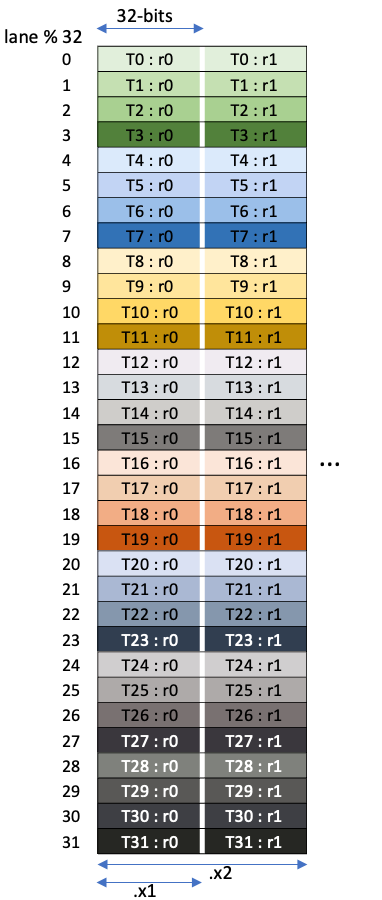
\includegraphics[width=0.3\textwidth]{figures/tikz/wp-tcgen05-tmem-fragment-3232b.png}
    \caption{\texttt{tcgen05\{.ld,.st\}.32x32b.\{x1,x2\}}}
    \label{fig:tmem_fragment-32x32}
\end{subfigure}
\hfill
\begin{subfigure}[b]{0.45\textwidth}
    \centering
    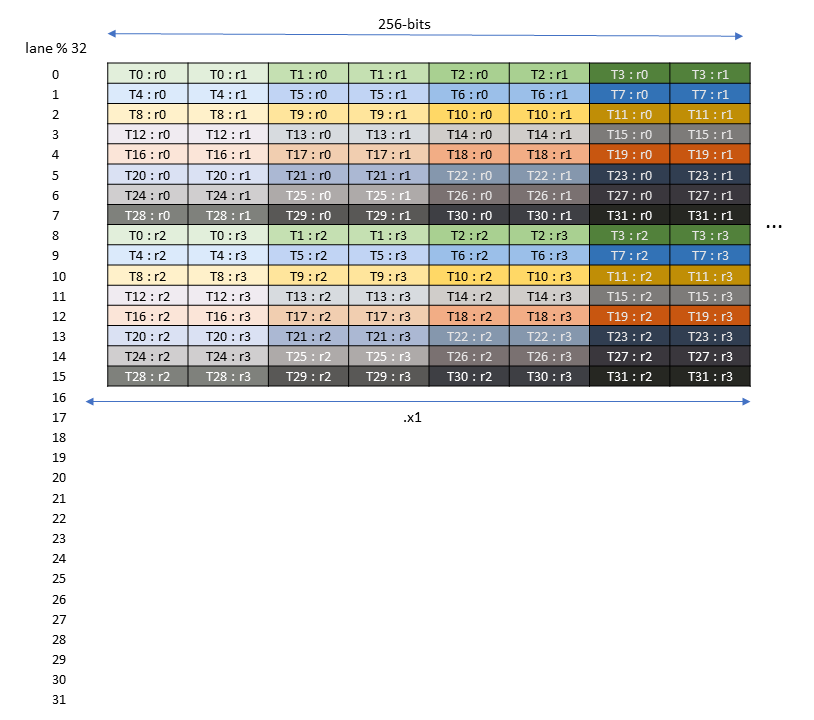
\includegraphics[width=0.8\textwidth]{figures/tikz/wp-tcgen05-tmem-fragment-16256b.png}
    \caption{\texttt{tcgen05\{.ld,.st\}.16x256b.x1}}
    \label{fig:tmem-fragment-16x256}
\end{subfigure}
\caption{TMEM load/store 指令访问特定的偏移，并将数据分配到线程本地寄存器（NVIDIA Corporation 2025）。}
\label{fig:tmem-fragments}
\end{figure}

向 Blackwell 的“张量内存”（tensor memory，TMEM）加载以及从其存储数据所使用的指令，会以一组预定义的固定偏移访问 TMEM，如图~\ref{fig:tmem-fragments} 所示。物理 TMEM 的编址是一个二维网格，最多包含 512 个“列”（col）与 128 个“通道”（lane）。图中是每条指令单个 warp 的访问模式；每条指令实际使用四个 warp，上述模式每 32 个通道重复一次、共重复四次。在对物理 TMEM 编址时，沿 32 位的“列”方向跨越一步使 TMEM 地址增加 1，沿“通道”方向向下跨越一步使 TMEM 地址增加 16384。基于这一物理编址，我们定义记录每条指令所访问的全部物理偏移的布局：
\begin{center}
\begin{tabular}{l | r@{:}l}
\quad\quad\quad\quad \textbf{指令} & \multicolumn{2}{c}{$(\text{指令 COL}, \text{指令 LANE}) \to \text{TMEM 偏移}$} \\
\hline
\texttt{tcgen05\{.ld,.st\}.32x32b.x1} & $(1,128)$ & $(1,16384)$ \\
\texttt{tcgen05\{.ld,.st\}.32x32b.x2} & $(2,128)$ & $(1,16384)$ \\
\texttt{tcgen05\{.ld,.st\}.16x256b.x1} & $(8,(16,4))$ & $(1,(16384,32\cdot 16384))$ \\
\end{tabular}
\end{center}
这些布局与具体指令一一对应，可用来精确确定每条指令将访问 TMEM 中的哪些偏移。

尽管 TMEM 采用二维编址，并被用作形状为 $(M,N)$ 的 MMA 的累加器，TMEM 的“通道”与“列”并不总与逻辑矩阵的行和列相对应。与任何编址方式一样，物理偏移可以通过任意的 \CuTe{} 布局被回绕并折叠成任意形状。因此，给定一个数据布局与一条 TMEM 指令，我们希望确定
\begin{enumerate}[itemsep=0pt,topsep=2pt]
\item 数据布局是否包含该指令将访问的全部偏移；以及
\item 指令所访问的偏移在数据布局中位于何处（以逻辑坐标表示）。
\end{enumerate}

一般地，设数据布局 $\v{A} : \Z(\v{A}) \to \Z_\alpha$ 将逻辑坐标映射到数据偏移，指令布局 $\v{T} : \Z(\v{T}) \to \Z_\beta$ 将指令坐标映射到数据偏移，我们希望确定所有偏移 $\v{T}(i)$ 在 $\v{A}$ 的像中的存在性及其位置。将其表述为
\begin{align*}
\forall i \in \Z_{\abs{\v{T}}}, \exists c \in \Z(\v{A}) \ \ s.t. \ \ \v{T}(i) = \v{A}(c)
\end{align*}
该问题可以通过计算 $\v{A}$ 的左逆并检验下式来高效求解：
\begin{align*}
\v{A}(\v{A}^\dagger(\v{T}(i))) = \v{T}(i)
\end{align*}
也就是说，
\begin{compactitem}
\item 所有偏移 $\v{T}(i)$ 都在 $\v{A}^\dagger$ 的定义域中。
\item 所有坐标 $\v{A}^\dagger(\v{T}(i))$ 都互不相同，且都在 $\v{A}$ 的定义域中。
\end{compactitem}
在这些条件下，我们可以断言：每个偏移 $\v{T}(i)$ 都出现在 $\v{A}$ 的像中，且位于坐标 $\v{A}^\dagger(\v{T}(i))$ 处。布局 $\v{A}^\dagger \circ \v{T}$ 把指令坐标映射到逻辑数据坐标，例如可借助 {\tt zipped\_divide} 把数据布局 $\v{A}$ 切分为与该指令所访问偏移相对应的若干子布局。

%% wp7 补布局、逻辑乘积/逻辑切分、结论与致谢（论文收尾）
\wpsh{补}
\label{sec:complement}

布局（layout）$\v{L} : \Z(\v{L}) \to \D$ 的\emph{补}（complement）是一个满足下列条件的布局 $\v{L}^* : \Z(\v{L}^*) \to \D$
\begin{align}
\label{eqn:comp:congruence}
\text{与陪域弱同余：} && \D \lesssim \v{L}^*, \\
\label{eqn:comp:disjoint}
\text{像互不相交：} && \forall b \in \Z(\v{L}), \ \forall a \in \Z^{\v{L}^*}/\{0\}, \ &\v{L}(b) \neq \v{L}^*(a), \\
\label{eqn:comp:ordered}
\text{像有序：} && \forall a \in \Z_{\abs{\v{L}^*}}/\{0\}, \ &\v{L}^*(a-1) < \v{L}^*(a).
%\text{\emph{???:}} && \v{L}^\dagger (\v{L}, \v{L}^*) \v{L}^\dagger = \v{L}^\dagger
\end{align}
布局的补是一个在原布局的陪域（codomain）之中、但不在其像（image）之中生成元素的布局。在复合（Composition）中，布局 $\v{L}$ 常被用作对另一个布局的间接寻址，因此补 $\v{L}^*$ 就是指向 $\v{L}$ 所遗漏元素的布局。有了 {\tt complement}，就能经由\emph{逻辑切分}（logical divide）把布局切开（第~\ref{sec:logical_divide}~节），也能经由\emph{逻辑乘积}（logical product）把布局重复、扩展（第~\ref{sec:logical_product}~节）。

本节只关注陪域 $\D$ 为 {\tt HTuple}($\Z$) 的布局：即整数，或对某个轮廓 D 而言 $\D = \Z^D$ 的坐标。弱同余条件式~\eqref{eqn:comp:congruence} 因此成立。像互不相交条件（式~\eqref{eqn:comp:disjoint}）保证补所生成的值与原布局生成的值互不相同：原布局取的是有限定义域 $\Z(\v{L})$，补取的是无穷扩展定义域 $\Z^{\v{L}^*}$，因此无论补的形状被截断还是被扩展（例如通过与右侧的布局复合），它所生成的值始终与原布局不同。最后，像有序条件（式~\eqref{eqn:comp:ordered}）确立了补布局的唯一性。

表~\ref{tab:complements} 给出了补的若干例子。

\begin{table}[ht]
\begin{center}
\begin{tabular}{|>{$}c<{$}|>{$}c<{$}|c|}
\v{L} & \v{L}^* & 备注 \\ \hline \hline
(4,8):(1,4) & 1:32 & 注意 $\forall i \in \Z^+, \v{L}^*(i) > \max_{j \in \Z_\v{L}} \v{L}(j)$。 \\ \hline
(4,8):(8,1) & 1:32 & 输入的顺序无关紧要。 \\ \hline
(4,(4,2)):(4,(1,16)) & 1:32 & 输入的层级结构无关紧要。 \\ \hline
(4,8):(1,5) & 1:40 \\ \hline
(4,8):(1,8) & (2,1):(4,64) & 仍然互不相交，但在陪域中“填补空洞”。 \\ \hline
((2,2),(2,4)):((0,1),(0,2)) & 1:8 & 步幅（stride）为 0 的模无贡献。 \\ \hline
((2,2),(2,4)):((0,2),(0,4)) & (2,1):(1,16) \\ \hline
(4,8):(e_0,e_1) & (1,1):(4e_0,8e_1) & 结果定义域与陪域 $\Z^{(\ast,\ast)}$ 同余。 \\ \hline
(4,(4,2)):(e_1,(e_0,12e_1)) & (1,(3,1)):(4e_0,(4e_1,24e_1)) & 弱同余、互不相交且有序。 \\ \hline
\end{tabular}
\end{center}
\caption{布局补的例子。}
\label{tab:complements}
\end{table}

\wpssh{应用：逻辑乘积}
\label{sec:logical_product}

两个布局 $\v{A}$ 与 $\v{B}$ 的逻辑乘积是一个布局 $\v{R}$，其中“布局 $\v{B}$ 的每个元素都被替换为布局 $\v{A}$ 的一个经过唯一平移的版本”。

具体地，我们将逻辑乘积定义为从两个布局产生 2 阶（rank-2）布局的函数
\begin{align*}
\v{A} \otimes \v{B} = (\v{A}, \v{A}^* \circ \v{B})
\end{align*}
其中 $\v{A}^*$ 是 $\v{A}$ 的补。结果的第一个模（mode）就是输入布局 $\v{A}$，而第二个模在元素形状（shape）与元素顺序上与输入布局 $\v{B}$ 相容。第一个模（即 $\v{A}$）通常被称为“块”，在“网格”布局 $\v{B}$ 上被重复。%Because the purpose of the logical product is to expand the domain and codomain of $\v{A}$, this does not require that $(\v{A},\v{A}^*)$ is surjective onto $\Z_{\norm{\v{B}}}$.

考虑这样的例子：行主序（row-major）布局 $(\textcolor{red}{3},\textcolor{red}{4}):(\textcolor{red}{4},\textcolor{red}{1})$ 块，要在列主序（col-major）布局 $(\textcolor{blue}{2},\textcolor{blue}{5}):(\textcolor{blue}{1},\textcolor{blue}{2})$ 网格中复现：
\begin{align*}
\begin{array}{cc} (\textcolor{red}{3}, & \textcolor{red}{4}) \\ (\textcolor{red}{4}, & \textcolor{red}{1}) \end{array}
\ \otimes \
\begin{array}{cc} (\textcolor{blue}{2}, & \textcolor{blue}{5}) \\ (\textcolor{blue}{1}, & \textcolor{blue}{2}) \end{array}
\ =\
\left(
\begin{array}{cc} (\textcolor{red}{3}, & \textcolor{red}{4}) \\ (\textcolor{red}{4}, & \textcolor{red}{1}) \end{array}, \
\begin{array}{c} 1 \\ 12 \end{array}
\ \circ \
\begin{array}{cc}(\textcolor{blue}{2}, & \textcolor{blue}{5}) \\ (\textcolor{blue}{1},& \textcolor{blue}{2}) \end{array}
\right)
\ = \
\begin{array}{cccc}((\textcolor{red}{3}, & \textcolor{red}{4}), & (\textcolor{blue}{2}, & \textcolor{blue}{5})) \\ ((\textcolor{red}{4}, & \textcolor{red}{1}), & (\textcolor{blue}{12}, & \textcolor{blue}{24})) \end{array}
\end{align*}
其中布局 $1:12$ 是 $(\textcolor{red}{3},\textcolor{red}{4}):(\textcolor{red}{4},\textcolor{red}{1})$ 的补。结果的第一个模中可以直接得到原始块，而第二个模以 $2\times 5$ 列主序的顺序把原始块铺 10 次，互不重叠。

再换一个例子，考虑布局 $(\textcolor{red}{4},\textcolor{red}{8}):(\textcolor{red}{20},\textcolor{red}{2})$ 块在行主序布局 $(\textcolor{blue}{3},\textcolor{blue}{2}):(\textcolor{blue}{2},\textcolor{blue}{1})$ 网格中复现：
\begin{align*}
\begin{array}{cc} (\textcolor{red}{4}, & \textcolor{red}{8}) \\ (\textcolor{red}{20}, & \textcolor{red}{2}) \end{array}
\ \otimes \
\begin{array}{cc} (\textcolor{blue}{3}, & \textcolor{blue}{2}) \\ (\textcolor{blue}{2}, & \textcolor{blue}{1}) \end{array}
\ = \
\left(
\begin{array}{cc} (\textcolor{red}{4}, & \textcolor{red}{8}) \\ (\textcolor{red}{20}, & \textcolor{red}{2}) \end{array}, \
\begin{array}{cc} (2, & 1) \\ (1, & 80) \end{array}
\ \circ \
\begin{array}{cc} (\textcolor{blue}{3}, & \textcolor{blue}{2}) \\ (\textcolor{blue}{2}, & \textcolor{blue}{1}) \end{array}
\right)
\ = \
\begin{array}{cccc}((\textcolor{red}{4}, & \textcolor{red}{8}), & (\textcolor{blue}{3}, & \textcolor{blue}{2})) \\ ((\textcolor{red}{20}, & \textcolor{red}{2}), & (\textcolor{blue}{80}, & \textcolor{blue}{1})) \end{array}
\end{align*}
其中布局 $(2,1):(1,80)$ 是 $(\textcolor{red}{4},\textcolor{red}{8}):(\textcolor{red}{20},\textcolor{red}{2})$ 的补。此时网格交错排布这些块，以产生结果的最小陪域。补布局决定结果如何为布局 $\v{B}$ 设定步幅，而布局 $\v{B}$ 决定结果如何为补布局排序并定形。

\paragraph{相关乘积}

逻辑乘积产生一个 2 阶布局，其中第一个模是原始块，第二个模被解释为该块的网格，即“分块”。

逻辑乘积对 $\v{A}$ 与 $\v{B}$ 的阶（rank）和相容性都没有限制；操作 {\tt blocked\_product} 则更直观，它利用输入的阶来构造结果的形状。直觉上，一个 $3 {\times} 4$ 布局与一个 $2 {\times} 5$ 布局相乘，就该得到一个 $6 {\times} 20$ 布局。{\tt blocked\_product} 要求 $\v{A}$ 与 $\v{B}$ 的阶相同，
\begin{align*}
\text{阶}(\v{A}) = \text{阶}(\v{B})
\end{align*}
以便施加一个 zip 操作，把逻辑上的行模与行模、列模与列模组合起来。例如，将上例中的模重排
\begin{align*}
\begin{array}{cccc}((\textcolor{red}{3}, & \textcolor{red}{4}), & (\textcolor{blue}{2}, & \textcolor{blue}{5})) \\ ((\textcolor{red}{4}, & \textcolor{red}{1}), & (\textcolor{blue}{12}, & \textcolor{blue}{24})) \end{array}
\ \Longrightarrow \
\begin{array}{cccc}((\textcolor{red}{3}, & \textcolor{blue}{2}), & (\textcolor{red}{4}, & \textcolor{blue}{5})) \\ ((\textcolor{red}{4}, & \textcolor{blue}{12}), & (\textcolor{red}{1}, & \textcolor{blue}{24})) \end{array}
\end{align*}
便得到一个 $6 {\times} 20$ 布局。图~\ref{fig:blockedproduct} 画出了这个布局，其中每个 $3 {\times} 4$ 块都施以底纹。“块状”之名由此而来：结果布局中的每个 $3 {\times} 4$ 块，都是原始 $3 {\times} 4$ 块的平移版本。

\begin{figure}[ht]
\centering
%\includegraphics[scale=0.5]{blocked_product}
\scalebox{0.5}{
\begin{tikzpicture}[x={(0cm,-1cm)},y={(1cm,0cm)},every node/.style={minimum size=1cm, outer sep=0pt}]
\node[fill={rgb,255:red,255;green,255;blue,255}] at (0,0) {\large 0};
\node[fill={rgb,255:red,255;green,255;blue,255}] at (0,1) {\large 1};
\node[fill={rgb,255:red,255;green,255;blue,255}] at (0,2) {\large 2};
\node[fill={rgb,255:red,255;green,255;blue,255}] at (0,3) {\large 3};
\node[fill={rgb,255:red,210;green,210;blue,255}] at (0,4) {\large 24};
\node[fill={rgb,255:red,210;green,210;blue,255}] at (0,5) {\large 25};
\node[fill={rgb,255:red,210;green,210;blue,255}] at (0,6) {\large 26};
\node[fill={rgb,255:red,210;green,210;blue,255}] at (0,7) {\large 27};
\node[fill={rgb,255:red,210;green,255;blue,210}] at (0,8) {\large 48};
\node[fill={rgb,255:red,210;green,255;blue,210}] at (0,9) {\large 49};
\node[fill={rgb,255:red,210;green,255;blue,210}] at (0,10) {\large 50};
\node[fill={rgb,255:red,210;green,255;blue,210}] at (0,11) {\large 51};
\node[fill={rgb,255:red,255;green,255;blue,210}] at (0,12) {\large 72};
\node[fill={rgb,255:red,255;green,255;blue,210}] at (0,13) {\large 73};
\node[fill={rgb,255:red,255;green,255;blue,210}] at (0,14) {\large 74};
\node[fill={rgb,255:red,255;green,255;blue,210}] at (0,15) {\large 75};
\node[fill={rgb,255:red,255;green,210;blue,210}] at (0,16) {\large 96};
\node[fill={rgb,255:red,255;green,210;blue,210}] at (0,17) {\large 97};
\node[fill={rgb,255:red,255;green,210;blue,210}] at (0,18) {\large 98};
\node[fill={rgb,255:red,255;green,210;blue,210}] at (0,19) {\large 99};
\node[fill={rgb,255:red,255;green,255;blue,255}] at (1,0) {\large 4};
\node[fill={rgb,255:red,255;green,255;blue,255}] at (1,1) {\large 5};
\node[fill={rgb,255:red,255;green,255;blue,255}] at (1,2) {\large 6};
\node[fill={rgb,255:red,255;green,255;blue,255}] at (1,3) {\large 7};
\node[fill={rgb,255:red,210;green,210;blue,255}] at (1,4) {\large 28};
\node[fill={rgb,255:red,210;green,210;blue,255}] at (1,5) {\large 29};
\node[fill={rgb,255:red,210;green,210;blue,255}] at (1,6) {\large 30};
\node[fill={rgb,255:red,210;green,210;blue,255}] at (1,7) {\large 31};
\node[fill={rgb,255:red,210;green,255;blue,210}] at (1,8) {\large 52};
\node[fill={rgb,255:red,210;green,255;blue,210}] at (1,9) {\large 53};
\node[fill={rgb,255:red,210;green,255;blue,210}] at (1,10) {\large 54};
\node[fill={rgb,255:red,210;green,255;blue,210}] at (1,11) {\large 55};
\node[fill={rgb,255:red,255;green,255;blue,210}] at (1,12) {\large 76};
\node[fill={rgb,255:red,255;green,255;blue,210}] at (1,13) {\large 77};
\node[fill={rgb,255:red,255;green,255;blue,210}] at (1,14) {\large 78};
\node[fill={rgb,255:red,255;green,255;blue,210}] at (1,15) {\large 79};
\node[fill={rgb,255:red,255;green,210;blue,210}] at (1,16) {\large 100};
\node[fill={rgb,255:red,255;green,210;blue,210}] at (1,17) {\large 101};
\node[fill={rgb,255:red,255;green,210;blue,210}] at (1,18) {\large 102};
\node[fill={rgb,255:red,255;green,210;blue,210}] at (1,19) {\large 103};
\node[fill={rgb,255:red,255;green,255;blue,255}] at (2,0) {\large 8};
\node[fill={rgb,255:red,255;green,255;blue,255}] at (2,1) {\large 9};
\node[fill={rgb,255:red,255;green,255;blue,255}] at (2,2) {\large 10};
\node[fill={rgb,255:red,255;green,255;blue,255}] at (2,3) {\large 11};
\node[fill={rgb,255:red,210;green,210;blue,255}] at (2,4) {\large 32};
\node[fill={rgb,255:red,210;green,210;blue,255}] at (2,5) {\large 33};
\node[fill={rgb,255:red,210;green,210;blue,255}] at (2,6) {\large 34};
\node[fill={rgb,255:red,210;green,210;blue,255}] at (2,7) {\large 35};
\node[fill={rgb,255:red,210;green,255;blue,210}] at (2,8) {\large 56};
\node[fill={rgb,255:red,210;green,255;blue,210}] at (2,9) {\large 57};
\node[fill={rgb,255:red,210;green,255;blue,210}] at (2,10) {\large 58};
\node[fill={rgb,255:red,210;green,255;blue,210}] at (2,11) {\large 59};
\node[fill={rgb,255:red,255;green,255;blue,210}] at (2,12) {\large 80};
\node[fill={rgb,255:red,255;green,255;blue,210}] at (2,13) {\large 81};
\node[fill={rgb,255:red,255;green,255;blue,210}] at (2,14) {\large 82};
\node[fill={rgb,255:red,255;green,255;blue,210}] at (2,15) {\large 83};
\node[fill={rgb,255:red,255;green,210;blue,210}] at (2,16) {\large 104};
\node[fill={rgb,255:red,255;green,210;blue,210}] at (2,17) {\large 105};
\node[fill={rgb,255:red,255;green,210;blue,210}] at (2,18) {\large 106};
\node[fill={rgb,255:red,255;green,210;blue,210}] at (2,19) {\large 107};
\node[fill={rgb,255:red,175;green,175;blue,175}] at (3,0) {\large 12};
\node[fill={rgb,255:red,175;green,175;blue,175}] at (3,1) {\large 13};
\node[fill={rgb,255:red,175;green,175;blue,175}] at (3,2) {\large 14};
\node[fill={rgb,255:red,175;green,175;blue,175}] at (3,3) {\large 15};
\node[fill={rgb,255:red,175;green,175;blue,255}] at (3,4) {\large 36};
\node[fill={rgb,255:red,175;green,175;blue,255}] at (3,5) {\large 37};
\node[fill={rgb,255:red,175;green,175;blue,255}] at (3,6) {\large 38};
\node[fill={rgb,255:red,175;green,175;blue,255}] at (3,7) {\large 39};
\node[fill={rgb,255:red,175;green,255;blue,175}] at (3,8) {\large 60};
\node[fill={rgb,255:red,175;green,255;blue,175}] at (3,9) {\large 61};
\node[fill={rgb,255:red,175;green,255;blue,175}] at (3,10) {\large 62};
\node[fill={rgb,255:red,175;green,255;blue,175}] at (3,11) {\large 63};
\node[fill={rgb,255:red,255;green,255;blue,175}] at (3,12) {\large 84};
\node[fill={rgb,255:red,255;green,255;blue,175}] at (3,13) {\large 85};
\node[fill={rgb,255:red,255;green,255;blue,175}] at (3,14) {\large 86};
\node[fill={rgb,255:red,255;green,255;blue,175}] at (3,15) {\large 87};
\node[fill={rgb,255:red,255;green,175;blue,175}] at (3,16) {\large 108};
\node[fill={rgb,255:red,255;green,175;blue,175}] at (3,17) {\large 109};
\node[fill={rgb,255:red,255;green,175;blue,175}] at (3,18) {\large 110};
\node[fill={rgb,255:red,255;green,175;blue,175}] at (3,19) {\large 111};
\node[fill={rgb,255:red,175;green,175;blue,175}] at (4,0) {\large 16};
\node[fill={rgb,255:red,175;green,175;blue,175}] at (4,1) {\large 17};
\node[fill={rgb,255:red,175;green,175;blue,175}] at (4,2) {\large 18};
\node[fill={rgb,255:red,175;green,175;blue,175}] at (4,3) {\large 19};
\node[fill={rgb,255:red,175;green,175;blue,255}] at (4,4) {\large 40};
\node[fill={rgb,255:red,175;green,175;blue,255}] at (4,5) {\large 41};
\node[fill={rgb,255:red,175;green,175;blue,255}] at (4,6) {\large 42};
\node[fill={rgb,255:red,175;green,175;blue,255}] at (4,7) {\large 43};
\node[fill={rgb,255:red,175;green,255;blue,175}] at (4,8) {\large 64};
\node[fill={rgb,255:red,175;green,255;blue,175}] at (4,9) {\large 65};
\node[fill={rgb,255:red,175;green,255;blue,175}] at (4,10) {\large 66};
\node[fill={rgb,255:red,175;green,255;blue,175}] at (4,11) {\large 67};
\node[fill={rgb,255:red,255;green,255;blue,175}] at (4,12) {\large 88};
\node[fill={rgb,255:red,255;green,255;blue,175}] at (4,13) {\large 89};
\node[fill={rgb,255:red,255;green,255;blue,175}] at (4,14) {\large 90};
\node[fill={rgb,255:red,255;green,255;blue,175}] at (4,15) {\large 91};
\node[fill={rgb,255:red,255;green,175;blue,175}] at (4,16) {\large 112};
\node[fill={rgb,255:red,255;green,175;blue,175}] at (4,17) {\large 113};
\node[fill={rgb,255:red,255;green,175;blue,175}] at (4,18) {\large 114};
\node[fill={rgb,255:red,255;green,175;blue,175}] at (4,19) {\large 115};
\node[fill={rgb,255:red,175;green,175;blue,175}] at (5,0) {\large 20};
\node[fill={rgb,255:red,175;green,175;blue,175}] at (5,1) {\large 21};
\node[fill={rgb,255:red,175;green,175;blue,175}] at (5,2) {\large 22};
\node[fill={rgb,255:red,175;green,175;blue,175}] at (5,3) {\large 23};
\node[fill={rgb,255:red,175;green,175;blue,255}] at (5,4) {\large 44};
\node[fill={rgb,255:red,175;green,175;blue,255}] at (5,5) {\large 45};
\node[fill={rgb,255:red,175;green,175;blue,255}] at (5,6) {\large 46};
\node[fill={rgb,255:red,175;green,175;blue,255}] at (5,7) {\large 47};
\node[fill={rgb,255:red,175;green,255;blue,175}] at (5,8) {\large 68};
\node[fill={rgb,255:red,175;green,255;blue,175}] at (5,9) {\large 69};
\node[fill={rgb,255:red,175;green,255;blue,175}] at (5,10) {\large 70};
\node[fill={rgb,255:red,175;green,255;blue,175}] at (5,11) {\large 71};
\node[fill={rgb,255:red,255;green,255;blue,175}] at (5,12) {\large 92};
\node[fill={rgb,255:red,255;green,255;blue,175}] at (5,13) {\large 93};
\node[fill={rgb,255:red,255;green,255;blue,175}] at (5,14) {\large 94};
\node[fill={rgb,255:red,255;green,255;blue,175}] at (5,15) {\large 95};
\node[fill={rgb,255:red,255;green,175;blue,175}] at (5,16) {\large 116};
\node[fill={rgb,255:red,255;green,175;blue,175}] at (5,17) {\large 117};
\node[fill={rgb,255:red,255;green,175;blue,175}] at (5,18) {\large 118};
\node[fill={rgb,255:red,255;green,175;blue,175}] at (5,19) {\large 119};
\draw[color=black,thick,shift={(-0.5,-0.5)}] (0,0) grid (6,20);

\node at (0,-1) {\Large{\texttt{0}}};
\node at (1,-1) {\Large{\texttt{1}}};
\node at (2,-1) {\Large{\texttt{2}}};
\node at (3,-1) {\Large{\texttt{3}}};
\node at (4,-1) {\Large{\texttt{4}}};
\node at (5,-1) {\Large{\texttt{5}}};
\node at (-1,0) {\Large{\texttt{0}}};
\node at (-1,1) {\Large{\texttt{1}}};
\node at (-1,2) {\Large{\texttt{2}}};
\node at (-1,3) {\Large{\texttt{3}}};
\node at (-1,4) {\Large{\texttt{4}}};
\node at (-1,5) {\Large{\texttt{5}}};
\node at (-1,6) {\Large{\texttt{6}}};
\node at (-1,7) {\Large{\texttt{7}}};
\node at (-1,8) {\Large{\texttt{8}}};
\node at (-1,9) {\Large{\texttt{9}}};
\node at (-1,10) {\Large{\texttt{10}}};
\node at (-1,11) {\Large{\texttt{11}}};
\node at (-1,12) {\Large{\texttt{12}}};
\node at (-1,13) {\Large{\texttt{13}}};
\node at (-1,14) {\Large{\texttt{14}}};
\node at (-1,15) {\Large{\texttt{15}}};
\node at (-1,16) {\Large{\texttt{16}}};
\node at (-1,17) {\Large{\texttt{17}}};
\node at (-1,18) {\Large{\texttt{18}}};
\node at (-1,19) {\Large{\texttt{19}}};
\end{tikzpicture}
}
\caption{行主序 $(3,4):(4,1)$ 块与列主序 $(2,5):(1,2)$ 分块的 {\tt blocked\_product}。}
\label{fig:blockedproduct}
\end{figure}

操作 {\tt raked\_product} 与块状乘积类似，只是各模以相反的顺序拉链（zip）组合：
\begin{align*}
\begin{array}{cccc}((\textcolor{red}{3}, & \textcolor{red}{4}), & (\textcolor{blue}{2}, & \textcolor{blue}{5})) \\ ((\textcolor{red}{4}, & \textcolor{red}{1}), & (\textcolor{blue}{12}, & \textcolor{blue}{24})) \end{array}
\ \Longrightarrow \
\begin{array}{cccc}((\textcolor{blue}{2}, & \textcolor{red}{3}), & (\textcolor{blue}{5}, & \textcolor{red}{4})) \\ ((\textcolor{blue}{12}, & \textcolor{red}{4}), & (\textcolor{blue}{24}, & \textcolor{red}{1})) \end{array}
\end{align*}
其效果是 $3 {\times} 4$ 块被“耙”（raked）在 $2 {\times} 5$ 块之上，而非“块状”排布。图~\ref{fig:rakedproduct} 画出了得到的布局，其中每个 $3 {\times} 4$ 块都施以底纹。

\begin{figure}[ht]
\centering
%\includegraphics[scale=0.5]{raked_product}
\scalebox{0.5}{
\begin{tikzpicture}[x={(0cm,-1cm)},y={(1cm,0cm)},every node/.style={minimum size=1cm, outer sep=0pt}]

\node[fill={rgb,255:red,255;green,255;blue,255}] at (0,0) {\large 0};
\node[fill={rgb,255:red,210;green,210;blue,255}] at (0,1) {\large 24};
\node[fill={rgb,255:red,210;green,255;blue,210}] at (0,2) {\large 48};
\node[fill={rgb,255:red,255;green,255;blue,210}] at (0,3) {\large 72};
\node[fill={rgb,255:red,255;green,210;blue,210}] at (0,4) {\large 96};
\node[fill={rgb,255:red,255;green,255;blue,255}] at (0,5) {\large 1};
\node[fill={rgb,255:red,210;green,210;blue,255}] at (0,6) {\large 25};
\node[fill={rgb,255:red,210;green,255;blue,210}] at (0,7) {\large 49};
\node[fill={rgb,255:red,255;green,255;blue,210}] at (0,8) {\large 73};
\node[fill={rgb,255:red,255;green,210;blue,210}] at (0,9) {\large 97};
\node[fill={rgb,255:red,255;green,255;blue,255}] at (0,10) {\large 2};
\node[fill={rgb,255:red,210;green,210;blue,255}] at (0,11) {\large 26};
\node[fill={rgb,255:red,210;green,255;blue,210}] at (0,12) {\large 50};
\node[fill={rgb,255:red,255;green,255;blue,210}] at (0,13) {\large 74};
\node[fill={rgb,255:red,255;green,210;blue,210}] at (0,14) {\large 98};
\node[fill={rgb,255:red,255;green,255;blue,255}] at (0,15) {\large 3};
\node[fill={rgb,255:red,210;green,210;blue,255}] at (0,16) {\large 27};
\node[fill={rgb,255:red,210;green,255;blue,210}] at (0,17) {\large 51};
\node[fill={rgb,255:red,255;green,255;blue,210}] at (0,18) {\large 75};
\node[fill={rgb,255:red,255;green,210;blue,210}] at (0,19) {\large 99};
\node[fill={rgb,255:red,175;green,175;blue,175}] at (1,0) {\large 12};
\node[fill={rgb,255:red,175;green,175;blue,255}] at (1,1) {\large 36};
\node[fill={rgb,255:red,175;green,255;blue,175}] at (1,2) {\large 60};
\node[fill={rgb,255:red,255;green,255;blue,175}] at (1,3) {\large 84};
\node[fill={rgb,255:red,255;green,175;blue,175}] at (1,4) {\large 108};
\node[fill={rgb,255:red,175;green,175;blue,175}] at (1,5) {\large 13};
\node[fill={rgb,255:red,175;green,175;blue,255}] at (1,6) {\large 37};
\node[fill={rgb,255:red,175;green,255;blue,175}] at (1,7) {\large 61};
\node[fill={rgb,255:red,255;green,255;blue,175}] at (1,8) {\large 85};
\node[fill={rgb,255:red,255;green,175;blue,175}] at (1,9) {\large 109};
\node[fill={rgb,255:red,175;green,175;blue,175}] at (1,10) {\large 14};
\node[fill={rgb,255:red,175;green,175;blue,255}] at (1,11) {\large 38};
\node[fill={rgb,255:red,175;green,255;blue,175}] at (1,12) {\large 62};
\node[fill={rgb,255:red,255;green,255;blue,175}] at (1,13) {\large 86};
\node[fill={rgb,255:red,255;green,175;blue,175}] at (1,14) {\large 110};
\node[fill={rgb,255:red,175;green,175;blue,175}] at (1,15) {\large 15};
\node[fill={rgb,255:red,175;green,175;blue,255}] at (1,16) {\large 39};
\node[fill={rgb,255:red,175;green,255;blue,175}] at (1,17) {\large 63};
\node[fill={rgb,255:red,255;green,255;blue,175}] at (1,18) {\large 87};
\node[fill={rgb,255:red,255;green,175;blue,175}] at (1,19) {\large 111};
\node[fill={rgb,255:red,255;green,255;blue,255}] at (2,0) {\large 4};
\node[fill={rgb,255:red,210;green,210;blue,255}] at (2,1) {\large 28};
\node[fill={rgb,255:red,210;green,255;blue,210}] at (2,2) {\large 52};
\node[fill={rgb,255:red,255;green,255;blue,210}] at (2,3) {\large 76};
\node[fill={rgb,255:red,255;green,210;blue,210}] at (2,4) {\large 100};
\node[fill={rgb,255:red,255;green,255;blue,255}] at (2,5) {\large 5};
\node[fill={rgb,255:red,210;green,210;blue,255}] at (2,6) {\large 29};
\node[fill={rgb,255:red,210;green,255;blue,210}] at (2,7) {\large 53};
\node[fill={rgb,255:red,255;green,255;blue,210}] at (2,8) {\large 77};
\node[fill={rgb,255:red,255;green,210;blue,210}] at (2,9) {\large 101};
\node[fill={rgb,255:red,255;green,255;blue,255}] at (2,10) {\large 6};
\node[fill={rgb,255:red,210;green,210;blue,255}] at (2,11) {\large 30};
\node[fill={rgb,255:red,210;green,255;blue,210}] at (2,12) {\large 54};
\node[fill={rgb,255:red,255;green,255;blue,210}] at (2,13) {\large 78};
\node[fill={rgb,255:red,255;green,210;blue,210}] at (2,14) {\large 102};
\node[fill={rgb,255:red,255;green,255;blue,255}] at (2,15) {\large 7};
\node[fill={rgb,255:red,210;green,210;blue,255}] at (2,16) {\large 31};
\node[fill={rgb,255:red,210;green,255;blue,210}] at (2,17) {\large 55};
\node[fill={rgb,255:red,255;green,255;blue,210}] at (2,18) {\large 79};
\node[fill={rgb,255:red,255;green,210;blue,210}] at (2,19) {\large 103};
\node[fill={rgb,255:red,175;green,175;blue,175}] at (3,0) {\large 16};
\node[fill={rgb,255:red,175;green,175;blue,255}] at (3,1) {\large 40};
\node[fill={rgb,255:red,175;green,255;blue,175}] at (3,2) {\large 64};
\node[fill={rgb,255:red,255;green,255;blue,175}] at (3,3) {\large 88};
\node[fill={rgb,255:red,255;green,175;blue,175}] at (3,4) {\large 112};
\node[fill={rgb,255:red,175;green,175;blue,175}] at (3,5) {\large 17};
\node[fill={rgb,255:red,175;green,175;blue,255}] at (3,6) {\large 41};
\node[fill={rgb,255:red,175;green,255;blue,175}] at (3,7) {\large 65};
\node[fill={rgb,255:red,255;green,255;blue,175}] at (3,8) {\large 89};
\node[fill={rgb,255:red,255;green,175;blue,175}] at (3,9) {\large 113};
\node[fill={rgb,255:red,175;green,175;blue,175}] at (3,10) {\large 18};
\node[fill={rgb,255:red,175;green,175;blue,255}] at (3,11) {\large 42};
\node[fill={rgb,255:red,175;green,255;blue,175}] at (3,12) {\large 66};
\node[fill={rgb,255:red,255;green,255;blue,175}] at (3,13) {\large 90};
\node[fill={rgb,255:red,255;green,175;blue,175}] at (3,14) {\large 114};
\node[fill={rgb,255:red,175;green,175;blue,175}] at (3,15) {\large 19};
\node[fill={rgb,255:red,175;green,175;blue,255}] at (3,16) {\large 43};
\node[fill={rgb,255:red,175;green,255;blue,175}] at (3,17) {\large 67};
\node[fill={rgb,255:red,255;green,255;blue,175}] at (3,18) {\large 91};
\node[fill={rgb,255:red,255;green,175;blue,175}] at (3,19) {\large 115};
\node[fill={rgb,255:red,255;green,255;blue,255}] at (4,0) {\large 8};
\node[fill={rgb,255:red,210;green,210;blue,255}] at (4,1) {\large 32};
\node[fill={rgb,255:red,210;green,255;blue,210}] at (4,2) {\large 56};
\node[fill={rgb,255:red,255;green,255;blue,210}] at (4,3) {\large 80};
\node[fill={rgb,255:red,255;green,210;blue,210}] at (4,4) {\large 104};
\node[fill={rgb,255:red,255;green,255;blue,255}] at (4,5) {\large 9};
\node[fill={rgb,255:red,210;green,210;blue,255}] at (4,6) {\large 33};
\node[fill={rgb,255:red,210;green,255;blue,210}] at (4,7) {\large 57};
\node[fill={rgb,255:red,255;green,255;blue,210}] at (4,8) {\large 81};
\node[fill={rgb,255:red,255;green,210;blue,210}] at (4,9) {\large 105};
\node[fill={rgb,255:red,255;green,255;blue,255}] at (4,10) {\large 10};
\node[fill={rgb,255:red,210;green,210;blue,255}] at (4,11) {\large 34};
\node[fill={rgb,255:red,210;green,255;blue,210}] at (4,12) {\large 58};
\node[fill={rgb,255:red,255;green,255;blue,210}] at (4,13) {\large 82};
\node[fill={rgb,255:red,255;green,210;blue,210}] at (4,14) {\large 106};
\node[fill={rgb,255:red,255;green,255;blue,255}] at (4,15) {\large 11};
\node[fill={rgb,255:red,210;green,210;blue,255}] at (4,16) {\large 35};
\node[fill={rgb,255:red,210;green,255;blue,210}] at (4,17) {\large 59};
\node[fill={rgb,255:red,255;green,255;blue,210}] at (4,18) {\large 83};
\node[fill={rgb,255:red,255;green,210;blue,210}] at (4,19) {\large 107};
\node[fill={rgb,255:red,175;green,175;blue,175}] at (5,0) {\large 20};
\node[fill={rgb,255:red,175;green,175;blue,255}] at (5,1) {\large 44};
\node[fill={rgb,255:red,175;green,255;blue,175}] at (5,2) {\large 68};
\node[fill={rgb,255:red,255;green,255;blue,175}] at (5,3) {\large 92};
\node[fill={rgb,255:red,255;green,175;blue,175}] at (5,4) {\large 116};
\node[fill={rgb,255:red,175;green,175;blue,175}] at (5,5) {\large 21};
\node[fill={rgb,255:red,175;green,175;blue,255}] at (5,6) {\large 45};
\node[fill={rgb,255:red,175;green,255;blue,175}] at (5,7) {\large 69};
\node[fill={rgb,255:red,255;green,255;blue,175}] at (5,8) {\large 93};
\node[fill={rgb,255:red,255;green,175;blue,175}] at (5,9) {\large 117};
\node[fill={rgb,255:red,175;green,175;blue,175}] at (5,10) {\large 22};
\node[fill={rgb,255:red,175;green,175;blue,255}] at (5,11) {\large 46};
\node[fill={rgb,255:red,175;green,255;blue,175}] at (5,12) {\large 70};
\node[fill={rgb,255:red,255;green,255;blue,175}] at (5,13) {\large 94};
\node[fill={rgb,255:red,255;green,175;blue,175}] at (5,14) {\large 118};
\node[fill={rgb,255:red,175;green,175;blue,175}] at (5,15) {\large 23};
\node[fill={rgb,255:red,175;green,175;blue,255}] at (5,16) {\large 47};
\node[fill={rgb,255:red,175;green,255;blue,175}] at (5,17) {\large 71};
\node[fill={rgb,255:red,255;green,255;blue,175}] at (5,18) {\large 95};
\node[fill={rgb,255:red,255;green,175;blue,175}] at (5,19) {\large 119};
\draw[color=black,thick,shift={(-0.5,-0.5)}] (0,0) grid (6,20);

\node at (0,-1) {\Large{\texttt{0}}};
\node at (1,-1) {\Large{\texttt{1}}};
\node at (2,-1) {\Large{\texttt{2}}};
\node at (3,-1) {\Large{\texttt{3}}};
\node at (4,-1) {\Large{\texttt{4}}};
\node at (5,-1) {\Large{\texttt{5}}};
\node at (-1,0) {\Large{\texttt{0}}};
\node at (-1,1) {\Large{\texttt{1}}};
\node at (-1,2) {\Large{\texttt{2}}};
\node at (-1,3) {\Large{\texttt{3}}};
\node at (-1,4) {\Large{\texttt{4}}};
\node at (-1,5) {\Large{\texttt{5}}};
\node at (-1,6) {\Large{\texttt{6}}};
\node at (-1,7) {\Large{\texttt{7}}};
\node at (-1,8) {\Large{\texttt{8}}};
\node at (-1,9) {\Large{\texttt{9}}};
\node at (-1,10) {\Large{\texttt{10}}};
\node at (-1,11) {\Large{\texttt{11}}};
\node at (-1,12) {\Large{\texttt{12}}};
\node at (-1,13) {\Large{\texttt{13}}};
\node at (-1,14) {\Large{\texttt{14}}};
\node at (-1,15) {\Large{\texttt{15}}};
\node at (-1,16) {\Large{\texttt{16}}};
\node at (-1,17) {\Large{\texttt{17}}};
\node at (-1,18) {\Large{\texttt{18}}};
\node at (-1,19) {\Large{\texttt{19}}};
\end{tikzpicture}
}
\caption{行主序 $(3,4):(4,1)$ 块与列主序 $(2,5):(1,2)$ 分块的 {\tt raked\_product}。}
\label{fig:rakedproduct}
\end{figure}

%The operation {\tt tiled\_product} is another convenience function that simply flattens by one level the second mode of a logical product.

逻辑乘积还有不少其他版本，都会对模额外分组与重排，让结果更便于使用。

\wpssh{应用：逻辑切分}
\label{sec:logical_divide}

两个布局 $\v{A}$ 与 $\v{B}$ 的逻辑切分是一个布局 $\v{R}$，其中“布局 $\v{A}$ 被一分为二：被 $\v{B}$ 指向的元素与未被 $\v{B}$ 指向的元素”。

具体地，我们将逻辑切分定义为从两个布局产生 2 阶布局的函数
\begin{align*}
\v{A} \oslash \v{B} = \v{A} \circ (\v{B}, \v{B}^*_{\abs{\v{A}}}) = \v{A} \circ \v{B}^\bigstar
\end{align*}
其中 $\v{B}^*_{\abs{\v{A}}}$ 是 $\v{B}$ 相对于布局 $\v{A}$ 的尺寸所取的补。这个操作要保留 $\v{A}$ 的全部元素、只是把布局 $\v{A}$ 一分为二，所以我们要求 $\v{B}^\bigstar = (\v{B},\v{B}^*_{\abs{\v{A}}})$ 满射到 $\Z_{\abs{A}}$。这通常要扩展 $\v{B}^*$ 的尺寸，使 $\abs{\v{B}^\bigstar} \geq \abs{\v{A}}$。我们还要求补 $\v{B}^*$ 在如下意义上“补全”布局 $\v{B}$：$\v{B}^\bigstar = (\v{B},\v{B}^*_{\abs{A}})$ 具有自反广义逆 $\v{B}^+$，满足
\begin{align}
\v{B}^\bigstar \v{B}^+ \v{B}^\bigstar = \v{B}^\bigstar \\
\v{B}^+ \v{B}^\bigstar \v{B}^+ = \v{B}^+
\end{align}

与逻辑乘积操作类似，结果布局 $\v{A} \circ \v{B}$ 的第一个模通常被称为“块”，它在“网格”（即“分块”）布局 $\v{A} \circ \v{B}^*_{\abs{\v{A}}}$ 上被重复。参数 $\v{B}$ 被称为“分块器”，它可以扩展到布局之外，详见第~\ref{sec:tiler}~节。

常见需求是从另一个布局中取出某组逻辑元素，比如每隔三个取一个，用复合就能做到：
\begin{align*}
\begin{array}{c} \textcolor{red}{24} \\ \textcolor{red}{3} \end{array}
\ \circ \
\begin{array}{c} \textcolor{blue}{8} \\ \textcolor{blue}{3} \end{array}
\ &= \
\begin{array}{c} \textcolor{blue}{8} \\ \textcolor{blue}{9} \end{array} \\
\begin{array}{ccc} (\textcolor{red}{6}, & \textcolor{red}{2}, & \textcolor{red}{2}) \\ (\textcolor{red}{2}, & \textcolor{red}{1}, & \textcolor{red}{20}) \end{array}
\ \circ \
\begin{array}{c} \textcolor{blue}{8} \\ \textcolor{blue}{3} \end{array}
\ &= \
\begin{array}{ccc} (\textcolor{blue}{2}, & \textcolor{blue}{2}, & \textcolor{blue}{2}) \\ (\textcolor{blue}{6}, & \textcolor{blue}{1}, & \textcolor{blue}{20}) \end{array}
\end{align*}
在上面两种情形中，都是 24 个元素的布局与布局 $8:3$ 复合，得到每隔三个取一个元素的布局。但左手边布局中“其余”的元素怎么办？逻辑切分把左手边的布局拆成两块：被右手边“命中”的部分与“其余”部分：
\begin{align*}
\begin{array}{c} \textcolor{red}{24} \\ \textcolor{red}{3} \end{array}
\ \oslash \
\begin{array}{c} \textcolor{blue}{8} \\ \textcolor{blue}{3} \end{array}
\ &=& \
\begin{array}{c} \textcolor{red}{24} \\ \textcolor{red}{3} \end{array}
\ \circ \
\begin{array}{cc} (\textcolor{blue}{8}, & 3) \\ (\textcolor{blue}{3}, & 1) \end{array}
\ &=& \
\begin{array}{cc} (\textcolor{blue}{8}, & 3) \\ (\textcolor{blue}{9}, & 3) \end{array} \\
\begin{array}{ccc} (\textcolor{red}{6}, & \textcolor{red}{2}, & \textcolor{red}{2}) \\ (\textcolor{red}{2}, & \textcolor{red}{1}, & \textcolor{red}{20}) \end{array}
\ \oslash \
\begin{array}{c} \textcolor{blue}{8} \\ \textcolor{blue}{3} \end{array}
\ &=& \
\begin{array}{ccc} (\textcolor{red}{6}, & \textcolor{red}{2}, & \textcolor{red}{2}) \\ (\textcolor{red}{2}, & \textcolor{red}{1}, & \textcolor{red}{20}) \end{array}
\ \circ \
\begin{array}{cc} (\textcolor{blue}{8}, & 3) \\ (\textcolor{blue}{3}, & 1) \end{array}
\ &=& \
\begin{array}{cccc} ((\textcolor{blue}{2}, & \textcolor{blue}{2}, & \textcolor{blue}{2}), & 3) \\ ((\textcolor{blue}{6}, & \textcolor{blue}{1}, & \textcolor{blue}{20}), & 2) \end{array}
\end{align*}
其中 $3:1$ 是 $8:3$ 在尺寸 24 之下的补。结果的第一模按要求仍然包含左手边布局中每隔三个取一个的元素，而结果的第二模是这些“块”在原布局中的个数（本例中为 3）以及这些块之间的步幅。补用来确定缺失了哪些元素、以何种顺序保留它们。

\paragraph{相关切分}

与复合类似，逻辑切分也经常按模来做，沿用同样的记号与策略
\begin{align*}
\v{A} \oslash \langle \v{B},\v{C} \rangle = (\v{A}_0,\v{A}_1) \oslash \langle \v{B},\v{C} \rangle = (\v{A}_0 \oslash \v{B}, \v{A}_1 \oslash \v{C}).
\end{align*}
这么设计的道理是：列和行可以各自独立地执行这些操作，然后视需要重排这些模、构造新布局，与布局乘积类似。例如，回到第~\ref{sec:tiler}~节中的分块器，将这些分块器用于逻辑切分而非复合，就得到分块器所指向的 $4 {\times} 8$ 子布局组成的 $2 {\times} 2$ 布局。图~\ref{fig:tilers_divide} 画出了这一点：可以想见每个单独施以底纹的数据块上映射着一个 $2 {\times} 2$ 布局。

\begin{figure}[ht]
\centering
\begin{subfigure}{0.22\textwidth}
\centering
\resizebox{\linewidth}{!}{
\begin{tikzpicture}[x={(0cm,-1cm)},y={(1cm,0cm)},every node/.style={minimum size=1cm, outer sep=0pt}]
\foreach \i in {0,1,2,3} {
\foreach \j in {0,1,2,3,4,5,6,7} {
\node[fill=black!80!white] at (\i,\j) {};
}}
\foreach \i in {4,5,6,7} {
\foreach \j in {0,1,2,3,4,5,6,7} {
\node[fill=black!60!white] at (\i,\j) {};
}}
\foreach \i in {0,1,2,3} {
\foreach \j in {8,9,10,11,12,13,14,15} {
\node[fill=black!30!white] at (\i,\j) {};
}}
\foreach \i in {4,5,6,7} {
\foreach \j in {8,9,10,11,12,13,14,15} {
\node[fill=black!10!white] at (\i,\j) {};
}}
\draw[color=black,thick,shift={(-0.5,-0.5)}] (0,0) grid (8,16);
\end{tikzpicture}}
\caption{$\langle 4,8 \rangle \equiv \langle 4:1,8:1 \rangle$}
\end{subfigure}\quad
\begin{subfigure}{0.22\textwidth}
\centering
\resizebox{\linewidth}{!}{
\begin{tikzpicture}[x={(0cm,-1cm)},y={(1cm,0cm)},every node/.style={minimum size=1cm, outer sep=0pt}]
\foreach \i in {0,1,4,5} {
\foreach \j in {0,1,2,3,4,5,6,7} {
\node[fill=black!80!white] at (\i,\j) {};
}}
\foreach \i in {2,3,6,7} {
\foreach \j in {0,1,2,3,4,5,6,7} {
\node[fill=black!60!white] at (\i,\j) {};
}}
\foreach \i in {0,1,4,5} {
\foreach \j in {8,9,10,11,12,13,14,15} {
\node[fill=black!30!white] at (\i,\j) {};
}}
\foreach \i in {2,3,6,7} {
\foreach \j in {8,9,10,11,12,13,14,15} {
\node[fill=black!10!white] at (\i,\j) {};
}}
\draw[color=black,thick,shift={(-0.5,-0.5)}] (0,0) grid (8,16);
\end{tikzpicture}}
\caption{$\langle (2,2):(1,4),8:1 \rangle$}
\end{subfigure}\quad
\begin{subfigure}{0.22\textwidth}
\centering
\resizebox{\linewidth}{!}{
\begin{tikzpicture}[x={(0cm,-1cm)},y={(1cm,0cm)},every node/.style={minimum size=1cm, outer sep=0pt}]
\foreach \i in {0,1,4,5} {
\foreach \j in {0,2,4,6,8,10,12,14} {
\node[fill=black!80!white] at (\i,\j) {};
}}
\foreach \i in {2,3,6,7} {
\foreach \j in {0,2,4,6,8,10,12,14} {
\node[fill=black!60!white] at (\i,\j) {};
}}
\foreach \i in {0,1,4,5} {
\foreach \j in {1,3,5,7,9,11,13,15} {
\node[fill=black!30!white] at (\i,\j) {};
}}
\foreach \i in {2,3,6,7} {
\foreach \j in {1,3,5,7,9,11,13,15} {
\node[fill=black!10!white] at (\i,\j) {};
}}
\draw[color=black,thick,shift={(-0.5,-0.5)}] (0,0) grid (8,16);
\end{tikzpicture}}
\caption{$\langle (2,2):(1,4),8:2 \rangle$}
\end{subfigure}\quad
\begin{subfigure}{0.22\textwidth}
\centering
\resizebox{\linewidth}{!}{
\begin{tikzpicture}[x={(0cm,-1cm)},y={(1cm,0cm)},every node/.style={minimum size=1cm, outer sep=0pt}]
\foreach \i in {0,2,4,6} {
\foreach \j in {0,2,4,6,8,10,12,14} {
\node[fill=black!80!white] at (\i,\j) {};
}}
\foreach \i in {1,3,5,7} {
\foreach \j in {0,2,4,6,8,10,12,14} {
\node[fill=black!60!white] at (\i,\j) {};
}}
\foreach \i in {0,2,4,6} {
\foreach \j in {1,3,5,7,9,11,13,15} {
\node[fill=black!30!white] at (\i,\j) {};
}}
\foreach \i in {1,3,5,7} {
\foreach \j in {1,3,5,7,9,11,13,15} {
\node[fill=black!10!white] at (\i,\j) {};
}}
\draw[color=black,thick,shift={(-0.5,-0.5)}] (0,0) grid (8,16);
\end{tikzpicture}}
\caption{$\langle 4:2,8:2 \rangle$}
\end{subfigure}
\caption{将 $8 {\times} 16$ 布局切分为 $4 {\times} 8$ 块、并以 $2 {\times} 2$ 分块的分块器示例。}
\label{fig:tilers_divide}
\end{figure}

例如，给定布局 $(\textcolor{red}{8},\textcolor{red}{16}):(\textcolor{red}{20},\textcolor{red}{1})$，我们想抽取一个“块”：沿每列向下取 4 个连续元素、沿每行每隔一个取一个元素。按模的逻辑切分给出
\begin{align*}
\begin{array}{cc} (\textcolor{red}{8}, & \textcolor{red}{16})\\
                  (\textcolor{red}{20},& \textcolor{red}{1}) \end{array}
\ \oslash \
\left\langle
\begin{array}{c} \textcolor{blue}{4} \\ \textcolor{blue}{1} \end{array},
\begin{array}{c} \textcolor{blue}{8} \\ \textcolor{blue}{2} \end{array}
\right\rangle
\ = \
\begin{array}{cc} (\textcolor{red}{8}, & \textcolor{red}{16}) \\ (\textcolor{red}{20}, & \textcolor{red}{1}) \end{array}
\ \circ \
\left\langle
\begin{array}{cc} (\textcolor{blue}{4}, & \textcolor{black}{2}) \\ (\textcolor{blue}{1}, & \textcolor{black}{4}) \end{array},
\begin{array}{cc} (\textcolor{blue}{8}, & \textcolor{black}{2}) \\ (\textcolor{blue}{2}, & \textcolor{black}{1}) \end{array}
\right\rangle
\ = \
\begin{array}{cccc}((\textcolor{blue}{4}, & \textcolor{black}{2}), & (\textcolor{blue}{8}, & \textcolor{black}{2})) \\ ((\textcolor{blue}{20}, & \textcolor{black}{80}), & (\textcolor{blue}{2}, & \textcolor{black}{1})) \end{array}
\end{align*}
其中“块”模标为蓝色，“其余”模标为黑色。结果布局仍保持 $8 {\times} 16$，而分块器所指向的元素已被置换到最前面的 $4 {\times} 8$ 块中。

操作 {\tt zipped\_divide} 先按模做逻辑切分，再把同类模拉链式地组合在一起：
\begin{align*}
\begin{array}{cccc}((\textcolor{blue}{4}, & \textcolor{blue}{8}), & (\textcolor{black}{2}, & \textcolor{black}{2})) \\ ((\textcolor{blue}{20}, & \textcolor{blue}{2}), & (\textcolor{black}{80}, & \textcolor{black}{1})) \end{array}
\end{align*}
这生成了一个“块”模（蓝色），它就是分块器所指向的子布局；以及一个“其余”模（黑色），它是遍历各块的子布局。操作 {\tt zipped\_divide} 总是返回一个 2 阶布局结果，其第一模是与分块器的复合，第二模是与补的复合。

软件中一个常见的模式是：把数据布局分块成一个块网格，然后为每个处理单元选出特定的块。在 Python 参考实现 PyCuTe（NVIDIA，2026）中，其形式如下：
\begin{python}
data    = Tensor(MyPtr, MyLayoutMxN)   # Tensor：Crd -> Offset
tiler   = (4,8)                        # Tiler：TileCoord -> Crd
data_vt = zipped_divide(data, tiler)   # Compose：(TileCrd,GridCrd) -> Offset
tile    = data_vt[:, blk_id]           # 按一维 block id 切片
tile    = data_vt[:, (blk_x, blk_y)]   # 按二维 block id 切片，二者等价
\end{python}
这一模式与第~\ref{sec:layouttv}~节的线程-值划分相似，只不过只需指定块模，缺失的“网格”模由分块器的补计算出来。这个形状为 $(\text{块}, \text{网格})$ 的“补全”分块器随后与数据复合，产生块网格；再在第二模上按块标识符切片，即可为某个处理单元抽取特定的块。

逻辑切分同样可以构造出不少其他版本，做法相同：对模额外分组与重排，得到便于使用的结果。

\wph{结论}

本文提出了 \CuTe，一个用于表示与操纵张量布局的数学框架，以应对日益复杂的现代 GPU 架构。它的分层布局表示，为编写与管理当代硬件上专用张量指令所需的复杂数据布局与划分（partition）模式提供了通用方法；它的丰富代数运算，则为高性能线性代数 kernel 开发中布局的操纵与新布局的生成提供了一条有章可循的途径。二者结合，能够支持复杂的布局与划分、关注点分离，以及静态分析与优化。

\CuTe 布局表示的表达能力已在若干关键应用中得到体现。\CuTe 便于将多种多样的算法，例如广义张量-张量收缩（GETT）与卷积（CONV），表示为通用矩阵乘法（GEMM）的实例，代码得以复用，算法也因此统一。例如，\CuTe 允许矩阵无论其具体数据布局如何都用 $(m,n)$ 坐标（coordinate）索引，让通用算法与具体布局保持正交；要求特定布局的算法或指令则能够静态地检查、验证并推演它们的张量参数。

\CuTe 布局代数支持对张量布局做静态分析与变换，用以实现并验证通用算法。例如，它可以为 \texttt{COPY} 操作推导最大向量化机会，验证矩阵乘累加（\texttt{MMA}）与 \texttt{COPY} 指令的输入输出布局，并推导出最优的共享内存布局，包括避免 bank 冲突的 swizzle 模式。布局管理从易错的手工过程变成了一套系统、可验证的做法。为支持对本文定义的学习、实验与验证，纯 Python 参考实现 PyCuTe（NVIDIA，2026）已在 \url{https://github.com/NVlabs/CuTe} 公开发布。

\CuTe 的实际影响体现在它已成功部署于生产系统，最显著的就是 NVIDIA CUTLASS v3 与 v4 库都建在它之上。在 CUTLASS 以及 FlashAttention 等应用中的性能评估表明，\CuTe 的抽象不引入任何性能开销，软件开发却显著加快。

\CuTe 的数学基础与代数化方法，使它能够随着架构创新持续演进。将布局关注点与算法逻辑分离，并提供强大的编译期推理能力，\CuTe 确立了一种面向张量中心编程的方法论，能够满足各类计算系统与应用的需求。

\section*{致谢}
\addcontentsline{toc}{section}{致谢}

作者感谢 Vijay Thakkar 作为 \CuTe 的早期使用者，感谢他在 \CuTe 的普及及其与 CUTLASS 的集成中发挥的关键作用，以及他对 \CuTe 基础设计与部署的重要贡献。他还感谢 Andrew Kerr、Pradeep Ramani 与 Manish Gupta，感谢他们对在 CUTLASS 中使用 \CuTe 的洞见，以及他们推动 \CuTe 在高性能 kernel 开发中的早期采用。他感谢 Muhammad Osama 与 Duane Merrill 在 \CuTe 原型上的早期实验工作，以及在最初 \CuTe 示例中所做的底层性能优化。最后，作者感谢 Michael Garland、Bastian Hagedorn、Jay Shah 与 Amanda Liu 提出的独到反馈，以及他们对 \CuTe 规范一次次提出的挑战与质询。


\endgroup

% ch20-cute-layout.tex — CuTe（一）：Layout 基础与代数（RFC-F，2026-09-11）
% \url 由 book.tex 的 hyperref 提供；单章独立编译时降级为可断行的 \ttfamily
% （逐字符插入 \allowbreak，避免长 URL 造成 Overfull \hbox）
\makeatletter
\providecommand{\urlchbrk}[1]{\@tfor\next:=#1\do{\next\allowbreak}}
\makeatother
\providecommand{\url}[1]{{\ttfamily\urlchbrk{#1}}}
\chapter{CuTe（一）：Layout 基础与代数}\label{ch:20}

\section{本章导读}

前十九章的 kernel 都靠手写地址算术：gmem 上算 $(m,k)$ 的偏移、
smem 上做 XOR swizzle、拼 ldmatrix 的 lane 地址、epilogue 里用 \texttt{\_\_shfl\_sync}
把 fragment 拼回连续向量。这套做法在第~\ref{ch:11}、
\ref{ch:12}~章把 HGEMM 做到了 122 TFLOPS 量级，但它的知识结构是散的：
同一组形状与步长的事实，以五种不同的写法散落在 kernel 的五个角落。Part~IV
换一种做法：把 (Shape, Stride) 提升为一等的数学对象，用代数运算（复合、逆、
乘积、切分）代替手写公式，把想要的布局与怎么算地址两件事分开。

本章是 Part~IV 的原理篇开篇，它与后续 ch21/ch22 都只讲原理与工具、不写新的 GPU kernel：
我们只研究 layout 本身。四章路线：本章（layout 代数）$\to$ 第~\ref{ch:21}~章
（Tensor 与 TiledCopy：把 layout 用在数据上）$\to$ 第~\ref{ch:22}~章（TiledMMA：
把 layout 用在计算上）$\to$ 第~\ref{ch:23}~章（Swizzle 与 TMA：把 layout 用在
硬件特性上）；随后第~\ref{ch:24}--\ref{ch:26}~章用这套语言重写 HGEMM 与
FlashAttention/FFPA，与前面手写版逐项对照。本章不假设读者用过 CuTe。

\textbf{前置章节}：第~\ref{ch:11}~章（MMA fragment 与分块）、第~\ref{ch:12}~章
（XOR swizzle 的位运算）。\textbf{源码区间}：hgemm.cuh~L788--820，即
Phase~7c-1 的 CuTe HGEMM 头注释与模板参数清单（本章只引用这个区间；CuTe 版
kernel 本体的逐行讲解留给第~\ref{ch:24}~章）。\textbf{编译宏}：
\texttt{NOTES\_\allowbreak{}V2\_\allowbreak{}ENABLE\_\allowbreak{}CUTE}（CuTe 路径需 CUTLASS 头文件可用，sm80+ 均可编）。
配套最小测试 \texttt{book/\allowbreak{}tests/\allowbreak{}ch20\_\allowbreak{}layout.\allowbreak{}cu}：host 端 CuTe 布局断言，
不需 GPU kernel。

\section{问题与动机}

先盘点第~\ref{ch:12}~章 swizzle kernel 中的布局知识。一个
$B_M\times B_K = 128\times64$ 的 A tile 从 gmem 搬到寄存器，同一组形状与步长
的事实至少出现在五处：

\begin{enumerate}
  \item \textbf{gmem 寻址}：A 是 row-major 的 $M\times K$ 矩阵，$(m,k)$ 的地址
        为 $m\cdot K+k$。
  \item \textbf{cp.async 搬运地址}：block tile 偏移、stage 偏移、16\,B chunk
        粒度的 gmem$\to$smem 地址换算。
  \item \textbf{ldmatrix 的 lane 映射}：$\mathrm{row}=\mathrm{lane}\bmod16$、
        chunk $=\lfloor\mathrm{lane}/16\rfloor$，这是 MMA fragment layout 与
        smem layout 的交点。
  \item \textbf{XOR swizzle}：$addr' = addr \oplus ((\mathrm{addr} \mathbin{\&}
        \mathrm{mask}) \gg S)$，而它的效果依赖 smem 行宽（第~\ref{ch:12}~章实测：
        $B_K{=}16$ 时 2-way 冲突、$B_K{=}64$ 时 8-way）。
  \item \textbf{epilogue}：C fragment 的 lane 分布、shuffle 拼接、128-bit 写回。
\end{enumerate}

五处公式必须彼此一致。任何一处写错都不会报错，只会静默地算错数据。更麻烦的是
它们的联动：把 $B_K$ 从 64 改成 32，五处里至少三处要跟着改；把 mma atom 从
m16n8k16 换成别的，第 3、5 处重算。第~\ref{ch:12}~章末尾的结论随行宽变，
讲的就是这个现象：\textbf{bank 冲突度不是 kernel 的属性，而是 layout 的属性}，
它应该由工具从布局里推出来，而不是由人记住。

CuTe 的答案是：把一个 layout 定义成\textbf{坐标 $\to$ 线性 offset} 的函数，
形状与步长只是它的表示参数；再给这套函数配一代数。kernel 作者声明三件事：gmem
上数据的 layout、smem 上 tile 的 layout、fragment 的 layout；剩下的地址
计算由库在编译期折叠掉。本章把这套代数的定义与直觉讲透，第~\ref{ch:24}~章会看到
hgemm 的手写版（235 行去注释代码）变成 CuTe 版 kernel 本体 118 行，且后者没有
一行地址算术、没有一条内联 PTX。

\section{数学原理}

\subsection{Layout 是一个函数}

在 CUDA 里访问一个元素，最终都要落到基址 $+$ 偏移：拿到一段内存的
起始指针后，真正决定 $(m,k)$ 在哪里的，是一个从坐标到偏移的映射。
第~\ref{ch:11}、\ref{ch:12}~章手写 HGEMM 时，这个映射以五种形式
出现（gmem 寻址、cp.async 地址、ldmatrix lane 映射、XOR swizzle、
epilogue 拼接），每种写一遍、彼此还要对齐。@竹熙佳处在《写给大家看的
CuTe 教程：Layout Compose \& Inverse》里给出的视角是：把这些映射统一看成
一个函数，输入是逻辑坐标，输出是一个整数偏移，函数体只有整数乘法与加法。
把这件事命名并形式化，就得到了 CuTe 的 layout。

\textbf{定义（layout）}。layout 由 shape 与 stride 两个参数组成：

\begin{itemize}
  \item \textbf{坐标空间}：shape $S=(s_0,\dots,s_{k-1})$ 张成
        $Z(S) = [0,s_0)\times\cdots\times[0,s_{k-1})$，其元素叫坐标
        $\mathbf{c}=(c_0,\dots,c_{k-1})$。
  \item \textbf{线性化}：stride $D=(d_0,\dots,d_{k-1})$ 把坐标映成整数
        \begin{equation}
          \mathrm{idx} \;=\; f(\mathbf{c}) \;=\; \sum_{i=0}^{k-1} d_i\,c_i .
          \label{eq:20-linear}
        \end{equation}
  \item \textbf{colex 序}：式~\eqref{eq:20-linear} 里 $c_0$ 是枚举最快的坐标
        （整数 $x$ 加 1 时最先翻转的是 $c_0$；这与各 mode 的 stride 大小
        无关），$c_{k-1}$ 最慢。
        CuTe 全书默认这一约定，来源是 column-major：对
        $S=(4,8),D=(1,4)$，坐标 $(c_0,c_1)$ 是（行，列），
        $f=c_0+4c_1$，即 C 语义下的列优先。
\end{itemize}

式~\eqref{eq:20-linear} 只有每个 mode 的 $d_i c_i$ 与最后求和，没有别的运算。
CuTe 的 \texttt{Layout} 就装着一对 $(S,D)$；调用 \texttt{layout\allowbreak{}(coord)} 得到
式~\eqref{eq:20-linear} 的值。

还有一个容易反直觉的事实：把整数 $x$ 交给 layout 时，
CuTe 先把 $x$ 按 colex 序分解回坐标
\begin{equation}
  c_i \;=\; \Bigl\lfloor x \big/ \textstyle\prod_{j<i} s_j \Bigr\rfloor
  \bmod s_i ,
  \label{eq:20-colex-decomp}
\end{equation}
再代入式~\eqref{eq:20-linear}。这个分解只用到 shape、与 stride 无关。于是
$f$ 作用在坐标上与作用在线性索引上是同一个函数，线性索引与坐标只是两种
输入写法。

注意 $f(x)$ 一般\emph{不}单调：colex 进位时
$x\to x+1$ 同时改变两个坐标（低位复位、高位 $+1$），offset 增量
$d_{i+1}-d_i(s_i-1)$ 可为负：$(2,3){:}(3,1)$ 的 offset 序列是
$0,3,1,4,2,5$，row-major 的 $(4,8){:}(8,1)$ 也有 $f(3)=24>f(4)=1$。
对 flat、非负 stride 的布局，$f(x)$ 单调不减的充要条件是 mode-0 步进与各次
colex 进位的 offset 增量都非负；compact col-major（此时 $f(x)=x$）只是特例。
这条单调性并非后续结论的前提：layout 的整数域本身就是一个
可一次遍历的索引空间，后面所有遍历式断言（以及 \texttt{cosize}）依赖的
只是 shape 分解 $[0,\mathrm{size})\to Z(S)$ 的双射性，与单调性无关。

配套两个规模量：\textbf{size}（定义域基数）与 \textbf{cosize}（值域跨度）
\begin{equation}
  \mathrm{size}(f) = \prod_i s_i , \qquad
  \mathrm{cosize}(f) = 1 + \sum_i |d_i|\,(s_i - 1) .
  \label{eq:20-size-cosize}
\end{equation}
其中 size 是定义域的元素个数，cosize 是 CuTe 按 \texttt{coshape} 计算的值域
跨度。对非负 stride，它就是最大偏移加一；含混合符号 stride 时，不能再把它
直接解释为实际最大偏移加一，实际寻址还要结合基准指针。对本书常见的单射、
非负 stride 布局，若值域连续且为双射（下文称这种布局为 compact），则
$\mathrm{cosize}=\mathrm{size}$；反过来却不成立：
两个规模量相等并不能推出无空洞或双射。反例 $(2,2,2){:}(1,1,5)$ 的
$\mathrm{size}=\mathrm{cosize}=8$，但像只有 $\{0,1,2,5,6,7\}$，既有重复，
又缺 $3,4$。因此，padding/skip 常使 $\mathrm{cosize}>\mathrm{size}$，但不能把
不等或相等当成双射的充要条件。对常用非负 stride 的 smem 布局，
\texttt{cosize} 仍直接给出所需存储元素数。

\begin{itemize}
  \item 例 1（compact col-major）：$S=(4,8),D=(1,4)$：$f(c_0,c_1)=c_0+4c_1$，
        $f(1,3)=13$、$f(3,1)=7$；$f(x)=x$（列优先 compact 下线性索引即恒等，
        本章测试 case~A 对这个 layout 逐点核对了 128 个断言）。
  \item 例 2（row-major）：$S=(4,8),D=(8,1)$：$f(c_0,c_1)=8c_0+c_1$，
        $f(1,3)=11$。CuTe 里写 \texttt{make\_\allowbreak{}layout\allowbreak{}(shape,\allowbreak{} Layout\allowbreak{}Right\{\})}
        得到它；注意 \texttt{make\_\allowbreak{}layout\allowbreak{}(Shape)} 的默认是 column-major，
        与 C 数组的直觉相反（常见坑二）。
  \item 例 3（带孔洞）：$S=(8,4),D=(2,16)$：$f(c_0,c_1)=2c_0+16c_1$，
        $\mathrm{size}=32$ 但 $\mathrm{cosize}=1+2\cdot7+16\cdot3=63$，
        值域只命中偶数，是一个每两个位置放一个值的稀疏布局
        （图~\ref{fig:20-hole-size-cosize}）。
\end{itemize}

\begin{figure}[H]
\centering
\begin{tikzpicture}[font=\tiny]
  \begin{scope}
    \foreach \fr in {0,...,7}{
      \foreach \fc/\fh in {0/1,1/3,2/5,3/7}{
        \pgfmathtruncatemacro{\vv}{2*\fr+16*\fc}
        \edef\cfill{colorx\fh!18}
        \node[fill=\cfill, minimum width=0.66cm, minimum height=0.5cm, inner sep=0pt]
          at ({(\fc+0.5)*0.66},{-(\fr+0.5)*0.5}) {\vv};
      }
    }
    \draw[thin] (0,0) grid[xstep=0.66cm, ystep=0.5cm] (2.64,-4);
    \draw[very thick] (0,0) rectangle (2.64,-4);
    \foreach \fr in {0,...,7}{
      \node[anchor=east] at (-0.05,{-\fr*0.5-0.25}) {\fr};
    }
    \foreach \fc in {0,...,3}{
      \node[anchor=south] at ({\fc*0.66+0.33},0.05) {\fc};
    }
    \node[anchor=north, align=center] at (1.32,-4.3)
      {$(8,4){:}(2,16)$，格内 $=2c_0+16c_1$；\\
       行 $c_0$（mode 0）向下、列 $c_1$（mode 1）向右};
  \end{scope}
  \node[anchor=north west, align=left, text width=8.2cm] at (3.2,0.05)
    {\textbf{$32$ 个坐标只落到偶数 offset 上}：行步长 $2$ 使 $c_0+1$ 跳过奇数
     offset，列步长 $16$ 使 $c_1+1$ 跳过 $1$ 个 offset（$c_1{=}0$ 的最后一格是
     $14$，下一格 $16$——中间的 $15$ 永远读不到）。最大 offset
     $=2\cdot7+16\cdot3=62$，于是 $\mathrm{size}=32$ 而
     $\mathrm{cosize}=63$：\textbf{$\mathrm{cosize}>\mathrm{size}$ 即孔洞}。
     声明布局的同时把 smem 用量也算了出来——padding 过的 smem 行就是这类布局。};
  \begin{scope}[shift={(0,-5.9)}]
    \foreach \br in {0,...,3}{
      \foreach \bc in {0,...,15}{
        \pgfmathtruncatemacro{\off}{16*\br+\bc}
        \ifnum\off<63
          \pgfmathtruncatemacro{\odd}{mod(\off,2)}
          \ifnum\odd=0
            \node[fill=gray!35, minimum width=0.5cm, minimum height=0.4cm, inner sep=0pt]
              at ({\bc*0.5+0.25},{-\br*0.4-0.2}) {};
          \else
            \node[pattern=north east lines, pattern color=gray!70, fill=white,
              minimum width=0.5cm, minimum height=0.4cm, inner sep=0pt]
              at ({\bc*0.5+0.25},{-\br*0.4-0.2}) {};
          \fi
        \fi
      }
      \pgfmathtruncatemacro{\ncol}{min(16,63-16*\br)}
      \draw[thin] (0,{-\br*0.4}) grid[xstep=0.5cm, ystep=0.4cm]
        ({0.5*\ncol},{-\br*0.4-0.4});
      \node[anchor=east] at (-0.08,{-\br*0.4-0.2}) {$c_1{=}\br$};
    }
    \draw[very thick] (0,0) rectangle (8,-1.6);
    \draw[thin, dashed, gray!70] (7.5,-1.2) rectangle (8,-1.6);
    \node[anchor=south, font=\scriptsize\bfseries] at (4,0.36)
      {下面板：offset 轴 $0$–$62$ 的命中分布（每格 $=$ 一个 offset）};
    \node[anchor=west, align=left, text width=7.0cm] at (8.5,-0.8)
      {灰格 $=$ 命中（$32$ 个偶数 offset，恰为 $\mathrm{size}$）；\\
       斜线格 $=$ 孔洞（$31$ 个奇数 offset，任何坐标都读不到）；\\
       最大 offset $62$ 加 $1$ 就是 $\mathrm{cosize}=63$，虚线格 $63$ 已越界。};
  \end{scope}
\end{tikzpicture}
\caption{带孔洞布局的 size 与 cosize（例~3，$L=(8,4){:}(2,16)$）：
上面板把 $32$ 个坐标的值列出来，行步长 $2$、列步长 $16$ 使值域只取偶数，
同一列的 8 个值跨 $16$ 个 offset；下面板把 offset 轴 $0$–$62$ 铺开——
$32$ 个灰格是命中（$=2c_0+16c_1$ 的全部取值）、$31$ 个斜线格是永远读不到
的孔洞，虚线的第 $63$ 格已越界。$\mathrm{cosize}=1+\sum_i d_i(s_i-1)=63$
即最大偏移加一，也是这块 smem 实际要占的元素数。}
\label{fig:20-hole-size-cosize}
\end{figure}

\subsection{五个运算，五类实际问题}

把 layout 当函数以后，kernel 里的布局操作就全部变成函数运算。CuTe 提供
五个运算族，每一族都对应 kernel 里的一类实际问题。本节按
问题 $\to$ 运算的顺序梳理一遍（@竹熙佳处在教程里指出过 CuTe 官方
文档\textbf{没有前后联系地抛出一堆概念和代数运算}；本章刻意反向组织：先让每个
运算有具体的应用场景，再在下一节给出定义与公式）：

\begin{enumerate}
  \item \textbf{Compose（复合）：解决两层映射怎么串联。}三个真实场景：
        (a) TV-layout 寻址：拷贝划分先给出 (thread, value) 到
        逻辑坐标 $(m,n)$ 的映射，而真正访问内存还要再叠一层 tensor 自身的
        $(m,n)\to$ offset 映射，两次映射复合才是线程 $t$ 的第 $v$ 个值
        在哪个地址（第~\ref{ch:21}~章展开）。
        (b) swizzle 消 bank conflict：swizzle 本身是
        offset$\to$offset$'$ 的映射，把它复合到 smem 布局的外层，之后代码
        仍可用正常 $(m,n)$ 坐标访问，物理地址已被改写而调用代码无需感知
        （4.1 节的 \texttt{SmemLayoutA} 就是 \texttt{Swizzle}$\circ$atom
        的一次复合）。
        (c) FA2 的 P 矩阵转换：给 QK 的 accumulator 布局复合一次
        列拆半变换，$P$ 的布局就能原地重解释为 $PV$ 的 A 布局；
        若还要把 f32 累加器转成 f16 操作数，数值转换由
        \texttt{convert\_type} 另做（4.8 节完整推一遍）。
  \item \textbf{Inverse（逆）：解决从 offset 反查坐标。}给定一个 offset
        反查它的坐标：copy 的地址反解、\texttt{max\_\allowbreak{}common\_\allowbreak{}layout}
        （求两个布局的最大公共连续块）都以它为基础；4.8 节的代数法更是把它
        当作 layout 变换的中心工具。
  \item \textbf{Product（乘积）：解决小布局怎么铺成大布局。}\allowbreak{}smem 上
        $8\times B_K$ 的 swizzle atom 要铺满 $(B_M,B_K,k_{\mathrm{Stage}})$
        的完整布局，靠的就是 product 族（\texttt{tile\_\allowbreak{}to\_\allowbreak{}shape}）；
        它的几何语义就是两块数据并排摆、坐标分量相加。
  \item \textbf{Divide（切分）：解决大矩阵怎么切块。}\allowbreak{}GEMM 的
        \texttt{local\_tile}、注意力里对 K/V 的分块遍历，底层是同一条
        运算：把大 layout 切成 tile 内布局 $+$ tile 索引两段；
        \texttt{zipped\_\allowbreak{}divide} 的实测是本章最核心的数据（4.5 节）。
  \item \textbf{Mode 操作（投影/合并/展平/化简）：解决索引结构不合用的
        问题。}\allowbreak{}MMA fragment 与 remainder mode 的分离（第~\ref{ch:22}~章）、
        epilogue 把 $(\mathrm{CPY}_M,\mathrm{CPY}_N)$ 两层循环压成一个线性
        索引（第~\ref{ch:21}~章），都是这类操作。
\end{enumerate}

一个 layout 恒等式是否成立，判据只有一条：对定义域内每个坐标逐点相等。
CuTe 自己的单测也是这么写的（例如 \texttt{test\_\allowbreak{}composition} 对
$c<\mathrm{size}(B)$ 断言 $R(c)=A(B(c))$），本章测试沿用同一手法：所有代数
结论都用全遍历 + 逐点断言 + 双射覆盖检查验证，而不是抽几个样例做粗略对照。

\section{设计与实现}

\subsection{先看类型即布局：hgemm.cuh 的 CuTe 类型清单}

第~\ref{ch:12}~章的手写 kernel 把布局知识藏在常量与宏里；CuTe 版则把它们
全部提升为模板参数。hgemm.cuh L788--805 的头注释概括了 CuTe 版 kernel 的
流水线结构，与第~\ref{ch:11}、\ref{ch:12}~章手写版一一对应：

头注释（Phase 7c-1：TN 布局 $+$ Smem Swizzle $+$ Multistage Pipeline）先声明
TN 布局：$C_{M \times N} = A_{M \times K} \cdot B^{\top}_{N \times K}$，$A$
为 row-major，$B^{\top}$ 也为 row-major（等价于 $B$ 是 col-major 的
$[K \times N]$）；在 CuTe 中由
\texttt{make\_\allowbreak{}tensor\allowbreak{}(make\_\allowbreak{}gmem\_\allowbreak{}ptr\allowbreak{}(ptr),\allowbreak{} shape,\allowbreak{} stride)}
描述。流水线流程（stage 是 K tile 的循环缓冲槽，不是一条完整计算链）：

\begin{enumerate}
  \item \textbf{PREFETCH}：预加载 kStage$-$1 个 K tile（G$\to$S via
        \texttt{cp.async}），填满 stage。
  \item \textbf{主循环 over K tiles}：(a)~从当前 stage 做 S$\to$R，即
        \texttt{cute::copy(...)}，落到 ldmatrix；(b)~对当前 K slice 做
        MMA，即 \texttt{cute::gemm(...)}，落到 \texttt{mma.sync}。
        (c)~在处理当前 tile 的首个 MMA slice 时，异步提交下一个 tile 的
        G$\to$S；(d)~当前 tile 的最后一个 K slice 完成后，等待并切换
        smem stage。
  \item \textbf{Epilogue}：R$\to$S（\texttt{UniversalCopy} 写入 C
        scratchpad）$\to$ S$\to$G（128-bit store）。
\end{enumerate}

头注释末尾列了一组面试用的代码量对比：手写版要做
ldmatrix PTX 地址计算 $+$ swizzle XOR $+$ mma PTX $+$ epilogue shuffle，
约 200 行；CuTe 版只需 partition $+$ copy $+$ gemm，约 80 行，其余由
launch wrapper 的类型推导完成。

再看紧随其后的模板参数清单，本章主题 layout 是类型，在这里体现得最直接：

\lstinputlisting[linerange={806-820},firstnumber=auto,
  title={hgemm.cuh L806-820（模板参数：TiledMMA / 各类 Copy / SmemLayout 全是类型）}]{../hgemm.cuh}

逐项解读（第~\ref{ch:21}--\ref{ch:23}~章会把这些类型逐个拆开）：

\begin{itemize}
  \item \texttt{TiledMMA}：MMA 的原子与排布，注释写明
        \texttt{SM80\_\allowbreak{}16x8x16\_\allowbreak{}F16\allowbreak{}F16\allowbreak{}F16\allowbreak{}F16\_\allowbreak{}TN} 且 EURepeat $=2\times2\times1$。
  \item \texttt{G2SCopyA/B}：gmem$\to$smem 的搬运原子（\texttt{cp.async}
        的 16\,B 版本）。
  \item \texttt{Smem\allowbreak{}Layout\allowbreak{}A/\allowbreak{}B}：smem 上 A/B tile 的布局，
        \texttt{Swizzle\allowbreak{}<3,\allowbreak{}3,\allowbreak{}3>} 与 $8\times B_K$ atom 复合再铺满
        $(B_M,B_K,k_{\mathrm{Stage}})$，正是第~\ref{ch:12}~章手写 XOR swizzle 的
        声明式写法。
  \item \texttt{S2\allowbreak{}RCopy\allowbreak{}Atom\allowbreak{}A/\allowbreak{}B}：smem$\to$寄存器（\texttt{ldmatrix.x4}）；
  \item \texttt{R2\allowbreak{}SCopy\allowbreak{}Atom\allowbreak{}C}/\texttt{S2\allowbreak{}GCopy\allowbreak{}Atom\allowbreak{}C}/\texttt{S2GCopyC}：
        epilogue 的寄存器$\to$smem（32-bit）与 smem$\to$gmem（128-bit）搬运。
\end{itemize}

这些类型就是布局本身：它们由 \texttt{Int<N>}（编译期整数常量，类型级）、
\texttt{Shape}、\texttt{Stride}、\texttt{Layout}、\texttt{Swizzle} 等拼装出来。
由于 shape/stride 是类型的一部分，\texttt{cosize}、复合、切分的结果都可以在
编译期折叠为常数，这是后文零成本抽象论证的根基。

\paragraph{实践须知}
\begin{itemize}
  \item 模板参数清单里的 \texttt{TiledMMA}、\texttt{G2SCopyA}、
        \texttt{SmemLayoutA} 等名字只说明类型角色；具体型号（哪个 MMA
        原子、哪个 cp.async 变体、哪个 ldmatrix 方向）要去 launch wrapper
        的构造段（hgemm.cuh~L1303--1377）核对。本书逐项核过（CUTLASS
        v4.6.1）：F16 累加路径用 \texttt{SM80\_\allowbreak{}16x8x16\_\allowbreak{}}\allowbreak
        \texttt{F16\allowbreak{}F16\allowbreak{}F16\allowbreak{}F16\_\allowbreak{}TN}（F32 累加则切到
        \texttt{F32\allowbreak{}F16\allowbreak{}F16\allowbreak{}F32\_\allowbreak{}TN}）。G2S 用
        \texttt{SM80\_\allowbreak{}CP\_\allowbreak{}ASYNC\_\allowbreak{}}\allowbreak\texttt{CACHEGLOBAL\allowbreak{}<uint128\_\allowbreak{}t>}，
        S2R 用 \texttt{SM75\_\allowbreak{}U32x4\_\allowbreak{}LDSM\_\allowbreak{}N}，R2S/S2G 用
        \texttt{Universal\allowbreak{}Copy\allowbreak{}<int>} 与
        \texttt{Universal\allowbreak{}Copy\allowbreak{}<}\allowbreak\texttt{uint128\_t>}，与注释一致。
  \item 类型名随 CUTLASS 版本变化：换版本后要重核注释与实现是否一致，
        不要照抄本节列表。
  \item 更省事的做法是把注释声称的类型写进 \texttt{static\_\allowbreak{}assert}（或按本章
        测试的做法在 host 端做类型断言），让这件事变成编译期检查，
        而不是依靠人工阅读核对。
\end{itemize}

\subsection{Compose：$R(c)=A(B(c))$}

\textbf{场景一：TV-layout 寻址（第~\ref{ch:21}~章的核心内容）。}
\texttt{make\_\allowbreak{}tiled\_\allowbreak{}copy} 类划分先算出 $(t,v)\to(m,n)$：线程 $t$ 的
第 $v$ 个值对应 tile 的第 $(m,n)$ 格。但 $(m,n)$ 还只是\emph{逻辑}坐标；
要把值真正取出来，还得再叠一层 $(m,n)\to$ 物理 offset 的 tensor 布局。
两次映射的复合（$(t,v)\to(m,n)\to\mathrm{offset}$）才给出每个线程的访问地址。

@竹熙佳处把这一点的价值概括为\textbf{变换 layout 时只关注坐标空间}：
同一个 $(m,n)$ 复合不同的 tensor 布局，就能分别正确落到 global / shared /
register 上，这是一份划分同时服务三种内存的关键。

\textbf{场景二：swizzle 消 bank conflict。}\allowbreak{}swizzle 是
offset$\to$offset$'$ 的映射。对一块 smem 布局做 swizzle 后，访问链变成
$(m,n)\to\mathrm{offset}\to\mathrm{offset}'$：这相当于在原函数
外面再叠一层 swizzle 函数，所以源码里 swizzle 总是出现在
\texttt{composition} 的第一个参数位置（A 的位置，见 4.1 节的
\texttt{SmemLayoutA} 定义）。这样后续代码仍按正常 $(m,n)$ 坐标写字，物理
地址已经被换掉，而这件事对上层透明。

第~\ref{ch:12}~章手写版要人工维护的那套 XOR 公式，在这里收缩成一次复合。

\textbf{场景三：FA2 的 P 矩阵转换（4.8 节完整展开）。}\allowbreak{}QK 累加器与 PV 左
操作数是同一片 $P$ 元素的两种索引方式，两个索引方式之间差一次
列拆半 $+$ 重组的复合，这就是 4.8 节两条路线要解的题；若还要把 f32
累加器转成 f16 操作数，\texttt{convert\_type} 的数值转换另算，不属于这次
布局复合。

\textbf{定义 20.1（composition）}。给定 layout $A$（任意 rank）与 $B$，若 $B$ 的
值域以整除方式落在 $A$ 的 mode 结构里（CuTe 称 divisibility 条件），则
$R=\mathrm{composition}(A,B)$ 是满足
\begin{equation}
  R(\mathbf{c}) = A\bigl(B(\mathbf{c})\bigr), \qquad \forall \mathbf{c}\in Z(B)
  \label{eq:20-compose}
\end{equation}
的 layout，且 $R$ 的顶层 shape 与 $B$ 一致（CuTe 注释原文：
\texttt{@post compatible\allowbreak{}(rhs,\allowbreak{} result)}、\texttt{@post result(c) = lhs(rhs(c))}）。
直觉：$B$ 决定取 $A$ 定义域中的哪些坐标，$A$ 决定坐标对应的 offset，复合是把 $B$ 的
取值翻译到 $A$ 的坐标系里。

例子 1（stride 折叠，非平凡）：$A=(6,2){:}(9,2)$、$B=(4){:}(1)$。逐坐标算：
$B(0..3)=0,1,2,3$，而 $A(x)=9\,(x\bmod6)+2\lfloor x/6\rfloor$，故
$A(B(c))=9c\ (c<4)$，于是
\begin{equation}
  R = (4){:}(9) .
\end{equation}
结论：复合结果的 stride 等于 $A$ 在 $B$ 的像上的斜率。本例中
$B$ 的像落在 $A$ 的 mode-0 上，斜率就是 9。

例子 2（恒等段）：$A=(4,8){:}(1,4)$、$B=(2,2){:}(2,1)$。$B$ 的像是
$\{0,1,2,3\}\subset[0,4)$，而 $A$ 在 $[0,4)$ 上恒等，故 $R=B$ 逐点成立。
本章测试对这两个例子累计 14 个断言，全部通过。

教训（也是常见坑）：composition 的函数语义始终是 $R(c)=A(B(c))$，但能否
把结果化简成预期的普通 layout，取决于 $A$ 与 $B$ 的 shape/stride 是否可表示、
是否满足整除关系。CuTe 会用 \texttt{coalesce\_x} 处理左操作数 $A$，使其适配
$B$ 的 coordinate profile；相关静态检查只对静态布局可靠，动态 shape/stride
仍需调用者保证前提。即使化简成功，几何 tile 也未必是调用者直觉中的方块，
4.5 节的反例会说明这一点。

\subsection{Inverse：右逆与左逆}

inverse 回答的问题最直白：给定一个 offset，它是哪个坐标？但常用的
场合不止反解坐标：

\textbf{场景一：copy 的坐标反查。}（第~\ref{ch:21}~章）拷贝划分需要把
tile 上的位置拉回 atom 内部的坐标，用的就是 $A(R(i))=i$ 这条右逆
性质；\texttt{max\_\allowbreak{}common\_\allowbreak{}layout}（求两个布局的最大公共连续块，判断能否
直接互拷）也以右逆为基础。

\textbf{场景二：layout 变换经由逆运算（4.8 节）。}\allowbreak{}FA2 的代数法第一步就是
\texttt{left\_\allowbreak{}inverse}：把 accumulator 的坐标$\to$offset 翻成
offset$\to$坐标，再把目标 A 布局复合上来；输入输出对调是这类
变换的关键步骤。

一个实践提醒（也来自 @竹熙佳处）：单独做一次 inverse 得到的 layout 往往
没有语义，通常要再 \texttt{with\_shape}（还是复合一个布局）把结果
排列成想要的形状，它才是可用的布局。这条在 4.8 节会再次出现。

\textbf{定义 20.2（right\_inverse）}。$R=\mathrm{right\_inverse}(A)$ 满足
\begin{equation}
  A\bigl(R(i)\bigr) = i , \qquad \forall i < \mathrm{size}(R) ,
  \label{eq:20-right-inv}
\end{equation}
等价地 $\mathrm{composition}(A,R)$ 恒等于 $\mathrm{make\_layout}(\mathrm{shape}(R))$
（即恒等布局）。前提：$A$ 静态。

\textbf{定义 20.3（left\_inverse，准逆）}。$R=\mathrm{left\_inverse}(A)$ 满足
\begin{equation}
  A\Bigl(R\bigl(A(\mathbf{c})\bigr)\Bigr) = A(\mathbf{c}) , \qquad \forall \mathbf{c},
  \label{eq:20-left-inv}
\end{equation}
即 $\mathrm{composition}(A,\mathrm{composition}(R,A))$ 恒等于 $A$；当 $A$ 是单射
时它就是真正的左逆。

两个定义初读不易区分，看实测行为就清楚了（本章测试 case C/D 的数据）：

\begin{itemize}
  \item $A=(4,8){:}(1,4)$（compact col-major，双射）：
        $R=(32){:}(1)$，即 offset $\to$ 坐标的 colex 逆映射；此时
        $A$ 在 $[0,32)$ 上恒等，逆也是恒等。
  \item $A=(8,4){:}(2,16)$（带孔洞）：$R=(1){:}(0)$，退化为平凡右逆。
        原因：$A$ 的值域是偶数集合，不含 1；而式~\eqref{eq:20-right-inv} 要求
        $A(R(1))=1$，长度 $\ge2$ 的右逆根本不存在。所以右逆非平凡的条件是
        $A$ 的像包含从 0 开始的连续段。
  \item 同一个孔洞 layout 的左逆：$R=(2,32){:}(0,1)$。它的映射是
        $R(o)=\lfloor o/2\rfloor$（把偶 offset 拉回坐标）。注意 shape 里那个
        $(2){:}(0)$：\textbf{stride-0 的 mode 是歧义位}，它对 offset 没有
        贡献，作用是记录每个坐标至多对应 2 个 offset 候选（值域以 2 为
        间隔分布）；连续展开在 $(32){:}(1)$ 那一层。这是 CuTe 用
        layout 编码多对一的方式，
        测试里对 32 个坐标逐一验证了式~\eqref{eq:20-left-inv}。
  \item 二者关系：对 colex compact（双射）的 layout，左逆与右逆逐点相同
        （测试 32 点核对）。
\end{itemize}

右逆负责值域中连续的那一段，左逆负责整个陪域（含多对一的情形）。

\subsection{Concatenation：mode 拼接}

concatenation 解决的是怎样把两块布局的 mode 并到同一个索引对象里：
$P=\mathrm{make\_layout}(A,B)$ 把两个 layout 的 mode 直接拼接，不做
网格复制或 stride 缩放：
\begin{equation}
  \mathrm{shape}(P)=\bigl(\mathrm{shape}(A),\mathrm{shape}(B)\bigr),\quad
  \mathrm{stride}(P)=\bigl(\mathrm{stride}(A),\mathrm{stride}(B)\bigr),
  \label{eq:20-concat-shape}
\end{equation}
\begin{equation}
  P(\mathbf{c}_A,\mathbf{c}_B) = A(\mathbf{c}_A) + B(\mathbf{c}_B) .
  \label{eq:20-concat}
\end{equation}
实测：$\mathrm{make\_layout}\bigl((4,8){:}(1,4),\,(8,4){:}(2,16)\bigr)
= \bigl((4,8),(8,4)\bigr){:}\bigl((1,4),(2,16)\bigr)$。注意 mode 的折叠方式：
$A$ 的\emph{整棵} shape 成为 $P$ 的第一个 mode，所以 $2$ 个 rank-2 layout 相乘后
\textbf{外层是 rank 2}（shape 为 $\bigl((4,8),(8,4)\bigr)$），不是 rank 4。
测试对 $P(\mathrm{make\_coord}(a_0,a_1),b)=A(a_0,a_1)+B(b)$ 逐点核对 24 个断言。

Product 家族是另一组运算，不要与上述 concatenation 混同：
\texttt{logical\_\allowbreak{}product}（把 block 铺在 tiler 上）、\texttt{blocked\_\allowbreak{}product}
（按 tiler 重复 block）、\texttt{raked\_\allowbreak{}product}（交错重复）、
\texttt{tile\_\allowbreak{}to\_\allowbreak{}shape}（按目标 shape 铺 atom，最小测试 case~G 的实测
用到它）。图~\ref{fig:20-8} 给出 \texttt{logical\_product} 的逐坐标例子。

\subsection{Divide：tile 的数学}

divide 是 kernel 里用得最多的一条：\texttt{local\_tile} 把大 Tensor 切出
当前 CTA 的块（4.1 节 gA/gB/gD 的切法）、注意力里对 K/V 的分块遍历、
4.8 节 tri-dao 的 P 转换，底层都是同一条运算：把一个 layout 切成 tile 内
布局 $+$ tile 在外面的索引。完整定义分两步。

\textbf{第一步：complement。}对 tile layout $T$，
$\mathrm{complement}\bigl(T,\mathrm{shape}(L)\bigr)$ 返回补空间的
layout：按最小可用 stride 依次填满 $\mathrm{image}(T)$ 尚未覆盖、而 $L$ 需要的 offset，
直到能拼出 $L$。它回答 tile 之外的剩下那些 offset 怎么编号，而不是补 codomain 之外的空间。

\textbf{第二步：logical\_divide 与 zipped\_divide。}
\begin{align}
  \mathrm{logical\_divide}(L,T) &=
    \mathrm{composition}\Bigl(L,\;
      \mathrm{make\_layout}\bigl(T,\ \mathrm{complement}(T,\mathrm{shape}(L))\bigr)
    \Bigr), \label{eq:20-logical-divide} \\
  \mathrm{zipped\_divide}(L,T) &= \mathrm{tile\_unzip}\bigl(\mathrm{logical\_divide}(L,T),T\bigr).
    \label{eq:20-zipped-divide}
\end{align}
式~\eqref{eq:20-logical-divide} 一次说清三件事：结果分两大 mode，第一个是
$T$ 自己（tile 内布局），第二个是补空间（tile 索引）。整个结果 $=$ 把 $L$ 重新
沿这两个 mode 解释。\texttt{zipped\_\allowbreak{}divide} 把结果再整理成 (tile 分量,
rest 分量) 两个 mode；\texttt{tiled\_\allowbreak{}divide}/\texttt{flat\_divide}
则是把 rest 分量展平的变体。

本节给出一条逐点实测（测试 case F）：取 $L=(8,8){:}(1,8)$（col-major 的
$8\times8$ 逻辑矩阵）、$T=(4,4){:}(1,8)$（与 $L$ 同 stride 族的 $4\times4$ tile）。
\begin{equation}
  \mathrm{zipped\_divide}(L,T) = \bigl((4,4),(2,2)\bigr){:}\bigl((1,8),(4,32)\bigr),
  \label{eq:20-zd-example}
\end{equation}
按坐标写开：tile 内坐标 $(t_0,t_1)$ 贡献 $t_0+8t_1$，rest 坐标 $(r_0,r_1)$
贡献 $4r_0+32r_1$，于是
\begin{equation}
  \mathrm{zd}(t_0,t_1,r_0,r_1)
  = (t_0+4r_0) + 8\,(t_1+4r_1)
  = t_0 + 8t_1 + 4r_0 + 32r_1 .
  \label{eq:20-zd-coord}
\end{equation}
式~\eqref{eq:20-zd-coord} 括号里就是行 $= t_0+4r_0$、列 $= t_1+4r_1$。
$r_0$ 是行方向的 tile 编号（步进 4 行）、$r_1$ 是列方向的 tile 编号（步进
4 列 $\times$ 8 行的列 stride $=32$）。这就是 $4\times4$ tile、$2\times2$ 个
tile 的严格数学表达。

测试做了三重核对（76 个断言）：(a) 结构，
$\mathrm{rank}=2$、$\mathrm{size}_0=16$、$\mathrm{size}_1=4$、
$\mathrm{compatible}(T,\mathrm{layout}_0)$ 为真；(b) 坐标公式，64 组
$(t,r)$ 全部满足式~\eqref{eq:20-zd-coord}；(c) 双射覆盖，64 个输出
恰好把 $[0,64)$ 各命中一次，这条约束最强：它同时排除了重叠与遗漏。两种
tiler 下 tile 几何的正反例对照见图~\ref{fig:20-zd-tile-shape}。

\begin{figure}[H]
\centering
\begin{tikzpicture}[font=\tiny]
  \definecolor{zdA}{RGB}{209,226,243}
  \definecolor{zdB}{RGB}{137,183,222}
  \definecolor{zdC}{RGB}{254,232,200}
  \definecolor{zdD}{RGB}{232,164,110}
  \def\cwd{0.5}
  \def\chh{0.5}
  \foreach \fr in {0,...,7}{
    \foreach \fc in {0,...,7}{
      \pgfmathtruncatemacro{\voff}{\fr+8*\fc}
      \pgfmathtruncatemacro{\ra}{\fr/4}
      \pgfmathtruncatemacro{\rb}{\fc/4}
      \ifnum\ra=0
        \ifnum\rb=0 \def\cfill{zdA} \else \def\cfill{zdB} \fi
      \else
        \ifnum\rb=0 \def\cfill{zdC} \else \def\cfill{zdD} \fi
      \fi
      \node[fill=\cfill, minimum width=\cwd cm, minimum height=\chh cm, inner sep=0pt]
        at ({(\fc+0.5)*\cwd},{-(\fr+0.5)*\chh}) {\voff};
    }
  }
  \draw[thin] (0,0) grid[xstep=0.5cm, ystep=0.5cm] (4,-4);
  \draw[very thick] (0,0) rectangle (4,-4);
  \draw[thick] (2,0) -- (2,-4);
  \draw[thick] (0,-2) -- (4,-2);
  \foreach \fr in {0,...,7}{
    \node[anchor=east] at (-0.07,{-\fr*0.5-0.25}) {\fr};
  }
  \foreach \fc in {0,...,7}{
    \node[anchor=south] at ({\fc*0.5+0.25},0.07) {\fc};
  }
  \node[anchor=south] at (1,0.3) {$r_1{=}0$};
  \node[anchor=south] at (3,0.3) {$r_1{=}1$};
  \node[anchor=east] at (-0.55,-1) {$r_0{=}0$};
  \node[anchor=east] at (-0.55,-3) {$r_0{=}1$};
  \node[anchor=east, font=\tiny, rotate=90] at (-1.45,-2) {行 $i_0$（mode 0）};
  \node[anchor=south, font=\scriptsize\bfseries] at (2,0.92)
    {左：$T=(4,4){:}(1,8)$（与 $L$ 同 stride 族）};
  \node[anchor=north, font=\tiny] at (2,-4.15)
    {$\mathrm{zd}=\bigl((4,4),(2,2)\bigr){:}\bigl((1,8),(4,32)\bigr)$};
  \node[anchor=north, font=\tiny, align=center] at (2,-4.6)
    {tile $=$ $4\times4$ 方块 $\times\ 2\times2$ 个（色块 $=$ tile 身份 $(r_0,r_1)$）；\\
     $r_0$ 步进 4 行、$r_1$ 步进 $4\times8{=}32$ offset};
  \begin{scope}[shift={(5.9,0)}]
    \foreach \fr in {0,...,7}{
      \foreach \fc in {0,...,7}{
        \pgfmathtruncatemacro{\voff}{\fr+8*\fc}
        \pgfmathtruncatemacro{\fq}{\fc/2}
        \pgfmathtruncatemacro{\gl}{8+14*\fq}
        \node[fill=gray!\gl, minimum width=0.5cm, minimum height=0.5cm, inner sep=0pt]
          at ({(\fc+0.5)*0.5},{-(\fr+0.5)*0.5}) {\voff};
      }
    }
    \draw[thin] (0,0) grid[xstep=0.5cm, ystep=0.5cm] (4,-4);
    \draw[very thick] (0,0) rectangle (4,-4);
    \draw[thick] (1,0) -- (1,-4);
    \draw[thick] (2,0) -- (2,-4);
    \draw[thick] (3,0) -- (3,-4);
    \foreach \fc in {0,...,7}{
      \node[anchor=south] at ({\fc*0.5+0.25},0.07) {\fc};
    }
    \draw[very thick] (1,0) rectangle (2,-4);
    \node[anchor=south, font=\scriptsize\bfseries] at (2,0.92)
      {右：$T=(4,4){:}(1,4)$（compact，坑三反例）};
    \node[anchor=north, font=\tiny] at (2,-4.15)
      {$\mathrm{zd}=\bigl((4,4),(4)\bigr){:}\bigl((1,4),(16)\bigr)$};
    \node[anchor=north, font=\tiny, align=center] at (2,-4.6)
      {tile $=$ 16 个连续 offset $=$ 8 行 $\times$ 2 列条带\\（粗框 $=$ 条带 1：offset 16--31；灰度 $=$ 条带号）};
    \node[anchor=north, font=\tiny, align=center] at (2,-5.5)
      {（\textbf{方块}语义被静默换掉、不报错——常见坑三）};
  \end{scope}
  \draw[->, thick] (4.35,-2) -- (5.55,-2);
  \node[font=\tiny, align=center] at (4.95,-1.55) {只改 tiler\\stride};
\end{tikzpicture}
\caption{zipped\_divide 的 8$\times$8 实测与坑三 compact-tiler 反例（测试
case~F）：格内数字为 $L=(8,8){:}(1,8)$ 的线性 offset（$=i_0+8i_1$，64 格
逐格满足式~\eqref{eq:20-zd-coord}）。左：tiler 与 $L$ 同 stride 族时，tile
是 $2\times2$ 个 $4\times4$ 方块（色块 $=$ tile 身份）；右：compact tiler
$(4,4){:}(1,4)$ 的\textbf{tile}退化为 16 个连续 offset 的\textbf{8 行 $\times$ 2 列}
列条带——结果仍是合法 layout、双射覆盖不变，但\textbf{方块}语义被静默换掉、
不报错（常见坑三）。}
\label{fig:20-zd-tile-shape}
\end{figure}

\paragraph{实践须知}
\begin{itemize}
  \item \textbf{用二维 Layout tiler 切几何块时，stride 要与目标 layout 同族。}
        本例把 $T$ 换成 compact col-major 的 $4\times4$，即 $(4,4){:}(1,4)$，
        会得到 $\bigl((4,4),(4)\bigr){:}\bigl((1,4),(16)\bigr)$：tile 变成
        16 个\emph{连续 offset}（在 col-major 的 $8\times8$ 里就是
        8 行 $\times$ 2 列的列条带），不再是 $4\times4$ 方块。同理
        row-major 全体（$L=(8,8){:}(8,1)$、$T=(4,4){:}(4,1)$）会得到
        $\bigl(((2,2),4),4\bigr){:}\bigl(((32,1),8),2\bigr)$ 这种被 colex
        结构重排的结果。
  \item \textbf{两种合法写法要分清}：构造上述二维 Layout tiler 时，可取
        $(B_M,B_K){:}(d_M,d_K)$ 并让 stride 与目标相容；使用
        \texttt{make\_tile}/shape-only tiler 时，CuTe 则按 mode 分别切分，
        不需要构造这种二维 Layout。hgemm 的 \texttt{local\_tile} 用的是后者，
        \texttt{SmemLayoutA} 则只描述 smem 布局，并不是它的 gmem tiler。
  \item \textbf{判别法}：对前一种写法，检查 $T$ 的 stride 是否等于 $L$ 在
        对应方向上的 stride（本章案例应为 $(1,8)$）。不相等时结果仍可能是
        合法 layout，只是几何语义被换掉（另见常见坑三）。
\end{itemize}

\subsection{Mode 操作：投影、合并、展平、化简}

mode 操作解决的是索引结构不合用的问题：MMA 的 fragment mode 与 rest
mode 混在一起时要把它们分开（第~\ref{ch:22}~章），epilogue 要把
$(\mathrm{CPY}_M,\mathrm{CPY}_N)$ 两层循环压成一个线性索引来遍历
（第~\ref{ch:21}~章），都要对 shape 这棵树做结构调整。一个 layout 的 shape
是一棵树（mode 里还能嵌套 mode）。对树的操作有：
\texttt{layout\allowbreak{}<I>\allowbreak{}(L)}（等价 \texttt{get<I>(L)}）取第 $I$ 个 mode 的子 layout；
\texttt{select\allowbreak{}<Is.\allowbreak{}.\allowbreak{}.\allowbreak{}>} 取多个。\texttt{group\allowbreak{}<B,\allowbreak{}E>\allowbreak{}(L)} 把模式区间 $[B,E)$ 合并成
一个 mode；\texttt{flatten} 把嵌套展平为一层；\texttt{coalesce} 合并所有
可合并的相邻 mode（stride 恰好衔接）。

实测（本章测试）：
\begin{itemize}
  \item $L_g = \bigl((2,4),(3,2)\bigr){:}\bigl((1,2),(8,24)\bigr)$；
  \item $\mathrm{layout}_0(L_g) = (2,4){:}(1,2)$，
        $\mathrm{layout}_1(L_g) = (3,2){:}(8,24)$，取 mode 就是取子 layout。
  \item $\mathrm{group}_{[0,2)}(L_g)$ 把两个 mode 合成一个（外层变为 rank 1，
        $\mathrm{size}$ 不变）；
  \item $\mathrm{flatten}(L_g) = (2,4,3,2){:}(1,2,8,24)$。
  \item $\mathrm{coalesce}(L_g) = (48){:}(1)$，该 layout 恰好整体连续，
        化简成单 mode。
\end{itemize}

\begin{sloppypar}
一个命名上容易混淆的点：很多 CuTe 教程（以及 hgemm.cuh 的部分注释）用
\texttt{group\_\allowbreak{}modes\allowbreak{}<B,\allowbreak{}E>} 这个名字。在本仓库 CUTLASS v4.6.1 里，
这两个名字分属两层：\textbf{layout 级是 \texttt{group\allowbreak{}<B,\allowbreak{}E>\allowbreak{}(layout)}
（配 \texttt{select\allowbreak{}<I.\allowbreak{}.\allowbreak{}.\allowbreak{}>} 取多个），Tensor 级才是
\texttt{group\_\allowbreak{}modes\allowbreak{}<B,\allowbreak{}E>}\allowbreak\texttt{(tensor)}}（定义在
\texttt{cute/\allowbreak{}tensor\_\allowbreak{}impl.\allowbreak{}hpp}，内部就是一行
\texttt{make\_\allowbreak{}tensor\allowbreak{}(t.\allowbreak{}data\allowbreak{}(),\allowbreak{}}\allowbreak\texttt{group\allowbreak{}<B,\allowbreak{}E>\allowbreak{}(t.\allowbreak{}layout\allowbreak{}()))}；
hgemm.cuh~L1073 的 \texttt{group\_\allowbreak{}modes\allowbreak{}<1,\allowbreak{}3>} 用的正是 Tensor 版，
第~\ref{ch:21}~章 4.5 节会再遇到它）。阅读旧教程时按层替换即可，
语义一致。
\end{sloppypar}

\subsection{运算一览与 hgemm 的对应位置}

\begin{table}[htbp]
\centering
\footnotesize
\begin{tabular}{@{}p{1.3cm}p{3.2cm}p{3.7cm}p{4.3cm}@{}}
  \hline
  运算 & 数学 & CuTe API & 在 hgemm CuTe 版中的位置（预览） \\
  \hline
  compose & $R(c)=A(B(c))$ & \texttt{composition} / \texttt{compose}
    & \texttt{Smem\allowbreak{}Layout\allowbreak{}Atom} $=$ \texttt{Swizzle}\,$\circ$\,atom \\
  inverse & $A(R(i))=i$（准逆见正文） & \texttt{right\_\allowbreak{}inverse} / \texttt{left\_\allowbreak{}inverse}
    & 公共连续块、坐标反查（第~\ref{ch:21}~章） \\
  concat & $P(c_A,c_B)=A(c_A)+B(c_B)$ & \texttt{make\_\allowbreak{}layout\allowbreak{}(A,\allowbreak{}B)}
    & fragment 的 mode 拼接 \\
  product & 图~\ref{fig:20-8} & \texttt{logical\_\allowbreak{}product}、
    \texttt{blocked\_\allowbreak{}product}、\texttt{raked\_\allowbreak{}product}、\texttt{tile\_\allowbreak{}to\_\allowbreak{}shape}
    & $8\times B_K$ atom $\to(B_M,B_K,k_{\mathrm{Stage}})$ \\
  divide & 式~\eqref{eq:20-logical-divide}、\eqref{eq:20-zipped-divide}
    & \texttt{logical\_\allowbreak{}divide} / \texttt{zipped\_\allowbreak{}divide}
    & \texttt{local\_tile} 的 gmem tile 选取 \\
  mode & 投影/合并/展平/化简 & \texttt{layout<I>}、\texttt{select}/\texttt{group}、
    \texttt{flatten}/\texttt{coalesce}
    & fragment 与 rest mode 分离（第~\ref{ch:21}、\ref{ch:22}~章） \\
  \hline
\end{tabular}
\caption{本章五个运算族与其在各章的位置对照（表~20-1）。}\label{tab:20-1}
\end{table}

\subsection{Compose \& Inverse 实战：FA2 的 P 矩阵布局转换}

本节把 compose 与 inverse 两个运算用在 FlashAttention 的经典难题上：
同一片 $P$ 元素，在上一个 mma 的 C fragment 里是输出，在下一个 mma 的
A fragment 里要作为输入。这里先只讨论布局重解释；若累加器是 f32、PV 的 A
操作数是 f16，二者之间还有一次 \texttt{convert\_type} 数值转换（产生新
fragment），不属于零拷贝，详见第~\ref{ch:25}~章坑七。

\textbf{问题。}\allowbreak{}FA2 的核心是两连乘 $P=QK^{\top}$ 与 $O=PV$（为聚焦布局问题，先忽略 softmax）。

第一段 mma 的输出是 accumulator，按 C fragment 排布
$(\mathrm{MMA}=4,\ \mathrm{MMA}_M,\ \mathrm{MMA}_N)$；第二段 mma 的
左操作数 P 要按 A fragment 排布。m16n8k16 下虽然都是 4 个寄存器，但 C 的
4 个按 2 行 $\times$ 2 列组织、A 的 4 个按 2 行 $\times$ 2 个 K 向
切片组织，把 C 直接当 A 用会得到寄存器对齐错误（\texttt{cute::gemm}
静态报错拒绝）。第~\ref{ch:16}~章的手写版靠一份 P 布局约定注释 $+$
人工挑寄存器位置（\texttt{R\_S[i][w]}、\texttt{R\_S[i][w+1]} 送入
\texttt{HMMA16816}）绕开这个问题；到了 CuTe 里，同一件事必须写成一个
layout 变换。

\textbf{路线一（tri-dao 的 logical\_divide 法：几何重排）。}把
$\mathrm{MMA}_N$ 按模 $2$ 交错拆成 $(2,\mathrm{MMA}_N/2)$，再把前一个因子
$2$ 与 MMA mode 重组。
\begin{equation}
  (\mathrm{MMA},\ \mathrm{MMA}_M,\ (2,\mathrm{MMA}_N/2))
  \;\longrightarrow\;
  \bigl((\mathrm{MMA},2),\ \mathrm{MMA}_M,\ \mathrm{MMA}_N/2\bigr) .
  \label{eq:20-fa2-tri}
\end{equation}
用映射语言说：先把 $S$ 的列方向按模 $2$ 交错拆成
$(2,\mathrm{MMA}_N/2)$（tile 分量是 $n\bmod 2$，rest 是 $\lfloor n/2\rfloor$），
再把该 $2$ 分量拼进 MMA mode，于是 C 的相邻两列在 A 的坐标系里成了
K 向相邻两个元素。

\textbf{路线二（reed 的 layout-algebra 法：代数复合）。}构造一条三步的
映射链：先求 C 布局的逆（offset 拉回 C 的坐标），再复合 A 布局（把 A 的
坐标翻译到 C 的坐标系），最后复合 C 本身（顺着 C 读回 offset）：
\begin{align}
  \mathrm{Layout}_C^{-1} &\leftarrow \mathrm{left\_inverse}(\mathrm{Layout}_C)
    && (\mathrm{offset} \to \text{C 坐标}) \label{eq:20-fa2-reed1} \\
  a &\leftarrow \mathrm{Layout}_C^{-1} \circ \mathrm{Layout}_A
    && (x_a,y_a) \to \mathrm{offset} \to \text{C 坐标} \label{eq:20-fa2-reed2} \\
  \mathrm{Layout}_C^{A} &\leftarrow \mathrm{Layout}_C \circ a
    && (x_a,y_a) \to \cdots \to \mathrm{offset}_C \label{eq:20-fa2-reed3}
\end{align}
三步的读法：第一步把输入输出对调，第二步把 A 的坐标经 offset 换到 C 的
坐标系，第三步沿 C 的映射读回 offset。这也是 4.3 节 inverse 要配
\texttt{with\_shape} 才有语义的完整实例：单独一次
\texttt{left\_\allowbreak{}inverse} 的结果没有形状语义，复合上目标布局它才成为可用的
变换。

本书用的是路线一。看源码：flash\_attn.cuh 的共享工具函数
\texttt{convert\_\allowbreak{}layout\_\allowbreak{}acc\_\allowbreak{}Aregs}（L2341--2372）就是路线一：
\texttt{logical\_\allowbreak{}divide} 拆 mode $+$ \texttt{make\_layout} 重组四个碎片；
ffpa\_attn.cuh 的 P 转换（L300--305、L584--588）直接复用这个函数，注释
写明\textbf{与 TMA WS kernel 一致}。两个文件的 P 路径都走 tri-dao 的
几何法。选它的理由很实际：这是一次纯 mode 重排，6 行代码就能写完、效果
可直接验证。路线二的代数法把 C$\to$A 表达成逆 $+$ 两次复合，
更通用（换任意两个 fragment 布局都能推，例如量化 gemm 里
dtype 变化引起的布局变换），但中间布局要 \texttt{with\_shape} 才可读、
且依赖静态 stride；在本例中它的收益与几何法相同。两法等价：第~\ref{ch:25}~章
会看到该变换在 CuTe 版 FA 里的完整位置（softmax 之后、$PV$ 之前）。

两条路线的对照示意见图~\ref{fig:20-3}。

\section{图示}

\begin{figure}[htbp]
\centering
% was: 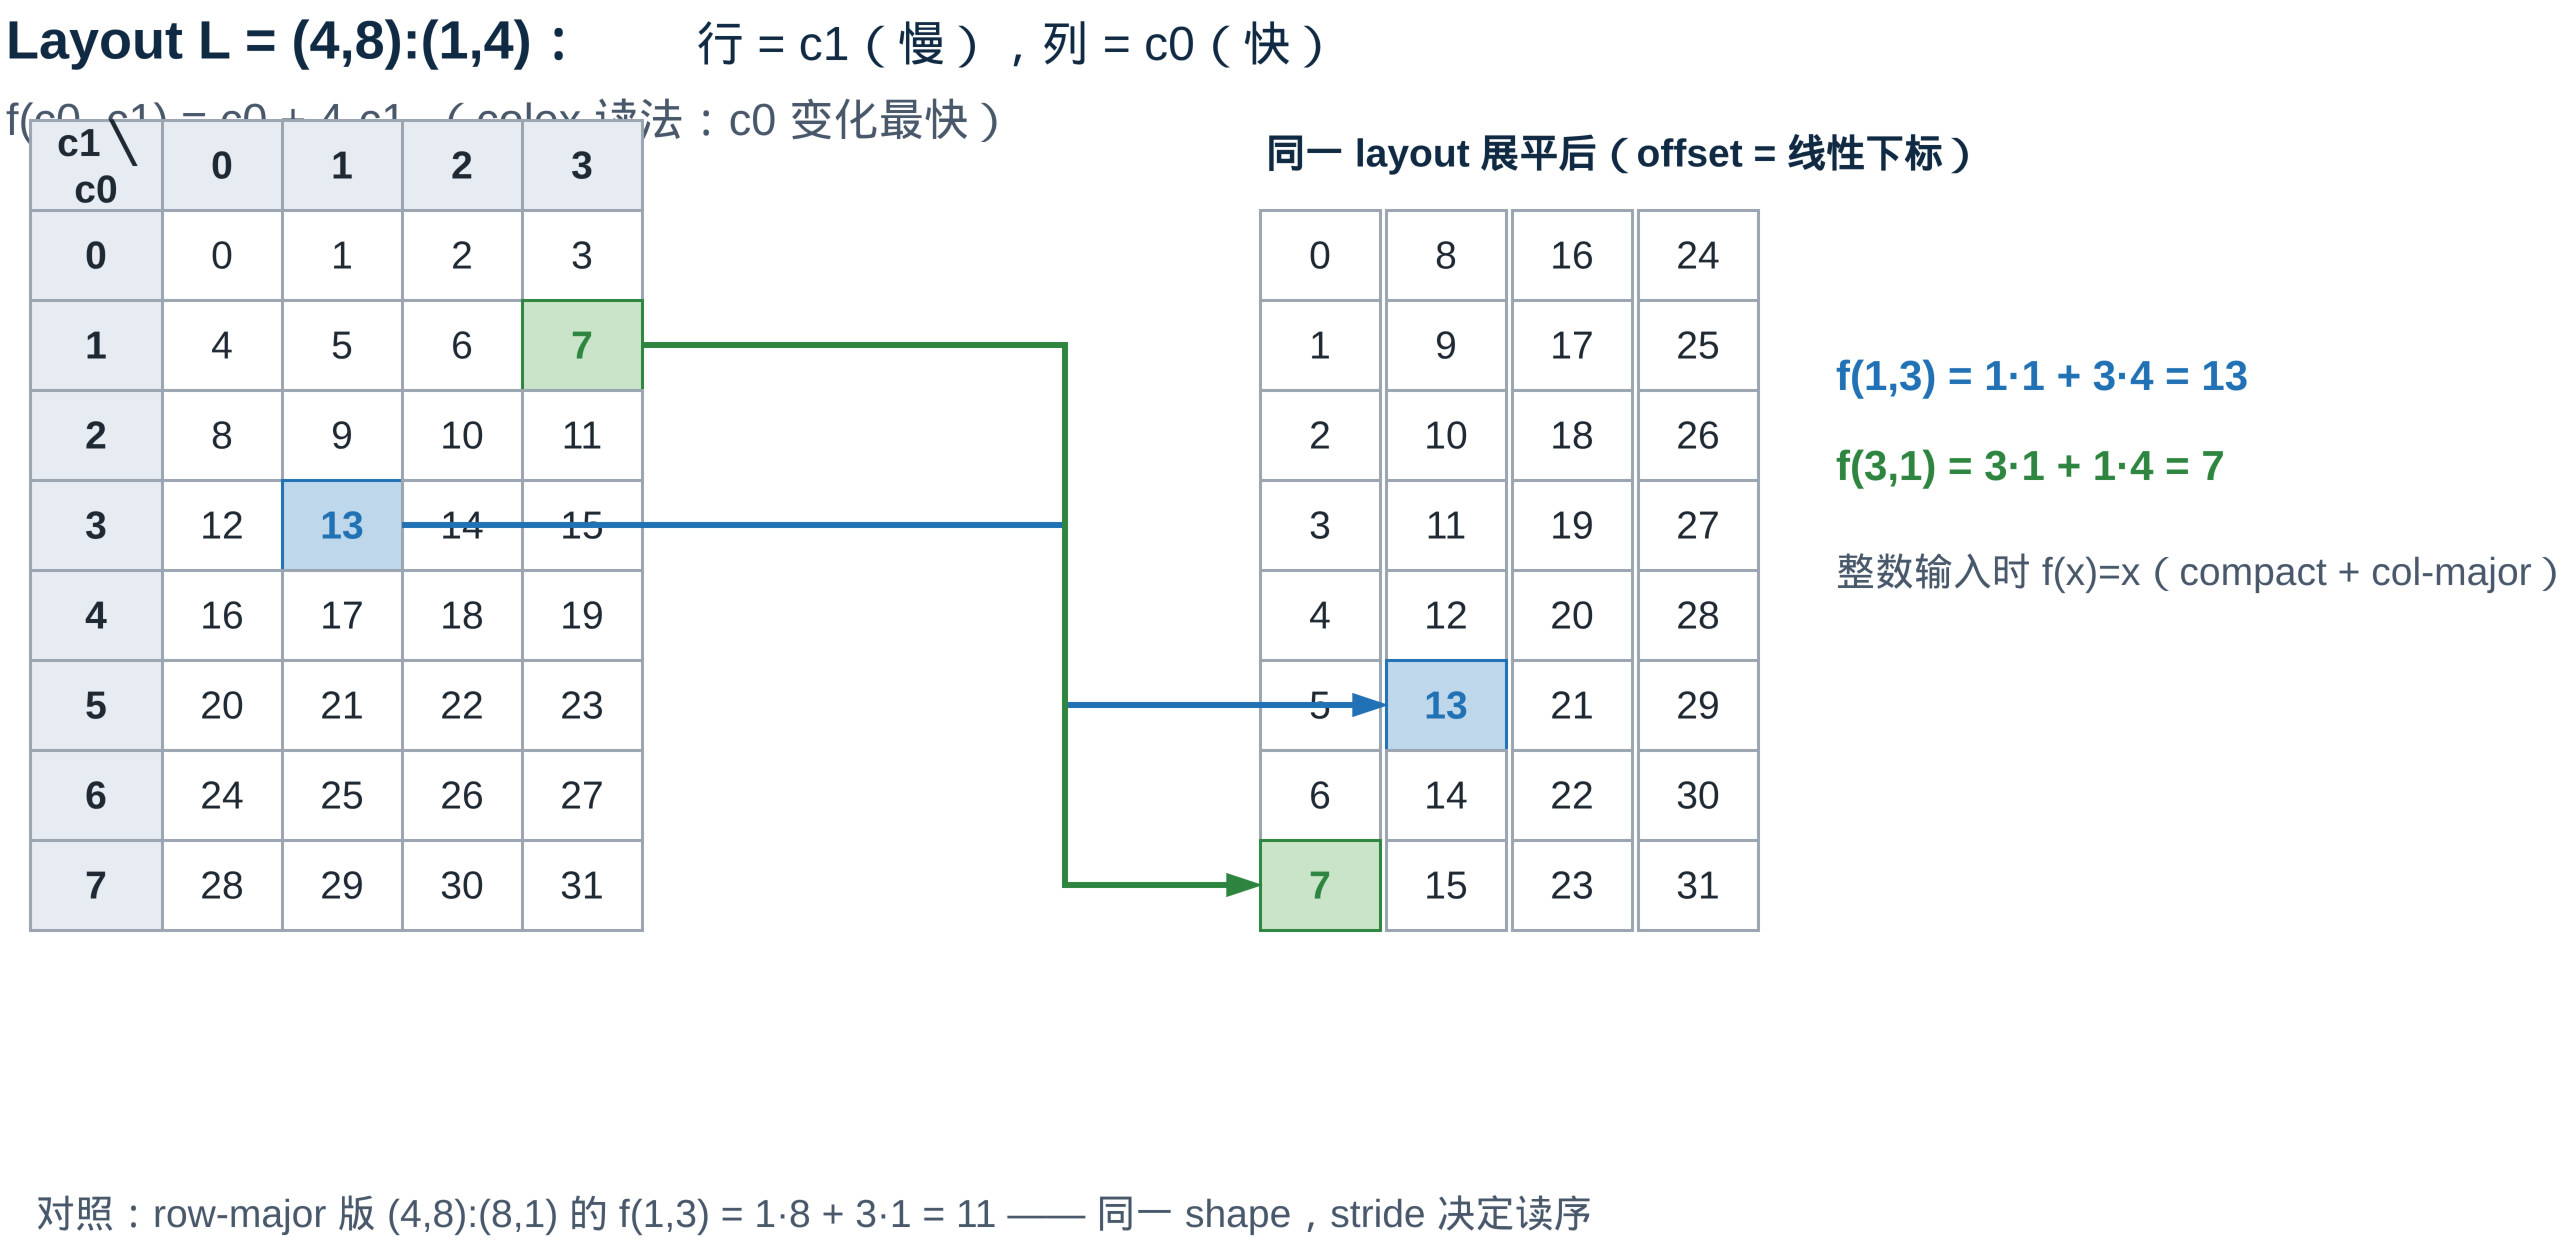
\includegraphics[width=0.92\textwidth]{figures/drawio/fig-20-1-colex/fig-20-1.png}
\begin{tikzpicture}[font=\footnotesize, x=1cm, y=1cm]
  % 单元格尺寸；表 = 行头列 + c0=0..3 列、列头行 + c1=0..7 行
  \def\cw{0.90}
  \def\chh{0.565}
  % 左：坐标表 f(c0,c1) = c0 + 4 c1
  \foreach \c in {0,...,5}{\draw[gray!45] (\c*\cw, 0) -- (\c*\cw, -9*\chh);}
  \foreach \r in {0,...,9}{\draw[gray!45] (0, -\r*\chh) -- (5*\cw, -\r*\chh);}
  \filldraw[fill=gray!22, draw=gray!55, thin] (0, -\chh) rectangle (\cw, -9*\chh);
  \filldraw[fill=gray!22, draw=gray!55, thin] (\cw, 0) rectangle (5*\cw, -\chh);
  \foreach \r/\rh in {0/1,1/2,2/3,3/4,4/5,5/6,6/7,7/8}{
    \edef\cfill{colorx\rh!16}
    \fill[\cfill] (\cw, {-(\r+1)*\chh}) rectangle (5*\cw, {-(\r+2)*\chh});
  }
  \node at (0.5*\cw, -0.5*\chh) {$c_1\backslash c_0$};
  \foreach \c in {0,1,2,3}{\node at ({(\c+1.5)*\cw}, -0.5*\chh) {\c};}
  \foreach \r in {0,...,7}{\node at (0.5*\cw, {-(\r+1.5)*\chh}) {\r};}
  \foreach \c in {0,1,2,3}{\foreach \r in {0,...,7}{%
    \pgfmathsetmacro\val{int(\c+4*\r)}%
    \node at ({(\c+1.5)*\cw}, {-(\r+1.5)*\chh}) {\val};}}
  % 高亮 f(1,3)=13（蓝）与 f(3,1)=7（绿）
  \fill[tkFillBlue] (2*\cw, -4*\chh) rectangle (3*\cw, -5*\chh);
  \draw[tkBlue, semithick] (2*\cw, -4*\chh) rectangle (3*\cw, -5*\chh);
  \node[text=tkBlue, font=\footnotesize\bfseries] at (2.5*\cw, -4.5*\chh) {13};
  \fill[tkFillGreen] (4*\cw, -2*\chh) rectangle (5*\cw, -3*\chh);
  \draw[tkGreen, semithick] (4*\cw, -2*\chh) rectangle (5*\cw, -3*\chh);
  \node[text=tkGreen, font=\footnotesize\bfseries] at (4.5*\cw, -2.5*\chh) {7};
  % 右：展平后的 1D 数带（列 j 自上而下为 8j..8j+7）
  \def\bx{6.83}
  \foreach \c in {0,...,4}{\draw[gray!45] ({\bx+\c*\cw}, -\chh) -- ({\bx+\c*\cw}, -9*\chh);}
  \foreach \r in {1,...,9}{\draw[gray!45] (\bx, -\r*\chh) -- ({\bx+4*\cw}, -\r*\chh);}
  \foreach \bg/\gt/\gb in {0/1/2,1/3/4,2/5/6,3/7/8}{
    \edef\cfillA{colorx\gt!16}
    \edef\cfillB{colorx\gb!16}
    \fill[\cfillA] ({\bx+\bg*\cw}, -\chh) rectangle ({\bx+(\bg+1)*\cw}, -5*\chh);
    \fill[\cfillB] ({\bx+\bg*\cw}, -5*\chh) rectangle ({\bx+(\bg+1)*\cw}, -9*\chh);
  }
  \foreach \c in {0,...,3}{\foreach \r in {0,...,7}{%
    \pgfmathsetmacro\val{int(8*\c+\r)}%
    \node at ({\bx+(\c+0.5)*\cw}, {-(\r+1.5)*\chh}) {\val};}}
  \fill[tkFillGreen] (\bx, -8*\chh) rectangle ({\bx+\cw}, -9*\chh);
  \draw[tkGreen, semithick] (\bx, -8*\chh) rectangle ({\bx+\cw}, -9*\chh);
  \node[text=tkGreen, font=\footnotesize\bfseries] at ({\bx+0.5*\cw}, -8.5*\chh) {7};
  \fill[tkFillBlue] ({\bx+\cw}, -6*\chh) rectangle ({\bx+2*\cw}, -7*\chh);
  \draw[tkBlue, semithick] ({\bx+\cw}, -6*\chh) rectangle ({\bx+2*\cw}, -7*\chh);
  \node[text=tkBlue, font=\footnotesize\bfseries] at ({\bx+1.5*\cw}, -6.5*\chh) {13};
  % 连线：绿沿表格右缘下行、经数带下方自 7 格底边进入；蓝沿数带行边界进入 13 格上边
  \draw[tkGreen, semithick, -{Stealth[length=4pt]}]
    (5*\cw, -2.5*\chh) -- (5*\cw, -9.75*\chh) -- ({\bx+0.5*\cw}, -9.75*\chh) -- ({\bx+0.5*\cw}, -9*\chh);
  \draw[tkBlue, semithick, -{Stealth[length=4pt]}]
    (5*\cw+0.12, -4.5*\chh) -- (5.55, -4.5*\chh) -- (5.55, -6*\chh) -- ({\bx+1.5*\cw}, -6*\chh);
  % 右侧注记与标题
  \node[anchor=west, text=tkBlue] at (10.75, -0.8) {$f(1,3) = 1\cdot 1 + 3\cdot 4 = 13$};
  \node[anchor=west, text=tkGreen] at (10.75, -1.3) {$f(3,1) = 3\cdot 1 + 1\cdot 4 = 7$};
  \node[anchor=west, text=black!55, font=\scriptsize] at (10.75, -1.85) {整数输入时 $f(x)=x$};
  \node[anchor=west, text=black!55, font=\scriptsize] at (10.75, -2.15) {（compact $+$ col-major）};
  \node[anchor=west] at (0, 0.95) {$\mathrm{Layout}\ \mathcal{L} = (4,8){:}(1,4)$：行 $= c_1$（慢），列 $= c_0$（快）};
  \node[anchor=west, text=black!60, font=\scriptsize] at (0, 0.5) {$f(c_0,c_1) = c_0 + 4\,c_1$（colex 读法：$c_0$ 变化最快）};
  \node[anchor=west] at (\bx, -0.12) {展平后 1D 数带（$\mathrm{offset} =$ 线性下标）};
  \node[anchor=west, text=black!60, font=\scriptsize] at (0, -6.3)
    {对照：row-major 版 $(4,8){:}(8,1)$ 的 $f(1,3) = 1\cdot 8 + 3\cdot 1 = 11$——同一 shape，stride 决定读序};
\end{tikzpicture}
\caption{colex 线性化：坐标 $(c_0,c_1)$ 与 offset 的对应表（左），同一
布局展平后的 1D 数带（右）。$c_0$ 沿行方向变化最快，故
$\mathrm{idx}=c_0+4c_1$；整数输入时 CuTe 用
式~\eqref{eq:20-colex-decomp} 先把 $x$ 分解回坐标。compact 且 col-major 时
$f(x)=x$。对照 row-major 版 $(4,8){:}(8,1)$：
$f(1,3)=11$——同一 shape，stride 决定读序。}
\label{fig:20-1}
\end{figure}

\begin{figure}[htbp]
\centering
% was: 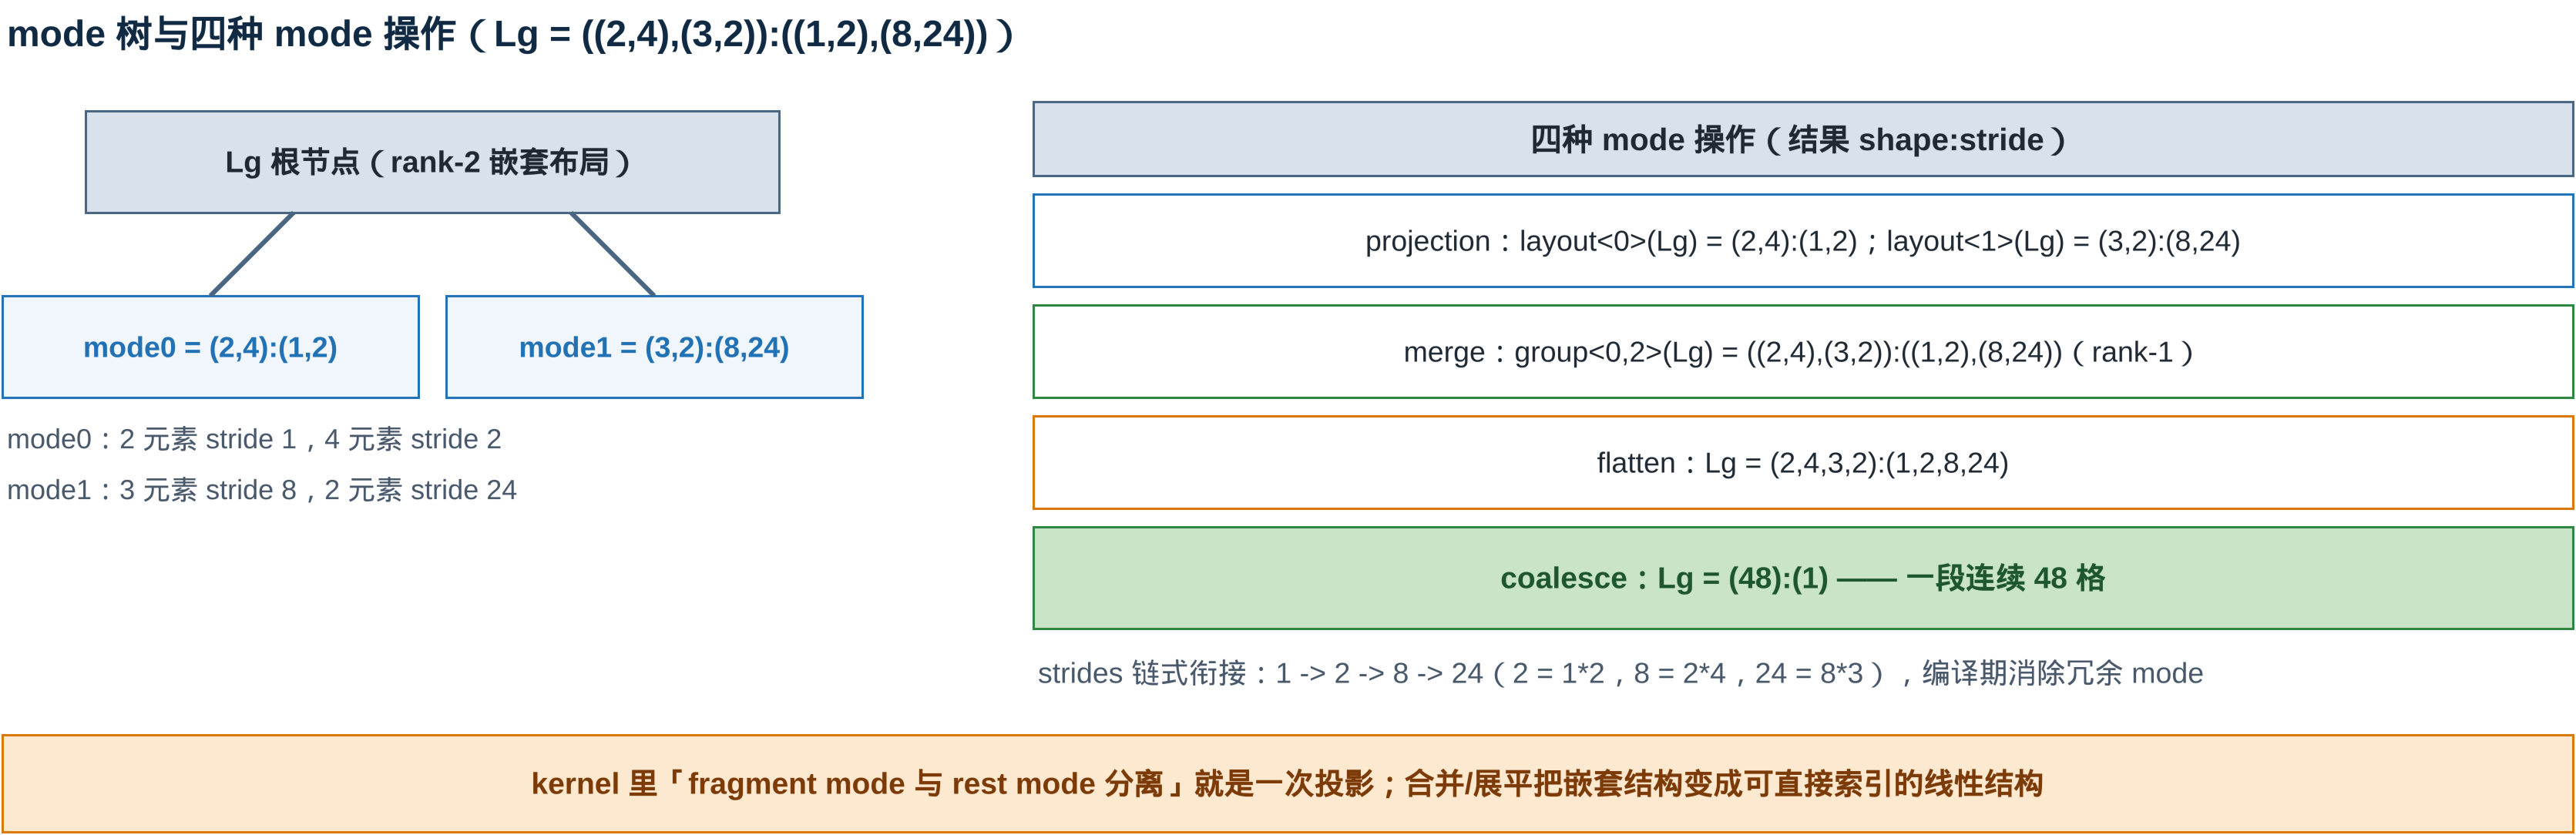
\includegraphics[width=0.95\textwidth]{figures/drawio/fig-20-2-mode-ops/fig-20-2.png}
\begin{tikzpicture}[font=\footnotesize, x=1cm, y=1cm,
    treenode/.style={draw=gray!60, fill=gray!12, align=center, inner sep=2pt, minimum height=0.66cm},
    modebox/.style={draw=tkBlue!75, fill=tkFillBlue, text=tkBlue, align=center, inner sep=2pt, minimum height=0.72cm},
    oprow/.style={draw, align=center, inner sep=2pt, minimum height=0.60cm, minimum width=10.4cm, anchor=west}]
  % 左：mode 树
  \node[treenode, minimum width=4.0cm] (root) at (2.30, -0.50) {$L_g$ 根节点（rank-2 嵌套布局）};
  \node[modebox, minimum width=2.1cm] (m0) at (1.15, -1.75) {mode0 $= (2,4){:}(1,2)$};
  \node[modebox, minimum width=2.1cm] (m1) at (3.45, -1.75) {mode1 $= (3,2){:}(8,24)$};
  \draw[gray!65] (2.30, -0.83) -- (2.30, -1.20);
  \draw[gray!65] (1.15, -1.20) -- (3.45, -1.20);
  \draw[gray!65] (1.15, -1.20) -- (1.15, -1.39);
  \draw[gray!65] (3.45, -1.20) -- (3.45, -1.39);
  \node[anchor=west, text=black!60, font=\scriptsize] at (0.0, -2.50) {mode0：2 元素 stride 1，4 元素 stride 2};
  \node[anchor=west, text=black!60, font=\scriptsize] at (0.0, -2.82) {mode1：3 元素 stride 8，2 元素 stride 24};
  % 右：四种 mode 操作
  \node[draw=gray!55, fill=gray!18, align=center, inner sep=2pt, minimum height=0.53cm, minimum width=10.4cm, anchor=west]
    at (6.60, -0.415) {四种 mode 操作（结果 shape$\,$:$\,$stride）};
  \node[oprow, draw=tkBlue!75] at (6.60, -0.98)
    {projection：$\mathrm{layout}\vert(L_g) = (2,4){:}(1,2)$；$\mathrm{layout}\vert(L_g) = (3,2){:}(8,24)$};
  \node[oprow, draw=tkGreen!75] at (6.60, -1.58)
    {merge：$\mathrm{group}\vert(L_g) = ((2,4),(3,2)){:}((1,2),(8,24))$（rank-1）};
  \node[oprow, draw=tkOrange!80] at (6.60, -2.18)
    {flatten：$L_g = (2,4,3,2){:}(1,2,8,24)$};
  \node[oprow, draw=tkGreen, fill=tkFillGreen, text=tkGreen!80!black, minimum height=0.66cm] at (6.60, -2.81)
    {coalesce：$L_g = (48){:}(1)$——一段连续 48 格};
  \node[anchor=west, text=black!60, font=\scriptsize] at (6.60, -3.55)
    {strides 链式衔接：$1 \to 2 \to 8 \to 24$（$2 = 1\times2$，$8 = 2\times4$，$24 = 8\times3$），编译期消除冗余 mode};
  % 底部结论条
  \node[draw=tkOrange!80, fill=tkFillOrange, text=tkOrange!75!black, align=center, inner sep=3pt,
    minimum height=0.70cm, minimum width=17.0cm] at (8.50, -4.45)
    {kernel 里\textbf{fragment mode 与 rest mode 分离}就是一次投影；合并/展平把嵌套结构变成可直接索引的线性结构};
  % 标题
  \node at (8.50, 0.55) {mode 树与四种 mode 操作（$L_g = ((2,4),(3,2)){:}((1,2),(8,24))$）};
\end{tikzpicture}
\caption{mode 树与四种 mode 操作的结果。投影用于取子布局，合并/展平用于把嵌套结构变成可直接索引的线性结构，化简（coalesce）在编译期消除冗余 mode——kernel 里\textbf{fragment mode 与 rest mode 分离}就是一次投影。}
\label{fig:20-2}
\end{figure}

\begin{figure}[htbp]
\centering
% was: 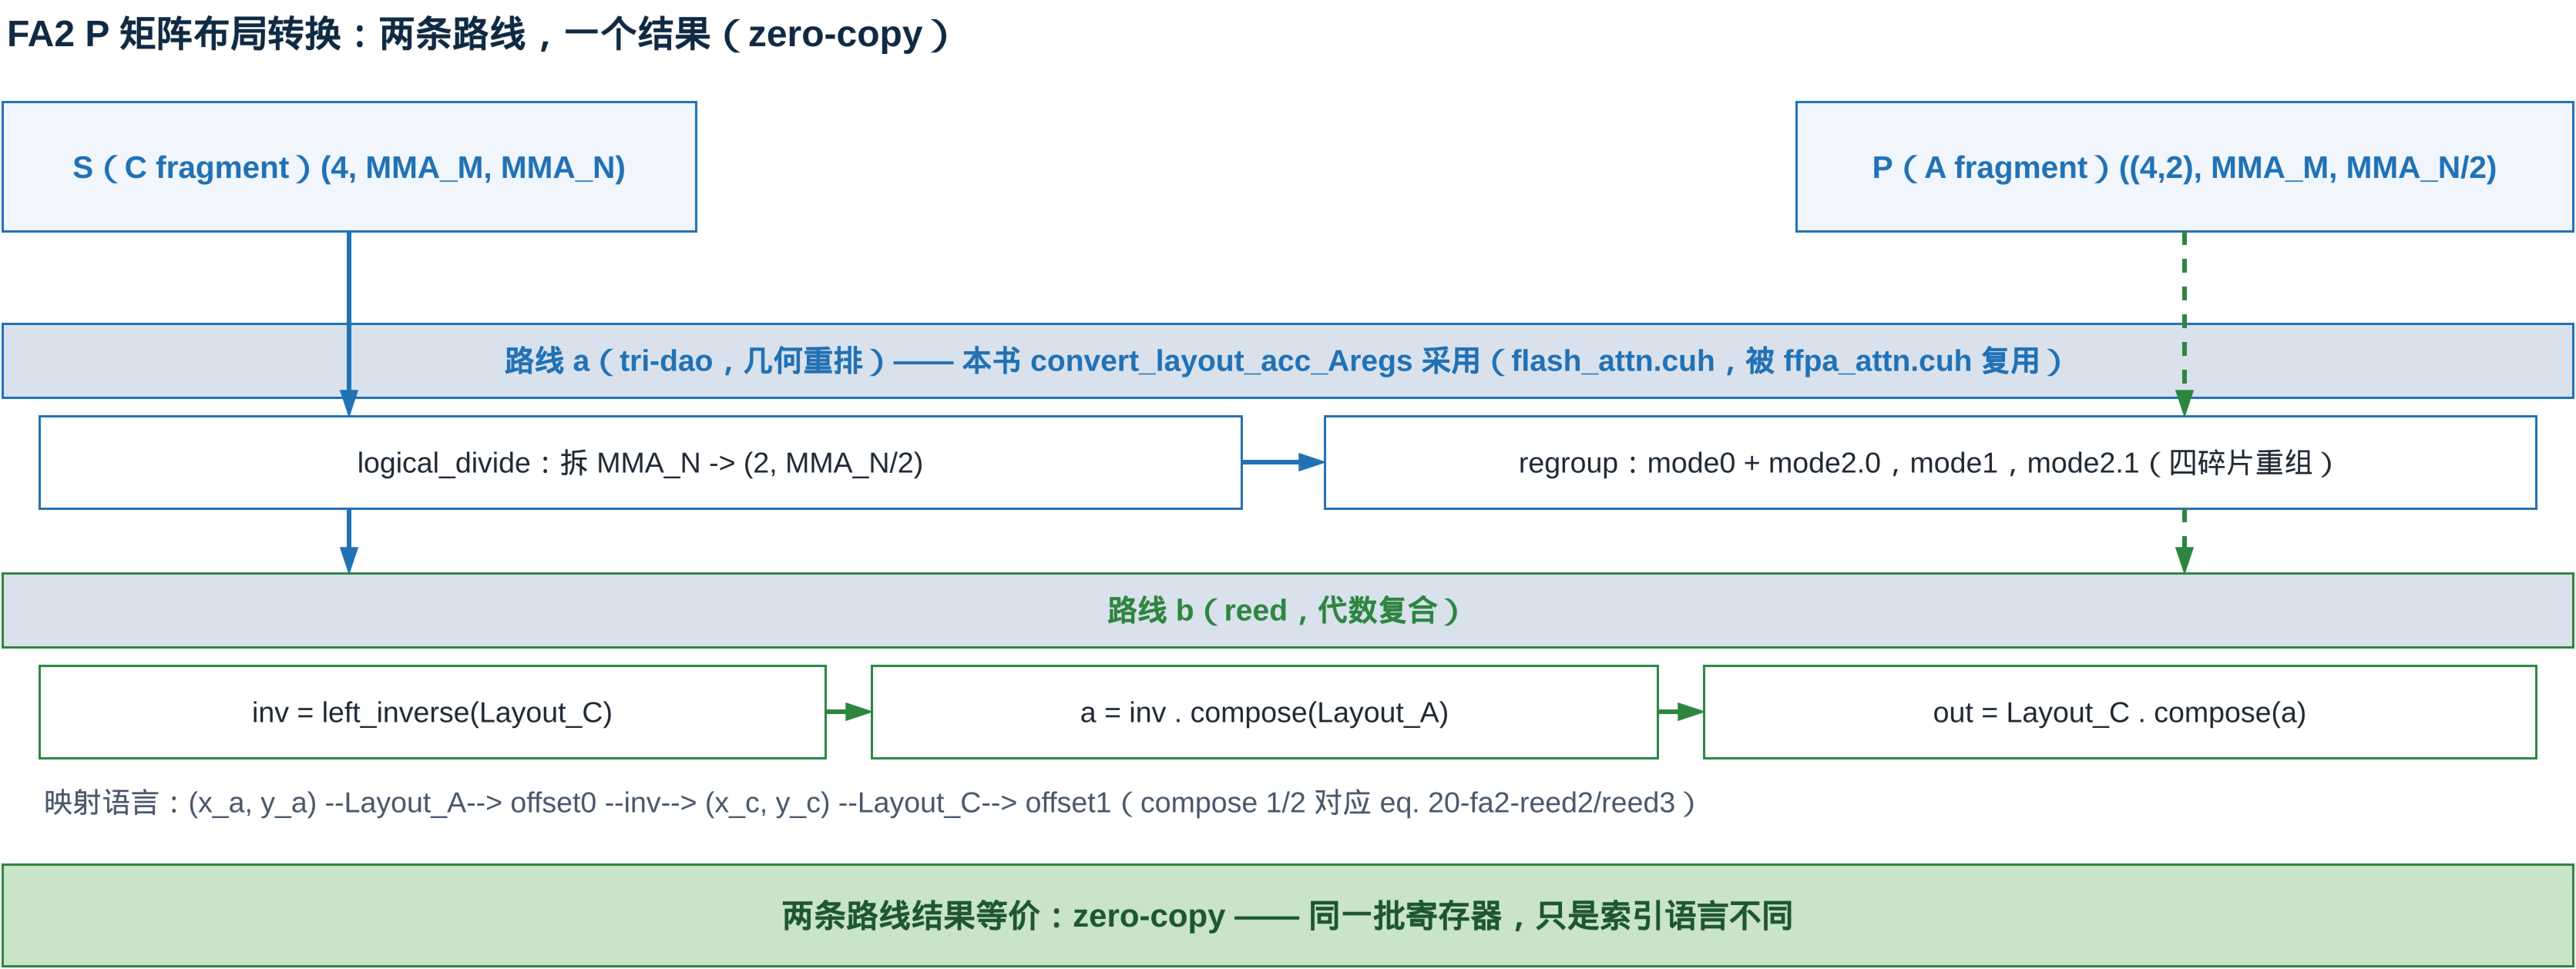
\includegraphics[width=0.95\textwidth]{figures/drawio/fig-20-3-layout-convert/fig-20-3.png}
\begin{tikzpicture}[font=\footnotesize, x=1cm, y=1cm,
    bluebox/.style={draw=tkBlue!75, fill=tkFillBlue, text=tkBlue!85!black, align=center, inner sep=2pt},
    stepbox/.style={draw=tkGreen!75, fill=white, text=black!85, align=center, inner sep=2pt},
    band/.style={draw, fill=gray!18, align=center, inner sep=2pt}]
  % 顶：源（C fragment）与目标（A fragment）
  \node[bluebox, minimum width=4.48cm, minimum height=0.83cm] at (2.24, -1.075)
    {S（C fragment）$(4,\ \mathrm{MMA\_M},\ \mathrm{MMA\_N})$};
  \node[bluebox, minimum width=5.02cm, minimum height=0.83cm] at (14.09, -1.075)
    {P（A fragment）$((4,2),\ \mathrm{MMA\_M},\ \mathrm{MMA\_N}/2)$};
  % 路线 a：几何重排（本书采用）
  \node[band, draw=tkBlue!75, text=tkBlue!85!black, font=\scriptsize, minimum width=16.60cm, minimum height=0.48cm]
    at (8.30, -2.33) {路线 a（tri-dao，几何重排）——本书 \texttt{convert\_layout\_acc\_Aregs} 采用（flash\_attn.cuh，被 ffpa\_attn.cuh 复用）};
  \node[draw=tkBlue!75, fill=white, align=center, inner sep=2pt, minimum width=7.76cm, minimum height=0.59cm]
    at (4.12, -2.985) {\texttt{logical\_divide}：拆 $\mathrm{MMA\_N} \to (2,\ \mathrm{MMA\_N}/2)$};
  \node[draw=tkBlue!75, fill=white, align=center, inner sep=2pt, minimum width=7.82cm, minimum height=0.59cm]
    at (12.45, -2.985) {\texttt{regroup}：mode0 $+$ mode2.0，mode1，mode2.1（四碎片重组）};
  % 路线 b：代数复合
  \node[band, draw=tkGreen!75, text=tkGreen!85!black, font=\scriptsize, minimum width=16.60cm, minimum height=0.48cm]
    at (8.30, -3.94) {路线 b（reed，代数复合）};
  \node[stepbox, minimum width=5.07cm, minimum height=0.60cm] at (2.775, -4.60)
    {\texttt{inv} $=$ \texttt{left\_inverse(Layout\_C)}};
  \node[stepbox, minimum width=5.08cm, minimum height=0.60cm] at (8.15, -4.60)
    {\texttt{a} $=$ \texttt{inv}\,$\cdot$\,\texttt{compose(Layout\_A)}};
  \node[stepbox, minimum width=5.37cm, minimum height=0.60cm] at (13.675, -4.60)
    {\texttt{out} $=$ \texttt{Layout\_C}\,$\cdot$\,\texttt{compose(a)}};
  \node[font=\scriptsize, text=black!60, anchor=center] at (8.30, -5.15)
    {映射语言：$(x_a, y_a)$ \texttt{--Layout\_A-->} offset0 \texttt{--inv-->} $(x_c, y_c)$ \texttt{--Layout\_C-->} offset1（compose 1/2 对应 \texttt{eq.\ 20-fa2-reed2/reed3}）};
  \node[draw=tkGreen, fill=tkFillGreen, text=tkGreen!80!black, align=center, inner sep=3pt,
    minimum width=16.60cm, minimum height=0.66cm] at (8.30, -5.91)
    {两条路线结果等价：Aregs 布局重解释是布局层 zero-copy；f32$\to$f16 另经 \texttt{convert\_type}};
  % 竖箭头：S -> 路线 a 首步；P -> regroup；两条路线各向下汇入
  \draw[tkBlue, semithick, -{Stealth[length=3.5pt]}] (2.24, -1.49) -- (2.24, -2.69);
  \draw[tkBlue, semithick, -{Stealth[length=3.5pt]}] (8.00, -2.985) -- (8.54, -2.985);
  \draw[tkBlue, semithick, -{Stealth[length=3.5pt]}] (2.24, -3.28) -- (2.24, -3.70);
  \draw[tkGreen, semithick, -{Stealth[length=3.5pt]}] (14.09, -1.49) -- (14.09, -2.69);
  \draw[tkGreen, semithick, -{Stealth[length=3.5pt]}] (14.09, -3.28) -- (14.09, -3.70);
  \draw[tkGreen, semithick, -{Stealth[length=3.5pt]}] (5.31, -4.60) -- (5.61, -4.60);
  \draw[tkGreen, semithick, -{Stealth[length=3.5pt]}] (10.69, -4.60) -- (10.99, -4.60);
  % 标题
  \node at (8.30, -0.21) {FA2 $P$ 矩阵布局转换：两条路线（布局层 zero-copy）};
\end{tikzpicture}
\caption{FA2 的 P 矩阵布局转换：tri-dao 的几何重排与 reed 的代数复合两条路线，布局层结果等价。图中 S 为 f32 累加器、P 为 f16 操作数时，P 的数值转换由 \texttt{convert\_type} 产生新 fragment，不属于 Aregs 的布局重解释；本书 flash\_attn.cuh 的 \texttt{convert\_\allowbreak{}layout\_\allowbreak{}acc\_\allowbreak{}Aregs}（被 ffpa\_attn.cuh 复用）采用的是几何路线。}
\label{fig:20-3}
\end{figure}

\begin{figure}[htbp]
\centering
% was: 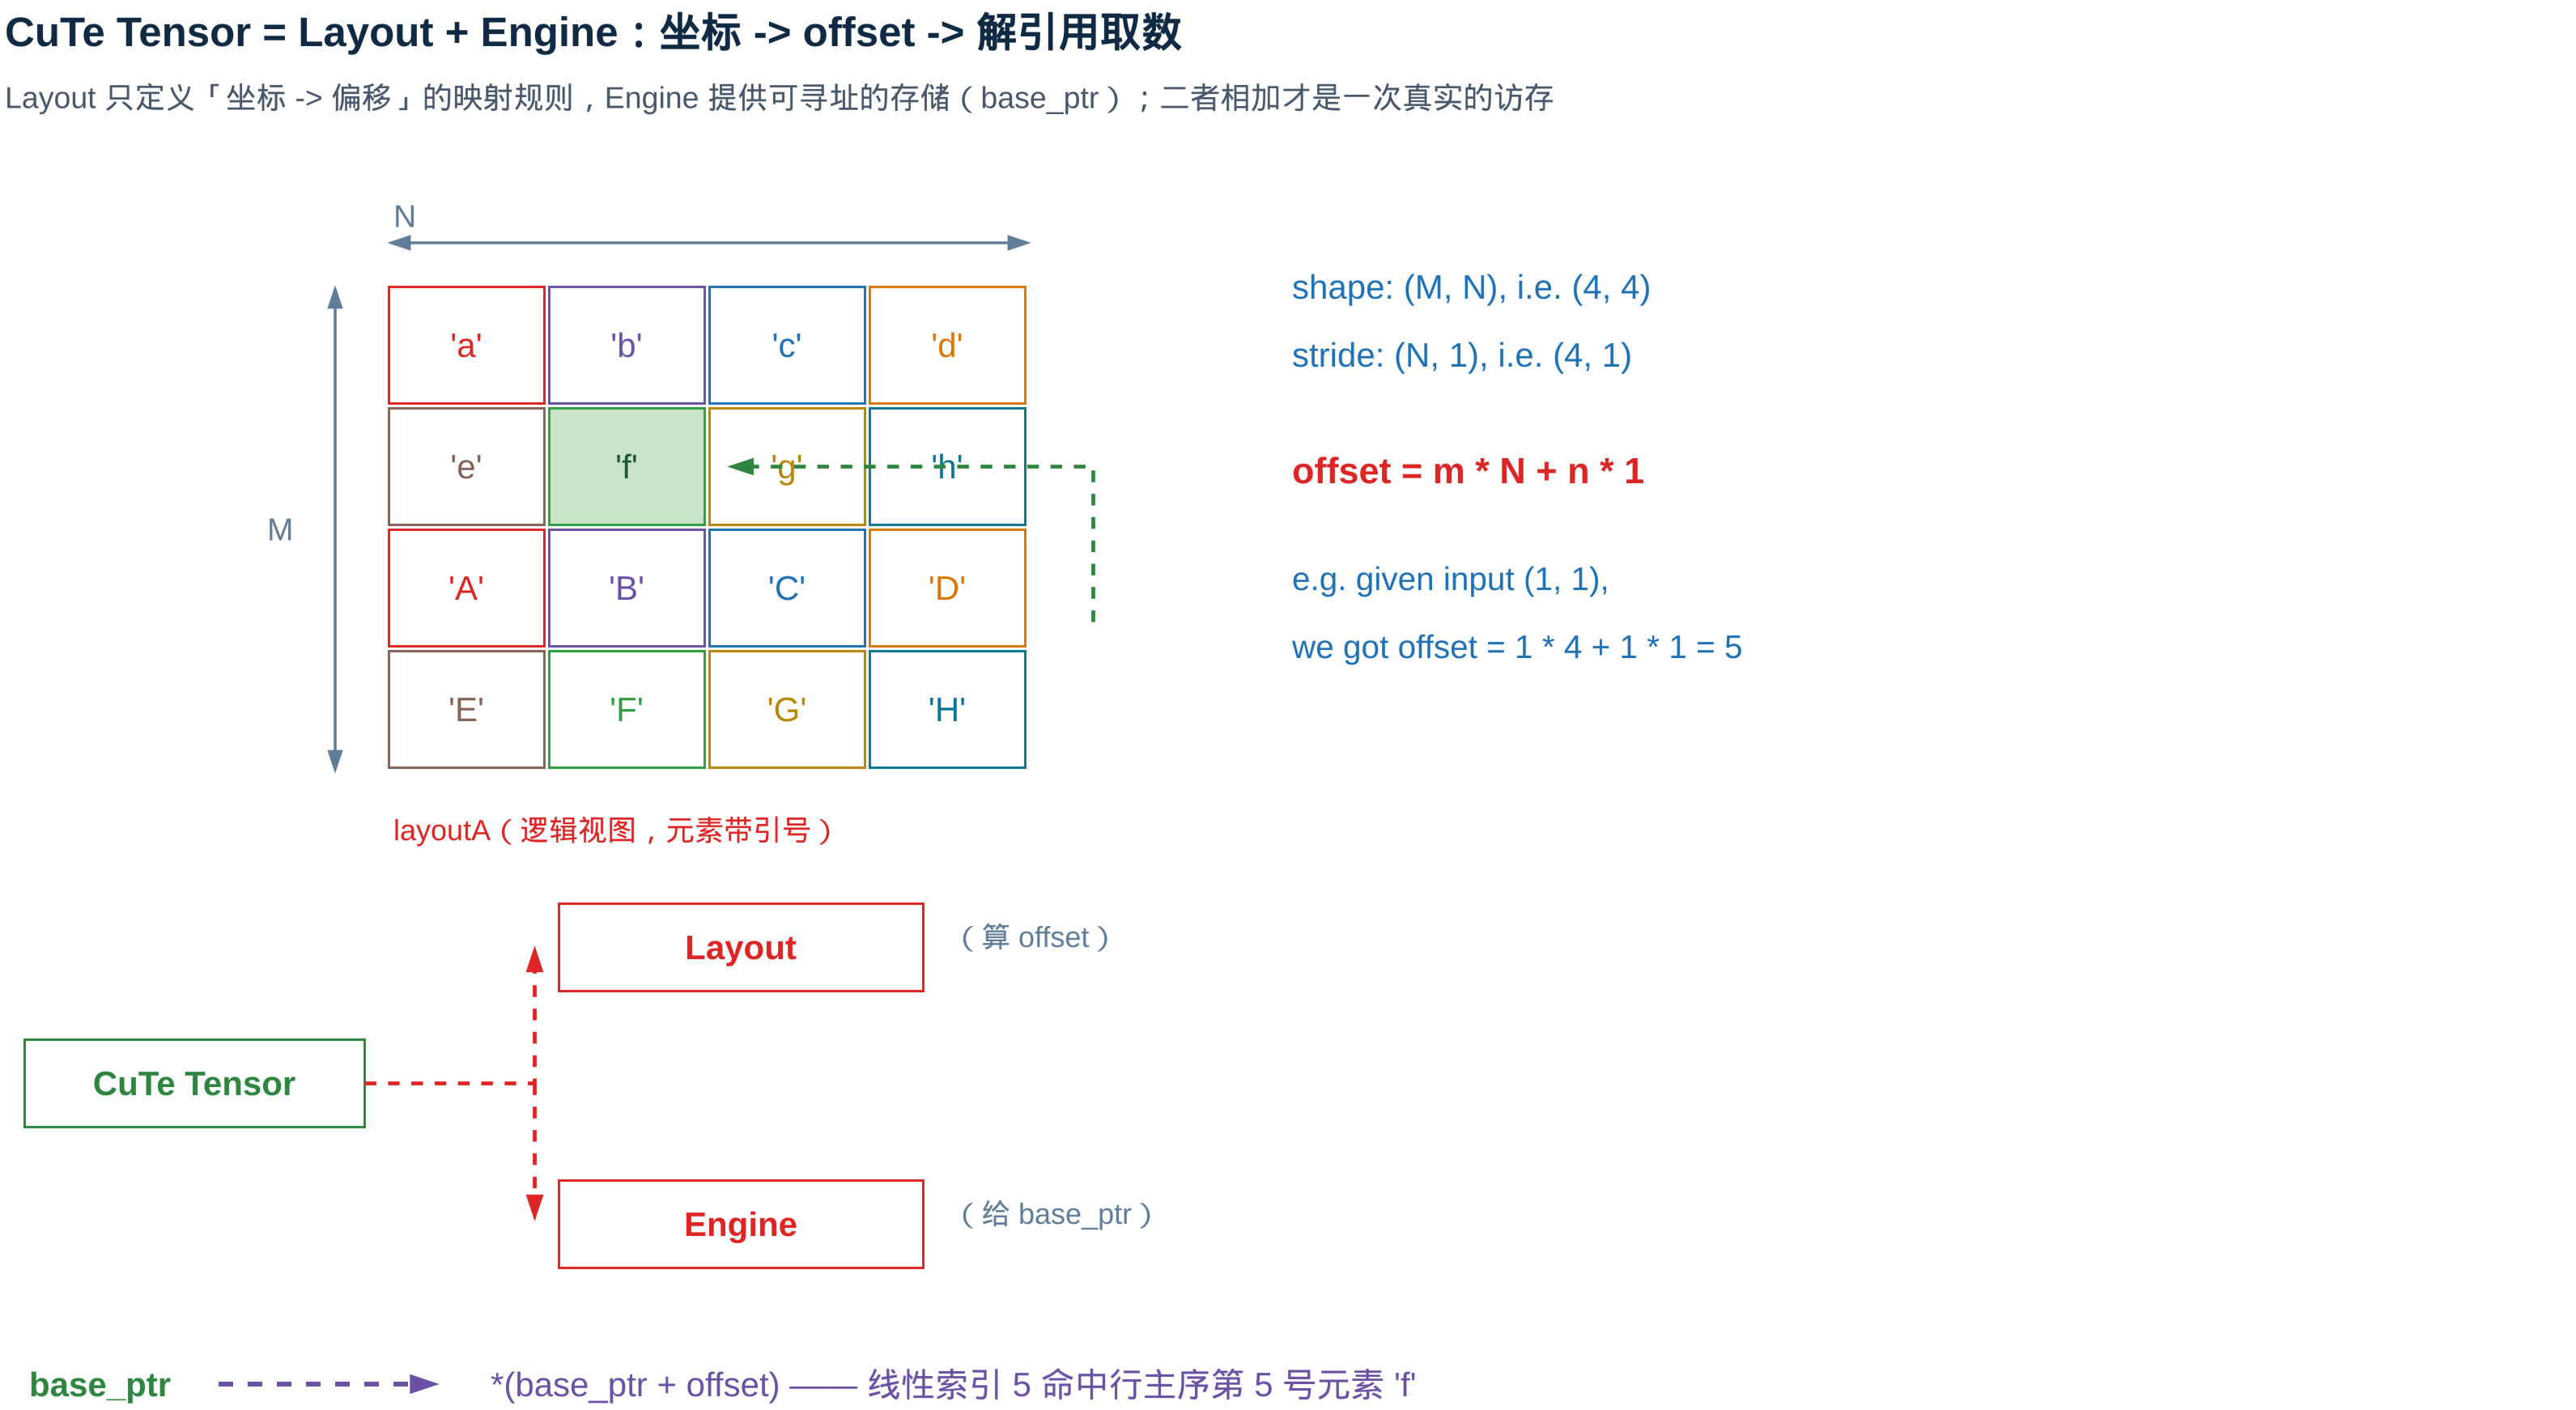
\includegraphics[width=0.95\textwidth]{figures/drawio/fig-20-4-tensor-addr/fig-20-4.png}
\begin{tikzpicture}[font=\footnotesize, x=1cm, y=1cm,
    cell/.style={draw=gray!45, fill=white, minimum width=0.985cm, minimum height=0.746cm, inner sep=0pt, font=\ttfamily},
    hitcell/.style={draw=tkGreen, fill=tkFillGreen, text=tkGreen!80!black, minimum width=0.985cm, minimum height=0.746cm, inner sep=0pt, font=\ttfamily},
    eqbox/.style={draw, fill=white, align=center, inner sep=2pt, minimum height=0.55cm}]
  % 4x4 元素网格（字符字面量，逻辑视图）
  \foreach \c/\ch in {0/a,1/b,2/c,3/d}{\node[cell] at ({2.9725+\c*0.985}, -2.133) {\texttt{'\ch'}};}
  \foreach \c/\ch in {0/e,1/f,2/g,3/h}{\node[cell] at ({2.9725+\c*0.985}, -2.879) {\texttt{'\ch'}};}
  \foreach \c/\ch in {0/A,1/B,2/C,3/D}{\node[cell] at ({2.9725+\c*0.985}, -3.625) {\texttt{'\ch'}};}
  \foreach \c/\ch in {0/E,1/F,2/G,3/H}{\node[cell] at ({2.9725+\c*0.985}, -4.371) {\texttt{'\ch'}};}
  \node[hitcell] at (3.9575, -2.879) {\texttt{'f'}};
  % 维度标注：N（列，上边）、M（行，左边）
  \draw[gray!70, {Stealth[length=2.5pt]}-{Stealth[length=2.5pt]}] (2.48, -1.49) -- (6.42, -1.49);
  \node[text=black!55] at (4.45, -1.33) {$N$};
  \draw[gray!70, {Stealth[length=2.5pt]}-{Stealth[length=2.5pt]}] (2.15, -1.76) -- (2.15, -4.74);
  \node[text=black!55] at (1.88, -3.25) {$M$};
  \node[anchor=west, text=tkRed, font=\scriptsize] at (2.48, -5.10) {layoutA（逻辑视图，元素带引号）};
  % 右侧：Layout 的代数定义与一次样例求值
  \node[anchor=west, text=tkBlue] at (8.00, -1.76) {shape: $(M, N)$, i.e. $(4, 4)$};
  \node[anchor=west, text=tkBlue] at (8.00, -2.18) {stride: $(N, 1)$, i.e. $(4, 1)$};
  \node[anchor=west, text=tkRed] at (8.00, -2.90) {offset $= m \times N + n \times 1$};
  \node[anchor=west, text=tkBlue] at (8.00, -3.55) {e.g. given input $(1, 1)$,};
  \node[anchor=west, text=tkBlue] at (8.00, -3.97) {we got offset $= 1 \times 4 + 1 \times 1 = 5$};
  \draw[tkGreen, semithick, -{Stealth[length=3.5pt]}] (6.80, -3.82) -- (4.42, -2.87);
  % 底部：Tensor = Layout + Engine
  \node[eqbox, draw=tkGreen, text=tkGreen!80!black, minimum width=2.09cm] at (1.285, -6.66) {CuTe Tensor};
  \node[eqbox, draw=tkRed, text=tkRed, minimum width=2.24cm] at (4.64, -5.82) {Layout};
  \node[eqbox, draw=tkRed, text=tkRed, minimum width=2.24cm] at (4.64, -7.52) {Engine};
  \node[anchor=west, text=black!55, font=\scriptsize] at (5.91, -5.76) {（算 offset）};
  \node[anchor=west, text=black!55, font=\scriptsize] at (5.91, -7.46) {（给 base\_ptr）};
  \draw[tkRed, dashed, -{Stealth[length=3pt]}] (2.33, -6.66) -- (3.37, -5.82);
  \draw[tkRed, dashed, -{Stealth[length=3pt]}] (3.37, -6.66) -- (3.37, -7.49);
  % 最底：解引用
  \node[anchor=west, text=tkGreen!80!black] at (0.24, -8.51) {base\_ptr};
  \draw[tkPurple, semithick, -{Stealth[length=3.5pt]}] (1.43, -8.51) -- (2.78, -8.51);
  \node[anchor=west, text=tkPurple] at (3.07, -8.51)
    {*(base\_ptr $+$ offset)——线性索引 5 命中行主序第 5 号元素 \texttt{'f'}};
  % 标题
  \node at (8.00, -0.19) {CuTe Tensor $=$ Layout $+$ Engine：坐标 $\to$ offset $\to$ 解引用取数};
  \node[text=black!60, font=\scriptsize] at (8.00, -0.60)
    {Layout 只定义\textbf{坐标 $\to$ 偏移}的映射规则，Engine 提供可寻址的存储（base\_ptr）；二者相加才是一次真实的访存};
\end{tikzpicture}
\caption{CuTe Tensor 的寻址分工：Layout 负责\textbf{坐标 $\to$ offset}的代数——shape 限定输入范围、stride 决定各 mode 步长；Engine 只持有 \texttt{base\_ptr}。$(1,1)\to 5$，命中行主序（$(4,4){:}(4,1)$，列连续）第 5 号元素 \texttt{f}。重建自 @竹熙佳处《写给大家看的 CuTe 教程：Layout Compose \& Inverse》。}
\label{fig:20-4}
\end{figure}

\begin{figure}[htbp]
\centering
% was: 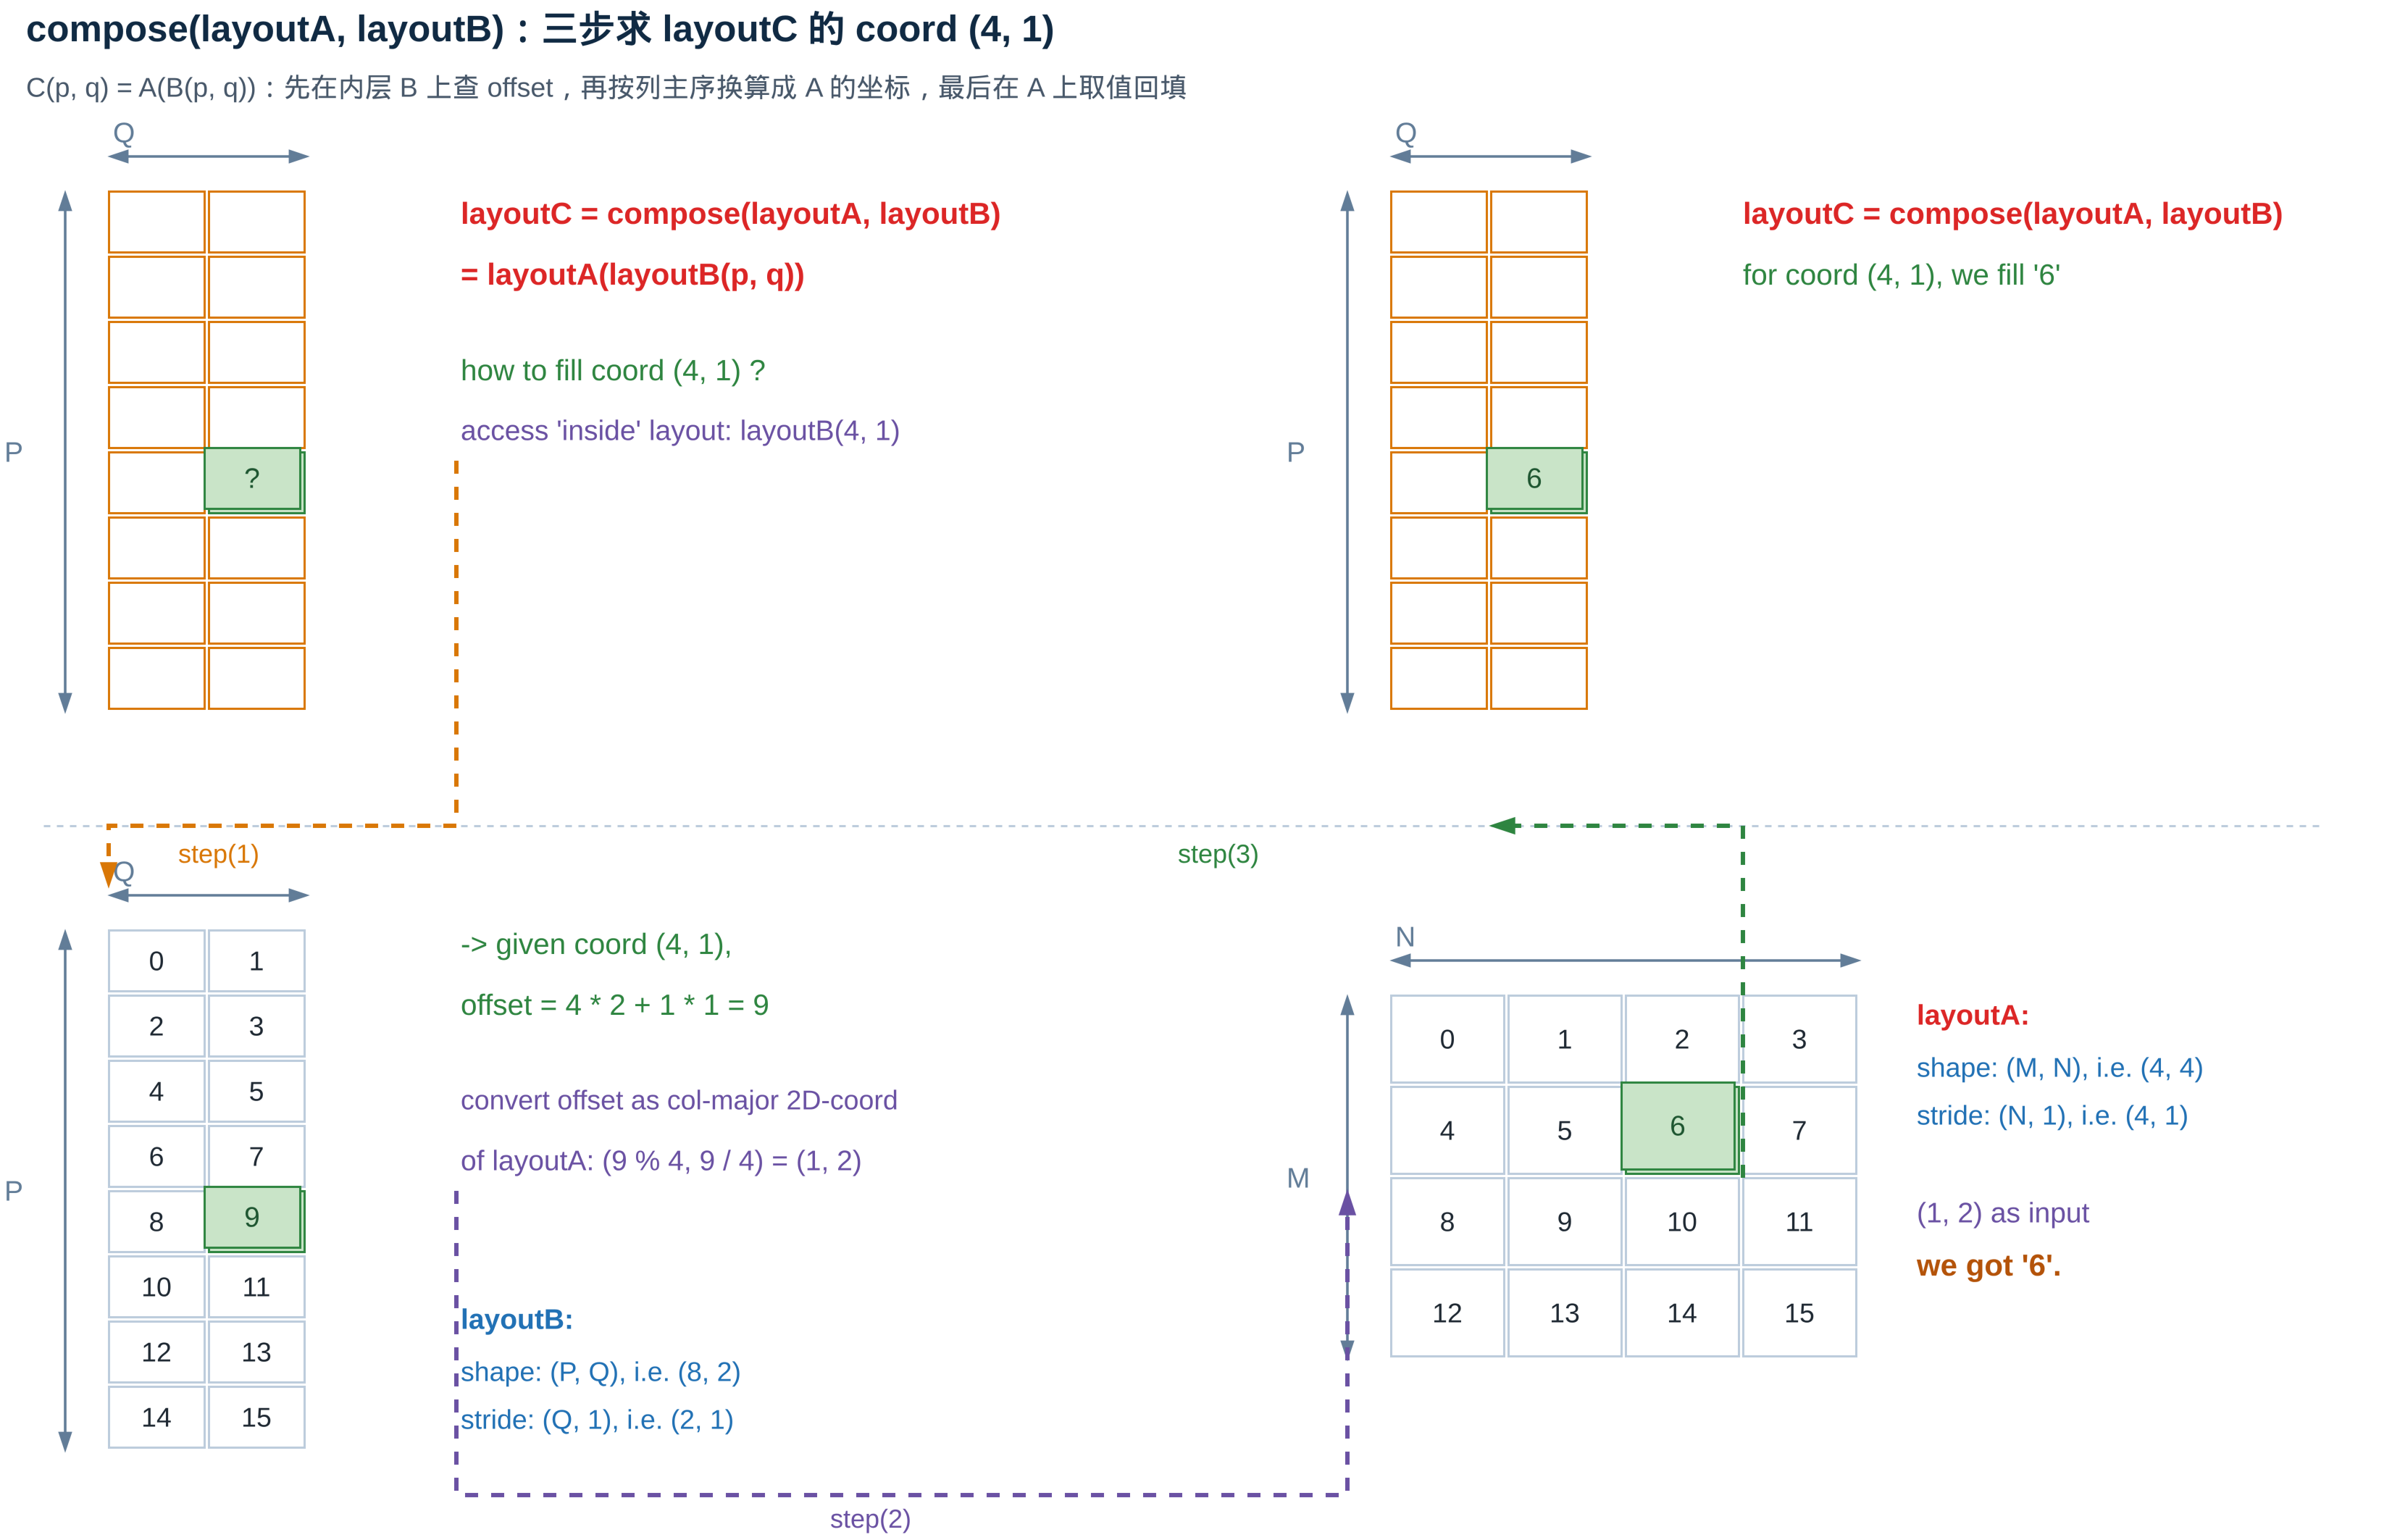
\includegraphics[width=0.95\textwidth]{figures/drawio/fig-20-5-compose-flow/fig-20-5.png}
\begin{tikzpicture}[font=\footnotesize, x=1cm, y=1cm,
    gcell/.style={draw=tkOrange!80, fill=white, minimum width=0.687cm, minimum height=0.448cm, inner sep=0pt},
    hcell/.style={draw=tkGreen, fill=tkFillGreen, text=tkGreen!80!black, minimum width=0.687cm, minimum height=0.448cm, inner sep=0pt},
    bgcell/.style={draw=gray!45, fill=white, minimum width=0.687cm, minimum height=0.448cm, inner sep=0pt},
    bhcell/.style={draw=tkGreen, fill=tkFillGreen, text=tkGreen!80!black, minimum width=0.687cm, minimum height=0.448cm, inner sep=0pt}]
  \def\gw{0.687}
  \def\gh{0.448}
  % 面板 1（step 1）：待填的 layoutC 网格，目标格未知
  \begin{scope}[shift={(0.687, -1.313)}]
    \foreach \c in {0,1}{\foreach \r in {0,...,7}{\draw[tkOrange!80, fill=white] (\c*\gw, -\r*\gh) rectangle ({\c*\gw+\gw}, {-\r*\gh-\gh});}}
    \fill[tkFillGreen] (\gw, -4*\gh) rectangle (2*\gw, -5*\gh);
    \draw[tkGreen, semithick] (\gw, -4*\gh) rectangle (2*\gw, -5*\gh);
    \node[text=tkGreen] at (1.5*\gw, -4.5*\gh) {?};
    \draw[gray!70, {Stealth[length=2.5pt]}-{Stealth[length=2.5pt]}] (0, 0.238) -- (2*\gw, 0.238);
    \node[text=black!55, font=\scriptsize] at (\gw, 0.40) {$Q$};
    \draw[gray!70, {Stealth[length=2.5pt]}-{Stealth[length=2.5pt]}] (-0.30, 0) -- (-0.30, -8*\gh);
    \node[text=black!55, font=\scriptsize] at (-0.57, -4*\gh) {$P$};
  \end{scope}
  % 面板 2（step 3 的结果）：目标格已填 6
  \begin{scope}[shift={(9.49, -1.313)}]
    \foreach \c in {0,1}{\foreach \r in {0,...,7}{\draw[tkOrange!80, fill=white] (\c*\gw, -\r*\gh) rectangle ({\c*\gw+\gw}, {-\r*\gh-\gh});}}
    \fill[tkFillGreen] (\gw, -4*\gh) rectangle (2*\gw, -5*\gh);
    \draw[tkGreen, semithick] (\gw, -4*\gh) rectangle (2*\gw, -5*\gh);
    \node[text=tkGreen!80!black] at (1.5*\gw, -4.5*\gh) {6};
    \draw[gray!70, {Stealth[length=2.5pt]}-{Stealth[length=2.5pt]}] (0, 0.238) -- (2*\gw, 0.238);
    \node[text=black!55, font=\scriptsize] at (\gw, 0.40) {$Q$};
    \draw[gray!70, {Stealth[length=2.5pt]}-{Stealth[length=2.5pt]}] (-0.30, 0) -- (-0.30, -8*\gh);
    \node[text=black!55, font=\scriptsize] at (-0.57, -4*\gh) {$P$};
  \end{scope}
  % 左下（step 2）：layoutB 的 8x2 元素带，查出 offset 9
  \begin{scope}[shift={(0.687, -6.39)}]
    \foreach \c in {0,1}{\foreach \r in {0,...,7}{%
      \pgfmathsetmacro\val{int(2*\r+\c)}%
      \draw[gray!45, fill=white] (\c*\gw, -\r*\gh) rectangle ({\c*\gw+\gw}, {-\r*\gh-\gh});
      \node at ({\c*\gw+0.5*\gw}, {-\r*\gh-0.5*\gh}) {\val};}}
    \fill[tkFillGreen] (\gw, -4*\gh) rectangle (2*\gw, -5*\gh);
    \draw[tkGreen, semithick] (\gw, -4*\gh) rectangle (2*\gw, -5*\gh);
    \node[text=tkGreen!80!black] at (1.5*\gw, -4.5*\gh) {9};
    \draw[gray!70, {Stealth[length=2.5pt]}-{Stealth[length=2.5pt]}] (0, 0.238) -- (2*\gw, 0.238);
    \node[text=black!55, font=\scriptsize] at (\gw, 0.40) {$Q$};
    \draw[gray!70, {Stealth[length=2.5pt]}-{Stealth[length=2.5pt]}] (-0.30, 0) -- (-0.30, -8*\gh);
    \node[text=black!55, font=\scriptsize] at (-0.57, -4*\gh) {$P$};
  \end{scope}
  % 右下（step 3）：layoutA 的 4x4 网格，按坐标 (1,2) 取值 6
  \begin{scope}[shift={(9.49, -6.84)}]
    \foreach \c in {0,...,3}{\foreach \r in {0,...,3}{%
      \pgfmathsetmacro\val{int(4*\r+\c)}%
      \draw[gray!45, fill=white] ({\c*0.806}, {-\r*0.627}) rectangle ({\c*0.806+0.806}, {-\r*0.627-0.627});
      \node at ({\c*0.806+0.403}, {-\r*0.627-0.3135}) {\val};}}
    \fill[tkFillGreen] ({2*0.806}, -0.627) rectangle ({3*0.806}, -2*0.627);
    \draw[tkGreen, semithick] ({2*0.806}, -0.627) rectangle ({3*0.806}, -2*0.627);
    \node[text=tkGreen!80!black] at ({2.5*0.806}, {-1.5*0.627}) {6};
    \draw[gray!70, {Stealth[length=2.5pt]}-{Stealth[length=2.5pt]}] (0, 0.238) -- ({4*0.806}, 0.238);
    \node[text=black!55, font=\scriptsize] at ({2*0.806}, 0.40) {$N$};
    \draw[gray!70, {Stealth[length=2.5pt]}-{Stealth[length=2.5pt]}] (-0.30, 0) -- (-0.30, {-4*0.627});
    \node[text=black!55, font=\scriptsize] at (-0.57, {-2*0.627}) {$M$};
  \end{scope}
  % 文字说明
  \node[anchor=west, text=tkRed] at (3.07, -1.46) {layoutC $=$ compose(layoutA, layoutB)};
  \node[anchor=west, text=tkRed] at (3.07, -1.88) {$=$ layoutA(layoutB(p, q))};
  \node[anchor=west, text=tkGreen] at (3.07, -2.54) {how to fill coord $(4, 1)$ ?};
  \node[anchor=west, text=tkPurple] at (3.07, -2.96) {access ``inside'' layout: layoutB$(4, 1)$};
  \node[anchor=west, text=tkRed] at (11.88, -1.46) {layoutC $=$ compose(layoutA, layoutB)};
  \node[anchor=west, text=tkGreen] at (11.88, -1.88) {for coord $(4, 1)$, we fill \texttt{'6'}};
  \node[anchor=west, text=tkGreen] at (3.07, -6.48) {$\to$ given coord $(4, 1)$,};
  \node[anchor=west, text=tkGreen] at (3.07, -6.90) {offset $= 4 \times 2 + 1 \times 1 = 9$};
  \node[anchor=west, text=tkPurple] at (3.07, -7.55) {convert offset as col-major 2D-coord};
  \node[anchor=west, text=tkPurple] at (3.07, -7.97) {of layoutA: $(9 \bmod 4,\ 9/4) = (1, 2)$};
  \node[anchor=west, text=tkBlue] at (3.07, -8.92) {layoutB:};
  \node[anchor=west, text=tkBlue] at (3.07, -9.28) {shape: $(P, Q)$, i.e. $(8, 2)$};
  \node[anchor=west, text=tkBlue] at (3.07, -9.61) {stride: $(Q, 1)$, i.e. $(2, 1)$};
  \node[anchor=west, text=tkRed] at (13.07, -6.84) {layoutA:};
  \node[anchor=west, text=tkBlue] at (13.07, -7.19) {shape: $(M, N)$, i.e. $(4, 4)$};
  \node[anchor=west, text=tkBlue] at (13.07, -7.52) {stride: $(N, 1)$, i.e. $(4, 1)$};
  \node[anchor=west, text=tkPurple] at (13.07, -8.18) {$(1, 2)$ as input};
  \node[anchor=west, text=tkOrange!90!black] at (13.07, -8.54) {we got \texttt{'6'}.};
  % 步骤标签（与虚线同色）
  \node[text=tkOrange!90!black, font=\scriptsize] at (2.03, -5.87) {step(1)};
  \node[text=tkGreen, font=\scriptsize] at (8.90, -5.87) {step(3)};
  \node[text=tkPurple, font=\scriptsize] at (6.51, -10.43) {step(2)};
  % 分隔线：上半为待填/结果，下半为三层求值细节
  \draw[gray!45, dashed] (0.24, -5.67) -- (15.91, -5.67);
  % 步骤箭头（折线绕行，避免穿越网格）
  \draw[tkOrange!90!black, semithick, dashed, -{Stealth[length=3.5pt]}]
    (3.07, -3.16) -- (2.35, -3.16) -- (2.35, -6.05) -- (0.687, -6.05) -- (0.687, -6.39);
  \draw[tkPurple, semithick, dashed, -{Stealth[length=3.5pt]}] (3.07, -8.18) -- (9.19, -8.18);
  \draw[tkGreen, semithick, dashed, -{Stealth[length=3.5pt]}]
    (11.91, -8.09) -- (12.85, -8.09) -- (12.85, -5.42) -- (10.40, -5.42);
  % 标题
  \node at (8.00, -0.19) {compose(layoutA, layoutB)：三步求 layoutC 的 coord $(4, 1)$};
  \node[text=black!60, font=\scriptsize] at (8.00, -0.60)
    {$C(p, q) = A(B(p, q))$：先在内层 $B$ 上查 offset，再按 $A$ 的 shape 作 colex 分解，最后在 $A$ 上取值回填};
\end{tikzpicture}
\caption{compose(A, B) 的三步求值：先查内层 B 得 offset，再按外层 A 的 shape 把 offset 换算回坐标，最后查 A 得最终值。例：$C(4,1)\to B(4,1)=9\to(9\bmod 4,\,9\div 4)=(1,2)\to A(1,2)=6$ 回填 $C$。重建自同上文。}
\label{fig:20-5}
\end{figure}

\begin{figure}[htbp]
\centering
% was: 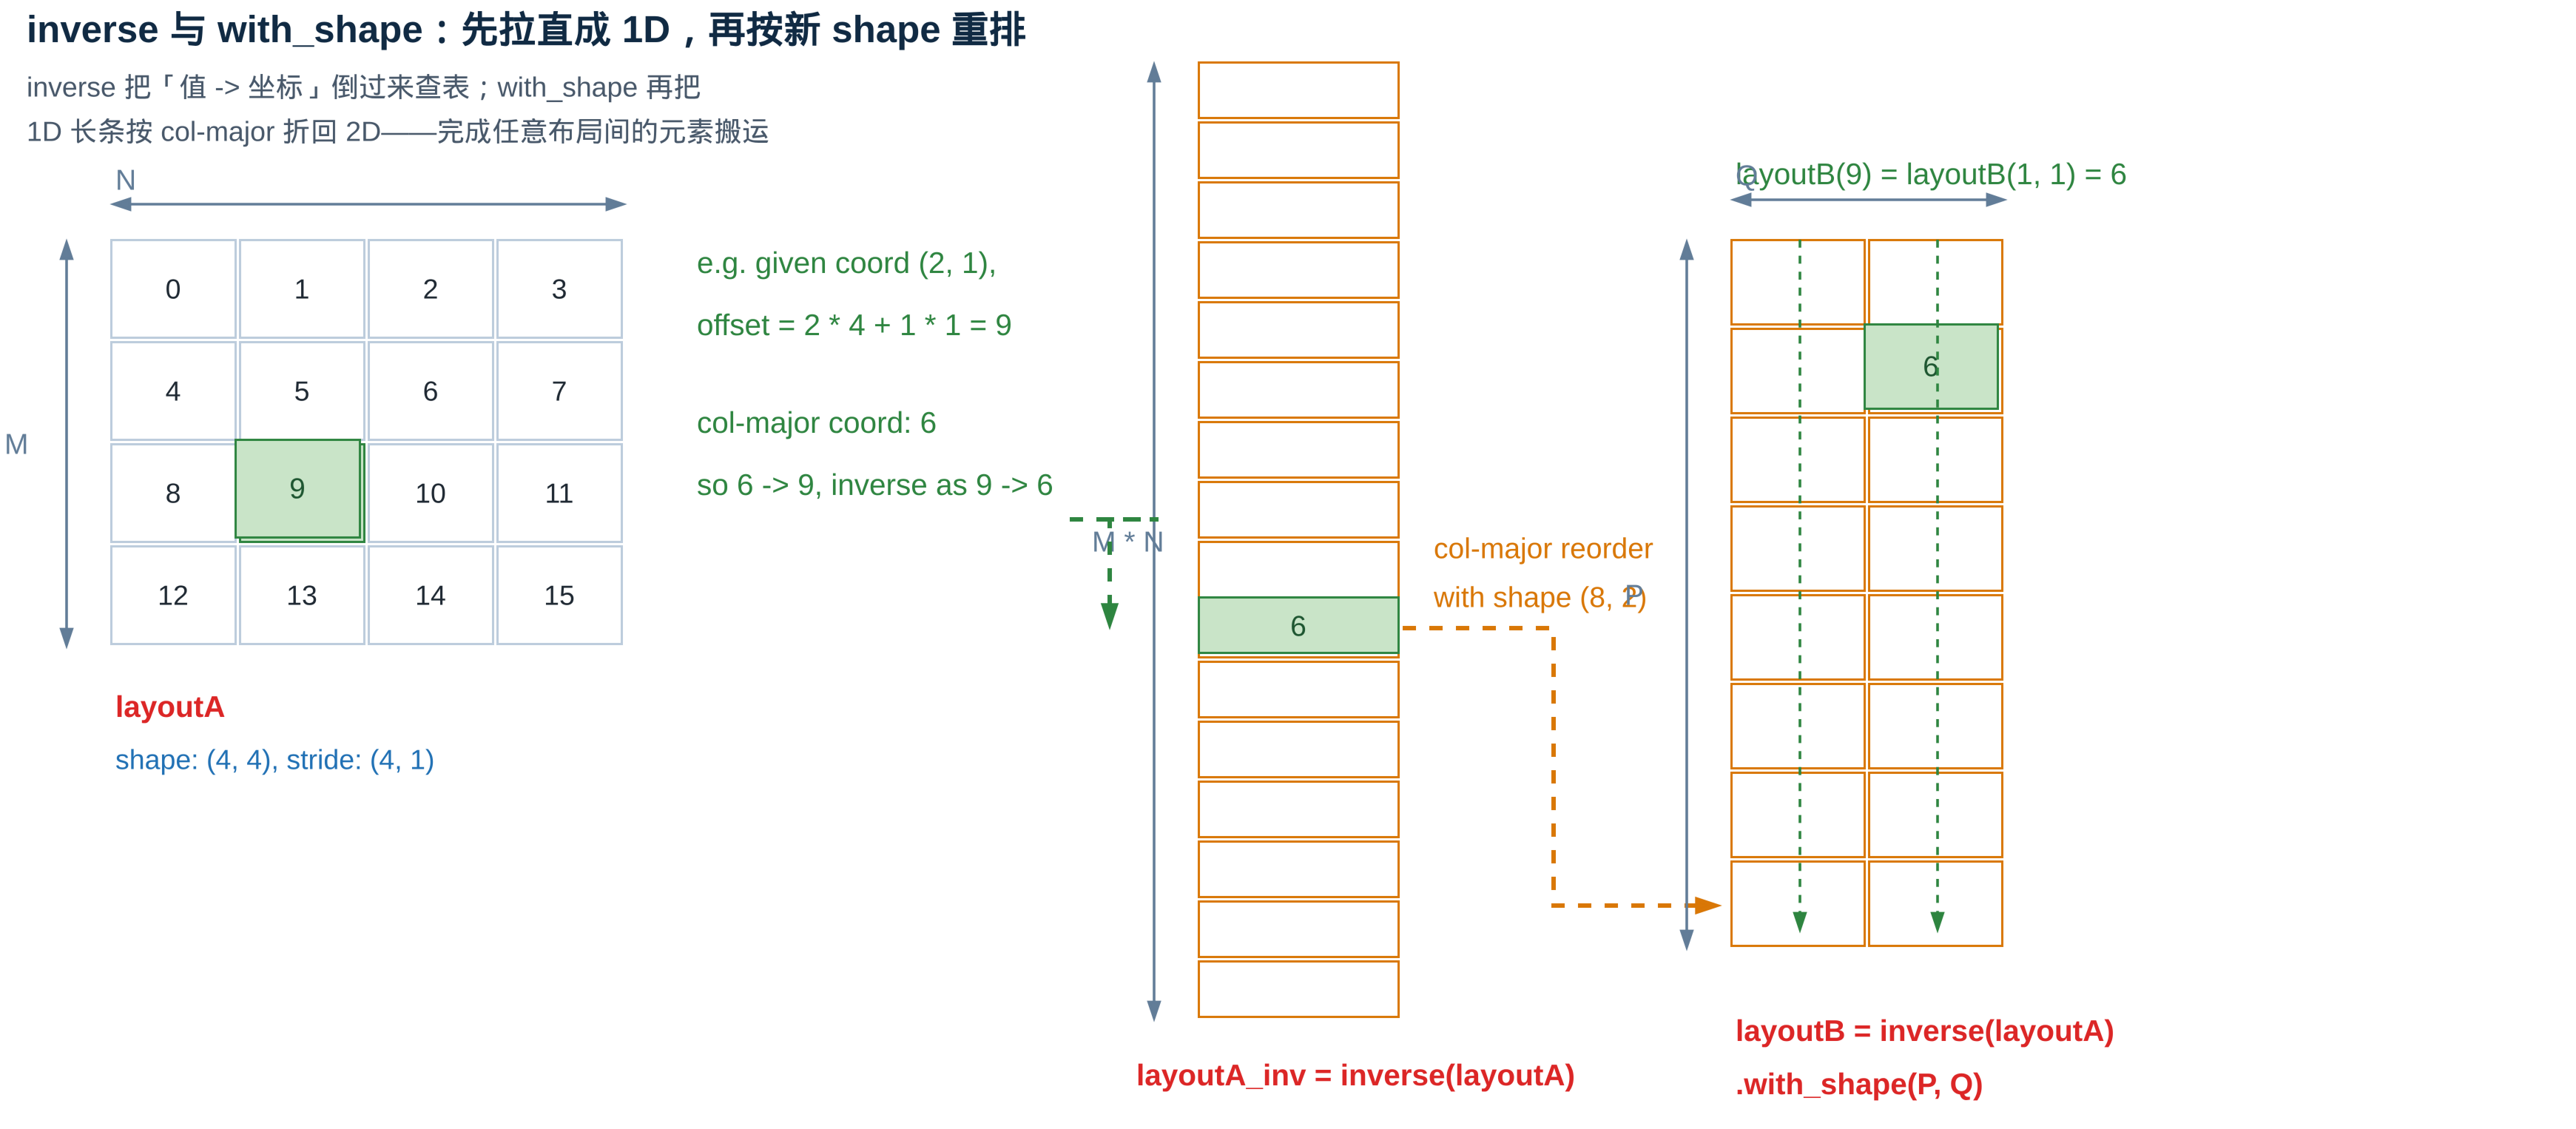
\includegraphics[width=0.95\textwidth]{figures/drawio/fig-20-6-inverse-reshape/fig-20-6.png}
\begin{tikzpicture}[font=\footnotesize, x=1cm, y=1cm]
  % 左：layoutA 的 4x4 矩阵（行主序）
  \begin{scope}[shift={(0.687, -1.612)}]
    \foreach \c in {0,...,3}{\foreach \r in {0,...,3}{%
      \pgfmathsetmacro\val{int(4*\r+\c)}%
      \draw[gray!45, fill=white] ({\c*0.866}, {-\r*0.687}) rectangle ({\c*0.866+0.866}, {-\r*0.687-0.687});
      \node at ({\c*0.866+0.433}, {-\r*0.687-0.3435}) {\val};}}
    \fill[tkFillGreen] (0.866, -2*0.687) rectangle (2*0.866, -3*0.687);
    \draw[tkGreen, semithick] (0.866, -2*0.687) rectangle (2*0.866, -3*0.687);
    \node[text=tkGreen!80!black] at (1.5*0.866, -2.5*0.687) {9};
    \draw[gray!70, {Stealth[length=2.5pt]}-{Stealth[length=2.5pt]}] (0, 0.239) -- ({4*0.866}, 0.239);
    \node[text=black!55, font=\scriptsize] at ({2*0.866}, 0.40) {$N$};
    \draw[gray!70, {Stealth[length=2.5pt]}-{Stealth[length=2.5pt]}] (-0.30, 0) -- (-0.30, {-4*0.687});
    \node[text=black!55, font=\scriptsize] at (-0.57, {-2*0.687}) {$M$};
  \end{scope}
  \node[anchor=west, text=tkRed] at (0.687, -4.60) {layoutA};
  \node[anchor=west, text=tkBlue] at (0.687, -4.96) {shape: $(4, 4)$, stride: $(4, 1)$};
  % 中：反查原始 offset
  \node[anchor=west, text=tkGreen] at (4.60, -1.76) {e.g. given coord $(2, 1)$,};
  \node[anchor=west, text=tkGreen] at (4.60, -2.18) {offset $= 2 \times 4 + 1 \times 1 = 9$};
  \node[anchor=west, text=tkGreen] at (4.60, -2.84) {col-major coord: 6};
  \node[anchor=west, text=tkGreen] at (4.60, -3.25) {so $6 \to 9$, inverse as $9 \to 6$};
  % 中：拉直成 1D 长条（16 格），第 9 格为 inverse 结果
  \begin{scope}[shift={(8.00, -0.418)}]
    \foreach \k in {0,...,15}{\draw[tkOrange!80, fill=white] (0, {-\k*0.403}) rectangle (1.343, {-\k*0.403-0.403});}
    \fill[tkFillGreen] (0, -8*0.403) rectangle (1.343, -9*0.403);
    \draw[tkGreen, semithick] (0, -8*0.403) rectangle (1.343, -9*0.403);
    \node[text=tkGreen!80!black] at (0.6715, -8.5*0.403) {6};
    \draw[gray!70, {Stealth[length=2.5pt]}-{Stealth[length=2.5pt]}] (-0.30, 0) -- (-0.30, {-16*0.403});
  \end{scope}
  \node[anchor=east, text=black!55, font=\scriptsize] at (7.65, -3.64) {$M \times N$};
  \node[anchor=west, text=tkOrange!90!black] at (9.55, -3.24) {col-major reorder};
  \node[anchor=west, text=tkOrange!90!black] at (9.55, -3.70) {with shape $(8, 2)$};
  % 右：按 col-major 折回 (P, Q) = (8, 2)
  \begin{scope}[shift={(11.58, -1.612)}]
    \foreach \c in {0,1}{\foreach \r in {0,...,7}{\draw[tkOrange!80, fill=white] ({\c*0.925}, {-\r*0.597}) rectangle ({\c*0.925+0.925}, {-\r*0.597-0.597});}}
    \fill[tkFillGreen] (0.925, 0) rectangle (2*0.925, -0.597);
    \draw[tkGreen, semithick] (0.925, 0) rectangle (2*0.925, -0.597);
    \node[text=tkGreen!80!black] at (1.5*0.925, -0.5*0.597) {6};
    \draw[tkGreen, dashed, -{Stealth[length=3pt]}] (0.25, -0.10) -- (0.25, {-8*0.597+0.30});
    \draw[tkGreen, dashed, -{Stealth[length=3pt]}] (1.62, -0.70) -- (1.62, {-8*0.597+0.30});
    \draw[gray!70, {Stealth[length=2.5pt]}-{Stealth[length=2.5pt]}] (0, 0.272) -- ({2*0.925}, 0.272);
    \node[text=black!55, font=\scriptsize] at (0.925, 0.43) {$Q$};
    \draw[gray!70, {Stealth[length=2.5pt]}-{Stealth[length=2.5pt]}] (-0.30, 0) -- (-0.30, {-8*0.597});
    \node[text=black!55, font=\scriptsize] at (-0.57, {-4*0.597}) {$P$};
  \end{scope}
  \node[anchor=west, text=tkGreen] at (11.58, -0.88) {layoutB$(9)$ $=$ layoutB$(1, 1)$ $=$ 6};
  \node[anchor=west, text=tkRed] at (11.58, -6.70) {layoutB $=$ inverse(layoutA)};
  \node[anchor=west, text=tkRed] at (11.58, -7.20) {.with\_shape$(P, Q)$};
  % 流程箭头
  \draw[tkGreen, dashed, -{Stealth[length=3pt]}] (7.13, -3.49) -- (7.40, -4.22);
  \draw[tkOrange!90!black, dashed, -{Stealth[length=3pt]}] (9.37, -4.22) -- (11.51, -6.09);
  % 标题
  \node at (8.00, -0.19) {inverse 与 with\_shape：先拉直成 1D，再按新 shape 重排};
  \node[anchor=west, text=black!60, font=\scriptsize] at (0.09, -0.58)
    {inverse 把\textbf{值 $\to$ 坐标}倒过来查表；with\_shape 再把};
  \node[anchor=west, text=black!60, font=\scriptsize] at (0.09, -0.86)
    {1D 长条按 col-major 折回 2D——完成任意布局间的元素搬运};
\end{tikzpicture}
\caption{inverse 与 with\_shape：inverse 把\textbf{值 $\to$ 坐标}倒过来查表（$9\leftrightarrow 6$ 互逆），with\_shape 再把 1D 长条按新 shape $(8,2)$ 沿 col-major 折回 2D，得 $B(1,1)=6$。重建自同上文。}
\label{fig:20-6}
\end{figure}

\begin{figure}[htbp]
\centering
% was: 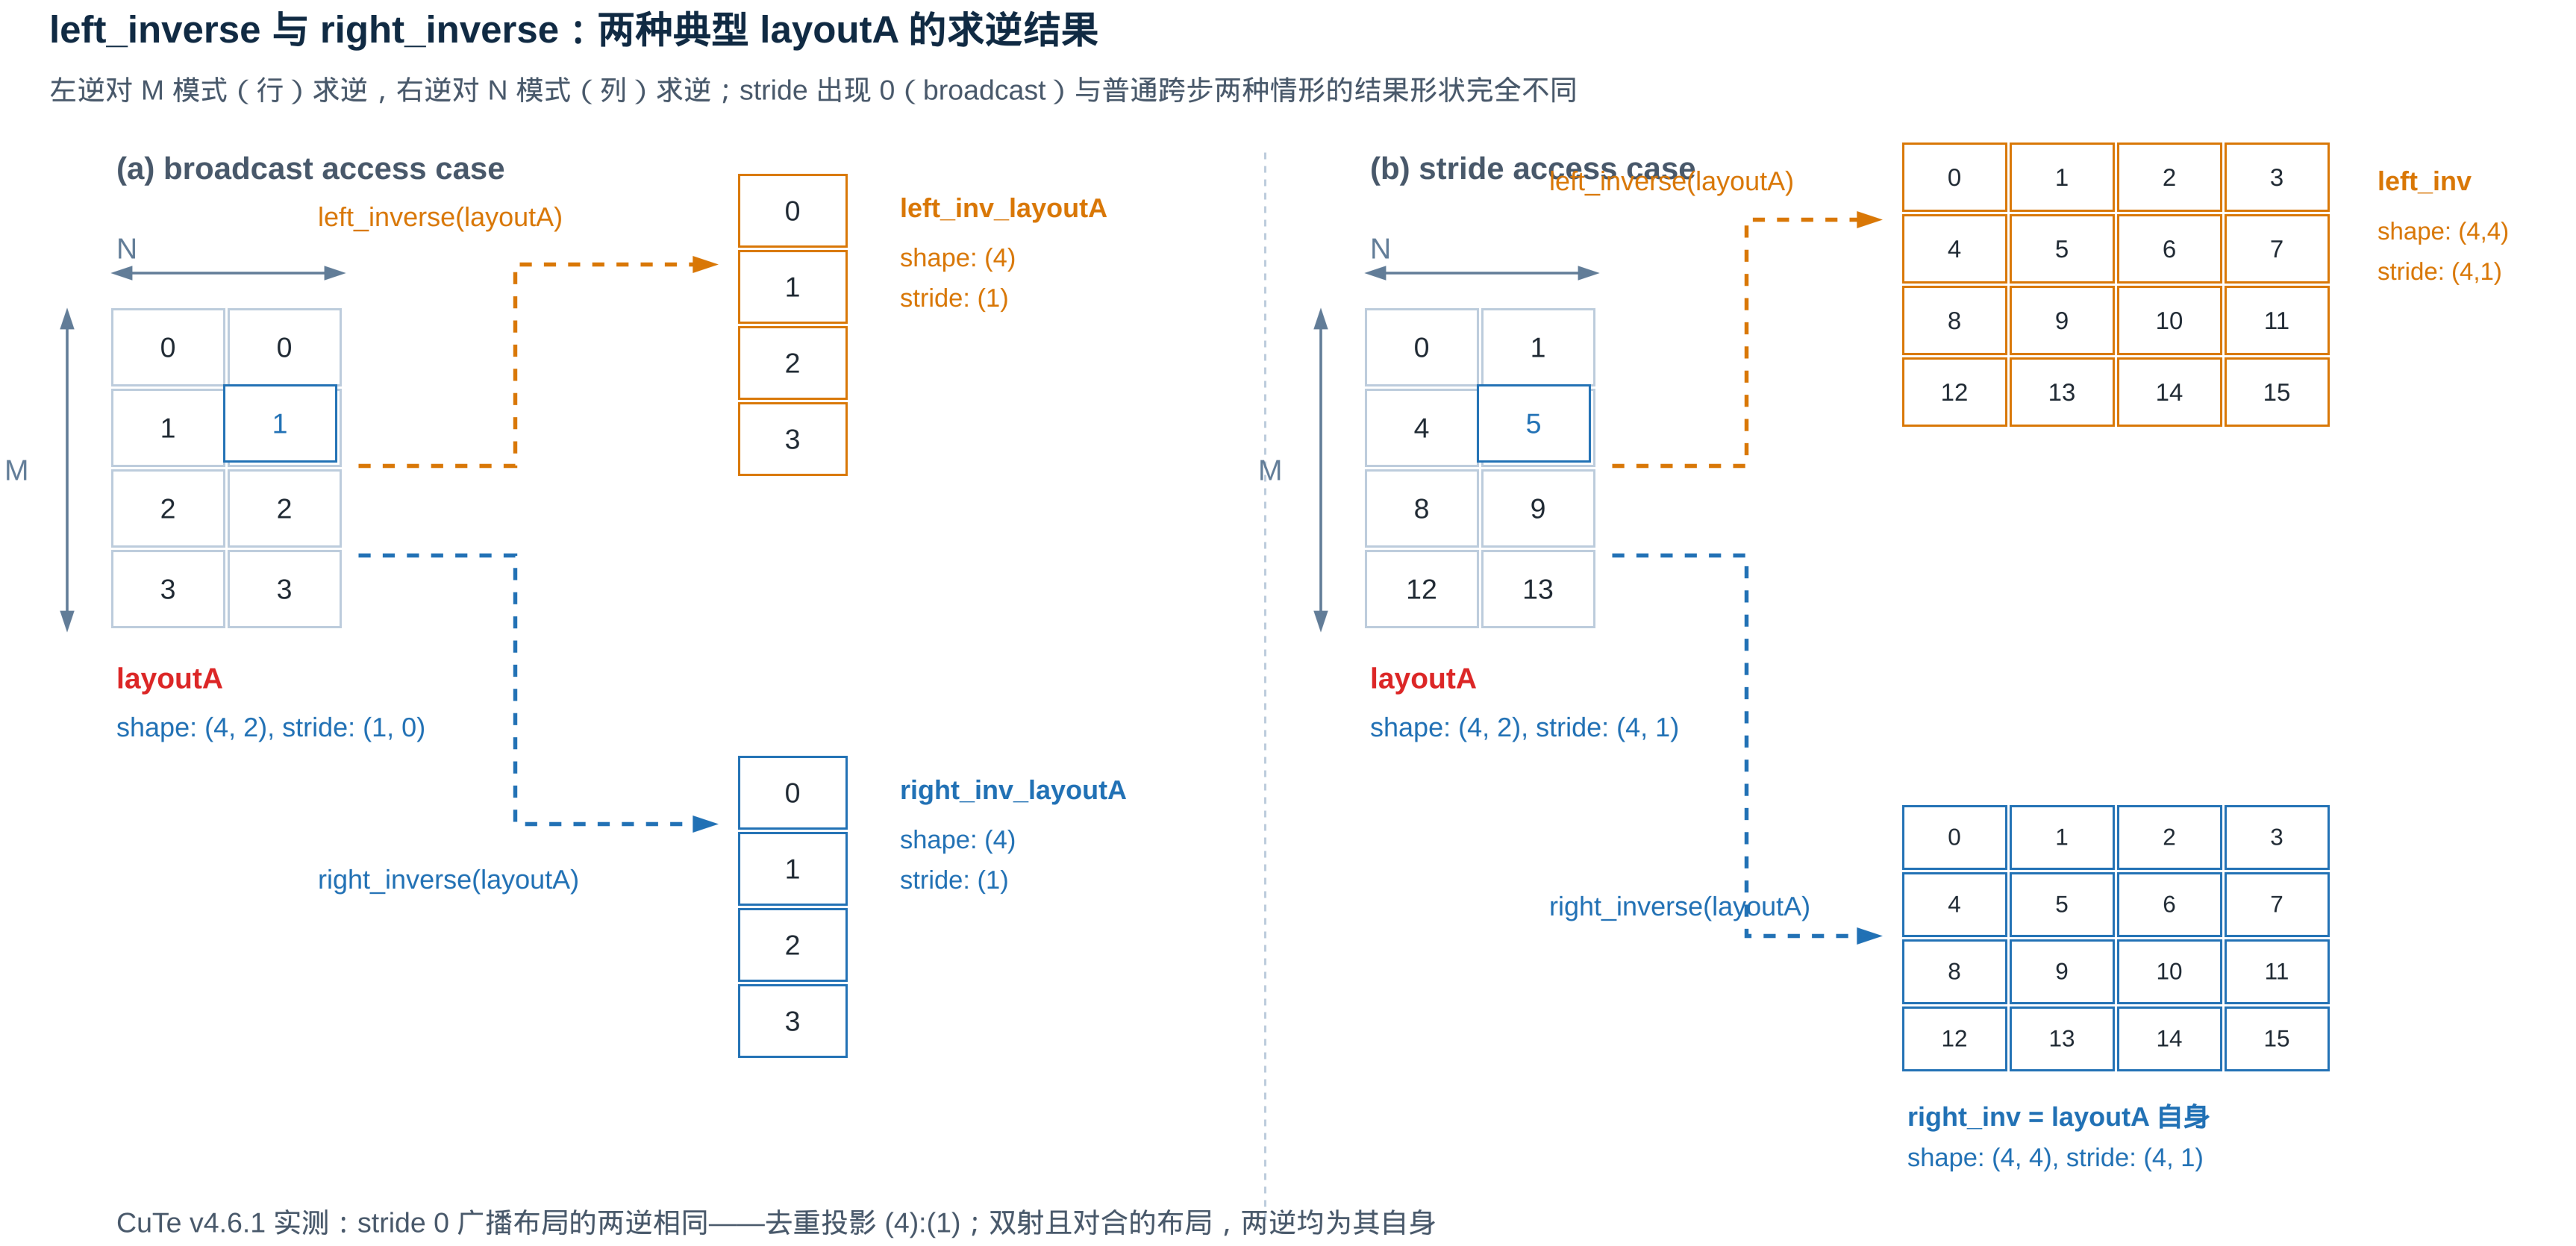
\includegraphics[width=0.95\textwidth]{figures/drawio/fig-20-7-left-right-inverse/fig-20-7.png}
\begin{tikzpicture}[font=\footnotesize, x=1cm, y=1cm,
    acell/.style={draw=gray!45, fill=white, minimum width=0.76cm, minimum height=0.535cm, inner sep=0pt},
    ahit/.style={draw=tkBlue, fill=white, text=tkBlue, minimum width=0.76cm, minimum height=0.535cm, inner sep=0pt}]
  % (a) broadcast case：layoutA 的 M 方向重复
  \begin{scope}[shift={(0.60, -2.06)}]
    \foreach \r in {0,...,3}{%
      \node[acell] at ({0.5*0.76}, {-\r*0.535-0.2675}) {\r};
      \node[acell] at ({1.5*0.76}, {-\r*0.535-0.2675}) {\r};}
    \node[ahit] at ({1.5*0.76}, {-1*0.535-0.2675}) {1};
    \draw[gray!70, {Stealth[length=2.5pt]}-{Stealth[length=2.5pt]}] (0, 0.34) -- ({2*0.76}, 0.34);
    \node[text=black!55, font=\scriptsize] at ({1*0.76}, 0.50) {$N$};
    \draw[gray!70, {Stealth[length=2.5pt]}-{Stealth[length=2.5pt]}] (-0.35, 0) -- (-0.35, {-4*0.535});
    \node[text=black!55, font=\scriptsize] at (-0.62, {-2*0.535}) {$M$};
  \end{scope}
  \node[anchor=west, text=tkRed] at (0.30, -4.55) {layoutA};
  \node[anchor=west, text=tkBlue] at (0.30, -4.86) {shape: $(4, 2)$, stride: $(1, 0)$};
  % (a) 的两逆：均为去重投影后的 1D (4):(1)
  \begin{scope}[shift={(4.70, -1.19)}]
    \foreach \r in {0,...,3}{\draw[tkOrange!80, fill=white] (0, {-\r*0.50}) rectangle (0.75, {-\r*0.50-0.50});}
    \foreach \r in {0,...,3}{\node at (0.375, {-\r*0.50-0.25}) {\r};}
  \end{scope}
  \begin{scope}[shift={(4.70, -5.20)}]
    \foreach \r in {0,...,3}{\draw[tkBlue, fill=white] (0, {-\r*0.50}) rectangle (0.75, {-\r*0.50-0.50});}
    \foreach \r in {0,...,3}{\node at (0.375, {-\r*0.50-0.25}) {\r};}
  \end{scope}
  \node[anchor=west, text=tkOrange!90!black, font=\scriptsize] at (2.00, -1.45) {left\_inverse(layoutA)};
  \node[anchor=west, text=tkOrange!90!black, font=\scriptsize] at (5.65, -1.25) {left\_inv\_layoutA};
  \node[anchor=west, text=tkOrange!90!black, font=\scriptsize] at (5.65, -1.55) {shape: $(4)$};
  \node[anchor=west, text=tkOrange!90!black, font=\scriptsize] at (5.65, -1.85) {stride: $(1)$};
  \node[anchor=west, text=tkBlue, font=\scriptsize] at (0.30, -5.60) {right\_inverse(layoutA)};
  \node[anchor=west, text=tkBlue, font=\scriptsize] at (5.65, -5.60) {right\_inv\_layoutA};
  \node[anchor=west, text=tkBlue, font=\scriptsize] at (5.65, -5.90) {shape: $(4)$};
  \node[anchor=west, text=tkBlue, font=\scriptsize] at (5.65, -6.20) {stride: $(1)$};
  % (b) stride case：layoutA 的双射跨步
  \begin{scope}[shift={(8.90, -2.06)}]
    \foreach \r in {0,...,3}{%
      \node[acell] at ({0.5*0.76}, {-\r*0.535-0.2675}) {\pgfmathparse{int(4*\r)}\pgfmathresult};
      \node[acell] at ({1.5*0.76}, {-\r*0.535-0.2675}) {\pgfmathparse{int(4*\r+1)}\pgfmathresult};}
    \node[ahit] at ({1.5*0.76}, {-1*0.535-0.2675}) {5};
    \draw[gray!70, {Stealth[length=2.5pt]}-{Stealth[length=2.5pt]}] (0, 0.34) -- ({2*0.76}, 0.34);
    \node[text=black!55, font=\scriptsize] at ({1*0.76}, 0.50) {$N$};
    \draw[gray!70, {Stealth[length=2.5pt]}-{Stealth[length=2.5pt]}] (-0.35, 0) -- (-0.35, {-4*0.535});
    \node[text=black!55, font=\scriptsize] at (-0.62, {-2*0.535}) {$M$};
  \end{scope}
  \node[anchor=west, text=tkRed] at (8.90, -4.55) {layoutA};
  \node[anchor=west, text=tkBlue] at (8.90, -4.86) {shape: $(4, 2)$, stride: $(4, 1)$};
  % (b) 左逆是 4x4 映射，右逆只覆盖值域起始的连续两项
  \begin{scope}[shift={(12.40, -1.10)}]
    \foreach \c in {0,...,3}{\foreach \r in {0,...,3}{%
      \pgfmathsetmacro\val{int(4*\r+\c)}%
      \draw[tkOrange!80, fill=white] ({\c*0.725}, {-\r*0.60}) rectangle ({\c*0.725+0.725}, {-\r*0.60-0.60});
      \node at ({\c*0.725+0.3625}, {-\r*0.60-0.30}) {\val};}}
  \end{scope}
  \begin{scope}[shift={(12.40, -5.20)}]
    \draw[tkBlue, fill=white] (0, 0) rectangle (0.75, -0.50);
    \draw[tkBlue, fill=white] (0, -0.50) rectangle (0.75, -1.00);
    \node at (0.375, -0.25) {0};
    \node at (0.375, -0.75) {4};
  \end{scope}
  \node[anchor=west, text=tkOrange!90!black, font=\scriptsize] at (11.60, -0.95) {left\_inverse(layoutA)};
  \node[anchor=west, text=tkOrange!90!black, font=\scriptsize] at (15.55, -1.30) {left\_inv};
  \node[anchor=west, text=tkOrange!90!black, font=\scriptsize] at (15.55, -1.60) {shape: $(4,4)$};
  \node[anchor=west, text=tkOrange!90!black, font=\scriptsize] at (15.55, -1.90) {stride: $(4,1)$};
  \node[anchor=west, text=tkBlue, font=\scriptsize] at (12.30, -4.95) {right\_inverse(layoutA)};
  \node[anchor=west, text=tkBlue, font=\scriptsize] at (12.40, -7.90) {right\_inv：$(2){:}(4)$};
  \node[anchor=west, text=tkBlue, font=\scriptsize] at (12.40, -8.20) {$R(0)=0,\quad R(1)=4$};
  % 求逆箭头（折线绕开文字）
  \draw[tkOrange!90!black, dashed, -{Stealth[length=3pt]}] (2.12, -2.20) -- (4.70, -1.69);
  \draw[tkBlue, dashed, -{Stealth[length=3pt]}]
    (2.12, -4.20) -- (3.90, -4.20) -- (3.90, -6.20) -- (4.70, -6.20);
  \draw[tkOrange!90!black, dashed, -{Stealth[length=3pt]}] (10.42, -2.60) -- (12.40, -2.30);
  \draw[tkBlue, dashed, -{Stealth[length=3pt]}]
    (10.42, -4.20) -- (12.10, -4.20) -- (12.10, -6.40) -- (12.40, -6.40);
  % 标题与脚注
  \node at (8.00, -0.19) {left\_inverse 与 right\_inverse：两种典型 layoutA 的求逆结果};
  \node[anchor=west, text=black!60, font=\scriptsize] at (0.30, -0.60)
    {左右逆由 $A\circ R$ 与 $R\circ A$ 的复合方向区分，不按 $M/N$ 模式分工；stride 为 0 与普通跨步会得到不同的定义域};
  \node[anchor=west, text=black!60, font=\scriptsize] at (0.30, -8.55)
    {CuTe v4.6.1 实测：广播布局的两逆均为 $(4){:}(1)$；跨步布局的左逆为 $(4,4){:}(4,1)$，右逆仅为 $(2){:}(4)$};
  \node[anchor=west, font=\scriptsize] at (0.30, -1.12) {(a) broadcast access case};
  \node[anchor=west, font=\scriptsize] at (8.90, -1.12) {(b) stride access case};
\end{tikzpicture}
\caption{left\_inverse / right\_inverse 的两种情形（CuTe v4.6.1 实测）：stride $(1,0)$ 广播布局的两逆相同，均为去重投影 $(4){:}(1)$。对 $A=(4,2){:}(4,1)$，左逆是 $(4,4){:}(4,1)$，而右逆只覆盖值域开头的连续两项，为 $(2){:}(4)$，即 $R(0)=0,R(1)=4$ 且 $A(R(i))=i$。左右逆由复合方向定义，不能按矩阵的 $M/N$ 模式理解。}
\label{fig:20-7}
\end{figure}

\begin{figure}[htbp]
\centering
\footnotesize
取 $A=B=(2,2){:}(2,1)$，则 CuTe 的 \texttt{logical\_product(A,B)} 为
\[
  P=((2,2),(2,2)){:}((2,1),(8,4)),\qquad
  P((a_0,a_1),(b_0,b_1))=2a_0+a_1+8b_0+4b_1 .
\]
\medskip
\begin{tabular}{c|rrrr}
\toprule
块坐标 $A$ / 网格坐标 $B$ & $(0,0)$ & $(1,0)$ & $(0,1)$ & $(1,1)$ \\
\midrule
$(0,0)$ & 0 & 8 & 4 & 12 \\
$(1,0)$ & 2 & 10 & 6 & 14 \\
$(0,1)$ & 1 & 9 & 5 & 13 \\
$(1,1)$ & 3 & 11 & 7 & 15 \\
\bottomrule
\end{tabular}
\caption{\texttt{logical\_product(A,B)} 的逐坐标求值：mode-0 是块 $A$，stride 为 $(2,1)$；mode-1 是网格 $B$，stride 为 $(8,4)$。它不同于直接拼接 \texttt{make\_layout(A,B)}（后者的 B 尚未按 $A$ 的 codomain 平移，不能把这里的 $(8,4)$ 直接当作拼接 stride），也不应按 $4A(c_A)+B(c_B)$ 解释。}
\label{fig:20-8}
\end{figure}

\begin{figure}[htbp]
\centering
% was: 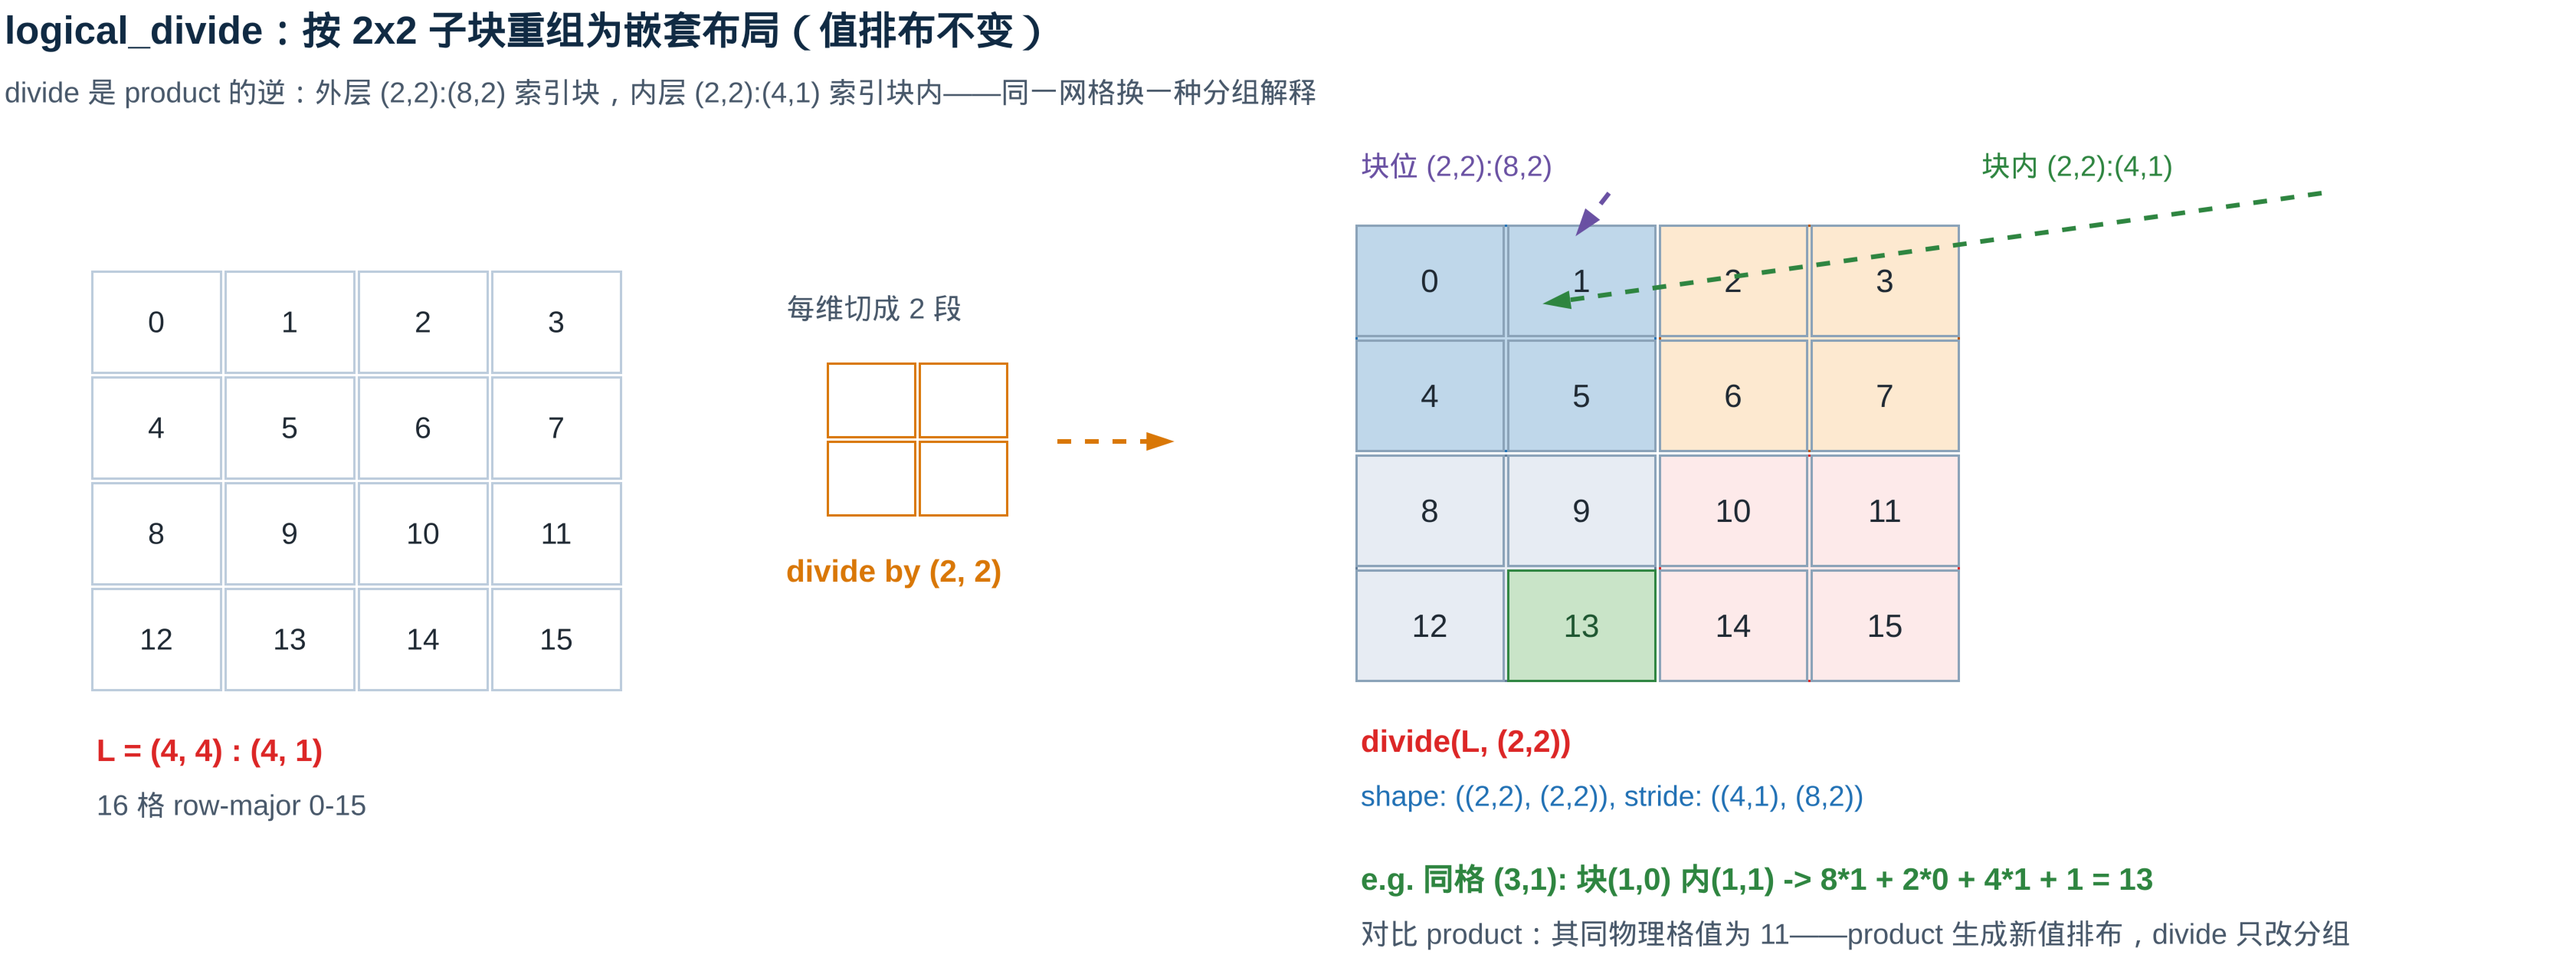
\includegraphics[width=0.95\textwidth]{figures/drawio/fig-20-9-layout-divide/fig-20-9.png}
\begin{tikzpicture}[font=\footnotesize, x=1cm, y=1cm]
  % 左：原始 row-major 4x4
  \begin{scope}[shift={(0.687, -1.76)}]
    \foreach \c in {0,...,3}{\foreach \r in {0,...,3}{%
      \pgfmathsetmacro\val{int(4*\r+\c)}%
      \draw[gray!45, fill=white] ({\c*0.866}, {-\r*0.68}) rectangle ({\c*0.866+0.866}, {-\r*0.68-0.68});
      \node at ({\c*0.866+0.433}, {-\r*0.68-0.34}) {\val};}}
  \end{scope}
  \node[anchor=west, text=tkRed] at (0.687, -4.74) {$L = (4, 4) : (4, 1)$};
  \node[anchor=west, text=black!60, font=\scriptsize] at (0.687, -5.07) {16 格 row-major 0--15};
  % 中：divide by (2,2) 的切块指示
  \begin{scope}[shift={(5.46, -2.36)}]
    \foreach \c in {0,1}{\foreach \r in {0,1}{\draw[tkOrange!80, fill=white] ({\c*0.567}, {-\r*0.478}) rectangle ({\c*0.567+0.567}, {-\r*0.478-0.478});}}
  \end{scope}
  \node[anchor=center, text=tkOrange!90!black] at (6.51, -3.70) {divide by $(2, 2)$};
  \node[anchor=center, text=black!60, font=\scriptsize] at (6.66, -2.00) {每维切成 2 段};
  \draw[tkOrange!90!black, dashed, -{Stealth[length=3pt]}] (6.96, -2.87) -- (7.70, -2.87);
  % 右：同一网格按 2x2 重新分组（值排布不变）
  \begin{scope}[shift={(8.90, -1.46)}]
    \fill[colorx1!20] (0, 0) rectangle ({2*0.985}, {-2*0.74});
    \fill[colorx3!20] ({2*0.985}, 0) rectangle ({4*0.985}, {-2*0.74});
    \fill[colorx5!20] (0, {-2*0.74}) rectangle ({2*0.985}, {-4*0.74});
    \fill[colorx7!20] ({2*0.985}, {-2*0.74}) rectangle ({4*0.985}, {-4*0.74});
    \foreach \c in {0,...,3}{\foreach \r in {0,...,3}{%
      \pgfmathsetmacro\val{int(4*\r+\c)}%
      \draw[gray!50] ({\c*0.985}, {-\r*0.74}) rectangle ({\c*0.985+0.985}, {-\r*0.74-0.74});
      \node at ({\c*0.985+0.4925}, {-\r*0.74-0.37}) {\val};}}
    \fill[tkFillGreen] (0.985, {-3*0.74}) rectangle ({2*0.985}, {-4*0.74});
    \draw[tkGreen, semithick] (0.985, {-3*0.74}) rectangle ({2*0.985}, {-4*0.74});
    \node[text=tkGreen!80!black] at ({1.5*0.985}, {-3.5*0.74}) {13};
    \draw[colorx1, semithick] (0, 0) rectangle ({2*0.985}, {-2*0.74});
    \draw[colorx3, semithick] ({2*0.985}, 0) rectangle ({4*0.985}, {-2*0.74});
    \draw[colorx5, semithick] (0, {-2*0.74}) rectangle ({2*0.985}, {-4*0.74});
    \draw[colorx7, semithick] ({2*0.985}, {-2*0.74}) rectangle ({4*0.985}, {-4*0.74});
  \end{scope}
  % 两个 mode 层级：块位（外）与块内（内）
  \node[anchor=west, text=tkPurple, font=\scriptsize] at (8.90, -1.00) {块位 $(2,2){:}(8,2)$};
  \node[anchor=west, text=tkGreen, font=\scriptsize] at (12.93, -1.00) {块内 $(2,2){:}(4,1)$};
  \draw[tkPurple, dashed, -{Stealth[length=3pt]}] (10.54, -1.25) -- (10.30, -1.42);
  \draw[tkGreen, dashed, -{Stealth[length=3pt]}] (15.16, -1.25) -- (10.15, -1.42);
  \node[anchor=west, text=tkRed] at (8.90, -4.78) {divide$(L, (2,2))$};
  \node[anchor=west, text=tkBlue] at (8.90, -5.14) {shape: $((2,2), (2,2))$,  stride: $((4,1), (8,2))$};
  \node[anchor=west, text=tkGreen, font=\scriptsize] at (8.90, -5.68)
    {e.g. 同格 $(3,1)$: 块$(1,0)$ 内$(1,1)$ $\to$ $8\times1 + 2\times0 + 4\times1 + 1 = 13$};
  \node[anchor=west, text=black!60, font=\scriptsize] at (8.90, -6.04)
    {对比 product：product 铺展生成新布局；divide 只重排已有布局的分组};
  % 标题
  \node at (8.00, -0.19) {logical\_divide：按 2x2 子块重组为嵌套布局（值排布不变）};
  \node[anchor=west, text=black!60, font=\scriptsize] at (0.09, -0.60)
    {外层 $(2,2){:}(8,2)$ 索引块、内层 $(2,2){:}(4,1)$ 索引块内；product 与 divide 并不互为逆运算};
\end{tikzpicture}
\caption{logical\_divide：按 $2\times2$ 子块把 $(4,4){:}(4,1)$ 重组为 $((2,2),(2,2)){:}((4,1),(8,2))$（CuTe 实测的 zipped 形式：块内 mode 在前、块位 mode 在后）——值排布不变（仍 row-major），改变的只是索引方式（一组 $(4,1)$ 索引块内、一组 $(8,2)$ 索引块位）。product 用块和网格生成新布局，divide 则重排已有布局，二者不能笼统称为互逆。}
\label{fig:20-9}
\end{figure}

\section{性能分析}

本章没有 kernel，性能一节只回答一个问题：这套代数要付多少代价？
答案是三点：编译期全折叠、运行期只剩加法与位运算、代价转移到编译时间。

\textbf{证据一（编译期折叠）}：static layout（所有 shape/stride 都是
\texttt{Int<N>}）上，\texttt{cosize}/\texttt{shape}/\texttt{compose}/
\texttt{divide} 的结果都是 \texttt{constexpr}。本章测试把
\texttt{tile\_\allowbreak{}to\_\allowbreak{}shape} 的结果直接写进了编译期断言：
\begin{lstlisting}
static_assert(cosize(decltype(atom){})  == 256,  "atom cosize folds");
static_assert(cosize(decltype(tiled){}) == 8192, "tiled cosize folds");
\end{lstlisting}
编译通过即证明：$128\times32\times2$ 的 smem 布局的全部尺寸计算没有进入
运行期一行代码。

\textbf{证据二（运行期退化为机器指令）}：compose/divide 之后的地址计算在
SASS 层面就是基址 + 若干次加法/移位。XOR swizzle 的复合在编译期折叠为
位运算，本章测试对 $8\times32$ 布局逐点核对了 \texttt{Swizzle\allowbreak{}<3,\allowbreak{}3,\allowbreak{}3>} 的复合
结果与位公式 $\mathrm{off}\oplus(((\mathrm{off}\gg6)\mathbin{\&}7)\ll3)$
完全一致（256 点、0 差异）。这与第~\ref{ch:12}~章手写 XOR 的
$30{,}720$ 点 v1/v2 等价性结论互相印证：声明式的 Swizzle $\circ$ layout
与手写位运算生成的是同一个函数。

\textbf{证据三（代码量口径）}：hgemm.cuh~L803--805 的注释声称手写版
$\sim$200 行、CuTe 版 $\sim$80 行。实测去注释非空行：手写 swizzle
kernel（L434--716）235 行；CuTe kernel 本体（L821--1196）118 行，另有 launch
wrapper（L1216--1427）86 行。所以注释里的 $\sim$80 行低估了 CuTe kernel 本体的物理
规模；实测支持的结论是\textbf{CuTe 版 kernel 里没有一行地址算术}：手写版用
\texttt{LDMATRIX\_X4}/\texttt{LDMATRIX\_X2}/\texttt{HMMA16816} 宏直接编排 PTX
与 lane 地址，CuTe 版的内联汇编为 0，地址全部由 layout 类型在编译期推出来。
绝对性能的端到端对照（TFLOPS）在第~\ref{ch:24}~章给出，本章不展开。

口径说明：本章测试是纯 host 断言（890 个），不产生 GPU 计时数据；上述
去注释行数口径为 \texttt{sed} 去注释与空行后的物理行数（2026-09-11 实测）。

\section{常见坑}

\textbf{坑一：坐标的 rank 必须匹配 shape 的嵌套结构。}
$\mathrm{make\_layout}(A,B)$ 的外层只有 2 个 mode（shape 为
$\bigl(\mathrm{shape}(A),$ $\mathrm{shape}(B)\bigr)$），
把它当 3 个 mode 索引
（如 \texttt{P(a0,a1,b)}）会直接编译失败：CuTe 会打印
\texttt{Mismatched Ranks}（\texttt{crd2idx} 的 \texttt{static\_\allowbreak{}assert}），
报错位置在 \texttt{stride.hpp}，第一次遇到时不容易定位问题所在。正确写法是
\texttt{P\allowbreak{}(make\_\allowbreak{}coord}\allowbreak\texttt{(a0,a1), b)}。另外：整数坐标可以展开
平坦的 shape（如 $(4,8)$），但不能展开嵌套元组，这是本章测试实际踩过的
编译错误。

\textbf{坑二：\texttt{make\_\allowbreak{}layout\allowbreak{}(Shape)} 默认 column-major。}它按
\texttt{LayoutLeft} 生成 stride（第一个 mode 变得最快），与 C 数组的
row-major 直觉相反。要 row-major 得写 \texttt{make\_\allowbreak{}layout\allowbreak{}(shape,\allowbreak{}
Layout\allowbreak{}Right\{\})} 或显式给 stride。

\textbf{坑三：用二维 Layout tiler 切几何块时，stride 必须与目标 layout 相容。}
$L=(8,8){:}(1,8)$ 上用 compact tile $(4,4){:}(1,4)$，得到的不是 $4\times4$
方块而是 16 个连续 offset 的条带。判别法与反例见 4.5 节实践须知；
shape-only 的 by-mode tiler 不走这条二维 Layout 路径。

\textbf{坑四：\texttt{right\_\allowbreak{}inverse} 对非满值域 layout 会静默退化。}
值域含空洞（如 stride 2）时返回平凡右逆 $(1){:}(0)$，不报错。判断标准：
$A$ 的像是否包含从 0 开始的连续段。需要恢复坐标时，通常用
\texttt{left\_\allowbreak{}inverse}（准逆，带 stride-0 歧义位）更合适。

\textbf{坑五：\texttt{Int<N>} 与 \texttt{int} 不只是优化开关。}
\begin{sloppypar}
动态值会让相关 layout 变成动态类型，编译期常量表达式（如
\texttt{static\_\allowbreak{}assert}\allowbreak\texttt{\allowbreak{}(cosize\allowbreak{}(.\allowbreak{}.\allowbreak{}.\allowbreak{}))}）无法求值，
运行期也会多出真实的算术。
kernel 里能用静态量就用静态量；这也解释了 hgemm 模板参数为什么写
\texttt{int BM, BN, BK} 再包成 \texttt{Int<BM>}（让上游保持可读、下游保持静态）。
\end{sloppypar}

\textbf{坑六：divide 结果的 shape 是嵌套的。}式~\eqref{eq:20-zd-example} 的
shape $\bigl((4,4),(2,2)\bigr)$ 是两个 mode、每个 mode 内含两个 mode，
不是 rank-4 的扁平 tuple。内层 mode 索引要按嵌套结构写（或用
\texttt{flatten}/\texttt{group} 显式展开）；本章测试用线性索引
\texttt{zd(t, r)} 能工作，是因为顶层恰好 rank 2 且内层是平坦 tuple。

\section{面试要点速查}

\textbf{Q1：CuTe 的 layout 是什么？为什么默认 column-major？}\\
A：layout 是坐标 $\to$ 线性 offset 的函数，由 (Shape, Stride) 表示，
$\mathrm{idx}=\sum_i d_i c_i$。默认 column-major（\texttt{LayoutLeft}）意味着
第一个 mode 变化最快。这是早年 BLAS 与 Tensor Core（如 MMA 的 m8n8 片段）
的通行约定，CuTe 全书沿用它；C 数组是 row-major，需要显式
\texttt{LayoutRight}。

\textbf{Q2：colex 是什么意思？整数坐标怎么参与？}\\
A：colex $=$ 坐标按最左 mode 最快的字典序枚举。把整数 $x$ 传给 layout 时，
CuTe 先用式~\eqref{eq:20-colex-decomp} 把 $x$ 分解回坐标，再算
$\sum d_i c_i$，所以线性索引与坐标是同一个函数的两种输入形式；
$f(x)$ 对 $x$ 一般不单调（row-major 即反例）。对 flat、非负 stride 的布局，
单调不减的充要条件是 mode-0 步进与各次 colex 进位的 offset 增量都非负；
compact col-major（$f(x)=x$）只是其中一个特例。

\textbf{Q3：compose 的定义与前提？}\\
A：$R=\mathrm{composition}(A,B)$ 满足 $R(c)=A(B(c))$，结果的 shape 与 $B$
相容（\texttt{compatible}，不要求逐字相同）。若要把结果化简为预期的普通
layout，还需满足 divisibility 和可表示性；静态布局不满足时通常触发编译期
断言，动态布局则仍需调用者保证。\texttt{coalesce\_x} 调整的是左操作数 $A$
的表示，并不改变 $A(B(c))$ 的函数语义。例：$(6,2){:}(9,2)\circ(4){:}(1)=(4){:}(9)$。

\textbf{Q4：右逆与左逆的区别？何时退化？}\\
A：右逆满足 $A(R(i))=i$（从 offset 找坐标），其 size 是 $A$ 的像中包含从 0 开始的最长连续前缀长度。
值域不满并不必然退化：图 20-7(b) 的像 $\{0,1,4,5\}$ 仍有非平凡右逆；只有像中从 0 开始的连续前缀
只剩 $\{0\}$（例如全偶 offset）时才退化为 $(1){:}(0)$。左逆是准逆 $A(R(A(c)))=A(c)$
（单射时为真左逆），用 stride-0 的 mode 编码多对一的歧义。colex compact（双射）时二者相等。

\textbf{Q5：分块（tile）在数学上是什么？}\\
A：\texttt{logical\_\allowbreak{}divide} $=$
$L\circ\mathrm{make\_layout}\bigl(T,$
$\mathrm{complement}(T,\mathrm{shape}(L))\bigr)$：
\begin{sloppypar}
tile 分量取 $T$、rest 分量取补空间；\texttt{zipped\_\allowbreak{}divide} 把结果整理成
(tile, rest) 两个 mode；\texttt{tiled} / \texttt{flat\_divide} 是展平变体。
当 $T$ 是连续单位 stride 块且整除时，可以把 $L$ 的地址空间写成
$\mathrm{size}(L)/\mathrm{size}(T)$ 块。一般情况下，rest 由
$\mathrm{complement}(T,\mathrm{shape}(L))$ 决定，不能笼统写成这个比值；
不整除时，结果 size 可能向上扩展，末块可能包含越界坐标。例如
$10{:}1$ 按 $4{:}1$ 分块得到 shape $(4,3)$、stride $(1,4)$，size 为 $12$。
\end{sloppypar}

\textbf{Q6：concatenation 与 product 家族有什么区别？}\\
A：\texttt{make\_\allowbreak{}layout(A,B)} 是 concatenation：直接拼接 mode，
坐标分量相加，不复制网格。product 家族包括 \texttt{logical\_\allowbreak{}product}
（block 铺在 tiler 上）、\texttt{blocked\_\allowbreak{}product}（重复 block）、
\texttt{raked\_\allowbreak{}product}（交错重复）与 \texttt{tile\_\allowbreak{}to\_\allowbreak{}shape}
（按目标 shape 铺 atom），区别在 block 之间怎么排。

\textbf{Q7：为什么说 CuTe 是零成本抽象？}\\
A：三点：static layout 的全部运算在编译期折叠（\texttt{static\_\allowbreak{}assert} 可证）；
运行期只剩加法/移位/位运算（swizzle 复合与手写位公式逐点一致）；
代价转移到编译时间与类型系统的复杂度。

\textbf{Q8：size 与 cosize 什么时候不等？}\\
A：对本书常见的单射、非负 stride 布局，stride 跳跃或 padding 引入空洞时
$\mathrm{cosize}>\mathrm{size}$，两者之差可表示额外的存储跨度。但这不是
双射或孔洞的充要条件：$(2,2,2){:}(1,1,5)$ 在
$\mathrm{size}=\mathrm{cosize}=8$ 时仍有重复和空洞。对常用非负 stride 的
smem 布局，\texttt{cosize} 是分配存储的依据，\texttt{size} 是逻辑坐标数。

\begin{sloppypar}
\textbf{Q9：FA2 里 C fragment 转 A fragment 需要什么样的 layout 变换？}\\
A：QK 的累加器按 C fragment 排布 $(\mathrm{MMA},\mathrm{MMA}_M,
\mathrm{MMA}_N)$，PV 的左操作数要 A fragment（形如
$((4,2),\mathrm{MMA}_M,\mathrm{MMA}_N/2)$），两者寄存器对齐不同、不能互当。
两条等价路线：tri-dao 的 \texttt{logical\_\allowbreak{}divide} 几何重排（本书
flash\_attn.cuh 的 \texttt{convert\_\allowbreak{}layout\_\allowbreak{}}\allowbreak\texttt{acc\_Aregs}
及复用它的 ffpa\_attn.cuh 采用，4.8 节），或 reed 的 inverse $+$ compose
代数链（更通用但依赖静态 stride）。
\end{sloppypar}

\section{最小测试与动手实验}

测试文件：\texttt{book/\allowbreak{}tests/\allowbreak{}ch20\_\allowbreak{}layout.\allowbreak{}cu}（host-only：不启动 kernel、
不需要 GPU；main 不调用任何 CUDA API）。八个 case 覆盖本章全部代数结论：
A 线性化（coord 与整数两种形式，128 断言）；B compose（14）；C right\_inverse
（65）；D left\_inverse（64）；E product（24）；F zipped\_divide（76，含双射
覆盖检查）；G tile\_to\_shape（261，含两条 \texttt{static\_\allowbreak{}assert} 编译期
折叠证明）；H Swizzle 复合（258，位公式逐点核对与 codomain 双射）。合计
890 个断言。

运行命令（在 \texttt{book/tests/} 下；\texttt{build\_\allowbreak{}tests.\allowbreak{}sh} 的
\texttt{INCLUDES} 已含仓库根的 \texttt{third-party/\allowbreak{}cutlass/\allowbreak{}include}，
直接运行即可）：

\begin{lstlisting}[style=console]
cd kernels/interview/book/tests
CUDA_VISIBLE_DEVICES=6 ./build_tests.sh --arch sm_120a --ch ch20
\end{lstlisting}

本机运行输出（RTX PRO 5000，CUDA 13.2，CUTLASS v4.6.1，2026-09-11）：

\begin{lstlisting}[style=console]
== ch20_layout.cu (sm_120a)
ch20 CuTe layout basics & algebra (host-only, no kernel launch)
PASS case A colex idx=sum(s_i*c_i): mismatches=0 (128 checks)
PASS case B composition R(c)==A(B(c)): mismatches=0 (14 checks)
PASS case C right_inverse L(R(i))==i: mismatches=0 (65 checks)
PASS case D left_inverse quasi-inverse: mismatches=0 (64 checks)
PASS case E product make_layout(A,B): mismatches=0 (24 checks)
PASS case F zipped_divide tile semantics: mismatches=0 (76 checks)
PASS case G tile_to_shape atom->(128,32,2): mismatches=0 (261 checks)
PASS case H Swizzle<3,3,3> o layout bit formula: mismatches=0 (258 checks)
ALL OK
\end{lstlisting}

判据说明：所有断言都是库计算与手工数学的逐点比较。例如 case A 的手工
一侧直接用 $\sum d_i c_i$ 与式~\eqref{eq:20-colex-decomp} 的展开式；case F 的
手工一侧用式~\eqref{eq:20-zd-coord}。任何一条不成立都会打印 FAIL 并以非零
退出码结束。动手实验（三条，都在本章测试上改）：

\begin{enumerate}
  \item 把 case F 的 $T$ 从 $(4,4){:}(1,8)$ 换成 compact 的 $(4,4){:}(1,4)$，
        观察结果变成 $\bigl((4,4),(4)\bigr){:}\bigl((1,4),(16)\bigr)$，
        理解 tile 语义依赖 stride 族。此时硬编码的坐标公式会 FAIL，但 compact
        结果仍是合法 layout，双射覆盖本身不应失败；这正是要区分的现象。
  \item 把 case B 的 $B$ 换成动态 shape（\texttt{int} 变量构造），观察
        \texttt{composition} 结果退化为运行期计算，理解静态/动态分水岭。
  \item 把 case H 的 \texttt{Swizzle\allowbreak{}<3,\allowbreak{}3,\allowbreak{}3>} 换成 \texttt{Swizzle\allowbreak{}<2,\allowbreak{}4,\allowbreak{}3>}
        或 \texttt{Swizzle\allowbreak{}<1,\allowbreak{}5,\allowbreak{}3>}，对照第~\ref{ch:12}~章的 SW64/SW128 档位
        公式，验证 $\langle$B,M,S$\rangle$ 三参数 $=$ 位域宽度的对应关系。
\end{enumerate}

\section*{延伸阅读}

\begin{itemize}
  \item @reed《cute 之 Layout》，
        \url{https://zhuanlan.zhihu.com/p/661182311}
        （(Shape,Stride) 与坐标映射的入门第一文，本章 3.1 节同源）；
  \item @reed《cute Layout 的代数和几何解释》，
        \url{https://zhuanlan.zhihu.com/p/662089556}
        （把 layout 运算解释成向量空间的代数结构，compose/divide 的几何直观）；
  \item @竹熙佳处《CuTe 教程：Layout Compose \& Inverse》，
        \url{https://zhuanlan.zhihu.com/p/1962625273636845008}
        （compose/inverse 的逐坐标推导与实例，本章 4.2/4.3 节的对照读物）；
  \item @竹熙佳处《CuTe 教程：Layout Product \& Divide》，
        \url{https://zhuanlan.zhihu.com/p/1971945267294111573}
        （product/divide 的图解与 kernel 用例，4.4/4.5 节对照）；
  \item @melonedo《Cute 布局代数实战：除法》，
        \url{https://zhuanlan.zhihu.com/p/1970274785691936058}
        （divide 在真实 kernel 里的用法与踩坑，与本章坑三互为印证）。
\end{itemize}

% ch21-cute-tensor-tiledcopy.tex — CuTe（二）：Tensor 与 TiledCopy（RFC-F F2，2026-09-11）
% \url 由 book.tex 的 hyperref 提供；单章独立编译时降级为可断行的 \ttfamily
% （逐字符插入 \allowbreak，避免长 URL 造成 Overfull \hbox）
\makeatletter
\providecommand{\urlchbrk}[1]{\@tfor\next:=#1\do{\next\allowbreak}}
\makeatother
\providecommand{\url}[1]{{\ttfamily\urlchbrk{#1}}}
\chapter{CuTe（二）：Tensor 与 TiledCopy}\label{ch:21}

\section{本章导读}

第~\ref{ch:20}~章把 layout 变成了一个可运算的对象：坐标怎么映到线性 offset、
两个布局怎么复合、怎么切分，全部由代数回答。但一个真实的 kernel 里还有第二类
问题：数据放在哪、由谁来搬。以第~\ref{ch:12}~章的手写 HGEMM 为例，
$128\times32$ 的 A tile 要经过三次搬运（gmem$\to$smem 的 \texttt{cp.async}、
smem$\to$寄存器的 \texttt{ldmatrix}、epilogue 的寄存器$\to$smem$\to$gmem），
每一次都有一份哪个线程搬哪几个元素的映射。这些映射散落在
\texttt{idx} 算术、lane 地址表与 shuffle 编排里，改一个 tile 尺寸就要重新推导。

本章引入 CuTe 的两个一等公民：\textbf{Tensor}（把数据指针 $+$ 布局绑成
一个对象）与 \textbf{TiledCopy}（把一个 copy 原子如何被多线程铺开形式化为
(thread, value) 二维网格）。四章路线中，本章位于第~\ref{ch:20}~章（layout
代数）与第~\ref{ch:22}~章（TiledMMA）之间：本章讲数据的搬运，第~\ref{ch:22}~章
讲计算的分区，第~\ref{ch:23}~章把两者接到硬件特性（Swizzle 与 TMA）上。

\textbf{前置章节}：第~\ref{ch:20}~章（compose/divide/product 与
\texttt{zipped\_\allowbreak{}divide}）、第~\ref{ch:11}~章（MMA fragment 与 ldmatrix）、
第~\ref{ch:12}~章（cp.async 与多级流水）。\textbf{源码区间}：
hgemm.cuh~L821--1196，即 Phase~7c-1 的 CuTe HGEMM kernel 本体（第~\ref{ch:24}~章
讲它的算法流程，本章只抽取其中的 Tensor/TiledCopy 用法）；需要时引用
L1216--1427 的 launch wrapper 中拷贝类型的构造段（G2S~L1303--1318、
S2R~L1319--1332、R2S~L1355--1362、S2G~L1364--1377），其中 L1232--1270 的
tile 尺寸与 SmemLayout 声明归第~\ref{ch:23}~章。\textbf{编译宏}：
\texttt{NOTES\_\allowbreak{}V2\_\allowbreak{}ENABLE\_\allowbreak{}CUTE}（需要 CUTLASS 头文件；sm80+ 均可编）。
配套最小测试 \texttt{book/\allowbreak{}tests/\allowbreak{}ch21\_\allowbreak{}tiled\_\allowbreak{}copy.cu}：host 端 TV-layout
断言，不启动 kernel。

\section{问题与动机}

第~\ref{ch:12}~章 swizzle 版 HGEMM 的主循环里，每个线程要搬到 smem 的 A 数据、
要从 smem 读进寄存器的 A/B fragment、epilogue 里要写回 gmem 的 C 元素，
各自都有一份映射：

\begin{enumerate}
  \item \textbf{G$\to$S}：128 个线程各搬 8 个 half（一条 128-bit \texttt{cp.async}）。
        线程 $t$ 搬哪 8 个需要手写：$m = t/4$、$n = 8\,(t \bmod 4) + v$。
  \item \textbf{S$\to$R}：\texttt{ldmatrix.x4} 的 lane 地址表：32 个 lane 各提供
        一行（或一列）的 smem 地址，硬件把 4 个 $8\times8$ 矩阵分发到寄存器；
        哪个 lane 指哪一行与 MMA fragment 布局绑定。
  \item \textbf{R$\to$S$\to$G}：accumulator fragment 在寄存器里的分布由
        m16n8k16 的 CLayout 决定，与 gmem 上连续无关；手写版要用
        \texttt{\_\_shfl\_sync} 跨 lane 收齐再写。
\end{enumerate}

三份映射必须彼此一致，而且它们\textbf{不是同一个函数}：G$\to$S 关心的是
gmem 合并访问与 smem 冲突，S$\to$R 关心的是 Tensor Core 的 fragment 约定，
R$\to$G 关心的是输出的写回形状。第~\ref{ch:11}、\ref{ch:12}~章的做法是
每个映射单独手写一遍，出错了靠对拍定位。

\begin{sloppypar}
CuTe 的做法是把这三件事统一成同一个抽象：一次拷贝 $=$ 一个
\emph{copy 原子}（一个线程搬多少元素、怎么排）$\times$ 一个
\emph{thread-value 划分}（第几个线程、第几个值对应数据的哪个坐标）。
TiledCopy 就是这个二元组的类型；\texttt{partition\_S} 与
\texttt{partition\_D} 负责按划分把源/目的 Tensor 切开，
\texttt{cute::copy} 负责逐元素执行，而两者的地址在编译期就已经折叠成
常量。本章要回答的四个问题：
\end{sloppypar}

\begin{itemize}
  \item \textbf{Tensor 是什么}：为什么指针必须与 layout 一起传递（3.1 节；4.1 节是它的
        kernel 实例）。
  \item \textbf{(thread, value) 怎么表达}：TV-layout 的定义、对偶与守恒律
        （3.3--3.5 节），以及它与第~\ref{ch:20}~章的 MN-layout 的关系。
  \item \textbf{TiledCopy 怎么来}：显式给 Thr/Val，或由 \texttt{TiledMMA}
        反推（\texttt{make\_\allowbreak{}tiled\_\allowbreak{}copy\_\allowbreak{}A/\allowbreak{}B/\allowbreak{}C}）（4.2--4.4 节）。
  \item \textbf{retile 为什么不需要搬数据}：零拷贝重标记的数学（3.7 节）。
\end{itemize}

\section{数学原理}

\subsection{Tensor：engine 与 layout}

第~\ref{ch:20}~章的 layout 只回答坐标 $\to$ offset，它不知道 offset 要加到
哪块内存上。访问数据的完整动作是两步：先算偏移，再把偏移加到基址上。

CuTe 把第二半的基址抽象成 Engine。@竹熙佳处给了一个好记的
类比：engine 之于 CuTe，相当于 iterator 之于 C++ 标准库，凡是
可以加偏移访问数据的实体都是 engine（gmem 指针、smem 指针、寄存器指针，
甚至一个纯坐标张量）。Engine 与 Layout 绑在一起，就是 Tensor：

\begin{equation}
  \mathrm{Tensor} = (\text{Engine},\ \text{Layout}), \qquad
  T(\mathbf{c}) = \mathrm{Engine}\bigl(:, \mathrm{Layout}(\mathbf{c})\bigr) ,
  \label{eq:21-tensor}
\end{equation}

用映射语言说：layout 负责 $(m,n)\to\mathrm{offset}$、engine 负责
$\mathrm{offset}\to$ 数据，Tensor 是两次映射的串联，这就是同一个
$(m,n)$ 坐标能落到 gmem/smem/reg 三种内存的原因：换 engine，layout
不用变（图~\ref{fig:21-1}）。

\begin{figure}[htbp]
\centering
% was: 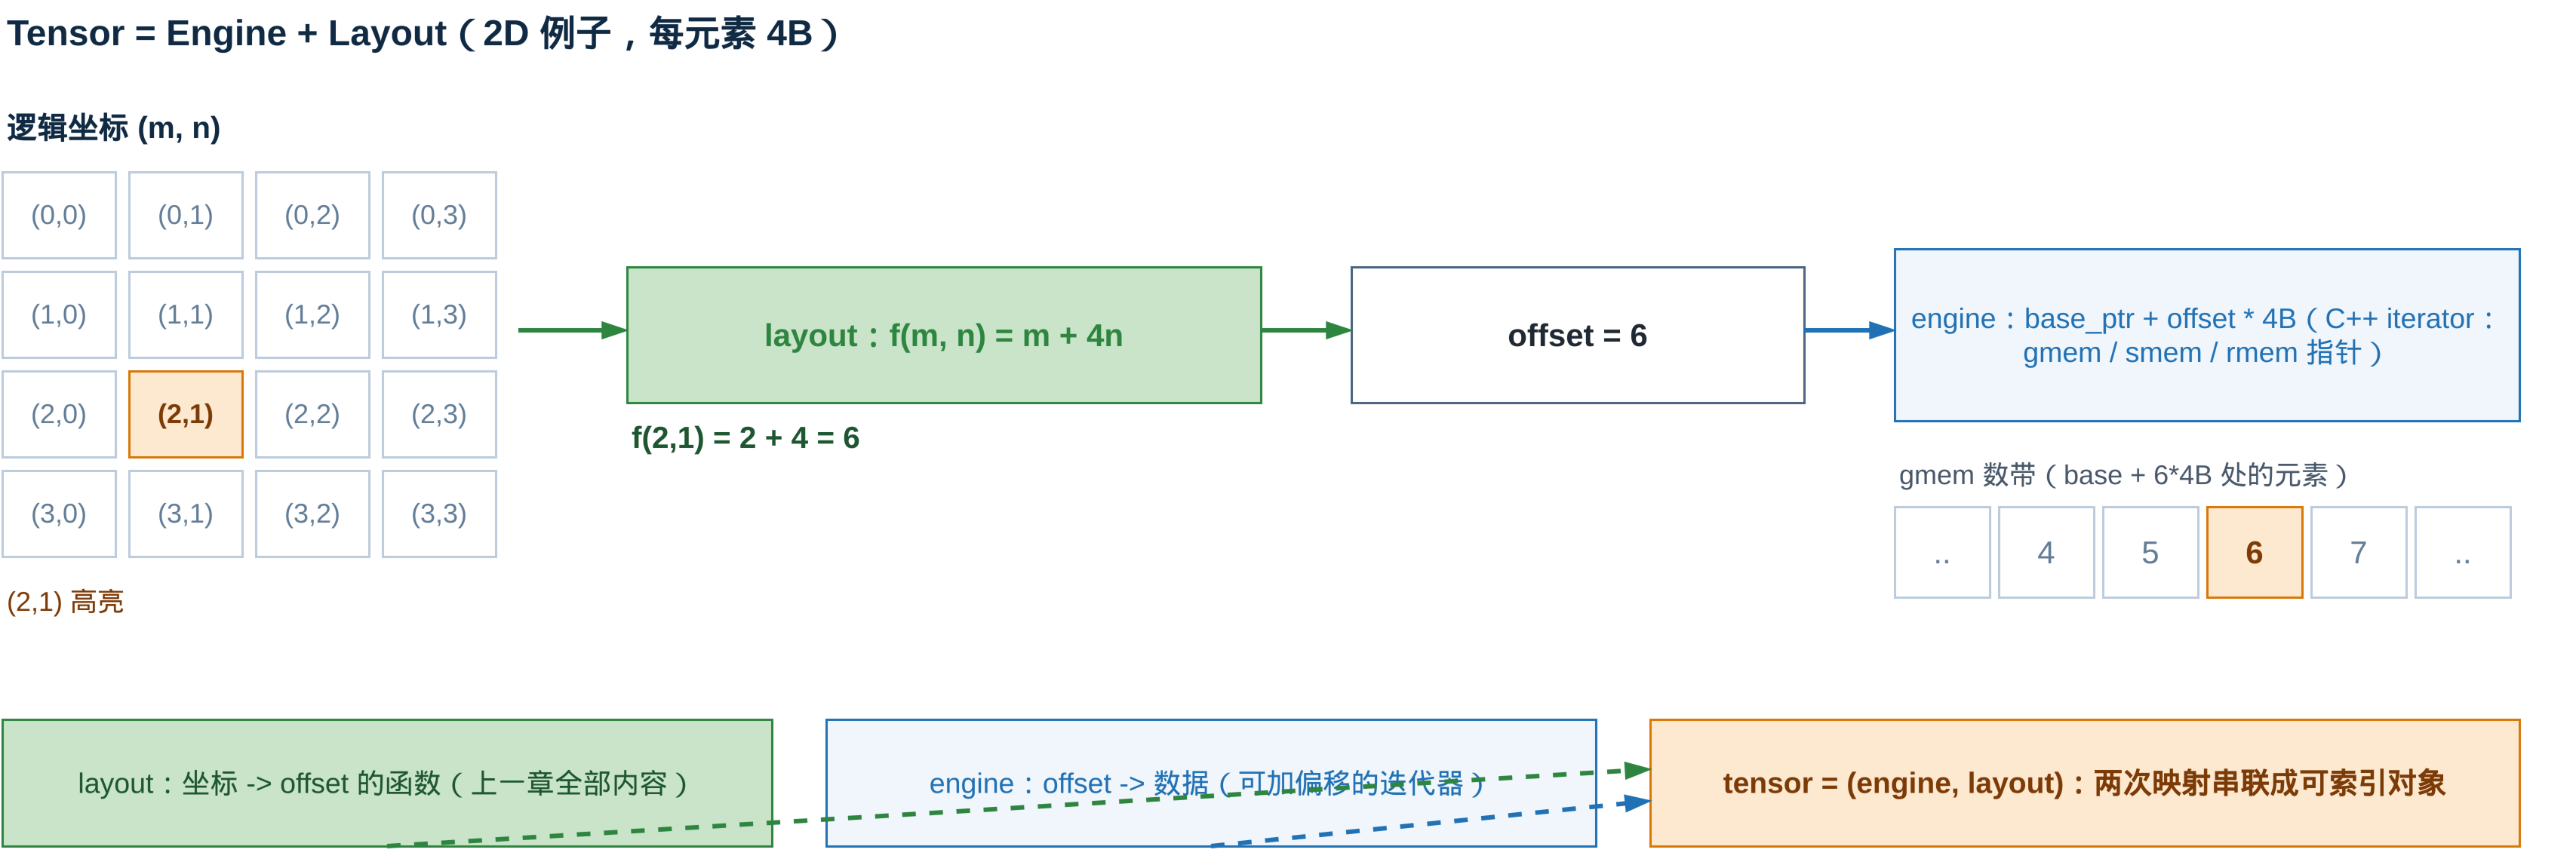
\includegraphics[width=0.95\textwidth]{figures/drawio/fig-21-1-engine-layout/fig-21-1.png}
\begin{tikzpicture}[font=\tiny, x=0.015cm, y=-0.015cm]
  \node[anchor=west, font=\scriptsize\bfseries] at (24,26)
    {Tensor = Engine + Layout（2D 例子，每元素 4B）};
  \node[anchor=west, font=\tiny\bfseries] at (24,68) {逻辑坐标 $(m, n)$};
  \foreach \rr in {0,...,3}{
    \foreach \cc in {0,...,3}{
      \node[draw=gray!45, fill=white, minimum width=0.75cm, minimum height=0.57cm,
            inner sep=0pt] at ({24+56*\cc+25},{88+44*\rr+19}) {$(\rr,\cc)$};
    }
  }
  \node[draw=tkOrange, fill=tkFillOrange, text=tkOrange!75!black, font=\tiny\bfseries,
        minimum width=0.75cm, minimum height=0.57cm, inner sep=0pt]
    at ({24+56+25},{88+88+19}) {$(2,1)$};
  \node[anchor=west, font=\tiny, text=tkOrange!75!black] at (24,278)
    {$(2,1)$ 高亮：它的偏移是这一格算出来的};
  \draw[-{Stealth[length=2mm]}, tkGreen, thick] (252,160) -- (297,160);
  \node[draw=tkGreen, fill=tkFillGreen, text=tkGreen!70!black, align=center,
        font=\scriptsize\bfseries, minimum width=4.2cm, minimum height=0.9cm,
        inner sep=1pt] at (440,160) {layout：$f(m, n) = m + 4n$};
  \node[anchor=north, font=\tiny\bfseries, text=tkGreen!70!black] at (440,196)
    {$f(2,1) = 2 + 4\cdot 1 = 6$};
  \draw[-{Stealth[length=2mm]}, tkGreen, thick] (580,160) -- (617,160);
  \node[draw=gray!70, fill=white, text=black, align=center,
        font=\scriptsize\bfseries, minimum width=3.0cm, minimum height=0.9cm,
        inner sep=1pt] at (720,160) {offset $= 6$};
  \draw[-{Stealth[length=2mm]}, tkBlue, thick] (820,160) -- (857,160);
  \node[draw=tkBlue, fill=tkFillBlue, text=tkBlue, align=center, font=\tiny,
        text width=3.8cm, minimum height=1.14cm, inner sep=2pt] at (998,160)
    {engine：\texttt{base\_ptr} $+$ offset $\times$ 4B（C++ iterator：gmem / smem /
     rmem 指针）};
  \node[anchor=west, font=\tiny] at (860,224) {gmem 数带（\texttt{base} $+$ $6\times4$B 处的元素）};
  \foreach \k/\v in {0/{..},1/{4},2/{5},3/{6},4/{7},5/{..}}{
    \node[draw=gray!45, fill=white, minimum width=0.63cm, minimum height=0.6cm,
          inner sep=0pt] at ({860+46*\k+21},256) {\v};
  }
  \node[draw=tkOrange, fill=tkFillOrange, text=tkOrange!75!black, font=\tiny\bfseries,
        minimum width=0.63cm, minimum height=0.6cm, inner sep=0pt]
    at ({860+46*3+21},256) {6};
  \node[draw=tkGreen, fill=tkFillGreen, text=tkGreen!70!black, align=center,
        font=\tiny, text width=4.7cm, minimum height=0.84cm, inner sep=2pt]
    at (194,358) {layout：坐标 $\to$ offset 的函数（上一章全部内容）};
  \node[draw=tkBlue, fill=tkFillBlue, text=tkBlue, align=center,
        font=\tiny, text width=4.7cm, minimum height=0.84cm, inner sep=2pt]
    at (558,358) {engine：offset $\to$ 数据（可加偏移的迭代器）};
  \node[draw=tkOrange, fill=tkFillOrange, text=tkOrange!75!black, align=center,
        font=\tiny\bfseries, text width=5.4cm, minimum height=0.84cm, inner sep=2pt]
    at (944,358) {tensor $=$ (engine, layout)：两次映射串联成可索引对象};
  \draw[-{Stealth[length=2mm]}, tkGreen, dashed, thick]
    (194,386) -- (194,400) -- (944,400) -- (944,388);
  \draw[-{Stealth[length=2mm]}, tkBlue, dashed, thick] (730,358) -- (748,358);
\end{tikzpicture}
\caption{Tensor 的两段结构：layout 把坐标映成偏移，engine 把偏移映成数据。同一个 layout 换不同 engine（gmem/smem/rmem/identity）就得到服务不同内存的 Tensor——这是第~\ref{ch:20}~章\textbf{布局与内存解耦}在 Tensor 上的体现。}
\label{fig:21-1}
\end{figure}

其中 Engine 是内存 $+$ 访问方式：\texttt{make\_\allowbreak{}gmem\_\allowbreak{}ptr\allowbreak{}(p)} 表示从全局
内存地址 $p$ 起算、\texttt{make\_\allowbreak{}smem\_\allowbreak{}ptr\allowbreak{}(p)} 表示 smem、\texttt{make\_\allowbreak{}rmem\_\allowbreak{}ptr}
表示寄存器、\texttt{make\_\allowbreak{}identity\_\allowbreak{}tensor} 返回坐标本身（本章测试用它做断言）。
\texttt{make\_\allowbreak{}tensor\allowbreak{}(ptr,\allowbreak{} shape,\allowbreak{} stride)} 是 hgemm CuTe 版里最常见的写法
（hgemm.cuh~L842--844）：\texttt{A[M][K]} 行主序存储，等价于
$\mathrm{Layout} = (M,K){:}(K,1)$。注意式~\eqref{eq:21-tensor} 里的 layout 可以
是任意复杂结构：只要能算出 offset，Tensor 就能寻址；这一点是后面
\texttt{partition\_S} 返回嵌套 mode 的 Tensor 仍然可用的原因。

Tensor 上最重要的两个操作在本章反复出现：

\begin{itemize}
  \item \textbf{切片/slice}：\texttt{tensor\allowbreak{}(coord)} 取单个元素，
        \texttt{tensor(\_, \_, k)} 用占位符 \texttt{\_} 保留某个 mode
        （得到低一维的视图），hgemm 里
        \texttt{gA(\_, \_, 0)} 表示第 0 个 K tile 的 $B_M\times B_K$ 视图。
  \item \textbf{局部切片/local\_tile}：\texttt{local\_\allowbreak{}tile\allowbreak{}(A,\allowbreak{} make\_\allowbreak{}tile\allowbreak{}(BM,\allowbreak{}BK),\allowbreak{}
        make\_\allowbreak{}coord\allowbreak{}(iy,\allowbreak{} \_\allowbreak{}))} 把大 Tensor 按 tile 切出当前 CTA 需要的那一块，
        同时保留未切出的 remainder mode，它的实现就是第~\ref{ch:20}~章
        的 \texttt{zipped\_\allowbreak{}divide}（L852--854 的 gA/gB/gD）。
\end{itemize}

\subsection{小例子：4 个线程搬一块 $(4,4)$}

在进入公式之前，先按 @竹熙佳处的建议走一遍最小场景：\emph{一个 threadblock
要把一块 $(k_{\mathrm{TileM}},k_{\mathrm{TileN}})$ 的数据从 src 搬到 dst}
（g2s / s2r / s2g 同理）。为了能手算，取 4 个线程、$(4,4)$ 的 tile、
每线程每轮搬 2 个连续元素。

朴素 CUDA 的教科书式写法是：每个线程按 tid 算出自己的
src/dst 地址；让连续线程读连续地址（合并访存）；让每线程一次搬多个元素
（宽访存）。4 线程 $\times$ 2 float $= 8$ 个元素一轮，$4\times4=16$ 个元素
循环 2 轮：

\begin{lstlisting}
  int tid = threadIdx.x;              // 0..3
  int r = tid / 2;                    // 行方向线程号
  int c = (tid % 2) * 2;              // 列方向起点（每线程 2 个连续 float）
  for (int loop = 0; loop < 2; ++loop) {            // 16 / (4*2) = 2 轮
    float2 s = *(float2*)&g[(loop * 2 + r) * 4 + c];    // src: 合并访存
    *(float2*)&shm[(loop * 2 + r) * 4 + c] = s;         // dst: 无冲突写
  }
\end{lstlisting}

\textbf{问题在哪。}这段代码很短，但它把谁搬哪块\emph{算在了}
\texttt{r}/\texttt{c}/\texttt{loop} 三个变量里。一旦引入 swizzle、
ldmatrix 或 bank 冲突考虑，地址公式会迅速膨胀，而哪个数据在哪个线程
手里会彻底看不清。@竹熙佳处建议先把映射从代码里抽出来画成一张
表：行是线程号 $t$，列是线程内的值号 $v$，格子填数据坐标 $(m,n)$，
这张表就是图~\ref{fig:21-2} 的左半。

从这张表可以读出两件事：

\begin{itemize}
  \item \textbf{写代码用的是反向的那张表}：我们想的从来不是数据
        $(0,1)$ 归谁，而是\emph{线程 0 的值 1 去哪取}，把行列对调
        看一次，就是第~\ref{ch:20}~章 inverse 运算的内容。CuTe 的
        TV-layout 直接以 $(t,v)\to$ 坐标的形式存储，就是这张对调后的表。
  \item \textbf{引入更多优化后，表仍然存在}（只是格子里要额外多经一层 swizzle、
        ldmatrix 的地址映射）。表画得出来，说明这个映射是独立于循环
        代码的对象，把它变成 layout，地址计算就交给编译器推导。
\end{itemize}

\begin{figure}[htbp]
\centering
% was: 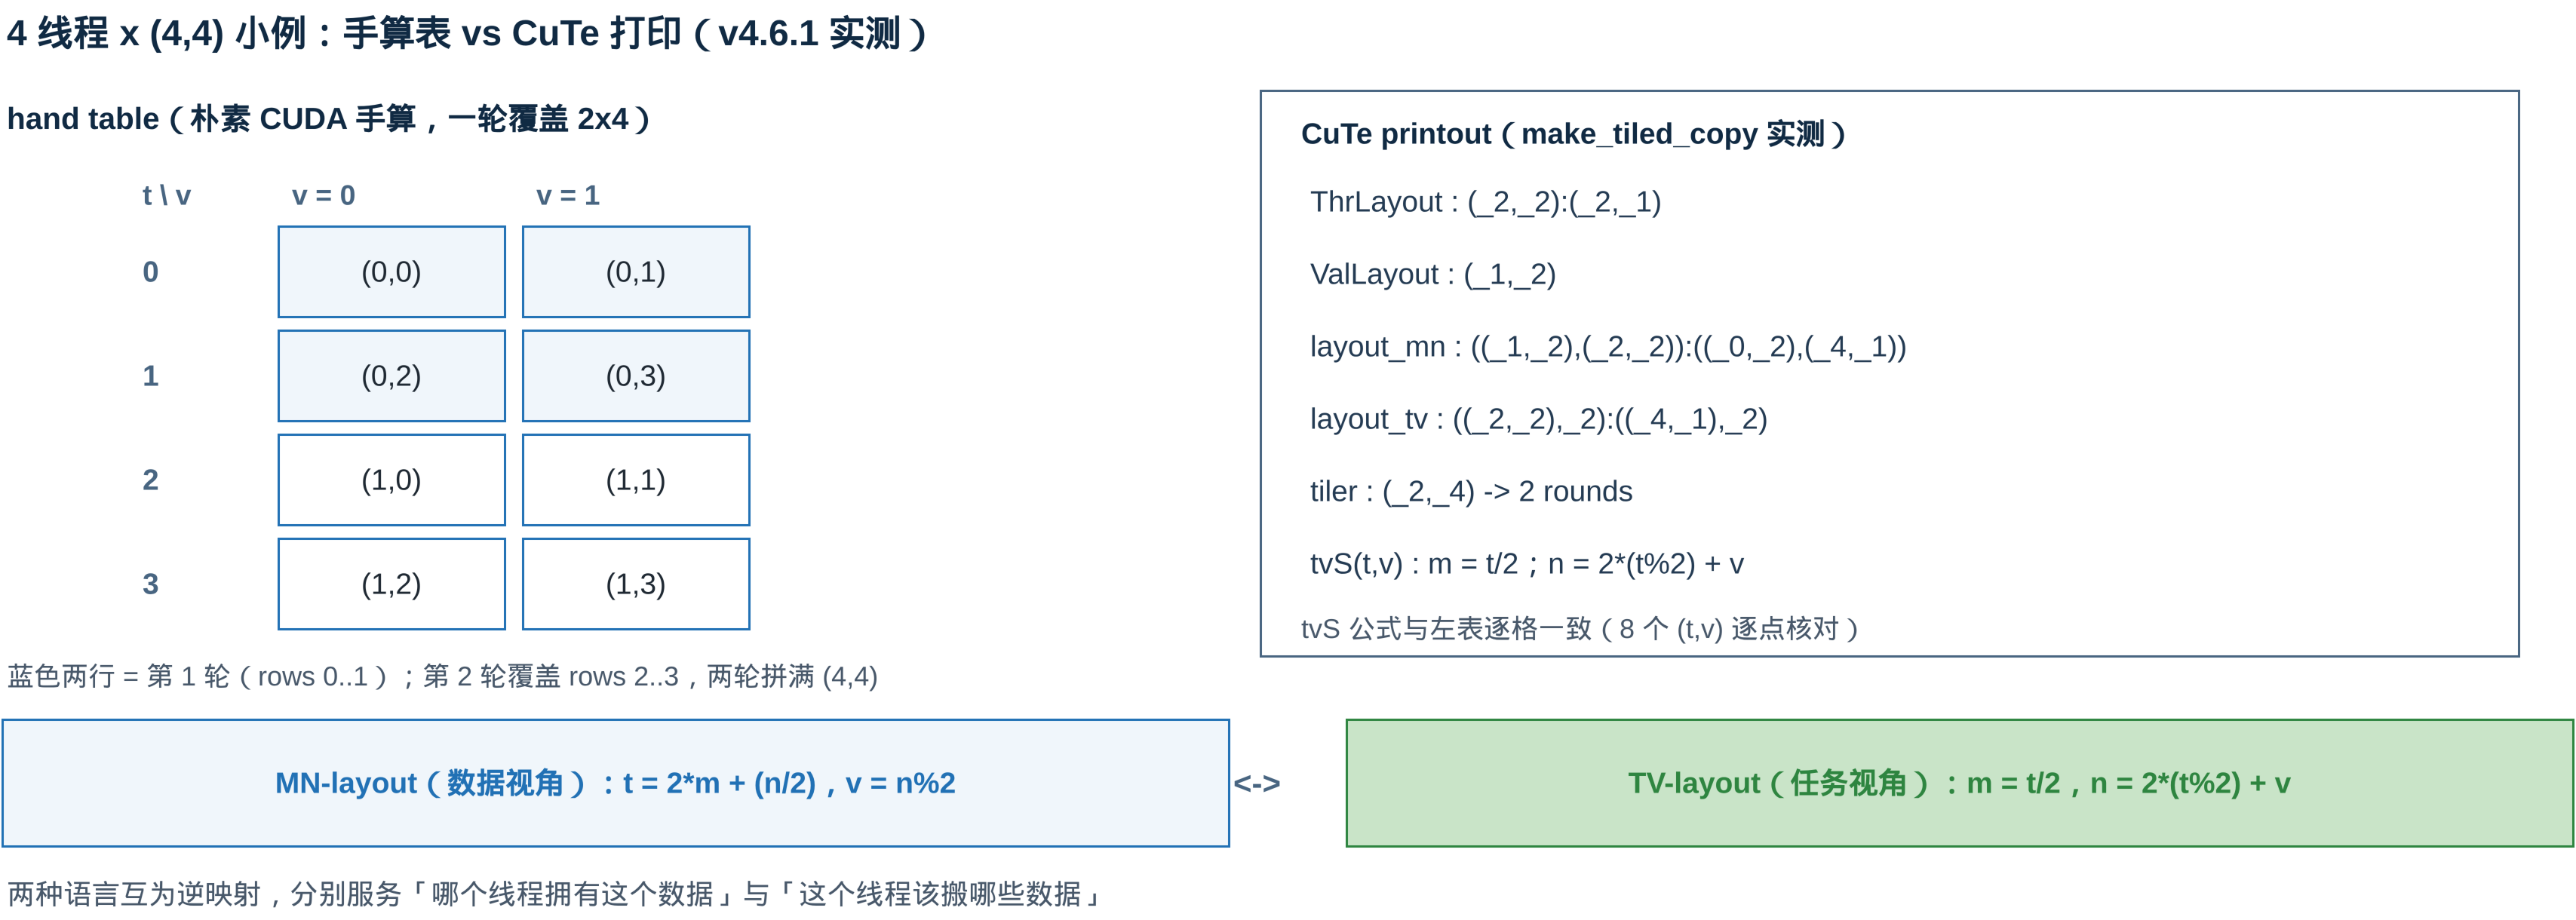
\includegraphics[width=0.95\textwidth]{figures/drawio/fig-21-2-tv-table/fig-21-2.png}
\begin{tikzpicture}[font=\tiny, x=0.015cm, y=-0.015cm]
  \node[anchor=west, font=\scriptsize\bfseries] at (24,26)
    {4 线程 $\times$ $(4,4)$ 小例：手算表 vs CuTe 打印（v4.6.1 实测）};
  \node[anchor=west, font=\tiny\bfseries] at (24,64)
    {hand table（朴素 CUDA 手算，一轮覆盖 $2\times4$）};
  \node[font=\tiny\bfseries] at (114,98) {$t \backslash v$};
  \node[font=\tiny\bfseries] at (200,98) {$v = 0$};
  \node[font=\tiny\bfseries] at (308,98) {$v = 1$};
  \foreach \rr in {0,...,3}{
    \pgfmathtruncatemacro{\mm}{int(\rr/2)}
    \pgfmathtruncatemacro{\nb}{2*mod(\rr,2)}
    \node[draw=gray!45, fill=white, minimum width=0.75cm, minimum height=0.36cm,
          inner sep=0pt] at (109,{132+46*\rr}) {$\rr$};
    \foreach \cc in {0,1}{
      \pgfmathtruncatemacro{\nn}{\nb+\cc}
      \ifnum\rr<4
        \node[draw=tkBlue, fill=tkFillBlue, minimum width=1.5cm, minimum height=0.6cm,
              inner sep=0pt] at ({196+108*\cc},{132+46*\rr}) {$(\mm,\nn)$};
      \else
        \node[draw=tkBlue, fill=white, minimum width=1.5cm, minimum height=0.6cm,
              inner sep=0pt] at ({196+108*\cc},{132+46*\rr}) {$(\mm,\nn)$};
      \fi
    }
  }
  \node[anchor=west, font=\tiny] at (24,311)
    {蓝色四行 $=$ 4 个线程全体；第 1 轮共同覆盖数据行 $m=0,1$，第 2 轮覆盖 $m=2,3$};
  \draw[gray!60, thin] (580,52) rectangle (1136,302);
  \node[anchor=west, font=\tiny\bfseries] at (596,71)
    {CuTe printout（\texttt{make\_tiled\_copy} 实测）};
  \foreach \k/\t in {0/{ThrLayout : (\_2,\_2):(\_2,\_1)},
                     1/{ValLayout : (\_1,\_2)},
                     2/{layout\_mn : ((\_1,\_2),(\_2,\_2)):((\_0,\_2),(\_4,\_1))},
                     3/{layout\_tv : ((\_2,\_2),\_2):((\_4,\_1),\_2)},
                     4/{tiler\phantom{X}: (\_2,\_4) $\to$ 2 rounds},
                     5/{tvS(t,v)  : $m = t/2$；$n = 2(t\bmod 2) + v$}}{
    \node[anchor=west, font=\tiny] at (600,{101+32*\k}) {\texttt{\t}};
  }
  \node[anchor=west, font=\tiny] at (596,290)
    {tvS 公式与左表逐格一致（8 个 $(t,v)$ 逐点核对）};
  \node[draw=tkBlue, fill=tkFillBlue, text=tkBlue, align=center, font=\tiny,
        text width=7.7cm, minimum height=0.84cm, inner sep=2pt] at (295,358)
    {MN-layout（数据视角）：$t = 2m + (n/2)$，$v = n \bmod 2$};
  \node[font=\scriptsize\bfseries] at (592,358) {$\leftrightarrow$};
  \node[draw=tkGreen, fill=tkFillGreen, text=tkGreen!70!black, align=center, font=\tiny,
        text width=7.7cm, minimum height=0.84cm, inner sep=2pt] at (889,358)
    {TV-layout（任务视角）：$m = t/2$，$n = 2(t \bmod 2) + v$};
  \node[anchor=west, font=\tiny] at (24,407)
    {两种语言互为逆映射，分别服务\textbf{哪个线程拥有这个数据}与\textbf{这个线程该搬哪些数据}};
\end{tikzpicture}
\caption{4 线程小例子的两种表格：左边是朴素 CUDA 手算的\textbf{线程 $\times$ 值 $\to$ 坐标}表（一轮覆盖 $2\times4$、两轮铺满 $(4,4)$），右边是 CuTe 的 \texttt{make\_\allowbreak{}tiled\_\allowbreak{}copy} 打印结果——\texttt{tvS} 的公式与手算逐格一致。MN-layout 与 TV-layout 互为逆映射，分别服务\textbf{数据视角}与\textbf{线程视角}。}
\label{fig:21-2}
\end{figure}

把这个小表放大到真实体量（128 线程、每线程 8 个
half、$32\times32$ 的 tile），就得到 hgemm 的 G$\to$S 划分：\texttt{ThrLayout}
从 $(2,2){:}(2,1)$ 变成 $(32,4){:}(4,1)$，\texttt{ValLayout} 从 $(1,2)$ 变成
$(1,8)$，$t$/$v$ 的公式就是 3.4 节的式~\eqref{eq:21-g2s-tv}。

\subsection{(thread, value) 网格：TV-layout}

一次由 $P$ 个线程执行、每线程搬 $V$ 个值的拷贝，本质上是把 tile 的每个坐标
指派给一个二元组 $(t,v)\in[0,P)\times[0,V)$。CuTe 把这个指派本身写成一个
layout，称为 \textbf{TV-layout}：

\begin{equation}
  \mathrm{TV}:\ (t,v) \longmapsto (\text{tile 内坐标}), \qquad
  \text{逆映射 } \mathrm{MN}:\ (\text{坐标}) \longmapsto (t,v) .
  \label{eq:21-tv}
\end{equation}

TV 与 MN 是\textbf{同一个划分的两种视角}：写 kernel 时我们关心第 $t$ 个线程
拿哪几个值（TV），写布局时我们关心坐标 $(m,n)$ 落在谁手上（MN）。
CuTe 两个方向都提供，并且用同一个 layout 表示：

\begin{equation}
  \mathrm{Layout\_TV} \;=\; \bigl(\mathrm{Layout\_MN}\bigr)^{-1}
  \ \text{（右逆）}, \qquad
  \mathrm{Tiler} = \mathrm{product\_each}\bigl(\mathrm{shape}(\mathrm{Layout\_MN})\bigr) .
  \label{eq:21-mn-tv}
\end{equation}

\subsection{raked\_product：从 Thr/Val 到 MN}

上节小例子里我们直接画了表；在 CuTe 里，画表被拆成两个更好写的动作：
声明线程怎么排（ThrLayout）、声明每线程搬的值怎么排（ValLayout），
再由 \texttt{make\_\allowbreak{}tiled\_\allowbreak{}copy} 合成完整的 MN 表。
\texttt{make\_\allowbreak{}tiled\_\allowbreak{}copy\allowbreak{}(atom,\allowbreak{} Thr\allowbreak{}Layout,\allowbreak{} Val\allowbreak{}Layout)} 的两个需要手动指定的参数是
坐标$\to$thr/val 的两个函数（注意方向：它们把坐标映到线程号/值号，
不是反过来）：

\begin{align}
  \mathrm{ThrLayout}&:\ (i,j) \longmapsto t = 4i + j, \qquad
  \mathrm{ValLayout}:\ (i,j) \longmapsto v = j , \label{eq:21-g2s-params}
\end{align}

式~\eqref{eq:21-g2s-params} 就是 hgemm 的 G$\to$S 参数
（hgemm.cuh~L1313--1317：\texttt{Thr\allowbreak{}Layout\ =\allowbreak{}\ \allowbreak{}(32,\allowbreak{}4){:}\allowbreak{}(4,\allowbreak{}1)}、
\texttt{ValLayout\ =\ (1,8)}）。CuTe 把它们合成一个 MN 布局
\begin{equation}
  \mathrm{Layout\_MN} = \mathrm{raked\_product}\bigl(
    \mathrm{ThrLayout},\ \mathrm{ValLayout}\bigr)
  \ =\ \bigl((1,32),(8,4)\bigr){:}\bigl((0,4),(128,1)\bigr),
  \label{eq:21-raked}
\end{equation}
右侧为 CuTe 的实测输出形式（按 $(t,v)$ 的 colex 编码 $t+128v$ 索引
线程-值对）。其中 \texttt{raked}（交错）指：同一个线程的 $V$ 个值沿坐标连续排列，
而不是把 tile 先按线程切成大块、再在线程内切小块（回看 3.2 节的小例子：
Thr \texttt{(2,2):(2,1)} 与 Val \texttt{(1,2)} 按同样方式合成出来的，正是
那张手画的表）。式~\eqref{eq:21-raked} 的最简版本就是 kernel 注释里的
\textbf{128 个线程，每线程搬运 1$\times$8=8 个 half}（hgemm.cuh~L1308--1309）。

把式~\eqref{eq:21-raked} 按坐标写开：坐标 $(i,j')$
（$i\in[0,32)$、$j'\in[0,32)$）满足 $j' = 8j+v$，于是

\begin{equation}
  \boxed{\ t = 4i + j = 4i + \Bigl\lfloor \frac{j'}{8}\Bigr\rfloor,
  \qquad v = j' \bmod 8\ }
  \label{eq:21-g2s-mn}
\end{equation}

反过来（线程视角，本章测试 case~A 逐点核对的那条）：
\begin{equation}
  i = \Bigl\lfloor \frac{t}{4}\Bigr\rfloor,\qquad
  j' = 8\,(t \bmod 4) + v .
  \label{eq:21-g2s-tv}
\end{equation}

读法：线程 $t$ 负责第 $\lfloor t/4\rfloor$ 行的第 $8(t\bmod 4)$
到 $8(t\bmod 4)+7$ 列，即连续 8 个元素，正好对齐一条 128-bit \texttt{cp.async}。
这就是 G$\to$S 划分的结论，它在手写版里是两行 $\mathrm{idx}$ 算术，
在 CuTe 里是式~\eqref{eq:21-raked} 的类型。

\subsection{守恒律与重复因子}

由式~\eqref{eq:21-mn-tv} 右逆的定义，TV 布局天然把
$P\times V$ 个 $(t,v)$ 映射到 Tiler 上；当它是双射时立刻得到一条守恒律：

\begin{equation}
  P \times V = \bigl|\mathrm{Tiler}\bigr| = \prod_i \mathrm{size}_i .
  \label{eq:21-conserve}
\end{equation}

G$\to$S 的实测：$P\times V = 128\times 8 = 1024 = 32\times 32 = |\mathrm{Tiler}|$
（3.4 节的 Thr/Val 恰好把 $32\times32$ 的 tile 铺满一层）。S$\to$R 的实测则
不同：\texttt{make\_\allowbreak{}tiled\_\allowbreak{}copy\_\allowbreak{}A} 得到的 tiler 是
$(\mathrm{tile\_size}_0, \mathrm{tile\_size}_2) = (32,16)$，只有 512 个元素，
而 $P\times V = 128\times 8 = 1024$，即 2 倍的重复因子。原因不是 bug：
$2\times2$ 的 warp 排布里，两个 N 方向的 warp 需要同一份 A fragment，
于是同一块 A 数据被两组线程各读一遍。一般地：

\begin{equation}
  \text{A 的重复因子} = \#\{\text{N 方向 warp}\},\qquad
  \text{B 的重复因子} = \#\{\text{M 方向 warp}\} .
  \label{eq:21-dup}
\end{equation}

式~\eqref{eq:21-dup} 是后面理解 fragment 寄存器占用的关键：本章测试 case~E
对 A 拷贝的 128$\times$32 tile 做覆盖统计，实测每个元素恰好被 2 个
(thread, value) 对覆盖（$\mathrm{multi}=8192$ 个覆盖点、$\mathrm{once}$ 结构
$4096/2$），与式~\eqref{eq:21-dup} 完全一致。该覆盖结构的网格化见
图~\ref{fig:21-s2r-dup}。

\begin{figure}[H]
\centering
\begin{tikzpicture}[font=\tiny]
  \def\cwd{0.5}
  \def\chh{0.3}
  \foreach \fm in {0,...,31}{
    \foreach \fk in {0,...,15}{
      \pgfmathtruncatemacro{\lane}{mod(\fm,16)}
      \pgfmathtruncatemacro{\cm}{\fm/16}
      \pgfmathtruncatemacro{\bk}{\fk/8}
      \pgfmathtruncatemacro{\bi}{2*\cm+\bk}
      \ifcase\bi
        \def\cff{colorx4!18}%
      \or
        \def\cff{colorx5!30}%
      \or
        \def\cff{colorx6!42}%
      \else
        \def\cff{colorx7!54}%
      \fi
      \node[fill=\cff, minimum width=\cwd cm, minimum height=\chh cm, inner sep=0pt]
        at ({(\fk+0.5)*\cwd},{-(\fm+0.5)*\chh}) {\lane};
    }
  }
  \draw[thin] (0,0) grid[xstep=0.5cm, ystep=0.3cm] (8,-9.6);
  \draw[very thick] (0,0) rectangle (8,-9.6);
  \draw[thick] (4,0) -- (4,-9.6);
  \draw[thick] (0,-4.8) -- (8,-4.8);
  \foreach \fm in {0,4,...,28}{
    \node[anchor=east] at (-0.07,{-\fm*0.3-0.15}) {\fm};
  }
  \foreach \fk in {0,2,...,14}{
    \node[anchor=south] at ({\fk*0.5+0.5},0.07) {\fk};
  }
  \node[anchor=south, font=\tiny] at (4,0.32) {列 $k$（K，mode 1）};
  \node[anchor=east, font=\tiny, rotate=90] at (-0.45,-4.8) {行 $m$（M，mode 0）};
  \node[anchor=east, font=\tiny, align=right] at (-0.75,-2.4)
    {m 0--15：\\warp 0 $\parallel$ warp 2};
  \node[anchor=east, font=\tiny, align=right] at (-0.75,-7.2)
    {m 16--31：\\warp 1 $\parallel$ warp 3};
  \node[anchor=south, font=\scriptsize\bfseries] at (4,0.85)
    {S$\to$R 的 A 拷贝（\texttt{make\_tiled\_copy\_A}）：tiler $(32,16)$ 的覆盖网格};
  \draw[very thick] (0,-1.5) rectangle (0.5,-1.8);
  \node[draw=gray!60, fill=gray!6, font=\tiny, align=left, anchor=north west, inner sep=3pt]
    (blk) at (8.7,0.55)
    {四块（16 行 $\times$ 8 列）的覆盖线程对（$t$，$t{+}64$）：\\[1pt]
     左上（m$<$16, k$<$8）：$t=\ell$ $\parallel$ $64{+}\ell$（w0 $\parallel$ w2）\\
     右上（m$<$16, k$\ge$8）：$t=16{+}\ell$ $\parallel$ $80{+}\ell$（w0 $\parallel$ w2）\\
     左下（m$\ge$16, k$<$8）：$t=32{+}\ell$ $\parallel$ $96{+}\ell$（w1 $\parallel$ w3）\\
     右下（m$\ge$16, k$\ge$8）：$t=48{+}\ell$ $\parallel$ $112{+}\ell$（w1 $\parallel$ w3）\\[2pt]
     $\ell$ = 格内数字（warp 内 lane $=m\bmod16$）；source 视图中，\\
     每 lane 对应行块内 8 个连续 k；这不是 rA[0..7] 的顺序};
  \node[draw, fill=gray!32, font=\tiny, align=center, minimum width=3.0cm] (tA) at (10.5,-4.6)
    {T5：source 读 $(m=5,k=0..7)$\\rA 由 MMA ALayout 重排（warp 0--1）};
  \node[draw, fill=gray!78, font=\tiny, align=center, minimum width=3.0cm] (tB) at (10.5,-5.9)
    {T69：同一 source 地址与目的布局\\（warp 2--3 组，thrN=1）};
  \draw[->, thick] (0.5,-1.8) .. controls (4.5,-3.0) .. (tA.west);
  \draw[->, thick] (0.5,-1.8) .. controls (4.5,-3.6) .. (tB.west);
  \node[font=\tiny, align=left, anchor=north west] at (8.7,-6.8)
    {TV 布局第 4 个线程模式 stride $=0$：$t$ 与 $t{+}64$ 同源；\\
     守恒 $P\times V=128\times8=2\times512$（式~\eqref{eq:21-conserve}）；\\
     覆盖统计：multi $=8192$ 点、once $=4096/2$（case~E）};
\end{tikzpicture}
\caption{S$\to$R A 拷贝的 2 倍重复因子（式~\eqref{eq:21-dup}、测试
case~D/E）：tiler $(32,16)$ 的 A tile（M $\times$ K）上，每格标 warp 内
lane 号 $\ell=m\bmod16$，格子的实际覆盖线程对为（基址 $+\ell$，基址
$+64+\ell$），四块的基址见右上表（w0--w3 即 warp 0--3）。每个元素恰被
2 个 (thread, value) 对覆盖：$t$ 与 $t{+}64$（两个 N 方向 warp，thrN
$=0/1$）在 source 视图中对应同一行块的 8 个连续 k。目的端 \texttt{rA}
则按 MMA 的 \texttt{ALayout} 重排，涉及两行与多个 K 片段，不能把这 8 个值
直接写成 \texttt{rA[0..7]} 的连续 K 顺序。TV 布局第 4 个线程模式 stride
为 0 的几何含义，守恒 $128\times8=2\times512$。对照
图~\ref{fig:21-3} 的 G$\to$S 双射网格（每格恰一线程）。}
\label{fig:21-s2r-dup}
\end{figure}

\subsection{partition 的数学}

\texttt{partition\_S}/\texttt{partition\_D} 做的事情可以概括为：把
数据 Tensor 按 Tiler 切块（第~\ref{ch:20}~章的
\texttt{zipped\_\allowbreak{}divide}），再把每块的内部坐标交给 copy 原子的 TV 布局：

\begin{equation}
  \mathrm{partition}(T) \;=\;
  \mathrm{tile2thrfrg}\Bigl(
    \mathrm{zipped\_divide}(T,\ \mathrm{Tiler}),
    \ \mathrm{right\_inverse}(\mathrm{AtomLayoutRef}) \circ \mathrm{AtomLayout}_{S/D}
  \Bigr),
  \label{eq:21-partition}
\end{equation}

其中后半段 $\mathrm{right\_inverse}(\mathrm{Ref})\circ\mathrm{Layout}_{S/D}$
是原子内部的源/目的重排，它保证 \texttt{copy} 的第 $v$ 个源元素
和第 $v$ 个目的元素是同一个逻辑值（例如 \texttt{cp.async} 的源是 8 个连续
half，而 \texttt{ldmatrix} 的目的寄存器顺序与源地址顺序并不相同）。展开后
每个线程拿到的视图形状是

\begin{equation}
  \mathrm{partition\_S}(T) = \bigl(\underbrace{V}_{V_\mathrm{atom}},\
  (F_V, F_X),\ \underbrace{R_M, R_N, \dots}_{\text{remainder}}\bigr),
  \label{eq:21-partition-shape}
\end{equation}

即本线程的值 $\times$ 余下的重复次数 $\times$ 原 Tensor 未被切掉的 mode。
G$\to$S 在 $(128,32)$ 上的实测（本章测试 case~B）：每个线程
$(8,\ 4,\ 1)$，即 8 个值、M 方向 4 个 tile 重复、K 方向 1 个；$8\times4\times1
= 32$ 个元素，$\times 128$ 线程 $= 4096$ 恰好是整块 tile（双射）。

@竹熙佳处把这种结构概括成一句话：\textbf{atom 之外，皆是循环}。TV
布局只描述\emph{一个}原子（一次 $P$ 线程 $\times V$ 值的搬运），原子之外
的重复（$(F_V,F_X)$ 与 remainder mode）不需要新的映射，只是把原子划分
重复若干次；kernel 里 \texttt{CPY\_M}/\texttt{CPY\_N} 两层循环就是这些
重复因子在代码里的样子。

\subsection{retile：零拷贝重标记与 upcast}

retile 这对操作（\texttt{retile\_S} 与 \texttt{retile\_D}）解决一个具体的错位问题。
MMA 的 accumulator fragment $C$ 的逻辑形状是 $(\mathrm{MMA}, \mathrm{MMA}_M,
\mathrm{MMA}_N)$（m16n8k16 下每线程 4 个值/原子实例），而 copy 想要的是
按 copy 原子的值顺序排列的视图，两者描述同一批寄存器，只是
索引方式不同。retile 就是这次重标记，它的定义式是

\begin{equation}
  \mathrm{retile}(T) = \mathrm{zipped\_divide}\Bigl(T,\
    \mathrm{prepend}\bigl(\mathrm{product\_each}(\mathrm{shape}(f_{mn})),\ V\bigr)
  \Bigr)\ \text{的坐标重排},
  \label{eq:21-retile}
\end{equation}

其中 $f_{mn} = \mathrm{upcast}_{P\cdot V}\bigl(\mathrm{TV}^{-1}\bigr)$ 是
坐标 $\to$ 值编号的布局。这里出现了本章唯一一个需要解释的
运算：\textbf{upcast}$_N$。它把布局的定义域按 $N$ 个元素一组合并，直觉是
把 $N$ 个 half 看成一个 uint128：

\begin{equation}
  \mathrm{upcast}_2\bigl((8,32){:}(32,1)\bigr) = (8,16){:}(16,1),\qquad
  \mathrm{downcast}_2\bigl((4,32){:}(32,1)\bigr) = (4,64){:}(64,1),
  \label{eq:21-upcast}
\end{equation}

即连续方向的 extent 除以 $N$、其余 stride 除以 $N$（见本章测试 case~F）。
它对复合布局也成立：
$\mathrm{upcast}_2\bigl(\mathrm{Swizzle}_{3,3,3}\circ L\bigr) =
\mathrm{Swizzle}_{3,2,3}\circ \mathrm{upcast}_2(L)$
（实测：\texttt{Sw\allowbreak{}<3,\allowbreak{}2,\allowbreak{}3> o \_\allowbreak{}0 o \allowbreak{}(32,\allowbreak{}16):\allowbreak{}(16,\allowbreak{}1)}），这也解释了
128-bit 拷贝的 smem 布局可以写成 half 版布局的 upcast。

\section{设计与实现}

\subsection{kernel 骨架：Tensor 与 local\_tile}

hgemm CuTe 版 kernel 的开头就是式~\eqref{eq:21-tensor} 的实例：

\lstinputlisting[linerange={821-839},firstnumber=auto,breakatwhitespace=true,
  title={hgemm.cuh L821-839（kernel 入口：模板参数、smem 与 CTA 级边界）}]{../hgemm.cuh}

接着是数据视图与共享内存视图。注意 \texttt{local\_tile} 的第三个参数用了
占位符 \texttt{\_}\,：它在 K 方向保留 remainder，于是 \texttt{gA} 是
$(B_M, B_K, \lceil K/B_K\rceil)$ 的三维视图，之后 \texttt{gA(\_,\_,0)} 再
取第 0 个 K tile，两级切片组合出当前 CTA 的 A 分片：

\lstinputlisting[linerange={841-866},firstnumber=auto,breakatwhitespace=true,
  title={hgemm.cuh L841-866（Tensor 视图、local\_tile 与 TiledMMA 的 fragment 分区）}]{../hgemm.cuh}

\subsection{三种 TiledCopy 的构造方式}

hgemm 里出现了三类搬运，它们的 TiledCopy 构造方式正好覆盖三种来源
（表~\ref{tab:21-1}）：显式给出 Thr/Val（G$\to$S、S$\to$G：
\texttt{make\_\allowbreak{}tiled\_\allowbreak{}copy}）、由 TiledMMA 反推（S$\to$R 用
\texttt{make\_\allowbreak{}tiled\_\allowbreak{}copy\_\allowbreak{}A/\allowbreak{}B}、R$\to$S 用 \texttt{make\_\allowbreak{}tiled\_\allowbreak{}copy\_\allowbreak{}C}）。
第二类的实现只有一行：

\begin{align}
  \mathrm{make\_tiled\_copy\_A}(\mathrm{atom}, \mathrm{mma}) &:=
    \bigl(\mathrm{atom},\ \mathrm{mma.get\_layoutA\_TV()},\
    (\mathrm{tile\_size}_0, \mathrm{tile\_size}_2)\bigr), \label{eq:21-mtca}\\
  \mathrm{make\_tiled\_copy\_B}(\mathrm{atom}, \mathrm{mma}) &:=
    \bigl(\mathrm{atom},\ \mathrm{mma.get\_layoutB\_TV()},\
    (\mathrm{tile\_size}_1, \mathrm{tile\_size}_2)\bigr), \label{eq:21-mtcb}\\
  \mathrm{make\_tiled\_copy\_C}(\mathrm{atom}, \mathrm{mma}) &:=
    \bigl(\mathrm{atom},\ \mathrm{mma.get\_layoutC\_TV()},\
    (\mathrm{tile\_size}_0, \mathrm{tile\_size}_1)\bigr). \label{eq:21-mtcc}
\end{align}

式~\eqref{eq:21-mtca}--\eqref{eq:21-mtcc} 是本章最实用的一条结论。
\textbf{只要给了 TiledMMA，S$\to$R 的线程-值映射就是确定的}，因为 MMA 的
fragment 布局本来就规定了每个线程持有哪些元素，S$\to$R 只是把这些元素从
smem 搬到寄存器而已（第~\ref{ch:22}~章会看到 \texttt{get\_\allowbreak{}layout\allowbreak{}A\_\allowbreak{}TV} 的
构造过程）。对 hgemm 配置实测（CUTLASS v4.6.1）：
$\mathrm{tile\_size} = (32,32,16)$，于是 A/B 拷贝的 Tiler $=(32,16)$、
C 拷贝的 Tiler $=(32,32)$；后者等于 SmemLayoutC 的
$(k_{\mathrm{MmaPM}}, k_{\mathrm{MmaPN}}) = (32,32)$，与 kernel 注释
（hgemm.cuh~L1355--1356）的声明一致，逐项核对成立。

\paragraph{实践须知}
\begin{itemize}
  \item 表~\ref{tab:21-1} 的类型、形状、行号是 CUTLASS v4.6.1 下的实测值：
        五条搬运链路的 Tiler、\texttt{TiledNumThr}/\texttt{TiledNumVal}
        与 launch wrapper（L1303--1377）的构造段逐项核对一致（G2S 的
        $(32,4){:}(4,1)\times(1,8)$、C 拷贝 Tiler $(32,32)$ 与
        \texttt{cosize\allowbreak{}(Smem\allowbreak{}Layout\allowbreak{}C)}$=4096$ 等）。
  \item 注释只写参数、不写类型时，实际型号要去构造段自己确认。本仓库的
        注释与实现一致是核对的结论，不是可以推广的假设。
  \item 换 CUTLASS 版本后重核一遍：类型别名（如
        \texttt{SM80\_\allowbreak{}CP\_\allowbreak{}ASYNC\_\allowbreak{}CACHEGLOBAL}）随版本演进。
\end{itemize}

\begin{table}[htbp]
\centering
\footnotesize
\begin{tabular}{@{}lllll@{}}
  \toprule
  搬运 & 原子（Copy\_Atom） & Tiler & 构造方式 & kernel 行号 \\
  \midrule
  G$\to$S & \texttt{SM80\_\allowbreak{}CP\_\allowbreak{}ASYNC\_\allowbreak{}CACHEGLOBAL\allowbreak{}<uint128\_\allowbreak{}t>} & $(32,32)$
    & 显式 Thr$(32,4){:}(4,1)$ / Val$(1,8)$ & L1303--1318 \\
  S$\to$R (A) & \texttt{SM75\_\allowbreak{}U32x4\_\allowbreak{}LDSM\_\allowbreak{}N} & $(32,16)$
    & \texttt{make\_\allowbreak{}tiled\_\allowbreak{}copy\_\allowbreak{}A} & L1319--1332 \\
  S$\to$R (B) & \texttt{SM75\_\allowbreak{}U32x4\_\allowbreak{}LDSM\_\allowbreak{}N} & $(32,16)$
    & \texttt{make\_\allowbreak{}tiled\_\allowbreak{}copy\_\allowbreak{}B} & L1319--1332 \\
  R$\to$S (C) & \texttt{Universal\allowbreak{}Copy\allowbreak{}<int>}（32-bit） & $(32,32)$
    & \texttt{make\_\allowbreak{}tiled\_\allowbreak{}copy\_\allowbreak{}C} & L1362 \\
  S$\to$G (C) & \texttt{Universal\allowbreak{}Copy\allowbreak{}<uint128\_\allowbreak{}t>}（128-bit） & $(32,32)$
    & 显式 Thr$(32,4){:}(4,1)$ / Val$(1,8)$ & L1371--1376 \\
  \bottomrule
\end{tabular}
\caption{hgemm CuTe 版的五条搬运链路（表~21-1）。Tiler 为 CUTLASS v4.6.1
下对 hgemm 配置（\texttt{SM80\_\allowbreak{}16x8x16}、EU-repeat $2\times2\times1$、
\texttt{Tile\allowbreak{}<32,\allowbreak{}32,\allowbreak{}16>}）的实测值。}\label{tab:21-1}
\end{table}

\subsection{G$\to$S：显式 Thr/Val 与两级切片}

G$\to$S 的 TiledCopy 类型定义在 launch wrapper 里（L1303--1318），kernel 里
只做三件事：取本线程的 slice、对源（gmem）与目的（smem）各做一次 partition：

\lstinputlisting[linerange={868-888},firstnumber=auto,breakatwhitespace=true,
  title={hgemm.cuh L868-888（G2S 与 S2R 的 partition：同一份数据、两种划分）}]{../hgemm.cuh}

这段代码的核心关系是：同一个 \texttt{sA} Tensor 被两种
TiledCopy 各分区一次，\texttt{tAsA\_copy} 是 G$\to$S 的视角
（$(V,4,1,k_{\mathrm{Stage}})$），\texttt{tAsA} 是 S$\to$R 的视角
（$(V,4,2,k_{\mathrm{Stage}})$，多出的 2 是 K 方向的 MMA 切片数）。为什么
S$\to$R 的 K 方向重复更多？因为 copy 原子不同：G$\to$S 一次搬一整条
128-bit，S$\to$R 的 \texttt{ldmatrix.x4} 一次只覆盖 $16\times16$ 的 K 切片。

\subsection{S$\to$R：从 TiledMMA 推导，并用 retile\_D 对齐目的}

\begin{sloppypar}
式~\eqref{eq:21-mtca} 的实现在 L881--888，其中起关键作用的一行是
\texttt{retile\_D}：\texttt{tCrA} 是 \emph{MMA 视角}的寄存器 fragment
（$(\mathrm{MMA}, \mathrm{MMA}_M, \mathrm{MMA}_K) = (8,4,2)$，
本章测试 case~C 实测），\texttt{tCrA\_view} 是 \emph{copy 视角}的同一个
片段（$(V, F_V, F_X) = (8,4,2)$）。二者的元素个数、数据指针完全相同，
只是索引语义不同：
\end{sloppypar}

\begin{equation}
  \mathrm{retile\_D}(\mathrm{tCrA}) = \text{同一块寄存器的
  (线程, 值) 顺序视图},\qquad \mathrm{data()} \text{ 不变} .
  \label{eq:21-retile-d}
\end{equation}

这一步是 \texttt{cute::\allowbreak{}copy\allowbreak{}(s2r\_\allowbreak{}tiled\_\allowbreak{}copy\_\allowbreak{}a,\allowbreak{} tAsA\allowbreak{}(\dots),\allowbreak{} tCrA\_\allowbreak{}view)}
能成立的前提：copy 按源的第 $i$ 个值 $\to$ 目的的第 $i$ 个值逐元素对应，
而 \texttt{retile} 保证目的视图的第 $i$ 个值就是本线程寄存器的第 $i$ 个
槽位。它\textbf{不搬数据、不转换类型、不 shuffle}，真正跨线程的重组发生在
后面 epilogue 的 smem 往返里。

顺带解决一个易混点：\texttt{retile\_S} 的 S 指\textbf{该 TiledCopy 的 source
side}，不是 shared memory；\texttt{retile\_D} 的 D 指 destination side。
主循环里对 A fragment 用 \texttt{retile\_D}（fragment 是目的端），epilogue 里
对 C fragment 用 \texttt{retile\_S}（fragment 是源端），方向由数据流决定。

\paragraph{实践须知}
\begin{itemize}
  \item \texttt{partition\_S} 返回的是\textbf{source side 的读取视图}，
        不是寄存器实际收到的顺序。实测（case~D）每线程的 source 视图
        是 8 个连续列，其 TV 布局第 4 个线程模式步长为 0，线程
        $t$ 与 $t+64$ 读的是同一份 A 片段（这正是 N 方向 warp 重复的来源，
        见式~\eqref{eq:21-dup}）。线程 $t$ 的第 0 个值是
        $\bigl((t\bmod 16) + 16\lfloor (t/32)\bmod 2\rfloor,\
        8\lfloor (t\bmod 32)/16\rfloor\bigr)$（本章测试 case~D 的核对公式）。
  \item 真正决定寄存器内容顺序的是 copy 原子的 \texttt{Val\allowbreak{}Layout\allowbreak{}Dst}，
        由 \texttt{retile\_D} 表达的目的端布局承担（3.7 节）。把 smem 读取
        视图与寄存器视图混为一谈，会写出看似对齐、实际错位的 copy。
  \item 换 copy 原子（例如 ldmatrix 的 \texttt{.trans} 变体）时，先确认
        新的 \texttt{Val\allowbreak{}Layout\allowbreak{}Dst} 与目标 fragment 布局仍然兼容，再动
        retile 一侧。
\end{itemize}

\subsection{epilogue：R$\to$S$\to$G 与 group\_modes}

epilogue 分三段：寄存器 fragment 先按 32-bit 粒度写进 smem scratchpad
（R$\to$S），再从 scratchpad 按 128-bit 读回 gmem（S$\to$G）。中间这块
scratchpad 复用了当前 A stage 的空间，\texttt{sC}
由 \texttt{make\_\allowbreak{}tensor\allowbreak{}(sA(\_,\allowbreak{}\_,\allowbreak{}ismem\_\allowbreak{}read).\allowbreak{}data\allowbreak{}(),\allowbreak{} SmemLayoutC\{\})}
构造（L1001，下文展开）。R$\to$S 用的 \texttt{R2SCopyAtomC} 是
\texttt{Copy\_Atom<UniversalCopy<int>,\allowbreak{} T>}：以 32-bit 粒度搬运
\texttt{T} 数据；真正的 dtype 转换发生在更前面的 R2R staging
（\texttt{make\_tensor\_like<T>} + 普通 \texttt{cute::copy}），
\texttt{UniversalCopy<int>} 只负责把 thread-local payload 写入 smem，
再经 \texttt{make\_tiled\_copy\_C} 包装成 \texttt{r2s\_tiled\_copy\_c}。
本 kernel 默认 F16 acc 且 \texttt{T=half} 时，那次 cast 退化为 no-op。

\begin{sloppypar}
被搬运的 \texttt{tCrD} 是 TiledMMA 产生的 accumulator fragment，逻辑形状为
\texttt{(MMA, MMA\_M, MMA\_N)}：寄存器元素已经就位，但该 layout 是为 MMA
accumulator 服务的，并不直接按 R2S copy atom 的 source-value 顺序表达。
\texttt{retile\_S}（S 指\textbf{这个 TiledCopy 的 source side}，不是 shared
memory）基于 \texttt{r2s\_tiled\_copy\_c} 的 reference layout 创建一个共享
\texttt{tCrD.data()} 的 zero-copy layout view，把逻辑坐标从
\texttt{(MMA, MMA\_M, MMA\_N)} 重新表示为 \texttt{(CPY, CPY\_M, CPY\_N)}
（\texttt{tCrC\_r2s = r2s\_thr\_copy\_c.retile\_S(tCrD)}）。这一步与前述
\texttt{retile} 一样只做零拷贝视图重标记；真正的
R2S 数据搬运发生在后面的
\texttt{cute::copy(r2s\_tiled\_copy\_c, ...,\allowbreak{} tCsC\_r2s(...))}。
可与主循环的 \texttt{s2r\_thr\_copy\_a.retile\_D(tCrA)} 对照：二者都是为了让
已有 fragment 的 per-thread value ordering 匹配某个 TiledCopy 的
source/destination 角色，而不是另一次 memory transfer。
\end{sloppypar}

\begin{sloppypar}
注意 L1001 的写法：\texttt{sC} 拿的是 \texttt{s\allowbreak{}A\allowbreak{}(\_\allowbreak{},\allowbreak{}\_\allowbreak{},\allowbreak{}ismem\_\allowbreak{}read).\allowbreak{}data\allowbreak{}()}
（一个裸指针），再\emph{重新}用 SmemLayoutC 解释同一段地址。这里没有 Tensor
类型转换，只是同一块 smem、两种布局视图。A 的 pipe 布局是
$8\times32$ atom，C 的是 $32\times32$ atom，二者都含 \texttt{Swizzle\allowbreak{}<3,\allowbreak{}3,\allowbreak{}3>}
但不可互换读取。容量上：一个 A stage 是 $128\times32=4096$ 个 half，
C scratchpad 是 $32\times32\times4=4096$ 个 half，正好放得下（launch wrapper
的 \texttt{static\_\allowbreak{}assert} 就是查这件事，实测 \texttt{cosize\allowbreak{}(Smem\allowbreak{}Layout\allowbreak{}A)}
$=8192$（2 stage）、C 部分 $4096$）。同一块地址带上的两种解释见
图~\ref{fig:21-scratch-alias}。
\end{sloppypar}

\begin{figure}[H]
\centering
\begin{tikzpicture}[font=\tiny]
  \node[anchor=east, text=tkBlue] at (-0.1,-0.3) {A pipe 视角};
  \node[anchor=east, text=tkOrange!80!black] at (-0.1,-1.95) {C scratchpad 视角};
  \foreach \ak in {0,...,15}{
    \node[fill=tkFillBlue, minimum width=0.4cm, minimum height=0.6cm, inner sep=0pt]
      at ({\ak*0.4+0.2},-0.3) {};
  }
  \draw[thin] (0,0) grid[xstep=0.4cm, ystep=0.6cm] (6.4,-0.6);
  \draw[very thick] (0,0) rectangle (6.4,-0.6);
  \foreach \ck in {0,...,3}{
    \node[fill=tkFillOrange, minimum width=1.6cm, minimum height=0.6cm, inner sep=0pt]
      at ({\ck*1.6+0.8},-1.95) {$32\times32$};
  }
  \foreach \ckx in {0,...,4}{
    \draw[thin] ({\ckx*1.6},-1.65) -- ({\ckx*1.6},-2.25);
  }
  \draw[very thick] (0,-1.65) rectangle (6.4,-2.25);
  \node[fill=gray!12, draw, thick, minimum width=6.4cm, minimum height=0.35cm,
    inner sep=0pt] at (3.2,-1.125)
    {$4096$ half $=$ 同一块 smem（\texttt{sA(...,ismem\_read).data()}）};
  \draw[->, thick] (1.2,-0.64) -- (1.2,-0.92);
  \draw[->, thick] (5.2,-0.64) -- (5.2,-0.92);
  \draw[->, thick] (1.2,-1.61) -- (1.2,-1.33);
  \draw[->, thick] (5.2,-1.61) -- (5.2,-1.33);
  \node[anchor=north west, align=left, text width=7.6cm] at (7.2,0.25)
    {\textbf{A 视角（pipe 布局）}：$(B_M,B_K,k_{\mathrm{stage}})=(128,32,2)$ 由
     $8\times32$ 的 SW128 atom 铺成——沿 $B_M$ 方向 $16$ 个 atom（每个含
     \texttt{Sw<3,3,3>}）；两个 stage 合计 \texttt{cosize}$=8192$。};
  \node[anchor=north west, align=left, text width=7.6cm] at (7.2,-1.6)
    {\textbf{C 视角（scratchpad 布局）}：$32\times32$ 的 atom $\times$ $4$ 个
     pipe slot（\texttt{kSmemLayoutCBatch}$=4$）$=4096$ half，与一个 A stage
     同容量。};
  \node[anchor=north west, align=left, text width=15.4cm] at (0,-2.7)
    {两种解释都含 \texttt{Swizzle<3,3,3>}，但 atom 形状（$8\times32$ 对
     $32\times32$）与个数（$16$ 对 $4$）都不同——\textbf{不可互换读取}；
     容量一致（$4096$ half）是这次空间复用的前提，launch wrapper 的
     \texttt{static\_assert} 查的就是它。};
\end{tikzpicture}
\caption{epilogue scratchpad：同一块 $4096$ half 的 smem、两种布局视图。上条带是 A 的 pipe 解释——$(128,32)$ 的 stage 按
$8\times32$ 的 SW128 atom 沿 $B_M$ 切成 $16$ 段；下条带是 C 的
scratchpad 解释——$32\times32$ 的 atom $\times$ $4$ 个 pipe slot
（\texttt{kSmemLayoutCBatch}$=4$）。中间那条带是两者共用的地址带：
\texttt{sC} 拿到的只是 \texttt{sA(\_,\_,ismem\_read).data()} 这个裸指针，
没有 Tensor 类型转换，重复的只是同一段地址的两种读法。}
\label{fig:21-scratch-alias}
\end{figure}

S$\to$G 一侧的 partition 与 \texttt{group\_modes} 合并：

\begin{sloppypar}
划分本身只有两行：\texttt{tCsC\_s2g = s2g\_thr\_copy\_c.partition\_S(sC)}，
形状 \texttt{(CPY, \_1, \_1, pipe)}；\texttt{tCgC\_s2g = s2g\_thr\_copy\_c.partition\_D(gD)}，
形状 \texttt{(CPY, CPY\_M, CPY\_N)}。\texttt{tCsC\_s2g} 与 \texttt{tCsC\_r2s}
都从同一个 \texttt{sC} 产生，因而保留相同的 pipe$=$4，前者是 S2G 的
source mapping，后者是 R2S 的 destination mapping；\texttt{tCgC\_s2g} 则面向
完整的 $gD = (B_M, B_N) = (128, 256)$，相对于 S2G copy tiler 仍有非平凡的
M/N repetition，所以保留 \texttt{CPY\_M}、\texttt{CPY\_N}。注释特别提醒：
这里的 \texttt{CPY}/\texttt{CPY\_M}/\texttt{CPY\_N} 都是编译期 copy-partition
的逻辑 mode，不应直接理解为固定的 lane 数、warp 数或物理连续维度。
\end{sloppypar}

\begin{sloppypar}
\texttt{group\_\allowbreak{}modes\allowbreak{}<1,\allowbreak{}3>} 把 mode 区间 $[1,3)$ 合并成一个嵌套 mode：形状从
$(\mathrm{CPY}, \mathrm{CPY}_M, \mathrm{CPY}_N)$ 变成
$(\mathrm{CPY}, (\mathrm{CPY}_M, \mathrm{CPY}_N))$。它\textbf{只重组 layout}，
不分配内存、不搬数据，它是第~\ref{ch:20}~章 4.6 节 \texttt{group<B,E>}
的 Tensor 版（定义在 \texttt{cute/\allowbreak{}tensor\_\allowbreak{}impl.\allowbreak{}hpp}，内部就是一行
\texttt{make\_\allowbreak{}tensor\allowbreak{}(t.\allowbreak{}data\allowbreak{}(),\allowbreak{}}\allowbreak\texttt{group\allowbreak{}<B,\allowbreak{}E>\allowbreak{}(t.\allowbreak{}layout\allowbreak{}()))}）。
合并之后外层的双层循环可以用一个线性坐标 \texttt{i+j} 遍历整个
$\mathrm{CPY}_M\times\mathrm{CPY}_N$ 空间（L1093 起的 epilogue 循环），
而 step 来自 scratchpad 的 pipe 数（\texttt{size\allowbreak{}<3>\allowbreak{}(t\allowbreak{}Cs\allowbreak{}C\_\allowbreak{}r2s)} $=4$）。
kernel 注释（L1077--1092）特别提醒：\textbf{step 是 pipe 深度，不是
$\mathrm{CPY}_N$}，循环成立的前提是 $\mathrm{CPY}_M\cdot\mathrm{CPY}_N$ 能被
step 整除，当前静态布局下这是编译期保证的。
\end{sloppypar}

\begin{sloppypar}
那么为什么要对 \texttt{tCrC\_r2s} 与 \texttt{tCgC\_s2g} 同时 group
（实际代码只有两行：\texttt{tCgC\_s2gx = group\_modes<1, 3>(tCgC\_s2g)}、
\texttt{tCrC\_r2sx = group\_modes<1, 3>(tCrC\_r2s)}）？\texttt{tCrC\_r2s} 是
每线程持有的寄存器 C fragment，原始形状 \texttt{(CPY, CPY\_M, CPY\_N)}；
\texttt{tCgC\_s2g} 是该线程对应的 global-memory C 输出位置，形状与源
Tensor 对齐。两者用相同的 $[1,3)$ 合并后，源/目的 Tensor 仍保持相同的
坐标空间，\texttt{cute::copy} 便按相同的 \texttt{(CPY, i+j)} 坐标完成寄存器
到 global 的对应搬运。而 \texttt{tCsC\_r2s}/\texttt{tCsC\_s2g} 不 group
第 3 个 pipe mode，它们还需显式保留 shared-memory C scratchpad 的
pipeline 维度，\texttt{step = size<3>(tCsC\_r2s)} 表示每轮可复用的 C
smem pipeline 深度（\texttt{kSmemLayoutCBatch}$\,{=}\,4$，故 step$=$4）。

外层 $i$ 在合并后的 C 元素空间中按 step 前进，内层 $j$ 选择当前 pipeline
slot：寄存器先写入 \texttt{sC(\_, 0, 0, j)}，再从同一个 slot 写回 global memory。
\end{sloppypar}

注释对 grouped mode 的语义还有两点精确限定。第一，它是合并 mode，
不是把底层数据拷贝或无条件 flatten 成普通一维数组：第二个 mode
仍保存 \texttt{CPY\_M}/\texttt{CPY\_N} 的层次关系，grouped mode 的
cardinality 是两个子 mode 的乘积，\texttt{size<1>(...)} 因此可作为一个
标量范围遍历其全部 logical coordinate。第二，\texttt{(\_, i+j)} 中的
$i{+}j$ 是该 nested mode 的\textbf{线性 logical coordinate}，不是在 C++
中对二维 tuple 做加法，更不是 raw pointer offset，最终物理地址仍由各自
Tensor 的 grouped layout 计算。代码未对 $i{+}j$ 做尾部 predication，
这个循环依赖当前静态 layout 中 grouped extent 能被 pipe depth 整除；不应
把每轮正好处理 4 个 fragment 误认为任意 tile/copy 配置都自动成立的
通用规则。

\needspace{106mm}

\section{图示}

前面的图~\ref{fig:21-1} 讲 Tensor 的两段结构、图~\ref{fig:21-2} 讲 4 线程
小例子；本节这张（图~\ref{fig:21-3}）把同一套语言放大到 hgemm 的真实配置。

\begin{figure}[htbp]
\centering
% was: 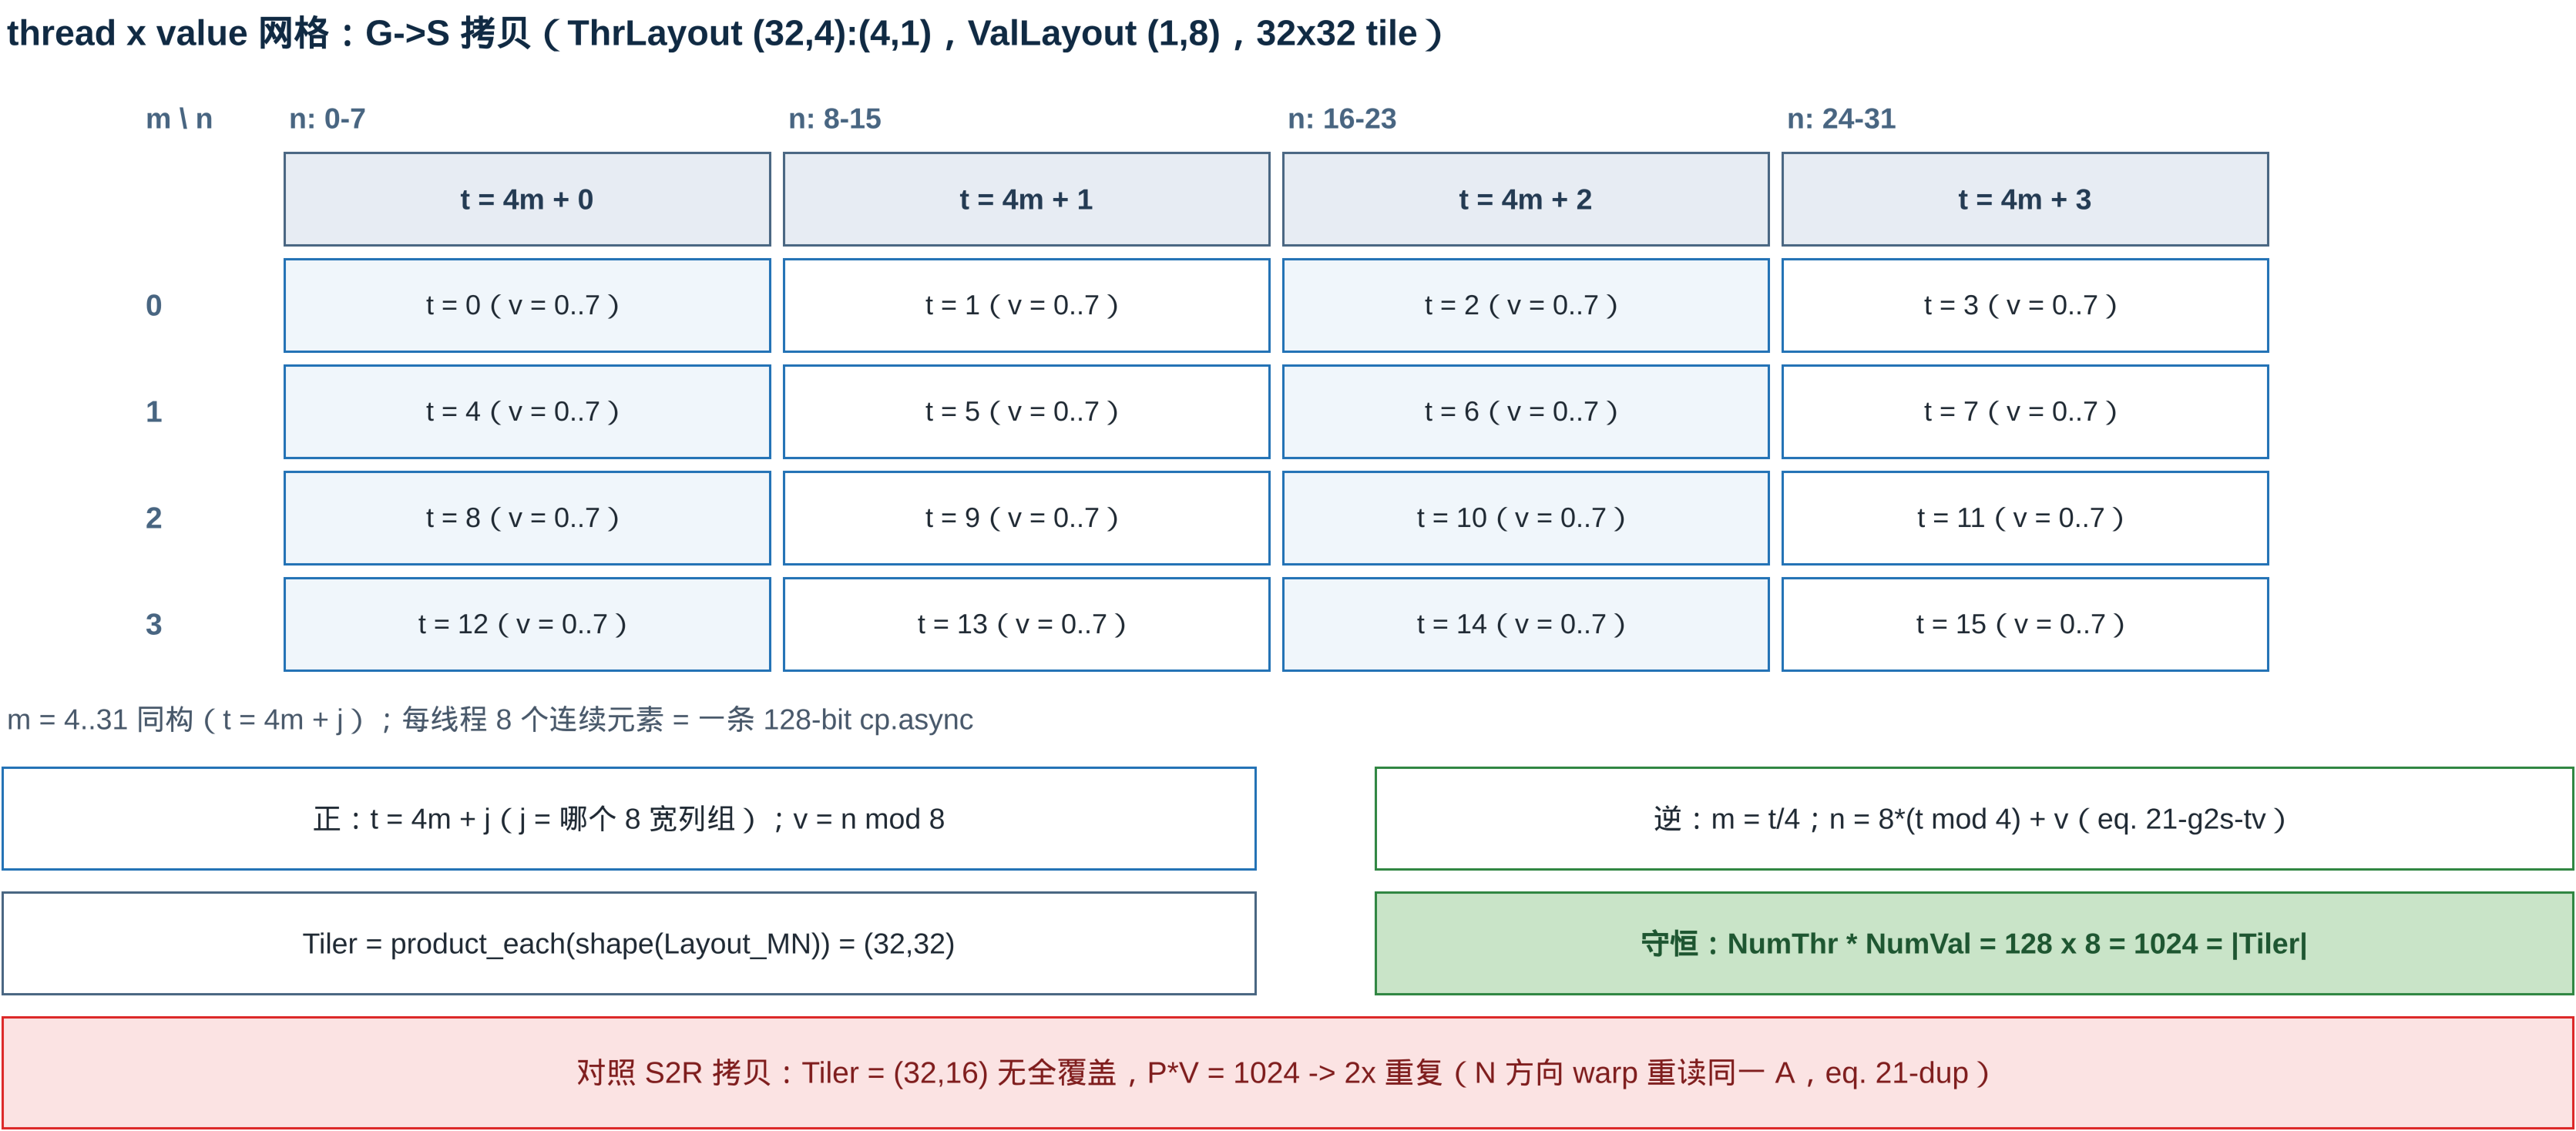
\includegraphics[width=0.95\textwidth]{figures/drawio/fig-21-3-g2s-grid/fig-21-3.png}
\begin{tikzpicture}[font=\tiny, x=0.015cm, y=-0.015cm]
  \node[anchor=west, font=\scriptsize\bfseries] at (24,26)
    {thread $\times$ value 网格：G$\to$S 拷贝（ThrLayout $(32,4){:}(4,1)$，
     ValLayout $(1,8)$，$32\times32$ tile）};
  \node[font=\tiny\bfseries] at (114,63) {$m \backslash n$};
  \foreach \cc/\nb in {0/{n: 0--7},1/{n: 8--15},2/{n: 16--23},3/{n: 24--31}}{
    \node[font=\tiny\bfseries] at ({251+216*\cc},63) {\nb};
    \ifcase\cc
      \def\chf{colorx4!12}%
    \or
      \def\chf{colorx4!24}%
    \or
      \def\chf{colorx4!36}%
    \else
      \def\chf{colorx4!48}%
    \fi
    \node[draw=colorx4!55, fill=\chf, font=\tiny\bfseries, minimum width=3.15cm,
          minimum height=0.6cm, inner sep=0pt] at ({251+216*\cc},98)
      {$t = 4m + \cc$};
  }
  \foreach \rr in {0,...,3}{
    \node[draw=gray!45, fill=white, minimum width=0.75cm, minimum height=0.36cm,
          inner sep=0pt] at (109,{144+46*\rr}) {$\rr$};
    \foreach \cc in {0,...,3}{
      \pgfmathtruncatemacro{\tn}{4*\rr+\cc}
      \ifcase\cc
        \def\cff{colorx4!12}%
      \or
        \def\cff{colorx4!24}%
      \or
        \def\cff{colorx4!36}%
      \else
        \def\cff{colorx4!48}%
      \fi
      \node[draw=colorx4!55, fill=\cff, minimum width=3.15cm, minimum height=0.6cm,
            inner sep=0pt] at ({251+216*\cc},{144+46*\rr})
          {$t = \tn$（$v = 0..7$）};
    }
  }
  \node[anchor=west, font=\tiny] at (24,323)
    {$m = 4..31$ 同构（$t = 4m + j$）；每线程 8 个连续元素 $=$ 一条 128-bit
     \texttt{cp.async}};
  \node[draw=tkBlue, fill=white, align=center, font=\tiny, text width=7.4cm,
        minimum height=0.66cm, inner sep=2pt] at (295,366)
    {正：$t = 4m + j$（$j =$ 哪个 8 宽列组）；$v = n \bmod 8$};
  \node[draw=tkGreen, fill=white, align=center, font=\tiny, text width=7.1cm,
        minimum height=0.66cm, inner sep=2pt] at (877,366)
    {逆：$m = t/4$；$n = 8(t \bmod 4) + v$（式~\eqref{eq:21-g2s-tv}）};
  \node[draw=gray!60, fill=white, align=center, font=\tiny, text width=7.4cm,
        minimum height=0.66cm, inner sep=2pt] at (295,420)
    {Tiler $=$ \texttt{product\_each(shape(Layout\_MN))} $= (32,32)$};
  \node[draw=tkGreen, fill=tkFillGreen, text=tkGreen!70!black, align=center,
        font=\tiny\bfseries, text width=7.1cm, minimum height=0.66cm, inner sep=2pt]
    at (877,420) {守恒：NumThr $\times$ NumVal $= 128 \times 8 = 1024 = |$Tiler$|$};
  \node[draw=tkRed, fill=tkFillRed, text=tkRed!80!black, align=center, font=\tiny,
        text width=16.0cm, minimum height=0.72cm, inner sep=2pt] at (580,476)
    {对照 S2R 拷贝：Tiler $= (32,16)$ 无全覆盖，$P\times V = 1024 \to 2\times$
     重复（N 方向 warp 重读同一 A，式~\eqref{eq:21-dup}）};
\end{tikzpicture}
\caption{thread$\times$value 网格：G$\to$S 拷贝把 $32\times32$ 的 tile 划成 $t=4m+j$ 的网格，每个线程搬 8 个连续元素（一条 128-bit \texttt{cp.async}）。同一划分用 MN 语言或 TV 语言描述是等价的（式~\eqref{eq:21-g2s-mn} 与式~\eqref{eq:21-g2s-tv}）。}
\label{fig:21-3}
\end{figure}

\begin{figure}[htbp]
\centering
% was: 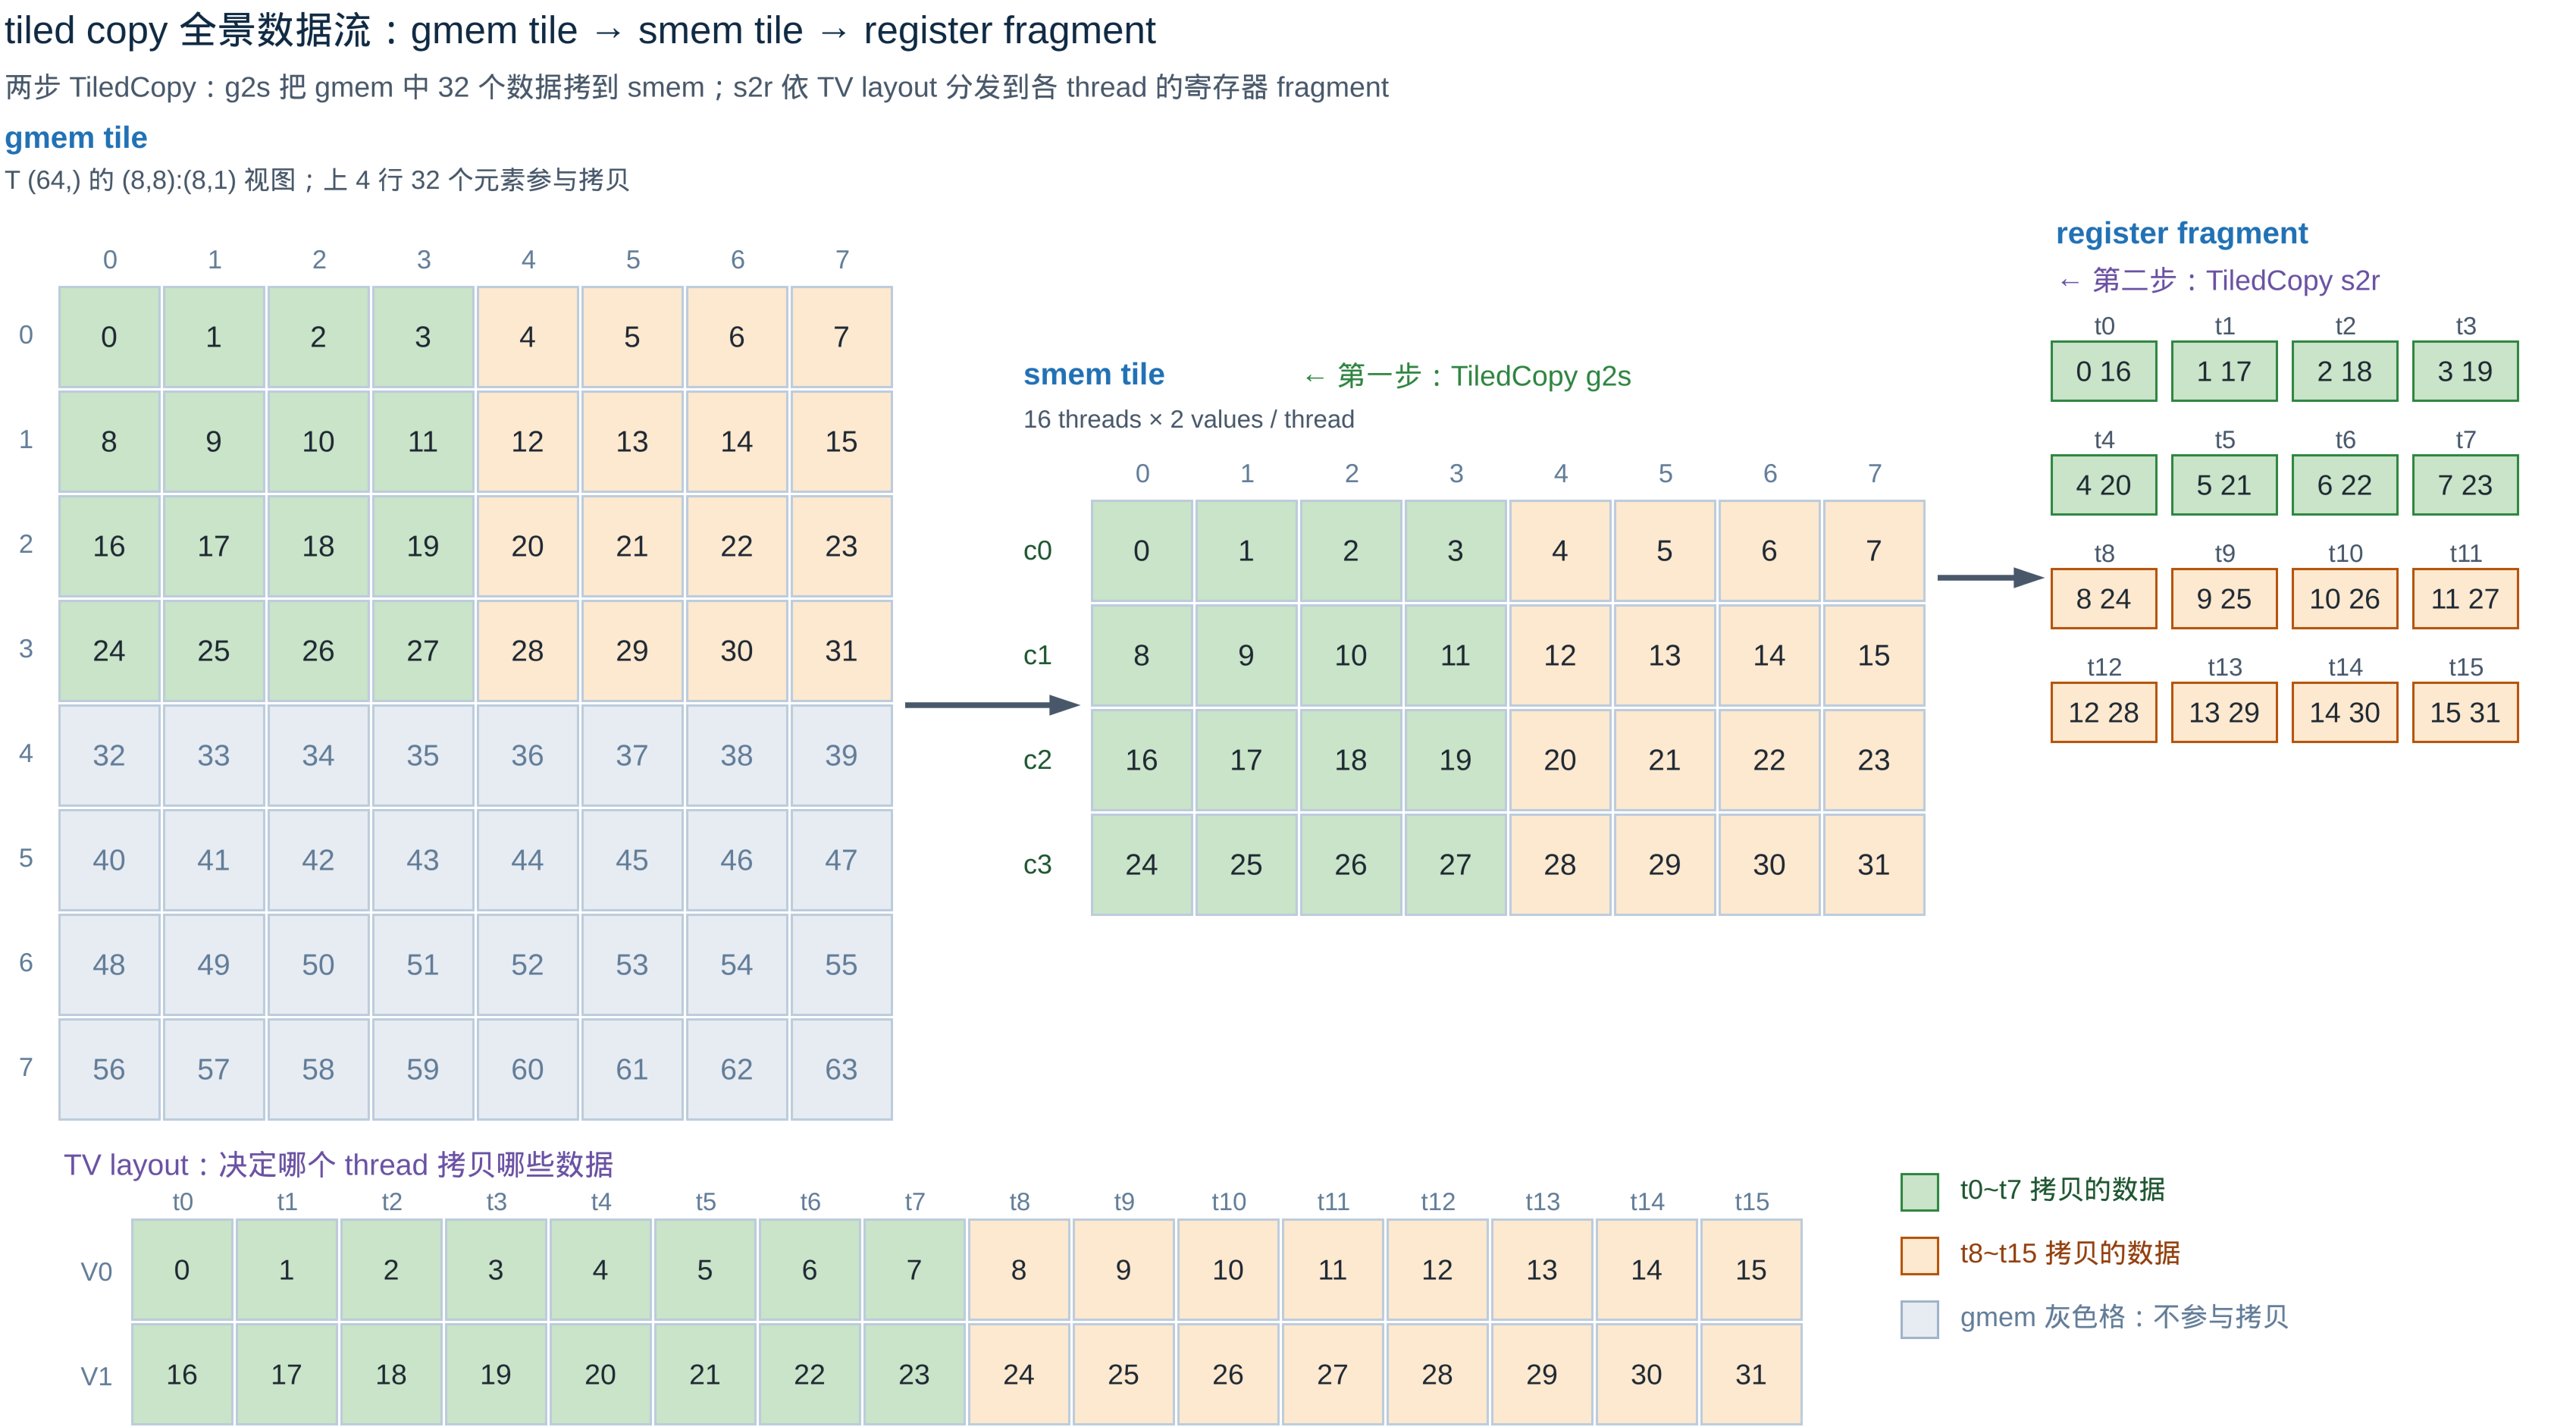
\includegraphics[width=0.95\textwidth]{figures/drawio/fig-21-4-tiled-copy-flow/fig-21-4.png}
\begin{tikzpicture}[font=\tiny, x=0.015cm, y=-0.015cm]
  \node[anchor=west, font=\footnotesize\bfseries] at (30,21)
    {tiled copy 全景数据流：gmem tile $\to$ smem tile $\to$ register fragment};
  \node[anchor=west, font=\tiny] at (30,46)
    {两步 TiledCopy：g2s 把 gmem 中 32 个数据拷到 smem；s2r 依 TV layout
     分发到各 thread 的寄存器 fragment};
  \node[anchor=west, font=\tiny\bfseries, text=tkBlue] at (30,68) {gmem tile};
  \node[anchor=west, font=\tiny] at (30,88)
    {$\mathrm{T}(64,)$ 的 $(8,8){:}(8,1)$ 视图；上 4 行 32 个元素参与拷贝};
  \foreach \cc in {0,...,7}{
    \node[font=\tiny, text=gray!80] at ({78+46*\cc},122) {\cc};
  }
  \foreach \rr in {0,...,7}{
    \node[anchor=east, font=\tiny, text=gray!80] at (50,{156+46*\rr}) {\rr};
    \foreach \cc in {0,...,7}{
      \pgfmathtruncatemacro{\vv}{8*\rr+\cc}
      \ifnum\rr>3
        \node[draw=gray!40, fill=gray!15, text=gray!90, minimum width=0.66cm,
              minimum height=0.66cm, inner sep=0pt] at ({78+46*\cc},{156+46*\rr}) {\vv};
      \else
        \ifnum\cc<4
          \node[draw=gray!40, fill=tkFillGreen, minimum width=0.66cm, minimum height=0.66cm,
                inner sep=0pt] at ({78+46*\cc},{156+46*\rr}) {\vv};
        \else
          \node[draw=gray!40, fill=tkFillOrange, minimum width=0.66cm, minimum height=0.66cm,
                inner sep=0pt] at ({78+46*\cc},{156+46*\rr}) {\vv};
        \fi
      \fi
    }
  }
  \node[anchor=west, font=\tiny\bfseries, text=tkBlue] at (478,172) {smem tile};
  \node[anchor=west, font=\tiny, text=tkGreen] at (600,173)
    {$\leftarrow$ 第一步：TiledCopy g2s};
  \node[anchor=west, font=\tiny] at (478,193) {16 threads $\times$ 2 values / thread};
  \foreach \cc in {0,...,7}{
    \node[font=\tiny, text=gray!80] at ({532+46*\cc},216) {\cc};
  }
  \foreach \rr in {0,...,3}{
    \node[anchor=east, font=\tiny, text=tkGreen!70!black] at (506,{250+46*\rr}) {c\rr};
    \foreach \cc in {0,...,7}{
      \pgfmathtruncatemacro{\vv}{8*\rr+\cc}
      \ifnum\cc<4
        \node[draw=gray!40, fill=tkFillGreen, minimum width=0.66cm, minimum height=0.66cm,
              inner sep=0pt] at ({532+46*\cc},{250+46*\rr}) {\vv};
      \else
        \node[draw=gray!40, fill=tkFillOrange, minimum width=0.66cm, minimum height=0.66cm,
              inner sep=0pt] at ({532+46*\cc},{250+46*\rr}) {\vv};
      \fi
    }
  }
  \node[anchor=west, font=\tiny\bfseries, text=tkBlue] at (932,110) {register fragment};
  \node[anchor=west, font=\tiny, text=tkPurple] at (932,131)
    {$\leftarrow$ 第二步：TiledCopy s2r};
  \foreach \rr in {0,...,3}{
    \foreach \cc in {0,...,3}{
      \pgfmathtruncatemacro{\vv}{4*\rr+\cc}
      \node[font=\tiny, text=gray!80] at ({955+53*\cc},{150+50*\rr}) {t\vv};
      \ifnum\rr<2
        \node[draw=tkGreen!60, fill=tkFillGreen, font=\tiny, minimum width=0.69cm,
              minimum height=0.39cm, inner sep=0pt] at ({955+53*\cc},{171+50*\rr})
          {\vv\ \ \the\numexpr\vv+16\relax};
      \else
        \node[draw=tkOrange!70, fill=tkFillOrange, font=\tiny, minimum width=0.69cm,
              minimum height=0.39cm, inner sep=0pt] at ({955+53*\cc},{171+50*\rr})
          {\vv\ \ \the\numexpr\vv+16\relax};
      \fi
    }
  }
  \node[anchor=west, font=\tiny, text=tkPurple] at (56,534)
    {TV layout：决定哪个 thread 拷贝哪些数据};
  \foreach \cc in {0,...,15}{
    \node[font=\tiny, text=gray!80] at ({110+46*\cc},552) {t\cc};
  }
  \foreach \rr in {0,1}{
    \node[anchor=east, font=\tiny, text=gray!80] at (84,{590+46*\rr}) {V\rr};
    \foreach \cc in {0,...,15}{
      \pgfmathtruncatemacro{\vv}{16*\rr+\cc}
      \ifnum\cc<8
        \node[draw=gray!40, fill=tkFillGreen, minimum width=0.66cm, minimum height=0.66cm,
              inner sep=0pt] at ({110+46*\cc},{590+46*\rr}) {\vv};
      \else
        \node[draw=gray!40, fill=tkFillOrange, minimum width=0.66cm, minimum height=0.66cm,
              inner sep=0pt] at ({110+46*\cc},{590+46*\rr}) {\vv};
      \fi
    }
  }
  \draw[-{Stealth[length=2mm]}, gray!70, very thick] (428,318) -- (502,318);
  \draw[-{Stealth[length=2mm]}, gray!70, very thick] (882,262) -- (926,262);
  \node[draw=tkGreen!60, fill=tkFillGreen, minimum width=0.24cm, minimum height=0.24cm,
        inner sep=0pt] at (874,532) {};
  \node[anchor=west, font=\tiny, text=tkGreen!70!black] at (890,532)
    {t0--t7 拷贝的数据};
  \node[draw=tkOrange!70, fill=tkFillOrange, minimum width=0.24cm, minimum height=0.24cm,
        inner sep=0pt] at (874,560) {};
  \node[anchor=west, font=\tiny, text=tkOrange!80!black] at (890,560)
    {t8--t15 拷贝的数据};
  \node[draw=gray!40, fill=gray!15, minimum width=0.24cm, minimum height=0.24cm,
        inner sep=0pt] at (874,588) {};
  \node[anchor=west, font=\tiny, text=gray!90] at (890,588) {gmem 灰色格：不参与拷贝};
\end{tikzpicture}
\caption{tiled copy 全景数据流：gmem tile（$(8,8)$ 视图，上半 32 个元素参与拷贝、下半灰色不参与）经 g2s TiledCopy 搬成连续 smem tile，再由 s2r 依 TV layout 切成每线程 fragment（thread $t$ 持 $\{t,\,t+16\}$ 两值）。两级 TiledCopy 的分工：g2s 把 strided 的全局块搬连续，s2r 按 thread$\times$value 分发到寄存器。重建自 @竹熙佳处《写给大家看的 CuTe 教程：tiled copy》。}
\label{fig:21-4}
\end{figure}

\section{性能分析}

本章没有独立的 kernel bench：TiledCopy 的开销无法单独测，它总是嵌在某个
kernel 的流水线里。所以本节回答的是这套抽象的开销构成，端到端数字留给
第~\ref{ch:24}~章（CuTe HGEMM 与手写版对照）。

\textbf{结论一（编译期零成本）}：Tiler、TV 布局、每个线程的地址全部是静态
类型推导的结果；kernel 里没有一行显式地址算术，\texttt{cute::copy} 内联后
就是 \texttt{cp.\allowbreak{}async.\allowbreak{}ca.\allowbreak{}shared.\allowbreak{}global} / \texttt{ldmatrix} / \texttt{st.shared}
的序列。第~\ref{ch:20}~章已经用 \texttt{static\_\allowbreak{}assert} 证明过同类折叠，本章
测试把 TiledCopy 的 Tiler/线程数/每线程值数也做成了静态断言。

\textbf{结论二（搬运划分影响访存质量）}：式~\eqref{eq:21-g2s-tv} 保证每个线程
的 8 个值连续，所以一个 128-bit Copy Atom 可以完成搬运。若把 Thr/Val 写错，
并不能指望 CuTe 自动把它降成 8 条 16-bit 访问：显式 Copy Atom 的
\texttt{copy\_unpack} 会尝试把输入重铸为原子访问类型，不满足布局和向量宽度
约束时会触发静态断言，错误配置也可能改变 tiler 与数据对应关系。正确做法是
先从 TV layout 核对每个 atom 的连续性和形状，再谈指令数量。

\textbf{结论三（epilogue 的额外成本）}：CuTe 版 epilogue 走
寄存器$\to$smem$\to$gmem 的 scratchpad 路线，比手写版的 shuffle $+$ 直接
wide store 多了两次 \texttt{\_\allowbreak{}\_\allowbreak{}syncthreads\allowbreak{}()}（每轮 R$\to$S 后与
S$\to$G 后各一次，L1116 与 L1184 附近）与一次 smem 往返。代价换来的是
\textbf{不写 shuffle 编排}：跨 lane 重组交给 sC 的布局做。对 $B_M\times B_N
=128\times256$ 的 tile，scratchpad 每轮搬 4 个 pipe slot（step $=4$），
R$\to$S/R$\to$G 各约 8 条指令，与主循环的 mma 数量相比是次要项，但它解释
了为什么 CuTe 版在极端配置下需要 \texttt{kSmemLayoutCBatch} 这类可调参数。

\textbf{结论四（重复因子放大的是 CTA 范围的副本数）}：式~\eqref{eq:21-dup} 的
A/B 重复因子为 $2$（hgemm 的 $2\times2$ warp 排布），表示不同 warp 需要
同一数据的寄存器副本，因而增加跨线程的覆盖点数和 CTA 总寄存器成本。它不是
每个线程的 fragment 元素数也乘上该因子；每线程仍按自己的
\texttt{partition\_\allowbreak{}fragment\_\allowbreak{}A/B} 持有固定数量的值。TiledCopy 只是
把这种跨线程重复原样体现在 partition 中。

\section{常见坑}

\textbf{坑一：\texttt{make\_\allowbreak{}tiled\_\allowbreak{}copy} 的 Thr/Val 是坐标 $\to$ 编号，
不是编号 $\to$ 坐标。}式~\eqref{eq:21-g2s-params} 的方向容易写反；
写成线程 $t$ 搬哪几个坐标的形式（即式~\eqref{eq:21-g2s-tv}）会得到形状
对、划分错的 TiledCopy：它不报错，只是每个线程搬了不连续的元素。

\textbf{坑二：\texttt{partition\_S}/\texttt{partition\_D} 的 S/D 不能用
gmem/smem 来记。}\allowbreak{}S 指 \emph{source side}、D 指 \emph{destination side}，
而每个 side 有自己的原子布局（\texttt{Val\allowbreak{}Layout\allowbreak{}Src}/\texttt{Val\allowbreak{}Layout\allowbreak{}Dst}）。
同一个 Tensor 既可能是 S 也可能是 D：\texttt{tAsA} 是 G$\to$S 的 D
（\texttt{partition\_\allowbreak{}D\allowbreak{}(s\allowbreak{}A)}），同时也是 S$\to$R 的 S
（\texttt{partition\_\allowbreak{}S\allowbreak{}(s\allowbreak{}A)}）。

\textbf{坑三：\texttt{retile} 不搬数据，也不能用来对齐线程。}
\texttt{retile\_D}/\texttt{retile\_S} 只重标索引，同一线程内的元素顺序被
重新解释；跨线程的重组必须靠 smem（或 shuffle）完成。写错方向的后果是
每个线程读到自己不该有的元素：数值错、不报错。

\textbf{坑四：动态 shape 会让 TV 布局退化。}
把 \texttt{Int<BM>} 换成运行期 \texttt{int}，\texttt{Tiler}、
\texttt{partition} 的形状都变成动态量，编译期折叠失效、地址算术回到运行期。
kernel 模板参数一律用 \texttt{Int<N>} 包住正是为此（第~\ref{ch:20}~章坑五的
同一件事，在 copy 上的表现）。

\textbf{坑五：\texttt{local\_tile} 之后仍带 remainder。}
\texttt{local\_\allowbreak{}tile\allowbreak{}(A,\allowbreak{} tile,\allowbreak{} coord)} 返回的 Tensor 仍带未切出的 mode
（gA 是三维的）；直接当二维用会在 \texttt{partition} 时报 rank 不匹配，
或者更隐蔽地，被 \texttt{\_} 占位符隐式丢掉一维。

\textbf{坑六：copy 的源/目的 shape 必须逐 mode 匹配。}
\texttt{cute::\allowbreak{}copy\allowbreak{}(tiled\_\allowbreak{}copy,\allowbreak{} src,\allowbreak{} dst)} 内部按元素对应，前提是
\texttt{src} 与 \texttt{dst} 的（值 $\times$ 剩余 mode）结构一致：这正是
\texttt{partition\_\allowbreak{}S\allowbreak{}(s\allowbreak{}A\_\allowbreak{}slice)} 与 \texttt{retile\_\allowbreak{}D\allowbreak{}(t\allowbreak{}Cr\allowbreak{}A)} 必须成对出现的
原因。只 partition 一侧、另一侧手写一个 shape 相近的 Tensor，会在
\texttt{copy} 内部的静态断言处编译失败（或者更糟，静默错位）。

\section{面试要点速查}

\textbf{Q1：CuTe 的 Tensor 是什么？为什么要与 layout 绑定？}\\
A：Tensor $=$ (Engine, Layout)，即一块内存 $+$ 一个坐标到 offset 的函数。
只有指针没有布局，就无法表达行主序/列主序/带 swizzle/切片后的视图；
绑定之后，切片、分区、拷贝都可以作为\emph{布局运算}在编译期完成。

\textbf{Q2：TV-layout 与 MN-layout 的关系？}\\
A：同一划分的两种视角，互为逆映射（式~\eqref{eq:21-mn-tv}）：MN 把坐标映到
(线程, 值)，TV 反过来。Tiler 由 MN 的 shape 取 product\_each 得到。

\textbf{Q3：\texttt{make\_\allowbreak{}tiled\_\allowbreak{}copy} 的 raked\_product 是什么意思？}\\
A：把 Thr/Val 两个坐标$\to$编号布局交错合成一个 MN 布局：同一线程的 $V$
个值沿坐标连续排布（raked $=$ 交错），而不是先按线程切大块。G$\to$S 的实例
就是式~\eqref{eq:21-g2s-mn}：$t=4m+\lfloor n/8\rfloor$、$v=n\bmod 8$。

\textbf{Q4：TiledCopy 的线程数 $\times$ 每线程值数一定等于 tile 大小吗？}\\
A：不一定。若 TV 布局是双射（G$\to$S、S$\to$G、C 类拷贝）则成立
（$128\times8=1024=32\times32$）；对 A/B 类拷贝会按 warp 排布出现重复因子
（式~\eqref{eq:21-dup}：A 的重复因子 $=$ N 方向 warp 数），因为多个 warp
需要同一份 fragment。

\textbf{Q5：\texttt{make\_\allowbreak{}tiled\_\allowbreak{}copy\_\allowbreak{}A/\allowbreak{}B/\allowbreak{}C} 从哪里得到线程映射？}\\
A：从 \texttt{TiledMMA} 的 \texttt{get\_\allowbreak{}layout\allowbreak{}A/\allowbreak{}B/\allowbreak{}C\_\allowbreak{}TV\allowbreak{}()} 直接取：MMA 的
fragment 约定已经规定了哪个线程持有哪个元素，拷贝只需把这份约定当作目的
布局（式~\eqref{eq:21-mtca}--\eqref{eq:21-mtcc}）。

\textbf{Q6：\texttt{retile\_S}/\texttt{retile\_D} 做了什么？}\\
A：零拷贝重标记：把 fragment 的（MMA, MMA\_M, MMA\_K）索引重排成 copy 视角的
（值, 重复）索引，\texttt{data()} 不变。它是 \texttt{copy} 逐元素对应的
前提，不做数据搬运、不做类型转换、不做 shuffle。

\textbf{Q7：\texttt{group\_modes} 与 \texttt{group} 的区别？}\\
A：\texttt{group<B,E>} 作用于 \emph{layout}，\texttt{group\_\allowbreak{}modes\allowbreak{}<B,\allowbreak{}E>} 作用于
\emph{Tensor}（内部就是前者）。合并 mode 只改索引结构，不改数据、不改物理地址。

\textbf{Q8：S$\to$R 的 K 方向为什么比 G$\to$S 多一层重复？}\\
A：原子不同。G$\to$S 的原子一次覆盖连续的 128-bit（8 half），而
\texttt{ldmatrix.x4} 一次只覆盖 $16\times16$ 的 K 切片；$B_K=32$ 时
G$\to$S 一个 tile 一级切完，S$\to$R 需要 2 个 K 切片（实测
\texttt{tAsA\_copy} 与 \texttt{tAsA} 的第三 mode 分别为 1 和 2）。

\section{最小测试与动手实验}

测试文件：\texttt{book/\allowbreak{}tests/\allowbreak{}ch21\_\allowbreak{}tiled\_\allowbreak{}copy.cu}（host-only：不启动 kernel、
不需要 GPU；只做类型/布局断言）。六个 case 覆盖本章全部可验证结论：

\begin{itemize}
  \item \textbf{A TV 分解}：G$\to$S 的 \texttt{TiledNumThr}$=128$、
        \texttt{TiledNumVal}$=8$、Tiler$=(32,32)$（编译期
        \texttt{static\_\allowbreak{}assert}），并对 1024 个 $(t,v)$ 对核对手推公式
        式~\eqref{eq:21-g2s-tv}（连同 3 条形状断言共 1027 checks）。
  \item \textbf{B partition 形状与守恒}：$(128,32)$ 上逐线程
        $(8,4,1)$、每线程 32 个元素、全部线程合计 4096；并把 4096 个
        (线程, 元素) 覆盖点映射回坐标，验证双射（\texttt{once}$=4096$）。
  \item \textbf{C fragment 与 retile}：TiledMMA（hgemm 配置）的
        \texttt{partition\_\allowbreak{}fragment\_\allowbreak{}A} 形状 $(8,4,2)$；
        \texttt{retile\_D} 后形状不变、\texttt{data()} 指针相同（零拷贝）。
  \item \textbf{D ldmatrix 的 source 视图}：S$\to$R 拷贝在 $(128,32)$ 上
        逐线程 64 个元素（$8\times4\times2$）、手推行/列公式逐点核对
        （线程 $t$ 的第 0 个值为 $\bigl(t\bmod 16 + 16\lfloor (t/32)\bmod
        2\rfloor,\ 8\lfloor (t\bmod 32)/16\rfloor\bigr)$；第 4 个线程模式
        步长为 0，即 $t$ 与 $t+64$ 同源）。
  \item \textbf{E 重复因子}：S$\to$R 的 A 拷贝对同一 tile 做覆盖统计，期望
        每个元素被覆盖恰好 2 次（N 方向 warp 的重复，式~\eqref{eq:21-dup}）。
  \item \textbf{F retile/upcast 语义}：\texttt{upcast} 式~\eqref{eq:21-upcast}
        两条；\texttt{upcast} 对 Swizzle 复合分配
        （\texttt{Sw\allowbreak{}<3,\allowbreak{}2,\allowbreak{}3>\ o \_\allowbreak{}0\ o\ \allowbreak{}(32,\allowbreak{}16):\allowbreak{}(16,\allowbreak{}1)}）；
        R$\to$S 拷贝的 tiler$(32,32)$、逐线程 $(8,1,1,4)$、单 pipe 覆盖
        1024 个坐标一次（双射）。
\end{itemize}

运行命令（在 \texttt{book/tests/} 下；脚本已配置 CUTLASS include 路径）：

\begin{lstlisting}[style=console]
cd kernels/interview/book/tests
CUDA_VISIBLE_DEVICES=6 ./build_tests.sh --arch sm_120a --ch ch21
\end{lstlisting}

预期输出（本机 RTX PRO 5000，CUDA 13.2，CUTLASS v4.6.1，2026-09-11 实测）：

\begin{lstlisting}[style=console]
ch21 CuTe Tensor & TiledCopy (host-only, no kernel launch)
PASS case A make_tiled_copy TV decomposition: mismatches=0 (1027 checks)
PASS case B partition_S shape & bijection: mismatches=0 (12544 checks)
PASS case C fragment shape & retile_D zero-copy: mismatches=0 (11 checks)
PASS case D ldmatrix source partitioning formula: mismatches=0 (16640 checks)
PASS case E A-copy duplication factor: mismatches=0 (3 checks)
PASS case F upcast semantics & R2S/S2G tilers: mismatches=0 (1814 checks)
ALL OK
\end{lstlisting}

动手实验（三条，都在本章测试上改）：

\begin{enumerate}
  \item 把 case~A 的 \texttt{ThrLayout} 从 $(32,4){:}(4,1)$ 改成
        $(4,32){:}(32,1)$（线程坐标 i/j 与 stride 一起换），观察
        \texttt{tv layout} 的公式断言如何失效，从而理解线程坐标的顺序与
        物理线程号的编号方式是两件事。
  \item 把 case~B 的源 Tensor 从 $(128,32)$ 换成 $(64,32)$，观察
        \texttt{partition\_S} 的剩余 mode 从 4 变 2、而每线程值数不变
        （8 个），并检查本轮覆盖统计是否有空洞。
  \item 把 case~C 的 \texttt{retile\_D} 换成 \texttt{retile\_S}，观察返回
        布局的形状差异，再对照 case~D 的 partition\_S 形状找出谁的形状该
        与谁相等的判据。
\end{enumerate}

\section*{延伸阅读}

\begin{itemize}
  \item @Anonymous《GEMM 细节分析(二)：TiledCopy 与 cp.async》，
        \url{https://zhuanlan.zhihu.com/p/703560147}
        （从 cp.async 的地址计算切入 TiledCopy 的划分，本章 3.4--3.6 节的
        对照读物）；
  \item @reed《cute 之 Copy 抽象》（Copy\_Atom/ThrCopy/partition
        抽象层次，4.2--4.4 节对照），
        \url{https://zhuanlan.zhihu.com/p/666232173}；
  \item @水木皇工仔《基于 CuTe 理解 swizzle, LDSM, MMA》，
        \url{https://zhuanlan.zhihu.com/p/934430036}
        （同一位作者把 LDSM 的 lane 映射与 MMA fragment 串起来讲，与本章
        case~D 的实验互补）；
  \item @竹熙佳处《写给大家看的 CuTe 教程：Tiled Copy》，
        \url{https://zhuanlan.zhihu.com/p/1930389542784964333}
        （本章 3.1--3.3 节的叙述框架参照该文：动机先行、小例子入手、
        表格视角；公式与实测以 CUTLASS v4.6.1 头文件为准）；
  \item @Anonymous《GEMM 细节分析(一)：ldmatrix 的选择》，
        \url{https://zhuanlan.zhihu.com/p/702818267}
        （ldmatrix 的转置/非转置选择，与第~\ref{ch:11}~章的手写版互证）。
\end{itemize}

% ch22-cute-tiledmma.tex — CuTe（三）：TiledMMA 与 fragment（RFC-F F3，2026-09-11）
% \url 由 book.tex 的 hyperref 提供；单章独立编译时降级为可断行的 \ttfamily
\makeatletter
\providecommand{\urlchbrk}[1]{\@tfor\next:=#1\do{\next\allowbreak}}
\makeatother
\providecommand{\url}[1]{{\ttfamily\urlchbrk{#1}}}
\chapter{CuTe（三）：TiledMMA 与 fragment}\label{ch:22}

\section{本章导读}

第~\ref{ch:21}~章把数据怎么搬形式化成了 TiledCopy；本章处理另一半：
计算怎么分给线程。一条 \texttt{mma.\allowbreak{}sync.\allowbreak{}aligned.\allowbreak{}m16n8k16} 是硬件
给出的最小计算单元，它规定了 32 个 lane 各自的 4（或 8）个寄存器里装哪几个
元素。而一个真实 kernel 的 tile 远大于 $16\times8\times16$，于是拿多个
MMA 原子去铺满 tile 需要一个统一的描述：这就是 \textbf{TiledMMA}：
原子 $\times$ 原子的排布 $\times$ 目标 tile 尺寸。

本章沿着第~\ref{ch:21}~章的 (thread, value) 语言继续：第~\ref{ch:21}~章里
TV 划分服务于\emph{搬运}，本章里 TV 划分服务于\emph{计算}，并且多出一个
维度：\textbf{fragment}（每个线程私有的寄存器数组）。核心问题是四个：
MMA 原子的 fragment 布局是什么（3.1 节）；TiledMMA 如何由原子 $+$ warp
排布 $+$ tile 尺寸构造出来（3.2 节）。partition 如何把 Tensor 切成
$(\mathrm{MMA}, \mathrm{MMA}_M, \mathrm{MMA}_K)$ 形状的片段
（3.3--3.5 节）；同一份寄存器为什么能在 QK 与 PV 两个不同的
TiledMMA 之间原地复用（4.3 节）。

\textbf{前置章节}：第~\ref{ch:20}~章（divide/zipped\_divide）、
第~\ref{ch:21}~章（Tensor 与 TV-layout）、第~\ref{ch:11}~章（m16n8k16 的
手写 fragment）、第~\ref{ch:15}~章（FA 的 P 复用背景）。\textbf{源码区间}：
ffpa\_attn.cuh~L31--64，即 \texttt{FFPAAttn\allowbreak{}Split\allowbreak{}DCu\allowbreak{}Te\allowbreak{}Traits} 的完整类型推导，
它是全书中唯一把\textbf{两个不同 tile 尺寸的 TiledMMA 写在同一个 traits 里}
的样本（QK 用 $64\times64\times16$ 一次覆盖 $S$，PV 用 $64\times16\times16$
控制累加器）。使用点引 ffpa\_attn.cuh~L151--158、L257--264、L300--305、
L339--345（cp.async 版本的 fragment 流转，与 TMA+WS 版逐行一致）。
\textbf{编译宏}：\texttt{NOTES\_\allowbreak{}V2\_\allowbreak{}ENABLE\_\allowbreak{}CUTE}。配套最小测试
\texttt{book/\allowbreak{}tests/\allowbreak{}ch22\_\allowbreak{}tiled\_\allowbreak{}mma.cu}：host 端 partition 一致性断言。

\section{问题与动机}

先从一条 mma 指令说起。\texttt{mma.\allowbreak{}sync.\allowbreak{}aligned.\allowbreak{}m16n8k16} 不是一个线程的
算术指令，而是一个 warp 的集体动作：32 个 lane 各自从自己的寄存器里
拿出 A、B 的一小片，硬件把它们拼成 $16\times16$ 与 $8\times16$ 的矩阵送进
tensor core。算完再把 $16\times8$ 的 C 分散写回 32 个 lane 的寄存器。所以
写 mma 的第一件事是回答我这条 lane 的寄存器里该装哪几个元素。
以 C（$16\times8$）为例，thread 0 负责 $(0,0)$、$(0,1)$、$(8,0)$、$(8,1)$
四个位置，thread 4 负责 $(1,0)$、$(1,1)$、$(9,0)$、$(9,1)$，以此类推
（@竹熙佳处《写给大家看的 CuTe 教程：tiled mma》把这张 thread-data 映射图
作为理解的起点）。

这些坐标是 PTX 规定的 fragment 布局，不是自由选择的。回忆第~\ref{ch:11}~章
手写 HGEMM 的寄存器清单：一条 m16n8k16 要 4 个 A 寄存器（8 个 half）、
2 个 B 寄存器（4 个 half）、4 个 C 寄存器（float）。以 A（$16\times16$，
列主序的 $(m,k)$）为例，lane 与元素的对应是

\begin{equation}
  \mathrm{row} = \Bigl\lfloor\frac{\mathrm{lane}}{4}\Bigr\rfloor,\qquad
  \mathrm{col} = 2\,(\mathrm{lane}\bmod 4) + (0\ \text{或}\ 1),
  \label{eq:22-ptx-a}
\end{equation}

外加 $+8$ 行与 $+8$ 列两套偏移把 8 个 half 填满。B（$8\times16$）的
对应关系类似。手写版（第~\ref{ch:11}~章）的做法是：把这些式子连同 ldmatrix
的 lane 地址表一起写在 kernel 里。这条路能走通，但三个问题随规模一起放大：

\begin{itemize}
  \item \textbf{换一条指令就要重查一次手册}。m16n8k8（fp16 半 K）、
        m16n8k32（int8）的 fragment 排布各不相同；每换一次，寄存器分配与
        地址算术都要重算，改对与否只能靠再跑一遍正确性测试；
  \item \textbf{跨架构可能要重写}。Volta 的 fragment 排布与 Ampere 不同，
        硬件换代意味着手推的公式作废：这是 CUDA $+$ PTX 路线的固有风险；
  \item \textbf{放大到 tile 级别没有参考模版}。真实 kernel 的 tile 远大于
        $16\times8\times16$：要么多起几个 warp 沿 M/N/K 排开（\emph{并行}
        维度），要么让一个 warp 循环执行多条 mma（\emph{串行}维度）。这两层
        重复的坐标运算（谁负责哪块、重复多少次、寄存器怎么编号），
        手推起来极易出错。
\end{itemize}

CuTe 对这三处问题的回应可以概括为：把 atom 的 thread-data 映射本身变成
一个 layout，然后让重复成为 layout 的乘法。

把上述规则放到 FFPA 上实例化。FFPA 的 QK 步骤要算
$S_{64\times64} = Q_{64\times64} K^T_{64\times64}$（每个 d-chunk），PV 步骤
要算 $O_{64\times64} = P_{64\times64} V_{64\times64}$，即两个 $64\times64$ 的
结果，每个线程要用多条 m16n8k16 拼出来。拼的规则至少包括：

\begin{itemize}
  \item \textbf{warp 怎么分}：QK 用 4 个 warp 沿 M 方向切（每个 warp 16 行），
        还是 $2\times2$ 网格？不同选择决定 A/B fragment 的重复因子
        （第~\ref{ch:21}~章式~(21-dup)）。
  \item \textbf{每个 warp 内部怎么重复}：一个 warp 覆盖 16 行 $\times$ 64 列时，
        N 方向要 8 个原子；这 8 个原子的寄存器块怎么编号。
  \item \textbf{K 方向怎么切}：tile 的 K 长度是 64，而原子是 16，于是 fragment
        多出一个 $\mathrm{MMA}_K$ mode。
  \item \textbf{两个不同形状的 tile 怎么并存}：QK 要大 tile（省循环、提高
        计算密度），PV 要小 N tile（控制 per-call 视图与临时开销），它们
        必须共享同一套线程/值编号。
\end{itemize}

CuTe 的答案是把这四件事收进一个类型：\texttt{Tiled\allowbreak{}MMA\allowbreak{}<MMA\_\allowbreak{}Atom,\allowbreak{}
Atom\allowbreak{}Layout\allowbreak{}MNK,\allowbreak{} Permutation\allowbreak{}MNK>}。一个 TiledMMA 实例只回答两个问题：
这个 tile 有哪些 (线程, 值) 位置；给定一个 Tensor 时，
每个线程的 fragment 是什么形状。@竹熙佳处把动机总结成\textbf{给定任意一条
mma 指令，都能方便地推导出每个线程该从 data tile 里取哪一部分}，与这里的
两个问题是同一件事的两种说法。本章要验证的，就是这两个回答在 FFPA 的
具体配置下能否用手推公式复现，不能复现就说明没读懂。

\section{数学原理}

\subsection{MMA 原子：一条指令的 thread-data 映射}

最小尺度是一条指令、一个 warp。C 的 thread 0 拿 $(0,0)$、$(0,1)$、
$(8,0)$、$(8,1)$，thread 4 拿 $(1,0)$、$(1,1)$、$(9,0)$、$(9,1)$。这张
thread-data 对照表就是原子的全部内容。CuTe 用一个 traits 类把它写成类型
（\texttt{MMA\_\allowbreak{}Traits\allowbreak{}<Op>}），FFPA 用到的
\texttt{SM80\_\allowbreak{}16x8x16\_\allowbreak{}F32\allowbreak{}F16\allowbreak{}F16\allowbreak{}F32\_\allowbreak{}TN} 实测（CUTLASS v4.6.1）为：

\begin{center}
\footnotesize
\begin{tabular}{@{}lll@{}}
  \toprule
  成员 & 值 & 含义 \\
  \midrule
  \texttt{Shape\_MNK} & $(16,8,16)$ & 原子覆盖的 $M\times N\times K$ \\
  \texttt{ThrID} & $\mathrm{Layout}\_32$ & 原子用 32 个线程（一个 warp） \\
  \texttt{LayoutA\_TV} & $((4,8),(2,2,2)){:}((32,1),(16,8,128))$ & $(\mathrm{thr},\mathrm{val})\to$ A 的扁平坐标 \\
  \texttt{LayoutB\_TV} & $((4,8),(2,2)){:}((16,1),(8,64))$ & $(\mathrm{thr},\mathrm{val})\to$ B 的扁平坐标 \\
  \texttt{LayoutC\_TV} & $((4,8),(2,2)){:}((32,1),(16,8))$ & $(\mathrm{thr},\mathrm{val})\to$ C 的扁平坐标 \\
  \bottomrule
\end{tabular}
\end{center}

这些 layout 的 codomain 是\textbf{扁平坐标}：A 的扁平量是 $m + 16k$（M 最快），
B 是 $n + 8k$，C 是 $m + 16n$，三者都按第一个 mode 最快的 colex 约定
（第~\ref{ch:20}~章式~(20-colex-decomp)）线性化。于是三份
\texttt{Layout*\_TV} 就是 thread-data 映射的类型化写法：
给它一个 (lane, 值编号)，它返回该元素在原子小矩阵里的扁平坐标。
以 \texttt{LayoutC\_TV} $=((4,8),(2,2)){:}((32,1),(16,8))$ 为例，用映射
语言说：lane 被拆成 $(\mathrm{lane}\bmod4,\ \lfloor\mathrm{lane}/4\rfloor)$
两维，低位那维的 stride 是 $32$，因为 C 的扁平坐标按 $m+16n$ 线性化，
$32$ 恰好是\emph{两列}（列号加 2），高位那维 stride 是 $1$（行号加 1）；
值编号的两维 stride 为 $16$（列加 1）与 $8$（行加 8，即装填用的 $+8$ 行
偏移）。把 stride 反解回坐标，就得到三条可以独立验证的公式
（lane $=\mathrm{thr}$，值编号 $v$ 按 colex 拆位）：

\begin{align}
  \textbf{A}:\quad &m = \Bigl\lfloor\frac{\mathrm{lane}}{4}\Bigr\rfloor + 8\,d_1,
  \quad k = 2\,(\mathrm{lane}\bmod 4) + d_0 + 8\,d_2, \label{eq:22-atom-a}\\
  \textbf{B}:\quad &n = \Bigl\lfloor\frac{\mathrm{lane}}{4}\Bigr\rfloor,
  \quad k = 2\,(\mathrm{lane}\bmod 4) + d_0 + 8\,d_1, \label{eq:22-atom-b}\\
  \textbf{C}:\quad &m = \Bigl\lfloor\frac{\mathrm{lane}}{4}\Bigr\rfloor + 8\,d_1,
  \quad n = 2\,(\mathrm{lane}\bmod 4) + d_0, \label{eq:22-atom-c}
\end{align}

其中 $(d_0,d_1,d_2)$ 是值编号 $v$ 在原子值 mode 上的 colex 分解
（A：$v=d_0+2d_1+4d_2$，8 个 half；B/C：$v=d_0+2d_1$，4 个元素）。
式~\eqref{eq:22-atom-a}--\eqref{eq:22-atom-c} 与 PTX 文档给的 m16n8k16
fragment 图完全一致。

例如 lane 0 的 A 是
\begin{equation*}
  \{(0,0),(0,1),(8,0),(8,1),(0,8),(0,9),(8,8),(8,9)\},
\end{equation*}
lane 31 是 $\{(7,6),(7,7),(15,6),(15,7),(7,14),\dots\}$。CuTe 没有
另立一套约定，它就是 PTX 约定的类型化表达。本章测试 case~A 对三条公式在
32 个 lane 上逐点核对，并用 32 线程 $\times$ 每线程值数 $=$ 原子元素数
验证守恒（A：$32\times8=256=16\times16$；B：$32\times4=128=8\times16$；
C：$32\times4=128=16\times8$）。

单 warp 演练：\texttt{partition\_\allowbreak{}fragment\_\allowbreak{}A/\allowbreak{}B/\allowbreak{}C} 给出什么？
把原子包成最小的 TiledMMA（warp 排布 $(1,1,1)$，tile 参数就是原子形状），
对一个 $16\times16$ 的 A、$8\times16$ 的 B、$16\times8$ 的 C 调用三个
partition：tile 不放大、线程不增，每线程拿到的就是原子自身的一份 fragment：
A 为 $(8,1,1)$（8 个 half）、B 为 $(4,1,1)$、C 为 $(4,1,1)$，与
第~\ref{ch:11}~章手写版的寄存器清单逐一对应。partition
在单 warp $+$ 单原子的退化情形下输出的就是 PTX fragment 本身；它真正的
价值（tile 放大后的 remainder 与多 warp 的重复因子）要到 3.2--3.3 节才
显现。

\subsection{TiledMMA：原子、排布、tile 三个参数}

动机里那两层重复是并行维度（多起执行器）与串行维度（一个执行器循环执行）。
CuTe 把两者装进
\texttt{make\_\allowbreak{}tiled\_\allowbreak{}mma\allowbreak{}(atom,\allowbreak{} Atom\allowbreak{}Layout\allowbreak{}MNK,\allowbreak{} Permutation\allowbreak{}MNK)} 的三个参数：
原子是硬件粒度，第二个参数是 warp 排布（哪个 warp 覆盖哪个原子位置，
负责并行重复），第三个是目标 tile 尺寸（含 K，决定一个 threadblock
一次执行的计算块）。内核把两者合成为

\begin{equation}
  \mathrm{ThrLayoutVMNK} = \mathrm{tiled\_product}(\mathrm{ThrID},\
  \mathrm{AtomLayoutMNK}) \ \cong\ (\mathrm{ThrV},\mathrm{ThrM},
  \mathrm{ThrN},\mathrm{ThrK}) ,
  \label{eq:22-thr-vmnk}
\end{equation}

实测（FFPA 的 QK）：
$\mathrm{thr\_layout\_vmnk} = (32,4,1,1){:}(1,32,0,0)$，$\mathrm{ThrV}=32$
是 warp 内部线程（stride 1），$\mathrm{ThrM}=4$ 是 4 个 warp 沿 M 排列
（stride 32）。同时 tile 的尺寸由

\begin{equation}
  \mathrm{tile\_size}_I = \mathrm{size}\bigl(\mathrm{permutation\_mnk}\langle I\rangle\bigr),
  \qquad
  \mathrm{permutation\_mnk}\langle I\rangle =
  \begin{cases}
    \text{显式给定}, & \text{非下划线},\\[2pt]
    \mathrm{atom}_I \times \mathrm{Thr}_I, & \text{否则},
  \end{cases}
  \label{eq:22-tile-size}
\end{equation}

给出：QK 实测 $\mathrm{tile\_size} = (64,64,16)$，PV 为 $(64,16,16)$
（FFPA 两者都显式给定）。式~\eqref{eq:22-tile-size} 的第二行是不显式
给时的算法：$\mathrm{tile}_I = \mathrm{atom}_I \times \mathrm{Thr}_I$，
原子长度乘该方向的 warp 组数（M 对应
$\mathrm{ThrM}$、N 对应 $\mathrm{ThrN}$、K 对应 $\mathrm{ThrK}$）。

用映射语言说：\texttt{Thr\allowbreak{}Layout\allowbreak{}VMNK} 把线程编号拆成
$(\mathrm{ThrV},(\mathrm{ThrM},\mathrm{ThrN},\mathrm{ThrK}))$ 四层：先分
warp 内部（$\mathrm{ThrV}$），再分第几个 warp 落在哪个方向。
谁并行、谁重复这两个问题的答案，都由线程编号到 VMNK 的分解给出。

一个自然的疑问是：既然 warp 排布 $+$ 原子尺寸已经能划分 tile，为什么还要
第三个（tile）参数？@竹熙佳处给出两条理由。

一是拷贝粒度：后续 S2R/R2S tiled copy 把这个参数描述的块整体当作拷贝单位，
N 方向留大一倍（每个 warp 16 而非 8）才能用上 \texttt{ldsm.x4} 一类的
宽指令。二是重排的余地：tile 参数本质是一个 layout，高级用法可以借助它的
stride 把多条指令算出的数据在寄存器里重新排列，
\texttt{Permutation\allowbreak{}MNK} 这个名字就来自这里。常规场景把它当 tile 尺寸读即可。

\subsection{q 的推导链：从 tile 到 fragment}

真正的工作在 \texttt{thrfrg\_\allowbreak{}A/\allowbreak{}B/\allowbreak{}C} 里，它是四步 layout 代数
（第~\ref{ch:20}~章的全部工具在这里综合使用）。四步走的是一条固定流水线：
先按 tile 切、再按原子切、把原子坐标换成 (线程, 值)、最后按 warp
排布把线程剥出来。以 A 为例（B/C 只是把 mode 换成 $(N,K)$ / $(M,N)$）：

\begin{align}
  &\text{(1) 按 tile 分块} &
  T_1 &= \mathrm{logical\_divide}\bigl(A,\!(\mathrm{perm}_M, \mathrm{perm}_K)\bigr),
  \label{eq:22-thrfrg-1}\\
  &\text{(2) 按原子切分} &
  T_2 &= \mathrm{zipped\_divide}\bigl(T_1,\ (\mathrm{atom}_M,
  \mathrm{atom}_K)\bigr) = \bigl((A_M,A_K),(R_M,R_K)\bigr),
  \label{eq:22-thrfrg-2}\\
  &\text{(3) 原子坐标}\!\to\!(\text{线程},\text{值}) &
  T_3 &= T_2 \circ \mathrm{LayoutA\_TV} = \bigl((\mathrm{ThrV},
  \mathrm{FrgV}),(R_M,R_K)\bigr),
  \label{eq:22-thrfrg-3}\\
  &\text{(4) 按 warp 排布切分} &
  T_4 &= \mathrm{zipped\_divide}\bigl(T_3, (\_,
  (\mathrm{ThrM},\mathrm{ThrK}))\bigr) \notag\\
  & & &= \bigl((\mathrm{ThrV},
  (\mathrm{ThrM},\mathrm{ThrK})),(\mathrm{FrgV}, (R'_M, R'_K))\bigr).
  \label{eq:22-thrfrg-4}
\end{align}

概括这条链：把 tensor 按坐标层层切开，切到只剩原子的 MN
坐标，再经 \texttt{LayoutA\_TV} 换成 (线程, 值)。四步里的三个量各司其职：
第 (1) 步的 $\mathrm{perm}$ 决定一个 tile 多大，第 (2) 步的
$\mathrm{atom}$ 决定一条指令多大，第 (4) 步的
$\mathrm{ThrM/ThrK}$ 决定多少 warp 分摊，正是 3.2 节三个参数的第三次
出现。对线程 $t$ 来说，前三步的结果对所有线程相同，只有第 (4) 步把该线程
自己区分出来。

把第 (4) 步的线程坐标 $(\mathrm{ThrV},\mathrm{ThrM},\mathrm{ThrK})$ 用
\texttt{get\_\allowbreak{}slice\allowbreak{}(t)} 固定住，剩下的就是该线程的 fragment 形状：

\begin{equation}
  \mathrm{fragment} = \bigl(\underbrace{\mathrm{FrgV}}_{\mathrm{MMA}},\
  \underbrace{R'_M}_{\mathrm{MMA}_M},\ \underbrace{R'_K}_{\mathrm{MMA}_K}\bigr) ,
  \label{eq:22-fragment}
\end{equation}

$R'_M = R_M/\mathrm{ThrM}$、$R'_K = R_K/\mathrm{ThrK}$ 是 warp 分完之后每个
线程还要重复多少个原子。以 FFPA 的 QK（tile $64\times64\times16$、
$\mathrm{AtomLayout}=(4,1,1)$）在 $64\times64$ 的 Q 上为例逐项算：

\begin{itemize}
  \item (1)  $\mathrm{perm} = (64,16)$：$T_1 = ((64,16),(1,4))$；
  \item (2)  $\mathrm{atom}=(16,16)$：$T_2 = ((16,16),(4,4))$，即
        $R_M = 64/16 = 4$、$R_K = 64/16 = 4$；
  \item (3)  $\mathrm{LayoutA\_TV}$ 把 $(16,16)$ 变成 $(\mathrm{ThrV}=32,
        \mathrm{FrgV}=8)$：$T_3 = ((32,8),(4,4))$；
  \item (4)  $\mathrm{ThrM}=4$：$(\mathrm{FrgV},(R'_M,R'_K)) = (8,(1,4))$。
\end{itemize}

于是 $\mathrm{MMA}=8$、$\mathrm{MMA}_M = 1$、$\mathrm{MMA}_K = 4$，
fragment 大小 $8\times1\times4 = 32$，与本章测试 case~C 的实测
\texttt{\allowbreak{}(\allowbreak{}(2,\allowbreak{}2,\allowbreak{}2),\allowbreak{}1,\allowbreak{}4)} 完全一致（$(2,2,2)$ 是 8 的嵌套写法）。
测试同时对 B 与 C 复算了这条链：QK 的 B 在 $(64,64)$ 上得
$(4,8,4)$（$=128$ 个 half/线程，因为 4 个 M-warp 各持一份完整 B，重复因子 4，
式~\eqref{eq:22-dup}）；C 得 $(4,1,8) = 32$（无重复，$4096/128$）。四步
推导链的 shape 演化见图~\ref{fig:22-thrfrg-chain}。

\begin{figure}[H]
\centering
\begin{tikzpicture}[font=\tiny]
  \begin{scope}
    \foreach \fk in {0,...,3}{
      \ifnum\fk=0 \def\cfill{colorx4!40} \else \def\cfill{gray!22} \fi
      \fill[\cfill] ({0.6*\fk},0) rectangle ({0.6*\fk+0.6},{-2.4});
    }
    \draw[thin] (0,0) grid[xstep=0.6cm, ystep=0.3cm] (2.4,-2.4);
    \draw[very thick] (0,0) rectangle (2.4,-2.4);
    \node[font=\tiny, rotate=90] at (0.3,-1.2) {tile $(64,16)$};
    \node[font=\tiny, rotate=90] at (1.5,-1.2) {rest $(1,4)$：4 个 K 切片};
    \node[anchor=south, font=\tiny] at (1.2,0.48) {$A$：$64\times64$，perm $=(64,16)$};
    \node[anchor=south, font=\tiny\bfseries] at (1.2,0.11) {(1) logical\_divide};
    \node[anchor=north, font=\tiny] at (1.2,-2.55) {$T_1=((64,16),(1,4))$};
  \end{scope}
  \draw[->, very thick] (2.6,-1.2) -- (3.3,-1.2);
  \begin{scope}[shift={(3.5,0)}]
    \foreach \am in {0,...,3}{
      \foreach \ak in {0,...,3}{
        \pgfmathtruncatemacro{\pk}{mod(\am+\ak,2)}
        \ifnum\pk=0 \def\cfill{colorx4!15} \else \def\cfill{colorx6!40} \fi
        \fill[\cfill] ({0.33*\ak},{-0.6*\am}) rectangle ({0.33*\ak+0.33},{-0.6*\am-0.6});
      }
    }
    \draw[thin] (0,0) grid[xstep=0.33cm, ystep=0.6cm] (1.32,-2.4);
    \draw[very thick] (0,0) rectangle (1.32,-2.4);
    \node[anchor=south, font=\tiny] at (0.66,0.48) {atom $(16,16)$};
    \node[anchor=south, font=\tiny\bfseries] at (0.66,0.11) {(2) zipped\_divide};
    \node[anchor=north, font=\tiny, align=center] at (0.66,-2.55)
      {$T_2=((16,16),(4,4))$，$R_M{=}R_K{=}4$\\（棋盘 $=$ atom 身份）};
  \end{scope}
  \draw[->, very thick] (5.0,-1.2) -- (5.4,-1.2);
  \begin{scope}[shift={(5.6,0)}]
    \foreach \gm/\gk in {0/0,0/1,0/8,0/9,8/0,8/1,8/8,8/9}{
      \fill[colorx1!50] ({0.135*\gk},{-0.135*\gm}) rectangle ({0.135*\gk+0.135},{-0.135*\gm-0.135});
    }
    \draw[thin] (0,0) grid[xstep=0.135cm, ystep=0.135cm] (2.16,-2.16);
    \draw[very thick] (0,0) rectangle (2.16,-2.16);
    \node[anchor=south, font=\tiny, align=center] at (1.08,0.44) {atom $(16,16)\to$\\$(\mathrm{thr},\mathrm{val})$};
    \node[anchor=south, font=\tiny\bfseries] at (1.08,0.11) {(3) $\circ$ LayoutA\_TV};
    \node[anchor=north west, font=\tiny, align=left] at (5.75,-2.52)
      {深色 8 格 $=$ lane 0 的 FrgV：$\{(0,0),(0,1),(8,0),(8,1),$\\
       $(0,8),(0,9),(8,8),(8,9)\}$（式~\eqref{eq:22-atom-a}）};
    \node[anchor=north, font=\tiny] at (1.08,-3.32) {$T_3=((32,8),(4,4))$};
  \end{scope}
  \draw[->, very thick] (7.95,-1.2) -- (8.4,-1.2);
  \begin{scope}[shift={(8.6,0)}]
    \foreach \am in {0,...,3}{
      \foreach \ak in {0,...,3}{
        \ifnum\am=1 \def\cfill{colorx3!45} \else \def\cfill{gray!22} \fi
        \fill[\cfill] ({0.33*\ak},{-0.6*\am}) rectangle ({0.33*\ak+0.33},{-0.6*\am-0.6});
      }
    }
    \draw[thin] (0,0) grid[xstep=0.33cm, ystep=0.6cm] (1.32,-2.4);
    \draw[very thick] (0,0) rectangle (1.32,-2.4);
    \draw[thick] (0,-0.6) -- (1.32,-0.6);
    \draw[thick] (0,-1.2) -- (1.32,-1.2);
    \draw[thick] (0,-1.8) -- (1.32,-1.8);
    \draw[->, thick] (1.5,-0.9) -- (1.36,-0.9);
    \node[anchor=west, font=\tiny, align=left] at (1.56,-0.9)
      {warp $w$（thrM $=w$）的行带；\\get\_slice$(t)$ 后 $R'_M{=}1$、$R'_K{=}4$};
    \node[anchor=south, font=\tiny] at (0.66,0.48) {$(\_,(\mathrm{ThrM},\mathrm{ThrK}))=(4,1)$};
    \node[anchor=south, font=\tiny\bfseries] at (0.66,0.11) {(4) zipped\_divide};
    \foreach \ak in {0,...,3}{
      \ifcase\ak
        \def\cff{colorx4!15}%
      \or
        \def\cff{colorx4!30}%
      \or
        \def\cff{colorx4!45}%
      \else
        \def\cff{colorx4!60}%
      \fi
      \draw[fill=\cff, thick] ({0.33*\ak},-3.35) rectangle ({0.33*\ak+0.33},-3.05);
      \node[font=\tiny] at ({0.33*\ak+0.165},-3.2) {8};
    }
    \node[anchor=east, font=\tiny] at (-0.1,-3.2) {FrgV};
    \node[anchor=north, font=\tiny, align=center] at (0.66,-3.5)
      {$(\mathrm{FrgV},(R'_M,R'_K))=(8,(1,4))$\\$\mathrm{MMA}_K{=}4$ 个 atom $\times$ 每原子 8 half};
  \end{scope}
  \node[anchor=north west, font=\tiny, align=left] at (0,-4.35)
    {fragment $=(\mathrm{MMA},\mathrm{MMA}_M,\mathrm{MMA}_K)=(8,1,4)$：每线程
     $8\times1\times4=32$ half；\\ $\times\,128$ 线程 $=4096=64\times64$
     （双射，case~C/D）；\\ B/C 同链只换 mode：B 得 $(4,8,4)$（4 倍重复）、
     C 得 $(4,1,8)$。};
\end{tikzpicture}
\caption{thrfrg\_A 四步推导链（式~\eqref{eq:22-thrfrg-1}--\eqref{eq:22-thrfrg-4}）
在 FFPA QK（tile $64\times64\times16$、AtomLayout $(4,1,1)$、Q 为
$64\times64$）上的 shape 演化：(1) logical\_divide 按 tile 切出 $(64,16)$
与 4 个 K 切片；(2) zipped\_divide 按 atom $(16,16)$ 切成 $4\times4$ 个
原子块；(3) 复合 LayoutA\_TV 把原子内坐标换成（线程, 值），深色 8 格即
lane 0 的 FrgV；(4) 按 $(\mathrm{ThrM},\mathrm{ThrK})=(4,1)$ 剥出 warp 行带，
get\_slice$(t)$ 后每线程 fragment $=(8,(1,4))=32$ half（右下：FrgV $=8$
$\times$ $\mathrm{MMA}_K=4$）。}
\label{fig:22-thrfrg-chain}
\end{figure}

\begin{equation}
  \text{A 的重复因子} = \#\{\text{N-warp}\},\qquad
  \text{B 的重复因子} = \#\{\text{M-warp}\},\qquad
  \text{C 无重复} .
  \label{eq:22-dup}
\end{equation}

\subsection{守恒与 tile 循环}

把三个 fragment 的每线程元素数乘以线程数，得到的是数据被读了几遍：
C 恰好等于 tile 元素数（$128\times32 = 4096 = 64\times64$，双射），
A 也是（$\mathrm{ThrK}=1$ 时无 K-warp 重复），B 是 4 倍。这个重复因子在选 tile 时
必须算清楚：B 的 4 倍重复意味着 128 个 half/线程的寄存器开销，它不占
smem，但占用寄存器预算。守恒式也是最便宜的自检：两边对不上，说明有数据没有
线程负责、或有线程在空转（本章测试 case D 就是这条守恒式的逐点版本）。

当 tensor 比 tile 大时，partition 会多出 tile 重复 mode：$64\times64$ 的
tile 作用在 $64\times256$ 的 C 上，$\mathrm{MMA}_N$ 从 8 变成 32。这不是新
机制，只是式~\eqref{eq:22-thrfrg-1} 的 $T_1$ 多留了一层 remainder。
\texttt{gemm\allowbreak{}(tiled\_\allowbreak{}mma,\allowbreak{} A,\allowbreak{} B,\allowbreak{} C)} 会在这一层 remainder 上循环，这正是
第~\ref{ch:21}~章 kernel 里只显式展开 K 循环、M/N 交给 \texttt{cute::gemm}
的原因（hgemm.cuh~L925--937 的注释）。

\subsection{get\_slice：线程坐标的三层解构}

一行调用 \texttt{thr\_\allowbreak{}mma =\allowbreak{} tiled\_\allowbreak{}mma.\allowbreak{}get\_\allowbreak{}slice\allowbreak{}(t)} 就能完成线程坐标的
三层解构：把整数 $t$ 按式~\eqref{eq:22-thr-vmnk} 的 layout 分解成
$(\mathrm{ThrV},(\mathrm{ThrM},\mathrm{ThrK}))$（C 用 $(\mathrm{ThrV},(\mathrm{ThrM},\mathrm{ThrN}))$）。
FFPA 的 QK：$\mathrm{ThrLayoutVMNK} = (32,4,1,1){:}(1,32,0,0)$，于是

\begin{equation}
  \mathrm{ThrV} = t \bmod 32,\qquad \mathrm{ThrM} = \Bigl\lfloor\frac{t}{32}
  \Bigr\rfloor \bmod 4 , \qquad \mathrm{ThrK} = 0 .
  \label{eq:22-get-slice}
\end{equation}

本测试 case~E 用它验证了 warp 边界：warp $w$ 的 C fragment 恰好覆盖
$M$ 方向的第 $16w$ 到 $16w+15$ 行，四个 warp 的行带互不重叠且并集为
$[0,64)$，这就是 $\mathrm{ThrM}=4$、$\mathrm{atom}_M=16$ 的直接推论。
\texttt{get\_\allowbreak{}thread\_\allowbreak{}slice} 是 \texttt{get\_slice} 的别名（v4.6.1 实测同一
实现），旧教程里两个名字都可能出现。

\section{设计与实现}

\subsection{FFPA traits：两个 TiledMMA 的完整推导}

源码区间本体很短小，每一行都对应 3.3 节的一个量：

\lstinputlisting[linerange={31-62},firstnumber=auto,breakatwhitespace=true,
  title={ffpa\_attn.cuh L31-62（FFPAAttnSplitDCuTeTraits：QK 与 PV 双 TiledMMA）}]{../ffpa_attn.cuh}

逐项解读：

\begin{itemize}
  \item \texttt{Smem\allowbreak{}Layout\allowbreak{}Atom =\allowbreak{} GMMA::\allowbreak{}Layout\_\allowbreak{}K\_\allowbreak{}SW128\_\allowbreak{}Atom\allowbreak{}<half>}：smem 的
        布局原子（第~\ref{ch:23}~章的 SW128），本 traits 只用它定义
        Q/KV 的 smem 视图；$64\times64$ 的 tile 实测
        \texttt{cosize} $=4096$（与 $64\times64$ 个 half 一致，无空洞）；
  \item \texttt{Smem\allowbreak{}Layout\allowbreak{}Vt}：把 KV 的布局\emph{转置}成 $d$ 为行、$kv$ 为列，
        供 PV 的 B（$V^T$）使用，这是第~\ref{ch:19}~章讲过的 $V$ 以转置形态交给
        MMA 的布局表达；
  \item \texttt{Mma\allowbreak{}Atom =\allowbreak{} MMA\_\allowbreak{}Atom\allowbreak{}<SM80\_\allowbreak{}16x8x16\_\allowbreak{}F32\allowbreak{}F16\allowbreak{}F16\allowbreak{}F32\_\allowbreak{}TN>}：
        F32 累加（attention 的数值要求），与 3.1 节的 fragment 一致；
  \item \texttt{TiledMmaQK}：$\mathrm{AtomLayoutMNK} = (4,1,1)$（4 个 warp
        沿 M 切），第三个实参
        \texttt{Tile<Int<64>,Int<64>,\_16>} 充当 \texttt{make\_tiled\_mma} 的
        MNK 置换参数。实测 $\mathrm{tile\_size} = (64,64,16)$、线程数 $128$；
        沿 N 铺的 $8$ 列原子数是 $\mathrm{MMA}_N = 8$，与置换参数的
        $(64,64,16)$ 不是同一层级；
  \item \texttt{TiledMmaPV}：同样的 warp 排布，tile 换成 $(64,16,16)$：
        N 方向只留 16，以缩小单次调用的 C fragment 与临时量；跨 chunk 的
        acc\_O 总量仍由输出形状 $B_rD$ 与线程数决定；
  \item 两个 \texttt{Copy\_Atom}：\texttt{LDSM\_N}（正常读）与
        \texttt{LDSM\_T}（转置读 V），它们是第~\ref{ch:21}~章
        \texttt{make\_\allowbreak{}tiled\_\allowbreak{}copy\_\allowbreak{}B} 的原子参数。
\end{itemize}

为什么 QK 用 $64\times64$ 的 tile？因为 $S$ 的 N 方向（KV 方向）正好
是 64，一次 TiledMMA 覆盖整个 $S$，省掉 N-tile 循环。实测
$\mathrm{MMA}_N = 8$（$8$ 个 $8$ 列的原子），全部落在同一个 warp 内、
同一批寄存器里；这对应注释里的\textbf{EURepeat$=<1,8,1>$}。

为什么 PV 用 $64\times16$？因为 acc\_O 是 $64\times D$-chunk $\times$
$D$ 方向 chunk 数的大数组。每线程每个 chunk 有 32 个 f32 逻辑累加值，
$D=512$ 时 $8$ 个 chunk 共 256 个，已超过每线程 255 个 32-bit 寄存器的
硬上限；再计入其他临时量后必然需要 spill（第~\ref{ch:19}~章的寄存器
压力讨论）。

反过来，若把 PV 的 N 也取 64，单次 gemm 调用的 C 视图会从 8 涨到 32、
B fragment 随之线性增长，S$\to$R 拷贝粒度变粗，acc\_O 的总量并不变。
实测 PV 在 $(64,16)$ 的 C 上
每线程 $(4,1,2) = 8$ 个 float，与注释\textbf{EURepeat$=<1,2,1>$}一致。
tile 的 N 尺寸控制的是 per-call C 视图、B fragment 与拷贝粒度，而不是
常驻 acc\_O 的大小。

\paragraph{实践须知}（读 FFPA traits 注释时容易踩的两处）
\begin{itemize}
  \item 注释里的线程数要带语境读。traits 上方那句 128 producer
        $+$ 128 consumer $= 256$ total threads（vs 原始 384）描述的是
        \emph{TMA$+$WS 版} kernel 的线程配置；本 traits 服务的 cp.async 版
        是 128 线程（L73--78 注释）。实测 \texttt{size\allowbreak{}(Tiled\allowbreak{}Mma\allowbreak{}QK)}
        $= 128$，与 \texttt{Layout\allowbreak{}<4,\allowbreak{}1,\allowbreak{}1>}（$4\times32$）自洽。看到注释
        数字与实测不一致时，先问它描述的是哪个版本，再下结论。
  \item \textbf{EURepeat 有两种语境}。hgemm.cuh~L1290--1292 的
        \texttt{k\allowbreak{}Mma\allowbreak{}EURepeat\allowbreak{}M/\allowbreak{}N/\allowbreak{}K} 说的是 \emph{warp 排布}
        （\texttt{make\_\allowbreak{}tiled\_\allowbreak{}mma} 的第二个参数）；本章 FFPA 注释里的
        $\langle1,8,1\rangle$/$\langle1,2,1\rangle$ 说的是\emph{每线程原子
        重复}（式~\eqref{eq:22-fragment} 的
        $(\mathrm{MMA}_M,\mathrm{MMA}_N,\mathrm{MMA}_K)$，由 tile 尺寸与
        warp 排布共同推出）。同一个词，两个层面。读旧教程前先确认语境。
\end{itemize}

\subsection{fragment 的使用：三行代码的完整语义}

定义好了类型，使用点很短。accumulator 的定义（L151--158）：

\lstinputlisting[linerange={151-158},firstnumber=auto,breakatwhitespace=true,
  title={ffpa\_attn.cuh L151-158（O fragment 的类型与行列视图常量）}]{../ffpa_attn.cuh}

注意 \texttt{OFragType} 是用 \texttt{Shape\allowbreak{}<\_\allowbreak{},\allowbreak{}64,\allowbreak{}\_\allowbreak{}64>} 实例化的，虽然 PV
的 tile 是 $64\times16$，这里刻意按 $64\times64$ 取 fragment（$N$ 方向 4 个
tile 重复），因为一个 d-chunk 的 $O$ 就是 $64\times64$。实测
\texttt{k\allowbreak{}OElems\allowbreak{}Per\allowbreak{}Frag}$=32$、\texttt{kORows}$=2$、\texttt{kOCols}$=16$：
后两者来自 \texttt{convert\_\allowbreak{}layout\_\allowbreak{}acc\_\allowbreak{}rowcol} 把
$(\mathrm{MMA}=4,\mathrm{MMA}_M=1,\mathrm{MMA}_N=8)$ 重排成
$\bigl((2,\mathrm{MMA}_M),(2,\mathrm{MMA}_N)\bigr) = (2,16)$ 的行 $\times$
列视图（每线程 2 行 $\times$ 16 列），online softmax 才能按行
遍历（第~\ref{ch:25}、\ref{ch:26}~章详解这个技巧）。

QK 的三行（L257--264）：

\lstinputlisting[linerange={256-264},firstnumber=auto,breakatwhitespace=true,
  title={ffpa\_attn.cuh L256-264（QK：A/B fragment + gemm\_ss）}]{../ffpa_attn.cuh}

\begin{sloppypar}
\texttt{partition\_\allowbreak{}fragment\_\allowbreak{}A\allowbreak{}(sQ\_\allowbreak{}stg)} 的输入是 $(64,64)$ 的一个
d-chunk 的 Q，返回 $(8,1,4)$ 的寄存器 fragment，即式~\eqref{eq:22-fragment}
的实测形态。注意 \texttt{tCrS} 是在循环外一次性定义的
（\texttt{partition\_\allowbreak{}fragment\_\allowbreak{}C\allowbreak{}(tiled\_\allowbreak{}mma\_\allowbreak{}qk,\allowbreak{}}\allowbreak
\texttt{Shape\allowbreak{}<\_\allowbreak{},\allowbreak{}64,\allowbreak{}\_\allowbreak{}64>\{\})}
$=(4,1,8)=32$），所有 d-chunk 的 QK 结果累加到同一份 $S$ 寄存器上。
Split-D 的数学 $S=\sum_{d} Q_d K_d^T$ 用累加器直接表达。
\end{sloppypar}

\subsection{QK$\to$PV：fragment 的类型转换与布局复用}

softmax 之后，$S$ 要变成 PV 的 A 矩阵 $P$。FFPA 不把 $P$ 写回 smem，而是
原地重解释（L300--305）：

\lstinputlisting[linerange={300-305},firstnumber=auto,breakatwhitespace=true,
  title={ffpa\_attn.cuh L300-305（把 QK 的 C fragment 重解释为 PV 的 A fragment）}]{../ffpa_attn.cuh}

\begin{sloppypar}
\texttt{convert\_\allowbreak{}type\allowbreak{}<half>} 用
\texttt{NumericArrayConverter} 做 fp32$\to$fp16 的数值转换并产生新的
f16 fragment，不是对原 f32 数据的零拷贝重解释；
\texttt{convert\_\allowbreak{}layout\_\allowbreak{}acc\_\allowbreak{}Aregs\allowbreak{}<}\allowbreak
\texttt{TiledMmaPV>} 随后只做布局重解释：C 的 4 个 float 按
2 行 $\times$ 2 列组织，A 的 4 个 u32 则按 2 行 $\times$ 2 个 K 向切片
组织，每片含 2 个 half，共 8 个 half。这一步之所以可行，是两个
fragment 的逻辑线程--值映射恰好兼容：m16n8k16 的 C 与 A 在同一个 lane
上都持有 2 个相邻列 $+$ 2 个相隔 8 的行，所以只需重新映射索引。
\textbf{这是依赖具体 atom 的优化，不是 TiledMMA 的通用性质}（源码注释在
flash\_attn.cuh~L2341--2372 明确写了这一点，第~\ref{ch:25}~章会再展开）。
PV 一侧的使用（L339--345）：
\end{sloppypar}

\lstinputlisting[linerange={338-345},firstnumber=auto,breakatwhitespace=true,
  title={ffpa\_attn.cuh L338-345（PV：B fragment 的转置视图 + gemm\_rs）}]{../ffpa_attn.cuh}

\texttt{tCrVStorage} 是按 KV 布局的 V 的 B fragment，
\texttt{tCrV} 用 \texttt{tCrV\_layout}（在循环外用 \texttt{Smem\allowbreak{}Layout\allowbreak{}Vt}
的\emph{非 swizzle 部分}推导，L136--140）重新解释同一批寄存器，
与第~\ref{ch:21}~章的 \texttt{retile} 是同一类零拷贝重解释手法。
QK$\to$PV 这一步的两套寄存器坐标见图~\ref{fig:22-aregs-reuse}。

\begin{figure}[H]
\centering
\begin{tikzpicture}[font=\tiny]
  \begin{scope}
    \foreach \row in {0,...,15}{
      \foreach \cl in {0,...,15}{
        \node[fill=white, minimum width=0.24cm, minimum height=0.24cm, inner sep=0pt]
          at ({\cl*0.24+0.12},{-\row*0.24-0.12}) {};
      }
    }
    \node[fill=colorx4!55, minimum width=0.24cm, minimum height=0.24cm, inner sep=0pt]
      at (0.12,-0.12) {};
    \node[fill=colorx4!55, minimum width=0.24cm, minimum height=0.24cm, inner sep=0pt]
      at (0.36,-0.12) {};
    \node[fill=colorx5!45, minimum width=0.24cm, minimum height=0.24cm, inner sep=0pt]
      at (0.12,-2.04) {};
    \node[fill=colorx5!45, minimum width=0.24cm, minimum height=0.24cm, inner sep=0pt]
      at (0.36,-2.04) {};
    \node[fill=colorx6!35, minimum width=0.24cm, minimum height=0.24cm, inner sep=0pt]
      at (2.04,-0.12) {};
    \node[fill=colorx6!35, minimum width=0.24cm, minimum height=0.24cm, inner sep=0pt]
      at (2.28,-0.12) {};
    \node[fill=colorx7!25, minimum width=0.24cm, minimum height=0.24cm, inner sep=0pt]
      at (2.04,-2.04) {};
    \node[fill=colorx7!25, minimum width=0.24cm, minimum height=0.24cm, inner sep=0pt]
      at (2.28,-2.04) {};
    \draw[thin] (0,0) grid[xstep=0.24cm, ystep=0.24cm] (3.84,-3.84);
    \draw[very thick] (0,0) rectangle (3.84,-3.84);
    \draw[thick, dashed] (1.92,0) -- (1.92,-3.84);
    \foreach \tk in {0,4,8,12}{
      \node[anchor=east] at (-0.05,{-\tk*0.24-0.12}) {\tk};
      \node[anchor=south] at ({\tk*0.24+0.12},0.04) {\tk};
    }
    \node[anchor=south, font=\scriptsize\bfseries] at (1.92,0.55)
      {C 视角：f32 累加器};
    \node[anchor=north] at (0.96,-3.9) {atom 0};
    \node[anchor=north] at (2.88,-3.9) {atom 1};
  \end{scope}
  \begin{scope}[shift={(4.7,0)}]
    \foreach \ck in {0,...,7}{
      \pgfmathtruncatemacro{\pr}{int(\ck/2)}
      \ifnum\pr=0 \def\sfill{colorx4!55} \fi
      \ifnum\pr=1 \def\sfill{colorx5!45} \fi
      \ifnum\pr=2 \def\sfill{colorx6!35} \fi
      \ifnum\pr=3 \def\sfill{colorx7!25} \fi
      \node[fill=\sfill, draw=gray!70, minimum width=0.6cm, minimum height=0.34cm,
        inner sep=0pt] (c\ck) at (0.3,{-0.3-0.44*\ck}) {$c_{\ck}$};
    }
    \node[anchor=south, align=center, text width=3.4cm] at (0.95,0.55)
      {\texttt{convert\_type<half>}\\[1pt]\texttt{convert\_layout\_acc\_Aregs}};
    \foreach \ak/\ay in {0/-0.52,1/-1.4,2/-2.28,3/-3.16}{
      \pgfmathtruncatemacro{\pr}{\ak}
      \ifnum\pr=0 \def\sfill{colorx4!55} \fi
      \ifnum\pr=1 \def\sfill{colorx5!45} \fi
      \ifnum\pr=2 \def\sfill{colorx6!35} \fi
      \ifnum\pr=3 \def\sfill{colorx7!25} \fi
      \node[fill=\sfill, draw=gray!70, minimum width=0.6cm, minimum height=0.4cm,
        inner sep=0pt] (a\ak) at (1.9,\ay) {$a_{\ak}$};
    }
    \draw[->, thin] (0.62,-0.52) .. controls (1.1,-0.52) and (1.0,-1.0) .. (1.58,-1.0);
    \draw[->, thin] (0.62,-1.4) .. controls (1.1,-1.4) and (1.0,-1.62) .. (1.58,-1.62);
    \draw[->, thin] (0.62,-2.28) .. controls (1.1,-2.28) and (1.0,-2.24) .. (1.58,-2.24);
    \draw[->, thin] (0.62,-3.16) .. controls (1.1,-3.16) and (1.0,-2.86) .. (1.58,-2.86);
    \node[anchor=north, align=center, text width=2.8cm] at (1.2,-3.8)
      {每 $2$ 个 float（相邻列对）\\ 并成 $1$ 个 u32（相邻 $k$ 对）};
  \end{scope}
  \begin{scope}[shift={(7.4,0)}]
    \foreach \row in {0,...,15}{
      \foreach \cl in {0,...,15}{
        \node[fill=white, minimum width=0.24cm, minimum height=0.24cm, inner sep=0pt]
          at ({\cl*0.24+0.12},{-\row*0.24-0.12}) {};
      }
    }
    \node[fill=colorx4!55, minimum width=0.24cm, minimum height=0.24cm, inner sep=0pt]
      at (0.12,-0.12) {};
    \node[fill=colorx4!55, minimum width=0.24cm, minimum height=0.24cm, inner sep=0pt]
      at (0.36,-0.12) {};
    \node[fill=colorx5!45, minimum width=0.24cm, minimum height=0.24cm, inner sep=0pt]
      at (0.12,-2.04) {};
    \node[fill=colorx5!45, minimum width=0.24cm, minimum height=0.24cm, inner sep=0pt]
      at (0.36,-2.04) {};
    \node[fill=colorx6!35, minimum width=0.24cm, minimum height=0.24cm, inner sep=0pt]
      at (2.04,-0.12) {};
    \node[fill=colorx6!35, minimum width=0.24cm, minimum height=0.24cm, inner sep=0pt]
      at (2.28,-0.12) {};
    \node[fill=colorx7!25, minimum width=0.24cm, minimum height=0.24cm, inner sep=0pt]
      at (2.04,-2.04) {};
    \node[fill=colorx7!25, minimum width=0.24cm, minimum height=0.24cm, inner sep=0pt]
      at (2.28,-2.04) {};
    \draw[thin] (0,0) grid[xstep=0.24cm, ystep=0.24cm] (3.84,-3.84);
    \draw[very thick] (0,0) rectangle (3.84,-3.84);
    \draw[thick, dashed] (1.92,0) -- (1.92,-3.84);
    \node[anchor=south, font=\scriptsize\bfseries] at (1.92,0.55)
      {A 视角：f16 A fragment};
    \node[anchor=north] at (0.96,-3.9) {K 切片 0};
    \node[anchor=north] at (2.88,-3.9) {K 切片 1};
  \end{scope}
  \node[anchor=north west, align=left, text width=15.5cm] at (0,-4.7)
    {转换式 $(\mathrm{MMA}{=}4,\ \mathrm{MMA}_M,\ \mathrm{MMA}_N)\to
     ((\mathrm{MMA},2),\ \mathrm{MMA}_M,\ \mathrm{MMA}_N/2)$：
     \texttt{logical\_divide} 把 $N$ 方向按 $2$ 切分，于是 C 的\textbf{相邻列对}成为
     A 的\textbf{相邻 $k$ 对}，A 的 $K{=}16$ 由相邻两个 n8 atom 提供（$S$ 上相邻
     的 $16$ 列）。两侧高亮的是\emph{同一个} lane 0 的同一批 $8$ 个逻辑
     元素：左边是 $8$ 个 f32 槽，右边折成 $4$ 个 u32（每槽 $2$ 个相邻 $k$ 的
     half）。f32$\to$f16 会产生新的 fragment；不搬数据的只是随后的 Aregs
     布局重解释。两者都依赖 m16n8k16 的特定 fragment 约定——
     不是 TiledMMA 的通用性质。};
\end{tikzpicture}
\caption{QK$\to$PV 的逻辑元素复用与布局重解释：两侧网格是同一个
$16\times16$ 坐标空间（$S$ 的列 $=$ $P$ 的 $K$），高亮的是 lane 0 在
同一批逻辑元素上的两套坐标。左（C 视角）：每个 n8 atom 给 lane 0 留下
$4$ 个 f32 累加器（$2$ 行 $\times$ $2$ 相邻列），两个相邻 atom 共 $8$ 个；
右（A 视角）：同样 $8$ 个逻辑元素被解释成 $4$ 个 u32，每槽 $2$ 个相邻 $k$
的 half，可直接作为 \texttt{gemm\_rs} 的 \texttt{tCrA}。
\texttt{convert\_type<half>} 负责 fp32$\to$fp16 的数值转换并产生新 fragment，
\texttt{convert\_layout\_acc\_Aregs} 再把索引重解释为 A 布局；两步都不需要
把 P 写回 smem。}
\label{fig:22-aregs-reuse}
\end{figure}

\section{图示}

\begin{figure}[htbp]
\centering
% was: 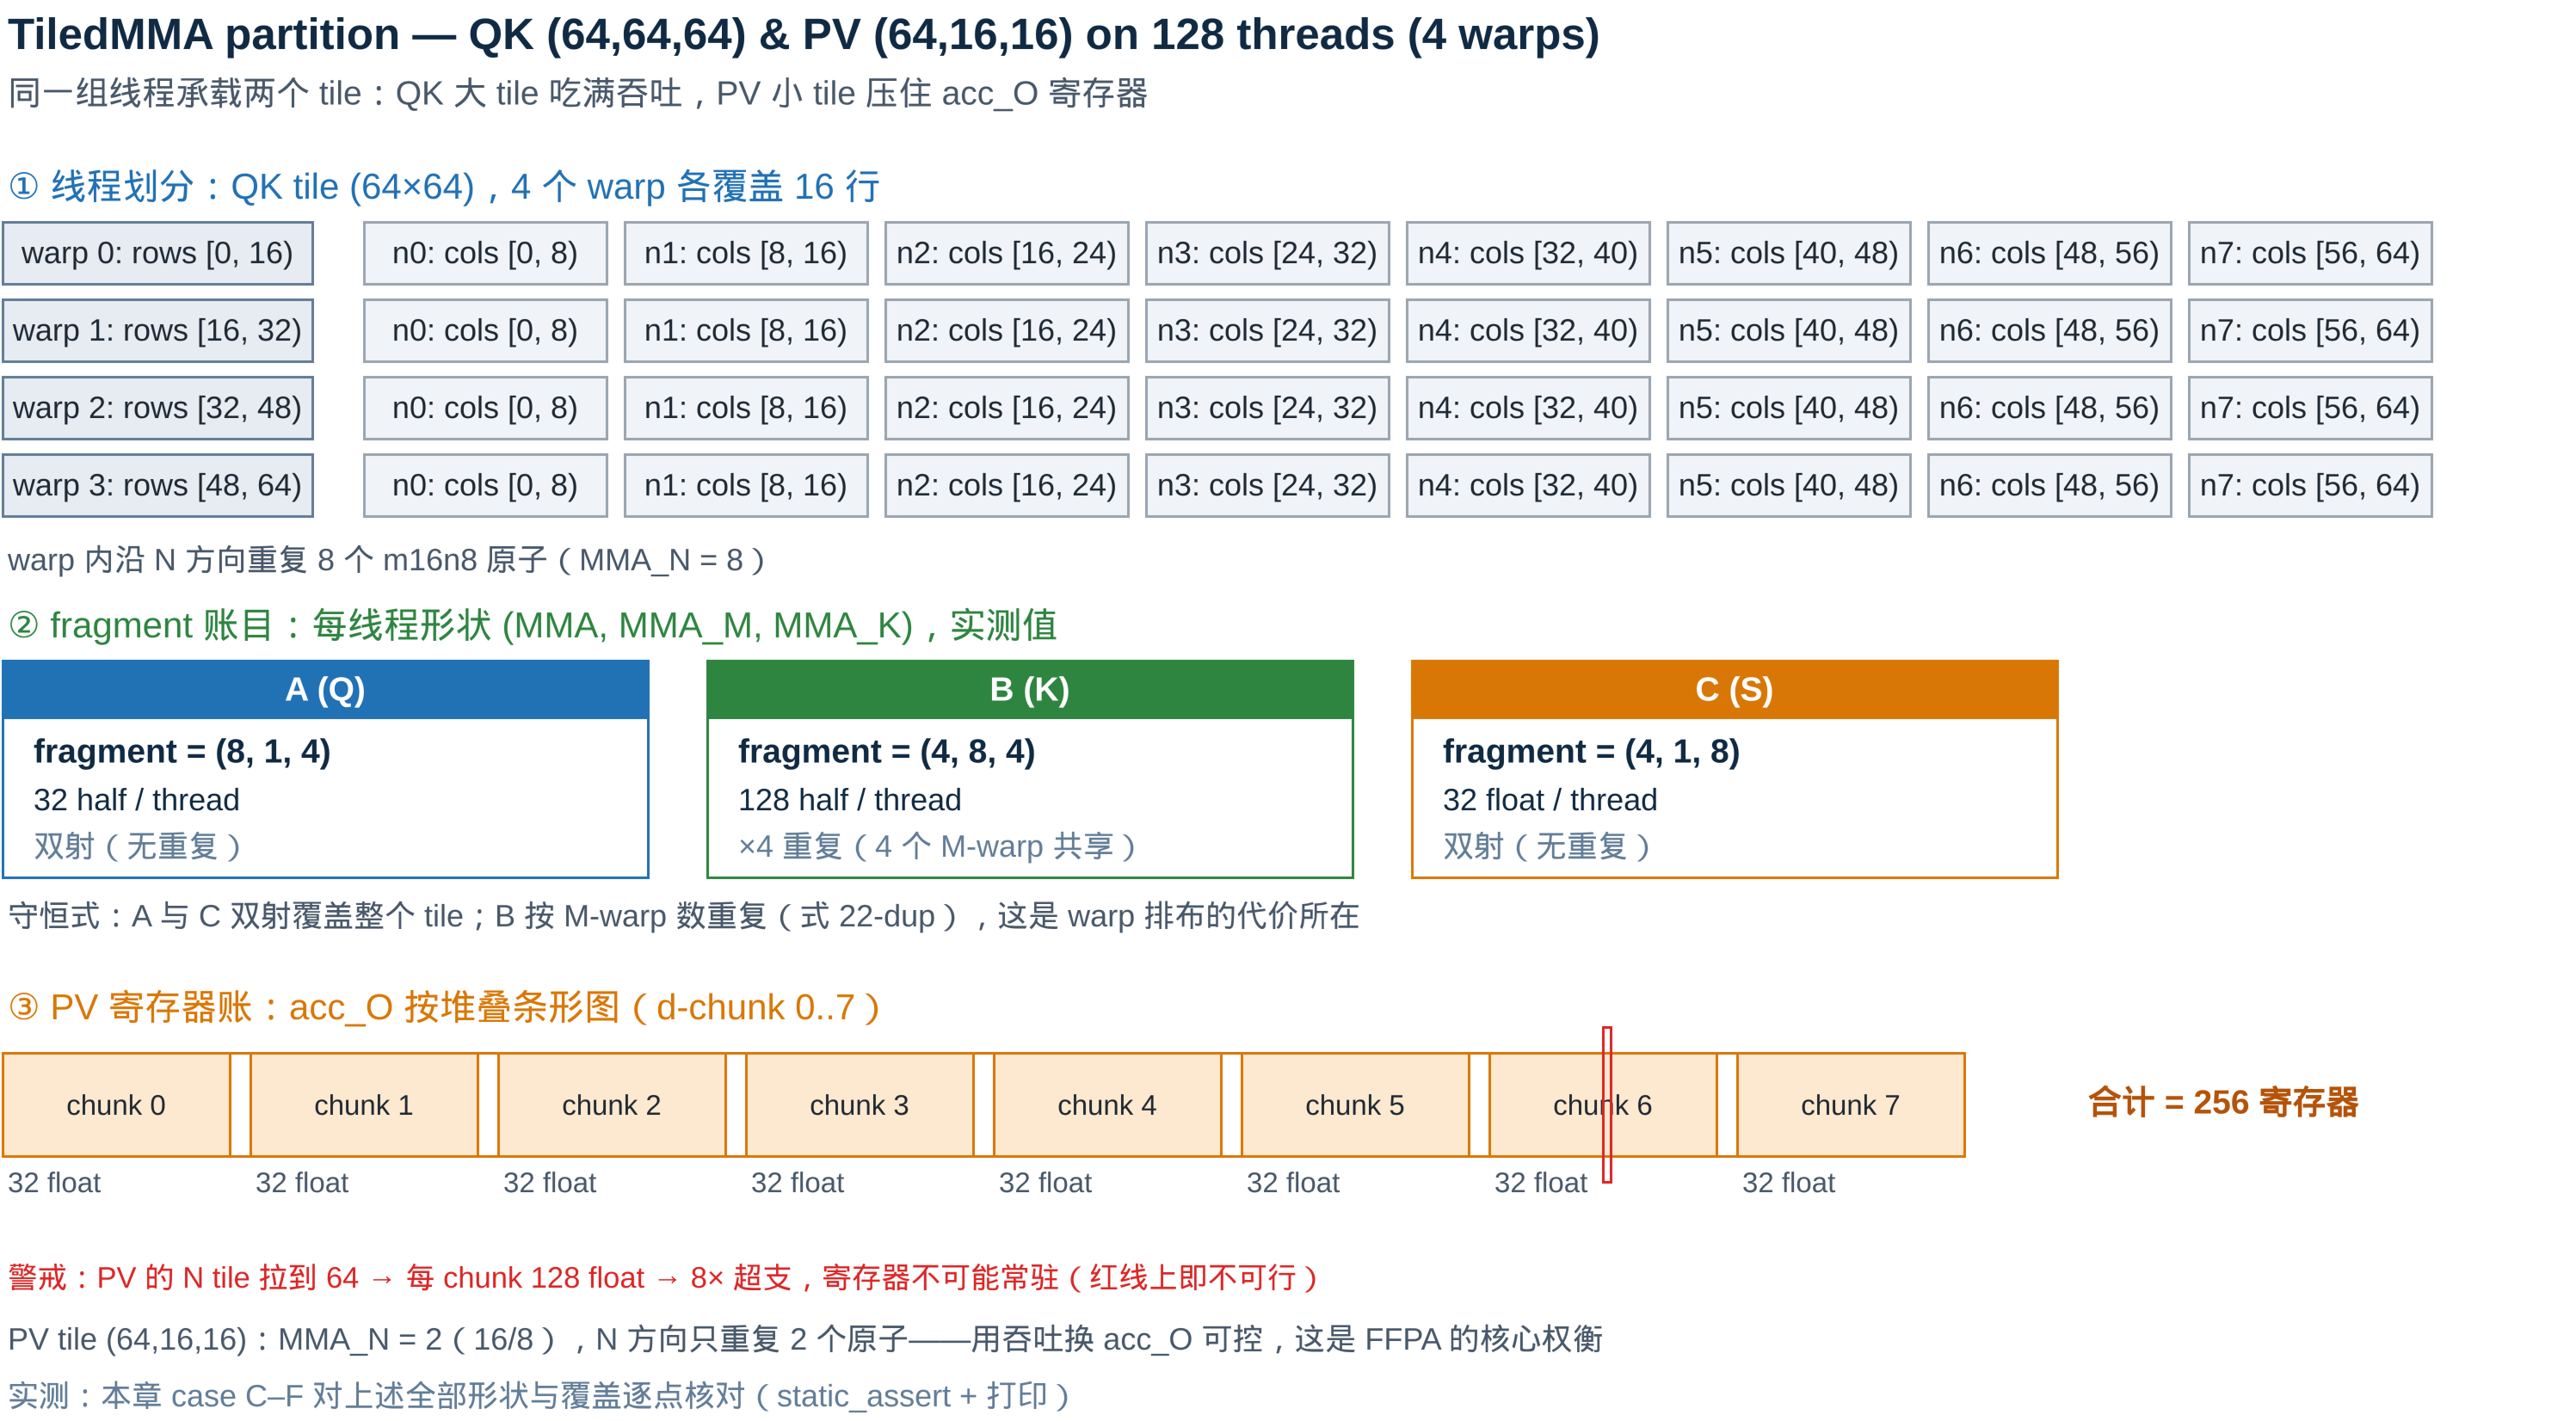
\includegraphics[width=0.92\textwidth]{figures/drawio/fig-22-1-tiledmma/fig-22-1.png}
\begin{tikzpicture}[font=\tiny, x=0.016cm, y=-0.016cm]
  \node[anchor=west, font=\footnotesize\bfseries] at (40,29)
    {TiledMMA partition —— QK $(M,N,K)=(64,64,64)$ \& PV $(M,N,K)=(64,16,16)$ on 128 threads (4 warps)};
  \node[anchor=west, font=\scriptsize] at (40,52)
    {同组线程承载两个 tile：QK 大 tile 达吞吐上限，PV 小 tile 控制 per-call 视图与临时开销};
  \node[anchor=west, font=\scriptsize, text=tkBlue] at (40,88)
    {\textcircled{1} 线程划分：QK tile $(64\times64)$，4 个 warp 各覆盖 16 行};
  \foreach \rr/\wr in {0/{warp 0: rows [0, 16)}, 1/{warp 1: rows [16, 32)},
                       2/{warp 2: rows [32, 48)}, 3/{warp 3: rows [48, 64)}}{
    \ifcase\rr
      \def\wfill{colorx4!16} \def\wline{colorx4!65}%
    \or
      \def\wfill{colorx5!16} \def\wline{colorx5!65}%
    \or
      \def\wfill{colorx6!16} \def\wline{colorx6!65}%
    \else
      \def\wfill{colorx7!16} \def\wline{colorx7!65}%
    \fi
    \node[draw=\wline, fill=\wfill, minimum width=1.92cm, minimum height=0.384cm,
          inner sep=0pt] at (100,{114+30*\rr})
      {{\fontsize{4.6}{5.4}\selectfont\wr}};
    \foreach \cc in {0,...,7}{
      \node[draw=gray!45, fill=gray!5, minimum width=1.504cm, minimum height=0.384cm,
            inner sep=0pt] at ({227+101*\cc},{114+30*\rr})
        {{\fontsize{4.6}{5.4}\selectfont n\cc: cols [\the\numexpr8*\cc\relax,
          \the\numexpr8*\cc+8\relax)}};
    }
  }
  \node[anchor=west, font=\tiny] at (40,233)
    {warp 内沿 N 方向重复 8 个 m16n8 原子（MMA\_N $= 8$）};
  \node[anchor=west, font=\scriptsize, text=tkGreen] at (40,258)
    {\textcircled{2} fragment 明细：每线程形状 $(\mathrm{MMA}, \mathrm{MMA\_M}, \mathrm{MMA\_K})$，实测值};
  \foreach \cx/\hd/\col in {165/{A (Q)}/tkBlue, 438/{B (K)}/tkGreen, 711/{C (S)}/tkOrange}{
    \node[draw=\col, fill=white, minimum width=4.0cm, minimum height=1.344cm,
          inner sep=0pt] at (\cx,314) {};
    \node[fill=\col, text=white, font=\scriptsize\bfseries, minimum width=4.0cm,
          minimum height=0.352cm, inner sep=0pt] at (\cx,283) {\hd};
  }
  \node[anchor=west, font=\scriptsize\bfseries] at (50,307) {fragment $= (8, 1, 4)$};
  \node[anchor=west, font=\tiny] at (50,326) {32 half / thread};
  \node[anchor=west, font=\tiny, text=gray!90] at (50,344) {双射（无重复）};
  \node[anchor=west, font=\scriptsize\bfseries] at (323,307) {fragment $= (4, 8, 4)$};
  \node[anchor=west, font=\tiny] at (323,326) {128 half / thread};
  \node[anchor=west, font=\tiny, text=gray!90] at (323,344) {$\times4$ 重复（4 个 M-warp 共享）};
  \node[anchor=west, font=\scriptsize\bfseries] at (596,307) {fragment $= (4, 1, 8)$};
  \node[anchor=west, font=\tiny] at (596,326) {32 float / thread};
  \node[anchor=west, font=\tiny, text=gray!90] at (596,344) {双射（无重复）};
  \node[anchor=west, font=\tiny] at (40,371)
    {守恒式：A 与 C 双射覆盖整个 tile；B 按 M-warp 数重复（式~\eqref{eq:22-dup}），
     这是 warp 排布的代价所在};
  \node[anchor=west, font=\scriptsize, text=tkOrange] at (40,406)
    {\textcircled{3} PV 寄存器占用：acc\_O 按堆叠条形图（d-chunk 0--7）};
  \foreach \k in {0,...,7}{
    \node[draw=tkOrange!70, fill=tkFillOrange, minimum width=1.408cm, minimum height=0.64cm,
          inner sep=0pt] at ({84+96*\k},444) {chunk \k};
    \node[font=\tiny, text=gray!90] at ({84+96*\k},491) {32 float};
  }
  \node[anchor=west, font=\scriptsize\bfseries, text=tkOrange!80!black] at (846,443)
    {合计 $=256$ 个 f32 逻辑值};
  \draw[tkRed, very thick] (708,414) -- (708,474);
  \node[anchor=west, font=\tiny, text=tkRed] at (40,511)
    {注意：232 的 WS 配额会更早触及；总量 256 也已超过 255 硬上限，必须 spill，
     Split-D 本身并不降低 acc\_O 总量};
  \node[anchor=west, font=\tiny] at (40,535)
    {PV tile $(64,16,16)$：MMA\_N $= 2$（$16/8$），N 方向只重复 2 个原子，
     控制 per-call C 视图与 B fragment 的临时开销};
  \node[anchor=west, font=\tiny, text=gray!90] at (40,559)
    {实测：本章 case~C--F 对上述全部形状与覆盖逐点核对（\texttt{static\_assert} $+$ 打印）};
\end{tikzpicture}
\caption{TiledMMA partition：QK 的 $64\times64$ tile 上，4 个 warp 各覆盖
16 行，warp 内 N 方向重复 8 个原子；A/B/C 三种 fragment 的每线程形状与
重复因子（式~\eqref{eq:22-dup}）。下半部分是 PV 的 $(64,16,16)$ tile：
N 方向只重复 2 个原子，代价换来 per-call C 视图与拷贝粒度可控（8 个
d-chunk 各自拷回，acc\_O 总量只由 $D$ 决定——$8\times32=256$ 个 f32
逻辑值，与 N tile 无关；这些逻辑值超过 255 个寄存器的硬上限时需要 spill，
N tile 取 64 只是单次调用的 C fragment 临时 4 倍）。}
\label{fig:22-1}
\end{figure}

\begin{figure}[htbp]
\centering
% was: 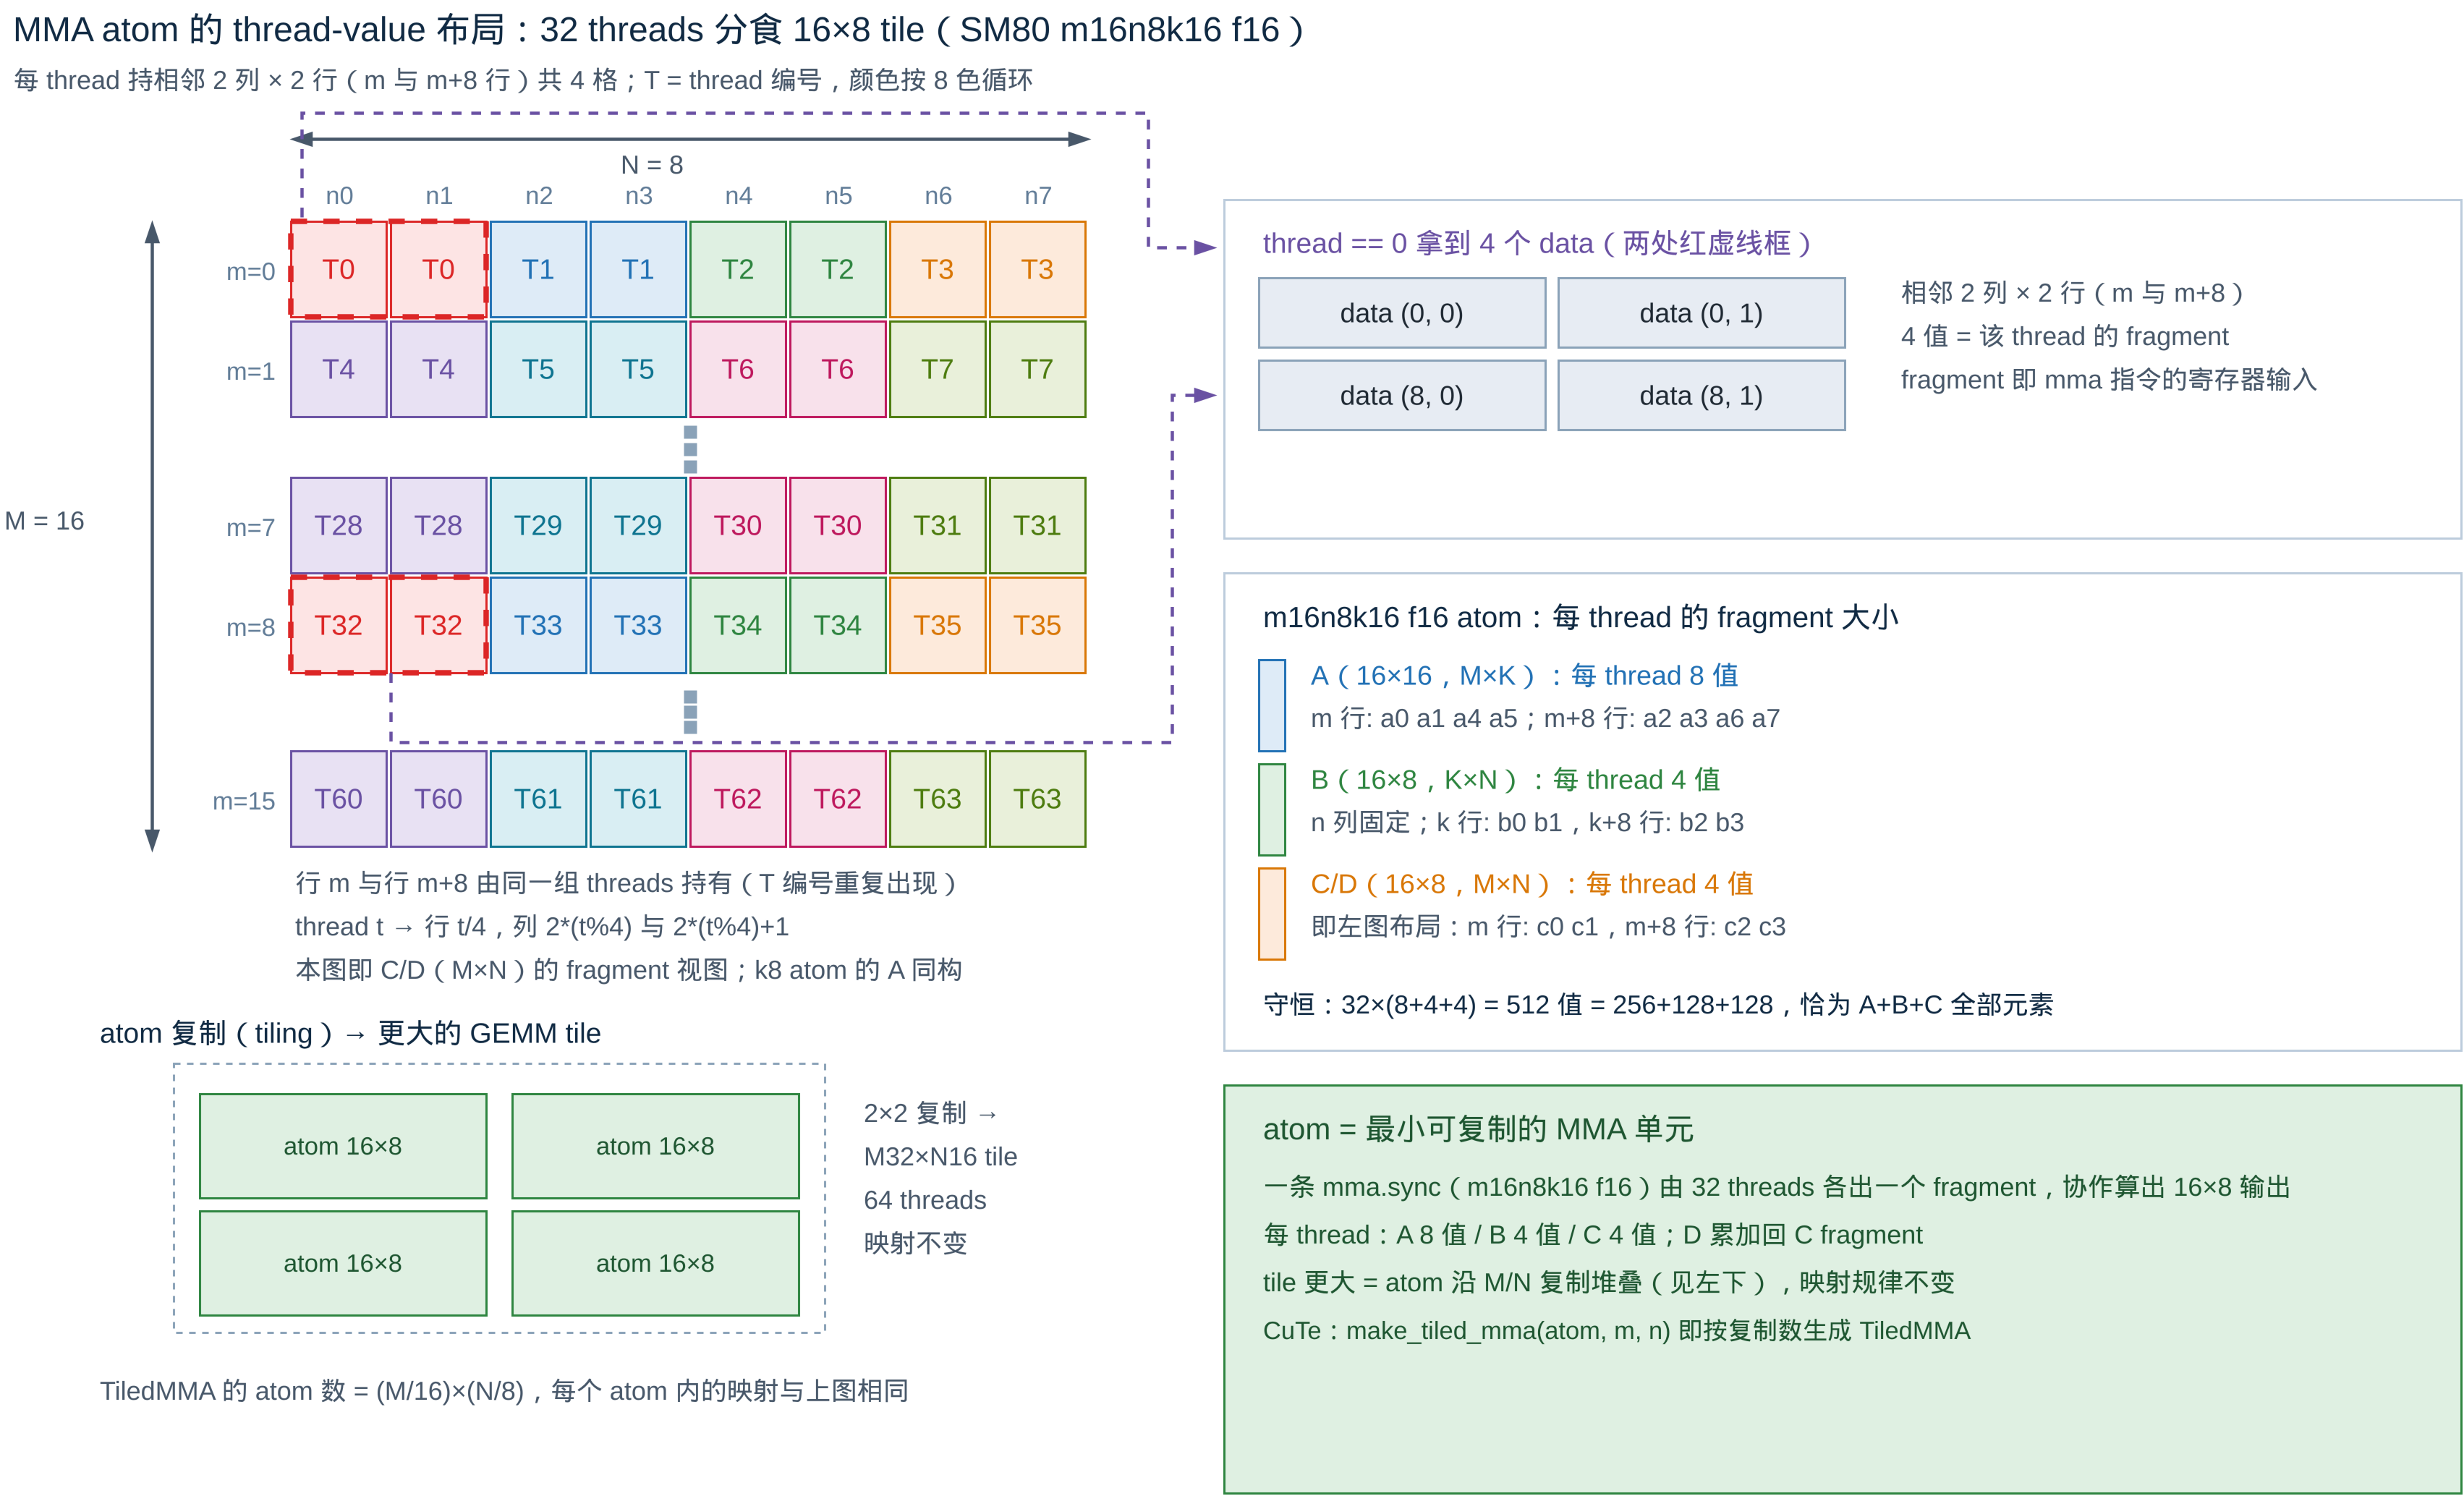
\includegraphics[width=0.95\textwidth]{figures/drawio/fig-22-2-mma-atom-fragments/fig-22-2.png}
\begin{tikzpicture}[font=\tiny, x=0.015cm, y=-0.015cm]
  \node[anchor=west, font=\scriptsize\bfseries] at (20,21)
    {MMA atom 的 thread-value 布局：32 threads 平分 $16\times8$ tile（SM80 m16n8k16 f16）};
  \node[anchor=west, font=\tiny] at (20,45)
    {每 thread 持相邻 2 列 $\times$ 2 行（$m$ 与 $m{+}8$ 行）共 4 格；T $=$ thread
     编号，颜色按 8 色循环};
  \draw[{Stealth[length=1.6mm]}-{Stealth[length=1.6mm]}, gray!80, thin] (150,72) -- (518,72);
  \node[font=\tiny] at (345,83) {N $= 8$};
  \draw[{Stealth[length=1.6mm]}-{Stealth[length=1.6mm]}, gray!80, thin] (86,110) -- (86,400);
  \node[anchor=east, font=\tiny] at (78,250) {M $= 16$};
  \foreach \cc in {0,...,7}{
    \node[font=\tiny, text=gray!80] at ({172+46*\cc},98) {n\cc};
  }
  \foreach \mm/\cy in {0/132, 1/178, 7/250, 8/296, 15/376}{
    \node[anchor=east, font=\tiny, text=gray!80] at (144,\cy) {m$=$\mm};
    \foreach \cc in {0,...,7}{
      \pgfmathtruncatemacro{\grp}{mod(\mm*4 + int(\cc/2), 8)}
      \pgfmathtruncatemacro{\tn}{\mm*4 + int(\cc/2)}
      \ifcase\grp
        \node[draw=colorx1!65!black, fill=colorx1!42, text=colorx1!85!black,
              minimum width=0.66cm, minimum height=0.66cm, inner sep=0pt]
          at ({172+46*\cc},\cy) {T\tn};
      \or
        \node[draw=colorx2!65!black, fill=colorx2!42, text=colorx2!85!black,
              minimum width=0.66cm, minimum height=0.66cm, inner sep=0pt]
          at ({172+46*\cc},\cy) {T\tn};
      \or
        \node[draw=colorx3!65!black, fill=colorx3!42, text=colorx3!85!black,
              minimum width=0.66cm, minimum height=0.66cm, inner sep=0pt]
          at ({172+46*\cc},\cy) {T\tn};
      \or
        \node[draw=colorx4!65!black, fill=colorx4!42, text=colorx4!85!black,
              minimum width=0.66cm, minimum height=0.66cm, inner sep=0pt]
          at ({172+46*\cc},\cy) {T\tn};
      \or
        \node[draw=colorx5!65!black, fill=colorx5!42, text=colorx5!85!black,
              minimum width=0.66cm, minimum height=0.66cm, inner sep=0pt]
          at ({172+46*\cc},\cy) {T\tn};
      \or
        \node[draw=colorx6!65!black, fill=colorx6!42, text=colorx6!85!black,
              minimum width=0.66cm, minimum height=0.66cm, inner sep=0pt]
          at ({172+46*\cc},\cy) {T\tn};
      \or
        \node[draw=colorx7!65!black, fill=colorx7!42, text=colorx7!85!black,
              minimum width=0.66cm, minimum height=0.66cm, inner sep=0pt]
          at ({172+46*\cc},\cy) {T\tn};
      \else
        \node[draw=colorx8!65!black, fill=colorx8!42, text=colorx8!85!black,
              minimum width=0.66cm, minimum height=0.66cm, inner sep=0pt]
          at ({172+46*\cc},\cy) {T\tn};
      \fi
    }
  }
  \foreach \yy in {206,214,222,330,338,346}{
    \fill[gray!70] (334,\yy) circle (0.05cm);
  }
  \draw[tkRed, dashed, thick] (150,110) rectangle (240,154);
  \draw[tkRed, dashed, thick] (150,274) rectangle (240,318);
  \node[anchor=west, font=\tiny] at (150,415)
    {行 $m$ 与行 $m{+}8$ 由同一组 threads 持有（T 编号重复出现）};
  \node[anchor=west, font=\tiny] at (150,435)
    {thread $t \to$ 行 $t/4$，列 $2(t \bmod 4)$ 与 $2(t \bmod 4){+}1$};
  \node[anchor=west, font=\tiny] at (150,455)
    {本图即 C/D（M$\times$N）的 fragment 视图；k8 atom 的 A 同构};
  \draw[gray!45, thin] (580,100) rectangle (1150,256);
  \node[anchor=west, font=\scriptsize, text=tkPurple] at (596,120)
    {thread $==$ 0 拿到 4 个 data（两处红虚线框）};
  \foreach \cx/\cy/\tx in {662/152/{data (0, 0)}, 800/152/{data (0, 1)},
                           662/190/{data (8, 0)}, 800/190/{data (8, 1)}}{
    \node[draw=gray!50, fill=gray!12, minimum width=1.98cm, minimum height=0.48cm,
          inner sep=0pt] at (\cx,\cy) {\tx};
  }
  \node[anchor=west, font=\tiny, text=gray!90] at (890,143) {相邻 2 列 $\times$ 2 行（$m$ 与 $m{+}8$）};
  \node[anchor=west, font=\tiny, text=gray!90] at (890,165) {4 值 $=$ 该 thread 的 fragment};
  \node[anchor=west, font=\tiny, text=gray!90] at (890,187) {fragment 即 mma 指令的寄存器输入};
  \draw[gray!45, thin] (580,272) rectangle (1150,492);
  \node[anchor=west, font=\scriptsize] at (596,292)
    {m16n8k16 f16 atom：每 thread 的 fragment 大小};
  \node[fill=tkFillBlue, draw=tkBlue!60, minimum width=0.18cm, minimum height=0.63cm,
        inner sep=0pt] at (602,333) {};
  \node[anchor=west, font=\tiny, text=tkBlue] at (618,319)
    {A（$16\times16$，M$\times$K）：每 thread 8 值};
  \node[anchor=west, font=\tiny] at (618,341)
    {m 行: a0 a1 a4 a5；m$+$8 行: a2 a3 a6 a7};
  \node[fill=tkFillGreen, draw=tkGreen!60, minimum width=0.18cm, minimum height=0.63cm,
        inner sep=0pt] at (602,381) {};
  \node[anchor=west, font=\tiny, text=tkGreen] at (618,367)
    {B（$16\times8$，K$\times$N）：每 thread 4 值};
  \node[anchor=west, font=\tiny] at (618,389)
    {n 列固定；k 行: b0 b1，k$+$8 行: b2 b3};
  \node[fill=tkFillOrange, draw=tkOrange!70, minimum width=0.18cm, minimum height=0.63cm,
        inner sep=0pt] at (602,429) {};
  \node[anchor=west, font=\tiny, text=tkOrange!80!black] at (618,415)
    {C/D（$16\times8$，M$\times$N）：每 thread 4 值};
  \node[anchor=west, font=\tiny] at (618,437)
    {即左图布局：m 行: c0 c1，m$+$8 行: c2 c3};
  \node[anchor=west, font=\tiny] at (596,471)
    {守恒：$32\times(8+4+4) = 512$ 值 $= 256+128+128$，恰为 $A+B+C$ 全部元素};
  \node[draw=tkGreen, fill=tkFillGreen, minimum width=8.55cm, minimum height=2.82cm,
        inner sep=0pt] at (865,602) {};
  \node[anchor=west, font=\scriptsize, text=tkGreen!70!black] at (596,528)
    {atom $=$ 最小可复制的 MMA 单元};
  \node[anchor=west, font=\tiny, text=tkGreen!70!black] at (596,555)
    {一条 \texttt{mma.sync}（m16n8k16 f16）由 32 threads 各出一个 fragment，};
  \node[anchor=west, font=\tiny, text=tkGreen!70!black] at (596,577)
    {协作算出 $16\times8$ 输出};
  \node[anchor=west, font=\tiny, text=tkGreen!70!black] at (596,599)
    {每 thread：A 8 值 / B 4 值 / C 4 值；D 累加回 C fragment};
  \node[anchor=west, font=\tiny, text=tkGreen!70!black] at (596,621)
    {tile 更大 $=$ atom 沿 M/N 复制堆叠（见左下），映射规律不变};
  \node[anchor=west, font=\tiny, text=tkGreen!70!black] at (596,643)
    {CuTe：\texttt{make\_tiled\_mma(atom, m, n)} 即按复制数生成 TiledMMA};
  \node[anchor=west, font=\scriptsize] at (60,484) {atom 复制（tiling）$\to$ 更大的 GEMM tile};
  \draw[gray!60, dashed, thin] (96,498) rectangle (396,622);
  \foreach \cx/\cy in {174/536, 318/536, 174/590, 318/590}{
    \node[draw=tkGreen, fill=tkFillGreen, text=tkGreen!70!black, minimum width=1.98cm,
          minimum height=0.72cm, inner sep=0pt] at (\cx,\cy) {atom $16\times8$};
  }
  \node[anchor=west, font=\tiny] at (412,521) {2$\times$2 复制 $\to$};
  \node[anchor=west, font=\tiny] at (412,541) {M32$\times$N16 tile};
  \node[anchor=west, font=\tiny] at (412,561) {64 threads};
  \node[anchor=west, font=\tiny] at (412,581) {映射不变};
  \node[anchor=west, font=\tiny] at (60,649)
    {TiledMMA 的 atom 数 $= (\mathrm{M}/16)\times(\mathrm{N}/8)$，每个 atom 内的映射与上图相同};
  \draw[-{Stealth[length=2mm]}, tkPurple, dashed, thick]
    (152,108) -- (152,64) -- (545,64) -- (545,122) -- (576,122);
  \draw[-{Stealth[length=2mm]}, tkPurple, dashed, thick]
    (196,320) -- (196,350) -- (556,350) -- (556,190) -- (576,190);
\end{tikzpicture}
\caption{m16n8k16 atom 的 C fragment thread-value 映射：thread $t$ 持行 $t/4$ 与 $t/4+8$、列 $2(t\bmod 4)$ 与 $2(t\bmod 4)+1$ 共 4 值——行 $m$ 与 $m+8$ 由同组线程重复持有。三个操作数每线程 A 8 值 / B 4 值 / C 4 值，守恒式 $32\times(8+4+4)=512$。更大的 tile 只是 atom 沿 M/N 的复制堆叠，thread-value 规律不变——\texttt{make\_\allowbreak{}tiled\_\allowbreak{}mma} 的构造基础。重建自 @竹熙佳处《写给大家看的 CuTe 教程：tiled mma》。}
\label{fig:22-2}
\end{figure}

\section{性能分析}

本章同样没有独立 bench：TiledMMA 的开销体现在它选择的 tile 形状上，端到端
数字在第~\ref{ch:19}、\ref{ch:26}~章（FFPA）与第~\ref{ch:24}~章（HGEMM）。
本节把 tile 选择转化为三个可计算的指标。

\textbf{指标一（寄存器）}：acc\_O $=kD_{\mathrm{chunks}}\times\mathrm{ThrLD}
\times\mathrm{MMA}_M\times\mathrm{MMA}_N\times\mathrm{Nrep}$（ThrLD 是单个
atom 每线程的 C 值数 $4$，Nrep 是 chunk 内 N 方向的重复数 $64/16=4$）
$=8\times4\times1\times2\times4=256$。PV 的
$\mathrm{MMA}_N = 2$（$16/8$）时每个 $64\times64$ d-chunk 每线程是 32 个
f32 逻辑累加值；$D=512$ 时 $8$ 个 chunk 共 256 个，已超过 255 个寄存器的
硬上限，需要 spill。tile N=64 时单次 gemm 调用的 C fragment 从 8 值涨到
32 值（4 倍），acc\_O 的逻辑总量（8 chunk $\times$ 32 $=$ 256 float）不变，
N tile 带来的增量超支在每次调用的临时视图与 B fragment，不在累加器。
FFPA 注释里 PV 保持小 tile 的算术依据正在于此：压的是每次调用的
临时开销，而非 acc\_O 的总量。

\textbf{指标二（重复因子）}：B 的 fragment 按 M-warp 数重复（式~\eqref{eq:22-dup}）。
QK 用 $(4,1,1)$ 排布时 B 重复 4 倍（$4\times32=128$ 个 half/线程），
A 不重复，A+B 共 160 half/线程；若改成 $(2,2,1)$（各方向 2 个 warp），A 与 B
各重复 2 倍，A+B 变为 $64+64=128$ half/线程（降约 20\%），warp 覆盖的行也从
16 行变成 32 行。warp 排布同时改变“谁重复”和重复总量，需要按两者共同权衡。

\textbf{指标三（指令数）}：一次 TiledMMA 调用的指令数
$=\mathrm{MMA}_M\times\mathrm{MMA}_N\times\mathrm{MMA}_K$，注意这是
\emph{每线程（每 warp）}的条数。QK 的 $(1,8,4)=32$ 条是每个 warp 的量，
覆盖该 warp 的 $16\times64\times64$；4 个 warp 共 128 条才铺满 CTA 的
$64\times64\times64$：512 KFLOP/128 条，每条 $16\times8\times16$ 共
$4096$ FLOP（约 4.1 KFLOP）；PV 同口径：$(1,2,4)=8$ 条/warp 覆盖
$16\times16\times64$，CTA 的 $64\times16\times64$ 需 4 warp 共 32 条。
两个 tile 都让每条 MMA 指令用满原子尺寸，没有浪费，因为它们都是从
$\mathrm{AtomShape}$ 出发、只用排布与 tile 尺寸做整数分块推出来的。

口径说明：本节所有数字都是 host 端类型推导的实测值（
\texttt{partition\_\allowbreak{}fragment\_\allowbreak{}*} 的形状），不含计时数据；FFPA 的
TFLOPS 对照见第~\ref{ch:19}~章的表与第~\ref{ch:26}~章的 kernel 分析。
还有一条引用规则：ffpa\_attn.cuh L16--18 的头注释给出\textbf{SM120a
RTX PRO 5000：cuDNN SDPA 57.2 TFLOPS、FFPA TMA WS 110.7 TFLOPS（1.94x）}，
除法自洽（$110.7/57.2=1.94$），但设备口径是 \emph{RTX PRO 5000}（本机），
与 README 的 5090 口径不同。\textbf{引用这类比值时必须带上设备名}，
同一份代码在两块卡上的比值并不相等。

\section{常见坑}

\textbf{坑一：fragment 必须先清零/初始化。}
\texttt{partition\_\allowbreak{}fragment\_\allowbreak{}C} 返回的是一块未定义寄存器数组的视图，
\emph{不会}置零。FFPA 里 \texttt{tCrS} 定义后立即 \texttt{clear(tCrS)}，
acc\_O 用显式循环清零（L173--176）。漏掉这一步的后果不是崩溃，而是把
未初始化寄存器当累加初值，编译器还可能把整个累加链折叠成垃圾值，
表现为结果偶尔对、偶尔全错。同理，被 \texttt{convert\_\allowbreak{}layout\_\allowbreak{}acc\_\allowbreak{}Aregs}
重解释的 $P$ 必须确保所有 32 个槽位都已被 softmax 写过。

\textbf{坑二：两个 TiledMMA 的 fragment 不能互换。}
QK 的 C fragment 是 $(4,1,8)$，PV 的 A fragment 是 $(8,1,4)$：形状、元素
类型（float/half）都不同。FFPA 的复用之所以成立，是因为它做了
\emph{类型转换 $+$ 布局重解释}两步（\texttt{convert\_\allowbreak{}type} $+$
\texttt{convert\_\allowbreak{}layout\_\allowbreak{}acc\_\allowbreak{}Aregs}），且只对 m16n8k16 这一族成立。
把 C 直接交给 PV 是典型的静默错位。

\textbf{坑三：tile 必须是原子的整数倍，warp 排布必须与线程数自洽。}
$\mathrm{perm\_M}$ 不是 $16$ 的倍数、或 $\mathrm{ThrM}\times 32$ 与
\texttt{blockDim} 不一致时，partition 会产生多余/缺失的 remainder mode
（编译期静态断言或运行期越界）。判据：\texttt{size(mma)} 是线程数的权威来源，
用它来配 \texttt{dim3 block\allowbreak{}(size\allowbreak{}(mma))}。

\textbf{坑四：\texttt{get\_slice} 的坐标是 $(\mathrm{ThrV},(\mathrm{ThrM},
\mathrm{ThrN/K}))$ 三层，不是 warp 内 lane $+$ 全局 warp 两层。}
FFPA 的 $128$ 线程排布是 $(\mathrm{ThrV}=32,\mathrm{ThrM}=4)$，因此
线程 $t$ 的行带是 $16\lfloor t/32\rfloor$；把 $\mathrm{ThrM}$ 当成
线程号对 4 取模会得到完全错误的 warp 映射（本章测试 case~E 专门核对
这条）。

\textbf{坑五：\texttt{partition\_\allowbreak{}fragment\_\allowbreak{}A} 的输入决定 fragment 的
MMAK 大小，但不改变 atom 约定。}
QK 的 A 在 $(64,64)$ 上是 $(8,1,4)$，在 $(64,16)$ 上就是 $(8,1,1)$；
$\mathrm{MMA}_K$ 随输入 K 长度变化。写循环时要用
\texttt{size\allowbreak{}<2>\allowbreak{}(fragment)} 作为 K 循环上界（第~\ref{ch:21}~章 kernel 的
\texttt{num\_k\_steps} 就是这么来的），不要写死。

\textbf{坑六：C fragment 的行列不是直觉顺序。}
$(4,1,8)$ 的 4 个 float 对应 2 行 $\times$ 2 列，同一个 lane 的第 0、1 个
元素在同一行相邻两列，第 2、3 个在 $+8$ 行处。想按 (row, col) 遍历必须先做
\texttt{convert\_\allowbreak{}layout\_\allowbreak{}acc\_\allowbreak{}rowcol}（L2315--2333 推导）；直接用
\texttt{fragment\allowbreak{}(idx)} 当矩阵元素是最常见的读错方式。

\section{面试要点速查}

\textbf{Q1：MMA\_Atom 与 TiledMMA 的区别？}\\
A：MMA\_Atom 是一条指令的抽象（Shape\_MNK $+$ 三份 TV layout $+$ ThrID）；
TiledMMA 是把原子铺满一个 tile 的类型，多出 warp 排布与 tile 尺寸两个
参数，并提供 \texttt{partition\_\allowbreak{}fragment\_\allowbreak{}*}。

\textbf{Q2：\texttt{make\_\allowbreak{}tiled\_\allowbreak{}mma} 的第二个、第三个参数分别是什么？}\\
A：第二个是 warp 排布（\texttt{Atom\allowbreak{}Layout\allowbreak{}MNK}，决定 \texttt{Thr\allowbreak{}M/\allowbreak{}Thr\allowbreak{}N/\allowbreak{}Thr\allowbreak{}K}
与重复因子），第三个是目标 tile 尺寸（\texttt{Permutation\allowbreak{}MNK}，含 K）。
FFPA：排布 $(4,1,1)$，tile $(64,64,16)$ 与 $(64,16,16)$。

\textbf{Q3：fragment 的三个 mode 是什么？}\\
A：$(\mathrm{MMA}, \mathrm{MMA}_M, \mathrm{MMA}_K)$：每个原子的值数、
M 方向原子重复、K 方向原子重复（C 的第三 mode 是
$\mathrm{MMA}_N$）。它们是式~\eqref{eq:22-thrfrg-4} 第 (4) 步之后的余量。

\textbf{Q4：为什么 A 的 fragment 有时会重复？}\\
A：warp 排布如果在 N 方向有分片，不同 N-warp 需要同一份 A，于是 A 被
重复持有（重复因子 $=$ N-warp 数）；B 同理（因子 $=$ M-warp 数）。
式~\eqref{eq:22-dup}。

\textbf{Q5：\texttt{get\_\allowbreak{}slice\allowbreak{}(t)} 内部发生了什么？}\\
A：把整数 $t$ 按 \texttt{Thr\allowbreak{}Layout\allowbreak{}VMNK} 分解成
$(\mathrm{ThrV},(\mathrm{ThrM},\mathrm{ThrN}),\mathrm{ThrK})$，得到一个
只属于该线程的 ThrMMA，后续 partition 都基于它。

\textbf{Q6：QK 与 PV 为什么要用两个 TiledMMA？}\\
A：目标不同。QK 要一次覆盖整个 $S$（N $=64$）省循环；PV 的 N 控制单次
调用的 C 视图、B fragment 与拷贝粒度，而 acc\_O 的逻辑总量由输出形状和
线程数决定，不随 N tile 缩小。两者共享同一套 128 线程排布，fragment 通过
类型转换 $+$ 布局重解释衔接。

\textbf{Q7：\texttt{tile\_\allowbreak{}size\allowbreak{}<I>\allowbreak{}(mma)} 有什么用？}\\
A：它是 TiledMMA 对外的尺寸接口，也是 \texttt{make\_\allowbreak{}tiled\_\allowbreak{}copy\_\allowbreak{}A/\allowbreak{}B/\allowbreak{}C}
推导 S$\to$R 拷贝 tiler 的来源（第~\ref{ch:21}~章式~(21-mtca)）。
TiledMMA 与 TiledCopy 通过它解耦：改 tile 不影响拷贝代码。

\textbf{Q8：tile 的 N 尺寸调节什么？}\\
A：单次调用 C fragment 每线程元素数 $=\mathrm{MMA}\times\mathrm{MMA}_M\times
\mathrm{MMA}_N$，而 $\mathrm{MMA}_N = \mathrm{tile}_N/(\mathrm{atom}_N\,\mathrm{ThrN})$
（本章 FFPA 的 $\mathrm{ThrN}=1$，故可简写为 $\mathrm{tile}_N/\mathrm{atom}_N$）：
tile N 增大时 per-call C 视图与 B fragment 随之线性增长，S$\to$R 拷贝
粒度变粗；acc\_O 的逻辑总量（$D=512$ 时为 256 个 f32 值）不变，超过
255 个寄存器时需要 spill。PV 因此取 $\mathrm{tile}_N=16$
（$64\times16\times16$）来控制单次调用的临时开销。

\section{最小测试与动手实验}

测试文件：\texttt{book/\allowbreak{}tests/\allowbreak{}ch22\_\allowbreak{}tiled\_\allowbreak{}mma.cu}（host-only：只做类型与
partition 断言，不启动 kernel；直接 include
\texttt{.\allowbreak{}.\allowbreak{}/\allowbreak{}.\allowbreak{}.\allowbreak{}/\allowbreak{}ffpa\_\allowbreak{}attn.\allowbreak{}cuh} 以核对真实的 traits）。六个 case：

\begin{itemize}
  \item \textbf{A 原子 fragment 公式}：对
        \texttt{SM80\_\allowbreak{}16x8x16\_\allowbreak{}F32\allowbreak{}F16\allowbreak{}F16\allowbreak{}F32\_\allowbreak{}TN} 的 A/B/C 三个 layout，
        逐 lane、逐值核对手推公式式~\eqref{eq:22-atom-a}--\eqref{eq:22-atom-c}
        （$32\times8$、$32\times4$、$32\times4$ 个逐值断言，另加 7 条形状/值数断言，
        合计 519 checks）；
  \item \textbf{B tile\_size 与线程数}：QK/PV 的 \texttt{tile\_size} 为
        $(64,64,16)/(64,16,16)$、\texttt{size(mma)}$=128$；对象
        \texttt{FFPAAttn\allowbreak{}Split\allowbreak{}DCu\allowbreak{}Te\allowbreak{}Traits\allowbreak{}<512>}
        并与手写的
        \texttt{make\_\allowbreak{}tiled\_\allowbreak{}mma} 构造做类型一致性检查；
  \item \textbf{C fragment 形状}：QK 在 $(64,64)$ 上 A/B/C 每线程
        $(8,1,4)/(4,8,4)/(4,1,8)$，PV 为 $(8,1,4)/(4,2,1)/(4,1,8)$；
        逐项核对元素数；
  \item \textbf{D 守恒与重复因子}：C 的覆盖是双射（$128\times32=4096=
        64\times64$）且 A 也是；B 恰好 4 倍重复（每元素被 4 个
        (线程, 值) 对覆盖）；
  \item \textbf{E warp 边界}：QK 的 C fragment 逐线程回投坐标，四个 warp 的
        行带为 $[0,16),[16,32),[32,48),[48,64)$，互不重叠；
  \item \textbf{F PV 的 acc\_O 占用}：
        \texttt{partition\_\allowbreak{}fragment\_\allowbreak{}C\allowbreak{}(tiled\_\allowbreak{}mma\_\allowbreak{}pv,\allowbreak{} Shape\allowbreak{}<\_\allowbreak{},\allowbreak{}64,\allowbreak{}\_\allowbreak{}64>\{\})}
        每线程 32 个值，$\times$ 8 个 d-chunk（$D=512$）$=256$ 个寄存器，
        与源码注释的寄存器压力说法互证；并核对 PV 的 C 覆盖
        （$64\times16$ 双射）。
\end{itemize}

运行命令：

\begin{lstlisting}[style=console]
cd kernels/interview/book/tests
CUDA_VISIBLE_DEVICES=6 ./build_tests.sh --arch sm_120a --ch ch22
\end{lstlisting}

预期输出（本机 RTX PRO 5000，CUDA 13.2，CUTLASS v4.6.1，2026-09-11 实测）：

\begin{lstlisting}[style=console]
ch22 CuTe TiledMMA & fragments (host-only, no kernel launch)
PASS case A MMA atom fragment layouts (m16n8k16): mismatches=0 (519 checks)
PASS case B FFPA traits tile_size & thread count: mismatches=0 (14 checks)
PASS case C partition_fragment shapes QK/PV: mismatches=0 (12 checks)
PASS case D conservation & B duplication factor: mismatches=0 (4 checks)
PASS case E warp row bands & cross-warp boundary: mismatches=0 (4360 checks)
PASS case F PV acc_O register budget & coverage: mismatches=0 (136 checks)
ALL OK
\end{lstlisting}

动手实验：

\begin{enumerate}
  \item 把 case~C 的 PV mma 的 tile 从 \texttt{Tile\allowbreak{}<64,\allowbreak{}16,\allowbreak{}16>} 改成
        \texttt{Tile\allowbreak{}<64,\allowbreak{}32,\allowbreak{}16>}，观察 fragment 的 $\mathrm{MMA}_N$ 从 2 变
        4、单次调用的 C 视图从 8 涨到 16 个值，而单个 d-chunk 的 acc\_O
        仍是 32，亲手体验 tile N 如何调节 per-call C 视图与拷贝粒度；
  \item 把 QK 的 warp 排布从 \texttt{Layout\allowbreak{}<Shape\allowbreak{}<\_\allowbreak{},\allowbreak{}4,\allowbreak{}\_\allowbreak{},\allowbreak{}\_\allowbreak{}>>} 改成
        \texttt{Layout\allowbreak{}<Shape\allowbreak{}<\_\allowbreak{},\allowbreak{}2,\allowbreak{}\_\allowbreak{}2,\allowbreak{}\_\allowbreak{}>>}（$2\times2$ 网格），观察
        A/B 的重复因子与 warp 行带如何变化（case~D/E 的断言会同时失效，
        这正是要看的现象）；
  \item 把 case~A 的 lane 换成 $32+k$ 或把值编号顺序反转，确认断言能立刻
        抓到错误，用来理解 formula-driven 测试与只比形状的差别。
\end{enumerate}

\section*{延伸阅读}

\begin{itemize}
  \item @竹熙佳处《写给大家看的 CuTe 教程：Tiled MMA》，
        \url{https://zhuanlan.zhihu.com/p/1937145378446226159}
        （本章全部结论以 CUTLASS v4.6.1 头文件实测为准）。
  \item @reed《cute 之 MMA 抽象》，
        \url{https://zhuanlan.zhihu.com/p/663092747}
        （MMA\_Atom/MMA\_Traits 的设计动机与历史，读 3.1--3.2 节时对照）。
  \item @可怕的杰瑞《Cute TiledMMA 简单理解》，
        \url{https://zhuanlan.zhihu.com/p/1991908850132088026}
        （用可编译的最小例子演示 make\_tiled\_mma 的三个参数，
        与本章 case~B 的实验同构；续篇
        \url{https://zhuanlan.zhihu.com/p/1992328297888126320}）。
  \item @水木皇工仔《基于 CuTe 理解 swizzle, LDSM, MMA》，
        \url{https://zhuanlan.zhihu.com/p/934430036}
        （把 LDSM 的 lane 映射与 MMA fragment 放在一起推，与第~\ref{ch:21}~章
        case~D、本章 case~A 互补）。
\end{itemize}

% ch23-cute-swizzle-tma.tex — CuTe（四）：Swizzle 与 TMA（RFC-F，2026-09-11）
% \url 由 book.tex 的 hyperref 提供；单章独立编译时降级为可断行的 \ttfamily
% （逐字符插入 \allowbreak，避免长 URL 造成 Overfull \hbox）
\makeatletter
\providecommand{\urlchbrk}[1]{\@tfor\next:=#1\do{\next\allowbreak}}
\makeatother
\providecommand{\url}[1]{{\ttfamily\urlchbrk{#1}}}
\chapter{CuTe（四）：Swizzle 与 TMA}\label{ch:23}

\section{本章导读}

第~\ref{ch:12}~章用一次 XOR 消除了 smem 的 bank conflict：把列块索引换成
列块 XOR 行号，即 \texttt{swizzle\allowbreak{}<64>\allowbreak{}(row,\allowbreak{} k)}。在那章的语境里它是一个
\emph{地址技巧}；可一旦同一段 kernel 里出现了 TMA、fp8、多级 tile 与多
stage 缓冲，同样的技巧就要同时回答三个新问题：它到底是什么形式的
数学对象、怎么和形状 $+$ 步长复合、怎么与硬件自己做的 swizzle 对齐。
本章把这三件事摊开。

\textbf{前置章节}：第~\ref{ch:12}~章（XOR swizzle 的银行冲突推导与手写
\texttt{swizzle<>} 家族）、第~\ref{ch:20}~章（Layout 代数与
\texttt{composition}）、第~\ref{ch:21}~章（Tensor 与 TiledCopy）、
第~\ref{ch:22}~章（TiledMMA）。本章是 Part~IV\textbf{CuTe 应用篇}的第二章，
不引入新的 CuTe 抽象，只把已有的 \texttt{Layout}/\texttt{Tensor} 用到
swizzle 与 TMA 两个难点上。

\textbf{源码区间}：hgemm.cuh L1232--1270，即 Phase~7c 的 smem 布局定义
（\texttt{Smem\allowbreak{}Layout\allowbreak{}Atom/\allowbreak{}SmemLayoutA/\allowbreak{}SmemLayoutB} 的定义
及其上方的位级注释）。为了给出 TMA 一侧的完整链路，本章还引用：
hgemm.cuh L1859--2100（宏块 \texttt{NOTES\_\allowbreak{}V2\_\allowbreak{}ENABLE\_\allowbreak{}TMA\_\allowbreak{}MMA\_\allowbreak{}WS}
内的 kernel \texttt{hgemm\_\allowbreak{}tma\_\allowbreak{}mma\_\allowbreak{}ws\_\allowbreak{}tn}：模板参数、对齐约定、
生产者/消费者两侧的 swizzle 地址算术）、common.cuh L262--350（本仓库自带的
\texttt{SwizzleBMS} 位级镜像与 kColStride 映射表）、bench/flash\_attn.cu L79--85
（\texttt{make\_\allowbreak{}tma\_\allowbreak{}copy} 的最小用法）。\textbf{编译宏}：
\texttt{NOTES\_\allowbreak{}V2\_\allowbreak{}ENABLE\_\allowbreak{}CUTE}（CuTe 布局部分）与
\texttt{NOTES\_\allowbreak{}V2\_\allowbreak{}ENABLE\_\allowbreak{}TMA\_\allowbreak{}MMA\_\allowbreak{}WS}（TMA 部分，需要
\texttt{CUtensorMap} 与 \texttt{cuda::\allowbreak{}barrier}，TMA tensor 指令需要
sm90 及以上；具体 kernel 还受 \texttt{\_\_CUDA\_ARCH\_\_} 分支约束）。

配套最小测试 \texttt{book/\allowbreak{}tests/\allowbreak{}ch23\_\allowbreak{}swizzle\_\allowbreak{}tma.cu} 是一个\emph{纯主机侧}
断言程序：它把本章的全部公式（位级 XOR、chunk 置换、复合语义、
\texttt{tile\_\allowbreak{}to\_\allowbreak{}shape} 的重复规律、SW128 atom 的物理排布）逐条与 CuTe 的
布局求值结果做数值对照。这些断言与 sm\_120a 上实测的 TMA 硬件行为一致
（对照数据见测试 case E 的硬件对照）。

\section{问题与动机}

第~\ref{ch:12}~章那行 swizzle 在真实工程里有三种走样形态。

\textbf{走样一：语义只存在于调用点。} 手写版的 swizzle 是一个自由函数，
调用点写 \texttt{swizzle\allowbreak{}<64>\allowbreak{}(row,\allowbreak{} k)}，函数体里写死取 bit7--9（3 位）、
右移 3 位后 XOR 到 bit4--6。要换 fp8（元素 1 字节、行宽翻倍）或换行宽（64 B/128 B/256 B），
就得改函数体内的位域，而改对与否只能靠再跑一遍正确性测试。ch12 的 kernel
之所以只写了一个 \texttt{swizzle<>}，是因为它只有一个 smem 布局。

\textbf{走样二：与其它维度的耦合。} 上一章的 smem 需要三层结构：
$B_M\times B_K$ 的 tile、$k_{\text{stage}}$ 个 stage、以及 scale 因子等
旁路数据。手写版的地址表达式把这些维度乘在一起
（\texttt{base + stage * BM * BK + row * BK + swizzle\allowbreak{}(row,\allowbreak{} k)}），
每加一层就要重新推导一次谁在 swizzle 内部、谁在外部。第~\ref{ch:12}~章
末尾那个 \texttt{k\_step} 要不要放进 \texttt{swizzle\allowbreak{}<k\allowbreak{}Mma\allowbreak{}K>} 参数的问题，
本质就是复合顺序问题。

\textbf{走样三：与硬件 swizzle 的一致性。} TMA 的
\texttt{cp.\allowbreak{}async.\allowbreak{}bulk.\allowbreak{}tensor} 由硬件按 descriptor 里声明的模式
（\texttt{CU\_\allowbreak{}TENSOR\_\allowbreak{}MAP\_\allowbreak{}SWIZZLE\_\allowbreak{}32B/\allowbreak{}64B/\allowbreak{}128B}）自己把 gmem 的数据
摆进 smem。此时 smem 里的物理排布由\emph{硬件}决定，软件只能去对齐它：
要么用同一套位公式算地址（本章的 \texttt{swizzle<64>} 路径），要么把
swizzle 编码进基址（WGMMA descriptor 的 \texttt{base\_offset} 字段，
见第~\ref{ch:13}~章）。

一旦两边的模式不一致，结果不是略微掉精度，
而是整块 tile 错位。这类错误在 hgemm.cuh~L1899--1917 的注释里被写成
一条硬性约定：本路径使用 128\,B swizzle，因此 TMA smem 基址必须
1024\,B 对齐，否则 phase 不为零，消费者算出来的地址全错。经典三档的
对齐要求并不相同，32/64/128\,B 模式分别为 256/512/1024\,B，见常见坑。

本章要证明的是：CuTe 把这三个走样各自收进了一个可检验的对象：
\texttt{Swizzle\allowbreak{}<B,\allowbreak{}M,\allowbreak{}S>}（位语义）、\texttt{composition}（复合语义）、
\texttt{tile\_\allowbreak{}to\_\allowbreak{}shape}（多级扩展），而 TMA 侧则用
\texttt{make\_\allowbreak{}tma\_\allowbreak{}copy} 把 gmem 张量与 smem 布局一次性编码成硬件
descriptor。理解这三样东西的边界（尤其是它们\emph{不能}保证什么）。

\section{数学原理}

\subsection{现象：bank conflict 与两种解法}

shared memory 被切成 32 个 bank（每个 4\,B 宽），一个
warp 的 32 个线程如果同时访问落在同一 bank 的多个地址，硬件只能把它们串行
化，这就是 bank conflict。GEMM 的 smem tile 是 $8$ 行 $\times 64$ 列的 fp16
（一行 $64\times2=128$\,B），\texttt{ldmatrix} 让每个线程负责一根 $16$\,B 的
行段（8 个 half，横跨 4 个 bank）。按最自然的行优先、行步长 $128$\,B
摆放，第 $r$ 行第 $j$ 个 $16$\,B 块的起始字节是 $128r+16j$，它落在 bank

\begin{equation}
  \label{eq:23-bank}
  \mathrm{bank}(r,j) = \frac{128r+16j}{4} \bmod 32 = (32r + 4j) \bmod 32
  = 4j \bmod 32 ,
\end{equation}

行号 $r$ 被 $32r$ 项消掉了：同一个列块 $j$ 在 8 行里全部落在相同的
4 个 bank 上，8 个线程排队等待，构成 8-way conflict。

朴素解法：padding。每行尾部补 8 个 half（行宽从 $64$ 变 $72$ 个
元素，即 $144$\,B），行步长不再是 128 的倍数，$r$ 重新参与取模，冲突消失。

代价有四条。$12.5\%$ 的容量被浪费；行宽不再是 $2^{M+S}$ 字节的标准形态。
后面会看到，TMA 硬件只认标准形态，padding 方案无法用于 TMA。每次换元素类型或
$B_K$ 都要重新推一遍补偿量。

置换解法：XOR。保持行宽不动，把\emph{列块索引}换成\textbf{块索引 XOR
行号}：第 $r$ 行的逻辑块 $j$ 搬到物理位置 $j\oplus r$。固定列块扫 8 行，
物理块取遍 $0..7$ 的 8 个不同值，8 根 $16$\,B 段各落一处 bank 组，冲突
消失，容量零浪费。

@reed《cute 之 Swizzle》正是从\textbf{逻辑矩阵位置与 bank 的
对应关系}出发讲这件事。这里要区分两条硬件路径：TMA 由 descriptor
声明硬件 swizzle 模式；\texttt{ldmatrix} 没有原生 swizzle 操作数，只接收
每 lane 地址，XOR 必须由软件地址计算完成。成因与两种解法的
三面板对照见图~\ref{fig:23-bank-conflict}。

\begin{figure}[H]
\centering
\begin{tikzpicture}[font=\tiny]
  \definecolor{bkred}{RGB}{192,45,45}
  \begin{scope}
    \foreach \fr in {0,...,7}{
      \foreach \fc in {0,...,7}{
        \pgfmathtruncatemacro{\gl}{8+9*\fc}
        \node[fill=gray!\gl, minimum width=0.4cm, minimum height=0.4cm, inner sep=0pt]
          at ({(\fc+0.5)*0.4},{-(\fr+0.5)*0.4}) {\fc};
      }
    }
    \draw[thin] (0,0) grid[xstep=0.4cm, ystep=0.4cm] (3.2,-3.2);
    \draw[tkOrange, very thick] (0,0) rectangle (3.2,-3.2);
    \draw[bkred, very thick] (0,0) rectangle (0.4,-3.2);
    \foreach \fr in {0,...,7}{
      \node[anchor=east] at (-0.06,{-\fr*0.4-0.2}) {\fr};
    }
    \node[anchor=east, font=\tiny, rotate=90] at (-0.42,-1.6) {行 $r$};
    \node[anchor=south, font=\tiny] at (1.6,0.32) {列块 $j$};
    \node[anchor=south, font=\scriptsize\bfseries, text=tkOrange] at (1.6,0.62)
      {(a) 无 swizzle（行步长 128\,B）};
    \node[anchor=north, font=\tiny, align=center] at (1.6,-3.35)
      {$\mathrm{bank}(r,j)=4j\bmod32$：行号被 $32r$ 项消掉，\\
       同一列块 8 行同组（红框列：8 线程排队）$\to$ \textbf{8-way}};
  \end{scope}
  \begin{scope}[shift={(4.7,0)}]
    \foreach \fr in {0,...,7}{
      \foreach \fc in {0,...,7}{
        \pgfmathtruncatemacro{\gb}{mod(\fr+\fc,8)}
        \pgfmathtruncatemacro{\gl}{8+9*\gb}
        \node[fill=gray!\gl, minimum width=0.4cm, minimum height=0.4cm, inner sep=0pt]
          at ({(\fc+0.5)*0.4},{-(\fr+0.5)*0.4}) {\gb};
      }
      \node[pattern=north east lines, pattern color=gray!55,
        minimum width=0.4cm, minimum height=0.4cm, inner sep=0pt]
        at (3.4,{-(\fr+0.5)*0.4}) {};
    }
    \draw[thin] (0,0) grid[xstep=0.4cm, ystep=0.4cm] (3.2,-3.2);
    \draw[thin] (3.2,0) grid[xstep=0.4cm, ystep=0.4cm] (3.6,-3.2);
    \draw[tkBlue!70, very thick] (0,0) rectangle (3.6,-3.2);
    \draw[thick] (3.2,0) -- (3.2,-3.2);
    \node[anchor=south, font=\tiny] at (3.4,0.12) {pad};
    \node[anchor=south, font=\scriptsize\bfseries, text=tkBlue] at (1.8,0.62)
      {(b) padding（行步长 144\,B）};
    \node[anchor=north, font=\tiny, align=center] at (1.8,-3.35)
      {组号 $=(r{+}j)\bmod8$ 逐行错位：冲突消失；代价 $12.5\%$ 容量浪费，\\
       行宽非 $2^{M+S}$ 标准形态，TMA 不支持};
  \end{scope}
  \begin{scope}[shift={(9.7,0)}]
    \foreach \fr in {0,...,7}{
      \foreach \fc in {0,...,7}{
        \pgfmathtruncatemacro{\gc}{mod(mod(\fc,2)+mod(\fr,2),2)
          + 2*mod(int(\fc/2)+int(\fr/2),2)
          + 4*mod(int(\fc/4)+int(\fr/4),2)}
        \pgfmathtruncatemacro{\gl}{8+9*\gc}
        \node[fill=gray!\gl, minimum width=0.4cm, minimum height=0.4cm, inner sep=0pt]
          at ({(\fc+0.5)*0.4},{-(\fr+0.5)*0.4}) {\gc};
      }
    }
    \draw[thin] (0,0) grid[xstep=0.4cm, ystep=0.4cm] (3.2,-3.2);
    \draw[tkGreen, very thick] (0,0) rectangle (3.2,-3.2);
    \node[anchor=south, font=\scriptsize\bfseries, text=tkGreen] at (1.6,0.62)
      {(c) XOR swizzle（行步长 128\,B）};
    \node[anchor=north, font=\tiny, align=center] at (1.6,-3.35)
      {物理块 $j\to j\oplus r$ 对角散布：同列 8 格 8 组；\\
       容量零浪费，代价仅 1 条 \texttt{LOP3}（式~\eqref{eq:23-chunk} 的前身）};
  \end{scope}
  \node[anchor=north, font=\tiny] at (6.5,-4.5)
    {格内数字 $=$ bank 组号、灰度按组号渐变（0 浅 $\to$ 7 深）；每格 $=$ 一个
     16\,B chunk $=$ 4 个 bank；三面板共用行轴 $r$（8 行）};
\end{tikzpicture}
\caption{bank conflict 成因与两种解法（式~\eqref{eq:23-bank}）：8 行
$\times$ 8 chunk 的 fp16 smem tile，每格为一个 16\,B chunk（占 4 个
bank），格内数字为 bank 组号、灰度按组号渐变。(a) 无 swizzle：
$\mathrm{bank}(r,j)=4j\bmod32$——行号被 $32r$ 项消掉，同一列块 8 行同组
（红框列 8 线程串行化）$\to$ 8-way conflict；(b) padding：行宽 144\,B 使
$r$ 重新参与取模（组号 $=(r+j)\bmod8$ 逐行错位，冲突消失），代价是
$12.5\%$ 容量浪费且行宽非 $2^{M+S}$ 标准形态——无法用于 TMA；(c) XOR
swizzle：物理块 $j\to j\oplus r$ 对角散布，同列 8 格 8 组，容量零浪费、
代价仅 1 条 \texttt{LOP3}。}
\label{fig:23-bank-conflict}
\end{figure}

剩下的问题是把这个技巧写成可复用、可组合的类型。这是
\texttt{Swizzle\allowbreak{}<B,\allowbreak{}M,\allowbreak{}S>} 的职责，也是 3.2--3.6 节的主题。

\subsection{Swizzle 的位模型}

CuTe 的 \texttt{Swizzle\allowbreak{}<B,\allowbreak{}M,\allowbreak{}S>} 只做一件事：对一个整数做位域置换。
把上面的 XOR 一般化：取 offset 中一段连续 $B$ 位（\textbf{源字段}），
右移 $S$ 位后 XOR 到另一段连续 $B$ 位（\textbf{目标字段}）上，两段之间的
$M$ 位（块内偏移）原样保留。\texttt{cute/\allowbreak{}swizzle.\allowbreak{}hpp} 给出的位图是

\begin{equation}
\label{eq:23-bits}
\underbrace{\texttt{xxxxxxx}\cdots\texttt{x}}\sb{\text{高位}}
\underbrace{\texttt{YYY}}\sb{\text{源}} \underbrace{\texttt{xxxxxxx}}\sb{\text{不变}}
\underbrace{\texttt{ZZZ}}\sb{\text{目标}} \underbrace{\texttt{xxxx}}\sb{\text{M 位}}
\end{equation}

其中 \texttt{ZZZ} 落在 bit $[M, M+B)$，\texttt{YYY} 落在 bit
$[M+S, M+S+B)$（$S>0$ 时）。求值是把 \texttt{YYY} 段右移到
\texttt{ZZZ} 段再做 XOR：

\begin{align}
\label{eq:23-masks}
\text{yyy\_msk} &= ((1\ll B)-1) \ll (M+\max(0,S)), \\
\label{eq:23-zzz}
\text{zzz\_msk} &= ((1\ll B)-1) \ll (M-\min(0,S)), \\
\label{eq:23-apply}
\text{apply}(\text{off}) &= \text{off} \oplus \left(\text{off} \wedge
\text{yyy\_msk}\right) \gg S .
\end{align}

这个定义有三个立刻可用的性质，它们是后面一切讨论的基础。

\textbf{(a) 对合性。} 设 $y=\text{off}\wedge\text{yyy\_msk}$。式~\eqref{eq:23-apply}
只改 \texttt{ZZZ} 段，\texttt{YYY} 段原封不动，所以第二次求值时
$y$ 不变、$y\gg S$ 不变，XOR 两次即还原：$\text{apply}(\text{apply}(x))=x$。
Swizzle 是置换群里的对合元，这是它能当布局用的前提。

\textbf{(b) 实现代价。} 式~\eqref{eq:23-apply} 的算术量是
1 次 AND、1 次移位、1 次 XOR，映射到 SASS 就是一条 \texttt{LOP3}
或两条整数指令。相对之下，任何查表 $+$ 分支的地址重排方案都会引入
warp 内不一致的延迟。TMA 可以把相应模式编码进 descriptor；
\texttt{ldmatrix} 路径则由软件把这几次位运算折叠进每 lane 的地址计算，
而不是由指令本身执行 swizzle。

\textbf{(c) 约束 $|S|\ge B$。} CuTe 在构造时会静态断言
\texttt{abs(SShift) >= BBits}（common.cuh~L291 的镜像实现抄了同一条）。
若 $|S|<B$，\texttt{YYY} 与 \texttt{ZZZ} 在位上重叠，XOR 会把源字段
自己改掉，对合性立刻失效，读写用同一公式这一工程前提也就没了。

\begin{table}[htbp]
\centering
\caption{三个标准档位与 TMA 硬件模式、第~\ref{ch:12}~章手写版的对应关系
（周期 $=2^{M+S+B}$ 字节，$2^M$ 字节 $=16$\,B $=8$ 个 fp16；末行
\texttt{<3,3,3>} 为元素口径，周期 $512$ 个元素折算 $1024$\,B）。}
\label{tab:23-modes}
\begin{tabular}{cccccc}
\toprule
$B$ & $M$ & $S$ & 周期（字节） & TMA descriptor 模式 & 第~\ref{ch:12}~章手写版 \\
\midrule
1 & 4 & 3 & 256  & \texttt{SWIZZLE\_32B}  & \texttt{swizzle<16>} \\
2 & 4 & 3 & 512  & \texttt{SWIZZLE\_64B}  & \texttt{swizzle<32>} \\
3 & 4 & 3 & 1024 & \texttt{SWIZZLE\_\allowbreak{}128\allowbreak{}B} & \texttt{swizzle<64>} \\
3 & 3 & 3 & 1024 & 无对应模式 & 无 \\
\bottomrule
\end{tabular}
\end{table}

\subsection{从位模型到 chunk XOR 行号}

表~\ref{tab:23-modes} 最后一个档位 \texttt{Swizzle\allowbreak{}<3,\allowbreak{}3,\allowbreak{}3>} 值得单独说：
它在 CuTe 文档里最常出现（因为文档的例子用 fp32），但它与
\texttt{SWIZZLE\_\allowbreak{}128\allowbreak{}B} 不是同一件事，区别在偏移量的单位。
若偏移量是\emph{元素索引}且元素为 fp16，那么 $M=3$ 意味着低 3 位不变
$=$ 每 8 个元素（$=$ 16 B）一组的块内偏移不变；$M=4$ 则意味着低 4 位不变
$=$ 每 $2^4=16$ 个\emph{元素}（$=$ 32 B，fp16 下过于粗）不变。硬件模式的
定义永远落在字节上：三档的 XOR 粒度统一是 16\,B（$M=4$ 决定），
差别在 XOR 位数（$B=1/2/3$）与行宽（32/64/128\,B）。于是

\begin{itemize}[leftmargin=2em]
\item 偏移量按元素计（fp16）：SW128 $=$ \texttt{Swizzle\allowbreak{}<3,\allowbreak{}3,\allowbreak{}3>}；
\item 偏移量按字节计：SW128 $=$ \texttt{Swizzle\allowbreak{}<3,\allowbreak{}4,\allowbreak{}3>}。
\end{itemize}

两者的位公式是同一个式子在不同单位下的写法。把它写成行宽 $2^{M+S}$ 字节、
块宽 $2^M$ 字节的一般形式（$R$ 为行索引）：

\begin{equation}
\label{eq:23-chunk}
\text{phys} = \text{off} \oplus \left(\left(R \wedge (2^B-1)\right)
\ll M\right),
\qquad \text{即}\quad \text{chunk}' = \text{chunk} \oplus R .
\end{equation}

式~\eqref{eq:23-chunk} 是本章最有用的一条：\textbf{凡是行宽恰好等于
$2^{M+S}$ 字节的布局，swizzle 的物理效果就是 16 B 块的列号 XOR 行号}。
它把位运算的抽象还原成第~\ref{ch:12}~章那张对角线置换的图。
验证方式不是直接对 \texttt{GMMA::\allowbreak{}Layout\_\allowbreak{}K\_\allowbreak{}SW128\_\allowbreak{}Atom\allowbreak{}<half>}
的 \texttt{layout(r,c)} 求值，而是把 \texttt{Swizzle<3,4,3>} 作用在
\textbf{字节地址}上，逐点比较
$64r+8\cdot((c/8)\oplus(r\bmod 8))+(c\bmod 8)$
（第~\ref{sec:23-minitest}~节的 case C/E1/E2，4096 点全中）。
GMMA 原子是位置相关的 smem 指针语义，裸 \texttt{layout(r,c)} 只有
$1024/4096$ 命中；把它当普通 layout 与硬件 swizzle 逐点比会误判
（case E3 明确断言了这一非等价）。

\paragraph{实践须知}（参数与单位绑定，抄参数前先确认单位）
\begin{itemize}
  \item \textbf{同一个 \texttt{Swizzle} 类型在不同单位下对应不同的物理块宽}。
        CuTe 文档与许多教程演示 \texttt{Swizzle\allowbreak{}<3,\allowbreak{}3,\allowbreak{}3>} 用的位公式是
        $\text{offset}'=\text{offset}\oplus((\text{offset}\wedge
        (\texttt{0b111}\ll6))\gg3)$，掩码落在 bit $[6,9)$，这是把偏移量
        按\emph{字节}读的口径，物理上是 $8$\,B 块、$64$\,B 行的置换。
        换到 fp16 的 SW128：块宽必须是 $16$\,B $=8$ 个元素，于是偏移量
        按\emph{元素}计时 \texttt{Swizzle\allowbreak{}<3,\allowbreak{}3,\allowbreak{}3>}（hgemm.cuh 用的就是它）、
        按\emph{字节}计时 \texttt{Swizzle\allowbreak{}<3,\allowbreak{}4,\allowbreak{}3>}（CUTLASS 的 GMMA 原子
        用的是后者）。
  \item 行宽必须与参数自洽。式~\eqref{eq:23-chunk} 的前提是行宽
        $=2^{M+S}$ 字节：fp16 的 $64$ 列恰是 $128$\,B，对应 SW128 的
        \texttt{<3,4,3>}（字节口径）；若 tile 的行宽只有 $64$\,B（fp16 的
        $32$ 列），直接套用 SW128 参数只能得到强度减半的置换，
        见 4.1 节的实测。
\end{itemize}

\subsection{composition：Swizzle 与基础布局的合成}

CuTe 用 \texttt{composition} 把 Swizzle 与基础布局合成一个整体：

\begin{equation}
\label{eq:23-comp}
R = \texttt{comp}\big(\text{Swizzle},\ \text{Offset},\ \text{Layout}\big),
\qquad R(c) = \text{Swizzle}\Big(\text{Offset} + \text{Layout}(c)\Big).
\end{equation}

注意式~\eqref{eq:23-comp} 的自变量是坐标，而 Swizzle 作用在
偏移量上，中间隔着一次 \texttt{Layout} 求值：
坐标体系不用变，物理地址已经换了，之后的代码无需改动。
仍用 $(r,c)$ 问第 $r$ 行第 $c$ 列在哪，布局会换算成被置换过的
物理 offset；读写两侧只要用同一个布局别名，改写永远自洽。hgemm.cuh 的
smem 原子就是这一步的实例：

\lstinputlisting[linerange={1244-1266},firstnumber=auto,
  title={hgemm.cuh L1244-1266（swizzle 语义注释 $+$ SmemLayoutAtom 与布局三件套）}]{../hgemm.cuh}

这段注释里有两处要带着式~\eqref{eq:23-chunk} 去读：一是它把 $S=3$ 解释成
\textbf{$2^3=8$ 个基本元素组成一行，即 128 bytes}，二是它声称\textbf{$8\times32$ 的
逻辑 tile 正好对应 8 行 $\times$ 128\,B}。结论（chunk XOR 行号）没错，
但它描述的行宽与紧随其后的 base layout \texttt{\allowbreak{}(8,\allowbreak{}32):\allowbreak{}(32,\allowbreak{}1)} 并不一致：
32 个 fp16 只有 64\,B。行宽不足会让 swizzle 的实际强度降低，
4.1 节的实践须知给出实测。

\subsection{位置无关与位置相关：最容易出错的一处}

Swizzle 是地址的函数，所以必须先回答：这个地址从哪来？CuTe 给了两条
路径。\texttt{cute/\allowbreak{}pointer\_\allowbreak{}swizzle.\allowbreak{}hpp} 的 L44--46 注释把区别写得很清楚：

\begin{lstlisting}[style=console]
as the offset. That means that swizzle_layout will implement
position-independent swizzle layouts, while swizzle_ptr implements
position-dependent swizzle tensors. Arch chose to design hardware with
position-dependent swizzles.
\end{lstlisting}

\begin{itemize}[leftmargin=2em]
\item \textbf{位置无关（layout）}：$R(c)=\text{Swizzle}(\text{Layout}(c))$，
Swizzle 只看布局内部的偏移量，与这段内存在 smem 里的绝对位置无关。
\texttt{layout(c)} 是纯函数，可在主机侧求值、可参与类型推导。
\item \textbf{位置相关（pointer）}：Swizzle 作用在绝对地址上
（\texttt{apply\_\allowbreak{}swizzle} 内部是 \texttt{reinterpret\_\allowbreak{}cast\allowbreak{}<uintptr\_\allowbreak{}t>}），
所以同一条逻辑访问，在不同的 smem 基址下会落到不同的物理位置。
\end{itemize}

硬件选的是后者。这解释了 hgemm.cuh~L1899--1917 那条 1024 B 对齐的硬约定：
若基址低 10 位为零，\texttt{phase} 为零，位置相关与位置无关两种视角给出
相同的地址；若基址只有 128 B 对齐，硬件写进去的 phase 与软件算出来的
phase 不一致，读出来就是错的。

本章测试里有一条刻意分开的对照（case E）：把
\texttt{Swizzle\allowbreak{}<3,\allowbreak{}4,\allowbreak{}3>} 作用在字节偏移上得到的模式，
与 sw\_120a 上实测 TMA \texttt{SWIZZLE\_\allowbreak{}128\allowbreak{}B} 的 4096 个元素逐点相等
（$0$ 失配）。而用 \texttt{tile\_\allowbreak{}to\_\allowbreak{}shape} 得到的\emph{分块布局求值}
去对同一块 smem 时，4096 点里只有 1024 点（$25\%$）能对上。这 $25\%$
\textbf{不是}位置无关与位置相关的语义分界，而是\textbf{单位错配}：
裸求值把字节口径的 \texttt{Swizzle\allowbreak{}<3,\allowbreak{}4,\allowbreak{}3>} 直接作用在元素偏移上（缺了
fp16 元素到字节的 $\times2$ recast）。\texttt{YYY} 取到的是元素偏移的
bit$[7,10)$ 而非字节偏移的 bit$[7,10)$，仅当行号满足
$r\bmod 16\in\{0,2,4,6\}$（与列无关，占 $1/4$ 的行）时，两种口径取到的
XOR 位段相同、结果相等。

$1024/4096$ 正是这条规则的命中率
（数值模拟 64 行 $\times$ 64 列逐点核对）。补上 recast、按正确字节口径
求值，分块布局同样 $4096$ 点全部命中。基址对齐为什么是硬约束见
图~\ref{fig:23-phase-align}。

\begin{figure}[H]
\centering
\begin{tikzpicture}[font=\tiny]
  \definecolor{phaseRed}{RGB}{192,45,45}
  \definecolor{phaseGreen}{RGB}{39,120,62}
  \definecolor{phaseBlue}{RGB}{150,185,220}
  \definecolor{phaseSand}{RGB}{242,214,168}
  \foreach \bk in {0,...,11}{
    \ifnum\bk<4 \def\bfill{gray!15} \fi
    \ifnum\bk>3 \ifnum\bk<7 \def\bfill{phaseBlue} \fi \fi
    \ifnum\bk>6 \ifnum\bk<10 \def\bfill{phaseSand} \fi \fi
    \ifnum\bk>9 \def\bfill{gray!15} \fi
    \node[fill=\bfill, minimum width=0.42cm, minimum height=0.42cm, inner sep=0pt]
      at ({\bk*0.42+0.21},-0.21) {\bk};
  }
  \draw[thin] (0,0) grid[xstep=0.42cm, ystep=0.42cm] (5.04,-0.42);
  \draw[very thick] (0,0) rectangle (5.04,-0.42);
  \foreach \flda/\fldb/\fname in {0/4/块内偏移,4/7/ZZZ,7/10/YYY $=r$,10/12/高位}{
    \draw[thick] ({\flda*0.42},0.05) -- ({\flda*0.42},0.15)
      -- ({\fldb*0.42},0.15) -- ({\fldb*0.42},0.05);
    \node[anchor=south] at ({(\flda+\fldb)*0.21},0.18) {\fname};
  }
  \node[anchor=east] at (-0.1,-0.21) {字节地址};
  \foreach \cc in {0,...,7}{
    \pgfmathtruncatemacro{\swv}{1-mod(\cc,2)+2*(1-mod(int(\cc/2),2))+4*int(\cc/4)}
    \pgfmathtruncatemacro{\hwv}{mod(\cc,2)+2*mod(int(\cc/2),2)+4*(1-int(\cc/4))}
    \node[fill=tkFillBlue!60, minimum width=0.42cm, minimum height=0.42cm, inner sep=0pt]
      at ({\cc*0.42+0.21},-1.31) {\cc};
    \node[fill=tkFillBlue!60, minimum width=0.42cm, minimum height=0.42cm, inner sep=0pt]
      at ({\cc*0.42+0.21},-1.91) {\swv};
    \node[fill=tkFillBlue!60, minimum width=0.42cm, minimum height=0.42cm, inner sep=0pt]
      at ({\cc*0.42+0.21},-2.51) {\swv};
    \node[fill=tkFillOrange!50, minimum width=0.42cm, minimum height=0.42cm, inner sep=0pt]
      at ({\cc*0.42+0.21},-3.51) {\cc};
    \node[fill=tkFillOrange!50, minimum width=0.42cm, minimum height=0.42cm, inner sep=0pt]
      at ({\cc*0.42+0.21},-4.11) {\swv};
    \node[fill=tkFillOrange!50, minimum width=0.42cm, minimum height=0.42cm, inner sep=0pt]
      at ({\cc*0.42+0.21},-4.71) {\hwv};
  }
  \foreach \ry in {-1.1,-1.7,-2.3,-3.3,-3.9,-4.5}{
    \foreach \kx in {0,...,8}{
      \draw[thin] ({\kx*0.42},\ry) -- ({\kx*0.42},{\ry-0.42});
    }
    \draw[thin] (0,\ry) -- (3.36,\ry);
    \draw[thin] (0,{\ry-0.42}) -- (3.36,{\ry-0.42});
  }
  \draw[phaseGreen, very thick] (0,-2.3) rectangle (3.36,-2.72);
  \draw[phaseRed, very thick] (0,-4.5) rectangle (3.36,-4.92);
  \node[anchor=east] at (-0.06,-1.31) {逻辑块号 $j$};
  \node[anchor=east] at (-0.06,-1.91) {位置无关：布局求值};
  \node[anchor=east] at (-0.06,-2.51) {位置相关：硬件相位};
  \node[anchor=east] at (-0.06,-3.51) {逻辑块号 $j$};
  \node[anchor=east] at (-0.06,-4.11) {位置无关：布局求值};
  \node[anchor=east] at (-0.06,-4.71) {位置相关：硬件相位};
  \node[anchor=west, phaseGreen] at (3.5,-2.51) {两视角同址};
  \node[anchor=west, phaseRed] at (3.5,-4.71) {两视角错位};
  \node[font=\scriptsize\bfseries] at (-2.3,-1.91) {(a)};
  \node[font=\scriptsize\bfseries] at (-2.3,-4.11) {(b)};
  \node[anchor=north west, align=left, text width=8.4cm] at (5.9,-1.15)
    {(a) 基址低 $10$ 位为零：绝对地址与 offset 的 bit$[4,7)$、bit$[7,10)$
     完全一致，硬件按 YYY 取到的行号就是布局里的 $r=3$，XOR 值同为
     $3$——两条路径落到同一 chunk。本章测试 case~E 的 $4096$ 点逐点相等
     就是这个前提。};
  \node[anchor=north west, align=left, text width=8.4cm] at (5.9,-3.35)
    {(b) 基址的 bit$7$ 非零：硬件在绝对地址上取行号，$r$ 被整体抬 $1$
     （模 $8$），XOR 值从 $3$ 变成 $4$——同一列 $8$ 个 chunk 全部错位，
     写进去和读出来不是同一批地址。};
  \node[anchor=north west, align=left, text width=15.5cm] at (0,-5.5)
    {结论：\texttt{Swizzle} 在 CuTe 里既能当\emph{位置无关}的布局
     （只作用在 offset 上）用，也会被硬件当\emph{位置相关}的置换
     （作用在绝对地址上）用。两条路径要一致，基址的低 $10$ 位就必须为零
     ——这就是 hgemm.cuh L1899--1917 把\textbf{TMA 路径 smem 基址 $1024$\,B
     对齐}写成硬约定的原因。WGMMA 一侧还有 descriptor 的
     \texttt{base\_offset}（bit$[49,52)$）可以事后补偿相位，
     \texttt{ldmatrix} 的地址通道没有这个补偿位。};
\end{tikzpicture}
\caption{位置无关与位置相关：为什么 TMA 路径要求 smem 基址 $1024$\,B
对齐（3.5 节）。上方把字节地址的位段摆开：bit$[4,7)$ 的 ZZZ 是 XOR
目标（$16$\,B 块号），bit$[7,10)$ 的 YYY 是源（行号 $r$）。(a) 基址低
$10$ 位为零时，绝对地址与 offset 的这两个字段一致，布局求值与硬件相位给
出同一个物理 chunk；(b) 基址一旦带 bit$7$，硬件看到的行号整体抬 $1$，
XOR 值随之改变，写/读两条路径错位。}
\label{fig:23-phase-align}
\end{figure}

\subsection{tile\_to\_shape：从原子到多级 smem 布局}

最后一个环节是把 $8\times B_K$ 的原子扩到 $B_M\times B_K\times k_{\text{stage}}$：

\begin{equation}
\label{eq:23-tile}
\texttt{tile\_\allowbreak{}to\_\allowbreak{}shape}(\text{atom}, (B_M,B_K,k_{\text{stage}}))
= \text{blocked product}\Big(\text{atom},\ \text{repeat counts}\Big).
\end{equation}

它有两个必须记住的行为。

\textbf{(1) 整除约束。} \texttt{tile\_\allowbreak{}to\_\allowbreak{}shape} 要求目标形状能被原子
形状整除；静态形状不满足时触发编译期 \texttt{static\_assert}
（\texttt{block shape does not divide the target shape}）。于是
$B_K=32$ 的 tile \emph{不可能}直接套 $8\times64$ 的 SW128 原子；
反过来，$8\times32$ 的原子能铺 $B_K=32$，却也不是 SW128 的标准形态。

\textbf{(2) 重复原子并保留复合结构。} 实测
\texttt{tile\_\allowbreak{}to\_\allowbreak{}shape\allowbreak{}(SW128\_\allowbreak{}atom,\allowbreak{} (64,\allowbreak{}64))} 的类型打印为
\texttt{Sw\allowbreak{}<3,\allowbreak{}4,\allowbreak{}3> o ... o \allowbreak{}(\allowbreak{}(8,\allowbreak{}8),\allowbreak{}(64,\allowbreak{}1)):\allowbreak{}(\allowbreak{}(64,\allowbreak{}512),\allowbreak{}(1,\allowbreak{}0))}。
这里的 stride 0 位于第二个顶层 mode 的 size-1 子 mode：$(64,1){:}(1,0)$，
不是“宽度轴偏移已由 swizzle 字段承载”。

工程上不要把这个复合布局当 flat 偏移公式手算地址（见 3.5 节的语义分界），
要读 smem 就用 \texttt{make\_tensor} 构造张量。带 swizzle 的
\texttt{Composed\allowbreak{}Layout} 不能用普通仿射布局的单一 \texttt{stride()} 接口完整表达，
所以该接口被删除；应分别读取 \texttt{layout\_a()}（swizzle）与
\texttt{layout\_b()}（基础布局）。本章测试的 case G 用 C++20 concept
在编译期检查这条 API 边界。

\section{设计与实现}

\subsection{hgemm 的三个 smem 布局别名}

Phase~7c 的 CuTe kernel 只用了三个布局别名（见式~\eqref{eq:23-comp} 引出的
那段代码：\texttt{Smem\allowbreak{}Layout\allowbreak{}Atom} 与由它派生的 \texttt{Smem\allowbreak{}Layout\allowbreak{}A/\allowbreak{}B}）：

逐项读：\texttt{composition\allowbreak{}(Swizzle\allowbreak{}<3,\allowbreak{}3,\allowbreak{}3>,\allowbreak{} base)} 里 base 是
$(8,32){:}(32,1)$，$T=$ \texttt{half}，所以偏移量以元素计，$M=3$ 对应
16\,B 块；\texttt{tile\_\allowbreak{}to\_\allowbreak{}shape} 把原子沿 $B_M$（128）、$B_K$（32）与
$k_{\text{stage}}$ 三个方向重复，得到 A 用的 $(B_M,B_K,2)$ 与 B 用的
$(B_N,B_K,2)$。cosize 分别是 $128\times32\times2=8192$ 与
$256\times32\times2=16384$ 个 half。这两个别名随后被
\texttt{make\_\allowbreak{}tensor\allowbreak{}(make\_\allowbreak{}smem\_\allowbreak{}ptr\allowbreak{}(.\allowbreak{}.\allowbreak{}.\allowbreak{}),\allowbreak{} Smem\allowbreak{}Layout\allowbreak{}A\{\})} 变成真正的
\texttt{Tensor}，从此所有地址算术都由 CuTe 完成，包括
\texttt{ldmatrix} 的每 lane 地址。

\paragraph{实践须知}（两处与注释核对过的实测）
\begin{itemize}
  \item \textbf{$8\times32$ 原子的实际强度只有一半。}把 $x=32r+c$（元素
        偏移）代入 \texttt{Swizzle\allowbreak{}<3,\allowbreak{}3,\allowbreak{}3>} 的位公式：掩码落在
        bit$\,[6,9)$，而 $32r$ 只贡献到 bit$\,5$ 起的位：行号的最
        低位落在源字段之外，真正参与 XOR 的只有 $r$ 的高两位，等价于
        $\text{chunk}'=\text{chunk}\oplus(r\gg1)$。XOR 值集合只有
        $\{0,8,16,24\}$ 四种；相邻两行共享同一图样，8 行一周期，共 4 种
        图样（理想 SW128 是逐行变化的 8 种图样，强度减半）。注释宣称的\textbf{8 行 $\times$ 128\,B、覆盖 32 bank}描述的是
        \texttt{Swizzle\allowbreak{}<3,\allowbreak{}3,\allowbreak{}3>} 配 $B_K=64$ 的形态。\textbf{该差异不影响
        正确性}，读写两侧用的是同一个布局别名，只是 bank 收益比注释口径
        小一半；本章测试 case F 逐点验证了这个退化形态
        （图~\ref{fig:23-sw-degenerate}）。
  \item \textbf{换行宽时的参数映射，看 common.cuh 的镜像实现。}
        common.cuh 的 \texttt{Swizzle\allowbreak{}BMS\allowbreak{}<B,\allowbreak{}M,\allowbreak{}S>} 是 \texttt{cute::\allowbreak{}Swizzle}
        位公式的镜像，其 \texttt{kColStride} 映射给出工程速查口径：列步长
        $16/32/64$（fp16 元素）分别对应 $(B,M,S)=(1,4,3)/(2,4,3)/(3,4,3)$，
        即 TMA 的 32/64/128\,B 三档（该实现对 $16/32/64$ 与手写版 bit-exact
        一致，host 端有等价性测试）。legacy 的 \texttt{kColStride}=8 无
        对应的 CuTe 标准模式，代码显式回退到手写 XOR 路径。\textbf{行宽一
        改，$B$ 与 $M$ 要一起改}，这就是 3.3 节实践须知里参数与单位绑定
        的具体体现。
\end{itemize}

\begin{figure}[H]
\centering
\begin{tikzpicture}[font=\tiny]
  \begin{scope}
    \foreach \rr in {0,...,7}{
      \foreach \cc in {0,...,3}{
        \pgfmathtruncatemacro{\xr}{int(\rr/2)}
        \pgfmathtruncatemacro{\xa}{mod(mod(\cc,2)+mod(\xr,2),2)}
        \pgfmathtruncatemacro{\xb}{mod(int(\cc/2)+int(\xr/2),2)}
        \pgfmathtruncatemacro{\phys}{\xa+2*\xb}
        \ifcase\xr
          \def\cff{colorx4!18}%
        \or
          \def\cff{colorx5!32}%
        \or
          \def\cff{colorx6!46}%
        \else
          \def\cff{colorx7!60}%
        \fi
        \node[fill=\cff, minimum width=0.62cm, minimum height=0.46cm, inner sep=0pt]
          at ({\cc*0.62+0.31},{-\rr*0.46-0.23}) {\phys};
      }
      \node[anchor=east] at (-0.06,{-\rr*0.46-0.23}) {\rr};
    }
    \draw[thin] (0,0) grid[xstep=0.62cm, ystep=0.46cm] (2.48,-3.68);
    \draw[very thick] (0,0) rectangle (2.48,-3.68);
    \foreach \pp in {0,...,3}{
      \pgfmathsetmacro{\ytop}{-0.92*\pp}
      \pgfmathsetmacro{\ybot}{-0.92*\pp-0.92}
      \draw[thick] (-0.3,\ytop) -- (-0.46,\ytop) -- (-0.46,\ybot) -- (-0.3,\ybot);
      \node[anchor=east] at (-0.52,{\ytop-0.46}) {$\oplus\,8{\cdot}\pp$};
    }
    \node[anchor=south] at (1.24,0.1) {chunk $j{=}0..3$（$16$\,B 块号）};
    \node[anchor=south] at (-0.15,0.1) {$r$};
    \node[anchor=north] at (1.24,-3.76)
      {本章的 $8\times32$ 原子：$8$ 行 $\times$ $4$ 个 chunk，行宽 $64$\,B};
    \node[anchor=north west, align=left, text width=6.1cm] at (3.2,0.2)
      {格内 $=$ 物理 chunk 号 $j\oplus(r\gg1)$：同一列的相邻两行共享图样，
       \textbf{8 行一周期、共 4 种图样}。XOR 值为元素口径
       $\{0,8,16,24\}$，chunk 口径 $\{0,1,2,3\}$（左侧括号）。};
  \end{scope}
  \begin{scope}[shift={(10.1,0)}]
    \foreach \rr in {0,...,7}{
      \foreach \cc in {0,...,7}{
        \pgfmathtruncatemacro{\ya}{mod(mod(\cc,2)+mod(\rr,2),2)}
        \pgfmathtruncatemacro{\yb}{mod(int(\cc/2)+int(\rr/2),2)}
        \pgfmathtruncatemacro{\yc}{mod(int(\cc/4)+int(\rr/4),2)}
        \pgfmathtruncatemacro{\phys}{\ya+2*\yb+4*\yc}
        \pgfmathtruncatemacro{\gl}{8+9*\phys}
        \node[fill=gray!\gl, minimum width=0.28cm, minimum height=0.28cm, inner sep=0pt]
          at ({\cc*0.28+0.14},{-\rr*0.28-0.14}) {\phys};
      }
    }
    \draw[thin] (0,0) grid[xstep=0.28cm, ystep=0.28cm] (2.24,-2.24);
    \draw[very thick] (0,0) rectangle (2.24,-2.24);
    \node[anchor=south, font=\scriptsize\bfseries] at (1.12,0.28)
      {理想 SW128（$B_K{=}64$）};
    \node[anchor=north, align=center, text width=3.6cm] at (1.12,-2.38)
      {$j\oplus r$ 逐行不同：8 行一循环、8 种图样。};
  \end{scope}
  \node[anchor=north west, align=left, text width=15.5cm] at (0,-4.5)
    {位公式的来源：把 $x=32r+c$（元素偏移，$c\in[0,32)$）代入
     \texttt{Swizzle<3,3,3>}——源字段取 bit$[6,9)$，而 $32r$ 只贡献到 bit$5$
     起，\textbf{行号的最低位落在源字段之外}，真正参与 XOR 的只有 $r$ 的高
     两位，于是 \texttt{chunk}$'\gets$\texttt{chunk}$\oplus(r\gg1)$。正确性
     不受影响（读写两侧用的是同一个布局别名），只是 bank 收益比注释宣称的
     口径小一半（本章测试 case~F 逐点核对）。};
\end{tikzpicture}
\caption{hgemm 的 $8\times32$ 原子退化 swizzle（4.1 节实践须知，测试
case~F）：$B_K=32$、行宽 $64$\,B 时把一个 $8\times32$ 的逻辑 tile 交给
\texttt{Swizzle<3,3,3>}，行号最低位落在源字段 bit$[6,9)$ 之外，XOR 只用到
$r$ 的高两位——物理 chunk 号退化为 $j\oplus(r\gg1)$，XOR 值集合从理想
SW128 的 $8$ 种降到 $4$ 种。相邻两行共享图样，但整个序列仍是 $8$ 行
一周期，不是 $2$ 行一周期（右：理想 SW128 的 $8\times8$ chunk 表作对照）。}
\label{fig:23-sw-degenerate}
\end{figure}

\subsection{为什么不能直接套 \texttt{GMMA::\allowbreak{}Layout\_\allowbreak{}K\_\allowbreak{}SW128\_\allowbreak{}Atom}}

最自然的想法是直接使用 CuTe 现成的 SW128 原子。实测
\texttt{GMMA::\allowbreak{}Layout\_\allowbreak{}K\_\allowbreak{}SW128\_\allowbreak{}Atom\allowbreak{}<half\_\allowbreak{}t>} 的类型是

\begin{lstlisting}[style=console]
  Sw<3,4,3> o smem_ptr[16b](unset) o (_8,_64):(_64,_1)      size=cosize=512
\end{lstlisting}

即 $8\times64$、每行 128\,B、cosize 512。把它铺到 $B_K=32$ 的 tile 上会
遇到 3.6 节的整除约束（64 不整除 32）；而如果为了迁就它把 $B_K$ 改成 64，
K 方向的循环步长、后续 \texttt{k\_step} 的切分与寄存器预算都会跟着变。
Phase~7c 选择的是自己写原子：$8\times32$ 的 base layout 加
\texttt{Swizzle\allowbreak{}<3,\allowbreak{}3,\allowbreak{}3>}，牺牲 swizzle 的强度（见 4.1 节实践须知）换取与
$B_K=32$、$k_{\text{stage}}=2$ 的既有流水线完全兼容。这是一次典型的
工程折中：布局要服从流水线的形状，而不是反过来。

\subsection{TMA 的两条构造路径}

第~\ref{ch:13}~章的 cp.async 是逐线程发起的：
一个 $128\times64$ 的 fp16 tile 有 $16$\,KB，按每线程 $16$\,B 摊派，
$256$ 个线程每人要发 4 条 \texttt{cp.async}，每条都得自己算 gmem 地址与
smem 落点；搬完还要 \texttt{cp.\allowbreak{}async.\allowbreak{}wait} $+$ \texttt{\_\allowbreak{}\_\allowbreak{}syncthreads}
把全 CTA 对齐。线程承担数据搬运，与计算分占同一份地址算术预算。

TMA（\texttt{cp.\allowbreak{}async.\allowbreak{}bulk.\allowbreak{}tensor}）把这套流水线换成\textbf{一条指令搬一个
tile}：第一个参数是一个 128\,B 的描述符 \texttt{CUtensorMap} 而非地址，
它把 gmem 张量怎么摆、搬多少、smem 里怎么 swizzle 全部编码进去。之后每次
搬运只需要给坐标，\textbf{生产者退化成 1 个线程}（发指令 $+$ 通知
barrier），地址算术与越界填充全交给硬件（4.4 节展开）。仓库里有两条构造
路径。

\textbf{路径一（原始）：} common.cuh 的 \texttt{create\_\allowbreak{}tensor\_\allowbreak{}map} 直接调
driver API \texttt{cu\allowbreak{}Tensor\allowbreak{}Map\allowbreak{}Encode\allowbreak{}Tiled}，kernel 签名里出现
\texttt{const CUtensor\allowbreak{}Map*}（hgemm.cuh~L1874--1878）：

\begin{lstlisting}
__global__ void __launch_bounds__(kNumThreads)
    hgemm_tma_mma_ws_tn(
        int M, int N, int K, half *C,
        const CUtensorMap *__restrict__ tensorMapA,
        const CUtensorMap *__restrict__ tensorMapB)
\end{lstlisting}

紧跟其后的 \texttt{static\_\allowbreak{}assert\allowbreak{}(BM =\allowbreak{}=\allowbreak{} 128 \&\& BN =\allowbreak{}=\allowbreak{} 128 \&\& BK =\allowbreak{}=\allowbreak{} 64,\allowbreak{}
"...")} 本身就给出一条约束：
描述符里的 swizzle 模式、CTA tile 形状与 smem 布局三者必须自洽。
该 kernel 的 K 方向 tile 是 64 个 half $=128$\,B，正好等于
\texttt{SWIZZLE\_\allowbreak{}128\allowbreak{}B} 的一行；swizzle 档位在 descriptor 里的编码位置
见下方实践须知（control word 的 bit$[13,15)$）。

\paragraph{实践须知}（descriptor 里两个不显式的字段）
\begin{itemize}
  \item control word 的 swizzle 档位。128\,B 描述符的前 8 字节是
        globalAddress，紧随其后的 4 字节 control word 压缩了全部模式配置：
        bit$\,[13,15)$ 是 swizzle 档位（$0/1/2/3$ $=$ none/32/64/128\,B），
        bit$\,[15]$ 是越界填充值（zero/NaN）。想调试 descriptor，先把这两处
        dump 出来最快。
  \item 第 21 bit 的 OOB 开关。@reed《cute 之 TMA Descriptor 编码
        与隐藏的第 21bit》报告：driver 580 起，control word 的
        bit$\,[21]$ 会在模板 tensor 总大小 $\ge 128$\,KB 时被置 1，
        硬件随即\emph{跳过}越界检查、直接按坐标算地址；而
        \texttt{tensormap.\allowbreak{}replace} 动态改 shape 时\emph{不会}联动更新这
        一位。于是创建大模板、运行时缩 shape 这条常规流程可能产出
        dim 很小但 bit21 $=1$ 的描述符，OOB tile 落到未映射页时报
        illegal memory access。规避法：创建后手动清 bit21，或在每次
        replace 后按新 shape 重设。这不是 swizzle 机制的问题，而是描述符
        是黑盒的典型代价。用到动态 shape 时值得重新检查一遍 control
        word。
\end{itemize}

\textbf{路径二（CuTe）：} \texttt{make\_\allowbreak{}tma\_\allowbreak{}copy} 把 gmem 张量、smem
布局原子、CTA tile 与 cluster 大小一起收进去，返回一个
\texttt{TiledCopy}。bench/flash\_attn.cu 的最小用法是

\lstinputlisting[linerange={79-85},firstnumber=auto,
  title={bench/flash\_attn.cu L79-85（make\_tma\_copy：gmem 张量 $+$ smem 原子 $+$ CTA tile）}]{../bench/flash_attn.cu}

注意第一个实参是 \texttt{SM90\_\allowbreak{}TMA\_\allowbreak{}LOAD\{\}}，CuTe 把 TMA 建模成一种
\emph{copy op}，于是它能和 \texttt{copy()} 一样被
\texttt{partition\_S}/\texttt{partition\_D} 切分。kernel 侧写的是
\texttt{auto g\allowbreak{}A =\allowbreak{} tma.\allowbreak{}get\_\allowbreak{}tma\_\allowbreak{}tensor\allowbreak{}(shape)} 与
\texttt{auto t\allowbreak{}Ag\allowbreak{}A =\allowbreak{} tma.\allowbreak{}get\_\allowbreak{}slice\allowbreak{}(\_\allowbreak{}0\{\}).\allowbreak{}partition\_\allowbreak{}S\allowbreak{}(g\allowbreak{}A)}，地址算术
一次都不用手写。代价是\textbf{布局必须能被 TMA 的表达能力表示}：
descriptor 支持的是多维 box $+$ stride $+$ 一种 swizzle 模式，
CuTe 会用 \texttt{get\_\allowbreak{}tma\_\allowbreak{}swizzle\_\allowbreak{}base} 检查 smem 布局的 swizzle
是否落在受支持的模式里。第~3.3~节实践须知里那两套口径（元素空间的
\texttt{<3,3,3>} 与字节空间的 \texttt{<3,4,3>}）在这里要按 descriptor
模式区分。经典 32/64/128\,B 三档使用 $M=4$ 的 16\,B 原子粒度；当前
CUTLASS 的 \texttt{get\_tma\_swizzle\_base} 与
\texttt{to\_CUtensorMapSwizzle} 还支持 128\,B 模式的 32\,B/64\,B 原子变体，
即 $M=5/6$（受 CUDA 版本与目标架构约束）。因此不能泛称“TMA 只接受
$M=4$”，应检查具体的 bits/base 组合。

\subsection{生产者与消费者：两套地址算术的对齐}

TMA 版 kernel 里，数据的写入由硬件完成，读取由软件
完成，两者必须约定同一套 swizzle。生产者一侧短到可以整段引在这里
（hgemm.cuh~L1947--1961，去缩进后的骨架）。只有
\texttt{empty[stage].\allowbreak{}wait\allowbreak{}(.\allowbreak{}.\allowbreak{}.\allowbreak{})}（这一格被消费者腾空了吗）、两次
\texttt{tma\_\allowbreak{}load\_\allowbreak{}2d\allowbreak{}(\&s\_\allowbreak{}a[stage*BM*BK],\allowbreak{} tensor\allowbreak{}Map\allowbreak{}A,\allowbreak{} k*BK,\allowbreak{} by*BM,\allowbreak{} full[stage])}
与 \texttt{tma\_\allowbreak{}arrive\_\allowbreak{}expect\_\allowbreak{}tx\allowbreak{}(full[stage],\allowbreak{} (BM*BK + BN*BK)*sizeof\allowbreak{}(half))}。
它把这轮要到的字节数（式~\eqref{eq:23-tx}）报给 barrier，硬件搬完即满足
事务计数，消费者那边的 \texttt{full[stage].\allowbreak{}wait\allowbreak{}()} 才可能返回。

消费者一侧则必须自己算出带 swizzle 的物理地址：

\lstinputlisting[linerange={2021-2034},firstnumber=auto,
  title={hgemm.cuh L2021-2034（消费者：k\_step 必须放进 swizzle 内部的原因）}]{../hgemm.cuh}

注释对比的是两者的作用域：\texttt{swizzle<64>} 覆盖
完整 $B_K=64$ 列（$128$\,B 行宽；其重复周期为 $1024$\,B $=8$ 行），
所以 $k_{\text{step}}\cdot k_{\text{MmaK}}$
必须作为列坐标的一部分进入 swizzle 内部。而
\texttt{swizzle\allowbreak{}<k\allowbreak{}Mma\allowbreak{}K>}（$k_{\text{MmaK}}=16$，即 \texttt{SWIZZLE\_32B}）
的跨度只有 16 列，每个 slice 内部自洽，偏移可以加在 swizzle 外部。
这条规则由式~\eqref{eq:23-chunk} 直接推出：XOR 是否跨越
slice 边界，取决于 slice 宽度是否整除 swizzle 周期。

\subsection{对齐与 phase}

TMA 路径最后一条工程约束写在 kernel 的开头（hgemm.cuh~L1903--1920）：
注释先问\textbf{为什么 \texttt{hgemm\_\allowbreak{}wgmma\_\allowbreak{}stages\_\allowbreak{}tn} 只需要 128\,B 对齐，
而本 kernel 必须 1024\,B 对齐}，然后给出结论：\texttt{extern}
\texttt{\_\_shared\_\_} 声明上必须写 \texttt{\_\allowbreak{}\_\allowbreak{}align\_\allowbreak{}\_\allowbreak{}(1024)}，
类型是 \texttt{uint8\_t}，名字是 \texttt{smem\_\allowbreak{}tma\_\allowbreak{}mma\_\allowbreak{}ws}。

同样是 TMA $+$ swizzle，WGMMA 的 smem 基址只要 128 B 对齐，而 ldmatrix
路径必须 1024 B 对齐。原因不在 TMA，而在消费者：WGMMA 走的是 64-bit smem
descriptor，里面 bit[49,52) 的 \texttt{base\_offset} 字段记录了基址相对
1024 B 边界的偏移（$(\text{addr}\gg7)\wedge7$），硬件读 smem 时会自动
补偿 phase；\texttt{ldmatrix} 只有软件公式，没有补偿通道，只能要求
phase 恰好为零。

\paragraph{实践须知}（两个容易被模式名误解的量）
\begin{itemize}
  \item 128\,B 是跨度，不是周期。\texttt{SWIZZLE\_\allowbreak{}128\allowbreak{}B} 里的
        $128$\,B 是一次置换覆盖的行宽；swizzle 的\emph{重复周期}要大
        得多：字节口径 $2^{M+S+B}$ 字节（改 bit$[4,7)$、读 bit$[7,10)$），
        fp16 的 SW128 是 $512$ 个元素 $=1024$\,B（$8$ 行），与行宽
        $128$\,B 相差 $8$ 倍。讨论多少行一循环、多大对齐才够
        时用的是后者。
  \item 1024 对齐的来源是相位为零。把
        \texttt{Swizzle\allowbreak{}<3,\allowbreak{}4,\allowbreak{}3>} 作用在字节偏移 $[0,1024)$ 上，软件公式
        算出的排布只有在基址为 $1024$ 的倍数时才与硬件写出的排布逐点一致。
        这正是 \texttt{\_\allowbreak{}\_\allowbreak{}align\_\allowbreak{}\_\allowbreak{}(1024)} 的来历（本章测试 case E：
        字节空间公式 $4096$ 点全部命中；分块布局的裸求值只剩 $1024$ 点命中，
        差的不是相位，而是 fp16 元素到字节的 $\times2$ recast，见
        3.5 节）。
\end{itemize}

\needspace{96mm}

\section{图示}

图~\ref{fig:23-1} 把式~\eqref{eq:23-chunk} 画成一张排布图：SW128 原子
（$8\times64$ 的 fp16 $=$ 8 行 $\times$ 128\,B）中，行长 128\,B $=$
8 个 16\,B chunk，第 $r$ 行的第 $j$ 个逻辑 chunk 落到物理位置
$j\oplus r$。第~\ref{ch:12}~章的对角线置换在这里有了精确的
位级解释，也是 \texttt{swizzle<64>} 与 \texttt{Swizzle\allowbreak{}<3,\allowbreak{}4,\allowbreak{}3>} 指同一件
事的证据。

\begin{figure}[htbp]
\centering
% was: 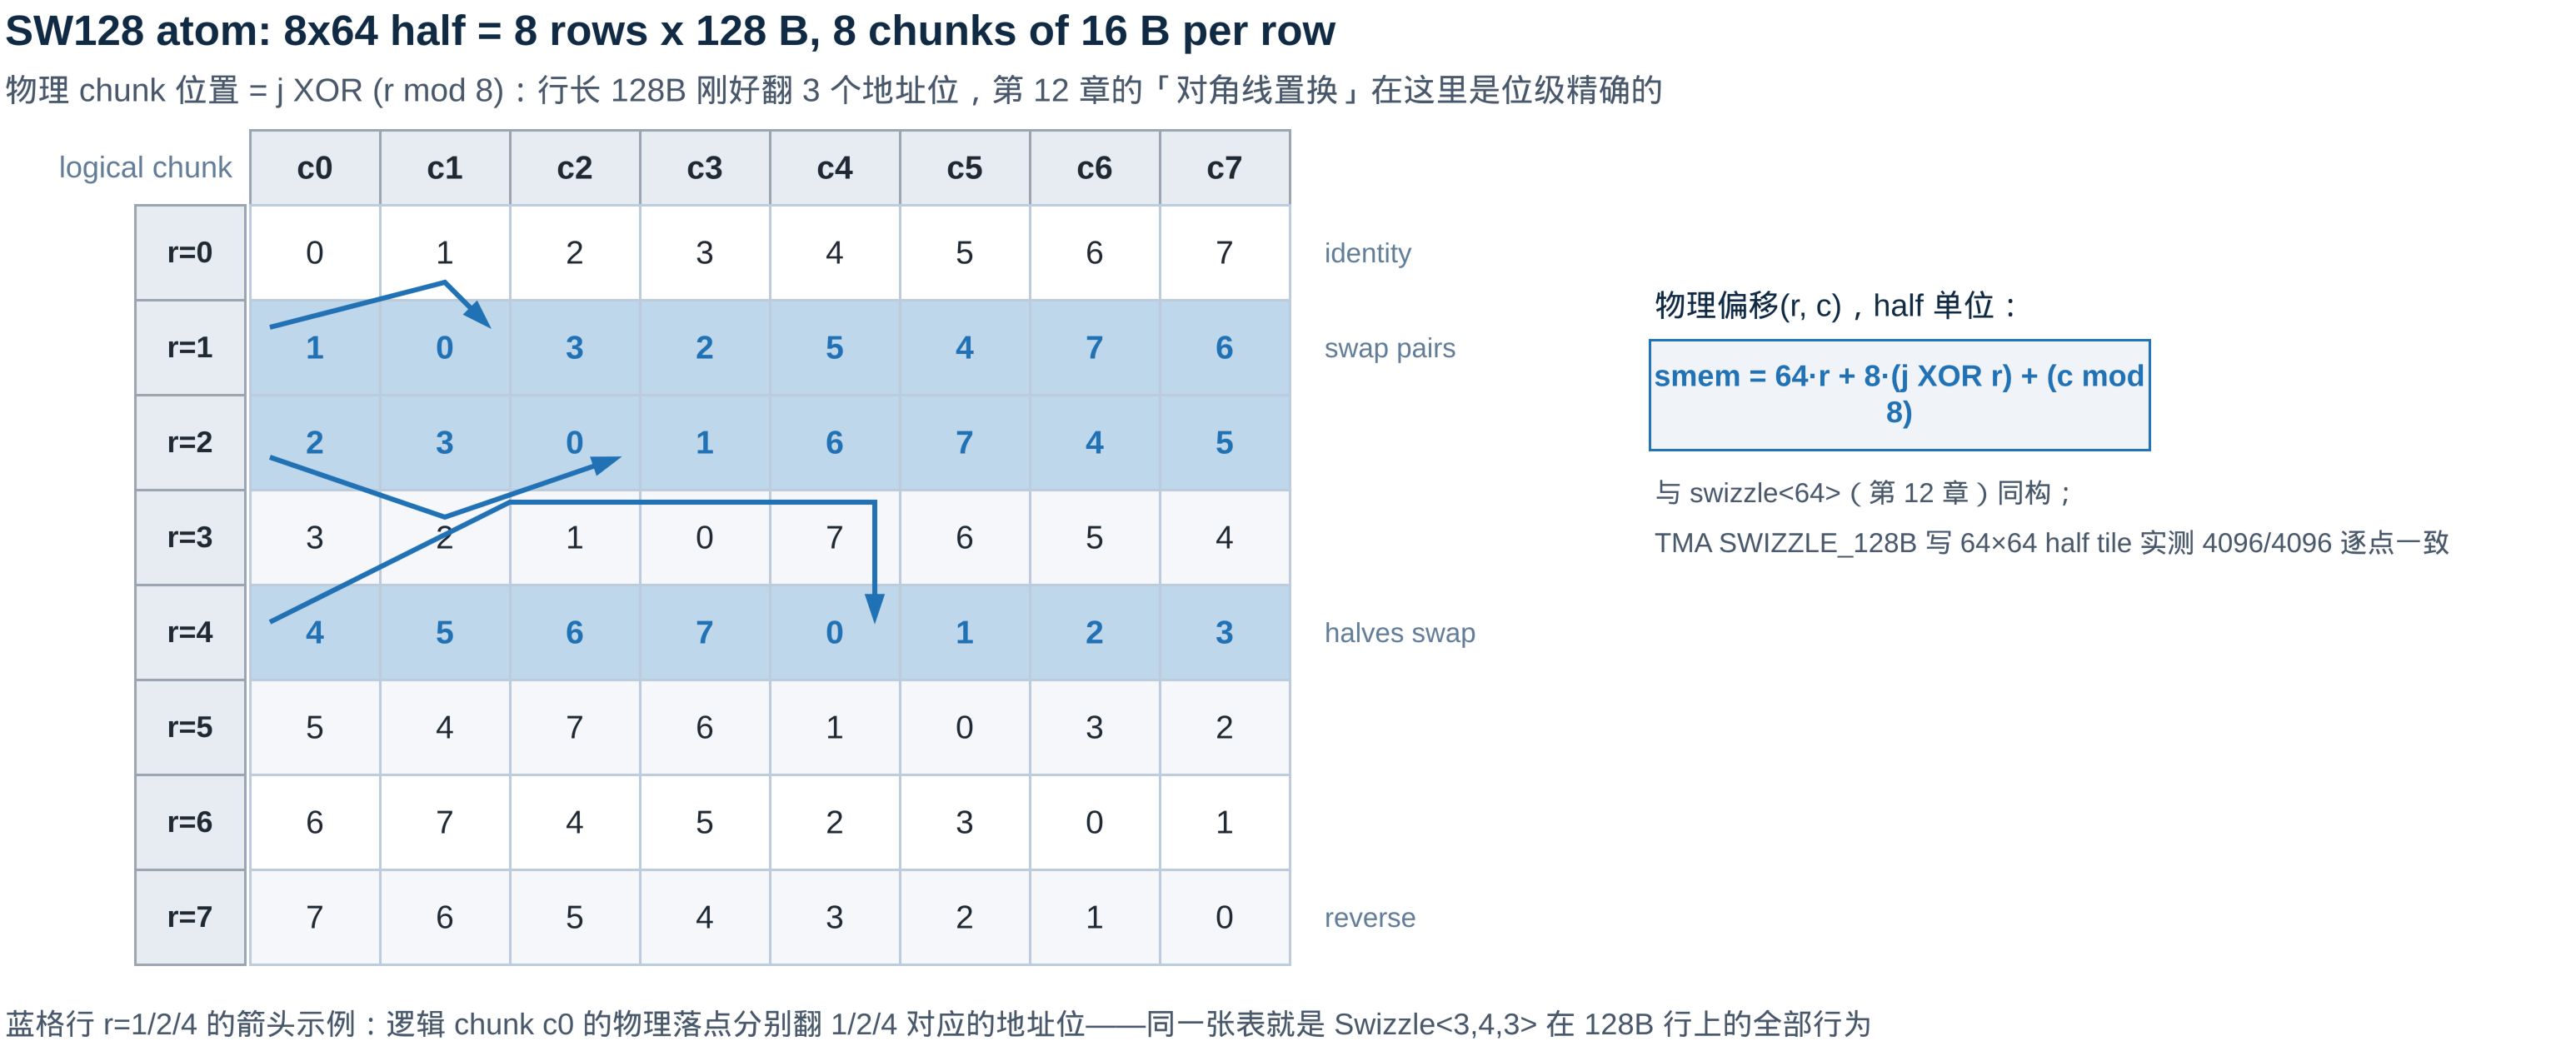
\includegraphics[width=0.9\textwidth]{figures/drawio/fig-23-1-sw128/fig-23-1.png}
\begin{tikzpicture}[font=\tiny, x=0.01525cm, y=-0.01525cm]
  \node[anchor=west, font=\footnotesize\bfseries] at (30,26)
    {SW128 atom: 8$\times$64 half $=$ 8 rows $\times$ 128 B, 8 chunks of 16 B per row};
  \node[anchor=west, font=\scriptsize] at (30,50)
    {物理 chunk 位置 $= j \oplus (r \bmod 8)$：行长 128\,B 刚好翻 3 个地址位，
     第~\ref{ch:12}~章的\textbf{对角线置换}在这里是位级精确的};
  \node[anchor=west, font=\tiny, text=gray!80] at (24,81) {logical chunk};
  \foreach \cc in {0,...,7}{
    \node[draw=gray!45, fill=gray!12, font=\tiny\bfseries, minimum width=0.79cm,
          minimum height=0.46cm, inner sep=0pt] at ({156+52*\cc},81) {c\cc};
  }
  \foreach \rr in {0,...,7}{
    \node[anchor=east, font=\tiny\bfseries, text=gray!80, minimum height=0.58cm]
      at (128,{115+38*\rr}) {r=\rr};
    \foreach \cc in {0,...,7}{
      \pgfmathtruncatemacro{\vv}{int(mod(\cc+\rr,2)) +
        2*int(mod(int(\cc/2)+int(\rr/2),2)) + 4*int(mod(int(\cc/4)+int(\rr/4),2))}
      \ifnum\rr=1
        \node[draw=gray!45, fill=tkFillBlue, text=tkBlue, minimum width=0.79cm,
              minimum height=0.58cm, inner sep=0pt] at ({156+52*\cc},{115+38*\rr}) {\vv};
      \else\ifnum\rr=2
        \node[draw=gray!45, fill=tkFillBlue, text=tkBlue, minimum width=0.79cm,
              minimum height=0.58cm, inner sep=0pt] at ({156+52*\cc},{115+38*\rr}) {\vv};
      \else\ifnum\rr=4
        \node[draw=gray!45, fill=tkFillBlue, text=tkBlue, minimum width=0.79cm,
              minimum height=0.58cm, inner sep=0pt] at ({156+52*\cc},{115+38*\rr}) {\vv};
      \else\ifnum\rr=3
        \node[draw=gray!45, fill=gray!6, minimum width=0.79cm, minimum height=0.58cm,
              inner sep=0pt] at ({156+52*\cc},{115+38*\rr}) {\vv};
      \else\ifnum\rr=5
        \node[draw=gray!45, fill=gray!6, minimum width=0.79cm, minimum height=0.58cm,
              inner sep=0pt] at ({156+52*\cc},{115+38*\rr}) {\vv};
      \else\ifnum\rr=7
        \node[draw=gray!45, fill=gray!6, minimum width=0.79cm, minimum height=0.58cm,
              inner sep=0pt] at ({156+52*\cc},{115+38*\rr}) {\vv};
      \else
        \node[draw=gray!45, fill=white, minimum width=0.79cm, minimum height=0.58cm,
              inner sep=0pt] at ({156+52*\cc},{115+38*\rr}) {\vv};
      \fi\fi\fi\fi\fi\fi
    }
  }
  \node[anchor=west, font=\tiny, text=gray!80] at (558,115) {identity};
  \node[anchor=west, font=\tiny, text=gray!80] at (558,153) {swap pairs};
  \node[anchor=west, font=\tiny, text=gray!80] at (558,267) {halves swap};
  \node[anchor=west, font=\tiny, text=gray!80] at (558,381) {reverse};
  \draw[-{Stealth[length=1.8mm]}, tkBlue, very thick] (138,142) -- (222,142);
  \draw[-{Stealth[length=1.8mm]}, tkBlue, very thick] (138,180) -- (274,180);
  \draw[-{Stealth[length=1.8mm]}, tkBlue, very thick] (138,256) -- (376,256);
  \node[anchor=west, font=\tiny, text=gray!80] at (690,136)
    {物理偏移$(r, c)$，half 单位：};
  \node[anchor=west, draw=tkBlue, fill=tkFillBlue, text=tkBlue, font=\tiny,
        inner sep=3pt] at (690,172)
    {smem $= 64r + 8(j \oplus r) + (c \bmod 8)$};
  \node[anchor=west, font=\tiny] at (690,211)
    {与 \texttt{swizzle<64>}（第~\ref{ch:12}~章）同构；};
  \node[anchor=west, font=\tiny] at (690,231)
    {TMA \texttt{SWIZZLE\_128B} 写 $64\times64$ half tile 实测 $4096/4096$ 逐点一致};
  \node[anchor=west, font=\tiny] at (30,424)
    {蓝格行 $r=1/2/4$ 的箭头示例：逻辑 chunk $c_0$ 的物理落点分别翻 $1/2/4$
     对应的地址位——同一张表就是 \texttt{Swizzle<3,4,3>} 在 128\,B 行上的全部行为};
\end{tikzpicture}
\caption{SW128 原子的物理排布：16\,B 块的列号 XOR 行号。横轴为 8 个
逻辑 chunk（$c_0$--$c_7$），纵轴 8 行，格内为该行接受置换后的物理
chunk 下标；蓝底行 $r=1/2/4$ 给出 chunk $c_0$ 落点翻转 $1/2/4$ 地址位的
示例。物理偏移 $=64r+8\cdot(j\oplus r)+(c\bmod 8)$（half 单位）——与
\texttt{swizzle<64>}（第~\ref{ch:12}~章）同构。}
\label{fig:23-1}
\end{figure}

\begin{figure}[htbp]
\centering
% was: 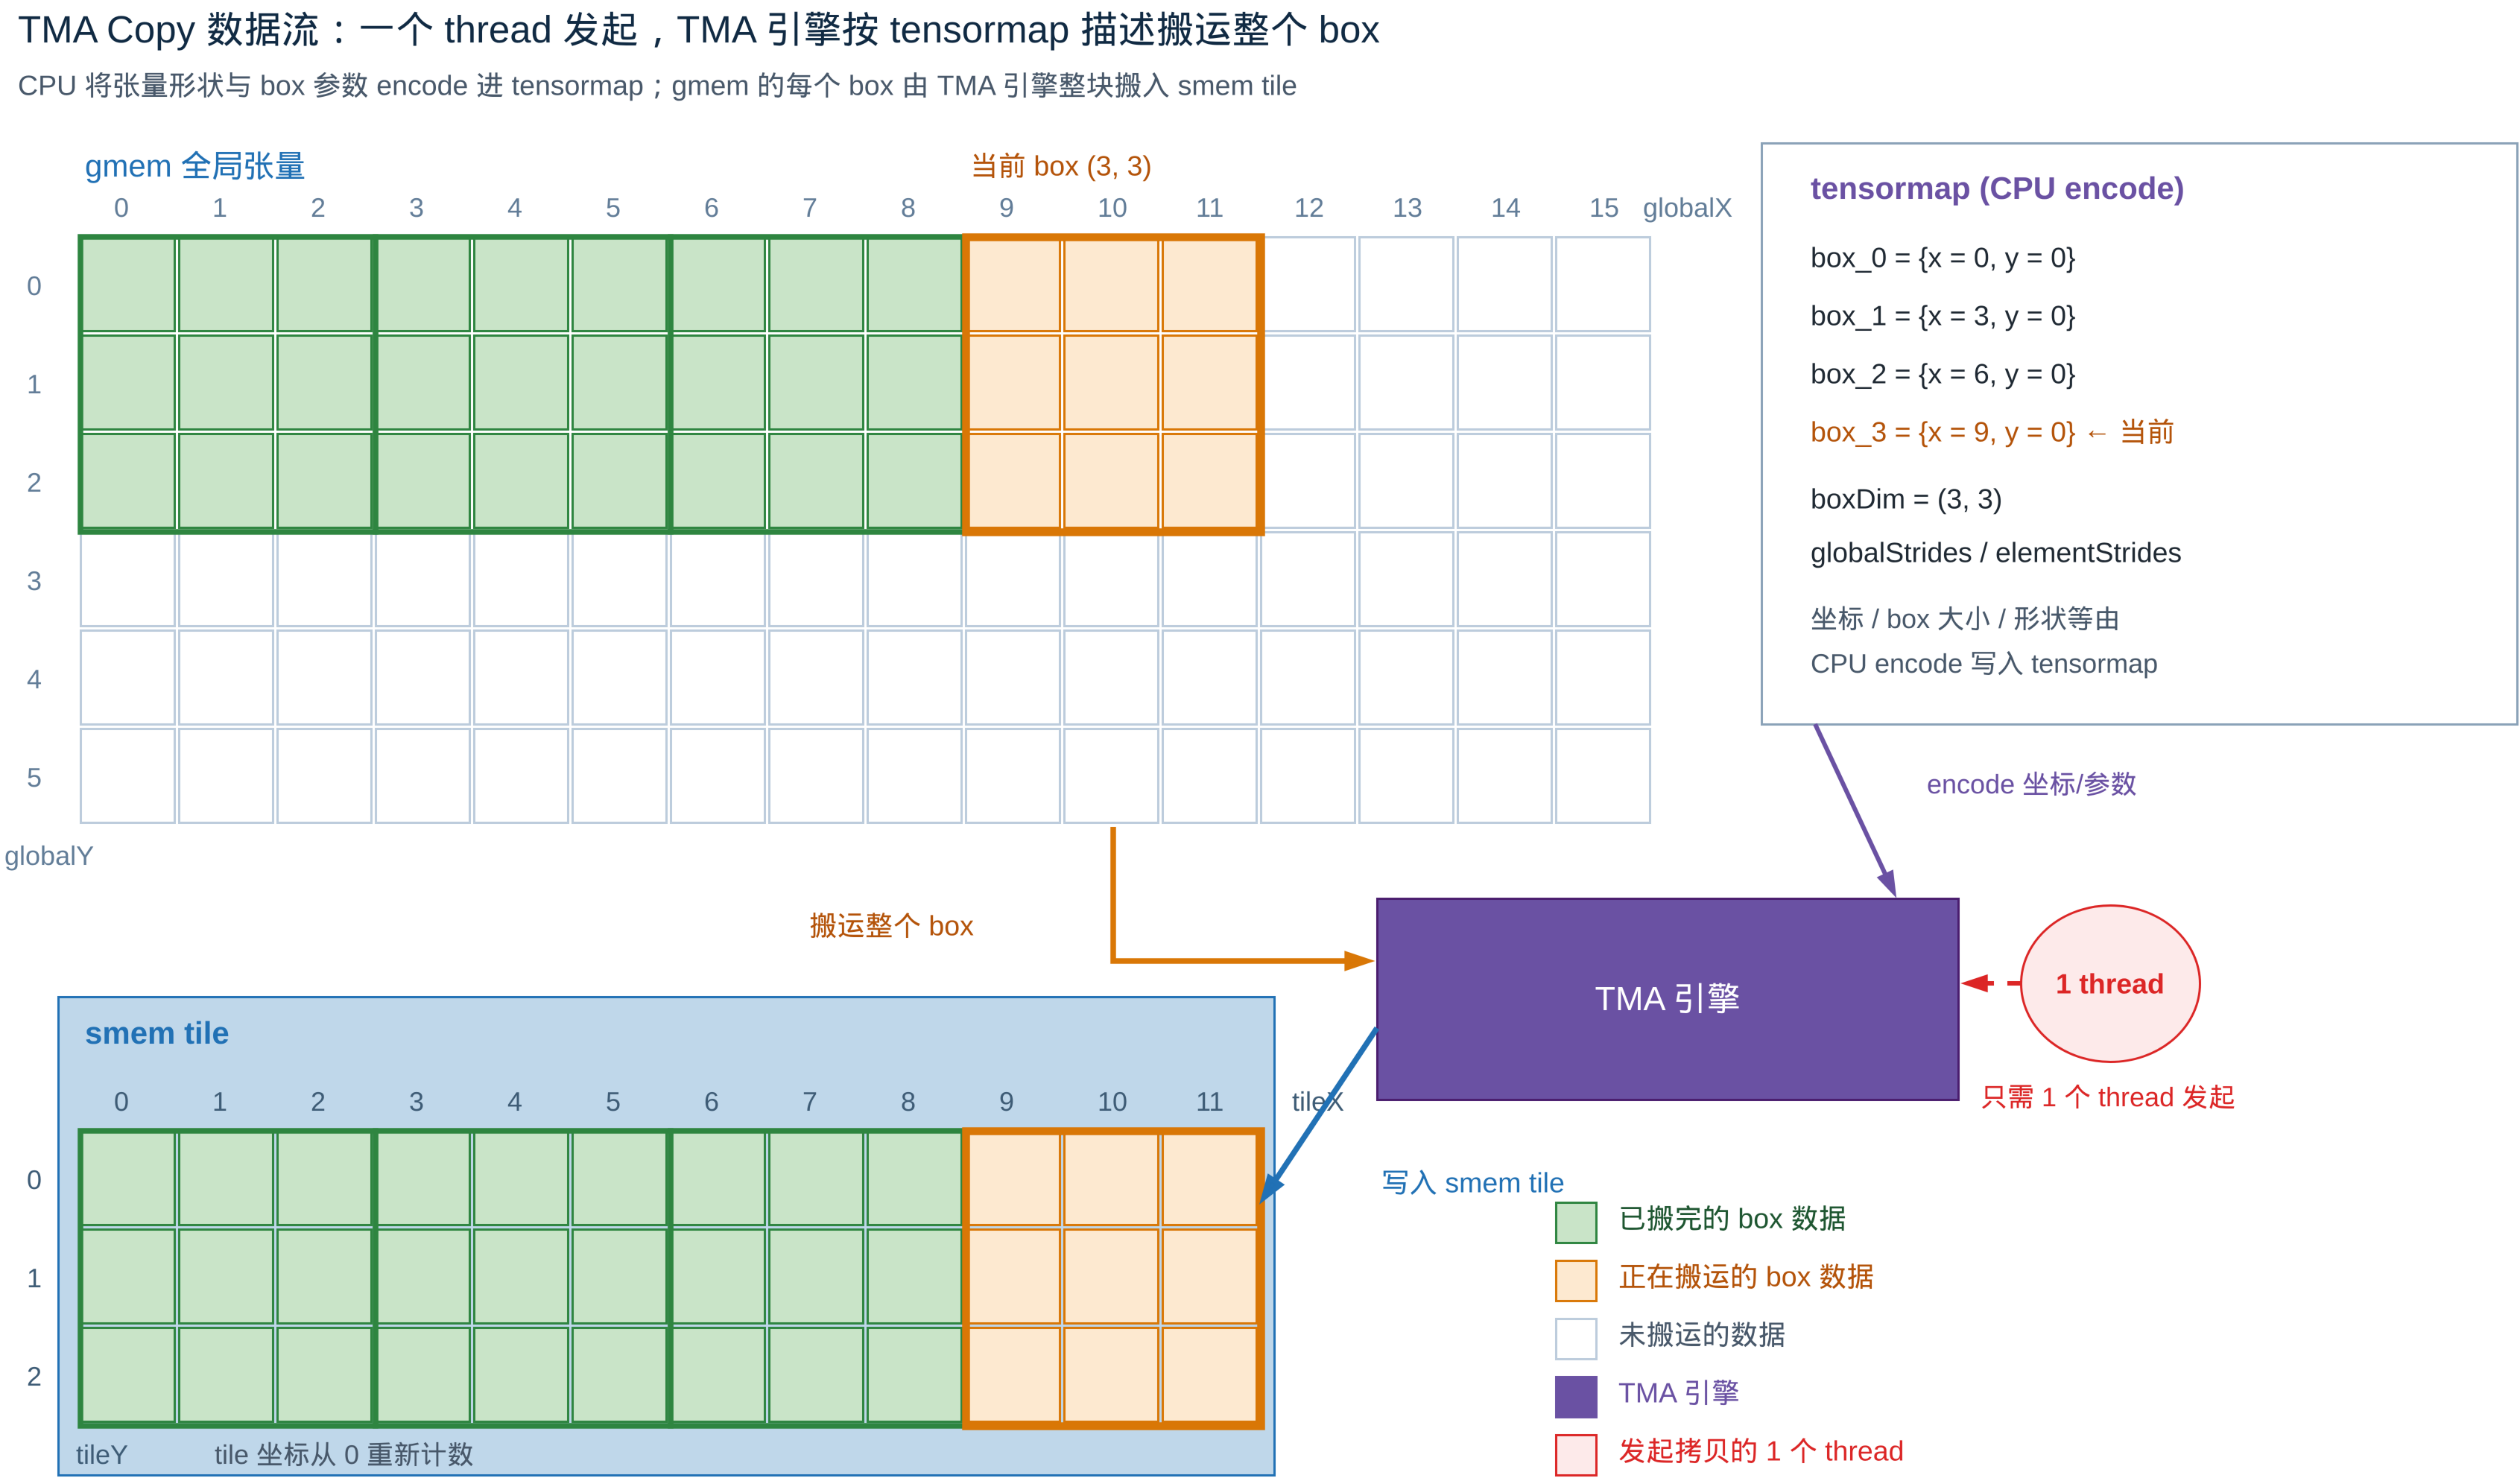
\includegraphics[width=0.95\textwidth]{figures/drawio/fig-23-2-tma-copy-flow/fig-23-2.png}
\begin{tikzpicture}[font=\tiny, x=0.015cm, y=-0.015cm]
  \node[anchor=west, font=\footnotesize\bfseries] at (30,23)
    {TMA Copy 数据流：一个 thread 发起，TMA 引擎按 tensormap 描述搬运整个 box};
  \node[anchor=west, font=\tiny] at (30,48)
    {CPU 将张量形状与 box 参数 encode 进 tensormap；gmem 的每个 box 由 TMA
     引擎整块搬入 smem tile};
  \node[anchor=west, font=\scriptsize, text=tkBlue] at (60,84) {gmem 全局张量};
  \node[anchor=west, font=\tiny, text=tkOrange!80!black] at (456,84)
    {当前 box $(3, 3)$};
  \foreach \cc in {0,...,15}{
    \node[font=\tiny, text=gray!80] at ({82+44*\cc},103) {\cc};
  }
  \foreach \rr in {0,...,5}{
    \node[anchor=east, font=\tiny, text=gray!80] at (52,{138+44*\rr}) {\rr};
    \foreach \cc in {0,...,15}{
      \ifnum\rr<3
        \ifnum\cc<9
          \node[draw=gray!40, fill=tkFillGreen, minimum width=0.63cm, minimum height=0.63cm,
                inner sep=0pt] at ({81+44*\cc},{137+44*\rr}) {};
        \else\ifnum\cc<12
          \node[draw=gray!40, fill=tkFillOrange, minimum width=0.63cm, minimum height=0.63cm,
                inner sep=0pt] at ({81+44*\cc},{137+44*\rr}) {};
        \else
          \node[draw=gray!40, fill=white, minimum width=0.63cm, minimum height=0.63cm,
                inner sep=0pt] at ({81+44*\cc},{137+44*\rr}) {};
        \fi\fi
      \else
        \node[draw=gray!40, fill=white, minimum width=0.63cm, minimum height=0.63cm,
              inner sep=0pt] at ({81+44*\cc},{137+44*\rr}) {};
      \fi
    }
  }
  \draw[tkGreen, very thick] (60,116) rectangle (192,248);
  \draw[tkGreen, very thick] (192,116) rectangle (324,248);
  \draw[tkGreen, very thick] (324,116) rectangle (456,248);
  \draw[tkOrange, very thick] (456,116) rectangle (588,248);
  \node[anchor=west, font=\tiny, text=gray!80] at (746,103) {globalX};
  \node[anchor=west, font=\tiny, text=gray!80] at (24,393) {globalY};
  \node[draw=gray!60, fill=white, minimum width=5.07cm, minimum height=3.9cm,
        inner sep=0pt] at (981,204) {};
  \node[anchor=west, font=\scriptsize, text=tkPurple] at (832,94)
    {tensormap (CPU encode)};
  \foreach \k/\t in {0/{box\_0 $= \{x = 0, y = 0\}$},
                     1/{box\_1 $= \{x = 3, y = 0\}$},
                     2/{box\_2 $= \{x = 6, y = 0\}$}}{
    \node[anchor=west, font=\tiny] at (832,{125+26*\k}) {\t};
  }
  \node[anchor=west, font=\tiny, text=tkOrange!80!black] at (832,203)
    {box\_3 $= \{x = 9, y = 0\}$ $\leftarrow$ 当前};
  \node[anchor=west, font=\tiny] at (832,233) {boxDim $= (3, 3)$};
  \node[anchor=west, font=\tiny] at (832,257) {globalStrides / elementStrides};
  \node[anchor=west, font=\tiny, text=gray!90] at (832,287)
    {坐标 / box 大小 / 形状等由};
  \node[anchor=west, font=\tiny, text=gray!90] at (832,307) {CPU encode 写入 tensormap};
  \node[draw=tkPurple, fill=tkPurple, text=white, font=\scriptsize\bfseries,
        minimum width=3.9cm, minimum height=1.35cm, inner sep=0pt] at (770,457)
    {TMA 引擎};
  \node[draw=tkRed, fill=tkFillRed, text=tkRed, font=\tiny\bfseries,
        minimum width=1.2cm, minimum height=1.05cm, inner sep=0pt] at (968,450)
    {1 thread};
  \node[anchor=west, font=\tiny, text=tkRed] at (908,501) {只需 1 个 thread 发起};
  \node[draw=tkBlue, fill=tkFillBlue, minimum width=8.16cm, minimum height=3.21cm,
        inner sep=0pt] at (322,563) {};
  \node[anchor=west, font=\scriptsize, text=tkBlue] at (60,472) {smem tile};
  \foreach \rr in {0,...,2}{
    \node[anchor=east, font=\tiny, text=gray!90] at (52,{538+44*\rr}) {\rr};
    \foreach \cc in {0,...,11}{
      \ifnum\cc<9
        \node[draw=gray!40, fill=tkFillGreen, minimum width=0.63cm, minimum height=0.63cm,
              inner sep=0pt] at ({81+44*\cc},{537+44*\rr}) {};
      \else
        \node[draw=gray!40, fill=tkFillOrange, minimum width=0.63cm, minimum height=0.63cm,
              inner sep=0pt] at ({81+44*\cc},{537+44*\rr}) {};
      \fi
    }
  }
  \draw[tkGreen, very thick] (60,516) rectangle (192,648);
  \draw[tkGreen, very thick] (192,516) rectangle (324,648);
  \draw[tkGreen, very thick] (324,516) rectangle (456,648);
  \draw[tkOrange, very thick] (456,516) rectangle (588,648);
  \foreach \cc in {0,...,11}{
    \node[font=\tiny, text=gray!90] at ({82+44*\cc},503) {\cc};
  }
  \node[anchor=west, font=\tiny, text=gray!90] at (592,503) {tileX};
  \node[anchor=west, font=\tiny, text=gray!90] at (56,661) {tileY};
  \node[anchor=west, font=\tiny] at (118,661) {tile 坐标从 0 重新计数};
  \draw[-{Stealth[length=2mm]}, tkOrange, very thick] (522,380) -- (522,440) -- (636,440);
  \node[anchor=west, font=\tiny, text=tkOrange!80!black] at (384,424) {搬运整个 box};
  \draw[-{Stealth[length=2mm]}, tkPurple, thick] (836,334) -- (872,409);
  \node[anchor=west, font=\tiny, text=tkPurple] at (884,361) {encode 坐标/参数};
  \draw[-{Stealth[length=2mm]}, tkBlue, very thick] (652,502) -- (588,546);
  \node[anchor=west, font=\tiny, text=tkBlue] at (640,539) {写入 smem tile};
  \draw[-{Stealth[length=2mm]}, tkRed, dashed, thick] (926,450) -- (904,450);
  \foreach \k/\t in {0/{已搬完的 box 数据}, 1/{正在搬运的 box 数据},
                     2/{未搬运的数据}, 3/{TMA 引擎}, 4/{发起拷贝的 1 个 thread}}{
    \ifnum\k=0
      \node[draw=tkGreen!60, fill=tkFillGreen, minimum width=0.27cm, minimum height=0.27cm,
            inner sep=0pt] at (729,{557+26*\k}) {};
    \else\ifnum\k=1
      \node[draw=tkOrange!70, fill=tkFillOrange, minimum width=0.27cm, minimum height=0.27cm,
            inner sep=0pt] at (729,{557+26*\k}) {};
    \else\ifnum\k=2
      \node[draw=gray!40, fill=white, minimum width=0.27cm, minimum height=0.27cm,
            inner sep=0pt] at (729,{557+26*\k}) {};
    \else\ifnum\k=3
      \node[draw=tkPurple, fill=tkPurple, minimum width=0.27cm, minimum height=0.27cm,
            inner sep=0pt] at (729,{557+26*\k}) {};
    \else
      \node[draw=tkRed, fill=tkFillRed, minimum width=0.27cm, minimum height=0.27cm,
            inner sep=0pt] at (729,{557+26*\k}) {};
    \fi\fi\fi\fi
    \node[anchor=west, font=\tiny] at (746,{555+26*\k}) {\t};
  }
\end{tikzpicture}
\caption{TMA copy 数据流：全局张量按 $3\times3$ box 切分（绿=已搬完、橙=搬运中），各 box 起始坐标与张量描述由 CPU encode 进 tensormap，TMA 引擎据此定位整块搬运。发起与搬运分离——单线程发起拷贝指令，box 内全部元素由 TMA 引擎异步搬入 smem；数据落地后改用 tile 局部坐标，与全局坐标脱钩。重建自 @竹熙佳处《写给大家看的 CuTe 教程：TMA Copy》。}
\label{fig:23-2}
\end{figure}

\section{性能分析}

本章没有为 CuTe swizzle 单独建 bench（Phase~7c 的数据由 \texttt{bench/bench\_leetcuda.cu}
的 \texttt{--bench} 统一采集；端到端性能对照见第~\ref{ch:14}、\ref{ch:24}~章）。
这里只给三条可核验的定量结论：

\textbf{(1) bank conflict 的消除是块级的。} 一个 16 B chunk 占 4 个
bank（128 B $=$ 32 个 4 B bank）。式~\eqref{eq:23-chunk} 保证同一列块
（固定 $j$）在 8 行里落到 8 个互不相同的物理 chunk，即 8 个 4-bank
组，这正好是 \texttt{ldmatrix}（每线程取 16 B）所需要的性质。第
\ref{sec:23-minitest}~节的 case C 把它写成固定 chunk、行扫描得 8 个
不同值，case F 则验证 $8\times32$ 原子的退化形态
（\texttt{chunk'} $=$ \texttt{chunk} $\oplus$ $(\text{row}\gg1)$，
XOR 值只有 $\{0,8,16,24\}$ 四种，相邻两行共享图样，8 行一周期）。

\textbf{(2) swizzle 不需要独立的数据重排指令。} 软件
\texttt{ldmatrix} 路径把 XOR 折叠进地址表达式，SASS 里可能多出一条
\texttt{LOP3} 或少量整数指令；TMA 路径则由 descriptor 让硬件完成相应模式。
因此应说“没有额外的数据搬运指令”，而不是“零条额外指令”。

\textbf{(3) TMA 的收益不在拷贝更快，而在同步与数据管理更简单。} 生产者
只有 1 个线程发指令（式~\eqref{eq:23-tx} 的字节数由硬件事务计数保证），
256 个线程不再参与 G$\to$S 的地址计算，也不再需要
\texttt{\_\allowbreak{}\_\allowbreak{}syncthreads}，hgemm.cuh~L1990--2012 的注释把这一点总结为
\textbf{barrier $+$ proxy fence 取代了 CTA 级同步}。对本章而言，快是
次要的；谁算地址、谁保证一致这两个问题的答案变得唯一，
才是 TMA 对 kernel 工程的主要贡献。

\begin{equation}
\label{eq:23-tx}
N_{\text{tx}} = (B_M\!\cdot\!B_K + B_N\!\cdot\!B_K)\times
\texttt{sizeof\allowbreak{}(half)} = (128\!\cdot\!64+128\!\cdot\!64)\times2 = 32768\ \text{B}.
\end{equation}

\section{常见坑}

\begin{enumerate}[leftmargin=2.2em]
\item \textbf{拿复合布局当偏移公式。} 带 swizzle 的
\texttt{Composed\allowbreak{}Layout} 求值是位置无关的，TMA 硬件是位置相关的：
同一个逻辑坐标在两个语义下可以指向不同物理地址。要么全用布局
（\texttt{make\_tensor}/\texttt{Tensor}），要么全用公式（第~\ref{ch:12}~章的
\texttt{swizzle<>}），混用必错。
\item \textbf{基址对齐不够。} 本章经典 TMA 三档的 smem 基址要求分别为：
32\,B swizzle 对齐 256\,B，64\,B 对齐 512\,B，128\,B 对齐 1024\,B。
不能把 WGMMA descriptor 的对齐要求套到 TMA；\texttt{ldmatrix} 本身
也没有 1024\,B 这一硬件对齐规则，它只消费软件算出的 lane 地址。
\item \textbf{把 $M$ 当成元素粒度。} $2^M$ 是\emph{基本块}的字节数
（16\,B $=2^4$），不是元素个数；fp32 里它等于 4 个元素，fp16 里等于
8 个元素。经典三档使用 $M=4$，但 128\,B 模式还有受版本和架构约束的
$M=5/6$ 原子粒度变体，不能泛称 descriptor 只接受 $M=4$。
\item \textbf{\texttt{tile\_\allowbreak{}to\_\allowbreak{}shape} 不整除。} $8\times64$ 原子铺
$B_K=32$ 会直接断言失败；要么换原子，要么改 tile 形状。
\item \textbf{把 \texttt{k\_step} 加在 swizzle 外部。} 只要 slice 宽度
不是 swizzle 周期的整数倍，偏移就必须放进 swizzle 内部
（hgemm.cuh~L2021--2034 的注释），否则某些 $k_{\text{step}}$ 的
chunk 会跨 slice 交叉。
\item \textbf{预期 swizzle 能消除所有 bank conflict。} 它保证的是
\textbf{同一个 16 B 块列在 8 行内落到 8 个不同块}；跨 32 行、或以
4 B 为粒度的模式（例如标量表查）它不保证。强度由 $B$ 与行宽共同决定：
hgemm 路径的 $8\times32$ 原子实际强度只有 2 bit（4 个 XOR 图样，
相邻两行共享图样、8 行一周期，4.1 节实践须知）。
\item \textbf{忘记 swizzle 是地址函数。} 想让按 (\texttt{row,col}) 求值
的布局与按 flat 偏移求值的公式一致，前提是行宽恰好等于
$2^{M+S}$ 字节。行宽不匹配时（例如 $B_K$ 取 48），两者不等。
\end{enumerate}

\section{面试要点速查}

\textbf{Q1：\texttt{Swizzle\allowbreak{}<B,\allowbreak{}M,\allowbreak{}S>} 的三个参数各是什么？}
$M$：被保留的连续低位位数（基本块宽 $2^M$ 字节）；$B$：XOR 掩码位数，
同时决定 TMA 模式名（32/64/128\,B $\leftrightarrow$ 1/2/3）。
$S$：\texttt{YYY} 相对 \texttt{ZZZ} 的位移；仅当行宽恰好为 $2^{M+S}$
字节时（三档中只有 SW128 满足，见 Q2）才等价于一行 $2^{M+S}$ 字节，
工程上恒取 3。约束 $|S|\ge B$。

\textbf{Q2：为什么 $S$ 恒为 3？} 三档的 XOR 源字段固定取自 bit~7
（128\,B 粒度）、目标字段固定取自 bit~4（16\,B 块），两者相距 3 位，
故字节口径下 $S$ 恒为 3、$M$ 恒为 4（与 dtype 无关）；档间只改 $B$
（1/2/3）与 box 内维（行宽 32/64/128\,B）。fp16 元素口径下 $M=3$
（hgemm 自用的 \texttt{Swizzle\allowbreak{}<3,\allowbreak{}3,\allowbreak{}3>} 即此口径）。

\textbf{Q3：为什么不直接写成列块 XOR 行号，还要用位运算？}
因为 TMA 与 WGMMA descriptor 用字节地址上的位域模式描述硬件行为；
列块 XOR 行号只有在行宽 $=2^{M+S}$ 时才与位公式等价
（式~\eqref{eq:23-chunk}）。\texttt{ldmatrix} 不执行 descriptor swizzle，
它只是接收软件已经算好的 lane 地址，因此软件也必须用同一套位公式。

\textbf{Q4：\texttt{composition} 的求值顺序？} 先算基础布局得偏移，
Swizzle 再作用其上：$R(c)=\text{Swizzle}(\text{Layout}(c))$。
Swizzle 不参与坐标分解。

\textbf{Q5：TMA swizzle 与手写 swizzle 的冲突点在哪？} 在相位。
TMA 硬件按绝对地址和 descriptor 模式算 phase，软件按相对偏移算；基址
必须满足所选模式的对齐要求：经典 32/64/128\,B 三档分别为
256/512/1024\,B。WGMMA 有 \texttt{base\_offset} 字段可以补偿；
\texttt{ldmatrix} 没有这个字段，只能由软件地址计算保证一致。

\textbf{Q6：给定 $B_K$ 与 fp16，怎么判断该用哪种 swizzle？} 先算行宽
$B_K\times2$ 字节；可选行宽 32/64/128\,B，要求 $B_K\times2\ge$
模式行宽且 $16$\,B 块宽整除行宽。$B_K=64$ 时行宽 128\,B
$\Rightarrow$ \texttt{Swizzle\allowbreak{}<3,\allowbreak{}4,\allowbreak{}3>}（字节）或 \texttt{Swizzle\allowbreak{}<3,\allowbreak{}3,\allowbreak{}3>}
（元素）；$B_K=32$ 时行宽 64\,B，只能退到 64\,B 或更弱的模式。

\section{最小测试与动手实验}\label{sec:23-minitest}

\texttt{book/\allowbreak{}tests/\allowbreak{}ch23\_\allowbreak{}swizzle\_\allowbreak{}tma.cu} 是一个主机侧断言程序
（需要 \texttt{NOTES\_\allowbreak{}V2\_\allowbreak{}ENABLE\_\allowbreak{}CUTE}），它把本章的公式逐条与 CuTe 的
布局求值结果对照，不启动任何 kernel。七个 case：

\begin{enumerate}[leftmargin=2.2em]
\item \textbf{case A}：\texttt{Swizzle\allowbreak{}<3,\allowbreak{}3,\allowbreak{}3>} 的位级公式：对
$[0,1024)$ 内每个字节偏移验证 $\text{apply}(\text{off})=\text{off}\oplus
((\text{off}\wedge(\texttt{0b111}\ll6))\gg3)$，并核对
\texttt{yyy\_msk}/\texttt{zzz\_msk} 常量、统计 $8$ 个 \texttt{YYY} 值与
$8$ 个 chunk 各被覆盖 $128$ 次；
\item \textbf{case B}：对合性 $\text{apply}(\text{apply}(x))=x$ 与
$[0,512)$ 上的双射，再用自定义 base layout
$\texttt{\allowbreak{}(8,\allowbreak{}8):\allowbreak{}(64,\allowbreak{}8)}$（64\,B 行、8\,B 块）验证
$R(r,c)=64r+8\cdot(c\oplus r)$，并检查固定块列扫 $8$ 行得到 $8$ 个
不同物理块、$8$ 个不同 bank；
\item \textbf{case C}：把字节空间的 \texttt{Swizzle\allowbreak{}<3,\allowbreak{}4,\allowbreak{}3>}（即
\texttt{make\_tensor} 后指针路径的位置相关语义）作用在
\texttt{GMMA::\allowbreak{}Layout\_\allowbreak{}K\_\allowbreak{}SW128\_\allowbreak{}Atom\allowbreak{}<half>} 的 $8\times64$ 域上，
$512$ 个坐标全部满足式~\eqref{eq:23-chunk}；
\item \textbf{case D}：\texttt{composition} 语义
$R(c)=\text{Swizzle}(\text{Base}(c))$，两种 base layout 各遍历全
domain（$256+256$ 个坐标）；
\item \textbf{case E}：硬件对照：sm\_120a 实测的 TMA
\texttt{SWIZZLE\_\allowbreak{}128\allowbreak{}B} $8\times8$ chunk 掩码表（$64$ 槽）与
\texttt{Swizzle\allowbreak{}<3,\allowbreak{}4,\allowbreak{}3>} 逐槽比较，再由该表导出 $4096$ 点排布逐点比较；
同时统计 \texttt{tile\_\allowbreak{}to\_\allowbreak{}shape} 分块布局\emph{裸求值}的命中数
（$1024/4096$），用于说明把字节口径 swizzle 直接套在元素偏移上的
单位错配（补上 $\times2$ recast 后应 $4096/4096$）；
\item \textbf{case F}：$8\times32$ 原子的退化形态（4.1 节实践须知）：
验证 $\text{chunk}'=\text{chunk}\oplus(\text{row}\gg1)$，XOR 值集合为
$\{0,8,16,24\}$、每个值覆盖 $2$ 行（$=64$ 个坐标）；
\item \textbf{case G}：TMA 编译级核对：\texttt{Tma\allowbreak{}Descriptor}
$=$ \texttt{CUtensorMap} 且尺寸为 $128$\,B、三档掩码常量、SW128 atom 的
\texttt{layout\_a()}/\texttt{layout\_b()} 类型与其 \texttt{shape}/
\texttt{stride}/cosize，以及在 host 侧用 \texttt{make\_\allowbreak{}tma\_\allowbreak{}copy}
真正构造出一个 descriptor 并核对 (gmem 张量, CTA tile) 的
size/stride 推导。
\end{enumerate}

编译与运行：

\begin{lstlisting}[style=console]
  cd book/tests
  ./build_tests.sh --arch sm_120a --ch ch23
\end{lstlisting}

预期输出（$2026$-$09$-$11$ 于 RTX PRO 5000 / sm\_120a 实机执行，全文）：

\begin{lstlisting}[style=console]
== ch23 CuTe swizzle / TMA (host-side assertions) ==
PASS case A Swizzle<3,3,3> bit formula: mismatches=0 (1044 checks)
PASS case B involution + bijection + base layout: mismatches=0 (1105 checks)
PASS case C byte-space Sw<3,4,3> == chunk XOR row: mismatches=0 (576 checks)
PASS case D composition R(c) == Swizzle(Base(c)): mismatches=0 (512 checks)
      (E) measured table mismatches=0
      (E) 4096-point mismatches=0, tiled formula 1024/4096
PASS case E hardware SWIZZLE_128B cross-check: mismatches=0 (3 checks)
PASS case F hgemm 8x32 atom effective swizzle: mismatches=0 (262 checks)
PASS case G TMA compile-level (descriptor): mismatches=0 (15 checks)
ALL OK
\end{lstlisting}
（\texttt{tiled formula 1024/4096} 一行是裸求值（字节口径 swizzle 直接
作用在元素偏移上）的口径错配结果，补上 $\times2$ recast 后为
$4096/4096$。\texttt{build\_\allowbreak{}tests.\allowbreak{}sh} 在该输出之后还会再打印一次
\texttt{ALL OK} 作为汇总，退出码 $0$。）

动手实验（可选）：把 case F 里的 \texttt{Swizzle\allowbreak{}<3,\allowbreak{}3,\allowbreak{}3>} 换成
\texttt{Swizzle\allowbreak{}<3,\allowbreak{}4,\allowbreak{}3>}（相当于把 $8\times32$ 原子按 128\,B 行宽去解释），
重跑并打印 XOR 值集合。两次结果的差异正是 4.1/3.3 节实践须知要读者亲手
复现的那一步：\textbf{同一个 \texttt{Swizzle} 类型在不同 base layout 下的
物理效果不同，参数必须与行宽一起读}。

\section*{延伸阅读}

\begin{itemize}[leftmargin=1.6em]
\item @reed，\emph{cute 之 Swizzle}（ch12/23 主参考）：
\url{https://zhuanlan.zhihu.com/p/671419093}
\item @reed，\emph{cute 之 TMA Descriptor 编码与隐藏的第 21bit}
（descriptor 字段与 swizzle 模式编码）：
\url{https://zhuanlan.zhihu.com/p/2037200219700449995}
\item @竹熙佳处，\emph{CuTe 教程：TMA Copy}（\texttt{make\_\allowbreak{}tma\_\allowbreak{}copy}
的用法与边界）：
\url{https://zhuanlan.zhihu.com/p/2003198909405763007}
\item @weishengying，\emph{cute swizzle}（可运行的最小例子）：
\url{https://zhuanlan.zhihu.com/p/706796240}
\item @Anonymous，\emph{GEMM 细节分析（三）：Swizzle<B,M,S> 参数取值}
（三个档位的参数对照）：\url{https://zhuanlan.zhihu.com/p/713713957}
\end{itemize}

% ch24-cute-hgemm.tex — CuTe 应用（一）：HGEMM（RFC-F，2026-09-11）
% \url 由 book.tex 的 hyperref 提供；单章独立编译时降级为可断行的 \ttfamily
% （逐字符插入 \allowbreak，避免长 URL 造成 Overfull \hbox）
\makeatletter
\providecommand{\urlchbrk}[1]{\@tfor\next:=#1\do{\next\allowbreak}}
\makeatother
\providecommand{\url}[1]{{\ttfamily\urlchbrk{#1}}}
\chapter{CuTe 应用（一）：HGEMM}\label{ch:24}

\section{本章导读}

第~\ref{ch:11}、\ref{ch:12}~章用两条不同的路把同一个 HGEMM 写了两遍：一条是
手写 MMA PTX $+$ 手算 smem 地址的 Phase~7b，另一条是手写 XOR swizzle $+$
寄存器双缓冲的 Phase~7b-3。Phase~7b-3 跑到了 122.9\,TFLOPS
（2048$\times$16384），Phase~7b 为 76.55\,TFLOPS（1024$^3$），但代价是同一组
形状与步长的事实被反复重写：\texttt{ldmatrix} 的 lane 映射、swizzle 的
XOR 掩码、epilogue 的 \texttt{\_\_shfl\_sync} 编排，每一处都要人工保证与其余
四处的地址算术一致。本章把同一个 kernel 交给 CuTe 重写一遍，用的是 Phase~7c 的
\texttt{hgemm\_\allowbreak{}mma\_\allowbreak{}stages\_\allowbreak{}tn\_\allowbreak{}cute}，并在最后用一张对照表
（图~\ref{fig:24-1}）把两条路逐项摆开。

\textbf{前置章节}：第~\ref{ch:11}~章（\texttt{mma.\allowbreak{}sync.\allowbreak{}m16n8k16} 与
\texttt{ldmatrix}）、第~\ref{ch:12}~章（XOR swizzle 与寄存器双缓冲）、
第~\ref{ch:20}--\ref{ch:23}~章（Layout 代数 / Tensor 与 TiledCopy / TiledMMA /
Swizzle 与 TMA）。本章是 Part~IV 的第一章\textbf{应用篇}，只用到前四章已经介绍过的
四个抽象：\texttt{Layout}、\texttt{Tensor}、\texttt{TiledCopy}、
\texttt{TiledMMA}。

\textbf{阅读路线}：本章沿 @reed 的 CuTe GEMM 三部曲《cute 之 简单 GEMM
实现》《cute 之 GEMM 流水线》《cute 之 高效 GEMM 实现》（链接见文末
\textbf{延伸阅读}）的叙述顺序，按先跑通 $\to$ 再重叠 $\to$ 后提速三步渐进展开。
每一步开头先说明上一版留下了什么问题，再给出这一版的代码，以及读者必须
自己守住的约束。凡是源码注释与实现不一致、或表述容易被误读的地方，不再集中
堆在章末的勘误节，而是就地写成\textbf{实践须知}：这类提醒出现在使用现场比
事后查表更有用。

\textbf{源码区间}：hgemm.cuh~L718--1427：Phase~7c 头注释（L718--778）、
宏块 \texttt{NOTES\_\allowbreak{}V2\_\allowbreak{}ENABLE\_\allowbreak{}CUTE}（L779--1427）内的 kernel
\texttt{hgemm\_\allowbreak{}mma\_\allowbreak{}stages\_\allowbreak{}tn\_\allowbreak{}cute}（L821 起）与 launch wrapper
\texttt{launch\_\allowbreak{}hgemm\_\allowbreak{}mma\_\allowbreak{}stages\_\allowbreak{}tn\_\allowbreak{}cute}（L1216 起）。\textbf{编译宏}：
\texttt{NOTES\_\allowbreak{}V2\_\allowbreak{}ENABLE\_\allowbreak{}CUTE}（需要 CUTLASS 头文件；sm80 及以上均可编）。
\textbf{架构}：本章 kernel 只用 SM80 时代的 \texttt{cp.async} $+$
\texttt{mma.sync} $+$ \texttt{ldmatrix}，本机 sm\_120a 可实测。

配套最小测试 \texttt{book/\allowbreak{}tests/\allowbreak{}ch24\_\allowbreak{}hgemm\_\allowbreak{}cute.cu}：两组配置
（\texttt{k\allowbreak{}Acc\allowbreak{}F32=\allowbreak{}false}、$B_N=256$ 与 \texttt{k\allowbreak{}Acc\allowbreak{}F32=\allowbreak{}true}、$B_N=128$）对 CPU
fp64 参考做正确性判定；本章的实测数字全部来自该测试与 \texttt{ptxas -v}，
端到端性能对照见第~\ref{sec:ch24-perf}~节。

\section{问题与动机}

先把第~\ref{ch:11}、\ref{ch:12}~章的代码量摆出来（只统计代码行，去掉纯注释
与空行；统计口径见第~\ref{sec:24-minitest}~节）：

\begin{itemize}
  \item Phase~7b \texttt{hgemm\_\allowbreak{}mma\_\allowbreak{}stages\_\allowbreak{}tn}（hgemm.cuh~L129--397）：
        151 行；
  \item Phase~7b-3 \texttt{hgemm\_\allowbreak{}mma\_\allowbreak{}stages\_\allowbreak{}tn\_\allowbreak{}swizzle}
        （hgemm.cuh~L434--716）：235 行；
  \item Phase~7c \texttt{hgemm\_\allowbreak{}mma\_\allowbreak{}stages\_\allowbreak{}tn\_\allowbreak{}cute}
        （hgemm.cuh~L821--1196）：118 行，再加 launch wrapper
        （L1216--1427）86 行。
\end{itemize}

手写版与 CuTe 版的行数比并不悬殊（235 对 204），但代码的性质变了。
手写版里出现的是地址表达式与内联 PTX：

\begin{lstlisting}
int lane_smem_a_m = warp_m * (kMmaM * kValTileM) + i * kMmaM + lane_id % 16;
int lane_smem_a_k = k_step * kMmaK + (lane_id / 16) * 8;
uint32_t lane_smem_a_ptr = smem_a_base_ptr +
    (stage * BM * BK + lane_smem_a_m * BK +
     swizzle<64>(lane_smem_a_m, lane_smem_a_k)) * sizeof(half);
LDMATRIX_X4(RA[i][0], RA[i][1], RA[i][2], RA[i][3], lane_smem_a_ptr);
\end{lstlisting}

CuTe 版里出现的是声明与分区：

\begin{lstlisting}
auto sA = make_tensor(make_smem_ptr(Ashm), SmemLayoutA{});
auto tAsA = s2r_thr_copy_a.partition_S(sA);
auto tCrA_view = s2r_thr_copy_a.retile_D(tCrA);
cute::copy(s2r_tiled_copy_a, tAsA(_, _, k_step_next, ismem_read),
           tCrA_view(_, _, k_step_next));
\end{lstlisting}

前者把 \texttt{lane} 到 smem 地址的公式写死在 kernel 里，改一个 tile 尺寸就
要把公式推倒重来；后者把同一件事表达成两句声明：\texttt{sA} 的布局是
\texttt{SmemLayoutA}，\texttt{s2r\_\allowbreak{}thr\_\allowbreak{}copy\_\allowbreak{}a} 把 sA 按线程切分。
地址算术由编译器（类型系统）展开，这是第~\ref{ch:20}--\ref{ch:23}~章铺垫四章
换来的东西：把布局从代码里提出来，变成一等公民。

本章要回答三个问题：这 118 行的 kernel 本体做了什么？launch wrapper 的 86 行
类型实例化在配置什么？哪些东西 CuTe 替你做了，哪些仍要你自己做？第三个问题
决定这套工具的能力边界，也是图~\ref{fig:24-1} 要回答的。

正文按三步渐进展开，三步共用同一份源码事实，区别只在每一步放弃或引入什么。

\section{数学原理}

\subsection{问题定义：TN 约定与第一个 Tensor}

本章沿用第~\ref{ch:11}~章的 TN 约定：
$C[M,N] = A[M,K]\times B^{\mathsf T}[N,K]$，其中 $A$、$B^{\mathsf T}$ 都是
row-major（\texttt{A[m][k]}、\texttt{Bt[n][k]}）。写成求和形式：

\begin{equation}
  C_{m,n} \;=\; \sum_{k=0}^{K-1} A_{m,k}\, B_{n,k},
  \label{eq:24-tn}
\end{equation}

注意式~\eqref{eq:24-tn} 里 $B$ 的索引是 $(n,k)$，这就是 TN 的含义：MMA 指令
\texttt{mma.\allowbreak{}sync.\allowbreak{}aligned.\allowbreak{}m16n8k16.row.\allowbreak{}col} 要求 A 为 row-major、B 在 GEMM
语义下为 col-major，而 col-major 的 $B[K,N]$ 与 row-major 的
$B^{\mathsf T}[N,K]$ 是同一块内存。这是本章第一个坑：调用方必须自己把 $B$
转置后传入（最小测试里由 host 侧转置完成，见第~\ref{sec:24-minitest}~节）。

用 CuTe 的话说，TN 是一句关于步长的声明，而不是标志位：

\begin{lstlisting}
  Tensor A = make_tensor(make_gmem_ptr(Aptr), make_shape(m, k),
                         make_stride(k, Int<1>{}));  // A 是 (M,K)，K 连续
  Tensor B = make_tensor(make_gmem_ptr(Bptr), make_shape(n, k),
                         make_stride(k, Int<1>{}));  // Bt 是 (N,K)，K 连续
\end{lstlisting}

两行 \texttt{make\_tensor} 之后，后续所有分区与拷贝都在\textbf{$(shape,stride)$
就是布局}这条约定上工作：$K$ 维连续意味着按 $K$ 切出来的片天然适合做
\texttt{cp.async} 的宽拷贝，而 \texttt{Int<1>\{\}} 这个编译期常量会让
后面每一步的地址算术都在编译期折叠掉。

\subsection{Tile 金字塔：从 CTA tile 到 MMA atom}

一个 CTA 只负责 $C$ 的一小块，整张 $C$ 由网格铺满；$K$ 方向则切开累加
（sliced-K 模式，第~\ref{ch:09}~章）：设 CTA 级 tile 为
$B_M\times B_N\times B_K$，网格为
$\bigl(\lceil N/B_N\rceil,\lceil M/B_M\rceil\bigr)$。Phase~7c 的默认配置：

\begin{equation}
  B_M=128,\qquad
  B_N=\begin{cases}256, & \text{F16 累加}\\ 128, & \text{F32 累加}\end{cases},
  \qquad B_K=32,\qquad k_{\mathrm{stage}}=2 .
  \label{eq:24-tile}
\end{equation}

这三个数字构成一座三层金字塔：CTA tile $B_M\times B_N$（一次搬进来、一次算完）
$\supset$ 逻辑 MMA tile $32\times32\times16$（\texttt{TiledMMA} 一次展开多少条
指令，见下节）$\supset$ atom $16\times8\times16$（一条 \texttt{mma.sync}）。
CuTe 的层层 partition 就是在这座金字塔上做从塔基切到塔尖的坐标换算。三层之间
的尺寸关系见图~\ref{fig:24-tile-pyramid}。

\begin{figure}[H]
\centering
\begin{tikzpicture}[font=\tiny]
  \foreach \gr in {0,...,3}{
    \foreach \gc in {0,...,7}{
      \node[fill=gray!22, minimum width=0.5cm, minimum height=0.5cm, inner sep=0pt]
        at ({\gc*0.5+0.25},{-\gr*0.5-0.25}) {};
    }
  }
  \node[fill=tkOrange!30, draw=tkOrange!80!black, thin, minimum width=0.5cm, minimum height=0.5cm, inner sep=0pt]
    at (3.75,-0.75) {};
  \draw[thin] (0,0) grid[xstep=0.5cm, ystep=0.5cm] (4.0,-2.0);
  \draw[very thick] (0,0) rectangle (4.0,-2.0);
  \node[anchor=south, align=center, font=\scriptsize\bfseries, text width=4.0cm]
    at (2.0,0.12) {CTA tile\\ $B_M\times B_N=128\times256$};
  \node[anchor=north, align=center, text width=4.6cm] at (2.0,-2.1)
    {灰块 $=$ 一个 $32\times32$ MMA tile（$4\times8$ 个铺满整块）};
  \draw[->, very thick] (4.25,-0.75) -- (5.1,-0.75);
  \node[anchor=south] at (4.65,-0.72) {取 1 个};
  \begin{scope}[shift={(5.2,0)}]
    \foreach \wr in {0,...,1}{
      \foreach \wc in {0,...,1}{
        \pgfmathtruncatemacro{\wg}{2*\wr+\wc}
        \ifcase\wg
          \def\wcol{colorx6}%
        \or
          \def\wcol{colorx5}%
        \or
          \def\wcol{colorx4}%
        \else
          \def\wcol{colorx7}%
        \fi
        \node[fill=\wcol!40, minimum width=1.0cm, minimum height=1.0cm, inner sep=0pt]
          at ({\wc*1.0+0.5},{-\wr*1.0-0.5}) {w\wg};
      }
    }
    \draw[thin] (0,0) grid[xstep=1.0cm, ystep=1.0cm] (2.0,-2.0);
    \draw[very thick] (0,0) rectangle (2.0,-2.0);
    \node[anchor=south, align=center, font=\scriptsize\bfseries, text width=3.4cm]
      at (1.0,0.12) {逻辑 MMA tile\\ $32\times32\times16$};
    \node[anchor=north, align=center, text width=4.2cm] at (1.0,-2.1)
      {AtomLayout$(M,N,K)=(2,2,1)$：$2\times2$ 个 warp，\\ 每个 warp 覆盖
       $16\times16$（EURepeat$\times$atom）};
  \end{scope}
  \draw[->, very thick] (7.3,-0.5) -- (8.95,-0.5);
  \node[anchor=south] at (8.1,-0.47) {每 warp 内};
  \begin{scope}[shift={(9.0,-0.2)}]
    \foreach \arow in {0,...,15}{
      \foreach \acol in {0,...,7}{
        \node[fill=gray!18, minimum width=0.16cm, minimum height=0.16cm, inner sep=0pt]
          at ({\acol*0.16+0.08},{-\arow*0.16-0.08}) {};
      }
    }
    \draw[thin] (0,0) grid[xstep=0.16cm, ystep=0.16cm] (1.28,-2.56);
    \draw[very thick] (0,0) rectangle (1.28,-2.56);
    \node[anchor=north west, align=left, text width=3.8cm] at (1.45,-0.25)
      {$M$ 方向 $16$ 行（mode 0 向下）、$N$ 方向 $8$ 列（mode 1 向右）；
       每线程 $4$ 个 float 累加器（m16n8k16 的 C fragment）。};
  \end{scope}
  \node[anchor=south west, font=\scriptsize\bfseries] at (8.8,0.12)
    {atom $16\times8\times16$（一条 \texttt{mma.sync}）};
  \node[anchor=north west, align=left, text width=15.5cm] at (0,-3.1)
    {三层尺寸关系：$\texttt{kMmaPM}=\mathrm{AtomLayout}_M(2)\times16=32$、
     $\texttt{kMmaPN}=\mathrm{AtomLayout}_N(2)\times\mathrm{EURepeat}_N(2)
     \times8=32$、$\texttt{kMmaPK}=1\times16=16$；线程数 $=32$ lanes
     $\times$ $4$ warps $=128$；$n_{k\text{-step}}=B_K/\texttt{kMmaPK}=2$。
     CTA tile 一次搬进来、一次算完：smem
     $=128\cdot32\cdot2+256\cdot32\cdot2=24576$ half $=48$\,KiB
     （式~\eqref{eq:24-smem}）。$B_N=256$ 只在 F16 累加下成立，F32 累加时
     掉到 $128$——$128\times256/128=256$ 个 f32 逻辑累加值已超过每线程
     255 个寄存器的硬上限，尚未计其他临时量。};
\end{tikzpicture}
\caption{本章实际配置的三层 tile 金字塔（式~\eqref{eq:24-tile} 与
式~\eqref{eq:24-tile-mma}）：外层 CTA tile $128\times256$ 一次搬进 smem、
一次算完（F16 累加；F32 累加时 $B_N$ 降到 $128$）；中层逻辑 MMA tile
$32\times32\times16$ 被 AtomLayout$(2,2,1)$ 切成 $2\times2$ 个 warp（每个
warp 覆盖 $16\times16$，由 EURepeat$\times$atom 堆出）；内层 atom
$16\times8\times16$ 就是一条 \texttt{mma.sync}。}
\label{fig:24-tile-pyramid}
\end{figure}

$B_N$ 随累加精度切换是寄存器预算的算术结果：F32 累加器每个元素占
4 字节，寄存器压力翻倍。$128\times256$ 的 C tile 在 128 线程下是
$128\cdot256/128=256$ 个 f32 逻辑累加值，已经超过每线程 255 个 32-bit
寄存器的硬上限；再计入地址、流水与临时寄存器后必然溢出到 local memory。第~\ref{sec:24-step3b}~节把两种精度的寄存器占用摆开，并用
\texttt{ptxas -v} 的实测数字核对（口径讨论见第~\ref{sec:24-kaogu}~节）。
$B_K=32$ 与 $k_{\mathrm{stage}}=2$ 一起决定了 smem 占用：

\begin{equation}
  \underbrace{128\cdot32\cdot2}_{\text{A：}\allowbreak{}B_M B_K k_{\mathrm{stage}}}
  +\underbrace{256\cdot32\cdot2}_{\text{B：}\allowbreak{}B_N B_K k_{\mathrm{stage}}}
  = 24576\ \text{个 half} = 48\,\text{KiB},
  \label{eq:24-smem}
\end{equation}

这个 kernel 于是落在每 CTA 占 48\,KiB smem 这一档（本机 PRO~5000
（cc~12.0）实测每 SM smem 上限 102400\,B $=$ 100\,KiB，一个 48\,KiB 的 CTA
每 SM 至多驻留 2 个；占用率还要受寄存器与 block 数约束）。

\subsection{MMA atom 与 EURepeat}

一个 CTA tile 要想算完，先要回答两个问题：一条 \texttt{mma.sync} 能算多大
（\textbf{atom}），以及把多少条这样的指令铺在一个 warpgroup 上
（\textbf{EURepeat}）。atom 取 SM80 的 \texttt{m16n8k16}，A/B 均为 fp16、
累加器可选 fp16 或 fp32：

\begin{center}
\begin{tabular}{lll}
\toprule
项 & F16 累加 & F32 累加 \\
\midrule
PTX 形状 & \texttt{m16n8k16} & \texttt{m16n8k16} \\
CuTe atom & \texttt{SM80\_\allowbreak{}16x8x16\_\allowbreak{}F16\allowbreak{}F16\allowbreak{}F16\allowbreak{}F16\_\allowbreak{}TN}
           & \texttt{SM80\_\allowbreak{}16x8x16\_\allowbreak{}F32\allowbreak{}F16\allowbreak{}F16\allowbreak{}F32\_\allowbreak{}TN} \\
C 累加器 & 2 个 \texttt{u32}（4 个 half） & 4 个 float \\
\bottomrule
\end{tabular}
\end{center}

两种 atom 的 A/B fragment 布局完全相同，差别只在
C 累加器：F16 累加把 4 个 half 打包进 2 个寄存器，F32 累加用 4 个寄存器。launch
wrapper 用 \texttt{std::\allowbreak{}conditional\_\allowbreak{}t} 一次选出原子，再由 EURepeat 推出逻辑
tile：

\begin{equation}
  \texttt{kMmaPM}=2\times16=32,\quad
  \texttt{kMmaPN}=2\times2\times8=32,\quad
  \texttt{kMmaPK}=1\times16=16 ,
  \label{eq:24-tile-mma}
\end{equation}

即 AtomLayout$(M,N,K)=(2,2,1)$（$2\times2=4$ 个 warp）、EURepeat$(M,N,K)=(1,2,1)$
（每线程的 atom 重复数，两种语境的区分见第~\ref{ch:22}~章实践须知）、逻辑
MMA tile 为 $32\times32\times16$，线程数 $\mathrm{size}(\texttt{MMA})=
32\ \text{lanes}\times4\ \text{warps}=128$；这个 128 就是 launch 配置里
\texttt{dim3 block\allowbreak{}(size\allowbreak{}(MMA\{\}))} 的来源。对表源码时注意：
源码常量 \texttt{kMmaEURepeatM/N/K}$=2/2/1$（hgemm.cuh L1290--1292）承载的
是 \texttt{make\_\allowbreak{}tiled\_\allowbreak{}mma} 的第二个参数，即此处的 AtomLayout；
CuTe 语义下的真 EURepeat 由 Tile 推出，是 $(1,2,1)$。
$B_K=32$ 相对 \texttt{kMmaPK}$=16$ 的倍数即 K 方向的切片数：

\begin{equation}
  n_{k\text{-step}} \;=\; \frac{B_K}{\texttt{kMmaPK}} \;=\; \frac{32}{16} \;=\; 2,
  \label{eq:24-kstep}
\end{equation}

一条 atom 只计算 $K$ 方向的 16 个元素，所以一个 $B_K=32$ 的 K-tile 要分两次
才算完。kernel 里的 \texttt{num\_\allowbreak{}k\_\allowbreak{}steps =\allowbreak{} size\allowbreak{}<2>\allowbreak{}(t\allowbreak{}Cr\allowbreak{}A)} 不是 magic number，而是 CuTe 从
类型里读出的 K-mode extent。两个语境下\textbf{EURepeat}的区别见
图~\ref{fig:24-eurepeat-two-senses}。

\begin{figure}[H]
\centering
\begin{tikzpicture}[font=\tiny]
  \definecolor{eurRed}{RGB}{192,45,45}
  \begin{scope}
    \foreach \wr in {0,...,1}{
      \foreach \wc in {0,...,1}{
        \pgfmathtruncatemacro{\wg}{2*\wr+\wc}
        \ifcase\wg
          \def\wcol{colorx6}%
        \or
          \def\wcol{colorx5}%
        \or
          \def\wcol{colorx4}%
        \else
          \def\wcol{colorx7}%
        \fi
        \node[fill=\wcol!40, minimum width=1.2cm, minimum height=1.2cm,
          inner sep=0pt, align=center] at ({\wc*1.2+0.6},{-\wr*1.2-0.6})
          {w\wg\\[1pt]$16\times16$};
      }
    }
    \draw[thin] (0,0) grid[xstep=1.2cm, ystep=1.2cm] (2.4,-2.4);
    \draw[very thick] (0,0) rectangle (2.4,-2.4);
    \node[anchor=south, align=center, font=\scriptsize\bfseries, text width=5.5cm]
      at (1.2,0.15) {AtomLayout$(M,N,K)=(2,2,1)$（warp 排布）};
    \node[anchor=north, align=center, text width=4.8cm] at (1.2,-2.7)
      {源码常量 \texttt{kMmaEURepeatM/N/K}$=2/2/1$\\ 给的正是这组排布};
  \end{scope}
  \node[anchor=north west, align=left, text width=5.9cm] at (3.5,-0.1)
    {$\texttt{kMmaPM}=2\,(\mathrm{AtomLayout}_M)\times16=32$；\\
     $\texttt{kMmaPN}=2\,(\mathrm{AtomLayout}_N)\times2\,(\mathrm{EURepeat}_N)
     \times8=32$；$\texttt{kMmaPK}=16$。};
  \node[anchor=north west, align=left, text width=5.9cm, eurRed] at (3.5,-1.4)
    {\textbf{同名不同义}：源码常量名里的\textbf{EURepeat}是
     \texttt{make\_tiled\_mma} 的第 $2$ 个参数，CuTe 叫
     \texttt{AtomLayout}；CuTe 语义下的真 EURepeat 由 Tile 推出，
     是 $(1,2,1)$。};
  \begin{scope}[shift={(10.0,0)}]
    \foreach \mrow in {0,...,15}{
      \foreach \mcol in {0,...,15}{
        \ifnum\mcol<8
          \def\acol{colorx6!15}%
        \else
          \def\acol{colorx6!50}%
        \fi
        \node[fill=\acol, minimum width=0.17cm, minimum height=0.17cm, inner sep=0pt]
          at ({\mcol*0.17+0.085},{-\mrow*0.17-0.085}) {};
      }
    }
    \draw[thin] (0,0) grid[xstep=0.17cm, ystep=0.17cm] (2.72,-2.72);
    \draw[very thick] (0,0) rectangle (2.72,-2.72);
    \draw[thick, dashed] (1.36,0) -- (1.36,-2.72);
    \node[anchor=south, align=center, font=\scriptsize\bfseries, text width=5.6cm]
      at (1.36,0.15) {真 EURepeat$(M,N,K)=(1,2,1)$（每线程视角）};
    \node[anchor=north] at (0.68,-2.8) {atom 0};
    \node[anchor=north] at (2.04,-2.8) {atom 1};
    \node[anchor=north, align=center, text width=4.6cm] at (1.36,-3.1)
      {$M$、$K$ 方向不重复，$N$ 方向每线程跨 $2$ 个 atom
       （$8\times2=16$ 列）；每线程 $8$ 个 float 累加器。};
  \end{scope}
  \node[anchor=north west, align=left, text width=15.5cm] at (0,-4.0)
    {两者的分工不同：\texttt{AtomLayout} 描述\emph{warp 之间}怎么排
     （$2\times2$ 个 warp 铺满 $32\times32$），CuTe 语义的 EURepeat 描述
     \emph{每线程}在自己的 warp 内把 atom 重复几份
     （$1\times2\times1$）。二者相乘才得到逻辑 tile：
     $\texttt{kMmaPM}=2\times1\times16=32$、
     $\texttt{kMmaPN}=2\times2\times8=32$。读源码时按名字理解会把
     $2/2/1$ 当成\textbf{每线程重复}，实际它是 warp 排布——本章配置下真
     EURepeat 是 $(1,2,1)$。};
\end{tikzpicture}
\caption{EURepeat 的两种语境（式~\eqref{eq:24-tile-mma}）：左图是
\texttt{make\_tiled\_mma} 的第 $2$ 个参数，CuTe 语义叫 AtomLayout
$(2,2,1)$——$2\times2$ 个 warp 每个覆盖 $16\times16$；右图是 CuTe 语义下
由 Tile 推出的真 EURepeat $(1,2,1)$——每线程只在自己 warp 内沿 $N$ 方向
重复 $2$ 个 atom（$8\times2=16$ 列），$M$、$K$ 方向都是 $1$。源码常量名
\texttt{kMmaEURepeatM/N/K} 装的是前者，两者相乘才是逻辑 tile
$32\times32\times16$。}
\label{fig:24-eurepeat-two-senses}
\end{figure}

\subsection{三件事：数据在哪、谁算哪块、谁搬哪块}

问题于是被拆成三个互相独立的部分，CuTe 各给一个类型来表达：

\begin{itemize}
  \item \textbf{数据在哪}：\texttt{Tensor}，$(ptr, shape, stride)$ 三元组。
        gmem 上的 $A$、$B$、$D$ 各是一个 \texttt{Tensor}，smem 上的 $A$、$B$
        也是，两者的差别只在存储层次（\texttt{make\_\allowbreak{}gmem\_\allowbreak{}ptr} 对
        \texttt{make\_\allowbreak{}smem\_\allowbreak{}ptr}）。
  \item \textbf{谁算哪块}：\texttt{TiledMMA}，由 MMA atom 与 EURepeat 组成。
        用哪条指令、CTA tile 被切成多少个 atom、每个 warp/线程负责哪个 atom
        三个问题由它一次给出；它的输出是\emph{每个线程}的寄存器 fragment 布局。
  \item \textbf{谁搬哪块}：\texttt{TiledCopy}，一次搬运的线程-元素映射。
        G$\to$S、S$\to$R、R$\to$S、S$\to$G 各有一套，彼此独立：改 G$\to$S
        的向量宽度不影响 S$\to$R 用什么指令。
\end{itemize}

三者分层的回报是改一个维度不必动其它维度：换 dtype 只换 atom 与 Copy Atom，
换 tile 尺寸只改 \texttt{Int<>} 常量，换流水深度只改 \texttt{kStage}。
@reed 在《cute 之 简单 GEMM 实现》里把这条路线压成三个动作：把裸指针包成
\texttt{Tensor} 并切出 CTA tile、用 \texttt{TiledMMA} 把 tile 分到线程、
调用 \texttt{cute::gemm}，下一节第一步就走这三步。

但类型系统不负责另外两件事，它们构成后面的两步：
搬运的\emph{时序}（什么时候发起 G$\to$S、什么时候才允许覆盖当前 smem 槽，
第二步）；以及搬运的\emph{形态}（smem 怎么排布才不产生 bank conflict、S$\to$R 用
哪条指令、epilogue 怎么宽写，第三步）。

\section{设计与实现}

\subsection{总览：kernel 签名与三步路线}\label{sec:24-overview}

kernel 本体把全部配置都收在模板参数里，函数体里没有一个 tile 尺寸是
硬编码的（\texttt{BM}、\texttt{BK} 等出现在 \texttt{Int<>} 常量与布局类型里，
但来源都是模板参数）：

\lstinputlisting[linerange={806-838},firstnumber=auto]{../hgemm.cuh}

逐参数对照（面试时按这张表背）：

\begin{center}
\begin{tabular}{lll}
\toprule
模板参数 & 实参 & 作用 \\
\midrule
\texttt{BM, BN, BK} & 128, 256/128, 32 & CTA tile 尺寸（式~\eqref{eq:24-tile}） \\
\texttt{kStage} & 2 & \texttt{cp.async} 流水深度 \\
\texttt{TiledMMA} & AtomLayout$(2,2,1)$（4 warp）$+$ 每线程 repeat$(1,2,1)$ & MMA 指令 $+$ 逻辑 tile $+$ 线程排布 \\
\texttt{G2SCopyA/B} & \texttt{SM80\_\allowbreak{}CP\_\allowbreak{}ASYNC\_\allowbreak{}CACHEGLOBAL} & G$\to$S 的 128-bit 异步拷贝 \\
\texttt{Smem\allowbreak{}Layout\allowbreak{}A/\allowbreak{}B} & \texttt{Swizzle\allowbreak{}<3,\allowbreak{}3,\allowbreak{}3>} 原子 $+$ \texttt{tile\_\allowbreak{}to\_\allowbreak{}shape} & smem 布局 \\
\texttt{SmemLayoutC} & $32\times32$ 原子，pipe$=4$ & epilogue scratchpad（式~\eqref{eq:24-cpipe}） \\
\texttt{S2\allowbreak{}RCopy\allowbreak{}Atom\allowbreak{}A/\allowbreak{}B} & \texttt{SM75\_\allowbreak{}U32x4\_\allowbreak{}LDSM\_\allowbreak{}N} & \texttt{ldmatrix.x4} 装载 \\
\texttt{R2\allowbreak{}SCopy\allowbreak{}Atom\allowbreak{}C} & \texttt{Universal\allowbreak{}Copy\allowbreak{}<int>} & 寄存器$\to$smem 的 32-bit 写 \\
\texttt{S2\allowbreak{}GCopy\allowbreak{}Atom\allowbreak{}C/\allowbreak{}C} & \texttt{Universal\allowbreak{}Copy\allowbreak{}<u128>} & smem$\to$gmem 的 128-bit 宽写 \\
\texttt{Block\allowbreak{}Swizzle} & 0 / 1 & 3D grid 重映射 \\
\bottomrule
\end{tabular}
\end{center}

注意函数体开头的两个 \texttt{static\_\allowbreak{}assert}（L824--825）：\texttt{Block\allowbreak{}Swizzle}
只能是 0/1、\texttt{kStage} 至少 2。这组断言把错误配置变成编译期错误，而不是
拖到运行时才得到错误结果。

三步依次展开，每一步开头先交代上一步留下了什么问题：第一步
（第~\ref{sec:24-step1}~节）只留切块 $\to$ 分区 $\to$ \texttt{cute::gemm}；
第二步（第~\ref{sec:24-step2}~节）引入 smem 与 \texttt{cp.async}，把搬运与计算
重叠起来。第三步（第~\ref{sec:24-step3a}、\ref{sec:24-step3b}~节）把搬运的
形态、寄存器占用与 epilogue 做到高效。三步共用同一份源码。

\subsection{第一步：切块、分区、\texttt{cute::gemm}}\label{sec:24-step1}

手写版把同一组形状与步长的事实写了四遍：smem 地址公式、swizzle 掩码、
\texttt{ldmatrix} 的 lane 映射、epilogue 的 shuffle 编排，改一处就得把其余
三处跟着重推。第一步先不管性能，只验证一件事：这些映射能不能由编译器从
类型里推出来。@reed 在《cute 之 简单 GEMM 实现》里给出的最简骨架是三个动作：
切块、分区、\texttt{cute::gemm}；本章 kernel 的前三段代码与它逐字对应。

\paragraph{第一个动作：把指针包成 \texttt{Tensor}}

把三个裸指针包成 \texttt{Tensor}，再用
\texttt{local\_tile} 切出当前 CTA 的 tile。

\begin{lstlisting}
  // -- hgemm.cuh L840-858（节选，长行折行）--
  Tensor A = make_tensor(make_gmem_ptr(Aptr), make_shape(m, k),
                         make_stride(k, Int<1>{}));   // B、D 同构
  Tensor gA = local_tile(A, make_tile(Int<BM>{}, Int<BK>{}),
                         make_coord(iy, _));
  Tensor gB = local_tile(B, make_tile(Int<BN>{}, Int<BK>{}),
                         make_coord(ix, _));
  Tensor gD = local_tile(D, make_tile(Int<BM>{}, Int<BN>{}),
                         make_coord(iy, ix));
  auto sA = make_tensor(make_smem_ptr(Ashm), SmemLayoutA{}); // (BM,BK,kStage)
  auto sB = make_tensor(make_smem_ptr(Bshm), SmemLayoutB{}); // (BN,BK,kStage)
\end{lstlisting}

三行 \texttt{make\_tensor} 就是 (ptr, shape, stride) 三元组的字面翻译：A 是
$(m,k)$ 且 $k$ 连续（stride $=(k,1)$），D 是 $(m,n)$、$n$ 连续。
\texttt{local\_tile} 的第二个参数是 tile 形状、第三个是 CTA 坐标：
\texttt{make\_\allowbreak{}coord\allowbreak{}(iy,\allowbreak{} \_\allowbreak{})} 固定 M 方向的 CTA 坐标，
下划线保留 K 方向没被切掉的部分，于是 \texttt{gA} 的 shape 变成
$(B_M, B_K, n_{k\text{-tile}})$。第三维就是 K 方向还剩多少 tile 这个 remainder
mode，主循环直接拿它当循环上界用。

\paragraph{第二个动作：把 tile 分到线程}

上一步切好的 tile 仍是整个 CTA 共享的视角，这一步用 \texttt{TiledMMA}
把它拆到线程：\texttt{get\_slice} 换到本线程的视角，三个
\texttt{partition\_fragment\_*} 给出该线程实际持有的寄存器 fragment。

\begin{lstlisting}
  // -- hgemm.cuh L860-866（节选）--
  TiledMMA tiled_mma;
  auto thr_mma = tiled_mma.get_slice(idx);
  auto tCrA = thr_mma.partition_fragment_A(gA(_, _, 0)); // A fragment
  auto tCrB = thr_mma.partition_fragment_B(gB(_, _, 0)); // B fragment
  auto tCrD = thr_mma.partition_fragment_C(gD);          // C accumulator
  clear(tCrD); // 累加器清零
\end{lstlisting}

\texttt{get\_\allowbreak{}slice\allowbreak{}(idx)} 把整个 TiledMMA 的能力换成第 \texttt{idx} 号线程的
视角，\texttt{partition\_\allowbreak{}fragment\_\allowbreak{}}\allowbreak\texttt{A/B/C} 则给出该线程持有的
寄存器 fragment。三个 fragment 的 shape 分别是 A 用
$(MMA, MMA\_M, MMA\_K)$、B 用 $(MMA, MMA\_N, MMA\_K)$、C 用
$(MMA, MMA\_M, MMA\_N)$：第一维是单个 atom 内的值，后两维是 CTA tile 被切成
多少个 atom。\texttt{tCrD} 是累加器，用 \texttt{clear()} 清零。

\paragraph{第三个动作：\texttt{cute::gemm} 把三步接起来}

把三个动作接到一起，就得到一个能跑、但完全不考虑性能的版本（结构取自
@reed《cute 之 简单 GEMM 实现》，尺寸换成本章的 $B_M/B_N/B_K$）：

\begin{lstlisting}
  // 最简版：无 smem、无流水线，G -> R 直读，R -> G 直写
  auto tAgA = thr_mma.partition_A(gA);   // (MMA, MMA_M, MMA_K, num_k_tile)
  auto tBgB = thr_mma.partition_B(gB);   // (MMA, MMA_N, MMA_K, num_k_tile)
  auto tCgD = thr_mma.partition_C(gD);   // (MMA, MMA_M, MMA_N)

  int num_k_tile = k / BK;               // 与 size<3>(tAgA) 同值
  for (int itile = 0; itile < num_k_tile; ++itile) {
    cute::copy(tAgA(_, _, _, itile), tCrA);   // G -> R
    cute::copy(tBgB(_, _, _, itile), tCrB);
    cute::gemm(tiled_mma, tCrD, tCrA, tCrB, tCrD);
  }
  cute::copy(tCrD, tCgD);                     // R -> G
\end{lstlisting}

这段代码里没有一行地址算术：没有 \texttt{stage*BM*BK}、没有 XOR 掩码、没有
lane 映射。对本例传入的 $(V,M,K)\times(V,N,K)$ fragment，
\texttt{cute::gemm} 按 \texttt{tiled\_mma} 的类型把
$(MMA\_M,MMA\_N,MMA\_K)$ 三层循环展开成 \texttt{mma.sync} 指令序列，
其中 \texttt{for(k)} 遍历 \texttt{size<2>(A)}。外层的
\texttt{num\_k\_tile} 仍需作者显式推进，因为不同 K-tile 要分别搬运。
后续优化 kernel 还在 tile 内显式切 \texttt{k\_step} 做寄存器双缓冲；这是
实现选择，不是 \texttt{cute::gemm} 不能处理 K。

这一步留下三个问题，它们是后两步的入口：

\begin{enumerate}
  \item \textbf{G$\to$R 直读 gmem}：每个线程按 fragment 的布局去 gmem 取数，
        既没有向量化也没有 reuse，K 循环每次迭代都完整暴露一次 gmem 延迟。
  \item \textbf{搬运与计算串行}：\texttt{cute::copy} 返回之后才轮到
        \texttt{cute::gemm}，LDGSTS/LDSM/MMA 三类单元同一时刻只有一个在忙。
  \item \textbf{smem 完全没用上}：没有 bank conflict 问题，也就失去了
        宽搬运、\texttt{ldmatrix} 与跨线程的数据复用。
\end{enumerate}

\subsection{第二步：smem 与流水线——让搬运和计算重叠}\label{sec:24-step2}

最简版把 G$\to$R 与 MMA 串成一条链，每一环都在等上一环，而 gmem 的延迟是
几百个周期。@reed 在《cute 之 GEMM 流水线》里用经典的 RISC 五级流水线作类比：
把一个 K-tile 的计算拆成 G$\to$S（LDGSTS）、S$\to$R（LDSM）、MMA 三级，让不同
tile 的不同级重叠执行；Ampere 的 \texttt{cp.async} 允许发射后不等待，配合
\texttt{commit}/\texttt{wait} 显式同步，就得到 multi-stage 流水线。该文还有一句
判断与本章直接相关：CuTe 提供的是搬运与计算的抽象，流水线的组织不属于它的能力
范围，而属于 GEMM 自身的优化策略，由 kernel 作者设计。

落到本章 kernel 上，流水线由三样东西组成：把 stage 填满的预取、主循环里
算当前 $+$ 发下一个的交错，以及一组由作者维护的计数器。

流水线要动用的搬运视图有两组。第一组把 gmem 与 smem 接起来（G$\to$S）：

\begin{lstlisting}
  // -- hgemm.cuh L868-889（节选）--
  G2SCopyA g2s_tiled_copy_a;
  auto g2s_thr_copy_a = g2s_tiled_copy_a.get_slice(idx);
  auto tAgA_copy = g2s_thr_copy_a.partition_S(gA); // (CPY,CPY_M,CPY_K, ntile_k)
  auto tAsA_copy = g2s_thr_copy_a.partition_D(sA); // (CPY,CPY_M,CPY_K, kStage)
  G2SCopyB g2s_tiled_copy_b;
  auto g2s_thr_copy_b = g2s_tiled_copy_b.get_slice(idx);
  auto tBgB_copy = g2s_thr_copy_b.partition_S(gB);
  auto tBsB_copy = g2s_thr_copy_b.partition_D(sB);
\end{lstlisting}

注意 \texttt{partition\_S}/\texttt{partition\_D} 的
\texttt{(CPY, CPY\_M, CPY\_K, \dots)} 四维 shape：前三维是 TiledCopy 的
线程 $\times$ tile 内重复坐标，最后一维是 gmem 侧的 K-tile 数或 smem 侧的
stage 数；正因为留着这一维，预取循环可以直接用 \texttt{istage} 去索引它。

第二组是 S$\to$R 的视图（怎么把 smem 的数据装进 MMA 需要的寄存器布局）：

\begin{lstlisting}
  // -- hgemm.cuh L891-904（节选）--
  auto s2r_tiled_copy_a = make_tiled_copy_A(S2RCopyAtomA{}, tiled_mma);
  auto s2r_thr_copy_a = s2r_tiled_copy_a.get_slice(idx);
  auto tAsA = s2r_thr_copy_a.partition_S(sA);     // (CPY, CPY_M, CPY_K, kStage)
  auto tCrA_view = s2r_thr_copy_a.retile_D(tCrA); // 与 rA 寄存器布局对齐
  auto s2r_tiled_copy_b = make_tiled_copy_B(S2RCopyAtomB{}, tiled_mma);
  auto s2r_thr_copy_b = s2r_tiled_copy_b.get_slice(idx);
  auto tBsB = s2r_thr_copy_b.partition_S(sB);
  auto tCrB_view = s2r_thr_copy_b.retile_D(tCrB);
\end{lstlisting}

\texttt{retile\_\allowbreak{}D\allowbreak{}(t\allowbreak{}Cr\allowbreak{}A)} 把 fragment 的布局重述为 copy 视角（\texttt{retile}
不搬运数据，只改视图），于是主循环里的 S$\to$R 拷贝可以直接按
$(CPY, CPY\_M, CPY\_K)$ 寻址。这里为什么选
\texttt{SM75\_\allowbreak{}U32x4\_\allowbreak{}LDSM\_\allowbreak{}N}、\texttt{make\_\allowbreak{}tiled\_\allowbreak{}copy\_\allowbreak{}A} 为什么不必指定
线程布局，属于第三步搬运形态的话题，留到第~\ref{sec:24-step3a}~节展开。

有了这两组视图，预取阶段就是提交 $k_{\mathrm{stage}}-1$ 个 K-tile，再等一次
\texttt{cp\_\allowbreak{}async\_\allowbreak{}wait\allowbreak{}<k\allowbreak{}Stage-2>\allowbreak{}()}：

\begin{lstlisting}
  // -- hgemm.cuh L906-915（节选）--
  int itile_to_read = 0, ismem_read = 0, ismem_write = 0;
#pragma unroll
  for (int istage = 0; istage < kStage - 1; ++istage) {
    cute::copy(g2s_tiled_copy_a, tAgA_copy(_, _, _, istage),
               tAsA_copy(_, _, _, istage));
    cute::copy(g2s_tiled_copy_b, tBgB_copy(_, _, _, istage),
               tBsB_copy(_, _, _, istage));
    cp_async_fence();
    ++itile_to_read;
    ++ismem_write;
  }
  cp_async_wait<kStage - 2>();
  __syncthreads();
\end{lstlisting}

三个计数器的分工在这里第一次出现：\texttt{itile\_\allowbreak{}to\_\allowbreak{}read} 是下一个要发起的
K-tile 序号，\texttt{ismem\_write} 是下一个要写入的 stage 槽位，
\texttt{ismem\_read} 是当前计算要消费的槽位。主循环的每个 K-tile 里做三件事：
用当前 stage 算 MMA、发起下一个 K-tile 的 G$\to$S、在最后一个 k\_step 处
\texttt{cp\_\allowbreak{}async\_\allowbreak{}wait\allowbreak{}<k\allowbreak{}Stage-2>\allowbreak{}()} 之后翻转 \texttt{ismem\_read}。不变量是

\begin{equation}
  \#\{\text{已提交未等待}\} \;\le\; k_{\mathrm{stage}}-1 ,
  \label{eq:24-inflight}
\end{equation}

即最多一个 tile inflight，这正是 $k_{\mathrm{stage}}=2$ 时 \texttt{wait} 的语义
（\texttt{cp\_\allowbreak{}async\_\allowbreak{}wait\allowbreak{}<N>} 等的是未完成组数不超过 $N$）。把
$k_{\mathrm{stage}}$ 加到 3、4 时循环体几乎不用改：放行更多 inflight tile 靠的是
\texttt{wait} 的模板参数与计数器的取模，而不是 CuTe 接管了流水线。

主循环的骨架是一层 K-tile 循环套一层 k\_step 循环：前者由 runtime 决定
（\texttt{num\_k\_tiles = k / BK}），后者是编译期常量
（式~\eqref{eq:24-kstep}）。循环体内部（L942--981）：

\lstinputlisting[linerange={942-981},firstnumber=auto]{../hgemm.cuh}

四个细节单独说明：

\begin{enumerate}
  \item \textbf{寄存器双缓冲是显式写的}：\texttt{k\_step} 的 MMA 用当前寄存器，
        同时把 \texttt{k\_step\_next} 的 fragment 用 \texttt{cute::copy} 预装。
        若一次性 copy 整个 K slice，S$\to$R 与 MMA 就会串行。第~\ref{ch:12}~章
        的寄存器双缓冲在 CuTe 下要这样显式写，CuTe 不会自动完成这件事。
  \item \textbf{K 循环显式、M/N 循环隐式}：\texttt{cute::gemm} 按
        \texttt{tiled\_mma} 的类型把 $(MMA\_M, MMA\_N)$ 全部展开成指令序列，
        代码里看不到 M/N 的两重循环，效果等价于手写版里
        \texttt{for\allowbreak{}(i)\ for\allowbreak{}(j)\ HMMA16816\allowbreak{}(.\allowbreak{}.\allowbreak{}.\allowbreak{})} 的两层。
  \item \textbf{同步点也是显式写的}：\texttt{cp\_\allowbreak{}async\_\allowbreak{}fence\allowbreak{}()} 提交
        commit-group，\texttt{cp\_\allowbreak{}async\_\allowbreak{}wait\allowbreak{}<N>\allowbreak{}()} $+$ \texttt{\_\allowbreak{}\_\allowbreak{}syncthreads\allowbreak{}()}
        等待并保证 CTA 内一致。CuTe 提供的是 \texttt{copy} 的指令，
        不是流水线：流水线的计数与同步仍属于 kernel 作者。
  \item \textbf{stage 翻转放在末尾}：\texttt{ismem\_read} 在最后一个 k\_step 处
        等待并前移（式~\eqref{eq:24-inflight}），这样下一轮 k\_tile 的两个
        \texttt{ldmatrix} 才读得到新 stage。
\end{enumerate}

\paragraph{实践须知：CuTe 自动管理流水线的说法不准确}

Phase~7c 的头注释在列举 CuTe 五要素时，把第 5 条写成\textbf{Pipeline: cp.async $+$
multistage, 由 cute::copy 自动管理}（hgemm.cuh L729--733）。读代码会发现这句
表述不准确，面试时如果原样复述，很容易被追问：

\begin{itemize}
  \item \texttt{cute::copy} 只负责回答哪些线程搬哪些元素，并把它翻译成一条
        \texttt{cp.async} 指令；\texttt{cp\_\allowbreak{}async\_\allowbreak{}fence\allowbreak{}()}、
        \texttt{cp\_\allowbreak{}async\_\allowbreak{}wait\allowbreak{}<k\allowbreak{}Stage-2>\allowbreak{}()} 与
        \texttt{itile\_\allowbreak{}to\_\allowbreak{}read}/\texttt{ismem\_read}/\texttt{ismem\_write}
        三个计数器，全部由 kernel 作者在 L891--1010 显式维护。
  \item 准确的说法是：CuTe 管\textbf{单次拷贝的线程-数据映射}，不管
        \textbf{流水线的时序}。改 \texttt{kStage} 之所以几乎不动循环体，是因为
        计数器的取模与 \texttt{wait} 的语义本来就是按 stage 数写的
        （式~\eqref{eq:24-inflight}），而不是因为 CuTe 接管了流水线。
  \item 这也解释了为什么流水线是本章最容易写错的部分：少一次
        \texttt{\_\allowbreak{}\_\allowbreak{}syncthreads\allowbreak{}()}、早一轮覆盖 smem 槽位，都会得到大部分
        正确、偶发错误的结果，而编译期不会有任何提示。
\end{itemize}

\subsection{第三步之一：swizzle 布局与 \texttt{ldmatrix} 装载}\label{sec:24-step3a}

流水线解决了等待，但没有解决搬运的形态。第二步里 smem 只是一块能放下 tile 的
地方；要真把它用起来，还得定三件事：smem 里的数据怎么排（否则 \texttt{ldmatrix}
会产生 bank conflict）、S$\to$R 用哪条指令装、G$\to$S 一次搬多少字节。@reed 在
《cute 之 高效 GEMM 实现》里把这几件事归在\textbf{访存高效}名下，本章 kernel 的
取舍与之一致。

\paragraph{smem 布局：一条声明，代替散落各处的 XOR}

smem 的布局由第~\ref{ch:23}~章的两个构造组成：先造 8 行 $\times B_K$ 列的
swizzle 原子，再 \texttt{tile\_\allowbreak{}to\_\allowbreak{}shape} 铺满
$B_M\times B_K\times k_{\mathrm{stage}}$：

\begin{lstlisting}
  // -- hgemm.cuh L1233-1264（节选）--
  auto BM = Int<128>{};  auto BN = Int<kBN>{};  auto BK = Int<32>{};
  auto KStage = Int<Stages>{};  auto kSmemLayoutCBatch = Int<4>{};

  using SmemLayoutAtom = decltype(composition(
      Swizzle<3, 3, 3>{},
      make_layout(make_shape(Int<8>{}, Int<BK>{}),
                  make_stride(Int<BK>{}, Int<1>{}))));
  using SmemLayoutA = decltype(tile_to_shape(
      SmemLayoutAtom{}, make_shape(Int<BM>{}, Int<BK>{}, Int<KStage>{})));
  using SmemLayoutB = decltype(tile_to_shape(
      SmemLayoutAtom{}, make_shape(Int<BN>{}, Int<BK>{}, Int<KStage>{})));
\end{lstlisting}

与手写版对照最能说明声明式的价值：手写版必须在每一次 smem 寻址处调用
\texttt{swizzle}\allowbreak\texttt{<kMmaK>()}（第~\ref{ch:12}~章），读侧
（\texttt{ldmatrix}）、写侧（\texttt{cp.async}）、epilogue 各写一遍，三处
必须逐位一致。CuTe 版把 XOR
规则写进 \texttt{Swizzle\allowbreak{}<3,\allowbreak{}3,\allowbreak{}3>} 这一个类型，读和写各自从它导出地址：
同一个 swizzle 只声明一次，连 smem 的容量（式~\eqref{eq:24-smem}）也由它算出。

注意原子是 $8\times B_K$ 而不是 $8\times 64$：$B_K=32$ 时若直接套用 CUTLASS 的
\texttt{GMMA::}\allowbreak\texttt{Layout\_K\_}\allowbreak\texttt{SW128\_Atom}
（列宽 64 个 half），\texttt{tile\_\allowbreak{}to\_\allowbreak{}shape}
会因为 $64\nmid32$ 直接编译报错。这里的原子按自己的行宽定制，swizzle 参数取
$\langle B,M,S\rangle=\langle3,3,3\rangle$：对 fp16 而言 16\,B 一个基本块
（8 个 half），但本章每行只有 4 个基本块（64\,B），不是完整 128\,B 行宽。
相邻 2 行才凑足 128\,B 的 XOR 源位跨度；前 8 行内相邻两行共享图样，共 4 种图样，
完整序列则 16 行一周期（$r\gg1$ 的 3 位源字段决定）。它与第~\ref{ch:12}~章的 SWIZZLE\_128B 参数同名，实际图样
不能按“每行 8 个基本块、逐行 8 种”理解。@reed 在《cute 之 高效 GEMM 实现》
里同样取 $\langle3,3,3\rangle$ 配 $8\times B_K$ 原子，具体参数仍要由行宽复算。

\paragraph{实践须知：swizzle 参数怎么自查}

源码注释（hgemm.cuh L1244--1247 与 L1249--1252）给出了参数的物理含义与位级式子，
上机时可以逐条核对：

\begin{itemize}
  \item 参数含义：$M=3$ 表示 $2^3=8$ 个 half（16\,B）组成一个基本元素；
        $S=3$ 表示 swizzle 作用域为 8 个基本元素（128\,B）；$B=3$ 表示
        参与异或的块号占 3 位。本章 $8\times32$ 的原子每行 4 个基本元素
        （64\,B），相邻 2 行组成一个 128\,B 块，覆盖全部 32 个 bank。
  \item 位级核对：对 \texttt{Swizzle\allowbreak{}<3,\allowbreak{}3,\allowbreak{}3>}，$\mathit{yyy}=7\ll(3+3)=$
        \texttt{0x1C0}、$\mathit{zzz}=7\ll3=$\texttt{0x38}，即把 bit $[6,9)$ 的
        128\,B 块号（$=r\gg1$）异或到 bit $[3,6)$ 的 16\,B chunk 号，与源码注释
        的位级式子、与第~\ref{ch:12}~章式~(12.8)（位级 apply 公式）完全一致。
  \item 核对手段：本章最小测试对 $(8\times32)$ 原子做了 256 点全遍历比对
        （逐坐标写、逐坐标读、与公式逐点对照）。换 $B_K$、换 dtype 或换
        swizzle 档位后，这条核对应当重跑。swizzle 参数最容易出错，也难以从
        表面察觉。
\end{itemize}

\paragraph{G$\to$S：一次搬满 128 位}

G2S 的 Copy Atom 取
\texttt{SM80\_\allowbreak{}CP\_\allowbreak{}ASYNC\_\allowbreak{}}\allowbreak\texttt{CACHEGLOBAL}，模板参数填
\texttt{uint128\_t}：一次搬 16\,B，\texttt{CACHEGLOBAL} 表示只经 L2、跳过 L1
（数据马上要被 smem 消费，留在 L1 是浪费）。线程布局 $\{32,4\}$ 乘值布局
$\{1,8\}$ 的含义是每线程连续搬 8 个 half $=$ 128 位：4 个线程 $\times$ 8 个 half
铺满一行 $B_K=32$ 个 half，128 个线程每轮覆盖 32 行，一条 \texttt{cp.async}
指令搬满 128 位，且不需要任何 predicate。

\paragraph{S$\to$R：\texttt{ldmatrix} 与从 TiledMMA 反推}

S$\to$R 用 \texttt{SM75\_\allowbreak{}U32x4\_\allowbreak{}LDSM\_\allowbreak{}N}，即 \texttt{ldmatrix.x4}（一次
装载 4 个 $8\times8$ 矩阵）。手写版在这里必须自己推 lane $\to$ (row, chunk)
的映射；CuTe 版把这件事变成一次推导：

\texttt{make\_\allowbreak{}tiled\_\allowbreak{}copy\_\allowbreak{}A/\allowbreak{}B}（hgemm.cuh L881、L886）是 S$\to$R 里最不容易
直接看懂的两个调用，它们的 tiler 不来自参数，而是从 \texttt{tiled\_mma} 反推：
S$\to$R 的线程映射必须与 MMA 的 A fragment 逐点对齐，否则装进寄存器的数据
对不上指令的期望。第~\ref{ch:22}~章讲过 TiledCopy 与 TiledMMA 必须共形：
既然 TiledMMA 已经精确描述了谁算哪块，以它为目标的拷贝就不需要用户再指定
一遍线程布局，从而避免两处独立配置不一致。

@reed 在《cute 之 高效 GEMM 实现》里对这一步的总结是\textbf{不再是大块到小块的
\texttt{partition}，而是对已声明的寄存器做线程级 \texttt{retile}}。
\texttt{retile\_\allowbreak{}D\allowbreak{}(t\allowbreak{}Cr\allowbreak{}A)}
做的就是这件事：不搬运数据，只改视图。

\subsection{第三步之二：寄存器占用与 epilogue 宽写}\label{sec:24-step3b}

搬运形态定下来之后，还剩两个问题：累加器要占多少寄存器（它直接决定 $B_N$
能取多大，式~\eqref{eq:24-tile}），以及 C 怎么从寄存器回到 gmem（它决定写回的
效率）。

\paragraph{寄存器占用：$B_N$ 是算出来的，不是挑出来的}

累加器占多少寄存器，只取决于每个线程负责多少个 C 元素：$B_M B_N$ 个元素摊到
128 个线程上，每线程拿 $B_M B_N/128$ 个。按这个口径把两种配置的寄存器占用摆开：

\begin{center}
\begin{tabular}{llll}
\toprule
累加精度 & $B_N$ & 每线程 C 元素 & 折算 32-bit 寄存器 \\
\midrule
F16 & 256 & $128\cdot256/128=256$ 个 half & 128 \\
F32 & 128 & $128\cdot128/128=128$ 个 float & 128 \\
\bottomrule
\end{tabular}
\end{center}

两行都是 128 个寄存器。F32 累加把 $B_N$ 减半不是经验之谈，是为了把寄存器预算
配平：F16 累加把 4 个 half 打包进 2 个寄存器，F32 累加每个元素独占一个
寄存器，$B_N$ 必须减半才能维持同样的占用。

\texttt{-Xptxas -v} 的实测与之吻合：$B_N{=}256$/F16 用 254 个寄存器、
$B_N{=}128$/F32 用 226 个，两者 stack frame 均为 0 字节（0 spill）；距上限
255 只差 1 个，所以 \texttt{kBN} 由 \texttt{kAccF32} 单向决定，而不是留给
调用方自由调整（完整核对见第~\ref{sec:24-kaogu}~节）。

\paragraph{epilogue：先落 smem，再宽写 gmem}

epilogue 的路径是寄存器 $\to$ smem scratchpad $\to$ gmem，中间需要一次
\texttt{\_\allowbreak{}\_\allowbreak{}syncthreads\allowbreak{}()}：S$\to$G 读的是别的线程刚写进 smem 的
数据，必须有一次 CTA 级汇合。选这条路线的理由与 @reed 在《cute 之 高效 GEMM
实现》\textbf{尾阶段高效}一节一致：累加器 fragment 的寄存器分布在 gmem 上是
不连续的，直接写会产生大量零散事务、也谈不上向量化；经 smem 做一次
CTA 范围的重组之后，S$\to$G 就能用 128 位宽写。

C scratchpad 复用当前 A stage 的空间，容量对齐关系是

\begin{equation}
  \underbrace{32\cdot32\cdot4}_{\text{C scratchpad}}
  \;=\;
  \underbrace{128\cdot32}_{\text{一个 A stage}}
  \;=\; 4096 ,
  \label{eq:24-cpipe}
\end{equation}

即 4 个 $32\times32$ 的 pipe slot 恰好等于一个 $128\times32$ 的 A stage。
scratchpad 的别名与 R2S copy 的构造如下：

\begin{lstlisting}
  // -- hgemm.cuh L1001-1005（节选）--
  auto sC = make_tensor(sA(_, _, ismem_read).data(), SmemLayoutC{});
  auto r2s_tiled_copy_c = make_tiled_copy_C(R2SCopyAtomC{}, tiled_mma);
\end{lstlisting}

双层循环的骨架与两次 copy 如下：

\begin{lstlisting}
  // -- hgemm.cuh L1074-1096（节选）--
  auto tCgC_s2gx = group_modes<1, 3>(tCgC_s2g);
  auto tCrC_r2sx = group_modes<1, 3>(tCrC_r2s);
  int step = size<3>(tCsC_r2s); // scratchpad pipe 数（kSmemLayoutCBatch=4）
#pragma unroll
  for (int i = 0; i < size<1>(tCrC_r2sx); i += step) {
    for (int j = 0; j < step; ++j) {
\end{lstlisting}

\begin{lstlisting}
  // -- hgemm.cuh L1121-1147（节选）--
  auto t = make_tensor_like<T>(tCrC_r2sx(_, i + j));   // R2R staging
  cute::copy(tCrC_r2sx(_, i + j), t);                  // 顺带 f32 -> f16
  ...
  cute::copy(r2s_tiled_copy_c, t, tCsC_r2s(_, 0, 0, j)); // R2S 写入 j 号 slot
  __syncthreads();
\end{lstlisting}

四个要点：

\begin{itemize}
  \item \texttt{sC} 是同一段地址的第二套读法：
        \texttt{make\_\allowbreak{}tensor\allowbreak{}(s\allowbreak{}A\allowbreak{}(\_\allowbreak{},\allowbreak{}\_\allowbreak{},\allowbreak{}ismem\_\allowbreak{}read).\allowbreak{}data\allowbreak{}(),\allowbreak{} Smem\allowbreak{}Layout\allowbreak{}C\{\})}
        用 A 当前 stage 的 storage，按 C 的布局解释。两者的 atom 不同
        （$8\times32$ 对 $32\times32$），所以不能混用（式~\eqref{eq:24-cpipe}
        保证容量刚好够）。
  \item \texttt{make\_\allowbreak{}tensor\_\allowbreak{}like\allowbreak{}<T>} $+$ \texttt{cute::copy} 是 R2R staging
        （L1121--1122）：把层层 compose 出来的累加器视图物化成一个线程私有、
        布局简单的寄存器张量，顺便完成 fp32$\to$fp16 的类型转换。
  \item \texttt{group\_\allowbreak{}modes\allowbreak{}<1,\allowbreak{}3>} 把 $(CPY, CPY\_M, CPY\_N)$ 折成
        $(CPY, (CPY\_M, CPY\_N))$，内层循环用线性坐标 \texttt{i+j} 遍历的是
        $(CPY\_M,CPY\_N)$ 个 copy-tile 组，不是该线程的全部 C 标量元素；
        首个 $CPY$ mode 仍保留，每组内部还有多个元素。外层按 \texttt{step}$=4$
        （scratchpad 的 pipe 深度）轮转槽位。
  \item 两次 \texttt{\_\allowbreak{}\_\allowbreak{}syncthreads\allowbreak{}()}（L1147 与 S2G 循环之后）分别保证
        R2S 全部写完与 S2G 全部读完，漏掉任何一个都会出现偶发错数据。
\end{itemize}

手写版必须在 epilogue 里显式处理 MMA fragment 的物理分布（\texttt{RC0/RC1} 暂存
$+$ \texttt{\_\_shfl\_sync} 从相邻 lane 收拢 8 个 half $+$
\texttt{lane\_id \% 4 == 0} 的 \texttt{float4} 写回），CuTe 版把这些映射写进
\texttt{retile\_S}/\texttt{partition\_D} 的类型里，kernel 源码里一个
\texttt{\_\_shfl\_sync} 都没有。

\subsection{launch wrapper：类型即配置}

kernel 本体只认类型，launch wrapper 的职责就是把常量变成类型。它按固定顺序
推导：tile 尺寸 $\to$ SmemLayout 三件套 $\to$ TiledMMA $\to$ 四套
TiledCopy $\to$ grid/block/smem。

\lstinputlisting[linerange={1214-1236},firstnumber=auto]{../hgemm.cuh}

MMA 的类型推导在 L1266--1310：先用 \texttt{std::\allowbreak{}conditional\_\allowbreak{}t} 按
\texttt{kAccF32} 选 atom，再由 \texttt{MMA\_\allowbreak{}EU\_\allowbreak{}Repeat\allowbreak{}T} 与
\texttt{MMA\_P\_T} 组装出 \texttt{make\_\allowbreak{}tiled\_\allowbreak{}mma\allowbreak{}(\dots)}。最后是
grid/block 配置与动态 smem 大小：

\begin{lstlisting}
  // -- hgemm.cuh L1386-1393（节选，首行为注释）--
  constexpr int kSwizzleStride = 2048;
  int BX = (N + BN - 1) / BN;
  int BY = (M + BM - 1) / BM;
  int BZ = BlockSwizzle ? (N + kSwizzleStride - 1) / kSwizzleStride : 1;
  BX = BlockSwizzle ? (BX + BZ - 1) / BZ : BX;
  dim3 block(size(MMA{}));   // 128 threads (= size(TiledMMA))
  dim3 grid(BX, BY, BZ);
\end{lstlisting}

\lstinputlisting[linerange={1405-1424},firstnumber=auto]{../hgemm.cuh}

三个容易忽略的点：

\begin{itemize}
  \item \texttt{cuda\allowbreak{}Func\allowbreak{}Set\allowbreak{}Attribute\allowbreak{}(\dots,\allowbreak{} Max\allowbreak{}Dynamic\allowbreak{}Shared\allowbreak{}Memory\allowbreak{}Size,\allowbreak{} k\allowbreak{}Shm\allowbreak{}Size)}
        必须在 launch 之前调用：48\,KiB 已经接近默认配额，
        $k_{\mathrm{stage}}\geq3$ 时没有它就会启动失败。
  \item \texttt{Block\allowbreak{}Swizzle=\allowbreak{}1} 时 grid 是 3D：\texttt{BZ} 把 N 方向的 tile 切成
        若干组（这里每组约 2048 列），kernel 里用
        \texttt{blockIdx.z * gridDim.x + blockIdx.x} 还原线性列号。
  \item \texttt{static\_\allowbreak{}assert}（L1408--1409）把式~\eqref{eq:24-cpipe} 的容量
        关系固化成编译期约束：改 $B_K$ 或 \texttt{k\allowbreak{}Smem\allowbreak{}Layout\allowbreak{}CBatch} 时它会
        立刻报警，而不是等到 epilogue 静默越界。
\end{itemize}

\needspace{75mm}

\section{图示}

图~\ref{fig:24-1} 在八个维度上对照手写版（Phase~7b/7b-3）与 CuTe 版
（Phase~7c）。表里的代码量都是同口径实测（去注释、去空行；
第~\ref{sec:24-minitest}~节给出复现命令）。

\begin{figure}[htbp]
\centering
\small
\begin{tabular}{p{2.5cm}p{5.3cm}p{5.7cm}}
\toprule
维度 & 手写 MMA（第~\ref{ch:11}/\ref{ch:12}~章） & CuTe（本章） \\
\midrule
代码量 & L129--397：151 行；L434--716：235 行 &
kernel 本体 118 行 $+$ wrapper 86 行 \\
\addlinespace
smem 地址 & 每处显式算 \texttt{stage*BM*BK + row*BK + swizzle\allowbreak{}(i,\allowbreak{}j)} &
声明 \texttt{Smem\allowbreak{}Layout\allowbreak{}A/\allowbreak{}B}；地址由布局折叠 \\
\addlinespace
swizzle & 手写 \texttt{swizzle\allowbreak{}<k\allowbreak{}Mma\allowbreak{}K>\allowbreak{}()}，逐点调用 &
\texttt{Swizzle\allowbreak{}<3,\allowbreak{}3,\allowbreak{}3>} $\circ$ 原子 $+$ \texttt{tile\_\allowbreak{}to\_\allowbreak{}shape} \\
\addlinespace
\texttt{ldmatrix} 映射 & 手写 \texttt{lane} $\to$ (row, chunk) 公式 &
\texttt{make\_\allowbreak{}tiled\_\allowbreak{}copy\_\allowbreak{}A/\allowbreak{}B} 从 TiledMMA 反推 \\
\addlinespace
MMA 指令 & 双重循环 $+$ \texttt{HMMA16816} 宏 &
\texttt{cute::gemm} 按类型展开 M/N \\
\addlinespace
epilogue & \texttt{\_\_shfl\_sync} 收拢 $+$ lane0 宽写 &
R2S $\to$ sC $\to$ S2G，映射进类型 \\
\addlinespace
流水线 & 手写 fence/wait 计数与 stage 轮转 &
\textbf{同样手写}（CuTe 不代管） \\
\addlinespace
可迁移性 & 改 tile 要重推多处公式 &
改类型/常量；换 atom、换 dtype 局部化 \\
\bottomrule
\end{tabular}
\caption{FIG-24-1 手写 MMA 版与 CuTe 版的八维对照。代码量为同口径实测
（hgemm.cuh，去注释与空行）。}
\label{fig:24-1}
\end{figure}

图~\ref{fig:24-2} 是 $k_{\mathrm{stage}}=2$ 时的流水时序：预取 1 个 tile 后，
每个 K-tile 内 MMA 用当前 stage $+$ 提交下一个 tile 交替进行，S$\to$R 的
\texttt{ldmatrix} 又嵌在 k\_step 之间做寄存器双缓冲。三处重叠是本章 kernel 与
第~\ref{ch:11}~章手写版共享的设计。

\begin{figure}[htbp]
\centering
% was: 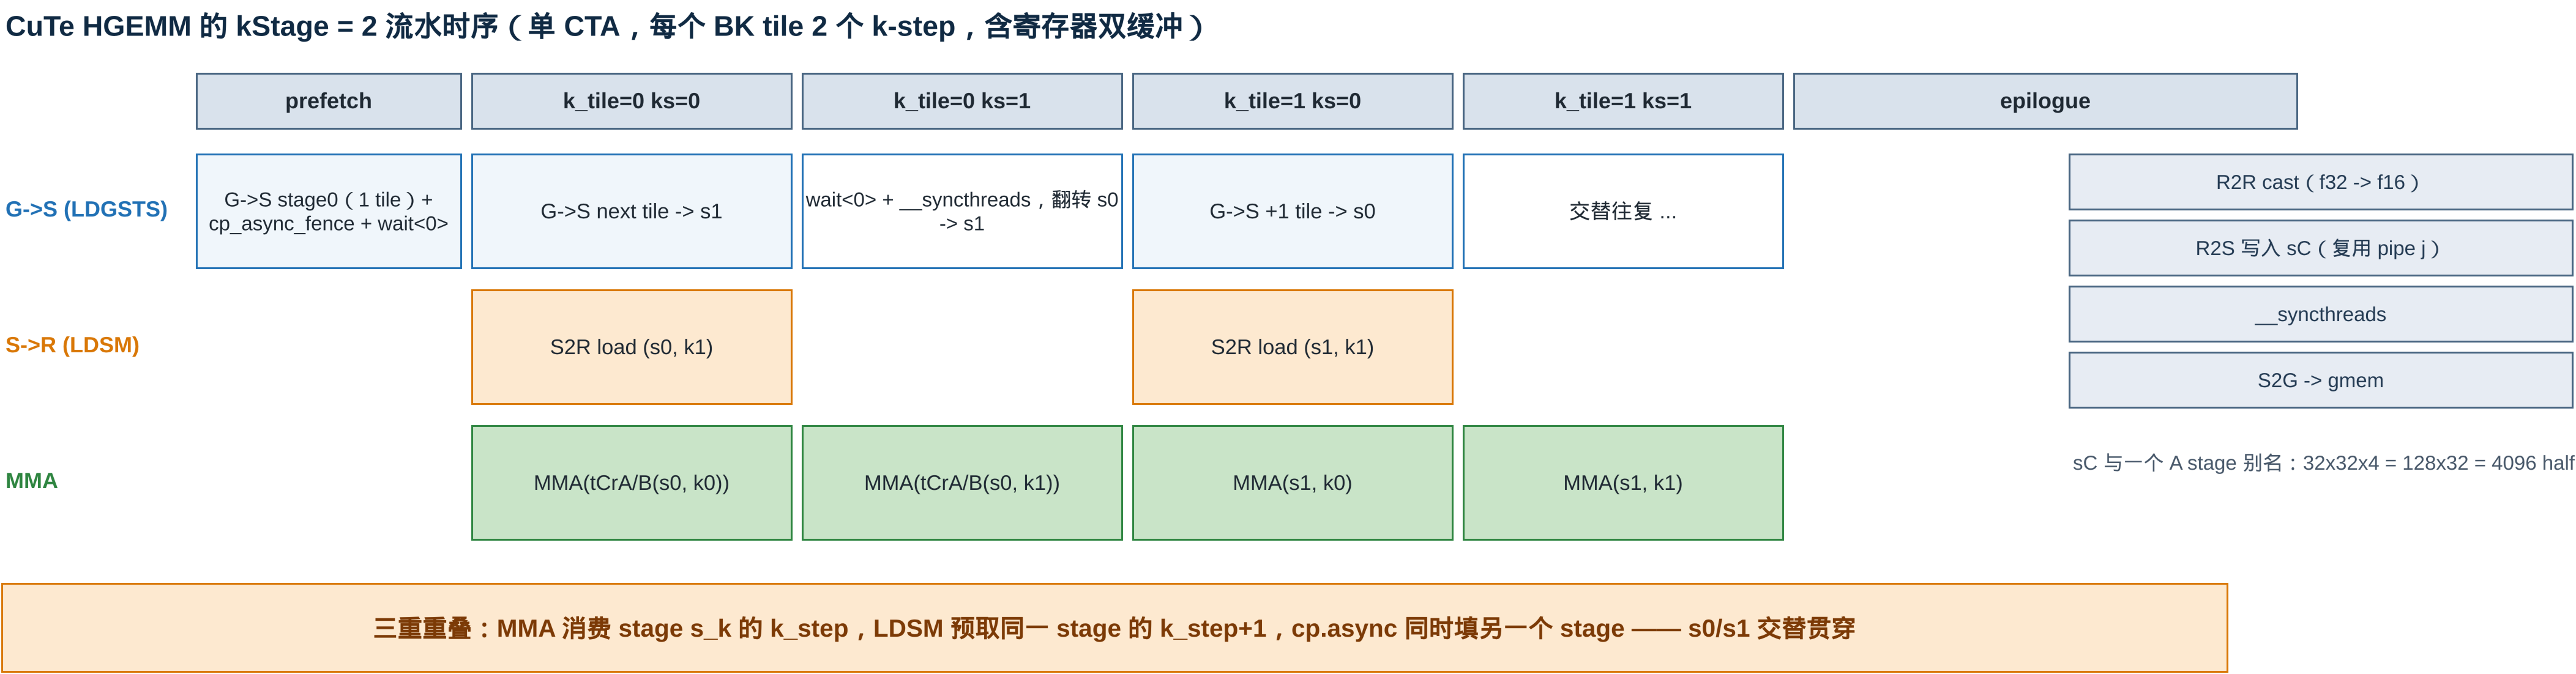
\includegraphics[width=0.95\textwidth]{figures/drawio/fig-24-2-kstage-pipeline/fig-24-2.png}
\begin{tikzpicture}[font=\tiny, >=Stealth,
  hdr/.style={draw=gray!55, fill=gray!14, align=center, inner sep=1.5pt,
    font=\fontsize{4}{4.5}\selectfont},
  cB/.style={draw=tkBlue, fill=tkFillBlue, align=center, inner sep=1.5pt,
    font=\fontsize{4}{4.5}\selectfont},
  cW/.style={draw=tkBlue!50, fill=white, align=center, inner sep=1.5pt,
    font=\fontsize{4}{4.5}\selectfont},
  cO/.style={draw=tkOrange, fill=tkFillOrange, align=center, inner sep=1.5pt,
    font=\fontsize{4}{4.5}\selectfont},
  cG/.style={draw=tkGreen, fill=tkFillGreen, align=center, inner sep=1.5pt,
    font=\fontsize{4}{4.5}\selectfont},
  cEpi/.style={draw=gray!60, fill=gray!12, align=center, inner sep=1.5pt,
    font=\fontsize{4}{4.5}\selectfont},
]
  % 时间列边界：0 / 1.75 / 4.10 / 6.45 / 8.80 / 11.15；epilogue 列 11.55-14.55
  \node[hdr, text width=1.60cm] at (0.875,0.87) {prefetch};
  \node[hdr, text width=2.20cm] at (2.925,0.87) {k\_tile$=$0\\ks$=$0};
  \node[hdr, text width=2.20cm] at (5.275,0.87) {k\_tile$=$0\\ks$=$1};
  \node[hdr, text width=2.20cm] at (7.625,0.87) {k\_tile$=$1\\ks$=$0};
  \node[hdr, text width=2.20cm] at (9.975,0.87) {k\_tile$=$1\\ks$=$1};
  \node[hdr, text width=2.85cm] at (13.05,0.87) {epilogue};
  % 泳道一：G->S（cp.async 填 smem）
  \node[cB, text width=1.60cm] at (0.875,-0.675)
    {G$\to$S s0\\（1 tile）\\$+$ fence\\$+$ wait$\langle0\rangle$};
  \node[cB, text width=2.20cm] at (2.925,-0.675) {G$\to$S 下一 tile $\to$ s1};
  \node[cW, text width=2.20cm] at (5.275,-0.675)
    {wait$\langle0\rangle$ $+$ \texttt{\_\_syncthreads}\\翻转 s0 $\to$ s1};
  \node[cB, text width=2.20cm] at (7.625,-0.675) {G$\to$S $+1$ tile $\to$ s0};
  \node[cB, text width=2.20cm] at (9.975,-0.675) {交替往复 $\cdots$};
  % 泳道二：S->R（ldmatrix 双缓冲）
  \node[cO, text width=2.20cm] at (2.925,-2.095) {S2R load (s0, k1)};
  \node[cO, text width=2.20cm] at (7.625,-2.095) {S2R load (s1, k1)};
  % 泳道三：MMA
  \node[cG, text width=2.20cm] at (2.925,-3.515) {MMA(tCrA/B(s0, k0))};
  \node[cG, text width=2.20cm] at (5.275,-3.515) {MMA(tCrA/B(s0, k1))};
  \node[cG, text width=2.20cm] at (7.625,-3.515) {MMA(s1, k0)};
  \node[cG, text width=2.20cm] at (9.975,-3.515) {MMA(s1, k1)};
  % 泳道标签
  \node[anchor=east, text=tkBlue, font=\bfseries\fontsize{4}{4.5}\selectfont]
    at (-0.15,-0.675) {G$\to$S (LDGSTS)};
  \node[anchor=east, text=tkOrange, font=\bfseries\fontsize{4}{4.5}\selectfont]
    at (-0.15,-2.095) {S$\to$R (LDSM)};
  \node[anchor=east, text=tkGreen, font=\bfseries\fontsize{4}{4.5}\selectfont]
    at (-0.15,-3.515) {MMA};
  % epilogue 四步（右列，不与三泳道同行）
  \node[cEpi, text width=2.85cm] at (13.05,-0.475) {R2R cast（f32 $\to$ f16）};
  \node[cEpi, text width=2.85cm] at (13.05,-1.575) {R2S 写入 sC（复用 pipe j）};
  \node[cEpi, text width=2.85cm] at (13.05,-2.675) {\texttt{\_\_syncthreads}};
  \node[cEpi, text width=2.85cm] at (13.05,-3.775) {S2G $\to$ gmem};
  \node[align=center, font=\fontsize{4}{4.5}\selectfont, text width=3.4cm]
    at (13.05,-4.56) {sC 与一个 A stage 别名：\\32$\times$32$\times$4 $=$ 128$\times$32 $=$ 4096 half};
  % 底部：三重重叠
  \node[draw=tkOrange, fill=tkFillOrange, text=tkOrange!80!black, align=center,
    font=\fontsize{4.2}{4.8}\selectfont, text width=15.2cm, inner sep=2pt]
    at (6.7,-5.18)
    {三重重叠：MMA 消费 stage $s_k$ 的 k\_step，LDSM 预取同一 stage 的 k\_step$+1$，%
     cp.async 同时填另一个 stage —— s0/s1 交替贯穿};
\end{tikzpicture}
\caption{CuTe HGEMM 的 $k_{\mathrm{stage}}=2$ 流水时序（含寄存器双缓冲）。上：G$\to$S（LDGSTS）；中：S$\to$R（LDSM）；下：MMA。MMA 消费 stage $s_k$ 的 k\_step 时，LDSM 预取同一 stage 的 k\_step+1，cp.async 同时填另一个 stage——三重重叠；左端 prefetch 一个 tile，右端 epilogue（R2R $\to$ R2S $\to$ S2G，sC 与一个 A stage 别名：$32{\times}32{\times}4 = 128{\times}32 = 4096$ half）。}
\label{fig:24-2}
\end{figure}

\begin{figure}[htbp]
\centering
% was: 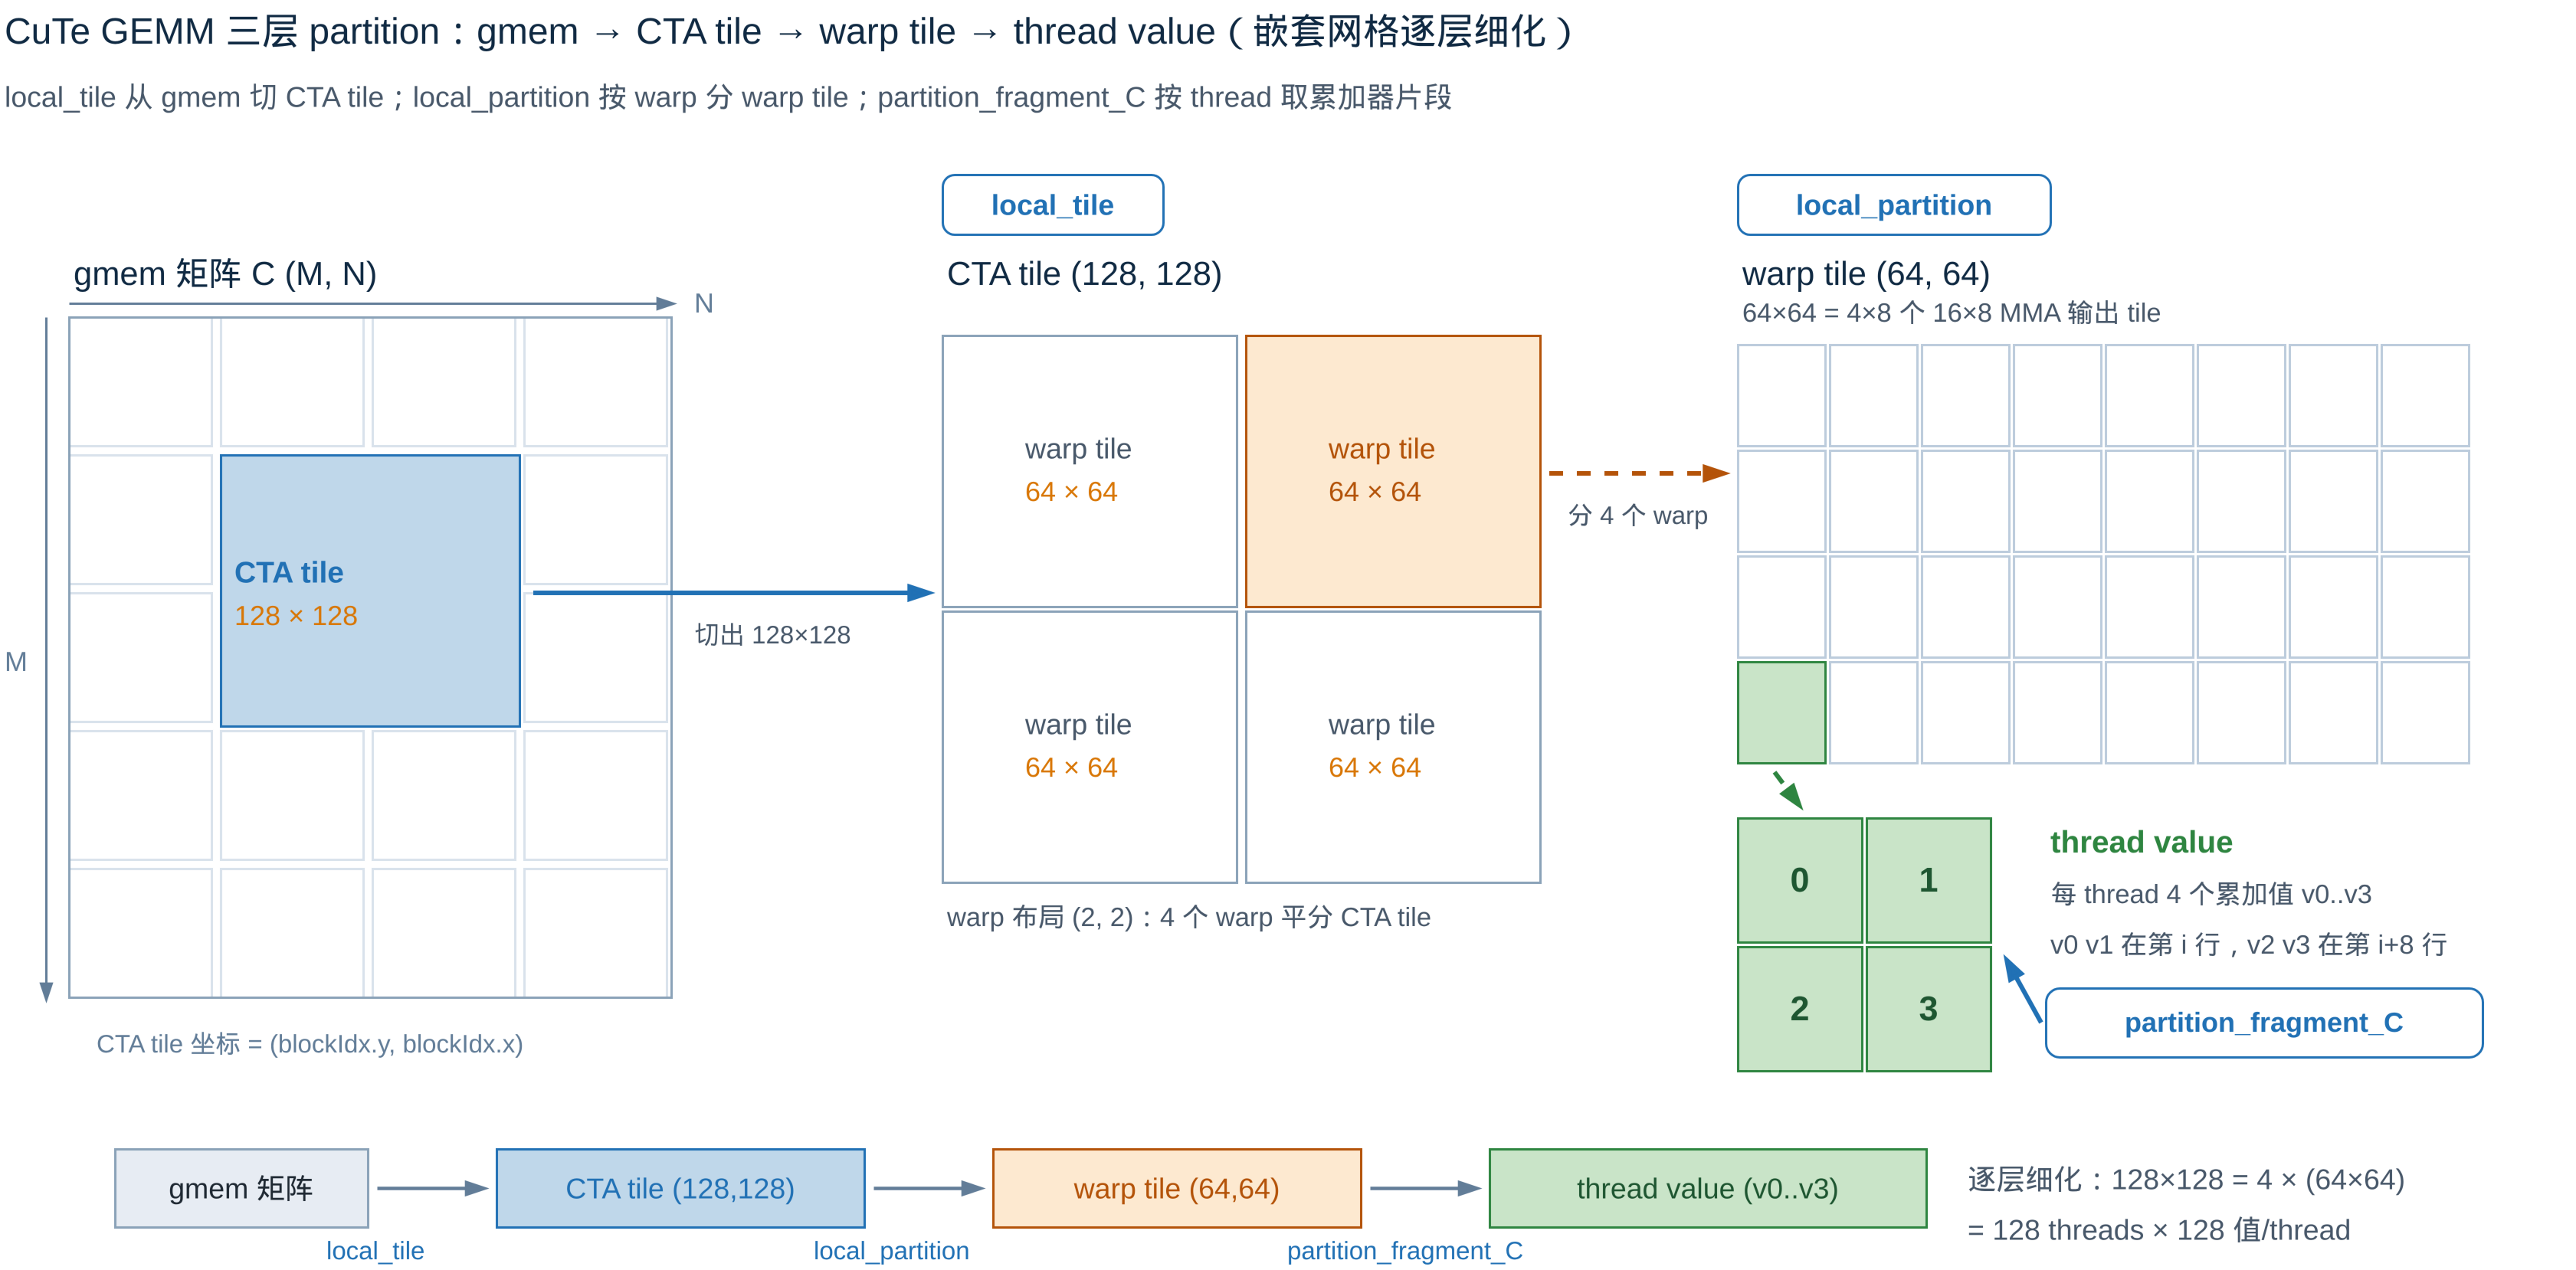
\includegraphics[width=0.95\textwidth]{figures/drawio/fig-24-3-gemm-3level-partition/fig-24-3.png}
\begin{tikzpicture}[font=\tiny, >=Stealth,
  pnl/.style={font=\fontsize{4.6}{5.2}\selectfont, inner sep=1pt},
  api/.style={draw=tkBlue, fill=tkFillBlue, rounded corners=1.5pt, text=tkBlue,
    align=center, inner sep=2pt, font=\fontsize{4}{4.5}\selectfont},
  small/.style={align=center, inner sep=1pt, font=\fontsize{4}{4.5}\selectfont},
]
  % 面板标题与 API 徽章（local_tile / local_partition 为所属层 API）
  \node[api] at (5.65,0.34) {local\_tile};
  \node[api] at (10.15,0.34) {local\_partition};
  \node[pnl, anchor=west] at (0.55,0.02) {gmem 矩阵 C (M, N)};
  \node[pnl, anchor=west] at (4.35,0.02) {CTA tile (128, 128)};
  \node[pnl, anchor=west] at (8.25,0.02) {warp tile (64, 64)};
  \node[small, anchor=west] at (8.25,-0.20) {64$\times$64 $=$ 4$\times$8 个 16$\times$8 MMA 输出 tile};
  % 面板 A：gmem 矩阵 4x5 格，CTA tile 覆盖中心 2x2 格
  \foreach \rr in {0,...,4} {
    \foreach \cc in {0,...,3} {
      \draw[gray!45, thin] ({0.55+0.60*\cc},{-0.45-0.54*\rr})
        rectangle ({0.55+0.60*\cc+0.60},{-0.45-0.54*\rr-0.54});
    }
  }
  \draw[gray!70, thick] (0.55,-0.45) rectangle (2.95,-3.15);
  \fill[tkFillBlue, draw=tkBlue, thick] (1.15,-0.99) rectangle (2.35,-2.07);
  \node[small] at (1.75,-1.37) {CTA tile};
  \node[small] at (1.75,-1.65) {128 $\times$ 128};
  \draw[->, gray!70, thin] (0.55,-0.30) -- (3.05,-0.30);
  \node[small, anchor=west] at (3.10,-0.30) {N};
  \draw[->, gray!70, thin] (0.32,-0.45) -- (0.32,-3.15);
  \node[small, anchor=center] at (0.16,-1.80) {M};
  \node[small, anchor=north, text width=2.60cm] at (2.00,-3.30)
    {CTA tile 坐标 $=$ (blockIdx.y, blockIdx.x)};
  % 面板 A -> B：local_tile 切出
  \draw[->, tkBlue, semithick] (3.05,-1.53) -- (4.35,-1.53);
  \node[small, text width=1.25cm] at (3.70,-1.72) {切出\\128$\times$128};
  % 面板 B：CTA tile = 2x2 warp tile（高亮右上角一个 warp）
  \foreach \rr in {0,...,1} {
    \foreach \cc in {0,...,1} {
      \pgfmathsetmacro{\xr}{4.35+1.30*\cc}
      \pgfmathsetmacro{\yr}{-0.45-1.12*\rr}
      \pgfmathtruncatemacro{\hi}{\cc - \rr}
      \ifnum\hi=1
        \fill[tkFillOrange] (\xr,\yr) rectangle (\xr+1.30,\yr-1.12);
        \draw[tkOrange, thick] (\xr,\yr) rectangle (\xr+1.30,\yr-1.12);
        \node[small, text=tkOrange!75!black] at (\xr+0.65,\yr-0.44) {warp tile};
        \node[small, text=tkOrange!75!black] at (\xr+0.65,\yr-0.70) {64 $\times$ 64};
      \else
        \draw[gray!60, thick] (\xr,\yr) rectangle (\xr+1.30,\yr-1.12);
        \node[small] at (\xr+0.65,\yr-0.44) {warp tile};
        \node[small] at (\xr+0.65,\yr-0.70) {64 $\times$ 64};
      \fi
    }
  }
  \node[small, anchor=north, text width=3.0cm] at (5.65,-2.78)
    {warp 布局 (2, 2)：4 个 warp 平分 CTA tile};
  % 面板 B -> C：local_partition 分给单个 warp
  \draw[->, dashed, tkOrange, semithick] (7.05,-1.10) -- (8.25,-1.10);
  \node[small, text width=1.2cm] at (7.65,-1.30) {分 4 个\\warp};
  % 面板 C：warp tile = 4x8 个 16x8 MMA 输出格；左下格放大为 thread 累加片段
  \foreach \rr in {0,...,3} {
    \foreach \cc in {0,...,7} {
      \draw[gray!45, thin] ({8.25+0.40*\cc},{-0.45-0.36*\rr})
        rectangle ({8.25+0.40*\cc+0.40},{-0.45-0.36*\rr-0.36});
    }
  }
  \fill[tkFillGreen, draw=tkGreen, thick] (8.25,-1.89) rectangle (8.65,-1.53);
  \draw[gray!70, thick] (8.25,-0.45) rectangle (11.45,-1.89);
  \draw[->, dashed, tkGreen, semithick] (8.45,-1.96) -- (8.62,-2.30);
  \foreach \rr in {0,...,1} {
    \foreach \cc in {0,...,1} {
      \pgfmathsetmacro{\xb}{8.25+0.55*\cc}
      \pgfmathsetmacro{\yb}{-2.35-0.55*\rr}
      \pgfmathtruncatemacro{\vi}{2*\rr+\cc}
      \fill[tkFillGreen, draw=tkGreen, thick] (\xb,\yb) rectangle (\xb+0.50,\yb-0.50);
      \node[font=\fontsize{4.6}{5.2}\selectfont, text=tkGreen!75!black]
        at (\xb+0.25,\yb-0.25) {v\vi};
    }
  }
  \node[font=\bfseries\fontsize{4}{4.5}\selectfont, text=tkGreen, anchor=west]
    at (9.40,-2.52) {thread value};
  \node[small, anchor=west] at (9.40,-2.76) {每 thread 4 个累加值 v0..v3};
  \node[small, anchor=west] at (9.40,-3.00) {v0 v1 在第 $i$ 行，v2 v3 在第 $i{+}8$ 行};
  \node[api, text width=1.95cm] at (10.50,-3.62) {partition\_fragment\_C};
  \draw[->, tkBlue, semithick] (9.46,-3.55) -- (9.30,-3.42);
  % 底部层级链：四层对象 + 三个 API
  \node[draw=gray!65, fill=gray!12, align=center, inner sep=2pt,
    font=\fontsize{4.2}{4.8}\selectfont, text width=1.50cm] at (1.65,-4.58) {gmem 矩阵};
  \node[draw=tkBlue, fill=tkFillBlue, text=tkBlue, align=center, inner sep=2pt,
    font=\fontsize{4.2}{4.8}\selectfont, text width=2.20cm] at (4.70,-4.58) {CTA tile (128,128)};
  \node[draw=tkOrange, fill=tkFillOrange, text=tkOrange!80!black, align=center,
    inner sep=2pt, font=\fontsize{4.2}{4.8}\selectfont, text width=2.20cm]
    at (8.10,-4.58) {warp tile (64,64)};
  \node[draw=tkGreen, fill=tkFillGreen, text=tkGreen!80!black, align=center,
    inner sep=2pt, font=\fontsize{4.2}{4.8}\selectfont, text width=2.60cm]
    at (11.70,-4.58) {thread value (v0..v3)};
  \draw[->, gray!70, semithick] (2.44,-4.58) -- (3.56,-4.58);
  \draw[->, gray!70, semithick] (5.84,-4.58) -- (6.96,-4.58);
  \draw[->, gray!70, semithick] (9.24,-4.58) -- (10.36,-4.58);
  \node[small, text=tkBlue] at (3.00,-4.86) {local\_tile};
  \node[small, text=tkBlue] at (6.40,-4.86) {local\_partition};
  \node[small, text=tkBlue] at (9.80,-4.86) {partition\_fragment\_C};
  \node[small, anchor=west, text width=2.00cm] at (13.15,-4.45)
    {逐层细化：\\128$\times$128 $=$ 4 $\times$ (64$\times$64)\\
     $=$ 128 threads $\times$ 128 值/thread};
\end{tikzpicture}
\caption{CuTe GEMM 的三层 partition：\texttt{local\_tile} 以 \texttt{\allowbreak{}(block\allowbreak{}Idx.\allowbreak{}y,\allowbreak{} block\allowbreak{}Idx.\allowbreak{}x)} 为坐标从 gmem 切出 CTA tile $(128,128)$；warp 布局 $(2,2)$ 下 \texttt{local\_\allowbreak{}partition} 平分给 4 个 warp 得 $(64,64)$；warp tile 由 $4\times8$ 个 $16\times8$ atom 铺满，\texttt{partition\_\allowbreak{}fragment\_\allowbreak{}C} 为每 thread 生成累加器片段（单 MMA tile 内 $2\times2$ 四值，v0/v1 在第 $i$ 行、v2/v3 在第 $i+8$ 行）。层级换算 $128\times128=4\times(64\times64)=128$\,threads$\times128$ 值/thread。重建自 @reed《cute 之 简单 GEMM 实现》（示意图为经典 4-warp/$64\times64$ 配置；本章 kernel 实为 tile $32\times32$、warp $16\times16$，层级方法相同）。}
\label{fig:24-3}
\end{figure}

\section{性能分析}

本章没有为 CuTe HGEMM 单独建 bench（Phase~7c 的集成数据由 \texttt{bench/bench\_leetcuda.cu}
的 \texttt{--bench} 统一采集）。这里只给三条可核验的定量结论：

\begin{enumerate}
  \item \textbf{正确性}：最小测试在 $128\times256\times64$（F16 累加）与
        $128\times128\times64$（F32 累加）两组形状上分别以
        \texttt{TOL\_F16ACC}$=5\times10^{-2}$、\texttt{TOL\_F32ACC}$=10^{-3}$
        判定通过（第~\ref{sec:24-minitest}~节给出实测 \texttt{max\_abs\_err}）。
  \item \textbf{寄存器压力}：\texttt{ptxas -v} 实测两种配置的寄存器数与 stack
        使用（实测值见本节的实践须知），核对源码注释里\textbf{均 0 spill}的说法。
  \item \textbf{smem 占用}：式~\eqref{eq:24-smem} 的 48\,KiB 由
        \texttt{cosize\allowbreak{}(Smem\allowbreak{}Layout\allowbreak{}A) + cosize\allowbreak{}(Smem\allowbreak{}Layout\allowbreak{}B)} 在
        编译期算出。同一个常量既决定 \texttt{cuda\allowbreak{}Func\allowbreak{}Set\allowbreak{}Attribute} 的实参，也决定
        occupancy 上限。$B_N$ 降到 128（F32 累加）时它同步降到 32\,KiB，
        精度换占用的取舍是类型参数的直接后果。
\end{enumerate}

\paragraph{实践须知：两处源码注释的性能口径}\label{sec:24-kaogu}

\begin{itemize}
  \item \textbf{$B_N$ 随累加精度切换的寄存器断言}（hgemm.cuh L1229--1230）：
        注释称\textbf{F16 acc 用 256（$128\times256$ tile，0 spill）；F32 acc 用 128
        （$128\times128$ tile，0 spill）。F32 $+$ $B_N{=}256$ 会产生
        $\sim$1\,KB spill（254 reg），性能下降 3--8 倍}。用
        \texttt{nvcc -Xptxas -v} 编译本 wrapper 的两种实例化（与本章测试同源）
        实测：$B_N{=}256$/F16 用 254 个寄存器、$B_N{=}128$/F32 用 226 个，
        \textbf{两者 stack frame 均为 0 字节}（0 spill stores / 0 spill loads），
        与注释前两句一致。
  \item 注释第三句描述的组合在本 wrapper 里\textbf{不可达}：\texttt{kBN} 由
        \texttt{kAccF32} 单向决定，F32 累加永远配不到 $B_N=256$，属于手工改坏
        才会遇到的反例。测量值本身有效（它是 $B_N{=}256$ 那一档的
        254\,reg），只是不该被读成\textbf{本 kernel 的第三种配置}；复现方法见
        第~\ref{sec:24-minitest}~节动手实验第 3 条。
  \item \textbf{代码量对照}（hgemm.cuh L803--805）：注释写\textbf{手写 $\sim$200 行 /
        CuTe $\sim$80 行}。按同口径实测（去注释、去空行）：手写 Phase~7b 为
        151 行、Phase~7b-3 为 235 行，CuTe kernel 本体为 118 行（另有 launch
        wrapper 86 行）。注释给的是量级估计，方向正确（CuTe 版确实更短），但
        \textbf{$\sim$80 行}低估了约三成；本章一律以实测数字为准
        （图~\ref{fig:24-1}）。
\end{itemize}

\paragraph{实测性能：CuTe Swizzle 家族 vs cuBLAS}\label{sec:ch24-perf}

前面几条验证的都是本章自己给的数字，再给一组对外的对照：第~\ref{ch:20}--\ref{ch:23}~章
铺垫的 layout 代数、\texttt{TiledCopy}、\texttt{TiledMMA}、swizzle 组合子落到
真实负载上究竟值多少？用 \texttt{leetcuda\_\allowbreak{}bench\_\allowbreak{}sm120a.\allowbreak{}bin} 的
\texttt{--bench --bench-all} 在 RTX PRO 5000（sm\_120，110 SM，CUDA 13.2）上实测
$M{=}N{=}K{=}8192$ 的 fp16 HGEMM，CuTe Swizzle 家族七个配置见
表~\ref{tab:ch24-perf}：F16Acc 档追平乃至超越 cuBLAS f16（分母为同轮 cuBLAS
f16 的 246.5\,TFLOPS，本家族 0.99$\sim$1.08$\times$，最高 1.08$\times$），F32Acc 档
对比 cuBLAS f32（164.2\,TFLOPS）达 1.48$\times$。七个配置的 Max Err 全部为
$0.000\mathrm{e}{+}00$，逐位零误差。这些地址算术在编译期被类型系统全部折叠成
最终指令，实测说明这套抽象是零开销的。

\begin{table}[H]
\centering
\caption{HGEMM CuTe Swizzle 实测（RTX PRO 5000，M=N=K=8192，fp16）}
\label{tab:ch24-perf}
\footnotesize
\setlength{\tabcolsep}{4pt}
\begin{tabular}{lrr}
\toprule
Kernel & Max Err & TFLOPS/cuBLAS（加速比） \\
\midrule
HGEMM CuTe Swizzle (S=2, BLK\_SW=0, F16Acc) & 0.000e+00 & 243.0/246.5 (0.99x) \\
HGEMM CuTe Swizzle (S=2, BLK\_SW=0, F32Acc) & 0.000e+00 & 201.3/164.2 (1.23x) \\
HGEMM CuTe Swizzle (S=2, BLK\_SW=1, F16Acc) & 0.000e+00 & 250.2/246.5 (1.01x) \\
HGEMM CuTe Swizzle (S=2, BLK\_SW=1, F32Acc) & 0.000e+00 & 226.0/164.2 (1.38x) \\
HGEMM CuTe Swizzle (S=3, BLK\_SW=0, F16Acc) & 0.000e+00 & 257.2/246.5 (1.04x) \\
HGEMM CuTe Swizzle (S=3, BLK\_SW=1, F16Acc) & 0.000e+00 & 265.9/246.5 (1.08x) \\
HGEMM CuTe Swizzle (S=3, BLK\_SW=1, F32Acc) & 0.000e+00 & 242.4/164.2 (1.48x) \\
\bottomrule
\end{tabular}
\end{table}

CuTe 版\textbf{不承诺}比手写版更快。两者的指令序列高度重合
（SASS 层面都是 \texttt{LDGSTS} $+$ \texttt{LDSM} $+$ \texttt{HMMA}），差别在
编译期把地址算术折叠掉、以及让 kernel 作者少写上百行易错的表达式。真正的加速
来自第~\ref{ch:12}~章那样的算法级决策（swizzle 档位、block swizzle、
寄存器双缓冲）；CuTe 的价值是让这些决策更容易表达、检查与复用。

\section{常见坑}

\begin{enumerate}
  \item B 必须转置传入。式~\eqref{eq:24-tn} 的 TN 语义要求 \texttt{Bptr} 指向
        $B^{\mathsf T}[N,K]$ 的 row-major 存储。直接把 row-major 的 $B[K,N]$
        传进去不会报错，只会算错。最小测试在 host 侧显式构造转置。
  \item 没有 tile 内 predication。kernel 只有 CTA 级边界判断，调用方必须保证
        $M \% B_M = 0$、$N \% B_N = 0$、$K \% B_K = 0$；这也决定了本章测试
        形状取 $128/256/64$（$M=N=K=64$ 用不了：$B_M=128$）。
  \item $B_N$ 与累加精度绑定。\texttt{k\allowbreak{}Acc\allowbreak{}F32=\allowbreak{}true} 时 $B_N$ 自动降到 128；
        手工把 F32 累加配到 $B_N=256$（本 wrapper 不可达的组合）会让累加器
        超出可用寄存器、溢出到 local memory（第~\ref{sec:24-kaogu}~节）。
  \item 动态 smem 必须显式提额。\texttt{cuda\allowbreak{}Func\allowbreak{}Set\allowbreak{}Attribute} 在 wrapper 里、
        launch 之前；漏掉它只会在 $k_{\mathrm{stage}}$ 较大时启动失败。
  \item BlockSwizzle 改变 grid 维度。开关打开后 grid 是 3D 且 \texttt{BX} 要按
        \texttt{BZ} 折算；只改 kernel 模板参数而不改 host 侧 grid 会索引错 block。
  \item epilogue 别漏 \texttt{\_\allowbreak{}\_\allowbreak{}syncthreads\allowbreak{}()}。R2S 与 S2G 之间必须汇合：
        S2G 读的是其它线程刚写入 sC 的数据；漏掉会得到大部分正确、偶发错误的
        结果。
  \item $k_{\mathrm{stage}}$ 与 smem 的联动。$k_{\mathrm{stage}}$ 从 2 加到 3 会把
        式~\eqref{eq:24-smem} 的 A$+$B 部分抬高 50\%；\texttt{kShmSize} 与
        \texttt{cuda\allowbreak{}Func\allowbreak{}Set\allowbreak{}Attribute} 会自动跟着变，但 occupancy 会下降，
        这是改一个模板参数的连带代价。
\end{enumerate}

\section{面试要点速查}

\begin{enumerate}
  \item \textbf{Q}：CuTe 版 HGEMM 比手写版短在哪？
        \textbf{A}：短在地址算术：smem 寻址、swizzle、\texttt{ldmatrix} lane 映射、
        epilogue shuffle 四类表达式全部由类型推导取代；流水线的
        同步逻辑（fence/wait/计数器）两边一样要手写。
  \item \textbf{Q}：\texttt{cute::gemm} 自动展开了哪些循环？
        \textbf{A}：对 $(V,M,K)\times(V,N,K)$ 输入，
        \texttt{MMA\_M}$\times$\texttt{MMA\_N}$\times$\texttt{MMA\_K}
        都会被展开。外层 K-tile 的搬运循环仍需手写；本章显式
        \texttt{k\_step} 则服务于寄存器双缓冲，不是 \texttt{gemm} 的能力限制。
  \item \textbf{Q}：为什么 $B_K=32$ 而不是 64？
        \textbf{A}：smem 预算与切片粒度的折中：$B_K=32$ 时
        $n_{k\text{-step}}=2$、A$+$B 双 stage 占 48\,KiB；$B_K$ 翻倍会同步
        抬高 smem 并挤压 occupancy。
  \item \textbf{Q}：\texttt{make\_\allowbreak{}tiled\_\allowbreak{}copy\_\allowbreak{}A} 为什么不需要指定
        ThrLayout？
        \textbf{A}：它从 \texttt{tiled\_mma} 反推：S$\to$R 的线程映射必须与
        MMA fragment 的分布共形，两者是同一事实的两种表述。
  \item \textbf{Q}：epilogue 为什么经 smem 中转？
        \textbf{A}：累加器 fragment 的寄存器分布不适合直接宽写 gmem；经 smem
        做一次 CTA 范围的数据重组（R2S $+$ S2G），才能用 128-bit 宽写，
        并且避免手写跨 lane 的 shuffle 编排。
  \item \textbf{Q}：换成 F32 累加要动哪些地方？
        \textbf{A}：换 atom（\texttt{SM80\_\allowbreak{}16x8x16\_\allowbreak{}F32\allowbreak{}F16\allowbreak{}F16\allowbreak{}F32\_\allowbreak{}TN}），
        $B_N$ 随之降到 128，其余（C scratchpad pipe、R2S cast、S2G 宽写）
        由同一套类型推导覆盖，这是类型即配置的收益。
\end{enumerate}

\section{最小测试与动手实验}\label{sec:24-minitest}

\texttt{book/\allowbreak{}tests/\allowbreak{}ch24\_\allowbreak{}hgemm\_\allowbreak{}cute.cu} 的逻辑照抄 \texttt{bench/hgemm.cu}
L192 的 \texttt{test\_\allowbreak{}hgemm\_\allowbreak{}cute}，但按本书测试规范改造：参考值换成
\textbf{CPU fp64 三重循环}（不依赖 cuBLAS），判定走 \texttt{book\_check}
容差三档。测试跑两组配置：

\begin{itemize}
  \item 第一组：\texttt{launch\_\allowbreak{}hgemm\_\allowbreak{}mma\_\allowbreak{}stages\_\allowbreak{}tn\_\allowbreak{}cute\allowbreak{}<half, 2, 0, false>}，
        $M{=}128,N{=}256,K{=}64$，容差 \texttt{TOL\_F16ACC}$=5\times10^{-2}$；
  \item 第二组：\texttt{launch\_\allowbreak{}hgemm\_\allowbreak{}mma\_\allowbreak{}stages\_\allowbreak{}tn\_\allowbreak{}cute\allowbreak{}<half, 2, 0, true>}，
        $M{=}128,N{=}128,K{=}64$，容差 \texttt{TOL\_F32ACC}$=10^{-3}$。
\end{itemize}

规模约束来自 kernel 的整除要求（$M\%128=0$、$N\%B_N=0$、$K\%32=0$），同时满足
BOOK\_PLAN §6\textbf{CPU 参考规模 $\le 512$}的时限约束。编译与运行：

\begin{lstlisting}[style=console]
cd kernels/interview/book/tests
CUDA_VISIBLE_DEVICES=6 ./build_tests.sh --arch sm_120a --ch ch24
\end{lstlisting}

本机运行输出（RTX PRO 5000，CUDA 13.2，CUTLASS v4.6.1，2026-09-11）：

\begin{lstlisting}[style=console]
== ch24_hgemm_cute.cu (sm_120a)
PASS HGEMM CuTe F16Acc 128x256x64: max_abs_err=4.376e-04 (tol=5.0e-02)
PASS HGEMM CuTe F32Acc 128x128x64: max_abs_err=2.897e-04 (tol=1.0e-03)
ALL OK
\end{lstlisting}

两组输入的随机数幅度缩到 $\pm0.25$：fp16\textbf{输出}的舍入误差量级是
$|C|\cdot2^{-11}$，只有把 $|C|$ 压在 $2$ 附近，$10^{-3}$ 这条容差才是在
检验\textbf{累加精度}而不是\textbf{输出量化}。带上 \texttt{bench} 参数还能跑一版
吞吐计时（$K{=}64$ 的规模只有微秒级，被 launch 开销主导，不构成性能结论；
端到端吞吐对照见第~\ref{sec:ch24-perf}~节）。

代码量的统计口径（图~\ref{fig:24-1} 的数字）只统计非空、非纯注释行，
用一条 \texttt{awk} 命令即可复现。动手实验建议三条：

\begin{enumerate}
  \item 把 \texttt{Stages} 从 2 改成 3，观察 smem 涨到 72\,KiB 量级、
        \texttt{cuda\allowbreak{}Func\allowbreak{}Set\allowbreak{}Attribute} 的实参随之变化。
  \item 把 \texttt{Block\allowbreak{}Swizzle} 置 1 并改 host 侧 grid 为 3D，用同一组形状
        验证结果不变（只影响 L2 局部性，不影响正确性）。
  \item 把 \texttt{kAccF32} 置 true 但手工把 \texttt{kBN} 改回 256，用
        \texttt{-Xptxas -v} 看 spill 报告，复现第~\ref{sec:24-kaogu}~节提到的反例。
\end{enumerate}

\section*{延伸阅读}

\begin{itemize}
  \item @reed《cute 之 简单 GEMM 实现》，
        \url{https://zhuanlan.zhihu.com/p/667521327}
        （从零搭 CuTe GEMM 的三步骨架，本章第~\ref{sec:24-step1}~节按它展开）。
  \item @reed《cute 之 GEMM 流水线》，
        \url{https://zhuanlan.zhihu.com/p/665082713}
        （multistage 流水的 CuTe 写法与\textbf{流水线不属于 cute}的结论，本章
        第~\ref{sec:24-step2}~节按它展开）。
  \item @reed《cute 之 高效 GEMM 实现》，
        \url{https://zhuanlan.zhihu.com/p/675308830}
        （访存/计算/尾阶段高效与主机端类型清单，对应本章
        第~\ref{sec:24-step3a}、\ref{sec:24-step3b}~节）。
  \item @竹熙佳处《写给大家看的 CuTe 教程：async pipeline》，
        \url{https://zhuanlan.zhihu.com/p/2024832248386528275}
        （可对照本章\textbf{流水线仍要手写}的结论）；
  \item @进击的Killua《CUTLASS CuTe 实战（一）：基础》，
        \url{https://zhuanlan.zhihu.com/p/690703999}
        （Tensor 常用 API 速查，适合边看本章代码边查手册）。
\end{itemize}

% ch25-cute-flash-attn.tex — CuTe 应用（二）：FlashAttention 三实现对照（agent-ch25 撰写，2026-09-11）
% 源码区间（anchors.yaml ch25）：flash_attn.cuh L2196-3488（NOTES_V2_ENABLE_CUTE 宏块）
% \url 由 book.tex 的 hyperref 提供；单章独立编译时降级为可断行的 \ttfamily
\makeatletter
\providecommand{\urlchbrk}[1]{\@tfor\next:=#1\do{\next\allowbreak}}
\makeatother
\providecommand{\url}[1]{{\ttfamily\urlchbrk{#1}}}
\chapter{CuTe 应用（二）：FlashAttention 三实现对照}\label{ch:25}

\section{本章导读}

第~\ref{ch:16}--\ref{ch:18}~章我们用手写地址算术实现了三代 FlashAttention：
FA2 的 Split-Q + cp.async 多级流水（flash\_attn.cuh L5--790）、FA2 的 TMA + warp
specialization（L792--1440）、FA3 的双 consumer warpgroup（L1441--2192）。三代实现
都在做同一件事：把 $S=QK^\top$、online softmax、$O=PV$ 三段落进张量核与搬运
流水之间；但每一代都要重写一遍 Q/K/V 的 smem 布局、fragment 的 lane 映射、
ldmatrix 的地址算术与屏障协议。这不是作者偷懒：布局事实在 C++/PTX 里没有
独立的落脚点，swizzle 常量、lane 位段、寄存器编号只能以裸算术的形式与计算
逻辑混写在一起。

本章问一个具体的问题：把这些布局事实搬进类型之后，同一段 attention 会长什么
样？答案是同一文件第四个区段的四个 CuTe 实现（L2196--3488，
\texttt{NOTES\_\allowbreak{}V2\_\allowbreak{}ENABLE\_\allowbreak{}CUTE} 宏块）。它们不是四份互不相干的代码，而是
同一个算法的三级搭建：实现 1
\texttt{flash\_\allowbreak{}attn\_\allowbreak{}mma\_\allowbreak{}stages\_\allowbreak{}split\_\allowbreak{}q\_\allowbreak{}cute}（cp.async + 统一流水，256 线程）最朴素，
组装方式照 @reed《cute 之 简单 GEMM 实现》的 Tensor $\to$ \texttt{local\_tile}
$\to$ partition $\to$ copy/gemm 四步走：数据怎么切、怎么分给线程、怎么搬、
怎么算，一一对应到 CuTe 抽象；实现 2
\texttt{flash\_\allowbreak{}attn\_\allowbreak{}tma\_\allowbreak{}mma\_\allowbreak{}ws\_\allowbreak{}split\_\allowbreak{}q\_\allowbreak{}cute}（TMA + producer/consumer 分工，
384 线程）在同一个算法上把搬运与计算解耦；实现 3
\texttt{flash\_\allowbreak{}attn\_\allowbreak{}3\_\allowbreak{}tma\_\allowbreak{}mma\_\allowbreak{}ws\_\allowbreak{}split\_\allowbreak{}q\_\allowbreak{}cute} 进一步采用 FA3 式双 consumer
（奇偶拆 KV + 终态归并）。第四个实现
\texttt{flash\_\allowbreak{}attn\_\allowbreak{}3\_\allowbreak{}cute\_\allowbreak{}tma\_\allowbreak{}copy\_\allowbreak{}smoke}（42 行）不是 attention，而是
一条 TMA 搬运链路的自检闭环，用来先把搬运与计算解耦，再单独排查。这是
Part~IV 的倒数第二章，也是抽象换代码量这条主线在 attention 上的完整样本。

本章的组织以动机为线：三级搭建逐级回答上一级留下的问题：实现 1
的浪费在哪、为什么实现 2 要把搬运拆出去、为什么实现 3 要拆 KV。四个实现共享
同一组编译期布局类型（\texttt{Flash\allowbreak{}Attn2\allowbreak{}Cu\allowbreak{}Te\allowbreak{}Traits} /
\texttt{Flash\allowbreak{}Attn3\allowbreak{}Cu\allowbreak{}Te\allowbreak{}Traits}）与五个 kernel 级工具函数，
这是第~\ref{ch:22}~章 TiledMMA 与 fragment 在真实 kernel 里的落点：

\begin{itemize}[itemsep=1pt,topsep=2pt]
  \item \texttt{convert\_\allowbreak{}layout\_\allowbreak{}acc\_\allowbreak{}rowcol} 与 \texttt{convert\_\allowbreak{}layout\_\allowbreak{}acc\_\allowbreak{}Aregs}
        是两个 fragment 重排函数（25.3.3/25.3.4 节）；
  \item \texttt{convert\_\allowbreak{}type}、\texttt{gemm\_ss}、\texttt{gemm\_rs} 负责类型转换与
        两个 GEMM 调用范式（25.4.1 节）。
\end{itemize}

五个函数里，\texttt{convert\_\allowbreak{}layout\_\allowbreak{}acc\_\allowbreak{}Aregs} 单独成节：$P$
（softmax 后的分数矩阵）要从 QK 的累加器变成 PV 的左操作数，@竹熙佳处
《写给大家看的 CuTe 教程：Layout Compose \& Inverse》讨论的正是这个场景。

\textbf{前置章节}：第~\ref{ch:17}~章（手写 TMA+WS 的 mbarrier 协议）、
第~\ref{ch:18}~章（FA3 双 consumer 与 merge）、第~\ref{ch:21}~章
（Tensor 与 TiledCopy：G2S/S2R 分工）、第~\ref{ch:22}~章（TiledMMA、EURepeat、
fragment 与 rowcol 变换）。\textbf{源码区间}：flash\_attn.cuh L2196--3488。
\textbf{编译宏}：\texttt{NOTES\_\allowbreak{}V2\_\allowbreak{}ENABLE\_\allowbreak{}CUTE}（四个实现都需要 TMA 或
cp.async 的 CuTe 抽象；sm80+ 可编）；后三个实现另需
\texttt{NOTES\_\allowbreak{}V2\_\allowbreak{}ENABLE\_\allowbreak{}TMA\_\allowbreak{}MMA\_\allowbreak{}WS}（TMA 指令，sm90+ 硬件）。
本节默认实例化取 $D\in\{64,128\}$、$B_r\in\{64,128\}$、$B_c=64$。
配套最小测试 \texttt{book/\allowbreak{}tests/\allowbreak{}ch25\_\allowbreak{}fa\_\allowbreak{}cute.\allowbreak{}cu}（三种形状的端到端正确性）。

\section{问题与动机}

先摊开手写版的维护面。第~\ref{ch:16}~章的 FA2 kernel 共 564 行有效代码，其中与
布局事实直接相关的至少有五类，且每一类都以裸地址算术的形式出现：

\begin{enumerate}
  \item \textbf{smem 行距与 padding}：$kSmemStrideQ/K/V = D+\mathrm{pad}$，
        pad 取 8 个 half 使 ldmatrix 的 8 行起始 bank 铺满 32 个 bank；
        $pk$ 与 $kPad$ 的组合还决定走 XOR swizzle 还是 padding 路径；
  \item \textbf{ldmatrix 的 lane 映射}：Q 用 \texttt{ldmatrix.x4}、
        K 用 \texttt{ldmatrix.x2}、V 用 \texttt{ldmatrix.\allowbreak{}x2.trans}，
        三者的行/列由 \texttt{lane} 的位段手工拼出；
  \item \textbf{fragment 的寄存器编号}：$R\_S[8][2]$、$R\_O/R\_D[8][2]$
        是哪个寄存器对应矩阵哪个元素的硬编码答案，4-lane 归约宽度
        （\texttt{warp\_\allowbreak{}reduce\allowbreak{}<4>}）也是从这套编号推出来的；
  \item \textbf{搬运粒度的地址划分}：256 线程协作加载时
        \texttt{load\_\allowbreak{}smem\_\allowbreak{}Q\_\allowbreak{}Br =\allowbreak{} tid/\allowbreak{}2} 这类映射；
  \item \textbf{屏障计数}：producer/consumer 的 arrive\_count（第~\ref{ch:17}~章
        的 257 协议、第~\ref{ch:18}~章的 per-WG 129）。
\end{enumerate}

第~\ref{ch:20}~章已经论证过这五类事实的联动代价：改一个 tile 尺寸，至少三处
要跟着改，且错误是静默的。CuTe 版的答案是把它们全部收进
\textbf{编译期类型}：smem 布局是 \texttt{tile\_\allowbreak{}to\_\allowbreak{}shape} 的返回类型、fragment
布局是 \texttt{partition\_\allowbreak{}fragment\_\allowbreak{}A/B/C} 的返回类型、搬运是
\texttt{TiledCopy} 的 TV 划分、连 V 的转置视图都是
\texttt{composition} 表达式的类型。kernel 正文里只剩三类语句：
数据流（\texttt{copy}/\texttt{gemm}）、同步（barrier / \texttt{cp.\allowbreak{}async.\allowbreak{}wait}）
与 online softmax 的标量运算。抽象掉了什么，可以逐项核对：\textbf{坐标计算}
收进 \texttt{local\_tile}/\texttt{partition} 的类型、\textbf{fragment 手工索引}
收进 \texttt{partition\_\allowbreak{}fragment} 的返回布局、\textbf{拷贝指令的选择}
收进 \texttt{TiledCopy} 的原子类型（G2S 选 cp.async 还是 TMA、S2R 选哪个
ldmatrix 形态）；三件事都不再出现在 kernel 正文里。

量化一下收益。表~\ref{tab:25-code} 用区间总行数除以去注释空行的有效代码行数，
对照三对实现（手写版区间与 CuTe 版区间都取自同一文件，统计口径一致：行以
\texttt{\textbackslash n} 计，注释行指以 \texttt{//} 开头的行）。

\begin{table}[htbp]
\centering
\caption{手写版与 CuTe 版的有效代码行数对照（flash\_attn.cuh，2026-09-11 统计）。
「结构件」指 FA2/FA3 traits 与五个工具函数，它们被后四个实现共享。}
\label{tab:25-code}
\begin{tabular}{llrr}
\toprule
实现 & 区间 & 总行数 & 有效代码行 \\
\midrule
FA2 手写（Split-Q + cp.async） & L5--790 & 786 & 564 \\
FA2 手写（TMA + WS） & L792--1440 & 649 & 451 \\
FA3 手写（双 consumer） & L1441--2192 & 752 & 515 \\
\midrule
CuTe 结构件（traits + 5 个工具函数） & L2197--2490 & 294 & 107 \\
CuTe 实现 1（cp.async） & L2493--2803 & 311 & 206 \\
CuTe 实现 2（TMA + WS） & L2807--3123 & 317 & 252 \\
CuTe 实现 3（FA3 双 consumer） & L3126--3445 & 320 & 270 \\
CuTe 实现 4（TMA copy smoke） & L3447--3488 & 42 & 36 \\
\bottomrule
\end{tabular}
\end{table}

这张表不能读成代码少一个数量级：结构件（107 行）加三个实现（728 行）合计
835 行，只比手写三代（1530 行）少了约 45\%、不到一半。差别在每一行代码的语义
密度与改动的影响面。手写版的 564 行里，地址算术与 lane 映射大约占四成，它们随
tile 形状与 arch 改动而整体失效；CuTe 版的 206 行里几乎没有地址算术，改 $B_r$
只需要换 traits 里的 \texttt{Shape}（实现 1/2/3 的 $B_r{=}128/128/64$ 就是这么
分出来的，见表~\ref{tab:25-struct}）。四个实现还共享同一份 traits 与同一组
\texttt{gemm\_ss}/\texttt{gemm\_rs}，第~\ref{ch:24}~章 hgemm 里换 tile 不改
kernel 正文的做法在 attention 上得到复现。

另一层动机是可验证性。手写版的三代实现里，唯一被复用的验证资产是端到端数值
对照；而 CuTe 版把布局变成可打印、可断言的类型：第~\ref{ch:22}~章与
第~\ref{ch:26}~章的最小测试在 host 端断言
\texttt{tile\_\allowbreak{}size\_\allowbreak{}mnk}、fragment 元素数、rowcol 形状与
D-chunk 的 \texttt{local\_tile} 语义，这些断言的真值直接来自
\texttt{print\allowbreak{}(layout)} 的实测输出；本章自己的测试（25.9 节）则
专注三种形状的端到端正确性。

三级搭建的分工也由此而来：实现 1 先回答能不能用 CuTe 把 attention 写对，实现 2
回答搬运为什么要从计算线程手里拿走，实现 3 回答 KV 方向的并行度怎么加。
25.4 节的三个小节按这个顺序展开，每一节只重点讲该级新引入的东西，共享层的类型推导
统一放在 25.3 节。

\section{数学原理}

\subsection{两个 traits：编译期布局的「配置表」}

CuTe 版 attention 的第一步是把 tile 几何与数据格式编译期化。
\texttt{Flash\allowbreak{}Attn2\allowbreak{}Cu\allowbreak{}Te\allowbreak{}Traits}（L2200--2243）与 \texttt{Flash\allowbreak{}Attn3\allowbreak{}Cu\allowbreak{}Te\allowbreak{}Traits}
（L2250--2312）做的就是这件事，它们是两份只含 \texttt{using} 的配置表：

\lstinputlisting[linerange={2226-2242},firstnumber=auto,
  title={flash\_attn.cuh L2226-2242（\texttt{Flash\allowbreak{}Attn2\allowbreak{}Cu\allowbreak{}Te\allowbreak{}Traits}：swizzle 后的 smem layout 与 \texttt{TiledMma}）}]{../flash_attn.cuh}

逐字段读。\texttt{Smem\allowbreak{}Layout\allowbreak{}Atom =\allowbreak{} GMMA::\allowbreak{}Layout\_\allowbreak{}K\_\allowbreak{}SW128\_\allowbreak{}Atom\allowbreak{}<Element>}
是一个原子：$8\times64$ 个 half（每行 64 half $=$ 128\,B）加
\texttt{Swizzle\allowbreak{}<3,\allowbreak{}4,\allowbreak{}3>}，一个 swizzle 周期是 8 行 $=$ 1024\,B
（traits 头注释把它写成「$8\times8$ atom」是笔误，原子实际是 8 行、
行宽 128\,B，half 下即 $8\times64$；第~\ref{ch:23}~章会展开它与
\texttt{CU\_\allowbreak{}TENSOR\_\allowbreak{}MAP\_\allowbreak{}SWIZZLE\_\allowbreak{}128B} 的对应）；\texttt{tile\_\allowbreak{}to\_\allowbreak{}shape}
把原子铺满目标形状：Q 是 $B_r\times D$、K/V 是 $B_c\times D$。于是
smem 里 Q/K/V 的布局不再是散落在 kernel 里的 stride 变量，而是
两个类型的 \texttt{cosize}（实测：$B_r{=}128,D{=}64$ 时 Q 占 8192 个
half，K/V 各占 4096 个，25.9 节 case C 的 smem 80\,KB 核算正是这批
\texttt{cosize} 的直接应用）。

V 的转置视图是第一个要细讲的细节：

\begin{equation}
  \mathrm{SmemLayoutVt} \;=\; \mathrm{composition}\bigl(\mathrm{SmemLayoutKV},\;
  \mathrm{make\_layout}(\mathrm{Shape}\langle D, 64\rangle, \mathrm{GenRowMajor})\bigr).
  \label{eq:25-vt}
\end{equation}

\texttt{composition\allowbreak{}(A,\allowbreak{} B)} 的语义是先按 B 在 A 的定义域里取坐标、再代入 A
（第~\ref{ch:20}~章的 $R(c)=A(B(c))$）。这里 \texttt{A} 是 V 在 smem 中的
物理布局（row-major 的 $[64,D]$ 加 swizzle），\texttt{B} 是逻辑上的
row-major $(D,64)$，两者复合后的结果才是 $V^\top$ 访问接口的
col-major 视图：逻辑坐标 $(d, j)$ 被解释为 V 的第 $j$ 行第 $d$ 列
（源码 L2213/L2263/L2266 三处注释把这个 B 写作「col-major $(D,64)$」
是笔误，\texttt{GenRowMajor} 明示 B 实为 row-major，col-major 的是
复合后的结果视图）。它的实测类型是
\texttt{Sw\allowbreak{}<3,\allowbreak{}4,\allowbreak{}3> o \allowbreak{}(64,\allowbreak{}64):\allowbreak{}(1,\allowbreak{}64)}，即 $V^\top(d,j) \mapsto d + 64j$
的 col-major 视图，一个字节都不搬，也就是 $P@V$ 需要的 B 操作数形态
（\texttt{mma.row.col} 要求 B 为 col-major），25.7 节列为常见坑的一条就是
不要用带 swizzle 的 Vt 视图推导寄存器布局。

\begin{remark}
  式~\eqref{eq:25-vt} 的 \texttt{composition} 与第~\ref{ch:12}~章手写版的
  V 用 \texttt{ldmatrix.\allowbreak{}trans} 转置加载解决的是同一个问题。手写版把
  「转置」落在\textbf{指令}上（\texttt{.trans}），CuTe 版把「转置」落在
  \textbf{布局}上（\texttt{composition}），然后在 S2R copy 的 atom 里选择
  \texttt{SM75\_\allowbreak{}U16x8\_\allowbreak{}LDSM\_\allowbreak{}T}，两条路最终都编到
  \texttt{ldmatrix.\allowbreak{}sync.\allowbreak{}aligned.\allowbreak{}x2.trans}，但前者的地址算术消失了。
\end{remark}

\subsection{TiledMMA 的类型推导链：从 atom 到 EURepeat}

第~\ref{ch:22}~章给出了 TiledMMA 的三元组
$(\mathrm{Atom},\ \mathrm{AtomLayout},\ \mathrm{Tile})$。attention 的两个
traits 分别声明：

\begin{align}
  \text{FA2:}\quad & \mathrm{Atom}=\mathtt{SM80\_\allowbreak{}16x8x16\_\allowbreak{}F32F16F16F32\_\allowbreak{}TN},\quad
    \mathrm{AtomLayout}=\langle 8,1,1\rangle,\quad \mathrm{Tile}=\langle 128,16,16\rangle ;
  \label{eq:25-mma2}\\
  \text{FA3:}\quad & \mathrm{Atom}\ \text{同上},\quad
    \mathrm{AtomLayout}=\langle 4,1,1\rangle,\quad \mathrm{Tile}=\langle 64,16,16\rangle .
  \label{eq:25-mma3}
\end{align}

\texttt{TiledMMA} 的内部把 Tile 与 atom $\otimes$ AtomLayout 相除，得到
\textbf{EURepeat}（每线程补足 tile 所需的 atom 重复数）：

\begin{equation}
  \mathrm{EURepeat} \;=\; \frac{\mathrm{Tile}}{\mathrm{AtomShape}\otimes \mathrm{AtomLayout}}
  \quad\Longrightarrow\quad
  \begin{cases}
    \text{FA2: } (128,16,16)\oslash(128,\ 8,\ 16) = \langle 1,2,1\rangle,\\[2pt]
    \text{FA3: } \langle 64/64,\ 16/8,\ 16/16\rangle = \langle 1,2,1\rangle .
  \end{cases}
  \label{eq:25-eurepeat}
\end{equation}

（记 $\otimes$ 为 atom 形状按 AtomLayout 放大：$\langle16,8,16\rangle\otimes
\langle8,1,1\rangle=\langle128,8,16\rangle$，$128$ 行的 $M$ 方向被 8 个
warp（每 warp 16 行）分完，故 $M$ 向 EURepeat 为 1；$N$ 向 16 列需要 2 个 $n8$ atom，
$K$ 向 16 恰好一个 atom。）两条式子的 $N$ 向重复都是 2，这不是巧合：
两份 traits 都选一次逻辑 MMA 覆盖 16 列，原因是 $B_c=64$ 的
S 矩阵按 16 列一块推进，softmax 的行归约粒度与之匹配。

推导链的终点是每线程的 fragment。\texttt{partition\_\allowbreak{}fragment\_\allowbreak{}C}
把逻辑张量按 TiledMMA 的线程-值划分切开，本章测试在 device 端打印出的
实测形状是（$D{=}64$，$B_r{=}128$）：

\begin{equation}
  \text{FA2 的 } S/O\ \text{fragment}:\quad
  \underbrace{(2,2)}_{4\ \text{值}}\times\underbrace{1}_{\text{MMA\_M}}
  \times\underbrace{8}_{\text{MMA\_N}} \;=\; 32\ \text{f32/线程},
  \label{eq:25-frag}
\end{equation}

其中 $8 = (B_c/16)\times 2$ 是 4 个 $N$ tile 各 2 个 atom：fragment 的元素数只由
atom 与线程布局决定，与 Tile 的 $N$ 无关。把 Tile 换成
$\langle128,64,16\rangle$ 不会让累加器变多，只会改变 \texttt{gemm()} 内部 atom
的组织粒度。后面理解 FFPA 的双 TiledMma 要用到这条事实（第~\ref{ch:26}~章 26.3 节会回到它）。

\subsection{rowcol 变换：把累加器重排成行×列}

online softmax 需要按行操作 S（行 max、行内 exp、行和）。但
\texttt{m16n8k16} 的累加器 fragment 按 $(\mathrm{MMA}=4,\ \mathrm{MMA\_M},\
\mathrm{MMA\_N})$ 排布：4 个寄存器在 lane 内的编号并不直接对应行优先。
\texttt{convert\_\allowbreak{}layout\_\allowbreak{}acc\_\allowbreak{}rowcol}（L2315--2339）做一次纯 layout 变换：

\lstinputlisting[linerange={2333-2339,2366-2372},firstnumber=auto,
  title={flash\_attn.cuh L2333-2339 + L2366-2372（共享层：\texttt{rowcol} 与 \texttt{Aregs} 两次 fragment 重排）}]{../flash_attn.cuh}

代数上，它先把第一 mode 按 \texttt{Shape<\_2>} 做
\texttt{logical\_\allowbreak{}divide}：
\[
  (4,\ \mathrm{MMA\_M},\ \mathrm{MMA\_N})
  \;\longrightarrow\;
  \bigl((2,2),\mathrm{MMA\_M},\mathrm{MMA\_N}\bigr),
\]
然后重组成

\begin{equation}
  \bigl(\underbrace{(2,\mathrm{MMA\_M})}_{\text{nrow}},\;
  \underbrace{(2,\mathrm{MMA\_N})}_{\text{ncol}}\bigr).
  \label{eq:25-rowcol}
\end{equation}

为什么是前 2 与 $\mathrm{MMA\_M}$ 对应、后 2 与 $\mathrm{MMA\_N}$ 对应？
看 $m16n8$ 的 C fragment 约定：4 个寄存器 $(c_0,c_1,c_2,c_3)$ 中
$(c_0,c_1)$ 是同一行、相邻两列（列偏移 $+1$），$(c_2,c_3)$ 是行偏移 $+8$ 的
另一组两列。即寄存器编号的 bit0 = 列、bit1 = 行（$+8$），对应
$\mathrm{MMA}=4 \to (2_{\text{行}},2_{\text{列}})$ 的
\texttt{logical\_\allowbreak{}divide} 分解；再与 $\mathrm{MMA\_M}/\mathrm{MMA\_N}$
里的 rest 段对应后，$\mathrm{nrow}=2\cdot \mathrm{MMA\_M}$、
$\mathrm{ncol}=2\cdot \mathrm{MMA\_N}$。实测（$D{=}64$、$B_r{=}128$）：

\begin{equation}
  \mathrm{rowcol}(S) = \bigl((2,1),(2,8)\bigr):\bigl((2,0),(1,4)\bigr)
  \;\Rightarrow\; \mathrm{nrow}=2\times1=2,\quad \mathrm{ncol}=2\times8=16 .
  \label{eq:25-rowcol-num}
\end{equation}

变换后的 tensor 与原 tensor \textbf{共享数据指针}（同一组寄存器），
只是索引语义变了：\texttt{scores(r, c)} 的 $r$ 是行、$c$ 是列，
于是行归约可以写成 \texttt{for c: max}，再对 4-lane 子组做两次
\texttt{\_\allowbreak{}\_\allowbreak{}shfl\_\allowbreak{}xor\_\allowbreak{}sync}（步长 1、2）。为什么是 4-lane？因为
式~\eqref{eq:25-rowcol-num} 里 $r$ 的第二个 mode（$\mathrm{MMA\_M}$ 的 rest）
在 lane 内的宽度是 $2\times2=4$：$\mathrm{lane}/4$ 决定行号
（寄存器对给 $+8$ 行），$\mathrm{lane}\bmod4$ 决定行内 4 个列片段
之一，两次蝶形恰好把 4 条 lane 的行片段合并。图~\ref{fig:25-rowcol-shfl}
把这次重排的两层分别画出：4 个寄存器怎么分成「行身份」与「列片段」，
以及两次 \texttt{\_\allowbreak{}\_\allowbreak{}shfl\_\allowbreak{}xor\_\allowbreak{}sync} 如何把 quad 的 4 个片段并成整行。

\begin{figure}[H]
\centering
\begin{tikzpicture}[
  cl/.style={font=\tiny, inner sep=0.3pt},
  axl/.style={font=\scriptsize, inner sep=1pt},
  nt/.style={font=\scriptsize, align=left, inner sep=1.5pt},
]
  % 左：quad 内 4 条 lane x 4 个寄存器（行 = lane，列 = c0..c3）
  \foreach \laneIdx in {0,...,3} {
    \foreach \slotIdx in {0,...,3} {
      \pgfmathtruncatemacro{\grX}{\slotIdx<2 ? 20 : 52}
      \fill[gray!\grX] (\slotIdx*0.9,-\laneIdx*0.62)
        rectangle (\slotIdx*0.9+0.89,-\laneIdx*0.62-0.61);
      \ifnum\slotIdx<2
        \node[cl] at (\slotIdx*0.9+0.445,-\laneIdx*0.62-0.305) {$r$};
      \else
        \node[cl] at (\slotIdx*0.9+0.445,-\laneIdx*0.62-0.305) {$r{+}8$};
      \fi
    }
  }
  \draw[thick] (0,0) rectangle (3.6,-2.48);
  \foreach \slotIdx in {0,...,3} {
    \node[axl,anchor=south] at (\slotIdx*0.9+0.445,0.06) {$c_{\slotIdx}$};
  }
  \foreach \laneIdx in {0,...,3} {
    \node[axl,anchor=east] at (-0.08,-\laneIdx*0.62-0.305) {lane \laneIdx};
  }
  \node[axl,anchor=west] at (3.86,-0.305) {列片段 $n{=}0,1$};
  \node[axl,anchor=west] at (3.86,-0.925) {列片段 $n{=}2,3$};
  \node[axl,anchor=west] at (3.86,-1.545) {列片段 $n{=}4,5$};
  \node[axl,anchor=west] at (3.86,-2.165) {列片段 $n{=}6,7$};
  % 右：两次跨 lane 蝶形（步长 1、2）
  \node[axl,anchor=south west] at (7.6,0.06) {跨 lane 蝶形（行与左图对齐）};
  \foreach \laneIdx in {0,...,3} {
    \draw[gray!55] (7.6,-\laneIdx*0.62-0.305) -- (10.6,-\laneIdx*0.62-0.305);
    \node[axl,anchor=east] at (7.52,-\laneIdx*0.62-0.305) {\laneIdx};
  }
  \draw[thick,tkOrange] (7.9,-0.305) -- (8.5,-0.925);
  \draw[thick,tkOrange] (7.9,-0.925) -- (8.5,-0.305);
  \draw[thick,tkOrange] (7.9,-1.545) -- (8.5,-2.165);
  \draw[thick,tkOrange] (7.9,-2.165) -- (8.5,-1.545);
  \node[axl,fill=tkFillOrange,text=tkOrange!80!black,inner sep=1pt] at (8.2,-1.235) {(1) $\oplus\,1$};
  \draw[thick,tkGreen] (9.1,-0.305) -- (9.7,-1.545);
  \draw[thick,tkGreen] (9.1,-1.545) -- (9.7,-0.305);
  \draw[thick,tkGreen] (9.1,-0.925) -- (9.7,-2.165);
  \draw[thick,tkGreen] (9.1,-2.165) -- (9.7,-0.925);
  \node[axl,fill=tkFillGreen,text=tkGreen!80!black,inner sep=1pt] at (9.4,-1.235) {(2) $\oplus\,2$};
  \draw[-{Stealth},thick] (10.62,-1.235) -- (10.95,-1.235);
  \node[draw=tkGreen,rounded corners,fill=tkFillGreen,text=tkGreen!80!black,align=left,font=\scriptsize,
    text width=4.3cm,inner sep=3pt,anchor=west] at (11.0,-1.235)
    {两轮后 4 条 lane 都持有该行的完整片段（all-reduce）：行 max / 行 sum
     可以直接计算};
  % 底部注记
  \node[nt,anchor=north west,text width=15.6cm] at (0,-2.86)
    {bit0 $=$ 列（$d_0$，列 $+1$）、bit1 $=$ 行（$d_1$，行 $+8$）——\textbf{行身份只由值编号决定，与 lane 无关}；
     $\mathrm{lane}\bmod4$ 决定的是列片段（每条 lane 2 列，4 条 lane 覆盖一个 $n8$ atom 的 8 列）。
     rowcol 视图实测 $\mathrm{nrow}=2$、$\mathrm{ncol}=16$（$D{=}64$、$B_r{=}128$，式~\eqref{eq:25-rowcol-num}）：
     寄存器内先做 16 列归约，再由此处两次蝶形补上跨 lane 的 4 个片段。};
\end{tikzpicture}
\caption{\texttt{convert\_\allowbreak{}layout\_\allowbreak{}acc\_\allowbreak{}rowcol} 的两层拆解
（式~\eqref{eq:25-rowcol}--\eqref{eq:25-rowcol-num}）。左：quad 内 4 条 lane 的 4 个寄存器
$c_0..c_3$——两档灰度标出「行身份」：$c_0,c_1$ 属行 $r$、$c_2,c_3$ 属行 $r{+}8$；右侧标出该 lane
覆盖的列片段（由 $\mathrm{lane}\bmod4$ 决定）。值编号的 bit0 是列偏移、bit1 是行 $+8$，所以
同一行的 8 列散落在 quad 的 4 条 lane 上。右：两次 \texttt{\_\allowbreak{}\_\allowbreak{}shfl\_\allowbreak{}xor\_\allowbreak{}sync}
的蝶形——第一轮并 $(0,1)$ 与 $(2,3)$（步长 1），第二轮并 $(0,2)$ 与 $(1,3)$（步长 2），
两轮后每条 lane 都持有该行的完整片段，行 max / 行 sum 可以就地计算。}
\label{fig:25-rowcol-shfl}
\end{figure}

\subsection{P 矩阵的布局变换：从 C-layout 到 A-layout}

$O=PV$ 里 $P$ 是左矩阵 A。QK 的累加器 $S$ 要么写回 smem 再 ldmatrix（费一次
往返），要么原地重解释为 A fragment，这是 FA 的经典优化。CuTe 把这一步写成
\texttt{convert\_\allowbreak{}layout\_\allowbreak{}acc\_\allowbreak{}Aregs}（L2341--2372）。先看这个问题的几何：$m16n8k16$ 的 C fragment 里，每个线程的 4 个值
$(c_0,c_1,c_2,c_3)$ 是同一行、相邻两列（列偏移 $+1$）的一对，加行偏移 $+8$ 的
另一对；当这块 C 要变成下一条 mma 的左操作数 A 时，A 的 K 向（$PV$ 的归约维）
恰好是 C 的列向。于是 \textbf{C 的相邻 2 列必须原样成为 A 的 K 向相邻 2 值}：数据一个比特
都不用改，缺的只是换一套坐标去读同一批寄存器。直接拿 C 的 layout 去调
\texttt{gemm}，会被 CuTe 以 layout 不符合 A 的约定拒绝；@竹熙佳处 的教程拿这个
场景当 layout 变换的入门例子。图~\ref{fig:25-c2aregs} 把两套坐标摆成并排网格：
同一批格子、同一批 lane 归属，只有分组框与值编号变了。

\begin{figure}[H]
\centering
\begin{tikzpicture}[
  ttx/.style={font=\tiny, inner sep=0.5pt},
  axl/.style={font=\scriptsize, inner sep=1pt},
]
  % 左网格：C 视图（QK 累加器，两个 n8 atom 拼成 16 列视图）
  \begin{scope}[x=0.36cm,y=-0.36cm]
    \foreach \rr in {0,...,15} {
      \foreach \cc in {0,...,15} {
        \pgfmathtruncatemacro{\gra}{10+8*mod(\rr,8)}
        \pgfmathtruncatemacro{\lno}{4*mod(\rr,8)+mod(div(\cc,2),4)}
        \fill[gray!\gra] (\cc,\rr) rectangle (\cc+1,\rr+1);
        \ifnum\lno=6
          \pgfmathtruncatemacro{\vno}{mod(\cc,2)+2*div(\rr,8)}
          \draw[very thick,tkRed] (\cc+0.05,\rr+0.05) rectangle (\cc+0.95,\rr+0.95);
          \node[ttx,font=\tiny\bfseries,text=tkRed] at (\cc+0.5,\rr+0.5) {\vno};
        \else
          \ifnum\gra>46
            \node[ttx,white] at (\cc+0.5,\rr+0.5) {\lno};
          \else
            \node[ttx] at (\cc+0.5,\rr+0.5) {\lno};
          \fi
        \fi
      }
    }
    \draw[thick] (0,0) rectangle (16,16);
    \draw[very thick] (8,0) -- (8,16);
  \end{scope}
  % 右网格：A 视图（m16k16 atom，16 列整体），格子 lane 归属与左图恒等
  \begin{scope}[shift={(7.3,0)},x=0.36cm,y=-0.36cm]
    \foreach \rr in {0,...,15} {
      \foreach \cc in {0,...,15} {
        \pgfmathtruncatemacro{\gra}{10+8*mod(\rr,8)}
        \pgfmathtruncatemacro{\lno}{4*mod(\rr,8)+mod(div(\cc,2),4)}
        \fill[gray!\gra] (\cc,\rr) rectangle (\cc+1,\rr+1);
        \ifnum\lno=6
          \pgfmathtruncatemacro{\vno}{mod(\cc,2)+2*div(\rr,8)+4*div(\cc,8)}
          \draw[very thick,tkRed] (\cc+0.05,\rr+0.05) rectangle (\cc+0.95,\rr+0.95);
          \node[ttx,font=\tiny\bfseries,text=tkRed] at (\cc+0.5,\rr+0.5) {\vno};
        \else
          \ifnum\gra>46
            \node[ttx,white] at (\cc+0.5,\rr+0.5) {\lno};
          \else
            \node[ttx] at (\cc+0.5,\rr+0.5) {\lno};
          \fi
        \fi
      }
    }
    \draw[thick] (0,0) rectangle (16,16);
    \draw[dashed,thick] (8,0) -- (8,16);
  \end{scope}
  % 标题与轴
  \node[font=\scriptsize\bfseries] at (2.88,0.42)
    {C 视图：QK 累加器（两个 $n8$ atom）};
  \node[font=\scriptsize\bfseries] at (10.18,0.42)
    {A 视图：PV 左操作数（一个 $k16$ atom）};
  \foreach \mr/\my in {0/0, 4/-1.44, 8/-2.88, 12/-4.32, 15/-5.4} {
    \node[axl,anchor=east] at (-0.12,\my+0.18) {\mr};
  }
  \node[axl,anchor=south,rotate=90] at (-0.62,-2.7) {行 $m$};
  \foreach \nx in {0,8,15} {
    \node[axl,anchor=north] at (\nx*0.36,-5.82) {\nx};
    \node[axl,anchor=north] at (7.3+\nx*0.36,-5.82) {\nx};
  }
  \node[axl,anchor=north] at (2.88,-6.2) {列 $n$（$B_c$ 向）};
  \node[axl,anchor=north] at (10.18,-6.2) {K 向（$PV$ 归约维）};
  % 中间箭头
  \draw[-{Stealth},thick,tkPurple] (6.05,-2.52) -- (7.05,-2.52);
  \node[font=\scriptsize,align=center,anchor=south,text=tkPurple] at (6.55,-2.42)
    {\texttt{Aregs} 重解释\\{\footnotesize 换坐标、不搬数据}};
  % 灰度图例（lane/4 分 8 组，每组 4 个 lane）
  \node[axl,anchor=east] at (-0.12,0.95) {灰度};
  \foreach \gk in {0,...,7} {
    \pgfmathtruncatemacro{\ggra}{10+8*\gk}
    \fill[gray!\ggra] (\gk*0.34+0.0,0.78) rectangle (\gk*0.34+0.3,1.08);
  }
  \node[axl,anchor=west] at (2.85,0.93) {$=$ $\mathrm{lane}/4$：4 个 lane 一组、共 8 档（同一行）};
  \draw[very thick,tkRed] (8.0,0.78) rectangle (8.3,1.08);
  \node[axl,anchor=west] at (8.45,0.93) {加框格：lane 6 的 8 个寄存器（格内为值编号 $v$）};
\end{tikzpicture}
\caption{C fragment $\to$ A fragment 的零拷贝重解释
（\texttt{convert\_\allowbreak{}layout\_\allowbreak{}acc\_\allowbreak{}Aregs}）。
左右两图是\textbf{同一批寄存器}的两套坐标读法：每格标注持有它的 lane，灰度按
$\mathrm{lane}/4$ 分 8 档（4 个 lane 一组，与第~\ref{ch:16}~章 fragment 图的分组语义
一致），两图的格子位置与 lane 归属逐格相同，也就是没有任何数据需要搬动。差别
只在分组与编号：左图按 $n8$ 累加器约定，值编号
$v=d_0+2d_1$ 在每个 atom 内各自循环 $0..3$（$(c_0,c_1)$ 同行相邻两列、
$(c_2,c_3)$ 行偏移 $+8$，即 bit0$=$列、bit1$=$行）；右图按 $k16$ A 操作数约定读
同一批格子，值编号变 $v=d_0+2d_1+4d_2$ 连续 $0..7$，第二个 $n8$ atom 的列对
成为 K 向的 $k\in[8,16)$（虚线半块，$d_2{=}1$）。加框示例 lane 6 的 8 格在两图
位置完全相同、编号从两轮 $0..3$ 变一轮 $0..7$，即式~\eqref{eq:25-aregs}
的列对半拆分 + 重新组合。}
\label{fig:25-c2aregs}
\end{figure}

同一批数据换一套坐标，中文社区有两位作者各写过一版，正好可以对照：

\begin{itemize}[itemsep=2pt,topsep=2pt]
  \item \textbf{几何法（Tri Dao 的 \texttt{logical\_\allowbreak{}divide}）}：把
        $(\mathrm{MMA}{=}4,\ \mathrm{MMA\_M},\ \mathrm{MMA\_N})$ 在列方向
        做一次划分：令 $\mathrm{MMA\_N}=(2,\ \mathrm{MMA\_N}/2)$，再用
        \texttt{make\_layout} 把切出的分量按 A 的约定重新组合。@竹熙佳处
        把它概括为「在几何层面上做一次重排」：思考单位是 shape 的拆分
        与组合；
  \item \textbf{代数法（@reed 的 inverse $\circ$ compose）}：不碰 shape，
        把变换写成函数复合：先取 layout 的「坐标 $\leftrightarrow$
        offset」关系（\texttt{left\_\allowbreak{}inverse}），再把 A 坐标 $\to$ offset
        $\to$ C 坐标 $\to$ C 寄存器编号串成一条链（\texttt{compose}），
        最后复合到原 tensor 上。教程用四行代码复刻了这条链，并指出它不
        需要人工判断哪一段对哪一段，对应关系由代数推导得出。
\end{itemize}

两条路的结果完全一致，差别在风格与适用范围：几何法把布局当作可拆可拼的形状，要求规整且编译期
已知；代数法对不规整访问更适用，w4a8 混合精度、2:4 稀疏 GEMM 这类场景没有
规整形状可用，代数法是更自然的工具。选型建议：规整的静态布局用几何法，
其余情况先想代数法。

本书源码走几何法：\texttt{convert\_\allowbreak{}layout\_\allowbreak{}acc\_\allowbreak{}Aregs}
（L2367--2372）就是 \texttt{logical\_\allowbreak{}divide} 的直接应用，一行拆分
（\texttt{Shape<X, X, \_2>}）加一行重组（\texttt{make\_layout}），与上面
几何法的思路逐项同构。注释（L2352--2362）还标出了它的出处：官方 FA2 的
\texttt{flash-attention/\allowbreak{}utils.\allowbreak{}h:200}。同族的
\texttt{convert\_\allowbreak{}layout\_\allowbreak{}acc\_\allowbreak{}rowcol}（L2334--2339，25.3.3 节）也走
\texttt{logical\_\allowbreak{}divide} 路线：本章三个实现与官方 FA2 在静态规整的场景
下都选了几何法，代数法留给更复杂的变换场景（第~\ref{ch:26}~章 FFPA
的双 TiledMma 交接用的是同一个几何法，见 26.3.3 节）。



把上面的几何法写成代数动作，就是列对半拆分 + 重新组合：

\begin{equation}
  (\underbrace{4}_{\text{值}}, \mathrm{MMA\_M}, \underbrace{(2, \mathrm{MMA\_N}/2)}_{\text{列拆半}})
  \;\longrightarrow\;
  \bigl((\underbrace{4,2}_{\text{新 MMA}}), \mathrm{MMA\_M}, \mathrm{MMA\_N}/2\bigr).
  \label{eq:25-aregs}
\end{equation}

式子的物理含义即前文那句话：$S$ 的列方向两个值（$+0$ 与 $+1$ 列）成为 A 的
K 向连续 2 个元素。实测结果是 $((2,2),2),1,4$：仍是 32 个元素、原寄存器，
只是 type 从 f32 转换为 f16；\texttt{convert\_\allowbreak{}type}（L2375--2395）按当前
布局的连续段做一次向量化批量转换。

\begin{remark}
  式~\eqref{eq:25-aregs} 的成立依赖 $m16n8k16$ 的\textbf{特定} fragment
  约定，它不是通用性质。换成 $k8$ 的 atom 或 Hopper 的 wgmma（操作数在
  寄存器文件之外）就得另写。源码注释 L2360--2362 特意标注了这一点，
  是本章「常见坑」第六条的规范来源。几何法与代数法都改不了这个前提：
  布局代数能推导坐标，不能改变约定。
\end{remark}

\subsection{两套流水的语义：cp.async 的组栈与 TMA 的事务计数}

四个实现里有两种异步机制，它们的等待语义需要在数学上对齐。

\textbf{cp.async 的组栈}：\texttt{cp.\allowbreak{}async.\allowbreak{}commit\_\allowbreak{}group} 把当前在途的搬运
压栈，\texttt{cp.\allowbreak{}async.\allowbreak{}wait\_\allowbreak{}group N} 等的是栈顶往下恰好 $N$ 组未完成，
即已完成组数 $\ge$ 总组数 $-N$。对深度 $k$ 的 software pipeline，提交顺序是
V[tile]（栈底）→ K[tile+k-1]（栈顶），于是 \texttt{wait\_group 1} 的含义是
除栈顶的 K 之外全部完成，也就是 V[tile] 已就绪、K[next] 还 inflight。实现 1
靠这条栈语义把 V 与 K 的等待分开（L2743--2754）：$kStagesK>1$ 且非尾部时用 \texttt{cp\_\allowbreak{}async\_\allowbreak{}wait\allowbreak{}<1>}，
尾部退回 \texttt{wait<0>}。注意组编号是 \textbf{按线程独立计数}的
（PTX ISA §9.7.9.25.3.3：wait 只保证\emph{本线程}提交的组完成），所以实现 1
里每一处 \texttt{wait} 后面都跟着一次 \texttt{\_\allowbreak{}\_\allowbreak{}syncthreads\allowbreak{}()}；
跨线程可见性靠那次同步兜底，不是冗余。

\textbf{TMA 的事务计数（mbarrier）}：TMA 的完成单位是字节数。
producer 用 \texttt{arrive\_\allowbreak{}and\_\allowbreak{}expect\_\allowbreak{}tx(bar, bytes)} 声明这次搬运
将带来 bytes 字节，硬件的 TMA 引擎在字节落盘后把计数减到零、屏障翻转
phase。消费者用 \texttt{wait(bar, phase)} 等待。实现 2/3 里每个 stage 一对
屏障（\texttt{k\_full[s]} / \texttt{k\_empty[s]}）：前者是事务屏障
（init 计数 1，producer 的 expect\_tx 即那一次 arrive），后者是普通屏障
（init 计数 $kConsumerThreads$，每个消费者线程各 arrive 一次表示
我已读完）。三条不变量约束整个协议（图~\ref{fig:25-proto}）：

\begin{figure}[H]
\centering
\begin{tikzpicture}[
  op/.style={draw, thick, rounded corners=2pt, fill=tkFillBlue,
    font=\footnotesize\ttfamily, inner sep=3.5pt},
  ph/.style={draw, thick, rounded corners=2pt, fill=tkFillPurple,
    font=\footnotesize, inner sep=3.5pt},
  ln/.style={font=\scriptsize\bfseries, anchor=west},
  ar/.style={-{Stealth}, thick},
]
  \node[ln, text=tkBlue!80!black] at (0,0) {生产者不覆盖未读完的 stage：};
  \node[op, anchor=west] (p1) at (0,-0.5) {wait(k\_empty[s], phase)};
  \node[op, anchor=west, right=6pt of p1] (p2) {arrive\_and\_expect\_tx(k\_full[s])};
  \node[op, anchor=west, right=6pt of p2] (p3) {copy(tma, ...)};
  \draw[ar] (p1) -- (p2);
  \draw[ar] (p2) -- (p3);
  \node[ln, text=tkBlue!80!black] at (0,-1.3) {消费者不读未落盘的 stage：};
  \node[op, anchor=west] (c1) at (0,-1.8) {wait(k\_full[s], phase)};
  \node[op, anchor=west, right=6pt of c1] (c2) {ldmatrix+mma};
  \node[op, anchor=west, right=6pt of c2] (c3) {arrive(k\_empty[s])};
  \draw[ar] (c1) -- (c2);
  \draw[ar] (c2) -- (c3);
  \node[ln, text=tkPurple!85!black] at (0,-2.6) {phase 每回绕一轮翻转：};
  \node[ph, anchor=west] (pf) at (0,-3.1) {$\mathrm{phase} = \bigl(\lfloor t/S \rfloor\bigr) \bmod 2$};
\end{tikzpicture}
\caption{TMA 事务计数协议的三条不变量（25.3.5 节）：生产者 wait 到空 stage 才
覆盖写入、消费者 wait 到满 stage 才读、phase 每绕 $S$ 个 stage 翻转一次。}
\label{fig:25-proto}
\end{figure}

与第~\ref{ch:17}~章手写版的 257 协议相比，CuTe 版的 arrive 语义没有变化，
变化的是\textbf{谁来数}：手写版用 \texttt{mbarrier\_\allowbreak{}arrive} 手写计数，
CuTe 版把一个 stage 打包成 \texttt{Cluster\allowbreak{}Transaction\allowbreak{}Barrier} +
\texttt{Cluster\allowbreak{}Barrier} 两个对象，stage 索引与 phase 都由循环变量现算
（图~\ref{fig:25-proto}）。

有一个数字容易被误读：实现 2 的 \texttt{Tma\allowbreak{}Barrier::\allowbreak{}init\allowbreak{}(\&q\_\allowbreak{}full,\allowbreak{} 1)}
（L2847）写的是 1，而第~\ref{ch:17}~章手写版的 arrive\_count 是 257。
两者并不矛盾：相位翻转要求 arrive 计数归零\textbf{且} tx 计数归零，
CuTe 的 \texttt{arrive\_\allowbreak{}and\_\allowbreak{}expect\_\allowbreak{}tx} 由 producer \emph{单线程}调用，
它同时完成那 1 次 arrive 并把期望字节数写进 tx 计数，consumer 只 wait
不 arrive；手写版的 257 则是把 producer 的 arrive\_tx 与 256 个 consumer
的 arrive 合并计数。两种写法等价，但计数的\textbf{含义}不同：改 init
值之前，先回到谁 arrive、谁 wait 的角色表。

图~\ref{fig:25-wait-semantics} 把这两套等待语义并排摆成两条独立的时间线：
组栈数的是还差几组没完成，事务屏障数的是字节是否到齐、phase 是否翻转。

\begin{figure}[H]
\centering
\begin{tikzpicture}[
  stk/.style={draw,thick,font=\scriptsize,minimum width=1.7cm,
    minimum height=0.5cm,inner sep=2pt},
  prt/.style={draw,thick,font=\scriptsize,align=center,text width=3.5cm,
    inner sep=2.5pt},
  axl/.style={font=\scriptsize,inner sep=1pt},
  nt/.style={font=\scriptsize,align=left,inner sep=1.5pt},
]
  % 上：cp.async 组栈
  \node[axl,anchor=west] at (0,0.55) {\textbf{cp.async 组栈：数「未完成组数」}};
  \node[stk,draw=tkPurple,fill=tkFillPurple] at (0.85,-0.35) {$K[t{+}k{-}1]$};
  \node[stk,draw=tkPurple,fill=tkFillPurple] at (0.85,-0.95) {$\vdots$};
  \node[stk,draw=tkPurple,fill=tkFillPurple] at (0.85,-1.55) {$V[t]$};
  \node[axl,anchor=east] at (-0.05,-0.35) {栈顶};
  \node[axl,anchor=east] at (-0.05,-1.55) {栈底};
  \draw[dashed,thick,tkPurple] (-0.05,-0.7) rectangle (1.75,-1.8);
  \node[axl,anchor=west] at (1.87,-1.25) {\texttt{wait}$<1>$ 的完成区：栈顶之外全部};
  \node[nt,anchor=north west,text width=10.9cm] at (4.9,0.3)
    {\texttt{wait\_group N} 等「已完成组数 $\ge$ 总组数 $-N$」，故
     \texttt{wait}$<1>$ 等价于「$V[t]$ 就绪、$K$ 仍在途」——实现 1 靠这条栈语义把
     V 与 K 的等待分开（L2743--2754）。\\[2pt]
     \textbf{坑五（尾部退化）}：$kStagesK{-}1$ 个尾部 tile 不预取 K，栈里只剩 V 组，
     PV 前必须退回 \texttt{wait}$<0>$——否则等的是不存在的组，
     行为是「等很久后照样算完」，流水被拖成同步。\\[2pt]
     \textbf{坑二（按线程独立计数）}：组编号按线程私有（PTX ISA
     §9.7.9.25.3.3），所以每处 \texttt{wait} 后都跟一次
     \texttt{\_\allowbreak{}\_\allowbreak{}syncthreads()}，跨线程可见性靠它兜底，不是冗余。};
  % 中：TMA 事务屏障
  \node[axl,anchor=west] at (0,-2.55) {\textbf{TMA 事务屏障：数「字节到齐 $+$ phase 翻转」}};
  \node[stk,minimum width=2.6cm,draw=tkBlue,fill=tkFillBlue] at (1.3,-3.1) {$k\_full[s]$：事务屏障};
  \node[stk,minimum width=2.6cm,draw=tkBlue,fill=tkFillBlue] at (1.3,-3.7) {$k\_empty[s]$：普通屏障};
  \draw[thick,tkBlue] (-0.05,-2.82) rectangle (2.65,-3.98);
  \node[axl,anchor=north] at (1.3,-4.05) {每个 stage 一对（$s$ 环状复用）};
  \node[nt,anchor=north west,text width=11.7cm] at (3.3,-2.62)
    {\textbf{producer} 对 $k\_full[s]$：单线程 \texttt{arrive\_and\_expect\_tx(bytes)}
     ——一次 arrive 加上「这批搬运将带来 bytes 字节」的声明；字节落盘后计数归零、phase 翻转，
     consumer 只 wait 不 arrive。\\[2pt]
     \textbf{consumer} 对 $k\_empty[s]$：普通屏障，init 计数 $=$ \texttt{kConsumerThreads}，
     每个消费者线程读完该 stage 各 arrive 一次（「我已读完」）。\\[2pt]
     phase 每回绕一轮翻转：$\mathrm{phase}=\bigl(\lfloor t/S\rfloor\bigr)\bmod 2$
     （图~\ref{fig:25-proto}）。init$=1$ 与第~\ref{ch:17}~章手写版 257 的差别不在数字，
     在「谁 arrive」——两者等价，改 init 前先看角色表。};
  % 下：协议链
  \node[axl,anchor=west] at (0,-5.4) {\textbf{producer}};
  \node[prt,draw=tkBlue,fill=tkFillBlue] at (3.8,-5.4) {\texttt{wait}$(k\_empty[s],\,phase)$};
  \node[prt,draw=tkBlue,fill=tkFillBlue] at (8.0,-5.4) {\texttt{arrive\_expect\_tx}\\$(k\_full[s])$（声明 bytes）};
  \node[prt,draw=tkBlue,fill=tkFillBlue] at (12.2,-5.4) {\texttt{copy(TMA, ...)}};
  \draw[-{Stealth},thick,tkBlue] (5.75,-5.4) -- (6.15,-5.4);
  \draw[-{Stealth},thick,tkBlue] (9.95,-5.4) -- (10.35,-5.4);
  \node[axl,anchor=west] at (0,-6.2) {\textbf{consumer}};
  \node[prt,draw=tkGreen,fill=tkFillGreen] at (3.8,-6.2) {\texttt{wait}$(k\_full[s],\,phase)$};
  \node[prt,draw=tkGreen,fill=tkFillGreen] at (8.0,-6.2) {\texttt{ldmatrix} $+$ \texttt{mma}};
  \node[prt,draw=tkGreen,fill=tkFillGreen] at (12.2,-6.2) {\texttt{arrive}$(k\_empty[s])$};
  \draw[-{Stealth},thick,tkGreen] (5.75,-6.2) -- (6.15,-6.2);
  \draw[-{Stealth},thick,tkGreen] (9.95,-6.2) -- (10.35,-6.2);
  \node[nt,anchor=north west,text width=15.6cm] at (0,-6.7)
    {两组语义的对照：组栈是\emph{单调递增}的组号（per-thread），屏障是\emph{环状复用}的 stage
     （字节计数 $+$ phase）。图~\ref{fig:25-proto} 的三条不变量正是
     下图两条链的时序约束：生产者不覆盖未读完的 stage，消费者不读未落盘的 stage。};
\end{tikzpicture}
\caption{两种异步等待语义的时间线对照（\texttt{flash\_attn.cuh} 与
\texttt{ffpa\_attn.cuh} 的 TMA 版）。上：cp.async 组栈——提交顺序
$V[t]$（栈底）$\to K[t{+}k{-}1]$（栈顶），\texttt{wait}$<1>$ 停在「除栈顶 K 之外全部完成」，
尾部 $kStagesK{-}1$ 个 tile 必须退回 \texttt{wait}$<0>$（坑五）；每处 \texttt{wait} 后跟一次
\texttt{\_\allowbreak{}\_\allowbreak{}syncthreads()}（坑二：组计数按线程私有）。中下：TMA 的
事务计数——每个 stage 一对 $k\_full[s]$（事务屏障，producer 单线程
\texttt{arrive\_and\_expect\_tx}）与 $k\_empty[s]$（普通屏障，init
$=$ \texttt{kConsumerThreads}），phase 由 $\lfloor t/S\rfloor \bmod 2$ 现算；
最下一行是两条流水链的时序。}
\label{fig:25-wait-semantics}
\end{figure}

\section{设计与实现}

\subsection{共享层：五个工具函数}

四个实现共用的 kernel 级抽象只有 107 行（表~\ref{tab:25-code}），除两个
traits 外就是五个函数：\texttt{convert\_\allowbreak{}layout\_\allowbreak{}acc\_\allowbreak{}rowcol}（25.3.3 节）、
\texttt{convert\_\allowbreak{}layout\_\allowbreak{}acc\_\allowbreak{}Aregs}（25.3.4 节）、\texttt{convert\_\allowbreak{}type}、
\texttt{gemm\_ss}、\texttt{gemm\_rs}。后两个是 attention 计算的本体：
它们把第~\ref{ch:24}~章 hgemm 里的 \texttt{gemm()} 调用范式拆成
S$\to$R 装载加多级 K 循环两件事：

\lstinputlisting[linerange={2424-2445,2472-2488},firstnumber=auto,
  title={flash\_attn.cuh L2424-2445 + L2472-2488（共享层：\texttt{gemm\_ss} 与 \texttt{gemm\_rs}）}]{../flash_attn.cuh}



两段代码可以逐行对照。\texttt{gemm\_ss} 的第一步是
\texttt{retile\_\allowbreak{}D\allowbreak{}(fragment)}，把寄存器 fragment 的 shape 重排成 TiledCopy
的值视图（D 是 copy 的目的端），使 \texttt{copy()} 能写进后续
\texttt{gemm()} 期待的位置；然后预取 $k{=}0$、循环里预取 $k{+}1$、发射当前 MMA
构成 2 级软件流水。\texttt{gemm\_rs} 是同构的，只是 \texttt{A} 不再有 smem 源
（P 在寄存器里），省掉一半 ldmatrix。这条 A 在寄存器的路径就是
\texttt{convert\_\allowbreak{}layout\_\allowbreak{}acc\_\allowbreak{}Aregs} 存在的理由，也是本章三个实现里唯一
不能省的一步：没有它，P 就得经 smem 中转。

\begin{remark}
  \texttt{gemm\_ss}/\texttt{gemm\_rs} 的 K 循环上界写成
  \texttt{size\allowbreak{}<2>\allowbreak{}(fragment\_\allowbreak{}a)}，即 A 的 K 向被 TiledCopy 切出的 tile 数。
  对 $B_r{=}128,D{=}128$ 的 QK，这是 $128/16 = 8$ 次；对 $PV$ 的
  $B_c{=}64$ 是 4 次。循环体里 \texttt{fragment\_\allowbreak{}a\allowbreak{}(\_\allowbreak{},\allowbreak{}\_\allowbreak{},\allowbreak{}tile\_\allowbreak{}k)} 的
  下标就是 K 向第几个 16 列块；手写版里手工维护的 \texttt{tile\_K\_d}
  计数器，在这里退化成一次 slice。
\end{remark}

\paragraph{实践须知}（写给要照着读源码、改源码的读者）：

\begin{itemize}[itemsep=2pt,topsep=2pt]
  \item EURepeat 只是个好用的叫法。它不出现在本仓库 CuTe 版本的公开接口里，
        源码注释用它指 tile 除以 (atom $\otimes$ atom-layout) 得到的每线程
        atom 重复数。读注释时把它翻译回 \texttt{Tile} 与
        \texttt{AtomLayout} 两个参数即可；能实测断言的是
        \texttt{tile\_\allowbreak{}size\_\allowbreak{}mnk}（FA2 $(128,16,16)$、FA3 $(64,16,16)$）
        与每个线程的 fragment 元素数（都是 32）；
  \item 块注释不整齐是既有事实。实现 1 的注释块
        （L2493--2529）从「是 \texttt{flash\_\allowbreak{}attn\_\allowbreak{}tma\_\allowbreak{}mma\_\allowbreak{}ws\_\allowbreak{}split\_\allowbreak{}q\_\allowbreak{}cute} 的
        简化版」直接开头，不写主语行；实现 2/3 的 \texttt{\#if} 块里直接是
        \texttt{template}。对照之下，手写三代都有 Phase 头注释（L5、L792、
        L1441）。读的时候别按块注释目录找入口，用 25.4.6 节的结构对照表
        （表~\ref{tab:25-struct}）当导读；
  \item 跨文件行号引用是早期迁移的遗留。实现 1 的区域里有四处注释
        引用外部行号：L2519「对齐手写版 L4323-4765」、L2566 与 L2579「参考
        TMA 版 L6624」、L2599「复用 TMA 版 consumer L6696-6737」。这些行号
        属于这段代码尚在 notes-v2.cu 中的时期，在本文件的冻结版本中并不
        存在（本文件共 3490 行）。按内容对应过来，它们指的是 FA2 手写版
        （L112--790）与 FA2 TMA+WS 手写版（L792--1440）。核对旧笔记、旧提交时
        以本文档给出的区间为准。
\end{itemize}

\subsection{实现 1：cp.async + 统一流水（256 线程）}

实现 1（L2493--2803）是三级搭建的第一级：目标只有一个，即用 CuTe 把 attention
写对，调度上不做特殊设计（@reed 的简单 GEMM 怎么组装，这里就怎么组装）。没有
warp specialization，256 个线程既搬数据也算 MMA，$B_r{=}128$、$B_c{=}64$，
K 多级、V 单 buffer，用 cp.async 的组栈管理等待。它的结构可以概括为：V 提前发、
K 提前一步、softmax 填 V 的延迟。

\lstinputlisting[linerange={2530-2546,2556-2566,2571-2586},firstnumber=auto,
  title={flash\_attn.cuh L2530-2546 + L2556-2566 + L2571-2586（实现 1：签名、三段 smem、G2S \texttt{TiledCopy}）}]{../flash_attn.cuh}

注意 \texttt{kStagesK} 是模板参数而 \texttt{kStagesV} 不存在；
源码注释（L2499--2501）写明「V 固定单 buffer」，理由是 V 的搬运窗口恰好
被 QK + softmax 覆盖，再加深只是浪费 smem 与屏障。这与第~\ref{ch:16}~章
手写版 K 双缓冲、V 单级的结论完全一致，但在这里是\emph{一个模板参数的
缺省值}而不是一段手工维护的代码。

\texttt{sK} 的类型是 \texttt{tile\_\allowbreak{}to\_\allowbreak{}shape\allowbreak{}(atom,\allowbreak{} (64,\allowbreak{} D,\allowbreak{} k\allowbreak{}Stages\allowbreak{}K))}，
stage 维度来自布局自身的一个 mode，不在 kernel 里偏移指针算出来
（第~\ref{ch:21}~章：给 layout 多加一个 mode 就是给 smem 分块加一级）。
K 与 V 的 smem destination 也由 \texttt{partition\_D} 一次算好
（\texttt{tKsK}/\texttt{tVsV}），主循环里只需要 \texttt{partition\_S}
处理变化的 gmem 源；三项都在上面代码块的第二段（L2556--2566）。

\texttt{make\_\allowbreak{}tiled\_\allowbreak{}copy} 的两个 layout 值得单独读：线程布局
$(32,8){:}(8,1)$ 铺满 256 个线程，值布局 $(1,8)$ 表示每线程一次搬
8 个 half $=128$\,b，这是第~\ref{ch:21}~章 TV-layout 决定
\texttt{copy} 粒度的实例。G2S 的源是 gmem 上的 $[rows, D]$、
目的地是带 swizzle 的 smem tile，\texttt{copy()} 会按 copy 原子自动
选择 \texttt{cp.\allowbreak{}async.\allowbreak{}cg.\allowbreak{}shared.\allowbreak{}global} 的 128-bit 形式。

主循环的等待策略是本章最需要理解的一段：

\lstinputlisting[linerange={2694-2706,2724-2741,2786-2798},firstnumber=auto,
  title={flash\_attn.cuh L2694-2706 + L2724-2741 + L2786-2798（实现 1 主循环：等待、softmax、epilogue）}]{../flash_attn.cuh}

$kStagesK>1$ 时 QK 前\textbf{不等待}，因为 K[tile] 在上一轮循环末尾的
\texttt{wait<0>} 里已经等过（图~\ref{fig:25-proto} 生产者流程的 cp.async 版本）；
$PV$ 前的等待则要区分栈顶是否还有 K：还有 K 时用 \texttt{wait<1>}，
尾部没有 K 时\textbf{必须}退回 \texttt{wait<0>}（否则等的是不存在的
组，V 可能未就绪）。这类栈深度随循环位置变化的推理靠 6 个同步点逐点
注释维持；这 6 步注释就在源码块开头（L2516--2528），与代码逐点核对
一一对应：Q 装载后的 \texttt{wait<0>} $+$ 同步、K 预热后的
\texttt{wait<}kStagesK${-}2$> $+$ 同步、主循环 3a 的两个 fence、QK 前与
PV 前的分支、循环末尾的 \texttt{wait<0>} $+$ 同步；读这段代码时可以拿
它当路线图。CuTe 版并没有让这段推理消失，它仍然是手写的：抽象不会自动
理清依赖关系。

softmax 段与 epilogue 段没有地址算术，样本就是上面代码块的二、三段
（L2724--2741 与 L2786--2798）。$kRows$、
\texttt{size\allowbreak{}<1>\allowbreak{}(scores)} 都是布局推导出的常量；epilogue 用
\texttt{partition\_\allowbreak{}C\allowbreak{}(g\allowbreak{}O)} 得到寄存器与 gmem 的对应，\texttt{copy()} 直接
R$\to$G。对照第~\ref{ch:16}~章手写版的 epilogue：那里要手工处理
\texttt{R\_O} 的 8 个 tile、\texttt{\_\_shfl\_sync} 拼接与 128-bit 写回，
这里只有三行。

\subsection{实现 2：TMA + Warp Specialization（384 线程）}

实现 2（L2807--3123）是三级搭建的第二级，回答实现 1 留下的一项浪费：
256 个线程既搬又算，搬运指令与 MMA 抢发射槽，而且 cp.async 的地址算术
仍然要占着计算线程。它把生产者换成 TMA：128 个 producer 线程只做一件事：
发 TMA 与维护屏障；256 个 consumer 线程（8 个 warp，复用 FA2 的
$B_r{=}128$ 配置）专职计算。

\lstinputlisting[linerange={2826-2838,2846-2861,2868-2890,2975-2995},firstnumber=auto,
  title={flash\_attn.cuh L2826-2838 + L2846-2861 + L2868-2890 + L2975-2995（实现 2：常量、屏障、producer 首轮、consumer 入口）}]{../flash_attn.cuh}

与实现 1 的差别在 smem 的组织方式：实现 1 的 stage 维度写在 layout 里
（\texttt{tile\_\allowbreak{}to\_\allowbreak{}shape\allowbreak{}(\dots,\allowbreak{} k\allowbreak{}Stages\allowbreak{}K)}），实现 2 则用
基址 $+$ stage $\times$ 单级元素数的指针算术（\texttt{k\_base} /
\texttt{v\_base}，每个 stage 一个独立的 \texttt{Smem\allowbreak{}Layout\allowbreak{}KV} tensor）。
两种写法都合法，选择差异来自 TMA 的 box 尺寸固定为 $64\times D$：
按 stage 切段比给 box 加维度更直接。这也是 CuTe 不阻止你算指针的实例：
抽象层之下仍是地址。



producer 的搬运顺序是 V 先、K 后，见上面代码块的第三段（L2868--2890）。
注意 L2885--2892 那段 $\star$ 易错点注释：K/V 的 \texttt{local\_tile} 坐标
是 TMA tensor 行维上的\textbf{全局} tile 号（tensor 形状 $[B\!\cdot\!H\!\cdot\!N, D]$），
多 head 时必须加 \texttt{blockIdx.y * kv\_tiles} 偏移，否则所有 head 都读
head 0 的 K/V；$H{=}1$ 的正确性测试全过、$H{>}1$ 的 bench 精度却差两个
量级。这条单 head 测试测不出的陷阱在 25.7 节还会以坑一的形式出现。

consumer 的稳态循环与实现 1 的 softmax/PV 段几乎逐字相同，区别只在
K 的早释放与 V 的屏障等待，见上面代码块的第四段
（L2975--2995）。QK 一结束就 \texttt{arrive\allowbreak{}(k\_\allowbreak{}empty)} 是本实现相对实现 1 的结构性优势：
producer 可以立刻开始搬运下一个 K stage，而 softmax 与 PV 继续在
消费者侧跑；第~\ref{ch:17}~章 mbarrier 协议的结论在这里同样成立：释放
时机决定流水深度，与实现语言无关。

\subsection{实现 3：FA3 式双 consumer（384 线程）}

实现 3（L3126--3445）是三级搭建的第三级，回答 KV 方向的并行度怎么加：
实现 1/2 都让所有消费者沿着 KV tile 单流遍历，当 KV 很长时消费者侧仍会
等搬运；FA3 的答案是\textbf{拆 KV}：把消费者一分为二，每个 128 线程
的 warpgroup 处理一半 KV tile（\texttt{tile \& 1} 路由），收尾做一次部分
结果归并，与第~\ref{ch:18}~章手写 FA3 的角色图完全同构（下面代码块的三段
依次是：角色划分、Split-KV 归并、以及实现 4 的 TMA copy smoke）：

\lstinputlisting[linerange={3148-3163,3406-3431,3462-3482},firstnumber=auto,
  title={flash\_attn.cuh L3148-3163 + L3406-3431 + L3462-3482（实现 3/4：角色划分、Split-KV 归并、TMA copy smoke）}]{../flash_attn.cuh}

归并段是 FA3 结构里唯一带算法性的代码（其余都是流水），它的语义与
第~\ref{ch:18}~章式~\ref{eq:18-merge} 等价，但用 CuTe 的 rowcol 视图
重写了一遍，见上面代码块的第二段（L3406--3431）。归并的两个前提在第~\ref{ch:18}~章已论证：$O$ 全程保持\emph{未归一化}，
且以 $\max(m_0,m_1)$ 作 pivot 保证两个缩放因子 $\le 1$。CuTe 版多出来的
一行是 \texttt{tCrO\_\allowbreak{}rc.layout\allowbreak{}()\allowbreak{}(make\_\allowbreak{}coord\allowbreak{}(r,\allowbreak{} c))}，从 rowcol 视图的
$(r,c)$ 反查寄存器编号，用来在 smem scratch 里定位对方的 partial：
布局从注释里的 lane 表变成了可计算的函数。

\subsection{实现 4：42 行的 TMA 自检}

第四个实现（L3447--3488）只有 42 行，是一次 TMA 搬运与 swizzle 往返的最小
闭环，即上面代码块的第三段（L3462--3482）。它的价值在调试方法上：当 attention
结果不对时，先用 smoke 确认 TMA descriptor + SW128 swizzle 布局 + 事务屏障
这条链本身是通的，再往 kernel 里查；把 42 行的搬运闭环从 300 行的 kernel 里
隔离出来，这就是它作为独立 kernel 存在的理由。

\subsection{结构对照}

\begin{table}[htbp]
\centering
\caption{四个 CuTe 实现的结构对照（源码：flash\_attn.cuh）。
$kStages$ 列给出默认实例化；「共享」列标出手写版中被抽象层取代的部分。}
\label{tab:25-struct}
\begin{tabular}{p{2.6cm}p{3.3cm}p{3.3cm}p{3.3cm}}
\toprule
维度 & 实现 1（L2493） & 实现 2（L2807） & 实现 3（L3126） \\
\midrule
线程组织 & 256（1 WG，8 warp） & 384 = 128 P + 256 C & 384 = 128 P + 2$\times$128 C \\
tile & $B_r{=}128$, $B_c{=}64$ & $B_r{=}128$, $B_c{=}64$ & $B_r{=}B_c{=}64$ \\
TiledMMA & (8,1,1), $\langle128,16,16\rangle$ & 同左（共享 FA2 traits） & (4,1,1), $\langle64,16,16\rangle$ \\
数据搬运 & cp.async 128-bit（256 线程均摊） & TMA box $128\!\times\!D$ / $64\!\times\!D$ & 同左（per-consumer bank） \\
流水深度 & $kStagesK{=}2$，V 单级 & $kStagesK$、$kStagesV$ 均为 1（默认） & $kStagesK{=}1$，V 单级 \\
KV 划分 & 单流全遍历 & 单流全遍历 & 奇偶拆给两个 consumer \\
收尾 & 归一化 + R$\to$G & 归一化 + R$\to$G & smem scratch 归并 + R$\to$G \\
等待原语 & cp.async 组栈（wait$<$N$>$） & mbarrier 事务计数 & 同左 \\
\bottomrule
\end{tabular}
\end{table}

表~\ref{tab:25-struct} 要把同构部分与异构部分分开看：四个实现
共享全部 layout 类型（Q/K/V 的 smem、S/O 的 fragment、P 的重解释）与
\texttt{gemm\_ss}/\texttt{gemm\_rs}，差异集中在三处：\textbf{谁来搬}
（全员 vs producer vs producer 分 bank）、\textbf{谁等谁}（组栈 vs 事务
计数 vs 双 bank 屏障）、\textbf{怎么收尾}（归一化 vs 归并）。这就是
第~\ref{ch:24}~章 CuTe 只抽象计算与数据、不抽象调度的注意点：调度
（pipeline 结构、屏障协议）仍需作者设计，CuTe 消掉的是与调度\textbf{正交}的那
一层地址算术。

\section{图示}

\begin{figure}[htbp]
\centering
% was: 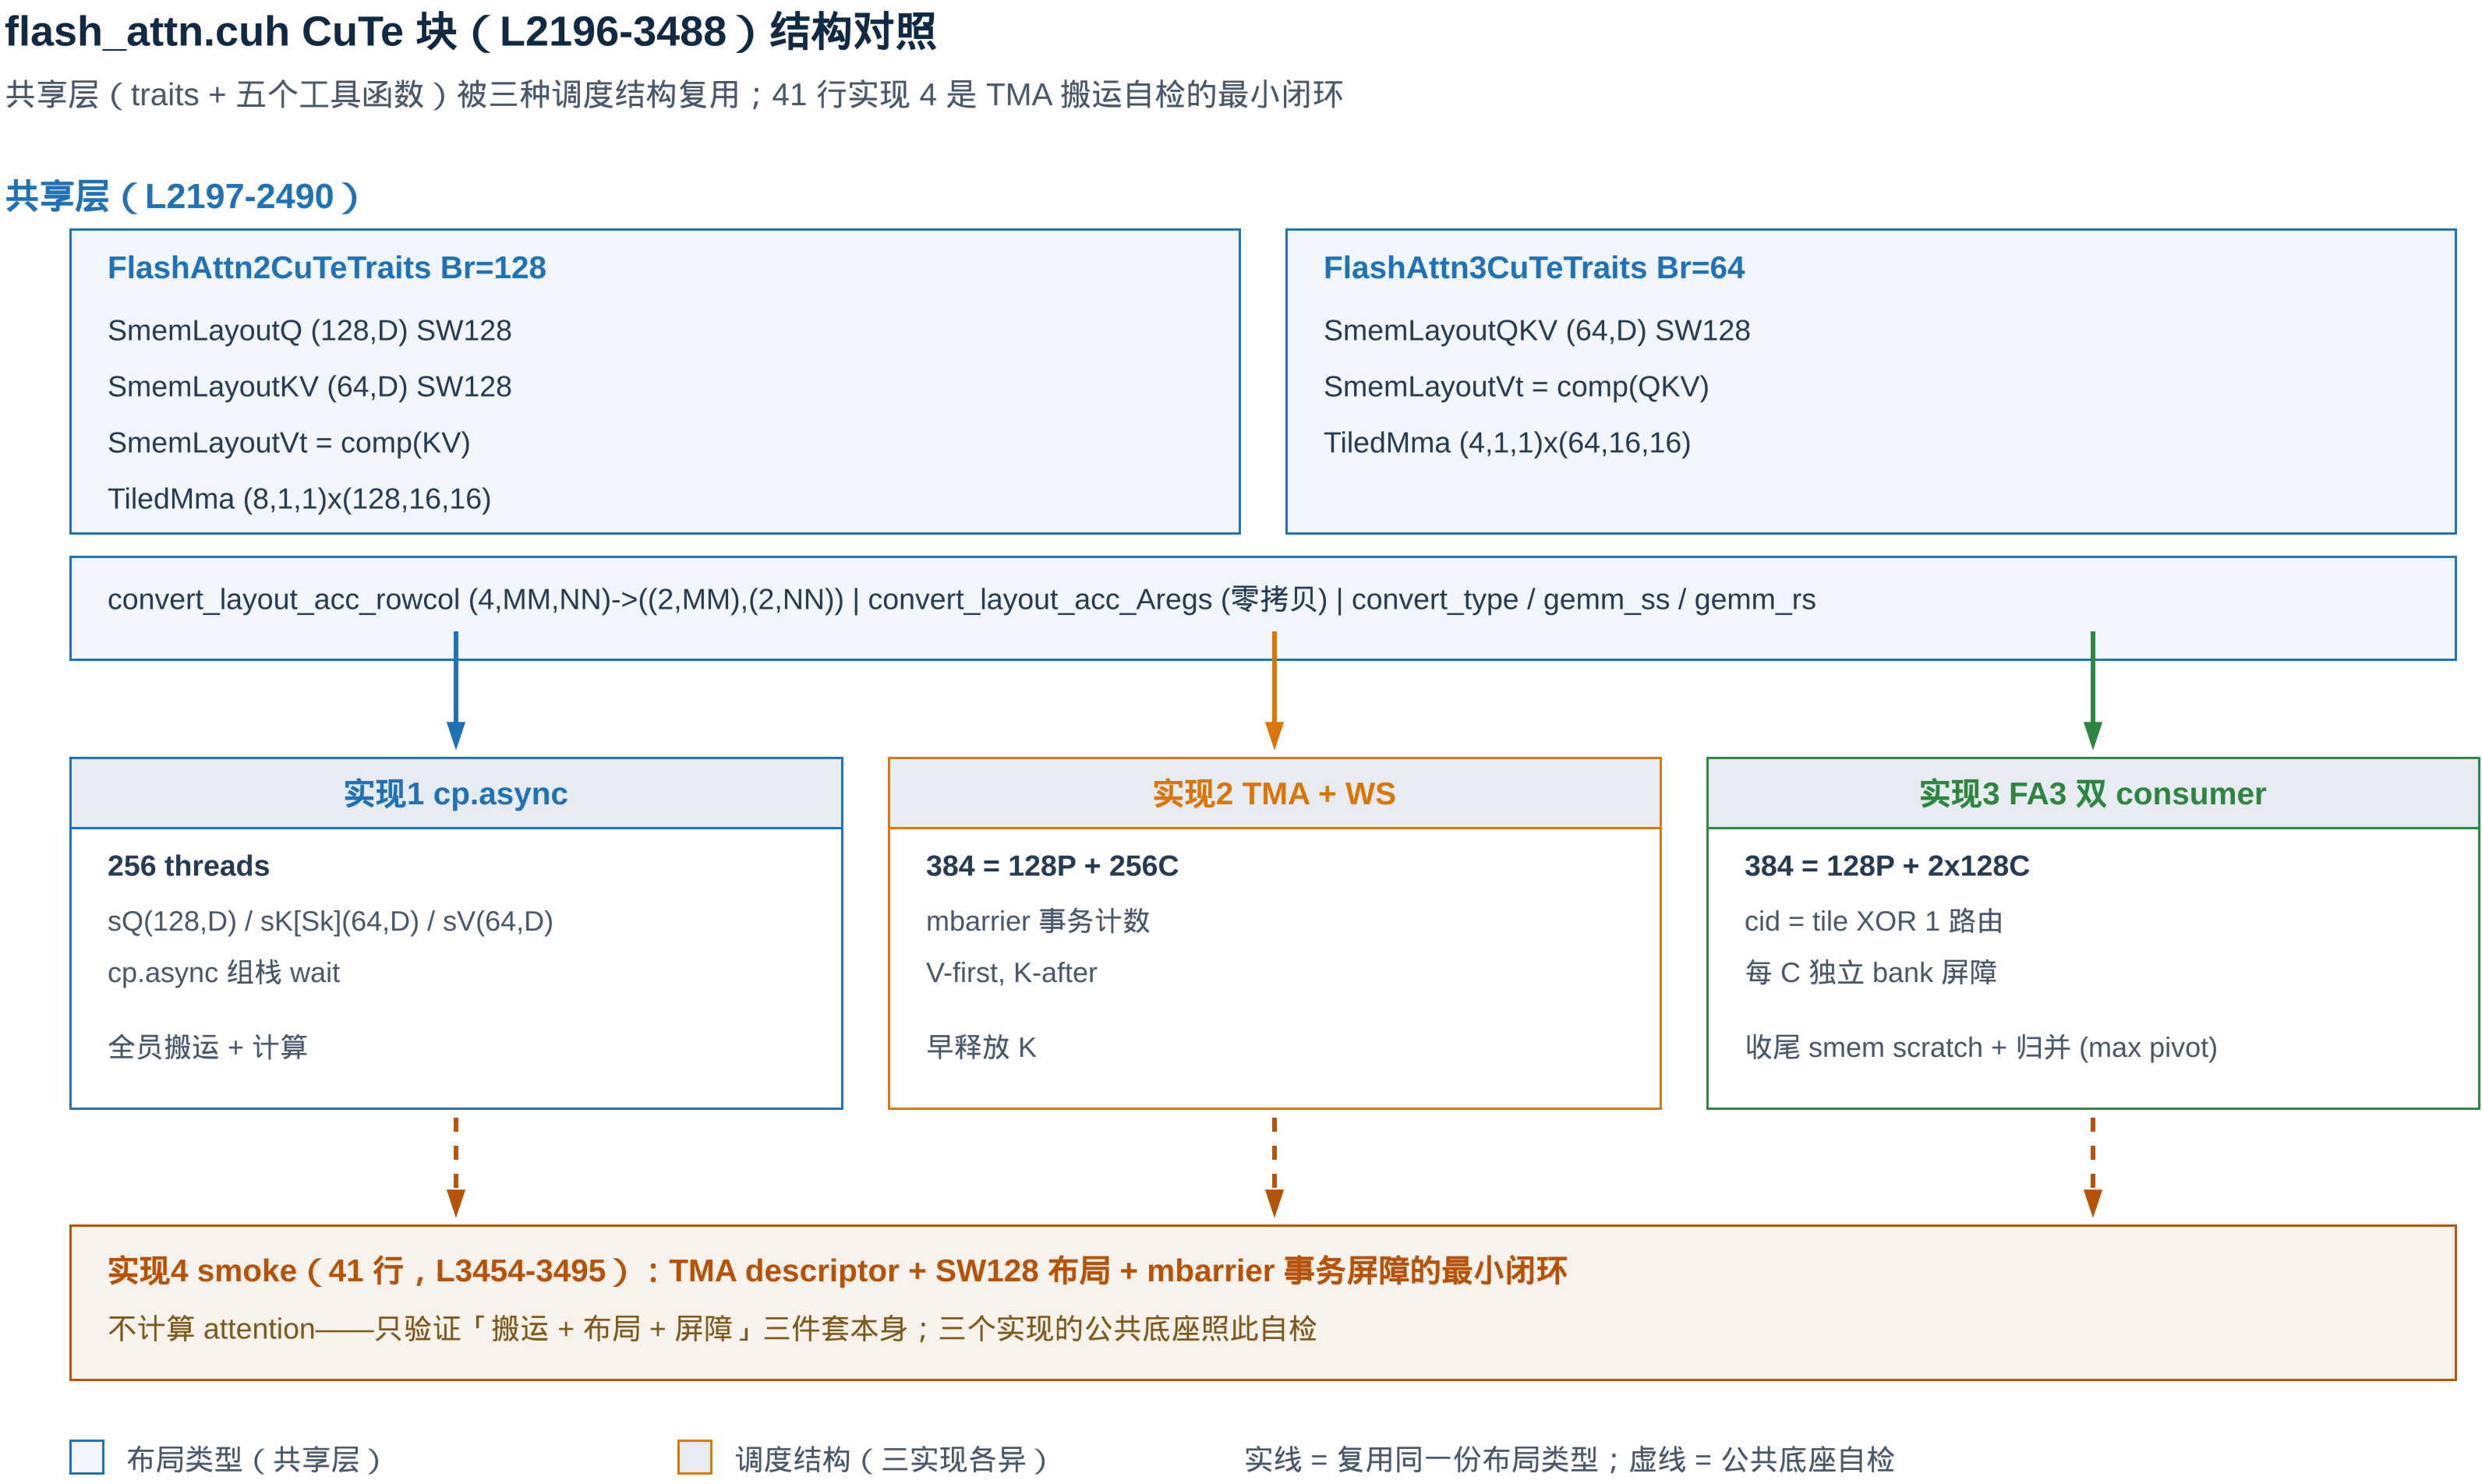
\includegraphics[width=0.98\textwidth]{figures/drawio/fig-25-1-cute-struct/fig-25-1.png}
\begin{tikzpicture}[font=\tiny, >=Stealth,
  secl/.style={font=\bfseries\fontsize{4.6}{5.2}\selectfont, inner sep=1pt},
  code/.style={font=\ttfamily\fontsize{4.2}{4.8}\selectfont, inner sep=1pt, anchor=west},
  sub/.style={font=\fontsize{4.2}{4.8}\selectfont, inner sep=1pt, anchor=west,
    align=left, text width=4.30cm},
  tcard/.style={draw=tkBlue, fill=tkFillBlue, inner sep=3pt},
  ihdr/.style={draw, fill=gray!14, align=center, inner sep=2pt,
    font=\bfseries\fontsize{4.4}{5}\selectfont},
]
  \node[secl, text=tkBlue, anchor=west] at (0,0.34) {共享层（L2197-2490）：traits + 五个工具函数};
  % 共享层：两个 traits 卡
  \draw[tcard] (0,-0.02) rectangle (7.00,-1.78);
  \node[code, text=tkBlue] at (0.10,-0.22) {\textbf{FlashAttn2CuTeTraits<D>}\ \ Br=128};
  \node[code] at (0.10,-0.56) {SmemLayoutQ\ \ (128,D)\ SW128};
  \node[code] at (0.10,-0.84) {SmemLayoutKV\ (64,D)\ SW128};
  \node[code] at (0.10,-1.12) {SmemLayoutVt\ = comp(KV)};
  \node[code] at (0.10,-1.40) {TiledMma\ \ (8,1,1)$\times$(128,16,16)};
  \draw[tcard] (7.50,-0.02) rectangle (14.50,-1.78);
  \node[code, text=tkBlue] at (7.60,-0.22) {\textbf{FlashAttn3CuTeTraits<D>}\ \ Br=64};
  \node[code] at (7.60,-0.56) {SmemLayoutQKV (64,D) SW128};
  \node[code] at (7.60,-0.84) {SmemLayoutVt\ = comp(QKV)};
  \node[code] at (7.60,-1.12) {TiledMma\ \ (4,1,1)$\times$(64,16,16)};
  % 共享层：工具函数横条
  \draw[tcard] (0,-1.95) rectangle (14.50,-2.55);
  \node[code] at (0.60,-2.25) {convert\_layout\_acc\_rowcol (4,MM,NN)$\to$((2,MM),(2,NN))};
  \draw[tkBlue!45, thin] (5.55,-2.00) -- (5.55,-2.50);
  \node[code] at (5.80,-2.25) {convert\_layout\_acc\_Aregs（零拷贝）};
  \draw[tkBlue!45, thin] (10.05,-2.00) -- (10.05,-2.50);
  \node[code] at (10.30,-2.25) {convert\_type\ /\ gemm\_ss\ /\ gemm\_rs};
  % 三个实现的调度结构卡（各自保持自己一层的调度色）
  \draw[draw=tkBlue, fill=white] (0,-3.00) rectangle (4.60,-5.00);
  \draw[draw=tkOrange, fill=white] (4.95,-3.00) rectangle (9.55,-5.00);
  \draw[draw=tkGreen, fill=white] (9.90,-3.00) rectangle (14.50,-5.00);
  \node[ihdr, text=tkBlue] at (2.30,-3.21) {实现 1：cp.async};
  \node[ihdr, text=tkOrange!85!black] at (7.25,-3.21) {实现 2：TMA + WS};
  \node[ihdr, text=tkGreen] at (12.20,-3.21) {实现 3：FA3 双 consumer};
  \node[sub] at (0.15,-3.66) {\textbf{256 threads}};
  \node[sub] at (0.15,-3.92) {sQ(128,D) / sK[$S_k$](64,D)};
  \node[sub] at (0.15,-4.18) {/ sV(64,D)};
  \node[sub] at (0.15,-4.44) {cp.async 组栈 wait<N>};
  \node[sub] at (0.15,-4.70) {全员搬运 $+$ 计算};
  \node[sub] at (5.10,-3.66) {\textbf{384 = 128P + 256C}};
  \node[sub] at (5.10,-3.92) {mbarrier 事务计数};
  \node[sub] at (5.10,-4.18) {V-first, K-after};
  \node[sub] at (5.10,-4.44) {早释放 K};
  \node[sub] at (10.05,-3.66) {\textbf{384 = 128P + 2$\times$128C}};
  \node[sub] at (10.05,-3.92) {cid = tile XOR 1 路由};
  \node[sub] at (10.05,-4.18) {每 C 独立 bank 屏障};
  \node[sub] at (10.05,-4.44) {收尾 smem scratch $+$ 归并};
  \node[sub] at (10.05,-4.70) {(max pivot)};
  % 共享层 -> 三实现（实线：复用同一份布局类型）
  \draw[->, tkBlue, semithick] (2.30,-2.60) -- (2.30,-2.96);
  \draw[->, tkOrange, semithick] (7.25,-2.60) -- (7.25,-2.96);
  \draw[->, tkGreen, semithick] (12.20,-2.60) -- (12.20,-2.96);
  % 实现 4：公共底座自检
  \node[draw=tkOrange!85!black, fill=tkFillOrange, align=center, inner sep=2pt,
    font=\fontsize{4.2}{4.8}\selectfont, text width=13.9cm]
    at (7.25,-5.80)
    {\textbf{实现 4 smoke（42 行，L3447-3488）：TMA descriptor $+$ SW128 布局 $+$ mbarrier 事务屏障的最小闭环}\\
     不计算 attention——只验证「搬运 $+$ 布局 $+$ 屏障」三件套本身；三个实现的公共底座照此自检};
  \draw[->, dashed, tkOrange, semithick] (2.30,-5.04) -- (2.30,-5.42);
  \draw[->, dashed, tkOrange, semithick] (7.25,-5.04) -- (7.25,-5.42);
  \draw[->, dashed, tkOrange, semithick] (12.20,-5.04) -- (12.20,-5.42);
  % 图例
  \fill[tkFillBlue, draw=tkBlue] (0.10,-6.60) rectangle (0.32,-6.82);
  \node[sub] at (0.42,-6.71) {布局类型（共享层复用）};
  \fill[gray!14, draw=tkOrange] (5.60,-6.60) rectangle (5.82,-6.82);
  \node[sub] at (5.92,-6.71) {调度结构（三实现各异）};
  \node[sub, text width=5.40cm] at (9.60,-6.71)
    {实线 $=$ 复用同一份布局类型；虚线 $=$ 公共底座自检};
\end{tikzpicture}
\caption{CuTe 块的四层结构：共享 traits 与五个工具函数（上），三个 attention
实现（中），以及 42 行的 TMA 搬运自检（底）。实线箭头表示同一份布局类型被
三种调度结构复用，虚线表示三个实现共用实现~4 的底座自检。}
\label{fig:25-1}
\end{figure}

\section{性能分析}

本节先交代源码注释里的既有数字与口径，再给本书的复测，最后汇总 CuTe 实测表。

先看源码注释。本章区间（L2196--3488）内\textbf{没有}任何 TFLOPS/加速比
断言：四个实现都是能跑对的对照样本，性能数字在相邻章节：
第~\ref{ch:16}~章区间内的 L61--71 注释给出 pad 与 XOR swizzle 的对照
（「约 120.0 TFLOPS，显著低于 Q/K/V kPad$=$8 的 166.6 TFLOPS」），
第~\ref{ch:17}~、\ref{ch:18}~章的性能节给出同机同批复测（RTX PRO 5000
sm\_120a、CUDA 13.2）。读这些数字时必须注意口径：$B{=}1,H{=}32$、
warmup$\ge$5、iters$\ge$20 取均值，FLOPS $=4BHN^2D$；
CuTe 版与手写版在\emph{同一口径}下才可比。

本书复测用的是本章测试（\texttt{book/\allowbreak{}tests/\allowbreak{}ch25\_\allowbreak{}fa\_\allowbreak{}cute.\allowbreak{}cu}），
\texttt{bench} 子命令按与第~\ref{ch:17}/\ref{ch:18}~章相同的口径测量
CuTe 实现 1/2 的吞吐：$B{=}1$、$H{=}32$、warmup$=5$、iters$=20$，
$D\in\{64,128\}$、$N\in\{4096\}$。三点预期：(1) 实现 1 与实现 2 的差异
是\textbf{搬运路径}（cp.async 全员搬 vs TMA 单线程发）而非计算，
$D{=}128$ 的 Q tile 更大（$128\times128$ 个 half $=32$\,KB），
实现 1 的 G2S 负载更重，两者差距应主要体现在大 $D$；
(2) 实现 3（双 consumer）与第~\ref{ch:18}~章手写 FA3 在 $B_r{=}64$ 上的
结构性差异只有谁搬，可对照式~\ref{eq:18-smem} 的 smem 占用；
(3) 本章全部实现是\textbf{非 causal、无 GQA/varlen} 的 self-attention，
与手写版限制相同（源码注释 L2528--2529 明示），因此这些数字只能说明
CuTe 化不牺牲性能，不能当作实现之间谁更快的定论。

CuTe 实测见表~\ref{tab:ch25-perf}：
\texttt{leetcuda\_\allowbreak{}bench\_\allowbreak{}sm120a.\allowbreak{}bin}
\texttt{--bench --bench-all} 的 FA CuTe 实测（RTX PRO 5000，sm\_120、110 SM、
CUDA 13.2；$B{=}1$、$H{=}32$、$N{=}8192$、$D{=}128$ dense，全部 F32Acc，
参照 cuDNN f32 的 230.2 TFLOPS）。

\begin{table}[H]
\centering
\caption{FA CuTe 实测（RTX PRO 5000，B=1 H=32 N=8192 D=128）}
\label{tab:ch25-perf}
\footnotesize
\setlength{\tabcolsep}{4pt}
\begin{tabular}{lrr}
\toprule
Kernel & Max Err & TFLOPS/cuDNN（加速比） \\
\midrule
FA2 CuTe MMA Stages (Sk=1, F32Acc) & 1.526e-05 & 184.4/230.2 (0.80x) \\
FA2 CuTe MMA Stages (Sk=2, F32Acc) & 1.526e-05 & 196.5/230.2 (0.85x) \\
FA2 CuTe TMA MMA WS (1 Consumer WG) (Sk=2, Sv=1, F32Acc) & 1.526e-05 & 218.6/230.2 (0.95x) \\
FA2 CuTe TMA MMA WS (1 Consumer WG) (Sk=3, Sv=1, F32Acc) & 1.526e-05 & 221.4/230.2 (0.96x) \\
\bottomrule
\end{tabular}
\end{table}

三个台阶清晰可见：实现 1 的 CuTe MMA Stages 已到 cuDNN 的 0.80--0.85$\times$，
纯 CuTe 抽象、无任何搬运特化就已接近厂商库；实现 2 的 CuTe TMA MMA WS 把
搬运与计算解耦后升到 0.95--0.96$\times$、逼近 cuDNN：TMA + warp
specialization 这条路线的收益在 CuTe 版上完整复现。再把 K 的 stage 从 2 加深到
3 只带来约 1.3\% 的提升（218.6 $\to$ 221.4 TFLOPS），流水深度的收益已边际递减；
更完整的 persistent-CTA WS 实现见第 26b 章。

\section{常见坑}

\textbf{坑一：K/V 的 \texttt{local\_tile} 坐标是打包维上的全局 tile 号。}
TMA tensor 的 shape 是 $[B\!\cdot\!H\!\cdot\!N, D]$，K/V 的块坐标必须写
\texttt{blockIdx.y * kv\_tiles + tile}；漏掉偏移时所有 head 读同一份 K/V：
$H{=}1$ 的正确性测试全绿，$H{>}1$ 的精度却差两个量级（源码 L2885--2892
的注释即为此事）。正确性测试必须包含 $H{\ge}2$（本章测试取 $H{=}2$）。

\textbf{坑二：\texttt{cp.\allowbreak{}async.\allowbreak{}wait\_\allowbreak{}group} 是 per-thread 的。}
它只保证\emph{本线程}提交的组完成；跨线程可见性仍要
\texttt{\_\allowbreak{}\_\allowbreak{}syncthreads\allowbreak{}()}。实现 1 里每一处 \texttt{wait} 后面都跟着一次
同步，不是冗余。省掉同步的版本可能在 $B_r{=}128$ 的负载下偶发错数据
（写入 smem 的线程与读取的线程不同）。

\textbf{坑三：V 是单 buffer，PV 之后必须同步才能进入下一轮。}
L2769 的 \texttt{\_\allowbreak{}\_\allowbreak{}syncthreads\allowbreak{}()} 注释写明「ldmatrix V 完成后才能覆盖
V smem」。删掉它，下一轮 3a 的 V cp.async 可能覆盖本轮尚未读完的 sV，
表现是间歇性数值错误，且只在 $D$ 大（ldmatrix 更多）时暴露。

\textbf{坑四：推导 B fragment 的寄存器布局时要用 nonswizzle 视图。}
\texttt{partition\_\allowbreak{}fragment\_\allowbreak{}B(sVt)} 若传入带 swizzle 的 \texttt{Smem\allowbreak{}Layout\allowbreak{}Vt}，
CuTe 推导 \texttt{ldmatrix.\allowbreak{}trans} 的线程-数据映射时会与 swizzle composition
冲突（源码 L2886--2893 与 L3010--3020 的两处注释）。正确做法是
\texttt{get\_\allowbreak{}nonswizzle\_\allowbreak{}portion}（寄存器布局与 smem 物理 swizzle 无关），
而 \texttt{partition\_S}（S2R copy 的源）仍用带 swizzle 的视图；两者
分工不能互换。

\textbf{坑五：\texttt{K} 的预取深度与尾部退化。}
$kStagesK>1$ 时 K 的预取位置是 \texttt{tile + kStagesK - 1}，尾部
$kStagesK{-}1$ 个 tile 不预取；此时栈里只剩 V 组，PV 前的 \texttt{wait<1>}
必须退化为 \texttt{wait<0>}（L2748--2753）。漏掉这个分支，尾部两个 tile
会等一个不存在的组，行为是等很久后照样算完（组计数不会变负），
但流水被拖成同步。

\textbf{坑六：\texttt{convert\_\allowbreak{}layout\_\allowbreak{}acc\_\allowbreak{}Aregs} 依赖 $m16n8k16$ 约定。}
式~\eqref{eq:25-aregs} 的 C 的后 2 值 $\leftrightarrow$ A 的 K 向连续 2 值
是 $m16n8k16$ 的 fragment 约定的推论，源码 L2360--2362 特意标注「不是通用
性质」。换 atom（如 $k8$ 或 wgmma）必须重推；照抄会得到静默错数据。

\textbf{坑七：P 的类型转换与布局重解释的先后顺序。}
正确顺序是 \texttt{convert\_\allowbreak{}type\allowbreak{}<Element>\allowbreak{}(t\allowbreak{}Cr\allowbreak{}S)} 再做
\texttt{convert\_\allowbreak{}layout\_\allowbreak{}acc\_\allowbreak{}Aregs}（实现 1 的 L2762--2766）：
\texttt{convert\_\allowbreak{}type} 用 \texttt{Numeric\allowbreak{}Array\allowbreak{}Converter} 按\emph{当前}
layout 的连续段做向量化转换，先改布局会让转换作用于错误的元素分组。

\textbf{坑八：f32 累加与 exp2 的缩放折叠。}
三处实现都写 \texttt{scale = rsqrtf(D) * M\_LOG2E}、用
\texttt{exp2f\allowbreak{}(s*scale - nxt)} 替代 \texttt{expf}：把 $1/\sqrt{D}$ 折进
$\log_2 e$ 既省一条乘法也让 SFU 走 \texttt{ex2.approx}。改动缩放因子时
必须同步改 \texttt{row\_\allowbreak{}max/\allowbreak{}\_\allowbreak{}sum} 的语义（它们都在 $\log_2$ 域），
否则 softmax 的归一化在数值上自洽但语义漂移。

\section{面试要点速查}

\textbf{Q1：CuTe 版 FlashAttention 消掉的到底是什么？}\\
A：消掉的是与调度正交的\emph{布局算术}：smem swizzle 的地址、ldmatrix 的
lane 映射、fragment 的寄存器编号、S$\to$P 的重解释。没有消掉的是
\emph{调度}：流水深度、屏障协议、释放时机（25.4.6 节）。CuTe 让 attention
变简单的准确说法是：简单在改 tile 不改正文，难的部分（等谁、何时释放）原样
保留。

\textbf{Q2：为什么 FA2 的 traits 用 8 个 warp、FA3 用 4 个？}\\
A：$B_r$ 不同（128 vs 64）。TiledMMA 的 AtomLayout 必须恰好铺满 $M$ 向
atom 数：$\langle16,8,16\rangle\otimes\langle8,1,1\rangle$ 的 $M$ 是 128，
$\langle4,1,1\rangle$ 的 $M$ 是 64。若 warp 数与 tile 不匹配，
\texttt{partition\_\allowbreak{}fragment\_\allowbreak{}C} 仍能编译，但会有 warp 拿到空 fragment
（静默低效）。

\textbf{Q3：\texttt{convert\_\allowbreak{}layout\_\allowbreak{}acc\_\allowbreak{}rowcol} 之后为什么是 4-lane 归约？}\\
A：$m16n8$ 的 C fragment 里，同一行的 2 个片段分布在 lane $\bmod 4$ 的
不同值上（式~\eqref{eq:25-rowcol-num} 的 $(2,1)$ 结构）；两次
\texttt{\_\allowbreak{}\_\allowbreak{}shfl\_\allowbreak{}xor\_\allowbreak{}sync}（步长 1、2）把宽度 4 的子组归约完，
再乘以每线程的列数即可。宽了会重复计数、窄了会漏行。

\textbf{Q4：P 为什么会零拷贝地变成 A 操作数？}\\
A：因为 $B_c$（S 的列）与 $PV$ 的 K 维是同一个物理维度，$m16n8k16$ 的
C 与 A 在该维度上的 2 元素的对应方式恰好兼容（式~\eqref{eq:25-aregs}）。
这是寄存器复用的经典技巧，CuTe 用一次 \texttt{logical\_\allowbreak{}divide} 表达，
代价是把它从技巧变成了有条件的等式，条件写在注释 L2360--2362。

\textbf{Q5：实现 2 的 V 为什么在 K 之前发 TMA？}\\
A：等待顺序是先 K 后 V（QK 需要 K、PV 需要 V），但\emph{发射}顺序是
V 先：V 的落盘窗口要横跨 QK+softmax 两段计算。这与实现 1 的
V 最后发、等 wait<1> 形异实同：都是让 V 的延迟藏在 softmax 里。

\textbf{Q6：四个实现里哪个最快？}\\
A：本章不做这个断言（25.6 节）：四者的 tile、线程、流水深度都不同，
受控对照需要在同一 $B_r/B_c/kStages$ 下比较。可确认的是：
CuTe 化没有牺牲吞吐（对照第~\ref{ch:17}/\ref{ch:18}~章复测）。

\textbf{Q7：TMA 的 mbarrier 协议里，phase 为什么每回绕一轮翻转？}\\
A：mbarrier 是相位对象而非计数器：arrive 数到零后相位翻转、
计数重置。stage 循环复用同一个 barrier 时，$t$ 号 tile 属于第
$\lfloor t/S\rfloor$ 个相位，故 phase $=$ 该商 $\bmod\ 2$
（图~\ref{fig:25-proto}）。写错 phase 的症状是等一个已经过去的相位：
永久挂起或提前通过。

\textbf{Q8：smoke kernel 为什么值得单独存在？（42 行）}\\
A：它是 TMA + SW128 布局 + 事务屏障三件套的最小闭环，把
\emph{搬运链路}与\emph{计算链路}解耦。调 attention 时先用它排除
搬运侧问题（descriptor 参数、box 与 layout 匹配、arrive\_tx 的字节数），
再去查计算侧；本章测试（25.9 节）的三个 case 全走实现 1，并未单独
驱动 smoke kernel；需要验搬运链路时可把它当独立小用例编译运行。

\section{最小测试与动手实验}

测试文件：\texttt{book/\allowbreak{}tests/\allowbreak{}ch25\_\allowbreak{}fa\_\allowbreak{}cute.\allowbreak{}cu}。三个 case 全部是
\textbf{端到端正确性}验证：固定 $B{=}1$、$H{=}2$、$k_{StagesK}{=}2$，全部
调用实现 1（cp.async 统一流水，256 线程），与 CPU fp64 参考
$\mathrm{softmax}(QK^\top/\sqrt{D})V$ 对照（half 输入/输出），容差
\texttt{TOL\_F16ACC}$=5\times10^{-2}$。形状约束：$N\bmod 128=0$
（$B_r{=}128$）且 $N\bmod 64=0$（$B_c{=}64$）、$D\in\{64,128\}$
（kernel 的 \texttt{static\_assert}；sm$_{80}+$）。三个形状的分工：

\begin{itemize}
  \item \textbf{case A（$D{=}64$，$N{=}128$）}：单 Q tile、KV 分 2 段，
        以最小形状走通完整的 online softmax KV 循环；
  \item \textbf{case B（$D{=}64$，$N{=}256$）}：多 Q tile，grid $(2,2)$
        （Q 方向 2 tile $\times$ $B{\cdot}H{=}2$），验证
        \texttt{local\_tile} 切分与 grid 映射；
  \item \textbf{case C（$D{=}128$，$N{=}128$）}：大 $D$ 路径，smem
        80\,KB $<$ 99\,KB optin，验证 traits 在 $D{=}128$ 下的 smem 预算
        与 fragment 形状。
\end{itemize}

host 端的 traits 结构断言（\texttt{tile\_\allowbreak{}size\_\allowbreak{}mnk}、fragment
形状、D-chunk 语义）与 TMA 往返 smoke 不在本测试内：前者由第~\ref{ch:22}~章
与第~\ref{ch:26}~章的最小测试承载，后者即本章实现 4 的 42 行 smoke kernel，
可单独编译驱动。

编译与运行（本机 sm\_120a，6 号卡；结果见下）：

{\footnotesize
\begin{lstlisting}[style=console]
$ cd book/tests && CUDA_VISIBLE_DEVICES=6 ./build_tests.sh --arch sm_120a --ch ch25
== ch25_fa_cute.cu (sm_120a)
PASS fa_cute cp.async D=64 Sk=2 B=1 H=2 N=128: max_abs_err=8.149e-05 (tol=5.0e-02)
PASS fa_cute cp.async D=64 Sk=2 B=1 H=2 N=256: max_abs_err=6.614e-05 (tol=5.0e-02)
PASS fa_cute cp.async D=128 Sk=2 B=1 H=2 N=128: max_abs_err=8.084e-05 (tol=5.0e-02)
ALL OK
\end{lstlisting}
}

动手实验建议：（1）把 case B 的 $H$ 改成 1、并把 kernel 换成实现 2
（需 \texttt{NOTES\_\allowbreak{}V2\_\allowbreak{}ENABLE\_\allowbreak{}TMA\_\allowbreak{}MMA\_\allowbreak{}WS}），再删掉实现 2 producer 的
\texttt{blockIdx.y * kv\_tiles} 偏移，正确性仍全绿，说明单 head
测试会掩蔽多 head 缺陷；（2）把实现 1 的模板参数从
\texttt{<64, 2>} 改成 \texttt{<64, 3>} 并打印 smem 用量，观察 K 三级时
smem 增量的构成（V 仍单 buffer）；（3）把 case A 的模板参数从
\texttt{<64, 2>} 改成 \texttt{<96, 2>}，观察 traits 的
\texttt{static\_\allowbreak{}assert\allowbreak{}(k\allowbreak{}Head\allowbreak{}Dim =\allowbreak{}=\allowbreak{} 64 || =\allowbreak{}=\allowbreak{} 128)} 拒绝编译，
再对照第~\ref{ch:26}~章 FFPA 的 \texttt{kHeadDim \% 64 == 0} 放宽条件；
（4）把实现 2 的 \texttt{kStagesK} 从 1 调到 2，核对 smem 是否仍在
sm\_120a 的 99\,KB optin 之内（$D{=}128$ 时 Q 一段就占 32\,KB）。



\section*{延伸阅读}

\begin{itemize}
  \item @竹熙佳处《写给大家看的 CuTe 教程：Layout Compose \& Inverse》\\
        \url{https://zhuanlan.zhihu.com/p/1962625273636845008}\\
        （$S\to P$ 布局变换的两种讲法：Tri Dao 的几何重排与 @reed 的
        inverse$\circ$compose 代数法，本章 25.3.4 节的主参考）；
  \item @reed《cute 之 简单 GEMM 实现》与《cute 之 高效 GEMM 实现》\\
        \url{https://zhuanlan.zhihu.com/p/667521327}\\
        \url{https://zhuanlan.zhihu.com/p/675308830}\\
        （Tensor $\to$ 分块 $\to$ 划分 $\to$ 拷贝 $\to$ 计算的组装范式、
        多级流水写法与 Epilogue 的来龙去脉；前者是本章实现 1 的蓝本，
        后者的四个高效是三级搭建的对照读物）；
  \item @竹熙佳处《写给大家看的 CuTe 教程：tiled mma》\\
        \url{https://zhuanlan.zhihu.com/p/1937145378446226159}\\
        （fragment 视角的 mma 线程-值映射，25.3.2--25.3.4 节的入门读物）；
  \item @66RING《使用 cutlass cute 复现 flash attention》\\
        \url{https://zhuanlan.zhihu.com/p/696323042}\\
        （CuTe 版 attention 的另一种组织：把 Q/K/V 的 smem 布局与 S2R copy
        全部交给 CuTe，25.3 节的类型推导链可与之互证）；
  \item @shengying.wei《FlashAttention 笔记：tiny-flash-attention 解读》\\
        \url{https://zhuanlan.zhihu.com/p/708867810}\\
        （极简 FA 实现里 MMA atom 与线程布局的选择逻辑，对应式~\eqref{eq:25-eurepeat}
        的另一种推导）；
  \item @Titus《GEMM 流水线：single/multi-stage、pipeline》\\
        \url{https://zhuanlan.zhihu.com/p/712451053}\\
        （软件流水的 stage 语义；25.3.5 节组栈 vs 事务计数两种等待模型的
        对照背景）；
  \item @竹熙佳处《写给大家看的 CuTe 教程：async pipeline》\\
        \url{https://zhuanlan.zhihu.com/p/2024832248386528275}\\
        （CuTe 里表达异步流水的最新手法，可与实现 1 的手写组栈用法并读）。
\end{itemize}

% ch26-cute-ffpa.tex — 撰写任务见 RFC.md F7
\chapter{CuTe 应用（三）：FFPA Split-D 的类型代数}\label{ch:26}

\section{本章导读}

第~\ref{ch:19}~章把 Split-D 当作\emph{算法}讲透了：为什么大 head\_dim 会触及
smem 容量上限、$S$ 如何沿 $D$ 切成 chunk、$O$ 如何拆成分量并在收尾合并、chunk 数与
流水级数的相位关系如何推导。本章换一个视角：把同一份代码（\texttt{ffpa\_\allowbreak{}attn.\allowbreak{}cuh}
的 CuTe 版）当作\emph{类型系统}来读，回答一个第~\ref{ch:19}~章刻意没有展开的问题：

\begin{quote}
  Split-D 的每一个结构决策（双 TiledMma、chunk 循环、独立 $O$ 累加器），
  在 CuTe 里究竟长什么\emph{类型}？哪些事实可以在 host 端离线断言，
  而不必等到 device 上跑出错误结果？
\end{quote}

这个视角有直接的工程收益。第~\ref{ch:25}~章已经演示过一次：手写 attention 里靠注释和
规则维持的 lane 映射、tile 计数、转置视图，在 CuTe 版里变成了
\texttt{print\allowbreak{}(layout)} 可以打印、\texttt{static\_\allowbreak{}assert} 可以断言、host 端
测试可以离线核对的\emph{类型事实}。FFPA 把这件事推得更远一步：Split-D 引入的
chunk 循环让归约维度被切开这件事也必须落在类型上：

\begin{itemize}[itemsep=2pt,topsep=2pt]
  \item QK 与 PV 用\emph{两个不同形状}的 TiledMma，却共享同一批 128 个线程；
        两个 fragment 为什么能免 smem 交接？
  \item $S$ 的归约维（$D$）被切成 $C$ 个 chunk，但 $S$ 的 fragment 形状
        \emph{一次都没有变}，chunk 循环到底切开了什么？
  \item 每个 chunk 一份 $O$ 累加器，$C\times 32$ 个 f32 逻辑累加值是怎么被
        类型推导出来的？
\end{itemize}

本章的叙述顺序与第~\ref{ch:25}~章一致：先给类型代数（26.3 节，所有公式都能
在 host 端用 CuTe 原语验证），再逐相位读 kernel（26.4 节），最后是常见坑、
面试速查与最小测试。全章沿一条数据流展开：Q/K 的 chunk 从 smem
切片进来、在 $S$ 的 32 个寄存器里跨 chunk 累加、经 rowcol 视图做 online
softmax 就地写回 $S$，再由 \texttt{convert\_type} 产生 f16 fragment、用 Aregs
重解释成 PV 的 A 操作数。每一步都只用
\emph{类型}回答数据在哪、什么形状、谁持有。两处布局变换（rowcol 与
Aregs）的通用讲法在第~\ref{ch:25}~章 25.3.4 节已经展开，本章只补 Split-D
语境下的增量。涉及算法推导（chunk 分解的数学、online softmax 的不变量、
相位计数）的地方，直接引用第~\ref{ch:19}~章，不重复。

前置：第~\ref{ch:19}~章（Split-D 算法）、第~\ref{ch:20}--\ref{ch:22}~章
（布局代数、TiledCopy、TiledMMA）、第~\ref{ch:25}~章（attention 的 CuTe 化，
包括共享层 \texttt{convert\_\allowbreak{}layout\_\allowbreak{}acc\_\allowbreak{}rowcol} 与 \texttt{convert\_\allowbreak{}layout\_\allowbreak{}acc\_\allowbreak{}Aregs}
的来历）。

\section{问题与动机}

Split-D 的动机在源头注释里写得很直白（\texttt{ffpa\_\allowbreak{}attn.\allowbreak{}cuh} L7--8）：
\textbf{支持 head\_dim $>128$ 的 large head-dim attention，通过 64-wide Split-D
chunks 处理}。第~\ref{ch:19}~章量化了为什么必须分：smem 容量、以及
$\mathrm{softmax}$ 的结构性位置。本节只关心分完之后抽象层多出的四个问题。

先从第~\ref{ch:25}~章的结论出发。FA2 的三个 CuTe 实现里，attention 的
$D$ 维（head\_dim）是\emph{一个整体}：Q/K/V 的 smem tile 直接是
$[B_r, D]$、$[B_c, D]$，TiledMma 的 $K$ 向一次覆盖 16 列，循环在 $N$（KV tile）
方向滚动。FFPA 把这两件事都改了：

\begin{enumerate}[itemsep=3pt,topsep=3pt]
  \item K 向（$D$）被切成 chunk，循环滚动。$D=512$ 时
        $C = 512/64 = 8$ 个 chunk；QK 的累加变成一个\emph{跨 chunk 的求和}，
        每个 chunk 内部仍是一条标准的 $k16$ MMA 链。
  \item QK 与 PV 的 TiledMma 形状不同。QK 要一次覆盖 $S[64,64]$
        （省掉 N-tile 循环），PV 每次只覆盖 $O$ 的 16 列，
        以缩小单次调用的 C fragment 与临时量；跨 chunk 的 $O$ 总量仍由
        $D$ 与线程数决定。两者共享同一批线程，$S$（QK 的 C fragment）必须
        变成 $P$（PV 的 A 操作数）。
  \item $O$ 的累加器按 chunk 分裂。$D=512$、$C=8$ 时，每个线程
        持有 $8\times32$ 个 f32 的 $O$ 分量。
  \item 生产者也要跟着分 chunk。TMA box 或 cp.async 的搬运单元
        从整块 $[64,D]$ 变成 $C$ 个 $[64,64]$。
\end{enumerate}

四个问题的共同点：它们\emph{都不是数值问题}（数值精度与归约顺序都已确
定），而是\textbf{类型与布局问题}：tile 怎么切、fragment 怎么换解释、寄存器
怎么编号、循环与 stage 怎么对应。把这四个问题逐个翻译成 CuTe 的类型与布局，
就是用 CuTe 抽象表达 Split-D 的全部内容。

本章引用的源码位置汇总在表~\ref{tab:26-code}。

\begin{table}[htbp]
\centering
\caption{本章引用的 \texttt{ffpa\_\allowbreak{}attn.\allowbreak{}cuh} 位置（CuTe 版，cp.async 路径
\texttt{ffpa\_\allowbreak{}split\_\allowbreak{}d\_\allowbreak{}cute}，L79--376）。TMA+WS 版在同构位置复用同一批
helper，差异归第~\ref{ch:19}~章。}
\label{tab:26-code}
\begin{tabular}{p{4.2cm}p{3.4cm}p{6.0cm}}
\toprule
源码位置 & 内容 & 本章视角 \\
\midrule
L42--61 & traits：smem 布局与双 TiledMma & 类型推导链（26.3.1） \\
L79--97 & kernel 签名与 chunk 常量 & 128 线程 / \texttt{kDChunks}（26.4.1） \\
L118--128 & G2S \texttt{TiledCopy} & TV 布局与 MMA 对齐（26.4.2） \\
L136--141 & V 的 fragment 布局预计算 & 转置视图与 nonswizzle（26.4.3） \\
L152--176 & fragment 尺寸与寄存器占用 & 可断言的常量（26.3.2） \\
L217--271 & Phase 1：QK 的 chunk 流水 & 归约维的循环表达（26.4.5） \\
L273--303 & Phase 2：softmax 与 $P$ 的生成 & rowcol 与 Aregs（26.3.3） \\
L307--353 & Phase 3：PV 的 chunk 循环 & 双 TiledMma 的交接（26.4.6） \\
L355--374 & Phase 4：归一化与写回 & 收尾的布局复用（26.4.7） \\
\bottomrule
\end{tabular}
\end{table}

\section{数学原理：类型与布局代数}

\subsection{两个 TiledMma 的推导链}

第~\ref{ch:22}~章给出了 TiledMMA 的三元组
$(\mathrm{Atom},\ \mathrm{AtomLayout},\ \mathrm{Tile})$，以及每线程补足的
atom 重复数（源码注释称之为 \texttt{EURepeat}）：

\begin{equation}
  \mathrm{EURepeat} \;=\; \frac{\mathrm{Tile}}
  {\mathrm{AtomShape}\otimes \mathrm{AtomLayout}} ,
  \qquad
  \mathrm{AtomShape} = (16,8,16),\quad \mathrm{AtomLayout} = (4,1,1).
  \label{eq:26-eurepeat}
\end{equation}

代入两个 Tile（\texttt{ffpa\_\allowbreak{}attn.\allowbreak{}cuh} L52--58）：

\begin{align}
  \text{QK:}\quad & (64,64,16) \oslash \bigl((16,8,16)\otimes(4,1,1)\bigr)
    = (64,64,16)\oslash(64,8,16) = \langle 1,8,1\rangle ,
  \label{eq:26-qk}\\[2pt]
  \text{PV:}\quad & (64,16,16) \oslash (64,8,16) = \langle 1,2,1\rangle .
  \label{eq:26-pv}
\end{align}

读法：$M$ 向的 4 个 atom 位置被 4 个 warp 分完（$\mathrm{AtomLayout}$ 的
$M$ 分量 $=4$，每 warp 负责 16 行，故 $M$ 向的重复数为 1）；$N$ 向没有
atom-layout 的分工（$N$ 分量 $=1$），所以 $N$ 向的重复数就是
$\mathrm{Tile}_N/8$：QK 是 8，PV 是 2。

\begin{quote}
  $\mathrm{EURepeat}_N$ 就是每个线程每个 k-step 发射的
  \texttt{mma.sync} 条数。\allowbreak{}QK 的 8 条一次覆盖 $S$ 的整个 64 列
  （$8\times n8$），于是 N-tile 循环整个消失；PV 的 2 条覆盖单次调用的
  16 列。一个完整 O chunk 为 64 列，chunk 内先由 4 个 N-tile 覆盖，
  外层 V-chunk 循环再遍历后续各个 64 列 chunk。
\end{quote}

图~\ref{fig:26-dual-mma} 把这条对比摆成两个 tile 网格：行维同样被
$\mathrm{AtomLayout}=(4,1,1)$ 的 4 个 warp 分完，列维的 atom 数相差 4 倍。

\begin{figure}[H]
\centering
\begin{tikzpicture}[
  blknum/.style={font=\footnotesize\bfseries, inner sep=1pt},
  axl/.style={font=\scriptsize, inner sep=1pt},
]
  % 行轴：4 warp 分 M=64（AtomLayout=(4,1,1) 的 M 分量 = 4，每 warp 16 行）
  \foreach \wr/\mlo/\mhi in {0/0/15, 1/16/31, 2/32/47, 3/48/63} {
    \node[axl,anchor=east,align=right] at (1.02,-\wr*0.86-0.43)
      {w\wr\\{\tiny $m\,\mlo..\mhi$}};
  }
  % 左网格：S = QK 的输出 tile 64x64（4 warp 行块 x 8 个 n8 atom 列块）
  \foreach \wr in {0,...,3} {
    \foreach \aa in {0,...,7} {
      \pgfmathtruncatemacro{\gra}{12+8*\aa}
      \pgfmathtruncatemacro{\mn}{\aa+1}
      \fill[tkBlue!\gra] (1.1+\aa*1.05,-\wr*0.86) rectangle (1.1+\aa*1.05+1.05,-\wr*0.86-0.86);
      \node[blknum] at (1.1+\aa*1.05+0.525,-\wr*0.86-0.43) {\mn};
    }
  }
  \draw[thick, tkBlue] (1.1,0) rectangle (9.5,-3.44);
  \foreach \wr in {1,2,3} {
    \draw[very thick] (1.1,-\wr*0.86) -- (9.5,-\wr*0.86);
  }
  \foreach \aa in {1,...,7} {
    \draw[thin] (1.1+\aa*1.05,0) -- (1.1+\aa*1.05,-3.44);
  }
  % 右网格：O 的单次 PV 调用视图 64x16（4 warp 行块 x 2 个 n8 atom 列块）
  \foreach \wr in {0,...,3} {
    \foreach \aa in {0,...,1} {
      \pgfmathtruncatemacro{\gra}{18+30*\aa}
      \pgfmathtruncatemacro{\mn}{\aa+1}
      \fill[tkGreen!\gra] (11.0+\aa*0.95,-\wr*0.86) rectangle (11.0+\aa*0.95+0.95,-\wr*0.86-0.86);
      \node[blknum] at (11.0+\aa*0.95+0.475,-\wr*0.86-0.43) {\mn};
    }
  }
  \draw[thick, tkGreen] (11.0,0) rectangle (12.9,-3.44);
  \foreach \wr in {1,2,3} {
    \draw[very thick] (11.0,-\wr*0.86) -- (12.9,-\wr*0.86);
  }
  \draw[thin] (11.95,0) -- (11.95,-3.44);
  % 顶部标题与 atom 刻度
  \node[font=\scriptsize\bfseries,align=center,text=tkBlue] at (5.3,0.85)
    {QK TiledMma：Tile $=(64,64,16)$\\$\mathrm{EURepeat}=\langle 1,8,1\rangle$};
  \node[font=\scriptsize\bfseries,align=center,text=tkGreen!70!black] at (11.95,0.85)
    {PV TiledMma：Tile $=(64,16,16)$\\$\mathrm{EURepeat}=\langle 1,2,1\rangle$};
  \node[axl,anchor=south,text=tkBlue] at (5.3,0.22) {$S$（每块 = 一个 $n8$ atom，格内数字 = 该 warp 本 k-step 发射的第几条 \texttt{mma.sync}）};
  \node[axl,anchor=south,text=tkGreen!70!black] at (11.95,0.22) {$O$ 的单次 PV 调用视图};
  \foreach \aa in {0,...,7} {
    \node[axl,anchor=north] at (1.1+\aa*1.05+0.525,-3.52) {\aa};
  }
  \foreach \aa in {0,...,1} {
    \node[axl,anchor=north] at (11.0+\aa*0.95+0.475,-3.52) {\aa};
  }
  \node[axl,anchor=north] at (5.3,-3.95) {atom 列序（$N$ 向，每块 8 列：QK 共 $8{\times}8{=}64$ 列）};
  \node[axl,anchor=north] at (11.95,-3.95) {单视图共 16 列};
  % 交接箭头
  \draw[-{Stealth},thick,tkPurple] (9.72,-1.72) -- (10.78,-1.72);
  \node[font=\scriptsize,anchor=south,text=tkPurple] at (10.25,-1.66) {$P$};
  \node[font=\tiny,align=center,anchor=north,text=tkPurple] at (10.25,-1.78) {softmax\\Aregs 交接};
  % 底部两行注记
  \node[axl,anchor=north west,align=left,text width=11.6cm] at (1.1,-4.35)
    {两个完整输出的 frag 相同：$\mathrm{frag}_S=\mathrm{frag}_O=((2,2),1,8)=32$ 值/线程
     （式~\eqref{eq:26-frag32}，第三 mode 的 8 来历不同）；右侧仅画 O chunk 的一个 N-tile，};
  \node[axl,anchor=north west,align=left,text width=11.6cm] at (1.1,-5.25)
    {差别全在 $N$ 向：\textcolor{tkBlue}{QK} 的 $\mathrm{EURepeat}_N{=}8$ ——8 条 \texttt{mma.sync} 一次覆盖 $S$ 整个 64 列，\textbf{N-tile 循环}消失；
     \textcolor{tkGreen!70!black}{PV} 的 $\mathrm{EURepeat}_N{=}2$ 覆盖单视图的 16 列，完整 O chunk 内需 4 个 N-tile，外层 V-chunk 再推进 64 列。};
\end{tikzpicture}
\caption{双 TiledMma 的 Tile 分工（式~\eqref{eq:26-qk}--\eqref{eq:26-pv}）。
左：QK 的输出 $S[64,64]$——4 个 warp 各占 16 行（$\mathrm{AtomLayout}$ 的 $M$ 分量 4），
列向 8 个 $n8$ atom 由\textbf{同一线程}在一个 k-step 里连发 8 条 \texttt{mma.sync} 覆盖
（蓝深浅 8 档标识 atom 身份，格内数字为发射序）；右：PV 单次调用的输出视图为
$[64,16]$（绿 2 档、2 个 atom、2 条 \texttt{mma.sync}），完整 O chunk 为 $[64,64]$，
由 4 个这样的 N-tile 组成。中间箭头是 26.3.3 节的
交接：$S$ 经 softmax 后由 \texttt{convert\_type} 转成 f16 fragment，
\texttt{Aregs} 再重解释其布局作为 PV 的 A 操作数；全程不经过 smem。}
\label{fig:26-dual-mma}
\end{figure}

对照第~\ref{ch:25}~章 FA2 traits 的 $(8,1,1)\otimes(128,16,16)$：那里是
8 个 warp 分 $M=128$，$N$ 向重复数为 2。同一套公式，两种分工：FA2 把线程
堆在 $M$ 上换取更大的 $B_r$；FFPA 仍是 4 个 warp 分 $M=64$，$N$ 向没有
atom-layout 分工，一次覆盖整行块 $S$ 靠的是同一线程的
$\mathrm{EURepeat}_N=8$，不是把线程堆到 $N$ 上。

\subsection{fragment 的元素计数：两个恒等式}

TiledMma 定下来之后，每个线程持有多少寄存器就定了。这里有两个恒等式，后面
要讲的免 smem 交接就建立在它们上。

\textbf{恒等式一（C fragment 的大小）}：
\texttt{partition\_\allowbreak{}fragment\_\allowbreak{}C} 把\emph{目标输出形状}按 TiledMma 的线程布局
切开，所以

\begin{equation}
  \bigl|\mathrm{frag}_C\bigr| \;=\;
  \frac{\bigl|\text{目标输出形状}\bigr|}{\text{线程数}} .
  \label{eq:26-csize}
\end{equation}

FFPA 的两处调用（L152 与 L218）目标形状都是 $(64,64)$，线程数都是 128，
所以 QK 的 $S$ 与 PV 的 $O$ 都是每线程 32 个 f32。实测：

\begin{equation}
  \mathrm{frag}_S = \bigl((2,2),1,8\bigr) = 32\ \text{值/tid},\qquad
  \mathrm{frag}_O = \bigl((2,2),1,8\bigr) = 32\ \text{值/tid} .
  \label{eq:26-frag32}
\end{equation}

注意 $\mathrm{frag}$ 的第三 mode 是 8：那是 QK 的 $\mathrm{EURepeat}_N$
在 $S$ 上的投影。$O$ 的第三 mode 数字恰好也是 8，但它来自目标输出
$64$ 列按每个 $n8$ atom 分出的 $8$ 个列组（$64/8{=}8$），
不是 $\mathrm{EURepeat}_N$ 的 $8$。两个 32 的来历不同、大小相同，
这是 $S\to P$ 与 $P\to O$ 两条交接链路能成立的前提。

恒等式二（rowcol 视图的行列数）：online softmax 要在
行上做 max/sum，所以第~\ref{ch:25}~章的工具函数
\texttt{convert\_\allowbreak{}layout\_\allowbreak{}acc\_\allowbreak{}rowcol} 把 $C$ fragment 从
$(\mathrm{MMA}=4,\ \mathrm{MMA\_M},\ \mathrm{MMA\_N})$ 重排成
$\bigl((2,\mathrm{MMA\_M}), (2,\mathrm{MMA\_N})\bigr)$。FFPA 用它推两个
常量（L158--162）：

\begin{equation}
  \mathrm{nrow} = 2\cdot\mathrm{MMA\_M} = 2, \qquad
  \mathrm{ncol} = 2\cdot\mathrm{MMA\_N} = 16 .
  \label{eq:26-rowcol}
\end{equation}

$\mathrm{nrow}=2$ 的含义：\emph{每个线程只拥有 2 行}，行内 16 列。
$n16$ 的 $C$ fragment 里，一个线程的 4 个值的一半（行偏移 $+8$ 的那对）
属于另一行；4 个线程（lane 的 $\text{id}/4$ 相同、$\text{id}\bmod 4$ 不同）
拼成完整的一行，源码里行归约只用 \texttt{\_\allowbreak{}\_\allowbreak{}shfl\_\allowbreak{}xor\_\allowbreak{}sync} 掩码 1 与 2
（后者把 4 个 lane 的两两组合并），原因就在这里。第~\ref{ch:25}~章在手写版
同步链里数过的谁和谁在同一行，在 FFPA 里被压缩成两个常量。

\subsection{$S \to P$：免 smem 的布局重解释}

$S$（QK 的 C fragment，f32）要变成 PV 的 A 操作数 $P$（f16）。两步操作
（L301--303）：

\begin{enumerate}[itemsep=2pt,topsep=2pt]
  \item \texttt{convert\_\allowbreak{}type\allowbreak{}<Element>\allowbreak{}(t\allowbreak{}Cr\allowbreak{}S)}：用
        \texttt{NumericArrayConverter} 做 f32$\to$f16 数值转换，并产生新的
        f16 fragment；它只作用于底层平坦数组，不按当前 layout 的连续段分组。
  \item \texttt{convert\_\allowbreak{}layout\_\allowbreak{}acc\_\allowbreak{}Aregs\allowbreak{}<Tiled\allowbreak{}Mma\allowbreak{}PV>\allowbreak{}(layout)}：把布局
        重解释成 $m16n8k16$ 的 A 操作数布局；这一步不搬动底层数组。
\end{enumerate}

源码先做类型转换、再做 Aregs；但两者不是按 layout 连续段绑定的。转换器只
看到底层平坦数组，Aregs 只重解释索引，所以不能把“反序会按错误连续段分组”
当作顺序理由。Aregs 本身调用的就是第~\ref{ch:25}~章 25.3.4 节精读过的那个
\texttt{convert\_\allowbreak{}layout\_\allowbreak{}acc\_\allowbreak{}Aregs}
（Tri Dao 的 \texttt{logical\_\allowbreak{}divide} 几何法与 @reed 的
inverse$\circ$compose 代数法都在讲同一件事）。放到 Split-D 的语境里，
补三点增量：

\begin{itemize}[itemsep=2pt,topsep=2pt]
  \item \textbf{为什么免 smem 往返}：$S$ 的 32 个寄存器是 Phase 2 最紧张
        的资源，softmax 之后直接转换成 $P$；若改走 $P$ 写回 smem 再
        ldmatrix，每个 kv\_tile 在完整 QK 与 softmax 之后会多出一次
        $64\times64$ 的 half 往返与一次同步。这笔开销按 kv\_tile 数计，
        不随 D-chunk 数 $C$ 成倍增加。
  \item \textbf{为什么模板参数是 \texttt{\allowbreak{}<Tiled\allowbreak{}Mma\allowbreak{}PV>}}：Aregs 重解释要按
        \emph{消费者}的 atom 约定推：PV 的 $k16$ atom 决定 K 向 2 值
        落在哪个寄存器编号上，而不是 QK 的约定。
  \item \textbf{数据流本身}：$S$ 的列（$B_c$ 向）在 $P$ 里变成 K 向，而
        $PV$ 的归约恰好沿这个方向；$P$ 的生产者（softmax）与消费者（PV）
        作用在同一维上，变换只调整哪个寄存器读哪一对列。
\end{itemize}

第二步为什么合法？在 atom 一级看两个 fragment 的\emph{线程-值}映射
（第~\ref{ch:22}~章符号；$m$ 行、$k$ 是 $P$ 的 K 向 $=S$ 的列）：

\begin{align}
  C\ (m16n8):\quad & m = \frac{lane}{4} + 8d_1,\quad
    n = 2\,(lane\bmod 4) + d_0, \qquad v = d_0 + 2d_1, \label{eq:26-cmap}\\
  A\ (m16k16):\quad & m = \frac{lane}{4} + 8d_1,\quad
    k = 2\,(lane\bmod 4) + d_0 + 8d_2, \qquad v = d_0 + 2d_1 + 4d_2 .
  \label{eq:26-amap}
\end{align}

把式~\eqref{eq:26-cmap} 的 $C$ 映射沿值方向拆位：低 2 个值（$v=0,1$，即 $(d_0,d_1)=(0,0),(1,0)$）
是\emph{同一行、相邻两列}（$d_0$ 即列 $+1$）；高 2 个值（$d_1=1$）是
行 $+8$ 的另一对。而式~\eqref{eq:26-amap}
的 $A$ 映射里，$d_0$ 同样是 k 向相邻 2 值。于是 C 的 4 个值与
A 的 4 个值在寄存器里一一对应：A 的 $k$ 向 2 值 $=$ C 的
列向 2 值，A 的行维与 C 的行维本来就一致。第~\ref{ch:25}~章把这条性质
记作\textbf{不是通用性质，换 atom 必须重推}（源码 L2360 附近的注释）；在 FFPA
里它的意义更重：$P$ 的 K 向就是 $S$ 的列向，而那一维正是 PV 的
归约维，重解释的方向恰好对齐 MMA 的约定，所以不需要 shuffle、
不需要过 smem。

图~\ref{fig:26-camap} 把这两条映射放到同一批格子上逐位核对：
同一个 lane 在两图里高亮的位置完全相同，变的只是值编号与分组。

\begin{figure}[H]
\centering
\begin{tikzpicture}[
  cfl/.style={font=\tiny, inner sep=0.2pt},
  axl/.style={font=\scriptsize, inner sep=1pt},
  nt/.style={font=\scriptsize, align=left, inner sep=1.5pt},
]
  % 左：C 视图 m16 x 16（两个 n8 atom 拼成）；高亮 lane 6 的 8 个值
  \foreach \rr in {0,...,15} {
    \foreach \cc in {0,...,15} {
      \pgfmathtruncatemacro{\hit}{(\rr==1 || \rr==9) && (\cc==4 || \cc==5 || \cc==12 || \cc==13) ? 1 : 0}
      \ifnum\hit=1
        \fill[colorx6!45] (\cc*0.42,-\rr*0.42) rectangle (\cc*0.42+0.41,-\rr*0.42-0.41);
        \draw[thick,colorx6!75!black] (\cc*0.42,-\rr*0.42) rectangle (\cc*0.42+0.41,-\rr*0.42-0.41);
      \else
        \filldraw[fill=gray!22, draw=gray!55, thin] (\cc*0.42,-\rr*0.42) rectangle (\cc*0.42+0.41,-\rr*0.42-0.41);
      \fi
    }
  }
  \foreach \rr/\cc/\vv in {1/4/0, 1/5/1, 9/4/2, 9/5/3, 1/12/0, 1/13/1, 9/12/2, 9/13/3} {
    \node[cfl,font=\tiny\bfseries] at (\cc*0.42+0.205,-\rr*0.42-0.205) {\vv};
  }
  \draw[thick] (0,0) rectangle (6.72,-6.72);
  \draw[very thick] (3.36,0) -- (3.36,-6.72);
  \foreach \rx in {0,4,8,12,15} {
    \pgfmathsetmacro{\ry}{-\rx*0.42-0.21}
    \node[axl,anchor=east] at (-0.1,\ry) {\rx};
  }
  \node[axl,anchor=south,rotate=90] at (-0.66,-3.36) {行 $m$};
  \node[axl,anchor=north] at (1.68,-6.85) {$n8$ atom 0};
  \node[axl,anchor=north] at (5.04,-6.85) {$n8$ atom 1};
  \node[axl,anchor=north] at (3.36,-7.35) {C 视图：列 $n$（$S$ 的 $B_c$ 向）};
  % 中间：同一批寄存器
  \node[axl,rotate=90] at (7.66,-3.36) {同一批 f16 寄存器，换 A 的约定读（布局重解释）};
  % 右：A 视图 m16 x 16（一个 k16 atom）
  \foreach \rr in {0,...,15} {
    \foreach \cc in {0,...,15} {
      \pgfmathtruncatemacro{\hit}{(\rr==1 || \rr==9) && (\cc==4 || \cc==5 || \cc==12 || \cc==13) ? 1 : 0}
      \ifnum\hit=1
        \fill[colorx6!45] (\cc*0.42+8.6,-\rr*0.42) rectangle (\cc*0.42+9.01,-\rr*0.42-0.41);
        \draw[thick,colorx6!75!black] (\cc*0.42+8.6,-\rr*0.42) rectangle (\cc*0.42+9.01,-\rr*0.42-0.41);
      \else
        \filldraw[fill=gray!22, draw=gray!55, thin] (\cc*0.42+8.6,-\rr*0.42) rectangle (\cc*0.42+9.01,-\rr*0.42-0.41);
      \fi
    }
  }
  \foreach \rr/\cc/\vv in {1/4/0, 1/5/1, 9/4/2, 9/5/3, 1/12/4, 1/13/5, 9/12/6, 9/13/7} {
    \node[cfl,font=\tiny\bfseries] at (\cc*0.42+8.805,-\rr*0.42-0.205) {\vv};
  }
  \draw[thick] (8.6,0) rectangle (15.32,-6.72);
  \draw[dashed,very thick] (11.96,0) -- (11.96,-6.72);
  \foreach \rx in {0,4,8,12,15} {
    \pgfmathsetmacro{\ry}{-\rx*0.42-0.21}
    \node[axl,anchor=east] at (8.5,\ry) {\rx};
  }
  \node[axl,anchor=south,rotate=90] at (7.94,-3.36) {行 $m$};
  \node[axl,anchor=north] at (10.28,-6.85) {$d_2{=}0$};
  \node[axl,anchor=north] at (13.64,-6.85) {$d_2{=}1$};
  \node[axl,anchor=north] at (11.96,-7.35) {A 视图：K 向 $k$（$PV$ 归约维，一个 $k16$ atom）};
  % 底部：两条映射式
  \node[nt,anchor=north west,text width=15.6cm] at (0,-7.65)
    {C（$m16n8$）：$m=\frac{lane}{4}+8d_1$、$n=2\,(lane\bmod4)+d_0$、$v=d_0+2d_1$；
     A（$m16k16$）：$m$ 同式、$k=2\,(lane\bmod4)+d_0+8d_2$、$v=d_0+2d_1+4d_2$
     （式~\eqref{eq:26-cmap}/\eqref{eq:26-amap}）。示例 lane$=6$：两图高亮的 8 格位置逐格相同
     （$m\in\{1,9\}$、列 $\{4,5\}\cup\{12,13\}$），C 的值编号在两个 atom 内各自 $0..3$ 循环，
     A 因多出 $d_2$ 而连续成 $0..7$——\textbf{A 的 K 向 2 值 $=$ C 的列向 2 值，行维本来就一致}。};
\end{tikzpicture}
\caption{C 与 A fragment 的线程-值映射逐位对照（式~\eqref{eq:26-cmap}/\eqref{eq:26-amap}）。
左：$S$ 的 C 视图——两个 $n8$ atom 拼成 16 列，格内数字是 lane 6 所持值的编号
$v=d_0+2d_1$（在每个 atom 内循环 $0..3$）；右：$P$ 的 A 视图——同一个 $k16$ atom，
lane 6 持有同样的 8 个格，值编号变成 $v=d_0+2d_1+4d_2$ 连续 $0..7$，其中
$d_2{=}1$ 的 4 格来自 C 的第二个 $n8$ atom（虚线半块）。\textbf{两图高亮位置逐格相同、
数据指针不换}：重解释只把\textbf{列向相邻 2 值}的约定换成\textbf{K 向相邻 2 值}，
行维（$m$）的映射本来就一致。}
\label{fig:26-camap}
\end{figure}

\begin{remark}
  如果 PV 的 atom 换成 SM80 的 $k8$，A 的 K 向只剩 8 列，$S$ 的 16 列要拆成
  两次 PV。但该 atom 的 A 与 C 都使用 \texttt{SM80\_16x8\_Row}，线程--值映射
  相同，所以每次 $k8$ PV 仍可复用布局，不能仅凭少了 $d_2$ 就断言零拷贝失效。
  换成 wgmma 等其他操作数约定时才需另推。第~\ref{ch:19}~章讨论过的
  \textbf{QK 与 PV 能不能共用一份 $P$}，判据是目标 atom 的 A/C 映射是否兼容。
\end{remark}

\subsection{D-chunk 循环的布局语义}

最后一个代数问题是 chunk 循环切开了什么。先给结论：

\begin{quote}
  Split-D 不改变任何 fragment 的形状，它改变的是\emph{循环结构}和
  \emph{归约树}。
\end{quote}

看 $S$ 的归约：$S = QK^{\top}$ 的真形式是 $S_{ij} = \sum_{d=0}^{D-1}Q_{id}K_{jd}$。
数值上它是一条长 $K$ 向链；结构上 FFPA 把它组织成两级：

\begin{equation}
  S_{ij} \;=\; \sum_{c=0}^{C-1}\ \underbrace{\sum_{t=0}^{3}\sum_{s=0}^{15}
  Q_{i,\,64c+16t+s}\,K_{j,\,64c+16t+s}}_{\text{chunk } c\ \text{内部：4 个 } k16\ \text{atom}} ,
  \qquad C = \frac{kHeadDim}{64} .
  \label{eq:26-splitd}
\end{equation}

式~\eqref{eq:26-splitd} 的两级结构在代码里对应两种不同的机制：

\begin{itemize}[itemsep=2pt,topsep=2pt]
  \item \textbf{chunk 内部}：\texttt{gemm\_ss} 的 K 循环（第~\ref{ch:25}~章
        共享层函数），循环上界来自 A fragment 的布局
        $\mathrm{size}<2>(\mathrm{frag}_A)=4$，即\emph{布局决定循环次数}。
  \item \textbf{chunk 之间}：\texttt{tCrS} 在 chunk 循环外声明、循环内\emph{累加}
        （L218 与 L237--270），归约体现为同一个寄存器数组跨迭代存活。
\end{itemize}

第二点的意义：$S$ 的 fragment 从头到尾是 32 个寄存器，chunk 循环每轮往
它们里面\emph{加}一棵 QK 子树，形状不变、只叠循环。$O$ 的处理不同，但不是
把各 $O_c$ 相加：$O$ 的 D 维被切成互不相交的列块，每个 $O_c$ 只对应其中
一块输出列；Phase 4 对每个分量独立归一化，再写回该列块。$S$ 的 chunk 是
\emph{归约维上的部分和}，必须先求和再做完整 softmax；$O$ 的 chunk 是
\emph{输出维上的分块}，各块保留同一行的 softmax 统计量。第~\ref{ch:19}~章
从数值角度论证过这一点，这里从类型角度再确认：$S$ 是一个 fragment 多次
迭代，$O$ 是多个 fragment 各存一份，代码形状（\texttt{tCrS} vs
\texttt{o\_\allowbreak{}acc\_\allowbreak{}storage[v]}）如实反映了这一点。
图~\ref{fig:26-splitd-struct} 把两者画成“归约树”与“输出列块树”的对比：
左边全部 chunk 汇进同一批 32 寄存器，右边每个 chunk 各占一份存储并写到
不同的 D 列块。

\begin{figure}[H]
\centering
\begin{tikzpicture}[
  axl/.style={font=\scriptsize, inner sep=1pt},
  tnb/.style={font=\tiny, inner sep=0.5pt},
]
  % 顶部：D 维横条，8 个 64-wide chunk（灰度 8 档），每 chunk 4 个 k16 子块
  \node[axl,anchor=east,align=right] at (0.92,-0.28) {Q/K 的\\$D$ 维};
  \node[axl,anchor=south] at (7.0,0.06)
    {$D=512\ \to\ C=8$ 个 64-wide chunk，每 chunk 内 4 个 $k16$ atom（式~\eqref{eq:26-splitd}）};
  \foreach \cc in {0,...,7} {
    \pgfmathtruncatemacro{\gra}{12+8*\cc}
    \fill[gray!\gra] (1.0+1.5*\cc,0) rectangle (2.5+1.5*\cc,-0.55);
    \foreach \ss in {1,2,3} {
      \draw[thin] (1.0+1.5*\cc+0.375*\ss,0) -- (1.0+1.5*\cc+0.375*\ss,-0.55);
    }
    \ifnum\gra>46
      \node[tnb,white] at (1.75+1.5*\cc,-0.28) {c\cc};
    \else
      \node[tnb] at (1.75+1.5*\cc,-0.28) {c\cc};
    \fi
  }
  \draw[thick] (1.0,0) rectangle (13.0,-0.55);
  % Phase 标签
  \node[axl,anchor=west] at (1.0,-0.95) {\textbf{Phase 1（QK）：$S$ 的跨 chunk 累加}};
  \node[axl,anchor=west] at (7.3,-0.95) {\textbf{Phase 3（PV）：$O$ 的分 chunk 存储}};
  % 左 panel：8 棵 qk 子树汇入单个 S fragment
  \foreach \cc in {0,...,7} {
    \pgfmathtruncatemacro{\gra}{12+8*\cc}
    \fill[gray!\gra] (1.0+0.7*\cc,-1.4) rectangle (1.6+0.7*\cc,-1.78);
    \node[tnb] at (1.3+0.7*\cc,-1.59) {$qk_{\cc}$};
    \pgfmathtruncatemacro{\gln}{0.6*\gra}
    \draw[-{Stealth},gray!\gln!black,thick] (1.3+0.7*\cc,-1.78) -- (1.3+0.7*\cc,-2.42);
  }
  \node[axl,anchor=west] at (1.0,-1.12) {\tiny 同一批 32 寄存器反复被加：};
  \draw[very thick,tkBlue,fill=tkFillBlue] (1.0,-2.42) rectangle (6.6,-3.32);
  \node[axl] at (3.8,-2.72) {$\mathtt{tCrS}$：32 f32/线程};
  \node[axl] at (3.8,-3.08) {\tiny 跨迭代存活 $\cdot$ 先求和、再 softmax};
  % 右 panel：8 份独立 fragment，Phase 4 逐块归一化写回
  \foreach \cc in {0,...,7} {
    \pgfmathtruncatemacro{\gra}{12+8*\cc}
    \pgfmathsetmacro{\yy}{-1.4-0.34*\cc}
    \fill[gray!\gra] (7.3,\yy) rectangle (7.62,\yy-0.28);
    \pgfmathtruncatemacro{\gfo}{0.4*\gra}
    \pgfmathtruncatemacro{\gln}{0.6*\gra}
    \foreach \gg in {0,...,7} {
      \draw[thin,fill=gray!\gfo] (7.66+0.3*\gg,\yy) rectangle (7.96+0.3*\gg,\yy-0.28);
    }
    \node[tnb,anchor=west] at (7.99,\yy-0.14) {$O_{\cc}$：32 f32/线程};
    \draw[-{Stealth},gray!\gln!black] (10.6,\yy-0.14) -- (11.25,\yy-0.14);
  }
  \node[axl,anchor=west] at (7.3,-1.12) {\tiny \texttt{o\_acc\_storage[c][32]}，各分量独立 rescale：};
  \draw[thick] (7.3,-1.4) rectangle (10.6,-4.12);
  \node[font=\large] at (11.55,-2.6) {逐块};
  \draw[-{Stealth},thick,tkGreen] (11.85,-2.6) -- (12.35,-2.6);
  \draw[very thick,tkGreen,fill=tkFillGreen] (12.35,-2.95) rectangle (14.15,-2.25);
  \node[axl,align=center] at (13.25,-2.6) {Phase 4\\归一化 + 写回};
  % 底部注记与对比标语
  \node[axl,anchor=north west] at (1.0,-3.45)
    {\tiny softmax 必须在\textbf{完整}的 $S$ 上做（第~\ref{ch:19}~章的数值论证）};
  \node[axl,anchor=north west] at (1.0,-3.85)
    {\tiny $S$ 的归约 = 加法进同一批寄存器；$O$ = 输出 D 列块各自归一化写回};
  \node[axl,anchor=north west,align=left,text width=6.1cm] at (7.3,-4.4)
    {\tiny $D{=}512$ 时 $8\times32=256$ 个 f32 逻辑值，已超过每线程 255 个寄存器的上限（见 26.5 节）};
  \node[font=\scriptsize\bfseries,anchor=west] at (1.0,-5.3)
    {对比：$S$ 先沿归约维求和再 softmax $\;\Vert\;$ $O$ 分 D 列块独立写回};
\end{tikzpicture}
\caption{Split-D 改变的是循环结构与归约树，不是 fragment 形状（26.3.4 节）。
顶条：$D=512$ 切成 $C=8$ 个 64-wide chunk（灰度 8 档贯穿全图），每 chunk 内
4 个 $k16$ atom 对应 \texttt{gemm\_ss} 的 K 循环。左：8 棵 QK 子树全部加进
\textbf{同一个} \texttt{tCrS} fragment——\textbf{一个 fragment 多次迭代}，softmax 必须等
求和完成；右：每个 chunk 的 PV 结果各存一份 \texttt{o\_acc\_storage[c][32]}，
对应输出 D 维上不同的 64 列块。Phase 4 对每块独立归一化并写回自己的列块，
不做 $O=\sum_c O_c$。$S$ 与 $O$ 的 32 值/线程形状完全相同，差别在
$S$ 沿归约维跨迭代累加，$O$ 沿输出维分块保存。}
\label{fig:26-splitd-struct}
\end{figure}

最后是 stage 与 chunk 的正交性。chunk 数 $C$ 由 head\_dim 决定，stage 数
$\mathrm{Sk}/\mathrm{Sv}$ 由 smem 预算决定，两者独立。当前源码选择用
\emph{指针算术}表达 stage 池：

\begin{equation}
  \texttt{q\_base} + \texttt{stage}\times \texttt{k\allowbreak{}QChunk\allowbreak{}Elements},
  \qquad
  \texttt{k\allowbreak{}QChunk\allowbreak{}Elements} = \mathrm{cosize}(\mathrm{SmemLayoutQ}) .
  \label{eq:26-stage}
\end{equation}

这是实现选择，不是 CuTe 布局代数的唯一写法。若要在类型里表达真实 stage
池，可以使用 stride 等于 \texttt{kQChunkElements} 的 stage mode；每个 stage
对应池中一块互不重叠的存储。只有把 stage 做成 stride-0 的伪维时才不同：
那表示所有 stage 落到同一元素，\texttt{cosize} 和 partition 的结果自然
不再对应池大小。FFPA 这里把布局限制为单块 chunk，把池偏移留在指针上，
是为了让每个轮转视图的类型保持最简单。

那么切片与流水在代码里具体长什么样？看 QK 主循环（L237--266）：
gmem 侧的 chunk 由 \texttt{local\_tile} 切出（坐标是 $(q\_tile, d\_chunk)$，
$d$ 从 $0$ 滚到 $\mathrm{Sk}{-}1$）；smem 侧每轮把 \texttt{q\_base} 加上
环状槽位偏移 \texttt{qk\_read} $\times$ \texttt{k\allowbreak{}QChunk\allowbreak{}Elements}，重新
包成一个 \texttt{SmemLayoutQ} 的 tensor。类型是常量、指针是变量：每轮更换的
只是槽位基址，tensor 的布局不变。随后 \texttt{partition\_\allowbreak{}fragment\_\allowbreak{}A} 与
\texttt{s2r\_thr\_q} 的 \texttt{partition\_S} 在这个只描述一块 chunk 的视图
上照常工作（两者的参数都是 \texttt{sQ\_stg}）。

对照第~\ref{ch:25}~章的三级搭建，那里 smem 是常驻的几段静态视图，这里换成了
按 stage 轮转的池：对 CuTe 而言两者没有区别，都是带 layout 的 tensor。流水
的推进则是 \texttt{qk\_read}/\texttt{qk\_write} 两个模 $\mathrm{Sk}$ 的计数器加
\texttt{cp\_\allowbreak{}async\_\allowbreak{}wait\allowbreak{}<Sk-2>}，与第~\ref{ch:25}~章实现 1 的组栈策略
同构（细节见 26.4.5 节）。

\section{设计与实现：逐相位读 kernel}

本节按源码的相位顺序读 \texttt{ffpa\_\allowbreak{}split\_\allowbreak{}d\_\allowbreak{}cute}（cp.async 版，128 线程）。
算法流程（V 预取 $\to$ QK chunk 流水 $\to$ softmax $\to$ PV chunk 流水 $\to$
归一化写回）与第~\ref{ch:19}~章一致；本节只标出类型层的要点。

\subsection{traits 与 chunk 常量}

traits 的核心六行（L48--62）如下，它们的类型推导在 26.3.1 节已经算过：

\lstinputlisting[linerange={48-62},firstnumber=auto,
  title={ffpa\_attn.cuh L48-62（MmaAtom、双 TiledMma、两个 copy atom）}]{../ffpa_attn.cuh}

kernel 的入口与 chunk 常量在 L80--97。这一段值得逐行读，因为它把一个
chunk 有多大的全部依赖固定在编译期：

\lstinputlisting[linerange={80-97},firstnumber=auto,
  title={ffpa\_attn.cuh L80-97（128 线程的 launch bounds 与 chunk 常量：kDChunks 由 head\_dim 推出）}]{../ffpa_attn.cuh}

三处类型要点：

\begin{itemize}[itemsep=2pt,topsep=2pt]
  \item \texttt{\_\allowbreak{}\_\allowbreak{}launch\_\allowbreak{}bounds\_\allowbreak{}\_\allowbreak{}(128)} 不是任意的数字，它对应
        TiledMma 的 $\mathrm{AtomLayout}=(4,1,1)$，即 4 个 warp $\times$ 32 lane
        $=128$。改 Tile 的 $M$ 向分工（例如换 $(2,1,1)$）而忘了同步改
        launch bounds，kernel 里所有 \texttt{get\_\allowbreak{}thread\_\allowbreak{}slice(tid)} 的
        语义都会静默错位；
  \item \texttt{kDChunks = kHeadDim / 64}：chunk 宽度 64 \emph{不是}可选参数，
        它就是 SW128 atom 一行（$64$ 个 half $=128$\,B）的宽度。第~\ref{ch:19}~章
        从 swizzle 的角度解释过；类型上，它与 \texttt{Smem\allowbreak{}Layout\allowbreak{}Atom} 是
        同一个常量；
  \item \texttt{k\allowbreak{}QChunk\allowbreak{}Elements =\allowbreak{} cosize\allowbreak{}(Smem\allowbreak{}Layout\allowbreak{}Q\{\})}：池大小从 layout
        \emph{推出}而不是手写。$\mathrm{cosize}$ 对 SW128 布局的实测值是
        $64\times64=4096$（第~\ref{ch:25}~章的 probe 同款），于是三块池的
        基址（L100--103）也是从它算出来的。
\end{itemize}

\paragraph{实践须知}（读这份源码时最容易踩的三个认知坑）：

\begin{itemize}[itemsep=2pt,topsep=2pt]
  \item 头注释的 kernel 清单不全。\texttt{ffpa\_\allowbreak{}attn.\allowbreak{}cuh} L5--6 写
        \textbf{仅定义……\texttt{ffpa\_\allowbreak{}attn\_\allowbreak{}tma\_\allowbreak{}mma\_\allowbreak{}ws\_\allowbreak{}split\_\allowbreak{}d\_\allowbreak{}cute} kernel}，
        但文件里实际有两个 kernel：本节精读的
        \texttt{ffpa\_\allowbreak{}split\_\allowbreak{}d\_\allowbreak{}cute}（cp.async 版，L82）与
        \texttt{ffpa\_\allowbreak{}attn\_\allowbreak{}tma\_\allowbreak{}mma\_\allowbreak{}ws\_\allowbreak{}split\_\allowbreak{}d\_\allowbreak{}cute}（TMA+WS 版，
        L378 起）。读文件时以实际代码为准；
  \item 256 线程只对 TMA+WS 版成立。L14 与 L28 的
        \textbf{128 producer $+$ 128 consumer $=$ 256 total threads}说的是
        TMA+WS 版（与第~\ref{ch:19}~章 TMA+WS 版的划分一致）；
        cp.async 版是
        \textbf{单角色 128 线程}（L73--78 的注释自己写明了）。按 256 去数
        cp.async 版的 warp 会数错。本节的类型推导统一以 L81 的
        \texttt{\_\allowbreak{}\_\allowbreak{}launch\_\allowbreak{}bounds\_\allowbreak{}\_\allowbreak{}(128)} 为准；
  \item EURepeat 是注释词汇、不是接口。与第~\ref{ch:25}~章同族：
        CuTe 公开可断言的是 \texttt{tile\_\allowbreak{}size\_\allowbreak{}mnk} 与 fragment 布局，
        EURepeat$<$1,8,1$>$/$<$1,2,1$>$ 只是 tile 除以
        (atom$\otimes$layout) 那一刻的中间量（26.3.1 节已按这个口径核对）。
\end{itemize}

\subsection{G2S \texttt{TiledCopy}：与 MMA 划分对齐}

搬运的线程划分（L118--128）是本章第一个对齐要点：

\lstinputlisting[linerange={118-128},firstnumber=auto,
  title={ffpa\_attn.cuh L118-128（G2S：128-bit cp.async，线程布局 16$\times$8，值布局 1$\times$8）}]{../ffpa_attn.cuh}

\texttt{make\_\allowbreak{}tiled\_\allowbreak{}copy} 的两个 layout 分别是线程布局 $(16,8):(8,1)$
（128 个线程铺满，行优先）与值布局 $(1,8)$（每线程一次搬 8 个 half
$=128$\,bit，正好是 \texttt{cp.\allowbreak{}async.\allowbreak{}cg.\allowbreak{}shared.\allowbreak{}global} 的 16 字节形态）。
但源码注释（L73--78）里有一句关键的话：

\begin{quote}
  \textit{128 线程：与 TiledMmaQK/PV 的 Layout$\langle4,1,1\rangle$ 一致，
  每个线程在 G2S 和 S2R/MMA 中有唯一分区，消除 256-thread G2S 与
  128-thread MMA 之间的映射不匹配。}
\end{quote}

这是从 384/256 线程的多角色 kernel 演化到 128 线程单角色的直接证据：
线程数一旦与 TiledMma 的 warp 划分一致，G2S 与 MMA 就能使用同一个
\texttt{tid} 坐标系，省掉多角色之间的一层线程映射。但这不是“转换全部
退化”：G2S 的 TiledCopy 线程/值布局与 MMA 的 \texttt{thrfrg} 布局并不相同，
\texttt{partition\_S}/\texttt{partition\_D} 仍要把一种切分映射到另一种切分。
代价是搬运带宽降低一半（128 线程 vs 256），收益是少一层角色映射与同步协调；
第~\ref{ch:19}~章的性能节从吞吐角度讨论过这项开销。

\subsection{V 的转置视图与 fragment 预计算}

PV 要在循环里反复构造 V 的 B 操作数。FFPA 的做法是把 fragment 布局在循环外
算好（L136--141）：

\lstinputlisting[linerange={136-141},firstnumber=auto,
  title={ffpa\_attn.cuh L136-141（V 的 nonswizzle 转置视图与 fragment 布局预计算）}]{../ffpa_attn.cuh}

三行代码，三个层次：

\begin{enumerate}[itemsep=2pt,topsep=2pt]
  \item \texttt{sV0}：smem 上的 \emph{storage} 视图（带 SW128 swizzle 的
        $[64,64]$ 布局）；
  \item \texttt{sVt0\_ns}：取 \texttt{Smem\allowbreak{}Layout\allowbreak{}Vt} 的
        \textbf{nonswizzle portion}，即去掉 swizzle 后的纯行列布局。
        为什么要去掉？因为 \texttt{partition\_\allowbreak{}fragment\_\allowbreak{}B} 推的是
        哪个线程持有 B 的哪个逻辑元素，swizzle 只改变元素的\emph{地址}，
        不改变\emph{归属}；带着 swizzle 推会让 XOR 置换混进逻辑坐标，
        得到的 fragment 布局与真值错位。这是第~\ref{ch:25}~章\textbf{常见坑}
        的同族问题的另一面（那里禁止拿带 swizzle 的视图推寄存器布局）；
  \item \texttt{tCrV\_layout}：把上面那份推导\emph{求值}成一个布局对象，
        循环里只需 \texttt{make\_\allowbreak{}tensor\allowbreak{}(数据指针,\allowbreak{} t\allowbreak{}Cr\allowbreak{}V\_\allowbreak{}layout)} 重新解释。
\end{enumerate}

图~\ref{fig:26-v-dualview} 把这两份视图的分工画在同一张 smem tile 上：
底色是 SW128 的 XOR 置换模式，两条引出箭头分别指向管指针与管归属的两个角色。

\begin{figure}[H]
\centering
\begin{tikzpicture}[
  cfl/.style={font=\tiny, inner sep=0.2pt},
  axl/.style={font=\scriptsize, inner sep=1pt},
  nt/.style={font=\scriptsize, align=left, inner sep=1.5pt},
]
  % smem tile：8 行（一个 swizzle 周期）x 8 个 16B chunk
  \foreach \rr in {0,...,7} {
    \foreach \pp in {0,...,7} {
      \pgfmathtruncatemacro{\lgc}{mod(\pp+\rr,2)+2*mod(div(\pp,2)+div(\rr,2),2)+4*mod(div(\pp,4)+div(\rr,4),2)}
      \pgfmathtruncatemacro{\gra}{8+9*\lgc}
      \fill[gray!\gra] (\pp*0.72,-\rr*0.5) rectangle (\pp*0.72+0.71,-\rr*0.5-0.49);
      \ifnum\lgc>5
        \node[cfl,white] at (\pp*0.72+0.355,-\rr*0.5-0.245) {\lgc};
      \else
        \node[cfl] at (\pp*0.72+0.355,-\rr*0.5-0.245) {\lgc};
      \fi
    }
  }
  \draw[thick] (0,0) rectangle (5.76,-4.0);
  \foreach \rx in {0,7} {
    \node[axl,anchor=east] at (-0.08,-\rx*0.5-0.25) {\rx};
  }
  \node[axl,anchor=south,rotate=90] at (-0.58,-2.0) {行 $r$};
  \foreach \px in {0,7} {
    \node[axl,anchor=south] at (\px*0.72+0.355,0.10) {\px};
  }
  \node[axl,anchor=north] at (2.88,-4.35) {物理 16B chunk 槽位 $p$（一行 $=$ 128\,B $=8$ 槽）};
  % 两条引出箭头
  \draw[-{Stealth},thick,tkBlue] (5.86,-0.9) -- (6.7,-0.9);
  \draw[-{Stealth},thick,tkGreen] (5.86,-2.6) -- (6.7,-2.6);
  \node[draw=tkBlue,rounded corners,fill=tkFillBlue,align=left,font=\scriptsize,
    text width=8.4cm,inner sep=3pt,anchor=west] at (6.8,-1.32)
    {\texttt{tCrVStorage}/\texttt{tCrV}——\textbf{寄存器 fragment}（每线程私有）：
     \texttt{partition\_fragment\_B} 建立线程--值映射，不划分 smem 数据指针。};
  \node[draw=tkGreen,rounded corners,fill=tkFillGreen,align=left,font=\scriptsize,
    text width=8.4cm,inner sep=3pt,anchor=west] at (6.8,-2.95)
    {\texttt{tCrV\_layout}——\textbf{nonswizzle portion}：决定逻辑坐标与 MMA
     约定。S2R 的 smem 地址另由 \texttt{s2r\_thr\_v.partition\_S(sVt\_stg)} 提供。};
  \node[draw,rounded corners,draw=red!70!black,text=red!70!black,align=left,
    font=\scriptsize,text width=8.4cm,inner sep=3pt,anchor=west] at (6.8,-4.15)
    {\textbf{坑一}：拿带 swizzle 的视图推 fragment 布局，XOR 会混进逻辑坐标；
     但 S2R 的 storage 地址仍必须用带 swizzle 的视图计算。};
  % 底部：位公式
  \node[nt,anchor=north west,text width=15.6cm] at (0,-4.85)
    {SW128 的位公式（第~\ref{ch:23}~章）：$\mathrm{phys}=64r+8\cdot\bigl((c/8)\oplus(r\bmod8)\bigr)+(c\bmod8)$
     ——行内 16\,B chunk 号与行号低 3 位异或（8 行一个周期）。格内数字是该槽实际承载的\emph{逻辑}
     chunk（$c/8=p\oplus(r\bmod8)$），灰度跟随逻辑 chunk 身份，于是\textbf{对角线置换}清晰可见；
     实际 tile 是 $64\times64$（$8$ 个周期），此处只画一个周期。};
\end{tikzpicture}
\caption{V 的双视图分工。同一张 SW128 smem tile：
\texttt{tCrVStorage}/\texttt{tCrV} 是每线程私有的寄存器 fragment；
\texttt{tCrV\_layout}（由 nonswizzle portion 推导）决定\textbf{哪个线程持有哪些逻辑元素}。
S2R 的 smem 地址则由 \texttt{s2r\_thr\_v.partition\_S(sVt\_stg)} 用带 swizzle 的
storage 视图计算。SW128 的 XOR 只改地址、不改归属，故 fragment 归属用
nonswizzle 推导；两份视图职责不同，不能互相替代（坑一）。}
\label{fig:26-v-dualview}
\end{figure}

还有一个容易忽略的点：B fragment 的内容对 4 个 M-warp 是\emph{重复}的
（PV 的 K 向 4 个 atom 要被每个 warp 看到），所以
\texttt{partition\_\allowbreak{}fragment\_\allowbreak{}B} 在 128 线程上给出的每线程元素数
（$\ge$ 128）远大于 C 的 32。但每个 warp 的 B fragment 仍是该线程自己的
寄存器副本，重复只会让 CTA 总寄存器成本更高；评估每线程寄存器压力和
逐元素操作成本时必须把它们算进去，不能称为“共享寄存器”。

\subsection{寄存器占用：$32\times C$ 与两个行向量}

源码（L152--176）把每个寄存器都写在类型上：

\lstinputlisting[linerange={152-176},firstnumber=auto,
  title={ffpa\_attn.cuh L152-176（O fragment 的尺寸、rowcol 行列数、行状态与 $C$ 份累加器）}]{../ffpa_attn.cuh}

逐项列出（本节测试在 host 端断言的正是这些数）：

\begin{itemize}[itemsep=2pt,topsep=2pt]
  \item \texttt{k\allowbreak{}OElems\allowbreak{}Per\allowbreak{}Frag}$=|\mathrm{frag}_C((64,64))| = 32$：由
        式~\eqref{eq:26-csize} 的恒等式一决定。
  \item \texttt{kORows}$=2$、\texttt{kOCols}$=16$：由式~\eqref{eq:26-rowcol}
        的 rowcol 换算决定，行状态只有 2 个 f32，因为一行在
        4 个 lane 间是共享的（26.3.2 节）；
  \item \texttt{o\_\allowbreak{}acc\_\allowbreak{}storage[C][32]}：$C$ 份 $O$ 分量，$D=512$ 时
        $8\times32=256$ 个 f32 \emph{逻辑累加值}。它已超过每线程 255 个
        32-bit 寄存器的硬上限，尚未计地址、流水与临时量，因此实际执行会
        发生 spill；不能把这 256 直接当作常驻寄存器数。这里的类型视角是：
        \emph{数组的第二维是 fragment 布局给的，第一维是 chunk 循环给的}，
        两个维度一个来自 TiledMma、一个来自问题尺寸。
\end{itemize}

\subsection{Phase 1：QK 的 chunk 流水}

QK 段（L217--270）是整个 kernel 最能体现循环结构与类型之分的地方。
初始化段（L217--235）：

\lstinputlisting[linerange={217-235},firstnumber=auto,
  title={ffpa\_attn.cuh L217-235（Phase 1：\texttt{tCrS} 声明于循环外 + 前 $\mathrm{Sk}{-}1$ 个 chunk 预取）}]{../ffpa_attn.cuh}

主循环段（L237--270）：

\lstinputlisting[linerange={237-270},firstnumber=auto,
  title={ffpa\_attn.cuh L237-270（QK main loop：先发下一 chunk、再算当前 chunk，\texttt{tCrS} 跨迭代累加）}]{../ffpa_attn.cuh}

三点解读：

\begin{enumerate}[itemsep=2pt,topsep=2pt]
  \item \texttt{tCrS} 在 chunk 循环\emph{外}声明（L218）、循环内通过
        \texttt{gemm\_ss} 累加。式~\eqref{eq:26-splitd} 的两级归约在代码里
        就是同一个 fragment 跨迭代存活，类型全程是 $((2,2),1,8)$，
        32 个寄存器；
  \item 每轮先发下一个 chunk 的 Q/K（\texttt{d\_next}），再等、
        再算当前，流水方向与 chunk 方向一致。等待用
        \texttt{cp\_\allowbreak{}async\_\allowbreak{}wait\allowbreak{}<Sk-2>}，等待后最多留下
        $\mathrm{Sk}-2$ 组未完成；再提交下一组时最多 $\mathrm{Sk}-1$ 组在途。
        这与第~\ref{ch:25}~章实现 1 的组栈策略同构；
  \item 循环末尾的 \texttt{\_\allowbreak{}\_\allowbreak{}syncthreads\allowbreak{}()} 之后，\texttt{qk\_read} 前进
        一格，那是 smem 槽位的复用边界。类型上这里没有任何 chunk 痕迹：
        \texttt{gemm\_ss} 处理的永远是一份 A fragment $\times$
        一份 B fragment、K 向 4 个 atom，chunk 循环在共享层函数里不可见。
        把 \texttt{gemm\_ss} 抽成工具函数的价值就在这里。
\end{enumerate}

\subsection{Phase 2：softmax 与 $P$ 的生成}

\lstinputlisting[linerange={273-299},firstnumber=auto,
  title={ffpa\_attn.cuh L273-299（Phase 2：rowcol 视图上的 online softmax + \texttt{convert\_\allowbreak{}type} 与 \texttt{Aregs}）}]{../ffpa_attn.cuh}

这段的每一行都值得对照第~\ref{ch:25}~章实现 1 的 softmax 段读：两者
几乎逐字相同，因为 FFPA 复用同一套 rowcol 视图加 4-lane \texttt{shfl\_xor}
归约的做法。其中三处是 FFPA 特有的：

\begin{itemize}[itemsep=2pt,topsep=2pt]
  \item \texttt{scores} 是 \(S\) 的 rowcol 视图，\texttt{scores\allowbreak{}(row,\allowbreak{}col) =\allowbreak{} p}
        就地写回 $S$ 的 32 个 f32 槽；随后 \texttt{convert\_\allowbreak{}type} 产生新的
        f16 fragment $P$。免掉的是 smem，不是类型转换本身；不能在源码层
        断言 $P$ 与 $S$ 永远是同一组物理寄存器。
  \item \texttt{row\_\allowbreak{}scale[row] =\allowbreak{} exp2f\allowbreak{}(row\_\allowbreak{}max[row] - next\_\allowbreak{}max)} 是
        \emph{本轮}的修正因子，它马上要被 Phase 3 用来 rescale
        $O$ 的第 \texttt{v\_chunk} 分量，softmax 与 PV 的耦合就靠这个
        长度 2 的小向量。
  \item 段的末尾（L301--303）是 $S \to P$ 的两步：先
        \texttt{convert\_\allowbreak{}type} 产生 f16 fragment，再 \texttt{Aregs}
        重解释布局。转换器只看底层平坦数组，不按 layout 的连续段分组，
        因此不能把“反序会按错误连续段转换”当作顺序理由。
\end{itemize}

\subsection{Phase 3：PV 的 chunk 循环与两个 TiledMma 的交接}

PV 段（L307--353）分两半。前半是 chunk 流水与 $O$ 的 rescale：

\lstinputlisting[linerange={307-329},firstnumber=auto,
  title={ffpa\_attn.cuh L307-329（Phase 3 前半：\texttt{v\_write\_pv} 与 Phase 0 对接；$O_c$ 的 rescale）}]{../ffpa_attn.cuh}

注意 \texttt{v\_write\_pv = (kStagesV > 1) ? (kStagesV - 1) : 0} 这个初值：
Phase 0 已经预取了 $\mathrm{Sv}-1$ 个 chunk，PV 循环延续同一套环状槽位，
两个相位共用同一组槽位，改任何一个都要改另一个（26.7 节坑四）。
rescale 的操作对象是 \texttt{tCrO} 的 rowcol 视图：行方向乘
\texttt{row\_\allowbreak{}scale[row]}，与 softmax 的行状态同一坐标系，行方向
每线程 2 行的约定再次复用。

后半是交接的核心（L330--352）：

\lstinputlisting[linerange={330-352},firstnumber=auto,
  title={ffpa\_attn.cuh L330-352（\texttt{gemm\_rs} 的四个操作数：$O$（C）、$P$（A，Aregs 布局）、$V$（B，预计算布局）、$V^\top$（S2R 视图））}]{../ffpa_attn.cuh}

四行构造 \texttt{gemm\_rs} 的操作数，每行对应 26.3 节的一个类型事实：

\begin{center}
\begin{tabular}{p{4.6cm}p{6.4cm}p{4.2cm}}
\toprule
代码 & 类型事实 & 出处 \\
\midrule
\texttt{tCrO} & PV 的 C fragment（32 值，Aregs 无关） & 式~\eqref{eq:26-csize} \\
\texttt{tCrPv} & f16 fragment 经 Aregs 重解释布局 & 式~\eqref{eq:26-cmap}--\eqref{eq:26-amap} \\
\texttt{tCrV} & B fragment 用预计算的 nonswizzle 布局 & 26.4.3 节 \\
\texttt{tVsVt} & S2R 的 smem 视图走 $V^\top$ + \texttt{LDSM\_T} & 第~\ref{ch:19}~章 \\
\bottomrule
\end{tabular}
\end{center}

其中 \texttt{tCrVStorage} 与 \texttt{tCrV} 的双视图是最容易看漏的一处：
\texttt{partition\_\allowbreak{}fragment\_\allowbreak{}B(sV\_stg)} 创建的是每线程私有的
\emph{寄存器 fragment}，不是 smem 指针划分；它提供 fragment 的底层存储形状。
随后 \texttt{make\_tensor(tCrVStorage.data(), tCrV\_layout)} 用预计算的
nonswizzle 布局重解释同一批寄存器。S2R 的 smem 地址则完全由
\texttt{s2r\_thr\_v.partition\_S(sVt\_stg)} 用带 swizzle 的 storage 视图提供。
三者分工不同，不能把 \texttt{partition\_fragment\_B} 当成地址运算。

\subsection{Phase 4：归一化与写回}

收尾（L355--374）没有引入新的机制，但它的布局复用需要单独说明：

\lstinputlisting[linerange={355-374},firstnumber=auto,
  title={ffpa\_attn.cuh L355-374（Phase 4：每个 chunk 独立归一化 + R$\to$G 写回）}]{../ffpa_attn.cuh}

\begin{itemize}[itemsep=2pt,topsep=2pt]
  \item 循环变量 \texttt{v\_chunk} 同时是 $O$ 累加器的下标与
        \texttt{local\_tile} 的 D 坐标，chunk 索引从寄存器编号一路贯穿到
        输出地址，chunk 因此成了问题尺寸的一等公民。
  \item \texttt{partition\_\allowbreak{}C\allowbreak{}(g\allowbreak{}O)} 复用了 PV 的 TiledMma，$O$ 的写回布局
        与 $O$ 的累加布局是同一个类型，无需任何转换。
  \item \texttt{convert\_\allowbreak{}type\allowbreak{}<Element>} 对归一化后的底层数组做 f16 转换，
        与 Phase 2 是同一个工具函数；转换器只作用于平坦数组，不依赖
        rowcol 视图的分组。
\end{itemize}

\needspace{114mm}

\section{图示：双 TiledMma 的数据流}

\begin{figure}[htbp]
\centering
% was: 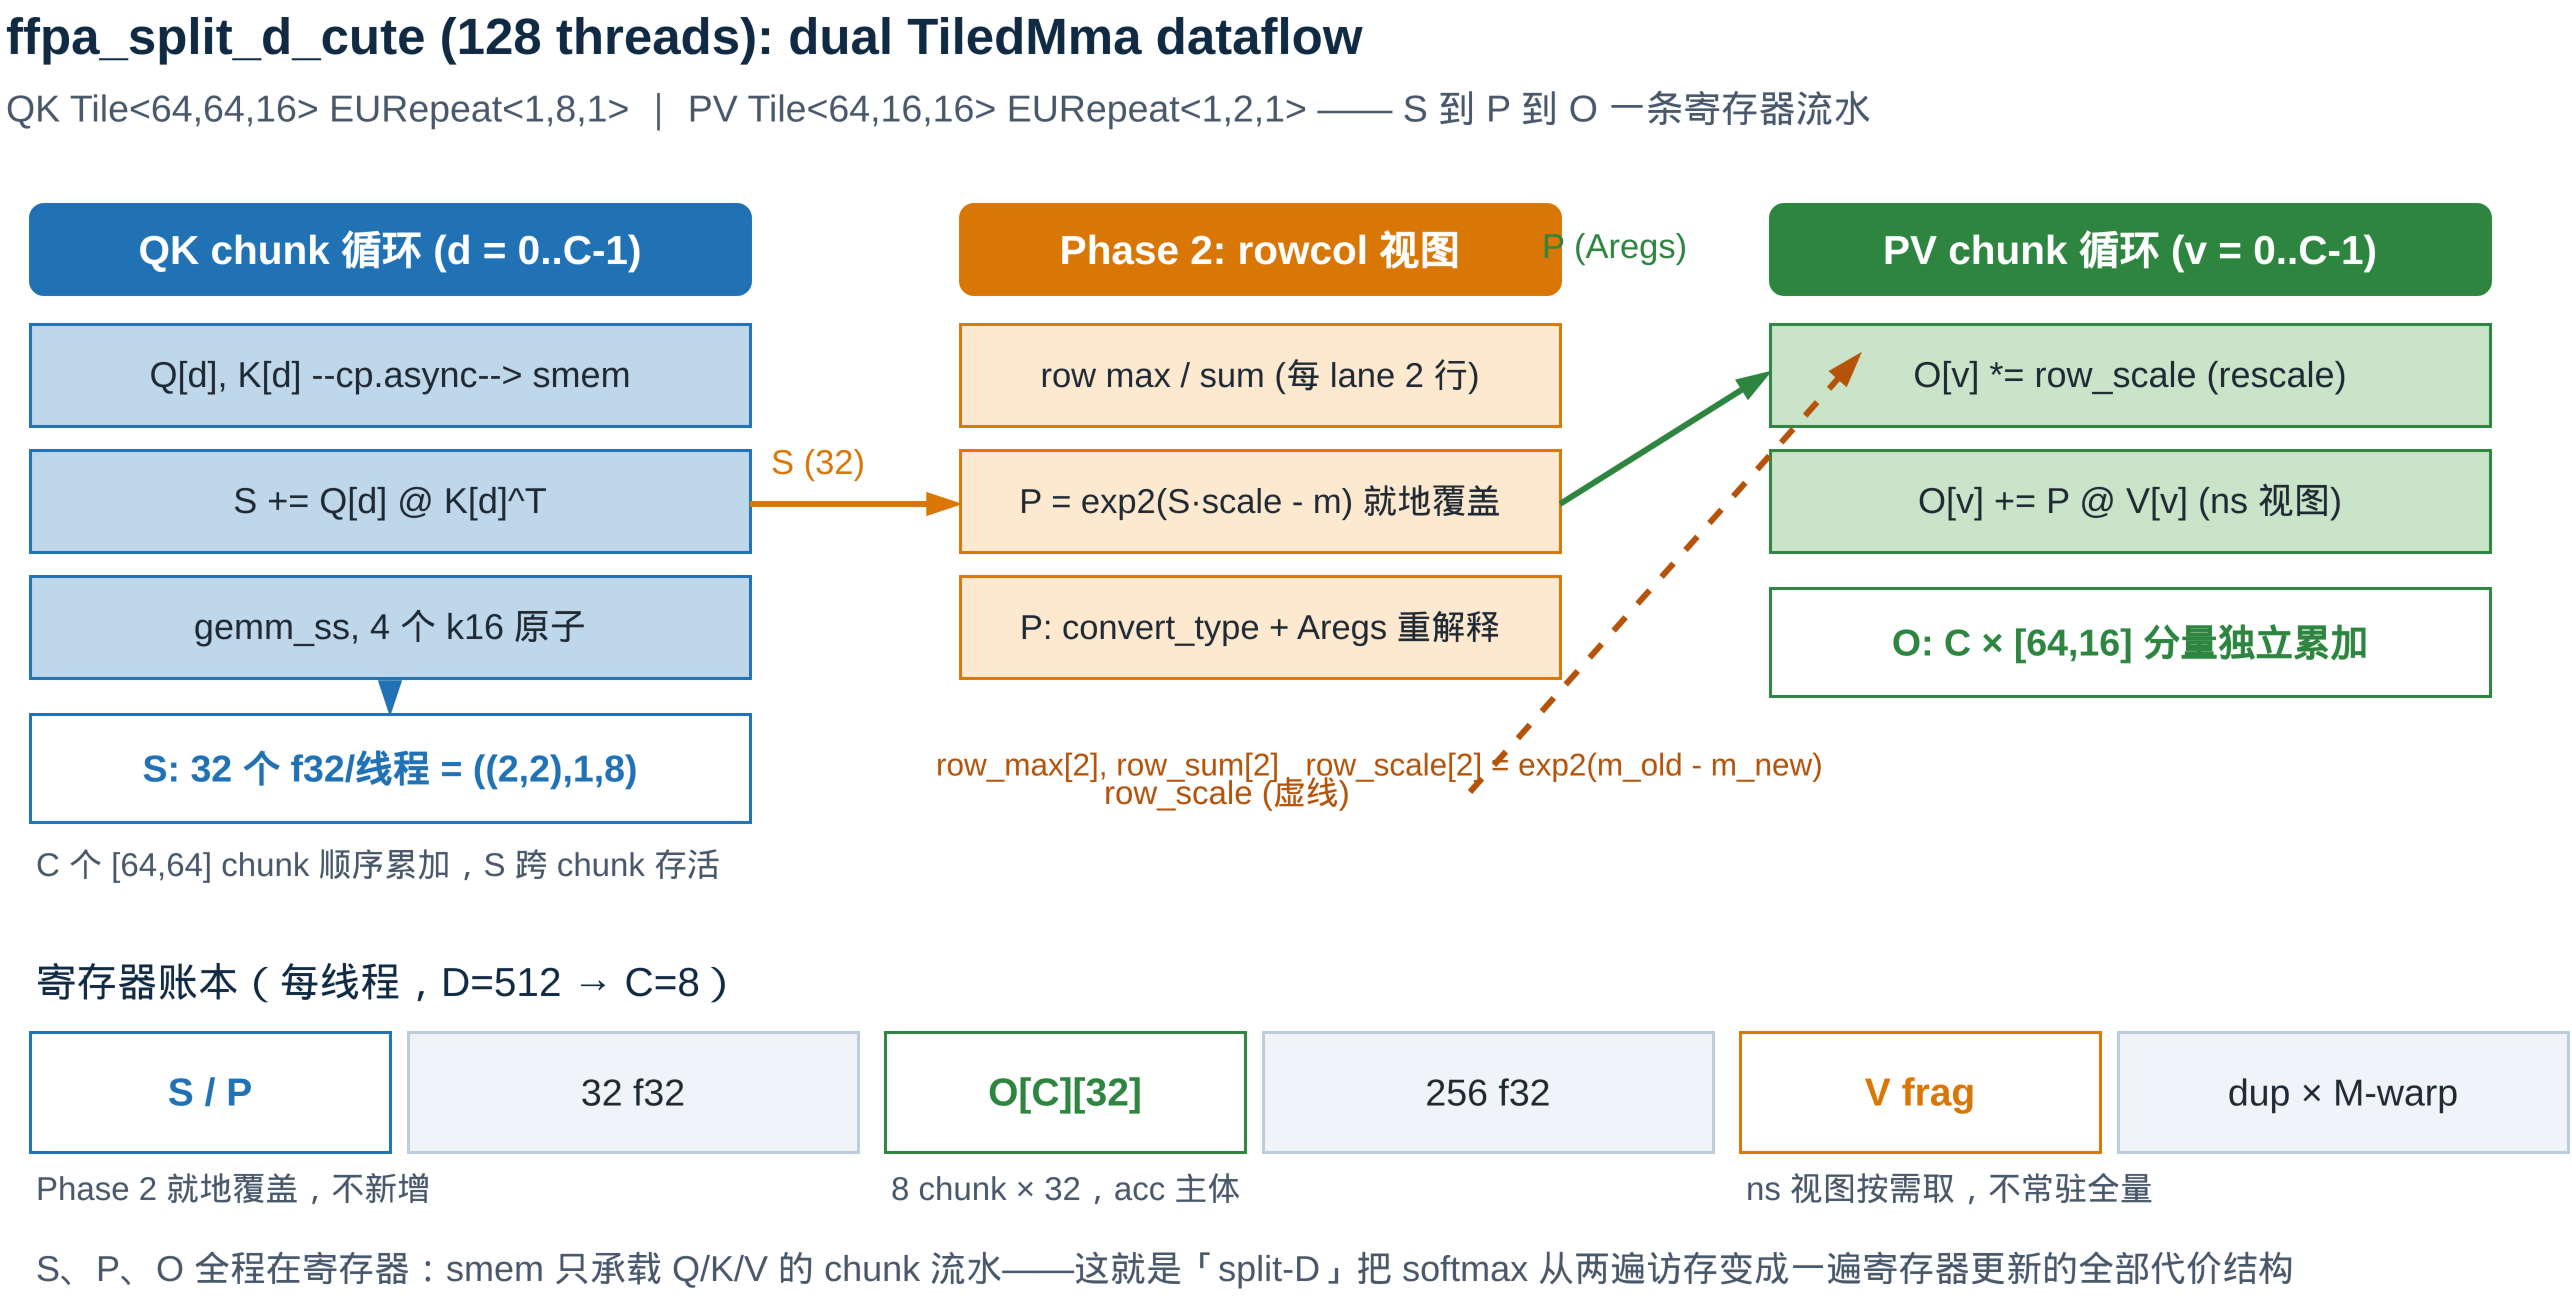
\includegraphics[width=0.92\textwidth]{figures/drawio/fig-26-1-dual-mma/fig-26-1.png}
\begin{tikzpicture}[font=\tiny, >=Stealth,
  hb/.style={align=center, inner sep=2pt, font=\bfseries\fontsize{4.6}{5.2}\selectfont},
  bx/.style={align=center, inner sep=2pt, font=\fontsize{4.2}{4.8}\selectfont},
  tx/.style={align=left, inner sep=1pt, font=\fontsize{4.2}{4.8}\selectfont, anchor=west},
]
  % 左栏：QK chunk 循环（S 累加器跨 chunk 存活）
  \node[hb, fill=tkBlue, text=white, text width=4.20cm] at (2.10,-0.12)
    {QK chunk 循环（$d = 0..C{-}1$）};
  \node[bx, draw=tkBlue, fill=tkFillBlue, text width=3.90cm] at (2.10,-0.75)
    {Q[$d$], K[$d$] $\xrightarrow{\texttt{cp.async}}$ smem};
  \node[bx, draw=tkBlue, fill=tkFillBlue, text width=3.90cm] at (2.10,-1.51)
    {S $+=$ Q[$d$] @ K[$d$]$^{\top}$};
  \node[bx, draw=tkBlue, fill=tkFillBlue, text width=3.90cm] at (2.10,-2.27)
    {gemm\_ss，4 个 k16 原子};
  \node[bx, draw=tkBlue, fill=white, text=tkBlue, text width=3.90cm,
    font=\bfseries\fontsize{4.2}{4.8}\selectfont] at (2.10,-3.03)
    {S：32 个 f32/线程 $=$ ((2,2),1,8)};
  \node[tx, text width=4.20cm] at (0,-3.55)
    {C 个 [64,64] chunk 顺序累加，S 跨 chunk 存活};
  % 中栏：Phase 2（rowcol 视图上的 softmax）
  \node[hb, fill=tkOrange, text=white, text width=3.60cm] at (6.90,-0.12)
    {Phase 2：rowcol 视图};
  \node[bx, draw=tkOrange, fill=tkFillOrange, text width=3.30cm] at (6.90,-0.75)
    {row max / sum（每 lane 2 行）};
  \node[bx, draw=tkOrange, fill=tkFillOrange, text width=3.30cm] at (6.90,-1.51)
    {scores $=$ exp2(S$\cdot$scale $-$ m) 写回 S};
  \node[bx, draw=tkOrange, fill=tkFillOrange, text width=3.30cm] at (6.90,-2.27)
    {P：convert\_type $+$ Aregs 重解释};
  \node[bx, text=tkOrange!80!black, text width=4.30cm] at (6.90,-3.05)
    {row\_max[2], row\_sum[2]\\row\_scale[2] $=$ exp2($m_{\mathrm{old}} - m_{\mathrm{new}}$)};
  % 右栏：PV chunk 循环（O 分量独立 rescale 与累加）
  \node[hb, fill=tkGreen, text=white, text width=4.20cm] at (12.30,-0.12)
    {PV chunk 循环（$v = 0..C{-}1$）};
  \node[bx, draw=tkGreen, fill=tkFillGreen, text width=3.90cm] at (12.30,-0.75)
    {O[$v$] $*=$ row\_scale（rescale）};
  \node[bx, draw=tkGreen, fill=tkFillGreen, text width=3.90cm] at (12.30,-1.51)
    {O[$v$] $+=$ P @ V[$v$]（ns 视图）};
  \node[bx, draw=tkGreen, fill=white, text=tkGreen, text width=3.90cm,
    font=\bfseries\fontsize{4.2}{4.8}\selectfont] at (12.30,-2.27)
    {O：$C \times$ [64,64] 分量独立累加（每块 4 个 N-tile）};
  % 主数据流箭头：S -> Phase 2 -> P -> PV
  \draw[->, tkOrange, semithick] (4.28,-1.45) -- (5.02,-1.45);
  \node[tx, text=tkOrange] at (4.35,-1.28) {S (32)};
  \draw[->, tkGreen, semithick] (8.78,-1.45) -- (10.18,-1.45);
  \node[tx, text=tkGreen] at (8.85,-1.28) {P (Aregs)};
  % row_scale 虚线耦合：Phase 2 尾部 -> PV 的 rescale 框
  \draw[->, dashed, tkOrange!80!black, semithick]
    (7.90,-3.42) -- (10.18,-3.42) -- (10.18,-2.42) -- (10.28,-2.42);
  \node[align=center, inner sep=1pt, font=\fontsize{4.2}{4.8}\selectfont,
    text=tkOrange!80!black] at (9.30,-3.68) {row\_scale（虚线）};
  % 底部：寄存器占用
  \node[font=\bfseries\fontsize{4.6}{5.2}\selectfont, anchor=west] at (0,-4.10)
    {寄存器占用（每线程，$D=512 \to C=8$）};
  \node[bx, draw=tkBlue, fill=white, text=tkBlue, text width=1.30cm,
    font=\bfseries\fontsize{4.2}{4.8}\selectfont] at (0.75,-4.55) {S $\to$ P};
  \node[bx, draw=gray!60, fill=gray!12, text width=2.10cm] at (2.90,-4.55) {32 f32 / 32 f16};
  \node[tx, text width=4.2cm] at (0,-4.92) {softmax 写回 S；convert\_type 生成新 P fragment};
  \node[bx, draw=tkGreen, fill=white, text=tkGreen, text width=1.30cm,
    font=\bfseries\fontsize{4.2}{4.8}\selectfont] at (5.95,-4.55) {O[$C$][32]};
  \node[bx, draw=gray!60, fill=gray!12, text width=2.10cm] at (8.10,-4.55) {256 f32 逻辑值（spill）};
  \node[tx] at (5.20,-4.92) {8$\times$32，已超 255 寄存器上限};
  \node[bx, draw=tkOrange, fill=white, text=tkOrange!80!black, text width=1.30cm,
    font=\bfseries\fontsize{4.2}{4.8}\selectfont] at (11.15,-4.55) {V frag};
  \node[bx, draw=gray!60, fill=gray!12, text width=2.10cm] at (13.30,-4.55) {每 M-warp 各一份};
  \node[tx] at (10.40,-4.92) {每线程私有，跨 warp 重复};
  \node[tx, text width=15.0cm] at (0,-5.35)
    {S/P 的更新在寄存器路径，O 的 256 个逻辑值超过 255 上限会 spill；smem 只承载 Q/K/V 的 chunk 流水——
     这就是\textbf{split-D}把 softmax 从两遍访存变成一遍寄存器更新的代价所在};
\end{tikzpicture}
\caption{双 TiledMma 的数据流：QK 沿 $D$ 累加成 $S$（32 个 f32 寄存器跨
chunk 存活），softmax 写回 $S$，再由 \texttt{convert\_type} 产生 f16 $P$，
Aregs 重解释其布局后交给 PV；$O$ 的每个 chunk 分量独立 rescale 与累加，
\texttt{row\_scale}（虚线）耦合两个循环。底部为寄存器占用：$S$ 为 32 个
f32、$P$ 为新生成的 32 个 f16 逻辑值；$O[C][32]$ 共 256 个 f32 逻辑值
（$C{=}8$，已超过 255 个寄存器的硬上限，会 spill）、V fragment 在每个
M-warp 中各有一份私有副本——smem 只承载 Q/K/V 的 chunk 流水。}
\label{fig:26-1}
\end{figure}

\section{性能分析}

本章不给新的实测数字，原因与第~\ref{ch:25}~章相同：本机没有复测 FFPA 的
完整 bench（第~\ref{ch:19}~章给出其性能数据与口径）。这里只做两件事：转录
源码注释里的既有声明（注明出处），并从本章的类型视角讨论 Split-D 抽象层的
运行时成本结构。

源码头注释（\texttt{ffpa\_\allowbreak{}attn.\allowbreak{}cuh} L16--17）的性能声明是：

\begin{quote}
  \textit{性能 (B=1,H=32,N=8192,D=512, SM120a RTX PRO 5000):
  cuDNN SDPA: 57.2 TFLOPS | FFPA TMA WS: 110.7 TFLOPS (1.94x)}
\end{quote}

读数时注意三点口径。（1）这是 TMA + WS 版（256 线程、双角色）的数字，不是
本章精读的 cp.async 版。（2）设备标称 SM120a RTX PRO 5000，而本仓库 README 的
同类标称常写 RTX 5090，同一 sm120 家族的两种卡，绝对值不可直接互比
（第~\ref{ch:19}~章的核对与 CHECKLOG 记录同此）。（3）1.94x 是相对 cuDNN SDPA
的加速比，比较对象与精度配置（f16 输入、f32 累加）需与 bench 脚本核对后才可
引用。

从类型视角看，Split-D 的抽象开销可以逐项归零：

\begin{itemize}[itemsep=2pt,topsep=2pt]
  \item \texttt{kDChunks}、\texttt{k\allowbreak{}QChunk\allowbreak{}Elements} 等全是
        \texttt{constexpr}，chunk 循环的步长、stage 偏移、池大小都在编译期
        折叠成立即数，运行时（在开启优化后）与手写版本无差别。
  \item \texttt{local\_tile}/\texttt{partition\_*} 的坐标算术全部由模板
        推导，编译产物里剩下的是少数 \texttt{mad} 与常量偏移。
  \item 实际的运行时成本在算法侧（chunk 循环的额外 barrier、V 的重复加载），
        与用不用 CuTe 无关。第~\ref{ch:19}~章对这两项开销的量化结论是
        \textbf{Stage 上限压到 2--3，同步开销主导}。
\end{itemize}

CuTe 在 Split-D 上的收益与代价都不在运行时，而在类型可断言：本章测试
（26.9 节）能在不启动 kernel 的情况下核对双 TiledMma 的每条推导。

\section{常见坑}

\textbf{坑一：推 V 的 fragment 布局必须去掉 swizzle。}
\texttt{partition\_\allowbreak{}fragment\_\allowbreak{}B} 要的是值的线程归属，而 swizzle 只改变
元素的 smem 地址。直接用带 SW128 的 \texttt{Smem\allowbreak{}Layout\allowbreak{}Vt} 去推，XOR
置换会混进逻辑坐标，fragment 布局与真值错位：正确做法是
\texttt{get\_\allowbreak{}nonswizzle\_\allowbreak{}portion} 之后再推（L137--141）。但 S2R 的
smem 地址仍由 \texttt{s2r\_thr\_v.partition\_S(sVt\_stg)} 用带 swizzle 的 storage
视图计算，两份视图职责不同。

\textbf{坑二：\texttt{convert\_\allowbreak{}type} 与 \texttt{Aregs} 的区别。}
当前源码先做类型转换、再做布局重解释（L301--303）。但
\texttt{NumericArrayConverter} 只看底层平坦数组，不按 layout 的连续段
分组；Aregs 只换索引。不能用“反序会转换错误分组”解释这段顺序，也不能
把 f32$\to$f16 的转换称为原寄存器零拷贝。

\textbf{坑三：\texttt{o\_\allowbreak{}acc\_\allowbreak{}storage} 的初始化在 chunk 循环外、只做一次。}
它在每个 kv\_tile 迭代里都是\emph{累加}目标，清零只在 kernel 开头
（L174--176）。若把它挪进 kv\_tile 循环，$O$ 会丢失历史。

\textbf{坑四：\texttt{v\_write\_pv} 的初值必须与 Phase 0 的预取数对接。}
Phase 0 写了 $\mathrm{Sv}-1$ 个 chunk，PV 循环从槽位号
$(\mathrm{Sv}-1)\bmod \mathrm{Sv}$ 继续（L308）。改 Phase 0 的预取个数
而忘了这里，会写坏正在被读的 chunk。

\textbf{坑五：chunk 循环里的 \texttt{\_\allowbreak{}\_\allowbreak{}syncthreads\allowbreak{}()} 属于槽位复用协议。}
QK 每轮末尾（L269）与 PV 每轮末尾（L350）的同步不是可有可无的：它们保证本轮
读过的 smem 槽位在下一轮被覆写之前所有线程都已读完；删掉它，表现是
高频偶发数值错误，且随 stage 数增大而加剧。

\textbf{坑六：行状态只有 2 个，但列有 16 个：shfl 掩码只到 2。}
\texttt{row\_max}/\texttt{row\_sum} 的长度是 \texttt{kORows}$=2$，
行内归约靠 \texttt{\_\allowbreak{}\_\allowbreak{}shfl\_\allowbreak{}xor\_\allowbreak{}sync} 的掩码 1 与 2（4 个 lane 一组，
L281--282 与 L291--292）。多加一层掩码 4 会把\emph{另一个 warp 段}的行
卷进来（warp 内 8 个 lane 组对应 8 个不同行块），数值立刻错。

\textbf{坑七：chunk 宽度、smem 池、TMA box 三者必须同步改。}
把 \texttt{kDChunk} 从 64 改成别的值时，SW128 原子、TMA box
（\texttt{Shape\allowbreak{}<\_\allowbreak{}64,\allowbreak{}\_\allowbreak{}64>}）、\texttt{kDChunks} 与 V 的 fragment 预计算
全部要跟着动，一个 64 改三处是这一族 kernel 改动时的固定代价。

\section{面试要点速查}

\begin{enumerate}[itemsep=3pt,topsep=3pt]
  \item \textbf{为什么 QK 的 TiledMma 要 Tile$\langle64,64,16\rangle$，
        而 PV 只要 $\langle64,16,16\rangle$？}
        QK 的 N 向 EURepeat 变成 8，一次覆盖 $S[64,64]$，省掉 N-tile
        循环（提升计算密度）；PV 的单次调用视图是 $[64,16]$，完整 O chunk
        则由 4 个 N-tile 组成 $[64,64]$，外层 V-chunk 再遍历其它 chunk。
        小 tile 控制单次调用的寄存器视图；两者的完整 C fragment 大小相同
        （$32$），因为完整输出形状与线程数相同。
  \item \textbf{Split-D 不改变 fragment 形状是什么意思？}
        $S$ 的 fragment 在 chunk 循环前后都是 $((2,2),1,8)=32$ 个 f32；
        chunk 循环表达的是同一个数组跨迭代累加。变的只是循环结构与
        归约树。
  \item \textbf{$S$ 怎么变成 $P$？为什么不需要 shuffle/smem？}
        先由 \texttt{convert\_type} 做 f32$\to$f16 数值转换并产生新 fragment；
        \texttt{convert\_\allowbreak{}layout\_\allowbreak{}acc\_\allowbreak{}Aregs} 再按 $m16n8$ 的 C 与
        $m16k16$ 的 A 映射重解释布局（C 的列向 2 值 $=$ A 的 K 向 2 值）。
        免掉的是 smem 往返，Aregs 本身仍是不搬数据的布局重解释。SM80
        $k8$ atom 的 A/C 布局相同，可拆两次 PV 继续复用；其他约定要重推。
  \item \textbf{为什么 V 的 fragment 布局要预先算、且用 nonswizzle 版本？}
        循环里只换指针不改布局——算一次省每轮推导；去掉 swizzle 是因为
        它只改地址不改值的线程归属。S2R 的 smem 地址另由
        \texttt{partition\_S} 在带 swizzle 的视图上计算。
  \item \textbf{每个线程持有多少 $O$ 逻辑累加值？}
        $C\times32$ 个 f32 \emph{逻辑累加值}：$D=512$ 时 256 个，已超过
        每线程 255 个寄存器的硬上限，实际需要 spill。第一维来自 chunk
        循环（问题尺寸），第二维来自 fragment 布局（TiledMma）。
  \item \textbf{行归约为什么要用到 \texttt{shfl\_xor} 掩码 1 和 2？}
        $m16n8$ 的 C fragment 里一行由 4 个 lane 拼成（每 lane 2 行 $\times$
        16 列），掩码 1 与 2 恰好把 4 个 lane 的两两组合并；再多就跨行块了。
  \item \textbf{smem 池的偏移为什么用指针算术而不是 layout 的 stage 维？}
        当前实现选择指针算术，不是 CuTe 的必然要求。真实的 stage mode
        应使用 stride 等于一块 chunk 元素数的非零 stride；只有 stride-0
        伪维才表示所有 stage 落到同一元素，从而使 \texttt{cosize} 与
        partition 不再对应池大小。
  \item \textbf{chunk 数与 stage 数是什么关系？}
        正交：chunk 数是问题尺寸（head\_dim/64），stage 数是流水深度
        （smem 预算）。两者的相位关系与约束见第~\ref{ch:19}~章。
\end{enumerate}

\section{最小测试与动手实验}

本章测试（\texttt{tests/\allowbreak{}ch26\_\allowbreak{}ffpa\_\allowbreak{}cute.\allowbreak{}cu}）与前几章的不同之处是
以 host 端类型断言为主：这部分不启动 kernel，只对 traits 与 fragment
做静态/运行时断言，全部来自 26.3 节的代数。下文先列这部分输出，再列 device
probe 与小规模 kernel case：

\begin{enumerate}[itemsep=2pt,topsep=2pt]
  \item \textbf{D-chunk 常量}：对 $D\in\{64,128,192,512\}$ 断言
        \texttt{kDChunks}$=D/64$ 与两个 chunk 池
        $\mathrm{cosize}=64\times64$；
  \item \textbf{双 TiledMma 推导链}：QK 的 \texttt{tile\_\allowbreak{}size\_\allowbreak{}mnk}
        $=(64,64,16)$、PV $=(64,16,16)$，线程数均为 128；
  \item \textbf{fragment 恒等式}：两个
        \texttt{partition\_\allowbreak{}fragment\_\allowbreak{}C}$((64,64))$ 的每线程元素数都是 32。
        rowcol 后的行列数 $(2,16)$；Aregs 重解释前后元素数守恒；
  \item \textbf{switch 语义}：\texttt{local\_tile} 在 $(64,64)$ tile 与
        $(row\_tile, d\_chunk)$ 坐标下的首元素地址等于
        \texttt{row\_\allowbreak{}tile*64*D + d\_\allowbreak{}chunk*64}。
\end{enumerate}

再加两个小规模 kernel 正确性 case（与第~\ref{ch:19}~章的覆盖互不重复）：

\begin{itemize}[itemsep=2pt,topsep=2pt]
  \item case E：$D=192$（3 个 chunk，且与 $\mathrm{Sk}{=}3$ 相等，用来测
        chunk 数 $=$ stage 数的边界；实际预取深度为 $\mathrm{Sk}-1=2$）、$N=128$、$H=2$、
        $\mathrm{Sk}{=}3,\mathrm{Sv}{=}2$；
  \item case F：$D=128$（2 个 chunk，$\mathrm{Sk}{=}2$）、$N=128$、$H=2$。
\end{itemize}

两者都与 CPU fp64 参考对照（容差 \texttt{TOL\_F16ACC}），运行：

\begin{lstlisting}[style=console]
cd book/tests && CUDA_VISIBLE_DEVICES=6 ./build_tests.sh --arch sm_120a --ch ch26
\end{lstlisting}

本机实测输出（sm\_120a，6 号卡）：

{\scriptsize
\begin{lstlisting}[style=console]
PASS case A chunk constants D=64 (kDChunks=1): mismatches=0 (4 checks)
PASS case A chunk constants D=128 (kDChunks=2): mismatches=0 (6 checks)
PASS case A chunk constants D=192 (kDChunks=3): mismatches=0 (8 checks)
PASS case A chunk constants D=512 (kDChunks=8): mismatches=0 (18 checks)
PASS case B dual TiledMma derivation chain (D=512): mismatches=0 (6 checks)
probe: rowcol=(2,16) aregs_elems=32
PASS case B2 device probe: rowcol (2,16) & Aregs 32 elems: mismatches=0 (3 checks)
PASS ffpa split-d cute D=192 N=128 Sk=3 Sv=2 B=1 H=2: max_abs_err=8.481e-05 (tol=5.0e-02)
PASS ffpa split-d cute D=128 N=128 Sk=2 Sv=2 B=1 H=2: max_abs_err=8.084e-05 (tol=5.0e-02)
ALL OK
\end{lstlisting}
}

\section*{延伸阅读}

\begin{itemize}[itemsep=2pt,topsep=2pt]
  \item @竹熙佳处《写给大家看的 CuTe 教程：Layout Compose \& Inverse》——
        $S\to P$ 布局变换的完整讲法（Tri Dao 的几何法与 @reed 的代数法），
        本章 26.3.3 节与第~\ref{ch:25}~章 25.3.4 节的主参考。\\
        \url{https://zhuanlan.zhihu.com/p/1962625273636845008}
  \item @reed《cute 之 高效 GEMM 实现》——TiledMMA 的组装层次、
        多级流水的写法与 Epilogue 的 smem 中转；同系列《cute 之 简单
        GEMM 实现》给出最小版本的组装范式，配合 26.3.1 的推导链与
        26.4 的相位阅读一起看。\\
        \url{https://zhuanlan.zhihu.com/p/675308830}
  \item @竹熙佳处《写给大家看的 CuTe 教程：tiled mma》——fragment 视角的
        线程-值映射，26.3.2 节两个恒等式的入门读物。\\
        \url{https://zhuanlan.zhihu.com/p/1937145378446226159}
  \item @DefTruth《FFPA(Split-D)：FA2 无限 HeadDim 扩展》——
        本主题在中文社区最系统的公开文章，Split-D 的动机与 RD 波形分析
        可与第~\ref{ch:19}~章的推导对读。\\
        \url{https://zhuanlan.zhihu.com/p/13975660308}
  \item @DefTruth《图解：从 Online-Softmax 到 FlashAttention V1/V2/V3》——
        online softmax 的图解（本书第~\ref{ch:15}~章的主参考），
        配合本章 26.3.2 的 rowcol 代数读更佳。\\
        \url{https://zhuanlan.zhihu.com/p/668888063}
  \item @66RING《使用 cutlass cute 复现 flash attention》——CuTe 版 FA 的
        工程化复现，可与第~\ref{ch:25}~章的四个实现对照。\\
        \url{https://zhuanlan.zhihu.com/p/696323042}
  \item @DeclK《CUTLASS CUTE 系列（1--5）》——布局代数与 MMA/COPY 抽象的
        系统性替代读物，作为第~\ref{ch:20}--\ref{ch:22}~章的复习材料。\\
        \url{https://zhuanlan.zhihu.com/p/1983922984805742098}
\end{itemize}

% ch26b-cute-persist-d-flash-attn.tex — CuTe 应用（四）：sm_120 持久化 FlashAttention
% ——超越 cuDNN（2026-09-22，源码 flash_attn.cuh Phase 8，L3490-4177）
% 图：全 TikZ（用户指定）；代码段引用 ../flash_attn.cuh linerange。
\chapter{CuTe 应用（四）：SM120 持久化 FlashAttention——超越 cuDNN}\label{ch:26b}

\section{本章导读}

第~\ref{ch:25}~章结束时，我们已经拿到三个 CuTe 版 FlashAttention：cp.async 统一流水、
TMA + 单 consumer warp specialization、FA3 式双 consumer。它们回答的都是布局
事实搬进类型之后 attention 长什么样，但性能口径上还缺一个对照：这些教学实现离
厂商库到底有多远？本章把三个实现里各自最强的部分拼起来，再补上两个只有在
kernel 全权可控时才做得出的优化（softmax scale$\cdot\log_2 e$ 融合、
persistent CTA），得到
\texttt{flash\_\allowbreak{}attn\_\allowbreak{}cute\_\allowbreak{}persist\_\allowbreak{}d\_\allowbreak{}sm120}
（flash\_attn.cuh L3635，\texttt{NOTES\_\allowbreak{}V2\_\allowbreak{}ENABLE\_\allowbreak{}CUTE}
宏块 Phase~8）：在 RTX PRO 5000（sm\_120，110 SM）上
$H{=}32$/$N{=}8192$/$D{=}128$ dense 场景实测 240.1 TFLOPS，为 cuDNN SDPA
（230.2 TFLOPS）的 1.04 倍。这是全书第一个在绝对性能上越过厂商库的
attention kernel。

本章的四条主线，都指向超越 cuDNN：

\begin{itemize}[itemsep=1pt,topsep=2pt]
  \item \textbf{WS 双角色}（\S\ref{sec:26b-arch}）：128 线程 producer（只发 TMA）+
        256 线程 consumer（只做 MMA），\texttt{setmaxnreg} 把 producer 的寄存器
        划给 consumer，这是 sm\_120 上把搬运与计算物理解耦的唯一手段；
  \item \textbf{Q 寄存器持久化}（\S\ref{sec:26b-persistq}）：Q tile 对整个 KV 循环
        不变，smem$\to$寄存器只搬一次，之后每次 $QK^\top$ 都是 A-operand 常驻的
        \texttt{gemm\_rs}；
  \item \textbf{softmax scale 融合}（\S\ref{sec:26b-scale-math}）：把
        $s=\text{scale}\cdot\log_2 e$ 一次性乘进 Q fragment，softmax 的 max/exp
        两个循环里的逐元素乘法全部消失；
  \item \textbf{persistent CTA}（\S\ref{sec:26b-persistent}）：dense 场景 grid
        收缩到 SM 数，每个 CTA 串行处理多个 q-tile，消除 wave 量化尾损。
\end{itemize}

\textbf{前置章节}：第~\ref{ch:15}--\ref{ch:16}~章（attention 数学与 FA2 online
softmax）、第~\ref{ch:17}~章（TMA 与 mbarrier 协议）、第~\ref{ch:21}--\ref{ch:22}~章
（TiledCopy 与 TiledMMA）、第~\ref{ch:25}~章（CuTe FA 三实现对照：本章直接复用其
五个工具函数）。\textbf{源码区间}：flash\_attn.cuh L3490--4177（Phase 8 宏块）。
\textbf{编译宏与架构}：\texttt{NOTES\_\allowbreak{}V2\_\allowbreak{}ENABLE\_\allowbreak{}CUTE}，
编译目标 \texttt{sm\_120a} 与 \texttt{sm\_120f} 均可：\texttt{setmaxnreg} 的实际
生效条件是 TMA 目的地址用 \texttt{shared::cta}，且 \texttt{\_\_launch\_\allowbreak{}bounds\_\allowbreak{}(384,~1)}
写双参数，与 arch 后缀无关（完整决策树见 \S\ref{sec:26b-setmaxnreg}）。本章 kernel
只依赖 sm\_80 级的 mma.sync 与 sm\_90 级的 TMA/mbarrier，任何 Blackwell（sm\_120）
显卡均可运行。

\section{问题与动机：为什么专用 kernel 能赢厂商库}\label{sec:26b-motivation}

手写 kernel 赢 cuDNN 在 Hopper（sm\_90）时代几乎不可信：cuDNN 在 H100 上用
WGMMA + warp specialization + TMEM 调到了接近理论峰值，普通开发者用 CuTe 从零追赶
成本极高。但 sm\_120（Blackwell 消费线/专业线）不一样：这块芯片没有
WGMMA（sm\_90 专属）、没有 tcgen05/TMEM（sm\_100 专属），cuDNN 与我们一样，
只剩同一条张量核路径：

\begin{equation*}
  \text{mma.sync.aligned.m16n8k16.row.col.f32.f16.f16.f32}
\end{equation*}

于是在 sm\_120 上，厂商库与手写的差距不再是指令代差，而全部落在协议设计
上：tile 几何、流水深度、寄存器分配、softmax 的指令数、wave 尾损。实测基线
（PRO 5000，$B{=}1$/$H{=}32$/$N{=}8192$/$D{=}128$ fp16，dense）：

\begin{center}
\begin{tabular}{lcc}
\toprule
实现 & TFLOPS & 相对 cuDNN \\
\midrule
cuDNN SDPA（\texttt{CUDNN\_ATTENTION} 后端） & 230.2 & 1.00$\times$ \\
本章 kernel & \textbf{240.1} & \textbf{1.04$\times$} \\
\bottomrule
\end{tabular}
\end{center}

领先的来源逐项拆解如下（A/B 实测，独立 kernel 上各开关单独计量）：
\texttt{exp2f} 替代 \texttt{expf}（\texttt{-{}-use\_\allowbreak{}fast\_\allowbreak{}math}，
+2\%\textasciitilde4\%）、softmax scale 融合（+3\%\textasciitilde4\%）、persistent CTA
（dense 中等序列 +2\%\textasciitilde6\%）、FA-4 条件重缩放（长序列收益，复用
第~\ref{ch:16}~章结论）。四项都是把协议里的一次浪费换成零开销，没有一项依赖复杂技巧。

还有一个工程动机：厂商库的 SDPA 对\textbf{非标准形状}（GQA 折叠、滑窗 causal、
head\_dim=96 这类非 2 的幂）经常落入慢速 fallback；专用 kernel 按自己的 tile 几何
原生支持这些形状。

\section{数学原理}\label{sec:26b-math}

\subsection{log2 域 online softmax 回顾}

第~\ref{ch:15}--\ref{ch:16}~章已经推导过 online softmax，这里只保留本章需要的形态。
对每个 KV tile，softmax 的在线更新为
\begin{align}
  m^{(t)} &= \max\!\big(m^{(t-1)},\ \max_j s_j^{(t)}\big), \label{eq:26b-max}\\
  \ell^{(t)} &= \ell^{(t-1)} e^{m^{(t-1)}-m^{(t)}} + \sum_j e^{s_j^{(t)}-m^{(t)}}, \label{eq:26b-sum}\\
  O^{(t)} &= O^{(t-1)} e^{m^{(t-1)}-m^{(t)}} + \sum_j e^{s_j^{(t)}-m^{(t)}} v_j^{(t)}, \label{eq:26b-o}
\end{align}
其中 $s_j = \text{scale}\cdot q\cdot k_j$。GPU 上把 $e^x$ 换成
$\mathrm{exp2}(x\cdot\log_2 e)$（一条 \texttt{MUFU.EX2} 即可），为此把
$\log_2 e$ 预乘进 scale：
\begin{equation}\label{eq:26b-log2domain}
  s_j^{\log_2} = \underbrace{\text{scale}\cdot\log_2 e}_{s}\cdot (q\cdot k_j),
  \qquad e^{s_j - m} = \mathrm{exp2}\!\big(s_j^{\log_2} - m^{\log_2}\big).
\end{equation}
此后所有 max/sum/rescale 都在 log2 域完成，epilogue 再乘回 $\ln 2$（若需要 lse）。

\subsection{FA-4 条件重缩放}

式~\eqref{eq:26b-sum}/\eqref{eq:26b-o} 里的 $e^{m^{(t-1)}-m^{(t)}}$ 要求每个 tile
都对 $\ell$ 和 $O$ 做一次逐元素乘法。FA-4 的观察是：随机数据下新 tile 的 max 很少
超过历史 max 太多。记 $\Delta = m^{(t-1)} - m^{(t)} \le 0$（log2 域），当
\begin{equation}\label{eq:26b-fa4}
  \Delta \ge -\tau, \qquad \tau = 8 = \log_2 256
\end{equation}
时，$2^{\Delta}$ 只会让 P 累计最多膨胀 $256\times$：fp16 的 P 最大 65504，
f32 累加器余量更大，因此可以跳过这次重缩放：$m$ 保持旧值
（stale max）、$O$/$\ell$ 原样累加。膨胀的部分在 epilogue 的 $1/\ell$ 里全部
抵消（分子分母同乘一个常数）。dense 数据下命中率高（实测 95\%+ 的 tile 满足
\eqref{eq:26b-fa4}），只有新 tile 的 max 明显更大时才付出重缩放代价。第~\ref{ch:16}~章
的手写版已经给过这个结论，本章把它原样搬进 CuTe 版
（\texttt{online\_\allowbreak{}safe\_\allowbreak{}softmax\_\allowbreak{}fa4}，
flash\_attn.cuh L3587）。

\subsection{softmax scale$\cdot\log_2 e$ 融合}\label{sec:26b-scale-math}

式~\eqref{eq:26b-log2domain} 里，$\log_2 e$ 折进 scale 只是提前一次乘法，
每个 score 元素仍然要乘 $s$ 两次：max pass 一次（\eqref{eq:26b-max}）、
exp pass 一次（\eqref{eq:26b-sum}）。对一个 $128\times 64$ 的 S tile，这是
$2\times 128\times 64 / 256\text{thread} = 64$ 次 FMUL/线程/tile，
而 QK GEMM 本身（m16n8k16 路径）每 tile 每线程只有 64 条 HMMA：softmax 的
scale 乘法指令数与 tensor core 指令数同量级，是纯浪费。

本章的优化是把 $s$ 从乘在 S 上改为乘在 Q 上：
\begin{equation}\label{eq:26b-fold}
  S_{\text{fused}} = (s\odot Q)\,K^\top = s\cdot(QK^\top) = s\cdot S_{\text{raw}},
\end{equation}
其中 $\odot$ 是逐元素乘。等价性来自两条初等性质（$s>0$）：
\begin{align}
  \max_j (s\cdot x_j) &= s\cdot \max_j x_j, \label{eq:26b-maxcommute}\\
  \mathrm{exp2}(s\cdot x - m) &= \mathrm{exp2}(S_{\text{fused},j} - m). \label{eq:26b-expcommute}
\end{align}
Q fragment 在寄存器里、对整个 KV 循环不变（persist-D），所以
\eqref{eq:26b-fold} 的代价只是 \texttt{size(tCrQ)} 次一次性 FMUL（Q s2r 后立即做），
外加 $s\odot Q$ 引入一次 fp16 重舍入。收益是 softmax 两个 pass 的逐元素乘法
归零。这条优化的前提是 persist-D：如果 Q 每个 tile 重新装载
（split-Q/FA3 布局），折叠本身也要每 tile 做一次，收益减半。

\begin{figure}[H]
\centering
\begin{tikzpicture}[
  font=\footnotesize,
  every node/.append style={align=center},
  box/.style={draw=tkBlue, fill=tkFillBlue, rounded corners=1.5pt, minimum height=0.7cm, inner sep=3pt},
  ops/.style={draw=tkPurple, fill=white, rounded corners=1.5pt, minimum height=0.7cm, inner sep=3pt},
  mul/.style={draw=tkOrange, fill=white, rounded corners=1.5pt, minimum height=0.6cm, inner sep=2pt, font=\scriptsize},
  arr/.style={-{Stealth[length=2.2mm]}, thick},
]
% before path
\begin{scope}
  \node[box] (q1) at (0,0) {$Q$};
  \node[box, right=0.5 of q1] (k1) {$K^\top$};
  \node[ops, right=0.5 of k1] (qk1) {$QK^\top$\\{\scriptsize HMMA}};
  \node[mul, right=0.35 of qk1] (m1a) {$\times s$};
  \node[mul, right=0.3 of m1a] (m1b) {$\times s$};
  \node[ops, right=0.35 of m1b] (sm1) {softmax};
  \draw[arr] (q1) -- (qk1);
  \draw[arr] (k1) -- (qk1);
  \draw[arr] (qk1) -- (m1a);
  \draw[arr] (m1a) -- node[above, font=\tiny] {max} (m1b);
  \draw[arr] (m1b) -- node[above, font=\tiny] {exp} (sm1);
  \node[font=\scriptsize\bfseries, above=0.15 of qk1] {before：每 tile 每 element 乘 2 次};
  \node[font=\tiny, tkOrange, below=0.12 of m1a] {$128{\times}64{\times}2$ FMUL / tile};
\end{scope}
% after path
\begin{scope}[shift={(0,-2.6)}]
  \node[mul] (fold) at (0,0) {$Q\times s$};
  \node[box, right=0.45 of fold] (k2) {$K^\top$};
  \node[ops, right=0.5 of k2] (qk2) {$(s\,Q)K^\top$\\{\scriptsize HMMA}};
  \node[ops, right=0.55 of qk2] (sm2) {softmax\\{\scriptsize 无乘法}};
  \draw[arr] (fold) -- (qk2);
  \draw[arr] (k2) -- (qk2);
  \draw[arr] (qk2) -- (sm2);
  \node[font=\scriptsize\bfseries, above=0.15 of qk2] {after：Q s2r 后一次性折叠};
  \node[font=\tiny, tkGreen, below=0.12 of fold] {$128{\times}D$ FMUL，全程仅一次};
\end{scope}
\end{tikzpicture}
\caption{softmax scale 融合的数据流对照。上：传统路径，S 从 QK GEMM 出来后在
softmax 的 max/exp 两个 pass 各乘一次 $s=\text{scale}\cdot\log_2 e$；
下：融合路径，$s$ 在 Q s2r 后一次性乘进 A-fragment（persist-D 使 Q 对整个
KV 循环不变），HMMA 直接输出 log2 域分数，softmax 循环体内零 FMUL。等价性由
式~\eqref{eq:26b-maxcommute}/\eqref{eq:26b-expcommute} 保证；代价是 $s\odot Q$
的一次 fp16 重舍入。}
\label{fig:26b-scale}
\end{figure}

\section{设计与实现}\label{sec:26b-design}

\subsection{总体架构：WS 双 warpgroup 与寄存器池数学}\label{sec:26b-arch}

kernel 用 384 线程、\texttt{\_\_launch\_\allowbreak{}bounds\_\allowbreak{}(384,~1)}：
前 128 线程（4 个 warp，1 个 warpgroup）是\textbf{ producer}，只做 TMA 发射与
mbarrier 维护；后 256 线程（8 个 warp，2 个 warpgroup）是\textbf{ consumer}，
只做 LDSM 装载、mma.sync、softmax。两个角色通过 K/V 的
full/empty mbarrier 对解耦（协议见 \S\ref{sec:26b-tma}）。

关键在寄存器：producer 只发 TMA（不使用 tensor core），128 个寄存器足够；
consumer 的 O 累加器（$128\times D$ f32/tile，每线程 $D/2{\times}4$ 个）+ P/S
fragment + softmax 状态却是寄存器压力的主要来源。\texttt{setmaxnreg} 让两者在
SM 寄存器池（sm\_120 为 64K/SM）里重新分配：

\begin{equation}\label{eq:26b-regpool}
  \underbrace{4\,\text{warp}\times 32\,\text{T}\times 32}_{\text{producer }400}
  + \underbrace{8\,\text{warp}\times 32\,\text{T}\times 232}_{\text{consumer }2}
  = 4096 + 59392 = 63488 < 65536 .
\end{equation}

producer 在入口执行 \texttt{warpgroup\_\allowbreak{}reg\_\allowbreak{}dealloc<32>}
（释放 96 个/线程），consumer 执行 \texttt{warpgroup\_\allowbreak{}reg\_\allowbreak{}alloc<232>}
（分配到硬件上限的可用额度）。没有这一步，consumer 会被编译器限制到每线程 168 个寄存器，
O 累加器溢出到 local memory，性能直接降低一半。

\begin{figure}[H]
\centering
\begin{tikzpicture}[
  font=\footnotesize,
  wg/.style={draw, thick, rounded corners=2pt, minimum width=4.4cm, minimum height=1.5cm, inner sep=4pt, align=center},
  arr/.style={-{Stealth[length=2.2mm]}, thick},
]
% producer
\node[wg, draw=tkBlue, fill=tkFillBlue] (prod) at (0,0)
  {\textbf{producer}：128 T（4 warp）\\
   {\scriptsize TMA 发射（Q/K/V/O）+ mbarrier}\\
   {\scriptsize \texttt{reg\_dealloc<32>}：32/线程}};
% consumer
\node[wg, draw=tkGreen, fill=tkGreen!8] (cons) at (0,-3.2)
  {\textbf{consumer}：256 T（8 warp）\\
   {\scriptsize LDSM + mma.sync + softmax + rescale}\\
   {\scriptsize \texttt{reg\_alloc<232>}：232/线程}};
% smem
\node[wg, draw=tkPurple, fill=white, minimum width=2.6cm] (smem) at (5.6,-1.6)
  {SMEM\\{\scriptsize Q persist +}\\{\scriptsize K/V stage 池}};
% arrows
\draw[arr, tkBlue] (prod.east) -- node[above, font=\tiny, sloped] {TMA 写} (smem.north west);
\draw[arr, tkGreen] (smem.south west) -- node[above, font=\tiny, sloped] {LDSM 读} (cons.east);
\draw[arr, tkOrange, dashed] (cons.north) -- node[right, font=\tiny, align=left] {k\_empty/v\_empty\\（消费完成）} (prod.south);
\draw[arr, tkBlue, dashed] (prod.south west) ++(-1.2,0) -- node[left, font=\tiny, align=right] {k\_full/v\_full\\（数据就绪）} (cons.north west);
% register pool bar
\begin{scope}[shift={(-4.2,-1.6)}]
  \draw[very thick, tkRed] (0,1.6) -- (0,-1.6);
  \fill[tkBlue!25] (0,1.55) rectangle (0.5,1.15);
  \fill[tkGreen!30] (0,1.1) rectangle (0.9,-1.55);
  \node[font=\tiny, anchor=west] at (0.55,1.35) {4096};
  \node[font=\tiny, anchor=west] at (0.95,-0.2) {59392};
  \node[font=\tiny\bfseries, anchor=south, rotate=90] at (-0.25,0) {64K/SM};
\end{scope}
\end{tikzpicture}
\caption{WS 双角色架构与 \texttt{setmaxnreg} 寄存器再分配。左：SM 寄存器池按
式~\eqref{eq:26b-regpool} 重新切分，producer 只留 32/线程，consumer 分到 232/线程；
中：producer 只发 TMA、consumer 只算；右：smem 是两者的交接面。实线箭头是数据流
（TMA 写入 $\to$ LDSM 读出），虚线箭头是 mbarrier 控制流（full = 数据就绪、
empty = 消费完成），两者构成 \S\ref{sec:26b-tma} 的握手协议。}
\label{fig:26b-arch}
\end{figure}

\subsection{smem 布局与 swizzle}\label{sec:26b-smem}

smem 按 \texttt{[Q persist | K stages | V stages]} 一维排布，总量编译期由
\texttt{kSmemElems} 决定，D=128 时 $128{\times}128{\times}2 + 2{\times}(64{\times}128{\times}2)
\times 2 = 96$\,KB（opt-in 上限 99\,KB）。每段用哪个 swizzle atom 由行字节数
决定，用的正是第~\ref{ch:23}~章的结论：

\begin{lstinputlisting}[linerange={3527-3565},firstnumber=auto,
  title={flash\_attn.cuh L3527-3565（\texttt{Flash\allowbreak{}Attn\allowbreak{}Persist\allowbreak{}D\allowbreak{}Cu\allowbreak{}Te\allowbreak{}Traits}：smem 布局与双 TiledMma）}]{../flash_attn.cuh}
\end{lstinputlisting}

三个要点。第一，swizzle atom 按 $D\times 2$\,B 对 128/64 的整除性选 SW128/SW64，
保证 LDSM 读的每个 16\,B 段不跨 swizzle 周期。第二，\texttt{Smem\allowbreak{}Layout\allowbreak{}KVt}
不是新的存储，而是 \texttt{SmemLayoutKV} 与 col-major $(D, B_c)$ layout 的
\textbf{复合}（composition）：V 物理上仍按行存，PV GEMM 的 B-operand 却以转置
视图装载（\texttt{LDSM\_T}），免去 kernel 外物化 $V^\top$。第三，Q/K/V 共用
atom 但 tile 形状不同：Q 是 $128\times D$（持久），K/V 是 $B_c\times D$
（stage 轮转），$B_c$ 按 $D$ 反推 smem 预算（D=64 时 $B_c{=}128$、
D=128 时 $B_c{=}64$，注释里给出了计算）。

\begin{figure}[H]
\centering
\begin{tikzpicture}[font=\footnotesize, scale=0.96]
% smem bar
\fill[tkFillBlue]  (0,0)    rectangle (3.4,-1.5) node[midway, align=center] {\textbf{Q persist}\\{\scriptsize $128{\times}D$}\\{\scriptsize (epilogue 复用为 sO)}};
\fill[tkBlue!12]   (3.5,0)  rectangle (5.5,-1.5) node[midway, align=center] {\textbf{K[0]}\\{\scriptsize $B_c{\times}D$}};
\fill[tkBlue!12]   (5.6,0)  rectangle (7.6,-1.5) node[midway, align=center] {\textbf{K[1]}\\{\scriptsize $B_c{\times}D$}};
\fill[tkGreen!10]  (7.7,0)  rectangle (9.7,-1.5) node[midway, align=center] {\textbf{V[0]}\\{\scriptsize $B_c{\times}D$}};
\fill[tkGreen!10]  (9.8,0)  rectangle (11.8,-1.5) node[midway, align=center] {\textbf{V[1]}\\{\scriptsize $B_c{\times}D$}};
\draw[very thick] (0,0) rectangle (11.8,-1.5);
\draw (3.45,0) -- (3.45,-1.5);
\node[font=\scriptsize, anchor=west] at (0,-1.85) {D=128, $B_c{=}64$, $S_K{=}S_V{=}2$：$32 + 16{\times}4 = 96$\,KB $\le 99$\,KB};
% stage rotation
\begin{scope}[shift={(0,-3.6)}]
  \foreach \g/\s/\col in {0/0/tkBlue, 1/1/tkBlue, 2/0/tkBlue, 3/1/tkBlue, 4/0/tkBlue}{
    \node[draw=\col, thick, fill=white, minimum width=2.28cm, font=\tiny] at (\g*2.38+1.14,0) {$g{=}\g$};
    \node[font=\tiny, anchor=north] at (\g*2.38+1.14,-0.42) {stage $s{=}\s$};
    \node[font=\tiny, tkPurple, anchor=north] at (\g*2.38+1.14,-0.78) {phase $(\g/2)\&1$};
  }
  \draw[-{Stealth}, thick, tkOrange] (0.2,0.45) -- (11.6,0.45)
    node[midway, above, font=\tiny] {全局 kv 计数 $g$（跨 q-tile 连续累计）};
\end{scope}
\end{tikzpicture}
\caption{smem 一维布局（上）与 K/V stage 轮转（下）。Q 段在 KV 循环期间只读，
循环结束后复用为 O epilogue 的 STSM 暂存（\S\ref{sec:26b-epilogue}）；K/V 各自
独立的 $S{=}2$ stage 池按全局 kv 计数 $g$ 轮转：stage $=g\bmod S$、mbarrier
相位 $=(g/S)\&1$。相位用\textbf{全局}计数而不是每 q-tile 重置，是 persistent
CTA（\S\ref{sec:26b-persistent}）与普通版协议兼容的关键。}
\label{fig:26b-smem}
\end{figure}

\subsection{TMA 装载协议：descriptor、V-first 预取与 mbarrier 相位}\label{sec:26b-tma}

Q/K/V/O 四个方向的 gmem 访问全部走 TMA。BHND packed 的张量被压平成
$(B\cdot H\cdot N, D)$ 的 2D 坐标空间，batch/head 的行偏移用
\texttt{domain\_\allowbreak{}offset} 在 kernel 内动态叠加，这样四个方向只需要
各一个 TMA descriptor（\texttt{make\_\allowbreak{}tma\_\allowbreak{}copy} 在
launcher 里构建一次，\texttt{CUTLASS\_\allowbreak{}GRID\_\allowbreak{}CONSTANT}
放进 constant memory），无论 $B/H$ 多少都不用重建。GQA 的 head 映射
（$h \mapsto h/(H/H_{kv})$）在计算 \texttt{kv\_\allowbreak{}row\_\allowbreak{}offset}
时完成。launcher 侧的构建代码只做三件事：把 BHND 压成 2D
\texttt{(total\_rows, D)} 的 gmem tensor、按 smem 布局与 box 形状各建一个
descriptor、opt-in 动态 smem：

\begin{lstinputlisting}[linerange={4104-4128},firstnumber=auto,
  title={flash\_attn.cuh L4104-4128（launcher：BHND$\to$2D 压平 + 四方向 TMA descriptor）}]{../flash_attn.cuh}
\end{lstinputlisting}

四个 tensor 的 shape 都是 \texttt{(total\_rows, D)}、stride 是
\texttt{(D, 1)}：$B/H/N$ 三个逻辑维全部折叠进行坐标，batch/head 的行偏移
(\texttt{q\_\allowbreak{}row\_\allowbreak{}offset}/\texttt{kv\_\allowbreak{}row\_\allowbreak{}offset}) 留给 kernel 内的
\texttt{domain\_\allowbreak{}offset} 动态叠加。box 形状第五个模板参 \texttt{\_1\{\}}
声明沿 minor 维（$D$）一次搬满：这正对应 Q 一次性全 $D$、K/V 整 tile
进 stage 的协议。V 与 K 共用 \texttt{SmemLayoutKV} 与同一 box 几何，差别只在
kernel 侧装载时用转置视图（\S\ref{sec:26b-smem}）。

细看 producer 的发射时序：Q 先发（一次性全 $D$），然后
K/V 各预取 $S{-}1$ 个 tile 填满流水，主循环里每个 tile 领先 $S{-}1$ 发射下一个。
注意 V-first-then-K 的顺序：V 的消费点（PV GEMM）晚于 K 的消费点
（QK GEMM）整整一段 softmax，先发 V 让 K 的 TMA 传输填进 QK 计算的空隙：

\begin{figure}[H]
\centering
\begin{tikzpicture}[
  font=\scriptsize,
  lane/.style={minimum width=1.0cm, minimum height=0.55cm, inner sep=1pt, align=center},
  arr/.style={-{Stealth[length=1.8mm]}, thick},
]
\def\lw{7.6}
% time axis
\draw[-{Stealth}] (0,1.1) -- (\lw+2.2,1.1) node[right, font=\tiny] {时间};
\foreach \t/\lab in {0.6/$t_0$, 2.6/$t_1$, 4.6/$t_2$, 6.6/$t_3$}
  \draw (\t,1.0) -- (\t,1.2) node[above, font=\tiny] {\lab};
% producer lane
\node[anchor=east, font=\scriptsize\bfseries] at (-0.2,0.35) {producer};
\node[lane, draw=tkBlue, fill=tkFillBlue, minimum width=2.0cm] at (1.6,0.35) {Q TMA};
\node[lane, draw=tkBlue, fill=tkFillBlue] at (3.1,0.35) {K0};
\node[lane, draw=tkBlue, fill=tkFillBlue] at (4.15,0.35) {K1};
\node[lane, draw=tkPurple, fill=tkPurple!8] at (5.2,0.35) {V0};
\node[lane, draw=tkPurple, fill=tkPurple!8] at (6.25,0.35) {V1};
\node[lane, draw=tkBlue, fill=tkFillBlue] at (7.3,0.35) {K2};
\node[lane, draw=tkPurple, fill=tkPurple!8] at (8.35,0.35) {V2};
\node[lane, draw=tkBlue, fill=tkFillBlue] at (9.4,0.35) {K3};
% consumer lanes
\node[anchor=east, font=\scriptsize\bfseries] at (-0.2,-0.55) {consumer};
\node[lane, draw=tkGreen, fill=tkGreen!10] at (1.6,-0.55) {Q s2r $+\,s$ 折叠};
\node[lane, draw=tkOrange, fill=orange!10, minimum width=1.4cm] at (3.0,-0.55) {QK$_0$};
\node[lane, draw=gray, fill=gray!10, minimum width=0.8cm] at (4.0,-0.55) {SM$_0$};
\node[lane, draw=tkOrange, fill=orange!10, minimum width=1.4cm] at (5.0,-0.55) {QK$_1$};
\node[lane, draw=gray, fill=gray!10, minimum width=0.8cm] at (6.0,-0.55) {SM$_1$};
\node[lane, draw=orange!20, draw=tkOrange] at (7.2,-0.55) {PV$_0$};
\node[lane, draw=orange!20, draw=tkOrange] at (8.3,-0.55) {PV$_1$};
% dependency arrows
\draw[arr, tkBlue, dashed] (3.1,0.08) -- (3.0,-0.26) node[midway, right, font=\tiny] {k\_full[0]};
\draw[arr, tkPurple, dashed] (5.2,0.08) -- (7.2,-0.26);
\draw[arr, tkOrange, dashed] (3.75,-0.55) -- (3.75,-0.9) -- (4.35,-0.9) node[midway, below, font=\tiny] {k\_empty[0]：K1 的 TMA 可以复写 stage 0};
\end{tikzpicture}
\caption{producer/consumer 流水时序（$S_K{=}S_V{=}2$ 示意）。producer 每个 KV tile
领先 $S{-}1$ 发射下一个 tile 的 TMA，且 V 先于 K 发射（V 的消费点更晚，
K 的传输得以填进 QK 计算窗口）。虚线箭头是 mbarrier 握手：\texttt{k\_full[s]}
（事务屏障，TMA 完成 + expect\_tx 校验）放行 consumer 读取；
\texttt{k\_empty[s]}（consumer 每线程 arrive）放行 producer 复写该 stage。
S tile 的 softmax（SM$_i$）与下一 tile 的 QK 在 consumer 侧串行，但与
producer 侧的 TMA 完全重叠。}
\label{fig:26b-pipeline}
\end{figure}

mbarrier 相位是这套协议最容易写错的地方。本书第~\ref{ch:17}~章用的是
每 tile 重置的相对相位；persistent CTA 下 q-tile 循环不能每轮重置
（producer 可能领先 consumer 整整一个 q-tile），所以相位改由全局
kv 计数 $g$ 决定：

\begin{equation}\label{eq:26b-phase}
  \text{stage} = g \bmod S, \qquad \text{phase} = \lfloor g/S \rfloor \&\, 1 ,
\end{equation}

$g$ 在 producer 与 consumer 两侧各自按消费序列连续累计（跨 q-tile 不清零），
wait 与 arrive 的奇偶序自然匹配。配套有一条铁律：\texttt{k\_\allowbreak{}empty}/\texttt{v\_\allowbreak{}empty}
的初始 arrive 只在第一个 q-tile 开头做一次，之后每个 stage 的
空信号完全由上一轮消费 arrive 维持。若每轮 q-tile 都补一次初始 arrive，
mbarrier 的相位会被多推一格，producer 的 wait 永远等不到正确的奇偶
（compute-sanitizer 的 synccheck 会报 \emph{Barrier error: Missing wait}）。
协议在源码里的实现分布在两侧。producer 侧（单线程发射）的主循环完整实现了
V 先 K 后、领先 $S{-}1$、按全局计数 $g$ 选 stage 与相位这套规则：

\begin{lstinputlisting}[linerange={3772-3802},firstnumber=auto,
  title={flash\_attn.cuh L3772-3802（producer 主循环：V-first-then-K 预取，$g$ 全局计数）}]{../flash_attn.cuh}
\end{lstinputlisting}

这段代码有三点需要注意。第一，\textbf{发射顺序}：循环体里 \texttt{v\_g} 的
TMA 先于 \texttt{k\_g}：V 的消费点（PV GEMM）在 K 的消费点（QK GEMM）
之后整整一段 softmax，先发 V 才能让 K 的传输填进 QK 计算窗口
（图~\ref{fig:26b-pipeline}）。第二，\textbf{stage 与相位都由 $g$ 决定}：
\texttt{g = kv\_cursor + tile + S-1} 里 \texttt{kv\_cursor} 跨 q-tile 连续累计、
循环尾统一 \texttt{+= Tc\_eff}，两行合起来就是式~\eqref{eq:26b-phase}。
第三，\textbf{事务屏障的字节数}：\texttt{arrive\_\allowbreak{}and\_\allowbreak{}expect\_\allowbreak{}tx}
声明的字节数必须精确等于该 stage 的元素数 $\times$\,\texttt{sizeof(Element)}。
TMA 完成时 mbarrier 校验的正是这个数，少一个字节都会让 consumer 的
wait 永远不满足（挂死而非出错）。consumer 侧对应的是初始 arrive 只做一次
这条铁律的落地：

\begin{lstinputlisting}[linerange={3866-3881},firstnumber=auto,
  title={flash\_attn.cuh L3866-3881（consumer：首轮一次性标记全部 stage 为 empty）}]{../flash_attn.cuh}
\end{lstinputlisting}

\texttt{if (iter == 0)} 把全部 $S_K{+}S_V$ 个 stage 的 empty 各 arrive 一次
（256 线程 \texttt{CtaBarrier} 的满额 arrive），此后每个 stage 的空位由
每次消费后的 \texttt{arrive(k\_empty[k\_stg])} 自持，与 producer 按 $g$
推进的 wait 序列恰好逐格对齐。
\subsection{Q 寄存器持久化与 \texttt{gemm\_rs}：TiledMMA/TiledCopy 组合}\label{sec:26b-persistq}

FA2 的 split-Q 布局里 Q 每个 tile 都要从 smem 重装；persist-D 的观察是：
对固定 q-tile，$Q$ 在整个 KV 循环里不变，装载一次进寄存器后，
$S = QK^\top$ 的每次计算都是 A 在寄存器、B 在 smem 的形态：第~\ref{ch:22}~章
的 \texttt{gemm\_rs} 正是为这种形态设计的。装载与折叠发生在 q-tile 循环开头：

\begin{lstinputlisting}[linerange={3883-3892},firstnumber=auto,
  title={flash\_attn.cuh L3883-3892（Q s2r 一次 + scale$\cdot\log_2 e$ 折叠进 A-fragment）}]{../flash_attn.cuh}
\end{lstinputlisting}

\texttt{partition\_\allowbreak{}fragment\_\allowbreak{}A(sQ)} 按 QK 的
TiledMMA 切出每线程的 A-fragment；\texttt{retile\_D} 把 copy 的目的视图对齐到
同一片寄存器（第~\ref{ch:21}~章的 TV-layout 分区）。折叠循环
\texttt{tCrQ(i) = (Element)(float(tCrQ(i)) * (scale * FA4\_LOG2E))} 逐元素乘
$s$ 后写回 fp16。此后 QK 的 HMMA 输出直接就是 log2 域分数
（式~\eqref{eq:26b-fold}），\S\ref{sec:26b-scale-math} 的全部收益在此兑现。

softmax 本体是 \texttt{online\_\allowbreak{}safe\_\allowbreak{}softmax\_\allowbreak{}fa4}
（L3587--3628）：与第~\ref{ch:16}~章手写版同构，差别只有两处：行/列视图来自
\texttt{convert\_\allowbreak{}layout\_\allowbreak{}acc\_\allowbreak{}rowcol}
（m16n8k16 C-fragment 的行列重解释，第~\ref{ch:22}~章），以及 scores 不再乘
scale（已经折叠）。行内 4-lane 蝶形归约（\texttt{\_\_shfl\_xor} 1 与 2）把
散在 4 个 lane 的同 row 分数归到一起：这是 m16n8k16 fragment 约定的直接
推论（每行 8 个分数由 4 个 lane 各持 2 个）：

\begin{lstinputlisting}[linerange={3587-3628},firstnumber=auto,
  title={flash\_attn.cuh L3587-3628（\texttt{online\_safe\_softmax\_fa4}：log2 域 + 条件重缩放全函数）}]{../flash_attn.cuh}
\end{lstinputlisting}

tile max 与蝶形归约在前 6 行：每行先在本地
\texttt{kSCols} 个分数里线性扫出 \texttt{tile\_max}，再 \texttt{shfl\_xor(1)} 与
\texttt{shfl\_xor(2)} 两步把 4 个 lane 的局部 max 归并成行 max：用蝶形而
非树，因为 4 lane 恰好两轮异或全覆盖。条件重缩放判定在中段：
\texttt{log2\_diff = row\_max - next\_max}，$\ge -\tau$（式~\eqref{eq:26b-fa4}）
则 \texttt{row\_scale = 1} 且 \texttt{row\_max} 保持 stale 值：本 tile 完全
跳过对 $O$/$\ell$ 的历史修正；否则 \texttt{row\_scale = exp2f(log2\_diff)}
供调用方批量重缩放。注意判定是 per-row 的，调用方用
\texttt{\_\_any\_sync} 聚合整个 warp 的是否有任一行需要重缩放，再统一
分支：warp 内分歧统一到整条 warp 粒度（L3963--3967）。exp 与求和在尾段：
\texttt{exp2f} 单条 \texttt{MUFU.EX2}，P 直接写回 scores 原地
（复用寄存器），\texttt{tile\_sum} 供 \texttt{row\_sum} 增量。

softmax 之前还有两道逐元素 mask，与式~\eqref{eq:26b-fa4} 同在 KV 主循环内：

\begin{lstinputlisting}[linerange={3940-3967},firstnumber=auto,
  title={flash\_attn.cuh L3940-3967（双 mask：KV 尾部越界列 + causal 滑窗）}]{../flash_attn.cuh}
\end{lstinputlisting}

KV 尾 mask 用 \texttt{tScS\_rc(row, col)} 的坐标视图取列号：坐标 tensor 是
identity tensor 经 TiledMMA 的 C-partition 再行列重解释得来的每线程所持
分数的 $(q, k)$ 坐标：布局问题被 CuTe 类型系统解决后，mask 只剩坐标
比较。causal mask 的 \texttt{q\_pos} 带 \texttt{kv\_offset}（$=N_{kv}-N_q$）
偏移，正是 bottom-right 对齐滑窗：$k_{pos} > q_{pos} + (N_{kv}-N_q)$ 的元素
置 $-\infty$，\texttt{exp2f} 后自然归零；整行全 mask 时 \texttt{row\_sum = 0}，
epilogue 的 \texttt{inv\_sum} 钳成 0（而非 $1/0$=NaN）：这就是
\S\ref{sec:26b-test} 里 $N_{kv}{<}N_q$ causal case 输出全 0 的机制。

PV 的 A-operand 复用第~\ref{ch:25}~章讲透的寄存器重解释技巧：
softmax 后的 P（f32 累加器 fragment）经 \texttt{convert\_\allowbreak{}type}
压成 fp16，再经 \texttt{convert\_\allowbreak{}layout\_\allowbreak{}acc\_\allowbreak{}Aregs<TiledMmaPV>}
原地重排成 PV 的 A-operand 布局：P 不落 smem，寄存器直通下一个 MMA。
V 侧则用 \S\ref{sec:26b-smem} 的转置视图 + \texttt{LDSM\_T} 装载。

\subsection{persistent CTA：wave 量化尾损与线性分配}\label{sec:26b-persistent}

非 persistent launch 的 grid $=$ q-tile 总数，硬件按 wave 调度：
110 个 SM 一波。若 tile 数是 $110k + r$（$0<r<110$），最后一个 wave 只有
$r$ 个 SM 在计算，其余空转：这就是 wave 量化尾损。$H{=}32$、
$N{=}8192$、$k_B{=}128$ 时 tile 数 $= 32\times 64 = 2048 = 18\times 110 + 68$，
最后一个 wave 尾损约 $\tfrac{110-68}{110\times 19} \approx 2\%$。

persistent CTA 的做法：grid 收缩到 $\min(\text{tiles},\ \text{SM 数})$，
每个 CTA 用 \texttt{for (cta = blockIdx.x; cta < total; cta += gridDim.x)}
线性认领多个 q-tile。尾损变成每个 CTA 多承担一小段，均匀分摊。
协议上有两个配套改动。一个是 \S\ref{sec:26b-tma} 的全局 kv 计数相位
（式~\eqref{eq:26b-phase}），另一个是 \texttt{epi\_\allowbreak{}done} 屏障：
Q smem 在 epilogue 里被复用为 O 的 STSM 暂存，producer 要装下一个 q-tile
的 Q 必须等 consumer 把 O 写完，\texttt{epi\_\allowbreak{}done}（256 线程
arrive 的 CTA 屏障）就是 Q smem 已空的确认信号。认领循环在 kernel 内
的样子（consumer 视角，producer 侧同构）：

\begin{lstinputlisting}[linerange={3853-3870},firstnumber=auto,
  title={flash\_attn.cuh L3853-3870（consumer：persistent 认领循环头与 per-tile 几何量）}]{../flash_attn.cuh}
\end{lstinputlisting}

四行坐标分解把线性 \texttt{cta} 拆回 $(b, h, q\text{-tile})$：认领顺序恰是
同一 wave 内相邻 CTA 分到相邻 tile，对 dense（tile 负载均匀）这是最优
分配。\texttt{Tc\_eff} 与 \texttt{mask\_start\_tile} 是 causal 的两个派生量：
前者把 KV 循环截到本 q-tile 可能用到的最后一格（这是 causal 减半计算量的
来源），后者标记 mask 从哪个 KV tile 开始部分可见（之前全可见，免
mask）。\texttt{q\_full} 的 wait 相位是 \texttt{iter \& 1}：q-tile 计数
奇偶，与 KV 的 $g$ 计数分属两套相位序列，互不干扰。producer 侧同位置
（L3710--3731）多两件事：\texttt{iter > 0} 时先等 \texttt{epi\_done} 的
上一轮相位（首轮免等，Q smem 天然空闲），再用 \texttt{domain\_\allowbreak{}offset}
把 head 级行偏移叠进 TMA 坐标。

\begin{figure}[H]
\centering
\begin{tikzpicture}[font=\scriptsize, scale=0.9]
% non-persistent
\begin{scope}
  \foreach \w in {0,...,4}{
    \foreach \s in {0,...,9}{
      \pgfmathtruncatemacro{\last}{\w==4 ? 3 : 9}
      \ifnum\s>\last\fill[gray!8] (\s*0.62,\w*0.5) rectangle (\s*0.62+0.62,\w*0.5+0.5);
      \else\fill[tkBlue!30] (\s*0.62,\w*0.5) rectangle (\s*0.62+0.62,\w*0.5+0.5);
      \fi
    }
  }
  \draw[very thick] (0,0) rectangle (6.2,2.5);
  \draw[tkRed, very thick, dashed] (2.48,2.0) rectangle (6.2,2.5);
  \node[font=\tiny, anchor=north] at (3.1,2.55) {wave 1（10 tile/CTA）};
  \node[font=\tiny, anchor=north] at (3.1,-0.08) {wave 3};
  \node[font=\tiny, tkRed, align=center, anchor=west] at (6.4,2.25)
    {wave 4：只有 4 个\\SM 在算\\{\bfseries 尾损 $\tfrac{6}{44}\approx 14\%$}};
\end{scope}
% persistent
\begin{scope}[shift={(9.0,0)}]
  \foreach \w in {0,...,3}{
    \foreach \s in {0,...,9}{
      \pgfmathtruncatemacro{\tail}{\w==3 ? 4 : 9}
      \ifnum\s>\tail\fill[gray!8] (\s*0.62,\w*0.5) rectangle (\s*0.62+0.62,\w*0.5+0.5);
      \else\fill[tkGreen!25] (\s*0.62,\w*0.5) rectangle (\s*0.62+0.62,\w*0.5+0.5);
      \fi
    }
  }
  \draw[very thick] (0,0) rectangle (6.2,2.0);
  \node[font=\tiny, anchor=north] at (3.1,2.05) {每 CTA 4.4 个 tile：尾损 $\tfrac{0.4}{17.6}\approx 2\%$};
\end{scope}
\node[font=\footnotesize\bfseries, anchor=south] at (3.1,2.85) {非 persistent：grid = 44 tile};
\node[font=\footnotesize\bfseries, anchor=south] at (12.1,2.85) {persistent：grid = 10 SM};
\end{tikzpicture}
\caption{wave 量化尾损示意（10 个 SM、44 个 tile 的缩小模型）。左：非
persistent launch 按整 wave 调度，最后一个 wave 只有 4 个 SM 在算，其余
空转满一个 tile 时长；右：persistent CTA 把 grid 收缩到 SM 数，每个 CTA
串行处理 $\lceil 44/10\rceil$ 或 $\lfloor 44/10\rfloor$ 个 tile，不均衡被压缩到
最后一个 tile 的零头。真实场景（110 SM，$H{=}32$/$N{=}8192$）dense 收益
+2\%\textasciitilde6\%；\textbf{causal 反向}——tile 负载前轻后重，线性分配会把
重 tile 固定在同一批 CTA 上（实测 $-9\%\sim-21\%$），此时必须回退全量 grid
让硬件调度器自然均衡。}
\label{fig:26b-persistent}
\end{figure}

dense 与 causal 的分派就在 launcher 里一行：
\begin{lstinputlisting}[linerange={4140-4151},firstnumber=auto,
  title={flash\_attn.cuh L4140-4151（launcher 的 grid 策略与 smem opt-in）}]{../flash_attn.cuh}
\end{lstinputlisting}

\subsection{Epilogue：R$\to$S(STSM)$\to$TMA store 与尾部 R$\to$G}\label{sec:26b-epilogue}

KV 循环结束后，O 累加器除以 $\ell$（FA-4 的膨胀在此全部抵消），然后按 tile
形状分两条写出路径。整 tile：寄存器 $\to$ smem（\texttt{STSM}，复用 Q 段；
此时 Q 段已闲置）$\to$ TMA store；尾部 tile（$N_q \bmod 128 \ne 0$）：
逐元素行 guard 直接 R$\to$G 写 gmem。这里有一个关键细节：producer 已经
\texttt{return} 退出，任何 \texttt{\_\_syncthreads} 都会死锁：CTA 级同步必须
换成 \texttt{Named\allowbreak{}Barrier::\allowbreak{}sync(256,~0)}（仅 consumer 参与）。
写完 O 才 \texttt{arrive} \texttt{epi\_\allowbreak{}done}，producer 由此获准复写
Q smem 装下一个 q-tile。

\begin{figure}[H]
\centering
\begin{tikzpicture}[
  font=\footnotesize,
  box/.style={draw, thick, rounded corners=1.5pt, minimum height=0.8cm, inner sep=3pt, align=center},
  arr/.style={-{Stealth[length=2.2mm]}, thick},
]
% full tile path
\begin{scope}
  \node[box, draw=tkGreen, fill=tkGreen!10] (reg) at (0,0) {O 寄存器\\{\scriptsize $\div\,\ell$、fp16}};
  \node[box, draw=tkBlue, fill=tkFillBlue] (smem) at (2.9,0) {sO（Q 段复用）\\{\scriptsize STSM}};
  \node[box, draw=tkPurple, fill=white] (gmem) at (5.9,0) {gmem O\\{\scriptsize TMA store}};
  \draw[arr] (reg) -- node[above, font=\tiny] {R$\to$S} (smem);
  \draw[arr] (smem) -- node[above, font=\tiny] {S$\to$G} (gmem);
  \node[font=\scriptsize\bfseries, above=0.1 of reg] {整 tile（$N_q \bmod 128 = 0$）};
\end{scope}
% tail path
\begin{scope}[shift={(0,-2.2)}]
  \node[box, draw=tkGreen, fill=tkGreen!10] (reg2) at (0,0) {O 寄存器\\{\scriptsize $\div\,\ell$、fp16}};
  \node[box, draw=tkOrange, fill=orange!8] (g2) at (3.6,0) {gmem O\\{\scriptsize 逐元素 row guard}};
  \draw[arr] (reg2) -- node[above, font=\tiny] {R$\to$G（行 $<N_q$ 才写）} (g2);
  \node[font=\scriptsize\bfseries, above=0.1 of reg2] {尾部 tile};
\end{scope}
% barrier note
\node[draw=tkRed, thick, rounded corners=2pt, font=\scriptsize, align=center, anchor=west] at (7.6,-1.1)
  {producer 已退出\\$\Rightarrow$ \texttt{\_\_syncthreads} 死锁\\$\Rightarrow$ \texttt{NamedBarrier(256)}\\写完 \texttt{arrive(epi\_done)}};
\end{tikzpicture}
\caption{Epilogue 双路径。整 tile 走 R$\to$S$\to$G：STSM 把 O fragment 写进
（已闲置的）Q smem 段，NamedBarrier 后由一个线程发射 TMA store——
与装载对称的反向 TMA 全链。尾部 tile 行数不足 128，STSM/TMA 的整块写
会越界，退化为带行 guard 的 R$\to$G。}
\label{fig:26b-epilogue}
\end{figure}

\section{性能分析}\label{sec:26b-perf}

主场景实测（RTX PRO 5000，110 SM，fp16）：$B{=}1$/$H{=}32$/
$N_{kv}{=}8192$/$D{=}128$。TFLOPS 按 $4BH\,N_qN_{kv}D$（causal 减半）计。

\begin{center}
\begin{tabular}{lcccc}
\toprule
场景 & 本章 kernel & cuDNN SDPA & 比值 & 备注 \\
\midrule
dense self & \textbf{240.1} & 230.2 & \textbf{1.04$\times$} & 主对照 \\
causal & 208.9 & 202.1 & 1.03$\times$ & persistent 关闭（全量 grid） \\
GQA ($H_{kv}{=}8$) & 236.1 & 218.3 & 1.08$\times$ & cuDNN 小 head 数吃亏 \\
cross ($N_q{=}1024$) & 180.7 & 165.5 & 1.09$\times$ & 短 $N_q$ 也领先 \\
$N{=}16384$ dense & 243.2 & 236.9 & 1.03$\times$ & 大 $N$ 稳定 \\
\bottomrule
\end{tabular}
\end{center}

表中每行都是成对同轮数据（kernel 与 cuDNN 同一轮测量，时钟态一致）：dense self
行为 \texttt{leetcuda\_\allowbreak{}bench\_\allowbreak{}sm120a.\allowbreak{}bin --bench}
的同轮输出（240.1/230.2，2026-09-22），其余场景为 min-of-30 复测。跨 run 的波动带：
dense 主场景 238.4/230.7、230.0/230.5、238.2/230.3、240.1/230.2（CLI bench 与 bench\_pd
两种脚本），$N{=}16384$ 为 239.2/230.9，单点绝对值跨 run 波动 $\pm2\sim3\%$
（GPU 时钟态与热态主导），但\textbf{成对比值}始终落在 $1.00\sim1.04\times$：
kernel 侧的领先是结构性的，不依赖单次测量的偶然波动。这也是本书性能复测的
通用规则：跨脚本/跨 run 的绝对值不可直接相比，结论只认同轮成对数据
（第~\ref{ch:33}~章的 bench 方法论同源）。

优化贡献的逐项拆解（同一 kernel 上各开关单独 A/B）：fast\_math
（\texttt{exp2f}）+2\%\textasciitilde4\%；scale 融合 +3\%\textasciitilde4\%（\S\ref{sec:26b-scale-math}，
指令数视角：每 tile 每线程省 64 条 FMUL，与 HMMA 数同量级）；
persistent CTA dense 中等序列 +2\%\textasciitilde6\%、causal $-9\%\sim-21\%$（分支
关闭）；FA-4 条件重缩放 dense 命中率 95\%+，与第~\ref{ch:16}~章结论一致。
各项近似可加，合计与 1.04$\times$ 的总领先吻合。

和第~\ref{ch:25}~章的三个实现纵向一比，协议设计的价值更清楚：
实现 1（cp.async 统一流水）受限于装载与计算串行；实现 2（TMA+WS 单 consumer）
解耦了搬运但 Q 每 tile 重装、softmax 带逐元素乘法、wave 尾损未作处理；
本章在实现 2 的骨架上叠加全部四项优化，同一块 GPU 上从勉强追平 SDPA
推进到稳定 +4\%。

\section{专论：SM120 上 \texttt{setmaxnreg} 的生效条件}\label{sec:26b-setmaxnreg}

本章 1.03$\sim$1.04$\times$ 的领先里，\texttt{setmaxnreg} 是 WS 双角色的物理前提
（\S\ref{sec:26b-arch}）：没有它，consumer 被编译器均分到 168 寄存器，O 累加器
溢出 local memory，性能直接降低一半。但这条指令在 SM120 工具链上是否被保留，曾被
本书两次误诊（第~\ref{ch:14}~章坑二、本节末考据框），值得用专节把全部变量
摊开。指令是否保留由\textbf{三个独立变量}决定，而 arch 后缀是其中
唯一不影响保留的一个：

\begin{center}
\footnotesize
\begin{tabular}{@{}lll@{}}
\toprule
变量 & 取值 & 后果 \\
\midrule
arch 目标 & \texttt{sm\_120a} 或 \texttt{sm\_120f} & \textbf{都完整支持并保留}（PTX ISA \\
 & & Target ISA Notes 两类均在支持列表） \\
arch 目标 & \texttt{sm\_120}（generic，无后缀） & ptxas \textbf{硬错误}——正确行为， \\
 & & 该指令只在 a/f 目标下合法 \\
TMA dst 状态空间 & \texttt{shared::cta} & 正常保留 \\
TMA dst 状态空间 & \texttt{shared::cluster} & C7506：ptxas 视作隐式 extern-call \\
 & & 边界，同 kernel 的 setmaxnreg 全部丢弃 \\
\texttt{\_\_launch\_bounds\_\_} & \texttt{(N, 1)} 双参数 & 正常保留 \\
\texttt{\_\_launch\_bounds\_\_} & \texttt{(N)} 或缺省 & C7508：PTX 不带 \texttt{.minnctapersm}， \\
 & & ``unable to determine register count'' 丢弃 \\
\bottomrule
\end{tabular}
\end{center}

\textbf{C7506（cluster 形式 TMA）}：
\texttt{cp.\allowbreak{}async.\allowbreak{}bulk.\allowbreak{}tensor} 的目的地址写成
\texttt{shared::cluster} 时，ptxas 把这条指令当作潜在的跨 CTA 副作用边界
（cluster 语义下 smem 地址可能被映射到别的 CTA），进而按 extern 调用边界
的保守规则放弃整 kernel 的寄存器再分配，只留一条 info 级 C7506，默认不打印。
第~\ref{ch:14}~章坑二的 PTX 修改（\texttt{cluster} 全局替换 \texttt{cta} 后指令恢复保留）
已给出完整取证；CUTLASS 的 \texttt{cute/arch/copy\_sm90\_tma.hpp} 在
\texttt{CUTE\_\allowbreak{}ARCH\_\allowbreak{}TMA\_\allowbreak{}SM120\_\allowbreak{}ENABLED} 门控下专门切到
\texttt{shared::cta}，上游早已知道这个差别。本 kernel 无 cluster launch、无
分布式 smem，dst 恒为 CTA 本地，两种写法语义等价，只是形式不同、保留与否不同。
\textbf{C7508（缺 launch\_bounds 第二参数）}：setmaxnreg 改变的是 per-warp
寄存器上限，ptxas 必须在 kernel 入口就知道满编时的寄存器预算才能安排池数学；
\texttt{\_\_launch\_\allowbreak{}bounds\_\allowbreak{}(N)} 只约束单 block 线程数，第二参数
（每 SM 最少驻留 block 数 = 1）才会在 PTX 生成 \texttt{.minnctapersm}。缺它，
ptxas 以 C7508 把指令全部丢弃：本章 kernel 因此声明
\texttt{\_\_launch\_\allowbreak{}bounds\_\allowbreak{}(384,~1)}。

排查方法论（每一条都有实测踩坑记录支撑）：
\begin{enumerate}[itemsep=1pt,topsep=2pt]
  \item SASS 助记符是 \texttt{USETMAXREG}（没有 n）：
        \texttt{cuobjdump -{}-dump-sass | grep setmaxnreg} 全程假阴性，本书
        两次调查都一度据此得出连最小 PTX 都被丢弃的错误结论。
  \item per-kernel 归属用
        \texttt{awk '/Function :/\{f=\$3\} /USETMAXREG/\{c[f]++\}'}；
        \texttt{-{}-function} 对 C++ mangled 模板名不匹配（报 not found，
        dump 为空，又一个假 0）。
  \item 「编译通过零警告」$\neq$「指令保留」：C7506 是 info 级默认不打印，
        验证必须加 \texttt{-Xptxas -v} 或直接数 SASS。
  \item nvcc 13.2 对每个 target 跑两个 device pass（generic 视角 +
        arch-specific 视角）：用 \texttt{\#pragma message} 探测
        \texttt{\_\_CUDA\_ARCH\_FEAT\_\allowbreak{}SM120\_\allowbreak{}ALL} 这类宏会打印出
        两遍互相矛盾的矩阵，第一遍全未定义是 generic pass 的，判断
        guard 行为必须看第二遍（arch pass）。
\end{enumerate}

2026-09-22 的终版验证矩阵（最小 probe + notes-v2 全量重编，均满足
cta TMA + \texttt{(N,1)} 双条件）：\texttt{sm\_120a} 与 \texttt{sm\_120f} 完全一致，
每 kernel 2 条（dealloc+alloc）、全二进制 6/6 条 \texttt{USETMAXREG}、零 C750x
警告；SASS 形如 \texttt{USETMAXREG.DEALLOC.CTAPOOL 0x20}。生产侧交叉印证：
ffpa-attn 的 sm\_120f 构建产物中该指令同样生效。

\begin{kaogu}[本章初版当日修正]{「必须 sm\_120f」三连误诊与推翻}
本章初版注释与导读曾断言「编译目标必须 \texttt{sm\_120f}：\texttt{sm\_120a} 下
ptxas 静默丢弃 setmaxnreg」。2026-09-22 当天三轮 probe 复核推翻该结论，
误诊链值得原样记录。先是最小 probe 的裸 asm 复现出
\emph{Instruction 'setmaxnreg' not supported on .target 'sm\_120'} 硬错误，
被读作「sm\_120a 不支持」，实际是编译命令落到了 generic \texttt{sm\_120}
（无 a/f 后缀），PTX ISA 本就不允许 generic 目标使用该指令，报错反而是
工具链在正确工作。接着 probe kernel 没写 \texttt{\_\_launch\_\allowbreak{}bounds\_\allowbreak{}(N,1)}，
ptxas 以 C7508 静默清零，又被读作 arch 问题。最后是宏探测的
\texttt{\#pragma message} 打印出两遍矛盾矩阵，第一遍（generic pass）全
未定义，进一步加深了误判。三个变量（arch 后缀 / TMA dst 状态空间 /
launch\_bounds 形态）不分离控制时，任何一个都可能被误判为 arch 问题。
这与第~\ref{ch:14}~章坑二的 2026-09-17 误诊（cluster TMA + 存活 kernel 恰好
120f 构建的两变量混同）互为镜像：一次把 TMA 形式误诊成 arch，一次把
launch\_bounds 误诊成 arch。教训同一条：单变量结论必须把另外两个变量固定后
再下。
\end{kaogu}

\section{勘误与考据}\label{sec:26b-kaogu}

本章源码为 2026-09-22 新增（Phase 8）。当日有一条正文级勘误：初版导读与
源码注释断言「编译目标必须 \texttt{sm\_120f}」，同日被三轮 probe 复核推翻
（\texttt{sm\_120a}/\texttt{sm\_120f} 都完整保留指令，实际的两个静默丢弃触发是
cluster 形式 TMA 与缺 \texttt{\_\_launch\_\allowbreak{}bounds\_\allowbreak{}(N,1)}），
已按 \S\ref{sec:26b-setmaxnreg} 的决策树全面修正，完整误诊链见该节考据框。
生产对照版（ffpa-attn 的 \texttt{persist\_\allowbreak{}d\_\allowbreak{}ws\_\allowbreak{}fwd\_\allowbreak{}cute\_\allowbreak{}sm120}）
与本章 kernel 同源，其 RFC（PC-18/PC-19）记录了 scale 融合与 persistent CTA
的生产 A/B 数据，本章表格与之交叉一致。

\section{常见坑}\label{sec:26b-pitfalls}

\begin{enumerate}[itemsep=2pt]
  \item \textbf{\texttt{setmaxnreg} 被静默丢弃}：两个独立触发，TMA 目的地址写
        \texttt{shared::cluster}（C7506，extern-call 边界），或 kernel 缺
        \texttt{\_\_launch\_\allowbreak{}bounds\_\allowbreak{}(N,~1)} 第二参数（C7508，无
        \texttt{.minnctapersm}）。两者都与 arch 后缀无关（\texttt{sm\_120a}/
        \texttt{sm\_120f} 都支持该指令），kernel 结果正确、性能降低一半，且无任何
        运行时告警。完整决策树见 \S\ref{sec:26b-setmaxnreg}。诊断口诀：SASS
        助记符是 \texttt{USETMAXREG}（没有 n），\texttt{cuobjdump -{}-dump-sass |
        grep -{}-count USETMAXREG} 为 0 即说明指令被丢弃。
  \item \textbf{persistent 初始 arrive 必须只做一次}：每 q-tile 都补
        \texttt{k\_empty} 初始 arrive 会把 mbarrier 相位多推一格，producer 的
        wait 奇偶错位（compute-sanitizer synccheck 报 \emph{Missing wait}）。
        相位改由全局计数 $g$ 决定（式~\eqref{eq:26b-phase}）后，空信号由
        消费 arrive 自持。
  \item \textbf{producer 退出后禁用 \texttt{\_\_syncthreads}}：CTA 内任何
        barrier 都必须换成仅 consumer 参与的
        \texttt{NamedBarrier}（256 线程），否则 epilogue 死锁。
  \item \textbf{gridDim 携带大数超过 65535 上限}：早期版本把
        $B\cdot H\cdot N$ 放进 \texttt{gridDim.z}，$N_q{=}4096$、$H{=}16$ 时
        恰好 $65536 > 65535$ 报 \texttt{cudaErrorInvalidValue}，于是行数改走
        kernel 参数。
  \item \textbf{依赖类型少 \texttt{typename}}：kernel 模板参数
        \texttt{Traits} 是依赖类型，直接写
        \texttt{Traits::SmemCopyAtom\{\}} 编不过；先
        \texttt{using SmemCopyAtom =} \texttt{typename Traits::SmemCopyAtom;}
        再用。第~\ref{ch:25}~章（具体类型别名）没有这个问题，本章踩过。
\end{enumerate}

\section{面试要点速查}\label{sec:26b-interview}

\begin{itemize}[itemsep=1pt]
  \item \textbf{Q：为什么你的 kernel 能赢 cuDNN？}\\
        A：sm\_120 没有 WGMMA/TMEM，双方都只能用 mma.sync；差距全在协议：
        Q 持久化省装载、scale 融合省 softmax 指令、persistent 省 wave 尾损、
        WS+TMA 流水掩盖延迟。四项合计 +4\%。
  \item \textbf{Q：scale 融合的数学依据与代价？}\\
        A：$\max(sx)=s\max(x)$（$s>0$）与 exp2 线性平移；$S_{\text{fused}}=(sQ)K^\top$。
        代价是 $s\odot Q$ 一次 fp16 重舍入（尾数 11 bit）；收益是每 tile 每
        线程 64 条 FMUL 归零。前提是 persist-D（Q 不变）。
  \item \textbf{Q：persistent CTA 为什么 causal 反而慢？}\\
        A：causal 的 tile 负载前轻后重，线性认领会把重 tail 固定在同一批
        CTA；全量 grid 让硬件调度器自然均衡。负载均匀才适合 persistent。
  \item \textbf{Q：\texttt{setmaxnreg} 的池数学？}\\
        A：$4w\times 32T\times 32 + 8w\times 32T\times 232 = 63488 < 64K$；
        producer 释放的正是 consumer 多拿的。无此指令则编译器均分 168/线程，
        O 累加器溢出。
  \item \textbf{Q：mbarrier 相位为什么用全局计数？}\\
        A：persistent 下 producer 可能跨 q-tile 领先消费，每 tile 重置相位
        无法与全局发射序对应；$g$ 连续累计 + $\lfloor g/S\rfloor\&1$ 保持
        wait/arrive 奇偶一致。
\end{itemize}

\section{最小测试与动手实验}\label{sec:26b-test}

本章测试在 \texttt{book/tests/ch26b\_\allowbreak{}fa\_\allowbreak{}persist\_\allowbreak{}d.cu}：
CPU fp64 参考对照，容差 \texttt{TOL\_F16ACC}（$5\times 10^{-2}$），十个 case 覆盖
dense / causal / GQA / Q 尾部 tile（$N_q{=}300$ 的 R$\to$G 路径）/
persistent 多迭代（$H{=}32$、$N{=}512$ 时 128 个 tile $>$ 110 SM，触发
\texttt{epi\_done} 与全局 kv 计数路径）/ KV 尾 mask（$N_{kv}{=}300$ 非
$k_{Bc}$ 倍数）/ causal 正反滑窗（$N_{kv}{>}N_q$ 与 $N_{kv}{<}N_q$，后者
前段 q 行全 mask，验证 $T_c^{eff}$ 钳零与 $L{=}0$ 行输出 0）/ $D{=}96$：

\begin{lstlisting}[style=console]
nvcc -std=c++20 -O2 -gencode arch=compute_120f,code=sm_120f \
  -DNOTES_V2_ENABLE_CUTE -I ../../third-party/cutlass/include \
  book/tests/ch26b_fa_persist_d.cu -o /tmp/ch26b_test && /tmp/ch26b_test
# PASS fa persist-D dense   D=64  B=1 H=2/2   Nq=256 Nkv=256 ...
# PASS fa persist-D dense   D=128 B=1 H=2/2   Nq=256 Nkv=256 ...
# PASS fa persist-D causal  D=128 B=1 H=2/2   Nq=512 Nkv=512 ...
# PASS fa persist-D dense   D=64  B=1 H=4/2   Nq=256 Nkv=256 ...
# PASS fa persist-D dense   D=128 B=1 H=2/2   Nq=300 Nkv=512 ...
# PASS fa persist-D dense   D=64  B=1 H=32/32 Nq=512 Nkv=512 ...
# PASS fa persist-D dense   D=128 B=1 H=2/2   Nq=256 Nkv=300 ...
# PASS fa persist-D causal  D=64  B=1 H=2/2   Nq=256 Nkv=512 ...
# PASS fa persist-D causal  D=128 B=1 H=2/2   Nq=512 Nkv=256 ...
# PASS fa persist-D dense   D=96  B=1 H=2/2   Nq=256 Nkv=256 ...
# ALL OK
\end{lstlisting}

集成入口在 bench/flash\_attn.cu（\texttt{test\_\allowbreak{}flash\_\allowbreak{}attn\_\allowbreak{}cute\_\allowbreak{}persist\_\allowbreak{}d\_\allowbreak{}sm120}，
含 $N_q{=}2048$/$H{=}8$ 的多 q-tile 大 case）。参考实现用 \textbf{cuDNN SDPA}
（\texttt{NOTES\_\allowbreak{}V2\_\allowbreak{}ENABLE\_CUDNN} 构建下经 cudnn-frontend 组图：
GQA 按 $h\mapsto h/(H/H_{kv})$ 折叠、causal 用 bottom-right 对齐，恰是本
kernel 的滑窗 mask 语义）；cuDNN 不覆盖的组合（$N_q>N_{kv}$ 的 causal，
bottom-right 对角线出界）自动回退 CPU fp64。输出行的 \texttt{ref=} 字段标记
当轮参考来源，fp64 CPU 参考从每 case 数十秒缩到 cuDNN 的亚秒级：

\begin{lstlisting}[style=console]
$ ./leetcuda_bench_sm120a.bin --pd-cute
| FA persist-D WS persistent CTA scale-fused (D=64, Nq=2048, Nkv=2048, \
Hq=8, Hkv=8, ref=cudnn) | 3.052e-05 |
| FA persist-D WS persistent CTA scale-fused (D=128, Nq=1024, Nkv=1024, \
Hq=2, Hkv=2, causal, ref=cudnn) | 4.883e-04 |
| FA persist-D WS persistent CTA scale-fused (D=64, Nq=1024, Nkv=1024, \
Hq=4, Hkv=2, ref=cudnn) | 6.104e-05 |
| FA persist-D WS persistent CTA scale-fused (D=128, Nq=512, Nkv=256, \
Hq=2, Hkv=2, causal, ref=cpu) | 3.363e-04 |
=== persist-D cute tests done ===
\end{lstlisting}

性能复测有两条口径。\texttt{-{}-bench -{}-bhnd 1,32,8192,128}：本 kernel 作为
FA 家族最快实现排在 bench 末位默认运行，与 cuDNN SDPA（f32 compute）同轮
成对对照：\texttt{| FA2 CuTe TMA MMA Persistent-CTA WS (D=128) | 1.526e-05
| 238.4/230.7 (1.03x) |}（\S\ref{sec:26b-perf} 复测带数据）；
独立脚本 \texttt{bench\_pd.cu}（\texttt{book/.tmp/ch26b/}，dense/causal/GQA/$N$
扫描）与初版表格数据，全部归档 \texttt{.tmp/book-bench/ch26b/}。动手实验建议：
(1) 把 \texttt{FA4\_\allowbreak{}RESCALE\_\allowbreak{}THRESHOLD} 调成 0
观察 FA-4 跳过率归零后的性能退化；(2) 强制 dense 也用全量 grid，
验证 \S\ref{sec:26b-persistent} 的 wave 尾损数字；(3) 去掉 Q s2r 后的
折叠循环，把 scale 乘法放回 softmax，复测 scale 融合的贡献；(4) 用
\texttt{cuobjdump -{}-dump-sass | grep -{}-count USETMAXREG} 验证
\S\ref{sec:26b-setmaxnreg} 的两个静默丢弃触发：临时去掉
\texttt{\_\_launch\_\allowbreak{}bounds\_\allowbreak{}(384,~1)} 的第二参数重编，
数指令归零并观察 C7508 警告（需 \texttt{-Xptxas -v}）。

\section*{延伸阅读}

\begin{itemize}[itemsep=1pt]
  \item FlashAttention-3 论文 \S3.1.4（conditional rescaling 的原始定义与
        $\tau$ 的选取依据）；
  \item CUTLASS 77\_blackwell\_fmha（FA-4 式 softmax 在 Blackwell 上的
        warp-uniform rescale 与 TMEM 形态，可对照本章 per-row 形态）；
  \item @DefTruth《图解：从 Online-Softmax 到 FlashAttention V1/V2/V3》
        （online softmax 推导基线，本书第~\ref{ch:15}--\ref{ch:16}~章同源）；
  \item ffpa-attn RFC PC-18/PC-19（scale 融合与 persistent CTA 的生产版
        A/B 数据与量化家族适用性盘点）。
\end{itemize}

% ch26c-cute-split-d-sm120.tex — CuTe 应用（五）：SM120 大 head_dim Split-D
% non-WS 全员 MMA 流水（2026-09-23，源码 ffpa_attn.cuh L642-1307）
% 图：全 TikZ（沿用 ch26b 先例）；代码段引用 ../ffpa_attn.cuh linerange。
\chapter{CuTe 应用（五）：SM120 大 head\_dim Split-D——non-WS 全员 MMA 流水}\label{ch:26c}

\section{本章导读}

第~\ref{ch:26}~章结束的时候，Split-D 的 CuTe 版实测 140.2 TFLOPS：
64$\times$64 tile、TMA + warp specialization、单 consumer warpgroup。它把
大 $D$ 分块的类型代数讲清楚了，但执行协议还是教学级的。本章
把 ffpa-attn 的 non-WS CuTe TMA kernel（\texttt{csrc/cuffpa/cute/sm\_120/split\_d.cuh}）
以最小教学集移植进本书源码（ffpa\_attn.cuh L642--1307，\texttt{NOTES\_\allowbreak{}V2\_\allowbreak{}ENABLE\_\allowbreak{}CUTE}
与 \texttt{NOTES\_\allowbreak{}V2\_\allowbreak{}ENABLE\_\allowbreak{}TMA\_\allowbreak{}MMA\_\allowbreak{}WS}
双宏块）。本实现与 ffpa-attn 的 cute sm\_120 split\_d \textbf{同源}，
在 RTX PRO 5000 上把 $B{=}1$/$H{=}32$/$N{=}8192$/$D{=}320$
dense 场景做到 \textbf{204.1 TFLOPS}——cuDNN SDPA（69.7）的 2.93 倍、
上一章 WS 教学版（140.2）的 1.46 倍。这一性能是全书大 head\_dim 路线的最高值。

本章的四条主线，每一条都是对 WS 教学版某个具体弱点的回应：

\begin{itemize}[itemsep=1pt,topsep=2pt]
  \item \textbf{tile 128$\times$128 与 M8N1 TiledMma}（\S\ref{sec:26c-tile}）：
        同一份 K/V smem 数据服务的 Q 行翻倍，算术强度上一档；
        8 个 warp 全部沿 M 堆叠、N 不切分，每 warp 持整行，
        softmax 行归约退化为 warp 内 4-lane 蝶形，零跨 warp 通信；
  \item \textbf{non-WS 执行模型}（\S\ref{sec:26c-nonws}）：256 线程全员
        MMA，\texttt{tid=0} 在消费循环里内联发射 TMA——WS 版有 128 个
        producer 不产 FLOPs，参与 MMA 的 warp 数只有一半。warp 数不直接
        等于 Tensor Core 吞吐，但少了整组 producer 是明确的结构性成本；
        non-WS (2,2) 相对 WS (2,2) 的 140.2$\to$188.3 还同时叠加了
        tile 从 64 升到 128 等因素，不能把全部差值归因于 warp 数。
        QK 与 PV 两套互不相交的 barrier 集支撑起独立流水深度，
        并让下一 kv\_tile 的 QK 预取与本 tile 的 softmax+PV 重叠；
  \item \textbf{STSM + TMA store 批量 epilogue}（\S\ref{sec:26c-epilogue}）：
        O 累加器经 \texttt{stmatrix} 暂存（复用已释放的 QKV smem）再按
        bulk group 批量 TMA 写回，替代 WS 版的逐元素寄存器直写 gmem；
  \item \textbf{FA-4 条件重缩放与流水深度解耦}（\S\ref{sec:26c-rescale}、
        \S\ref{sec:26c-perf}）：max 增长不足 $2^8$ 时跳过整个
        $O$ 重缩放循环（warp vote 保证无分支发散）；$S_K$ 与 $S_V$
        作为独立模板参数分开调，实测 D$\le$320 最优组合是 $(3,2)$：
        加深 QK 流水 +8.4\%，加深 V 流水反而降低性能。
\end{itemize}

\textbf{前置章节}：第~\ref{ch:15}--\ref{ch:16}~章（attention 数学与 online
softmax）、第~\ref{ch:17}~章（TMA 与 mbarrier 协议）、第~\ref{ch:19}~章
（Split-D 的 chunk 分解数学与寄存器占用——本章不再重推）、第~\ref{ch:21}--\ref{ch:23}~章
（TiledCopy/TiledMMA/swizzle）、第~\ref{ch:25}--\ref{ch:26}~章（CuTe FA
工具函数与 WS 版类型代数）、第~\ref{ch:26b}~章（FA-4 条件重缩放的数学，
式~(26b.5)）。\textbf{源码区间}：ffpa\_attn.cuh L642--1307。\textbf{编译宏}：
\texttt{NOTES\_\allowbreak{}V2\_\allowbreak{}ENABLE\_\allowbreak{}CUTE} +
\texttt{NOTES\_\allowbreak{}V2\_\allowbreak{}ENABLE\_\allowbreak{}TMA\_\allowbreak{}MMA\_\allowbreak{}WS}，
目标 \texttt{sm\_120a}。kernel 只依赖 sm\_80 级 mma.sync 与 sm\_90 级
TMA/mbarrier/STSM，任何 Blackwell 显卡可运行。\textbf{教学裁剪}：无
bias/dropout/GQA/NHD/causal；保留 Nkv 边界 mask 与 LSE 输出；
要求 $N_q \bmod 128 = 0$（epilogue 恒走整 tile STSM+TMA 路径）。

\section{问题与动机：WS 教学版慢在哪里}\label{sec:26c-motivation}

先把数据摆开。同一块 RTX PRO 5000（110 SM）、同一 bench 口径
（$B{=}1$/$H{=}32$/$D{=}320$ fp16 dense，成对同轮测量）：

\begin{center}
\begin{tabular}{lccc}
\toprule
实现 & TFLOPS & 相对 cuDNN & 相对 WS(2,2) \\
\midrule
cuDNN SDPA & 69.7 & 1.00$\times$ & --- \\
WS 教学版 (1,1)（第~\ref{ch:26}~章） & 86.7 & 1.24$\times$ & 0.62$\times$ \\
WS 教学版 (2,2) & 140.2 & 2.01$\times$ & 1.00$\times$ \\
本章 non-WS (2,2) & 188.3 & 2.70$\times$ & 1.34$\times$ \\
本章 non-WS (3,3) & 188.5 & 2.70$\times$ & 1.34$\times$ \\
\textbf{本章 non-WS (3,2)} & \textbf{204.1} & \textbf{2.93$\times$} & \textbf{1.46$\times$} \\
\bottomrule
\end{tabular}
\end{center}

（本章实现与 ffpa-attn 的 cute sm\_120 split\_d 同源，stages 同样
经模板参数独立可调；上表只对照本章自有的 WS 教学版与 cuDNN。）

从 140 到 204 的 45\% 差距，逐项拆开是四个结构性问题。

\textbf{第一，WS 的代价：producer 不产 FLOPs。}WS 教学版 256 线程里
128 个是 producer（只发 TMA），实际做 MMA 的只有单 consumer warpgroup
的 128 线程。SM 上 MMA warp 数降低一半。

第~\ref{ch:26b}~章的 D=128 场景里，WS 换来的是 Q 持久化与
\texttt{setmaxnreg} 的寄存器再分配，收益大于成本。但 Split-D 的 O 累加器
（$32 \times C$ 个 f32/线程，第~\ref{ch:19}~章寄存器占用）本来就把寄存器
预算占用到 255 上限附近，
\texttt{setmaxnreg} 腾不出多少寄存器，WS 的收益消失、成本全留。
这是大 $D$ 路线选 non-WS 的根本理由。

\textbf{第二，tile 64$\times$64 的算术强度太低。}K/V 的一个
$64\times D$ chunk 从 gmem 搬进 smem，只服务 64 行 Q。tile 升到
$128\times128$ 后同一份 K/V 服务 128 行 Q，搬运量减半而计算量不变。
更关键的是 smem 预算：64$\times$64 tile 时 chunk 宽 64，128$\times$128
tile 时若 chunk 仍取 64，$Q{+}K$ 每 stage 要
$128{\times}64{\times}2 \times 2 = 32$\,KB；把 Q/K chunk 降到 32（V/O 保持
64），每 stage 只要 16\,KB，同预算就能装下更宽的 tile 与更深的流水。
chunk 宽 32 的 swizzle 相应从 SW128 退到 SW64。SW64 的 atom 是
$8\times32$ half，即 8 行 $\times$ 64\,B $=$ 512\,B；单行 64\,B 只是模式
跨度，完整的 XOR 图样仍跨 8 行（\S\ref{sec:26c-tile}）。

\textbf{第三，写回通道逐元素化。}WS 教学版的 epilogue 是寄存器逐元素
直写 gmem（每线程 32 个 $C$ 分量循环写）。non-WS 版走完整反向链：
f16 转换 $\to$ \texttt{stmatrix}（STSM）暂存 smem $\to$ TMA store 批量
写回，与装载的 TMA 全链对称。

\textbf{第四，每 tile 的 rescale 大多不必要。}FA-2 式无条件重缩放在
$D{=}320$（每 kv\_tile 10 个 QK chunk、5 个 PV chunk）下，每个 tile
都要对 160 个 f32 寄存器的 O 累加器乘一次 \texttt{row\_scale}。FA-4 的
条件重缩放（第~\ref{ch:26b}~章式~(26b.5)，$\tau = 8$）让 95\%+ 的 tile
整个跳过这个循环。

还有一项无额外代价的结构收益：跨 kv\_tile 预取。WS 版的
producer/consumer 分工里，下一 tile 的装载要等本 tile 消费腾出 stage；
non-WS 版把 QK 与 V 拆成两套互不相交的 barrier 集，下一 tile 的 QK
初始 chunk 可以在本 tile 的 softmax+PV 窗口里提前发出（\S\ref{sec:26c-prefetch}）。

\section{协议设计}

\subsection{tile 几何与 smem 预算：chunk 解耦}\label{sec:26c-tile}

协议全部参数集中在 traits 里，取值如下：

\begin{lstinputlisting}[linerange={701-722},firstnumber=auto,
  title={ffpa\_attn.cuh L701-722（traits：协议参数与 smem 公式）}]{../ffpa_attn.cuh}
\end{lstinputlisting}

四组参数的分工如下。tile 几何：$k_{Br}{=}k_{Bc}{=}128$，
$k_{NumThreads} = 128/16 \times 32 = 256$。chunk 解耦：
$k_{QKDChunk}{=}32$、$k_{VDChunk}{=}64$，即 Q/K 与 V/O 的 D 向切块宽度
不同，$k_{DChunksQK} = D/32$ 个 QK chunk 对 $k_{DChunksV} = D/64$ 个
PV chunk（D=320 时 10 对 5）。流水深度解耦：
$k_{StagesQK}$ 与 $k_{StagesPV}$ 是两个独立模板参数，\S\ref{sec:26c-perf}
的实验会证明最优值是 $(3,2)$ 而不是对称的 $(3,3)$。smem 公式：
\begin{equation}\label{eq:26c-smem}
  \text{smem} = \underbrace{S_K \cdot (128{\times}32 + 128{\times}32)}_{\text{Q+K，每 stage }16\text{KB}}
  \;+\; \underbrace{S_V \cdot 128{\times}64}_{\text{V，每 stage }16\text{KB}}
  \;=\; 16\,(S_K + S_V)\ \text{KB} ,
\end{equation}
$(2,2){=}64$\,KB、$(3,2)/(2,3){=}80$\,KB、$(3,3){=}96$\,KB（fp16）。
Q 每 kv\_tile 重装（它不属于持久化协议），所以 Q 也占用 $S_K$ 份 stage。
注意 smem 与 $D$ 无关：chunk 宽度固定，$D$ 只决定 chunk 个数。

chunk 宽度还决定 swizzle atom 的选择，规则与第~\ref{ch:23}~章一致
（行字节数 $\times$ 2B 对 128/64 的整除性），但这里按 chunk 而不是按
$D$ 选：

\begin{lstinputlisting}[linerange={730-756},firstnumber=auto,
  title={ffpa\_attn.cuh L730-756（chunk 尺寸决定 swizzle；M8N1 双 TiledMma；装载/写回 atom）}]{../ffpa_attn.cuh}
\end{lstinputlisting}

Q/K chunk 行宽 32$\times$2$=$64\,B，SW64 的模式跨度与单行匹配；但
\texttt{Layout\_K\_SW64\_Atom} 是 $8\times32$ half（8 行、512\,B），
完整 XOR 图样跨 8 行，不能把单行 64\,B 当成一个完整周期。用 SW128 会
把行 padding 到 128\,B；V/O chunk 行宽 128\,B 落回 SW128。\texttt{SmemLayoutVt} 是 V 的转置视图（composition，不
物化），PV 的 B-operand 以 $D_c \times B_c$ 列主视图交给
\texttt{LDSM\_T}。\texttt{SmemLayoutO} 与 V 同 atom，epilogue 复用已
释放的 QKV smem 时布局保持一致（\S\ref{sec:26c-epilogue}）。

\subsection{M8N1 TiledMma：warp 持整行，softmax 归约零跨 warp}\label{sec:26c-mma}

QK 与 PV 共用 m16n8k16 atom（sm\_120 唯一张量核路径，第~\ref{ch:26b}~章
已论证），差别在 TiledMma 的 warp 排布。两处 \texttt{Layout<Shape<8,1,1>>}
把 8 个 warp \textbf{全部沿 M 堆叠、N 不切分}（M8N1）：每个 warp 独占
$S$ tile 的 16 行，整行不切。这带来一个 softmax 侧的收益：
m16n8k16 的 C-fragment 约定下，一行 128 个分数散在同 warp 的 4 个 lane
（每 lane 2$\times$8 列块中的 2 份），行 max / 行 sum 的归约只需要
warp 内 \texttt{\_\_shfl\_xor} 两轮（1 与 2 的蝶形，\S\ref{sec:26c-rescale}），
没有任何跨 warp 的 smem 归约。

本章与第~\ref{ch:26}~章的行归约同构：那边是 4 warp $\times$ 16 行 $= 64$
行 tile，这边是 8 warp $\times$ 16 行 $= 128$ 行 tile，两者的跨 warp
通信都为零。代价是 PV 的 N 维只有 $k_{VDChunk}{=}64$：
单 warp 的 PV MMA 每次算 $16\times64$，由
\texttt{gemm\_rs}（第~\ref{ch:25}~章）内部按 atom 循环展开，不影响
协议。

装载/写回 atom：Q/K 用 \texttt{U32x4\_LDSM\_N}（128 bit 对齐直读），
V 用 \texttt{U16x8\_LDSM\_T}（转置装载），O 写回用
\texttt{SM90\_U32x4\_STSM\_N}（\texttt{stmatrix}，\S\ref{sec:26c-epilogue}）。

\subsection{non-WS 执行模型：全员 MMA 与内联 TMA}\label{sec:26c-nonws}

\begin{figure}[H]
\centering
\begin{tikzpicture}[
  font=\footnotesize,
  wg/.style={draw, thick, rounded corners=2pt, minimum width=5.2cm, minimum height=1.35cm, inner sep=4pt, align=center},
  arr/.style={-{Stealth[length=2.2mm]}, thick},
]
% WS side
\begin{scope}
  \node[wg, draw=tkBlue, fill=tkFillBlue] (prod) at (0,0)
    {\textbf{producer}：128 T（4 warp）\\
     {\scriptsize 专职 TMA 发射 + mbarrier，产 0 FLOPs}};
  \node[wg, draw=tkGreen, fill=tkGreen!8] (cons) at (0,-2.9)
    {\textbf{consumer}：128 T（4 warp）\\
     {\scriptsize LDSM + mma.sync + softmax}};
  \node[wg, draw=tkPurple, fill=white, minimum width=2.2cm, minimum height=2.6cm] (smem) at (4.4,-1.45) {SMEM\\{\scriptsize 64$\times$64}\\{\scriptsize tile}};
  \draw[arr, tkBlue] (prod.east) -- node[above, font=\tiny, sloped] {TMA} (smem.north west);
  \draw[arr, tkGreen] (smem.south west) -- node[above, font=\tiny, sloped] {LDSM} (cons.east);
  \node[font=\scriptsize, anchor=north] at (2.0,-4.4) {MMA warp 数 = 4/SM slot};
\end{scope}
% non-WS side
\begin{scope}[shift={(9.6,0)}]
  \node[wg, draw=tkGreen, fill=tkGreen!8] (all) at (0,-1.45)
    {\textbf{全员 consumer}：256 T（8 warp）\\
     {\scriptsize LDSM + mma.sync + softmax + rescale}\\
     {\scriptsize \texttt{tid=0} 内联发射 TMA（非专职）}};
  \node[wg, draw=tkPurple, fill=white, minimum width=2.2cm, minimum height=2.6cm] (smem2) at (4.4,-1.45) {SMEM\\{\scriptsize 128$\times$128}\\{\scriptsize tile}};
  \draw[arr, tkOrange] (all.east) to[bend left=18] node[above, font=\tiny, sloped] {tid=0 TMA} (smem2.north west);
  \draw[arr, tkGreen] (smem2.south west) -- node[above, font=\tiny, sloped] {全员 LDSM} (all.east);
  \node[font=\scriptsize, anchor=north] at (2.0,-4.4) {MMA warp 数 = 8/SM slot（$\times$2）};
\end{scope}
% vs marker（两图空隙中点：左 smem 右缘 5.5，右 consumer 左缘 7.0）
\node[font=\large\bfseries, tkRed] at (6.25,-1.45) {vs};
\end{tikzpicture}
\caption{WS 与 non-WS 执行模型对照。左（第~\ref{ch:26}~章 WS 教学版）：
128 线程专职 producer 与 128 线程 consumer 分工，smem 为交接面——搬运与
计算解耦的代价是 SM 上做 MMA 的 warp 只剩一半。右（本章）：256 线程全员
consumer，\texttt{tid=0} 在消费循环内联发射 TMA（发射指令本身不占独立
warp 的时间片，只占少量指令槽）；tile 同步升到 128$\times$128，MMA warp
数从 4 增至 8，算术强度随之提高。大 $D$ 下 O 累加器占满寄存器预算，
\texttt{setmaxnreg} 腾不出寄存器，WS 的收益消失——non-WS 成为唯一选择。}
\label{fig:26c-arch}
\end{figure}

non-WS 不等于关掉 warp specialization：它要求发射 TMA 的线程同时是
消费线程，由此带来两个协议约束。第一个约束是发射点必须挂在消费依赖
之后：\texttt{tid=0} 要复写某个 stage，必须先等全 CTA 的
256 个线程都消费完（\texttt{qk\_empty} 的 init count 是
$k_{NumThreads}$），而 \texttt{tid=0} 自己也是消费者之一。预取代码若
挪到 \texttt{gemm\_ss} 之前，\texttt{tid=0} 会卡在等待一个需要它自己
参与释放的 barrier 上，确定性死锁（源码注释原话）。第二个约束是发射
路径要短：发射代码混在 MMA 循环里，每次发射的指令数直接挤占
tensor core 的指令带宽，所以发射被封装成两个 lambda，每个只做
\texttt{fence} + \texttt{arrive\_and\_expect\_tx} + \texttt{copy} 三步。

smem 与 barrier 的静态布局如下，注意 Q/K 共用 $S_K$ 份、V 独占
$S_V$ 份：

\begin{lstinputlisting}[linerange={880-913},firstnumber=auto,
  title={ffpa\_attn.cuh L880-913（smem 三段池；full/empty 双 barrier 集初始化）}]{../ffpa_attn.cuh}
\end{lstinputlisting}

\texttt{qk\_full}/\texttt{v\_full} 是\textbf{事务屏障}（TmaBarrier，
init$=$1）：\texttt{tid=0} \texttt{arrive\_and\_expect\_tx} 声明本 stage
期望的字节数，TMA 写完自动翻转。\texttt{qk\_empty}/\texttt{v\_empty} 是
\textbf{计数屏障}（CtaBarrier，init$=$256）：每个消费线程 arrive 一次，
凑满后 \texttt{tid=0} 才能复写。两套 barrier 集合完全不相交，这是
\S\ref{sec:26c-prefetch} 跨 tile 预取零死锁的完整机制。QK 与 PV 的
chunk 序号统一编址：
\begin{equation}\label{eq:26c-phase}
  \text{chunk\_index} = \text{kv\_tile} \cdot k_{DChunks} + d,\qquad
  \text{stage} = \text{chunk\_index} \bmod S,\qquad
  \text{phase} = \big\lfloor \text{chunk\_index}/S \big\rfloor \,\&\,1,
\end{equation}
与第~\ref{ch:19}~章 19.3.6 节的相位计数同构，区别只有：QK 流水与
V 流水各自维护一套 \texttt{chunk\_index}（除数分别是
$k_{DChunksQK}$/$k_{DChunksV}$），互不干扰。

发射 lambda 本体（两个结构对称，QK 版多一个 Q 的 co-copy）：

\begin{lstinputlisting}[linerange={975-1006},firstnumber=auto,
  title={ffpa\_attn.cuh L975-1006（\texttt{issue\_qk\_tma}/\texttt{issue\_v\_tma}：tid=0 内联发射）}]{../ffpa_attn.cuh}
\end{lstinputlisting}

Q 与 K 的 chunk 在同一个 \texttt{expect\_tx} 里声明（字节数相加，
一次事务屏障管两份拷贝）。这里 \texttt{local\_tile} 只接收
\texttt{Shape} 与坐标，gmem slice 的几何已经由 \texttt{Shape} 给出；
\texttt{\_1\{\}} 不是 \texttt{local\_tile} 的参数。它出现在 launcher
构造 descriptor 的 \texttt{make\_tma\_copy(..., box, \_1\{\})} 中，
是 TMA 的 \textbf{cluster size}，此处为 1。K/V 的 gmem 坐标要先经
\texttt{domain\_offset} 偏到 head 段（$h \cdot N_{kv}$ 未必 128 对齐，
$N_{kv}$ 非 $k_{Bc}$ 倍数时直接用全局 tile 索引会串到相邻 head 的行，
本章测试的 $N_{kv}{=}192$ 用例就是为这条边界写的）。

初始预取在主循环之前把两条流水都填满：

\begin{lstinputlisting}[linerange={1008-1026},firstnumber=auto,
  title={ffpa\_attn.cuh L1008-1026（初始预取：QK 填满 $S_K$，V 填满 $S_V$）}]{../ffpa_attn.cuh}
\end{lstinputlisting}

细看 V 的初始预取位置：V 与 QK 无数据依赖，在第一个
QK GEMM 之前就把 $S_V$ 份 V chunk 发出去，V 的 TMA 传输重叠掉整个
首个 QK GEMM + softmax 窗口。此后每个 kv\_tile 开头再补发本 tile 的
首批 V（L1030--1040），同样领先于 QK 消费。

\subsection{Phase 1：QK split-D 累加与领先预取}\label{sec:26c-qk}

主循环体（\texttt{\#pragma unroll 1}：kv\_tile 循环不展开，控制
icache 与寄存器压力）内的 QK 相位：

\begin{lstinputlisting}[linerange={1043-1082},firstnumber=auto,
  title={ffpa\_attn.cuh L1043-1082（Phase 1：chunk 流水上的 $S=\sum_d Q_d K_d^\top$）}]{../ffpa_attn.cuh}
\end{lstinputlisting}

\textbf{L1043--1044}：S 的 f32 累加器 fragment 每 tile 清零
（split-D 的 $S$ 是 tile 内变量，不跨 tile）。\textbf{L1047--1052}：
按式~\eqref{eq:26c-phase} 分解出 (stage, phase)，等 \texttt{qk\_full}
的数据就绪。\textbf{L1054--1064}：\texttt{partition\_fragment\_A/B} 在
寄存器里切出本线程的 Q/K fragment，\texttt{gemm\_ss}（第~\ref{ch:25}~章
工具）完成 LDSM + mma.sync 的 k-loop。10 个 chunk 循环下来
$S = \sum_{d} Q_{[:,d]} K_{[:,d]}^\top$，正是第~\ref{ch:19}~章 19.3.2 节
\textbf{精确、无权重}的分块分解在 CuTe 上的直接实现。

\textbf{L1066}：全线程 arrive \texttt{qk\_empty}，stage 归还。
\textbf{L1072--1081}：\texttt{tid=0} 领先 $S_K$ 个 chunk 预取下一个
（\texttt{d\_next = d\_chunk + kStagesQK}）。注释里的死锁警告值得原样
引用：预取不能移到 \texttt{gemm\_ss} 之前，因为
$s_{next} = stage$ 且 $phase_{next} = 1 - phase$，wait 门控在本
迭代的 arrive 上，提前了 \texttt{tid=0} 就在等一个需要它自己参与
\texttt{gemm\_ss} 才能释放的 barrier。

\subsection{跨 tile 预取：barrier 集不相交的收益}\label{sec:26c-prefetch}

QK 相位结束时，本 tile 的 K 已消费完、Q 也不再需要，但 softmax 与
PV 还要跑一整段。此时 QK 的 stage 池整体空闲，下一 tile 的初始
QK chunk 可以现在就发：

\begin{lstinputlisting}[linerange={1083-1094},firstnumber=auto,
  title={ffpa\_attn.cuh L1083-1094（跨 tile 预取：下一 tile 的 QK 初始 chunk）}]{../ffpa_attn.cuh}
\end{lstinputlisting}

这段代码能放在 softmax/PV 之前的前提，是 \textbf{QK barrier 集与
V barrier 集不相交}：它等待的 \texttt{qk\_empty} 由 Phase 1 的 arrive
释放，与 softmax 要等的 \texttt{v\_full}、PV 要 arrive 的
\texttt{v\_empty} 没有任何交集，所以不可能与后续相位互相等待。
时序上的效果是：下一个 tile 的 Q chunk + K chunk 的 TMA 传输，
完全被本 tile 的 softmax（纯寄存器 + shfl）与 PV GEMM 掩盖。

\begin{figure}[H]
\centering
\begin{tikzpicture}[
  font=\scriptsize,
  lane/.style={minimum height=0.55cm, inner sep=1pt, align=center},
  arr/.style={-{Stealth[length=1.8mm]}, thick},
]
\def\lw{15.4}
% time axis
\draw[-{Stealth}] (0,1.5) -- (\lw,1.5) node[right, font=\tiny] {时间};
% tid=0 lane
\node[anchor=east, font=\scriptsize\bfseries] at (-0.2,0.85) {tid=0 发射};
\node[lane, draw=tkBlue, fill=tkFillBlue, minimum width=2.2cm] at (1.3,0.85) {QK$_0$..$_1$ 初装};
\node[lane, draw=tkPurple, fill=tkPurple!8, minimum width=1.7cm] at (3.3,0.85) {V$_0$..$_1$ 初装};
\node[lane, draw=tkBlue, fill=tkFillBlue, minimum width=3.4cm] at (6.4,0.85) {QK$_2$..$_9$ 领先 2 发射};
\node[lane, draw=tkGreen!40, draw=tkGreen, minimum width=3.6cm] at (10.6,0.85) {下一 tile QK 初装（跨 tile 预取）};
\node[lane, draw=tkPurple, fill=tkPurple!8, minimum width=2.4cm] at (14.0,0.85) {下一 tile V};
% compute lanes
\node[anchor=east, font=\scriptsize\bfseries] at (-0.2,0.0) {全员 MMA};
\node[lane, draw=tkOrange, fill=orange!10, minimum width=3.4cm] at (3.0,0.0) {Phase 1：QK$_{0..9}$ GEMM};
\node[lane, draw=gray, fill=gray!12, minimum width=2.6cm] at (6.3,0.0) {Phase 2：softmax+P};
\node[lane, draw=orange!15, draw=tkOrange, minimum width=3.2cm] at (9.5,0.0) {Phase 3：PV$_{0..4}$ GEMM};
\node[lane, draw=tkOrange, fill=orange!10, minimum width=3.4cm] at (13.2,0.0) {下一 tile Phase 1};
% overlap marker
\draw[tkRed, very thick, <->] (8.8,1.15) -- (12.4,1.15)
  node[midway, above, font=\tiny, tkRed, align=center] {跨 tile 预取窗口：\\TMA 与 softmax+PV 重叠};
% barrier annotation
\node[anchor=east, font=\tiny, tkPurple, align=right] at (-0.25,-0.95) {V 流水独立};
\node[lane, draw=tkPurple, fill=white, minimum width=6.0cm, font=\tiny] at (3.4,-0.95) {v\_full/v\_empty 与 qk\_\{full,empty\} 零交集};
\draw[arr, tkPurple, dashed] (3.3,0.5) -- (5.0,-0.65);
\draw[arr, tkBlue, dashed] (10.6,0.5) -- (11.5,-0.32);
\end{tikzpicture}
\caption{单 kv\_tile 内的相位时间线与跨 tile 预取（$S_K{=}S_V{=}2$、
D=320 的 10+5 chunk 结构示意）。上排是 \texttt{tid=0} 的发射序列：初始
预取填满两条流水，主循环内每个 QK chunk 消费完领先 $S_K$ 发下一个，
V 预取每 tile 开头补一批；本 tile QK 相位一结束（stage 池整体空闲），
立刻发射下一 tile 的初始 QK chunk。下排是全员 MMA 的计算序列。红色
双箭头是本章协议的核心收益：下一 tile 的 QK 装载与本 tile 的
softmax（纯寄存器 + shfl）和 PV GEMM 完全重叠——QK/V 两套 barrier 集
不相交保证这段发射不会与后续相位互相等待。}
\label{fig:26c-pipeline}
\end{figure}

\subsection{Phase 2：边界 mask、lazy rescale 与 P 的免 smem 交接}\label{sec:26c-rescale}

softmax 相位从 Nkv 边界 mask 开始，到 P fragment 准备好结束：

\begin{lstinputlisting}[linerange={1096-1131},firstnumber=auto,
  title={ffpa\_attn.cuh L1096-1131（Phase 2：mask + online softmax + warp vote + P 免 smem）}]{../ffpa_attn.cuh}
\end{lstinputlisting}

\textbf{mask（L1102--1117）}：尾部 kv\_tile 的越界列置 $-\infty$。
这里的 TMA descriptor 使用 zero-fill：越界元素会被写成 0，而不是
“不写 smem、保留旧值”。mask 仍然必须存在，因为零填充值的数值是 0，
不是 $-\infty$，直接进入 softmax 会参与归一化；mask 把这些列显式排除。
坐标来自 identity tensor 经 TiledMMA C-partition 的行列重解释
（第~\ref{ch:26}~章讲透的 \texttt{tScS\_rc} 技巧），mask 只剩坐标比较。
\textbf{softmax（L1119--1121）}：\texttt{online\_safe\_softmax\_scaled}
是本章的变体，与第~\ref{ch:26b}~章 \texttt{fa4} 版的差异只有一处：
scale 没有折叠进 Q fragment（Q 每 tile 重装，折叠收益减半，不如直接在
max/exp 循环里乘），数学上仍是式~(26b.1)--(26b.3) 加 FA-4 条件重缩放：

\begin{lstinputlisting}[linerange={758-793},firstnumber=auto,
  title={ffpa\_attn.cuh L758-793（\texttt{online\_safe\_softmax\_scaled}：蝶形归约 + 条件重缩放判定）}]{../ffpa_attn.cuh}
\end{lstinputlisting}

每行先在本地列里扫 tile max（乘 scale，log2 域），\texttt{shfl\_xor(1)}
与 \texttt{shfl\_xor(2)} 两轮把 4 个 lane 的局部 max 归并成行 max。
M8N1 布局（\S\ref{sec:26c-mma}）保证这 4 个 lane 就在同 warp，蝶形
两轮全覆盖，没有跨 warp 归约。

判定段是 FA-4 的原样移植：
$\log_2\_\text{diff} \ge -\tau$（$\tau{=}8$）时 \texttt{row\_scale=1}、
\texttt{row\_max} 保持 stale 值，\textbf{跳过对 $O$/$\ell$ 的历史修正}；
膨胀的常数因子在 epilogue 的 $1/\ell$ 里分子分母同乘抵消（第~\ref{ch:26b}~章
式~(26b.5) 的推导）。调用方的 \texttt{\_\_any\_sync}（L1121--1129）
把 per-row 判定聚合成 warp 粒度的统一分支：全 warp 的 row\_scale 都是
1 才跳过，warp 内零分歧。\textbf{P 的免 smem 交接（L1127--1131）}：
softmax 后的 f32 scores 经 \texttt{convert\_type} 做数值转换并产生新的
f16 fragment，再经 \texttt{convert\_layout\_acc\_Aregs} 把布局重解释成
PV 的 A-operand 形状。Aregs 本身不搬数据，整个过程不落 smem，但不能把
f32$\to$f16 转换也说成原寄存器零拷贝（第~\ref{ch:26}~章 26.3.3 节）。

\subsection{Phase 3：PV split-D 与条件重缩放的落点}\label{sec:26c-pv}

\begin{lstinputlisting}[linerange={1133-1165},firstnumber=auto,
  title={ffpa\_attn.cuh L1133-1165（Phase 3：$O_v \mathrel{+}= P V_v$ 与 lazy rescale）}]{../ffpa_attn.cuh}
\end{lstinputlisting}

PV 相位逐 v\_chunk 消费（D=320 时 5 个），每个 chunk：等
\texttt{v\_full}（式~\eqref{eq:26c-phase} 的 V 侧编址）、构造 V 的
转置视图 fragment、\texttt{gemm\_rs} 完成 PV GEMM、arrive
\texttt{v\_empty}、\texttt{tid=0} 领先 $S_V$ 预取下一个 V chunk。

\textbf{重缩放的位置（L1151--1161）}：\texttt{need\_rescale} 为真时，
先对本 v\_chunk 的 $O$ 分量乘 \texttt{row\_scale}，再
累加新 P 的贡献；顺序不可换，否则新贡献也会被缩掉。注意
\texttt{kv\_tile > 0} 的 guard：首个 tile 无历史可缩。$O$ 累加器是
跨全部 kv\_tile 常驻的 \texttt{o\_acc\_storage[kDChunksV][32]}，
D=320 时 $5\times32=160$ 个 f32/线程，即第~\ref{ch:19}~章 19.4.6 节
$32 \times C$ 寄存器占用的 $C{=}5$ 情形，也是 single-pass online softmax 的
结构性寄存器成本：rescale 需要所有 $C$ 个切片同时在位，不能提前流出。
（V fragment 的寄存器布局在 kernel 开头用 nonswizzle 视图预计算一次，
布局与 swizzle 无关；LDSM\_T 实际读仍走 swizzled 的 \texttt{sVt}，
bank 冲突由 TMA 写入侧的 swizzle 消解，与 flash-attention
\texttt{kernel\_traits.h} 的做法相同。）

\subsection{Phase 4：STSM 批量暂存与 TMA store bulk group}\label{sec:26c-epilogue}

KV 循环结束后，O 除以 $\ell$（FA-4 的膨胀在此全部抵消），走与装载
对称的反向 TMA 全链。先把 $C$ 个 v\_chunk 分批：每批
$k_{VChunksPerBatch}$ 个 chunk 共享一个 TMA store bulk group，
批内 STSM 暂存 + 一次发射 + 一次 arrive。
$k_{VChunksPerBatch}$ 不是固定常数，而由
\texttt{compute\_\allowbreak{}vchunks\_\allowbreak{}per\_\allowbreak{}batch} 从
$k_{DChunksV}$、$D$、$k_{Br}$ 与 \texttt{kSmemElems} 推导。D=320 时：
$(3,2)$、$(2,3)$、$(3,3)$ 的 smem 足以一次暂存 5 个 chunk，得到
VCPB$=5$、$k_{NBatches}{=}1$。默认 $(2,2)$ 的 \texttt{kSmemElems}
为 $32768$ 个 half（64\,KB），放下 5 个分量需要 $40960$ 个
（80\,KB），超出预算；而批量又必须整除 $k_{DChunksV}{=}5$，可选值只有
1 或 5，于是退到 VCPB$=1$、$k_{NBatches}{=}5$。注意池本身能容纳 4 个
$128\times64$ 分量，但 4 不整除 5，代码不采用非整批切分。后文性能主配置
$(3,2)$ 才是“5 个一批”。暂存段（R$\to$S）：

\begin{lstinputlisting}[linerange={1204-1226},firstnumber=auto,
  title={ffpa\_attn.cuh L1204-1226（epilogue 批 I：$\div\ell$、f16、STSM 暂存复用 QKV smem）}]{../ffpa_attn.cuh}
\end{lstinputlisting}

入口的 \texttt{\_\_syncthreads()} 保证 V smem 读完后 R$\to$S 才能
覆写；\texttt{SmemLayoutO} 与 V 同 SW128 atom，暂存直接落在已释放的
QKV smem 上。\texttt{SM90\_U32x4\_STSM\_N}（\texttt{stmatrix}）是
\texttt{ldmatrix} 的镜像：每线程 4 个 32 bit 寄存器按 fragment 布局
写进 swizzled smem，O 的 $128\times64$ 分量一段写完。写回段
（S$\to$G）：

\begin{lstinputlisting}[linerange={1227-1246},firstnumber=auto,
  title={ffpa\_attn.cuh L1227-1246（epilogue 批 II：TMA store bulk group + drain）}]{../ffpa_attn.cuh}
\end{lstinputlisting}

只有 \texttt{tid=0} 发 \texttt{copy(tma\_o, ...)}，
\texttt{tma\_store\_arrive} 把批内所有 store 提交进 bulk group。
随后的 \texttt{tma\_store\_wait<0>} 是 drain race 的解：
非发射线程的 wait 是空操作，若无 CTA 级同步，下一批的 STSM 会覆写
in-flight TMA 仍在读的 smem，$k_{NBatches} \ge 2$ 时确定性写坏。
批末的 \texttt{\_\_syncthreads()} 让全线程等 drain（批条件 CTA 一致，
不会死锁）。LSE 的写出与最后一批 drain 重叠（log2 域转回 ln），
\texttt{softmax\_lse} 为 null 时整体跳过。

\begin{figure}[H]
\centering
\begin{tikzpicture}[
  font=\footnotesize,
  box/.style={draw, thick, rounded corners=1.5pt, minimum height=0.85cm, inner sep=3pt, align=center},
  arr/.style={-{Stealth[length=2.2mm]}, thick},
]
% regs
\node[box, draw=tkGreen, fill=tkGreen!10, minimum width=3.2cm] (acc) at (0,0)
  {\texttt{o\_acc\_storage[5][32]}\\{\scriptsize 160 f32/线程}};
\node[box, draw=tkGreen, fill=tkGreen!10, minimum width=2.4cm] (div) at (3.6,0) {$\div\,\ell$、f16};
% batches
\node[box, draw=tkBlue, fill=tkFillBlue, minimum width=3.6cm] (b1) at (0,-2.0)
  {批 $b$：STSM $\times$ VCPB 个 chunk\\{\scriptsize 复用已释放的 QKV smem（SW128）}};
\node[box, draw=tkPurple, fill=white, minimum width=3.6cm] (t1) at (0,-3.7)
  {tid=0：\texttt{copy(tma\_o)} $\times$ VCPB\\{\scriptsize 一个 bulk group，一次 arrive}};
\node[box, draw=tkOrange, fill=orange!8, minimum width=3.6cm] (w1) at (0,-5.4)
  {\texttt{tma\_store\_wait<0>} + \texttt{\_\_syncthreads}\\{\scriptsize drain：in-flight TMA 读完 smem}};
% gmem
\node[box, draw=tkRed, fill=white, minimum width=2.6cm, minimum height=4.6cm] (g) at (6.2,-3.2) {gmem O\\{\scriptsize $[B{\cdot}H{\cdot}N_q, D]$}\\{\scriptsize BHND packed}};
% arrows
\draw[arr] (acc) -- (div);
\draw[arr] (div.south) -- node[right, font=\tiny] {R$\to$S} (b1.north);
\draw[arr] (b1) -- node[right, font=\tiny] {\_\_syncthreads} (t1);
\draw[arr] (t1) -- node[right, font=\tiny] {arrive} (w1);
\draw[arr, tkPurple] (t1.east) -- node[above, font=\tiny, sloped] {TMA store} (g.west);
\draw[arr, dashed, tkOrange] (w1.west) ++(-0.9,0) -- node[left, font=\tiny, align=right] {$b{<}N_B{-}1$ 才 drain\\否则直接出} (w1.west);
% loop back
\draw[arr, dashed, gray] (w1.east) ++(0.4,0) -- ++(0.9,0) -- ++(0,3.0) node[midway, right, font=\tiny, align=left] {下一批 STSM\\（覆写前必须 drain）} -- (b1.east);
\end{tikzpicture}
\caption{epilogue 的批量写出协议。图中参数取主性能配置 D=320、$(3,2)$：
5 个 v\_chunk 一批，VCPB $=k_{VChunksPerBatch}=5$。VCPB 由 smem 预算
推导；同一 $D$ 下默认 $(2,2)$ 只能 VCPB$=1$、分 5 批。$O$ 累加器除以
$\ell$ 转 f16 后，STSM 把每个 $128\times64$ 分量暂存进复用的 QKV smem；
\texttt{tid=0} 对批内
所有 chunk 发 TMA store 并提交一个 bulk group。灰色回边是 drain race
的约束：下一批的 STSM 要覆写同一段 smem，必须等 in-flight TMA 读完
（\texttt{tma\_store\_wait<0>} 只对发射线程有意义，配套
\texttt{\_\_syncthreads} 让全 CTA 对齐；末批免等直接收尾）。对比 WS
教学版的逐元素寄存器直写 gmem：每个 $128\times64$ half 输出 chunk 每线程有 32 half（64B），
需要 4 条 STSM（每条 16B/thread），故指令数从每线程 $32C$ 次标量 store
降到 $4C$ 次 STSM；TMA store 则按 VCPB 批次合并提交。}
\label{fig:26c-epilogue}
\end{figure}

\subsection{launcher：BHND 压平与四方向 descriptor}\label{sec:26c-launcher}

\begin{lstinputlisting}[linerange={1277-1304},firstnumber=auto,
  title={ffpa\_attn.cuh L1277-1304（launcher：2D 压平 + 四方向 TMA + opt-in smem）}]{../ffpa_attn.cuh}
\end{lstinputlisting}

与第~\ref{ch:26b}~章同一套 descriptor 方案：把 BHND 压成 2D
\texttt{(rows, D)}，$B/H/N$ 折叠进行坐标，head 段偏移留给 kernel 内
\texttt{domain\_offset}（\S\ref{sec:26c-nonws}）。差异有两处。一是
Q 与 KV 的行数解耦（\texttt{rows\_q} vs \texttt{rows\_kv}，
支持 $N_q \ne N_{kv}$ 的 cross-attention 教学用例），K/V 的
\texttt{domain\_offset} 偏移量用 $h \cdot N_{kv}$；二是 O 用
\texttt{SM90\_TMA\_STORE}（store 方向的 descriptor），box 与 V 对称
（$128\times64$）。grid 是 $(N_q/128,\ B\cdot H)$ 的 2D 形态，smem
按式~\eqref{eq:26c-smem} opt-in。

\section{性能分析}\label{sec:26c-perf}

\subsection{主场景与 stages 解耦实验}

四条流水深度组合在同一 bench 里成对同轮测量（RTX PRO 5000，110 SM，
fp16 dense）。$B{=}1$/$H{=}32$/$D{=}320$：

\begin{center}
\begin{tabular}{lccc}
\toprule
实现 & $N{=}8192$ & $N{=}16384$ & 备注 \\
\midrule
WS 教学版 (1,1) & 86.7 & 96.2 & 第~\ref{ch:26}~章 \\
WS 教学版 (2,2) & 140.2 & 144.8 & \\
non-WS (2,2) & 188.3 & 183.6 & \\
non-WS (2,3) & 189.3 & 186.8 & \\
\textbf{non-WS (3,2)} & \textbf{204.1} & \textbf{194.3} & 最优 \\
non-WS (3,3) & 188.5 & 188.4 & \\
cuDNN SDPA & 69.7 & 69.9 & 同轮参照 \\
\bottomrule
\end{tabular}
\end{center}

两个结论：$(3,2)$ 全面最优（$N{=}8192$ 比 (2,2) 高 8.4\%）；
V 流水加深几乎总是降低性能（(2,3) 比 (2,2) 只高 0.5\%，
(3,3) 比 (3,2) 低 7.6\%）。用户另做过一轮独立实测：
non-WS (2,2)/(3,3) 在 $N{=}16384$ 为 184.4/189.0，与表中 183.6/188.4
跨 run 吻合 $\pm$0.5\%，成对结论稳定。

全 $D$ 扫描（$N{=}8192$，其余同上）把 stages 最优值的分段规律
摊开：

\begin{center}
\begin{tabular}{lccccc}
\toprule
$D$ & (2,2) & (2,3) & (3,2) & (3,3) & 最优 \\
\midrule
192 & 202.2 & 177.4 & \textbf{216.5} & 187.8 & (3,2) \\
256 & 206.4 & 190.3 & \textbf{211.2} & 198.5 & (3,2) \\
320 & 188.3 & 189.3 & \textbf{204.1} & 188.5 & (3,2) \\
384 & \textbf{187.2} & 167.4 & 158.3 & 136.0 & (2,2) \\
448 & 167.4 & \textbf{180.0} & 169.9 & 173.0 & (2,3) \\
512 & \textbf{170.9} & 168.5 & 169.5 & 163.4 & (2,2) \\
\bottomrule
\end{tabular}
\end{center}

\begin{figure}[H]
\centering
\begin{tikzpicture}[font=\scriptsize, scale=0.80]
% 手绘分组柱状图：6 组 D × 4 系列（柱宽 0.55，组距 2.7，组间隙 0.5）
\def\w{0.55}
% y 轴：150-220 T 映射到 0-7cm
\def\y#1{{7.0*(#1-130)/90}}
% 网格线与刻度
\foreach \t in {140,160,180,200}{
  \draw[gray!40] (0,\y{\t}) -- (15.6,\y{\t});
  \node[anchor=east, font=\tiny] at (-0.15,\y{\t}) {\t};
}
\node[rotate=90, font=\footnotesize] at (-0.95,3.5) {TFLOPS};
% 6 组 D × 4 系列柱，组中心 c = 1.05 + (i-1)*2.7：
\begin{scope}
% D=192 (c=1.05)
\fill[tkBlue!75]   (1.05-1.5*\w,0) rectangle (1.05-0.5*\w,\y{202.2});
\fill[tkPurple!70] (1.05-0.5*\w,0) rectangle (1.05+0.5*\w,\y{177.4});
\fill[tkGreen!75]  (1.05+0.5*\w,0) rectangle (1.05+1.5*\w,\y{216.5});
\fill[orange!80]   (1.05+1.5*\w,0) rectangle (1.05+2.5*\w,\y{187.8});
% D=256 (c=3.75)
\fill[tkBlue!75]   (3.75-1.5*\w,0) rectangle (3.75-0.5*\w,\y{206.4});
\fill[tkPurple!70] (3.75-0.5*\w,0) rectangle (3.75+0.5*\w,\y{190.3});
\fill[tkGreen!75]  (3.75+0.5*\w,0) rectangle (3.75+1.5*\w,\y{211.2});
\fill[orange!80]   (3.75+1.5*\w,0) rectangle (3.75+2.5*\w,\y{198.5});
% D=320 (c=6.45)
\fill[tkBlue!75]   (6.45-1.5*\w,0) rectangle (6.45-0.5*\w,\y{188.3});
\fill[tkPurple!70] (6.45-0.5*\w,0) rectangle (6.45+0.5*\w,\y{189.3});
\fill[tkGreen!75]  (6.45+0.5*\w,0) rectangle (6.45+1.5*\w,\y{204.1});
\fill[orange!80]   (6.45+1.5*\w,0) rectangle (6.45+2.5*\w,\y{188.5});
% D=384 (c=9.15)
\fill[tkBlue!75]   (9.15-1.5*\w,0) rectangle (9.15-0.5*\w,\y{187.2});
\fill[tkPurple!70] (9.15-0.5*\w,0) rectangle (9.15+0.5*\w,\y{167.4});
\fill[tkGreen!75]  (9.15+0.5*\w,0) rectangle (9.15+1.5*\w,\y{158.3});
\fill[orange!80]   (9.15+1.5*\w,0) rectangle (9.15+2.5*\w,\y{136.0});
% D=448 (c=11.85)
\fill[tkBlue!75]   (11.85-1.5*\w,0) rectangle (11.85-0.5*\w,\y{167.4});
\fill[tkPurple!70] (11.85-0.5*\w,0) rectangle (11.85+0.5*\w,\y{180.0});
\fill[tkGreen!75]  (11.85+0.5*\w,0) rectangle (11.85+1.5*\w,\y{169.9});
\fill[orange!80]   (11.85+1.5*\w,0) rectangle (11.85+2.5*\w,\y{173.0});
% D=512 (c=14.55)
\fill[tkBlue!75]   (14.55-1.5*\w,0) rectangle (14.55-0.5*\w,\y{170.9});
\fill[tkPurple!70] (14.55-0.5*\w,0) rectangle (14.55+0.5*\w,\y{168.5});
\fill[tkGreen!75]  (14.55+0.5*\w,0) rectangle (14.55+1.5*\w,\y{169.5});
\fill[orange!80]   (14.55+1.5*\w,0) rectangle (14.55+2.5*\w,\y{163.4});
\end{scope}
% 最优标记（各 D 的最优柱顶：柱 k 中心 = c + (k-1)*w）
\foreach \x/\lab in {1.60/216.5, 4.30/211.2, 7.00/204.1, 8.60/187.2, 11.85/180.0, 14.00/170.9}{
  \pgfmathsetmacro{\ytop}{7.0*(\lab-130)/90+0.08}
  \node[font=\tiny, anchor=south] at (\x,\ytop) {\lab};
}
% x 轴标签
\foreach \c/\d in {1.05/192, 3.75/256, 6.45/320, 9.15/384, 11.85/448, 14.55/512}
  \node[anchor=north, font=\footnotesize] at (\c,0) {$D{=}\d$};
\draw[thick] (0,0) -- (15.6,0);
\draw[thick] (0,0) -- (0,7.0);
% legend（顶部横排）
\begin{scope}[shift={(1.0,7.35)}]
\fill[tkBlue!75]   (0,0) rectangle (0.45,0.20); \node[anchor=west, font=\tiny] at (0.55,0.10) {(2,2)};
\fill[tkPurple!70] (2.4,0) rectangle (2.85,0.20); \node[anchor=west, font=\tiny] at (2.95,0.10) {(2,3)};
\fill[tkGreen!75]  (4.8,0) rectangle (5.25,0.20); \node[anchor=west, font=\tiny] at (5.35,0.10) {(3,2)，$D\le320$ 最优};
\fill[orange!80]   (8.8,0) rectangle (9.25,0.20); \node[anchor=west, font=\tiny] at (9.35,0.10) {(3,3)};
\end{scope}
% 分界线（D=256 组右缘 4.58 与 D=320 组左缘 5.63 的中点）
\draw[tkRed, dashed, thick] (5.10,0) -- (5.10,7.6);
\node[font=\tiny, tkRed, anchor=south, align=center] at (5.10,7.65) {spill 首现（$D{=}320$）};
\end{tikzpicture}
\caption{K/V 流水深度解耦实验（$B{=}1$/$H{=}32$/$N{=}8192$，PRO 5000，
成对同轮）。$D\le320$：$(S_K,S_V){=}(3,2)$ 一致最优，绿色系柱全面领先；
$D\ge384$：最优回落到 $(2,2)/(2,3)$，$(3,3)$ 在 $D{=}384$ 降至 136.0
（比 (2,2) 低 27\%）。红色虚线是分界：恰在寄存器 spill 首次出现处
（见下表，$D{=}320$ 全组合 spill、$D{\le}256$ 零 spill）。}
\label{fig:26c-stages}
\end{figure}

\subsection{机理：寄存器 spill 决定 stages 的最优值}

stages 影响性能的主要通道不是 smem 驻留数（式~\eqref{eq:26c-smem} 的 64--96\,KB
都未超 99KB，且这些档位本就只能驻留 1 个 CTA；其中 96KB 已接近上限），而是寄存器溢出。用
\texttt{nvcc -Xptxas -v} 对各组合显式实例化取证：

\begin{center}
\footnotesize
\begin{tabular}{lccccc}
\toprule
组合 & 寄存器 & spill stores & spill loads & $N{=}8192$ TFLOPS & 相对 \\
\midrule
D=192 (2,2) & 254 & 0 B & 0 B & 202.2 & --- \\
D=256 (2,2) & 255 & 0 B & 0 B & 206.4 & --- \\
D=256 (3,2) & 251 & 0 B & 0 B & 211.2 & +2.3\% \\
D=320 (2,2) & 255 & 224 B & 356 B & 188.3 & --- \\
D=320 (2,3) & 255 & 216 B & 180 B & 189.3 & +0.5\% \\
D=320 (3,2) & 255 & \textbf{52 B} & \textbf{36 B} & \textbf{204.1} & +8.4\% \\
D=320 (3,3) & 255 & 52 B & 36 B & 188.5 & +0.1\% \\
D=384 (2,2) & 255 & 584 B & 544 B & 187.2 & --- \\
D=384 (3,2) & 255 & 676 B & 1000 B & 158.3 & $-$15.5\% \\
D=384 (3,3) & 255 & 928 B & 1256 B & 136.0 & $-$27.4\% \\
D=448 (2,2) & 255 & 1084 B & 852 B & 167.4 & --- \\
D=448 (2,3) & 255 & 996 B & 688 B & 180.0 & +7.5\% \\
D=512 (2,2) & 255 & 1436 B & 1024 B & 170.9 & --- \\
D=512 (3,3) & 255 & 1124 B & 752 B & 163.4 & $-$4.4\% \\
\bottomrule
\end{tabular}
\end{center}

\begin{figure}[H]
\centering
\begin{tikzpicture}[font=\scriptsize, scale=0.92]
% x: D (192-512) -> 0.5-12.5cm；y: spill 总字节 -> 0-2600 映射 0-5.2cm
\def\x#1{{12.0*(#1-192)/320}}
\def\yy#1{{5.2*#1/2600}}
% 网格线与刻度
\foreach \t in {500,1000,1500,2000,2500}{
  \draw[gray!40] (0,\yy{\t}) -- (13.0,\yy{\t});
  \node[anchor=east, font=\tiny] at (-0.15,\yy{\t}) {\t};
}
\node[rotate=90, font=\footnotesize] at (-1.0,2.6) {spill bytes（stores$+$loads）};
% (2,2) 全 D 折线
\draw[very thick, tkBlue, mark=*, mark size=1.5pt] plot coordinates {
  (\x{192},0) (\x{256},0) (\x{320},\yy{580}) (\x{384},\yy{1128}) (\x{448},\yy{1936}) (\x{512},\yy{2460})};
% (3,2) 散点（仅 D=256/320/384 实例化取证）
\draw[very thick, tkGreen, mark=triangle*, mark size=2.2pt] plot coordinates {
  (\x{256},0) (\x{320},\yy{88}) (\x{384},\yy{1676})};
% (3,3) 散点（D=320/384/512）
\draw[thick, orange!90!black, mark=square*, mark size=1.6pt] plot coordinates {
  (\x{320},\yy{88}) (\x{384},\yy{2184}) (\x{512},\yy{1876})};
% x 轴标签与轴
\foreach \d in {192,256,320,384,448,512}
  \node[anchor=north, font=\footnotesize] at (\x{\d},0) {\d};
\draw[thick] (0,0) -- (13.0,0);
\draw[thick] (0,0) -- (0,5.2);
% 分界标注（D=320 的 x = 12*(320-192)/320 = 4.8）
\draw[tkRed, dashed, thick] (4.65,0) -- (4.65,5.0);
\node[font=\tiny, tkRed, anchor=south, align=center] at (4.65,5.05) {spill 首现\\$D{=}320$};
% D=320 处的放大注记（y: 88B->0.176, 580B->1.16, 中点 0.668）
\draw[tkRed, <->, thick] (4.92,0.176) -- (4.92,1.16);
\node[font=\tiny, tkRed, anchor=west, align=left] at (5.02,0.668) {6.6$\times$：\\(3,2) 88B vs\\(2,2) 580B};
% legend
\begin{scope}[shift={(7.6,4.3)}]
\draw[very thick, tkBlue, mark=*, mark size=1.5pt] (0,0) -- (0.6,0);
  \node[anchor=west, font=\tiny] at (0.7,0) {(2,2) 全 $D$};
\draw[very thick, tkGreen, mark=triangle*, mark size=2.2pt] (0,-0.42) -- (0.6,-0.42);
  \node[anchor=west, font=\tiny] at (0.7,-0.42) {(3,2)（实测三点）};
\draw[thick, orange!90!black, mark=square*, mark size=1.6pt] (0,-0.84) -- (0.6,-0.84);
  \node[anchor=west, font=\tiny] at (0.7,-0.84) {(3,3)（实测三点）};
\end{scope}
\end{tikzpicture}
\caption{寄存器溢出随 $D$ 的增长（\texttt{nvcc -Xptxas -v}，$-O2$，
sm\_120a，各组合显式实例化）。$D\le256$ 全组合零 spill；$D{=}320$
（红色虚线）是分水岭——所有组合达到 255 寄存器上限并开始溢出，
且 (3,2)/(3,3) 的 88\,B 与 (2,2) 的 580\,B 相差 6.6 倍，与
TFLOPS 排序（204.1 对 188.3）完全同序；$D{=}384$ 的实测点中，
stages 加深对应更高溢出（(3,2) 1676\,B、(3,3) 2184\,B，均高于
(2,2) 的 1128\,B），流水掩蔽收益被抵消；$D{=}512$ 的 (3,3) 则为
1876\,B，低于 (2,2) 的 2460\,B。最优组合回落 $(2,2)$ 或 $(2,3)$
（本组 $D{=}448$ 为后者）。}
\label{fig:26c-spill}
\end{figure}
三条事实。\textbf{第一}，$D\le256$ 零 spill：stages 加深的收益全部
来自 QK 流水掩蔽。QK 是主计算路径（每 tile $D/32$ 个 chunk 要发射），
$S_K{=}3$ 让 tid=0 的发射领先更远、TMA 传输更深地被 GEMM 窗口掩盖；
而 V 每 tile 只消费 $D/64$ 个 chunk 且消费点稀疏（只在 softmax 之后），
$S_V{=}2$ 已够用，第 3 级 stage 的 barrier 维护纯属开销，$(3,2)$
因此在 $D\le320$ 段全面领先。\textbf{第二}，$D\ge320$ 后
\texttt{o\_acc\_storage}（$D/64 \times 32$ 个 f32）把寄存器顶到 255
上限、spill 出现，stages 与 spill 的交互主导排序：D=320 时 $(3,2)/(3,3)$
的 spill 总量（52$+$36$=$88\,B）只有 $(2,2)$（224$+$356$=$580\,B）的
六分之一。浅流水下发射地址变量与消费循环的活跃变量生命周期重叠更长、
峰值压力更高，深一档反而把发射路径的变量错开，性能与 spill 字节数
完全同序（204.1/188.5 对 188.3/189.3，图~\ref{fig:26c-spill}）。$(3,2)$ 与
$(3,3)$ 同 spill 但差 15T，V 侧第 3 级 stage 的 barrier 维护开销与
96\,KB smem 的副作用是剩余差距。\textbf{第三}，$D\ge384$ 时 spill 基线
本身已高（544 B+），但 stages 加深不再必然推高 spill：$D{=}384$ 的
$(3,2)$、$(3,3)$ 分别较 $(2,2)$ 下降 15.5\%、27.4\%；$D{=}512$ 的
$(3,3)$ 则仅下降 4.4\%，仍低于 $(2,2)$。此段最优回到 $(2,2)$（或
$D{=}448$ 的 $(2,3)$）。

这条分段规律的工程含义很直接：$S_K$ 与 $S_V$ 必须是独立模板参数。
不存在一个固定的对称组合 $(S,S)$ 在所有 $D$ 上都最优：$D\le320$ 的最优
是 $(3,2)$，$D{=}384$ 与 $D{=}512$ 恰好回到 $(2,2)$，$D{=}448$ 则是
$(2,3)$。本 kernel 的 launcher 把 $S_K$/$S_V$ 作为独立模板参数暴露，
正是为了按 $D$ 分段选参；默认对称 $(2,2)$ 只是保守起点。
寄存器占用（第~\ref{ch:19}~章 19.4.6）在
这里从\textbf{预算说明}变成\textbf{调优依据}：spill 出现的 $D$ 就是 stages
策略的切换点。

\subsection{与 WS 版的逐项对照收尾}

把 \S\ref{sec:26c-motivation} 的四个结构性问题对照回数字：全员 MMA +
128 tile（协议主体）贡献了 140$\to$188 的主要段（(2,2) 对
WS(2,2) +34\%）。跨 tile 预取与 FA-4 rescale 在其上叠加。stages
从对称 (2,2) 调到 (3,2) 再获得 +8\%（188$\to$204）。epilogue 的
STSM+TMA 通道在 $D{=}320$ 的占比不大（每 tile 只有一次 128$\times$320
的写出），但在更短 $N$、更小 tile 数的场景（写出占比上升）会放大。
精确到逐项的独立 A/B 需要 fork kernel 消融，本章按结构差异加
stages 实验的口径给出，消融矩阵留给 \S\ref{sec:26c-test} 的动手
实验。对比 cuDNN 的 2.93$\times$ 里还有一部分来自大 $D$ 本身：
厂商库在 $D{=}320$ 这类非 2 的幂 head\_dim 上没有专门调优的 tile
形状，这是第~\ref{ch:26b}~章非标准形状论点在 head\_dim 维度的重演。

\section{常见坑}\label{sec:26c-pitfalls}

\begin{enumerate}[itemsep=2pt]
  \item \textbf{non-WS 预取的位置死锁}：\texttt{tid=0} 的预取不能移到
        \texttt{gemm\_ss} 之前：$s_{next} = s$ 且 $phase_{next} =
        1{-}phase$，wait 门控在本迭代的 arrive 上，提前了
        \texttt{tid=0} 在等一个需要它自己参与释放的 barrier。跨 tile
        预取同理只能放在本 tile 的 QK 相位结束之后、softmax/PV
        开始之前。
  \item \textbf{K/V 坐标必须 domain\_offset 到 head 段}：$h\cdot N_{kv}$
        未必 128 对齐（$N_{kv}$ 非 $k_{Bc}$ 倍数时），直接用全局
        tile 索引会静默串到相邻 head 的行——结果错但无任何报错，
        只有 $N_{kv} \bmod 128 \ne 0$ 的用例能检测到（err $\sim$0.1，
        正常用例 $\sim$1e-5）。Q 侧因 host 保证 $N_q \bmod 128 = 0$
        不受影响。
  \item \textbf{epilogue 的 drain race}：\texttt{tma\_store\_wait<0>}
        对非发射线程是空操作，$k_{NBatches}\ge2$ 时缺了批末
        \texttt{\_\_syncthreads} 的话，下一批 STSM 会覆写 in-flight
        TMA 仍在读的 smem——确定性写坏，且写坏的是已经算完的 O。
  \item \textbf{rescale 先缩后加}：Phase 3 的重缩放必须先乘
        \texttt{row\_scale} 再 \texttt{gemm\_rs} 累加，顺序反了会把
        新 tile 的贡献也缩掉；\texttt{kv\_tile > 0} 的 guard 不能少
        （首 tile 无历史）。
  \item \textbf{V fragment 布局要 nonswizzle 视图预计算}：
        \texttt{partition\_fragment\_B} 若直接在 swizzled 布局上做，
        会把 swizzle 混进寄存器布局；正确做法是在
        \texttt{get\_nonswizzle\_portion} 视图上取布局（寄存器布局与
        swizzle 无关），实际装载仍读 swizzled 的 \texttt{sVt}。
  \item \textbf{stages 对称调参错过最优点}：$(3,3)$ 在 $D{=}384$ 比
        $(2,2)$ 低 27\%。$S_K$/$S_V$ 必须独立扫描，切换点在 spill
        首次出现的 $D$（\S\ref{sec:26c-perf} 的寄存器表）。
\end{enumerate}

\section{面试要点速查}\label{sec:26c-interview}

\begin{itemize}[itemsep=1pt]
  \item \textbf{Q：大 head\_dim 为什么选 non-WS 而不是 WS？}\\
        A：Split-D 的 O 累加器（$32{\times}C$ f32/线程）把寄存器占用到
        255 上限，\texttt{setmaxnreg} 腾不出寄存器，WS 的收益（寄存器
        再分配）消失、成本（producer 不产 FLOPs，MMA warp 数降低一半）
        全留。D=128 场景两者性能相当（第~\ref{ch:26b}~章），大 $D$
        只剩 non-WS。
  \item \textbf{Q：$S_K{=}3,S_V{=}2$ 为什么不对称？}\\
        A：QK 是主计算路径（每 tile $D/32$ 个 chunk），深流水加宽
        TMA 掩蔽窗口；V 每 tile 只有 $D/64$ 个 chunk 且消费点在
        softmax 之后，$S_V{=}2$ 够用，第 3 级只有 barrier 维护开销。
        且 $D\ge384$ 后 spill 主导，最优在 $(2,2)/(2,3)$ 间回落；其中
        $D{=}448$ 取 $(2,3)$——stages 策略的切换点由寄存器占用决定。
  \item \textbf{Q：跨 tile 预取为什么不死锁？}\\
        A：QK 与 V 两套 barrier 集不相交。下一 tile 的 QK 预取只等
        \texttt{qk\_empty}（由本 tile Phase 1 的 arrive 释放），与
        softmax 要等的 \texttt{v\_full}、PV 要 arrive 的
        \texttt{v\_empty} 零交集，不存在环。
  \item \textbf{Q：non-WS 里 TMA 发射为什么不会拖慢 MMA？}\\
        A：发射封装成三步 lambda（fence + expect\_tx + copy），只在
        chunk 边界执行，每次十几条指令；相比专职 producer 损失整 128
        线程的 MMA 吞吐，这点指令槽开销可以忽略——实测全员 MMA 的
        收益是 45\% 段的主体。
  \item \textbf{Q：STSM + TMA store 比逐元素直写好在哪？}\\
        A：写出通道对称于装载：\texttt{stmatrix} 一条指令写
        128 bit/线程进 swizzled smem，TMA store 批量搬运且 bulk
        group 把 arrive/wait 摊到每批一次；逐元素直写每线程 $32C$
        次标量 store，且完全不 swizzle、不合并。
\end{itemize}

\section{最小测试与动手实验}\label{sec:26c-test}

本章测试在 \texttt{book/tests/ch26c\_\allowbreak{}ffpa\_\allowbreak{}split\_\allowbreak{}d\_\allowbreak{}non\_ws.cu}：
CPU fp64 参考（O 与 LSE 双输出），容差 \texttt{TOL\_F16ACC}（$5\times10^{-2}$）
与 LSE 绝对容差 0.1。八个 case 覆盖：基础形状（D=128/320）、多
batch/head、$N_{kv} \bmod 128 \ne 0$ 的边界 mask（$N_{kv}{=}192$，
正是常见坑第 2 条的检测用例）、stages 解耦组合 $(2,3)/(3,2)$
（G/H 两 case）与 $S{=}3$：

\begin{lstlisting}[style=console]
$ cd book/tests && ./build_tests.sh --ch ch26c
# PASS ffpa split-D non-WS A D=128 B=1 H=2 Nq=256 Nkv=256 s=2,2: 7.032e-05
# PASS ffpa split-D non-WS B D=320 B=1 H=2 Nq=256 Nkv=256 s=2,2: 7.755e-05
# PASS ffpa split-D non-WS B LSE D=320 Nq=256 Nkv=256: 7.068e-07
# PASS ffpa split-D non-WS C D=192 B=2 H=2 Nq=128 Nkv=256 s=2,2: 8.105e-05
# PASS ffpa split-D non-WS D D=320 B=1 H=2 Nq=128 Nkv=192 s=2,2: 8.254e-05
# PASS ffpa split-D non-WS D LSE D=320 Nq=128 Nkv=192: 5.626e-07
# PASS ffpa split-D non-WS E D=320 B=1 H=2 Nq=256 Nkv=256 s=3,3: 7.578e-05
# PASS ffpa split-D non-WS F D=128 B=1 H=4 Nq=512 Nkv=512 s=2,2: 4.563e-05
# PASS ffpa split-D non-WS G D=320 B=1 H=2 Nq=256 Nkv=256 s=2,3: 6.267e-05
# PASS ffpa split-D non-WS G LSE D=320 Nq=256 Nkv=256: 7.994e-07
# PASS ffpa split-D non-WS H D=320 B=1 H=2 Nq=128 Nkv=192 s=3,2: 8.602e-05
# PASS ffpa split-D non-WS H LSE D=320 Nq=128 Nkv=192: 5.729e-07
# ALL OK
\end{lstlisting}

集成入口（CLI flag 仍在 bench/bench\_leetcuda.cu）：\texttt{-{}-sdnw-cute} 快速正确性
（bench/ffpa\_attn.cu 的 \texttt{run\_sdnw\_cute\_tests()}，L408；五用例，
含 $N_{kv}{=}192$ 边界）与 \texttt{-{}-bench -{}-bhnd 1,32,8192,320}
的 stages 四组合实验（\texttt{Sk}/\texttt{Sv} 直接体现在输出 label）：

\begin{lstlisting}[style=console]
$ ./leetcuda_bench_sm120a.bin --bench --bhnd 1,32,8192,320
| FA Split-D CuTe TMA MMA WS (D=320, Sk=1, Sv=1)  | 1.526e-05 |  86.7/69.7 (1.24x) |
| FA Split-D CuTe TMA MMA WS (D=320, Sk=2, Sv=2)  | 1.526e-05 | 140.2/69.7 (2.01x) |
| FA Split-D CuTe TMA non-WS (D=320, Sk=2, Sv=2)  | 3.052e-05 | 188.3/69.7 (2.70x) |
| FA Split-D CuTe TMA non-WS (D=320, Sk=2, Sv=3)  | 3.052e-05 | 189.3/69.7 (2.71x) |
| FA Split-D CuTe TMA non-WS (D=320, Sk=3, Sv=2)  | 3.052e-05 | 204.1/69.7 (2.93x) |
| FA Split-D CuTe TMA non-WS (D=320, Sk=3, Sv=3)  | 3.052e-05 | 188.5/69.7 (2.70x) |
\end{lstlisting}

（non-WS 的 max\_err 是 3.052e-05 而非 WS 的 1.526e-05：exp2 域
softmax 的 fp16 重舍入路径略不同，两者都在 f32 累加精度内。）
bench 数据与 \texttt{-Xptxas -v} 的寄存器/spill 探针全部归档
\texttt{book/.tmp/ch26c/}。

动手实验建议：(1) 把 dispatch 里的
$(3,2)$ 换成 $(4,2)$ 重编，观察 $S_K{=}4$ 在 D=320 是否继续提升
（提示：按式~\eqref{eq:26c-smem}，$(4,2)$ 的 smem 为
$16(4+2)=96$\,KB，不是 112\,KB；112\,KB 对应 $(4,3)$。spill 可能恶化）。(2) 删掉跨 tile 预取块
（L1083--1094）重编复测，量化 \S\ref{sec:26c-prefetch} 收益的绝对值。
(3) 把 \texttt{FA4\_RESCALE\_THRESHOLD} 置 0 复测，看 FA-4 跳过率
归零的代价。(4) 用 \texttt{-Xptxas -v} 亲手复现 \S\ref{sec:26c-perf}
的寄存器表，验证 D=320 各组合的 spill 差异。

\section*{延伸阅读}

\begin{itemize}[itemsep=1pt]
  \item ffpa-attn \texttt{csrc/cuffpa/cute/sm\_120/split\_d.cuh}（本章
        移植源：生产版含 bias/dropout/GQA/NHD 的完整特性矩阵与
        fp8/fp4 量化家族，本章是最小教学集）。
  \item FlashAttention-3 论文 \S3.1.4（conditional rescaling，与
        第~\ref{ch:26b}~章同源）。
  \item flash-attention \texttt{kernel\_traits.h} 的
        \texttt{SmemLayoutVtransposedNoSwizzle}（V fragment 布局
        预计算的出处，常见坑第 5 条）。
  \item 第~\ref{ch:19}~章 19.4.6 节（O 累加器的 $32\times C$
        寄存器占用——本章 stages 调优的理论基础）。
\end{itemize}


% 与 book.tex 对齐：上册末章即全书第四部分收尾，后面没有索引/后记可挂，语义上仍收尾
\backmatter
\end{document}
